\documentclass[twoside]{book}

% Packages required by doxygen
\usepackage{calc}
\usepackage{doxygen}
\usepackage{graphicx}
\usepackage[utf8]{inputenc}
\usepackage{makeidx}
\usepackage{multicol}
\usepackage{multirow}
\usepackage{textcomp}
\usepackage[table]{xcolor}

% Font selection
\usepackage[T1]{fontenc}
\usepackage{mathptmx}
\usepackage[scaled=.90]{helvet}
\usepackage{courier}
\usepackage{amssymb}
\usepackage{sectsty}
\renewcommand{\familydefault}{\sfdefault}
\allsectionsfont{%
  \fontseries{bc}\selectfont%
  \color{darkgray}%
}
\renewcommand{\DoxyLabelFont}{%
  \fontseries{bc}\selectfont%
  \color{darkgray}%
}

% Page & text layout
\usepackage{geometry}
\geometry{%
  a4paper,%
  top=2.5cm,%
  bottom=2.5cm,%
  left=2.5cm,%
  right=2.5cm%
}
\tolerance=750
\hfuzz=15pt
\hbadness=750
\setlength{\emergencystretch}{15pt}
\setlength{\parindent}{0cm}
\setlength{\parskip}{0.2cm}
\makeatletter
\renewcommand{\paragraph}{%
  \@startsection{paragraph}{4}{0ex}{-1.0ex}{1.0ex}{%
    \normalfont\normalsize\bfseries\SS@parafont%
  }%
}
\renewcommand{\subparagraph}{%
  \@startsection{subparagraph}{5}{0ex}{-1.0ex}{1.0ex}{%
    \normalfont\normalsize\bfseries\SS@subparafont%
  }%
}
\makeatother

% Headers & footers
\usepackage{fancyhdr}
\pagestyle{fancyplain}
\fancyhead[LE]{\fancyplain{}{\bfseries\thepage}}
\fancyhead[CE]{\fancyplain{}{}}
\fancyhead[RE]{\fancyplain{}{\bfseries\leftmark}}
\fancyhead[LO]{\fancyplain{}{\bfseries\rightmark}}
\fancyhead[CO]{\fancyplain{}{}}
\fancyhead[RO]{\fancyplain{}{\bfseries\thepage}}
\fancyfoot[LE]{\fancyplain{}{}}
\fancyfoot[CE]{\fancyplain{}{}}
\fancyfoot[RE]{\fancyplain{}{\bfseries\scriptsize Generated on Tue May 30 2017 03\-:14\-:01 for Yarn\-Spinner by Doxygen }}
\fancyfoot[LO]{\fancyplain{}{\bfseries\scriptsize Generated on Tue May 30 2017 03\-:14\-:01 for Yarn\-Spinner by Doxygen }}
\fancyfoot[CO]{\fancyplain{}{}}
\fancyfoot[RO]{\fancyplain{}{}}
\renewcommand{\footrulewidth}{0.4pt}
\renewcommand{\chaptermark}[1]{%
  \markboth{#1}{}%
}
\renewcommand{\sectionmark}[1]{%
  \markright{\thesection\ #1}%
}

% Indices & bibliography
\usepackage{natbib}
\usepackage[titles]{tocloft}
\setcounter{tocdepth}{3}
\setcounter{secnumdepth}{5}
\makeindex

% Hyperlinks (required, but should be loaded last)
\usepackage{ifpdf}
\ifpdf
  \usepackage[pdftex,pagebackref=true]{hyperref}
\else
  \usepackage[ps2pdf,pagebackref=true]{hyperref}
\fi
\hypersetup{%
  colorlinks=true,%
  linkcolor=blue,%
  citecolor=blue,%
  unicode%
}

% Custom commands
\newcommand{\clearemptydoublepage}{%
  \newpage{\pagestyle{empty}\cleardoublepage}%
}


%===== C O N T E N T S =====

\begin{document}

% Titlepage & ToC
\hypersetup{pageanchor=false}
\pagenumbering{roman}
\begin{titlepage}
\vspace*{7cm}
\begin{center}%
{\Large Yarn\-Spinner }\\
\vspace*{1cm}
{\large Generated by Doxygen 1.8.6}\\
\vspace*{0.5cm}
{\small Tue May 30 2017 03:14:01}\\
\end{center}
\end{titlepage}
\clearemptydoublepage
\tableofcontents
\clearemptydoublepage
\pagenumbering{arabic}
\hypersetup{pageanchor=true}

%--- Begin generated contents ---
\chapter{Contributing to Yarn Spinner}
\label{d7/d46/a00002}
\hypertarget{d7/d46/a00002}{}
Hi there! We're thrilled that you'd like to contribute to this project. Your help is essential for keeping it great.

\subsection*{How to send in your contributions}

There are many ways you can send your contributions to \hyperlink{a00031}{Yarn} Spinner. You can either {\bfseries report a bug}, or you can make the changes yourself and {\bfseries submit a pull request}!

\subsubsection*{Reporting bugs and opening issues}

Please \href{https://github.com/thesecretlab/YarnSpinner/issues}{\tt report bugs} and open issues generously. Don't be afraid that your idea is silly, or you're reporting a duplicate. We're happy to hear from you. Seriously.

\begin{quotation}
$\ast$$\ast$$\ast$\-Please Note\-:$\ast$$\ast$$\ast$ \hyperlink{a00031}{Yarn} Spinner is written by volunteers. If you encounter a problem while using it, we'll do our best to help you, but neither the authors, or Secret Lab Pty. Ltd. can offer any support.

\end{quotation}


\subsubsection*{Submitting a pull request}


\begin{DoxyItemize}
\item \href{https://github.com/thesecretlab/YarnSpinner/fork}{\tt Fork} and clone the repository
\item Create a new branch\-: git checkout -\/b my-\/branch-\/name
\item Make your changes
\item Push to your fork and \href{https://github.com/thesecretlab/YarnSpinner/compare}{\tt submit a pull request}
\item Pat your self on the back and wait for your pull request to be reviewed.
\end{DoxyItemize}

If you're unfamiliar with how pull requests work, \href{https://help.github.com/articles/using-pull-requests/}{\tt Git\-Hub's documentation on them} is very good.

Here are a few things you can do that will increase the likelihood of your pull request being accepted\-:


\begin{DoxyItemize}
\item Update the documentation as necessary, as well as making code changes.
\item Keep your change as focused as possible. If there are multiple changes you would like to make that are not dependent upon each other, consider submitting them as separate pull requests.
\item \href{http://tbaggery.com/2008/04/19/a-note-about-git-commit-messages.html}{\tt Write a good commit message}.
\end{DoxyItemize}

\subsubsection*{Branches}

All of \hyperlink{a00031}{Yarn} Spinner's in-\/progress work happens on the {\ttfamily development} branch. When we make a release, we merge from {\ttfamily development} into {\ttfamily master}. This means that {\ttfamily master} is always in a releasable state.

\subsubsection*{Code and other contributions}

Contributions to \hyperlink{a00031}{Yarn} Spinner (via pull request or otherwise) must be licensed under the M\-I\-T license. 
\chapter{Contributors to Yarn Spinner}
\label{d0/d0b/a00004}
\hypertarget{d0/d0b/a00004}{}

\begin{DoxyItemize}
\item 20??-\/ongoing\-: Secret Lab Team -\/ Jon Manning and Paris Buttfield-\/\-Addison \href{mailto:lab@secretlab.com.au}{\tt lab@secretlab.\-com.\-au}
\item 2017\-: Peter Lawler \href{mailto:relwalretep@gmail.com}{\tt relwalretep@gmail.\-com} 
\end{DoxyItemize}
\chapter{Building Yarn Spinner}
\label{de/d21/a00006}
\hypertarget{de/d21/a00006}{}
The following people have contributed to the development of \hyperlink{a00045}{Yarn} Spinner. If you submit a pull request, please add your name to the list below.


\begin{DoxyItemize}
\item 20??-\/ongoing\-: Secret Lab Team -\/ Dr Jon Manning and Dr Paris Buttfield-\/\-Addison \href{mailto:lab@secretlab.com.au}{\tt lab@secretlab.\-com.\-au}
\item 2017\-: Rev Peter Lawler \href{mailto:relwalretep@gmail.com}{\tt relwalretep@gmail.\-com}
\item 2017\-: Dr Tim 'Mc\-Jones' Nugent \href{mailto:tim@lonely.coffee}{\tt tim@lonely.\-coffee} 
\end{DoxyItemize}
\chapter{Extending Yarn Spinner}
\label{d4/dee/a00008}
\hypertarget{d4/dee/a00008}{}
\subsubsection*{Style Guide}

{\ttfamily Inline Code} contain short snippets of code for your project \begin{DoxyVerb}Code Blocks contain segments or chunks of code for your project
\end{DoxyVerb}


{\bfseries Bold indicate actions (Select menu item, copying file, etc.)}

$\ast$$\ast$$\ast$\-Bold italic text indicates emphasis$\ast$$\ast$$\ast$

\begin{quotation}
Blockquotes contain essential information

\end{quotation}


\subsection*{Tutorial}

\begin{quotation}
$\ast$$\ast$$\ast$\-Note$\ast$$\ast$$\ast$ This document talks about how to use \hyperlink{a00041}{Yarn} if you're using it to write \hyperlink{a00041}{Yarn} Dialogue. It is strongly suggested you have first read through the \hyperlink{a00201}{Simple Example} document. Neither the Simple Example or this document talk about how to integrate \hyperlink{a00041}{Yarn} Spinner into your project; for that, see \href{../YarnSpinner-Unity}{\tt \char`\"{}\-Using Yarn Spinner in your Unity game\char`\"{}}.

\end{quotation}


\subsection*{Complex Example}

In our Complex Example, we will establish a multiple files of \hyperlink{a00041}{Yarn} Dialogue. This Dialogue will take place between three characters\-: the Player, an N\-P\-C called Sally and an N\-P\-C called Ship.

A limited amount of programming knowledge is required for narrative adventure \hyperlink{a00041}{Yarn} Dialogue creation, otherwise we cannot tell what is required to for the desired plot sequences to take place. In this example, we will introduce $\ast$$\ast$$\ast$\href{https://en.wikipedia.org/wiki/Command_(computing}{\tt commands})$\ast$$\ast$$\ast$ as well as $\ast$$\ast$$\ast$\href{https://en.wikipedia.org/wiki/Conditional_(computer_programming}{\tt conditionals})$\ast$$\ast$$\ast$ along with $\ast$$\ast$$\ast$\href{https://en.wikipedia.org/wiki/Relational_operator}{\tt tests}$\ast$$\ast$$\ast$ and $\ast$$\ast$$\ast$\href{https://en.wikipedia.org/wiki/Function_composition_(computer_science}{\tt functions})$\ast$$\ast$$\ast$ to produce a more reactive narrative. We shall also discuss $\ast$$\ast$$\ast$\href{https://en.wikipedia.org/wiki/Variable_(computer_science}{\tt variables})$\ast$$\ast$$\ast$ and how to use them to influence Dialogue interaction.


\begin{DoxyItemize}
\item $\ast$$\ast$$\ast$\-Commands$\ast$$\ast$$\ast$ instruct the game engine to execute specific code, such as making a noise in sequence with some text or generating a graphic or both (for example, displaying lightning and making the noise of thunder).
\item $\ast$$\ast$$\ast$\-Conditionals$\ast$$\ast$$\ast$ are a form of \href{https://en.wikipedia.org/wiki/Branch_(computer_science}{\tt branches}). By following the \hyperlink{a00201}{simple example}, you've already learned a little about \href{https://en.wikipedia.org/wiki/Branch_(computer_science}{\tt control flow}), in that how selecting certain text determines which nodes to $\ast$$\ast$$\ast$jump$\ast$$\ast$$\ast$ to. Conditionals are only slightly more complex than jumps, as they are simply a method to determine which jumps may become available and when.
\item $\ast$$\ast$$\ast$\-Tests$\ast$$\ast$$\ast$ utilise a combination of variables, functions to contruct a $\ast$$\ast$$\ast$conditional$\ast$$\ast$$\ast$.
\item $\ast$$\ast$$\ast$\-Functions$\ast$$\ast$$\ast$, also known in other programming languages as subroutines, procedures, or subprograms, are an external set of commands that perform a specific task. In this example, we use a function called 'Visited' to see if a node has been reached by a player in the context of a narrative story. Based upon this visit, or lack thereof, different narrative events take place.
\item $\ast$$\ast$$\ast$\-Variables$\ast$$\ast$$\ast$ hold pieces of information relating to the state of the game that may change depending on events happening in the game. For example, if a player picks up sticks the number of sticks can be stored in a variable called '\$sticks\-\_\-collected' \begin{quotation}
$\ast$$\ast$$\ast$\-Note$\ast$$\ast$$\ast$ Variable names $\ast$$\ast$$\ast$\-M\-U\-S\-T$\ast$$\ast$$\ast$ always start with the \$ character otherwise \hyperlink{a00041}{Yarn} Spinner will freak the crap out.

\end{quotation}

\end{DoxyItemize}

\subsection*{First Dialogue File}

First off, we'll create an initial scene. Because our Complex Example is set inside a space ship, we'll give the name of the node 'Ship'. We'll give this node some initial Dialogue. ``` Ship\-: Hey, friend. Player\-: Hi, Ship. Player\-: How's space? Ship\-: Oh, man. ``` \subsubsection*{Commands}

Next, we'll add a $\ast$$\ast$$\ast$command$\ast$$\ast$$\ast$ to make the face of the ship change, the ship to say some text, then the ship return to neutral. ``` $<$$<$setsprite shipface=\char`\"{}\char`\"{} happy$>$=\char`\"{}\char`\"{}$>$$>$ Ship\-: It's H\-U\-G\-E! $<$$<$setsprite shipface=\char`\"{}\char`\"{} neutral$>$=\char`\"{}\char`\"{}$>$$>$ ``` Do not be concerned that you do not have any graphics for the Ship\-Face. Nor, in fact, don't be too concerned if you'd rather call the graphic Face\-Of\-Ship. In fact, the name can be anything. However to be compatible with the existing example, for comparison sake we are using Ship\-Face.

Our Dialogue now reads ``` Ship\-: Hey, friend. Player\-: Hi, Ship. Player\-: How's space? Ship\-: Oh, man. $<$$<$setsprite shipface=\char`\"{}\char`\"{} happy$>$=\char`\"{}\char`\"{}$>$$>$ Ship\-: It's H\-U\-G\-E! $<$$<$setsprite shipface=\char`\"{}\char`\"{} neutral$>$=\char`\"{}\char`\"{}$>$$>$ ``` This is some simple introductory text for our Ship character, but it wouldn't make much sense to repeat this if our player has already visited Ship. So we will need to write a little bit of code to ensure that the second time we visit Ship, it acts differently. We need to check the state of having $\ast$$\ast$$\ast$visited$\ast$$\ast$$\ast$ the ship.

\subsubsection*{Conditionals and Functions}

\hyperlink{a00041}{Yarn} Spinner has an inbuilt $\ast$$\ast$$\ast$function$\ast$$\ast$$\ast$ called {\ttfamily visited}. This function checks to see if a node has previously been accessed by the player. We can combine this function with a $\ast$$\ast$$\ast$conditional$\ast$$\ast$$\ast$ to see whether a node has been previously displayed to the player. The basic syntax of such a conditional is\-: ``` $<$$<$if visted(\char`\"{}\-Node\-Name\char`\"{}) is true$>$$>$ N\-P\-C\-: You have visited me before, player $<$$<$else$>$$>$ N\-P\-C\-: You have not visited me before, player $<$$<$endif$>$$>$ ``` \begin{quotation}
$\ast$$\ast$$\ast$\-Note\-:$\ast$$\ast$$\ast$ The above can be re-\/written to provide the same outcome by reversing the test from true to false and inverting the N\-P\-C text\-:

\end{quotation}
``` $<$$<$if visted(\char`\"{}\-Node\-Name\char`\"{}) is false$>$$>$ N\-P\-C\-: You have not visited me before, player $<$$<$else$>$$>$ N\-P\-C\-: You have visited me before, player $<$$<$endif$>$$>$ ``` From this basic understanding of the $\ast$$\ast$$\ast$'if then else'$\ast$$\ast$$\ast$ conditional, and usage of the {\ttfamily visited} function, we can then establish whether a player has visited Ship and change the Dialogue that Ship presents\-: ``` $<$$<$if visited(\char`\"{}\-Ship\char`\"{}) is false$>$$>$ Ship\-: Hey, friend. Player\-: Hi, Ship. Player\-: How's space? Ship\-: Oh, man. $<$$<$setsprite shipface=\char`\"{}\char`\"{} happy$>$=\char`\"{}\char`\"{}$>$$>$ Ship\-: It's H\-U\-G\-E! $<$$<$setsprite shipface=\char`\"{}\char`\"{} neutral$>$=\char`\"{}\char`\"{}$>$$>$ $<$$<$else$>$$>$ $<$$<$setsprite shipface=\char`\"{}\char`\"{} happy$>$=\char`\"{}\char`\"{}$>$$>$ Ship\-: Hey!! $<$$<$setsprite shipface=\char`\"{}\char`\"{} neutral$>$=\char`\"{}\char`\"{}$>$$>$ $<$$<$endif$>$$>$ ``{\ttfamily  $>$$\ast$$\ast$$\ast$\-Note\-:$\ast$$\ast$$\ast$ Remember, if we have}if visited(\char`\"{}\-Ship\char`\"{}) is true`, the order of the content of the $\ast$$\ast$$\ast$'if then else'$\ast$$\ast$$\ast$ would need to be reversed to ensure the correct text is presented for when Player has previously visited Ship.

We will now add in some Dialogue that responds to whether we've interacted with another N\-P\-C, Sally. Sally's nodes will be contained within a seperate text file for ease of editing purposes. You can contain all \hyperlink{a00041}{Yarn} Dialogue nodes in the same file but you will find that it becomes increasingly difficult to maintain as your file grows longer, so we strongly encourage this separation of characters. This is the remainder of the text required for the Ship Node of \hyperlink{a00041}{Yarn} Dialogue. ``` $<$$<$if \$should\-\_\-see\-\_\-ship is true and \$sally\-\_\-warning is false$>$$>$ Player\-: Sally said you wanted to see me? $<$$<$setsprite shipface=\char`\"{}\char`\"{} happy$>$=\char`\"{}\char`\"{}$>$$>$ Ship\-: She totally did!! $<$$<$setsprite shipface=\char`\"{}\char`\"{} neutral$>$=\char`\"{}\char`\"{}$>$$>$ Ship\-: She wanted me to tell you... Ship\-: If you ever go off-\/watch without resetting the console again... $<$$<$setsprite shipface=\char`\"{}\char`\"{} happy$>$=\char`\"{}\char`\"{}$>$$>$ Ship\-: She'll flay you alive! $<$$<$set \$sally\-\_\-warning to true$>$$>$ Player\-: Uh. $<$$<$setsprite shipface=\char`\"{}\char`\"{} neutral$>$=\char`\"{}\char`\"{}$>$$>$ \section*{$<$$>$ }

``` \subsubsection*{Variables and Tests}

We can see from this code that there a couple of new things in this code snippet. They are {\ttfamily \$should\-\_\-see\-\_\-ship is true} and {\ttfamily \$sally\-\_\-warning is false}.

{\ttfamily \$should\-\_\-see\-\_\-ship} and {\ttfamily \$sally\-\_\-warning} are examples of what are known as a $\ast$$\ast$$\ast$variable$\ast$$\ast$$\ast$. In this case, they are a variable of \href{https://en.wikipedia.org/wiki/Boolean_data_type}{\tt boolean data type} and both {\ttfamily \$should\-\_\-see\-\_\-ship is true} and {\ttfamily \$sally\-\_\-warning is false} are known as \href{https://en.wikipedia.org/wiki/Boolean_expression}{\tt boolean expressions}. In simple terms, a boolean data type can hold one of two different states, true or false. By setting the variable to either of these two states and later evaluating it, determinations can be made as to which section of \hyperlink{a00041}{Yarn} Dialogue should be displayed.

We shall address the setting on the first boolean, {\ttfamily \$should\-\_\-see\-\_\-ship}, in the nodes for the Sally character contained in the file \href{../../Unity/Assets/YarnSpinner/Examples/DemoAssets/Space/Sally.yarn.txt}{\tt Sally.\-yarn.\-txt}. The boolean {\ttfamily \$sally\-\_\-warning} is set to {\ttfamily true} via the code {\ttfamily $<$$<$set \$sally\-\_\-warning to true$>$$>$} after Ship warns us that sally will flay us alive. \begin{quotation}
$\ast$$\ast$$\ast$\-Note\-:$\ast$$\ast$$\ast$ We have now completed the \hyperlink{a00041}{Yarn} Dialogue for the Ship node. The source for this node can be found in the example file \href{../../Unity/Assets/YarnSpinner/Examples/DemoAssets/Space/Ship.yarn.txt}{\tt Ship.\-yarn.\-txt}. It is replicated below so as to be easily read here as a complete file.

\end{quotation}
``` \subsection*{title\-: Ship }

$<$$<$if visited(\char`\"{}\-Ship\char`\"{}) is false$>$$>$ Ship\-: Hey, friend. Player\-: Hi, Ship. Player\-: How's space? Ship\-: Oh, man. $<$$<$setsprite shipface=\char`\"{}\char`\"{} happy$>$=\char`\"{}\char`\"{}$>$$>$ Ship\-: It's H\-U\-G\-E! $<$$<$setsprite shipface=\char`\"{}\char`\"{} neutral$>$=\char`\"{}\char`\"{}$>$$>$ $<$$<$else$>$$>$ $<$$<$setsprite shipface=\char`\"{}\char`\"{} happy$>$=\char`\"{}\char`\"{}$>$$>$ Ship\-: Hey!! $<$$<$setsprite shipface=\char`\"{}\char`\"{} neutral$>$=\char`\"{}\char`\"{}$>$$>$ $<$$<$endif$>$$>$

$<$$<$if \$should\-\_\-see\-\_\-ship is true and \$sally\-\_\-warning is false$>$$>$ Player\-: Sally said you wanted to see me? $<$$<$setsprite shipface=\char`\"{}\char`\"{} happy$>$=\char`\"{}\char`\"{}$>$$>$ Ship\-: She totally did!! $<$$<$setsprite shipface=\char`\"{}\char`\"{} neutral$>$=\char`\"{}\char`\"{}$>$$>$ Ship\-: She wanted me to tell you... Ship\-: If you ever go off-\/watch without resetting the console again... $<$$<$setsprite shipface=\char`\"{}\char`\"{} happy$>$=\char`\"{}\char`\"{}$>$$>$ Ship\-: She'll flay you alive! $<$$<$set \$sally\-\_\-warning to true$>$$>$ Player\-: Uh. $<$$<$setsprite shipface=\char`\"{}\char`\"{} neutral$>$=\char`\"{}\char`\"{}$>$$>$ \section*{$<$$>$ }

``` \subsubsection*{Second \hyperlink{a00041}{Yarn} Dialogue file}

Our \hyperlink{a00041}{Yarn} Dialogue for Sally will start out as simply as before, with her words changing depending on whether the player has previously {\ttfamily visited} her. ``` $<$$<$if visited(\char`\"{}\-Sally\char`\"{}) is false$>$$>$ Sally\-: Oh! Hi. Sally\-: You snuck up on me. Sally\-: Don't do that. $<$$<$else$>$$>$ Player\-: Hey. Sally\-: Hi. $<$$<$endif$>$$>$ ``{\ttfamily  The next step is to have Sally react to whether we've visited her Watch node, and if not perform a $\ast$$\ast$$\ast$jump$\ast$$\ast$$\ast$ to that node.. We do this by constructing a $\ast$$\ast$$\ast$conditional$\ast$$\ast$$\ast$ that $\ast$$\ast$$\ast$tests$\ast$$\ast$$\ast$ to see if the player has $\ast$$\ast$$\ast$visited$\ast$$\ast$$\ast$ the}Sally.\-Watch$<$tt$>$node. `` $<$$<$if not visited(\char`\"{}\-Sally.\-Watch\char`\"{})$>$$>$ \mbox{[}\mbox{[}Anything exciting happen on your watch?$\vert$\-Sally.Watch\mbox{]}\mbox{]} $<$$<$endif$>$$>$ ``` The next section of the Sally node will be to have Sally scold us about going off watch, but only if we've received the warning from the Ship about her as well as only if she has not scolded us previously. ``` $<$$<$if \$sally\-\_\-warning and not visited(\char`\"{}\-Sally.\-Sorry\char`\"{})$>$$>$ \mbox{[}\mbox{[}Sorry about the console.$\vert$\-Sally.Sorry\mbox{]}\mbox{]} $<$$<$endif$>$$>$ ``` \begin{quotation}
$\ast$$\ast$$\ast$\-Note\-:$\ast$$\ast$$\ast$ We're using the {\ttfamily visited} state of a singular node, {\ttfamily Sally.\-Sorry}. We could set a singular additional boolean value in the node, but as it would provide no increased functionality over usage of the built in {\ttfamily visited} command, it is written this way.

\end{quotation}


After all the above \hyperlink{a00041}{Yarn} Dialogue is executed, and the nodes are visited, we will jump to the final node. ``` \mbox{[}\mbox{[}See you later.$\vert$\-Sally.Exit\mbox{]}\mbox{]} ``` The first node in our \hyperlink{a00041}{Yarn} Dialogue for Sally now reads\-: ``` \subsection*{title\-: Sally }

$<$$<$if visited(\char`\"{}\-Sally\char`\"{}) is false$>$$>$ Sally\-: Oh! Hi. Sally\-: You snuck up on me. Sally\-: Don't do that. $<$$<$else$>$$>$ Player\-: Hey. Sally\-: Hi. $<$$<$endif$>$$>$

$<$$<$if not visited(\char`\"{}\-Sally.\-Watch\char`\"{})$>$$>$ \mbox{[}\mbox{[}Anything exciting happen on your watch?$\vert$\-Sally.Watch\mbox{]}\mbox{]} $<$$<$endif$>$$>$ $<$$<$if \$sally\-\_\-warning and not visited(\char`\"{}\-Sally.\-Sorry\char`\"{})$>$$>$ \mbox{[}\mbox{[}Sorry about the console.$\vert$\-Sally.Sorry\mbox{]}\mbox{]} $<$$<$endif$>$$>$ \mbox{[}\mbox{[}See you later.$\vert$\-Sally.Exit\mbox{]}\mbox{]} ``{\ttfamily  We're near the end, as all we have to do now is write the}Sally.\-Watch$<$tt$>$,Sally.\-Exit$<$tt$>$andSally.\-Sorry` nodes.

{\ttfamily Sally.\-Watch} is rather straight forward \hyperlink{a00041}{Yarn} Dialogue. It sets a $\ast$$\ast$$\ast$variable$\ast$$\ast$$\ast$ {\ttfamily \$should\-\_\-see\-\_\-ship} when Sally tells us to go visit the ship. It also tests to see if we've visited already visited the ship and if so, presents some additional Dialogue. ``` Sally\-: Not really. Sally\-: Same old nebula, doing the same old thing. Sally\-: Oh, Ship wanted to see you. Go say hi to it. $<$$<$set \$should\-\_\-see\-\_\-ship to true$>$$>$ $<$$<$if visited(\char`\"{}\-Ship\char`\"{}) is true$>$$>$ Player\-: Already done! Sally\-: Go say hi again. $<$$<$endif$>$$>$ ``` \begin{quotation}
$\ast$$\ast$$\ast$\-Note\-:$\ast$$\ast$$\ast$ There are no new concepts in \hyperlink{a00041}{Yarn} Dialogue in the previous code snippet. If you are having difficulties understanding this snippet, please re-\/read the sub-\/sections on Variables and Conditionals.

\end{quotation}


Finally, we have two short nodes. Firstly, the node containing the text as the Dialogue completes\-: ``` Sally\-: Bye. ``` And the text containing the Dialogue containing the text of Sally scolding the player\-: ``` Sally\-: Yeah. Don't do it again. ``` We now have our completed \href{../../Unity/Assets/YarnSpinner/Examples/DemoAssets/Space/Sally.yarn.txt}{\tt Sally.\-yarn.\-txt} file, and have finished creating the \hyperlink{a00041}{Yarn} Dialogue for our Complex Example. ``` \subsection*{title\-: Sally }

$<$$<$if visited(\char`\"{}\-Sally\char`\"{}) is false$>$$>$ Sally\-: Oh! Hi. Sally\-: You snuck up on me. Sally\-: Don't do that. $<$$<$else$>$$>$ Player\-: Hey. Sally\-: Hi. $<$$<$endif$>$$>$

$<$$<$if not visited(\char`\"{}\-Sally.\-Watch\char`\"{})$>$$>$ \mbox{[}\mbox{[}Anything exciting happen on your watch?$\vert$\-Sally.Watch\mbox{]}\mbox{]} $<$$<$endif$>$$>$ $<$$<$if \$sally\-\_\-warning and not visited(\char`\"{}\-Sally.\-Sorry\char`\"{})$>$$>$ \mbox{[}\mbox{[}Sorry about the console.$\vert$\-Sally.Sorry\mbox{]}\mbox{]} $<$$<$endif$>$$>$ \section*{\mbox{[}\mbox{[}See you later.$\vert$\-Sally.Exit\mbox{]}\mbox{]} }

\subsection*{title\-: Sally.\-Watch }

Sally\-: Not really. Sally\-: Same old nebula, doing the same old thing. Sally\-: Oh, Ship wanted to see you. Go say hi to it. $<$$<$set \$should\-\_\-see\-\_\-ship to true$>$$>$ $<$$<$if visited(\char`\"{}\-Ship\char`\"{}) is true$>$$>$ Player\-: Already done! Sally\-: Go say hi again. \section*{$<$$>$ }

\subsection*{title\-: Sally.\-Exit }

\section*{Sally\-: Bye. }

\subsection*{title\-: Sally.\-Sorry }

\section*{Sally\-: Yeah. Don't do it again. }

``` 
\chapter{Yarn Spinner Documentation}
\label{d7/dec/a00010}
\hypertarget{d7/dec/a00010}{}
\subsubsection*{Style Guide}

{\ttfamily Inline Code} contain short snippets of code for your project \begin{DoxyVerb}Code Blocks contain segments or chunks of code for your project
\end{DoxyVerb}


{\bfseries Bold indicate actions (Select menu item, copying file, etc.)}

$\ast$$\ast$$\ast$\-Bold italic text indicates emphasis$\ast$$\ast$$\ast$

\begin{quotation}
Blockquotes contain essential information

\end{quotation}


\subsection*{Tutorial}

\begin{quotation}
$\ast$$\ast$$\ast$\-Note$\ast$$\ast$$\ast$ This document talks about how to use \hyperlink{a00048}{Yarn} if you're using it to write \hyperlink{a00048}{Yarn} Dialogue. It is strongly suggested you have first read through the \hyperlink{a00188}{Simple Example} document. Neither the Simple Example or this document talk about how to integrate \hyperlink{a00048}{Yarn} Spinner into your project; for that, see \href{../YarnSpinner-Unity}{\tt \char`\"{}\-Using Yarn Spinner in your Unity game\char`\"{}}.

\end{quotation}


\subsection*{Complex Example}

In our Complex Example, we will establish a multiple files of \hyperlink{a00048}{Yarn} Dialogue. This Dialogue will take place between three characters\-: the Player, an N\-P\-C called Sally and an N\-P\-C called Ship.

A limited amount of programming knowledge is required for narrative adventure \hyperlink{a00048}{Yarn} Dialogue creation, otherwise we cannot tell what is required to for the desired plot sequences to take place. In this example, we will introduce $\ast$$\ast$$\ast$\href{https://en.wikipedia.org/wiki/Command_(computing}{\tt commands})$\ast$$\ast$$\ast$ as well as $\ast$$\ast$$\ast$\href{https://en.wikipedia.org/wiki/Conditional_(computer_programming}{\tt conditionals})$\ast$$\ast$$\ast$ along with $\ast$$\ast$$\ast$\href{https://en.wikipedia.org/wiki/Relational_operator}{\tt tests}$\ast$$\ast$$\ast$ and $\ast$$\ast$$\ast$\href{https://en.wikipedia.org/wiki/Function_composition_(computer_science}{\tt functions})$\ast$$\ast$$\ast$ to produce a more reactive narrative. We shall also discuss $\ast$$\ast$$\ast$\href{https://en.wikipedia.org/wiki/Variable_(computer_science}{\tt variables})$\ast$$\ast$$\ast$ and how to use them to influence Dialogue interaction.


\begin{DoxyItemize}
\item $\ast$$\ast$$\ast$\-Commands$\ast$$\ast$$\ast$ instruct the game engine to execute specific code, such as making a noise in sequence with some text or generating a graphic or both (for example, displaying lightning and making the noise of thunder).
\item $\ast$$\ast$$\ast$\-Conditionals$\ast$$\ast$$\ast$ are a form of \href{https://en.wikipedia.org/wiki/Branch_(computer_science}{\tt branches}). By following the \hyperlink{a00188}{simple example}, you've already learned a little about \href{https://en.wikipedia.org/wiki/Branch_(computer_science}{\tt control flow}), in that how selecting certain text determines which nodes to $\ast$$\ast$$\ast$jump$\ast$$\ast$$\ast$ to. Conditionals are only slightly more complex than jumps, as they are simply a method to determine which jumps may become available and when.
\item $\ast$$\ast$$\ast$\-Tests$\ast$$\ast$$\ast$ utilise a combination of variables, functions to contruct a $\ast$$\ast$$\ast$conditional$\ast$$\ast$$\ast$.
\item $\ast$$\ast$$\ast$\-Functions$\ast$$\ast$$\ast$, also known in other programming languages as subroutines, procedures, or subprograms, are an external set of commands that perform a specific task. In this example, we use a function called 'Visited' to see if a node has been reached by a player in the context of a narrative story. Based upon this visit, or lack thereof, different narrative events take place.
\item $\ast$$\ast$$\ast$\-Variables$\ast$$\ast$$\ast$ hold pieces of information relating to the state of the game that may change depending on events happening in the game. For example, if a player picks up sticks the number of sticks can be stored in a variable called '\$sticks\-\_\-collected' \begin{quotation}
$\ast$$\ast$$\ast$\-Note$\ast$$\ast$$\ast$ Variable names $\ast$$\ast$$\ast$\-M\-U\-S\-T$\ast$$\ast$$\ast$ always start with the \$ character otherwise \hyperlink{a00048}{Yarn} Spinner will freak the crap out.

\end{quotation}

\end{DoxyItemize}

\subsection*{First Dialogue File}

First off, we'll create an initial scene. Because our Complex Example is set inside a space ship, we'll give the name of the node 'Ship'. We'll give this node some initial Dialogue. ``` Ship\-: Hey, friend. Player\-: Hi, Ship. Player\-: How's space? Ship\-: Oh, man. ``` \subsubsection*{Commands}

Next, we'll add a $\ast$$\ast$$\ast$command$\ast$$\ast$$\ast$ to make the face of the ship change, the ship to say some text, then the ship return to neutral. ``` $<$$<$setsprite shipface=\char`\"{}\char`\"{} happy$>$=\char`\"{}\char`\"{}$>$$>$ Ship\-: It's H\-U\-G\-E! $<$$<$setsprite shipface=\char`\"{}\char`\"{} neutral$>$=\char`\"{}\char`\"{}$>$$>$ ``` Do not be concerned that you do not have any graphics for the Ship\-Face. Nor, in fact, don't be too concerned if you'd rather call the graphic Face\-Of\-Ship. In fact, the name can be anything. However to be compatible with the existing example, for comparison sake we are using Ship\-Face.

Our Dialogue now reads ``` Ship\-: Hey, friend. Player\-: Hi, Ship. Player\-: How's space? Ship\-: Oh, man. $<$$<$setsprite shipface=\char`\"{}\char`\"{} happy$>$=\char`\"{}\char`\"{}$>$$>$ Ship\-: It's H\-U\-G\-E! $<$$<$setsprite shipface=\char`\"{}\char`\"{} neutral$>$=\char`\"{}\char`\"{}$>$$>$ ``` This is some simple introductory text for our Ship character, but it wouldn't make much sense to repeat this if our player has already visited Ship. So we will need to write a little bit of code to ensure that the second time we visit Ship, it acts differently. We need to check the state of having $\ast$$\ast$$\ast$visited$\ast$$\ast$$\ast$ the ship.

\subsubsection*{Conditionals and Functions}

\hyperlink{a00048}{Yarn} Spinner has an inbuilt $\ast$$\ast$$\ast$function$\ast$$\ast$$\ast$ called {\ttfamily visited}. This function checks to see if a node has previously been accessed by the player. We can combine this function with a $\ast$$\ast$$\ast$conditional$\ast$$\ast$$\ast$ to see whether a node has been previously displayed to the player. The basic syntax of such a conditional is\-: ``` $<$$<$if visited(\char`\"{}\-Node\-Name\char`\"{}) is true$>$$>$ N\-P\-C\-: You have visited me before, player $<$$<$else$>$$>$ N\-P\-C\-: You have not visited me before, player $<$$<$endif$>$$>$ ``` \begin{quotation}
$\ast$$\ast$$\ast$\-Note\-:$\ast$$\ast$$\ast$ The above can be re-\/written to provide the same outcome by reversing the test from true to false and inverting the N\-P\-C text\-:

\end{quotation}
``` $<$$<$if visited(\char`\"{}\-Node\-Name\char`\"{}) is false$>$$>$ N\-P\-C\-: You have not visited me before, player $<$$<$else$>$$>$ N\-P\-C\-: You have visited me before, player $<$$<$endif$>$$>$ ``` From this basic understanding of the $\ast$$\ast$$\ast$'if then else'$\ast$$\ast$$\ast$ conditional, and usage of the {\ttfamily visited} function, we can then establish whether a player has visited Ship and change the Dialogue that Ship presents\-: ``` $<$$<$if visited(\char`\"{}\-Ship\char`\"{}) is false$>$$>$ Ship\-: Hey, friend. Player\-: Hi, Ship. Player\-: How's space? Ship\-: Oh, man. $<$$<$setsprite shipface=\char`\"{}\char`\"{} happy$>$=\char`\"{}\char`\"{}$>$$>$ Ship\-: It's H\-U\-G\-E! $<$$<$setsprite shipface=\char`\"{}\char`\"{} neutral$>$=\char`\"{}\char`\"{}$>$$>$ $<$$<$else$>$$>$ $<$$<$setsprite shipface=\char`\"{}\char`\"{} happy$>$=\char`\"{}\char`\"{}$>$$>$ Ship\-: Hey!! $<$$<$setsprite shipface=\char`\"{}\char`\"{} neutral$>$=\char`\"{}\char`\"{}$>$$>$ $<$$<$endif$>$$>$ ``{\ttfamily  $>$$\ast$$\ast$$\ast$\-Note\-:$\ast$$\ast$$\ast$ Remember, if we have}if visited(\char`\"{}\-Ship\char`\"{}) is true`, the order of the content of the $\ast$$\ast$$\ast$'if then else'$\ast$$\ast$$\ast$ would need to be reversed to ensure the correct text is presented for when Player has previously visited Ship.

We will now add in some Dialogue that responds to whether we've interacted with another N\-P\-C, Sally. Sally's nodes will be contained within a seperate text file for ease of editing purposes. You can contain all \hyperlink{a00048}{Yarn} Dialogue nodes in the same file but you will find that it becomes increasingly difficult to maintain as your file grows longer, so we strongly encourage this separation of characters. This is the remainder of the text required for the Ship Node of \hyperlink{a00048}{Yarn} Dialogue. ``` $<$$<$if \$should\-\_\-see\-\_\-ship is true and \$sally\-\_\-warning is false$>$$>$ Player\-: Sally said you wanted to see me? $<$$<$setsprite shipface=\char`\"{}\char`\"{} happy$>$=\char`\"{}\char`\"{}$>$$>$ Ship\-: She totally did!! $<$$<$setsprite shipface=\char`\"{}\char`\"{} neutral$>$=\char`\"{}\char`\"{}$>$$>$ Ship\-: She wanted me to tell you... Ship\-: If you ever go off-\/watch without resetting the console again... $<$$<$setsprite shipface=\char`\"{}\char`\"{} happy$>$=\char`\"{}\char`\"{}$>$$>$ Ship\-: She'll flay you alive! $<$$<$set \$sally\-\_\-warning to true$>$$>$ Player\-: Uh. $<$$<$setsprite shipface=\char`\"{}\char`\"{} neutral$>$=\char`\"{}\char`\"{}$>$$>$ \section*{$<$$>$ }

``` \subsubsection*{Variables and Tests}

We can see from this code that there a couple of new things in this code snippet. They are {\ttfamily \$should\-\_\-see\-\_\-ship is true} and {\ttfamily \$sally\-\_\-warning is false}.

{\ttfamily \$should\-\_\-see\-\_\-ship} and {\ttfamily \$sally\-\_\-warning} are examples of what are known as a $\ast$$\ast$$\ast$variable$\ast$$\ast$$\ast$. In this case, they are a variable of \href{https://en.wikipedia.org/wiki/Boolean_data_type}{\tt boolean data type} and both {\ttfamily \$should\-\_\-see\-\_\-ship is true} and {\ttfamily \$sally\-\_\-warning is false} are known as \href{https://en.wikipedia.org/wiki/Boolean_expression}{\tt boolean expressions}. In simple terms, a boolean data type can hold one of two different states, true or false. By setting the variable to either of these two states and later evaluating it, determinations can be made as to which section of \hyperlink{a00048}{Yarn} Dialogue should be displayed.

We shall address the setting on the first boolean, {\ttfamily \$should\-\_\-see\-\_\-ship}, in the nodes for the Sally character contained in the file \href{../../Unity/Assets/YarnSpinner/Examples/DemoAssets/Space/Sally.yarn.txt}{\tt Sally.\-yarn.\-txt}. The boolean {\ttfamily \$sally\-\_\-warning} is set to {\ttfamily true} via the code {\ttfamily $<$$<$set \$sally\-\_\-warning to true$>$$>$} after Ship warns us that sally will flay us alive.

\begin{quotation}
$\ast$$\ast$$\ast$\-Note\-:$\ast$$\ast$$\ast$ We have now completed the \hyperlink{a00048}{Yarn} Dialogue for the Ship node. The source for this node can be found in the example file \href{../../Unity/Assets/YarnSpinner/Examples/DemoAssets/Space/Ship.yarn.txt}{\tt Ship.\-yarn.\-txt}. It is replicated below so as to be easily read here as a complete file.

\end{quotation}


``` \subsection*{title\-: Ship }

$<$$<$if visited(\char`\"{}\-Ship\char`\"{}) is false$>$$>$ Ship\-: Hey, friend. Player\-: Hi, Ship. Player\-: How's space? Ship\-: Oh, man. $<$$<$setsprite shipface=\char`\"{}\char`\"{} happy$>$=\char`\"{}\char`\"{}$>$$>$ Ship\-: It's H\-U\-G\-E! $<$$<$setsprite shipface=\char`\"{}\char`\"{} neutral$>$=\char`\"{}\char`\"{}$>$$>$ $<$$<$else$>$$>$ $<$$<$setsprite shipface=\char`\"{}\char`\"{} happy$>$=\char`\"{}\char`\"{}$>$$>$ Ship\-: Hey!! $<$$<$setsprite shipface=\char`\"{}\char`\"{} neutral$>$=\char`\"{}\char`\"{}$>$$>$ $<$$<$endif$>$$>$

$<$$<$if \$should\-\_\-see\-\_\-ship is true and \$sally\-\_\-warning is false$>$$>$ Player\-: Sally said you wanted to see me? $<$$<$setsprite shipface=\char`\"{}\char`\"{} happy$>$=\char`\"{}\char`\"{}$>$$>$ Ship\-: She totally did!! $<$$<$setsprite shipface=\char`\"{}\char`\"{} neutral$>$=\char`\"{}\char`\"{}$>$$>$ Ship\-: She wanted me to tell you... Ship\-: If you ever go off-\/watch without resetting the console again... $<$$<$setsprite shipface=\char`\"{}\char`\"{} happy$>$=\char`\"{}\char`\"{}$>$$>$ Ship\-: She'll flay you alive! $<$$<$set \$sally\-\_\-warning to true$>$$>$ Player\-: Uh. $<$$<$setsprite shipface=\char`\"{}\char`\"{} neutral$>$=\char`\"{}\char`\"{}$>$$>$ \section*{$<$$>$ }

``` \subsubsection*{Second \hyperlink{a00048}{Yarn} Dialogue file}

Our \hyperlink{a00048}{Yarn} Dialogue for Sally will start out as simply as before, with her words changing depending on whether the player has previously {\ttfamily visited} her. ``` $<$$<$if visited(\char`\"{}\-Sally\char`\"{}) is false$>$$>$ Sally\-: Oh! Hi. Sally\-: You snuck up on me. Sally\-: Don't do that. $<$$<$else$>$$>$ Player\-: Hey. Sally\-: Hi. $<$$<$endif$>$$>$ ``{\ttfamily  The next step is to have Sally react to whether we've visited her Watch node, and if not perform a $\ast$$\ast$$\ast$jump$\ast$$\ast$$\ast$ to that node.. We do this by constructing a $\ast$$\ast$$\ast$conditional$\ast$$\ast$$\ast$ that $\ast$$\ast$$\ast$tests$\ast$$\ast$$\ast$ to see if the player has $\ast$$\ast$$\ast$visited$\ast$$\ast$$\ast$ the}Sally.\-Watch$<$tt$>$node. `` $<$$<$if not visited(\char`\"{}\-Sally.\-Watch\char`\"{})$>$$>$ \mbox{[}\mbox{[}Anything exciting happen on your watch?$\vert$\-Sally.Watch\mbox{]}\mbox{]} $<$$<$endif$>$$>$ ``` The next section of the Sally node will be to have Sally scold us about going off watch, but only if we've received the warning from the Ship about her as well as only if she has not scolded us previously. ``` $<$$<$if \$sally\-\_\-warning and not visited(\char`\"{}\-Sally.\-Sorry\char`\"{})$>$$>$ \mbox{[}\mbox{[}Sorry about the console.$\vert$\-Sally.Sorry\mbox{]}\mbox{]} $<$$<$endif$>$$>$ ``` \begin{quotation}
$\ast$$\ast$$\ast$\-Note\-:$\ast$$\ast$$\ast$ We're using the {\ttfamily visited} state of a singular node, {\ttfamily Sally.\-Sorry}. We could set a singular additional boolean value in the node, but as it would provide no increased functionality over usage of the built in {\ttfamily visited} command, it is written this way.

\end{quotation}


After all the above \hyperlink{a00048}{Yarn} Dialogue is executed, and the nodes are visited, we will jump to the final node. ``` \mbox{[}\mbox{[}See you later.$\vert$\-Sally.Exit\mbox{]}\mbox{]} ``` The first node in our \hyperlink{a00048}{Yarn} Dialogue for Sally now reads\-: ``` \subsection*{title\-: Sally }

$<$$<$if visited(\char`\"{}\-Sally\char`\"{}) is false$>$$>$ Sally\-: Oh! Hi. Sally\-: You snuck up on me. Sally\-: Don't do that. $<$$<$else$>$$>$ Player\-: Hey. Sally\-: Hi. $<$$<$endif$>$$>$

$<$$<$if not visited(\char`\"{}\-Sally.\-Watch\char`\"{})$>$$>$ \mbox{[}\mbox{[}Anything exciting happen on your watch?$\vert$\-Sally.Watch\mbox{]}\mbox{]} $<$$<$endif$>$$>$ $<$$<$if \$sally\-\_\-warning and not visited(\char`\"{}\-Sally.\-Sorry\char`\"{})$>$$>$ \mbox{[}\mbox{[}Sorry about the console.$\vert$\-Sally.Sorry\mbox{]}\mbox{]} $<$$<$endif$>$$>$ \mbox{[}\mbox{[}See you later.$\vert$\-Sally.Exit\mbox{]}\mbox{]} ``{\ttfamily  We're near the end, as all we have to do now is write the}Sally.\-Watch$<$tt$>$,Sally.\-Exit$<$tt$>$andSally.\-Sorry` nodes.

{\ttfamily Sally.\-Watch} is rather straight forward \hyperlink{a00048}{Yarn} Dialogue. It sets a $\ast$$\ast$$\ast$variable$\ast$$\ast$$\ast$ {\ttfamily \$should\-\_\-see\-\_\-ship} when Sally tells us to go visit the ship. It also tests to see if we've visited already visited the ship and if so, presents some additional Dialogue. ``` Sally\-: Not really. Sally\-: Same old nebula, doing the same old thing. Sally\-: Oh, Ship wanted to see you. Go say hi to it. $<$$<$set \$should\-\_\-see\-\_\-ship to true$>$$>$ $<$$<$if visited(\char`\"{}\-Ship\char`\"{}) is true$>$$>$ Player\-: Already done! Sally\-: Go say hi again. $<$$<$endif$>$$>$ ``` \begin{quotation}
$\ast$$\ast$$\ast$\-Note\-:$\ast$$\ast$$\ast$ There are no new concepts in \hyperlink{a00048}{Yarn} Dialogue in the previous code snippet. If you are having difficulties understanding this snippet, please re-\/read the sub-\/sections on Variables and Conditionals.

\end{quotation}


Finally, we have two short nodes. Firstly, the node containing the text as the Dialogue completes\-: ``` Sally\-: Bye. ``` And the text containing the Dialogue containing the text of Sally scolding the player\-: ``` Sally\-: Yeah. Don't do it again. ``` We now have our completed \href{../../Unity/Assets/YarnSpinner/Examples/DemoAssets/Space/Sally.yarn.txt}{\tt Sally.\-yarn.\-txt} file, and have finished creating the \hyperlink{a00048}{Yarn} Dialogue for our Complex Example. ``` \subsection*{title\-: Sally }

$<$$<$if visited(\char`\"{}\-Sally\char`\"{}) is false$>$$>$ Sally\-: Oh! Hi. Sally\-: You snuck up on me. Sally\-: Don't do that. $<$$<$else$>$$>$ Player\-: Hey. Sally\-: Hi. $<$$<$endif$>$$>$

$<$$<$if not visited(\char`\"{}\-Sally.\-Watch\char`\"{})$>$$>$ \mbox{[}\mbox{[}Anything exciting happen on your watch?$\vert$\-Sally.Watch\mbox{]}\mbox{]} $<$$<$endif$>$$>$ $<$$<$if \$sally\-\_\-warning and not visited(\char`\"{}\-Sally.\-Sorry\char`\"{})$>$$>$ \mbox{[}\mbox{[}Sorry about the console.$\vert$\-Sally.Sorry\mbox{]}\mbox{]} $<$$<$endif$>$$>$ \section*{\mbox{[}\mbox{[}See you later.$\vert$\-Sally.Exit\mbox{]}\mbox{]} }

\subsection*{title\-: Sally.\-Watch }

Sally\-: Not really. Sally\-: Same old nebula, doing the same old thing. Sally\-: Oh, Ship wanted to see you. Go say hi to it. $<$$<$set \$should\-\_\-see\-\_\-ship to true$>$$>$ $<$$<$if visited(\char`\"{}\-Ship\char`\"{}) is true$>$$>$ Player\-: Already done! Sally\-: Go say hi again. \section*{$<$$>$ }

\subsection*{title\-: Sally.\-Exit }

\section*{Sally\-: Bye. }

\subsection*{title\-: Sally.\-Sorry }

\section*{Sally\-: Yeah. Don't do it again. }

``` 
\chapter{Using Yarn Spinner in your Unity game}
\label{df/d86/a00012}
\hypertarget{df/d86/a00012}{}
\subsection*{\hyperlink{a00031}{Yarn} Spinner Quick Start}

Here's how to quickly jump in to \hyperlink{a00031}{Yarn} Spinner, if you're already reasonably comfortable with Unity.


\begin{DoxyItemize}
\item {\bfseries Download and import \href{https://github.com/thesecretlab/YarnSpinner/releases}{\tt the Yarn\-Spinner package} into your project.}
\item {\bfseries Inside the \hyperlink{a00313}{Yarn\-Spinner} folder, open the {\ttfamily Examples/\-Yarn Spinner Basic Example} scene.}
\item {\bfseries Start the game. Play through the dialogue.}
\end{DoxyItemize}

Once you've played with it, open the Example Script file in the \hyperlink{a00031}{Yarn} editor (it's in the {\ttfamily Examples/\-Demo Assets} folder), and make some changes to the script. Once you've done that, take a look at how {\ttfamily \hyperlink{a00253}{Code/\-Dialogue\-Runner.\-cs}}, {\ttfamily Examples/\-Demo \hyperlink{a00257}{Scripts/\-Example\-Dialogue\-U\-I.\-cs}} and {\ttfamily Examples/\-Demo \hyperlink{a00258}{Scripts/\-Example\-Variable\-Storage.\-cs}} work. You can also \hyperlink{a00176}{add your own functions to Yarn}.

\subsection*{Tutorial}

\begin{quotation}
$\ast$$\ast$$\ast$\-Note\-:$\ast$$\ast$$\ast$ This tutorial assumes that you know at least a little bit about \href{http://www.unity3d.com}{\tt Unity}. In particular, it assumes that you know how to get around the Unity editor, how to work with game objects, and how to write scripts in C\#. If you don't know these things, check out \href{http://unity3d.com/learn}{\tt Unity's documentation}!

\end{quotation}


\hyperlink{a00031}{Yarn} Spinner is designed to be easy to work with in Unity. It makes no assumptions about how your game presents dialogue to the player, or about how the player chooses their responses.

To use \hyperlink{a00031}{Yarn} Spinner, you use three classes\-:


\begin{DoxyItemize}
\item {\ttfamily Dialogue\-Runner}, which is responsible for loading and running your dialogue script;
\item A subclass of {\ttfamily Dialogue\-U\-I\-Behaviour}, which is reponsible for displaying the lines and dialogue choices to the player; and
\item A subclass of {\ttfamily Variable\-Storage\-Behaviour}, which is responsible for storing the state of the conversation.
\end{DoxyItemize}

These three classes exist in the {\ttfamily \hyperlink{a00109}{Yarn.\-Unity}} namespace. To create your subclasses of {\ttfamily Dialogue\-U\-I\-Behaviour} and {\ttfamily Variable\-Storage\-Behaviour}, you'll need to add the following code to the top of your C\# code\-: \begin{DoxyVerb}using Yarn.Unity;
\end{DoxyVerb}


Additionally, you store your \hyperlink{a00031}{Yarn} files as {\ttfamily .json} assets in your Unity projects. These can be stored anywhere -\/ you simply provide add them to the {\ttfamily Dialogue\-Runner}'s inspector. You can also call {\ttfamily Add\-Script} on the {\ttfamily Dialogue\-Runner} at runtime; this is useful for cases like spawning a character who comes with some extra dialogue -\/ all that needs to happen is that character just needs to pass their \hyperlink{a00031}{Yarn} script to the {\ttfamily Dialogue\-Runner}.

\subsubsection*{Load your conversation with {\ttfamily Dialogue\-Runner}}

\hyperlink{a00031}{Yarn} conversations are loaded and managed by a {\ttfamily Dialogue\-Runner} object. This object is responsible for loading and parsing your \hyperlink{a00031}{Yarn} {\ttfamily .json} files. It also runs the script when it's told to -\/ for example, when you walk up to a character in your game and talk to them.

\subsubsection*{Display your conversation with {\ttfamily Dialogue\-U\-I}}

Your game's dialogue needs to be shown to the user. Additionally, you need a way to let the player choose what their reaction is going to be.

\hyperlink{a00031}{Yarn} Spinner makes no assumptions about how you want to handle your dialogue's U\-I. Want to present as simple list of options? That's fine. Want a fancy Mass Effect style radial menu? Totally cool. Want a totally bonkers gesture-\/based U\-I with a countdown timer? Oh man that would be sweet.

\hyperlink{a00031}{Yarn} Spinner leaves all of the work of actually presenting the conversation up to you; all it's responsible for is delivering the lines that the player should see, and notifying \hyperlink{a00031}{Yarn} Spinner about what response the user selected.

\hyperlink{a00031}{Yarn} Spinner comes with an example script that uses Unity's U\-I system. It's a good place to start.

\subsubsection*{Store your conversation state with a {\ttfamily Variable\-Storage\-Behaviour}}

There's one last necessary component. As you play through a conversation, you'll probably want to record the user's choices somewhere. \hyperlink{a00031}{Yarn} Spinner doesn't care about the details of how you save your game state; instead, it just expects you to give it an object that conforms to a C\# $\ast$\href{C# interface}{\tt interface}$\ast$, which defines methods like \char`\"{}set variable\char`\"{} and \char`\"{}get value of variable\char`\"{}.

The simplest implementation of this is one that just keeps your variables in memory, but it's pretty straightforward to adapt an existing save game system to use it.

\subsubsection*{Respond to commands with {\ttfamily Yarn\-Command}}

In \hyperlink{a00031}{Yarn}, you can create {\itshape commands} that tell your game to do something. For example, if you want a character to move to a certain point on the screen, you might have a command that looks like this\-: \begin{DoxyVerb}<<move Sally exit>>
\end{DoxyVerb}


For this to work, the game object named \char`\"{}\-Sally\char`\"{} needs to have a script component attached to it, and one of those scripts needs to have a method that looks like this\-: \begin{DoxyVerb}[YarnCommand("move")]
public void MoveCharacter(string destinationName) {
    // move to the destination
}
\end{DoxyVerb}


When \hyperlink{a00031}{Yarn} encounters a command that contains two or more words, it looks for a game object with the same name as the second word (\char`\"{}\-Sally\char`\"{}, in the above example), and then searches that object's scripts for any method that has a {\ttfamily Yarn\-Command} with the same name as the first word (in this case, \char`\"{}move\char`\"{}).

Any further words in the command are passed as string parameters to the method (\char`\"{}exit\char`\"{}, in this case, which is used as the {\ttfamily destination\-Name} parameter)

Note that {\bfseries all} parameters must be strings. {\ttfamily Dialogue\-Runner} will throw an error if it finds a method that has parameters of any other type. It's up to your method to convert the strings into other types, like numbers. 
\chapter{Yarn for Writers}
\label{d2/de7/a00014}
\hypertarget{d2/de7/a00014}{}
\hyperlink{a00045}{Yarn} Spinner provides tools to help convert your game in to any language you like. This is achieved by usage of the \href{../YarnSpinnerConsole}{\tt Yarn\-Spinner\-Console} tool. At the moment, this tool is not available standalone and needs to be ../\-Yarn\-Spinner-\/\-Programming/\-Building.md \char`\"{}built from source\char`\"{}.

\subsection*{Localisation procedure}


\begin{DoxyEnumerate}
\item We first use the tool to place unique {\bfseries taglines} on each line of text that the end user will see. To do this, we execute the tool with the {\bfseries taglines} command, eg\-: {\ttfamily Yarn\-Spinner\-Console.\-exe taglines My\-Yarn\-File.\-yarn.\-txt}.
\item Next, we use the tool to generate a file of strings ({\bfseries genstrings}) in '\href{https://en.wikipedia.org/wiki/Comma-separated_values}{\tt comma separated value}' (csv) format. {\ttfamily Yarn\-Spinner\-Console.\-exe genstrings My\-Yarn\-File.\-yarn.\-txt} will generate a file, (in this example My\-Yarn\-F\-Ile.\-yarn\-\_\-lines.\-csv), that can then distributed to translators. It is recommended that this file first be renamed using a language identifier before distribution, eg ``` My\-Yarn\-F\-Ile.\-yarn\-\_\-lines.\-en\-A\-U.\-csv My\-Yarn\-F\-Ile.\-yarn\-\_\-lines.\-pt\-T\-L.\-csv ```
\item When the file is returned from translators, we then use \hyperlink{a00045}{Yarn} Spinner's Dialogue\-Runner inside Unity to set String Groups for the required language.
\end{DoxyEnumerate}

\subsection*{Footnotes}


\begin{DoxyItemize}
\item While not essential that all files follow a standard, but highly recommended that consistency of format be used across all localisation files within a project eg \href{https://www.iso.org/obp/ui/#iso:std:iso-iec:15897:ed-2:v1:en}{\tt I\-S\-O-\/15897}
\item Originally, \hyperlink{a00045}{Yarn} Spinner used .json format. The \hyperlink{a00045}{Yarn} Spinner Console can convert this json format to the new improved text format\-: {\ttfamily Yarn\-Spinner\-Console.\-exe convert -\/-\/yarn Ship.\-json}
\item Command reference is available for Yarn\-Spinner\-Console.\-exe by either running it with no arguments or by utilising the help command ({\ttfamily Yarn\-Spinner\-Console.\-exe help}). Help for each command is available by using 'help command' (eg {\ttfamily Yarn\-Spinnder\-Console.\-exe help compile}) 
\end{DoxyItemize}
\chapter{L\-I\-C\-E\-N\-S\-E}
\label{d7/d7a/a00016}
\hypertarget{d7/d7a/a00016}{}
\subsubsection*{Style Guide}

{\ttfamily Inline Code} contain short snippets of code for your project \begin{DoxyVerb}Code Blocks contain segments or chunks of code for your project
\end{DoxyVerb}


{\bfseries Bold indicates actions (select menu item, copying file, etc).}

$\ast$$\ast$$\ast$\-Bold italic text indicates emphasis.$\ast$$\ast$$\ast$

\begin{quotation}
Blockquotes contain essential information

\end{quotation}


\subsection*{Tutorial}

\begin{quotation}
$\ast$$\ast$$\ast$\-Note\-:$\ast$$\ast$$\ast$ This tutorial assumes that you know nothing about writing code, in particular how to use \href{http://www.unity3d.com}{\tt Unity} or the \hyperlink{a00048}{Yarn} Editor. You do not need to know how to use those tools to write \hyperlink{a00048}{Yarn} Dialogue. It is required that you know how to create a text file (.txt), which is different to a .doc, .docx, .rtf etc. document, in whatever text editor you are most comfortable using. Please refer to your friendly local computer expert if you are unsure how to do this. As you learn more about \hyperlink{a00048}{Yarn} Dialogue, you may find the \hyperlink{a00048}{Yarn} Editor useful as you progress with your authoring. It is a text editor that is designed to make \hyperlink{a00048}{Yarn} Dialogue easier to create.

\end{quotation}


\subsection*{Introducing \hyperlink{a00048}{Yarn} Dialogue}

\hyperlink{a00048}{Yarn} Dialogue is designed for Authors who have little or no programming knowledge. It makes no assumptions about how your game presents resultant text to the player, or about how the player chooses their responses. These tasks are left to the game production team, using programming and design tools such as Unity3\-D and C\#.

\subsubsection*{Simple Example Script}

We will create the essential \hyperlink{a00048}{Yarn} Dialogue for the \href{../Unity/Assets/YarnSpinner/Examples/DemoAssets/SimpleExampleScript.yarn.txt}{\tt Simple Example Dialogue}. We will start off with the text as presented by the ingame characters, add in choices which are essentially what the player says to the characters, and have the characters react to the choices.

Each section of text in \hyperlink{a00048}{Yarn} Dialogue is known as a $\ast$$\ast$$\ast$node$\ast$$\ast$$\ast$.

A $\ast$$\ast$$\ast$node$\ast$$\ast$$\ast$ consists of $\ast$$\ast$$\ast$header data$\ast$$\ast$$\ast$ and $\ast$$\ast$$\ast$body data$\ast$$\ast$$\ast$. The header data provides information about the body data, and the body data contains \hyperlink{a00048}{Yarn} Dialogue and options relating to the Dialogue.

In this example, our first node commences with two characters, A and B.

We need to give this node a title, and in this example we will call it $\ast$$\ast$$\ast$start$\ast$$\ast$$\ast$. There is no default title, it can be anything you like. ``` title\-: start ```

\begin{quotation}
Node titles are case sensitive. The titles $\ast$$\ast$$\ast$start$\ast$$\ast$$\ast$, $\ast$$\ast$$\ast$\-Start$\ast$$\ast$$\ast$, $\ast$$\ast$$\ast$\-S\-T\-A\-R\-T$\ast$$\ast$$\ast$ and $\ast$$\ast$$\ast$\-St\-Ar\-T$\ast$$\ast$$\ast$ are different.

\end{quotation}


\begin{quotation}
There is no default title. You will need to ensure that your game programmers know which node your game starts on, as it may not necessarily be the first node in your \hyperlink{a00048}{Yarn} Dialogue file.

\end{quotation}


The title tag is part of a collection of data known as $\ast$$\ast$$\ast$header data$\ast$$\ast$$\ast$ that can refer to position, colour and other information about the Dialogue. While the title tag is required, these other header data tags are optional and generally used later in game development when the Dialogue is attached to scenes and graphical characters.

To seperate the $\ast$$\ast$$\ast$header data$\ast$$\ast$$\ast$ from the $\ast$$\ast$$\ast$body data$\ast$$\ast$$\ast$ in the node, we then add in three {\ttfamily -\/} characters, known as a header delimiter. \subsection*{``` }

``` We can now add the starting text for our characters A and B. Their Dialogue is so\-: ``` A\-: Hey, I'm a character in a script! B\-: And I am too! You are talking to me!

``{\ttfamily  To indicate the end of the node, we add three}={\ttfamily characters. This is called a $\ast$$\ast$$\ast$node delimiter$\ast$$\ast$$\ast$ $<$h1$>$}``  ```

Your $\ast$$\ast$$\ast$node$\ast$$\ast$$\ast$ should now look like this ``` \subsection*{title\-: start }

A\-: Hey, I'm a character in a script! \section*{B\-: And I am too! You are talking to me! }

```

Congratulations, you've just written your very first piece of \hyperlink{a00048}{Yarn} Dialogue!

\subsubsection*{Adding Options and Replies}

\paragraph*{Options}

The next step we'll take is to add in some options to present to the player. We wish to present the player with the choice of two options. To do this, we use the {\ttfamily -\/$>$} marker as the first characters in our line of text to tell the system the text is an option.

We add this after the A and B character Dialogue, but before the ending tag. ``` -\/$>$ What's going on -\/$>$ Um ok ```

Our \hyperlink{a00048}{Yarn} Dialogue now reads as like this\-: ``` \subsection*{title\-: start }

A\-: Hey, I'm a character in a script! B\-: And I am too! You are talking to me! -\/$>$ What's going on \section*{-\/$>$ Um ok }

```

\paragraph*{Replies}

Options aren't really that useful without a $\ast$$\ast$$\ast$reply$\ast$$\ast$$\ast$. Replies are indented with four spaces. ``` A\-: Why this is a demo of the script system! B\-: And you're in it! ``` The reply is placed immediately after the option to which it is connected. We'll add the above replies to the first option, resulting in our \hyperlink{a00048}{Yarn} Dialogue now looking like this\-: ``` \subsection*{title\-: start }

A\-: Hey, I'm a character in a script! B\-: And I am too! You are talking to me! -\/$>$ What's going on A\-: Why this is a demo of the script system! B\-: And you're in it! \section*{-\/$>$ Um ok }

``` \begin{quotation}
Note\-: The order of the reply is important. In the above example, Character A replies, then Character B. We could easily reverse these lines if we wanted Character B to reply first.

\end{quotation}


Finishing up here, we'll end the Dialogue with a pleasantary.

``` A\-: How delightful! ``` We now have\-: ``` \subsection*{title\-: start }

A\-: Hey, I'm a character in a script! B\-: And I am too! You are talking to me! -\/$>$ What's going on A\-: Why this is a demo of the script system! B\-: And you're in it! -\/$>$ Um ok \section*{A\-: How delightful! }

```

\subsubsection*{Branching to New Nodes}

Additional nodes can be added to extend the story. These further nodes can introduce new characters, actions or provide different options and replies.

We will now present the player with options of selecting what to do next. ``` B\-: What would you prefer to do next? \mbox{[}\mbox{[}Leave$\vert$\-Leave\mbox{]}\mbox{]} \mbox{[}\mbox{[}Learn more$\vert$\-Learn\-More\mbox{]}\mbox{]} `{\ttfamily  The square double braces, `\mbox{[}\mbox{[}` and `\mbox{]}\mbox{]}`, indicate a branch to a different node. The vertical bar,}$\vert$``, separates the string to be presented to the player (the option), from the destination $\ast$$\ast$$\ast$node name$\ast$$\ast$$\ast$. Presentation of the new node will commence once the player has selected their chosen option text. Thus, the above code will present the player with two choices, 'Leave' and 'Learn More'. These options will take the player to the 'Leave' and 'Learn\-More' nodes respectively.

\begin{quotation}
Note\-: $\ast$$\ast$$\ast$\-Node names$\ast$$\ast$$\ast$ must be a single string, that is to say they cannot have spaces in them.

\end{quotation}


Our Dialogue now reads like this\-: ``` \subsection*{title\-: Start }

A\-: Hey, I'm a character in a script! B\-: And I am too! You are talking to me! -\/$>$ What's going on A\-: Why this is a demo of the script system! B\-: And you're in it! -\/$>$ Um ok A\-: How delightful! B\-: What would you prefer to do next? \mbox{[}\mbox{[}Leave$\vert$\-Leave\mbox{]}\mbox{]} \section*{\mbox{[}\mbox{[}Learn more$\vert$\-Learn\-More\mbox{]}\mbox{]} }

```

All we need to do now is add in two more nodes, the Leave and Learn\-More nodes. We'll add a little bit of conversation in to Characters A and B just to differentiate between the two nodes.

``` \subsection*{title\-: Leave }

A\-: Oh, goodbye! \section*{B\-: You'll be back soon! }

\subsection*{title\-: Learn\-More }

\section*{A\-: H\-A\-H\-A\-H\-A }

```

Our final \hyperlink{a00048}{Yarn} Dialogue file will read such\-: ``` \subsection*{title\-: Start }

A\-: Hey, I'm a character in a script! B\-: And I am too! You are talking to me! -\/$>$ What's going on A\-: Why this is a demo of the script system! B\-: And you're in it! -\/$>$ Um ok A\-: How delightful! B\-: What would you prefer to do next? \mbox{[}\mbox{[}Leave$\vert$\-Leave\mbox{]}\mbox{]} \section*{\mbox{[}\mbox{[}Learn more$\vert$\-Learn\-More\mbox{]}\mbox{]} }

\subsection*{title\-: Leave }

A\-: Oh, goodbye! \section*{B\-: You'll be back soon! }

\subsection*{title\-: Learn\-More }

\section*{A\-: H\-A\-H\-A\-H\-A }

```

\subsection*{Live example}

We have a fully parsed version of the above \hyperlink{a00048}{Yarn} Dialogue available in our Unity examples directory as \href{../Unity/Assets/YarnSpinner/Examples/DemoAssets/SimpleExampleScript.yarn.txt}{\tt Simple Example Script}. Please note this differs from the above \hyperlink{a00048}{Yarn} Dialogue in a couple of minor, yet important points\-:
\begin{DoxyItemize}
\item Extra header tags for colour and position of the Dialogue within the \hyperlink{a00048}{Yarn} Editor, and not for within the game environment. Text placement, colourising, and font selection is considered to be the domain of design and programming and thus outside the scope of Dialogue.
\item Translation tags to aide with localization These differences are generally created by programmers. It is envisaged that in the future they will be automatically generated by a \hyperlink{a00048}{Yarn} Dialogue editor. 
\end{DoxyItemize}
\chapter{Yarn Spinner}
\label{d1/d2b/a00018}
\hypertarget{d1/d2b/a00018}{}
This document is intended to act as a comprehensive and concise reference for \hyperlink{a00048}{Yarn} syntax and structure, for use by programmers and content creators. It assumes a working knowledge of modern programming/scripting languages. For a more thorough explanation of \hyperlink{a00048}{Yarn} usage, see the \hyperlink{a00187}{General Usage Guide}

\subsection*{Table of Contents}


\begin{DoxyItemize}
\item \href{#nodes}{\tt Nodes}
\item \href{#links-between-nodes}{\tt Links Between Nodes}
\begin{DoxyItemize}
\item \href{#menu-syntax}{\tt Menu Syntax}
\item \href{#option-syntax}{\tt Option Syntax}
\end{DoxyItemize}
\item \href{#variables---conditionals}{\tt Variables \& Conditionals}
\begin{DoxyItemize}
\item \href{#declaring-and-setting-variables}{\tt Declaring and Setting Variables}
\item \href{#variable-types}{\tt Variable Types}
\item \href{#if-else-statements}{\tt If/\-Else Statements}
\item \href{#operator-synonyms}{\tt Operator Synonyms}
\end{DoxyItemize}
\item \href{#commands-and-functions}{\tt Commands and Functions}
\end{DoxyItemize}

\subsubsection*{Nodes}

Nodes act as containers for \hyperlink{a00048}{Yarn} script, and must have unique titles. The script in the body of a node is processed line by line.

A node's header contains its metadata -\/ by default, \hyperlink{a00048}{Yarn} only uses the {\ttfamily title} field, but can be extended to use arbitrary fields.

``` title\-: Example\-Node\-Name \subsection*{tags\-: foo, bar }

\hyperlink{a00048}{Yarn} content goes here. This is the second line. 

 ```

A script file can contain multiple nodes. In this case, nodes are delineated using three equals ({\ttfamily =}) characters.

Additionally, \hyperlink{a00048}{Yarn} can check if a node has been visited by calling {\ttfamily visited(\char`\"{}\-Node\-Name\char`\"{})} in an {\ttfamily if} statement (i.\-e. {\ttfamily $<$$<$if visited(\char`\"{}\-Node\-Name\char`\"{}) == true$>$$>$}).

\subsubsection*{Links Between Nodes}

Nodes link to other nodes through {\itshape options}. An option is composed of a label (optional) and a node name separated by a vertical bar ({\ttfamily $\vert$}), like so\-:

``` \mbox{[}\mbox{[}A Link To A Node$\vert$\-Node1\mbox{]}\mbox{]} ```

If a node link with no label is provided ({\ttfamily \mbox{[}\mbox{[}Node1\mbox{]}\mbox{]}}), \hyperlink{a00048}{Yarn} will automatically navigate to the linked node.

\paragraph*{Menu Syntax}

Shortcut options allow for small branches in \hyperlink{a00048}{Yarn} scripts without requiring extra nodes. Shortcut option sets allow for an arbitrary number of sub-\/branches, but it's recommended that users stick to as few as possible for the sake of script readability.

``` Mae\-: What did you say to her? -\/$>$ Nothing. Mae\-: Oh, man. Maybe you should have. -\/$>$ That she was a jerk. Mae\-: Hah! I bet that pissed her off. Mae\-: How'd she react? -\/$>$ She didn't. Mae\-: Booooo. That's boring. -\/$>$ Furiously. Mae\-: That's what I like to hear! Mae\-: Anyway, I'd better get going. ```

Additionally, shortcut options can utilize conditional logic, commands and functions (detailed below), and can include standard node links. If a condition is attached to a shortcut option, the option will only appear to the reader if the condition passes\-:

``` Bob\-: What would you like? -\/$>$ A burger. $<$$<$if \$money $>$ 5$>$$>$ Bob\-: Nice. Enjoy! \mbox{[}\mbox{[}Ate\-A\-Burger\mbox{]}\mbox{]} -\/$>$ A soda. $<$$<$if \$money $>$ 2$>$$>$ Bob\-: Yum! \mbox{[}\mbox{[}Drank\-A\-Soda\mbox{]}\mbox{]} -\/$>$ Nothing. Bob\-: Okay. Bob\-: Thanks for coming! ```

\paragraph*{Option Syntax}

Multiple labeled node links on consecutive lines will be parsed as a menu. Example\-:

``` \mbox{[}\mbox{[}Option 1$\vert$\-Node1\mbox{]}\mbox{]} \mbox{[}\mbox{[}Option the Second$\vert$\-Node2\mbox{]}\mbox{]} \mbox{[}\mbox{[}Third Option$\vert$\-Node3\mbox{]}\mbox{]} ```

\subsection*{Variables \& Conditionals}

\paragraph*{Declaring and Setting Variables}

``` $<$$<$set \$\-Example\-Variable to 1$>$$>$ ```

This statement serves to set a variable's value. No declarative statement is required; setting a variable's value brings it into existence.

Variable names must start with a {\ttfamily \$} character.

\paragraph*{Variable Types}

There are four different types of variable in \hyperlink{a00048}{Yarn}\-: strings, floating-\/point numbers, \href{http://eesemi.com/boolean.htm}{\tt booleans}, and {\ttfamily null}.

\hyperlink{a00048}{Yarn} will automatically convert between types. For example\-:

``` $<$$<$if \char`\"{}hi\char`\"{} == \char`\"{}hi\char`\"{}$>$$>$ The two strings are the same! $<$$<$endif$>$$>$

$<$$<$if 1+1+\char`\"{}hi\char`\"{} == \char`\"{}2hi\char`\"{}$>$$>$ Strings get joined together with other values! $<$$<$endif$>$$>$ ```

\paragraph*{If/\-Else Statements}

\hyperlink{a00048}{Yarn} supports standard if/else/elseif statements.

``` $<$$<$if \char`\"{}hi\char`\"{} == \char`\"{}hi\char`\"{}$>$$>$ The two strings are the same! $<$$<$endif$>$$>$ ```

``` $<$$<$if \$variable == 1$>$$>$ Success! $<$$<$elseif \$variable == \char`\"{}hello\char`\"{}$>$$>$ Success...? $<$$<$else$>$$>$ No success. \-:( $<$$<$endif$>$$>$ ```

\paragraph*{Operator Synonyms}

\subparagraph*{Assignment}

\begin{TabularC}{2}
\hline
\rowcolor{lightgray}\PBS\centering {\bf word }&\PBS\centering {\bf symbol  }\\\cline{1-2}
\PBS\centering {\ttfamily to} &\PBS\centering {\ttfamily =} \\\cline{1-2}
\end{TabularC}
\subparagraph*{Comparison}

\begin{TabularC}{2}
\hline
\rowcolor{lightgray}\PBS\centering {\bf word }&\PBS\centering {\bf symbol  }\\\cline{1-2}
\PBS\centering {\ttfamily and} &\PBS\centering {\ttfamily \&} \\\cline{1-2}
\PBS\centering {\ttfamily le} &\PBS\centering {\ttfamily $<$} \\\cline{1-2}
\PBS\centering {\ttfamily gt} &\PBS\centering {\ttfamily $>$} \\\cline{1-2}
\end{TabularC}
$\vert$ {\ttfamily or} $\vert$ {\ttfamily $\vert$$\vert$} $\vert$ $\vert$ {\ttfamily leq} $\vert$ {\ttfamily $<$=} $\vert$ $\vert$ {\ttfamily geq} $\vert$ {\ttfamily $>$=} $\vert$ $\vert$ {\ttfamily eq} $\vert$ {\ttfamily ==} $\vert$ $\vert$ {\ttfamily is} $\vert$ {\ttfamily ==} $\vert$ $\vert$ {\ttfamily neq} $\vert$ {\ttfamily !=} $\vert$ $\vert$ {\ttfamily not} $\vert$ {\ttfamily !} $\vert$

\subsection*{Commands and Functions}

By default, \hyperlink{a00048}{Yarn} Spinner includes a {\ttfamily visited()} function, used to check whether a node has been entered. ``` $<$$<$if visited(\char`\"{}\-Go\-To\-City\char`\"{})$>$$>$ We have gone to the city before! $<$$<$endif$>$$>$ ``` Additional functions and commands can be added at run-\/time. See ../\-Yarn\-Spinner-\/\-Programming/\-Extending.md \char`\"{}\char`\"{}Extending \hyperlink{a00048}{Yarn} Spinner\char`\"{}\char`\"{} for more info. 
\chapter{Namespace Index}
\section{Packages}
Here are the packages with brief descriptions (if available)\-:\begin{DoxyCompactList}
\item\contentsline{section}{\hyperlink{a00311}{Csv\-Helper} }{\pageref{a00311}}{}
\item\contentsline{section}{\hyperlink{a00312}{Csv\-Helper.\-Configuration} }{\pageref{a00312}}{}
\item\contentsline{section}{\hyperlink{a00313}{Csv\-Helper.\-Type\-Conversion} }{\pageref{a00313}}{}
\item\contentsline{section}{\hyperlink{a00321}{preprocessor} }{\pageref{a00321}}{}
\item\contentsline{section}{\hyperlink{a00323}{System} }{\pageref{a00323}}{}
\item\contentsline{section}{\hyperlink{a00332}{System.\-Reflection} }{\pageref{a00332}}{}
\item\contentsline{section}{\hyperlink{a00048}{Yarn} }{\pageref{a00048}}{}
\item\contentsline{section}{\hyperlink{a00342}{Yarn.\-Analysis} }{\pageref{a00342}}{}
\item\contentsline{section}{\hyperlink{a00127}{Yarn.\-Unity} }{\pageref{a00127}}{}
\item\contentsline{section}{\hyperlink{a00343}{Yarn.\-Unity.\-Example} \\*Attached to the non-\/player characters, and stores the name of the \hyperlink{a00048}{Yarn} node that should be run when you talk to them }{\pageref{a00343}}{}
\item\contentsline{section}{\hyperlink{a00344}{Yarn\-Spinner} }{\pageref{a00344}}{}
\item\contentsline{section}{\hyperlink{a00345}{Yarn\-Spinner.\-Tests} }{\pageref{a00345}}{}
\end{DoxyCompactList}

\chapter{Hierarchical Index}
\section{Class Hierarchy}
This inheritance list is sorted roughly, but not completely, alphabetically\-:\begin{DoxyCompactList}
\item \contentsline{section}{Yarn.\-Analysis.\-A\-S\-T\-Analyser}{\pageref{db/db2/a00020}}{}
\item Attribute\begin{DoxyCompactList}
\item \contentsline{section}{Yarn.\-Unity.\-Yarn\-Command\-Attribute}{\pageref{d9/dec/a00090}}{}
\end{DoxyCompactList}
\item \contentsline{section}{Yarn.\-Unity.\-Yarn\-Spinner\-Editor\-Window.\-Checker\-Result}{\pageref{dc/de2/a00024}}{}
\item \contentsline{section}{Yarn.\-Parser.\-If\-Statement.\-Clause}{\pageref{d3/dfe/a00025}}{}
\item \contentsline{section}{Yarn.\-Command}{\pageref{d6/d5b/a00026}}{}
\item \contentsline{section}{Yarn.\-Analysis.\-Compiled\-Program\-Analyser}{\pageref{dc/d3c/a00028}}{}
\begin{DoxyCompactList}
\item \contentsline{section}{Yarn.\-Analysis.\-Unused\-Variable\-Checker}{\pageref{df/d5d/a00084}}{}
\end{DoxyCompactList}
\item \contentsline{section}{Yarn.\-Compiler.\-Compile\-Flags}{\pageref{d5/d16/a00029}}{}
\item \contentsline{section}{Yarn.\-Compiler}{\pageref{d5/d16/a00029}}{}
\item \contentsline{section}{Yarn.\-Analysis.\-Context}{\pageref{df/d61/a00031}}{}
\item \contentsline{section}{Example\-Variable\-Storage.\-Default\-Variable}{\pageref{d0/dc0/a00033}}{}
\item \contentsline{section}{Yarn.\-Unity.\-Yarn\-Spinner\-Editor\-Window.\-Deprecation}{\pageref{db/df3/a00034}}{}
\item \contentsline{section}{Yarn.\-Analysis.\-Diagnosis}{\pageref{d4/d8c/a00035}}{}
\item \contentsline{section}{Yarn.\-Dialogue}{\pageref{de/d8c/a00036}}{}
\item Editor\-Window\begin{DoxyCompactList}
\item \contentsline{section}{Yarn.\-Unity.\-Yarn\-Spinner\-Editor\-Window}{\pageref{df/d13/a00085}}{}
\end{DoxyCompactList}
\item Exception\begin{DoxyCompactList}
\item \contentsline{section}{Json.\-Invalid\-Json\-Exception}{\pageref{d6/d97/a00045}}{}
\item \contentsline{section}{Yarn.\-Parse\-Exception}{\pageref{df/d03/a00062}}{}
\item \contentsline{section}{Yarn.\-Yarn\-Exception}{\pageref{da/d82/a00091}}{}
\end{DoxyCompactList}
\item \contentsline{section}{Yarn.\-Function\-Info}{\pageref{dd/d32/a00041}}{}
\item I\-Comparable\begin{DoxyCompactList}
\item \contentsline{section}{Yarn.\-Value}{\pageref{da/d2a/a00086}}{}
\end{DoxyCompactList}
\item I\-Comparable$<$ Value $>$\begin{DoxyCompactList}
\item \contentsline{section}{Yarn.\-Value}{\pageref{da/d2a/a00086}}{}
\end{DoxyCompactList}
\item \contentsline{section}{Yarn.\-Unity.\-Icons}{\pageref{d5/db6/a00042}}{}
\item \contentsline{section}{Yarn.\-Instruction}{\pageref{d5/df9/a00044}}{}
\item Invalid\-Operation\-Exception\begin{DoxyCompactList}
\item \contentsline{section}{Yarn.\-Tokeniser\-Exception}{\pageref{da/dec/a00080}}{}
\end{DoxyCompactList}
\item \contentsline{section}{Json.\-Json\-Parser}{\pageref{d3/dea/a00046}}{}
\item \contentsline{section}{Yarn.\-Lexer}{\pageref{d6/d2d/a00047}}{}
\item \contentsline{section}{Yarn.\-Lexer.\-Lexer\-State}{\pageref{d4/dca/a00048}}{}
\item \contentsline{section}{Yarn.\-Library}{\pageref{d2/dee/a00049}}{}
\begin{DoxyCompactList}
\item \contentsline{section}{Yarn.\-Dialogue.\-Standard\-Library}{\pageref{db/db6/a00074}}{}
\end{DoxyCompactList}
\item \contentsline{section}{Yarn.\-Line}{\pageref{d6/d5b/a00026}}{}
\item List$<$ Token $>$\begin{DoxyCompactList}
\item \contentsline{section}{Yarn.\-Token\-List}{\pageref{d8/d53/a00081}}{}
\end{DoxyCompactList}
\item \contentsline{section}{Yarn.\-Loader}{\pageref{d2/d79/a00051}}{}
\item Mono\-Behaviour\begin{DoxyCompactList}
\item \contentsline{section}{Mobile\-Only}{\pageref{dc/dee/a00053}}{}
\item \contentsline{section}{Yarn.\-Unity.\-Dialogue\-Runner}{\pageref{d1/dc6/a00037}}{}
\item \contentsline{section}{Yarn.\-Unity.\-Dialogue\-U\-I\-Behaviour}{\pageref{d8/d41/a00038}}{}
\begin{DoxyCompactList}
\item \contentsline{section}{Test\-Dialogue\-U\-I\-Behaviour}{\pageref{d9/da4/a00078}}{}
\item \contentsline{section}{Yarn.\-Unity.\-Example.\-Example\-Dialogue\-U\-I}{\pageref{d3/de7/a00039}}{}
\end{DoxyCompactList}
\item \contentsline{section}{Yarn.\-Unity.\-Example.\-Camera\-Follow}{\pageref{d3/d52/a00023}}{}
\item \contentsline{section}{Yarn.\-Unity.\-Example.\-N\-P\-C}{\pageref{d1/d22/a00057}}{}
\item \contentsline{section}{Yarn.\-Unity.\-Example.\-Player\-Character}{\pageref{de/de1/a00065}}{}
\item \contentsline{section}{Yarn.\-Unity.\-Example.\-Sprite\-Switcher}{\pageref{d1/d6e/a00073}}{}
\item \contentsline{section}{Yarn.\-Unity.\-Variable\-Storage\-Behaviour}{\pageref{db/dab/a00089}}{}
\begin{DoxyCompactList}
\item \contentsline{section}{Example\-Variable\-Storage}{\pageref{d0/dc0/a00033}}{}
\end{DoxyCompactList}
\end{DoxyCompactList}
\item \contentsline{section}{Yarn.\-Node}{\pageref{d6/d5b/a00026}}{}
\item \contentsline{section}{Yarn.\-Loader.\-Node\-Info}{\pageref{d9/d2e/a00056}}{}
\item \contentsline{section}{Yarn.\-Parser.\-Operator.\-Operator\-Info}{\pageref{d3/d8b/a00059}}{}
\item \contentsline{section}{Yarn.\-Options}{\pageref{d6/d5b/a00026}}{}
\item \contentsline{section}{Yarn.\-Parser.\-Parse\-Node}{\pageref{d1/d6f/a00063}}{}
\begin{DoxyCompactList}
\item \contentsline{section}{Yarn.\-Parser.\-Assignment\-Statement}{\pageref{dd/da2/a00019}}{}
\item \contentsline{section}{Yarn.\-Parser.\-Block}{\pageref{d7/de0/a00022}}{}
\item \contentsline{section}{Yarn.\-Parser.\-Custom\-Command}{\pageref{dc/d87/a00032}}{}
\item \contentsline{section}{Yarn.\-Parser.\-Expression}{\pageref{db/d3a/a00040}}{}
\item \contentsline{section}{Yarn.\-Parser.\-If\-Statement}{\pageref{d6/d42/a00043}}{}
\item \contentsline{section}{Yarn.\-Parser.\-Node}{\pageref{d1/dea/a00054}}{}
\item \contentsline{section}{Yarn.\-Parser.\-Operator}{\pageref{d7/df7/a00058}}{}
\item \contentsline{section}{Yarn.\-Parser.\-Option\-Statement}{\pageref{d4/de8/a00061}}{}
\item \contentsline{section}{Yarn.\-Parser.\-Shortcut\-Option}{\pageref{d2/db1/a00070}}{}
\item \contentsline{section}{Yarn.\-Parser.\-Shortcut\-Option\-Group}{\pageref{d0/d89/a00071}}{}
\item \contentsline{section}{Yarn.\-Parser.\-Statement}{\pageref{db/df8/a00076}}{}
\item \contentsline{section}{Yarn.\-Parser.\-Value\-Node}{\pageref{d1/d1e/a00087}}{}
\end{DoxyCompactList}
\item \contentsline{section}{Yarn.\-Parser}{\pageref{df/d5f/a00064}}{}
\item \contentsline{section}{N\-Unit\-Lite.\-Tests.\-Program}{\pageref{d9/db3/a00066}}{}
\item \contentsline{section}{Yarn.\-Program}{\pageref{dc/ddf/a00067}}{}
\item \contentsline{section}{Yarn\-Spinner.\-Tests.\-Program}{\pageref{da/d24/a00068}}{}
\item \contentsline{section}{Yarn.\-Dialogue.\-Runner\-Result}{\pageref{d4/d31/a00069}}{}
\begin{DoxyCompactList}
\item \contentsline{section}{Yarn.\-Dialogue.\-Command\-Result}{\pageref{d0/d33/a00027}}{}
\item \contentsline{section}{Yarn.\-Dialogue.\-Line\-Result}{\pageref{d5/de0/a00050}}{}
\item \contentsline{section}{Yarn.\-Dialogue.\-Node\-Complete\-Result}{\pageref{d4/d6d/a00055}}{}
\item \contentsline{section}{Yarn.\-Dialogue.\-Option\-Set\-Result}{\pageref{d9/d73/a00060}}{}
\end{DoxyCompactList}
\item \contentsline{section}{Yarn.\-Virtual\-Machine.\-Special\-Variables}{\pageref{d6/d2c/a00072}}{}
\item \contentsline{section}{Yarn.\-Unity.\-Example.\-Sprite\-Switcher.\-Sprite\-Info}{\pageref{d1/d6e/a00073}}{}
\item \contentsline{section}{Yarn.\-Virtual\-Machine.\-State}{\pageref{d9/da5/a00075}}{}
\item \contentsline{section}{Yarn\-Spinner.\-Tests.\-Test}{\pageref{d1/d09/a00077}}{}
\item \contentsline{section}{Yarn.\-Token}{\pageref{d1/d51/a00079}}{}
\item \contentsline{section}{Yarn.\-Lexer.\-Token\-Rule}{\pageref{d4/d63/a00082}}{}
\item \contentsline{section}{Yarn.\-Tree\-Runner}{\pageref{d2/d1f/a00083}}{}
\item \contentsline{section}{Yarn.\-Unity.\-Yarn\-Spinner\-Editor\-Window.\-Validation\-Message}{\pageref{df/d13/a00085}}{}
\item \contentsline{section}{Yarn.\-Variable\-Storage}{\pageref{db/ddf/a00088}}{}
\begin{DoxyCompactList}
\item \contentsline{section}{Yarn.\-Base\-Variable\-Storage}{\pageref{de/d11/a00021}}{}
\begin{DoxyCompactList}
\item \contentsline{section}{Yarn.\-Memory\-Variable\-Store}{\pageref{d1/d84/a00052}}{}
\end{DoxyCompactList}
\item \contentsline{section}{Yarn.\-Unity.\-Variable\-Storage\-Behaviour}{\pageref{db/dab/a00089}}{}
\item \contentsline{section}{Yarn.\-Yarn\-Spinner\-Console.\-Console\-Runner\-Implementation}{\pageref{d5/d79/a00030}}{}
\end{DoxyCompactList}
\item \contentsline{section}{Yarn.\-Virtual\-Machine}{\pageref{d6/d2c/a00072}}{}
\item \contentsline{section}{Yarn.\-Yarn\-Spinner\-Console}{\pageref{d1/dc1/a00092}}{}
\item \contentsline{section}{Yarn\-Spinner\-Tests}{\pageref{d4/d7d/a00093}}{}
\end{DoxyCompactList}

\chapter{Class Index}
\section{Class List}
Here are the classes, structs, unions and interfaces with brief descriptions\-:\begin{DoxyCompactList}
\item\contentsline{section}{\hyperlink{a00033}{Yarn.\-Parser.\-Assignment\-Statement} }{\pageref{a00033}}{}
\item\contentsline{section}{\hyperlink{a00034}{Yarn.\-Analysis.\-A\-S\-T\-Analyser} }{\pageref{a00034}}{}
\item\contentsline{section}{\hyperlink{a00035}{Yarn.\-Base\-Variable\-Storage} }{\pageref{a00035}}{}
\item\contentsline{section}{\hyperlink{a00036}{Yarn.\-Parser.\-Block} }{\pageref{a00036}}{}
\item\contentsline{section}{\hyperlink{a00037}{Yarn.\-Unity.\-Example.\-Camera\-Follow} }{\pageref{a00037}}{}
\item\contentsline{section}{\hyperlink{a00038}{Yarn.\-Unity.\-Yarn\-Spinner\-Editor\-Window.\-Checker\-Result} }{\pageref{a00038}}{}
\item\contentsline{section}{\hyperlink{a00039}{Yarn.\-Parser.\-If\-Statement.\-Clause} }{\pageref{a00039}}{}
\item\contentsline{section}{\hyperlink{a00041}{Yarn.\-Dialogue.\-Command\-Result} }{\pageref{a00041}}{}
\item\contentsline{section}{\hyperlink{a00042}{Yarn.\-Analysis.\-Compiled\-Program\-Analyser} }{\pageref{a00042}}{}
\item\contentsline{section}{\hyperlink{a00043}{Yarn.\-Compiler} }{\pageref{a00043}}{}
\item\contentsline{section}{\hyperlink{a00044}{Yarn.\-Yarn\-Spinner\-Console.\-Console\-Runner\-Implementation} }{\pageref{a00044}}{}
\item\contentsline{section}{\hyperlink{a00045}{Yarn.\-Analysis.\-Context} }{\pageref{a00045}}{}
\item\contentsline{section}{\hyperlink{a00046}{Yarn.\-Parser.\-Custom\-Command} }{\pageref{a00046}}{}
\item\contentsline{section}{\hyperlink{a00048}{Yarn.\-Unity.\-Yarn\-Spinner\-Editor\-Window.\-Deprecation} }{\pageref{a00048}}{}
\item\contentsline{section}{\hyperlink{a00049}{Yarn.\-Analysis.\-Diagnosis} }{\pageref{a00049}}{}
\item\contentsline{section}{\hyperlink{a00050}{Yarn.\-Dialogue} }{\pageref{a00050}}{}
\item\contentsline{section}{\hyperlink{a00051}{Yarn.\-Unity.\-Dialogue\-Runner} }{\pageref{a00051}}{}
\item\contentsline{section}{\hyperlink{a00052}{Yarn.\-Unity.\-Dialogue\-U\-I\-Behaviour} }{\pageref{a00052}}{}
\item\contentsline{section}{\hyperlink{a00053}{Yarn.\-Unity.\-Example.\-Example\-Dialogue\-U\-I} }{\pageref{a00053}}{}
\item\contentsline{section}{\hyperlink{a00047}{Example\-Variable\-Storage} }{\pageref{a00047}}{}
\item\contentsline{section}{\hyperlink{a00054}{Yarn.\-Parser.\-Expression} }{\pageref{a00054}}{}
\item\contentsline{section}{\hyperlink{a00055}{Yarn.\-Function\-Info} }{\pageref{a00055}}{}
\item\contentsline{section}{\hyperlink{a00056}{Yarn.\-Unity.\-Icons} }{\pageref{a00056}}{}
\item\contentsline{section}{\hyperlink{a00057}{Yarn.\-Parser.\-If\-Statement} }{\pageref{a00057}}{}
\item\contentsline{section}{\hyperlink{a00058}{Yarn.\-Instruction} }{\pageref{a00058}}{}
\item\contentsline{section}{\hyperlink{a00059}{Json.\-Invalid\-Json\-Exception} \\*Exception raised when \hyperlink{a00060}{Json\-Parser} encounters an invalid token. }{\pageref{a00059}}{}
\item\contentsline{section}{\hyperlink{a00060}{Json.\-Json\-Parser} \\*A parser for J\-S\-O\-N. \begin{DoxySeeAlso}{See Also}
http\-://json.\-org


\end{DoxySeeAlso}
}{\pageref{a00060}}{}
\item\contentsline{section}{\hyperlink{a00061}{Yarn.\-Lexer} }{\pageref{a00061}}{}
\item\contentsline{section}{\hyperlink{a00062}{Yarn.\-Lexer.\-Lexer\-State} }{\pageref{a00062}}{}
\item\contentsline{section}{\hyperlink{a00063}{Yarn.\-Library} }{\pageref{a00063}}{}
\item\contentsline{section}{\hyperlink{a00064}{Yarn.\-Dialogue.\-Line\-Result} }{\pageref{a00064}}{}
\item\contentsline{section}{\hyperlink{a00065}{Yarn.\-Loader} }{\pageref{a00065}}{}
\item\contentsline{section}{\hyperlink{a00066}{Yarn.\-Memory\-Variable\-Store} }{\pageref{a00066}}{}
\item\contentsline{section}{\hyperlink{a00067}{Mobile\-Only} }{\pageref{a00067}}{}
\item\contentsline{section}{\hyperlink{a00068}{Yarn.\-Parser.\-Node} }{\pageref{a00068}}{}
\item\contentsline{section}{\hyperlink{a00069}{Yarn.\-Dialogue.\-Node\-Complete\-Result} }{\pageref{a00069}}{}
\item\contentsline{section}{\hyperlink{a00070}{Yarn.\-Loader.\-Node\-Info} }{\pageref{a00070}}{}
\item\contentsline{section}{\hyperlink{a00071}{Yarn.\-Unity.\-Example.\-N\-P\-C} }{\pageref{a00071}}{}
\item\contentsline{section}{\hyperlink{a00072}{Yarn.\-Parser.\-Operator} }{\pageref{a00072}}{}
\item\contentsline{section}{\hyperlink{a00073}{Yarn.\-Parser.\-Operator.\-Operator\-Info} }{\pageref{a00073}}{}
\item\contentsline{section}{\hyperlink{a00074}{Yarn.\-Dialogue.\-Option\-Set\-Result} }{\pageref{a00074}}{}
\item\contentsline{section}{\hyperlink{a00075}{Yarn.\-Parser.\-Option\-Statement} }{\pageref{a00075}}{}
\item\contentsline{section}{\hyperlink{a00076}{Yarn.\-Parse\-Exception} }{\pageref{a00076}}{}
\item\contentsline{section}{\hyperlink{a00077}{Yarn.\-Parser.\-Parse\-Node} }{\pageref{a00077}}{}
\item\contentsline{section}{\hyperlink{a00078}{Yarn.\-Parser} }{\pageref{a00078}}{}
\item\contentsline{section}{\hyperlink{a00079}{Yarn.\-Unity.\-Example.\-Player\-Character} }{\pageref{a00079}}{}
\item\contentsline{section}{\hyperlink{a00080}{N\-Unit\-Lite.\-Tests.\-Program} }{\pageref{a00080}}{}
\item\contentsline{section}{\hyperlink{a00081}{Yarn.\-Program} }{\pageref{a00081}}{}
\item\contentsline{section}{\hyperlink{a00082}{Yarn\-Spinner.\-Tests.\-Program} }{\pageref{a00082}}{}
\item\contentsline{section}{\hyperlink{a00083}{Yarn.\-Dialogue.\-Runner\-Result} }{\pageref{a00083}}{}
\item\contentsline{section}{\hyperlink{a00084}{Yarn.\-Parser.\-Shortcut\-Option} }{\pageref{a00084}}{}
\item\contentsline{section}{\hyperlink{a00085}{Yarn.\-Parser.\-Shortcut\-Option\-Group} }{\pageref{a00085}}{}
\item\contentsline{section}{\hyperlink{a00087}{Yarn.\-Unity.\-Example.\-Sprite\-Switcher} }{\pageref{a00087}}{}
\item\contentsline{section}{\hyperlink{a00088}{Yarn.\-Dialogue.\-Standard\-Library} }{\pageref{a00088}}{}
\item\contentsline{section}{\hyperlink{a00089}{Yarn.\-Virtual\-Machine.\-State} }{\pageref{a00089}}{}
\item\contentsline{section}{\hyperlink{a00090}{Yarn.\-Parser.\-Statement} }{\pageref{a00090}}{}
\item\contentsline{section}{\hyperlink{a00091}{Yarn\-Spinner.\-Tests.\-Test} }{\pageref{a00091}}{}
\item\contentsline{section}{\hyperlink{a00092}{Test\-Dialogue\-U\-I\-Behaviour} }{\pageref{a00092}}{}
\item\contentsline{section}{\hyperlink{a00093}{Yarn.\-Token} }{\pageref{a00093}}{}
\item\contentsline{section}{\hyperlink{a00094}{Yarn.\-Tokeniser\-Exception} }{\pageref{a00094}}{}
\item\contentsline{section}{\hyperlink{a00095}{Yarn.\-Token\-List} }{\pageref{a00095}}{}
\item\contentsline{section}{\hyperlink{a00096}{Yarn.\-Lexer.\-Token\-Rule} }{\pageref{a00096}}{}
\item\contentsline{section}{\hyperlink{a00097}{Yarn.\-Tree\-Runner} }{\pageref{a00097}}{}
\item\contentsline{section}{\hyperlink{a00098}{Yarn.\-Analysis.\-Unused\-Variable\-Checker} }{\pageref{a00098}}{}
\item\contentsline{section}{\hyperlink{a00100}{Yarn.\-Value} }{\pageref{a00100}}{}
\item\contentsline{section}{\hyperlink{a00101}{Yarn.\-Parser.\-Value\-Node} }{\pageref{a00101}}{}
\item\contentsline{section}{\hyperlink{a00102}{Yarn.\-Variable\-Storage} }{\pageref{a00102}}{}
\item\contentsline{section}{\hyperlink{a00103}{Yarn.\-Unity.\-Variable\-Storage\-Behaviour} }{\pageref{a00103}}{}
\item\contentsline{section}{\hyperlink{a00086}{Yarn.\-Virtual\-Machine} }{\pageref{a00086}}{}
\item\contentsline{section}{\hyperlink{a00104}{Yarn.\-Unity.\-Yarn\-Command\-Attribute} }{\pageref{a00104}}{}
\item\contentsline{section}{\hyperlink{a00105}{Yarn.\-Yarn\-Exception} }{\pageref{a00105}}{}
\item\contentsline{section}{\hyperlink{a00106}{Yarn.\-Yarn\-Spinner\-Console} }{\pageref{a00106}}{}
\item\contentsline{section}{\hyperlink{a00099}{Yarn.\-Unity.\-Yarn\-Spinner\-Editor\-Window} }{\pageref{a00099}}{}
\item\contentsline{section}{\hyperlink{a00107}{Yarn\-Spinner\-Tests} }{\pageref{a00107}}{}
\end{DoxyCompactList}

\chapter{File Index}
\section{File List}
Here is a list of all files with brief descriptions\-:\begin{DoxyCompactList}
\item\contentsline{section}{packages/\-N\-Unit\-Lite.\-3.\-0.\-1/content/\hyperlink{a00103}{Program.\-cs} }{\pageref{a00103}}{}
\item\contentsline{section}{Unity/\-Assets/\-Yarn Spinner/\-Code/\hyperlink{a00105}{Dialogue\-Runner.\-cs} }{\pageref{a00105}}{}
\item\contentsline{section}{Unity/\-Assets/\-Yarn Spinner/\-Code/\-Editor/\hyperlink{a00106}{Yarn\-Spinner\-Editor\-Window.\-cs} }{\pageref{a00106}}{}
\item\contentsline{section}{Unity/\-Assets/\-Yarn Spinner/\-Code/\-Editor/\hyperlink{a00107}{Yarn\-Spinner\-Tests.\-cs} }{\pageref{a00107}}{}
\item\contentsline{section}{Unity/\-Assets/\-Yarn Spinner/\-Examples/\-Demo Scripts/\hyperlink{a00108}{Camera\-Follow.\-cs} }{\pageref{a00108}}{}
\item\contentsline{section}{Unity/\-Assets/\-Yarn Spinner/\-Examples/\-Demo Scripts/\hyperlink{a00109}{Example\-Dialogue\-U\-I.\-cs} }{\pageref{a00109}}{}
\item\contentsline{section}{Unity/\-Assets/\-Yarn Spinner/\-Examples/\-Demo Scripts/\hyperlink{a00110}{Example\-Variable\-Storage.\-cs} }{\pageref{a00110}}{}
\item\contentsline{section}{Unity/\-Assets/\-Yarn Spinner/\-Examples/\-Demo Scripts/\hyperlink{a00111}{Mobile\-Only.\-cs} }{\pageref{a00111}}{}
\item\contentsline{section}{Unity/\-Assets/\-Yarn Spinner/\-Examples/\-Demo Scripts/\hyperlink{a00112}{N\-P\-C.\-cs} }{\pageref{a00112}}{}
\item\contentsline{section}{Unity/\-Assets/\-Yarn Spinner/\-Examples/\-Demo Scripts/\hyperlink{a00113}{Player\-Character.\-cs} }{\pageref{a00113}}{}
\item\contentsline{section}{Unity/\-Assets/\-Yarn Spinner/\-Examples/\-Demo Scripts/\hyperlink{a00114}{Sprite\-Switcher.\-cs} }{\pageref{a00114}}{}
\item\contentsline{section}{Yarn\-Spinner/\hyperlink{a00115}{Analyser.\-cs} }{\pageref{a00115}}{}
\item\contentsline{section}{Yarn\-Spinner/\hyperlink{a00116}{Compiler.\-cs} }{\pageref{a00116}}{}
\item\contentsline{section}{Yarn\-Spinner/\hyperlink{a00117}{Dialogue.\-cs} }{\pageref{a00117}}{}
\item\contentsline{section}{Yarn\-Spinner/\hyperlink{a00118}{Json\-Parser.\-cs} }{\pageref{a00118}}{}
\item\contentsline{section}{Yarn\-Spinner/\hyperlink{a00119}{Lexer.\-cs} }{\pageref{a00119}}{}
\item\contentsline{section}{Yarn\-Spinner/\hyperlink{a00120}{Library.\-cs} }{\pageref{a00120}}{}
\item\contentsline{section}{Yarn\-Spinner/\hyperlink{a00121}{Loader.\-cs} }{\pageref{a00121}}{}
\item\contentsline{section}{Yarn\-Spinner/\hyperlink{a00122}{Parser.\-cs} }{\pageref{a00122}}{}
\item\contentsline{section}{Yarn\-Spinner/\hyperlink{a00125}{Tree\-Runner.\-cs} }{\pageref{a00125}}{}
\item\contentsline{section}{Yarn\-Spinner/\hyperlink{a00126}{Value.\-cs} }{\pageref{a00126}}{}
\item\contentsline{section}{Yarn\-Spinner/\hyperlink{a00127}{Virtual\-Machine.\-cs} }{\pageref{a00127}}{}
\item\contentsline{section}{Yarn\-Spinner/\-Properties/\hyperlink{a00123}{Assembly\-Info.\-cs} }{\pageref{a00123}}{}
\item\contentsline{section}{Yarn\-Spinner\-Console/\hyperlink{a00128}{Main.\-cs} }{\pageref{a00128}}{}
\item\contentsline{section}{Yarn\-Spinner\-Console/\-Properties/\hyperlink{a00124}{Assembly\-Info.\-cs} }{\pageref{a00124}}{}
\item\contentsline{section}{Yarn\-Spinner\-Tests/\hyperlink{a00104}{Program.\-cs} }{\pageref{a00104}}{}
\item\contentsline{section}{Yarn\-Spinner\-Tests/\hyperlink{a00129}{Test.\-cs} }{\pageref{a00129}}{}
\end{DoxyCompactList}

\chapter{Namespace Documentation}
\hypertarget{a00133}{\section{Yarn.\-Line\-Info Struct Reference}
\label{a00133}\index{Yarn.\-Line\-Info@{Yarn.\-Line\-Info}}
}


Collaboration diagram for Yarn.\-Line\-Info\-:
\nopagebreak
\begin{figure}[H]
\begin{center}
\leavevmode
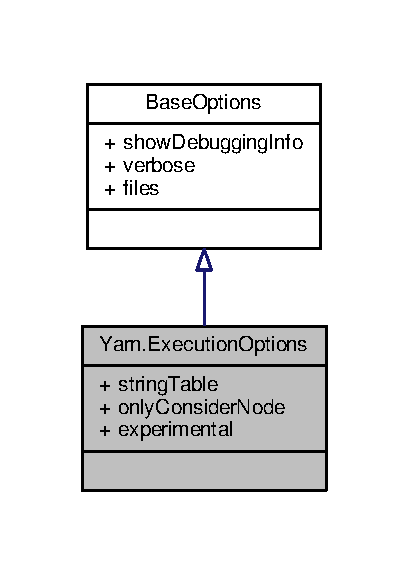
\includegraphics[width=154pt]{a00718}
\end{center}
\end{figure}
\subsection*{Public Member Functions}
\begin{DoxyCompactItemize}
\item 
\hyperlink{a00133_a15924fb79c648f2089ff0db955679dd9}{Line\-Info} (string \hyperlink{a00133_a5a91331fb123e29d71d69e096f943c2f}{node\-Name}, int \hyperlink{a00133_a7165cafce64a3deafc41b2090ddf8d0e}{line\-Number})
\end{DoxyCompactItemize}
\subsection*{Public Attributes}
\begin{DoxyCompactItemize}
\item 
int \hyperlink{a00133_a7165cafce64a3deafc41b2090ddf8d0e}{line\-Number}
\item 
string \hyperlink{a00133_a5a91331fb123e29d71d69e096f943c2f}{node\-Name}
\end{DoxyCompactItemize}


\subsection{Detailed Description}


Definition at line 71 of file Program.\-cs.



\subsection{Constructor \& Destructor Documentation}
\hypertarget{a00133_a15924fb79c648f2089ff0db955679dd9}{\index{Yarn\-::\-Line\-Info@{Yarn\-::\-Line\-Info}!Line\-Info@{Line\-Info}}
\index{Line\-Info@{Line\-Info}!Yarn::LineInfo@{Yarn\-::\-Line\-Info}}
\subsubsection[{Line\-Info}]{\setlength{\rightskip}{0pt plus 5cm}Yarn.\-Line\-Info.\-Line\-Info (
\begin{DoxyParamCaption}
\item[{string}]{node\-Name, }
\item[{int}]{line\-Number}
\end{DoxyParamCaption}
)}}\label{a00133_a15924fb79c648f2089ff0db955679dd9}


Definition at line 76 of file Program.\-cs.



References Yarn.\-Line\-Info.\-line\-Number, and Yarn.\-Line\-Info.\-node\-Name.


\begin{DoxyCode}
77         \{
78             this.nodeName = \hyperlink{a00133_a5a91331fb123e29d71d69e096f943c2f}{nodeName};
79             this.lineNumber = \hyperlink{a00133_a7165cafce64a3deafc41b2090ddf8d0e}{lineNumber};
80         \}
\end{DoxyCode}


\subsection{Member Data Documentation}
\hypertarget{a00133_a7165cafce64a3deafc41b2090ddf8d0e}{\index{Yarn\-::\-Line\-Info@{Yarn\-::\-Line\-Info}!line\-Number@{line\-Number}}
\index{line\-Number@{line\-Number}!Yarn::LineInfo@{Yarn\-::\-Line\-Info}}
\subsubsection[{line\-Number}]{\setlength{\rightskip}{0pt plus 5cm}int Yarn.\-Line\-Info.\-line\-Number}}\label{a00133_a7165cafce64a3deafc41b2090ddf8d0e}


Definition at line 73 of file Program.\-cs.



Referenced by Yarn.\-Line\-Info.\-Line\-Info().

\hypertarget{a00133_a5a91331fb123e29d71d69e096f943c2f}{\index{Yarn\-::\-Line\-Info@{Yarn\-::\-Line\-Info}!node\-Name@{node\-Name}}
\index{node\-Name@{node\-Name}!Yarn::LineInfo@{Yarn\-::\-Line\-Info}}
\subsubsection[{node\-Name}]{\setlength{\rightskip}{0pt plus 5cm}string Yarn.\-Line\-Info.\-node\-Name}}\label{a00133_a5a91331fb123e29d71d69e096f943c2f}


Definition at line 74 of file Program.\-cs.



Referenced by Yarn.\-Line\-Info.\-Line\-Info().



The documentation for this struct was generated from the following file\-:\begin{DoxyCompactItemize}
\item 
Yarn\-Spinner/\hyperlink{a00317}{Program.\-cs}\end{DoxyCompactItemize}

\hypertarget{a00137}{\section{Yarn.\-Loader.\-Node\-Info.\-Position Struct Reference}
\label{a00137}\index{Yarn.\-Loader.\-Node\-Info.\-Position@{Yarn.\-Loader.\-Node\-Info.\-Position}}
}


Collaboration diagram for Yarn.\-Loader.\-Node\-Info.\-Position\-:
\nopagebreak
\begin{figure}[H]
\begin{center}
\leavevmode
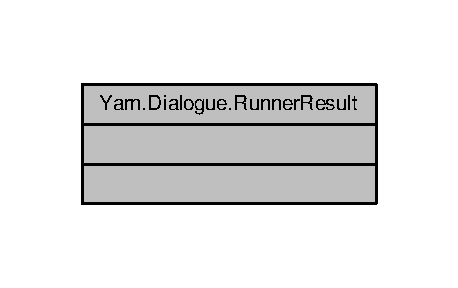
\includegraphics[width=228pt]{a00620}
\end{center}
\end{figure}
\subsection*{Properties}
\begin{DoxyCompactItemize}
\item 
int \hyperlink{a00137_a6b40110781090293fbcd2d6f7695ae4d}{x}\hspace{0.3cm}{\ttfamily  \mbox{[}get, set\mbox{]}}
\item 
int \hyperlink{a00137_a390d560bd9faa3a32d8a0489c69be9e0}{y}\hspace{0.3cm}{\ttfamily  \mbox{[}get, set\mbox{]}}
\end{DoxyCompactItemize}


\subsection{Detailed Description}


Definition at line 246 of file Loader.\-cs.



\subsection{Property Documentation}
\hypertarget{a00137_a6b40110781090293fbcd2d6f7695ae4d}{\index{Yarn\-::\-Loader\-::\-Node\-Info\-::\-Position@{Yarn\-::\-Loader\-::\-Node\-Info\-::\-Position}!x@{x}}
\index{x@{x}!Yarn::Loader::NodeInfo::Position@{Yarn\-::\-Loader\-::\-Node\-Info\-::\-Position}}
\subsubsection[{x}]{\setlength{\rightskip}{0pt plus 5cm}int Yarn.\-Loader.\-Node\-Info.\-Position.\-x\hspace{0.3cm}{\ttfamily [get]}, {\ttfamily [set]}}}\label{a00137_a6b40110781090293fbcd2d6f7695ae4d}


Definition at line 247 of file Loader.\-cs.

\hypertarget{a00137_a390d560bd9faa3a32d8a0489c69be9e0}{\index{Yarn\-::\-Loader\-::\-Node\-Info\-::\-Position@{Yarn\-::\-Loader\-::\-Node\-Info\-::\-Position}!y@{y}}
\index{y@{y}!Yarn::Loader::NodeInfo::Position@{Yarn\-::\-Loader\-::\-Node\-Info\-::\-Position}}
\subsubsection[{y}]{\setlength{\rightskip}{0pt plus 5cm}int Yarn.\-Loader.\-Node\-Info.\-Position.\-y\hspace{0.3cm}{\ttfamily [get]}, {\ttfamily [set]}}}\label{a00137_a390d560bd9faa3a32d8a0489c69be9e0}


Definition at line 248 of file Loader.\-cs.



The documentation for this struct was generated from the following file\-:\begin{DoxyCompactItemize}
\item 
Yarn\-Spinner/\hyperlink{a00288}{Loader.\-cs}\end{DoxyCompactItemize}

\hypertarget{a00138}{\section{Yarn.\-Memory\-Variable\-Store Class Reference}
\label{a00138}\index{Yarn.\-Memory\-Variable\-Store@{Yarn.\-Memory\-Variable\-Store}}
}


Very simple continuity class that keeps all variables in memory.  




Inheritance diagram for Yarn.\-Memory\-Variable\-Store\-:
\nopagebreak
\begin{figure}[H]
\begin{center}
\leavevmode
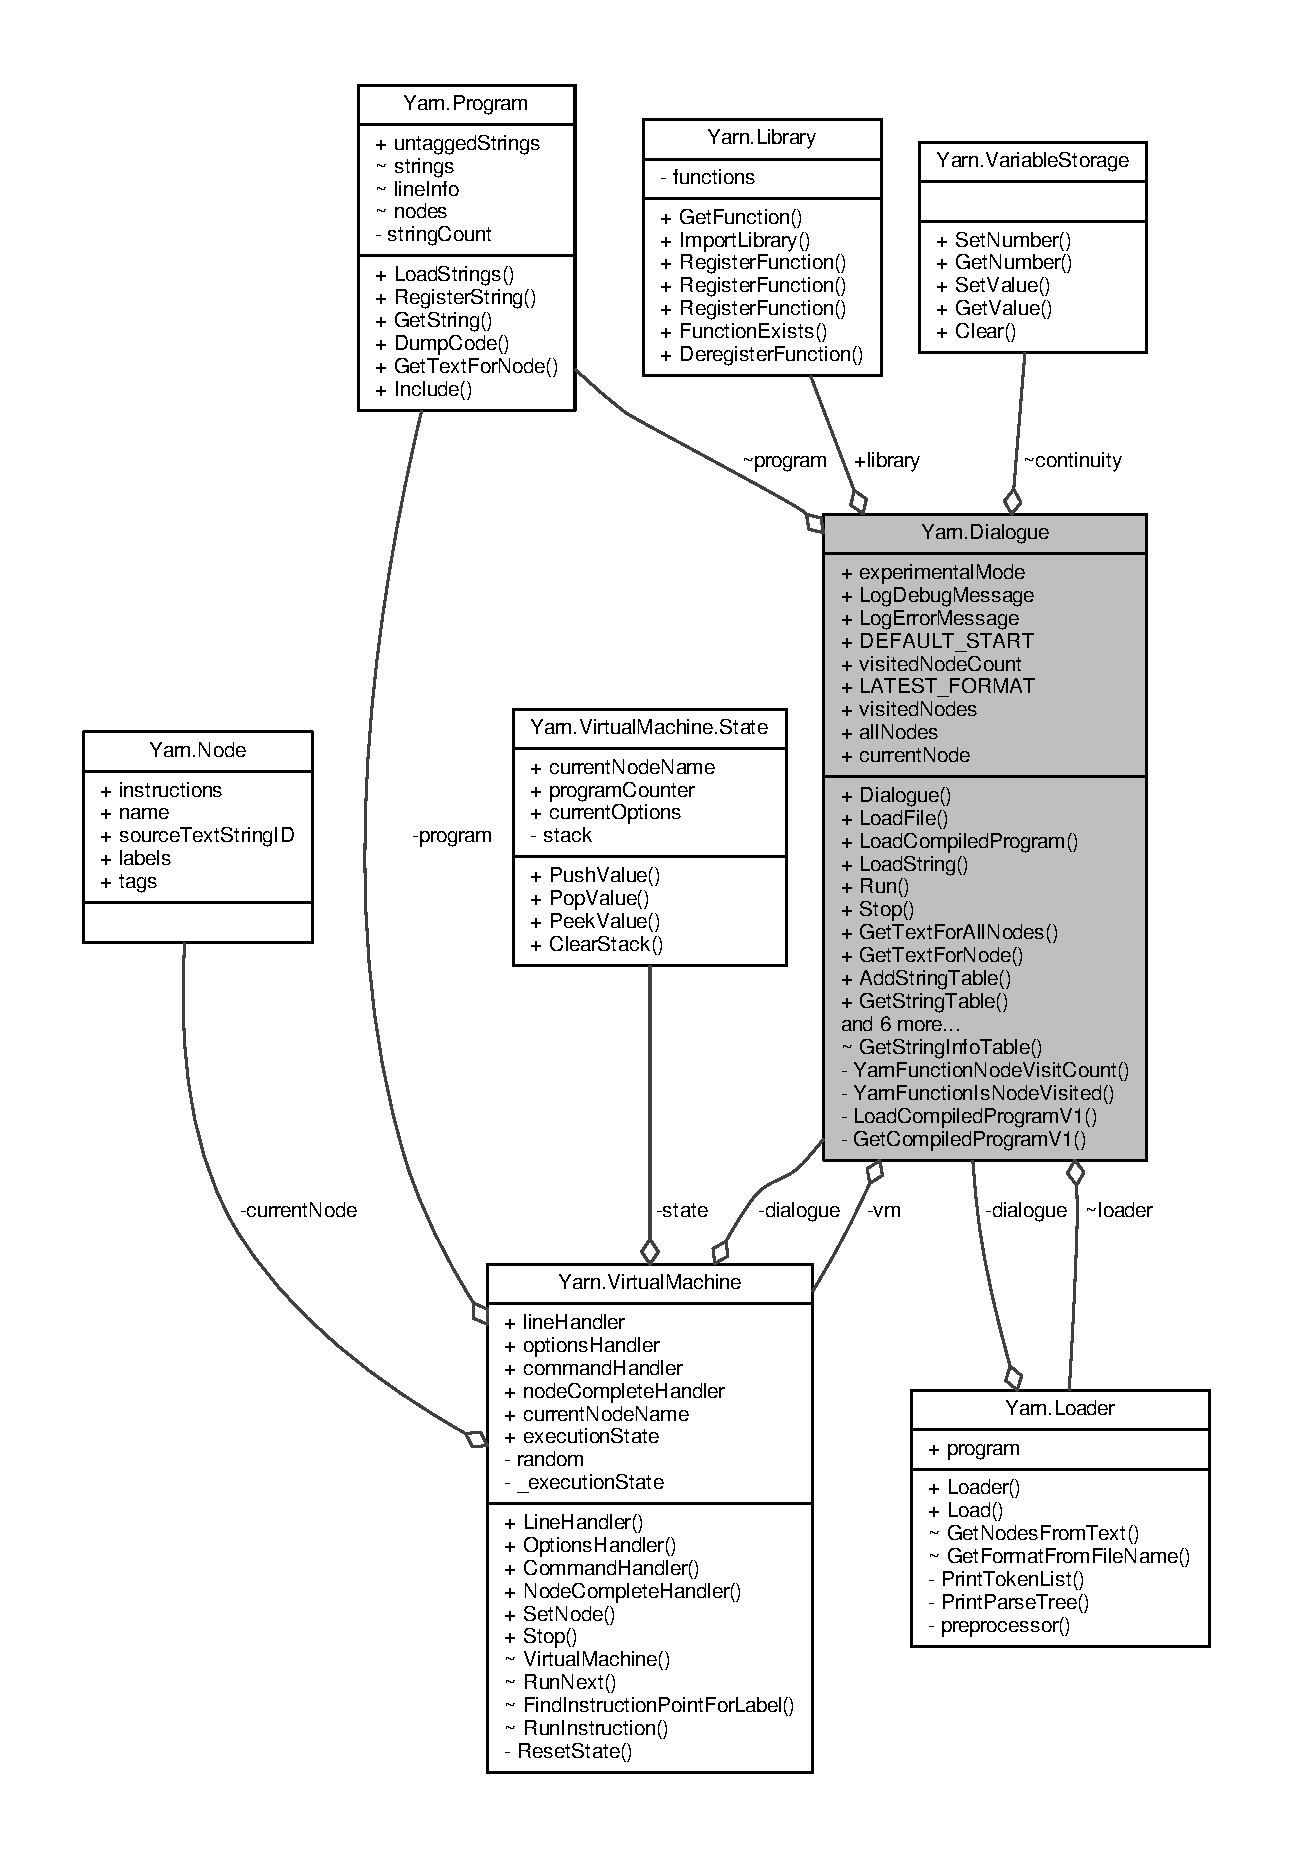
\includegraphics[width=214pt]{a00618}
\end{center}
\end{figure}


Collaboration diagram for Yarn.\-Memory\-Variable\-Store\-:
\nopagebreak
\begin{figure}[H]
\begin{center}
\leavevmode
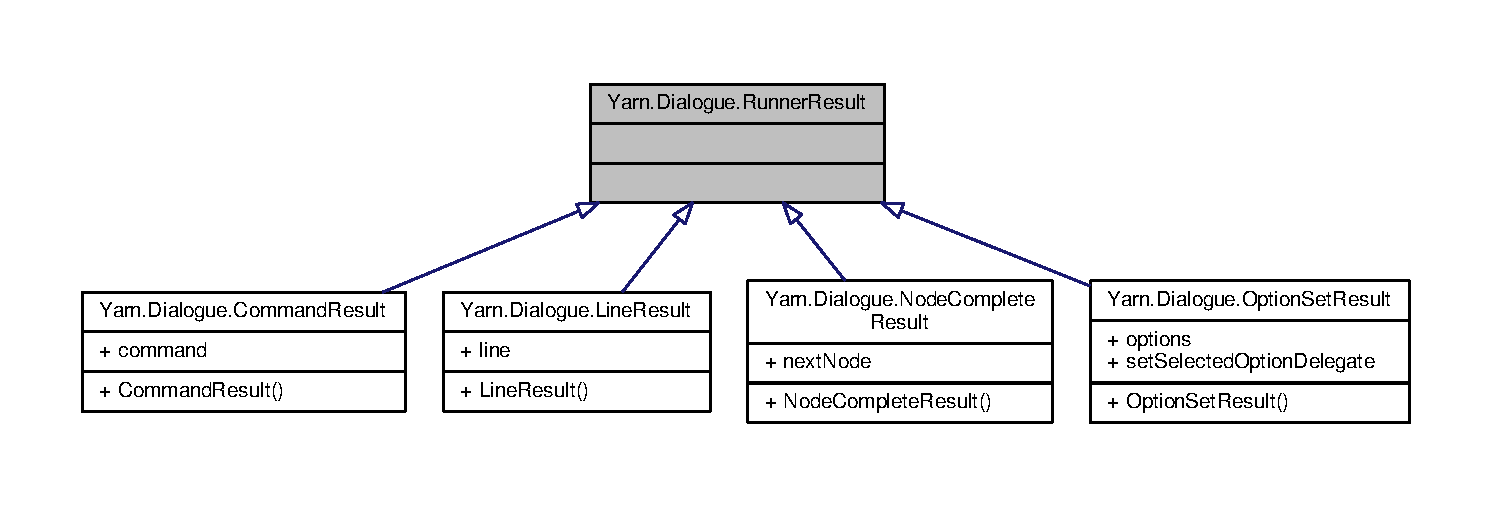
\includegraphics[width=214pt]{a00619}
\end{center}
\end{figure}
\subsection*{Public Member Functions}
\begin{DoxyCompactItemize}
\item 
override void \hyperlink{a00138_a653a459811e5c19549f4b31269093ef5}{Set\-Value} (string variable\-Name, \hyperlink{a00189}{Value} value)
\item 
override \hyperlink{a00189}{Value} \hyperlink{a00138_a0ce77e8245c504a777540e359704aa2a}{Get\-Value} (string variable\-Name)
\item 
override void \hyperlink{a00138_aa6d243e7ef02b91f793a221f509dae69}{Clear} ()
\item 
void \hyperlink{a00044_a48b93de9cd7ae61d0cd9583c8330d3ee}{Set\-Number} (string variable\-Name, float number)
\item 
float \hyperlink{a00044_a1b7f7f4468b2463e7b47986d99362279}{Get\-Number} (string variable\-Name)
\end{DoxyCompactItemize}
\subsection*{Private Attributes}
\begin{DoxyCompactItemize}
\item 
Dictionary$<$ string, \hyperlink{a00189}{Value} $>$ \hyperlink{a00138_aad18acd95297edb8ed496857337f8071}{variables} = new Dictionary$<$string, \hyperlink{a00189}{Value}$>$()
\end{DoxyCompactItemize}


\subsection{Detailed Description}
Very simple continuity class that keeps all variables in memory. 

Definition at line 102 of file Dialogue.\-cs.



\subsection{Member Function Documentation}
\hypertarget{a00138_aa6d243e7ef02b91f793a221f509dae69}{\index{Yarn\-::\-Memory\-Variable\-Store@{Yarn\-::\-Memory\-Variable\-Store}!Clear@{Clear}}
\index{Clear@{Clear}!Yarn::MemoryVariableStore@{Yarn\-::\-Memory\-Variable\-Store}}
\subsubsection[{Clear}]{\setlength{\rightskip}{0pt plus 5cm}override void Yarn.\-Memory\-Variable\-Store.\-Clear (
\begin{DoxyParamCaption}
{}
\end{DoxyParamCaption}
)\hspace{0.3cm}{\ttfamily [virtual]}}}\label{a00138_aa6d243e7ef02b91f793a221f509dae69}


Implements \hyperlink{a00044_a7e45c37f3662ce9f2643e306bb2b3adc}{Yarn.\-Base\-Variable\-Storage}.



Definition at line 123 of file Dialogue.\-cs.


\begin{DoxyCode}
124         \{
125             variables.Clear();
126         \}
\end{DoxyCode}
\hypertarget{a00044_a1b7f7f4468b2463e7b47986d99362279}{\index{Yarn\-::\-Memory\-Variable\-Store@{Yarn\-::\-Memory\-Variable\-Store}!Get\-Number@{Get\-Number}}
\index{Get\-Number@{Get\-Number}!Yarn::MemoryVariableStore@{Yarn\-::\-Memory\-Variable\-Store}}
\subsubsection[{Get\-Number}]{\setlength{\rightskip}{0pt plus 5cm}float Yarn.\-Base\-Variable\-Storage.\-Get\-Number (
\begin{DoxyParamCaption}
\item[{string}]{variable\-Name}
\end{DoxyParamCaption}
)\hspace{0.3cm}{\ttfamily [inherited]}}}\label{a00044_a1b7f7f4468b2463e7b47986d99362279}


Implements \hyperlink{a00192_a04b061c52d8ac814ce559da5286fbc71}{Yarn.\-Variable\-Storage}.



Definition at line 81 of file Dialogue.\-cs.


\begin{DoxyCode}
81                                                     \{
82             \textcolor{keywordflow}{return} this.GetValue(variableName).AsNumber;
83         \}
\end{DoxyCode}
\hypertarget{a00138_a0ce77e8245c504a777540e359704aa2a}{\index{Yarn\-::\-Memory\-Variable\-Store@{Yarn\-::\-Memory\-Variable\-Store}!Get\-Value@{Get\-Value}}
\index{Get\-Value@{Get\-Value}!Yarn::MemoryVariableStore@{Yarn\-::\-Memory\-Variable\-Store}}
\subsubsection[{Get\-Value}]{\setlength{\rightskip}{0pt plus 5cm}override {\bf Value} Yarn.\-Memory\-Variable\-Store.\-Get\-Value (
\begin{DoxyParamCaption}
\item[{string}]{variable\-Name}
\end{DoxyParamCaption}
)\hspace{0.3cm}{\ttfamily [virtual]}}}\label{a00138_a0ce77e8245c504a777540e359704aa2a}


Implements \hyperlink{a00044_a13b142df804d9842e97e628e252928e8}{Yarn.\-Base\-Variable\-Storage}.



Definition at line 111 of file Dialogue.\-cs.



References Yarn.\-Value.\-N\-U\-L\-L, and Yarn.\-Memory\-Variable\-Store.\-variables.


\begin{DoxyCode}
112         \{
113             Value value = \hyperlink{a00189_a1ed2964965baca8621c45efa23f37660}{Value.NULL};
114             \textcolor{keywordflow}{if} (\hyperlink{a00138_aad18acd95297edb8ed496857337f8071}{variables}.ContainsKey(variableName))
115             \{
116 
117                 value = \hyperlink{a00138_aad18acd95297edb8ed496857337f8071}{variables}[variableName];
118 
119             \}
120             \textcolor{keywordflow}{return} value;
121         \}
\end{DoxyCode}
\hypertarget{a00044_a48b93de9cd7ae61d0cd9583c8330d3ee}{\index{Yarn\-::\-Memory\-Variable\-Store@{Yarn\-::\-Memory\-Variable\-Store}!Set\-Number@{Set\-Number}}
\index{Set\-Number@{Set\-Number}!Yarn::MemoryVariableStore@{Yarn\-::\-Memory\-Variable\-Store}}
\subsubsection[{Set\-Number}]{\setlength{\rightskip}{0pt plus 5cm}void Yarn.\-Base\-Variable\-Storage.\-Set\-Number (
\begin{DoxyParamCaption}
\item[{string}]{variable\-Name, }
\item[{float}]{number}
\end{DoxyParamCaption}
)\hspace{0.3cm}{\ttfamily [inherited]}}}\label{a00044_a48b93de9cd7ae61d0cd9583c8330d3ee}


Implements \hyperlink{a00192_aa28c3694f985cf73489efc301b9d41dd}{Yarn.\-Variable\-Storage}.



Definition at line 76 of file Dialogue.\-cs.


\begin{DoxyCode}
76                                                                  \{
77             this.SetValue(variableName, \textcolor{keyword}{new} Value(number));
78         \}
\end{DoxyCode}
\hypertarget{a00138_a653a459811e5c19549f4b31269093ef5}{\index{Yarn\-::\-Memory\-Variable\-Store@{Yarn\-::\-Memory\-Variable\-Store}!Set\-Value@{Set\-Value}}
\index{Set\-Value@{Set\-Value}!Yarn::MemoryVariableStore@{Yarn\-::\-Memory\-Variable\-Store}}
\subsubsection[{Set\-Value}]{\setlength{\rightskip}{0pt plus 5cm}override void Yarn.\-Memory\-Variable\-Store.\-Set\-Value (
\begin{DoxyParamCaption}
\item[{string}]{variable\-Name, }
\item[{{\bf Value}}]{value}
\end{DoxyParamCaption}
)\hspace{0.3cm}{\ttfamily [virtual]}}}\label{a00138_a653a459811e5c19549f4b31269093ef5}


Implements \hyperlink{a00044_a1c57d6d208b78abec0a670396771448e}{Yarn.\-Base\-Variable\-Storage}.



Definition at line 106 of file Dialogue.\-cs.



References Yarn.\-Memory\-Variable\-Store.\-variables.


\begin{DoxyCode}
107         \{
108             \hyperlink{a00138_aad18acd95297edb8ed496857337f8071}{variables}[variableName] = value;
109         \}
\end{DoxyCode}


\subsection{Member Data Documentation}
\hypertarget{a00138_aad18acd95297edb8ed496857337f8071}{\index{Yarn\-::\-Memory\-Variable\-Store@{Yarn\-::\-Memory\-Variable\-Store}!variables@{variables}}
\index{variables@{variables}!Yarn::MemoryVariableStore@{Yarn\-::\-Memory\-Variable\-Store}}
\subsubsection[{variables}]{\setlength{\rightskip}{0pt plus 5cm}Dictionary$<$string, {\bf Value}$>$ Yarn.\-Memory\-Variable\-Store.\-variables = new Dictionary$<$string, {\bf Value}$>$()\hspace{0.3cm}{\ttfamily [private]}}}\label{a00138_aad18acd95297edb8ed496857337f8071}


Definition at line 104 of file Dialogue.\-cs.



Referenced by Yarn.\-Memory\-Variable\-Store.\-Get\-Value(), and Yarn.\-Memory\-Variable\-Store.\-Set\-Value().



The documentation for this class was generated from the following file\-:\begin{DoxyCompactItemize}
\item 
Yarn\-Spinner/\hyperlink{a00308}{Dialogue.\-cs}\end{DoxyCompactItemize}

\hypertarget{a00026}{\section{Csv\-Helper.\-Type\-Conversion.\-Byte\-Converter Class Reference}
\label{a00026}\index{Csv\-Helper.\-Type\-Conversion.\-Byte\-Converter@{Csv\-Helper.\-Type\-Conversion.\-Byte\-Converter}}
}


Converts a Byte to and from a string.  




Inheritance diagram for Csv\-Helper.\-Type\-Conversion.\-Byte\-Converter\-:
\nopagebreak
\begin{figure}[H]
\begin{center}
\leavevmode
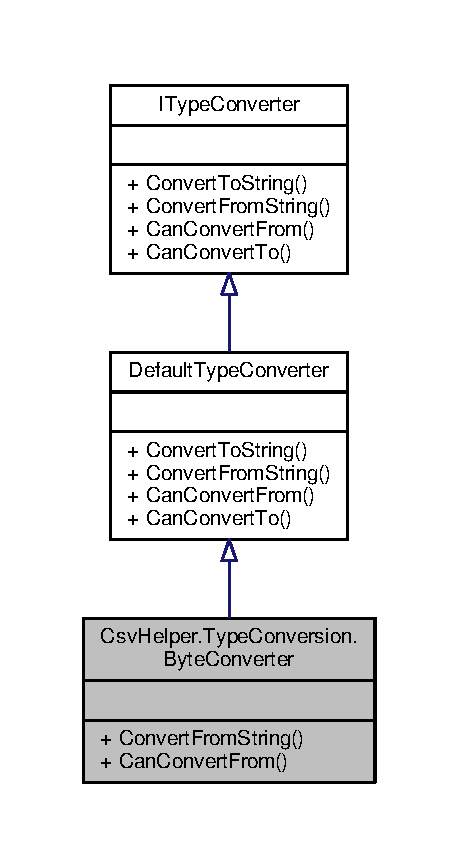
\includegraphics[width=220pt]{de/df8/a00440}
\end{center}
\end{figure}


Collaboration diagram for Csv\-Helper.\-Type\-Conversion.\-Byte\-Converter\-:
\nopagebreak
\begin{figure}[H]
\begin{center}
\leavevmode
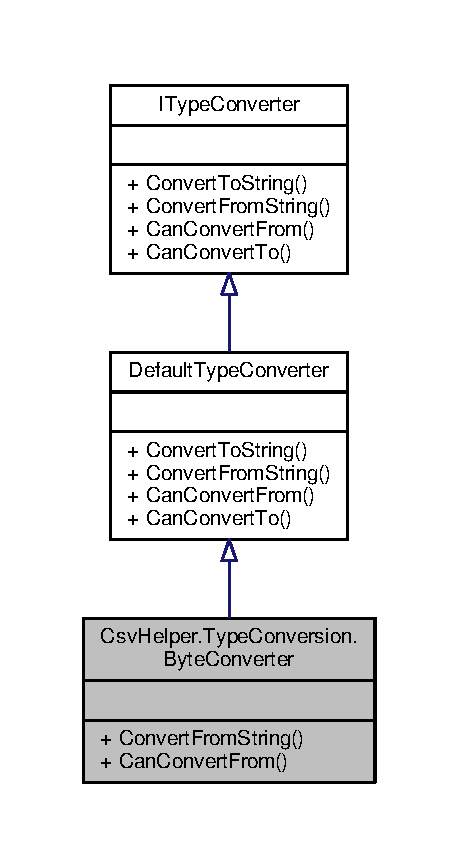
\includegraphics[width=220pt]{d6/d66/a00441}
\end{center}
\end{figure}
\subsection*{Public Member Functions}
\begin{DoxyCompactItemize}
\item 
override object \hyperlink{a00026_a6176d20d761abfc0af4e840553ffae47}{Convert\-From\-String} (\hyperlink{a00154}{Type\-Converter\-Options} options, string text)
\begin{DoxyCompactList}\small\item\em Converts the string to an object. \end{DoxyCompactList}\item 
override bool \hyperlink{a00026_a74a66b405f6c18e69b9fd23a1dea91b0}{Can\-Convert\-From} (Type type)
\begin{DoxyCompactList}\small\item\em Determines whether this instance \mbox{[}can convert from\mbox{]} the specified type. \end{DoxyCompactList}\item 
virtual string \hyperlink{a00068_a36cb2f9b24f15a671293f3a722324c27}{Convert\-To\-String} (\hyperlink{a00154}{Type\-Converter\-Options} options, object value)
\begin{DoxyCompactList}\small\item\em Converts the object to a string. \end{DoxyCompactList}\item 
virtual bool \hyperlink{a00068_acb65bd8c8199d88d5b1629ae35d18514}{Can\-Convert\-To} (Type type)
\begin{DoxyCompactList}\small\item\em Determines whether this instance \mbox{[}can convert to\mbox{]} the specified type. \end{DoxyCompactList}\end{DoxyCompactItemize}


\subsection{Detailed Description}
Converts a Byte to and from a string. 



\subsection{Member Function Documentation}
\hypertarget{a00026_a74a66b405f6c18e69b9fd23a1dea91b0}{\index{Csv\-Helper\-::\-Type\-Conversion\-::\-Byte\-Converter@{Csv\-Helper\-::\-Type\-Conversion\-::\-Byte\-Converter}!Can\-Convert\-From@{Can\-Convert\-From}}
\index{Can\-Convert\-From@{Can\-Convert\-From}!CsvHelper::TypeConversion::ByteConverter@{Csv\-Helper\-::\-Type\-Conversion\-::\-Byte\-Converter}}
\subsubsection[{Can\-Convert\-From}]{\setlength{\rightskip}{0pt plus 5cm}override bool Csv\-Helper.\-Type\-Conversion.\-Byte\-Converter.\-Can\-Convert\-From (
\begin{DoxyParamCaption}
\item[{Type}]{type}
\end{DoxyParamCaption}
)\hspace{0.3cm}{\ttfamily [virtual]}}}\label{a00026_a74a66b405f6c18e69b9fd23a1dea91b0}


Determines whether this instance \mbox{[}can convert from\mbox{]} the specified type. 


\begin{DoxyParams}{Parameters}
{\em type} & The type.\\
\hline
\end{DoxyParams}
\begin{DoxyReturn}{Returns}
{\ttfamily true} if this instance \mbox{[}can convert from\mbox{]} the specified type; otherwise, {\ttfamily false}. 
\end{DoxyReturn}


Reimplemented from \hyperlink{a00068_a470d21adaa704eb281250dbd112ff91a}{Csv\-Helper.\-Type\-Conversion.\-Default\-Type\-Converter}.


\begin{DoxyCode}
42         \{
43             \textcolor{comment}{// We only care about strings.}
44             \textcolor{keywordflow}{return} type == typeof( \textcolor{keywordtype}{string} );
45         \}
\end{DoxyCode}
\hypertarget{a00068_acb65bd8c8199d88d5b1629ae35d18514}{\index{Csv\-Helper\-::\-Type\-Conversion\-::\-Byte\-Converter@{Csv\-Helper\-::\-Type\-Conversion\-::\-Byte\-Converter}!Can\-Convert\-To@{Can\-Convert\-To}}
\index{Can\-Convert\-To@{Can\-Convert\-To}!CsvHelper::TypeConversion::ByteConverter@{Csv\-Helper\-::\-Type\-Conversion\-::\-Byte\-Converter}}
\subsubsection[{Can\-Convert\-To}]{\setlength{\rightskip}{0pt plus 5cm}virtual bool Csv\-Helper.\-Type\-Conversion.\-Default\-Type\-Converter.\-Can\-Convert\-To (
\begin{DoxyParamCaption}
\item[{Type}]{type}
\end{DoxyParamCaption}
)\hspace{0.3cm}{\ttfamily [virtual]}, {\ttfamily [inherited]}}}\label{a00068_acb65bd8c8199d88d5b1629ae35d18514}


Determines whether this instance \mbox{[}can convert to\mbox{]} the specified type. 


\begin{DoxyParams}{Parameters}
{\em type} & The type.\\
\hline
\end{DoxyParams}
\begin{DoxyReturn}{Returns}
{\ttfamily true} if this instance \mbox{[}can convert to\mbox{]} the specified type; otherwise, {\ttfamily false}. 
\end{DoxyReturn}


Implements \hyperlink{a00099_a168b03dad37fcb6882101c93deac8111}{Csv\-Helper.\-Type\-Conversion.\-I\-Type\-Converter}.



Reimplemented in \hyperlink{a00078_a44d625b44f770b945a29cd89e399f90f}{Csv\-Helper.\-Type\-Conversion.\-Enumerable\-Converter}.


\begin{DoxyCode}
70         \{
71             \textcolor{comment}{// We only care about strings.}
72             \textcolor{keywordflow}{return} type == typeof( \textcolor{keywordtype}{string} );
73         \}
\end{DoxyCode}
\hypertarget{a00026_a6176d20d761abfc0af4e840553ffae47}{\index{Csv\-Helper\-::\-Type\-Conversion\-::\-Byte\-Converter@{Csv\-Helper\-::\-Type\-Conversion\-::\-Byte\-Converter}!Convert\-From\-String@{Convert\-From\-String}}
\index{Convert\-From\-String@{Convert\-From\-String}!CsvHelper::TypeConversion::ByteConverter@{Csv\-Helper\-::\-Type\-Conversion\-::\-Byte\-Converter}}
\subsubsection[{Convert\-From\-String}]{\setlength{\rightskip}{0pt plus 5cm}override object Csv\-Helper.\-Type\-Conversion.\-Byte\-Converter.\-Convert\-From\-String (
\begin{DoxyParamCaption}
\item[{{\bf Type\-Converter\-Options}}]{options, }
\item[{string}]{text}
\end{DoxyParamCaption}
)\hspace{0.3cm}{\ttfamily [virtual]}}}\label{a00026_a6176d20d761abfc0af4e840553ffae47}


Converts the string to an object. 


\begin{DoxyParams}{Parameters}
{\em options} & The options to use when converting.\\
\hline
{\em text} & The string to convert to an object.\\
\hline
\end{DoxyParams}
\begin{DoxyReturn}{Returns}
The object created from the string.
\end{DoxyReturn}


Reimplemented from \hyperlink{a00068_a804ea00060e1de70e5151f90d3bfce9b}{Csv\-Helper.\-Type\-Conversion.\-Default\-Type\-Converter}.


\begin{DoxyCode}
22         \{
23             var numberStyle = options.NumberStyle ?? NumberStyles.Integer;
24 
25             byte b;
26             \textcolor{keywordflow}{if}( byte.TryParse( text, numberStyle, options.CultureInfo, out b ) )
27             \{
28                 \textcolor{keywordflow}{return} b;
29             \}
30 
31             \textcolor{keywordflow}{return} base.ConvertFromString( options, text );
32         \}
\end{DoxyCode}
\hypertarget{a00068_a36cb2f9b24f15a671293f3a722324c27}{\index{Csv\-Helper\-::\-Type\-Conversion\-::\-Byte\-Converter@{Csv\-Helper\-::\-Type\-Conversion\-::\-Byte\-Converter}!Convert\-To\-String@{Convert\-To\-String}}
\index{Convert\-To\-String@{Convert\-To\-String}!CsvHelper::TypeConversion::ByteConverter@{Csv\-Helper\-::\-Type\-Conversion\-::\-Byte\-Converter}}
\subsubsection[{Convert\-To\-String}]{\setlength{\rightskip}{0pt plus 5cm}virtual string Csv\-Helper.\-Type\-Conversion.\-Default\-Type\-Converter.\-Convert\-To\-String (
\begin{DoxyParamCaption}
\item[{{\bf Type\-Converter\-Options}}]{options, }
\item[{object}]{value}
\end{DoxyParamCaption}
)\hspace{0.3cm}{\ttfamily [virtual]}, {\ttfamily [inherited]}}}\label{a00068_a36cb2f9b24f15a671293f3a722324c27}


Converts the object to a string. 


\begin{DoxyParams}{Parameters}
{\em options} & The options to use when converting.\\
\hline
{\em value} & The object to convert to a string.\\
\hline
\end{DoxyParams}
\begin{DoxyReturn}{Returns}
The string representation of the object.
\end{DoxyReturn}


Implements \hyperlink{a00099_a90c465c63dbcf913f38aa878f35e77c7}{Csv\-Helper.\-Type\-Conversion.\-I\-Type\-Converter}.



Reimplemented in \hyperlink{a00116_a7205cdb61d2d119582958232b3e63109}{Csv\-Helper.\-Type\-Conversion.\-Nullable\-Converter}, and \hyperlink{a00078_a7e07e9532857d748654d37db590a0e11}{Csv\-Helper.\-Type\-Conversion.\-Enumerable\-Converter}.


\begin{DoxyCode}
22         \{
23             \textcolor{keywordflow}{if}( value == null )
24             \{
25                 \textcolor{keywordflow}{return} string.Empty;
26             \}
27 
28             var formattable = value as IFormattable;
29             \textcolor{keywordflow}{if}( formattable != null )
30             \{
31                 \textcolor{keywordflow}{return} formattable.ToString( options.Format, options.CultureInfo );
32             \}
33 
34             \textcolor{keywordflow}{return} value.ToString();
35         \}
\end{DoxyCode}


The documentation for this class was generated from the following file\-:\begin{DoxyCompactItemize}
\item 
packages/\-Csv\-Helper.\-2.\-16.\-0.\-0/src/\-Csv\-Helper/\-Type\-Conversion/\hyperlink{a00225}{Byte\-Converter.\-cs}\end{DoxyCompactItemize}

\hypertarget{a00154}{\section{Yarn.\-Program Class Reference}
\label{a00154}\index{Yarn.\-Program@{Yarn.\-Program}}
}


Collaboration diagram for Yarn.\-Program\-:
\nopagebreak
\begin{figure}[H]
\begin{center}
\leavevmode
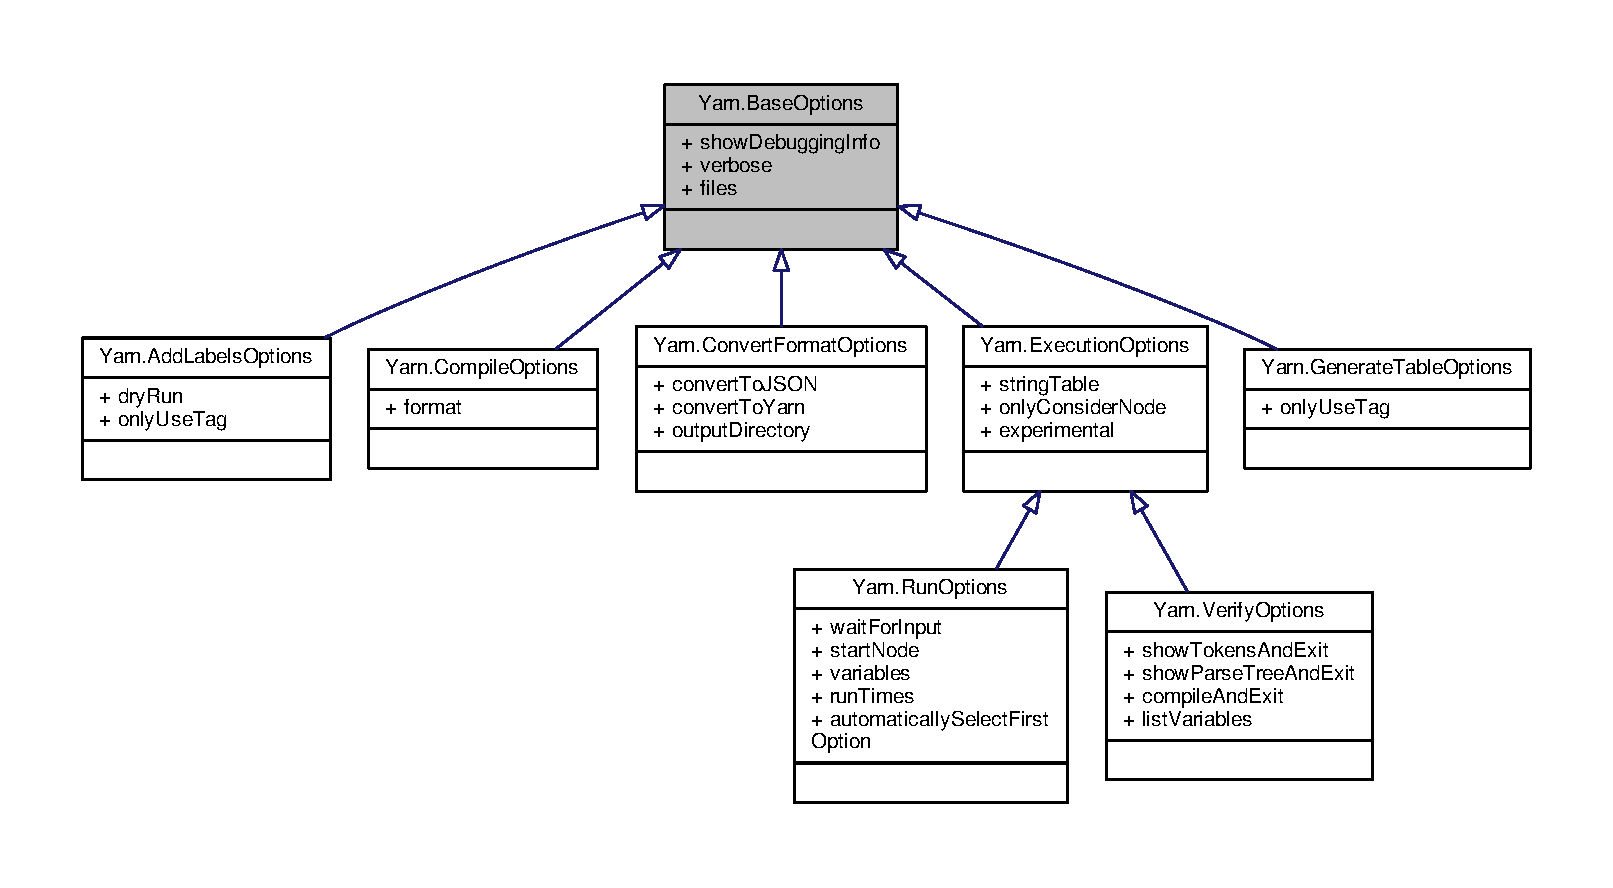
\includegraphics[width=186pt]{a00720}
\end{center}
\end{figure}
\subsection*{Public Member Functions}
\begin{DoxyCompactItemize}
\item 
void \hyperlink{a00154_a977d1ed02e3f6f39d30dfea1663e7927}{Load\-Strings} (Dictionary$<$ string, string $>$ new\-Strings)
\begin{DoxyCompactList}\small\item\em Loads a new string table into the program. \end{DoxyCompactList}\item 
string \hyperlink{a00154_a9baf491479375aa8c3aa2b0c31cf0932}{Register\-String} (string the\-String, string node\-Name, string line\-I\-D, int line\-Number, bool localisable)
\item 
string \hyperlink{a00154_a14737b93594c4aab25c59cb0a3c918f7}{Get\-String} (string key)
\item 
string \hyperlink{a00154_a2f5bb468ce53eb7bbe647e3c11ddbb61}{Dump\-Code} (\hyperlink{a00131}{Library} l)
\item 
string \hyperlink{a00154_aad8029f37832ff1985fad6a31e51afd8}{Get\-Text\-For\-Node} (string node\-Name)
\item 
I\-Enumerable$<$ string $>$ \hyperlink{a00154_a116312a32b20bc18e09f90c9c92a079f}{Get\-Tags\-For\-Node} (string node\-Name)
\item 
void \hyperlink{a00154_afd3385ca1f7589b3b9dae3646e4fee84}{Include} (\hyperlink{a00154}{Program} other\-Program)
\end{DoxyCompactItemize}
\subsection*{Package Attributes}
\begin{DoxyCompactItemize}
\item 
Dictionary$<$ string, string $>$ \hyperlink{a00154_a59263e00cecfe36d9881b4c30b048f09}{strings} = new Dictionary$<$string, string$>$()
\item 
Dictionary$<$ string, \hyperlink{a00133}{Line\-Info} $>$ \hyperlink{a00154_a0d4da395947767b4a1eaaff8a9842adc}{line\-Info} = new Dictionary$<$string, \hyperlink{a00133}{Line\-Info}$>$()
\item 
Dictionary$<$ string, \hyperlink{a00053_a00382}{Node} $>$ \hyperlink{a00154_a3f4928a577c88263ad016be259b175c4}{nodes} = new Dictionary$<$string, \hyperlink{a00053_a00382}{Node}$>$()
\end{DoxyCompactItemize}
\subsection*{Properties}
\begin{DoxyCompactItemize}
\item 
Dictionary$<$ string, string $>$ \hyperlink{a00154_aa8fedbfceaf931d1da3f600eaab6ae87}{untagged\-Strings}\hspace{0.3cm}{\ttfamily  \mbox{[}get\mbox{]}}
\end{DoxyCompactItemize}
\subsection*{Private Attributes}
\begin{DoxyCompactItemize}
\item 
int \hyperlink{a00154_a8ef1d10094ef00311aade6715ba78ec7}{string\-Count} = 0
\end{DoxyCompactItemize}


\subsection{Detailed Description}


Definition at line 84 of file Program.\-cs.



\subsection{Member Function Documentation}
\hypertarget{a00154_a2f5bb468ce53eb7bbe647e3c11ddbb61}{\index{Yarn\-::\-Program@{Yarn\-::\-Program}!Dump\-Code@{Dump\-Code}}
\index{Dump\-Code@{Dump\-Code}!Yarn::Program@{Yarn\-::\-Program}}
\subsubsection[{Dump\-Code}]{\setlength{\rightskip}{0pt plus 5cm}string Yarn.\-Program.\-Dump\-Code (
\begin{DoxyParamCaption}
\item[{{\bf Library}}]{l}
\end{DoxyParamCaption}
)}}\label{a00154_a2f5bb468ce53eb7bbe647e3c11ddbb61}


Definition at line 162 of file Program.\-cs.



References Yarn.\-Program.\-line\-Info, Yarn.\-Program.\-nodes, and Yarn.\-Program.\-strings.


\begin{DoxyCode}
163         \{
164 
165             var sb = \textcolor{keyword}{new} System.Text.StringBuilder();
166 
167             \textcolor{keywordflow}{foreach} (var entry \textcolor{keywordflow}{in} \hyperlink{a00154_a3f4928a577c88263ad016be259b175c4}{nodes})
168             \{
169                 sb.AppendLine(\textcolor{stringliteral}{"Node "} + entry.Key + \textcolor{stringliteral}{":"});
170 
171                 \textcolor{keywordtype}{int} instructionCount = 0;
172                 \textcolor{keywordflow}{foreach} (var instruction \textcolor{keywordflow}{in} entry.Value.instructions)
173                 \{
174                     \textcolor{keywordtype}{string} instructionText;
175 
176                     \textcolor{keywordflow}{if} (instruction.operation == \hyperlink{a00053_ad5dfb6ee68ca7469623ad3e459f98894}{ByteCode}.Label)
177                     \{
178                         instructionText = instruction.ToString(\textcolor{keyword}{this}, l);
179                     \}
180                     \textcolor{keywordflow}{else}
181                     \{
182                         instructionText = \textcolor{stringliteral}{"    "} + instruction.ToString(\textcolor{keyword}{this}, l);
183                     \}
184 
185                     \textcolor{keywordtype}{string} preface;
186 
187                     \textcolor{keywordflow}{if} (instructionCount % 5 == 0 || instructionCount == entry.Value.instructions.Count - 1
      )
188                     \{
189                         preface = string.Format(CultureInfo.InvariantCulture, \textcolor{stringliteral}{"\{0,6\}   "}, instructionCount)
      ;
190                     \}
191                     \textcolor{keywordflow}{else}
192                     \{
193                         preface = string.Format(CultureInfo.InvariantCulture, \textcolor{stringliteral}{"\{0,6\}   "}, \textcolor{stringliteral}{" "});
194                     \}
195 
196                     sb.AppendLine(preface + instructionText);
197 
198                     instructionCount++;
199                 \}
200 
201                 sb.AppendLine();
202             \}
203 
204             sb.AppendLine(\textcolor{stringliteral}{"String table:"});
205 
206             \textcolor{keywordflow}{foreach} (var entry \textcolor{keywordflow}{in} \hyperlink{a00154_a59263e00cecfe36d9881b4c30b048f09}{strings})
207             \{
208                 var \hyperlink{a00154_a0d4da395947767b4a1eaaff8a9842adc}{lineInfo} = this.lineInfo[entry.Key];
209 
210                 sb.AppendLine(string.Format(CultureInfo.InvariantCulture, \textcolor{stringliteral}{"\{0\}: \{1\} (\{2\}:\{3\})"}, entry.Key, 
      entry.Value, lineInfo.nodeName, lineInfo.lineNumber));
211             \}
212 
213             \textcolor{keywordflow}{return} sb.ToString();
214         \}
\end{DoxyCode}
\hypertarget{a00154_a14737b93594c4aab25c59cb0a3c918f7}{\index{Yarn\-::\-Program@{Yarn\-::\-Program}!Get\-String@{Get\-String}}
\index{Get\-String@{Get\-String}!Yarn::Program@{Yarn\-::\-Program}}
\subsubsection[{Get\-String}]{\setlength{\rightskip}{0pt plus 5cm}string Yarn.\-Program.\-Get\-String (
\begin{DoxyParamCaption}
\item[{string}]{key}
\end{DoxyParamCaption}
)}}\label{a00154_a14737b93594c4aab25c59cb0a3c918f7}


Definition at line 155 of file Program.\-cs.


\begin{DoxyCode}
156         \{
157             \textcolor{keywordtype}{string} value = null;
158             strings.TryGetValue(key, out value);
159             \textcolor{keywordflow}{return} value;
160         \}
\end{DoxyCode}
\hypertarget{a00154_a116312a32b20bc18e09f90c9c92a079f}{\index{Yarn\-::\-Program@{Yarn\-::\-Program}!Get\-Tags\-For\-Node@{Get\-Tags\-For\-Node}}
\index{Get\-Tags\-For\-Node@{Get\-Tags\-For\-Node}!Yarn::Program@{Yarn\-::\-Program}}
\subsubsection[{Get\-Tags\-For\-Node}]{\setlength{\rightskip}{0pt plus 5cm}I\-Enumerable$<$string$>$ Yarn.\-Program.\-Get\-Tags\-For\-Node (
\begin{DoxyParamCaption}
\item[{string}]{node\-Name}
\end{DoxyParamCaption}
)}}\label{a00154_a116312a32b20bc18e09f90c9c92a079f}


Definition at line 221 of file Program.\-cs.



References Yarn.\-Program.\-nodes.


\begin{DoxyCode}
222         \{
223             \textcolor{keywordflow}{return} \hyperlink{a00154_a3f4928a577c88263ad016be259b175c4}{nodes}[nodeName].tags;
224         \}
\end{DoxyCode}
\hypertarget{a00154_aad8029f37832ff1985fad6a31e51afd8}{\index{Yarn\-::\-Program@{Yarn\-::\-Program}!Get\-Text\-For\-Node@{Get\-Text\-For\-Node}}
\index{Get\-Text\-For\-Node@{Get\-Text\-For\-Node}!Yarn::Program@{Yarn\-::\-Program}}
\subsubsection[{Get\-Text\-For\-Node}]{\setlength{\rightskip}{0pt plus 5cm}string Yarn.\-Program.\-Get\-Text\-For\-Node (
\begin{DoxyParamCaption}
\item[{string}]{node\-Name}
\end{DoxyParamCaption}
)}}\label{a00154_aad8029f37832ff1985fad6a31e51afd8}


Definition at line 216 of file Program.\-cs.



References Yarn.\-Program.\-nodes.


\begin{DoxyCode}
217         \{
218             \textcolor{keywordflow}{return} this.GetString(\hyperlink{a00154_a3f4928a577c88263ad016be259b175c4}{nodes}[nodeName].sourceTextStringID);
219         \}
\end{DoxyCode}
\hypertarget{a00154_afd3385ca1f7589b3b9dae3646e4fee84}{\index{Yarn\-::\-Program@{Yarn\-::\-Program}!Include@{Include}}
\index{Include@{Include}!Yarn::Program@{Yarn\-::\-Program}}
\subsubsection[{Include}]{\setlength{\rightskip}{0pt plus 5cm}void Yarn.\-Program.\-Include (
\begin{DoxyParamCaption}
\item[{{\bf Program}}]{other\-Program}
\end{DoxyParamCaption}
)}}\label{a00154_afd3385ca1f7589b3b9dae3646e4fee84}


Definition at line 226 of file Program.\-cs.



References Yarn.\-Program.\-nodes, and Yarn.\-Program.\-strings.


\begin{DoxyCode}
227         \{
228             \textcolor{keywordflow}{foreach} (var otherNodeName \textcolor{keywordflow}{in} otherProgram.nodes)
229             \{
230 
231                 \textcolor{keywordflow}{if} (\hyperlink{a00154_a3f4928a577c88263ad016be259b175c4}{nodes}.ContainsKey(otherNodeName.Key))
232                 \{
233                     \textcolor{keywordflow}{throw} \textcolor{keyword}{new} InvalidOperationException(\textcolor{keywordtype}{string}.Format(CultureInfo.CurrentCulture, \textcolor{stringliteral}{"This
       program already contains a node named \{0\}"}, otherNodeName.Key));
234                 \}
235 
236                 \hyperlink{a00154_a3f4928a577c88263ad016be259b175c4}{nodes}[otherNodeName.Key] = otherNodeName.Value;
237             \}
238 
239             \textcolor{keywordflow}{foreach} (var otherString \textcolor{keywordflow}{in} otherProgram.strings)
240             \{
241 
242                 \textcolor{keywordflow}{if} (\hyperlink{a00154_a3f4928a577c88263ad016be259b175c4}{nodes}.ContainsKey(otherString.Key))
243                 \{
244                     \textcolor{keywordflow}{throw} \textcolor{keyword}{new} InvalidOperationException(\textcolor{keywordtype}{string}.Format(CultureInfo.CurrentCulture, \textcolor{stringliteral}{"This
       program already contains a string with key \{0\}"}, otherString.Key));
245                 \}
246 
247                 \hyperlink{a00154_a59263e00cecfe36d9881b4c30b048f09}{strings}[otherString.Key] = otherString.Value;
248             \}
249         \}
\end{DoxyCode}
\hypertarget{a00154_a977d1ed02e3f6f39d30dfea1663e7927}{\index{Yarn\-::\-Program@{Yarn\-::\-Program}!Load\-Strings@{Load\-Strings}}
\index{Load\-Strings@{Load\-Strings}!Yarn::Program@{Yarn\-::\-Program}}
\subsubsection[{Load\-Strings}]{\setlength{\rightskip}{0pt plus 5cm}void Yarn.\-Program.\-Load\-Strings (
\begin{DoxyParamCaption}
\item[{Dictionary$<$ string, string $>$}]{new\-Strings}
\end{DoxyParamCaption}
)}}\label{a00154_a977d1ed02e3f6f39d30dfea1663e7927}


Loads a new string table into the program. 

The string table is merged with any existing strings, with the new table taking precedence over the old. 

Definition at line 125 of file Program.\-cs.



References Yarn.\-Program.\-strings.


\begin{DoxyCode}
126         \{
127             \textcolor{keywordflow}{foreach} (var entry \textcolor{keywordflow}{in} newStrings)
128             \{
129                 \hyperlink{a00154_a59263e00cecfe36d9881b4c30b048f09}{strings}[entry.Key] = entry.Value;
130             \}
131         \}
\end{DoxyCode}
\hypertarget{a00154_a9baf491479375aa8c3aa2b0c31cf0932}{\index{Yarn\-::\-Program@{Yarn\-::\-Program}!Register\-String@{Register\-String}}
\index{Register\-String@{Register\-String}!Yarn::Program@{Yarn\-::\-Program}}
\subsubsection[{Register\-String}]{\setlength{\rightskip}{0pt plus 5cm}string Yarn.\-Program.\-Register\-String (
\begin{DoxyParamCaption}
\item[{string}]{the\-String, }
\item[{string}]{node\-Name, }
\item[{string}]{line\-I\-D, }
\item[{int}]{line\-Number, }
\item[{bool}]{localisable}
\end{DoxyParamCaption}
)}}\label{a00154_a9baf491479375aa8c3aa2b0c31cf0932}


Definition at line 133 of file Program.\-cs.



References Yarn.\-Program.\-string\-Count.


\begin{DoxyCode}
134         \{
135 
136             \textcolor{keywordtype}{string} key;
137 
138             \textcolor{keywordflow}{if} (lineID == null)
139                 key = string.Format(CultureInfo.InvariantCulture, \textcolor{stringliteral}{"\{0\}-\{1\}"}, nodeName, 
      \hyperlink{a00154_a8ef1d10094ef00311aade6715ba78ec7}{stringCount}++);
140             \textcolor{keywordflow}{else}
141                 key = lineID;
142 
143             \textcolor{comment}{// It's not in the list; append it}
144             strings.Add(key, theString);
145 
146             \textcolor{keywordflow}{if} (localisable)
147             \{
148                 \textcolor{comment}{// Additionally, keep info about this string around}
149                 lineInfo.Add(key, \textcolor{keyword}{new} LineInfo(nodeName, lineNumber));
150             \}
151 
152             \textcolor{keywordflow}{return} key;
153         \}
\end{DoxyCode}


\subsection{Member Data Documentation}
\hypertarget{a00154_a0d4da395947767b4a1eaaff8a9842adc}{\index{Yarn\-::\-Program@{Yarn\-::\-Program}!line\-Info@{line\-Info}}
\index{line\-Info@{line\-Info}!Yarn::Program@{Yarn\-::\-Program}}
\subsubsection[{line\-Info}]{\setlength{\rightskip}{0pt plus 5cm}Dictionary$<$string, {\bf Line\-Info}$>$ Yarn.\-Program.\-line\-Info = new Dictionary$<$string, {\bf Line\-Info}$>$()\hspace{0.3cm}{\ttfamily [package]}}}\label{a00154_a0d4da395947767b4a1eaaff8a9842adc}


Definition at line 88 of file Program.\-cs.



Referenced by Yarn.\-Program.\-Dump\-Code().

\hypertarget{a00154_a3f4928a577c88263ad016be259b175c4}{\index{Yarn\-::\-Program@{Yarn\-::\-Program}!nodes@{nodes}}
\index{nodes@{nodes}!Yarn::Program@{Yarn\-::\-Program}}
\subsubsection[{nodes}]{\setlength{\rightskip}{0pt plus 5cm}Dictionary$<$string, {\bf Node}$>$ Yarn.\-Program.\-nodes = new Dictionary$<$string, {\bf Node}$>$()\hspace{0.3cm}{\ttfamily [package]}}}\label{a00154_a3f4928a577c88263ad016be259b175c4}


Definition at line 91 of file Program.\-cs.



Referenced by Yarn.\-Compiler.\-Compile\-Node(), Yarn.\-Program.\-Dump\-Code(), Yarn.\-Dialogue.\-Get\-Tags\-For\-All\-Nodes(), Yarn.\-Program.\-Get\-Tags\-For\-Node(), Yarn.\-Dialogue.\-Get\-Tags\-For\-Node(), Yarn.\-Dialogue.\-Get\-Text\-For\-All\-Nodes(), Yarn.\-Program.\-Get\-Text\-For\-Node(), Yarn.\-Dialogue.\-Get\-Text\-For\-Node(), Yarn.\-Program.\-Include(), Yarn.\-Dialogue.\-Node\-Exists(), and Yarn.\-Virtual\-Machine.\-Set\-Node().

\hypertarget{a00154_a8ef1d10094ef00311aade6715ba78ec7}{\index{Yarn\-::\-Program@{Yarn\-::\-Program}!string\-Count@{string\-Count}}
\index{string\-Count@{string\-Count}!Yarn::Program@{Yarn\-::\-Program}}
\subsubsection[{string\-Count}]{\setlength{\rightskip}{0pt plus 5cm}int Yarn.\-Program.\-string\-Count = 0\hspace{0.3cm}{\ttfamily [private]}}}\label{a00154_a8ef1d10094ef00311aade6715ba78ec7}


Definition at line 119 of file Program.\-cs.



Referenced by Yarn.\-Program.\-Register\-String().

\hypertarget{a00154_a59263e00cecfe36d9881b4c30b048f09}{\index{Yarn\-::\-Program@{Yarn\-::\-Program}!strings@{strings}}
\index{strings@{strings}!Yarn::Program@{Yarn\-::\-Program}}
\subsubsection[{strings}]{\setlength{\rightskip}{0pt plus 5cm}Dictionary$<$string, string$>$ Yarn.\-Program.\-strings = new Dictionary$<$string, string$>$()\hspace{0.3cm}{\ttfamily [package]}}}\label{a00154_a59263e00cecfe36d9881b4c30b048f09}


Definition at line 87 of file Program.\-cs.



Referenced by Yarn.\-Program.\-Dump\-Code(), Yarn.\-Program.\-Include(), and Yarn.\-Program.\-Load\-Strings().



\subsection{Property Documentation}
\hypertarget{a00154_aa8fedbfceaf931d1da3f600eaab6ae87}{\index{Yarn\-::\-Program@{Yarn\-::\-Program}!untagged\-Strings@{untagged\-Strings}}
\index{untagged\-Strings@{untagged\-Strings}!Yarn::Program@{Yarn\-::\-Program}}
\subsubsection[{untagged\-Strings}]{\setlength{\rightskip}{0pt plus 5cm}Dictionary$<$string, string$>$ Yarn.\-Program.\-untagged\-Strings\hspace{0.3cm}{\ttfamily [get]}, {\ttfamily [package]}}}\label{a00154_aa8fedbfceaf931d1da3f600eaab6ae87}


Definition at line 103 of file Program.\-cs.



The documentation for this class was generated from the following file\-:\begin{DoxyCompactItemize}
\item 
Yarn\-Spinner/\hyperlink{a00317}{Program.\-cs}\end{DoxyCompactItemize}

\hypertarget{a00155}{\section{Yarn.\-Virtual\-Machine.\-State Class Reference}
\label{a00155}\index{Yarn.\-Virtual\-Machine.\-State@{Yarn.\-Virtual\-Machine.\-State}}
}


Collaboration diagram for Yarn.\-Virtual\-Machine.\-State\-:
\nopagebreak
\begin{figure}[H]
\begin{center}
\leavevmode
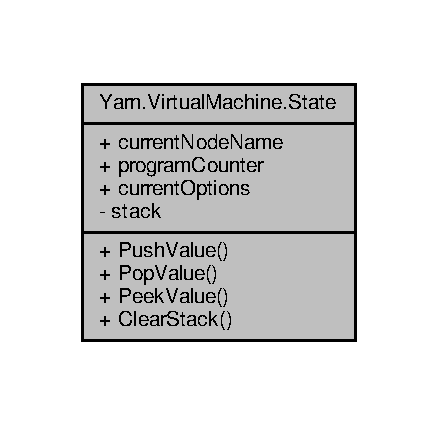
\includegraphics[width=210pt]{a00708}
\end{center}
\end{figure}
\subsection*{Public Member Functions}
\begin{DoxyCompactItemize}
\item 
void \hyperlink{a00155_aace44f5b85b9f746fede834becda4a8e}{Push\-Value} (object o)
\begin{DoxyCompactList}\small\item\em Methods for working with the stack. \end{DoxyCompactList}\item 
\hyperlink{a00177}{Value} \hyperlink{a00155_a36881a888ea2839d74c3d4e7c199f4ee}{Pop\-Value} ()
\begin{DoxyCompactList}\small\item\em Pop a value from the stack. \end{DoxyCompactList}\item 
\hyperlink{a00177}{Value} \hyperlink{a00155_a54fd5b64ec94e937e771846167242dc2}{Peek\-Value} ()
\begin{DoxyCompactList}\small\item\em Peek at a value from the stack. \end{DoxyCompactList}\item 
void \hyperlink{a00155_a9c787097fbbbbf1680e4960cda092535}{Clear\-Stack} ()
\begin{DoxyCompactList}\small\item\em Clear the stack. \end{DoxyCompactList}\end{DoxyCompactItemize}
\subsection*{Public Attributes}
\begin{DoxyCompactItemize}
\item 
string \hyperlink{a00155_a86f481fad527f719b49f8fee6ff79764}{current\-Node\-Name}
\begin{DoxyCompactList}\small\item\em The name of the node that we're currently in. \end{DoxyCompactList}\item 
int \hyperlink{a00155_a2c76546b54b4fb573d7f14d79ce230a3}{program\-Counter} = 0
\begin{DoxyCompactList}\small\item\em The instruction number in the current node. \end{DoxyCompactList}\item 
List$<$ Key\-Value\-Pair$<$ string, \\*
string $>$ $>$ \hyperlink{a00155_ab816dfea32ecda23282700f01454e0a9}{current\-Options} = new List$<$Key\-Value\-Pair$<$string, string$>$$>$()
\begin{DoxyCompactList}\small\item\em List of options, where each option = $<$string id, destination node$>$ \end{DoxyCompactList}\end{DoxyCompactItemize}
\subsection*{Private Attributes}
\begin{DoxyCompactItemize}
\item 
Stack$<$ \hyperlink{a00177}{Value} $>$ \hyperlink{a00155_a0bc84abf38b3ff31cbb47363b851c233}{stack} = new Stack$<$\hyperlink{a00177}{Value}$>$()
\begin{DoxyCompactList}\small\item\em The value stack. \end{DoxyCompactList}\end{DoxyCompactItemize}


\subsection{Detailed Description}


Definition at line 9 of file Virtual\-Machine.\-cs.



\subsection{Member Function Documentation}
\hypertarget{a00155_a9c787097fbbbbf1680e4960cda092535}{\index{Yarn\-::\-Virtual\-Machine\-::\-State@{Yarn\-::\-Virtual\-Machine\-::\-State}!Clear\-Stack@{Clear\-Stack}}
\index{Clear\-Stack@{Clear\-Stack}!Yarn::VirtualMachine::State@{Yarn\-::\-Virtual\-Machine\-::\-State}}
\subsubsection[{Clear\-Stack}]{\setlength{\rightskip}{0pt plus 5cm}void Yarn.\-Virtual\-Machine.\-State.\-Clear\-Stack (
\begin{DoxyParamCaption}
{}
\end{DoxyParamCaption}
)}}\label{a00155_a9c787097fbbbbf1680e4960cda092535}


Clear the stack. 



Definition at line 43 of file Virtual\-Machine.\-cs.


\begin{DoxyCode}
43                                      \{
44                 stack.Clear ();
45             \}
\end{DoxyCode}
\hypertarget{a00155_a54fd5b64ec94e937e771846167242dc2}{\index{Yarn\-::\-Virtual\-Machine\-::\-State@{Yarn\-::\-Virtual\-Machine\-::\-State}!Peek\-Value@{Peek\-Value}}
\index{Peek\-Value@{Peek\-Value}!Yarn::VirtualMachine::State@{Yarn\-::\-Virtual\-Machine\-::\-State}}
\subsubsection[{Peek\-Value}]{\setlength{\rightskip}{0pt plus 5cm}{\bf Value} Yarn.\-Virtual\-Machine.\-State.\-Peek\-Value (
\begin{DoxyParamCaption}
{}
\end{DoxyParamCaption}
)}}\label{a00155_a54fd5b64ec94e937e771846167242dc2}


Peek at a value from the stack. 



Definition at line 38 of file Virtual\-Machine.\-cs.



Referenced by Yarn.\-Virtual\-Machine.\-Run\-Instruction().


\begin{DoxyCode}
38                                      \{
39                 \textcolor{keywordflow}{return} stack.Peek ();
40             \}
\end{DoxyCode}


Here is the caller graph for this function\-:
\nopagebreak
\begin{figure}[H]
\begin{center}
\leavevmode
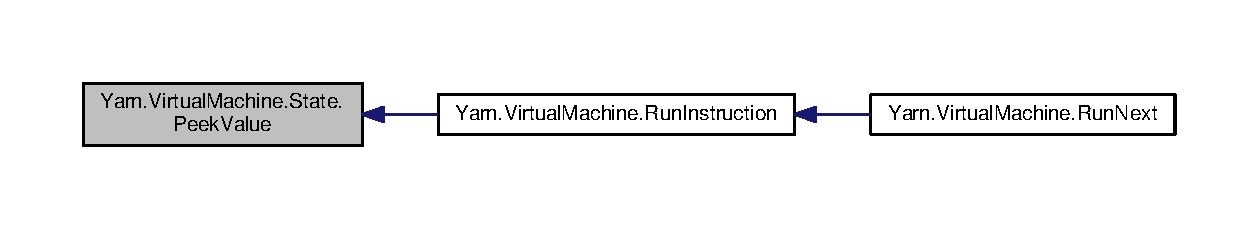
\includegraphics[width=350pt]{a00155_a54fd5b64ec94e937e771846167242dc2_icgraph}
\end{center}
\end{figure}


\hypertarget{a00155_a36881a888ea2839d74c3d4e7c199f4ee}{\index{Yarn\-::\-Virtual\-Machine\-::\-State@{Yarn\-::\-Virtual\-Machine\-::\-State}!Pop\-Value@{Pop\-Value}}
\index{Pop\-Value@{Pop\-Value}!Yarn::VirtualMachine::State@{Yarn\-::\-Virtual\-Machine\-::\-State}}
\subsubsection[{Pop\-Value}]{\setlength{\rightskip}{0pt plus 5cm}{\bf Value} Yarn.\-Virtual\-Machine.\-State.\-Pop\-Value (
\begin{DoxyParamCaption}
{}
\end{DoxyParamCaption}
)}}\label{a00155_a36881a888ea2839d74c3d4e7c199f4ee}


Pop a value from the stack. 



Definition at line 33 of file Virtual\-Machine.\-cs.



Referenced by Yarn.\-Virtual\-Machine.\-Run\-Instruction().


\begin{DoxyCode}
33                                     \{
34                 \textcolor{keywordflow}{return} stack.Pop ();
35             \}
\end{DoxyCode}


Here is the caller graph for this function\-:
\nopagebreak
\begin{figure}[H]
\begin{center}
\leavevmode
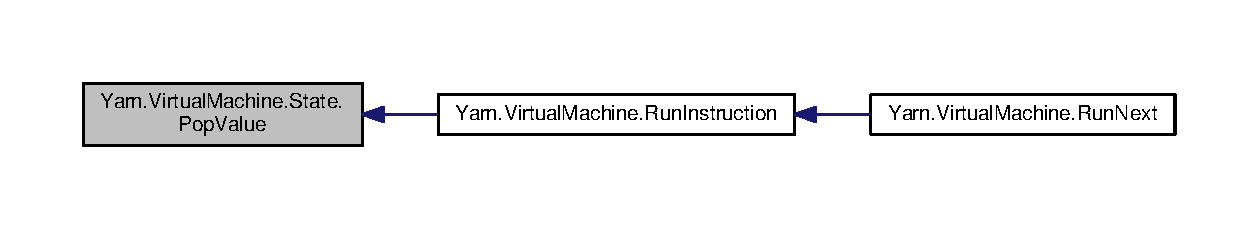
\includegraphics[width=350pt]{a00155_a36881a888ea2839d74c3d4e7c199f4ee_icgraph}
\end{center}
\end{figure}


\hypertarget{a00155_aace44f5b85b9f746fede834becda4a8e}{\index{Yarn\-::\-Virtual\-Machine\-::\-State@{Yarn\-::\-Virtual\-Machine\-::\-State}!Push\-Value@{Push\-Value}}
\index{Push\-Value@{Push\-Value}!Yarn::VirtualMachine::State@{Yarn\-::\-Virtual\-Machine\-::\-State}}
\subsubsection[{Push\-Value}]{\setlength{\rightskip}{0pt plus 5cm}void Yarn.\-Virtual\-Machine.\-State.\-Push\-Value (
\begin{DoxyParamCaption}
\item[{object}]{o}
\end{DoxyParamCaption}
)}}\label{a00155_aace44f5b85b9f746fede834becda4a8e}


Methods for working with the stack. 



Definition at line 24 of file Virtual\-Machine.\-cs.


\begin{DoxyCode}
24                                             \{
25                 \textcolor{keywordflow}{if}( o is Value ) \{
26                     stack.Push(o as Value);
27                 \} \textcolor{keywordflow}{else} \{
28                     stack.Push (\textcolor{keyword}{new} Value(o));
29                 \}
30             \}
\end{DoxyCode}


\subsection{Member Data Documentation}
\hypertarget{a00155_a86f481fad527f719b49f8fee6ff79764}{\index{Yarn\-::\-Virtual\-Machine\-::\-State@{Yarn\-::\-Virtual\-Machine\-::\-State}!current\-Node\-Name@{current\-Node\-Name}}
\index{current\-Node\-Name@{current\-Node\-Name}!Yarn::VirtualMachine::State@{Yarn\-::\-Virtual\-Machine\-::\-State}}
\subsubsection[{current\-Node\-Name}]{\setlength{\rightskip}{0pt plus 5cm}string Yarn.\-Virtual\-Machine.\-State.\-current\-Node\-Name}}\label{a00155_a86f481fad527f719b49f8fee6ff79764}


The name of the node that we're currently in. 



Definition at line 12 of file Virtual\-Machine.\-cs.



Referenced by Yarn.\-Virtual\-Machine.\-Find\-Instruction\-Point\-For\-Label().

\hypertarget{a00155_ab816dfea32ecda23282700f01454e0a9}{\index{Yarn\-::\-Virtual\-Machine\-::\-State@{Yarn\-::\-Virtual\-Machine\-::\-State}!current\-Options@{current\-Options}}
\index{current\-Options@{current\-Options}!Yarn::VirtualMachine::State@{Yarn\-::\-Virtual\-Machine\-::\-State}}
\subsubsection[{current\-Options}]{\setlength{\rightskip}{0pt plus 5cm}List$<$Key\-Value\-Pair$<$string,string$>$ $>$ Yarn.\-Virtual\-Machine.\-State.\-current\-Options = new List$<$Key\-Value\-Pair$<$string, string$>$$>$()}}\label{a00155_ab816dfea32ecda23282700f01454e0a9}


List of options, where each option = $<$string id, destination node$>$ 



Definition at line 18 of file Virtual\-Machine.\-cs.



Referenced by Yarn.\-Virtual\-Machine.\-Run\-Instruction().

\hypertarget{a00155_a2c76546b54b4fb573d7f14d79ce230a3}{\index{Yarn\-::\-Virtual\-Machine\-::\-State@{Yarn\-::\-Virtual\-Machine\-::\-State}!program\-Counter@{program\-Counter}}
\index{program\-Counter@{program\-Counter}!Yarn::VirtualMachine::State@{Yarn\-::\-Virtual\-Machine\-::\-State}}
\subsubsection[{program\-Counter}]{\setlength{\rightskip}{0pt plus 5cm}int Yarn.\-Virtual\-Machine.\-State.\-program\-Counter = 0}}\label{a00155_a2c76546b54b4fb573d7f14d79ce230a3}


The instruction number in the current node. 



Definition at line 15 of file Virtual\-Machine.\-cs.



Referenced by Yarn.\-Virtual\-Machine.\-Run\-Next().

\hypertarget{a00155_a0bc84abf38b3ff31cbb47363b851c233}{\index{Yarn\-::\-Virtual\-Machine\-::\-State@{Yarn\-::\-Virtual\-Machine\-::\-State}!stack@{stack}}
\index{stack@{stack}!Yarn::VirtualMachine::State@{Yarn\-::\-Virtual\-Machine\-::\-State}}
\subsubsection[{stack}]{\setlength{\rightskip}{0pt plus 5cm}Stack$<${\bf Value}$>$ Yarn.\-Virtual\-Machine.\-State.\-stack = new Stack$<${\bf Value}$>$()\hspace{0.3cm}{\ttfamily [private]}}}\label{a00155_a0bc84abf38b3ff31cbb47363b851c233}


The value stack. 



Definition at line 21 of file Virtual\-Machine.\-cs.



The documentation for this class was generated from the following file\-:\begin{DoxyCompactItemize}
\item 
Yarn\-Spinner/\hyperlink{a00298}{Virtual\-Machine.\-cs}\end{DoxyCompactItemize}

\hypertarget{a00156}{\section{Yarn.\-Dialogue.\-Runner\-Result Class Reference}
\label{a00156}\index{Yarn.\-Dialogue.\-Runner\-Result@{Yarn.\-Dialogue.\-Runner\-Result}}
}


Represents something for the end user (\char`\"{}client\char`\"{}) of the \hyperlink{a00092}{Dialogue} class to do.  




Inheritance diagram for Yarn.\-Dialogue.\-Runner\-Result\-:
\nopagebreak
\begin{figure}[H]
\begin{center}
\leavevmode
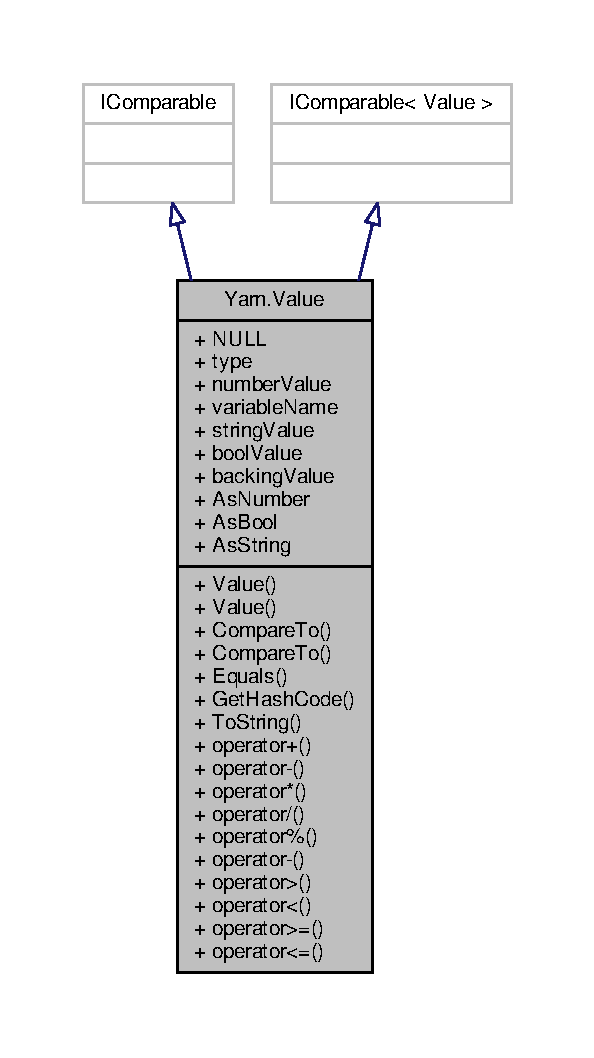
\includegraphics[width=350pt]{a00631}
\end{center}
\end{figure}


Collaboration diagram for Yarn.\-Dialogue.\-Runner\-Result\-:
\nopagebreak
\begin{figure}[H]
\begin{center}
\leavevmode
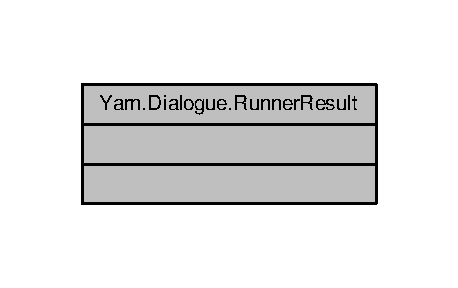
\includegraphics[width=220pt]{a00632}
\end{center}
\end{figure}


\subsection{Detailed Description}
Represents something for the end user (\char`\"{}client\char`\"{}) of the \hyperlink{a00092}{Dialogue} class to do. 

Definition at line 140 of file Dialogue.\-cs.



The documentation for this class was generated from the following file\-:\begin{DoxyCompactItemize}
\item 
Yarn\-Spinner/\hyperlink{a00305}{Dialogue.\-cs}\end{DoxyCompactItemize}

\hypertarget{a00157}{\section{System.\-Reflection.\-Type\-Info Class Reference}
\label{a00157}\index{System.\-Reflection.\-Type\-Info@{System.\-Reflection.\-Type\-Info}}
}


Collaboration diagram for System.\-Reflection.\-Type\-Info\-:
\nopagebreak
\begin{figure}[H]
\begin{center}
\leavevmode
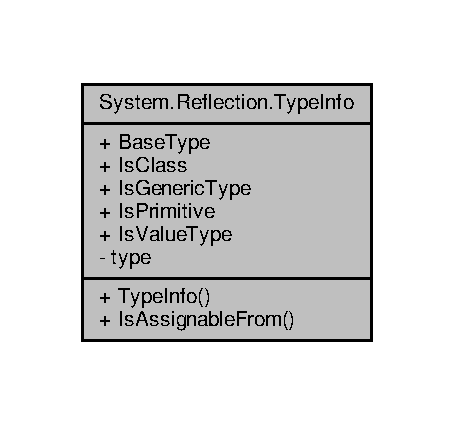
\includegraphics[width=218pt]{dd/d4d/a00519}
\end{center}
\end{figure}
\subsection*{Public Member Functions}
\begin{DoxyCompactItemize}
\item 
\hyperlink{a00157_ae2bbf4462c274977b6df5c994808cc39}{Type\-Info} (Type \hyperlink{a00157_a71c4f4b000d08808c8965222d4ba1b8d}{type})
\item 
bool \hyperlink{a00157_a8c74647f572e998dd7e843a752d5234d}{Is\-Assignable\-From} (\hyperlink{a00157}{Type\-Info} type\-Info)
\end{DoxyCompactItemize}
\subsection*{Public Attributes}
\begin{DoxyCompactItemize}
\item 
Type \hyperlink{a00157_a8bb78c2b0377f57dba1a3e2031216029}{Base\-Type} =$>$ type.\-Base\-Type
\item 
bool \hyperlink{a00157_a6ae2d0f4c557010a075a6fecab18fbb5}{Is\-Class} =$>$ type.\-Is\-Class
\item 
bool \hyperlink{a00157_a6a532f6a581b3280d1837fc242f314af}{Is\-Generic\-Type} =$>$ type.\-Is\-Generic\-Type
\item 
bool \hyperlink{a00157_ab38ba26ebc21ec6fb908b74eede99a5c}{Is\-Primitive} =$>$ type.\-Is\-Primitive
\item 
bool \hyperlink{a00157_ae2255904b8743c47a185d62909404aed}{Is\-Value\-Type} =$>$ type.\-Is\-Value\-Type
\end{DoxyCompactItemize}
\subsection*{Private Attributes}
\begin{DoxyCompactItemize}
\item 
readonly Type \hyperlink{a00157_a71c4f4b000d08808c8965222d4ba1b8d}{type}
\end{DoxyCompactItemize}


\subsection{Detailed Description}


\subsection{Constructor \& Destructor Documentation}
\hypertarget{a00157_ae2bbf4462c274977b6df5c994808cc39}{\index{System\-::\-Reflection\-::\-Type\-Info@{System\-::\-Reflection\-::\-Type\-Info}!Type\-Info@{Type\-Info}}
\index{Type\-Info@{Type\-Info}!System::Reflection::TypeInfo@{System\-::\-Reflection\-::\-Type\-Info}}
\subsubsection[{Type\-Info}]{\setlength{\rightskip}{0pt plus 5cm}System.\-Reflection.\-Type\-Info.\-Type\-Info (
\begin{DoxyParamCaption}
\item[{Type}]{type}
\end{DoxyParamCaption}
)}}\label{a00157_ae2bbf4462c274977b6df5c994808cc39}

\begin{DoxyCode}
21         \{
22             this.type = \hyperlink{a00157_a71c4f4b000d08808c8965222d4ba1b8d}{type};
23         \}
\end{DoxyCode}


\subsection{Member Function Documentation}
\hypertarget{a00157_a8c74647f572e998dd7e843a752d5234d}{\index{System\-::\-Reflection\-::\-Type\-Info@{System\-::\-Reflection\-::\-Type\-Info}!Is\-Assignable\-From@{Is\-Assignable\-From}}
\index{Is\-Assignable\-From@{Is\-Assignable\-From}!System::Reflection::TypeInfo@{System\-::\-Reflection\-::\-Type\-Info}}
\subsubsection[{Is\-Assignable\-From}]{\setlength{\rightskip}{0pt plus 5cm}bool System.\-Reflection.\-Type\-Info.\-Is\-Assignable\-From (
\begin{DoxyParamCaption}
\item[{{\bf Type\-Info}}]{type\-Info}
\end{DoxyParamCaption}
)}}\label{a00157_a8c74647f572e998dd7e843a752d5234d}

\begin{DoxyCode}
26         \{
27             \textcolor{keywordflow}{return} type.IsAssignableFrom( typeInfo.type );
28         \}
\end{DoxyCode}


\subsection{Member Data Documentation}
\hypertarget{a00157_a8bb78c2b0377f57dba1a3e2031216029}{\index{System\-::\-Reflection\-::\-Type\-Info@{System\-::\-Reflection\-::\-Type\-Info}!Base\-Type@{Base\-Type}}
\index{Base\-Type@{Base\-Type}!System::Reflection::TypeInfo@{System\-::\-Reflection\-::\-Type\-Info}}
\subsubsection[{Base\-Type}]{\setlength{\rightskip}{0pt plus 5cm}Type System.\-Reflection.\-Type\-Info.\-Base\-Type =$>$ type.\-Base\-Type}}\label{a00157_a8bb78c2b0377f57dba1a3e2031216029}
\hypertarget{a00157_a6ae2d0f4c557010a075a6fecab18fbb5}{\index{System\-::\-Reflection\-::\-Type\-Info@{System\-::\-Reflection\-::\-Type\-Info}!Is\-Class@{Is\-Class}}
\index{Is\-Class@{Is\-Class}!System::Reflection::TypeInfo@{System\-::\-Reflection\-::\-Type\-Info}}
\subsubsection[{Is\-Class}]{\setlength{\rightskip}{0pt plus 5cm}bool System.\-Reflection.\-Type\-Info.\-Is\-Class =$>$ type.\-Is\-Class}}\label{a00157_a6ae2d0f4c557010a075a6fecab18fbb5}
\hypertarget{a00157_a6a532f6a581b3280d1837fc242f314af}{\index{System\-::\-Reflection\-::\-Type\-Info@{System\-::\-Reflection\-::\-Type\-Info}!Is\-Generic\-Type@{Is\-Generic\-Type}}
\index{Is\-Generic\-Type@{Is\-Generic\-Type}!System::Reflection::TypeInfo@{System\-::\-Reflection\-::\-Type\-Info}}
\subsubsection[{Is\-Generic\-Type}]{\setlength{\rightskip}{0pt plus 5cm}bool System.\-Reflection.\-Type\-Info.\-Is\-Generic\-Type =$>$ type.\-Is\-Generic\-Type}}\label{a00157_a6a532f6a581b3280d1837fc242f314af}
\hypertarget{a00157_ab38ba26ebc21ec6fb908b74eede99a5c}{\index{System\-::\-Reflection\-::\-Type\-Info@{System\-::\-Reflection\-::\-Type\-Info}!Is\-Primitive@{Is\-Primitive}}
\index{Is\-Primitive@{Is\-Primitive}!System::Reflection::TypeInfo@{System\-::\-Reflection\-::\-Type\-Info}}
\subsubsection[{Is\-Primitive}]{\setlength{\rightskip}{0pt plus 5cm}bool System.\-Reflection.\-Type\-Info.\-Is\-Primitive =$>$ type.\-Is\-Primitive}}\label{a00157_ab38ba26ebc21ec6fb908b74eede99a5c}
\hypertarget{a00157_ae2255904b8743c47a185d62909404aed}{\index{System\-::\-Reflection\-::\-Type\-Info@{System\-::\-Reflection\-::\-Type\-Info}!Is\-Value\-Type@{Is\-Value\-Type}}
\index{Is\-Value\-Type@{Is\-Value\-Type}!System::Reflection::TypeInfo@{System\-::\-Reflection\-::\-Type\-Info}}
\subsubsection[{Is\-Value\-Type}]{\setlength{\rightskip}{0pt plus 5cm}bool System.\-Reflection.\-Type\-Info.\-Is\-Value\-Type =$>$ type.\-Is\-Value\-Type}}\label{a00157_ae2255904b8743c47a185d62909404aed}
\hypertarget{a00157_a71c4f4b000d08808c8965222d4ba1b8d}{\index{System\-::\-Reflection\-::\-Type\-Info@{System\-::\-Reflection\-::\-Type\-Info}!type@{type}}
\index{type@{type}!System::Reflection::TypeInfo@{System\-::\-Reflection\-::\-Type\-Info}}
\subsubsection[{type}]{\setlength{\rightskip}{0pt plus 5cm}readonly Type System.\-Reflection.\-Type\-Info.\-type\hspace{0.3cm}{\ttfamily [private]}}}\label{a00157_a71c4f4b000d08808c8965222d4ba1b8d}


The documentation for this class was generated from the following file\-:\begin{DoxyCompactItemize}
\item 
packages/\-Csv\-Helper.\-2.\-16.\-0.\-0/src/\-Csv\-Helper/\-Core\-Fx\-Compatibility/\hyperlink{a00196}{Type\-Info.\-cs}\end{DoxyCompactItemize}

\hypertarget{a00158}{\section{Csv\-Helper.\-Type\-Conversion.\-S\-Byte\-Converter Class Reference}
\label{a00158}\index{Csv\-Helper.\-Type\-Conversion.\-S\-Byte\-Converter@{Csv\-Helper.\-Type\-Conversion.\-S\-Byte\-Converter}}
}


Converts a S\-Byte to and from a string.  




Inheritance diagram for Csv\-Helper.\-Type\-Conversion.\-S\-Byte\-Converter\-:
\nopagebreak
\begin{figure}[H]
\begin{center}
\leavevmode
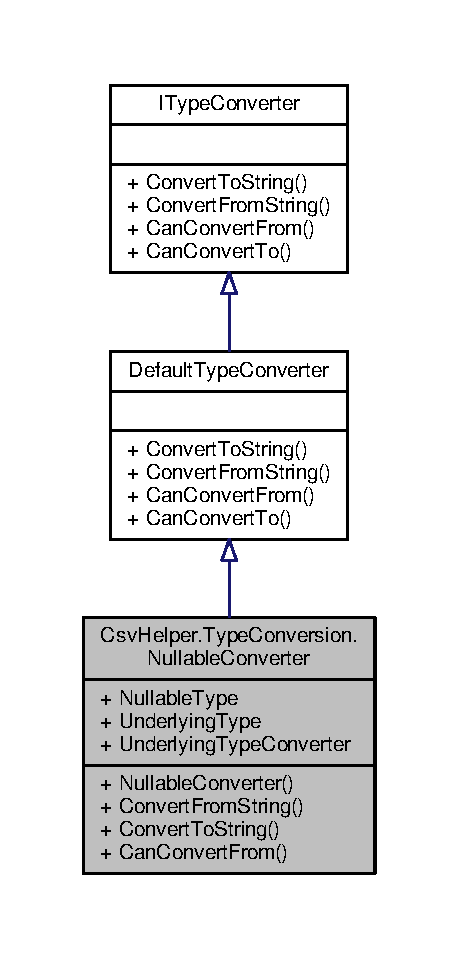
\includegraphics[width=220pt]{a00560}
\end{center}
\end{figure}


Collaboration diagram for Csv\-Helper.\-Type\-Conversion.\-S\-Byte\-Converter\-:
\nopagebreak
\begin{figure}[H]
\begin{center}
\leavevmode
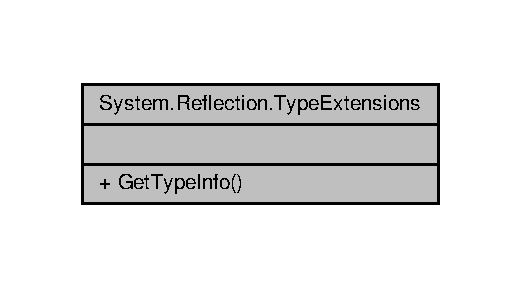
\includegraphics[width=220pt]{a00561}
\end{center}
\end{figure}
\subsection*{Public Member Functions}
\begin{DoxyCompactItemize}
\item 
override object \hyperlink{a00158_ad16aeb03f418c89b3f78e95b46a46b40}{Convert\-From\-String} (\hyperlink{a00178}{Type\-Converter\-Options} options, string text)
\begin{DoxyCompactList}\small\item\em Converts the string to an object. \end{DoxyCompactList}\item 
override bool \hyperlink{a00158_a8f6d23460e0ddfe883cc06ded76bf633}{Can\-Convert\-From} (System.\-Type type)
\begin{DoxyCompactList}\small\item\em Determines whether this instance \mbox{[}can convert from\mbox{]} the specified type. \end{DoxyCompactList}\item 
virtual string \hyperlink{a00088_a36cb2f9b24f15a671293f3a722324c27}{Convert\-To\-String} (\hyperlink{a00178}{Type\-Converter\-Options} options, object value)
\begin{DoxyCompactList}\small\item\em Converts the object to a string. \end{DoxyCompactList}\item 
virtual bool \hyperlink{a00088_a470d21adaa704eb281250dbd112ff91a}{Can\-Convert\-From} (Type type)
\begin{DoxyCompactList}\small\item\em Determines whether this instance \mbox{[}can convert from\mbox{]} the specified type. \end{DoxyCompactList}\item 
virtual bool \hyperlink{a00088_acb65bd8c8199d88d5b1629ae35d18514}{Can\-Convert\-To} (Type type)
\begin{DoxyCompactList}\small\item\em Determines whether this instance \mbox{[}can convert to\mbox{]} the specified type. \end{DoxyCompactList}\end{DoxyCompactItemize}


\subsection{Detailed Description}
Converts a S\-Byte to and from a string. 



Definition at line 12 of file S\-Byte\-Converter.\-cs.



\subsection{Member Function Documentation}
\hypertarget{a00158_a8f6d23460e0ddfe883cc06ded76bf633}{\index{Csv\-Helper\-::\-Type\-Conversion\-::\-S\-Byte\-Converter@{Csv\-Helper\-::\-Type\-Conversion\-::\-S\-Byte\-Converter}!Can\-Convert\-From@{Can\-Convert\-From}}
\index{Can\-Convert\-From@{Can\-Convert\-From}!CsvHelper::TypeConversion::SByteConverter@{Csv\-Helper\-::\-Type\-Conversion\-::\-S\-Byte\-Converter}}
\subsubsection[{Can\-Convert\-From}]{\setlength{\rightskip}{0pt plus 5cm}override bool Csv\-Helper.\-Type\-Conversion.\-S\-Byte\-Converter.\-Can\-Convert\-From (
\begin{DoxyParamCaption}
\item[{System.\-Type}]{type}
\end{DoxyParamCaption}
)}}\label{a00158_a8f6d23460e0ddfe883cc06ded76bf633}


Determines whether this instance \mbox{[}can convert from\mbox{]} the specified type. 


\begin{DoxyParams}{Parameters}
{\em type} & The type.\\
\hline
\end{DoxyParams}
\begin{DoxyReturn}{Returns}
{\ttfamily true} if this instance \mbox{[}can convert from\mbox{]} the specified type; otherwise, {\ttfamily false}. 
\end{DoxyReturn}


Definition at line 40 of file S\-Byte\-Converter.\-cs.


\begin{DoxyCode}
41         \{
42             \textcolor{comment}{// We only care about strings.}
43             \textcolor{keywordflow}{return} type == typeof( \textcolor{keywordtype}{string} );
44         \}
\end{DoxyCode}
\hypertarget{a00088_a470d21adaa704eb281250dbd112ff91a}{\index{Csv\-Helper\-::\-Type\-Conversion\-::\-S\-Byte\-Converter@{Csv\-Helper\-::\-Type\-Conversion\-::\-S\-Byte\-Converter}!Can\-Convert\-From@{Can\-Convert\-From}}
\index{Can\-Convert\-From@{Can\-Convert\-From}!CsvHelper::TypeConversion::SByteConverter@{Csv\-Helper\-::\-Type\-Conversion\-::\-S\-Byte\-Converter}}
\subsubsection[{Can\-Convert\-From}]{\setlength{\rightskip}{0pt plus 5cm}virtual bool Csv\-Helper.\-Type\-Conversion.\-Default\-Type\-Converter.\-Can\-Convert\-From (
\begin{DoxyParamCaption}
\item[{Type}]{type}
\end{DoxyParamCaption}
)\hspace{0.3cm}{\ttfamily [virtual]}, {\ttfamily [inherited]}}}\label{a00088_a470d21adaa704eb281250dbd112ff91a}


Determines whether this instance \mbox{[}can convert from\mbox{]} the specified type. 


\begin{DoxyParams}{Parameters}
{\em type} & The type.\\
\hline
\end{DoxyParams}
\begin{DoxyReturn}{Returns}
{\ttfamily true} if this instance \mbox{[}can convert from\mbox{]} the specified type; otherwise, {\ttfamily false}. 
\end{DoxyReturn}


Implements \hyperlink{a00123_ae1ad863656f4fa96bd846a41344c9349}{Csv\-Helper.\-Type\-Conversion.\-I\-Type\-Converter}.



Reimplemented in \hyperlink{a00142_ab9761a9f96be2b41103bb1313611d6f9}{Csv\-Helper.\-Type\-Conversion.\-Nullable\-Converter}, \hyperlink{a00045_a0be20573af4ee53409bb437125a64268}{Csv\-Helper.\-Type\-Conversion.\-Boolean\-Converter}, \hyperlink{a00098_a31af8209aad64ed11d949586075c244a}{Csv\-Helper.\-Type\-Conversion.\-Enum\-Converter}, \hyperlink{a00099_af66a7c67041f4c8061aa66e9e36359cf}{Csv\-Helper.\-Type\-Conversion.\-Enumerable\-Converter}, \hyperlink{a00085_a82a8cf4b77600ef49da60deb0c24a708}{Csv\-Helper.\-Type\-Conversion.\-Date\-Time\-Offset\-Converter}, \hyperlink{a00084_af44239d3bd014b1423fa80f7440bbd25}{Csv\-Helper.\-Type\-Conversion.\-Date\-Time\-Converter}, \hyperlink{a00046_a74a66b405f6c18e69b9fd23a1dea91b0}{Csv\-Helper.\-Type\-Conversion.\-Byte\-Converter}, and \hyperlink{a00172_ae3f8d46f5176d2ae08ac3fcdda1951e7}{Csv\-Helper.\-Type\-Conversion.\-Time\-Span\-Converter}.



Definition at line 55 of file Default\-Type\-Converter.\-cs.


\begin{DoxyCode}
56         \{
57             \textcolor{comment}{// The default convert doesn't know how to}
58             \textcolor{comment}{// convert from any type.}
59             \textcolor{keywordflow}{return} \textcolor{keyword}{false};
60         \}
\end{DoxyCode}
\hypertarget{a00088_acb65bd8c8199d88d5b1629ae35d18514}{\index{Csv\-Helper\-::\-Type\-Conversion\-::\-S\-Byte\-Converter@{Csv\-Helper\-::\-Type\-Conversion\-::\-S\-Byte\-Converter}!Can\-Convert\-To@{Can\-Convert\-To}}
\index{Can\-Convert\-To@{Can\-Convert\-To}!CsvHelper::TypeConversion::SByteConverter@{Csv\-Helper\-::\-Type\-Conversion\-::\-S\-Byte\-Converter}}
\subsubsection[{Can\-Convert\-To}]{\setlength{\rightskip}{0pt plus 5cm}virtual bool Csv\-Helper.\-Type\-Conversion.\-Default\-Type\-Converter.\-Can\-Convert\-To (
\begin{DoxyParamCaption}
\item[{Type}]{type}
\end{DoxyParamCaption}
)\hspace{0.3cm}{\ttfamily [virtual]}, {\ttfamily [inherited]}}}\label{a00088_acb65bd8c8199d88d5b1629ae35d18514}


Determines whether this instance \mbox{[}can convert to\mbox{]} the specified type. 


\begin{DoxyParams}{Parameters}
{\em type} & The type.\\
\hline
\end{DoxyParams}
\begin{DoxyReturn}{Returns}
{\ttfamily true} if this instance \mbox{[}can convert to\mbox{]} the specified type; otherwise, {\ttfamily false}. 
\end{DoxyReturn}


Implements \hyperlink{a00123_a168b03dad37fcb6882101c93deac8111}{Csv\-Helper.\-Type\-Conversion.\-I\-Type\-Converter}.



Reimplemented in \hyperlink{a00099_a44d625b44f770b945a29cd89e399f90f}{Csv\-Helper.\-Type\-Conversion.\-Enumerable\-Converter}.



Definition at line 69 of file Default\-Type\-Converter.\-cs.


\begin{DoxyCode}
70         \{
71             \textcolor{comment}{// We only care about strings.}
72             \textcolor{keywordflow}{return} type == typeof( \textcolor{keywordtype}{string} );
73         \}
\end{DoxyCode}
\hypertarget{a00158_ad16aeb03f418c89b3f78e95b46a46b40}{\index{Csv\-Helper\-::\-Type\-Conversion\-::\-S\-Byte\-Converter@{Csv\-Helper\-::\-Type\-Conversion\-::\-S\-Byte\-Converter}!Convert\-From\-String@{Convert\-From\-String}}
\index{Convert\-From\-String@{Convert\-From\-String}!CsvHelper::TypeConversion::SByteConverter@{Csv\-Helper\-::\-Type\-Conversion\-::\-S\-Byte\-Converter}}
\subsubsection[{Convert\-From\-String}]{\setlength{\rightskip}{0pt plus 5cm}override object Csv\-Helper.\-Type\-Conversion.\-S\-Byte\-Converter.\-Convert\-From\-String (
\begin{DoxyParamCaption}
\item[{{\bf Type\-Converter\-Options}}]{options, }
\item[{string}]{text}
\end{DoxyParamCaption}
)\hspace{0.3cm}{\ttfamily [virtual]}}}\label{a00158_ad16aeb03f418c89b3f78e95b46a46b40}


Converts the string to an object. 


\begin{DoxyParams}{Parameters}
{\em options} & The options to use when converting.\\
\hline
{\em text} & The string to convert to an object.\\
\hline
\end{DoxyParams}
\begin{DoxyReturn}{Returns}
The object created from the string.
\end{DoxyReturn}


Reimplemented from \hyperlink{a00088_a804ea00060e1de70e5151f90d3bfce9b}{Csv\-Helper.\-Type\-Conversion.\-Default\-Type\-Converter}.



Definition at line 20 of file S\-Byte\-Converter.\-cs.



References Csv\-Helper.\-Type\-Conversion.\-Type\-Converter\-Options.\-Culture\-Info.


\begin{DoxyCode}
21         \{
22             var numberStyle = options.NumberStyle ?? NumberStyles.Integer;
23 
24             sbyte sb;
25             \textcolor{keywordflow}{if}( sbyte.TryParse( text, numberStyle, options.CultureInfo, out sb ) )
26             \{
27                 \textcolor{keywordflow}{return} sb;
28             \}
29 
30             \textcolor{keywordflow}{return} base.ConvertFromString( options, text );
31         \}
\end{DoxyCode}
\hypertarget{a00088_a36cb2f9b24f15a671293f3a722324c27}{\index{Csv\-Helper\-::\-Type\-Conversion\-::\-S\-Byte\-Converter@{Csv\-Helper\-::\-Type\-Conversion\-::\-S\-Byte\-Converter}!Convert\-To\-String@{Convert\-To\-String}}
\index{Convert\-To\-String@{Convert\-To\-String}!CsvHelper::TypeConversion::SByteConverter@{Csv\-Helper\-::\-Type\-Conversion\-::\-S\-Byte\-Converter}}
\subsubsection[{Convert\-To\-String}]{\setlength{\rightskip}{0pt plus 5cm}virtual string Csv\-Helper.\-Type\-Conversion.\-Default\-Type\-Converter.\-Convert\-To\-String (
\begin{DoxyParamCaption}
\item[{{\bf Type\-Converter\-Options}}]{options, }
\item[{object}]{value}
\end{DoxyParamCaption}
)\hspace{0.3cm}{\ttfamily [virtual]}, {\ttfamily [inherited]}}}\label{a00088_a36cb2f9b24f15a671293f3a722324c27}


Converts the object to a string. 


\begin{DoxyParams}{Parameters}
{\em options} & The options to use when converting.\\
\hline
{\em value} & The object to convert to a string.\\
\hline
\end{DoxyParams}
\begin{DoxyReturn}{Returns}
The string representation of the object.
\end{DoxyReturn}


Implements \hyperlink{a00123_a90c465c63dbcf913f38aa878f35e77c7}{Csv\-Helper.\-Type\-Conversion.\-I\-Type\-Converter}.



Reimplemented in \hyperlink{a00142_a7205cdb61d2d119582958232b3e63109}{Csv\-Helper.\-Type\-Conversion.\-Nullable\-Converter}, and \hyperlink{a00099_a7e07e9532857d748654d37db590a0e11}{Csv\-Helper.\-Type\-Conversion.\-Enumerable\-Converter}.



Definition at line 21 of file Default\-Type\-Converter.\-cs.


\begin{DoxyCode}
22         \{
23             \textcolor{keywordflow}{if}( value == null )
24             \{
25                 \textcolor{keywordflow}{return} string.Empty;
26             \}
27 
28             var formattable = value as IFormattable;
29             \textcolor{keywordflow}{if}( formattable != null )
30             \{
31                 \textcolor{keywordflow}{return} formattable.ToString( options.Format, options.CultureInfo );
32             \}
33 
34             \textcolor{keywordflow}{return} value.ToString();
35         \}
\end{DoxyCode}


The documentation for this class was generated from the following file\-:\begin{DoxyCompactItemize}
\item 
packages/\-Csv\-Helper.\-2.\-16.\-0.\-0/src/\-Csv\-Helper/\-Type\-Conversion/\hyperlink{a00277}{S\-Byte\-Converter.\-cs}\end{DoxyCompactItemize}

\chapter{Class Documentation}
\hypertarget{a00019}{\section{Yarn.\-Parser.\-Assignment\-Statement Class Reference}
\label{a00019}\index{Yarn.\-Parser.\-Assignment\-Statement@{Yarn.\-Parser.\-Assignment\-Statement}}
}


Inheritance diagram for Yarn.\-Parser.\-Assignment\-Statement\-:
\nopagebreak
\begin{figure}[H]
\begin{center}
\leavevmode
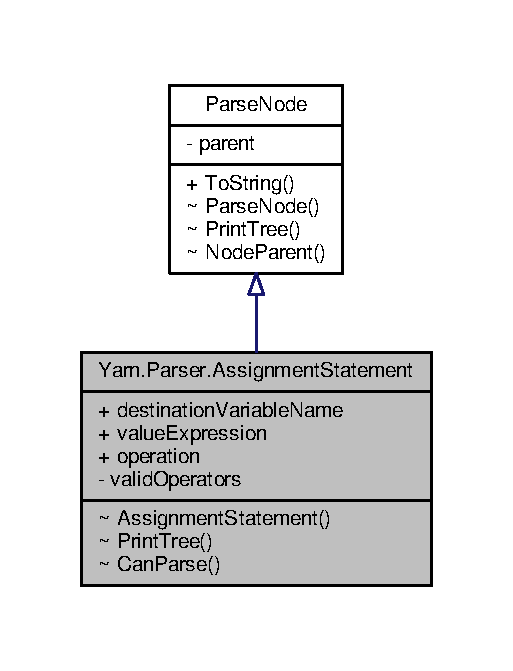
\includegraphics[width=246pt]{d9/d39/a00257}
\end{center}
\end{figure}


Collaboration diagram for Yarn.\-Parser.\-Assignment\-Statement\-:
\nopagebreak
\begin{figure}[H]
\begin{center}
\leavevmode
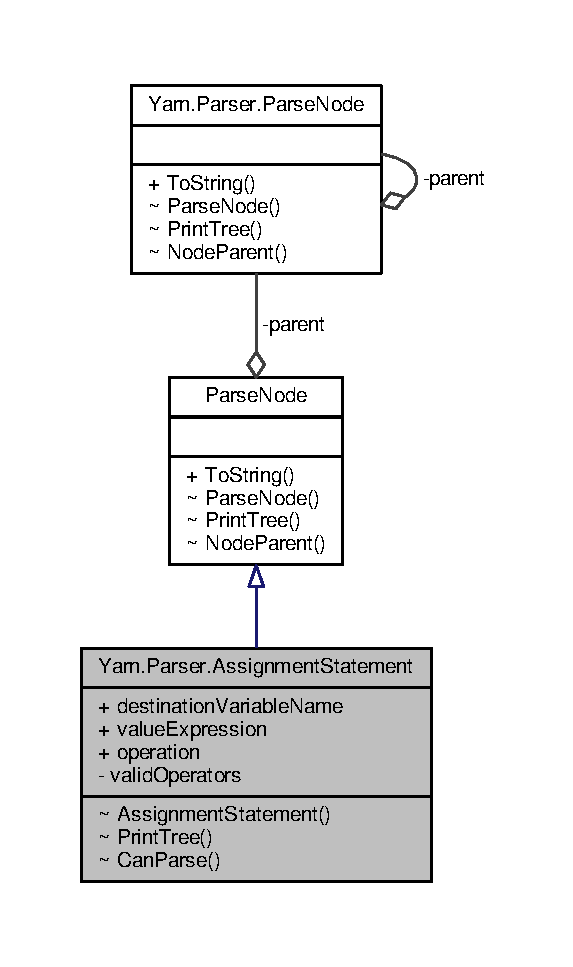
\includegraphics[width=275pt]{d7/d2f/a00258}
\end{center}
\end{figure}
\subsection*{Public Member Functions}
\begin{DoxyCompactItemize}
\item 
override string \hyperlink{a00063_a18c67cb16090d0889bb9d6c8c6c565f8}{To\-String} ()
\end{DoxyCompactItemize}
\subsection*{Package Functions}
\begin{DoxyCompactItemize}
\item 
\hyperlink{a00019_a34d41e545770d5f41542253d0bb4f8b3}{Assignment\-Statement} (\hyperlink{a00063}{Parse\-Node} \hyperlink{a00063_af313a82103fcc2ff5a177dbb06b92f7b}{parent}, \hyperlink{a00064}{Parser} p)
\item 
override string \hyperlink{a00019_accb9ddcb472eb035a65188c857b8efd8}{Print\-Tree} (int indent\-Level)
\item 
\hyperlink{a00054}{Node} \hyperlink{a00063_a580e520a29444fc23ac3660cbe514a09}{Node\-Parent} ()
\end{DoxyCompactItemize}
\subsection*{Static Package Functions}
\begin{DoxyCompactItemize}
\item 
static bool \hyperlink{a00019_a4f021e4c835e429ed5b5bb504a5acf39}{Can\-Parse} (\hyperlink{a00064}{Parser} p)
\end{DoxyCompactItemize}
\subsection*{Properties}
\begin{DoxyCompactItemize}
\item 
string \hyperlink{a00019_a4e764622b716a4138d1fd9e005c41336}{destination\-Variable\-Name}\hspace{0.3cm}{\ttfamily  \mbox{[}get, set\mbox{]}}
\item 
\hyperlink{a00040}{Expression} \hyperlink{a00019_a7ada366012cacd98436db80227ee65f5}{value\-Expression}\hspace{0.3cm}{\ttfamily  \mbox{[}get, set\mbox{]}}
\item 
\hyperlink{a00026_a301aa7c866593a5b625a8fc158bbeace}{Token\-Type} \hyperlink{a00019_a896df0f23b44e9f20036150b3527d9e5}{operation}\hspace{0.3cm}{\ttfamily  \mbox{[}get, set\mbox{]}}
\end{DoxyCompactItemize}
\subsection*{Static Private Attributes}
\begin{DoxyCompactItemize}
\item 
static \hyperlink{a00026_a301aa7c866593a5b625a8fc158bbeace}{Token\-Type}\mbox{[}$\,$\mbox{]} \hyperlink{a00019_af3d393da2f684272251805d3471b6c7a}{valid\-Operators}
\end{DoxyCompactItemize}


\subsection{Detailed Description}


\subsection{Constructor \& Destructor Documentation}
\hypertarget{a00019_a34d41e545770d5f41542253d0bb4f8b3}{\index{Yarn\-::\-Parser\-::\-Assignment\-Statement@{Yarn\-::\-Parser\-::\-Assignment\-Statement}!Assignment\-Statement@{Assignment\-Statement}}
\index{Assignment\-Statement@{Assignment\-Statement}!Yarn::Parser::AssignmentStatement@{Yarn\-::\-Parser\-::\-Assignment\-Statement}}
\subsubsection[{Assignment\-Statement}]{\setlength{\rightskip}{0pt plus 5cm}Yarn.\-Parser.\-Assignment\-Statement.\-Assignment\-Statement (
\begin{DoxyParamCaption}
\item[{{\bf Parse\-Node}}]{parent, }
\item[{{\bf Parser}}]{p}
\end{DoxyParamCaption}
)\hspace{0.3cm}{\ttfamily [package]}}}\label{a00019_a34d41e545770d5f41542253d0bb4f8b3}

\begin{DoxyCode}
1098                                                                      : base(
      \hyperlink{a00063_af313a82103fcc2ff5a177dbb06b92f7b}{parent}, p) \{
1099 
1100                 p.ExpectSymbol(TokenType.BeginCommand);
1101                 p.ExpectSymbol(TokenType.Set);
1102                 \hyperlink{a00019_a4e764622b716a4138d1fd9e005c41336}{destinationVariableName} = p.ExpectSymbol(TokenType.Variable).value 
      as \textcolor{keywordtype}{string};
1103                 \hyperlink{a00019_a896df0f23b44e9f20036150b3527d9e5}{operation} = p.ExpectSymbol(\hyperlink{a00019_af3d393da2f684272251805d3471b6c7a}{validOperators}).type;
1104                 \hyperlink{a00019_a7ada366012cacd98436db80227ee65f5}{valueExpression} = Expression.Parse(\textcolor{keyword}{this}, p);
1105                 p.ExpectSymbol(TokenType.EndCommand);
1106 
1107             \}
\end{DoxyCode}


\subsection{Member Function Documentation}
\hypertarget{a00019_a4f021e4c835e429ed5b5bb504a5acf39}{\index{Yarn\-::\-Parser\-::\-Assignment\-Statement@{Yarn\-::\-Parser\-::\-Assignment\-Statement}!Can\-Parse@{Can\-Parse}}
\index{Can\-Parse@{Can\-Parse}!Yarn::Parser::AssignmentStatement@{Yarn\-::\-Parser\-::\-Assignment\-Statement}}
\subsubsection[{Can\-Parse}]{\setlength{\rightskip}{0pt plus 5cm}static bool Yarn.\-Parser.\-Assignment\-Statement.\-Can\-Parse (
\begin{DoxyParamCaption}
\item[{{\bf Parser}}]{p}
\end{DoxyParamCaption}
)\hspace{0.3cm}{\ttfamily [static]}, {\ttfamily [package]}}}\label{a00019_a4f021e4c835e429ed5b5bb504a5acf39}

\begin{DoxyCode}
1080             \{
1081                 \textcolor{keywordflow}{return} p.NextSymbolsAre (TokenType.BeginCommand, TokenType.Set);
1082             \}
\end{DoxyCode}
\hypertarget{a00063_a580e520a29444fc23ac3660cbe514a09}{\index{Yarn\-::\-Parser\-::\-Assignment\-Statement@{Yarn\-::\-Parser\-::\-Assignment\-Statement}!Node\-Parent@{Node\-Parent}}
\index{Node\-Parent@{Node\-Parent}!Yarn::Parser::AssignmentStatement@{Yarn\-::\-Parser\-::\-Assignment\-Statement}}
\subsubsection[{Node\-Parent}]{\setlength{\rightskip}{0pt plus 5cm}{\bf Node} Yarn.\-Parser.\-Parse\-Node.\-Node\-Parent (
\begin{DoxyParamCaption}
{}
\end{DoxyParamCaption}
)\hspace{0.3cm}{\ttfamily [package]}, {\ttfamily [inherited]}}}\label{a00063_a580e520a29444fc23ac3660cbe514a09}

\begin{DoxyCode}
116                                        \{
117                 var node = \textcolor{keyword}{this};
118 
119                 \textcolor{keywordflow}{do} \{
120                     \textcolor{keywordflow}{if} (node is Node) \{
121                         \textcolor{keywordflow}{return} node as Node;
122                     \}
123                     node = node.parent;
124                 \} \textcolor{keywordflow}{while} (node 
125                     != null);                   
126 
127                 \textcolor{keywordflow}{return} null;
128             \}
\end{DoxyCode}
\hypertarget{a00019_accb9ddcb472eb035a65188c857b8efd8}{\index{Yarn\-::\-Parser\-::\-Assignment\-Statement@{Yarn\-::\-Parser\-::\-Assignment\-Statement}!Print\-Tree@{Print\-Tree}}
\index{Print\-Tree@{Print\-Tree}!Yarn::Parser::AssignmentStatement@{Yarn\-::\-Parser\-::\-Assignment\-Statement}}
\subsubsection[{Print\-Tree}]{\setlength{\rightskip}{0pt plus 5cm}override string Yarn.\-Parser.\-Assignment\-Statement.\-Print\-Tree (
\begin{DoxyParamCaption}
\item[{int}]{indent\-Level}
\end{DoxyParamCaption}
)\hspace{0.3cm}{\ttfamily [package]}, {\ttfamily [virtual]}}}\label{a00019_accb9ddcb472eb035a65188c857b8efd8}


Implements \hyperlink{a00063_a0d6611653f20c2e4d90a97a96c657137}{Yarn.\-Parser.\-Parse\-Node}.


\begin{DoxyCode}
1110             \{
1111                 var sb = \textcolor{keyword}{new} StringBuilder ();
1112                 sb.Append (\hyperlink{a00064_aa8fa36b46de12a1c561d77b99c4b9ae3}{Tab}(indentLevel, \textcolor{stringliteral}{"Set:"}));
1113                 sb.Append (\hyperlink{a00064_aa8fa36b46de12a1c561d77b99c4b9ae3}{Tab}(indentLevel+1, \hyperlink{a00019_a4e764622b716a4138d1fd9e005c41336}{destinationVariableName}));
1114                 sb.Append (\hyperlink{a00064_aa8fa36b46de12a1c561d77b99c4b9ae3}{Tab} (indentLevel+1,  \hyperlink{a00019_a896df0f23b44e9f20036150b3527d9e5}{operation}.ToString()));
1115                 sb.Append (valueExpression.PrintTree (indentLevel + 1));
1116                 \textcolor{keywordflow}{return} sb.ToString ();
1117 
1118             \}
\end{DoxyCode}
\hypertarget{a00063_a18c67cb16090d0889bb9d6c8c6c565f8}{\index{Yarn\-::\-Parser\-::\-Assignment\-Statement@{Yarn\-::\-Parser\-::\-Assignment\-Statement}!To\-String@{To\-String}}
\index{To\-String@{To\-String}!Yarn::Parser::AssignmentStatement@{Yarn\-::\-Parser\-::\-Assignment\-Statement}}
\subsubsection[{To\-String}]{\setlength{\rightskip}{0pt plus 5cm}override string Yarn.\-Parser.\-Parse\-Node.\-To\-String (
\begin{DoxyParamCaption}
{}
\end{DoxyParamCaption}
)\hspace{0.3cm}{\ttfamily [inherited]}}}\label{a00063_a18c67cb16090d0889bb9d6c8c6c565f8}

\begin{DoxyCode}
111             \{
112                 \textcolor{keywordflow}{return} this.GetType ().Name;
113             \}
\end{DoxyCode}


\subsection{Member Data Documentation}
\hypertarget{a00019_af3d393da2f684272251805d3471b6c7a}{\index{Yarn\-::\-Parser\-::\-Assignment\-Statement@{Yarn\-::\-Parser\-::\-Assignment\-Statement}!valid\-Operators@{valid\-Operators}}
\index{valid\-Operators@{valid\-Operators}!Yarn::Parser::AssignmentStatement@{Yarn\-::\-Parser\-::\-Assignment\-Statement}}
\subsubsection[{valid\-Operators}]{\setlength{\rightskip}{0pt plus 5cm}{\bf Token\-Type} \mbox{[}$\,$\mbox{]} Yarn.\-Parser.\-Assignment\-Statement.\-valid\-Operators\hspace{0.3cm}{\ttfamily [static]}, {\ttfamily [private]}}}\label{a00019_af3d393da2f684272251805d3471b6c7a}
{\bfseries Initial value\-:}
\begin{DoxyCode}
= \{
                TokenType.EqualToOrAssign,
                TokenType.AddAssign,
                TokenType.MinusAssign,
                TokenType.DivideAssign,
                TokenType.MultiplyAssign
            \}
\end{DoxyCode}


\subsection{Property Documentation}
\hypertarget{a00019_a4e764622b716a4138d1fd9e005c41336}{\index{Yarn\-::\-Parser\-::\-Assignment\-Statement@{Yarn\-::\-Parser\-::\-Assignment\-Statement}!destination\-Variable\-Name@{destination\-Variable\-Name}}
\index{destination\-Variable\-Name@{destination\-Variable\-Name}!Yarn::Parser::AssignmentStatement@{Yarn\-::\-Parser\-::\-Assignment\-Statement}}
\subsubsection[{destination\-Variable\-Name}]{\setlength{\rightskip}{0pt plus 5cm}string Yarn.\-Parser.\-Assignment\-Statement.\-destination\-Variable\-Name\hspace{0.3cm}{\ttfamily [get]}, {\ttfamily [set]}, {\ttfamily [package]}}}\label{a00019_a4e764622b716a4138d1fd9e005c41336}
\hypertarget{a00019_a896df0f23b44e9f20036150b3527d9e5}{\index{Yarn\-::\-Parser\-::\-Assignment\-Statement@{Yarn\-::\-Parser\-::\-Assignment\-Statement}!operation@{operation}}
\index{operation@{operation}!Yarn::Parser::AssignmentStatement@{Yarn\-::\-Parser\-::\-Assignment\-Statement}}
\subsubsection[{operation}]{\setlength{\rightskip}{0pt plus 5cm}{\bf Token\-Type} Yarn.\-Parser.\-Assignment\-Statement.\-operation\hspace{0.3cm}{\ttfamily [get]}, {\ttfamily [set]}, {\ttfamily [package]}}}\label{a00019_a896df0f23b44e9f20036150b3527d9e5}
\hypertarget{a00019_a7ada366012cacd98436db80227ee65f5}{\index{Yarn\-::\-Parser\-::\-Assignment\-Statement@{Yarn\-::\-Parser\-::\-Assignment\-Statement}!value\-Expression@{value\-Expression}}
\index{value\-Expression@{value\-Expression}!Yarn::Parser::AssignmentStatement@{Yarn\-::\-Parser\-::\-Assignment\-Statement}}
\subsubsection[{value\-Expression}]{\setlength{\rightskip}{0pt plus 5cm}{\bf Expression} Yarn.\-Parser.\-Assignment\-Statement.\-value\-Expression\hspace{0.3cm}{\ttfamily [get]}, {\ttfamily [set]}, {\ttfamily [package]}}}\label{a00019_a7ada366012cacd98436db80227ee65f5}


The documentation for this class was generated from the following file\-:\begin{DoxyCompactItemize}
\item 
Yarn\-Spinner/\hyperlink{a00122}{Parser.\-cs}\end{DoxyCompactItemize}

\hypertarget{a00020}{\section{Yarn.\-Parser.\-Assignment\-Statement Class Reference}
\label{a00020}\index{Yarn.\-Parser.\-Assignment\-Statement@{Yarn.\-Parser.\-Assignment\-Statement}}
}


Inheritance diagram for Yarn.\-Parser.\-Assignment\-Statement\-:
\nopagebreak
\begin{figure}[H]
\begin{center}
\leavevmode
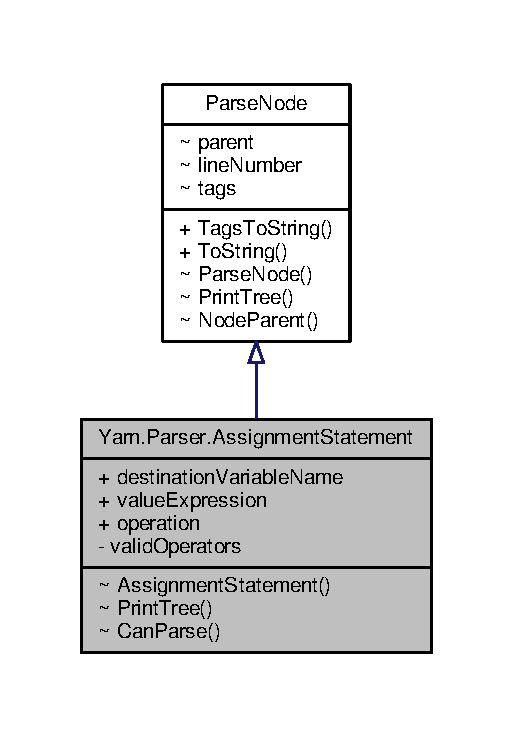
\includegraphics[width=246pt]{d0/dec/a00592}
\end{center}
\end{figure}


Collaboration diagram for Yarn.\-Parser.\-Assignment\-Statement\-:
\nopagebreak
\begin{figure}[H]
\begin{center}
\leavevmode
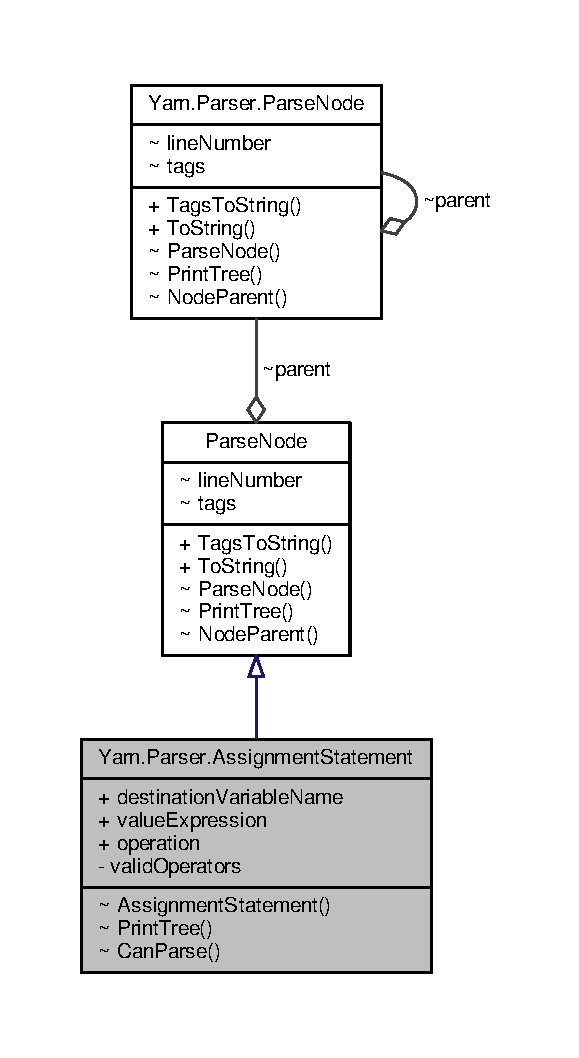
\includegraphics[width=278pt]{d2/da3/a00593}
\end{center}
\end{figure}
\subsection*{Public Member Functions}
\begin{DoxyCompactItemize}
\item 
string \hyperlink{a00122_a054f36c80d5eeacd569a8859f599af67}{Tags\-To\-String} (int indent\-Level)
\item 
override string \hyperlink{a00122_a18c67cb16090d0889bb9d6c8c6c565f8}{To\-String} ()
\end{DoxyCompactItemize}
\subsection*{Package Functions}
\begin{DoxyCompactItemize}
\item 
\hyperlink{a00020_a34d41e545770d5f41542253d0bb4f8b3}{Assignment\-Statement} (\hyperlink{a00122}{Parse\-Node} \hyperlink{a00122_af313a82103fcc2ff5a177dbb06b92f7b}{parent}, \hyperlink{a00123}{Parser} p)
\item 
override string \hyperlink{a00020_accb9ddcb472eb035a65188c857b8efd8}{Print\-Tree} (int indent\-Level)
\item 
\hyperlink{a00112}{Node} \hyperlink{a00122_a580e520a29444fc23ac3660cbe514a09}{Node\-Parent} ()
\end{DoxyCompactItemize}
\subsection*{Static Package Functions}
\begin{DoxyCompactItemize}
\item 
static bool \hyperlink{a00020_a4f021e4c835e429ed5b5bb504a5acf39}{Can\-Parse} (\hyperlink{a00123}{Parser} p)
\end{DoxyCompactItemize}
\subsection*{Package Attributes}
\begin{DoxyCompactItemize}
\item 
\hyperlink{a00122}{Parse\-Node} \hyperlink{a00122_af313a82103fcc2ff5a177dbb06b92f7b}{parent}
\item 
int \hyperlink{a00122_a18b493382de0fde5b4299c1bd2250075}{line\-Number}
\item 
string\mbox{[}$\,$\mbox{]} \hyperlink{a00122_a58b3a15788fd2d4127d73619dc6d04ae}{tags} = \{\}
\end{DoxyCompactItemize}
\subsection*{Properties}
\begin{DoxyCompactItemize}
\item 
string \hyperlink{a00020_a4e764622b716a4138d1fd9e005c41336}{destination\-Variable\-Name}\hspace{0.3cm}{\ttfamily  \mbox{[}get, set\mbox{]}}
\item 
\hyperlink{a00082}{Expression} \hyperlink{a00020_a7ada366012cacd98436db80227ee65f5}{value\-Expression}\hspace{0.3cm}{\ttfamily  \mbox{[}get, set\mbox{]}}
\item 
\hyperlink{a00031_a301aa7c866593a5b625a8fc158bbeace}{Token\-Type} \hyperlink{a00020_a896df0f23b44e9f20036150b3527d9e5}{operation}\hspace{0.3cm}{\ttfamily  \mbox{[}get, set\mbox{]}}
\end{DoxyCompactItemize}
\subsection*{Static Private Attributes}
\begin{DoxyCompactItemize}
\item 
static \hyperlink{a00031_a301aa7c866593a5b625a8fc158bbeace}{Token\-Type}\mbox{[}$\,$\mbox{]} \hyperlink{a00020_af3d393da2f684272251805d3471b6c7a}{valid\-Operators}
\end{DoxyCompactItemize}


\subsection{Detailed Description}


\subsection{Constructor \& Destructor Documentation}
\hypertarget{a00020_a34d41e545770d5f41542253d0bb4f8b3}{\index{Yarn\-::\-Parser\-::\-Assignment\-Statement@{Yarn\-::\-Parser\-::\-Assignment\-Statement}!Assignment\-Statement@{Assignment\-Statement}}
\index{Assignment\-Statement@{Assignment\-Statement}!Yarn::Parser::AssignmentStatement@{Yarn\-::\-Parser\-::\-Assignment\-Statement}}
\subsubsection[{Assignment\-Statement}]{\setlength{\rightskip}{0pt plus 5cm}Yarn.\-Parser.\-Assignment\-Statement.\-Assignment\-Statement (
\begin{DoxyParamCaption}
\item[{{\bf Parse\-Node}}]{parent, }
\item[{{\bf Parser}}]{p}
\end{DoxyParamCaption}
)\hspace{0.3cm}{\ttfamily [package]}}}\label{a00020_a34d41e545770d5f41542253d0bb4f8b3}

\begin{DoxyCode}
1176                                                                      : base(
      \hyperlink{a00122_af313a82103fcc2ff5a177dbb06b92f7b}{parent}, p) \{
1177 
1178                 p.ExpectSymbol(TokenType.BeginCommand);
1179                 p.ExpectSymbol(TokenType.Set);
1180                 \hyperlink{a00020_a4e764622b716a4138d1fd9e005c41336}{destinationVariableName} = p.ExpectSymbol(TokenType.Variable).value 
      as \textcolor{keywordtype}{string};
1181                 \hyperlink{a00020_a896df0f23b44e9f20036150b3527d9e5}{operation} = p.ExpectSymbol(\hyperlink{a00020_af3d393da2f684272251805d3471b6c7a}{validOperators}).type;
1182                 \hyperlink{a00020_a7ada366012cacd98436db80227ee65f5}{valueExpression} = Expression.Parse(\textcolor{keyword}{this}, p);
1183                 p.ExpectSymbol(TokenType.EndCommand);
1184 
1185             \}
\end{DoxyCode}


\subsection{Member Function Documentation}
\hypertarget{a00020_a4f021e4c835e429ed5b5bb504a5acf39}{\index{Yarn\-::\-Parser\-::\-Assignment\-Statement@{Yarn\-::\-Parser\-::\-Assignment\-Statement}!Can\-Parse@{Can\-Parse}}
\index{Can\-Parse@{Can\-Parse}!Yarn::Parser::AssignmentStatement@{Yarn\-::\-Parser\-::\-Assignment\-Statement}}
\subsubsection[{Can\-Parse}]{\setlength{\rightskip}{0pt plus 5cm}static bool Yarn.\-Parser.\-Assignment\-Statement.\-Can\-Parse (
\begin{DoxyParamCaption}
\item[{{\bf Parser}}]{p}
\end{DoxyParamCaption}
)\hspace{0.3cm}{\ttfamily [static]}, {\ttfamily [package]}}}\label{a00020_a4f021e4c835e429ed5b5bb504a5acf39}

\begin{DoxyCode}
1158             \{
1159                 \textcolor{keywordflow}{return} p.NextSymbolsAre (TokenType.BeginCommand, TokenType.Set);
1160             \}
\end{DoxyCode}
\hypertarget{a00122_a580e520a29444fc23ac3660cbe514a09}{\index{Yarn\-::\-Parser\-::\-Assignment\-Statement@{Yarn\-::\-Parser\-::\-Assignment\-Statement}!Node\-Parent@{Node\-Parent}}
\index{Node\-Parent@{Node\-Parent}!Yarn::Parser::AssignmentStatement@{Yarn\-::\-Parser\-::\-Assignment\-Statement}}
\subsubsection[{Node\-Parent}]{\setlength{\rightskip}{0pt plus 5cm}{\bf Node} Yarn.\-Parser.\-Parse\-Node.\-Node\-Parent (
\begin{DoxyParamCaption}
{}
\end{DoxyParamCaption}
)\hspace{0.3cm}{\ttfamily [package]}, {\ttfamily [inherited]}}}\label{a00122_a580e520a29444fc23ac3660cbe514a09}

\begin{DoxyCode}
144                                        \{
145                 var node = \textcolor{keyword}{this};
146 
147                 \textcolor{keywordflow}{do} \{
148                     \textcolor{keywordflow}{if} (node is Node) \{
149                         \textcolor{keywordflow}{return} node as Node;
150                     \}
151                     node = node.parent;
152                 \} \textcolor{keywordflow}{while} (node 
153                     != null);                   
154 
155                 \textcolor{keywordflow}{return} null;
156             \}
\end{DoxyCode}
\hypertarget{a00020_accb9ddcb472eb035a65188c857b8efd8}{\index{Yarn\-::\-Parser\-::\-Assignment\-Statement@{Yarn\-::\-Parser\-::\-Assignment\-Statement}!Print\-Tree@{Print\-Tree}}
\index{Print\-Tree@{Print\-Tree}!Yarn::Parser::AssignmentStatement@{Yarn\-::\-Parser\-::\-Assignment\-Statement}}
\subsubsection[{Print\-Tree}]{\setlength{\rightskip}{0pt plus 5cm}override string Yarn.\-Parser.\-Assignment\-Statement.\-Print\-Tree (
\begin{DoxyParamCaption}
\item[{int}]{indent\-Level}
\end{DoxyParamCaption}
)\hspace{0.3cm}{\ttfamily [package]}, {\ttfamily [virtual]}}}\label{a00020_accb9ddcb472eb035a65188c857b8efd8}


Implements \hyperlink{a00122_a0d6611653f20c2e4d90a97a96c657137}{Yarn.\-Parser.\-Parse\-Node}.


\begin{DoxyCode}
1188             \{
1189                 var sb = \textcolor{keyword}{new} StringBuilder ();
1190                 sb.Append (\hyperlink{a00123_aa8fa36b46de12a1c561d77b99c4b9ae3}{Tab}(indentLevel, \textcolor{stringliteral}{"Set:"}));
1191                 sb.Append (\hyperlink{a00123_aa8fa36b46de12a1c561d77b99c4b9ae3}{Tab}(indentLevel+1, \hyperlink{a00020_a4e764622b716a4138d1fd9e005c41336}{destinationVariableName}));
1192                 sb.Append (\hyperlink{a00123_aa8fa36b46de12a1c561d77b99c4b9ae3}{Tab} (indentLevel+1,  \hyperlink{a00020_a896df0f23b44e9f20036150b3527d9e5}{operation}.ToString()));
1193                 sb.Append (valueExpression.PrintTree (indentLevel + 1));
1194                 \textcolor{keywordflow}{return} sb.ToString ();
1195 
1196             \}
\end{DoxyCode}
\hypertarget{a00122_a054f36c80d5eeacd569a8859f599af67}{\index{Yarn\-::\-Parser\-::\-Assignment\-Statement@{Yarn\-::\-Parser\-::\-Assignment\-Statement}!Tags\-To\-String@{Tags\-To\-String}}
\index{Tags\-To\-String@{Tags\-To\-String}!Yarn::Parser::AssignmentStatement@{Yarn\-::\-Parser\-::\-Assignment\-Statement}}
\subsubsection[{Tags\-To\-String}]{\setlength{\rightskip}{0pt plus 5cm}string Yarn.\-Parser.\-Parse\-Node.\-Tags\-To\-String (
\begin{DoxyParamCaption}
\item[{int}]{indent\-Level}
\end{DoxyParamCaption}
)\hspace{0.3cm}{\ttfamily [inherited]}}}\label{a00122_a054f36c80d5eeacd569a8859f599af67}

\begin{DoxyCode}
122             \{
123                 \textcolor{keywordflow}{if} (\hyperlink{a00122_a58b3a15788fd2d4127d73619dc6d04ae}{tags}.Length > 0) \{
124                     var s = \textcolor{keyword}{new} StringBuilder ();
125 
126                     s.Append (\hyperlink{a00123_aa8fa36b46de12a1c561d77b99c4b9ae3}{Tab} (indentLevel + 1, \textcolor{stringliteral}{"Tags:"}));
127                     \textcolor{keywordflow}{foreach} (var tag \textcolor{keywordflow}{in} this.\hyperlink{a00122_a58b3a15788fd2d4127d73619dc6d04ae}{tags}) \{
128                         s.Append(\hyperlink{a00123_aa8fa36b46de12a1c561d77b99c4b9ae3}{Tab} (indentLevel + 2, \textcolor{stringliteral}{"#"} + tag));
129                     \}
130                     \textcolor{keywordflow}{return} s.ToString ();
131                 \} \textcolor{keywordflow}{else} \{
132                     \textcolor{keywordflow}{return} \textcolor{stringliteral}{""};
133                 \}
134 
135 
136             \}
\end{DoxyCode}
\hypertarget{a00122_a18c67cb16090d0889bb9d6c8c6c565f8}{\index{Yarn\-::\-Parser\-::\-Assignment\-Statement@{Yarn\-::\-Parser\-::\-Assignment\-Statement}!To\-String@{To\-String}}
\index{To\-String@{To\-String}!Yarn::Parser::AssignmentStatement@{Yarn\-::\-Parser\-::\-Assignment\-Statement}}
\subsubsection[{To\-String}]{\setlength{\rightskip}{0pt plus 5cm}override string Yarn.\-Parser.\-Parse\-Node.\-To\-String (
\begin{DoxyParamCaption}
{}
\end{DoxyParamCaption}
)\hspace{0.3cm}{\ttfamily [inherited]}}}\label{a00122_a18c67cb16090d0889bb9d6c8c6c565f8}

\begin{DoxyCode}
139             \{
140                 \textcolor{keywordflow}{return} this.GetType ().Name;
141             \}
\end{DoxyCode}


\subsection{Member Data Documentation}
\hypertarget{a00122_a18b493382de0fde5b4299c1bd2250075}{\index{Yarn\-::\-Parser\-::\-Assignment\-Statement@{Yarn\-::\-Parser\-::\-Assignment\-Statement}!line\-Number@{line\-Number}}
\index{line\-Number@{line\-Number}!Yarn::Parser::AssignmentStatement@{Yarn\-::\-Parser\-::\-Assignment\-Statement}}
\subsubsection[{line\-Number}]{\setlength{\rightskip}{0pt plus 5cm}int Yarn.\-Parser.\-Parse\-Node.\-line\-Number\hspace{0.3cm}{\ttfamily [package]}, {\ttfamily [inherited]}}}\label{a00122_a18b493382de0fde5b4299c1bd2250075}
\hypertarget{a00122_af313a82103fcc2ff5a177dbb06b92f7b}{\index{Yarn\-::\-Parser\-::\-Assignment\-Statement@{Yarn\-::\-Parser\-::\-Assignment\-Statement}!parent@{parent}}
\index{parent@{parent}!Yarn::Parser::AssignmentStatement@{Yarn\-::\-Parser\-::\-Assignment\-Statement}}
\subsubsection[{parent}]{\setlength{\rightskip}{0pt plus 5cm}{\bf Parse\-Node} Yarn.\-Parser.\-Parse\-Node.\-parent\hspace{0.3cm}{\ttfamily [package]}, {\ttfamily [inherited]}}}\label{a00122_af313a82103fcc2ff5a177dbb06b92f7b}
\hypertarget{a00122_a58b3a15788fd2d4127d73619dc6d04ae}{\index{Yarn\-::\-Parser\-::\-Assignment\-Statement@{Yarn\-::\-Parser\-::\-Assignment\-Statement}!tags@{tags}}
\index{tags@{tags}!Yarn::Parser::AssignmentStatement@{Yarn\-::\-Parser\-::\-Assignment\-Statement}}
\subsubsection[{tags}]{\setlength{\rightskip}{0pt plus 5cm}string \mbox{[}$\,$\mbox{]} Yarn.\-Parser.\-Parse\-Node.\-tags = \{\}\hspace{0.3cm}{\ttfamily [package]}, {\ttfamily [inherited]}}}\label{a00122_a58b3a15788fd2d4127d73619dc6d04ae}
\hypertarget{a00020_af3d393da2f684272251805d3471b6c7a}{\index{Yarn\-::\-Parser\-::\-Assignment\-Statement@{Yarn\-::\-Parser\-::\-Assignment\-Statement}!valid\-Operators@{valid\-Operators}}
\index{valid\-Operators@{valid\-Operators}!Yarn::Parser::AssignmentStatement@{Yarn\-::\-Parser\-::\-Assignment\-Statement}}
\subsubsection[{valid\-Operators}]{\setlength{\rightskip}{0pt plus 5cm}{\bf Token\-Type} \mbox{[}$\,$\mbox{]} Yarn.\-Parser.\-Assignment\-Statement.\-valid\-Operators\hspace{0.3cm}{\ttfamily [static]}, {\ttfamily [private]}}}\label{a00020_af3d393da2f684272251805d3471b6c7a}
{\bfseries Initial value\-:}
\begin{DoxyCode}
= \{
                TokenType.EqualToOrAssign,
                TokenType.AddAssign,
                TokenType.MinusAssign,
                TokenType.DivideAssign,
                TokenType.MultiplyAssign
            \}
\end{DoxyCode}


\subsection{Property Documentation}
\hypertarget{a00020_a4e764622b716a4138d1fd9e005c41336}{\index{Yarn\-::\-Parser\-::\-Assignment\-Statement@{Yarn\-::\-Parser\-::\-Assignment\-Statement}!destination\-Variable\-Name@{destination\-Variable\-Name}}
\index{destination\-Variable\-Name@{destination\-Variable\-Name}!Yarn::Parser::AssignmentStatement@{Yarn\-::\-Parser\-::\-Assignment\-Statement}}
\subsubsection[{destination\-Variable\-Name}]{\setlength{\rightskip}{0pt plus 5cm}string Yarn.\-Parser.\-Assignment\-Statement.\-destination\-Variable\-Name\hspace{0.3cm}{\ttfamily [get]}, {\ttfamily [set]}, {\ttfamily [package]}}}\label{a00020_a4e764622b716a4138d1fd9e005c41336}
\hypertarget{a00020_a896df0f23b44e9f20036150b3527d9e5}{\index{Yarn\-::\-Parser\-::\-Assignment\-Statement@{Yarn\-::\-Parser\-::\-Assignment\-Statement}!operation@{operation}}
\index{operation@{operation}!Yarn::Parser::AssignmentStatement@{Yarn\-::\-Parser\-::\-Assignment\-Statement}}
\subsubsection[{operation}]{\setlength{\rightskip}{0pt plus 5cm}{\bf Token\-Type} Yarn.\-Parser.\-Assignment\-Statement.\-operation\hspace{0.3cm}{\ttfamily [get]}, {\ttfamily [set]}, {\ttfamily [package]}}}\label{a00020_a896df0f23b44e9f20036150b3527d9e5}
\hypertarget{a00020_a7ada366012cacd98436db80227ee65f5}{\index{Yarn\-::\-Parser\-::\-Assignment\-Statement@{Yarn\-::\-Parser\-::\-Assignment\-Statement}!value\-Expression@{value\-Expression}}
\index{value\-Expression@{value\-Expression}!Yarn::Parser::AssignmentStatement@{Yarn\-::\-Parser\-::\-Assignment\-Statement}}
\subsubsection[{value\-Expression}]{\setlength{\rightskip}{0pt plus 5cm}{\bf Expression} Yarn.\-Parser.\-Assignment\-Statement.\-value\-Expression\hspace{0.3cm}{\ttfamily [get]}, {\ttfamily [set]}, {\ttfamily [package]}}}\label{a00020_a7ada366012cacd98436db80227ee65f5}


The documentation for this class was generated from the following file\-:\begin{DoxyCompactItemize}
\item 
Yarn\-Spinner/\hyperlink{a00269}{Parser.\-cs}\end{DoxyCompactItemize}

\hypertarget{a00021}{\section{Yarn.\-Analysis.\-A\-S\-T\-Analyser Class Reference}
\label{a00021}\index{Yarn.\-Analysis.\-A\-S\-T\-Analyser@{Yarn.\-Analysis.\-A\-S\-T\-Analyser}}
}


Collaboration diagram for Yarn.\-Analysis.\-A\-S\-T\-Analyser\-:
\nopagebreak
\begin{figure}[H]
\begin{center}
\leavevmode
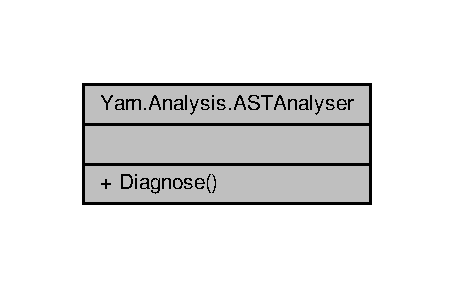
\includegraphics[width=218pt]{db/d77/a00683}
\end{center}
\end{figure}
\subsection*{Public Member Functions}
\begin{DoxyCompactItemize}
\item 
abstract I\-Enumerable$<$ \hyperlink{a00071}{Diagnosis} $>$ \hyperlink{a00021_a07bb220dead44ed12c8842de706ecdf7}{Diagnose} (\hyperlink{a00112}{Yarn.\-Parser.\-Node} node)
\end{DoxyCompactItemize}


\subsection{Detailed Description}


\subsection{Member Function Documentation}
\hypertarget{a00021_a07bb220dead44ed12c8842de706ecdf7}{\index{Yarn\-::\-Analysis\-::\-A\-S\-T\-Analyser@{Yarn\-::\-Analysis\-::\-A\-S\-T\-Analyser}!Diagnose@{Diagnose}}
\index{Diagnose@{Diagnose}!Yarn::Analysis::ASTAnalyser@{Yarn\-::\-Analysis\-::\-A\-S\-T\-Analyser}}
\subsubsection[{Diagnose}]{\setlength{\rightskip}{0pt plus 5cm}abstract I\-Enumerable$<${\bf Diagnosis}$>$ Yarn.\-Analysis.\-A\-S\-T\-Analyser.\-Diagnose (
\begin{DoxyParamCaption}
\item[{{\bf Yarn.\-Parser.\-Node}}]{node}
\end{DoxyParamCaption}
)\hspace{0.3cm}{\ttfamily [pure virtual]}}}\label{a00021_a07bb220dead44ed12c8842de706ecdf7}


The documentation for this class was generated from the following file\-:\begin{DoxyCompactItemize}
\item 
Yarn\-Spinner/\hyperlink{a00263}{Analyser.\-cs}\end{DoxyCompactItemize}

\subsection*{Style Guide}

{\ttfamily Inline Code} contain short snippets of code for your project \begin{DoxyVerb}Code Blocks contain segments or chunks of code for your project
\end{DoxyVerb}


{\bfseries Bold indicate actions (Select menu item, copying file, etc.)}

$\ast$$\ast$$\ast$\-Bold italic text indicates emphasis$\ast$$\ast$$\ast$

\begin{quotation}
Blockquotes contain essential information

\end{quotation}


\subsection*{Introduction}

This document intends to demonstrate to a developer how they can add new functions so that they can be called from inside \hyperlink{a00048}{Yarn}.

\subsubsection*{Programming style}


\begin{DoxyItemize}
\item It is recommended that you follow our programming style so that in the case of bug or patch submission, it makes it easier for us to read. As such, indents should be four spaces and not tab stops.
\item We use the Doxygen format for documentation, thus three forward slashes {\ttfamily ///} indicate the head of a documentation comment and details for documentation comments are contained within the {\ttfamily /$\ast$ ....} structure. Please refer to the Doxygen site for more information.
\item Other comments should use two forward slashes. This will ensure proper code commentary without it appearing in generated A\-P\-I documentation.
\end{DoxyItemize}

\subsection*{Creating a custom command}

Creating a custom command is a simple two step procedure.\-i


\begin{DoxyEnumerate}
\item We need to get the dialogue object that's in use, then regiser a new function for it. ``` // get the Dialogue object // varstorage\-\_\-implementation is the object that handles variable storage -\/ it's not important in this example var dialogue = new Dialogue(varstorage\-\_\-implementation); ``{\ttfamily }
\item {\ttfamily Next, register your new function. For example, let's make a function that takes 1 parameter, which is a number, and returns}true{\ttfamily if it's even\-: }`` // Register\-Function(name, parameter\-Count, implementation) dialogue.\-library.\-Register\-Function (\char`\"{}is\-\_\-even\char`\"{}, 1, delegate(\-Value\mbox{[}$\,$\mbox{]} parameters) \{ return (int)parameters\mbox{[}0\mbox{]}.As\-Number \% 2 == 0; \}); ``` When the function is called, the delegate you provide will be run.
\end{DoxyEnumerate}

Some notes\-:


\begin{DoxyItemize}
\item You don't have to return a value from your function.
\item The parameters passed to your function are of type \hyperlink{a00165}{Yarn.\-Value}. You can get their value as numbers, bools or strings by using the {\ttfamily As\-Number}, {\ttfamily As\-String} and {\ttfamily As\-Bool} properties.
\item You can only return values of the following types\-:
\begin{DoxyItemize}
\item String
\item Float
\item Double
\item Integer
\item \hyperlink{a00165}{Yarn.\-Value}
\end{DoxyItemize}
\item \hyperlink{a00048}{Yarn} Spinner will make sure that the correct number of parameters is passed to your method. If you specify {\ttfamily -\/1} as your parameter count, the function may have any number of parameters. 
\end{DoxyItemize}
\hypertarget{a00023}{\section{Yarn.\-Unity.\-Example.\-Camera\-Follow Class Reference}
\label{a00023}\index{Yarn.\-Unity.\-Example.\-Camera\-Follow@{Yarn.\-Unity.\-Example.\-Camera\-Follow}}
}


Inheritance diagram for Yarn.\-Unity.\-Example.\-Camera\-Follow\-:
\nopagebreak
\begin{figure}[H]
\begin{center}
\leavevmode
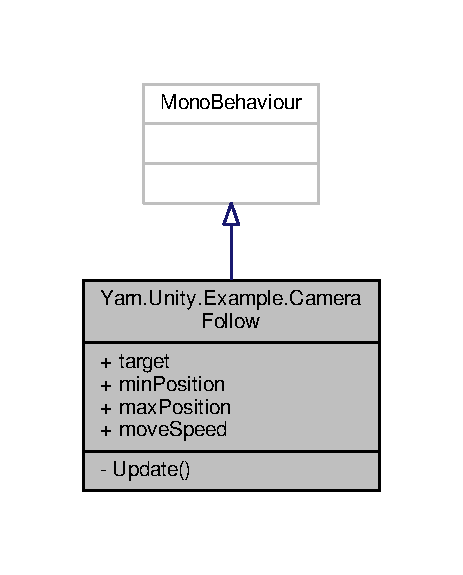
\includegraphics[width=222pt]{a00348}
\end{center}
\end{figure}


Collaboration diagram for Yarn.\-Unity.\-Example.\-Camera\-Follow\-:
\nopagebreak
\begin{figure}[H]
\begin{center}
\leavevmode
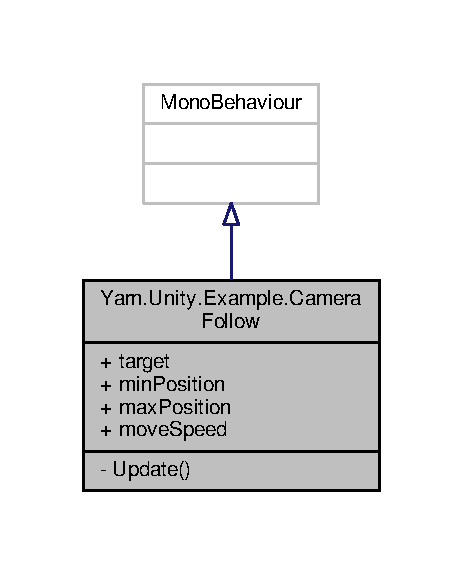
\includegraphics[width=222pt]{a00349}
\end{center}
\end{figure}
\subsection*{Public Attributes}
\begin{DoxyCompactItemize}
\item 
Transform \hyperlink{a00023_aa5d6958fb14a14ebb74e21c372fcca8b}{target}
\item 
float \hyperlink{a00023_a08c6f6c0ea423c21af99e4b5467d3c9b}{min\-Position} = -\/5.\-3f
\item 
float \hyperlink{a00023_abb0154dcbc2a7d43795beacd61a56de4}{max\-Position} = 5.\-3f
\item 
float \hyperlink{a00023_a3d4f2efe9c2cee8c7ff797cac03f27ec}{move\-Speed} = 1.\-0f
\end{DoxyCompactItemize}
\subsection*{Private Member Functions}
\begin{DoxyCompactItemize}
\item 
void \hyperlink{a00023_a592ddbf8e493bde0a6536c0234869217}{Update} ()
\end{DoxyCompactItemize}


\subsection{Detailed Description}


\subsection{Member Function Documentation}
\hypertarget{a00023_a592ddbf8e493bde0a6536c0234869217}{\index{Yarn\-::\-Unity\-::\-Example\-::\-Camera\-Follow@{Yarn\-::\-Unity\-::\-Example\-::\-Camera\-Follow}!Update@{Update}}
\index{Update@{Update}!Yarn::Unity::Example::CameraFollow@{Yarn\-::\-Unity\-::\-Example\-::\-Camera\-Follow}}
\subsubsection[{Update}]{\setlength{\rightskip}{0pt plus 5cm}void Yarn.\-Unity.\-Example.\-Camera\-Follow.\-Update (
\begin{DoxyParamCaption}
{}
\end{DoxyParamCaption}
)\hspace{0.3cm}{\ttfamily [private]}}}\label{a00023_a592ddbf8e493bde0a6536c0234869217}

\begin{DoxyCode}
42                        \{
43             \textcolor{keywordflow}{if} (\hyperlink{a00023_aa5d6958fb14a14ebb74e21c372fcca8b}{target} == null) \{
44                 \textcolor{keywordflow}{return};
45             \}
46             var newPosition = Vector3.Lerp(transform.position, target.position, 
      \hyperlink{a00023_a3d4f2efe9c2cee8c7ff797cac03f27ec}{moveSpeed} * Time.deltaTime);
47 
48             newPosition.x = Mathf.Clamp(newPosition.x, \hyperlink{a00023_a08c6f6c0ea423c21af99e4b5467d3c9b}{minPosition}, 
      \hyperlink{a00023_abb0154dcbc2a7d43795beacd61a56de4}{maxPosition});
49             newPosition.y = transform.position.y;
50             newPosition.z = transform.position.z;
51 
52             transform.position = newPosition;
53         \}
\end{DoxyCode}


\subsection{Member Data Documentation}
\hypertarget{a00023_abb0154dcbc2a7d43795beacd61a56de4}{\index{Yarn\-::\-Unity\-::\-Example\-::\-Camera\-Follow@{Yarn\-::\-Unity\-::\-Example\-::\-Camera\-Follow}!max\-Position@{max\-Position}}
\index{max\-Position@{max\-Position}!Yarn::Unity::Example::CameraFollow@{Yarn\-::\-Unity\-::\-Example\-::\-Camera\-Follow}}
\subsubsection[{max\-Position}]{\setlength{\rightskip}{0pt plus 5cm}float Yarn.\-Unity.\-Example.\-Camera\-Follow.\-max\-Position = 5.\-3f}}\label{a00023_abb0154dcbc2a7d43795beacd61a56de4}
\hypertarget{a00023_a08c6f6c0ea423c21af99e4b5467d3c9b}{\index{Yarn\-::\-Unity\-::\-Example\-::\-Camera\-Follow@{Yarn\-::\-Unity\-::\-Example\-::\-Camera\-Follow}!min\-Position@{min\-Position}}
\index{min\-Position@{min\-Position}!Yarn::Unity::Example::CameraFollow@{Yarn\-::\-Unity\-::\-Example\-::\-Camera\-Follow}}
\subsubsection[{min\-Position}]{\setlength{\rightskip}{0pt plus 5cm}float Yarn.\-Unity.\-Example.\-Camera\-Follow.\-min\-Position = -\/5.\-3f}}\label{a00023_a08c6f6c0ea423c21af99e4b5467d3c9b}
\hypertarget{a00023_a3d4f2efe9c2cee8c7ff797cac03f27ec}{\index{Yarn\-::\-Unity\-::\-Example\-::\-Camera\-Follow@{Yarn\-::\-Unity\-::\-Example\-::\-Camera\-Follow}!move\-Speed@{move\-Speed}}
\index{move\-Speed@{move\-Speed}!Yarn::Unity::Example::CameraFollow@{Yarn\-::\-Unity\-::\-Example\-::\-Camera\-Follow}}
\subsubsection[{move\-Speed}]{\setlength{\rightskip}{0pt plus 5cm}float Yarn.\-Unity.\-Example.\-Camera\-Follow.\-move\-Speed = 1.\-0f}}\label{a00023_a3d4f2efe9c2cee8c7ff797cac03f27ec}
\hypertarget{a00023_aa5d6958fb14a14ebb74e21c372fcca8b}{\index{Yarn\-::\-Unity\-::\-Example\-::\-Camera\-Follow@{Yarn\-::\-Unity\-::\-Example\-::\-Camera\-Follow}!target@{target}}
\index{target@{target}!Yarn::Unity::Example::CameraFollow@{Yarn\-::\-Unity\-::\-Example\-::\-Camera\-Follow}}
\subsubsection[{target}]{\setlength{\rightskip}{0pt plus 5cm}Transform Yarn.\-Unity.\-Example.\-Camera\-Follow.\-target}}\label{a00023_aa5d6958fb14a14ebb74e21c372fcca8b}


The documentation for this class was generated from the following file\-:\begin{DoxyCompactItemize}
\item 
Unity/\-Assets/\-Yarn Spinner/\-Examples/\-Demo Scripts/\hyperlink{a00108}{Camera\-Follow.\-cs}\end{DoxyCompactItemize}

\subsubsection*{Style Guide}

{\ttfamily Inline Code} contain short snippets of code for your project \begin{DoxyVerb}Code Blocks contain segments or chunks of code for your project
\end{DoxyVerb}


{\bfseries Bold indicate actions (Select menu item, copying file, etc.)}

$\ast$$\ast$$\ast$\-Bold italic text indicates emphasis$\ast$$\ast$$\ast$

\begin{quotation}
Blockquotes contain essential information

\end{quotation}


\subsection*{Tutorial}

\begin{quotation}
$\ast$$\ast$$\ast$\-Note\-:$\ast$$\ast$$\ast$ This tutorial assumes that you know a little bit about \href{http://www.unity3d.com}{\tt Unity}. In particular, it is helpful that you know how to get around the Unity editor, how to work with game objects, and how to write scripts in C\#. If you don't know these things, please refer to \href{http://unity3d.com/learn}{\tt Unity's documentation}.

\end{quotation}


\subsection*{Step by Step}

\subsubsection*{Introducing \hyperlink{a00051}{Yarn} Spinner}

\hyperlink{a00051}{Yarn} Spinner is designed to be easy to work with in Unity. It makes no assumptions about how your game presents dialogue to the player, or about how the player chooses their responses.

To introduce \hyperlink{a00051}{Yarn} Spinner, we'll create an empty Unity project, and then build it from the ground up to run a sample conversation. If you'd first like to see the finished project, \href{https://github.com/thesecretlab/YarnSpinner/releases}{\tt download Yarn Spinner} and open the \href{https://github.com/thesecretlab/YarnSpinner/tree/master/Unity}{\tt Unity folder} in the Unity editor. To build a standalone version of this loaded project, skip to the end of this documentation.

To use \hyperlink{a00051}{Yarn} Spinner, you use three classes that will exist in the {\ttfamily \hyperlink{a00135}{Yarn.\-Unity}} namespace.


\begin{DoxyItemize}
\item {\ttfamily Dialogue\-Runner}, which is responsible for loading and running your dialogue script;
\item A subclass of {\ttfamily Dialogue\-U\-I\-Behaviour}, which is reponsible for displaying the lines and dialogue choices to the player; and
\item A subclass of {\ttfamily Variable\-Storage\-Behaviour}, which is responsible for storing the state of the conversation.
\end{DoxyItemize}

To create your subclasses of {\ttfamily Dialogue\-U\-I\-Behaviour} and {\ttfamily Variable\-Storage\-Behaviour}, you'll need to add the following code to the top of your C\# code\-: \begin{DoxyVerb}using Yarn.Unity;
\end{DoxyVerb}


\hyperlink{a00051}{Yarn} dialogue is created using the \href{http://github.com/infiniteammoinc/Yarn}{\tt Yarn Editor}, and the resulting dialogue is stored as {\ttfamily .json} assets in the Unity project. If you are using Linux and wish to use the \hyperlink{a00051}{Yarn} Editor, you will first need to \href{https://nwjs.io/downloads/}{\tt install} or build \href{https://nwjs.io/}{\tt N\-W.\-js} then attempt to build the \hyperlink{a00051}{Yarn} Editor. {\bfseries N\-O\-T\-E A\-T T\-H\-I\-S S\-T\-A\-G\-E, B\-U\-I\-L\-D\-I\-N\-G N\-W.\-J\-S H\-A\-S N\-O\-T B\-E\-E\-N A\-T\-T\-E\-M\-P\-T\-E\-D B\-Y U\-S A\-N\-D M\-A\-Y S\-E\-T Y\-O\-U\-R C\-O\-M\-P\-U\-T\-E\-R O\-N F\-I\-R\-E}.

The \hyperlink{a00051}{Yarn} dialogue files can be stored anywhere inside the project hierarchy -\/ you simply provide add them to the {\ttfamily Dialogue\-Runner}'s inspector. You can also call {\ttfamily Add\-Script} on the {\ttfamily Dialogue\-Runner} at runtime; this is useful for cases such as spawning a character who comes with additional dialogue -\/ all that needs to happen is the character then pass their \hyperlink{a00051}{Yarn} script to the {\ttfamily Dialogue\-Runner}.

\subsubsection*{Create the \hyperlink{a00051}{Yarn} conversations}


\begin{DoxyItemize}
\item In the \hyperlink{a00051}{Yarn} Editor, {\bfseries Create a new conversation}, and save it as a J\-S\-O\-N file. (Alternatively, if you already have a dialogue file you'd like to use, go ahead and use that instead!). For information on how to create a \hyperlink{a00051}{Yarn} conversation, please refer to the \hyperlink{a00051}{Yarn} Editor site.
\end{DoxyItemize}

\subsubsection*{Create the Unity project}


\begin{DoxyItemize}
\item {\bfseries Launch Unity}, and {\bfseries create a new project}. The name of the project doesn't matter.
\end{DoxyItemize}

\subsubsection*{Import the \hyperlink{a00051}{Yarn} Spinner package.}


\begin{DoxyItemize}
\item $\ast$$\ast$\href{https://github.com/thesecretlab/YarnSpinner/releases}{\tt Import Yarn\-Spinner.\-unitypackage}$\ast$$\ast$ into your project.

\hyperlink{a00051}{Yarn} Spinner is composed of a {\ttfamily yarnspinner.\-dll} file, and a couple of supporting scripts for Unity. This dll file does the heavy lifting involved in parsing your \hyperlink{a00051}{Yarn} files, and executing them.

To show \hyperlink{a00051}{Yarn} dialogue in your game, you will need to add it to your project as well.
\item {\bfseries Copy your \hyperlink{a00051}{Yarn} J\-S\-O\-N file} into your project.
\end{DoxyItemize}

You're now ready to start using \hyperlink{a00051}{Yarn} Spinner!

\subsubsection*{Load your conversation with {\ttfamily Dialogue\-Runner}}

\hyperlink{a00051}{Yarn} conversations are loaded and managed by a {\ttfamily Dialogue\-Runner} object. This object is responsible for loading and parsing your \hyperlink{a00051}{Yarn} {\ttfamily .json} files. It also runs the script when it's told to -\/ for example, when you walk up to a character in your game and talk to them.

We'll start by creating an empty object, and then we'll add the {\ttfamily Dialogue\-Runner} component to it.


\begin{DoxyItemize}
\item {\bfseries Create a new empty game object}.
\item {\bfseries Rename it to \char`\"{}\-Dialogue Runner\char`\"{}}.
\item With the Dialogue Runner object selected, {\bfseries open the Component menu}, and choose {\bfseries Scripts → \hyperlink{a00051}{Yarn} Spinner → Dialogue Runner}.

Next you need to add the \hyperlink{a00051}{Yarn} files that you want to show. The Dialogue runner can load multiple \hyperlink{a00051}{Yarn} files at the same time. The only requirement is that {\bfseries no nodes are allowed to have the same name}. (This is a requirement that may change in the future.)
\item {\bfseries Drag your \hyperlink{a00051}{Yarn} J\-S\-O\-N file into the {\ttfamily Source Text} array.}
\end{DoxyItemize}

\subsubsection*{Display your conversation with {\ttfamily Dialogue\-U\-I}}

Your game's dialogue needs to be shown to the user. Additionally, you need a way to let the player choose what their reaction is going to be.

\hyperlink{a00051}{Yarn} Spinner makes no assumptions about how you want to handle your dialogue's U\-I. Want to present as simple list of options? That's fine. Want a fancy Mass Effect style radial menu? Totally cool. Want a totally bonkers gesture-\/based U\-I with a countdown timer? Oh man that would be sweet.

\hyperlink{a00051}{Yarn} Spinner leaves all of the work of actually presenting the conversation up to you; all it's responsible for is delivering the lines that the player should see, and notifying \hyperlink{a00051}{Yarn} Spinner about what response the user selected.

\hyperlink{a00051}{Yarn} Spinner comes with an example script that uses Unity's U\-I system. It's a good place to start.

\subsubsection*{Store your conversation state with a {\ttfamily Variable\-Storage\-Behaviour}}

There's one last necessary component. As you play through a conversation, you'll probably want to record the user's choices somewhere. \hyperlink{a00051}{Yarn} Spinner doesn't care about the details of how you save your game state; instead, it just expects you to give it an object that conforms to a $\ast$$\ast$$\ast$\href{https://docs.microsoft.com/en-us/dotnet/csharp/programming-guide/interfaces/index}{\tt C\# interface})$\ast$$\ast$$\ast$, which defines methods like \char`\"{}set variable\char`\"{} and \char`\"{}get value of variable\char`\"{}.

The simplest implementation of this is one that just keeps your variables in memory, but it's pretty straightforward to adapt an existing save game system to use it.


\begin{DoxyItemize}
\item {\bfseries Create a new game object}, and add the {\ttfamily \hyperlink{a00089}{Example\-Variable\-Storage}} script to it.
\end{DoxyItemize}

Or\-:


\begin{DoxyItemize}
\item {\bfseries Create a new game object}, and add a new script to it. Make this script subclass {\ttfamily Variable\-Storage\-Behaviour}, and the implement the {\ttfamily Set\-Number}, {\ttfamily Get\-Number}, {\ttfamily Clear}, and {\ttfamily Reset\-To\-Defaults} methods.
\item Once you've done that, {\bfseries drag this new object into the Dialoge Runner's {\ttfamily Variable Storage} slot.}
\end{DoxyItemize}

\subsubsection*{Run your conversation}

There's only one thing left to do\-: \hyperlink{a00051}{Yarn} Spinner just needs to know what node in the \hyperlink{a00051}{Yarn} file to start from. It will default to \char`\"{}\-Start\char`\"{}, but you can override it.


\begin{DoxyItemize}
\item {\bfseries Change the Dialogue Runner's {\ttfamily Start Node}} to the {\bfseries name of the node you'd like to start run.}
\item Finally, {\bfseries run the game.} The conversation will play!
\end{DoxyItemize}

\subsubsection*{Respond to commands with {\ttfamily Yarn\-Command}}

In \hyperlink{a00051}{Yarn}, you can create {\itshape commands} that tell your game to do something. For example, if you want a character to move to a certain point on the screen, you might have a command that looks like this\-: \begin{DoxyVerb}<<move Sally exit>>
\end{DoxyVerb}


For this to work, the game object named \char`\"{}\-Sally\char`\"{} needs to have a script component attached to it, and one of those scripts needs to have a method that looks like this\-: \begin{DoxyVerb}[YarnCommand("move")]
public void MoveCharacter(string destinationName) {
    // move to the destination
}
\end{DoxyVerb}


When \hyperlink{a00051}{Yarn} encounters a command that contains two or more words, it looks for a game object with the same name as the second word (\char`\"{}\-Sally\char`\"{}, in the above example), and then searches that object's scripts for any method that has a {\ttfamily Yarn\-Command} with the same name as the first word (in this case, \char`\"{}move\char`\"{}).

Any further words in the command are passed as string parameters to the method (\char`\"{}exit\char`\"{}, in this case, which is used as the {\ttfamily destination\-Name} parameter)

Note that {\bfseries all} parameters must be strings. {\ttfamily Dialogue\-Runner} will throw an error if it finds a method that has parameters of any other type. It's up to your method to convert the strings into other types, like numbers.

\subsubsection*{Finishing up}

Save the project

Build a stand alone 
\hypertarget{a00025}{\section{Yarn.\-Parser.\-If\-Statement.\-Clause Struct Reference}
\label{a00025}\index{Yarn.\-Parser.\-If\-Statement.\-Clause@{Yarn.\-Parser.\-If\-Statement.\-Clause}}
}


Collaboration diagram for Yarn.\-Parser.\-If\-Statement.\-Clause\-:
\nopagebreak
\begin{figure}[H]
\begin{center}
\leavevmode
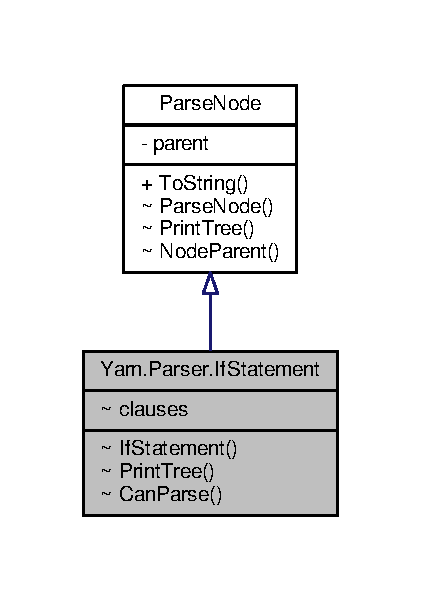
\includegraphics[height=550pt]{d9/d2a/a00270}
\end{center}
\end{figure}
\subsection*{Package Functions}
\begin{DoxyCompactItemize}
\item 
string \hyperlink{a00025_a7f4fc9399896512b68fdc7bc7cf818c9}{Print\-Tree} (int indent\-Level)
\end{DoxyCompactItemize}
\subsection*{Package Attributes}
\begin{DoxyCompactItemize}
\item 
\hyperlink{a00040}{Expression} \hyperlink{a00025_a1abd1f7c41f68ccdf64074ea49365be9}{expression}
\item 
I\-Enumerable$<$ \hyperlink{a00076}{Statement} $>$ \hyperlink{a00025_a6f4765482e98ed042e38a0ede13f171f}{statements}
\end{DoxyCompactItemize}


\subsection{Detailed Description}


\subsection{Member Function Documentation}
\hypertarget{a00025_a7f4fc9399896512b68fdc7bc7cf818c9}{\index{Yarn\-::\-Parser\-::\-If\-Statement\-::\-Clause@{Yarn\-::\-Parser\-::\-If\-Statement\-::\-Clause}!Print\-Tree@{Print\-Tree}}
\index{Print\-Tree@{Print\-Tree}!Yarn::Parser::IfStatement::Clause@{Yarn\-::\-Parser\-::\-If\-Statement\-::\-Clause}}
\subsubsection[{Print\-Tree}]{\setlength{\rightskip}{0pt plus 5cm}string Yarn.\-Parser.\-If\-Statement.\-Clause.\-Print\-Tree (
\begin{DoxyParamCaption}
\item[{int}]{indent\-Level}
\end{DoxyParamCaption}
)\hspace{0.3cm}{\ttfamily [package]}}}\label{a00025_a7f4fc9399896512b68fdc7bc7cf818c9}

\begin{DoxyCode}
536                                                            \{
537                     var sb = \textcolor{keyword}{new} StringBuilder ();
538                     \textcolor{keywordflow}{if} (\hyperlink{a00025_a1abd1f7c41f68ccdf64074ea49365be9}{expression} != null)
539                         sb.Append (expression.PrintTree (indentLevel));
540                     sb.Append (\hyperlink{a00064_aa8fa36b46de12a1c561d77b99c4b9ae3}{Tab} (indentLevel, \textcolor{stringliteral}{"\{"}));
541                     \textcolor{keywordflow}{foreach} (var statement \textcolor{keywordflow}{in} \hyperlink{a00025_a6f4765482e98ed042e38a0ede13f171f}{statements}) \{
542                         sb.Append (statement.PrintTree (indentLevel + 1));
543                     \}
544                     sb.Append (\hyperlink{a00064_aa8fa36b46de12a1c561d77b99c4b9ae3}{Tab} (indentLevel, \textcolor{stringliteral}{"\}"}));
545                     \textcolor{keywordflow}{return} sb.ToString ();
546                 \}
\end{DoxyCode}


\subsection{Member Data Documentation}
\hypertarget{a00025_a1abd1f7c41f68ccdf64074ea49365be9}{\index{Yarn\-::\-Parser\-::\-If\-Statement\-::\-Clause@{Yarn\-::\-Parser\-::\-If\-Statement\-::\-Clause}!expression@{expression}}
\index{expression@{expression}!Yarn::Parser::IfStatement::Clause@{Yarn\-::\-Parser\-::\-If\-Statement\-::\-Clause}}
\subsubsection[{expression}]{\setlength{\rightskip}{0pt plus 5cm}{\bf Expression} Yarn.\-Parser.\-If\-Statement.\-Clause.\-expression\hspace{0.3cm}{\ttfamily [package]}}}\label{a00025_a1abd1f7c41f68ccdf64074ea49365be9}
\hypertarget{a00025_a6f4765482e98ed042e38a0ede13f171f}{\index{Yarn\-::\-Parser\-::\-If\-Statement\-::\-Clause@{Yarn\-::\-Parser\-::\-If\-Statement\-::\-Clause}!statements@{statements}}
\index{statements@{statements}!Yarn::Parser::IfStatement::Clause@{Yarn\-::\-Parser\-::\-If\-Statement\-::\-Clause}}
\subsubsection[{statements}]{\setlength{\rightskip}{0pt plus 5cm}I\-Enumerable$<${\bf Statement}$>$ Yarn.\-Parser.\-If\-Statement.\-Clause.\-statements\hspace{0.3cm}{\ttfamily [package]}}}\label{a00025_a6f4765482e98ed042e38a0ede13f171f}


The documentation for this struct was generated from the following file\-:\begin{DoxyCompactItemize}
\item 
Yarn\-Spinner/\hyperlink{a00122}{Parser.\-cs}\end{DoxyCompactItemize}

\hypertarget{a00027}{\section{Yarn.\-Add\-Labels\-Options Class Reference}
\label{a00027}\index{Yarn.\-Add\-Labels\-Options@{Yarn.\-Add\-Labels\-Options}}
}


Inheritance diagram for Yarn.\-Add\-Labels\-Options\-:
\nopagebreak
\begin{figure}[H]
\begin{center}
\leavevmode
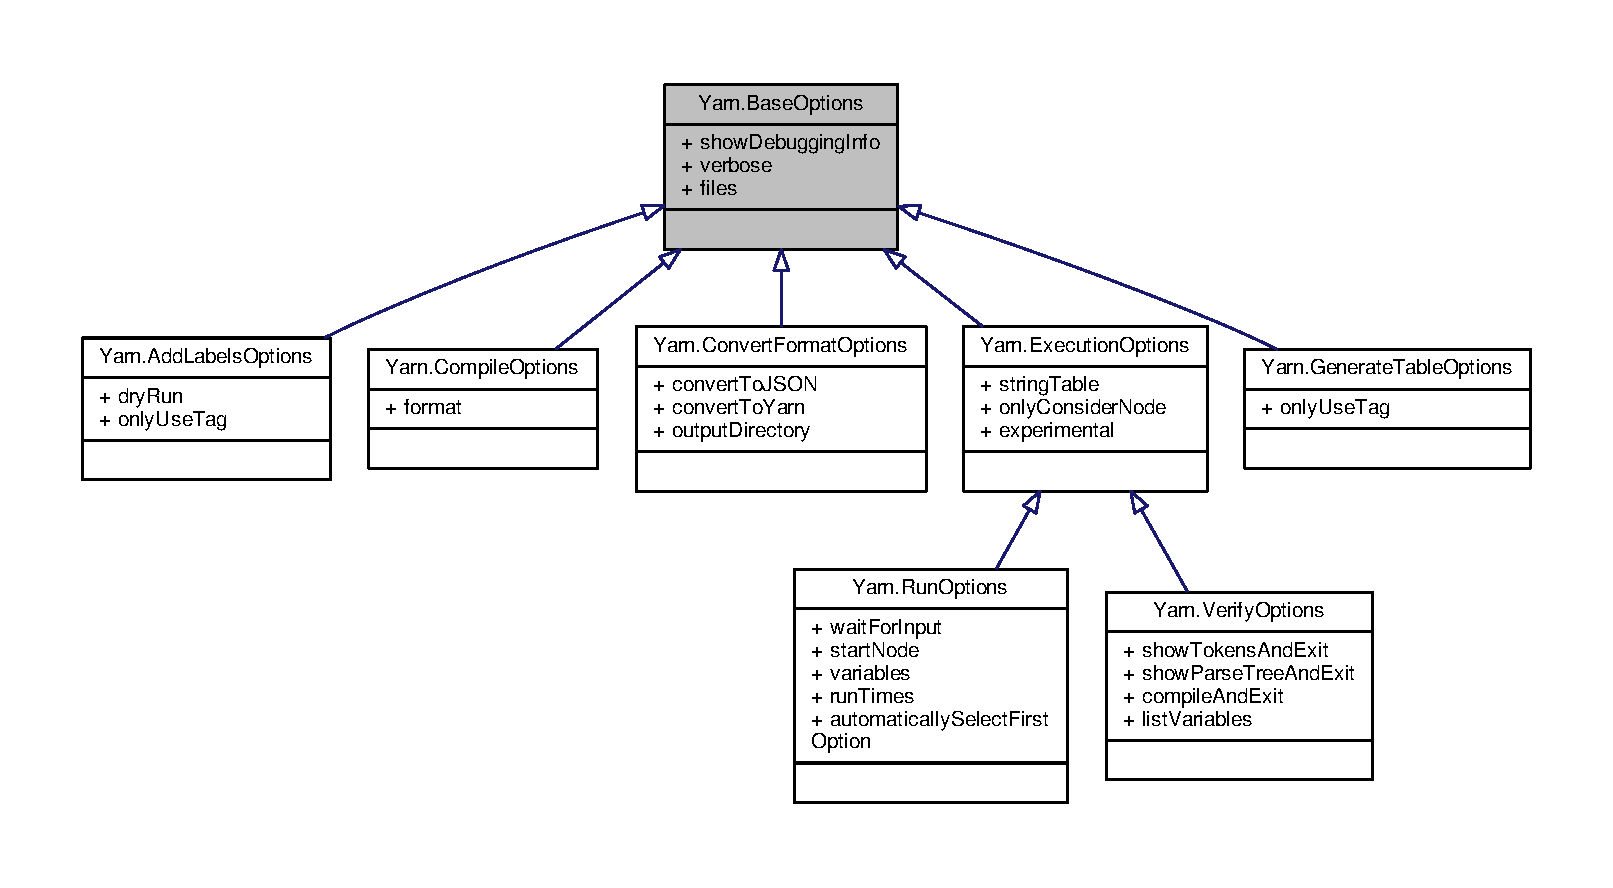
\includegraphics[width=198pt]{a00732}
\end{center}
\end{figure}


Collaboration diagram for Yarn.\-Add\-Labels\-Options\-:
\nopagebreak
\begin{figure}[H]
\begin{center}
\leavevmode
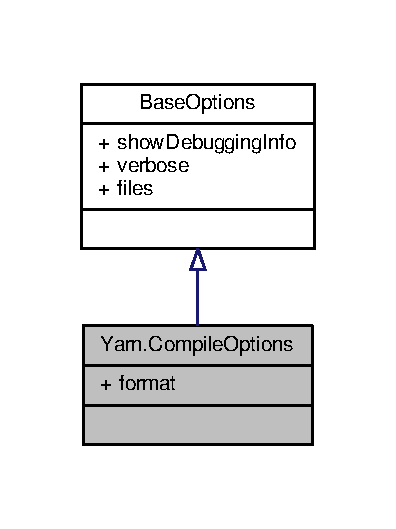
\includegraphics[width=198pt]{a00733}
\end{center}
\end{figure}
\subsection*{Properties}
\begin{DoxyCompactItemize}
\item 
bool \hyperlink{a00027_a5dc9d9db767738237e988f95fc0330f4}{dry\-Run}\hspace{0.3cm}{\ttfamily  \mbox{[}get, set\mbox{]}}
\item 
string \hyperlink{a00027_ab6162338f9606a836f3101fe0e228249}{only\-Use\-Tag}\hspace{0.3cm}{\ttfamily  \mbox{[}get, set\mbox{]}}
\item 
bool \hyperlink{a00031_a89964ea17bd19caf00cb5bff563ed01c}{show\-Debugging\-Info}\hspace{0.3cm}{\ttfamily  \mbox{[}get, set\mbox{]}}
\item 
bool \hyperlink{a00031_ada4d83d1756918f362d55f6649b82b17}{verbose}\hspace{0.3cm}{\ttfamily  \mbox{[}get, set\mbox{]}}
\item 
I\-List$<$ string $>$ \hyperlink{a00031_aa93cbb1bc1d5328e0a417012621e92d2}{files}\hspace{0.3cm}{\ttfamily  \mbox{[}get, set\mbox{]}}
\end{DoxyCompactItemize}


\subsection{Detailed Description}


Definition at line 116 of file Main.\-cs.



\subsection{Property Documentation}
\hypertarget{a00027_a5dc9d9db767738237e988f95fc0330f4}{\index{Yarn\-::\-Add\-Labels\-Options@{Yarn\-::\-Add\-Labels\-Options}!dry\-Run@{dry\-Run}}
\index{dry\-Run@{dry\-Run}!Yarn::AddLabelsOptions@{Yarn\-::\-Add\-Labels\-Options}}
\subsubsection[{dry\-Run}]{\setlength{\rightskip}{0pt plus 5cm}bool Yarn.\-Add\-Labels\-Options.\-dry\-Run\hspace{0.3cm}{\ttfamily [get]}, {\ttfamily [set]}}}\label{a00027_a5dc9d9db767738237e988f95fc0330f4}


Definition at line 120 of file Main.\-cs.

\hypertarget{a00031_aa93cbb1bc1d5328e0a417012621e92d2}{\index{Yarn\-::\-Add\-Labels\-Options@{Yarn\-::\-Add\-Labels\-Options}!files@{files}}
\index{files@{files}!Yarn::AddLabelsOptions@{Yarn\-::\-Add\-Labels\-Options}}
\subsubsection[{files}]{\setlength{\rightskip}{0pt plus 5cm}I\-List$<$string$>$ Yarn.\-Base\-Options.\-files\hspace{0.3cm}{\ttfamily [get]}, {\ttfamily [set]}, {\ttfamily [inherited]}}}\label{a00031_aa93cbb1bc1d5328e0a417012621e92d2}


Definition at line 47 of file Main.\-cs.



Referenced by Yarn.\-Yarn\-Spinner\-Console.\-Run(), and Yarn.\-Yarn\-Spinner\-Console.\-Verify().

\hypertarget{a00027_ab6162338f9606a836f3101fe0e228249}{\index{Yarn\-::\-Add\-Labels\-Options@{Yarn\-::\-Add\-Labels\-Options}!only\-Use\-Tag@{only\-Use\-Tag}}
\index{only\-Use\-Tag@{only\-Use\-Tag}!Yarn::AddLabelsOptions@{Yarn\-::\-Add\-Labels\-Options}}
\subsubsection[{only\-Use\-Tag}]{\setlength{\rightskip}{0pt plus 5cm}string Yarn.\-Add\-Labels\-Options.\-only\-Use\-Tag\hspace{0.3cm}{\ttfamily [get]}, {\ttfamily [set]}}}\label{a00027_ab6162338f9606a836f3101fe0e228249}


Definition at line 123 of file Main.\-cs.

\hypertarget{a00031_a89964ea17bd19caf00cb5bff563ed01c}{\index{Yarn\-::\-Add\-Labels\-Options@{Yarn\-::\-Add\-Labels\-Options}!show\-Debugging\-Info@{show\-Debugging\-Info}}
\index{show\-Debugging\-Info@{show\-Debugging\-Info}!Yarn::AddLabelsOptions@{Yarn\-::\-Add\-Labels\-Options}}
\subsubsection[{show\-Debugging\-Info}]{\setlength{\rightskip}{0pt plus 5cm}bool Yarn.\-Base\-Options.\-show\-Debugging\-Info\hspace{0.3cm}{\ttfamily [get]}, {\ttfamily [set]}, {\ttfamily [inherited]}}}\label{a00031_a89964ea17bd19caf00cb5bff563ed01c}


Definition at line 40 of file Main.\-cs.



Referenced by Yarn.\-Yarn\-Spinner\-Console.\-Create\-Dialogue().

\hypertarget{a00031_ada4d83d1756918f362d55f6649b82b17}{\index{Yarn\-::\-Add\-Labels\-Options@{Yarn\-::\-Add\-Labels\-Options}!verbose@{verbose}}
\index{verbose@{verbose}!Yarn::AddLabelsOptions@{Yarn\-::\-Add\-Labels\-Options}}
\subsubsection[{verbose}]{\setlength{\rightskip}{0pt plus 5cm}bool Yarn.\-Base\-Options.\-verbose\hspace{0.3cm}{\ttfamily [get]}, {\ttfamily [set]}, {\ttfamily [inherited]}}}\label{a00031_ada4d83d1756918f362d55f6649b82b17}


Definition at line 44 of file Main.\-cs.



Referenced by Yarn.\-File\-Format\-Converter.\-Convert\-Nodes\-In\-File(), and Yarn.\-Table\-Generator.\-Generate\-Tables().



The documentation for this class was generated from the following file\-:\begin{DoxyCompactItemize}
\item 
Yarn\-Spinner\-Console/\hyperlink{a00307}{Main.\-cs}\end{DoxyCompactItemize}

\hypertarget{a00028}{\section{Yarn.\-Parser.\-If\-Statement.\-Clause Struct Reference}
\label{a00028}\index{Yarn.\-Parser.\-If\-Statement.\-Clause@{Yarn.\-Parser.\-If\-Statement.\-Clause}}
}


Collaboration diagram for Yarn.\-Parser.\-If\-Statement.\-Clause\-:
\nopagebreak
\begin{figure}[H]
\begin{center}
\leavevmode
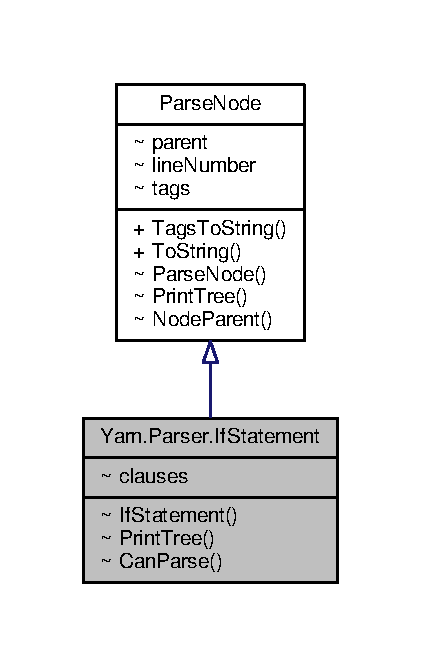
\includegraphics[height=550pt]{d6/d75/a00604}
\end{center}
\end{figure}
\subsection*{Package Functions}
\begin{DoxyCompactItemize}
\item 
string \hyperlink{a00028_a7f4fc9399896512b68fdc7bc7cf818c9}{Print\-Tree} (int indent\-Level)
\end{DoxyCompactItemize}
\subsection*{Package Attributes}
\begin{DoxyCompactItemize}
\item 
\hyperlink{a00080}{Expression} \hyperlink{a00028_a1abd1f7c41f68ccdf64074ea49365be9}{expression}
\item 
I\-Enumerable$<$ \hyperlink{a00140}{Statement} $>$ \hyperlink{a00028_a6f4765482e98ed042e38a0ede13f171f}{statements}
\end{DoxyCompactItemize}


\subsection{Detailed Description}


\subsection{Member Function Documentation}
\hypertarget{a00028_a7f4fc9399896512b68fdc7bc7cf818c9}{\index{Yarn\-::\-Parser\-::\-If\-Statement\-::\-Clause@{Yarn\-::\-Parser\-::\-If\-Statement\-::\-Clause}!Print\-Tree@{Print\-Tree}}
\index{Print\-Tree@{Print\-Tree}!Yarn::Parser::IfStatement::Clause@{Yarn\-::\-Parser\-::\-If\-Statement\-::\-Clause}}
\subsubsection[{Print\-Tree}]{\setlength{\rightskip}{0pt plus 5cm}string Yarn.\-Parser.\-If\-Statement.\-Clause.\-Print\-Tree (
\begin{DoxyParamCaption}
\item[{int}]{indent\-Level}
\end{DoxyParamCaption}
)\hspace{0.3cm}{\ttfamily [package]}}}\label{a00028_a7f4fc9399896512b68fdc7bc7cf818c9}

\begin{DoxyCode}
601                                                            \{
602                     var sb = \textcolor{keyword}{new} StringBuilder ();
603                     \textcolor{keywordflow}{if} (\hyperlink{a00028_a1abd1f7c41f68ccdf64074ea49365be9}{expression} != null)
604                         sb.Append (expression.PrintTree (indentLevel));
605                     sb.Append (\hyperlink{a00121_aa8fa36b46de12a1c561d77b99c4b9ae3}{Tab} (indentLevel, \textcolor{stringliteral}{"\{"}));
606                     \textcolor{keywordflow}{foreach} (var statement \textcolor{keywordflow}{in} \hyperlink{a00028_a6f4765482e98ed042e38a0ede13f171f}{statements}) \{
607                         sb.Append (statement.PrintTree (indentLevel + 1));
608                     \}
609                     sb.Append (\hyperlink{a00121_aa8fa36b46de12a1c561d77b99c4b9ae3}{Tab} (indentLevel, \textcolor{stringliteral}{"\}"}));
610                     \textcolor{keywordflow}{return} sb.ToString ();
611                 \}
\end{DoxyCode}


\subsection{Member Data Documentation}
\hypertarget{a00028_a1abd1f7c41f68ccdf64074ea49365be9}{\index{Yarn\-::\-Parser\-::\-If\-Statement\-::\-Clause@{Yarn\-::\-Parser\-::\-If\-Statement\-::\-Clause}!expression@{expression}}
\index{expression@{expression}!Yarn::Parser::IfStatement::Clause@{Yarn\-::\-Parser\-::\-If\-Statement\-::\-Clause}}
\subsubsection[{expression}]{\setlength{\rightskip}{0pt plus 5cm}{\bf Expression} Yarn.\-Parser.\-If\-Statement.\-Clause.\-expression\hspace{0.3cm}{\ttfamily [package]}}}\label{a00028_a1abd1f7c41f68ccdf64074ea49365be9}
\hypertarget{a00028_a6f4765482e98ed042e38a0ede13f171f}{\index{Yarn\-::\-Parser\-::\-If\-Statement\-::\-Clause@{Yarn\-::\-Parser\-::\-If\-Statement\-::\-Clause}!statements@{statements}}
\index{statements@{statements}!Yarn::Parser::IfStatement::Clause@{Yarn\-::\-Parser\-::\-If\-Statement\-::\-Clause}}
\subsubsection[{statements}]{\setlength{\rightskip}{0pt plus 5cm}I\-Enumerable$<${\bf Statement}$>$ Yarn.\-Parser.\-If\-Statement.\-Clause.\-statements\hspace{0.3cm}{\ttfamily [package]}}}\label{a00028_a6f4765482e98ed042e38a0ede13f171f}


The documentation for this struct was generated from the following file\-:\begin{DoxyCompactItemize}
\item 
Yarn\-Spinner/\hyperlink{a00266}{Parser.\-cs}\end{DoxyCompactItemize}

\hypertarget{a00029}{\section{Yarn.\-Unity.\-Yarn\-Spinner\-Editor\-Window.\-Checker\-Result Class Reference}
\label{a00029}\index{Yarn.\-Unity.\-Yarn\-Spinner\-Editor\-Window.\-Checker\-Result@{Yarn.\-Unity.\-Yarn\-Spinner\-Editor\-Window.\-Checker\-Result}}
}


Collaboration diagram for Yarn.\-Unity.\-Yarn\-Spinner\-Editor\-Window.\-Checker\-Result\-:
\nopagebreak
\begin{figure}[H]
\begin{center}
\leavevmode
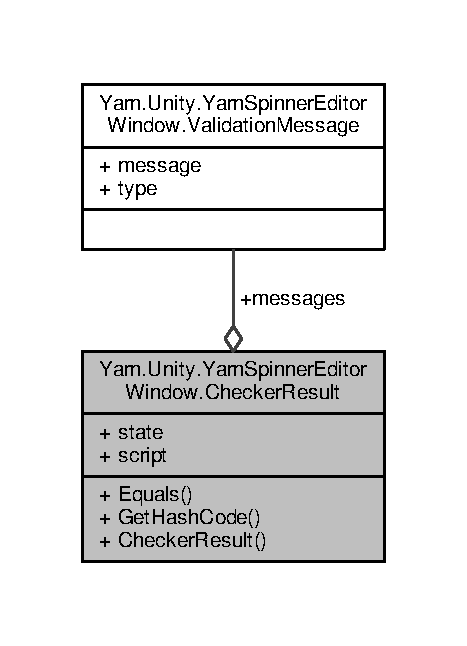
\includegraphics[width=224pt]{d7/d7e/a00709}
\end{center}
\end{figure}
\subsection*{Public Types}
\begin{DoxyCompactItemize}
\item 
enum \hyperlink{a00029_ab24848d7951ce44eb3c7768c6ee10385}{State} \{ \hyperlink{a00029_ab24848d7951ce44eb3c7768c6ee10385a0197c47523ba5a2bdfef705786687de5}{State.\-Not\-Tested}, 
\hyperlink{a00029_ab24848d7951ce44eb3c7768c6ee10385aa0d0628f6b4e4d78d2ffef4d4d1c4b15}{State.\-Passed}, 
\hyperlink{a00029_ab24848d7951ce44eb3c7768c6ee10385ad7c8c85bf79bbe1b7188497c32c3b0ca}{State.\-Failed}
 \}
\end{DoxyCompactItemize}
\subsection*{Public Member Functions}
\begin{DoxyCompactItemize}
\item 
override bool \hyperlink{a00029_a1e653caad5ab99847c26ff8f67da8f45}{Equals} (object obj)
\item 
override int \hyperlink{a00029_a85d50993390cdd8ba30ac44043b18de7}{Get\-Hash\-Code} ()
\item 
\hyperlink{a00029_af1c9b3d1757d33ad2141c639c3827c97}{Checker\-Result} (Text\-Asset \hyperlink{a00029_a6c852f7521c0a91b519aa3d391f63e6b}{script})
\end{DoxyCompactItemize}
\subsection*{Public Attributes}
\begin{DoxyCompactItemize}
\item 
\hyperlink{a00029_ab24848d7951ce44eb3c7768c6ee10385}{State} \hyperlink{a00029_a7202b24bd068da24d7e28bec5668b13a}{state}
\item 
Text\-Asset \hyperlink{a00029_a6c852f7521c0a91b519aa3d391f63e6b}{script}
\item 
\hyperlink{a00162_d4/d8f/a00324}{Validation\-Message}\mbox{[}$\,$\mbox{]} \hyperlink{a00029_a808a039e280cf875cb3c9e9385148498}{messages} = new \hyperlink{a00162_d4/d8f/a00324}{Validation\-Message}\mbox{[}0\mbox{]}
\end{DoxyCompactItemize}


\subsection{Detailed Description}


\subsection{Member Enumeration Documentation}
\hypertarget{a00029_ab24848d7951ce44eb3c7768c6ee10385}{\index{Yarn\-::\-Unity\-::\-Yarn\-Spinner\-Editor\-Window\-::\-Checker\-Result@{Yarn\-::\-Unity\-::\-Yarn\-Spinner\-Editor\-Window\-::\-Checker\-Result}!State@{State}}
\index{State@{State}!Yarn::Unity::YarnSpinnerEditorWindow::CheckerResult@{Yarn\-::\-Unity\-::\-Yarn\-Spinner\-Editor\-Window\-::\-Checker\-Result}}
\subsubsection[{State}]{\setlength{\rightskip}{0pt plus 5cm}enum {\bf Yarn.\-Unity.\-Yarn\-Spinner\-Editor\-Window.\-Checker\-Result.\-State}}}\label{a00029_ab24848d7951ce44eb3c7768c6ee10385}
\begin{Desc}
\item[Enumerator]\par
\begin{description}
\index{Not\-Tested@{Not\-Tested}!Yarn\-::\-Unity\-::\-Yarn\-Spinner\-Editor\-Window\-::\-Checker\-Result@{Yarn\-::\-Unity\-::\-Yarn\-Spinner\-Editor\-Window\-::\-Checker\-Result}}\index{Yarn\-::\-Unity\-::\-Yarn\-Spinner\-Editor\-Window\-::\-Checker\-Result@{Yarn\-::\-Unity\-::\-Yarn\-Spinner\-Editor\-Window\-::\-Checker\-Result}!Not\-Tested@{Not\-Tested}}\item[{\em 
\hypertarget{a00029_ab24848d7951ce44eb3c7768c6ee10385a0197c47523ba5a2bdfef705786687de5}{Not\-Tested}\label{a00029_ab24848d7951ce44eb3c7768c6ee10385a0197c47523ba5a2bdfef705786687de5}
}]\index{Passed@{Passed}!Yarn\-::\-Unity\-::\-Yarn\-Spinner\-Editor\-Window\-::\-Checker\-Result@{Yarn\-::\-Unity\-::\-Yarn\-Spinner\-Editor\-Window\-::\-Checker\-Result}}\index{Yarn\-::\-Unity\-::\-Yarn\-Spinner\-Editor\-Window\-::\-Checker\-Result@{Yarn\-::\-Unity\-::\-Yarn\-Spinner\-Editor\-Window\-::\-Checker\-Result}!Passed@{Passed}}\item[{\em 
\hypertarget{a00029_ab24848d7951ce44eb3c7768c6ee10385aa0d0628f6b4e4d78d2ffef4d4d1c4b15}{Passed}\label{a00029_ab24848d7951ce44eb3c7768c6ee10385aa0d0628f6b4e4d78d2ffef4d4d1c4b15}
}]\index{Failed@{Failed}!Yarn\-::\-Unity\-::\-Yarn\-Spinner\-Editor\-Window\-::\-Checker\-Result@{Yarn\-::\-Unity\-::\-Yarn\-Spinner\-Editor\-Window\-::\-Checker\-Result}}\index{Yarn\-::\-Unity\-::\-Yarn\-Spinner\-Editor\-Window\-::\-Checker\-Result@{Yarn\-::\-Unity\-::\-Yarn\-Spinner\-Editor\-Window\-::\-Checker\-Result}!Failed@{Failed}}\item[{\em 
\hypertarget{a00029_ab24848d7951ce44eb3c7768c6ee10385ad7c8c85bf79bbe1b7188497c32c3b0ca}{Failed}\label{a00029_ab24848d7951ce44eb3c7768c6ee10385ad7c8c85bf79bbe1b7188497c32c3b0ca}
}]\end{description}
\end{Desc}

\begin{DoxyCode}
36                               \{
37                 \hyperlink{a00029_ab24848d7951ce44eb3c7768c6ee10385a0197c47523ba5a2bdfef705786687de5}{NotTested},
38                 \hyperlink{a00029_ab24848d7951ce44eb3c7768c6ee10385aa0d0628f6b4e4d78d2ffef4d4d1c4b15}{Passed},
39                 \hyperlink{a00029_ab24848d7951ce44eb3c7768c6ee10385ad7c8c85bf79bbe1b7188497c32c3b0ca}{Failed}
40             \}
\end{DoxyCode}


\subsection{Constructor \& Destructor Documentation}
\hypertarget{a00029_af1c9b3d1757d33ad2141c639c3827c97}{\index{Yarn\-::\-Unity\-::\-Yarn\-Spinner\-Editor\-Window\-::\-Checker\-Result@{Yarn\-::\-Unity\-::\-Yarn\-Spinner\-Editor\-Window\-::\-Checker\-Result}!Checker\-Result@{Checker\-Result}}
\index{Checker\-Result@{Checker\-Result}!Yarn::Unity::YarnSpinnerEditorWindow::CheckerResult@{Yarn\-::\-Unity\-::\-Yarn\-Spinner\-Editor\-Window\-::\-Checker\-Result}}
\subsubsection[{Checker\-Result}]{\setlength{\rightskip}{0pt plus 5cm}Yarn.\-Unity.\-Yarn\-Spinner\-Editor\-Window.\-Checker\-Result.\-Checker\-Result (
\begin{DoxyParamCaption}
\item[{Text\-Asset}]{script}
\end{DoxyParamCaption}
)}}\label{a00029_af1c9b3d1757d33ad2141c639c3827c97}

\begin{DoxyCode}
60                                                    \{
61                 this.script = \hyperlink{a00029_a6c852f7521c0a91b519aa3d391f63e6b}{script};
62                 this.state = State.NotTested;
63             \}
\end{DoxyCode}


\subsection{Member Function Documentation}
\hypertarget{a00029_a1e653caad5ab99847c26ff8f67da8f45}{\index{Yarn\-::\-Unity\-::\-Yarn\-Spinner\-Editor\-Window\-::\-Checker\-Result@{Yarn\-::\-Unity\-::\-Yarn\-Spinner\-Editor\-Window\-::\-Checker\-Result}!Equals@{Equals}}
\index{Equals@{Equals}!Yarn::Unity::YarnSpinnerEditorWindow::CheckerResult@{Yarn\-::\-Unity\-::\-Yarn\-Spinner\-Editor\-Window\-::\-Checker\-Result}}
\subsubsection[{Equals}]{\setlength{\rightskip}{0pt plus 5cm}override bool Yarn.\-Unity.\-Yarn\-Spinner\-Editor\-Window.\-Checker\-Result.\-Equals (
\begin{DoxyParamCaption}
\item[{object}]{obj}
\end{DoxyParamCaption}
)}}\label{a00029_a1e653caad5ab99847c26ff8f67da8f45}

\begin{DoxyCode}
48             \{
49                 \textcolor{keywordflow}{if} (obj is \hyperlink{a00029_af1c9b3d1757d33ad2141c639c3827c97}{CheckerResult} && ((\hyperlink{a00029_af1c9b3d1757d33ad2141c639c3827c97}{CheckerResult})obj).
      \hyperlink{a00029_a6c852f7521c0a91b519aa3d391f63e6b}{script} == this.\hyperlink{a00029_a6c852f7521c0a91b519aa3d391f63e6b}{script})
50                     \textcolor{keywordflow}{return} \textcolor{keyword}{true};
51                 \textcolor{keywordflow}{else}
52                     \textcolor{keywordflow}{return} \textcolor{keyword}{false};
53             \}
\end{DoxyCode}
\hypertarget{a00029_a85d50993390cdd8ba30ac44043b18de7}{\index{Yarn\-::\-Unity\-::\-Yarn\-Spinner\-Editor\-Window\-::\-Checker\-Result@{Yarn\-::\-Unity\-::\-Yarn\-Spinner\-Editor\-Window\-::\-Checker\-Result}!Get\-Hash\-Code@{Get\-Hash\-Code}}
\index{Get\-Hash\-Code@{Get\-Hash\-Code}!Yarn::Unity::YarnSpinnerEditorWindow::CheckerResult@{Yarn\-::\-Unity\-::\-Yarn\-Spinner\-Editor\-Window\-::\-Checker\-Result}}
\subsubsection[{Get\-Hash\-Code}]{\setlength{\rightskip}{0pt plus 5cm}override int Yarn.\-Unity.\-Yarn\-Spinner\-Editor\-Window.\-Checker\-Result.\-Get\-Hash\-Code (
\begin{DoxyParamCaption}
{}
\end{DoxyParamCaption}
)}}\label{a00029_a85d50993390cdd8ba30ac44043b18de7}

\begin{DoxyCode}
56             \{
57                 \textcolor{keywordflow}{return} this.script.GetHashCode();
58             \}
\end{DoxyCode}


\subsection{Member Data Documentation}
\hypertarget{a00029_a808a039e280cf875cb3c9e9385148498}{\index{Yarn\-::\-Unity\-::\-Yarn\-Spinner\-Editor\-Window\-::\-Checker\-Result@{Yarn\-::\-Unity\-::\-Yarn\-Spinner\-Editor\-Window\-::\-Checker\-Result}!messages@{messages}}
\index{messages@{messages}!Yarn::Unity::YarnSpinnerEditorWindow::CheckerResult@{Yarn\-::\-Unity\-::\-Yarn\-Spinner\-Editor\-Window\-::\-Checker\-Result}}
\subsubsection[{messages}]{\setlength{\rightskip}{0pt plus 5cm}{\bf Validation\-Message} \mbox{[}$\,$\mbox{]} Yarn.\-Unity.\-Yarn\-Spinner\-Editor\-Window.\-Checker\-Result.\-messages = new {\bf Validation\-Message}\mbox{[}0\mbox{]}}}\label{a00029_a808a039e280cf875cb3c9e9385148498}
\hypertarget{a00029_a6c852f7521c0a91b519aa3d391f63e6b}{\index{Yarn\-::\-Unity\-::\-Yarn\-Spinner\-Editor\-Window\-::\-Checker\-Result@{Yarn\-::\-Unity\-::\-Yarn\-Spinner\-Editor\-Window\-::\-Checker\-Result}!script@{script}}
\index{script@{script}!Yarn::Unity::YarnSpinnerEditorWindow::CheckerResult@{Yarn\-::\-Unity\-::\-Yarn\-Spinner\-Editor\-Window\-::\-Checker\-Result}}
\subsubsection[{script}]{\setlength{\rightskip}{0pt plus 5cm}Text\-Asset Yarn.\-Unity.\-Yarn\-Spinner\-Editor\-Window.\-Checker\-Result.\-script}}\label{a00029_a6c852f7521c0a91b519aa3d391f63e6b}
\hypertarget{a00029_a7202b24bd068da24d7e28bec5668b13a}{\index{Yarn\-::\-Unity\-::\-Yarn\-Spinner\-Editor\-Window\-::\-Checker\-Result@{Yarn\-::\-Unity\-::\-Yarn\-Spinner\-Editor\-Window\-::\-Checker\-Result}!state@{state}}
\index{state@{state}!Yarn::Unity::YarnSpinnerEditorWindow::CheckerResult@{Yarn\-::\-Unity\-::\-Yarn\-Spinner\-Editor\-Window\-::\-Checker\-Result}}
\subsubsection[{state}]{\setlength{\rightskip}{0pt plus 5cm}{\bf State} Yarn.\-Unity.\-Yarn\-Spinner\-Editor\-Window.\-Checker\-Result.\-state}}\label{a00029_a7202b24bd068da24d7e28bec5668b13a}


The documentation for this class was generated from the following file\-:\begin{DoxyCompactItemize}
\item 
Unity/\-Assets/\-Yarn Spinner/\-Code/\-Editor/\hyperlink{a00254}{Yarn\-Spinner\-Editor\-Window.\-cs}\end{DoxyCompactItemize}

The M\-I\-T License (M\-I\-T)

Copyright (c) 2015-\/2017 Secret Lab Pty. Ltd. and \hyperlink{a00040}{Yarn} Spinner contributors.

Permission is hereby granted, free of charge, to any person obtaining a copy of this software and associated documentation files (the \char`\"{}\-Software\char`\"{}), to deal in the Software without restriction, including without limitation the rights to use, copy, modify, merge, publish, distribute, sublicense, and/or sell copies of the Software, and to permit persons to whom the Software is furnished to do so, subject to the following conditions\-:

The above copyright notice and this permission notice shall be included in all copies or substantial portions of the Software.

T\-H\-E S\-O\-F\-T\-W\-A\-R\-E I\-S P\-R\-O\-V\-I\-D\-E\-D \char`\"{}\-A\-S I\-S\char`\"{}, W\-I\-T\-H\-O\-U\-T W\-A\-R\-R\-A\-N\-T\-Y O\-F A\-N\-Y K\-I\-N\-D, E\-X\-P\-R\-E\-S\-S O\-R I\-M\-P\-L\-I\-E\-D, I\-N\-C\-L\-U\-D\-I\-N\-G B\-U\-T N\-O\-T L\-I\-M\-I\-T\-E\-D T\-O T\-H\-E W\-A\-R\-R\-A\-N\-T\-I\-E\-S O\-F M\-E\-R\-C\-H\-A\-N\-T\-A\-B\-I\-L\-I\-T\-Y, F\-I\-T\-N\-E\-S\-S F\-O\-R A P\-A\-R\-T\-I\-C\-U\-L\-A\-R P\-U\-R\-P\-O\-S\-E A\-N\-D N\-O\-N\-I\-N\-F\-R\-I\-N\-G\-E\-M\-E\-N\-T. I\-N N\-O E\-V\-E\-N\-T S\-H\-A\-L\-L T\-H\-E A\-U\-T\-H\-O\-R\-S O\-R C\-O\-P\-Y\-R\-I\-G\-H\-T H\-O\-L\-D\-E\-R\-S B\-E L\-I\-A\-B\-L\-E F\-O\-R A\-N\-Y C\-L\-A\-I\-M, D\-A\-M\-A\-G\-E\-S O\-R O\-T\-H\-E\-R L\-I\-A\-B\-I\-L\-I\-T\-Y, W\-H\-E\-T\-H\-E\-R I\-N A\-N A\-C\-T\-I\-O\-N O\-F C\-O\-N\-T\-R\-A\-C\-T, T\-O\-R\-T O\-R O\-T\-H\-E\-R\-W\-I\-S\-E, A\-R\-I\-S\-I\-N\-G F\-R\-O\-M, O\-U\-T O\-F O\-R I\-N C\-O\-N\-N\-E\-C\-T\-I\-O\-N W\-I\-T\-H T\-H\-E S\-O\-F\-T\-W\-A\-R\-E O\-R T\-H\-E U\-S\-E O\-R O\-T\-H\-E\-R D\-E\-A\-L\-I\-N\-G\-S I\-N T\-H\-E S\-O\-F\-T\-W\-A\-R\-E.

This software contains third-\/party code\-: Unity Test Tools (M\-I\-T license), N\-Unit (B\-S\-D license), N\-Substitute (B\-S\-D license) and Cecil (M\-I\-T/\-X11 license). For more information, see the \href{Unity/Assets/UnityTestTools/LICENSE.txt}{\tt Unity Test Tools license file}. 
\hypertarget{a00031}{\section{Yarn.\-Analysis.\-Compiled\-Program\-Analyser Class Reference}
\label{a00031}\index{Yarn.\-Analysis.\-Compiled\-Program\-Analyser@{Yarn.\-Analysis.\-Compiled\-Program\-Analyser}}
}


Inheritance diagram for Yarn.\-Analysis.\-Compiled\-Program\-Analyser\-:
\nopagebreak
\begin{figure}[H]
\begin{center}
\leavevmode
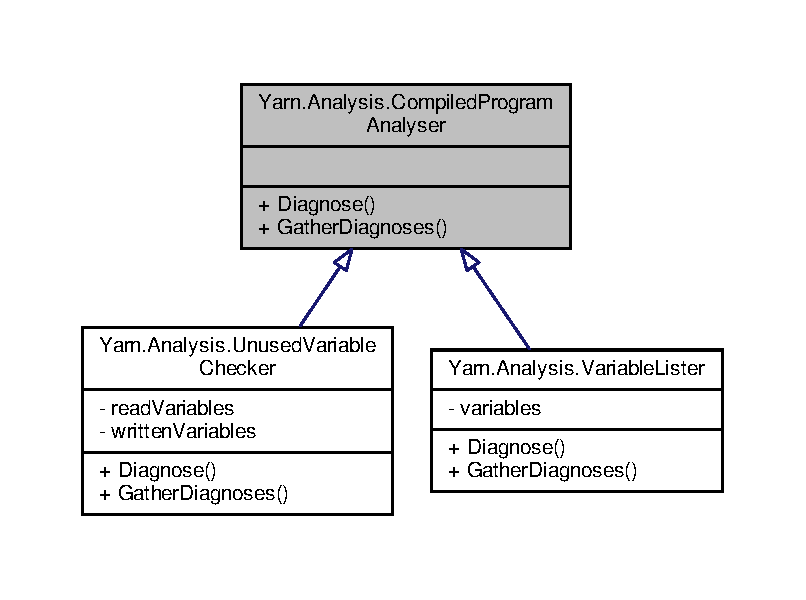
\includegraphics[width=350pt]{d7/dc3/a00682}
\end{center}
\end{figure}


Collaboration diagram for Yarn.\-Analysis.\-Compiled\-Program\-Analyser\-:
\nopagebreak
\begin{figure}[H]
\begin{center}
\leavevmode
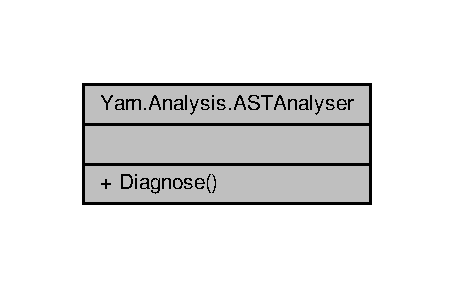
\includegraphics[width=236pt]{db/d77/a00683}
\end{center}
\end{figure}
\subsection*{Public Member Functions}
\begin{DoxyCompactItemize}
\item 
abstract void \hyperlink{a00031_aba4a36cb823b11ee491074e26477d084}{Diagnose} (\hyperlink{a00124}{Yarn.\-Program} program)
\item 
abstract I\-Enumerable$<$ \hyperlink{a00069}{Diagnosis} $>$ \hyperlink{a00031_afe059a2ceeabe50380b000420e512bd6}{Gather\-Diagnoses} ()
\end{DoxyCompactItemize}


\subsection{Detailed Description}


\subsection{Member Function Documentation}
\hypertarget{a00031_aba4a36cb823b11ee491074e26477d084}{\index{Yarn\-::\-Analysis\-::\-Compiled\-Program\-Analyser@{Yarn\-::\-Analysis\-::\-Compiled\-Program\-Analyser}!Diagnose@{Diagnose}}
\index{Diagnose@{Diagnose}!Yarn::Analysis::CompiledProgramAnalyser@{Yarn\-::\-Analysis\-::\-Compiled\-Program\-Analyser}}
\subsubsection[{Diagnose}]{\setlength{\rightskip}{0pt plus 5cm}abstract void Yarn.\-Analysis.\-Compiled\-Program\-Analyser.\-Diagnose (
\begin{DoxyParamCaption}
\item[{{\bf Yarn.\-Program}}]{program}
\end{DoxyParamCaption}
)\hspace{0.3cm}{\ttfamily [pure virtual]}}}\label{a00031_aba4a36cb823b11ee491074e26477d084}
\hypertarget{a00031_afe059a2ceeabe50380b000420e512bd6}{\index{Yarn\-::\-Analysis\-::\-Compiled\-Program\-Analyser@{Yarn\-::\-Analysis\-::\-Compiled\-Program\-Analyser}!Gather\-Diagnoses@{Gather\-Diagnoses}}
\index{Gather\-Diagnoses@{Gather\-Diagnoses}!Yarn::Analysis::CompiledProgramAnalyser@{Yarn\-::\-Analysis\-::\-Compiled\-Program\-Analyser}}
\subsubsection[{Gather\-Diagnoses}]{\setlength{\rightskip}{0pt plus 5cm}abstract I\-Enumerable$<${\bf Diagnosis}$>$ Yarn.\-Analysis.\-Compiled\-Program\-Analyser.\-Gather\-Diagnoses (
\begin{DoxyParamCaption}
{}
\end{DoxyParamCaption}
)\hspace{0.3cm}{\ttfamily [pure virtual]}}}\label{a00031_afe059a2ceeabe50380b000420e512bd6}


Implemented in \hyperlink{a00159_a107aecf707b130c4b733930a95f9154e}{Yarn.\-Analysis.\-Unused\-Variable\-Checker}, and \hyperlink{a00163_ab84e7a8e68740379dee12a51dca69b07}{Yarn.\-Analysis.\-Variable\-Lister}.



The documentation for this class was generated from the following file\-:\begin{DoxyCompactItemize}
\item 
Yarn\-Spinner/\hyperlink{a00260}{Analyser.\-cs}\end{DoxyCompactItemize}

\hypertarget{a00032}{\section{Yarn.\-Dialogue.\-Command\-Result Class Reference}
\label{a00032}\index{Yarn.\-Dialogue.\-Command\-Result@{Yarn.\-Dialogue.\-Command\-Result}}
}


Inheritance diagram for Yarn.\-Dialogue.\-Command\-Result\-:
\nopagebreak
\begin{figure}[H]
\begin{center}
\leavevmode
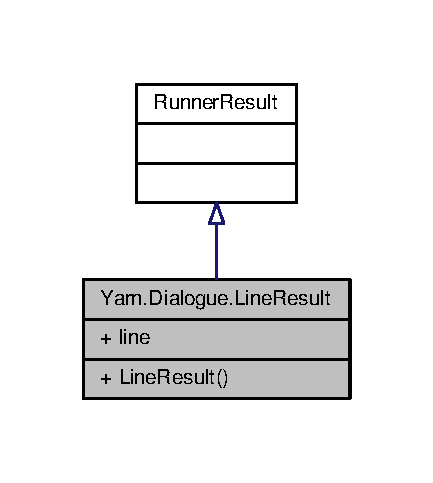
\includegraphics[width=234pt]{d8/deb/a00545}
\end{center}
\end{figure}


Collaboration diagram for Yarn.\-Dialogue.\-Command\-Result\-:
\nopagebreak
\begin{figure}[H]
\begin{center}
\leavevmode
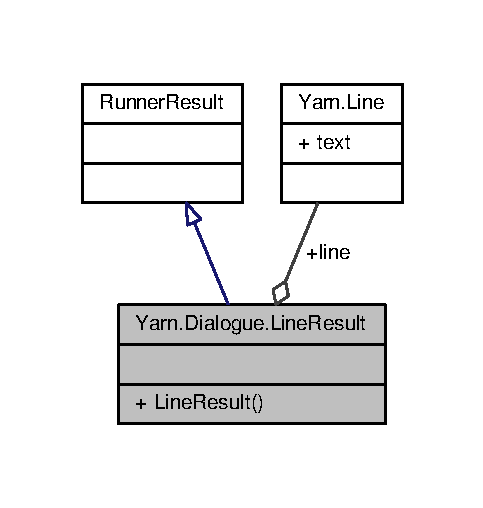
\includegraphics[width=259pt]{dc/d2b/a00546}
\end{center}
\end{figure}
\subsection*{Public Member Functions}
\begin{DoxyCompactItemize}
\item 
\hyperlink{a00032_a1a553422394fb0c854d1184985f993bb}{Command\-Result} (string text)
\end{DoxyCompactItemize}
\subsection*{Public Attributes}
\begin{DoxyCompactItemize}
\item 
\hyperlink{a00031_d4/d6f/a00315}{Command} \hyperlink{a00032_a420ca0984d6e5c33bb761654305c592e}{command}
\end{DoxyCompactItemize}


\subsection{Detailed Description}


\subsection{Constructor \& Destructor Documentation}
\hypertarget{a00032_a1a553422394fb0c854d1184985f993bb}{\index{Yarn\-::\-Dialogue\-::\-Command\-Result@{Yarn\-::\-Dialogue\-::\-Command\-Result}!Command\-Result@{Command\-Result}}
\index{Command\-Result@{Command\-Result}!Yarn::Dialogue::CommandResult@{Yarn\-::\-Dialogue\-::\-Command\-Result}}
\subsubsection[{Command\-Result}]{\setlength{\rightskip}{0pt plus 5cm}Yarn.\-Dialogue.\-Command\-Result.\-Command\-Result (
\begin{DoxyParamCaption}
\item[{string}]{text}
\end{DoxyParamCaption}
)}}\label{a00032_a1a553422394fb0c854d1184985f993bb}

\begin{DoxyCode}
146                                                \{
147                 var \hyperlink{a00032_a420ca0984d6e5c33bb761654305c592e}{command} = \textcolor{keyword}{new} Command();
148                 command.text = text;
149                 this.command = \hyperlink{a00032_a420ca0984d6e5c33bb761654305c592e}{command};
150             \}
\end{DoxyCode}


\subsection{Member Data Documentation}
\hypertarget{a00032_a420ca0984d6e5c33bb761654305c592e}{\index{Yarn\-::\-Dialogue\-::\-Command\-Result@{Yarn\-::\-Dialogue\-::\-Command\-Result}!command@{command}}
\index{command@{command}!Yarn::Dialogue::CommandResult@{Yarn\-::\-Dialogue\-::\-Command\-Result}}
\subsubsection[{command}]{\setlength{\rightskip}{0pt plus 5cm}{\bf Command} Yarn.\-Dialogue.\-Command\-Result.\-command}}\label{a00032_a420ca0984d6e5c33bb761654305c592e}


The documentation for this class was generated from the following file\-:\begin{DoxyCompactItemize}
\item 
Yarn\-Spinner/\hyperlink{a00265}{Dialogue.\-cs}\end{DoxyCompactItemize}

\hypertarget{a00034}{\section{Yarn.\-Compiler Class Reference}
\label{a00034}\index{Yarn.\-Compiler@{Yarn.\-Compiler}}
}


Collaboration diagram for Yarn.\-Compiler\-:
\nopagebreak
\begin{figure}[H]
\begin{center}
\leavevmode
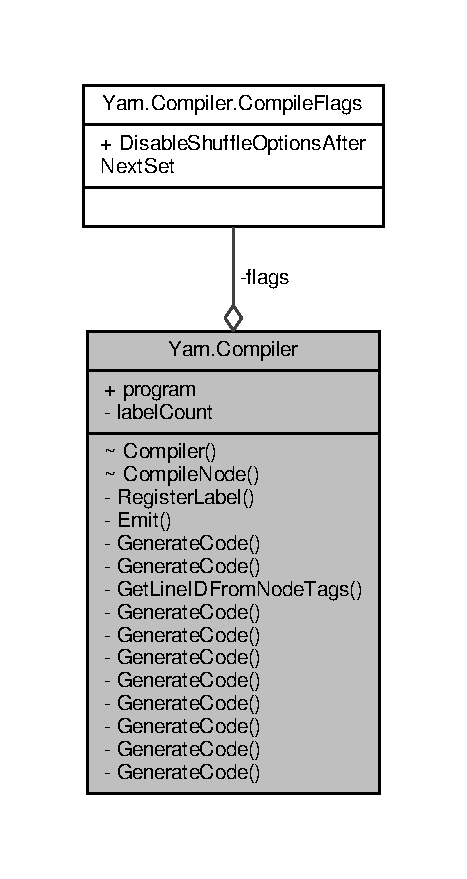
\includegraphics[width=224pt]{d9/d44/a00527}
\end{center}
\end{figure}
\subsection*{Classes}
\begin{DoxyCompactItemize}
\item 
struct \hyperlink{a00034_d3/db8/a00316}{Compile\-Flags}
\end{DoxyCompactItemize}
\subsection*{Package Functions}
\begin{DoxyCompactItemize}
\item 
\hyperlink{a00034_a47bfde319a618a1e11d00cb282a84364}{Compiler} (string program\-Name)
\item 
void \hyperlink{a00034_a10b52c5694f78285d087a455e3654eaa}{Compile\-Node} (\hyperlink{a00112}{Parser.\-Node} node)
\end{DoxyCompactItemize}
\subsection*{Properties}
\begin{DoxyCompactItemize}
\item 
\hyperlink{a00126}{Program} \hyperlink{a00034_aa1737da428ec7d597009661dd8a47829}{program}\hspace{0.3cm}{\ttfamily  \mbox{[}get, set\mbox{]}}
\end{DoxyCompactItemize}
\subsection*{Private Member Functions}
\begin{DoxyCompactItemize}
\item 
string \hyperlink{a00034_a1bae0d8b701a59708641aa36ea971fa5}{Register\-Label} (string commentary=null)
\item 
void \hyperlink{a00034_a774e8c143cdda0584fcfdda98626a83c}{Emit} (\hyperlink{a00031_dd/de2/a00320}{Node} node, \hyperlink{a00031_ad5dfb6ee68ca7469623ad3e459f98894}{Byte\-Code} code, object operand\-A=null, object operand\-B=null)
\item 
void \hyperlink{a00034_a006f3becd521cc179ba3d3352f6f930b}{Generate\-Code} (\hyperlink{a00031_dd/de2/a00320}{Node} node, \hyperlink{a00142}{Parser.\-Statement} statement)
\item 
void \hyperlink{a00034_a656b6c7fcd08d24300ec592465274f66}{Generate\-Code} (\hyperlink{a00031_dd/de2/a00320}{Node} node, \hyperlink{a00063}{Parser.\-Custom\-Command} statement)
\item 
string \hyperlink{a00034_a5117b9c2253de15d3fd3557c8b037235}{Get\-Line\-I\-D\-From\-Node\-Tags} (\hyperlink{a00122}{Parser.\-Parse\-Node} node)
\item 
void \hyperlink{a00034_af1ee28d67902b27ee0816e2a47343652}{Generate\-Code} (\hyperlink{a00031_dd/de2/a00320}{Node} node, \hyperlink{a00142}{Parser.\-Statement} parse\-Node, string line)
\item 
void \hyperlink{a00034_a3e492edcefdfeacec80e528f8c4fa6cc}{Generate\-Code} (\hyperlink{a00031_dd/de2/a00320}{Node} node, \hyperlink{a00136}{Parser.\-Shortcut\-Option\-Group} statement)
\item 
void \hyperlink{a00034_ab4f6dd2ddf38b0c5bfb2b8a40869a09a}{Generate\-Code} (\hyperlink{a00031_dd/de2/a00320}{Node} node, I\-Enumerable$<$ \hyperlink{a00142}{Yarn.\-Parser.\-Statement} $>$ statement\-List)
\item 
void \hyperlink{a00034_a6ab14514a3b0644ae39c626e5e5e180d}{Generate\-Code} (\hyperlink{a00031_dd/de2/a00320}{Node} node, \hyperlink{a00094}{Parser.\-If\-Statement} statement)
\item 
void \hyperlink{a00034_a5cb3cbcd9727bdef018ec5299bd13142}{Generate\-Code} (\hyperlink{a00031_dd/de2/a00320}{Node} node, \hyperlink{a00120}{Parser.\-Option\-Statement} statement)
\item 
void \hyperlink{a00034_afb86d9228f66896abe31d47d72a267ce}{Generate\-Code} (\hyperlink{a00031_dd/de2/a00320}{Node} node, \hyperlink{a00020}{Parser.\-Assignment\-Statement} statement)
\item 
void \hyperlink{a00034_a5c762915320958c3a03b193b06a7e279}{Generate\-Code} (\hyperlink{a00031_dd/de2/a00320}{Node} node, \hyperlink{a00082}{Parser.\-Expression} expression)
\item 
void \hyperlink{a00034_a41438a0b25f2668a180372d05127d891}{Generate\-Code} (\hyperlink{a00031_dd/de2/a00320}{Node} node, \hyperlink{a00164}{Parser.\-Value\-Node} value)
\end{DoxyCompactItemize}
\subsection*{Private Attributes}
\begin{DoxyCompactItemize}
\item 
\hyperlink{a00034_d3/db8/a00316}{Compile\-Flags} \hyperlink{a00034_a541022d89bcf9bc8f794eb6d6b438d08}{flags}
\item 
int \hyperlink{a00034_a87758397eba2e84cda8e0d6c40656f3f}{label\-Count} = 0
\end{DoxyCompactItemize}


\subsection{Detailed Description}


\subsection{Class Documentation}
\index{Yarn\-::\-Compiler\-::\-Compile\-Flags@{Yarn\-::\-Compiler\-::\-Compile\-Flags}}\label{d3/db8/a00316}
\hypertarget{a00034_d3/db8/a00316}{}
\subsubsection{struct Yarn\-:\-:Compiler\-:\-:Compile\-Flags}


Collaboration diagram for Yarn.\-Compiler.\-Compile\-Flags\-:
\nopagebreak
\begin{figure}[H]
\begin{center}
\leavevmode
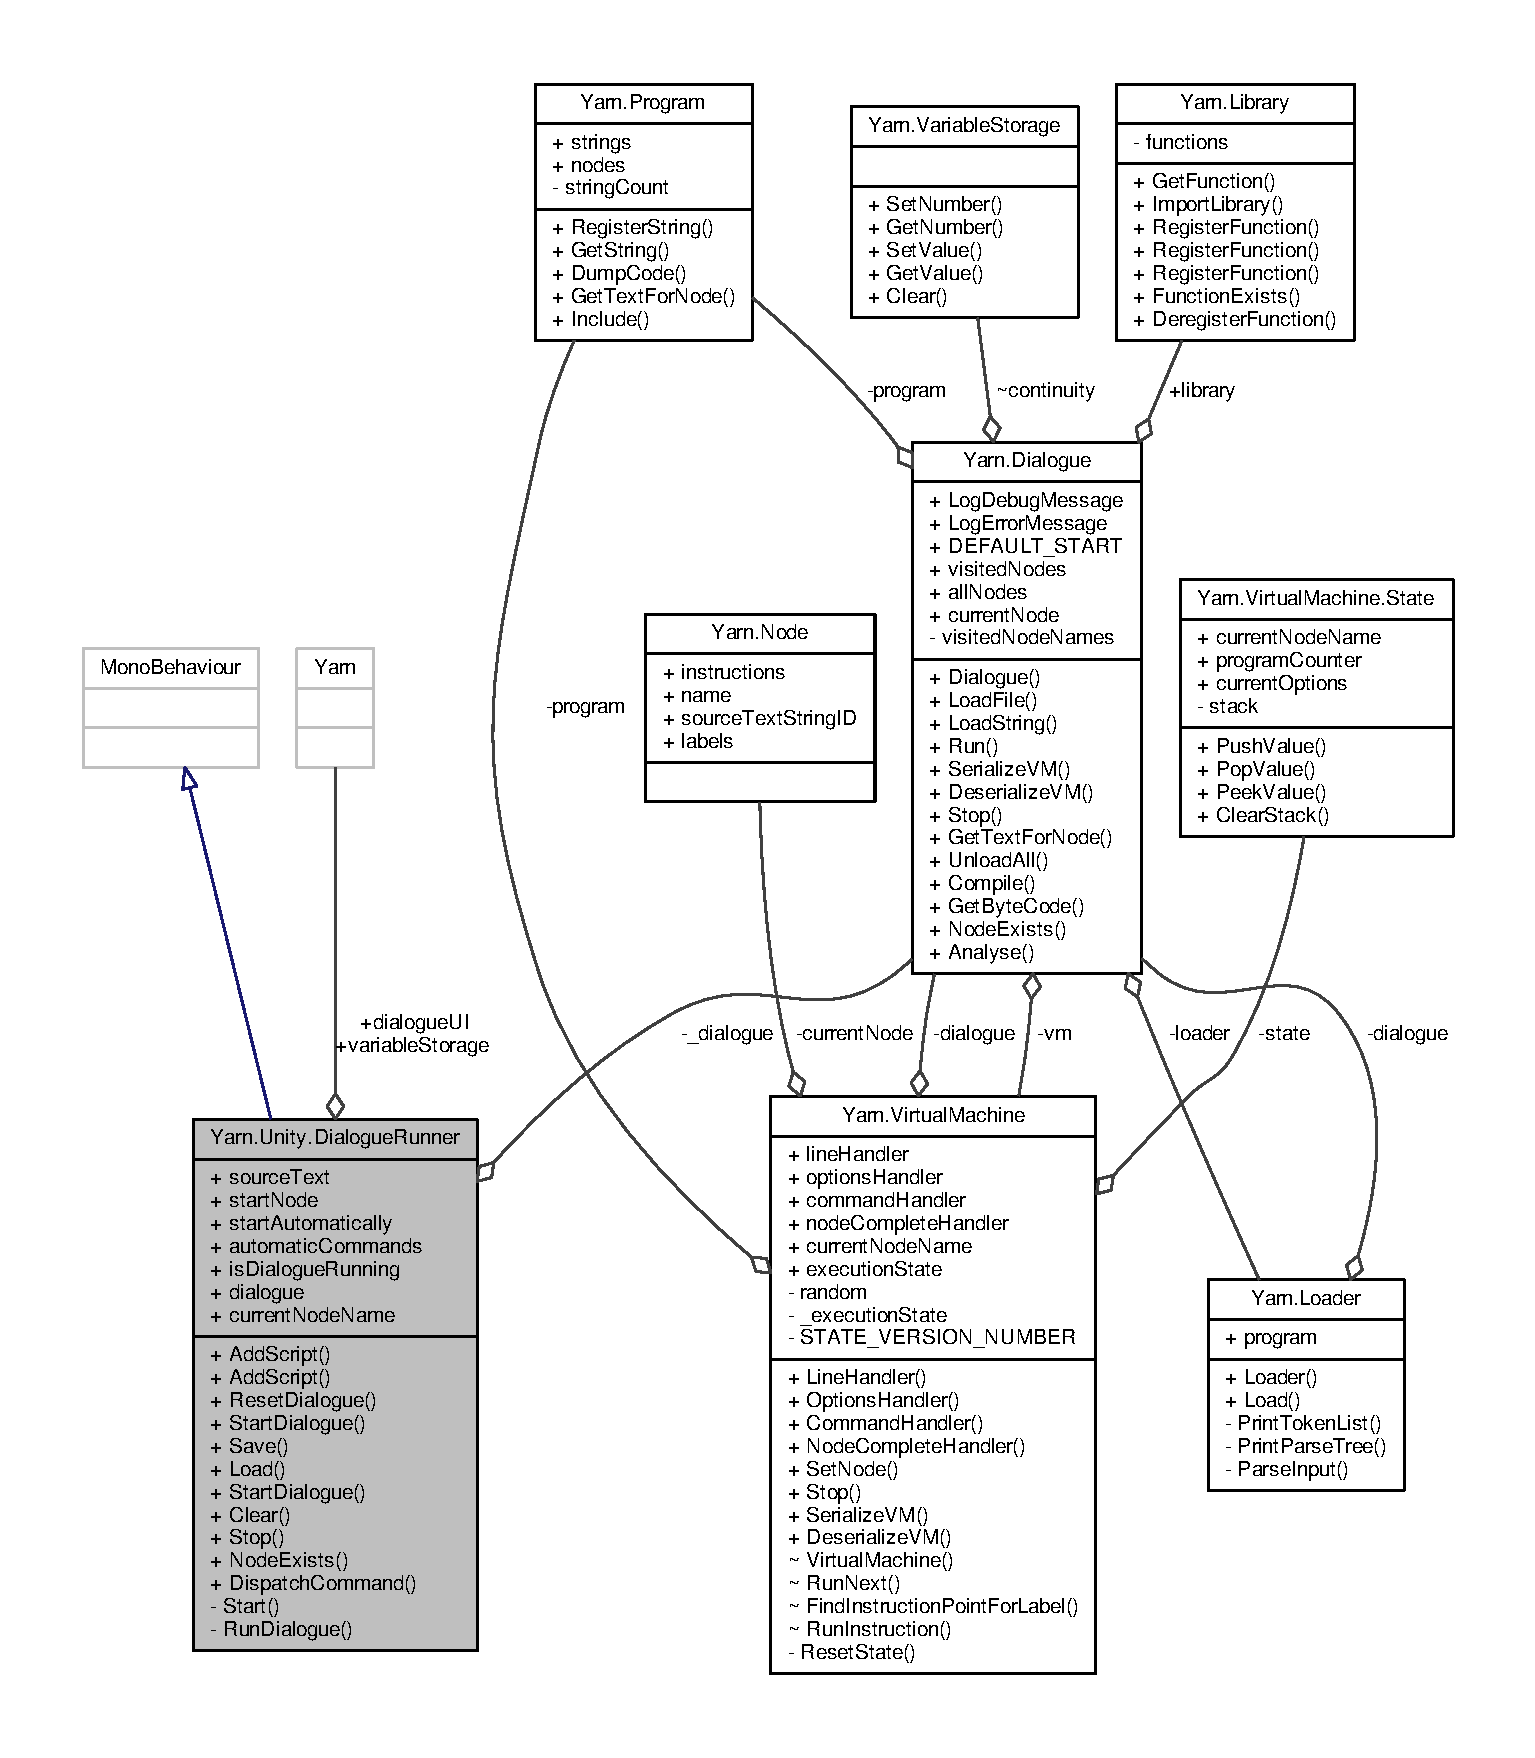
\includegraphics[width=224pt]{dd/dbb/a00330}
\end{center}
\end{figure}
\begin{DoxyFields}{Class Members}
\hypertarget{a00034_a8b49bb7763ff477cba21d7c771ef3ed0}{bool}\label{a00034_a8b49bb7763ff477cba21d7c771ef3ed0}
&
Disable\-Shuffle\-Options\-After\-Next\-Set&
\\
\hline

\end{DoxyFields}


\subsection{Constructor \& Destructor Documentation}
\hypertarget{a00034_a47bfde319a618a1e11d00cb282a84364}{\index{Yarn\-::\-Compiler@{Yarn\-::\-Compiler}!Compiler@{Compiler}}
\index{Compiler@{Compiler}!Yarn::Compiler@{Yarn\-::\-Compiler}}
\subsubsection[{Compiler}]{\setlength{\rightskip}{0pt plus 5cm}Yarn.\-Compiler.\-Compiler (
\begin{DoxyParamCaption}
\item[{string}]{program\-Name}
\end{DoxyParamCaption}
)\hspace{0.3cm}{\ttfamily [package]}}}\label{a00034_a47bfde319a618a1e11d00cb282a84364}

\begin{DoxyCode}
309         \{
310             \hyperlink{a00034_aa1737da428ec7d597009661dd8a47829}{program} = \textcolor{keyword}{new} Program ();
311         \}
\end{DoxyCode}


\subsection{Member Function Documentation}
\hypertarget{a00034_a10b52c5694f78285d087a455e3654eaa}{\index{Yarn\-::\-Compiler@{Yarn\-::\-Compiler}!Compile\-Node@{Compile\-Node}}
\index{Compile\-Node@{Compile\-Node}!Yarn::Compiler@{Yarn\-::\-Compiler}}
\subsubsection[{Compile\-Node}]{\setlength{\rightskip}{0pt plus 5cm}void Yarn.\-Compiler.\-Compile\-Node (
\begin{DoxyParamCaption}
\item[{{\bf Parser.\-Node}}]{node}
\end{DoxyParamCaption}
)\hspace{0.3cm}{\ttfamily [package]}}}\label{a00034_a10b52c5694f78285d087a455e3654eaa}

\begin{DoxyCode}
316                                                     \{
317 
318             \textcolor{keywordflow}{if} (\hyperlink{a00034_aa1737da428ec7d597009661dd8a47829}{program}.\hyperlink{a00126_a3f4928a577c88263ad016be259b175c4}{nodes}.ContainsKey(node.name)) \{
319                 \textcolor{keywordflow}{throw} \textcolor{keyword}{new} ArgumentException (\textcolor{stringliteral}{"Duplicate node name "} + node.name);
320             \}
321 
322             var compiledNode =  \textcolor{keyword}{new} Node();
323 
324             compiledNode.name = node.name;
325 
326             compiledNode.tags = node.nodeTags;
327 
328             \textcolor{comment}{// Register the entire text of this node if we have it}
329             \textcolor{keywordflow}{if} (node.source != null)
330             \{
331                 \textcolor{comment}{// Dump the entire contents of this node into the string table }
332                 \textcolor{comment}{// instead of compiling its contents.}
333 
334                 \textcolor{comment}{// the line number is 0 because the string starts at the start of the node}
335                 compiledNode.sourceTextStringID = program.RegisterString(node.source, node.name, \textcolor{stringliteral}{"line:"}+
      node.name, 0, \textcolor{keyword}{true});
336             \} \textcolor{keywordflow}{else} \{
337 
338                 \textcolor{comment}{// Compile the node.}
339 
340                 var startLabel = \hyperlink{a00034_a1bae0d8b701a59708641aa36ea971fa5}{RegisterLabel}();
341                 \hyperlink{a00034_a774e8c143cdda0584fcfdda98626a83c}{Emit}(compiledNode, \hyperlink{a00031_ad5dfb6ee68ca7469623ad3e459f98894}{ByteCode}.Label, startLabel);
342 
343                 \textcolor{keywordflow}{foreach} (var statement \textcolor{keywordflow}{in} node.statements)
344                 \{
345                     \hyperlink{a00034_a006f3becd521cc179ba3d3352f6f930b}{GenerateCode}(compiledNode, statement);
346                 \}
347 
348                 \textcolor{comment}{// Does this node end after emitting AddOptions codes}
349                 \textcolor{comment}{// without calling ShowOptions?}
350 
351                 \textcolor{comment}{// Note: this only works when we know that we don't have}
352                 \textcolor{comment}{// AddOptions and then Jump up back into the code to run them.}
353                 \textcolor{comment}{// TODO: A better solution would be for the parser to flag}
354                 \textcolor{comment}{// whether a node has Options at the end.}
355                 var hasRemainingOptions = \textcolor{keyword}{false};
356                 \textcolor{keywordflow}{foreach} (var instruction \textcolor{keywordflow}{in} compiledNode.instructions)
357                 \{
358                     \textcolor{keywordflow}{if} (instruction.operation == \hyperlink{a00031_ad5dfb6ee68ca7469623ad3e459f98894}{ByteCode}.AddOption)
359                     \{
360                         hasRemainingOptions = \textcolor{keyword}{true};
361                     \}
362                     \textcolor{keywordflow}{if} (instruction.operation == \hyperlink{a00031_ad5dfb6ee68ca7469623ad3e459f98894}{ByteCode}.ShowOptions)
363                     \{
364                         hasRemainingOptions = \textcolor{keyword}{false};
365                     \}
366                 \}
367 
368                 \textcolor{comment}{// If this compiled node has no lingering options to show at the end of the node, then stop
       at the end}
369                 \textcolor{keywordflow}{if} (hasRemainingOptions == \textcolor{keyword}{false})
370                 \{
371                     \hyperlink{a00034_a774e8c143cdda0584fcfdda98626a83c}{Emit}(compiledNode, \hyperlink{a00031_ad5dfb6ee68ca7469623ad3e459f98894}{ByteCode}.Stop);
372                 \}
373                 \textcolor{keywordflow}{else} \{
374                     \textcolor{comment}{// Otherwise, show the accumulated nodes and then jump to the selected node}
375 
376                     \hyperlink{a00034_a774e8c143cdda0584fcfdda98626a83c}{Emit}(compiledNode, \hyperlink{a00031_ad5dfb6ee68ca7469623ad3e459f98894}{ByteCode}.ShowOptions);
377 
378                     \textcolor{keywordflow}{if} (\hyperlink{a00034_a541022d89bcf9bc8f794eb6d6b438d08}{flags}.\hyperlink{a00034_a8b49bb7763ff477cba21d7c771ef3ed0}{DisableShuffleOptionsAfterNextSet} == \textcolor{keyword}{
      true})
379                     \{
380                         \hyperlink{a00034_a774e8c143cdda0584fcfdda98626a83c}{Emit}(compiledNode, \hyperlink{a00031_ad5dfb6ee68ca7469623ad3e459f98894}{ByteCode}.PushBool, \textcolor{keyword}{false});
381                         \hyperlink{a00034_a774e8c143cdda0584fcfdda98626a83c}{Emit}(compiledNode, \hyperlink{a00031_ad5dfb6ee68ca7469623ad3e459f98894}{ByteCode}.StoreVariable, VirtualMachine.
      SpecialVariables.ShuffleOptions);
382                         \hyperlink{a00034_a774e8c143cdda0584fcfdda98626a83c}{Emit}(compiledNode, \hyperlink{a00031_ad5dfb6ee68ca7469623ad3e459f98894}{ByteCode}.Pop);
383                         flags.DisableShuffleOptionsAfterNextSet = \textcolor{keyword}{false};
384                     \}
385 
386                     \hyperlink{a00034_a774e8c143cdda0584fcfdda98626a83c}{Emit}(compiledNode, \hyperlink{a00031_ad5dfb6ee68ca7469623ad3e459f98894}{ByteCode}.RunNode);
387                 \}
388 
389             \}
390 
391             program.nodes[compiledNode.name] = compiledNode;
392 
393         \}
\end{DoxyCode}
\hypertarget{a00034_a774e8c143cdda0584fcfdda98626a83c}{\index{Yarn\-::\-Compiler@{Yarn\-::\-Compiler}!Emit@{Emit}}
\index{Emit@{Emit}!Yarn::Compiler@{Yarn\-::\-Compiler}}
\subsubsection[{Emit}]{\setlength{\rightskip}{0pt plus 5cm}void Yarn.\-Compiler.\-Emit (
\begin{DoxyParamCaption}
\item[{{\bf Node}}]{node, }
\item[{{\bf Byte\-Code}}]{code, }
\item[{object}]{operand\-A = {\ttfamily null}, }
\item[{object}]{operand\-B = {\ttfamily null}}
\end{DoxyParamCaption}
)\hspace{0.3cm}{\ttfamily [private]}}}\label{a00034_a774e8c143cdda0584fcfdda98626a83c}

\begin{DoxyCode}
402                                                                                             \{
403             var instruction = \textcolor{keyword}{new} Instruction();
404             instruction.operation = code;
405             instruction.operandA = operandA;
406             instruction.operandB = operandB;
407 
408             node.instructions.Add (instruction);
409 
410             \textcolor{keywordflow}{if} (code == \hyperlink{a00031_ad5dfb6ee68ca7469623ad3e459f98894}{ByteCode}.Label) \{
411                 \textcolor{comment}{// Add this label to the label table}
412                 node.labels.Add ((string)instruction.operandA, node.instructions.Count - 1);
413             \}
414         \}
\end{DoxyCode}
\hypertarget{a00034_a006f3becd521cc179ba3d3352f6f930b}{\index{Yarn\-::\-Compiler@{Yarn\-::\-Compiler}!Generate\-Code@{Generate\-Code}}
\index{Generate\-Code@{Generate\-Code}!Yarn::Compiler@{Yarn\-::\-Compiler}}
\subsubsection[{Generate\-Code}]{\setlength{\rightskip}{0pt plus 5cm}void Yarn.\-Compiler.\-Generate\-Code (
\begin{DoxyParamCaption}
\item[{{\bf Node}}]{node, }
\item[{{\bf Parser.\-Statement}}]{statement}
\end{DoxyParamCaption}
)\hspace{0.3cm}{\ttfamily [private]}}}\label{a00034_a006f3becd521cc179ba3d3352f6f930b}

\begin{DoxyCode}
417                                                                  \{
418             \textcolor{keywordflow}{switch} (statement.type) \{
419             \textcolor{keywordflow}{case} Parser.Statement.Type.CustomCommand:
420                 \hyperlink{a00034_a006f3becd521cc179ba3d3352f6f930b}{GenerateCode} (node, statement.customCommand);
421                 \textcolor{keywordflow}{break};
422             \textcolor{keywordflow}{case} Parser.Statement.Type.ShortcutOptionGroup:
423                 \hyperlink{a00034_a006f3becd521cc179ba3d3352f6f930b}{GenerateCode} (node, statement.shortcutOptionGroup);
424                 \textcolor{keywordflow}{break};
425             \textcolor{keywordflow}{case} Parser.Statement.Type.Block:
426                 
427                 \textcolor{comment}{// Blocks are just groups of statements}
428                 \textcolor{keywordflow}{foreach} (var blockStatement \textcolor{keywordflow}{in} statement.block.statements) \{
429                     \hyperlink{a00034_a006f3becd521cc179ba3d3352f6f930b}{GenerateCode}(node, blockStatement);
430                 \}
431 
432                 \textcolor{keywordflow}{break};
433 
434 
435             \textcolor{keywordflow}{case} Parser.Statement.Type.IfStatement:
436                 \hyperlink{a00034_a006f3becd521cc179ba3d3352f6f930b}{GenerateCode} (node, statement.ifStatement);
437                 \textcolor{keywordflow}{break};
438 
439             \textcolor{keywordflow}{case} Parser.Statement.Type.OptionStatement:
440                 \hyperlink{a00034_a006f3becd521cc179ba3d3352f6f930b}{GenerateCode} (node, statement.optionStatement);
441                 \textcolor{keywordflow}{break};
442 
443             \textcolor{keywordflow}{case} Parser.Statement.Type.AssignmentStatement:
444                 \hyperlink{a00034_a006f3becd521cc179ba3d3352f6f930b}{GenerateCode} (node, statement.assignmentStatement);
445                 \textcolor{keywordflow}{break};
446 
447             \textcolor{keywordflow}{case} Parser.Statement.Type.Line:
448                 \hyperlink{a00034_a006f3becd521cc179ba3d3352f6f930b}{GenerateCode} (node, statement, statement.line);
449                 \textcolor{keywordflow}{break};
450 
451             \textcolor{keywordflow}{default}:
452                 \textcolor{keywordflow}{throw} \textcolor{keyword}{new} ArgumentOutOfRangeException ();
453             \}
454 
455 
456         \}
\end{DoxyCode}
\hypertarget{a00034_a656b6c7fcd08d24300ec592465274f66}{\index{Yarn\-::\-Compiler@{Yarn\-::\-Compiler}!Generate\-Code@{Generate\-Code}}
\index{Generate\-Code@{Generate\-Code}!Yarn::Compiler@{Yarn\-::\-Compiler}}
\subsubsection[{Generate\-Code}]{\setlength{\rightskip}{0pt plus 5cm}void Yarn.\-Compiler.\-Generate\-Code (
\begin{DoxyParamCaption}
\item[{{\bf Node}}]{node, }
\item[{{\bf Parser.\-Custom\-Command}}]{statement}
\end{DoxyParamCaption}
)\hspace{0.3cm}{\ttfamily [private]}}}\label{a00034_a656b6c7fcd08d24300ec592465274f66}

\begin{DoxyCode}
458                                                                      \{
459             
460             \textcolor{comment}{// If this command is an evaluable expression, evaluate it}
461             \textcolor{keywordflow}{if} (statement.expression != null) \{
462                 \hyperlink{a00034_a006f3becd521cc179ba3d3352f6f930b}{GenerateCode} (node, statement.expression);
463             \} \textcolor{keywordflow}{else} \{
464                 \textcolor{keywordflow}{switch} (statement.clientCommand) \{
465                 \textcolor{keywordflow}{case} \textcolor{stringliteral}{"stop"}:
466                     \hyperlink{a00034_a774e8c143cdda0584fcfdda98626a83c}{Emit} (node, \hyperlink{a00031_ad5dfb6ee68ca7469623ad3e459f98894}{ByteCode}.Stop);
467                     \textcolor{keywordflow}{break};
468                 \textcolor{keywordflow}{case} \textcolor{stringliteral}{"shuffleNextOptions"}:
469                     \textcolor{comment}{// Emit code that sets "VAR\_SHUFFLE\_OPTIONS" to true}
470                     \hyperlink{a00034_a774e8c143cdda0584fcfdda98626a83c}{Emit} (node, \hyperlink{a00031_ad5dfb6ee68ca7469623ad3e459f98894}{ByteCode}.PushBool, \textcolor{keyword}{true});
471                     \hyperlink{a00034_a774e8c143cdda0584fcfdda98626a83c}{Emit} (node, \hyperlink{a00031_ad5dfb6ee68ca7469623ad3e459f98894}{ByteCode}.StoreVariable, VirtualMachine.SpecialVariables.
      ShuffleOptions);
472                     \hyperlink{a00034_a774e8c143cdda0584fcfdda98626a83c}{Emit} (node, \hyperlink{a00031_ad5dfb6ee68ca7469623ad3e459f98894}{ByteCode}.Pop);
473                     flags.DisableShuffleOptionsAfterNextSet = \textcolor{keyword}{true};
474                     \textcolor{keywordflow}{break};
475 
476                 \textcolor{keywordflow}{default}:
477                     \hyperlink{a00034_a774e8c143cdda0584fcfdda98626a83c}{Emit} (node, \hyperlink{a00031_ad5dfb6ee68ca7469623ad3e459f98894}{ByteCode}.RunCommand, statement.clientCommand);
478                     \textcolor{keywordflow}{break};
479                 \}
480             \}
481 
482         \}
\end{DoxyCode}
\hypertarget{a00034_af1ee28d67902b27ee0816e2a47343652}{\index{Yarn\-::\-Compiler@{Yarn\-::\-Compiler}!Generate\-Code@{Generate\-Code}}
\index{Generate\-Code@{Generate\-Code}!Yarn::Compiler@{Yarn\-::\-Compiler}}
\subsubsection[{Generate\-Code}]{\setlength{\rightskip}{0pt plus 5cm}void Yarn.\-Compiler.\-Generate\-Code (
\begin{DoxyParamCaption}
\item[{{\bf Node}}]{node, }
\item[{{\bf Parser.\-Statement}}]{parse\-Node, }
\item[{string}]{line}
\end{DoxyParamCaption}
)\hspace{0.3cm}{\ttfamily [private]}}}\label{a00034_af1ee28d67902b27ee0816e2a47343652}

\begin{DoxyCode}
496                                                                               \{
497 
498             \textcolor{comment}{// Does this line have a "#line:LINENUM" tag? Use it}
499             \textcolor{keywordtype}{string} lineID = \hyperlink{a00034_a5117b9c2253de15d3fd3557c8b037235}{GetLineIDFromNodeTags}(parseNode);
500 
501             var num = program.RegisterString (line, node.name, lineID, parseNode.lineNumber, \textcolor{keyword}{true});
502 
503             \hyperlink{a00034_a774e8c143cdda0584fcfdda98626a83c}{Emit} (node, \hyperlink{a00031_ad5dfb6ee68ca7469623ad3e459f98894}{ByteCode}.RunLine, num);
504 
505         \}
\end{DoxyCode}
\hypertarget{a00034_a3e492edcefdfeacec80e528f8c4fa6cc}{\index{Yarn\-::\-Compiler@{Yarn\-::\-Compiler}!Generate\-Code@{Generate\-Code}}
\index{Generate\-Code@{Generate\-Code}!Yarn::Compiler@{Yarn\-::\-Compiler}}
\subsubsection[{Generate\-Code}]{\setlength{\rightskip}{0pt plus 5cm}void Yarn.\-Compiler.\-Generate\-Code (
\begin{DoxyParamCaption}
\item[{{\bf Node}}]{node, }
\item[{{\bf Parser.\-Shortcut\-Option\-Group}}]{statement}
\end{DoxyParamCaption}
)\hspace{0.3cm}{\ttfamily [private]}}}\label{a00034_a3e492edcefdfeacec80e528f8c4fa6cc}

\begin{DoxyCode}
507                                                                            \{
508 
509             var endOfGroupLabel = \hyperlink{a00034_a1bae0d8b701a59708641aa36ea971fa5}{RegisterLabel} (\textcolor{stringliteral}{"group\_end"});
510 
511             var labels = \textcolor{keyword}{new} List<string> ();
512 
513             \textcolor{keywordtype}{int} optionCount = 0;
514             \textcolor{keywordflow}{foreach} (var shortcutOption \textcolor{keywordflow}{in} statement.options) \{
515 
516                 var optionDestinationLabel = \hyperlink{a00034_a1bae0d8b701a59708641aa36ea971fa5}{RegisterLabel} (\textcolor{stringliteral}{"option\_"} + (optionCount+1));
517                 labels.Add (optionDestinationLabel);
518 
519                 \textcolor{keywordtype}{string} endOfClauseLabel = null;
520 
521                 \textcolor{keywordflow}{if} (shortcutOption.condition != null) \{
522                     endOfClauseLabel = \hyperlink{a00034_a1bae0d8b701a59708641aa36ea971fa5}{RegisterLabel} (\textcolor{stringliteral}{"conditional\_"}+optionCount);
523                     \hyperlink{a00034_a006f3becd521cc179ba3d3352f6f930b}{GenerateCode} (node, shortcutOption.condition);
524 
525                     \hyperlink{a00034_a774e8c143cdda0584fcfdda98626a83c}{Emit} (node, \hyperlink{a00031_ad5dfb6ee68ca7469623ad3e459f98894}{ByteCode}.JumpIfFalse, endOfClauseLabel);
526                 \}
527 
528                 var labelLineID = \hyperlink{a00034_a5117b9c2253de15d3fd3557c8b037235}{GetLineIDFromNodeTags}(shortcutOption);
529 
530                 var labelStringID = program.RegisterString (shortcutOption.label, node.name, labelLineID, 
      shortcutOption.lineNumber, \textcolor{keyword}{true});
531 
532                 \hyperlink{a00034_a774e8c143cdda0584fcfdda98626a83c}{Emit} (node, \hyperlink{a00031_ad5dfb6ee68ca7469623ad3e459f98894}{ByteCode}.AddOption, labelStringID, optionDestinationLabel);
533 
534                 \textcolor{keywordflow}{if} (shortcutOption.condition != null) \{
535                     \hyperlink{a00034_a774e8c143cdda0584fcfdda98626a83c}{Emit} (node, \hyperlink{a00031_ad5dfb6ee68ca7469623ad3e459f98894}{ByteCode}.Label, endOfClauseLabel);
536                     \hyperlink{a00034_a774e8c143cdda0584fcfdda98626a83c}{Emit} (node, \hyperlink{a00031_ad5dfb6ee68ca7469623ad3e459f98894}{ByteCode}.Pop);
537                 \}
538 
539                 optionCount++;
540             \}
541 
542             \hyperlink{a00034_a774e8c143cdda0584fcfdda98626a83c}{Emit} (node, \hyperlink{a00031_ad5dfb6ee68ca7469623ad3e459f98894}{ByteCode}.ShowOptions);
543 
544             \textcolor{keywordflow}{if} (\hyperlink{a00034_a541022d89bcf9bc8f794eb6d6b438d08}{flags}.\hyperlink{a00034_a8b49bb7763ff477cba21d7c771ef3ed0}{DisableShuffleOptionsAfterNextSet} == \textcolor{keyword}{true}) \{
545                 \hyperlink{a00034_a774e8c143cdda0584fcfdda98626a83c}{Emit} (node, \hyperlink{a00031_ad5dfb6ee68ca7469623ad3e459f98894}{ByteCode}.PushBool, \textcolor{keyword}{false});
546                 \hyperlink{a00034_a774e8c143cdda0584fcfdda98626a83c}{Emit} (node, \hyperlink{a00031_ad5dfb6ee68ca7469623ad3e459f98894}{ByteCode}.StoreVariable, VirtualMachine.SpecialVariables.
      ShuffleOptions);
547                 \hyperlink{a00034_a774e8c143cdda0584fcfdda98626a83c}{Emit} (node, \hyperlink{a00031_ad5dfb6ee68ca7469623ad3e459f98894}{ByteCode}.Pop);
548                 flags.DisableShuffleOptionsAfterNextSet = \textcolor{keyword}{false};
549             \}
550 
551             \hyperlink{a00034_a774e8c143cdda0584fcfdda98626a83c}{Emit} (node, \hyperlink{a00031_ad5dfb6ee68ca7469623ad3e459f98894}{ByteCode}.Jump);
552 
553             optionCount = 0;
554             \textcolor{keywordflow}{foreach} (var shortcutOption \textcolor{keywordflow}{in} statement.options) \{
555 
556                 \hyperlink{a00034_a774e8c143cdda0584fcfdda98626a83c}{Emit} (node, \hyperlink{a00031_ad5dfb6ee68ca7469623ad3e459f98894}{ByteCode}.Label, labels [optionCount]);
557 
558                 \textcolor{keywordflow}{if} (shortcutOption.optionNode != null)
559                     \hyperlink{a00034_a006f3becd521cc179ba3d3352f6f930b}{GenerateCode} (node, shortcutOption.optionNode.statements);
560 
561                 \hyperlink{a00034_a774e8c143cdda0584fcfdda98626a83c}{Emit} (node, \hyperlink{a00031_ad5dfb6ee68ca7469623ad3e459f98894}{ByteCode}.JumpTo, endOfGroupLabel);
562 
563                 optionCount++;
564 
565             \}
566 
567             \textcolor{comment}{// reached the end of the option group}
568             \hyperlink{a00034_a774e8c143cdda0584fcfdda98626a83c}{Emit} (node, \hyperlink{a00031_ad5dfb6ee68ca7469623ad3e459f98894}{ByteCode}.Label, endOfGroupLabel);
569 
570             \textcolor{comment}{// clean up after the jump}
571             \hyperlink{a00034_a774e8c143cdda0584fcfdda98626a83c}{Emit} (node, \hyperlink{a00031_ad5dfb6ee68ca7469623ad3e459f98894}{ByteCode}.Pop);
572 
573 
574         \}
\end{DoxyCode}
\hypertarget{a00034_ab4f6dd2ddf38b0c5bfb2b8a40869a09a}{\index{Yarn\-::\-Compiler@{Yarn\-::\-Compiler}!Generate\-Code@{Generate\-Code}}
\index{Generate\-Code@{Generate\-Code}!Yarn::Compiler@{Yarn\-::\-Compiler}}
\subsubsection[{Generate\-Code}]{\setlength{\rightskip}{0pt plus 5cm}void Yarn.\-Compiler.\-Generate\-Code (
\begin{DoxyParamCaption}
\item[{{\bf Node}}]{node, }
\item[{I\-Enumerable$<$ {\bf Yarn.\-Parser.\-Statement} $>$}]{statement\-List}
\end{DoxyParamCaption}
)\hspace{0.3cm}{\ttfamily [private]}}}\label{a00034_ab4f6dd2ddf38b0c5bfb2b8a40869a09a}

\begin{DoxyCode}
576                                                                                        \{
577 
578             \textcolor{keywordflow}{if} (statementList == null)
579                 \textcolor{keywordflow}{return};
580 
581             \textcolor{keywordflow}{foreach} (var statement \textcolor{keywordflow}{in} statementList) \{
582                 \hyperlink{a00034_a006f3becd521cc179ba3d3352f6f930b}{GenerateCode} (node, statement);
583             \}
584         \}
\end{DoxyCode}
\hypertarget{a00034_a6ab14514a3b0644ae39c626e5e5e180d}{\index{Yarn\-::\-Compiler@{Yarn\-::\-Compiler}!Generate\-Code@{Generate\-Code}}
\index{Generate\-Code@{Generate\-Code}!Yarn::Compiler@{Yarn\-::\-Compiler}}
\subsubsection[{Generate\-Code}]{\setlength{\rightskip}{0pt plus 5cm}void Yarn.\-Compiler.\-Generate\-Code (
\begin{DoxyParamCaption}
\item[{{\bf Node}}]{node, }
\item[{{\bf Parser.\-If\-Statement}}]{statement}
\end{DoxyParamCaption}
)\hspace{0.3cm}{\ttfamily [private]}}}\label{a00034_a6ab14514a3b0644ae39c626e5e5e180d}

\begin{DoxyCode}
586                                                                    \{
587 
588             \textcolor{comment}{// We'll jump to this label at the end of every clause}
589             var endOfIfStatementLabel = \hyperlink{a00034_a1bae0d8b701a59708641aa36ea971fa5}{RegisterLabel} (\textcolor{stringliteral}{"endif"});
590 
591             \textcolor{keywordflow}{foreach} (var clause \textcolor{keywordflow}{in} statement.clauses) \{
592                 var endOfClauseLabel = \hyperlink{a00034_a1bae0d8b701a59708641aa36ea971fa5}{RegisterLabel} (\textcolor{stringliteral}{"skipclause"});
593 
594                 \textcolor{keywordflow}{if} (clause.expression != null) \{
595                     
596                     \hyperlink{a00034_a006f3becd521cc179ba3d3352f6f930b}{GenerateCode} (node, clause.expression);
597 
598                     \hyperlink{a00034_a774e8c143cdda0584fcfdda98626a83c}{Emit} (node, \hyperlink{a00031_ad5dfb6ee68ca7469623ad3e459f98894}{ByteCode}.JumpIfFalse, endOfClauseLabel);
599 
600                 \}
601 
602                 \hyperlink{a00034_a006f3becd521cc179ba3d3352f6f930b}{GenerateCode} (node, clause.statements);
603 
604                 \hyperlink{a00034_a774e8c143cdda0584fcfdda98626a83c}{Emit} (node, \hyperlink{a00031_ad5dfb6ee68ca7469623ad3e459f98894}{ByteCode}.JumpTo, endOfIfStatementLabel);
605 
606                 \textcolor{keywordflow}{if} (clause.expression != null) \{
607                     \hyperlink{a00034_a774e8c143cdda0584fcfdda98626a83c}{Emit} (node, \hyperlink{a00031_ad5dfb6ee68ca7469623ad3e459f98894}{ByteCode}.Label, endOfClauseLabel);
608                 \}
609                 \textcolor{comment}{// Clean up the stack by popping the expression that was tested earlier}
610                 \textcolor{keywordflow}{if} (clause.expression != null) \{
611                     \hyperlink{a00034_a774e8c143cdda0584fcfdda98626a83c}{Emit} (node, \hyperlink{a00031_ad5dfb6ee68ca7469623ad3e459f98894}{ByteCode}.Pop);
612                 \}
613             \}
614 
615             \hyperlink{a00034_a774e8c143cdda0584fcfdda98626a83c}{Emit} (node, \hyperlink{a00031_ad5dfb6ee68ca7469623ad3e459f98894}{ByteCode}.Label, endOfIfStatementLabel);
616         \}
\end{DoxyCode}
\hypertarget{a00034_a5cb3cbcd9727bdef018ec5299bd13142}{\index{Yarn\-::\-Compiler@{Yarn\-::\-Compiler}!Generate\-Code@{Generate\-Code}}
\index{Generate\-Code@{Generate\-Code}!Yarn::Compiler@{Yarn\-::\-Compiler}}
\subsubsection[{Generate\-Code}]{\setlength{\rightskip}{0pt plus 5cm}void Yarn.\-Compiler.\-Generate\-Code (
\begin{DoxyParamCaption}
\item[{{\bf Node}}]{node, }
\item[{{\bf Parser.\-Option\-Statement}}]{statement}
\end{DoxyParamCaption}
)\hspace{0.3cm}{\ttfamily [private]}}}\label{a00034_a5cb3cbcd9727bdef018ec5299bd13142}

\begin{DoxyCode}
618                                                                        \{
619             
620             var destination = statement.destination;
621 
622             \textcolor{keywordflow}{if} (statement.label == null) \{
623                 \textcolor{comment}{// this is a jump to another node}
624                 \hyperlink{a00034_a774e8c143cdda0584fcfdda98626a83c}{Emit}(node, \hyperlink{a00031_ad5dfb6ee68ca7469623ad3e459f98894}{ByteCode}.RunNode, destination); 
625             \} \textcolor{keywordflow}{else} \{
626 
627                 var lineID = \hyperlink{a00034_a5117b9c2253de15d3fd3557c8b037235}{GetLineIDFromNodeTags}(statement.parent);
628 
629                 var stringID = program.RegisterString (statement.label, node.name, lineID, 
      statement.lineNumber, \textcolor{keyword}{true});
630 
631                 \hyperlink{a00034_a774e8c143cdda0584fcfdda98626a83c}{Emit} (node, \hyperlink{a00031_ad5dfb6ee68ca7469623ad3e459f98894}{ByteCode}.AddOption, stringID, destination);
632             \}
633 
634         \}
\end{DoxyCode}
\hypertarget{a00034_afb86d9228f66896abe31d47d72a267ce}{\index{Yarn\-::\-Compiler@{Yarn\-::\-Compiler}!Generate\-Code@{Generate\-Code}}
\index{Generate\-Code@{Generate\-Code}!Yarn::Compiler@{Yarn\-::\-Compiler}}
\subsubsection[{Generate\-Code}]{\setlength{\rightskip}{0pt plus 5cm}void Yarn.\-Compiler.\-Generate\-Code (
\begin{DoxyParamCaption}
\item[{{\bf Node}}]{node, }
\item[{{\bf Parser.\-Assignment\-Statement}}]{statement}
\end{DoxyParamCaption}
)\hspace{0.3cm}{\ttfamily [private]}}}\label{a00034_afb86d9228f66896abe31d47d72a267ce}

\begin{DoxyCode}
636                                                                            \{
637 
638             \textcolor{comment}{// Is it a straight assignment?}
639             \textcolor{keywordflow}{if} (statement.operation == \hyperlink{a00031_a301aa7c866593a5b625a8fc158bbeace}{TokenType}.EqualToOrAssign) \{
640                 \textcolor{comment}{// Evaluate the expression, which will result in a value}
641                 \textcolor{comment}{// on the stack}
642                 \hyperlink{a00034_a006f3becd521cc179ba3d3352f6f930b}{GenerateCode} (node, statement.valueExpression);
643 
644                 \textcolor{comment}{// Stack now contains [destinationValue]}
645             \} \textcolor{keywordflow}{else} \{
646 
647                 \textcolor{comment}{// It's a combined operation-plus-assignment}
648 
649                 \textcolor{comment}{// Get the current value of the variable}
650                 \hyperlink{a00034_a774e8c143cdda0584fcfdda98626a83c}{Emit}(node, \hyperlink{a00031_ad5dfb6ee68ca7469623ad3e459f98894}{ByteCode}.PushVariable, statement.destinationVariableName);
651 
652                 \textcolor{comment}{// Evaluate the expression, which will result in a value}
653                 \textcolor{comment}{// on the stack}
654                 \hyperlink{a00034_a006f3becd521cc179ba3d3352f6f930b}{GenerateCode} (node, statement.valueExpression);
655 
656                 \textcolor{comment}{// Stack now contains [currentValue, expressionValue]}
657 
658                 \textcolor{keywordflow}{switch} (statement.operation) \{
659 
660                 \textcolor{keywordflow}{case} TokenType.AddAssign:
661                     \hyperlink{a00034_a774e8c143cdda0584fcfdda98626a83c}{Emit} (node, \hyperlink{a00031_ad5dfb6ee68ca7469623ad3e459f98894}{ByteCode}.CallFunc, \hyperlink{a00031_a301aa7c866593a5b625a8fc158bbeace}{TokenType}.Add.ToString ());
662                     \textcolor{keywordflow}{break};
663                 \textcolor{keywordflow}{case} TokenType.MinusAssign:
664                     \hyperlink{a00034_a774e8c143cdda0584fcfdda98626a83c}{Emit} (node, \hyperlink{a00031_ad5dfb6ee68ca7469623ad3e459f98894}{ByteCode}.CallFunc, \hyperlink{a00031_a301aa7c866593a5b625a8fc158bbeace}{TokenType}.Minus.ToString ());
665                     \textcolor{keywordflow}{break};
666                 \textcolor{keywordflow}{case} TokenType.MultiplyAssign:
667                     \hyperlink{a00034_a774e8c143cdda0584fcfdda98626a83c}{Emit} (node, \hyperlink{a00031_ad5dfb6ee68ca7469623ad3e459f98894}{ByteCode}.CallFunc, \hyperlink{a00031_a301aa7c866593a5b625a8fc158bbeace}{TokenType}.Multiply.ToString ());
668                     \textcolor{keywordflow}{break};
669                 \textcolor{keywordflow}{case} TokenType.DivideAssign:
670                     \hyperlink{a00034_a774e8c143cdda0584fcfdda98626a83c}{Emit} (node, \hyperlink{a00031_ad5dfb6ee68ca7469623ad3e459f98894}{ByteCode}.CallFunc, \hyperlink{a00031_a301aa7c866593a5b625a8fc158bbeace}{TokenType}.Divide.ToString ());
671                     \textcolor{keywordflow}{break};
672                 \textcolor{keywordflow}{default}:
673                     \textcolor{keywordflow}{throw} \textcolor{keyword}{new} ArgumentOutOfRangeException ();
674                 \}
675 
676                 \textcolor{comment}{// Stack now contains [destinationValue]}
677             \}
678 
679             \textcolor{comment}{// Store the top of the stack in the variable}
680             \hyperlink{a00034_a774e8c143cdda0584fcfdda98626a83c}{Emit}(node, \hyperlink{a00031_ad5dfb6ee68ca7469623ad3e459f98894}{ByteCode}.StoreVariable, statement.destinationVariableName);
681 
682             \textcolor{comment}{// Clean up the stack}
683             \hyperlink{a00034_a774e8c143cdda0584fcfdda98626a83c}{Emit} (node, \hyperlink{a00031_ad5dfb6ee68ca7469623ad3e459f98894}{ByteCode}.Pop);
684 
685         \}
\end{DoxyCode}
\hypertarget{a00034_a5c762915320958c3a03b193b06a7e279}{\index{Yarn\-::\-Compiler@{Yarn\-::\-Compiler}!Generate\-Code@{Generate\-Code}}
\index{Generate\-Code@{Generate\-Code}!Yarn::Compiler@{Yarn\-::\-Compiler}}
\subsubsection[{Generate\-Code}]{\setlength{\rightskip}{0pt plus 5cm}void Yarn.\-Compiler.\-Generate\-Code (
\begin{DoxyParamCaption}
\item[{{\bf Node}}]{node, }
\item[{{\bf Parser.\-Expression}}]{expression}
\end{DoxyParamCaption}
)\hspace{0.3cm}{\ttfamily [private]}}}\label{a00034_a5c762915320958c3a03b193b06a7e279}

\begin{DoxyCode}
687                                                                    \{
688 
689             \textcolor{comment}{// Expressions are either plain values, or function calls}
690             \textcolor{keywordflow}{switch} (expression.type) \{
691             \textcolor{keywordflow}{case} Parser.Expression.Type.Value:
692                 \textcolor{comment}{// Plain value? Emit that}
693                 \hyperlink{a00034_a006f3becd521cc179ba3d3352f6f930b}{GenerateCode} (node, expression.value);
694                 \textcolor{keywordflow}{break};
695             \textcolor{keywordflow}{case} Parser.Expression.Type.FunctionCall:
696                 \textcolor{comment}{// Evaluate all parameter expressions (which will}
697                 \textcolor{comment}{// push them to the stack)}
698                 \textcolor{keywordflow}{foreach} (var parameter \textcolor{keywordflow}{in} expression.parameters) \{
699                     \hyperlink{a00034_a006f3becd521cc179ba3d3352f6f930b}{GenerateCode} (node, parameter);
700                 \}
701                 \textcolor{comment}{// If this function has a variable number of parameters, put}
702                 \textcolor{comment}{// the number of parameters that were passed onto the stack}
703                 \textcolor{keywordflow}{if} (expression.function.paramCount == -1) \{
704                     \hyperlink{a00034_a774e8c143cdda0584fcfdda98626a83c}{Emit} (node, \hyperlink{a00031_ad5dfb6ee68ca7469623ad3e459f98894}{ByteCode}.PushNumber, expression.parameters.Count);
705                 \}
706 
707                 \textcolor{comment}{// And then call the function}
708                 \hyperlink{a00034_a774e8c143cdda0584fcfdda98626a83c}{Emit} (node, \hyperlink{a00031_ad5dfb6ee68ca7469623ad3e459f98894}{ByteCode}.CallFunc, expression.function.name);
709                 \textcolor{keywordflow}{break};
710             \}
711         \}
\end{DoxyCode}
\hypertarget{a00034_a41438a0b25f2668a180372d05127d891}{\index{Yarn\-::\-Compiler@{Yarn\-::\-Compiler}!Generate\-Code@{Generate\-Code}}
\index{Generate\-Code@{Generate\-Code}!Yarn::Compiler@{Yarn\-::\-Compiler}}
\subsubsection[{Generate\-Code}]{\setlength{\rightskip}{0pt plus 5cm}void Yarn.\-Compiler.\-Generate\-Code (
\begin{DoxyParamCaption}
\item[{{\bf Node}}]{node, }
\item[{{\bf Parser.\-Value\-Node}}]{value}
\end{DoxyParamCaption}
)\hspace{0.3cm}{\ttfamily [private]}}}\label{a00034_a41438a0b25f2668a180372d05127d891}

\begin{DoxyCode}
713                                                              \{
714 
715             \textcolor{comment}{// Push a value onto the stack}
716 
717             \textcolor{keywordflow}{switch} (value.value.type) \{
718             \textcolor{keywordflow}{case} Value.Type.Number:
719                 \hyperlink{a00034_a774e8c143cdda0584fcfdda98626a83c}{Emit} (node, \hyperlink{a00031_ad5dfb6ee68ca7469623ad3e459f98894}{ByteCode}.PushNumber, value.value.numberValue);
720                 \textcolor{keywordflow}{break};
721             \textcolor{keywordflow}{case} Value.Type.String:
722                 \textcolor{comment}{// TODO: we use 'null' as the line ID here because strings used in expressions}
723                 \textcolor{comment}{// don't have a #line: tag we can use}
724                 var \textcolor{keywordtype}{id} = program.RegisterString (value.value.stringValue, node.name, null, value.lineNumber
      , \textcolor{keyword}{false});
725                 \hyperlink{a00034_a774e8c143cdda0584fcfdda98626a83c}{Emit} (node, \hyperlink{a00031_ad5dfb6ee68ca7469623ad3e459f98894}{ByteCode}.PushString, \textcolor{keywordtype}{id});
726                 \textcolor{keywordflow}{break};
727             \textcolor{keywordflow}{case} Value.Type.Bool:
728                 \hyperlink{a00034_a774e8c143cdda0584fcfdda98626a83c}{Emit} (node, \hyperlink{a00031_ad5dfb6ee68ca7469623ad3e459f98894}{ByteCode}.PushBool, value.value.boolValue);
729                 \textcolor{keywordflow}{break};
730             \textcolor{keywordflow}{case} Value.Type.Variable:
731                 \hyperlink{a00034_a774e8c143cdda0584fcfdda98626a83c}{Emit} (node, \hyperlink{a00031_ad5dfb6ee68ca7469623ad3e459f98894}{ByteCode}.PushVariable, value.value.variableName);
732                 \textcolor{keywordflow}{break};
733             \textcolor{keywordflow}{case} Value.Type.Null:
734                 \hyperlink{a00034_a774e8c143cdda0584fcfdda98626a83c}{Emit} (node, \hyperlink{a00031_ad5dfb6ee68ca7469623ad3e459f98894}{ByteCode}.PushNull);
735                 \textcolor{keywordflow}{break};
736             \textcolor{keywordflow}{default}:
737                 \textcolor{keywordflow}{throw} \textcolor{keyword}{new} ArgumentOutOfRangeException ();
738             \}
739         \}
\end{DoxyCode}
\hypertarget{a00034_a5117b9c2253de15d3fd3557c8b037235}{\index{Yarn\-::\-Compiler@{Yarn\-::\-Compiler}!Get\-Line\-I\-D\-From\-Node\-Tags@{Get\-Line\-I\-D\-From\-Node\-Tags}}
\index{Get\-Line\-I\-D\-From\-Node\-Tags@{Get\-Line\-I\-D\-From\-Node\-Tags}!Yarn::Compiler@{Yarn\-::\-Compiler}}
\subsubsection[{Get\-Line\-I\-D\-From\-Node\-Tags}]{\setlength{\rightskip}{0pt plus 5cm}string Yarn.\-Compiler.\-Get\-Line\-I\-D\-From\-Node\-Tags (
\begin{DoxyParamCaption}
\item[{{\bf Parser.\-Parse\-Node}}]{node}
\end{DoxyParamCaption}
)\hspace{0.3cm}{\ttfamily [private]}}}\label{a00034_a5117b9c2253de15d3fd3557c8b037235}

\begin{DoxyCode}
484                                                             \{
485             \textcolor{comment}{// TODO: This will use only the first #line: tag, ignoring all others}
486             \textcolor{keywordflow}{foreach} (var tag \textcolor{keywordflow}{in} node.tags)
487             \{
488                 \textcolor{keywordflow}{if} (tag.StartsWith(\textcolor{stringliteral}{"line:"}))
489                 \{
490                     \textcolor{keywordflow}{return} tag;
491                 \}
492             \}
493             \textcolor{keywordflow}{return} null;
494         \}
\end{DoxyCode}
\hypertarget{a00034_a1bae0d8b701a59708641aa36ea971fa5}{\index{Yarn\-::\-Compiler@{Yarn\-::\-Compiler}!Register\-Label@{Register\-Label}}
\index{Register\-Label@{Register\-Label}!Yarn::Compiler@{Yarn\-::\-Compiler}}
\subsubsection[{Register\-Label}]{\setlength{\rightskip}{0pt plus 5cm}string Yarn.\-Compiler.\-Register\-Label (
\begin{DoxyParamCaption}
\item[{string}]{commentary = {\ttfamily null}}
\end{DoxyParamCaption}
)\hspace{0.3cm}{\ttfamily [private]}}}\label{a00034_a1bae0d8b701a59708641aa36ea971fa5}

\begin{DoxyCode}
398                                                        \{
399             \textcolor{keywordflow}{return} \textcolor{stringliteral}{"L"} + \hyperlink{a00034_a87758397eba2e84cda8e0d6c40656f3f}{labelCount}++ + commentary;
400         \}
\end{DoxyCode}


\subsection{Member Data Documentation}
\hypertarget{a00034_a541022d89bcf9bc8f794eb6d6b438d08}{\index{Yarn\-::\-Compiler@{Yarn\-::\-Compiler}!flags@{flags}}
\index{flags@{flags}!Yarn::Compiler@{Yarn\-::\-Compiler}}
\subsubsection[{flags}]{\setlength{\rightskip}{0pt plus 5cm}{\bf Compile\-Flags} Yarn.\-Compiler.\-flags\hspace{0.3cm}{\ttfamily [private]}}}\label{a00034_a541022d89bcf9bc8f794eb6d6b438d08}
\hypertarget{a00034_a87758397eba2e84cda8e0d6c40656f3f}{\index{Yarn\-::\-Compiler@{Yarn\-::\-Compiler}!label\-Count@{label\-Count}}
\index{label\-Count@{label\-Count}!Yarn::Compiler@{Yarn\-::\-Compiler}}
\subsubsection[{label\-Count}]{\setlength{\rightskip}{0pt plus 5cm}int Yarn.\-Compiler.\-label\-Count = 0\hspace{0.3cm}{\ttfamily [private]}}}\label{a00034_a87758397eba2e84cda8e0d6c40656f3f}


\subsection{Property Documentation}
\hypertarget{a00034_aa1737da428ec7d597009661dd8a47829}{\index{Yarn\-::\-Compiler@{Yarn\-::\-Compiler}!program@{program}}
\index{program@{program}!Yarn::Compiler@{Yarn\-::\-Compiler}}
\subsubsection[{program}]{\setlength{\rightskip}{0pt plus 5cm}{\bf Program} Yarn.\-Compiler.\-program\hspace{0.3cm}{\ttfamily [get]}, {\ttfamily [set]}, {\ttfamily [package]}}}\label{a00034_aa1737da428ec7d597009661dd8a47829}


The documentation for this class was generated from the following file\-:\begin{DoxyCompactItemize}
\item 
Yarn\-Spinner/\hyperlink{a00264}{Compiler.\-cs}\end{DoxyCompactItemize}

\hypertarget{a00035}{\section{Yarn.\-Compile\-Options Class Reference}
\label{a00035}\index{Yarn.\-Compile\-Options@{Yarn.\-Compile\-Options}}
}


Inheritance diagram for Yarn.\-Compile\-Options\-:
\nopagebreak
\begin{figure}[H]
\begin{center}
\leavevmode
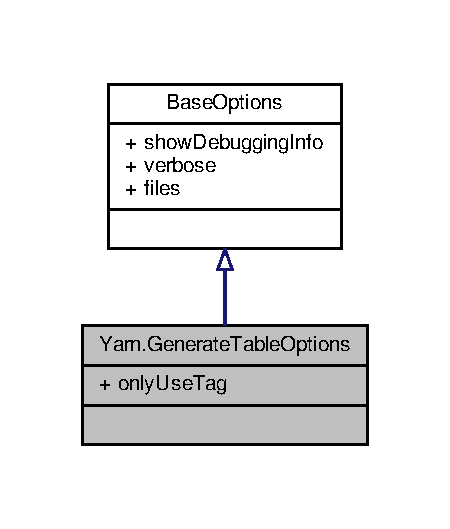
\includegraphics[width=190pt]{d9/db8/a00658}
\end{center}
\end{figure}


Collaboration diagram for Yarn.\-Compile\-Options\-:
\nopagebreak
\begin{figure}[H]
\begin{center}
\leavevmode
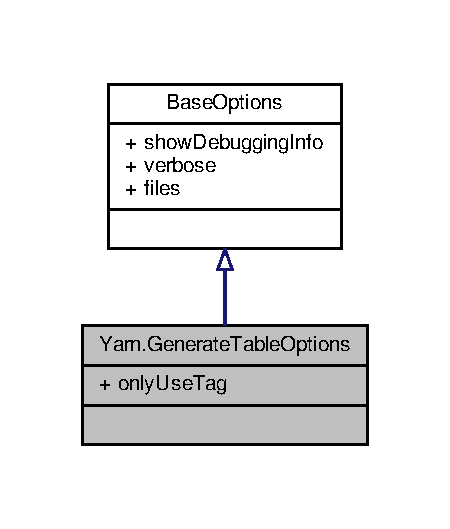
\includegraphics[width=190pt]{dc/d91/a00659}
\end{center}
\end{figure}
\subsection*{Properties}
\begin{DoxyCompactItemize}
\item 
\hyperlink{a00072_a903f18cdcc66c28ceab5a43c41fe074d}{Dialogue.\-Compiled\-Format} \hyperlink{a00035_a9904ccfb1b0ff64df415c4fc9fe6eb1c}{format}\hspace{0.3cm}{\ttfamily  \mbox{[}get, set\mbox{]}}
\item 
bool \hyperlink{a00022_a89964ea17bd19caf00cb5bff563ed01c}{show\-Debugging\-Info}\hspace{0.3cm}{\ttfamily  \mbox{[}get, set\mbox{]}}
\item 
bool \hyperlink{a00022_ada4d83d1756918f362d55f6649b82b17}{verbose}\hspace{0.3cm}{\ttfamily  \mbox{[}get, set\mbox{]}}
\item 
I\-List$<$ string $>$ \hyperlink{a00022_aa93cbb1bc1d5328e0a417012621e92d2}{files}\hspace{0.3cm}{\ttfamily  \mbox{[}get, set\mbox{]}}
\end{DoxyCompactItemize}


\subsection{Detailed Description}


\subsection{Property Documentation}
\hypertarget{a00022_aa93cbb1bc1d5328e0a417012621e92d2}{\index{Yarn\-::\-Compile\-Options@{Yarn\-::\-Compile\-Options}!files@{files}}
\index{files@{files}!Yarn::CompileOptions@{Yarn\-::\-Compile\-Options}}
\subsubsection[{files}]{\setlength{\rightskip}{0pt plus 5cm}I\-List$<$string$>$ Yarn.\-Base\-Options.\-files\hspace{0.3cm}{\ttfamily [get]}, {\ttfamily [set]}, {\ttfamily [inherited]}}}\label{a00022_aa93cbb1bc1d5328e0a417012621e92d2}
\hypertarget{a00035_a9904ccfb1b0ff64df415c4fc9fe6eb1c}{\index{Yarn\-::\-Compile\-Options@{Yarn\-::\-Compile\-Options}!format@{format}}
\index{format@{format}!Yarn::CompileOptions@{Yarn\-::\-Compile\-Options}}
\subsubsection[{format}]{\setlength{\rightskip}{0pt plus 5cm}{\bf Dialogue.\-Compiled\-Format} Yarn.\-Compile\-Options.\-format\hspace{0.3cm}{\ttfamily [get]}, {\ttfamily [set]}}}\label{a00035_a9904ccfb1b0ff64df415c4fc9fe6eb1c}
\hypertarget{a00022_a89964ea17bd19caf00cb5bff563ed01c}{\index{Yarn\-::\-Compile\-Options@{Yarn\-::\-Compile\-Options}!show\-Debugging\-Info@{show\-Debugging\-Info}}
\index{show\-Debugging\-Info@{show\-Debugging\-Info}!Yarn::CompileOptions@{Yarn\-::\-Compile\-Options}}
\subsubsection[{show\-Debugging\-Info}]{\setlength{\rightskip}{0pt plus 5cm}bool Yarn.\-Base\-Options.\-show\-Debugging\-Info\hspace{0.3cm}{\ttfamily [get]}, {\ttfamily [set]}, {\ttfamily [inherited]}}}\label{a00022_a89964ea17bd19caf00cb5bff563ed01c}
\hypertarget{a00022_ada4d83d1756918f362d55f6649b82b17}{\index{Yarn\-::\-Compile\-Options@{Yarn\-::\-Compile\-Options}!verbose@{verbose}}
\index{verbose@{verbose}!Yarn::CompileOptions@{Yarn\-::\-Compile\-Options}}
\subsubsection[{verbose}]{\setlength{\rightskip}{0pt plus 5cm}bool Yarn.\-Base\-Options.\-verbose\hspace{0.3cm}{\ttfamily [get]}, {\ttfamily [set]}, {\ttfamily [inherited]}}}\label{a00022_ada4d83d1756918f362d55f6649b82b17}


The documentation for this class was generated from the following file\-:\begin{DoxyCompactItemize}
\item 
Yarn\-Spinner\-Console/\hyperlink{a00274}{Main.\-cs}\end{DoxyCompactItemize}

\hypertarget{a00036}{\section{Yarn.\-Dialogue Class Reference}
\label{a00036}\index{Yarn.\-Dialogue@{Yarn.\-Dialogue}}
}


Collaboration diagram for Yarn.\-Dialogue\-:
\nopagebreak
\begin{figure}[H]
\begin{center}
\leavevmode
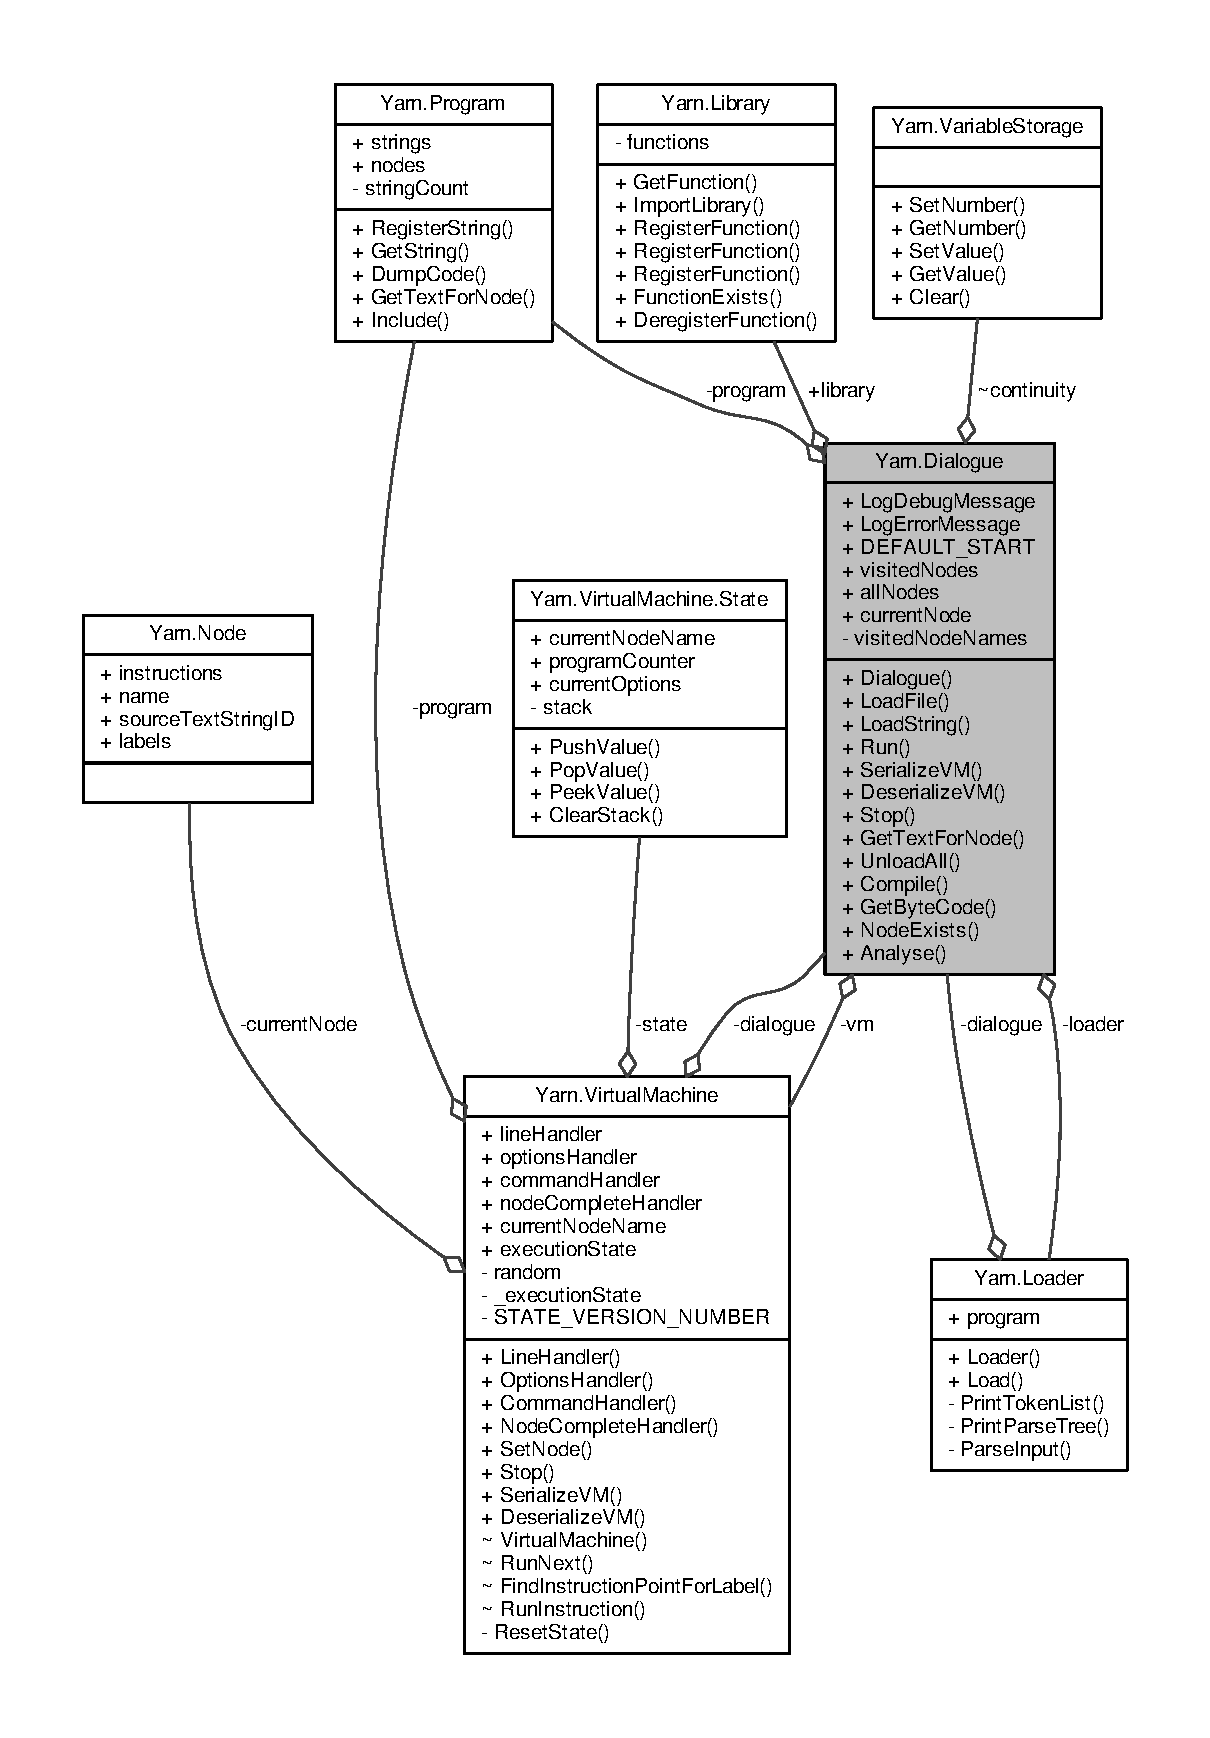
\includegraphics[width=350pt]{dc/d31/a00208}
\end{center}
\end{figure}
\subsection*{Classes}
\begin{DoxyCompactItemize}
\item 
class \hyperlink{a00027}{Command\-Result}
\item 
class \hyperlink{a00050}{Line\-Result}
\item 
class \hyperlink{a00055}{Node\-Complete\-Result}
\item 
class \hyperlink{a00060}{Option\-Set\-Result}
\item 
class \hyperlink{a00069}{Runner\-Result}
\item 
class \hyperlink{a00074}{Standard\-Library}
\end{DoxyCompactItemize}
\subsection*{Public Member Functions}
\begin{DoxyCompactItemize}
\item 
\hyperlink{a00036_a349debf4c4b8d48e3d80ff31ad380b0e}{Dialogue} (\hyperlink{a00088}{Yarn.\-Variable\-Storage} \hyperlink{a00036_ae94eaa4b03b432422f5d205fabe37ff5}{continuity})
\item 
void \hyperlink{a00036_af868f7f6928d122ca1d1857be433d92b}{Load\-File} (string file\-Name, bool show\-Tokens=false, bool show\-Parse\-Tree=false, string only\-Consider\-Node=null)
\item 
void \hyperlink{a00036_a7b66187877ec8a2bfee2298d3dd16706}{Load\-String} (string text, string file\-Name=\char`\"{}$<$input$>$\char`\"{}, bool show\-Tokens=false, bool show\-Parse\-Tree=false, string only\-Consider\-Node=null)
\item 
I\-Enumerable\\*
$<$ \hyperlink{a00069}{Yarn.\-Dialogue.\-Runner\-Result} $>$ \hyperlink{a00036_aead84ee50cb113ca45724894290ce9c2}{Run} (string start\-Node=\hyperlink{a00036_a1b643f15f734090e6a58cbf13dafd28f}{D\-E\-F\-A\-U\-L\-T\-\_\-\-S\-T\-A\-R\-T})
\item 
\hyperlink{a00026_a301aa7c866593a5b625a8fc158bbeacea27118326006d3829667a400ad23d5d98}{String} \hyperlink{a00036_aab20e7ce30fd9c2b3f19f7626be477a4}{Serialize\-V\-M} ()
\item 
void \hyperlink{a00036_aaa680fc471c1d78fd75ed3bde9b491e3}{Deserialize\-V\-M} (string encoded)
\item 
void \hyperlink{a00036_a7a6cabe5612fdcdc4619460431f85112}{Stop} ()
\item 
string \hyperlink{a00036_a594641914a2b59cc5231645273d18e82}{Get\-Text\-For\-Node} (string node\-Name)
\item 
void \hyperlink{a00036_a7acfe32f91b36ee812059f2ad3011133}{Unload\-All} (bool clear\-Visited\-Nodes=true)
\item 
\hyperlink{a00026_a301aa7c866593a5b625a8fc158bbeacea27118326006d3829667a400ad23d5d98}{String} \hyperlink{a00036_a7a8a3a461011172f5624da3a8ffa875f}{Compile} ()
\item 
\hyperlink{a00026_a301aa7c866593a5b625a8fc158bbeacea27118326006d3829667a400ad23d5d98}{String} \hyperlink{a00036_aade6c069db8f01572060d25a963d2a14}{Get\-Byte\-Code} ()
\item 
bool \hyperlink{a00036_a93bb76a1f9a4058f225ff4cee97483c6}{Node\-Exists} (string node\-Name)
\item 
void \hyperlink{a00036_a6b67b239f50c062160666e54592c433f}{Analyse} (\hyperlink{a00031}{Analysis.\-Context} context)
\end{DoxyCompactItemize}
\subsection*{Public Attributes}
\begin{DoxyCompactItemize}
\item 
\hyperlink{a00026_a1e50031b945a3a2afafee6f590730568}{Logger} \hyperlink{a00036_a381f48bb0fbb294f8cf44ca57f11be31}{Log\-Debug\-Message}
\item 
\hyperlink{a00026_a1e50031b945a3a2afafee6f590730568}{Logger} \hyperlink{a00036_a9801e83dd044d6498fdf6ebcc6bec5ac}{Log\-Error\-Message}
\item 
const string \hyperlink{a00036_a1b643f15f734090e6a58cbf13dafd28f}{D\-E\-F\-A\-U\-L\-T\-\_\-\-S\-T\-A\-R\-T} = \char`\"{}Start\char`\"{}
\item 
\hyperlink{a00049}{Library} \hyperlink{a00036_ae660d4cfb6e296358d2f61d8ee74c66a}{library}
\end{DoxyCompactItemize}
\subsection*{Package Attributes}
\begin{DoxyCompactItemize}
\item 
\hyperlink{a00088}{Variable\-Storage} \hyperlink{a00036_ae94eaa4b03b432422f5d205fabe37ff5}{continuity}
\end{DoxyCompactItemize}
\subsection*{Properties}
\begin{DoxyCompactItemize}
\item 
I\-Enumerable$<$ string $>$ \hyperlink{a00036_ac5661051e0b7f44527fe526c7766dbbf}{visited\-Nodes}\hspace{0.3cm}{\ttfamily  \mbox{[}get\mbox{]}}
\item 
I\-Enumerable$<$ string $>$ \hyperlink{a00036_a0ee573e3d072bccf98ba1d975612d42c}{all\-Nodes}\hspace{0.3cm}{\ttfamily  \mbox{[}get\mbox{]}}
\item 
string \hyperlink{a00036_af368b5c342d585dc6953876c5965ccc8}{current\-Node}\hspace{0.3cm}{\ttfamily  \mbox{[}get\mbox{]}}
\end{DoxyCompactItemize}
\subsection*{Private Attributes}
\begin{DoxyCompactItemize}
\item 
\hyperlink{a00051}{Loader} \hyperlink{a00036_a98bbe0ac2ccadeeeb7e05e3e6e19f2e0}{loader}
\item 
\hyperlink{a00067}{Program} \hyperlink{a00036_a0a1cca92325f430425d784d416cb5c2b}{program}
\item 
Hash\-Set$<$ \hyperlink{a00026_a301aa7c866593a5b625a8fc158bbeacea27118326006d3829667a400ad23d5d98}{String} $>$ \hyperlink{a00036_a41fb2e23171610197d66d2c01d4023f6}{visited\-Node\-Names} = new Hash\-Set$<$string$>$()
\item 
\hyperlink{a00072}{Virtual\-Machine} \hyperlink{a00036_a8c1319357a9df6cff051328fb33224c7}{vm}
\end{DoxyCompactItemize}


\subsection{Detailed Description}


\subsection{Constructor \& Destructor Documentation}
\hypertarget{a00036_a349debf4c4b8d48e3d80ff31ad380b0e}{\index{Yarn\-::\-Dialogue@{Yarn\-::\-Dialogue}!Dialogue@{Dialogue}}
\index{Dialogue@{Dialogue}!Yarn::Dialogue@{Yarn\-::\-Dialogue}}
\subsubsection[{Dialogue}]{\setlength{\rightskip}{0pt plus 5cm}Yarn.\-Dialogue.\-Dialogue (
\begin{DoxyParamCaption}
\item[{{\bf Yarn.\-Variable\-Storage}}]{continuity}
\end{DoxyParamCaption}
)}}\label{a00036_a349debf4c4b8d48e3d80ff31ad380b0e}

\begin{DoxyCode}
160                                                          \{
161             this.continuity = \hyperlink{a00036_ae94eaa4b03b432422f5d205fabe37ff5}{continuity};
162             \hyperlink{a00036_a98bbe0ac2ccadeeeb7e05e3e6e19f2e0}{loader} = \textcolor{keyword}{new} Loader (\textcolor{keyword}{this});
163             \hyperlink{a00036_ae660d4cfb6e296358d2f61d8ee74c66a}{library} = \textcolor{keyword}{new} Library ();
164 
165             library.ImportLibrary (\textcolor{keyword}{new} StandardLibrary ());
166 
167             \textcolor{comment}{// Register the "visited" function, which returns true if we've visited}
168             \textcolor{comment}{// a node previously (nodes are marked as visited when we leave them)}
169             library.RegisterFunction (\textcolor{stringliteral}{"visited"}, 1, delegate(Yarn.Value[] parameters) \{
170                 var name = parameters[0].AsString;
171                 \textcolor{keywordflow}{return} visitedNodeNames.Contains(name);
172             \});
173 
174         \}
\end{DoxyCode}


\subsection{Member Function Documentation}
\hypertarget{a00036_a6b67b239f50c062160666e54592c433f}{\index{Yarn\-::\-Dialogue@{Yarn\-::\-Dialogue}!Analyse@{Analyse}}
\index{Analyse@{Analyse}!Yarn::Dialogue@{Yarn\-::\-Dialogue}}
\subsubsection[{Analyse}]{\setlength{\rightskip}{0pt plus 5cm}void Yarn.\-Dialogue.\-Analyse (
\begin{DoxyParamCaption}
\item[{{\bf Analysis.\-Context}}]{context}
\end{DoxyParamCaption}
)}}\label{a00036_a6b67b239f50c062160666e54592c433f}

\begin{DoxyCode}
353                                                       \{
354 
355             context.AddProgramToAnalysis (this.program);
356 
357         \}
\end{DoxyCode}
\hypertarget{a00036_a7a8a3a461011172f5624da3a8ffa875f}{\index{Yarn\-::\-Dialogue@{Yarn\-::\-Dialogue}!Compile@{Compile}}
\index{Compile@{Compile}!Yarn::Dialogue@{Yarn\-::\-Dialogue}}
\subsubsection[{Compile}]{\setlength{\rightskip}{0pt plus 5cm}{\bf String} Yarn.\-Dialogue.\-Compile (
\begin{DoxyParamCaption}
{}
\end{DoxyParamCaption}
)}}\label{a00036_a7a8a3a461011172f5624da3a8ffa875f}

\begin{DoxyCode}
323                                 \{
324             \textcolor{keywordflow}{return} program.DumpCode (\hyperlink{a00036_ae660d4cfb6e296358d2f61d8ee74c66a}{library});
325         \}
\end{DoxyCode}
\hypertarget{a00036_aaa680fc471c1d78fd75ed3bde9b491e3}{\index{Yarn\-::\-Dialogue@{Yarn\-::\-Dialogue}!Deserialize\-V\-M@{Deserialize\-V\-M}}
\index{Deserialize\-V\-M@{Deserialize\-V\-M}!Yarn::Dialogue@{Yarn\-::\-Dialogue}}
\subsubsection[{Deserialize\-V\-M}]{\setlength{\rightskip}{0pt plus 5cm}void Yarn.\-Dialogue.\-Deserialize\-V\-M (
\begin{DoxyParamCaption}
\item[{string}]{encoded}
\end{DoxyParamCaption}
)}}\label{a00036_aaa680fc471c1d78fd75ed3bde9b491e3}

\begin{DoxyCode}
269         \{
270             vm.DeserializeVM(encoded);
271         \}
\end{DoxyCode}
\hypertarget{a00036_aade6c069db8f01572060d25a963d2a14}{\index{Yarn\-::\-Dialogue@{Yarn\-::\-Dialogue}!Get\-Byte\-Code@{Get\-Byte\-Code}}
\index{Get\-Byte\-Code@{Get\-Byte\-Code}!Yarn::Dialogue@{Yarn\-::\-Dialogue}}
\subsubsection[{Get\-Byte\-Code}]{\setlength{\rightskip}{0pt plus 5cm}{\bf String} Yarn.\-Dialogue.\-Get\-Byte\-Code (
\begin{DoxyParamCaption}
{}
\end{DoxyParamCaption}
)}}\label{a00036_aade6c069db8f01572060d25a963d2a14}

\begin{DoxyCode}
327                                     \{
328             \textcolor{keywordflow}{return} program.DumpCode (\hyperlink{a00036_ae660d4cfb6e296358d2f61d8ee74c66a}{library});
329         \}
\end{DoxyCode}
\hypertarget{a00036_a594641914a2b59cc5231645273d18e82}{\index{Yarn\-::\-Dialogue@{Yarn\-::\-Dialogue}!Get\-Text\-For\-Node@{Get\-Text\-For\-Node}}
\index{Get\-Text\-For\-Node@{Get\-Text\-For\-Node}!Yarn::Dialogue@{Yarn\-::\-Dialogue}}
\subsubsection[{Get\-Text\-For\-Node}]{\setlength{\rightskip}{0pt plus 5cm}string Yarn.\-Dialogue.\-Get\-Text\-For\-Node (
\begin{DoxyParamCaption}
\item[{string}]{node\-Name}
\end{DoxyParamCaption}
)}}\label{a00036_a594641914a2b59cc5231645273d18e82}

\begin{DoxyCode}
301                                                       \{
302             \textcolor{keywordflow}{if} (\hyperlink{a00036_a0a1cca92325f430425d784d416cb5c2b}{program}.\hyperlink{a00067_a3f4928a577c88263ad016be259b175c4}{nodes}.Count == 0) \{
303                 \hyperlink{a00036_a9801e83dd044d6498fdf6ebcc6bec5ac}{LogErrorMessage} (\textcolor{stringliteral}{"No nodes are loaded!"});
304                 \textcolor{keywordflow}{return} null;
305             \} \textcolor{keywordflow}{else} \textcolor{keywordflow}{if} (\hyperlink{a00036_a0a1cca92325f430425d784d416cb5c2b}{program}.\hyperlink{a00067_a3f4928a577c88263ad016be259b175c4}{nodes}.ContainsKey(nodeName)) \{
306                 \textcolor{keywordflow}{return} program.GetTextForNode (nodeName);
307             \} \textcolor{keywordflow}{else} \{
308                 \hyperlink{a00036_a9801e83dd044d6498fdf6ebcc6bec5ac}{LogErrorMessage} (\textcolor{stringliteral}{"No node named "} + nodeName);
309                 \textcolor{keywordflow}{return} null;
310             \}
311         \}
\end{DoxyCode}
\hypertarget{a00036_af868f7f6928d122ca1d1857be433d92b}{\index{Yarn\-::\-Dialogue@{Yarn\-::\-Dialogue}!Load\-File@{Load\-File}}
\index{Load\-File@{Load\-File}!Yarn::Dialogue@{Yarn\-::\-Dialogue}}
\subsubsection[{Load\-File}]{\setlength{\rightskip}{0pt plus 5cm}void Yarn.\-Dialogue.\-Load\-File (
\begin{DoxyParamCaption}
\item[{string}]{file\-Name, }
\item[{bool}]{show\-Tokens = {\ttfamily false}, }
\item[{bool}]{show\-Parse\-Tree = {\ttfamily false}, }
\item[{string}]{only\-Consider\-Node = {\ttfamily null}}
\end{DoxyParamCaption}
)}}\label{a00036_af868f7f6928d122ca1d1857be433d92b}

\begin{DoxyCode}
177                                                                                                            
                            \{
178             System.IO.StreamReader reader = \textcolor{keyword}{new} System.IO.StreamReader(fileName);
179             \textcolor{keywordtype}{string} inputString = reader.ReadToEnd ();
180             reader.Close ();
181 
182             \hyperlink{a00036_a7b66187877ec8a2bfee2298d3dd16706}{LoadString} (inputString, fileName, showTokens, showParseTree, onlyConsiderNode);
183 
184         \}
\end{DoxyCode}
\hypertarget{a00036_a7b66187877ec8a2bfee2298d3dd16706}{\index{Yarn\-::\-Dialogue@{Yarn\-::\-Dialogue}!Load\-String@{Load\-String}}
\index{Load\-String@{Load\-String}!Yarn::Dialogue@{Yarn\-::\-Dialogue}}
\subsubsection[{Load\-String}]{\setlength{\rightskip}{0pt plus 5cm}void Yarn.\-Dialogue.\-Load\-String (
\begin{DoxyParamCaption}
\item[{string}]{text, }
\item[{string}]{file\-Name = {\ttfamily \char`\"{}$<$input$>$\char`\"{}}, }
\item[{bool}]{show\-Tokens = {\ttfamily false}, }
\item[{bool}]{show\-Parse\-Tree = {\ttfamily false}, }
\item[{string}]{only\-Consider\-Node = {\ttfamily null}}
\end{DoxyParamCaption}
)}}\label{a00036_a7b66187877ec8a2bfee2298d3dd16706}

\begin{DoxyCode}
187                                                                                                            
                                                 \{
188 
189             \textcolor{keywordflow}{if} (\hyperlink{a00036_a381f48bb0fbb294f8cf44ca57f11be31}{LogDebugMessage} == null) \{
190                 \textcolor{keywordflow}{throw} \textcolor{keyword}{new} YarnException (\textcolor{stringliteral}{"LogDebugMessage must be set before loading"});
191             \}
192 
193             \textcolor{keywordflow}{if} (\hyperlink{a00036_a9801e83dd044d6498fdf6ebcc6bec5ac}{LogErrorMessage} == null) \{
194                 \textcolor{keywordflow}{throw} \textcolor{keyword}{new} YarnException (\textcolor{stringliteral}{"LogErrorMessage must be set before loading"});
195             \}
196 
197             \hyperlink{a00036_a0a1cca92325f430425d784d416cb5c2b}{program} = loader.Load(text, \hyperlink{a00036_ae660d4cfb6e296358d2f61d8ee74c66a}{library}, fileName, \hyperlink{a00036_a0a1cca92325f430425d784d416cb5c2b}{program}, showTokens, 
      showParseTree, onlyConsiderNode);
198 
199         \}
\end{DoxyCode}
\hypertarget{a00036_a93bb76a1f9a4058f225ff4cee97483c6}{\index{Yarn\-::\-Dialogue@{Yarn\-::\-Dialogue}!Node\-Exists@{Node\-Exists}}
\index{Node\-Exists@{Node\-Exists}!Yarn::Dialogue@{Yarn\-::\-Dialogue}}
\subsubsection[{Node\-Exists}]{\setlength{\rightskip}{0pt plus 5cm}bool Yarn.\-Dialogue.\-Node\-Exists (
\begin{DoxyParamCaption}
\item[{string}]{node\-Name}
\end{DoxyParamCaption}
)}}\label{a00036_a93bb76a1f9a4058f225ff4cee97483c6}

\begin{DoxyCode}
331                                                 \{
332             \textcolor{keywordflow}{if} (\hyperlink{a00036_a0a1cca92325f430425d784d416cb5c2b}{program} == null) \{
333 
334                 \textcolor{keywordflow}{if} (\hyperlink{a00036_a0a1cca92325f430425d784d416cb5c2b}{program}.\hyperlink{a00067_a3f4928a577c88263ad016be259b175c4}{nodes}.Count > 0) \{
335                     \hyperlink{a00036_a381f48bb0fbb294f8cf44ca57f11be31}{LogDebugMessage} (\textcolor{stringliteral}{"Called NodeExists, but the program hasn't been
       compiled yet."} +
336                     \textcolor{stringliteral}{"Nodes have been loaded, so I'm going to compile them."});
337 
338                     \textcolor{keywordflow}{if} (\hyperlink{a00036_a0a1cca92325f430425d784d416cb5c2b}{program} == null) \{
339                         \textcolor{keywordflow}{return} \textcolor{keyword}{false};
340                     \}
341                 \} \textcolor{keywordflow}{else} \{
342                     \hyperlink{a00036_a9801e83dd044d6498fdf6ebcc6bec5ac}{LogErrorMessage} (\textcolor{stringliteral}{"Tried to call NodeExists, but no nodes have been
       compiled!"});
343                     \textcolor{keywordflow}{return} \textcolor{keyword}{false};
344                 \}
345             \}
346             \textcolor{keywordflow}{if} (\hyperlink{a00036_a0a1cca92325f430425d784d416cb5c2b}{program}.\hyperlink{a00067_a3f4928a577c88263ad016be259b175c4}{nodes} == null || \hyperlink{a00036_a0a1cca92325f430425d784d416cb5c2b}{program}.\hyperlink{a00067_a3f4928a577c88263ad016be259b175c4}{nodes}.Count == 0) \{
347                 \hyperlink{a00036_a381f48bb0fbb294f8cf44ca57f11be31}{LogDebugMessage} (\textcolor{stringliteral}{"Called NodeExists, but there are zero nodes. This may be
       an error."});
348                 \textcolor{keywordflow}{return} \textcolor{keyword}{false};
349             \}
350             \textcolor{keywordflow}{return} program.nodes.ContainsKey(nodeName);
351         \}
\end{DoxyCode}
\hypertarget{a00036_aead84ee50cb113ca45724894290ce9c2}{\index{Yarn\-::\-Dialogue@{Yarn\-::\-Dialogue}!Run@{Run}}
\index{Run@{Run}!Yarn::Dialogue@{Yarn\-::\-Dialogue}}
\subsubsection[{Run}]{\setlength{\rightskip}{0pt plus 5cm}I\-Enumerable$<${\bf Yarn.\-Dialogue.\-Runner\-Result}$>$ Yarn.\-Dialogue.\-Run (
\begin{DoxyParamCaption}
\item[{string}]{start\-Node = {\ttfamily {\bf D\-E\-F\-A\-U\-L\-T\-\_\-\-S\-T\-A\-R\-T}}}
\end{DoxyParamCaption}
)}}\label{a00036_aead84ee50cb113ca45724894290ce9c2}

\begin{DoxyCode}
205                                                                                              \{
206 
207 
208             \textcolor{keywordflow}{if} (\hyperlink{a00036_a381f48bb0fbb294f8cf44ca57f11be31}{LogDebugMessage} == null) \{
209                 \textcolor{keywordflow}{throw} \textcolor{keyword}{new} YarnException (\textcolor{stringliteral}{"LogDebugMessage must be set before running"});
210             \}
211 
212             \textcolor{keywordflow}{if} (\hyperlink{a00036_a9801e83dd044d6498fdf6ebcc6bec5ac}{LogErrorMessage} == null) \{
213                 \textcolor{keywordflow}{throw} \textcolor{keyword}{new} YarnException (\textcolor{stringliteral}{"LogErrorMessage must be set before running"});
214             \}
215 
216             \textcolor{keywordflow}{if} (\hyperlink{a00036_a0a1cca92325f430425d784d416cb5c2b}{program} == null) \{
217                 \hyperlink{a00036_a9801e83dd044d6498fdf6ebcc6bec5ac}{LogErrorMessage} (\textcolor{stringliteral}{"Dialogue.Run was called, but no program was loaded.
       Stopping."});
218                 yield \textcolor{keywordflow}{break};
219             \}
220 
221             \hyperlink{a00036_a8c1319357a9df6cff051328fb33224c7}{vm} = \textcolor{keyword}{new} VirtualMachine (\textcolor{keyword}{this}, \hyperlink{a00036_a0a1cca92325f430425d784d416cb5c2b}{program});
222 
223             RunnerResult latestResult;
224 
225             vm.lineHandler = delegate(LineResult result) \{
226                 latestResult = result;
227             \};
228 
229             vm.commandHandler = delegate(CommandResult result) \{
230                 \textcolor{comment}{// Is it the special custom command "<<stop>>"?}
231                 \textcolor{keywordflow}{if} (result is CommandResult && (result as CommandResult).command.text == \textcolor{stringliteral}{"stop"}) \{
232                     vm.Stop();
233                 \}
234                 latestResult = result;
235             \};
236 
237             vm.nodeCompleteHandler = delegate(NodeCompleteResult result) \{
238                 visitedNodeNames.Add (vm.currentNodeName);
239                 latestResult = result;
240             \};
241 
242             vm.optionsHandler = delegate(OptionSetResult result) \{
243                 latestResult = result;
244             \};
245 
246             \textcolor{keywordflow}{if} (\hyperlink{a00036_a8c1319357a9df6cff051328fb33224c7}{vm}.\hyperlink{a00072_a6364593ea1115d65e34b343422cfbbbd}{SetNode} (startNode) == \textcolor{keyword}{false}) \{
247                 yield \textcolor{keywordflow}{break};
248             \}
249 
250             \textcolor{comment}{// Run until the program stops, pausing to yield important}
251             \textcolor{comment}{// results}
252             \textcolor{keywordflow}{do} \{
253 
254                 latestResult = null;
255                 vm.RunNext ();
256                 \textcolor{keywordflow}{if} (latestResult != null)
257                     yield \textcolor{keywordflow}{return} latestResult;
258 
259             \} \textcolor{keywordflow}{while} (\hyperlink{a00036_a8c1319357a9df6cff051328fb33224c7}{vm}.\hyperlink{a00072_a66491da06023dabfb63d09e6ccbba74f}{executionState} != VirtualMachine.ExecutionState.Stopped);
260 
261         \}
\end{DoxyCode}
\hypertarget{a00036_aab20e7ce30fd9c2b3f19f7626be477a4}{\index{Yarn\-::\-Dialogue@{Yarn\-::\-Dialogue}!Serialize\-V\-M@{Serialize\-V\-M}}
\index{Serialize\-V\-M@{Serialize\-V\-M}!Yarn::Dialogue@{Yarn\-::\-Dialogue}}
\subsubsection[{Serialize\-V\-M}]{\setlength{\rightskip}{0pt plus 5cm}{\bf String} Yarn.\-Dialogue.\-Serialize\-V\-M (
\begin{DoxyParamCaption}
{}
\end{DoxyParamCaption}
)}}\label{a00036_aab20e7ce30fd9c2b3f19f7626be477a4}

\begin{DoxyCode}
264         \{
265             \textcolor{keywordflow}{return} vm.SerializeVM();
266         \}
\end{DoxyCode}
\hypertarget{a00036_a7a6cabe5612fdcdc4619460431f85112}{\index{Yarn\-::\-Dialogue@{Yarn\-::\-Dialogue}!Stop@{Stop}}
\index{Stop@{Stop}!Yarn::Dialogue@{Yarn\-::\-Dialogue}}
\subsubsection[{Stop}]{\setlength{\rightskip}{0pt plus 5cm}void Yarn.\-Dialogue.\-Stop (
\begin{DoxyParamCaption}
{}
\end{DoxyParamCaption}
)}}\label{a00036_a7a6cabe5612fdcdc4619460431f85112}

\begin{DoxyCode}
273                            \{
274             \textcolor{keywordflow}{if} (\hyperlink{a00036_a8c1319357a9df6cff051328fb33224c7}{vm} != null)
275                 vm.Stop();
276         \}
\end{DoxyCode}
\hypertarget{a00036_a7acfe32f91b36ee812059f2ad3011133}{\index{Yarn\-::\-Dialogue@{Yarn\-::\-Dialogue}!Unload\-All@{Unload\-All}}
\index{Unload\-All@{Unload\-All}!Yarn::Dialogue@{Yarn\-::\-Dialogue}}
\subsubsection[{Unload\-All}]{\setlength{\rightskip}{0pt plus 5cm}void Yarn.\-Dialogue.\-Unload\-All (
\begin{DoxyParamCaption}
\item[{bool}]{clear\-Visited\-Nodes = {\ttfamily true}}
\end{DoxyParamCaption}
)}}\label{a00036_a7acfe32f91b36ee812059f2ad3011133}

\begin{DoxyCode}
314                                                              \{
315             \textcolor{keywordflow}{if} (clearVisitedNodes)
316                 visitedNodeNames.Clear();
317 
318             \hyperlink{a00036_a0a1cca92325f430425d784d416cb5c2b}{program} = null;
319 
320         \}
\end{DoxyCode}


\subsection{Member Data Documentation}
\hypertarget{a00036_ae94eaa4b03b432422f5d205fabe37ff5}{\index{Yarn\-::\-Dialogue@{Yarn\-::\-Dialogue}!continuity@{continuity}}
\index{continuity@{continuity}!Yarn::Dialogue@{Yarn\-::\-Dialogue}}
\subsubsection[{continuity}]{\setlength{\rightskip}{0pt plus 5cm}{\bf Variable\-Storage} Yarn.\-Dialogue.\-continuity\hspace{0.3cm}{\ttfamily [package]}}}\label{a00036_ae94eaa4b03b432422f5d205fabe37ff5}
\hypertarget{a00036_a1b643f15f734090e6a58cbf13dafd28f}{\index{Yarn\-::\-Dialogue@{Yarn\-::\-Dialogue}!D\-E\-F\-A\-U\-L\-T\-\_\-\-S\-T\-A\-R\-T@{D\-E\-F\-A\-U\-L\-T\-\_\-\-S\-T\-A\-R\-T}}
\index{D\-E\-F\-A\-U\-L\-T\-\_\-\-S\-T\-A\-R\-T@{D\-E\-F\-A\-U\-L\-T\-\_\-\-S\-T\-A\-R\-T}!Yarn::Dialogue@{Yarn\-::\-Dialogue}}
\subsubsection[{D\-E\-F\-A\-U\-L\-T\-\_\-\-S\-T\-A\-R\-T}]{\setlength{\rightskip}{0pt plus 5cm}const string Yarn.\-Dialogue.\-D\-E\-F\-A\-U\-L\-T\-\_\-\-S\-T\-A\-R\-T = \char`\"{}Start\char`\"{}}}\label{a00036_a1b643f15f734090e6a58cbf13dafd28f}
\hypertarget{a00036_ae660d4cfb6e296358d2f61d8ee74c66a}{\index{Yarn\-::\-Dialogue@{Yarn\-::\-Dialogue}!library@{library}}
\index{library@{library}!Yarn::Dialogue@{Yarn\-::\-Dialogue}}
\subsubsection[{library}]{\setlength{\rightskip}{0pt plus 5cm}{\bf Library} Yarn.\-Dialogue.\-library}}\label{a00036_ae660d4cfb6e296358d2f61d8ee74c66a}
\hypertarget{a00036_a98bbe0ac2ccadeeeb7e05e3e6e19f2e0}{\index{Yarn\-::\-Dialogue@{Yarn\-::\-Dialogue}!loader@{loader}}
\index{loader@{loader}!Yarn::Dialogue@{Yarn\-::\-Dialogue}}
\subsubsection[{loader}]{\setlength{\rightskip}{0pt plus 5cm}{\bf Loader} Yarn.\-Dialogue.\-loader\hspace{0.3cm}{\ttfamily [private]}}}\label{a00036_a98bbe0ac2ccadeeeb7e05e3e6e19f2e0}
\hypertarget{a00036_a381f48bb0fbb294f8cf44ca57f11be31}{\index{Yarn\-::\-Dialogue@{Yarn\-::\-Dialogue}!Log\-Debug\-Message@{Log\-Debug\-Message}}
\index{Log\-Debug\-Message@{Log\-Debug\-Message}!Yarn::Dialogue@{Yarn\-::\-Dialogue}}
\subsubsection[{Log\-Debug\-Message}]{\setlength{\rightskip}{0pt plus 5cm}{\bf Logger} Yarn.\-Dialogue.\-Log\-Debug\-Message}}\label{a00036_a381f48bb0fbb294f8cf44ca57f11be31}
\hypertarget{a00036_a9801e83dd044d6498fdf6ebcc6bec5ac}{\index{Yarn\-::\-Dialogue@{Yarn\-::\-Dialogue}!Log\-Error\-Message@{Log\-Error\-Message}}
\index{Log\-Error\-Message@{Log\-Error\-Message}!Yarn::Dialogue@{Yarn\-::\-Dialogue}}
\subsubsection[{Log\-Error\-Message}]{\setlength{\rightskip}{0pt plus 5cm}{\bf Logger} Yarn.\-Dialogue.\-Log\-Error\-Message}}\label{a00036_a9801e83dd044d6498fdf6ebcc6bec5ac}
\hypertarget{a00036_a0a1cca92325f430425d784d416cb5c2b}{\index{Yarn\-::\-Dialogue@{Yarn\-::\-Dialogue}!program@{program}}
\index{program@{program}!Yarn::Dialogue@{Yarn\-::\-Dialogue}}
\subsubsection[{program}]{\setlength{\rightskip}{0pt plus 5cm}{\bf Program} Yarn.\-Dialogue.\-program\hspace{0.3cm}{\ttfamily [private]}}}\label{a00036_a0a1cca92325f430425d784d416cb5c2b}
\hypertarget{a00036_a41fb2e23171610197d66d2c01d4023f6}{\index{Yarn\-::\-Dialogue@{Yarn\-::\-Dialogue}!visited\-Node\-Names@{visited\-Node\-Names}}
\index{visited\-Node\-Names@{visited\-Node\-Names}!Yarn::Dialogue@{Yarn\-::\-Dialogue}}
\subsubsection[{visited\-Node\-Names}]{\setlength{\rightskip}{0pt plus 5cm}Hash\-Set$<${\bf String}$>$ Yarn.\-Dialogue.\-visited\-Node\-Names = new Hash\-Set$<$string$>$()\hspace{0.3cm}{\ttfamily [private]}}}\label{a00036_a41fb2e23171610197d66d2c01d4023f6}
\hypertarget{a00036_a8c1319357a9df6cff051328fb33224c7}{\index{Yarn\-::\-Dialogue@{Yarn\-::\-Dialogue}!vm@{vm}}
\index{vm@{vm}!Yarn::Dialogue@{Yarn\-::\-Dialogue}}
\subsubsection[{vm}]{\setlength{\rightskip}{0pt plus 5cm}{\bf Virtual\-Machine} Yarn.\-Dialogue.\-vm\hspace{0.3cm}{\ttfamily [private]}}}\label{a00036_a8c1319357a9df6cff051328fb33224c7}


\subsection{Property Documentation}
\hypertarget{a00036_a0ee573e3d072bccf98ba1d975612d42c}{\index{Yarn\-::\-Dialogue@{Yarn\-::\-Dialogue}!all\-Nodes@{all\-Nodes}}
\index{all\-Nodes@{all\-Nodes}!Yarn::Dialogue@{Yarn\-::\-Dialogue}}
\subsubsection[{all\-Nodes}]{\setlength{\rightskip}{0pt plus 5cm}I\-Enumerable$<$string$>$ Yarn.\-Dialogue.\-all\-Nodes\hspace{0.3cm}{\ttfamily [get]}}}\label{a00036_a0ee573e3d072bccf98ba1d975612d42c}
\hypertarget{a00036_af368b5c342d585dc6953876c5965ccc8}{\index{Yarn\-::\-Dialogue@{Yarn\-::\-Dialogue}!current\-Node@{current\-Node}}
\index{current\-Node@{current\-Node}!Yarn::Dialogue@{Yarn\-::\-Dialogue}}
\subsubsection[{current\-Node}]{\setlength{\rightskip}{0pt plus 5cm}string Yarn.\-Dialogue.\-current\-Node\hspace{0.3cm}{\ttfamily [get]}}}\label{a00036_af368b5c342d585dc6953876c5965ccc8}
\hypertarget{a00036_ac5661051e0b7f44527fe526c7766dbbf}{\index{Yarn\-::\-Dialogue@{Yarn\-::\-Dialogue}!visited\-Nodes@{visited\-Nodes}}
\index{visited\-Nodes@{visited\-Nodes}!Yarn::Dialogue@{Yarn\-::\-Dialogue}}
\subsubsection[{visited\-Nodes}]{\setlength{\rightskip}{0pt plus 5cm}I\-Enumerable$<$string$>$ Yarn.\-Dialogue.\-visited\-Nodes\hspace{0.3cm}{\ttfamily [get]}}}\label{a00036_ac5661051e0b7f44527fe526c7766dbbf}


The documentation for this class was generated from the following file\-:\begin{DoxyCompactItemize}
\item 
Yarn\-Spinner/\hyperlink{a00117}{Dialogue.\-cs}\end{DoxyCompactItemize}

\hypertarget{a00037}{\section{Yarn.\-Add\-Labels\-Options Class Reference}
\label{a00037}\index{Yarn.\-Add\-Labels\-Options@{Yarn.\-Add\-Labels\-Options}}
}


Inheritance diagram for Yarn.\-Add\-Labels\-Options\-:
\nopagebreak
\begin{figure}[H]
\begin{center}
\leavevmode
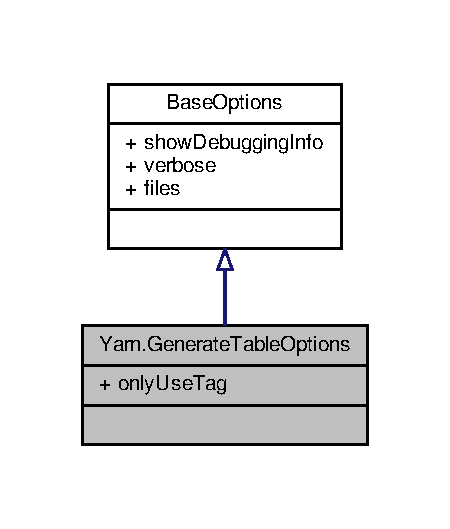
\includegraphics[width=198pt]{a00750}
\end{center}
\end{figure}


Collaboration diagram for Yarn.\-Add\-Labels\-Options\-:
\nopagebreak
\begin{figure}[H]
\begin{center}
\leavevmode
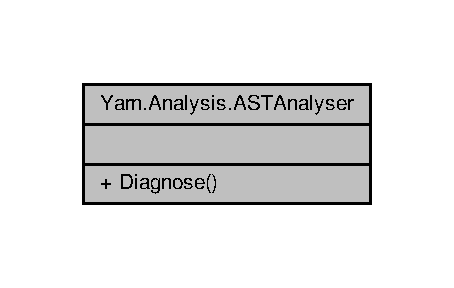
\includegraphics[width=198pt]{a00751}
\end{center}
\end{figure}
\subsection*{Properties}
\begin{DoxyCompactItemize}
\item 
bool \hyperlink{a00037_a5dc9d9db767738237e988f95fc0330f4}{dry\-Run}\hspace{0.3cm}{\ttfamily  \mbox{[}get, set\mbox{]}}
\item 
string \hyperlink{a00037_ab6162338f9606a836f3101fe0e228249}{only\-Use\-Tag}\hspace{0.3cm}{\ttfamily  \mbox{[}get, set\mbox{]}}
\item 
bool \hyperlink{a00041_a89964ea17bd19caf00cb5bff563ed01c}{show\-Debugging\-Info}\hspace{0.3cm}{\ttfamily  \mbox{[}get, set\mbox{]}}
\item 
bool \hyperlink{a00041_ada4d83d1756918f362d55f6649b82b17}{verbose}\hspace{0.3cm}{\ttfamily  \mbox{[}get, set\mbox{]}}
\item 
I\-List$<$ string $>$ \hyperlink{a00041_aa93cbb1bc1d5328e0a417012621e92d2}{files}\hspace{0.3cm}{\ttfamily  \mbox{[}get, set\mbox{]}}
\end{DoxyCompactItemize}


\subsection{Detailed Description}


Definition at line 118 of file Main.\-cs.



\subsection{Property Documentation}
\hypertarget{a00037_a5dc9d9db767738237e988f95fc0330f4}{\index{Yarn\-::\-Add\-Labels\-Options@{Yarn\-::\-Add\-Labels\-Options}!dry\-Run@{dry\-Run}}
\index{dry\-Run@{dry\-Run}!Yarn::AddLabelsOptions@{Yarn\-::\-Add\-Labels\-Options}}
\subsubsection[{dry\-Run}]{\setlength{\rightskip}{0pt plus 5cm}bool Yarn.\-Add\-Labels\-Options.\-dry\-Run\hspace{0.3cm}{\ttfamily [get]}, {\ttfamily [set]}}}\label{a00037_a5dc9d9db767738237e988f95fc0330f4}


Definition at line 122 of file Main.\-cs.

\hypertarget{a00041_aa93cbb1bc1d5328e0a417012621e92d2}{\index{Yarn\-::\-Add\-Labels\-Options@{Yarn\-::\-Add\-Labels\-Options}!files@{files}}
\index{files@{files}!Yarn::AddLabelsOptions@{Yarn\-::\-Add\-Labels\-Options}}
\subsubsection[{files}]{\setlength{\rightskip}{0pt plus 5cm}I\-List$<$string$>$ Yarn.\-Base\-Options.\-files\hspace{0.3cm}{\ttfamily [get]}, {\ttfamily [set]}, {\ttfamily [inherited]}}}\label{a00041_aa93cbb1bc1d5328e0a417012621e92d2}


Definition at line 49 of file Main.\-cs.



Referenced by Yarn.\-Yarn\-Spinner\-Console.\-Run(), and Yarn.\-Yarn\-Spinner\-Console.\-Verify().

\hypertarget{a00037_ab6162338f9606a836f3101fe0e228249}{\index{Yarn\-::\-Add\-Labels\-Options@{Yarn\-::\-Add\-Labels\-Options}!only\-Use\-Tag@{only\-Use\-Tag}}
\index{only\-Use\-Tag@{only\-Use\-Tag}!Yarn::AddLabelsOptions@{Yarn\-::\-Add\-Labels\-Options}}
\subsubsection[{only\-Use\-Tag}]{\setlength{\rightskip}{0pt plus 5cm}string Yarn.\-Add\-Labels\-Options.\-only\-Use\-Tag\hspace{0.3cm}{\ttfamily [get]}, {\ttfamily [set]}}}\label{a00037_ab6162338f9606a836f3101fe0e228249}


Definition at line 125 of file Main.\-cs.

\hypertarget{a00041_a89964ea17bd19caf00cb5bff563ed01c}{\index{Yarn\-::\-Add\-Labels\-Options@{Yarn\-::\-Add\-Labels\-Options}!show\-Debugging\-Info@{show\-Debugging\-Info}}
\index{show\-Debugging\-Info@{show\-Debugging\-Info}!Yarn::AddLabelsOptions@{Yarn\-::\-Add\-Labels\-Options}}
\subsubsection[{show\-Debugging\-Info}]{\setlength{\rightskip}{0pt plus 5cm}bool Yarn.\-Base\-Options.\-show\-Debugging\-Info\hspace{0.3cm}{\ttfamily [get]}, {\ttfamily [set]}, {\ttfamily [inherited]}}}\label{a00041_a89964ea17bd19caf00cb5bff563ed01c}


Definition at line 42 of file Main.\-cs.



Referenced by Yarn.\-Yarn\-Spinner\-Console.\-Create\-Dialogue().

\hypertarget{a00041_ada4d83d1756918f362d55f6649b82b17}{\index{Yarn\-::\-Add\-Labels\-Options@{Yarn\-::\-Add\-Labels\-Options}!verbose@{verbose}}
\index{verbose@{verbose}!Yarn::AddLabelsOptions@{Yarn\-::\-Add\-Labels\-Options}}
\subsubsection[{verbose}]{\setlength{\rightskip}{0pt plus 5cm}bool Yarn.\-Base\-Options.\-verbose\hspace{0.3cm}{\ttfamily [get]}, {\ttfamily [set]}, {\ttfamily [inherited]}}}\label{a00041_ada4d83d1756918f362d55f6649b82b17}


Definition at line 46 of file Main.\-cs.



Referenced by Yarn.\-File\-Format\-Converter.\-Convert\-Nodes\-In\-File(), and Yarn.\-Table\-Generator.\-Generate\-Tables().



The documentation for this class was generated from the following file\-:\begin{DoxyCompactItemize}
\item 
Yarn\-Spinner\-Console/\hyperlink{a00325}{Main.\-cs}\end{DoxyCompactItemize}

\hypertarget{a00038}{\section{Yarn.\-Unity.\-Yarn\-Spinner\-Editor\-Window.\-Checker\-Result Class Reference}
\label{a00038}\index{Yarn.\-Unity.\-Yarn\-Spinner\-Editor\-Window.\-Checker\-Result@{Yarn.\-Unity.\-Yarn\-Spinner\-Editor\-Window.\-Checker\-Result}}
}


Collaboration diagram for Yarn.\-Unity.\-Yarn\-Spinner\-Editor\-Window.\-Checker\-Result\-:
\nopagebreak
\begin{figure}[H]
\begin{center}
\leavevmode
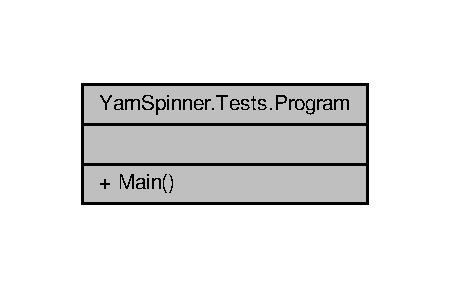
\includegraphics[width=224pt]{a00363}
\end{center}
\end{figure}
\subsection*{Public Types}
\begin{DoxyCompactItemize}
\item 
enum \hyperlink{a00038_ab24848d7951ce44eb3c7768c6ee10385}{State} \{ \hyperlink{a00038_ab24848d7951ce44eb3c7768c6ee10385a0197c47523ba5a2bdfef705786687de5}{State.\-Not\-Tested}, 
\hyperlink{a00038_ab24848d7951ce44eb3c7768c6ee10385ad96143ba1b15645919cea00ec9d1be62}{State.\-Ignored}, 
\hyperlink{a00038_ab24848d7951ce44eb3c7768c6ee10385aa0d0628f6b4e4d78d2ffef4d4d1c4b15}{State.\-Passed}, 
\hyperlink{a00038_ab24848d7951ce44eb3c7768c6ee10385ad7c8c85bf79bbe1b7188497c32c3b0ca}{State.\-Failed}
 \}
\end{DoxyCompactItemize}
\subsection*{Public Member Functions}
\begin{DoxyCompactItemize}
\item 
override bool \hyperlink{a00038_a1e653caad5ab99847c26ff8f67da8f45}{Equals} (object obj)
\item 
override int \hyperlink{a00038_a85d50993390cdd8ba30ac44043b18de7}{Get\-Hash\-Code} ()
\item 
\hyperlink{a00038_af1c9b3d1757d33ad2141c639c3827c97}{Checker\-Result} (Text\-Asset \hyperlink{a00038_a6c852f7521c0a91b519aa3d391f63e6b}{script})
\end{DoxyCompactItemize}
\subsection*{Public Attributes}
\begin{DoxyCompactItemize}
\item 
\hyperlink{a00038_ab24848d7951ce44eb3c7768c6ee10385}{State} \hyperlink{a00038_a7202b24bd068da24d7e28bec5668b13a}{state}
\item 
Text\-Asset \hyperlink{a00038_a6c852f7521c0a91b519aa3d391f63e6b}{script}
\item 
\hyperlink{a00099_a00185}{Validation\-Message}\mbox{[}$\,$\mbox{]} \hyperlink{a00038_a808a039e280cf875cb3c9e9385148498}{messages} = new \hyperlink{a00099_a00185}{Validation\-Message}\mbox{[}0\mbox{]}
\end{DoxyCompactItemize}


\subsection{Detailed Description}


\subsection{Member Enumeration Documentation}
\hypertarget{a00038_ab24848d7951ce44eb3c7768c6ee10385}{\index{Yarn\-::\-Unity\-::\-Yarn\-Spinner\-Editor\-Window\-::\-Checker\-Result@{Yarn\-::\-Unity\-::\-Yarn\-Spinner\-Editor\-Window\-::\-Checker\-Result}!State@{State}}
\index{State@{State}!Yarn::Unity::YarnSpinnerEditorWindow::CheckerResult@{Yarn\-::\-Unity\-::\-Yarn\-Spinner\-Editor\-Window\-::\-Checker\-Result}}
\subsubsection[{State}]{\setlength{\rightskip}{0pt plus 5cm}enum {\bf Yarn.\-Unity.\-Yarn\-Spinner\-Editor\-Window.\-Checker\-Result.\-State}}}\label{a00038_ab24848d7951ce44eb3c7768c6ee10385}
\begin{Desc}
\item[Enumerator]\par
\begin{description}
\index{Not\-Tested@{Not\-Tested}!Yarn\-::\-Unity\-::\-Yarn\-Spinner\-Editor\-Window\-::\-Checker\-Result@{Yarn\-::\-Unity\-::\-Yarn\-Spinner\-Editor\-Window\-::\-Checker\-Result}}\index{Yarn\-::\-Unity\-::\-Yarn\-Spinner\-Editor\-Window\-::\-Checker\-Result@{Yarn\-::\-Unity\-::\-Yarn\-Spinner\-Editor\-Window\-::\-Checker\-Result}!Not\-Tested@{Not\-Tested}}\item[{\em 
\hypertarget{a00038_ab24848d7951ce44eb3c7768c6ee10385a0197c47523ba5a2bdfef705786687de5}{Not\-Tested}\label{a00038_ab24848d7951ce44eb3c7768c6ee10385a0197c47523ba5a2bdfef705786687de5}
}]\index{Ignored@{Ignored}!Yarn\-::\-Unity\-::\-Yarn\-Spinner\-Editor\-Window\-::\-Checker\-Result@{Yarn\-::\-Unity\-::\-Yarn\-Spinner\-Editor\-Window\-::\-Checker\-Result}}\index{Yarn\-::\-Unity\-::\-Yarn\-Spinner\-Editor\-Window\-::\-Checker\-Result@{Yarn\-::\-Unity\-::\-Yarn\-Spinner\-Editor\-Window\-::\-Checker\-Result}!Ignored@{Ignored}}\item[{\em 
\hypertarget{a00038_ab24848d7951ce44eb3c7768c6ee10385ad96143ba1b15645919cea00ec9d1be62}{Ignored}\label{a00038_ab24848d7951ce44eb3c7768c6ee10385ad96143ba1b15645919cea00ec9d1be62}
}]\index{Passed@{Passed}!Yarn\-::\-Unity\-::\-Yarn\-Spinner\-Editor\-Window\-::\-Checker\-Result@{Yarn\-::\-Unity\-::\-Yarn\-Spinner\-Editor\-Window\-::\-Checker\-Result}}\index{Yarn\-::\-Unity\-::\-Yarn\-Spinner\-Editor\-Window\-::\-Checker\-Result@{Yarn\-::\-Unity\-::\-Yarn\-Spinner\-Editor\-Window\-::\-Checker\-Result}!Passed@{Passed}}\item[{\em 
\hypertarget{a00038_ab24848d7951ce44eb3c7768c6ee10385aa0d0628f6b4e4d78d2ffef4d4d1c4b15}{Passed}\label{a00038_ab24848d7951ce44eb3c7768c6ee10385aa0d0628f6b4e4d78d2ffef4d4d1c4b15}
}]\index{Failed@{Failed}!Yarn\-::\-Unity\-::\-Yarn\-Spinner\-Editor\-Window\-::\-Checker\-Result@{Yarn\-::\-Unity\-::\-Yarn\-Spinner\-Editor\-Window\-::\-Checker\-Result}}\index{Yarn\-::\-Unity\-::\-Yarn\-Spinner\-Editor\-Window\-::\-Checker\-Result@{Yarn\-::\-Unity\-::\-Yarn\-Spinner\-Editor\-Window\-::\-Checker\-Result}!Failed@{Failed}}\item[{\em 
\hypertarget{a00038_ab24848d7951ce44eb3c7768c6ee10385ad7c8c85bf79bbe1b7188497c32c3b0ca}{Failed}\label{a00038_ab24848d7951ce44eb3c7768c6ee10385ad7c8c85bf79bbe1b7188497c32c3b0ca}
}]\end{description}
\end{Desc}

\begin{DoxyCode}
36                               \{
37                 \hyperlink{a00038_ab24848d7951ce44eb3c7768c6ee10385a0197c47523ba5a2bdfef705786687de5}{NotTested},
38                 \hyperlink{a00038_ab24848d7951ce44eb3c7768c6ee10385ad96143ba1b15645919cea00ec9d1be62}{Ignored},
39                 \hyperlink{a00038_ab24848d7951ce44eb3c7768c6ee10385aa0d0628f6b4e4d78d2ffef4d4d1c4b15}{Passed},
40                 \hyperlink{a00038_ab24848d7951ce44eb3c7768c6ee10385ad7c8c85bf79bbe1b7188497c32c3b0ca}{Failed}
41             \}
\end{DoxyCode}


\subsection{Constructor \& Destructor Documentation}
\hypertarget{a00038_af1c9b3d1757d33ad2141c639c3827c97}{\index{Yarn\-::\-Unity\-::\-Yarn\-Spinner\-Editor\-Window\-::\-Checker\-Result@{Yarn\-::\-Unity\-::\-Yarn\-Spinner\-Editor\-Window\-::\-Checker\-Result}!Checker\-Result@{Checker\-Result}}
\index{Checker\-Result@{Checker\-Result}!Yarn::Unity::YarnSpinnerEditorWindow::CheckerResult@{Yarn\-::\-Unity\-::\-Yarn\-Spinner\-Editor\-Window\-::\-Checker\-Result}}
\subsubsection[{Checker\-Result}]{\setlength{\rightskip}{0pt plus 5cm}Yarn.\-Unity.\-Yarn\-Spinner\-Editor\-Window.\-Checker\-Result.\-Checker\-Result (
\begin{DoxyParamCaption}
\item[{Text\-Asset}]{script}
\end{DoxyParamCaption}
)}}\label{a00038_af1c9b3d1757d33ad2141c639c3827c97}

\begin{DoxyCode}
61                                                    \{
62                 this.script = \hyperlink{a00038_a6c852f7521c0a91b519aa3d391f63e6b}{script};
63                 this.state = State.NotTested;
64             \}
\end{DoxyCode}


\subsection{Member Function Documentation}
\hypertarget{a00038_a1e653caad5ab99847c26ff8f67da8f45}{\index{Yarn\-::\-Unity\-::\-Yarn\-Spinner\-Editor\-Window\-::\-Checker\-Result@{Yarn\-::\-Unity\-::\-Yarn\-Spinner\-Editor\-Window\-::\-Checker\-Result}!Equals@{Equals}}
\index{Equals@{Equals}!Yarn::Unity::YarnSpinnerEditorWindow::CheckerResult@{Yarn\-::\-Unity\-::\-Yarn\-Spinner\-Editor\-Window\-::\-Checker\-Result}}
\subsubsection[{Equals}]{\setlength{\rightskip}{0pt plus 5cm}override bool Yarn.\-Unity.\-Yarn\-Spinner\-Editor\-Window.\-Checker\-Result.\-Equals (
\begin{DoxyParamCaption}
\item[{object}]{obj}
\end{DoxyParamCaption}
)}}\label{a00038_a1e653caad5ab99847c26ff8f67da8f45}

\begin{DoxyCode}
49             \{
50                 \textcolor{keywordflow}{if} (obj is \hyperlink{a00038_af1c9b3d1757d33ad2141c639c3827c97}{CheckerResult} && ((\hyperlink{a00038_af1c9b3d1757d33ad2141c639c3827c97}{CheckerResult})obj).
      \hyperlink{a00038_a6c852f7521c0a91b519aa3d391f63e6b}{script} == this.\hyperlink{a00038_a6c852f7521c0a91b519aa3d391f63e6b}{script})
51                     \textcolor{keywordflow}{return} \textcolor{keyword}{true};
52                 \textcolor{keywordflow}{else}
53                     \textcolor{keywordflow}{return} \textcolor{keyword}{false};
54             \}
\end{DoxyCode}
\hypertarget{a00038_a85d50993390cdd8ba30ac44043b18de7}{\index{Yarn\-::\-Unity\-::\-Yarn\-Spinner\-Editor\-Window\-::\-Checker\-Result@{Yarn\-::\-Unity\-::\-Yarn\-Spinner\-Editor\-Window\-::\-Checker\-Result}!Get\-Hash\-Code@{Get\-Hash\-Code}}
\index{Get\-Hash\-Code@{Get\-Hash\-Code}!Yarn::Unity::YarnSpinnerEditorWindow::CheckerResult@{Yarn\-::\-Unity\-::\-Yarn\-Spinner\-Editor\-Window\-::\-Checker\-Result}}
\subsubsection[{Get\-Hash\-Code}]{\setlength{\rightskip}{0pt plus 5cm}override int Yarn.\-Unity.\-Yarn\-Spinner\-Editor\-Window.\-Checker\-Result.\-Get\-Hash\-Code (
\begin{DoxyParamCaption}
{}
\end{DoxyParamCaption}
)}}\label{a00038_a85d50993390cdd8ba30ac44043b18de7}

\begin{DoxyCode}
57             \{
58                 \textcolor{keywordflow}{return} this.script.GetHashCode();
59             \}
\end{DoxyCode}


\subsection{Member Data Documentation}
\hypertarget{a00038_a808a039e280cf875cb3c9e9385148498}{\index{Yarn\-::\-Unity\-::\-Yarn\-Spinner\-Editor\-Window\-::\-Checker\-Result@{Yarn\-::\-Unity\-::\-Yarn\-Spinner\-Editor\-Window\-::\-Checker\-Result}!messages@{messages}}
\index{messages@{messages}!Yarn::Unity::YarnSpinnerEditorWindow::CheckerResult@{Yarn\-::\-Unity\-::\-Yarn\-Spinner\-Editor\-Window\-::\-Checker\-Result}}
\subsubsection[{messages}]{\setlength{\rightskip}{0pt plus 5cm}{\bf Validation\-Message} \mbox{[}$\,$\mbox{]} Yarn.\-Unity.\-Yarn\-Spinner\-Editor\-Window.\-Checker\-Result.\-messages = new {\bf Validation\-Message}\mbox{[}0\mbox{]}}}\label{a00038_a808a039e280cf875cb3c9e9385148498}
\hypertarget{a00038_a6c852f7521c0a91b519aa3d391f63e6b}{\index{Yarn\-::\-Unity\-::\-Yarn\-Spinner\-Editor\-Window\-::\-Checker\-Result@{Yarn\-::\-Unity\-::\-Yarn\-Spinner\-Editor\-Window\-::\-Checker\-Result}!script@{script}}
\index{script@{script}!Yarn::Unity::YarnSpinnerEditorWindow::CheckerResult@{Yarn\-::\-Unity\-::\-Yarn\-Spinner\-Editor\-Window\-::\-Checker\-Result}}
\subsubsection[{script}]{\setlength{\rightskip}{0pt plus 5cm}Text\-Asset Yarn.\-Unity.\-Yarn\-Spinner\-Editor\-Window.\-Checker\-Result.\-script}}\label{a00038_a6c852f7521c0a91b519aa3d391f63e6b}
\hypertarget{a00038_a7202b24bd068da24d7e28bec5668b13a}{\index{Yarn\-::\-Unity\-::\-Yarn\-Spinner\-Editor\-Window\-::\-Checker\-Result@{Yarn\-::\-Unity\-::\-Yarn\-Spinner\-Editor\-Window\-::\-Checker\-Result}!state@{state}}
\index{state@{state}!Yarn::Unity::YarnSpinnerEditorWindow::CheckerResult@{Yarn\-::\-Unity\-::\-Yarn\-Spinner\-Editor\-Window\-::\-Checker\-Result}}
\subsubsection[{state}]{\setlength{\rightskip}{0pt plus 5cm}{\bf State} Yarn.\-Unity.\-Yarn\-Spinner\-Editor\-Window.\-Checker\-Result.\-state}}\label{a00038_a7202b24bd068da24d7e28bec5668b13a}


The documentation for this class was generated from the following file\-:\begin{DoxyCompactItemize}
\item 
Unity/\-Assets/\-Yarn Spinner/\-Code/\-Editor/\hyperlink{a00127}{Yarn\-Spinner\-Editor\-Window.\-cs}\end{DoxyCompactItemize}

\hypertarget{a00039}{\section{Csv\-Helper.\-Type\-Conversion.\-Boolean\-Converter Class Reference}
\label{a00039}\index{Csv\-Helper.\-Type\-Conversion.\-Boolean\-Converter@{Csv\-Helper.\-Type\-Conversion.\-Boolean\-Converter}}
}


Converts a Boolean to and from a string.  




Inheritance diagram for Csv\-Helper.\-Type\-Conversion.\-Boolean\-Converter\-:
\nopagebreak
\begin{figure}[H]
\begin{center}
\leavevmode
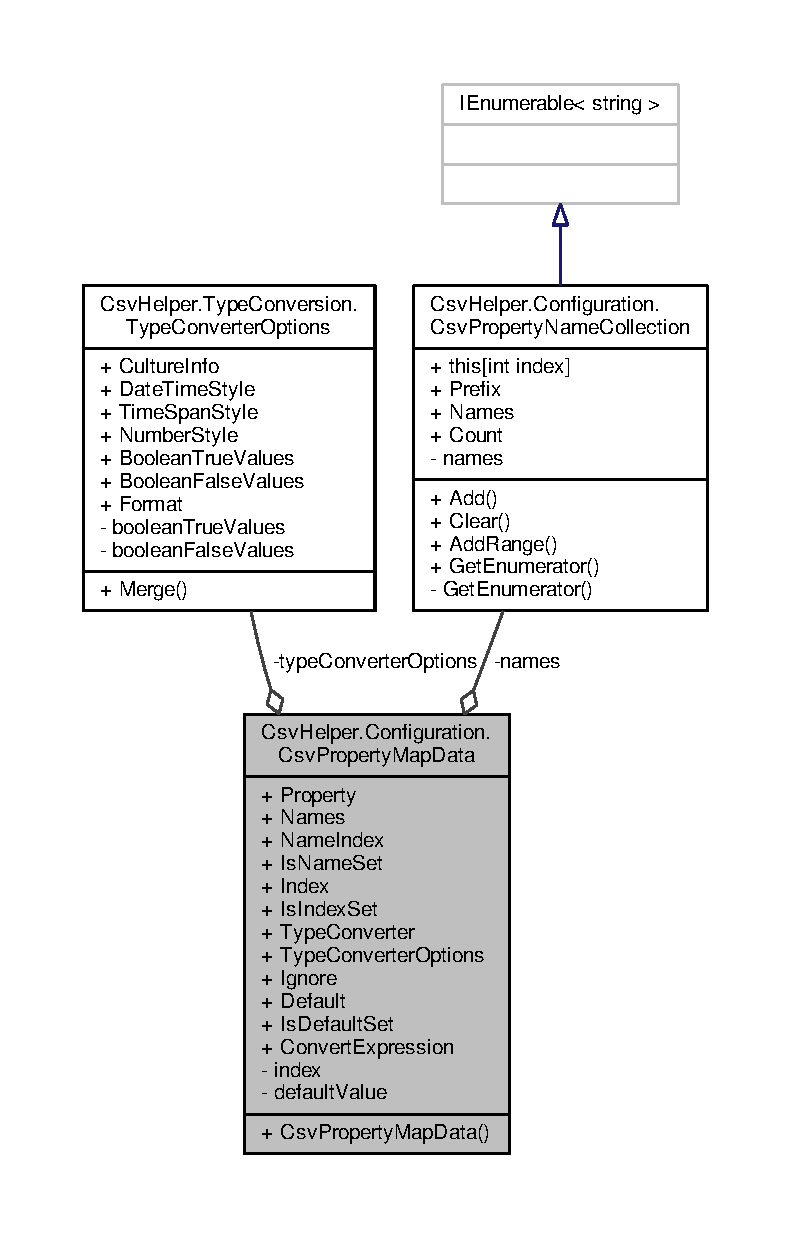
\includegraphics[width=220pt]{a00497}
\end{center}
\end{figure}


Collaboration diagram for Csv\-Helper.\-Type\-Conversion.\-Boolean\-Converter\-:
\nopagebreak
\begin{figure}[H]
\begin{center}
\leavevmode
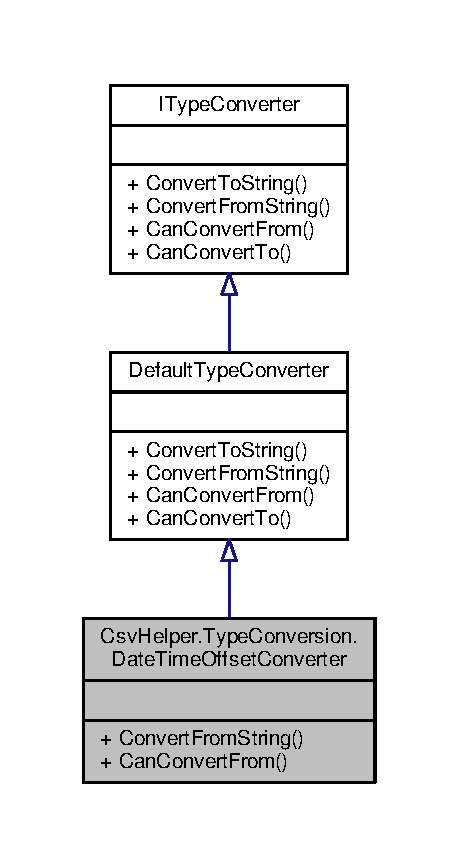
\includegraphics[width=220pt]{a00498}
\end{center}
\end{figure}
\subsection*{Public Member Functions}
\begin{DoxyCompactItemize}
\item 
override object \hyperlink{a00039_abc77c631974272fd1dfe3fe4fcc3bf28}{Convert\-From\-String} (\hyperlink{a00172}{Type\-Converter\-Options} options, string text)
\begin{DoxyCompactList}\small\item\em Converts the string to an object. \end{DoxyCompactList}\item 
override bool \hyperlink{a00039_a0be20573af4ee53409bb437125a64268}{Can\-Convert\-From} (Type type)
\begin{DoxyCompactList}\small\item\em Determines whether this instance \mbox{[}can convert from\mbox{]} the specified type. \end{DoxyCompactList}\item 
virtual string \hyperlink{a00082_a36cb2f9b24f15a671293f3a722324c27}{Convert\-To\-String} (\hyperlink{a00172}{Type\-Converter\-Options} options, object value)
\begin{DoxyCompactList}\small\item\em Converts the object to a string. \end{DoxyCompactList}\item 
virtual bool \hyperlink{a00082_acb65bd8c8199d88d5b1629ae35d18514}{Can\-Convert\-To} (Type type)
\begin{DoxyCompactList}\small\item\em Determines whether this instance \mbox{[}can convert to\mbox{]} the specified type. \end{DoxyCompactList}\end{DoxyCompactItemize}


\subsection{Detailed Description}
Converts a Boolean to and from a string. 



Definition at line 13 of file Boolean\-Converter.\-cs.



\subsection{Member Function Documentation}
\hypertarget{a00039_a0be20573af4ee53409bb437125a64268}{\index{Csv\-Helper\-::\-Type\-Conversion\-::\-Boolean\-Converter@{Csv\-Helper\-::\-Type\-Conversion\-::\-Boolean\-Converter}!Can\-Convert\-From@{Can\-Convert\-From}}
\index{Can\-Convert\-From@{Can\-Convert\-From}!CsvHelper::TypeConversion::BooleanConverter@{Csv\-Helper\-::\-Type\-Conversion\-::\-Boolean\-Converter}}
\subsubsection[{Can\-Convert\-From}]{\setlength{\rightskip}{0pt plus 5cm}override bool Csv\-Helper.\-Type\-Conversion.\-Boolean\-Converter.\-Can\-Convert\-From (
\begin{DoxyParamCaption}
\item[{Type}]{type}
\end{DoxyParamCaption}
)\hspace{0.3cm}{\ttfamily [virtual]}}}\label{a00039_a0be20573af4ee53409bb437125a64268}


Determines whether this instance \mbox{[}can convert from\mbox{]} the specified type. 


\begin{DoxyParams}{Parameters}
{\em type} & The type.\\
\hline
\end{DoxyParams}
\begin{DoxyReturn}{Returns}
{\ttfamily true} if this instance \mbox{[}can convert from\mbox{]} the specified type; otherwise, {\ttfamily false}. 
\end{DoxyReturn}


Reimplemented from \hyperlink{a00082_a470d21adaa704eb281250dbd112ff91a}{Csv\-Helper.\-Type\-Conversion.\-Default\-Type\-Converter}.



Definition at line 69 of file Boolean\-Converter.\-cs.


\begin{DoxyCode}
70         \{
71             \textcolor{comment}{// We only care about strings.}
72             \textcolor{keywordflow}{return} type == typeof( \textcolor{keywordtype}{string} );
73         \}
\end{DoxyCode}
\hypertarget{a00082_acb65bd8c8199d88d5b1629ae35d18514}{\index{Csv\-Helper\-::\-Type\-Conversion\-::\-Boolean\-Converter@{Csv\-Helper\-::\-Type\-Conversion\-::\-Boolean\-Converter}!Can\-Convert\-To@{Can\-Convert\-To}}
\index{Can\-Convert\-To@{Can\-Convert\-To}!CsvHelper::TypeConversion::BooleanConverter@{Csv\-Helper\-::\-Type\-Conversion\-::\-Boolean\-Converter}}
\subsubsection[{Can\-Convert\-To}]{\setlength{\rightskip}{0pt plus 5cm}virtual bool Csv\-Helper.\-Type\-Conversion.\-Default\-Type\-Converter.\-Can\-Convert\-To (
\begin{DoxyParamCaption}
\item[{Type}]{type}
\end{DoxyParamCaption}
)\hspace{0.3cm}{\ttfamily [virtual]}, {\ttfamily [inherited]}}}\label{a00082_acb65bd8c8199d88d5b1629ae35d18514}


Determines whether this instance \mbox{[}can convert to\mbox{]} the specified type. 


\begin{DoxyParams}{Parameters}
{\em type} & The type.\\
\hline
\end{DoxyParams}
\begin{DoxyReturn}{Returns}
{\ttfamily true} if this instance \mbox{[}can convert to\mbox{]} the specified type; otherwise, {\ttfamily false}. 
\end{DoxyReturn}


Implements \hyperlink{a00117_a168b03dad37fcb6882101c93deac8111}{Csv\-Helper.\-Type\-Conversion.\-I\-Type\-Converter}.



Reimplemented in \hyperlink{a00093_a44d625b44f770b945a29cd89e399f90f}{Csv\-Helper.\-Type\-Conversion.\-Enumerable\-Converter}.



Definition at line 69 of file Default\-Type\-Converter.\-cs.


\begin{DoxyCode}
70         \{
71             \textcolor{comment}{// We only care about strings.}
72             \textcolor{keywordflow}{return} type == typeof( \textcolor{keywordtype}{string} );
73         \}
\end{DoxyCode}
\hypertarget{a00039_abc77c631974272fd1dfe3fe4fcc3bf28}{\index{Csv\-Helper\-::\-Type\-Conversion\-::\-Boolean\-Converter@{Csv\-Helper\-::\-Type\-Conversion\-::\-Boolean\-Converter}!Convert\-From\-String@{Convert\-From\-String}}
\index{Convert\-From\-String@{Convert\-From\-String}!CsvHelper::TypeConversion::BooleanConverter@{Csv\-Helper\-::\-Type\-Conversion\-::\-Boolean\-Converter}}
\subsubsection[{Convert\-From\-String}]{\setlength{\rightskip}{0pt plus 5cm}override object Csv\-Helper.\-Type\-Conversion.\-Boolean\-Converter.\-Convert\-From\-String (
\begin{DoxyParamCaption}
\item[{{\bf Type\-Converter\-Options}}]{options, }
\item[{string}]{text}
\end{DoxyParamCaption}
)\hspace{0.3cm}{\ttfamily [virtual]}}}\label{a00039_abc77c631974272fd1dfe3fe4fcc3bf28}


Converts the string to an object. 


\begin{DoxyParams}{Parameters}
{\em options} & The options to use when converting.\\
\hline
{\em text} & The string to convert to an object.\\
\hline
\end{DoxyParams}
\begin{DoxyReturn}{Returns}
The object created from the string.
\end{DoxyReturn}


Reimplemented from \hyperlink{a00082_a804ea00060e1de70e5151f90d3bfce9b}{Csv\-Helper.\-Type\-Conversion.\-Default\-Type\-Converter}.



Definition at line 21 of file Boolean\-Converter.\-cs.


\begin{DoxyCode}
22         \{
23             \textcolor{keywordtype}{bool} b;
24             \textcolor{keywordflow}{if}( \textcolor{keywordtype}{bool}.TryParse( text, out b ) )
25             \{
26                 \textcolor{keywordflow}{return} b;
27             \}
28 
29             \textcolor{keywordtype}{short} sh;
30             \textcolor{keywordflow}{if}( \textcolor{keywordtype}{short}.TryParse( text, out sh ) )
31             \{
32                 \textcolor{keywordflow}{if}( sh == 0 )
33                 \{
34                     \textcolor{keywordflow}{return} \textcolor{keyword}{false};
35                 \}
36                 \textcolor{keywordflow}{if}( sh == 1 )
37                 \{
38                     \textcolor{keywordflow}{return} \textcolor{keyword}{true};
39                 \}
40             \}
41 
42             var t = ( text ?? string.Empty ).Trim();
43             \textcolor{keywordflow}{foreach}( var trueValue \textcolor{keywordflow}{in} options.BooleanTrueValues )
44             \{
45                 \textcolor{keywordflow}{if}( options.CultureInfo.CompareInfo.Compare( trueValue, t, CompareOptions.IgnoreCase ) == 0
       )
46                 \{
47                     \textcolor{keywordflow}{return} \textcolor{keyword}{true};
48                 \}
49             \}
50 
51             \textcolor{keywordflow}{foreach}( var falseValue \textcolor{keywordflow}{in} options.BooleanFalseValues )
52             \{
53                 \textcolor{keywordflow}{if}( options.CultureInfo.CompareInfo.Compare( falseValue, t, CompareOptions.IgnoreCase ) == 
      0 )
54                 \{
55                     \textcolor{keywordflow}{return} \textcolor{keyword}{false};
56                 \}
57             \}
58 
59             \textcolor{keywordflow}{return} base.ConvertFromString( options, text );
60         \}
\end{DoxyCode}
\hypertarget{a00082_a36cb2f9b24f15a671293f3a722324c27}{\index{Csv\-Helper\-::\-Type\-Conversion\-::\-Boolean\-Converter@{Csv\-Helper\-::\-Type\-Conversion\-::\-Boolean\-Converter}!Convert\-To\-String@{Convert\-To\-String}}
\index{Convert\-To\-String@{Convert\-To\-String}!CsvHelper::TypeConversion::BooleanConverter@{Csv\-Helper\-::\-Type\-Conversion\-::\-Boolean\-Converter}}
\subsubsection[{Convert\-To\-String}]{\setlength{\rightskip}{0pt plus 5cm}virtual string Csv\-Helper.\-Type\-Conversion.\-Default\-Type\-Converter.\-Convert\-To\-String (
\begin{DoxyParamCaption}
\item[{{\bf Type\-Converter\-Options}}]{options, }
\item[{object}]{value}
\end{DoxyParamCaption}
)\hspace{0.3cm}{\ttfamily [virtual]}, {\ttfamily [inherited]}}}\label{a00082_a36cb2f9b24f15a671293f3a722324c27}


Converts the object to a string. 


\begin{DoxyParams}{Parameters}
{\em options} & The options to use when converting.\\
\hline
{\em value} & The object to convert to a string.\\
\hline
\end{DoxyParams}
\begin{DoxyReturn}{Returns}
The string representation of the object.
\end{DoxyReturn}


Implements \hyperlink{a00117_a90c465c63dbcf913f38aa878f35e77c7}{Csv\-Helper.\-Type\-Conversion.\-I\-Type\-Converter}.



Reimplemented in \hyperlink{a00136_a7205cdb61d2d119582958232b3e63109}{Csv\-Helper.\-Type\-Conversion.\-Nullable\-Converter}, and \hyperlink{a00093_a7e07e9532857d748654d37db590a0e11}{Csv\-Helper.\-Type\-Conversion.\-Enumerable\-Converter}.



Definition at line 21 of file Default\-Type\-Converter.\-cs.


\begin{DoxyCode}
22         \{
23             \textcolor{keywordflow}{if}( value == null )
24             \{
25                 \textcolor{keywordflow}{return} string.Empty;
26             \}
27 
28             var formattable = value as IFormattable;
29             \textcolor{keywordflow}{if}( formattable != null )
30             \{
31                 \textcolor{keywordflow}{return} formattable.ToString( options.Format, options.CultureInfo );
32             \}
33 
34             \textcolor{keywordflow}{return} value.ToString();
35         \}
\end{DoxyCode}


The documentation for this class was generated from the following file\-:\begin{DoxyCompactItemize}
\item 
packages/\-Csv\-Helper.\-2.\-16.\-0.\-0/src/\-Csv\-Helper/\-Type\-Conversion/\hyperlink{a00256}{Boolean\-Converter.\-cs}\end{DoxyCompactItemize}

\hypertarget{a00033}{\section{Example\-Variable\-Storage Class Reference}
\label{a00033}\index{Example\-Variable\-Storage@{Example\-Variable\-Storage}}
}


Inheritance diagram for Example\-Variable\-Storage\-:
\nopagebreak
\begin{figure}[H]
\begin{center}
\leavevmode
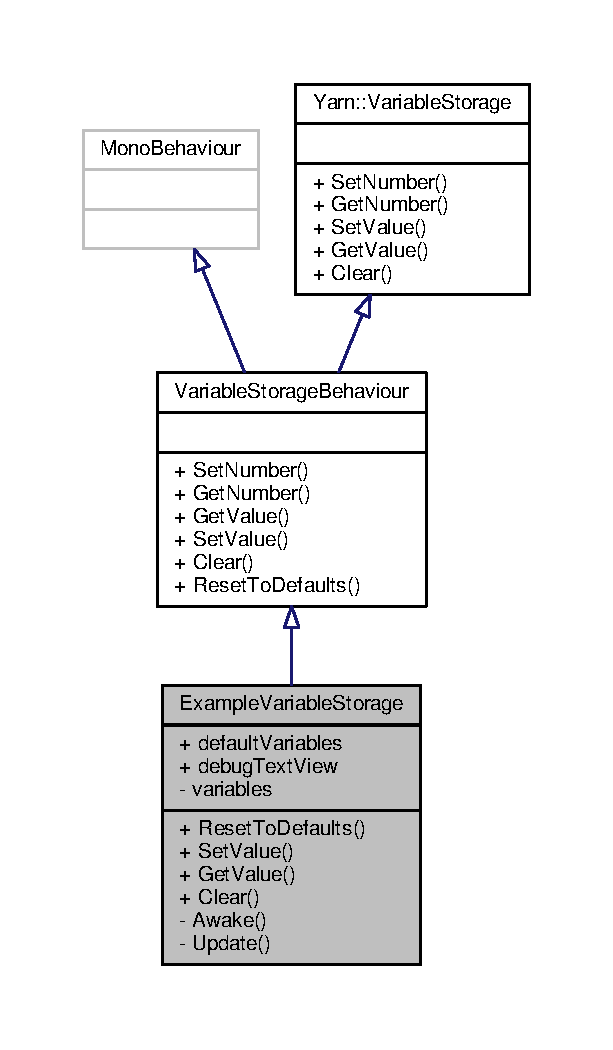
\includegraphics[width=294pt]{dd/d4c/a00177}
\end{center}
\end{figure}


Collaboration diagram for Example\-Variable\-Storage\-:
\nopagebreak
\begin{figure}[H]
\begin{center}
\leavevmode
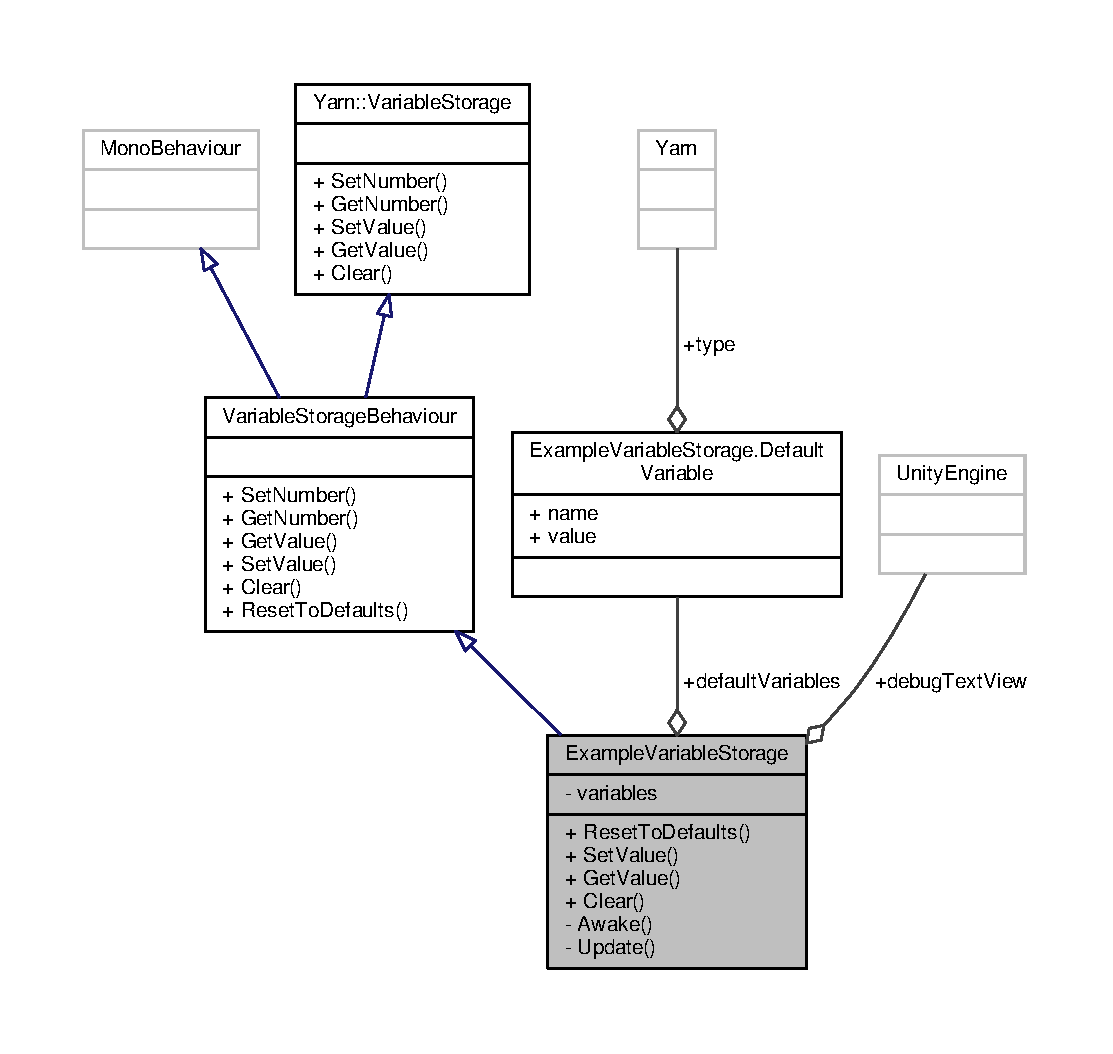
\includegraphics[width=350pt]{d9/d90/a00178}
\end{center}
\end{figure}
\subsection*{Classes}
\begin{DoxyCompactItemize}
\item 
class \hyperlink{a00033_de/d38/a00160}{Default\-Variable}
\end{DoxyCompactItemize}
\subsection*{Public Member Functions}
\begin{DoxyCompactItemize}
\item 
override void \hyperlink{a00033_a3a05d66cdacadb2e9b618cd0aef45f84}{Reset\-To\-Defaults} ()
\item 
override void \hyperlink{a00033_ac4265c1c9da485f13a6b05784b0f668d}{Set\-Value} (string variable\-Name, \hyperlink{a00086}{Yarn.\-Value} value)
\item 
override \hyperlink{a00086}{Yarn.\-Value} \hyperlink{a00033_a741593be1a299dcc2136f05b9b4a995a}{Get\-Value} (string variable\-Name)
\item 
override void \hyperlink{a00033_a0ce614bee8d5b220500fb765390b4ca3}{Clear} ()
\item 
virtual void \hyperlink{a00089_ac0d2f2e081944ad197992a26ad1a833c}{Set\-Number} (string variable\-Name, float number)
\item 
virtual float \hyperlink{a00089_add85a45dd65a5d4bd41c9d5ce5f77d19}{Get\-Number} (string variable\-Name)
\end{DoxyCompactItemize}
\subsection*{Public Attributes}
\begin{DoxyCompactItemize}
\item 
\hyperlink{a00033_de/d38/a00160}{Default\-Variable}\mbox{[}$\,$\mbox{]} \hyperlink{a00033_a464c8a4ff6a3c624602d0adc55dfc59a}{default\-Variables}
\item 
Unity\-Engine.\-U\-I.\-Text \hyperlink{a00033_a9893656e3683711eb78441b30c52a600}{debug\-Text\-View}
\end{DoxyCompactItemize}
\subsection*{Private Member Functions}
\begin{DoxyCompactItemize}
\item 
void \hyperlink{a00033_ab6a56afc687455f360876eff67891163}{Awake} ()
\item 
void \hyperlink{a00033_af646a17cfd63039a25149f8fc0776dcb}{Update} ()
\end{DoxyCompactItemize}
\subsection*{Private Attributes}
\begin{DoxyCompactItemize}
\item 
Dictionary$<$ string, \hyperlink{a00086}{Yarn.\-Value} $>$ \hyperlink{a00033_a4a4fec7b4ad707cd0603393dd57de96c}{variables} = new Dictionary$<$string, \hyperlink{a00086}{Yarn.\-Value}$>$ ()
\end{DoxyCompactItemize}


\subsection{Detailed Description}


\subsection{Class Documentation}
\index{Example\-Variable\-Storage\-::\-Default\-Variable@{Example\-Variable\-Storage\-::\-Default\-Variable}}\label{de/d38/a00160}
\hypertarget{a00033_de/d38/a00160}{}
\subsubsection{class Example\-Variable\-Storage\-:\-:Default\-Variable}


Collaboration diagram for Example\-Variable\-Storage.\-Default\-Variable\-:
\nopagebreak
\begin{figure}[H]
\begin{center}
\leavevmode
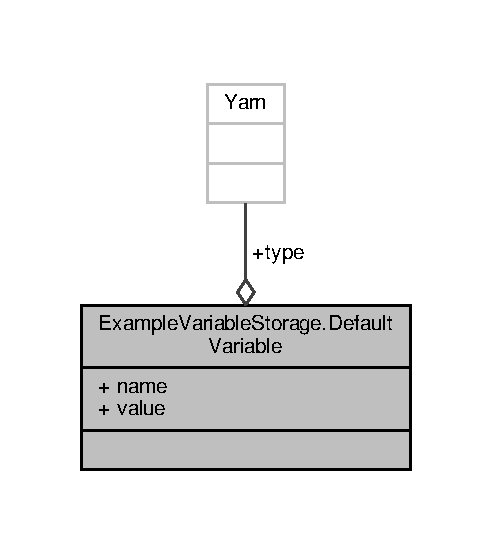
\includegraphics[width=236pt]{dd/da7/a00168}
\end{center}
\end{figure}
\begin{DoxyFields}{Class Members}
\hypertarget{a00033_a609feaa53936e7dc42248ff2ba68454a}{string}\label{a00033_a609feaa53936e7dc42248ff2ba68454a}
&
name&
\\
\hline

\hypertarget{a00033_a904347efdca12f40243c7dedb646153d}{Value}\label{a00033_a904347efdca12f40243c7dedb646153d}
&
type&
\\
\hline

\hypertarget{a00033_a0f00ecb21b58aa754a4bbb61edf62818}{string}\label{a00033_a0f00ecb21b58aa754a4bbb61edf62818}
&
value&
\\
\hline

\end{DoxyFields}


\subsection{Member Function Documentation}
\hypertarget{a00033_ab6a56afc687455f360876eff67891163}{\index{Example\-Variable\-Storage@{Example\-Variable\-Storage}!Awake@{Awake}}
\index{Awake@{Awake}!ExampleVariableStorage@{Example\-Variable\-Storage}}
\subsubsection[{Awake}]{\setlength{\rightskip}{0pt plus 5cm}void Example\-Variable\-Storage.\-Awake (
\begin{DoxyParamCaption}
{}
\end{DoxyParamCaption}
)\hspace{0.3cm}{\ttfamily [private]}}}\label{a00033_ab6a56afc687455f360876eff67891163}

\begin{DoxyCode}
59     \{
60         \hyperlink{a00033_a3a05d66cdacadb2e9b618cd0aef45f84}{ResetToDefaults} ();
61     \}
\end{DoxyCode}
\hypertarget{a00033_a0ce614bee8d5b220500fb765390b4ca3}{\index{Example\-Variable\-Storage@{Example\-Variable\-Storage}!Clear@{Clear}}
\index{Clear@{Clear}!ExampleVariableStorage@{Example\-Variable\-Storage}}
\subsubsection[{Clear}]{\setlength{\rightskip}{0pt plus 5cm}override void Example\-Variable\-Storage.\-Clear (
\begin{DoxyParamCaption}
{}
\end{DoxyParamCaption}
)\hspace{0.3cm}{\ttfamily [virtual]}}}\label{a00033_a0ce614bee8d5b220500fb765390b4ca3}


Reimplemented from \hyperlink{a00089_a587fe10b367ace190e10f3bcb590a53c}{Yarn.\-Unity.\-Variable\-Storage\-Behaviour}.


\begin{DoxyCode}
141     \{
142         variables.Clear ();
143     \}
\end{DoxyCode}
\hypertarget{a00089_add85a45dd65a5d4bd41c9d5ce5f77d19}{\index{Example\-Variable\-Storage@{Example\-Variable\-Storage}!Get\-Number@{Get\-Number}}
\index{Get\-Number@{Get\-Number}!ExampleVariableStorage@{Example\-Variable\-Storage}}
\subsubsection[{Get\-Number}]{\setlength{\rightskip}{0pt plus 5cm}virtual float Yarn.\-Unity.\-Variable\-Storage\-Behaviour.\-Get\-Number (
\begin{DoxyParamCaption}
\item[{string}]{variable\-Name}
\end{DoxyParamCaption}
)\hspace{0.3cm}{\ttfamily [virtual]}, {\ttfamily [inherited]}}}\label{a00089_add85a45dd65a5d4bd41c9d5ce5f77d19}


Implements \hyperlink{a00088_a04b061c52d8ac814ce559da5286fbc71}{Yarn.\-Variable\-Storage}.


\begin{DoxyCode}
375         \{
376             \textcolor{keywordflow}{throw} \textcolor{keyword}{new} System.NotImplementedException ();
377         \}
\end{DoxyCode}
\hypertarget{a00033_a741593be1a299dcc2136f05b9b4a995a}{\index{Example\-Variable\-Storage@{Example\-Variable\-Storage}!Get\-Value@{Get\-Value}}
\index{Get\-Value@{Get\-Value}!ExampleVariableStorage@{Example\-Variable\-Storage}}
\subsubsection[{Get\-Value}]{\setlength{\rightskip}{0pt plus 5cm}override {\bf Yarn.\-Value} Example\-Variable\-Storage.\-Get\-Value (
\begin{DoxyParamCaption}
\item[{string}]{variable\-Name}
\end{DoxyParamCaption}
)\hspace{0.3cm}{\ttfamily [virtual]}}}\label{a00033_a741593be1a299dcc2136f05b9b4a995a}


Reimplemented from \hyperlink{a00089_ac6ebafcbebc2b2d71eba8562490a2f1e}{Yarn.\-Unity.\-Variable\-Storage\-Behaviour}.


\begin{DoxyCode}
131     \{
132         \textcolor{comment}{// If we don't have a variable with this name, return the null value}
133         \textcolor{keywordflow}{if} (\hyperlink{a00033_a4a4fec7b4ad707cd0603393dd57de96c}{variables}.ContainsKey(variableName) == \textcolor{keyword}{false})
134             \textcolor{keywordflow}{return} Yarn.Value.NULL;
135         
136         \textcolor{keywordflow}{return} \hyperlink{a00033_a4a4fec7b4ad707cd0603393dd57de96c}{variables} [variableName];
137     \}
\end{DoxyCode}
\hypertarget{a00033_a3a05d66cdacadb2e9b618cd0aef45f84}{\index{Example\-Variable\-Storage@{Example\-Variable\-Storage}!Reset\-To\-Defaults@{Reset\-To\-Defaults}}
\index{Reset\-To\-Defaults@{Reset\-To\-Defaults}!ExampleVariableStorage@{Example\-Variable\-Storage}}
\subsubsection[{Reset\-To\-Defaults}]{\setlength{\rightskip}{0pt plus 5cm}override void Example\-Variable\-Storage.\-Reset\-To\-Defaults (
\begin{DoxyParamCaption}
{}
\end{DoxyParamCaption}
)\hspace{0.3cm}{\ttfamily [virtual]}}}\label{a00033_a3a05d66cdacadb2e9b618cd0aef45f84}


Implements \hyperlink{a00089_a33fcbff56561e53e0a70b59c56f0c3af}{Yarn.\-Unity.\-Variable\-Storage\-Behaviour}.


\begin{DoxyCode}
65     \{
66         \hyperlink{a00033_a0ce614bee8d5b220500fb765390b4ca3}{Clear} ();
67         
68         \textcolor{comment}{// For each default variable that's been defined, parse the string}
69         \textcolor{comment}{// that the user typed in in Unity and store the variable}
70         \textcolor{keywordflow}{foreach} (var variable \textcolor{keywordflow}{in} \hyperlink{a00033_a464c8a4ff6a3c624602d0adc55dfc59a}{defaultVariables}) \{
71             
72             \textcolor{keywordtype}{object} value;
73 
74             \textcolor{keywordflow}{switch} (variable.type) \{
75             \textcolor{keywordflow}{case} Yarn.Value.Type.Number:
76                 \textcolor{keywordtype}{float} f = 0.0f;
77 
78                 float.TryParse(variable.value, out f);
79 
80                 value = f;
81 
82                 \textcolor{keywordflow}{break};
83 
84             \textcolor{keywordflow}{case} Yarn.Value.Type.String:
85 
86                 value = variable.value;
87 
88                 \textcolor{keywordflow}{break};
89             \textcolor{keywordflow}{case} Yarn.Value.Type.Bool:
90 
91                 \textcolor{keywordtype}{bool} b = \textcolor{keyword}{false};
92 
93                 bool.TryParse(variable.value, out b);
94 
95                 value = b;
96 
97                 \textcolor{keywordflow}{break};
98             \textcolor{keywordflow}{case} Yarn.Value.Type.Variable:
99 
100                 \textcolor{comment}{// We don't support assigning default variables from other variables}
101                 \textcolor{comment}{// yet}
102                 Debug.LogErrorFormat(\textcolor{stringliteral}{"Can't set variable \{0\} to \{1\}: You can't "} +
103                     \textcolor{stringliteral}{"set a default variable to be another variable, because it "} +
104                     \textcolor{stringliteral}{"may not have been initialised yet."}, variable.name, variable.value);
105                 \textcolor{keywordflow}{continue};
106 
107             \textcolor{keywordflow}{case} Yarn.Value.Type.Null:
108 
109                 value = null;
110 
111                 \textcolor{keywordflow}{break};
112             \textcolor{keywordflow}{default}:
113                 \textcolor{keywordflow}{throw} \textcolor{keyword}{new} System.ArgumentOutOfRangeException ();
114             \}
115 
116             var v = \textcolor{keyword}{new} \hyperlink{a00086}{Yarn.Value}(value);
117 
118             \hyperlink{a00033_ac4265c1c9da485f13a6b05784b0f668d}{SetValue} (\textcolor{stringliteral}{"$"} + variable.name, v);
119         \}
120     \}
\end{DoxyCode}
\hypertarget{a00089_ac0d2f2e081944ad197992a26ad1a833c}{\index{Example\-Variable\-Storage@{Example\-Variable\-Storage}!Set\-Number@{Set\-Number}}
\index{Set\-Number@{Set\-Number}!ExampleVariableStorage@{Example\-Variable\-Storage}}
\subsubsection[{Set\-Number}]{\setlength{\rightskip}{0pt plus 5cm}virtual void Yarn.\-Unity.\-Variable\-Storage\-Behaviour.\-Set\-Number (
\begin{DoxyParamCaption}
\item[{string}]{variable\-Name, }
\item[{float}]{number}
\end{DoxyParamCaption}
)\hspace{0.3cm}{\ttfamily [virtual]}, {\ttfamily [inherited]}}}\label{a00089_ac0d2f2e081944ad197992a26ad1a833c}


Implements \hyperlink{a00088_aa28c3694f985cf73489efc301b9d41dd}{Yarn.\-Variable\-Storage}.


\begin{DoxyCode}
370         \{
371             \textcolor{keywordflow}{throw} \textcolor{keyword}{new} System.NotImplementedException ();
372         \}
\end{DoxyCode}
\hypertarget{a00033_ac4265c1c9da485f13a6b05784b0f668d}{\index{Example\-Variable\-Storage@{Example\-Variable\-Storage}!Set\-Value@{Set\-Value}}
\index{Set\-Value@{Set\-Value}!ExampleVariableStorage@{Example\-Variable\-Storage}}
\subsubsection[{Set\-Value}]{\setlength{\rightskip}{0pt plus 5cm}override void Example\-Variable\-Storage.\-Set\-Value (
\begin{DoxyParamCaption}
\item[{string}]{variable\-Name, }
\item[{{\bf Yarn.\-Value}}]{value}
\end{DoxyParamCaption}
)\hspace{0.3cm}{\ttfamily [virtual]}}}\label{a00033_ac4265c1c9da485f13a6b05784b0f668d}


Reimplemented from \hyperlink{a00089_a25f979b062d63c9e886fe7070ce4561b}{Yarn.\-Unity.\-Variable\-Storage\-Behaviour}.


\begin{DoxyCode}
124     \{
125         \textcolor{comment}{// Copy this value into our list}
126         \hyperlink{a00033_a4a4fec7b4ad707cd0603393dd57de96c}{variables}[variableName] = \textcolor{keyword}{new} \hyperlink{a00086}{Yarn.Value}(value);
127     \}
\end{DoxyCode}
\hypertarget{a00033_af646a17cfd63039a25149f8fc0776dcb}{\index{Example\-Variable\-Storage@{Example\-Variable\-Storage}!Update@{Update}}
\index{Update@{Update}!ExampleVariableStorage@{Example\-Variable\-Storage}}
\subsubsection[{Update}]{\setlength{\rightskip}{0pt plus 5cm}void Example\-Variable\-Storage.\-Update (
\begin{DoxyParamCaption}
{}
\end{DoxyParamCaption}
)\hspace{0.3cm}{\ttfamily [private]}}}\label{a00033_af646a17cfd63039a25149f8fc0776dcb}

\begin{DoxyCode}
147     \{
148         \textcolor{keywordflow}{if} (\hyperlink{a00033_a9893656e3683711eb78441b30c52a600}{debugTextView} != null) \{
149             var stringBuilder = \textcolor{keyword}{new} System.Text.StringBuilder ();
150             \textcolor{keywordflow}{foreach} (KeyValuePair<string,Yarn.Value> item \textcolor{keywordflow}{in} \hyperlink{a00033_a4a4fec7b4ad707cd0603393dd57de96c}{variables}) \{
151                 stringBuilder.AppendLine (string.Format (\textcolor{stringliteral}{"\{0\} = \{1\}"}, 
152                                                          item.Key, 
153                                                          item.Value));
154             \}
155             debugTextView.text = stringBuilder.ToString ();
156         \}
157     \}
\end{DoxyCode}


\subsection{Member Data Documentation}
\hypertarget{a00033_a9893656e3683711eb78441b30c52a600}{\index{Example\-Variable\-Storage@{Example\-Variable\-Storage}!debug\-Text\-View@{debug\-Text\-View}}
\index{debug\-Text\-View@{debug\-Text\-View}!ExampleVariableStorage@{Example\-Variable\-Storage}}
\subsubsection[{debug\-Text\-View}]{\setlength{\rightskip}{0pt plus 5cm}Unity\-Engine.\-U\-I.\-Text Example\-Variable\-Storage.\-debug\-Text\-View}}\label{a00033_a9893656e3683711eb78441b30c52a600}
\hypertarget{a00033_a464c8a4ff6a3c624602d0adc55dfc59a}{\index{Example\-Variable\-Storage@{Example\-Variable\-Storage}!default\-Variables@{default\-Variables}}
\index{default\-Variables@{default\-Variables}!ExampleVariableStorage@{Example\-Variable\-Storage}}
\subsubsection[{default\-Variables}]{\setlength{\rightskip}{0pt plus 5cm}{\bf Default\-Variable} \mbox{[}$\,$\mbox{]} Example\-Variable\-Storage.\-default\-Variables}}\label{a00033_a464c8a4ff6a3c624602d0adc55dfc59a}
\hypertarget{a00033_a4a4fec7b4ad707cd0603393dd57de96c}{\index{Example\-Variable\-Storage@{Example\-Variable\-Storage}!variables@{variables}}
\index{variables@{variables}!ExampleVariableStorage@{Example\-Variable\-Storage}}
\subsubsection[{variables}]{\setlength{\rightskip}{0pt plus 5cm}Dictionary$<$string, {\bf Yarn.\-Value}$>$ Example\-Variable\-Storage.\-variables = new Dictionary$<$string, {\bf Yarn.\-Value}$>$ ()\hspace{0.3cm}{\ttfamily [private]}}}\label{a00033_a4a4fec7b4ad707cd0603393dd57de96c}


The documentation for this class was generated from the following file\-:\begin{DoxyCompactItemize}
\item 
Unity/\-Assets/\-Yarn Spinner/\-Examples/\-Demo Scripts/\hyperlink{a00110}{Example\-Variable\-Storage.\-cs}\end{DoxyCompactItemize}

\hypertarget{a00040}{\section{Package Yarn}
\label{a00040}\index{Yarn@{Yarn}}
}
\subsection*{Namespaces}
\begin{DoxyCompactItemize}
\item 
package \hyperlink{a00172}{Analysis}
\item 
package \hyperlink{a00173}{Unity}
\end{DoxyCompactItemize}
\subsection*{Classes}
\begin{DoxyCompactItemize}
\item 
class \hyperlink{a00081}{Program}
\item 
class \hyperlink{a00040_a00181}{Node}
\item 
struct \hyperlink{a00058}{Instruction}
\item 
class \hyperlink{a00043}{Compiler}
\item 
class \hyperlink{a00105}{Yarn\-Exception}
\item 
struct \hyperlink{a00040_a00180}{Line}
\item 
struct \hyperlink{a00040_a00182}{Options}
\item 
struct \hyperlink{a00040_a00177}{Command}
\item 
interface \hyperlink{a00102}{Variable\-Storage}
\item 
class \hyperlink{a00035}{Base\-Variable\-Storage}
\item 
class \hyperlink{a00050}{Dialogue}
\item 
class \hyperlink{a00094}{Tokeniser\-Exception}
\item 
class \hyperlink{a00095}{Token\-List}
\item 
class \hyperlink{a00093}{Token}
\item 
class \hyperlink{a00061}{Lexer}
\item 
class \hyperlink{a00055}{Function\-Info}
\item 
class \hyperlink{a00063}{Library}
\item 
class \hyperlink{a00065}{Loader}
\item 
class \hyperlink{a00076}{Parse\-Exception}
\item 
class \hyperlink{a00078}{Parser}
\item 
class \hyperlink{a00097}{Tree\-Runner}
\item 
class \hyperlink{a00066}{Memory\-Variable\-Store}
\item 
class \hyperlink{a00100}{Value}
\item 
class \hyperlink{a00086}{Virtual\-Machine}
\item 
class \hyperlink{a00106}{Yarn\-Spinner\-Console}
\end{DoxyCompactItemize}
\subsection*{Enumerations}
\begin{DoxyCompactItemize}
\item 
enum \hyperlink{a00040_ad5dfb6ee68ca7469623ad3e459f98894}{Byte\-Code} \{ \\*
\hyperlink{a00040_ad5dfb6ee68ca7469623ad3e459f98894ab021df6aac4654c454f46c77646e745f}{Byte\-Code.\-Label}, 
\hyperlink{a00040_ad5dfb6ee68ca7469623ad3e459f98894acd664ebca0b52a8f2ece7d0767bacb49}{Byte\-Code.\-Jump\-To}, 
\hyperlink{a00040_ad5dfb6ee68ca7469623ad3e459f98894a101f693f72287a2819a364f64ca1c0ed}{Byte\-Code.\-Jump}, 
\hyperlink{a00040_ad5dfb6ee68ca7469623ad3e459f98894a005c6df9c6edea5516e29d96571fbbbc}{Byte\-Code.\-Run\-Line}, 
\\*
\hyperlink{a00040_ad5dfb6ee68ca7469623ad3e459f98894a64d231d79e9f7640a4572f7ae75aa226}{Byte\-Code.\-Run\-Command}, 
\hyperlink{a00040_ad5dfb6ee68ca7469623ad3e459f98894a0e6a6b9eb32a4d55f277d45eff74250d}{Byte\-Code.\-Add\-Option}, 
\hyperlink{a00040_ad5dfb6ee68ca7469623ad3e459f98894a658963e1a47a5018fd1e6fbc2af804f7}{Byte\-Code.\-Show\-Options}, 
\hyperlink{a00040_ad5dfb6ee68ca7469623ad3e459f98894a3e7800d36ccb7bfe6c463bbe7db7e41a}{Byte\-Code.\-Push\-String}, 
\\*
\hyperlink{a00040_ad5dfb6ee68ca7469623ad3e459f98894a29c8f5d9d5088ada190ccd9c21c31f33}{Byte\-Code.\-Push\-Number}, 
\hyperlink{a00040_ad5dfb6ee68ca7469623ad3e459f98894af698d0b66ccf00f7d362c039949d1b80}{Byte\-Code.\-Push\-Bool}, 
\hyperlink{a00040_ad5dfb6ee68ca7469623ad3e459f98894acf728db6b8e47e735666156aec7ae755}{Byte\-Code.\-Push\-Null}, 
\hyperlink{a00040_ad5dfb6ee68ca7469623ad3e459f98894af8bbf32f00c942d974ade428e24b021f}{Byte\-Code.\-Jump\-If\-False}, 
\\*
\hyperlink{a00040_ad5dfb6ee68ca7469623ad3e459f98894a0ae61bd0474e04c9f1195d4baa0213a0}{Byte\-Code.\-Pop}, 
\hyperlink{a00040_ad5dfb6ee68ca7469623ad3e459f98894a3b5e7e8300dc6e4b78cb865c5b10f01a}{Byte\-Code.\-Call\-Func}, 
\hyperlink{a00040_ad5dfb6ee68ca7469623ad3e459f98894ab8c46f65015a178516fadbb5ad6c2038}{Byte\-Code.\-Push\-Variable}, 
\hyperlink{a00040_ad5dfb6ee68ca7469623ad3e459f98894a872dc050abaff4beb46e70dadd4088c2}{Byte\-Code.\-Store\-Variable}, 
\\*
\hyperlink{a00040_ad5dfb6ee68ca7469623ad3e459f98894a11a755d598c0c417f9a36758c3da7481}{Byte\-Code.\-Stop}, 
\hyperlink{a00040_ad5dfb6ee68ca7469623ad3e459f98894ae956bcf888278c168ee9b106927ff6ac}{Byte\-Code.\-Run\-Node}
 \}
\item 
enum \hyperlink{a00040_a301aa7c866593a5b625a8fc158bbeace}{Token\-Type} \{ \\*
\hyperlink{a00040_a301aa7c866593a5b625a8fc158bbeaceace9a733c2ae3f8b704aec91f551b2bcc}{Token\-Type.\-Whitespace}, 
\hyperlink{a00040_a301aa7c866593a5b625a8fc158bbeacea497470e76a40fc53e14c0df9b4e4ec9f}{Token\-Type.\-Indent}, 
\hyperlink{a00040_a301aa7c866593a5b625a8fc158bbeacea675b39ecba872a6cf58d578781bf5216}{Token\-Type.\-Dedent}, 
\hyperlink{a00040_a301aa7c866593a5b625a8fc158bbeacea5d8c95ca9e91a87bd9c90b0f309fd740}{Token\-Type.\-End\-Of\-Line}, 
\\*
\hyperlink{a00040_a301aa7c866593a5b625a8fc158bbeacea571dd25ea11480e6fe93f07a27059fbd}{Token\-Type.\-End\-Of\-Input}, 
\hyperlink{a00040_a301aa7c866593a5b625a8fc158bbeaceab2ee912b91d69b435159c7c3f6df7f5f}{Token\-Type.\-Number}, 
\hyperlink{a00040_a301aa7c866593a5b625a8fc158bbeacea27118326006d3829667a400ad23d5d98}{Token\-Type.\-String}, 
\hyperlink{a00040_a301aa7c866593a5b625a8fc158bbeacea2fb334b031e5462b88186810b5dba5ee}{Token\-Type.\-Begin\-Command}, 
\\*
\hyperlink{a00040_a301aa7c866593a5b625a8fc158bbeacea6d879fc3833a8dc8742400a3c76b56fd}{Token\-Type.\-End\-Command}, 
\hyperlink{a00040_a301aa7c866593a5b625a8fc158bbeacea47c14840d8e15331fa420b9b2f757cd9}{Token\-Type.\-Variable}, 
\hyperlink{a00040_a301aa7c866593a5b625a8fc158bbeacea07001155edc33437d76742b7ac124529}{Token\-Type.\-Shortcut\-Option}, 
\hyperlink{a00040_a301aa7c866593a5b625a8fc158bbeaceaf6500edfd37e45de2894dc48866dca81}{Token\-Type.\-Option\-Start}, 
\\*
\hyperlink{a00040_a301aa7c866593a5b625a8fc158bbeaceabbf373bbaabc962ed2d5f5cec1ebd49b}{Token\-Type.\-Option\-Delimit}, 
\hyperlink{a00040_a301aa7c866593a5b625a8fc158bbeacea2c617506a5bd9d900fd650a4bee0e626}{Token\-Type.\-Option\-End}, 
\hyperlink{a00040_a301aa7c866593a5b625a8fc158bbeacea786887572f6ef1c20f2d8177cb2f1639}{Token\-Type.\-If}, 
\hyperlink{a00040_a301aa7c866593a5b625a8fc158bbeaceaea5b66107aeb6829d789adefcfaac6eb}{Token\-Type.\-Else\-If}, 
\\*
\hyperlink{a00040_a301aa7c866593a5b625a8fc158bbeacea6a0053231db40a4539b8f783a719a54a}{Token\-Type.\-Else}, 
\hyperlink{a00040_a301aa7c866593a5b625a8fc158bbeaceade360e1624063d8b9de7d2c411a960d8}{Token\-Type.\-End\-If}, 
\hyperlink{a00040_a301aa7c866593a5b625a8fc158bbeacea5d5b78699e57104f2fa03bbdf7b9197b}{Token\-Type.\-Set}, 
\hyperlink{a00040_a301aa7c866593a5b625a8fc158bbeaceaf827cf462f62848df37c5e1e94a4da74}{Token\-Type.\-True}, 
\\*
\hyperlink{a00040_a301aa7c866593a5b625a8fc158bbeaceaf8320b26d30ab433c5a54546d21f414c}{Token\-Type.\-False}, 
\hyperlink{a00040_a301aa7c866593a5b625a8fc158bbeaceabbb93ef26e3c101ff11cdd21cab08a94}{Token\-Type.\-Null}, 
\hyperlink{a00040_a301aa7c866593a5b625a8fc158bbeaceaf02071a8b56c676adabcad98429fa14e}{Token\-Type.\-Left\-Paren}, 
\hyperlink{a00040_a301aa7c866593a5b625a8fc158bbeacea2d7e137ea20e2c01ce105573d47ce525}{Token\-Type.\-Right\-Paren}, 
\\*
\hyperlink{a00040_a301aa7c866593a5b625a8fc158bbeacea58be47db9455679e6a44df2eff9c9fa6}{Token\-Type.\-Comma}, 
\hyperlink{a00040_a301aa7c866593a5b625a8fc158bbeacea0242c502bd906e05171e64bad31c7c21}{Token\-Type.\-Equal\-To}, 
\hyperlink{a00040_a301aa7c866593a5b625a8fc158bbeaceaf6d044fe1f01fb0c956b80099e2a3072}{Token\-Type.\-Greater\-Than}, 
\hyperlink{a00040_a301aa7c866593a5b625a8fc158bbeacea96b5d5dce523a30ceae47db080d8af48}{Token\-Type.\-Greater\-Than\-Or\-Equal\-To}, 
\\*
\hyperlink{a00040_a301aa7c866593a5b625a8fc158bbeaceac6d9d7bb9939f62f01c80f8b1251501c}{Token\-Type.\-Less\-Than}, 
\hyperlink{a00040_a301aa7c866593a5b625a8fc158bbeacea67827f79b05c979b2378e9514bb7e741}{Token\-Type.\-Less\-Than\-Or\-Equal\-To}, 
\hyperlink{a00040_a301aa7c866593a5b625a8fc158bbeacea0961129d84d9d8f6aa4138a3e5022a1d}{Token\-Type.\-Not\-Equal\-To}, 
\hyperlink{a00040_a301aa7c866593a5b625a8fc158bbeacea3a2d5fe857d8f9541136a124c2edec6c}{Token\-Type.\-Or}, 
\\*
\hyperlink{a00040_a301aa7c866593a5b625a8fc158bbeaceac33315685a0cba3ce53be378b3c7874b}{Token\-Type.\-And}, 
\hyperlink{a00040_a301aa7c866593a5b625a8fc158bbeacea76feb79109026728a20736a8c6504548}{Token\-Type.\-Xor}, 
\hyperlink{a00040_a301aa7c866593a5b625a8fc158bbeaceaa74c05d080620f087c4e523977230666}{Token\-Type.\-Not}, 
\hyperlink{a00040_a301aa7c866593a5b625a8fc158bbeacea9f086f3b58f1b290002de301d3a7ab24}{Token\-Type.\-Equal\-To\-Or\-Assign}, 
\\*
\hyperlink{a00040_a301aa7c866593a5b625a8fc158bbeacea87c80963dae5cd099e3a377e4d314b20}{Token\-Type.\-Unary\-Minus}, 
\hyperlink{a00040_a301aa7c866593a5b625a8fc158bbeaceaec211f7c20af43e742bf2570c3cb84f9}{Token\-Type.\-Add}, 
\hyperlink{a00040_a301aa7c866593a5b625a8fc158bbeacea453fb623e752c5993f65bc410fd74fe5}{Token\-Type.\-Minus}, 
\hyperlink{a00040_a301aa7c866593a5b625a8fc158bbeaceae257376d913f3b53cbb4a9b19d770648}{Token\-Type.\-Multiply}, 
\\*
\hyperlink{a00040_a301aa7c866593a5b625a8fc158bbeacea0b914e196182d02615487e9793ecff3d}{Token\-Type.\-Divide}, 
\hyperlink{a00040_a301aa7c866593a5b625a8fc158bbeaceab055bb9ca4c2fabe4be4aa6e9e3278c6}{Token\-Type.\-Add\-Assign}, 
\hyperlink{a00040_a301aa7c866593a5b625a8fc158bbeaceab05d460746c046306a3b74039a9977ba}{Token\-Type.\-Minus\-Assign}, 
\hyperlink{a00040_a301aa7c866593a5b625a8fc158bbeacea7c3dfbd9bd6620d1cde7bbad4750a9c4}{Token\-Type.\-Multiply\-Assign}, 
\\*
\hyperlink{a00040_a301aa7c866593a5b625a8fc158bbeacea60776f3f45a828ebfd062b8ad8118b38}{Token\-Type.\-Divide\-Assign}, 
\hyperlink{a00040_a301aa7c866593a5b625a8fc158bbeacea0be8406951cdfda82f00f79328cf4efc}{Token\-Type.\-Comment}, 
\hyperlink{a00040_a301aa7c866593a5b625a8fc158bbeacea29ee5d1ebcc033234938a5234f1f2075}{Token\-Type.\-Identifier}, 
\hyperlink{a00040_a301aa7c866593a5b625a8fc158bbeacea9dffbf69ffba8bc38bc4e01abf4b1675}{Token\-Type.\-Text}
 \}
\end{DoxyCompactItemize}
\subsection*{Functions}
\begin{DoxyCompactItemize}
\item 
delegate void \hyperlink{a00040_a39866cbb03c03a35805d598b5d4ad553}{Option\-Chooser} (int selected\-Option\-Index)
\item 
delegate void \hyperlink{a00040_a1e50031b945a3a2afafee6f590730568}{Logger} (string message)
\item 
delegate Object \hyperlink{a00040_a5177bf74fbfe7303fac9d8236c2e514b}{Returning\-Function} (params \hyperlink{a00100}{Value}\mbox{[}$\,$\mbox{]} parameters)
\item 
delegate void \hyperlink{a00040_ae0be2e5cf13d5779816102439e61ff1a}{Function} (params \hyperlink{a00100}{Value}\mbox{[}$\,$\mbox{]} parameters)
\end{DoxyCompactItemize}


\subsection{Class Documentation}
\index{Yarn\-::\-Node@{Yarn\-::\-Node}}\label{a00181}
\hypertarget{a00040_a00181}{}
\subsubsection{class Yarn\-:\-:Node}


Collaboration diagram for Yarn.\-Node\-:
\nopagebreak
\begin{figure}[H]
\begin{center}
\leavevmode
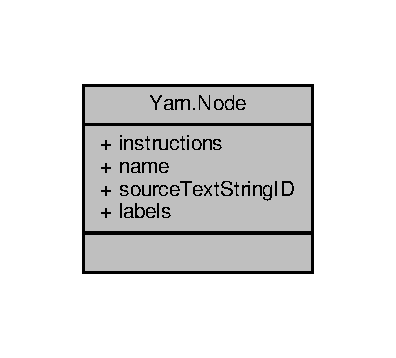
\includegraphics[width=190pt]{a00189}
\end{center}
\end{figure}
\begin{DoxyFields}{Class Members}
\hypertarget{a00040_a156723a9252b62d288ddf611939ea7c3}{List$<$ \hyperlink{a00058}{Instruction} $>$}\label{a00040_a156723a9252b62d288ddf611939ea7c3}
&
instructions&
\\
\hline

\hypertarget{a00040_a9afa49f4fbc72e806a0210cb4198f12e}{Dictionary$<$ string, int $>$}\label{a00040_a9afa49f4fbc72e806a0210cb4198f12e}
&
labels&
\\
\hline

\hypertarget{a00040_a107b0de3fcfc65e99913edc01b5ce9db}{string}\label{a00040_a107b0de3fcfc65e99913edc01b5ce9db}
&
name&
\\
\hline

\hypertarget{a00040_a09c6af5b50925d0876283b84281b3ed4}{string}\label{a00040_a09c6af5b50925d0876283b84281b3ed4}
&
source\-Text\-String\-I\-D&
\\
\hline

\end{DoxyFields}
\index{Yarn\-::\-Line@{Yarn\-::\-Line}}\label{a00180}
\hypertarget{a00040_a00180}{}
\subsubsection{struct Yarn\-:\-:Line}


Collaboration diagram for Yarn.\-Line\-:
\nopagebreak
\begin{figure}[H]
\begin{center}
\leavevmode
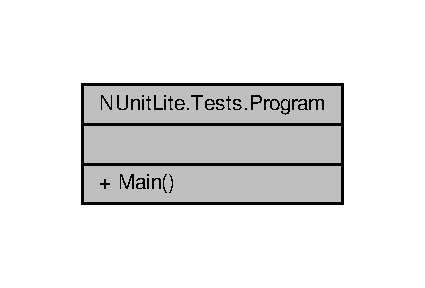
\includegraphics[width=136pt]{a00191}
\end{center}
\end{figure}
\begin{DoxyFields}{Class Members}
\hypertarget{a00040_a81d1f04bbb4cf6642d2bd685bda1da20}{string}\label{a00040_a81d1f04bbb4cf6642d2bd685bda1da20}
&
text&
\\
\hline

\end{DoxyFields}
\index{Yarn\-::\-Options@{Yarn\-::\-Options}}\label{a00182}
\hypertarget{a00040_a00182}{}
\subsubsection{struct Yarn\-:\-:Options}


Collaboration diagram for Yarn.\-Options\-:
\nopagebreak
\begin{figure}[H]
\begin{center}
\leavevmode
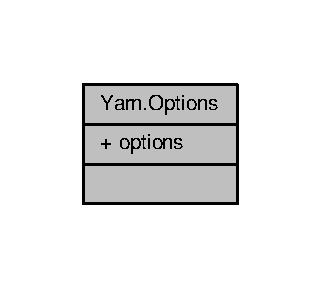
\includegraphics[width=154pt]{a00192}
\end{center}
\end{figure}
\begin{DoxyFields}{Class Members}
\hypertarget{a00040_ae8c616d923ceeeed192a9436c55d9917}{I\-List$<$ string $>$}\label{a00040_ae8c616d923ceeeed192a9436c55d9917}
&
options&
\\
\hline

\end{DoxyFields}
\index{Yarn\-::\-Command@{Yarn\-::\-Command}}\label{a00177}
\hypertarget{a00040_a00177}{}
\subsubsection{struct Yarn\-:\-:Command}


Collaboration diagram for Yarn.\-Command\-:
\nopagebreak
\begin{figure}[H]
\begin{center}
\leavevmode
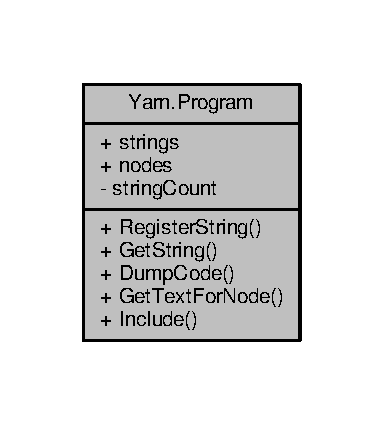
\includegraphics[width=164pt]{a00193}
\end{center}
\end{figure}
\begin{DoxyFields}{Class Members}
\hypertarget{a00040_a8564e5104566e145f5d917ec846444d9}{string}\label{a00040_a8564e5104566e145f5d917ec846444d9}
&
text&
\\
\hline

\end{DoxyFields}


\subsection{Enumeration Type Documentation}
\hypertarget{a00040_ad5dfb6ee68ca7469623ad3e459f98894}{\index{Yarn@{Yarn}!Byte\-Code@{Byte\-Code}}
\index{Byte\-Code@{Byte\-Code}!Yarn@{Yarn}}
\subsubsection[{Byte\-Code}]{\setlength{\rightskip}{0pt plus 5cm}enum {\bf Yarn.\-Byte\-Code}\hspace{0.3cm}{\ttfamily [package]}}}\label{a00040_ad5dfb6ee68ca7469623ad3e459f98894}
\begin{Desc}
\item[Enumerator]\par
\begin{description}
\index{Label@{Label}!Yarn@{Yarn}}\index{Yarn@{Yarn}!Label@{Label}}\item[{\em 
\hypertarget{a00040_ad5dfb6ee68ca7469623ad3e459f98894ab021df6aac4654c454f46c77646e745f}{Label}\label{a00040_ad5dfb6ee68ca7469623ad3e459f98894ab021df6aac4654c454f46c77646e745f}
}]\index{Jump\-To@{Jump\-To}!Yarn@{Yarn}}\index{Yarn@{Yarn}!Jump\-To@{Jump\-To}}\item[{\em 
\hypertarget{a00040_ad5dfb6ee68ca7469623ad3e459f98894acd664ebca0b52a8f2ece7d0767bacb49}{Jump\-To}\label{a00040_ad5dfb6ee68ca7469623ad3e459f98894acd664ebca0b52a8f2ece7d0767bacb49}
}]\index{Jump@{Jump}!Yarn@{Yarn}}\index{Yarn@{Yarn}!Jump@{Jump}}\item[{\em 
\hypertarget{a00040_ad5dfb6ee68ca7469623ad3e459f98894a101f693f72287a2819a364f64ca1c0ed}{Jump}\label{a00040_ad5dfb6ee68ca7469623ad3e459f98894a101f693f72287a2819a364f64ca1c0ed}
}]\index{Run\-Line@{Run\-Line}!Yarn@{Yarn}}\index{Yarn@{Yarn}!Run\-Line@{Run\-Line}}\item[{\em 
\hypertarget{a00040_ad5dfb6ee68ca7469623ad3e459f98894a005c6df9c6edea5516e29d96571fbbbc}{Run\-Line}\label{a00040_ad5dfb6ee68ca7469623ad3e459f98894a005c6df9c6edea5516e29d96571fbbbc}
}]\index{Run\-Command@{Run\-Command}!Yarn@{Yarn}}\index{Yarn@{Yarn}!Run\-Command@{Run\-Command}}\item[{\em 
\hypertarget{a00040_ad5dfb6ee68ca7469623ad3e459f98894a64d231d79e9f7640a4572f7ae75aa226}{Run\-Command}\label{a00040_ad5dfb6ee68ca7469623ad3e459f98894a64d231d79e9f7640a4572f7ae75aa226}
}]\index{Add\-Option@{Add\-Option}!Yarn@{Yarn}}\index{Yarn@{Yarn}!Add\-Option@{Add\-Option}}\item[{\em 
\hypertarget{a00040_ad5dfb6ee68ca7469623ad3e459f98894a0e6a6b9eb32a4d55f277d45eff74250d}{Add\-Option}\label{a00040_ad5dfb6ee68ca7469623ad3e459f98894a0e6a6b9eb32a4d55f277d45eff74250d}
}]\index{Show\-Options@{Show\-Options}!Yarn@{Yarn}}\index{Yarn@{Yarn}!Show\-Options@{Show\-Options}}\item[{\em 
\hypertarget{a00040_ad5dfb6ee68ca7469623ad3e459f98894a658963e1a47a5018fd1e6fbc2af804f7}{Show\-Options}\label{a00040_ad5dfb6ee68ca7469623ad3e459f98894a658963e1a47a5018fd1e6fbc2af804f7}
}]\index{Push\-String@{Push\-String}!Yarn@{Yarn}}\index{Yarn@{Yarn}!Push\-String@{Push\-String}}\item[{\em 
\hypertarget{a00040_ad5dfb6ee68ca7469623ad3e459f98894a3e7800d36ccb7bfe6c463bbe7db7e41a}{Push\-String}\label{a00040_ad5dfb6ee68ca7469623ad3e459f98894a3e7800d36ccb7bfe6c463bbe7db7e41a}
}]\index{Push\-Number@{Push\-Number}!Yarn@{Yarn}}\index{Yarn@{Yarn}!Push\-Number@{Push\-Number}}\item[{\em 
\hypertarget{a00040_ad5dfb6ee68ca7469623ad3e459f98894a29c8f5d9d5088ada190ccd9c21c31f33}{Push\-Number}\label{a00040_ad5dfb6ee68ca7469623ad3e459f98894a29c8f5d9d5088ada190ccd9c21c31f33}
}]\index{Push\-Bool@{Push\-Bool}!Yarn@{Yarn}}\index{Yarn@{Yarn}!Push\-Bool@{Push\-Bool}}\item[{\em 
\hypertarget{a00040_ad5dfb6ee68ca7469623ad3e459f98894af698d0b66ccf00f7d362c039949d1b80}{Push\-Bool}\label{a00040_ad5dfb6ee68ca7469623ad3e459f98894af698d0b66ccf00f7d362c039949d1b80}
}]\index{Push\-Null@{Push\-Null}!Yarn@{Yarn}}\index{Yarn@{Yarn}!Push\-Null@{Push\-Null}}\item[{\em 
\hypertarget{a00040_ad5dfb6ee68ca7469623ad3e459f98894acf728db6b8e47e735666156aec7ae755}{Push\-Null}\label{a00040_ad5dfb6ee68ca7469623ad3e459f98894acf728db6b8e47e735666156aec7ae755}
}]\index{Jump\-If\-False@{Jump\-If\-False}!Yarn@{Yarn}}\index{Yarn@{Yarn}!Jump\-If\-False@{Jump\-If\-False}}\item[{\em 
\hypertarget{a00040_ad5dfb6ee68ca7469623ad3e459f98894af8bbf32f00c942d974ade428e24b021f}{Jump\-If\-False}\label{a00040_ad5dfb6ee68ca7469623ad3e459f98894af8bbf32f00c942d974ade428e24b021f}
}]\index{Pop@{Pop}!Yarn@{Yarn}}\index{Yarn@{Yarn}!Pop@{Pop}}\item[{\em 
\hypertarget{a00040_ad5dfb6ee68ca7469623ad3e459f98894a0ae61bd0474e04c9f1195d4baa0213a0}{Pop}\label{a00040_ad5dfb6ee68ca7469623ad3e459f98894a0ae61bd0474e04c9f1195d4baa0213a0}
}]\index{Call\-Func@{Call\-Func}!Yarn@{Yarn}}\index{Yarn@{Yarn}!Call\-Func@{Call\-Func}}\item[{\em 
\hypertarget{a00040_ad5dfb6ee68ca7469623ad3e459f98894a3b5e7e8300dc6e4b78cb865c5b10f01a}{Call\-Func}\label{a00040_ad5dfb6ee68ca7469623ad3e459f98894a3b5e7e8300dc6e4b78cb865c5b10f01a}
}]\index{Push\-Variable@{Push\-Variable}!Yarn@{Yarn}}\index{Yarn@{Yarn}!Push\-Variable@{Push\-Variable}}\item[{\em 
\hypertarget{a00040_ad5dfb6ee68ca7469623ad3e459f98894ab8c46f65015a178516fadbb5ad6c2038}{Push\-Variable}\label{a00040_ad5dfb6ee68ca7469623ad3e459f98894ab8c46f65015a178516fadbb5ad6c2038}
}]\index{Store\-Variable@{Store\-Variable}!Yarn@{Yarn}}\index{Yarn@{Yarn}!Store\-Variable@{Store\-Variable}}\item[{\em 
\hypertarget{a00040_ad5dfb6ee68ca7469623ad3e459f98894a872dc050abaff4beb46e70dadd4088c2}{Store\-Variable}\label{a00040_ad5dfb6ee68ca7469623ad3e459f98894a872dc050abaff4beb46e70dadd4088c2}
}]\index{Stop@{Stop}!Yarn@{Yarn}}\index{Yarn@{Yarn}!Stop@{Stop}}\item[{\em 
\hypertarget{a00040_ad5dfb6ee68ca7469623ad3e459f98894a11a755d598c0c417f9a36758c3da7481}{Stop}\label{a00040_ad5dfb6ee68ca7469623ad3e459f98894a11a755d598c0c417f9a36758c3da7481}
}]\index{Run\-Node@{Run\-Node}!Yarn@{Yarn}}\index{Yarn@{Yarn}!Run\-Node@{Run\-Node}}\item[{\em 
\hypertarget{a00040_ad5dfb6ee68ca7469623ad3e459f98894ae956bcf888278c168ee9b106927ff6ac}{Run\-Node}\label{a00040_ad5dfb6ee68ca7469623ad3e459f98894ae956bcf888278c168ee9b106927ff6ac}
}]\end{description}
\end{Desc}

\begin{DoxyCode}
214                            \{
215         
216         \hyperlink{a00040_ad5dfb6ee68ca7469623ad3e459f98894ab021df6aac4654c454f46c77646e745f}{Label},             \textcolor{comment}{// opA = string: label name}
217         \hyperlink{a00040_ad5dfb6ee68ca7469623ad3e459f98894acd664ebca0b52a8f2ece7d0767bacb49}{JumpTo},               \textcolor{comment}{// opA = string: label name}
218         \hyperlink{a00040_ad5dfb6ee68ca7469623ad3e459f98894a101f693f72287a2819a364f64ca1c0ed}{Jump},               \textcolor{comment}{// peek string from stack and jump to that label}
219         \hyperlink{a00040_ad5dfb6ee68ca7469623ad3e459f98894a005c6df9c6edea5516e29d96571fbbbc}{RunLine},         \textcolor{comment}{// opA = int: string number}
220         \hyperlink{a00040_ad5dfb6ee68ca7469623ad3e459f98894a64d231d79e9f7640a4572f7ae75aa226}{RunCommand},           \textcolor{comment}{// opA = string: command text}
221         \hyperlink{a00040_ad5dfb6ee68ca7469623ad3e459f98894a0e6a6b9eb32a4d55f277d45eff74250d}{AddOption},         \textcolor{comment}{// opA = int: string number for option to add}
222         \hyperlink{a00040_ad5dfb6ee68ca7469623ad3e459f98894a658963e1a47a5018fd1e6fbc2af804f7}{ShowOptions},     \textcolor{comment}{// present the current list of options, then clear the list; most
       recently selected option will be on the top of the stack}
223         \hyperlink{a00040_ad5dfb6ee68ca7469623ad3e459f98894a3e7800d36ccb7bfe6c463bbe7db7e41a}{PushString},           \textcolor{comment}{// opA = int: string number in table; push string to stack}
224         \hyperlink{a00040_ad5dfb6ee68ca7469623ad3e459f98894a29c8f5d9d5088ada190ccd9c21c31f33}{PushNumber},           \textcolor{comment}{// opA = float: number to push to stack}
225         \hyperlink{a00040_ad5dfb6ee68ca7469623ad3e459f98894af698d0b66ccf00f7d362c039949d1b80}{PushBool},           \textcolor{comment}{// opA = int (0 or 1): bool to push to stack}
226         \hyperlink{a00040_ad5dfb6ee68ca7469623ad3e459f98894acf728db6b8e47e735666156aec7ae755}{PushNull},           \textcolor{comment}{// pushes a null value onto the stack}
227         \hyperlink{a00040_ad5dfb6ee68ca7469623ad3e459f98894af8bbf32f00c942d974ade428e24b021f}{JumpIfFalse},     \textcolor{comment}{// opA = string: label name if top of stack is not null, zero or false,
       jumps to that label}
228         \hyperlink{a00040_ad5dfb6ee68ca7469623ad3e459f98894a0ae61bd0474e04c9f1195d4baa0213a0}{Pop},             \textcolor{comment}{// discard top of stack}
229         \hyperlink{a00040_ad5dfb6ee68ca7469623ad3e459f98894a3b5e7e8300dc6e4b78cb865c5b10f01a}{CallFunc},           \textcolor{comment}{// opA = string; looks up function, pops as many arguments as needed,
       result is pushed to stack}
230         \hyperlink{a00040_ad5dfb6ee68ca7469623ad3e459f98894ab8c46f65015a178516fadbb5ad6c2038}{PushVariable},               \textcolor{comment}{// opA = name of variable to get value of and push to stack}
231         \hyperlink{a00040_ad5dfb6ee68ca7469623ad3e459f98894a872dc050abaff4beb46e70dadd4088c2}{StoreVariable},             \textcolor{comment}{// opA = name of variable to store top of stack in}
232         \hyperlink{a00040_ad5dfb6ee68ca7469623ad3e459f98894a11a755d598c0c417f9a36758c3da7481}{Stop},               \textcolor{comment}{// stops execution}
233         \hyperlink{a00040_ad5dfb6ee68ca7469623ad3e459f98894ae956bcf888278c168ee9b106927ff6ac}{RunNode}              \textcolor{comment}{// run the node whose name is at the top of the stack}
234 
235     \}
\end{DoxyCode}
\hypertarget{a00040_a301aa7c866593a5b625a8fc158bbeace}{\index{Yarn@{Yarn}!Token\-Type@{Token\-Type}}
\index{Token\-Type@{Token\-Type}!Yarn@{Yarn}}
\subsubsection[{Token\-Type}]{\setlength{\rightskip}{0pt plus 5cm}enum {\bf Yarn.\-Token\-Type}\hspace{0.3cm}{\ttfamily [package]}}}\label{a00040_a301aa7c866593a5b625a8fc158bbeace}
\begin{Desc}
\item[Enumerator]\par
\begin{description}
\index{Whitespace@{Whitespace}!Yarn@{Yarn}}\index{Yarn@{Yarn}!Whitespace@{Whitespace}}\item[{\em 
\hypertarget{a00040_a301aa7c866593a5b625a8fc158bbeaceace9a733c2ae3f8b704aec91f551b2bcc}{Whitespace}\label{a00040_a301aa7c866593a5b625a8fc158bbeaceace9a733c2ae3f8b704aec91f551b2bcc}
}]\index{Indent@{Indent}!Yarn@{Yarn}}\index{Yarn@{Yarn}!Indent@{Indent}}\item[{\em 
\hypertarget{a00040_a301aa7c866593a5b625a8fc158bbeacea497470e76a40fc53e14c0df9b4e4ec9f}{Indent}\label{a00040_a301aa7c866593a5b625a8fc158bbeacea497470e76a40fc53e14c0df9b4e4ec9f}
}]\index{Dedent@{Dedent}!Yarn@{Yarn}}\index{Yarn@{Yarn}!Dedent@{Dedent}}\item[{\em 
\hypertarget{a00040_a301aa7c866593a5b625a8fc158bbeacea675b39ecba872a6cf58d578781bf5216}{Dedent}\label{a00040_a301aa7c866593a5b625a8fc158bbeacea675b39ecba872a6cf58d578781bf5216}
}]\index{End\-Of\-Line@{End\-Of\-Line}!Yarn@{Yarn}}\index{Yarn@{Yarn}!End\-Of\-Line@{End\-Of\-Line}}\item[{\em 
\hypertarget{a00040_a301aa7c866593a5b625a8fc158bbeacea5d8c95ca9e91a87bd9c90b0f309fd740}{End\-Of\-Line}\label{a00040_a301aa7c866593a5b625a8fc158bbeacea5d8c95ca9e91a87bd9c90b0f309fd740}
}]\index{End\-Of\-Input@{End\-Of\-Input}!Yarn@{Yarn}}\index{Yarn@{Yarn}!End\-Of\-Input@{End\-Of\-Input}}\item[{\em 
\hypertarget{a00040_a301aa7c866593a5b625a8fc158bbeacea571dd25ea11480e6fe93f07a27059fbd}{End\-Of\-Input}\label{a00040_a301aa7c866593a5b625a8fc158bbeacea571dd25ea11480e6fe93f07a27059fbd}
}]\index{Number@{Number}!Yarn@{Yarn}}\index{Yarn@{Yarn}!Number@{Number}}\item[{\em 
\hypertarget{a00040_a301aa7c866593a5b625a8fc158bbeaceab2ee912b91d69b435159c7c3f6df7f5f}{Number}\label{a00040_a301aa7c866593a5b625a8fc158bbeaceab2ee912b91d69b435159c7c3f6df7f5f}
}]\index{String@{String}!Yarn@{Yarn}}\index{Yarn@{Yarn}!String@{String}}\item[{\em 
\hypertarget{a00040_a301aa7c866593a5b625a8fc158bbeacea27118326006d3829667a400ad23d5d98}{String}\label{a00040_a301aa7c866593a5b625a8fc158bbeacea27118326006d3829667a400ad23d5d98}
}]\index{Begin\-Command@{Begin\-Command}!Yarn@{Yarn}}\index{Yarn@{Yarn}!Begin\-Command@{Begin\-Command}}\item[{\em 
\hypertarget{a00040_a301aa7c866593a5b625a8fc158bbeacea2fb334b031e5462b88186810b5dba5ee}{Begin\-Command}\label{a00040_a301aa7c866593a5b625a8fc158bbeacea2fb334b031e5462b88186810b5dba5ee}
}]\index{End\-Command@{End\-Command}!Yarn@{Yarn}}\index{Yarn@{Yarn}!End\-Command@{End\-Command}}\item[{\em 
\hypertarget{a00040_a301aa7c866593a5b625a8fc158bbeacea6d879fc3833a8dc8742400a3c76b56fd}{End\-Command}\label{a00040_a301aa7c866593a5b625a8fc158bbeacea6d879fc3833a8dc8742400a3c76b56fd}
}]\index{Variable@{Variable}!Yarn@{Yarn}}\index{Yarn@{Yarn}!Variable@{Variable}}\item[{\em 
\hypertarget{a00040_a301aa7c866593a5b625a8fc158bbeacea47c14840d8e15331fa420b9b2f757cd9}{Variable}\label{a00040_a301aa7c866593a5b625a8fc158bbeacea47c14840d8e15331fa420b9b2f757cd9}
}]\index{Shortcut\-Option@{Shortcut\-Option}!Yarn@{Yarn}}\index{Yarn@{Yarn}!Shortcut\-Option@{Shortcut\-Option}}\item[{\em 
\hypertarget{a00040_a301aa7c866593a5b625a8fc158bbeacea07001155edc33437d76742b7ac124529}{Shortcut\-Option}\label{a00040_a301aa7c866593a5b625a8fc158bbeacea07001155edc33437d76742b7ac124529}
}]\index{Option\-Start@{Option\-Start}!Yarn@{Yarn}}\index{Yarn@{Yarn}!Option\-Start@{Option\-Start}}\item[{\em 
\hypertarget{a00040_a301aa7c866593a5b625a8fc158bbeaceaf6500edfd37e45de2894dc48866dca81}{Option\-Start}\label{a00040_a301aa7c866593a5b625a8fc158bbeaceaf6500edfd37e45de2894dc48866dca81}
}]\index{Option\-Delimit@{Option\-Delimit}!Yarn@{Yarn}}\index{Yarn@{Yarn}!Option\-Delimit@{Option\-Delimit}}\item[{\em 
\hypertarget{a00040_a301aa7c866593a5b625a8fc158bbeaceabbf373bbaabc962ed2d5f5cec1ebd49b}{Option\-Delimit}\label{a00040_a301aa7c866593a5b625a8fc158bbeaceabbf373bbaabc962ed2d5f5cec1ebd49b}
}]\index{Option\-End@{Option\-End}!Yarn@{Yarn}}\index{Yarn@{Yarn}!Option\-End@{Option\-End}}\item[{\em 
\hypertarget{a00040_a301aa7c866593a5b625a8fc158bbeacea2c617506a5bd9d900fd650a4bee0e626}{Option\-End}\label{a00040_a301aa7c866593a5b625a8fc158bbeacea2c617506a5bd9d900fd650a4bee0e626}
}]\index{If@{If}!Yarn@{Yarn}}\index{Yarn@{Yarn}!If@{If}}\item[{\em 
\hypertarget{a00040_a301aa7c866593a5b625a8fc158bbeacea786887572f6ef1c20f2d8177cb2f1639}{If}\label{a00040_a301aa7c866593a5b625a8fc158bbeacea786887572f6ef1c20f2d8177cb2f1639}
}]\index{Else\-If@{Else\-If}!Yarn@{Yarn}}\index{Yarn@{Yarn}!Else\-If@{Else\-If}}\item[{\em 
\hypertarget{a00040_a301aa7c866593a5b625a8fc158bbeaceaea5b66107aeb6829d789adefcfaac6eb}{Else\-If}\label{a00040_a301aa7c866593a5b625a8fc158bbeaceaea5b66107aeb6829d789adefcfaac6eb}
}]\index{Else@{Else}!Yarn@{Yarn}}\index{Yarn@{Yarn}!Else@{Else}}\item[{\em 
\hypertarget{a00040_a301aa7c866593a5b625a8fc158bbeacea6a0053231db40a4539b8f783a719a54a}{Else}\label{a00040_a301aa7c866593a5b625a8fc158bbeacea6a0053231db40a4539b8f783a719a54a}
}]\index{End\-If@{End\-If}!Yarn@{Yarn}}\index{Yarn@{Yarn}!End\-If@{End\-If}}\item[{\em 
\hypertarget{a00040_a301aa7c866593a5b625a8fc158bbeaceade360e1624063d8b9de7d2c411a960d8}{End\-If}\label{a00040_a301aa7c866593a5b625a8fc158bbeaceade360e1624063d8b9de7d2c411a960d8}
}]\index{Set@{Set}!Yarn@{Yarn}}\index{Yarn@{Yarn}!Set@{Set}}\item[{\em 
\hypertarget{a00040_a301aa7c866593a5b625a8fc158bbeacea5d5b78699e57104f2fa03bbdf7b9197b}{Set}\label{a00040_a301aa7c866593a5b625a8fc158bbeacea5d5b78699e57104f2fa03bbdf7b9197b}
}]\index{True@{True}!Yarn@{Yarn}}\index{Yarn@{Yarn}!True@{True}}\item[{\em 
\hypertarget{a00040_a301aa7c866593a5b625a8fc158bbeaceaf827cf462f62848df37c5e1e94a4da74}{True}\label{a00040_a301aa7c866593a5b625a8fc158bbeaceaf827cf462f62848df37c5e1e94a4da74}
}]\index{False@{False}!Yarn@{Yarn}}\index{Yarn@{Yarn}!False@{False}}\item[{\em 
\hypertarget{a00040_a301aa7c866593a5b625a8fc158bbeaceaf8320b26d30ab433c5a54546d21f414c}{False}\label{a00040_a301aa7c866593a5b625a8fc158bbeaceaf8320b26d30ab433c5a54546d21f414c}
}]\index{Null@{Null}!Yarn@{Yarn}}\index{Yarn@{Yarn}!Null@{Null}}\item[{\em 
\hypertarget{a00040_a301aa7c866593a5b625a8fc158bbeaceabbb93ef26e3c101ff11cdd21cab08a94}{Null}\label{a00040_a301aa7c866593a5b625a8fc158bbeaceabbb93ef26e3c101ff11cdd21cab08a94}
}]\index{Left\-Paren@{Left\-Paren}!Yarn@{Yarn}}\index{Yarn@{Yarn}!Left\-Paren@{Left\-Paren}}\item[{\em 
\hypertarget{a00040_a301aa7c866593a5b625a8fc158bbeaceaf02071a8b56c676adabcad98429fa14e}{Left\-Paren}\label{a00040_a301aa7c866593a5b625a8fc158bbeaceaf02071a8b56c676adabcad98429fa14e}
}]\index{Right\-Paren@{Right\-Paren}!Yarn@{Yarn}}\index{Yarn@{Yarn}!Right\-Paren@{Right\-Paren}}\item[{\em 
\hypertarget{a00040_a301aa7c866593a5b625a8fc158bbeacea2d7e137ea20e2c01ce105573d47ce525}{Right\-Paren}\label{a00040_a301aa7c866593a5b625a8fc158bbeacea2d7e137ea20e2c01ce105573d47ce525}
}]\index{Comma@{Comma}!Yarn@{Yarn}}\index{Yarn@{Yarn}!Comma@{Comma}}\item[{\em 
\hypertarget{a00040_a301aa7c866593a5b625a8fc158bbeacea58be47db9455679e6a44df2eff9c9fa6}{Comma}\label{a00040_a301aa7c866593a5b625a8fc158bbeacea58be47db9455679e6a44df2eff9c9fa6}
}]\index{Equal\-To@{Equal\-To}!Yarn@{Yarn}}\index{Yarn@{Yarn}!Equal\-To@{Equal\-To}}\item[{\em 
\hypertarget{a00040_a301aa7c866593a5b625a8fc158bbeacea0242c502bd906e05171e64bad31c7c21}{Equal\-To}\label{a00040_a301aa7c866593a5b625a8fc158bbeacea0242c502bd906e05171e64bad31c7c21}
}]\index{Greater\-Than@{Greater\-Than}!Yarn@{Yarn}}\index{Yarn@{Yarn}!Greater\-Than@{Greater\-Than}}\item[{\em 
\hypertarget{a00040_a301aa7c866593a5b625a8fc158bbeaceaf6d044fe1f01fb0c956b80099e2a3072}{Greater\-Than}\label{a00040_a301aa7c866593a5b625a8fc158bbeaceaf6d044fe1f01fb0c956b80099e2a3072}
}]\index{Greater\-Than\-Or\-Equal\-To@{Greater\-Than\-Or\-Equal\-To}!Yarn@{Yarn}}\index{Yarn@{Yarn}!Greater\-Than\-Or\-Equal\-To@{Greater\-Than\-Or\-Equal\-To}}\item[{\em 
\hypertarget{a00040_a301aa7c866593a5b625a8fc158bbeacea96b5d5dce523a30ceae47db080d8af48}{Greater\-Than\-Or\-Equal\-To}\label{a00040_a301aa7c866593a5b625a8fc158bbeacea96b5d5dce523a30ceae47db080d8af48}
}]\index{Less\-Than@{Less\-Than}!Yarn@{Yarn}}\index{Yarn@{Yarn}!Less\-Than@{Less\-Than}}\item[{\em 
\hypertarget{a00040_a301aa7c866593a5b625a8fc158bbeaceac6d9d7bb9939f62f01c80f8b1251501c}{Less\-Than}\label{a00040_a301aa7c866593a5b625a8fc158bbeaceac6d9d7bb9939f62f01c80f8b1251501c}
}]\index{Less\-Than\-Or\-Equal\-To@{Less\-Than\-Or\-Equal\-To}!Yarn@{Yarn}}\index{Yarn@{Yarn}!Less\-Than\-Or\-Equal\-To@{Less\-Than\-Or\-Equal\-To}}\item[{\em 
\hypertarget{a00040_a301aa7c866593a5b625a8fc158bbeacea67827f79b05c979b2378e9514bb7e741}{Less\-Than\-Or\-Equal\-To}\label{a00040_a301aa7c866593a5b625a8fc158bbeacea67827f79b05c979b2378e9514bb7e741}
}]\index{Not\-Equal\-To@{Not\-Equal\-To}!Yarn@{Yarn}}\index{Yarn@{Yarn}!Not\-Equal\-To@{Not\-Equal\-To}}\item[{\em 
\hypertarget{a00040_a301aa7c866593a5b625a8fc158bbeacea0961129d84d9d8f6aa4138a3e5022a1d}{Not\-Equal\-To}\label{a00040_a301aa7c866593a5b625a8fc158bbeacea0961129d84d9d8f6aa4138a3e5022a1d}
}]\index{Or@{Or}!Yarn@{Yarn}}\index{Yarn@{Yarn}!Or@{Or}}\item[{\em 
\hypertarget{a00040_a301aa7c866593a5b625a8fc158bbeacea3a2d5fe857d8f9541136a124c2edec6c}{Or}\label{a00040_a301aa7c866593a5b625a8fc158bbeacea3a2d5fe857d8f9541136a124c2edec6c}
}]\index{And@{And}!Yarn@{Yarn}}\index{Yarn@{Yarn}!And@{And}}\item[{\em 
\hypertarget{a00040_a301aa7c866593a5b625a8fc158bbeaceac33315685a0cba3ce53be378b3c7874b}{And}\label{a00040_a301aa7c866593a5b625a8fc158bbeaceac33315685a0cba3ce53be378b3c7874b}
}]\index{Xor@{Xor}!Yarn@{Yarn}}\index{Yarn@{Yarn}!Xor@{Xor}}\item[{\em 
\hypertarget{a00040_a301aa7c866593a5b625a8fc158bbeacea76feb79109026728a20736a8c6504548}{Xor}\label{a00040_a301aa7c866593a5b625a8fc158bbeacea76feb79109026728a20736a8c6504548}
}]\index{Not@{Not}!Yarn@{Yarn}}\index{Yarn@{Yarn}!Not@{Not}}\item[{\em 
\hypertarget{a00040_a301aa7c866593a5b625a8fc158bbeaceaa74c05d080620f087c4e523977230666}{Not}\label{a00040_a301aa7c866593a5b625a8fc158bbeaceaa74c05d080620f087c4e523977230666}
}]\index{Equal\-To\-Or\-Assign@{Equal\-To\-Or\-Assign}!Yarn@{Yarn}}\index{Yarn@{Yarn}!Equal\-To\-Or\-Assign@{Equal\-To\-Or\-Assign}}\item[{\em 
\hypertarget{a00040_a301aa7c866593a5b625a8fc158bbeacea9f086f3b58f1b290002de301d3a7ab24}{Equal\-To\-Or\-Assign}\label{a00040_a301aa7c866593a5b625a8fc158bbeacea9f086f3b58f1b290002de301d3a7ab24}
}]\index{Unary\-Minus@{Unary\-Minus}!Yarn@{Yarn}}\index{Yarn@{Yarn}!Unary\-Minus@{Unary\-Minus}}\item[{\em 
\hypertarget{a00040_a301aa7c866593a5b625a8fc158bbeacea87c80963dae5cd099e3a377e4d314b20}{Unary\-Minus}\label{a00040_a301aa7c866593a5b625a8fc158bbeacea87c80963dae5cd099e3a377e4d314b20}
}]\index{Add@{Add}!Yarn@{Yarn}}\index{Yarn@{Yarn}!Add@{Add}}\item[{\em 
\hypertarget{a00040_a301aa7c866593a5b625a8fc158bbeaceaec211f7c20af43e742bf2570c3cb84f9}{Add}\label{a00040_a301aa7c866593a5b625a8fc158bbeaceaec211f7c20af43e742bf2570c3cb84f9}
}]\index{Minus@{Minus}!Yarn@{Yarn}}\index{Yarn@{Yarn}!Minus@{Minus}}\item[{\em 
\hypertarget{a00040_a301aa7c866593a5b625a8fc158bbeacea453fb623e752c5993f65bc410fd74fe5}{Minus}\label{a00040_a301aa7c866593a5b625a8fc158bbeacea453fb623e752c5993f65bc410fd74fe5}
}]\index{Multiply@{Multiply}!Yarn@{Yarn}}\index{Yarn@{Yarn}!Multiply@{Multiply}}\item[{\em 
\hypertarget{a00040_a301aa7c866593a5b625a8fc158bbeaceae257376d913f3b53cbb4a9b19d770648}{Multiply}\label{a00040_a301aa7c866593a5b625a8fc158bbeaceae257376d913f3b53cbb4a9b19d770648}
}]\index{Divide@{Divide}!Yarn@{Yarn}}\index{Yarn@{Yarn}!Divide@{Divide}}\item[{\em 
\hypertarget{a00040_a301aa7c866593a5b625a8fc158bbeacea0b914e196182d02615487e9793ecff3d}{Divide}\label{a00040_a301aa7c866593a5b625a8fc158bbeacea0b914e196182d02615487e9793ecff3d}
}]\index{Add\-Assign@{Add\-Assign}!Yarn@{Yarn}}\index{Yarn@{Yarn}!Add\-Assign@{Add\-Assign}}\item[{\em 
\hypertarget{a00040_a301aa7c866593a5b625a8fc158bbeaceab055bb9ca4c2fabe4be4aa6e9e3278c6}{Add\-Assign}\label{a00040_a301aa7c866593a5b625a8fc158bbeaceab055bb9ca4c2fabe4be4aa6e9e3278c6}
}]\index{Minus\-Assign@{Minus\-Assign}!Yarn@{Yarn}}\index{Yarn@{Yarn}!Minus\-Assign@{Minus\-Assign}}\item[{\em 
\hypertarget{a00040_a301aa7c866593a5b625a8fc158bbeaceab05d460746c046306a3b74039a9977ba}{Minus\-Assign}\label{a00040_a301aa7c866593a5b625a8fc158bbeaceab05d460746c046306a3b74039a9977ba}
}]\index{Multiply\-Assign@{Multiply\-Assign}!Yarn@{Yarn}}\index{Yarn@{Yarn}!Multiply\-Assign@{Multiply\-Assign}}\item[{\em 
\hypertarget{a00040_a301aa7c866593a5b625a8fc158bbeacea7c3dfbd9bd6620d1cde7bbad4750a9c4}{Multiply\-Assign}\label{a00040_a301aa7c866593a5b625a8fc158bbeacea7c3dfbd9bd6620d1cde7bbad4750a9c4}
}]\index{Divide\-Assign@{Divide\-Assign}!Yarn@{Yarn}}\index{Yarn@{Yarn}!Divide\-Assign@{Divide\-Assign}}\item[{\em 
\hypertarget{a00040_a301aa7c866593a5b625a8fc158bbeacea60776f3f45a828ebfd062b8ad8118b38}{Divide\-Assign}\label{a00040_a301aa7c866593a5b625a8fc158bbeacea60776f3f45a828ebfd062b8ad8118b38}
}]\index{Comment@{Comment}!Yarn@{Yarn}}\index{Yarn@{Yarn}!Comment@{Comment}}\item[{\em 
\hypertarget{a00040_a301aa7c866593a5b625a8fc158bbeacea0be8406951cdfda82f00f79328cf4efc}{Comment}\label{a00040_a301aa7c866593a5b625a8fc158bbeacea0be8406951cdfda82f00f79328cf4efc}
}]\index{Identifier@{Identifier}!Yarn@{Yarn}}\index{Yarn@{Yarn}!Identifier@{Identifier}}\item[{\em 
\hypertarget{a00040_a301aa7c866593a5b625a8fc158bbeacea29ee5d1ebcc033234938a5234f1f2075}{Identifier}\label{a00040_a301aa7c866593a5b625a8fc158bbeacea29ee5d1ebcc033234938a5234f1f2075}
}]\index{Text@{Text}!Yarn@{Yarn}}\index{Yarn@{Yarn}!Text@{Text}}\item[{\em 
\hypertarget{a00040_a301aa7c866593a5b625a8fc158bbeacea9dffbf69ffba8bc38bc4e01abf4b1675}{Text}\label{a00040_a301aa7c866593a5b625a8fc158bbeacea9dffbf69ffba8bc38bc4e01abf4b1675}
}]\end{description}
\end{Desc}

\begin{DoxyCode}
79                             \{
80 
81 
82         
83         \textcolor{comment}{// Special tokens}
84         \hyperlink{a00040_a301aa7c866593a5b625a8fc158bbeaceace9a733c2ae3f8b704aec91f551b2bcc}{Whitespace},
85         \hyperlink{a00040_a301aa7c866593a5b625a8fc158bbeacea497470e76a40fc53e14c0df9b4e4ec9f}{Indent},
86         \hyperlink{a00040_a301aa7c866593a5b625a8fc158bbeacea675b39ecba872a6cf58d578781bf5216}{Dedent},
87         \hyperlink{a00040_a301aa7c866593a5b625a8fc158bbeacea5d8c95ca9e91a87bd9c90b0f309fd740}{EndOfLine},
88         \hyperlink{a00040_a301aa7c866593a5b625a8fc158bbeacea571dd25ea11480e6fe93f07a27059fbd}{EndOfInput},
89 
90         \textcolor{comment}{// Numbers. Everybody loves a number}
91         \hyperlink{a00151_a9d0536e3d8d9353112cfd292cc41b236ab2ee912b91d69b435159c7c3f6df7f5f}{Number},
92 
93         \textcolor{comment}{// Strings. Everybody also loves a string}
94         \hyperlink{a00151_a9d0536e3d8d9353112cfd292cc41b236a27118326006d3829667a400ad23d5d98}{String},
95 
96         \textcolor{comment}{// Command syntax ("<<foo>>")}
97         \hyperlink{a00040_a301aa7c866593a5b625a8fc158bbeacea2fb334b031e5462b88186810b5dba5ee}{BeginCommand},
98         \hyperlink{a00040_a301aa7c866593a5b625a8fc158bbeacea6d879fc3833a8dc8742400a3c76b56fd}{EndCommand},
99 
100         \textcolor{comment}{// Variables ("$foo")}
101         \hyperlink{a00040_a301aa7c866593a5b625a8fc158bbeacea47c14840d8e15331fa420b9b2f757cd9}{Variable},
102 
103         \textcolor{comment}{// Shortcut syntax ("->")}
104         \hyperlink{a00040_a301aa7c866593a5b625a8fc158bbeacea07001155edc33437d76742b7ac124529}{ShortcutOption},
105 
106         \textcolor{comment}{// Option syntax ("[[Let's go here|Destination]]")}
107         \hyperlink{a00040_a301aa7c866593a5b625a8fc158bbeaceaf6500edfd37e45de2894dc48866dca81}{OptionStart}, \textcolor{comment}{// [[}
108         \hyperlink{a00040_a301aa7c866593a5b625a8fc158bbeaceabbf373bbaabc962ed2d5f5cec1ebd49b}{OptionDelimit}, \textcolor{comment}{// |}
109         \hyperlink{a00040_a301aa7c866593a5b625a8fc158bbeacea2c617506a5bd9d900fd650a4bee0e626}{OptionEnd}, \textcolor{comment}{// ]]}
110 
111         \textcolor{comment}{// Command types (specially recognised command word)}
112         \hyperlink{a00040_a301aa7c866593a5b625a8fc158bbeacea786887572f6ef1c20f2d8177cb2f1639}{If},
113         \hyperlink{a00040_a301aa7c866593a5b625a8fc158bbeaceaea5b66107aeb6829d789adefcfaac6eb}{ElseIf},
114         \hyperlink{a00040_a301aa7c866593a5b625a8fc158bbeacea6a0053231db40a4539b8f783a719a54a}{Else},
115         \hyperlink{a00040_a301aa7c866593a5b625a8fc158bbeaceade360e1624063d8b9de7d2c411a960d8}{EndIf},
116         \hyperlink{a00040_a301aa7c866593a5b625a8fc158bbeacea5d5b78699e57104f2fa03bbdf7b9197b}{Set},
117 
118         \textcolor{comment}{// Boolean values}
119         \hyperlink{a00151_a9d0536e3d8d9353112cfd292cc41b236af827cf462f62848df37c5e1e94a4da74}{True},
120         \hyperlink{a00151_a9d0536e3d8d9353112cfd292cc41b236af8320b26d30ab433c5a54546d21f414c}{False},
121 
122         \textcolor{comment}{// The null value}
123         \hyperlink{a00151_a9d0536e3d8d9353112cfd292cc41b236abbb93ef26e3c101ff11cdd21cab08a94}{Null},
124 
125         \textcolor{comment}{// Parentheses}
126         \hyperlink{a00040_a301aa7c866593a5b625a8fc158bbeaceaf02071a8b56c676adabcad98429fa14e}{LeftParen},
127         \hyperlink{a00040_a301aa7c866593a5b625a8fc158bbeacea2d7e137ea20e2c01ce105573d47ce525}{RightParen},
128 
129         \textcolor{comment}{// Parameter delimiters}
130         \hyperlink{a00151_a9d0536e3d8d9353112cfd292cc41b236a58be47db9455679e6a44df2eff9c9fa6}{Comma},
131 
132         \textcolor{comment}{// Operators}
133         \hyperlink{a00040_a301aa7c866593a5b625a8fc158bbeacea0242c502bd906e05171e64bad31c7c21}{EqualTo}, \textcolor{comment}{// ==, eq, is}
134         \hyperlink{a00040_a301aa7c866593a5b625a8fc158bbeaceaf6d044fe1f01fb0c956b80099e2a3072}{GreaterThan}, \textcolor{comment}{// >, gt}
135         \hyperlink{a00040_a301aa7c866593a5b625a8fc158bbeacea96b5d5dce523a30ceae47db080d8af48}{GreaterThanOrEqualTo}, \textcolor{comment}{// >=, gte}
136         \hyperlink{a00040_a301aa7c866593a5b625a8fc158bbeaceac6d9d7bb9939f62f01c80f8b1251501c}{LessThan}, \textcolor{comment}{// <, lt}
137         \hyperlink{a00040_a301aa7c866593a5b625a8fc158bbeacea67827f79b05c979b2378e9514bb7e741}{LessThanOrEqualTo}, \textcolor{comment}{// <=, lte}
138         \hyperlink{a00040_a301aa7c866593a5b625a8fc158bbeacea0961129d84d9d8f6aa4138a3e5022a1d}{NotEqualTo}, \textcolor{comment}{// !=, neq}
139 
140         \textcolor{comment}{// Logical operators}
141         \hyperlink{a00040_a301aa7c866593a5b625a8fc158bbeacea3a2d5fe857d8f9541136a124c2edec6c}{Or}, \textcolor{comment}{// ||, or}
142         \hyperlink{a00040_a301aa7c866593a5b625a8fc158bbeaceac33315685a0cba3ce53be378b3c7874b}{And}, \textcolor{comment}{// &&, and}
143         \hyperlink{a00040_a301aa7c866593a5b625a8fc158bbeacea76feb79109026728a20736a8c6504548}{Xor}, \textcolor{comment}{// ^, xor}
144         \hyperlink{a00040_a301aa7c866593a5b625a8fc158bbeaceaa74c05d080620f087c4e523977230666}{Not}, \textcolor{comment}{// !, not}
145 
146 
147         \textcolor{comment}{// this guy's special because '=' can mean either 'equal to' }
148         \textcolor{comment}{// or 'becomes' depending on context}
149         \hyperlink{a00040_a301aa7c866593a5b625a8fc158bbeacea9f086f3b58f1b290002de301d3a7ab24}{EqualToOrAssign}, \textcolor{comment}{// =, to}
150 
151         \hyperlink{a00040_a301aa7c866593a5b625a8fc158bbeacea87c80963dae5cd099e3a377e4d314b20}{UnaryMinus}, \textcolor{comment}{// -; this is differentiated from Minus }
152                     \textcolor{comment}{// when parsing expressions}
153 
154         \hyperlink{a00040_a301aa7c866593a5b625a8fc158bbeaceaec211f7c20af43e742bf2570c3cb84f9}{Add}, \textcolor{comment}{// +}
155         \hyperlink{a00040_a301aa7c866593a5b625a8fc158bbeacea453fb623e752c5993f65bc410fd74fe5}{Minus}, \textcolor{comment}{// -}
156         \hyperlink{a00040_a301aa7c866593a5b625a8fc158bbeaceae257376d913f3b53cbb4a9b19d770648}{Multiply}, \textcolor{comment}{// *}
157         \hyperlink{a00040_a301aa7c866593a5b625a8fc158bbeacea0b914e196182d02615487e9793ecff3d}{Divide}, \textcolor{comment}{// /}
158         
159         \hyperlink{a00040_a301aa7c866593a5b625a8fc158bbeaceab055bb9ca4c2fabe4be4aa6e9e3278c6}{AddAssign}, \textcolor{comment}{// +=}
160         \hyperlink{a00040_a301aa7c866593a5b625a8fc158bbeaceab05d460746c046306a3b74039a9977ba}{MinusAssign}, \textcolor{comment}{// -=}
161         \hyperlink{a00040_a301aa7c866593a5b625a8fc158bbeacea7c3dfbd9bd6620d1cde7bbad4750a9c4}{MultiplyAssign}, \textcolor{comment}{// *=}
162         \hyperlink{a00040_a301aa7c866593a5b625a8fc158bbeacea60776f3f45a828ebfd062b8ad8118b38}{DivideAssign}, \textcolor{comment}{// /=}
163 
164         \hyperlink{a00040_a301aa7c866593a5b625a8fc158bbeacea0be8406951cdfda82f00f79328cf4efc}{Comment}, \textcolor{comment}{// a run of text that we ignore}
165 
166         \hyperlink{a00040_a301aa7c866593a5b625a8fc158bbeacea29ee5d1ebcc033234938a5234f1f2075}{Identifier}, \textcolor{comment}{// a single word (used for functions)}
167 
168         \hyperlink{a00040_a301aa7c866593a5b625a8fc158bbeacea9dffbf69ffba8bc38bc4e01abf4b1675}{Text} \textcolor{comment}{// a run of text until we hit other syntax}
169     \}
\end{DoxyCode}


\subsection{Function Documentation}
\hypertarget{a00040_ae0be2e5cf13d5779816102439e61ff1a}{\index{Yarn@{Yarn}!Function@{Function}}
\index{Function@{Function}!Yarn@{Yarn}}
\subsubsection[{Function}]{\setlength{\rightskip}{0pt plus 5cm}delegate void Yarn.\-Function (
\begin{DoxyParamCaption}
\item[{params Value\mbox{[}$\,$\mbox{]}}]{parameters}
\end{DoxyParamCaption}
)}}\label{a00040_ae0be2e5cf13d5779816102439e61ff1a}
\hypertarget{a00040_a1e50031b945a3a2afafee6f590730568}{\index{Yarn@{Yarn}!Logger@{Logger}}
\index{Logger@{Logger}!Yarn@{Yarn}}
\subsubsection[{Logger}]{\setlength{\rightskip}{0pt plus 5cm}delegate void Yarn.\-Logger (
\begin{DoxyParamCaption}
\item[{string}]{message}
\end{DoxyParamCaption}
)}}\label{a00040_a1e50031b945a3a2afafee6f590730568}
\hypertarget{a00040_a39866cbb03c03a35805d598b5d4ad553}{\index{Yarn@{Yarn}!Option\-Chooser@{Option\-Chooser}}
\index{Option\-Chooser@{Option\-Chooser}!Yarn@{Yarn}}
\subsubsection[{Option\-Chooser}]{\setlength{\rightskip}{0pt plus 5cm}delegate void Yarn.\-Option\-Chooser (
\begin{DoxyParamCaption}
\item[{int}]{selected\-Option\-Index}
\end{DoxyParamCaption}
)}}\label{a00040_a39866cbb03c03a35805d598b5d4ad553}
\hypertarget{a00040_a5177bf74fbfe7303fac9d8236c2e514b}{\index{Yarn@{Yarn}!Returning\-Function@{Returning\-Function}}
\index{Returning\-Function@{Returning\-Function}!Yarn@{Yarn}}
\subsubsection[{Returning\-Function}]{\setlength{\rightskip}{0pt plus 5cm}delegate Object Yarn.\-Returning\-Function (
\begin{DoxyParamCaption}
\item[{params Value\mbox{[}$\,$\mbox{]}}]{parameters}
\end{DoxyParamCaption}
)}}\label{a00040_a5177bf74fbfe7303fac9d8236c2e514b}

\hypertarget{a00041}{\section{Csv\-Helper.\-Configuration.\-Csv\-Class\-Map$<$ T $>$ Class Template Reference}
\label{a00041}\index{Csv\-Helper.\-Configuration.\-Csv\-Class\-Map$<$ T $>$@{Csv\-Helper.\-Configuration.\-Csv\-Class\-Map$<$ T $>$}}
}


Maps class properties to C\-S\-V fields.  




Inheritance diagram for Csv\-Helper.\-Configuration.\-Csv\-Class\-Map$<$ T $>$\-:
\nopagebreak
\begin{figure}[H]
\begin{center}
\leavevmode
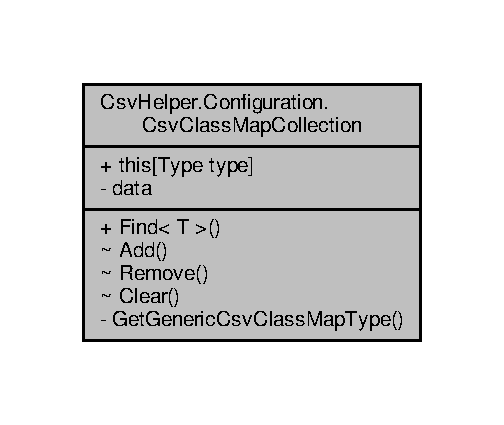
\includegraphics[width=232pt]{d1/d98/a00407}
\end{center}
\end{figure}


Collaboration diagram for Csv\-Helper.\-Configuration.\-Csv\-Class\-Map$<$ T $>$\-:
\nopagebreak
\begin{figure}[H]
\begin{center}
\leavevmode
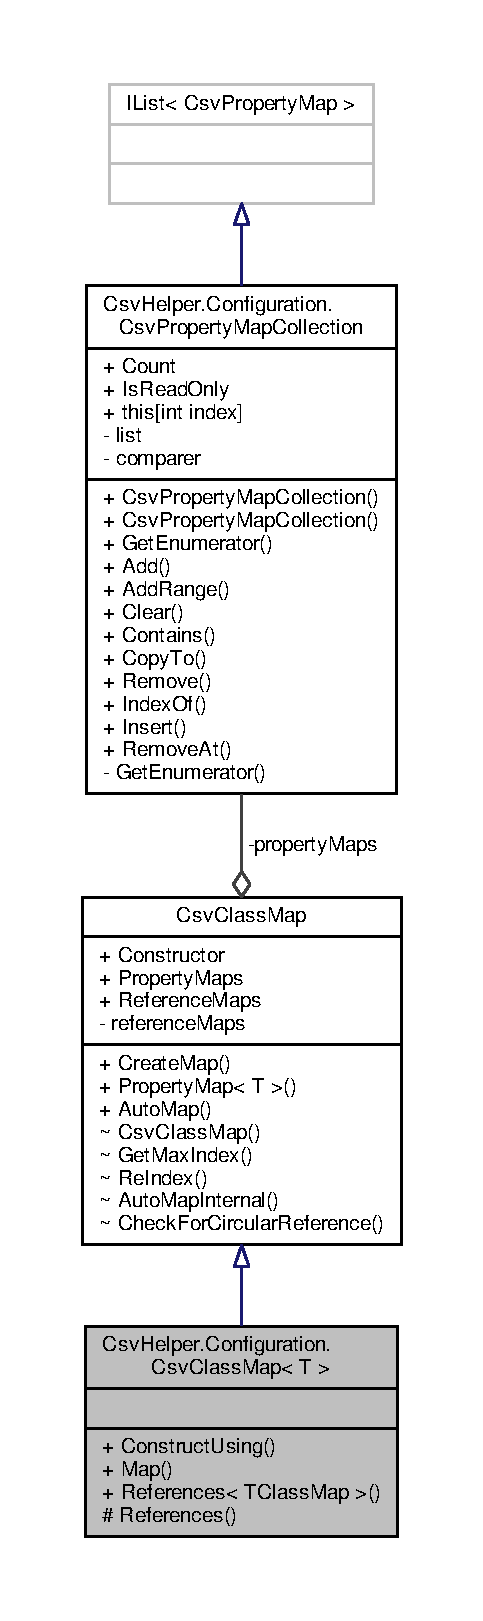
\includegraphics[height=550pt]{dd/dea/a00408}
\end{center}
\end{figure}
\subsection*{Public Member Functions}
\begin{DoxyCompactItemize}
\item 
virtual void \hyperlink{a00041_a983d792ae80f888958037eea306b143a}{Construct\-Using} (Expression$<$ Func$<$ T $>$$>$ expression)
\begin{DoxyCompactList}\small\item\em Constructs the row object using the given expression. \end{DoxyCompactList}\item 
virtual \hyperlink{a00050}{Csv\-Property\-Map} \hyperlink{a00041_aa3395a5f657f0dd7c8fe6a0fbf5a03cb}{Map} (Expression$<$ Func$<$ T, object $>$$>$ expression)
\begin{DoxyCompactList}\small\item\em Maps a property to a C\-S\-V field. \end{DoxyCompactList}\item 
virtual \hyperlink{a00055}{Csv\-Property\-Reference\-Map} \hyperlink{a00041_a20365b78c96ac29e3261bcde30e0d746}{References$<$ T\-Class\-Map $>$} (Expression$<$ Func$<$ T, object $>$$>$ expression, params object\mbox{[}$\,$\mbox{]} constructor\-Args)
\begin{DoxyCompactList}\small\item\em Maps a property to another class map. \end{DoxyCompactList}\item 
virtual void \hyperlink{a00040_a83de9d28160d0d3da1e017df554a9481}{Create\-Map} ()
\begin{DoxyCompactList}\small\item\em Called to create the mappings. \end{DoxyCompactList}\item 
virtual \hyperlink{a00050}{Csv\-Property\-Map} \hyperlink{a00040_abab2b5cd5a290fd5d17116430b084420}{Property\-Map$<$ T $>$} (Expression$<$ Func$<$ T, object $>$$>$ expression)
\begin{DoxyCompactList}\small\item\em Gets the property map for the given property expression. \end{DoxyCompactList}\item 
virtual void \hyperlink{a00040_aec2097b09baaaac45171f91592af439d}{Auto\-Map} (bool ignore\-References=false, bool prefix\-Reference\-Headers=false)
\begin{DoxyCompactList}\small\item\em Auto maps all properties for the given type. If a property is mapped again it will override the existing map. \end{DoxyCompactList}\end{DoxyCompactItemize}
\subsection*{Protected Member Functions}
\begin{DoxyCompactItemize}
\item 
virtual \hyperlink{a00055}{Csv\-Property\-Reference\-Map} \hyperlink{a00041_a68caeee244e978110a2acae6d3042fc3}{References} (Type type, Expression$<$ Func$<$ T, object $>$$>$ expression, params object\mbox{[}$\,$\mbox{]} constructor\-Args)
\begin{DoxyCompactList}\small\item\em Maps a property to another class map. \end{DoxyCompactList}\end{DoxyCompactItemize}
\subsection*{Package Functions}
\begin{DoxyCompactItemize}
\item 
int \hyperlink{a00040_a708c455aa7f78a26b55dafc46a587ec3}{Get\-Max\-Index} ()
\begin{DoxyCompactList}\small\item\em Get the largest index for the properties and references. \end{DoxyCompactList}\item 
int \hyperlink{a00040_ac6c1e8ae1d049bd0ef09e7c2d99fbe55}{Re\-Index} (int index\-Start=0)
\begin{DoxyCompactList}\small\item\em Resets the indexes based on the given start index. \end{DoxyCompactList}\end{DoxyCompactItemize}
\subsection*{Static Package Functions}
\begin{DoxyCompactItemize}
\item 
static void \hyperlink{a00040_a16b5bb84064e86c2b319348d8a42693d}{Auto\-Map\-Internal} (\hyperlink{a00040}{Csv\-Class\-Map} map, bool ignore\-References, bool prefix\-Reference\-Headers, Linked\-List$<$ Type $>$ map\-Parents, int index\-Start=0)
\begin{DoxyCompactList}\small\item\em Auto maps the given map and checks for circular references as it goes. \end{DoxyCompactList}\item 
static bool \hyperlink{a00040_a4b2f3fc2e0670d17566b4705b7b622aa}{Check\-For\-Circular\-Reference} (Type type, Linked\-List$<$ Type $>$ map\-Parents)
\begin{DoxyCompactList}\small\item\em Checks for circular references. \end{DoxyCompactList}\end{DoxyCompactItemize}
\subsection*{Properties}
\begin{DoxyCompactItemize}
\item 
virtual New\-Expression \hyperlink{a00040_ae8038b36db7584ef1a73852fcc46404b}{Constructor}\hspace{0.3cm}{\ttfamily  \mbox{[}get, set\mbox{]}}
\begin{DoxyCompactList}\small\item\em Gets the constructor expression. \end{DoxyCompactList}\item 
virtual \hyperlink{a00051}{Csv\-Property\-Map\-Collection} \hyperlink{a00040_a9580e897abcba144f3101eb983348e25}{Property\-Maps}\hspace{0.3cm}{\ttfamily  \mbox{[}get\mbox{]}}
\begin{DoxyCompactList}\small\item\em The class property mappings. \end{DoxyCompactList}\item 
virtual List\\*
$<$ \hyperlink{a00055}{Csv\-Property\-Reference\-Map} $>$ \hyperlink{a00040_a6dfbf8f743b16d2ec83edef865ea2d9e}{Reference\-Maps}\hspace{0.3cm}{\ttfamily  \mbox{[}get\mbox{]}}
\begin{DoxyCompactList}\small\item\em The class property reference mappings. \end{DoxyCompactList}\end{DoxyCompactItemize}


\subsection{Detailed Description}
Maps class properties to C\-S\-V fields. 


\begin{DoxyTemplParams}{Template Parameters}
{\em T} & The Type of class to map.\\
\hline
\end{DoxyTemplParams}


\subsection{Member Function Documentation}
\hypertarget{a00040_aec2097b09baaaac45171f91592af439d}{\index{Csv\-Helper\-::\-Configuration\-::\-Csv\-Class\-Map$<$ T $>$@{Csv\-Helper\-::\-Configuration\-::\-Csv\-Class\-Map$<$ T $>$}!Auto\-Map@{Auto\-Map}}
\index{Auto\-Map@{Auto\-Map}!CsvHelper::Configuration::CsvClassMap< T >@{Csv\-Helper\-::\-Configuration\-::\-Csv\-Class\-Map$<$ T $>$}}
\subsubsection[{Auto\-Map}]{\setlength{\rightskip}{0pt plus 5cm}virtual void Csv\-Helper.\-Configuration.\-Csv\-Class\-Map.\-Auto\-Map (
\begin{DoxyParamCaption}
\item[{bool}]{ignore\-References = {\ttfamily false}, }
\item[{bool}]{prefix\-Reference\-Headers = {\ttfamily false}}
\end{DoxyParamCaption}
)\hspace{0.3cm}{\ttfamily [virtual]}, {\ttfamily [inherited]}}}\label{a00040_aec2097b09baaaac45171f91592af439d}


Auto maps all properties for the given type. If a property is mapped again it will override the existing map. 


\begin{DoxyParams}{Parameters}
{\em ignore\-References} & A value indicating if references should be ignored when auto mapping. True to ignore references, otherwise false.\\
\hline
{\em prefix\-Reference\-Headers} & A value indicating if headers of reference properties should get prefixed by the parent property name. True to prefix, otherwise false.\\
\hline
\end{DoxyParams}

\begin{DoxyCode}
93         \{
94             var mapParents = \textcolor{keyword}{new} LinkedList<Type>();
95             \hyperlink{a00040_a16b5bb84064e86c2b319348d8a42693d}{AutoMapInternal}( \textcolor{keyword}{this}, ignoreReferences, prefixReferenceHeaders, mapParents );
96         \}
\end{DoxyCode}
\hypertarget{a00040_a16b5bb84064e86c2b319348d8a42693d}{\index{Csv\-Helper\-::\-Configuration\-::\-Csv\-Class\-Map$<$ T $>$@{Csv\-Helper\-::\-Configuration\-::\-Csv\-Class\-Map$<$ T $>$}!Auto\-Map\-Internal@{Auto\-Map\-Internal}}
\index{Auto\-Map\-Internal@{Auto\-Map\-Internal}!CsvHelper::Configuration::CsvClassMap< T >@{Csv\-Helper\-::\-Configuration\-::\-Csv\-Class\-Map$<$ T $>$}}
\subsubsection[{Auto\-Map\-Internal}]{\setlength{\rightskip}{0pt plus 5cm}static void Csv\-Helper.\-Configuration.\-Csv\-Class\-Map.\-Auto\-Map\-Internal (
\begin{DoxyParamCaption}
\item[{{\bf Csv\-Class\-Map}}]{map, }
\item[{bool}]{ignore\-References, }
\item[{bool}]{prefix\-Reference\-Headers, }
\item[{Linked\-List$<$ Type $>$}]{map\-Parents, }
\item[{int}]{index\-Start = {\ttfamily 0}}
\end{DoxyParamCaption}
)\hspace{0.3cm}{\ttfamily [static]}, {\ttfamily [package]}, {\ttfamily [inherited]}}}\label{a00040_a16b5bb84064e86c2b319348d8a42693d}


Auto maps the given map and checks for circular references as it goes. 


\begin{DoxyParams}{Parameters}
{\em map} & The map to auto map.\\
\hline
{\em ignore\-References} & A value indicating if references should be ignored when auto mapping. True to ignore references, otherwise false.\\
\hline
{\em prefix\-Reference\-Headers} & A value indicating if headers of reference properties should get prefixed by the parent property name. True to prefix, otherwise false.\\
\hline
{\em map\-Parents} & The list of parents for the map.\\
\hline
\end{DoxyParams}

\begin{DoxyCode}
154         \{
155             var type = map.GetType().GetTypeInfo().BaseType.GetGenericArguments()[0];
156             \textcolor{keywordflow}{if}( typeof( IEnumerable ).IsAssignableFrom( type ) )
157             \{
158                 \textcolor{keywordflow}{throw} \textcolor{keyword}{new} CsvConfigurationException( \textcolor{stringliteral}{"Types that inherit IEnumerable cannot be auto mapped.
       "} +
159                                                      \textcolor{stringliteral}{"Did you accidentally call GetRecord or WriteRecord
       which "} +
160                                                      \textcolor{stringliteral}{"acts on a single record instead of calling GetRecords
       or "} +
161                                                      \textcolor{stringliteral}{"WriteRecords which acts on a list of records?"} );
162             \}
163 
164             var properties = type.GetProperties( BindingFlags.Instance | BindingFlags.Public );
165             \textcolor{keywordflow}{foreach}( var property \textcolor{keywordflow}{in} properties )
166             \{
167                 var typeConverterType = TypeConverterFactory.GetConverter( property.PropertyType ).GetType(
      );
168                 \textcolor{keywordflow}{if}( typeConverterType == typeof( \hyperlink{a00078}{EnumerableConverter} ) )
169                 \{
170                     \textcolor{comment}{// The IEnumerable converter just throws an exception so skip it.}
171                     \textcolor{keywordflow}{continue};
172                 \}
173 
174                 var isDefaultConverter = typeConverterType == typeof( 
      \hyperlink{a00068}{DefaultTypeConverter} );
175                 var hasDefaultConstructor = property.PropertyType.GetConstructor( \textcolor{keyword}{new} Type[0] ) != null;
176                 \textcolor{keywordflow}{if}( isDefaultConverter && hasDefaultConstructor )
177                 \{
178                     \textcolor{keywordflow}{if}( ignoreReferences )
179                     \{
180                         \textcolor{keywordflow}{continue};
181                     \}
182 
183                     \textcolor{comment}{// If the type is not one covered by our type converters}
184                     \textcolor{comment}{// and it has a parameterless constructor, create a}
185                     \textcolor{comment}{// reference map for it.}
186                     \textcolor{keywordflow}{if}( \hyperlink{a00040_a4b2f3fc2e0670d17566b4705b7b622aa}{CheckForCircularReference}( property.PropertyType, 
      mapParents ) )
187                     \{
188                         \textcolor{keywordflow}{continue};
189                     \}
190 
191                     mapParents.AddLast( type );
192                     var refMapType = typeof( DefaultCsvClassMap<> ).MakeGenericType( property.PropertyType 
      );
193                     var refMap = (\hyperlink{a00040_affc5ae8f2b0406d496bcbdf246da6210}{CsvClassMap})ReflectionHelper.CreateInstance( refMapType );
194                     \hyperlink{a00040_a16b5bb84064e86c2b319348d8a42693d}{AutoMapInternal}( refMap, \textcolor{keyword}{false}, prefixReferenceHeaders, mapParents, map.
      GetMaxIndex() + 1 );
195 
196                     \textcolor{keywordflow}{if}( refMap.PropertyMaps.Count > 0 || refMap.ReferenceMaps.Count > 0 )
197                     \{
198                         var referenceMap = \textcolor{keyword}{new} CsvPropertyReferenceMap( property, refMap );
199                         \textcolor{keywordflow}{if}( prefixReferenceHeaders )
200                         \{
201                             referenceMap.Prefix();
202                         \}
203 
204                         map.ReferenceMaps.Add( referenceMap );
205                     \}
206                 \}
207                 \textcolor{keywordflow}{else}
208                 \{
209                     var propertyMap = \textcolor{keyword}{new} CsvPropertyMap( property );
210                     propertyMap.Data.Index = map.GetMaxIndex() + 1;
211                     \textcolor{keywordflow}{if}( propertyMap.Data.TypeConverter.CanConvertFrom( typeof( \textcolor{keywordtype}{string} ) ) ||
212                         propertyMap.Data.TypeConverter.CanConvertTo( typeof( \textcolor{keywordtype}{string} ) ) && !
      isDefaultConverter )
213                     \{
214                         \textcolor{comment}{// Only add the property map if it can be converted later on.}
215                         \textcolor{comment}{// If the property will use the default converter, don't add it because}
216                         \textcolor{comment}{// we don't want the .ToString() value to be used when auto mapping.}
217                         map.PropertyMaps.Add( propertyMap );
218                     \}
219                 \}
220             \}
221 
222             map.ReIndex( indexStart );
223         \}
\end{DoxyCode}
\hypertarget{a00040_a4b2f3fc2e0670d17566b4705b7b622aa}{\index{Csv\-Helper\-::\-Configuration\-::\-Csv\-Class\-Map$<$ T $>$@{Csv\-Helper\-::\-Configuration\-::\-Csv\-Class\-Map$<$ T $>$}!Check\-For\-Circular\-Reference@{Check\-For\-Circular\-Reference}}
\index{Check\-For\-Circular\-Reference@{Check\-For\-Circular\-Reference}!CsvHelper::Configuration::CsvClassMap< T >@{Csv\-Helper\-::\-Configuration\-::\-Csv\-Class\-Map$<$ T $>$}}
\subsubsection[{Check\-For\-Circular\-Reference}]{\setlength{\rightskip}{0pt plus 5cm}static bool Csv\-Helper.\-Configuration.\-Csv\-Class\-Map.\-Check\-For\-Circular\-Reference (
\begin{DoxyParamCaption}
\item[{Type}]{type, }
\item[{Linked\-List$<$ Type $>$}]{map\-Parents}
\end{DoxyParamCaption}
)\hspace{0.3cm}{\ttfamily [static]}, {\ttfamily [package]}, {\ttfamily [inherited]}}}\label{a00040_a4b2f3fc2e0670d17566b4705b7b622aa}


Checks for circular references. 


\begin{DoxyParams}{Parameters}
{\em type} & The type to check for.\\
\hline
{\em map\-Parents} & The list of parents to check against.\\
\hline
\end{DoxyParams}
\begin{DoxyReturn}{Returns}
A value indicating if a circular reference was found. True if a circular reference was found, otherwise false.
\end{DoxyReturn}

\begin{DoxyCode}
233         \{
234             \textcolor{keywordflow}{if}( mapParents.Count == 0 )
235             \{
236                 \textcolor{keywordflow}{return} \textcolor{keyword}{false};
237             \}
238 
239             var node = mapParents.Last;
240             \textcolor{keywordflow}{while}( \textcolor{keyword}{true} )
241             \{
242                 \textcolor{keywordflow}{if}( node.Value == type )
243                 \{
244                     \textcolor{keywordflow}{return} \textcolor{keyword}{true};
245                 \}
246 
247                 node = node.Previous;
248                 \textcolor{keywordflow}{if}( node == null )
249                 \{
250                     \textcolor{keywordflow}{break};
251                 \}
252             \}
253 
254             \textcolor{keywordflow}{return} \textcolor{keyword}{false};
255         \}
\end{DoxyCode}
\hypertarget{a00041_a983d792ae80f888958037eea306b143a}{\index{Csv\-Helper\-::\-Configuration\-::\-Csv\-Class\-Map$<$ T $>$@{Csv\-Helper\-::\-Configuration\-::\-Csv\-Class\-Map$<$ T $>$}!Construct\-Using@{Construct\-Using}}
\index{Construct\-Using@{Construct\-Using}!CsvHelper::Configuration::CsvClassMap< T >@{Csv\-Helper\-::\-Configuration\-::\-Csv\-Class\-Map$<$ T $>$}}
\subsubsection[{Construct\-Using}]{\setlength{\rightskip}{0pt plus 5cm}virtual void {\bf Csv\-Helper.\-Configuration.\-Csv\-Class\-Map}$<$ T $>$.Construct\-Using (
\begin{DoxyParamCaption}
\item[{Expression$<$ Func$<$ T $>$$>$}]{expression}
\end{DoxyParamCaption}
)\hspace{0.3cm}{\ttfamily [virtual]}}}\label{a00041_a983d792ae80f888958037eea306b143a}


Constructs the row object using the given expression. 


\begin{DoxyParams}{Parameters}
{\em expression} & The expression.\\
\hline
\end{DoxyParams}

\begin{DoxyCode}
27         \{
28             \hyperlink{a00040_ae8038b36db7584ef1a73852fcc46404b}{Constructor} = ReflectionHelper.GetConstructor( expression );
29         \}
\end{DoxyCode}
\hypertarget{a00040_a83de9d28160d0d3da1e017df554a9481}{\index{Csv\-Helper\-::\-Configuration\-::\-Csv\-Class\-Map$<$ T $>$@{Csv\-Helper\-::\-Configuration\-::\-Csv\-Class\-Map$<$ T $>$}!Create\-Map@{Create\-Map}}
\index{Create\-Map@{Create\-Map}!CsvHelper::Configuration::CsvClassMap< T >@{Csv\-Helper\-::\-Configuration\-::\-Csv\-Class\-Map$<$ T $>$}}
\subsubsection[{Create\-Map}]{\setlength{\rightskip}{0pt plus 5cm}virtual void Csv\-Helper.\-Configuration.\-Csv\-Class\-Map.\-Create\-Map (
\begin{DoxyParamCaption}
{}
\end{DoxyParamCaption}
)\hspace{0.3cm}{\ttfamily [virtual]}, {\ttfamily [inherited]}}}\label{a00040_a83de9d28160d0d3da1e017df554a9481}


Called to create the mappings. 


\begin{DoxyCode}
28 \{\}
\end{DoxyCode}
\hypertarget{a00040_a708c455aa7f78a26b55dafc46a587ec3}{\index{Csv\-Helper\-::\-Configuration\-::\-Csv\-Class\-Map$<$ T $>$@{Csv\-Helper\-::\-Configuration\-::\-Csv\-Class\-Map$<$ T $>$}!Get\-Max\-Index@{Get\-Max\-Index}}
\index{Get\-Max\-Index@{Get\-Max\-Index}!CsvHelper::Configuration::CsvClassMap< T >@{Csv\-Helper\-::\-Configuration\-::\-Csv\-Class\-Map$<$ T $>$}}
\subsubsection[{Get\-Max\-Index}]{\setlength{\rightskip}{0pt plus 5cm}int Csv\-Helper.\-Configuration.\-Csv\-Class\-Map.\-Get\-Max\-Index (
\begin{DoxyParamCaption}
{}
\end{DoxyParamCaption}
)\hspace{0.3cm}{\ttfamily [package]}, {\ttfamily [inherited]}}}\label{a00040_a708c455aa7f78a26b55dafc46a587ec3}


Get the largest index for the properties and references. 

\begin{DoxyReturn}{Returns}
The max index.
\end{DoxyReturn}

\begin{DoxyCode}
104         \{
105             \textcolor{keywordflow}{if}( \hyperlink{a00040_a9580e897abcba144f3101eb983348e25}{PropertyMaps}.\hyperlink{a00051_a45cac3a36ac638d4d4b723b7ceb93b5c}{Count} == 0 && \hyperlink{a00040_a6dfbf8f743b16d2ec83edef865ea2d9e}{ReferenceMaps}.Count == 0 )
106             \{
107                 \textcolor{keywordflow}{return} -1;
108             \}
109 
110             var indexes = \textcolor{keyword}{new} List<int>();
111             \textcolor{keywordflow}{if}( \hyperlink{a00040_a9580e897abcba144f3101eb983348e25}{PropertyMaps}.\hyperlink{a00051_a45cac3a36ac638d4d4b723b7ceb93b5c}{Count} > 0 )
112             \{
113                 indexes.Add( PropertyMaps.Max( pm => pm.Data.Index ) );
114             \}
115             indexes.AddRange( ReferenceMaps.Select( referenceMap => referenceMap.GetMaxIndex() ) );
116 
117             \textcolor{keywordflow}{return} indexes.Max();
118         \}
\end{DoxyCode}
\hypertarget{a00041_aa3395a5f657f0dd7c8fe6a0fbf5a03cb}{\index{Csv\-Helper\-::\-Configuration\-::\-Csv\-Class\-Map$<$ T $>$@{Csv\-Helper\-::\-Configuration\-::\-Csv\-Class\-Map$<$ T $>$}!Map@{Map}}
\index{Map@{Map}!CsvHelper::Configuration::CsvClassMap< T >@{Csv\-Helper\-::\-Configuration\-::\-Csv\-Class\-Map$<$ T $>$}}
\subsubsection[{Map}]{\setlength{\rightskip}{0pt plus 5cm}virtual {\bf Csv\-Property\-Map} {\bf Csv\-Helper.\-Configuration.\-Csv\-Class\-Map}$<$ T $>$.Map (
\begin{DoxyParamCaption}
\item[{Expression$<$ Func$<$ T, object $>$$>$}]{expression}
\end{DoxyParamCaption}
)\hspace{0.3cm}{\ttfamily [virtual]}}}\label{a00041_aa3395a5f657f0dd7c8fe6a0fbf5a03cb}


Maps a property to a C\-S\-V field. 


\begin{DoxyParams}{Parameters}
{\em expression} & The property to map.\\
\hline
\end{DoxyParams}
\begin{DoxyReturn}{Returns}
The property mapping.
\end{DoxyReturn}

\begin{DoxyCode}
37         \{
38             var \textcolor{keyword}{property} = ReflectionHelper.GetProperty( expression );
39 
40             var existingMap = PropertyMaps.SingleOrDefault( m =>
41                 m.Data.Property == \textcolor{keyword}{property}
42                 || m.Data.Property.Name == property.Name
43                 && ( m.Data.Property.DeclaringType.GetTypeInfo().IsAssignableFrom( property.DeclaringType.
      GetTypeInfo() ) || property.DeclaringType.IsAssignableFrom( m.Data.Property.DeclaringType ) ) );
44             \textcolor{keywordflow}{if}( existingMap != null )
45             \{
46                 \textcolor{keywordflow}{return} existingMap;
47             \}
48 
49             var propertyMap = \textcolor{keyword}{new} CsvPropertyMap( property );
50             propertyMap.Data.Index = \hyperlink{a00040_a708c455aa7f78a26b55dafc46a587ec3}{GetMaxIndex}() + 1;
51             PropertyMaps.Add( propertyMap );
52 
53             \textcolor{keywordflow}{return} propertyMap;
54         \}
\end{DoxyCode}
\hypertarget{a00040_abab2b5cd5a290fd5d17116430b084420}{\index{Csv\-Helper\-::\-Configuration\-::\-Csv\-Class\-Map$<$ T $>$@{Csv\-Helper\-::\-Configuration\-::\-Csv\-Class\-Map$<$ T $>$}!Property\-Map$<$ T $>$@{Property\-Map$<$ T $>$}}
\index{Property\-Map$<$ T $>$@{Property\-Map$<$ T $>$}!CsvHelper::Configuration::CsvClassMap< T >@{Csv\-Helper\-::\-Configuration\-::\-Csv\-Class\-Map$<$ T $>$}}
\subsubsection[{Property\-Map$<$ T $>$}]{\setlength{\rightskip}{0pt plus 5cm}virtual {\bf Csv\-Property\-Map} Csv\-Helper.\-Configuration.\-Csv\-Class\-Map.\-Property\-Map$<$ T $>$ (
\begin{DoxyParamCaption}
\item[{Expression$<$ Func$<$ T, object $>$$>$}]{expression}
\end{DoxyParamCaption}
)\hspace{0.3cm}{\ttfamily [virtual]}, {\ttfamily [inherited]}}}\label{a00040_abab2b5cd5a290fd5d17116430b084420}


Gets the property map for the given property expression. 


\begin{DoxyTemplParams}{Template Parameters}
{\em T} & The type of the class the property belongs to.\\
\hline
\end{DoxyTemplParams}

\begin{DoxyParams}{Parameters}
{\em expression} & The property expression.\\
\hline
\end{DoxyParams}
\begin{DoxyReturn}{Returns}
The \hyperlink{a00050}{Csv\-Property\-Map} for the given expression.
\end{DoxyReturn}

\begin{DoxyCode}
64         \{
65             var \textcolor{keyword}{property} = ReflectionHelper.GetProperty( expression );
66 
67             var existingMap = PropertyMaps.SingleOrDefault( m =>
68                 m.Data.Property == \textcolor{keyword}{property}
69                 || m.Data.Property.Name == property.Name
70                 && ( m.Data.Property.DeclaringType.IsAssignableFrom( property.DeclaringType ) || property.
      DeclaringType.IsAssignableFrom( m.Data.Property.DeclaringType ) ) );
71             \textcolor{keywordflow}{if}( existingMap != null )
72             \{
73                 \textcolor{keywordflow}{return} existingMap;
74             \}
75 
76             var propertyMap = \textcolor{keyword}{new} CsvPropertyMap( property );
77             propertyMap.Data.Index = \hyperlink{a00040_a708c455aa7f78a26b55dafc46a587ec3}{GetMaxIndex}() + 1;
78             PropertyMaps.Add( propertyMap );
79 
80             \textcolor{keywordflow}{return} propertyMap;
81         \}
\end{DoxyCode}
\hypertarget{a00041_a68caeee244e978110a2acae6d3042fc3}{\index{Csv\-Helper\-::\-Configuration\-::\-Csv\-Class\-Map$<$ T $>$@{Csv\-Helper\-::\-Configuration\-::\-Csv\-Class\-Map$<$ T $>$}!References@{References}}
\index{References@{References}!CsvHelper::Configuration::CsvClassMap< T >@{Csv\-Helper\-::\-Configuration\-::\-Csv\-Class\-Map$<$ T $>$}}
\subsubsection[{References}]{\setlength{\rightskip}{0pt plus 5cm}virtual {\bf Csv\-Property\-Reference\-Map} {\bf Csv\-Helper.\-Configuration.\-Csv\-Class\-Map}$<$ T $>$.References (
\begin{DoxyParamCaption}
\item[{Type}]{type, }
\item[{Expression$<$ Func$<$ T, object $>$$>$}]{expression, }
\item[{params object\mbox{[}$\,$\mbox{]}}]{constructor\-Args}
\end{DoxyParamCaption}
)\hspace{0.3cm}{\ttfamily [protected]}, {\ttfamily [virtual]}}}\label{a00041_a68caeee244e978110a2acae6d3042fc3}


Maps a property to another class map. 


\begin{DoxyParams}{Parameters}
{\em type} & The type.\\
\hline
{\em expression} & The expression.\\
\hline
{\em constructor\-Args} & Constructor arguments used to create the reference map.\\
\hline
\end{DoxyParams}
\begin{DoxyReturn}{Returns}
The reference mapping for the property
\end{DoxyReturn}

\begin{DoxyCode}
94         \{
95             var \textcolor{keyword}{property} = ReflectionHelper.GetProperty( expression );
96             var existingMap = ReferenceMaps.SingleOrDefault( m =>
97                 m.Data.Property == \textcolor{keyword}{property}
98                 || m.Data.Property.Name == property.Name
99                 && ( m.Data.Property.DeclaringType.IsAssignableFrom( property.DeclaringType ) || property.
      DeclaringType.IsAssignableFrom( m.Data.Property.DeclaringType ) ) );
100             \textcolor{keywordflow}{if}( existingMap != null )
101             \{
102                 \textcolor{keywordflow}{return} existingMap;
103             \}
104 
105             var map = (\hyperlink{a00040_affc5ae8f2b0406d496bcbdf246da6210}{CsvClassMap})ReflectionHelper.CreateInstance( type, constructorArgs );
106             map.CreateMap();
107             map.ReIndex( \hyperlink{a00040_a708c455aa7f78a26b55dafc46a587ec3}{GetMaxIndex}() + 1 );
108             var reference = \textcolor{keyword}{new} CsvPropertyReferenceMap( property, map );
109             ReferenceMaps.Add( reference );
110 
111             \textcolor{keywordflow}{return} reference;
112         \}
\end{DoxyCode}
\hypertarget{a00041_a20365b78c96ac29e3261bcde30e0d746}{\index{Csv\-Helper\-::\-Configuration\-::\-Csv\-Class\-Map$<$ T $>$@{Csv\-Helper\-::\-Configuration\-::\-Csv\-Class\-Map$<$ T $>$}!References$<$ T\-Class\-Map $>$@{References$<$ T\-Class\-Map $>$}}
\index{References$<$ T\-Class\-Map $>$@{References$<$ T\-Class\-Map $>$}!CsvHelper::Configuration::CsvClassMap< T >@{Csv\-Helper\-::\-Configuration\-::\-Csv\-Class\-Map$<$ T $>$}}
\subsubsection[{References$<$ T\-Class\-Map $>$}]{\setlength{\rightskip}{0pt plus 5cm}virtual {\bf Csv\-Property\-Reference\-Map} {\bf Csv\-Helper.\-Configuration.\-Csv\-Class\-Map}$<$ T $>$.{\bf References}$<$ T\-Class\-Map $>$ (
\begin{DoxyParamCaption}
\item[{Expression$<$ Func$<$ T, object $>$$>$}]{expression, }
\item[{params object\mbox{[}$\,$\mbox{]}}]{constructor\-Args}
\end{DoxyParamCaption}
)\hspace{0.3cm}{\ttfamily [virtual]}}}\label{a00041_a20365b78c96ac29e3261bcde30e0d746}


Maps a property to another class map. 


\begin{DoxyTemplParams}{Template Parameters}
{\em T\-Class\-Map} & The type of the class map.\\
\hline
\end{DoxyTemplParams}

\begin{DoxyParams}{Parameters}
{\em expression} & The expression.\\
\hline
{\em constructor\-Args} & Constructor arguments used to create the reference map.\\
\hline
\end{DoxyParams}
\begin{DoxyReturn}{Returns}
The reference mapping for the property.
\end{DoxyReturn}
\begin{Desc}
\item[Type Constraints]\begin{description}
\item[{\em T\-Class\-Map} : {\em Csv\-Class\-Map}]\end{description}
\end{Desc}

\begin{DoxyCode}
63                                                                                                            
                                                           : \hyperlink{a00040_affc5ae8f2b0406d496bcbdf246da6210}{CsvClassMap}
64         \{
65             var \textcolor{keyword}{property} = ReflectionHelper.GetProperty( expression );
66 
67             var existingMap = ReferenceMaps.SingleOrDefault( m =>
68                 m.Data.Property == \textcolor{keyword}{property}
69                 || m.Data.Property.Name == property.Name
70                 && ( m.Data.Property.DeclaringType.IsAssignableFrom( property.DeclaringType ) || property.
      DeclaringType.IsAssignableFrom( m.Data.Property.DeclaringType ) ) );
71             \textcolor{keywordflow}{if}( existingMap != null )
72             \{
73                 \textcolor{keywordflow}{return} existingMap;
74             \}
75 
76             var map = ReflectionHelper.CreateInstance<TClassMap>( constructorArgs );
77             map.CreateMap();
78             map.ReIndex( \hyperlink{a00040_a708c455aa7f78a26b55dafc46a587ec3}{GetMaxIndex}() + 1 );
79             var reference = \textcolor{keyword}{new} CsvPropertyReferenceMap( property, map );
80             ReferenceMaps.Add( reference );
81 
82             \textcolor{keywordflow}{return} reference;
83         \}
\end{DoxyCode}
\hypertarget{a00040_ac6c1e8ae1d049bd0ef09e7c2d99fbe55}{\index{Csv\-Helper\-::\-Configuration\-::\-Csv\-Class\-Map$<$ T $>$@{Csv\-Helper\-::\-Configuration\-::\-Csv\-Class\-Map$<$ T $>$}!Re\-Index@{Re\-Index}}
\index{Re\-Index@{Re\-Index}!CsvHelper::Configuration::CsvClassMap< T >@{Csv\-Helper\-::\-Configuration\-::\-Csv\-Class\-Map$<$ T $>$}}
\subsubsection[{Re\-Index}]{\setlength{\rightskip}{0pt plus 5cm}int Csv\-Helper.\-Configuration.\-Csv\-Class\-Map.\-Re\-Index (
\begin{DoxyParamCaption}
\item[{int}]{index\-Start = {\ttfamily 0}}
\end{DoxyParamCaption}
)\hspace{0.3cm}{\ttfamily [package]}, {\ttfamily [inherited]}}}\label{a00040_ac6c1e8ae1d049bd0ef09e7c2d99fbe55}


Resets the indexes based on the given start index. 


\begin{DoxyParams}{Parameters}
{\em index\-Start} & The index start.\\
\hline
\end{DoxyParams}
\begin{DoxyReturn}{Returns}
The last index + 1.
\end{DoxyReturn}

\begin{DoxyCode}
126         \{
127             \textcolor{keywordflow}{foreach}( var propertyMap \textcolor{keywordflow}{in} \hyperlink{a00040_a9580e897abcba144f3101eb983348e25}{PropertyMaps} )
128             \{
129                 \textcolor{keywordflow}{if}( !propertyMap.Data.IsIndexSet )
130                 \{
131                     propertyMap.Data.Index = indexStart + propertyMap.Data.Index;
132                 \}
133             \}
134 
135             \textcolor{keywordflow}{foreach}( var referenceMap \textcolor{keywordflow}{in} \hyperlink{a00040_a6dfbf8f743b16d2ec83edef865ea2d9e}{ReferenceMaps} )
136             \{
137                 indexStart = referenceMap.Data.Mapping.ReIndex( indexStart );
138             \}
139 
140             \textcolor{keywordflow}{return} indexStart;
141         \}
\end{DoxyCode}


\subsection{Property Documentation}
\hypertarget{a00040_ae8038b36db7584ef1a73852fcc46404b}{\index{Csv\-Helper\-::\-Configuration\-::\-Csv\-Class\-Map$<$ T $>$@{Csv\-Helper\-::\-Configuration\-::\-Csv\-Class\-Map$<$ T $>$}!Constructor@{Constructor}}
\index{Constructor@{Constructor}!CsvHelper::Configuration::CsvClassMap< T >@{Csv\-Helper\-::\-Configuration\-::\-Csv\-Class\-Map$<$ T $>$}}
\subsubsection[{Constructor}]{\setlength{\rightskip}{0pt plus 5cm}virtual New\-Expression Csv\-Helper.\-Configuration.\-Csv\-Class\-Map.\-Constructor\hspace{0.3cm}{\ttfamily [get]}, {\ttfamily [set]}, {\ttfamily [inherited]}}}\label{a00040_ae8038b36db7584ef1a73852fcc46404b}


Gets the constructor expression. 

\hypertarget{a00040_a9580e897abcba144f3101eb983348e25}{\index{Csv\-Helper\-::\-Configuration\-::\-Csv\-Class\-Map$<$ T $>$@{Csv\-Helper\-::\-Configuration\-::\-Csv\-Class\-Map$<$ T $>$}!Property\-Maps@{Property\-Maps}}
\index{Property\-Maps@{Property\-Maps}!CsvHelper::Configuration::CsvClassMap< T >@{Csv\-Helper\-::\-Configuration\-::\-Csv\-Class\-Map$<$ T $>$}}
\subsubsection[{Property\-Maps}]{\setlength{\rightskip}{0pt plus 5cm}virtual {\bf Csv\-Property\-Map\-Collection} Csv\-Helper.\-Configuration.\-Csv\-Class\-Map.\-Property\-Maps\hspace{0.3cm}{\ttfamily [get]}, {\ttfamily [inherited]}}}\label{a00040_a9580e897abcba144f3101eb983348e25}


The class property mappings. 

\hypertarget{a00040_a6dfbf8f743b16d2ec83edef865ea2d9e}{\index{Csv\-Helper\-::\-Configuration\-::\-Csv\-Class\-Map$<$ T $>$@{Csv\-Helper\-::\-Configuration\-::\-Csv\-Class\-Map$<$ T $>$}!Reference\-Maps@{Reference\-Maps}}
\index{Reference\-Maps@{Reference\-Maps}!CsvHelper::Configuration::CsvClassMap< T >@{Csv\-Helper\-::\-Configuration\-::\-Csv\-Class\-Map$<$ T $>$}}
\subsubsection[{Reference\-Maps}]{\setlength{\rightskip}{0pt plus 5cm}virtual List$<${\bf Csv\-Property\-Reference\-Map}$>$ Csv\-Helper.\-Configuration.\-Csv\-Class\-Map.\-Reference\-Maps\hspace{0.3cm}{\ttfamily [get]}, {\ttfamily [inherited]}}}\label{a00040_a6dfbf8f743b16d2ec83edef865ea2d9e}


The class property reference mappings. 



The documentation for this class was generated from the following file\-:\begin{DoxyCompactItemize}
\item 
packages/\-Csv\-Helper.\-2.\-16.\-0.\-0/src/\-Csv\-Helper/\-Configuration/\hyperlink{a00183}{Csv\-Class\-Map`1.\-cs}\end{DoxyCompactItemize}

\hypertarget{a00042}{\section{Yarn.\-Dialogue.\-Command\-Result Class Reference}
\label{a00042}\index{Yarn.\-Dialogue.\-Command\-Result@{Yarn.\-Dialogue.\-Command\-Result}}
}


The client should run a command (it's up to them to parse the string)  




Inheritance diagram for Yarn.\-Dialogue.\-Command\-Result\-:
\nopagebreak
\begin{figure}[H]
\begin{center}
\leavevmode
\includegraphics[width=234pt]{a00602}
\end{center}
\end{figure}


Collaboration diagram for Yarn.\-Dialogue.\-Command\-Result\-:
\nopagebreak
\begin{figure}[H]
\begin{center}
\leavevmode
\includegraphics[width=259pt]{a00603}
\end{center}
\end{figure}
\subsection*{Public Member Functions}
\begin{DoxyCompactItemize}
\item 
\hyperlink{a00042_a1a553422394fb0c854d1184985f993bb}{Command\-Result} (string text)
\end{DoxyCompactItemize}
\subsection*{Public Attributes}
\begin{DoxyCompactItemize}
\item 
\hyperlink{a00041_a00355}{Command} \hyperlink{a00042_a420ca0984d6e5c33bb761654305c592e}{command}
\end{DoxyCompactItemize}


\subsection{Detailed Description}
The client should run a command (it's up to them to parse the string) 

Definition at line 148 of file Dialogue.\-cs.



\subsection{Constructor \& Destructor Documentation}
\hypertarget{a00042_a1a553422394fb0c854d1184985f993bb}{\index{Yarn\-::\-Dialogue\-::\-Command\-Result@{Yarn\-::\-Dialogue\-::\-Command\-Result}!Command\-Result@{Command\-Result}}
\index{Command\-Result@{Command\-Result}!Yarn::Dialogue::CommandResult@{Yarn\-::\-Dialogue\-::\-Command\-Result}}
\subsubsection[{Command\-Result}]{\setlength{\rightskip}{0pt plus 5cm}Yarn.\-Dialogue.\-Command\-Result.\-Command\-Result (
\begin{DoxyParamCaption}
\item[{string}]{text}
\end{DoxyParamCaption}
)}}\label{a00042_a1a553422394fb0c854d1184985f993bb}


Definition at line 151 of file Dialogue.\-cs.



References Yarn.\-Dialogue.\-Command\-Result.\-command.


\begin{DoxyCode}
151                                                \{
152                 var \hyperlink{a00042_a420ca0984d6e5c33bb761654305c592e}{command} = \textcolor{keyword}{new} Command();
153                 command.text = text;
154                 this.command = \hyperlink{a00042_a420ca0984d6e5c33bb761654305c592e}{command};
155             \}
\end{DoxyCode}


\subsection{Member Data Documentation}
\hypertarget{a00042_a420ca0984d6e5c33bb761654305c592e}{\index{Yarn\-::\-Dialogue\-::\-Command\-Result@{Yarn\-::\-Dialogue\-::\-Command\-Result}!command@{command}}
\index{command@{command}!Yarn::Dialogue::CommandResult@{Yarn\-::\-Dialogue\-::\-Command\-Result}}
\subsubsection[{command}]{\setlength{\rightskip}{0pt plus 5cm}{\bf Command} Yarn.\-Dialogue.\-Command\-Result.\-command}}\label{a00042_a420ca0984d6e5c33bb761654305c592e}


Definition at line 149 of file Dialogue.\-cs.



Referenced by Yarn.\-Dialogue.\-Command\-Result.\-Command\-Result().



The documentation for this class was generated from the following file\-:\begin{DoxyCompactItemize}
\item 
Yarn\-Spinner/\hyperlink{a00290}{Dialogue.\-cs}\end{DoxyCompactItemize}

\hypertarget{a00043}{\section{Yarn.\-Parser.\-Block Class Reference}
\label{a00043}\index{Yarn.\-Parser.\-Block@{Yarn.\-Parser.\-Block}}
}


Inheritance diagram for Yarn.\-Parser.\-Block\-:
\nopagebreak
\begin{figure}[H]
\begin{center}
\leavevmode
\includegraphics[width=176pt]{a00672}
\end{center}
\end{figure}


Collaboration diagram for Yarn.\-Parser.\-Block\-:
\nopagebreak
\begin{figure}[H]
\begin{center}
\leavevmode
\includegraphics[width=254pt]{a00673}
\end{center}
\end{figure}
\subsection*{Public Member Functions}
\begin{DoxyCompactItemize}
\item 
string \hyperlink{a00148_a054f36c80d5eeacd569a8859f599af67}{Tags\-To\-String} (int indent\-Level)
\item 
override string \hyperlink{a00148_a18c67cb16090d0889bb9d6c8c6c565f8}{To\-String} ()
\end{DoxyCompactItemize}
\subsection*{Package Functions}
\begin{DoxyCompactItemize}
\item 
\hyperlink{a00043_a943abeb93be783da7ff6ca595b6a34e7}{Block} (\hyperlink{a00148}{Parse\-Node} \hyperlink{a00148_af313a82103fcc2ff5a177dbb06b92f7b}{parent}, \hyperlink{a00149}{Parser} p)
\item 
override string \hyperlink{a00043_aaaacfc4e3ff2871fa5e2fb75e48636de}{Print\-Tree} (int indent\-Level)
\item 
\hyperlink{a00138}{Node} \hyperlink{a00148_a580e520a29444fc23ac3660cbe514a09}{Node\-Parent} ()
\end{DoxyCompactItemize}
\subsection*{Static Package Functions}
\begin{DoxyCompactItemize}
\item 
static bool \hyperlink{a00043_a7fa97243e2a807c2255988547d31cac7}{Can\-Parse} (\hyperlink{a00149}{Parser} p)
\end{DoxyCompactItemize}
\subsection*{Package Attributes}
\begin{DoxyCompactItemize}
\item 
\hyperlink{a00148}{Parse\-Node} \hyperlink{a00148_af313a82103fcc2ff5a177dbb06b92f7b}{parent}
\item 
int \hyperlink{a00148_a18b493382de0fde5b4299c1bd2250075}{line\-Number}
\item 
string\mbox{[}$\,$\mbox{]} \hyperlink{a00148_a58b3a15788fd2d4127d73619dc6d04ae}{tags} = \{\}
\end{DoxyCompactItemize}
\subsection*{Properties}
\begin{DoxyCompactItemize}
\item 
I\-Enumerable$<$ \hyperlink{a00166}{Statement} $>$ \hyperlink{a00043_a42e3d555bbd5ecbdf61c45ad715be7e1}{statements}\hspace{0.3cm}{\ttfamily  \mbox{[}get\mbox{]}}
\end{DoxyCompactItemize}
\subsection*{Private Attributes}
\begin{DoxyCompactItemize}
\item 
List$<$ \hyperlink{a00166}{Statement} $>$ \hyperlink{a00043_ad79f9582e55ec75b68fd72ffcae0f41b}{\-\_\-statements} = new List$<$\hyperlink{a00166}{Statement}$>$ ()
\end{DoxyCompactItemize}


\subsection{Detailed Description}


Definition at line 436 of file Parser.\-cs.



\subsection{Constructor \& Destructor Documentation}
\hypertarget{a00043_a943abeb93be783da7ff6ca595b6a34e7}{\index{Yarn\-::\-Parser\-::\-Block@{Yarn\-::\-Parser\-::\-Block}!Block@{Block}}
\index{Block@{Block}!Yarn::Parser::Block@{Yarn\-::\-Parser\-::\-Block}}
\subsubsection[{Block}]{\setlength{\rightskip}{0pt plus 5cm}Yarn.\-Parser.\-Block.\-Block (
\begin{DoxyParamCaption}
\item[{{\bf Parse\-Node}}]{parent, }
\item[{{\bf Parser}}]{p}
\end{DoxyParamCaption}
)\hspace{0.3cm}{\ttfamily [package]}}}\label{a00043_a943abeb93be783da7ff6ca595b6a34e7}


Definition at line 447 of file Parser.\-cs.



References Yarn.\-Parser.\-Next\-Symbol\-Is().


\begin{DoxyCode}
447                                                        : base(\hyperlink{a00148_af313a82103fcc2ff5a177dbb06b92f7b}{parent}, p) \{
448 
449                 \textcolor{comment}{// Read the indent token}
450                 p.ExpectSymbol(TokenType.Indent);
451 
452                 \textcolor{comment}{// Keep reading statements until we hit a dedent}
453                 \textcolor{keywordflow}{while} (p.NextSymbolIs(\hyperlink{a00051_a301aa7c866593a5b625a8fc158bbeace}{TokenType}.Dedent) == \textcolor{keyword}{false}) \{
454                     \textcolor{comment}{// fun fact! because Blocks are a type of Statement,}
455                     \textcolor{comment}{// we get nested block parsing for free! \(\backslash\):D/}
456                     \_statements.Add(\textcolor{keyword}{new} Statement(\textcolor{keyword}{this}, p));
457                 \}
458 
459                 \textcolor{comment}{// Tidy up by reading the dedent}
460                 p.ExpectSymbol(TokenType.Dedent);
461 
462             \}
\end{DoxyCode}


Here is the call graph for this function\-:
\nopagebreak
\begin{figure}[H]
\begin{center}
\leavevmode
\includegraphics[width=350pt]{a00043_a943abeb93be783da7ff6ca595b6a34e7_cgraph}
\end{center}
\end{figure}




\subsection{Member Function Documentation}
\hypertarget{a00043_a7fa97243e2a807c2255988547d31cac7}{\index{Yarn\-::\-Parser\-::\-Block@{Yarn\-::\-Parser\-::\-Block}!Can\-Parse@{Can\-Parse}}
\index{Can\-Parse@{Can\-Parse}!Yarn::Parser::Block@{Yarn\-::\-Parser\-::\-Block}}
\subsubsection[{Can\-Parse}]{\setlength{\rightskip}{0pt plus 5cm}static bool Yarn.\-Parser.\-Block.\-Can\-Parse (
\begin{DoxyParamCaption}
\item[{{\bf Parser}}]{p}
\end{DoxyParamCaption}
)\hspace{0.3cm}{\ttfamily [static]}, {\ttfamily [package]}}}\label{a00043_a7fa97243e2a807c2255988547d31cac7}


Definition at line 437 of file Parser.\-cs.



Referenced by Yarn.\-Parser.\-Statement.\-Statement().


\begin{DoxyCode}
438             \{
439                 \textcolor{keywordflow}{return} p.NextSymbolIs (TokenType.Indent);
440             \}
\end{DoxyCode}


Here is the caller graph for this function\-:
\nopagebreak
\begin{figure}[H]
\begin{center}
\leavevmode
\includegraphics[width=350pt]{a00043_a7fa97243e2a807c2255988547d31cac7_icgraph}
\end{center}
\end{figure}


\hypertarget{a00148_a580e520a29444fc23ac3660cbe514a09}{\index{Yarn\-::\-Parser\-::\-Block@{Yarn\-::\-Parser\-::\-Block}!Node\-Parent@{Node\-Parent}}
\index{Node\-Parent@{Node\-Parent}!Yarn::Parser::Block@{Yarn\-::\-Parser\-::\-Block}}
\subsubsection[{Node\-Parent}]{\setlength{\rightskip}{0pt plus 5cm}{\bf Node} Yarn.\-Parser.\-Parse\-Node.\-Node\-Parent (
\begin{DoxyParamCaption}
{}
\end{DoxyParamCaption}
)\hspace{0.3cm}{\ttfamily [package]}, {\ttfamily [inherited]}}}\label{a00148_a580e520a29444fc23ac3660cbe514a09}


Definition at line 101 of file Parser.\-cs.



Referenced by Yarn.\-Parser.\-Shortcut\-Option.\-Shortcut\-Option().


\begin{DoxyCode}
101                                        \{
102                 var node = \textcolor{keyword}{this};
103 
104                 \textcolor{keywordflow}{do} \{
105                     \textcolor{keywordflow}{if} (node is Node) \{
106                         \textcolor{keywordflow}{return} node as Node;
107                     \}
108                     node = node.parent;
109                 \} \textcolor{keywordflow}{while} (node
110                     != null);
111 
112                 \textcolor{keywordflow}{return} null;
113             \}
\end{DoxyCode}


Here is the caller graph for this function\-:
\nopagebreak
\begin{figure}[H]
\begin{center}
\leavevmode
\includegraphics[width=350pt]{a00148_a580e520a29444fc23ac3660cbe514a09_icgraph}
\end{center}
\end{figure}


\hypertarget{a00043_aaaacfc4e3ff2871fa5e2fb75e48636de}{\index{Yarn\-::\-Parser\-::\-Block@{Yarn\-::\-Parser\-::\-Block}!Print\-Tree@{Print\-Tree}}
\index{Print\-Tree@{Print\-Tree}!Yarn::Parser::Block@{Yarn\-::\-Parser\-::\-Block}}
\subsubsection[{Print\-Tree}]{\setlength{\rightskip}{0pt plus 5cm}override string Yarn.\-Parser.\-Block.\-Print\-Tree (
\begin{DoxyParamCaption}
\item[{int}]{indent\-Level}
\end{DoxyParamCaption}
)\hspace{0.3cm}{\ttfamily [package]}, {\ttfamily [virtual]}}}\label{a00043_aaaacfc4e3ff2871fa5e2fb75e48636de}


Implements \hyperlink{a00148_a0d6611653f20c2e4d90a97a96c657137}{Yarn.\-Parser.\-Parse\-Node}.



Definition at line 464 of file Parser.\-cs.



References Yarn.\-Parser.\-Block.\-\_\-statements, and Yarn.\-Parser.\-Tab().


\begin{DoxyCode}
465             \{
466                 var sb = \textcolor{keyword}{new} StringBuilder ();
467                 sb.Append (\hyperlink{a00149_aa8fa36b46de12a1c561d77b99c4b9ae3}{Tab}(indentLevel, \textcolor{stringliteral}{"Block \{"}));
468                 \textcolor{keywordflow}{foreach} (var statement \textcolor{keywordflow}{in} \hyperlink{a00043_ad79f9582e55ec75b68fd72ffcae0f41b}{\_statements}) \{
469                     sb.Append (statement.PrintTree (indentLevel + 1));
470                 \}
471                 sb.Append (\hyperlink{a00149_aa8fa36b46de12a1c561d77b99c4b9ae3}{Tab}(indentLevel, \textcolor{stringliteral}{"\}"}));
472 
473                 \textcolor{keywordflow}{return} sb.ToString ();
474             \}
\end{DoxyCode}


Here is the call graph for this function\-:
\nopagebreak
\begin{figure}[H]
\begin{center}
\leavevmode
\includegraphics[width=344pt]{a00043_aaaacfc4e3ff2871fa5e2fb75e48636de_cgraph}
\end{center}
\end{figure}


\hypertarget{a00148_a054f36c80d5eeacd569a8859f599af67}{\index{Yarn\-::\-Parser\-::\-Block@{Yarn\-::\-Parser\-::\-Block}!Tags\-To\-String@{Tags\-To\-String}}
\index{Tags\-To\-String@{Tags\-To\-String}!Yarn::Parser::Block@{Yarn\-::\-Parser\-::\-Block}}
\subsubsection[{Tags\-To\-String}]{\setlength{\rightskip}{0pt plus 5cm}string Yarn.\-Parser.\-Parse\-Node.\-Tags\-To\-String (
\begin{DoxyParamCaption}
\item[{int}]{indent\-Level}
\end{DoxyParamCaption}
)\hspace{0.3cm}{\ttfamily [inherited]}}}\label{a00148_a054f36c80d5eeacd569a8859f599af67}


Definition at line 79 of file Parser.\-cs.



References Yarn.\-Parser.\-Tab(), and Yarn.\-Parser.\-Parse\-Node.\-tags.



Referenced by Yarn.\-Parser.\-Statement.\-Print\-Tree(), and Yarn.\-Parser.\-Shortcut\-Option.\-Print\-Tree().


\begin{DoxyCode}
80             \{
81                 \textcolor{keywordflow}{if} (\hyperlink{a00148_a58b3a15788fd2d4127d73619dc6d04ae}{tags}.Length > 0) \{
82                     var s = \textcolor{keyword}{new} StringBuilder ();
83 
84                     s.Append (\hyperlink{a00149_aa8fa36b46de12a1c561d77b99c4b9ae3}{Tab} (indentLevel + 1, \textcolor{stringliteral}{"Tags:"}));
85                     \textcolor{keywordflow}{foreach} (var tag \textcolor{keywordflow}{in} this.\hyperlink{a00148_a58b3a15788fd2d4127d73619dc6d04ae}{tags}) \{
86                         s.Append(\hyperlink{a00149_aa8fa36b46de12a1c561d77b99c4b9ae3}{Tab} (indentLevel + 2, \textcolor{stringliteral}{"#"} + tag));
87                     \}
88                     \textcolor{keywordflow}{return} s.ToString ();
89                 \} \textcolor{keywordflow}{else} \{
90                     \textcolor{keywordflow}{return} \textcolor{stringliteral}{""};
91                 \}
92 
93             \}
\end{DoxyCode}


Here is the call graph for this function\-:
\nopagebreak
\begin{figure}[H]
\begin{center}
\leavevmode
\includegraphics[width=350pt]{a00148_a054f36c80d5eeacd569a8859f599af67_cgraph}
\end{center}
\end{figure}




Here is the caller graph for this function\-:
\nopagebreak
\begin{figure}[H]
\begin{center}
\leavevmode
\includegraphics[width=350pt]{a00148_a054f36c80d5eeacd569a8859f599af67_icgraph}
\end{center}
\end{figure}


\hypertarget{a00148_a18c67cb16090d0889bb9d6c8c6c565f8}{\index{Yarn\-::\-Parser\-::\-Block@{Yarn\-::\-Parser\-::\-Block}!To\-String@{To\-String}}
\index{To\-String@{To\-String}!Yarn::Parser::Block@{Yarn\-::\-Parser\-::\-Block}}
\subsubsection[{To\-String}]{\setlength{\rightskip}{0pt plus 5cm}override string Yarn.\-Parser.\-Parse\-Node.\-To\-String (
\begin{DoxyParamCaption}
{}
\end{DoxyParamCaption}
)\hspace{0.3cm}{\ttfamily [inherited]}}}\label{a00148_a18c67cb16090d0889bb9d6c8c6c565f8}


Definition at line 95 of file Parser.\-cs.


\begin{DoxyCode}
96             \{
97                 \textcolor{keywordflow}{return} this.GetType ().Name;
98             \}
\end{DoxyCode}


\subsection{Member Data Documentation}
\hypertarget{a00043_ad79f9582e55ec75b68fd72ffcae0f41b}{\index{Yarn\-::\-Parser\-::\-Block@{Yarn\-::\-Parser\-::\-Block}!\-\_\-statements@{\-\_\-statements}}
\index{\-\_\-statements@{\-\_\-statements}!Yarn::Parser::Block@{Yarn\-::\-Parser\-::\-Block}}
\subsubsection[{\-\_\-statements}]{\setlength{\rightskip}{0pt plus 5cm}List$<${\bf Statement}$>$ Yarn.\-Parser.\-Block.\-\_\-statements = new List$<${\bf Statement}$>$ ()\hspace{0.3cm}{\ttfamily [private]}}}\label{a00043_ad79f9582e55ec75b68fd72ffcae0f41b}


Definition at line 445 of file Parser.\-cs.



Referenced by Yarn.\-Parser.\-Block.\-Print\-Tree().

\hypertarget{a00148_a18b493382de0fde5b4299c1bd2250075}{\index{Yarn\-::\-Parser\-::\-Block@{Yarn\-::\-Parser\-::\-Block}!line\-Number@{line\-Number}}
\index{line\-Number@{line\-Number}!Yarn::Parser::Block@{Yarn\-::\-Parser\-::\-Block}}
\subsubsection[{line\-Number}]{\setlength{\rightskip}{0pt plus 5cm}int Yarn.\-Parser.\-Parse\-Node.\-line\-Number\hspace{0.3cm}{\ttfamily [package]}, {\ttfamily [inherited]}}}\label{a00148_a18b493382de0fde5b4299c1bd2250075}


Definition at line 62 of file Parser.\-cs.



Referenced by Yarn.\-Parser.\-Parse\-Node.\-Parse\-Node().

\hypertarget{a00148_af313a82103fcc2ff5a177dbb06b92f7b}{\index{Yarn\-::\-Parser\-::\-Block@{Yarn\-::\-Parser\-::\-Block}!parent@{parent}}
\index{parent@{parent}!Yarn::Parser::Block@{Yarn\-::\-Parser\-::\-Block}}
\subsubsection[{parent}]{\setlength{\rightskip}{0pt plus 5cm}{\bf Parse\-Node} Yarn.\-Parser.\-Parse\-Node.\-parent\hspace{0.3cm}{\ttfamily [package]}, {\ttfamily [inherited]}}}\label{a00148_af313a82103fcc2ff5a177dbb06b92f7b}


Definition at line 59 of file Parser.\-cs.



Referenced by Yarn.\-Parser.\-Parse\-Node.\-Parse\-Node().

\hypertarget{a00148_a58b3a15788fd2d4127d73619dc6d04ae}{\index{Yarn\-::\-Parser\-::\-Block@{Yarn\-::\-Parser\-::\-Block}!tags@{tags}}
\index{tags@{tags}!Yarn::Parser::Block@{Yarn\-::\-Parser\-::\-Block}}
\subsubsection[{tags}]{\setlength{\rightskip}{0pt plus 5cm}string \mbox{[}$\,$\mbox{]} Yarn.\-Parser.\-Parse\-Node.\-tags = \{\}\hspace{0.3cm}{\ttfamily [package]}, {\ttfamily [inherited]}}}\label{a00148_a58b3a15788fd2d4127d73619dc6d04ae}


Definition at line 77 of file Parser.\-cs.



Referenced by Yarn.\-Parser.\-Shortcut\-Option.\-Shortcut\-Option(), Yarn.\-Parser.\-Statement.\-Statement(), and Yarn.\-Parser.\-Parse\-Node.\-Tags\-To\-String().



\subsection{Property Documentation}
\hypertarget{a00043_a42e3d555bbd5ecbdf61c45ad715be7e1}{\index{Yarn\-::\-Parser\-::\-Block@{Yarn\-::\-Parser\-::\-Block}!statements@{statements}}
\index{statements@{statements}!Yarn::Parser::Block@{Yarn\-::\-Parser\-::\-Block}}
\subsubsection[{statements}]{\setlength{\rightskip}{0pt plus 5cm}I\-Enumerable$<${\bf Statement}$>$ Yarn.\-Parser.\-Block.\-statements\hspace{0.3cm}{\ttfamily [get]}, {\ttfamily [package]}}}\label{a00043_a42e3d555bbd5ecbdf61c45ad715be7e1}


Definition at line 443 of file Parser.\-cs.



The documentation for this class was generated from the following file\-:\begin{DoxyCompactItemize}
\item 
Yarn\-Spinner/\hyperlink{a00313}{Parser.\-cs}\end{DoxyCompactItemize}

\hypertarget{a00044}{\section{Yarn.\-Yarn\-Spinner\-Console.\-Console\-Runner\-Implementation Class Reference}
\label{a00044}\index{Yarn.\-Yarn\-Spinner\-Console.\-Console\-Runner\-Implementation@{Yarn.\-Yarn\-Spinner\-Console.\-Console\-Runner\-Implementation}}
}


Inheritance diagram for Yarn.\-Yarn\-Spinner\-Console.\-Console\-Runner\-Implementation\-:
\nopagebreak
\begin{figure}[H]
\begin{center}
\leavevmode
\includegraphics[width=246pt]{a00333}
\end{center}
\end{figure}


Collaboration diagram for Yarn.\-Yarn\-Spinner\-Console.\-Console\-Runner\-Implementation\-:
\nopagebreak
\begin{figure}[H]
\begin{center}
\leavevmode
\includegraphics[width=278pt]{a00334}
\end{center}
\end{figure}
\subsection*{Public Member Functions}
\begin{DoxyCompactItemize}
\item 
\hyperlink{a00044_a8a2687bbff3f09203c14fa505b06f505}{Console\-Runner\-Implementation} (bool \hyperlink{a00044_a90b0c755ea1d2f3ffaffa6cf18266709}{wait\-For\-Lines}=false)
\item 
void \hyperlink{a00044_a13bc6c3a8ba43223a20befae50dbbcb4}{Run\-Line} (\hyperlink{a00040_a00180}{Yarn.\-Line} line\-Text)
\item 
void \hyperlink{a00044_a62674694fa65e5ae8c0c0da4fbceda51}{Run\-Options} (\hyperlink{a00040_a00182}{Options} options\-Group, \hyperlink{a00040_a39866cbb03c03a35805d598b5d4ad553}{Option\-Chooser} option\-Chooser)
\item 
void \hyperlink{a00044_aef048f9dbd90258eacc2886aa48ef6af}{Run\-Command} (string command)
\item 
void \hyperlink{a00044_ad6299fd476e53164d9f97d324d8c5936}{Dialogue\-Complete} ()
\item 
void \hyperlink{a00044_a925ecf432875c3831adc1a9959db8b46}{Handle\-Error\-Message} (string error)
\item 
void \hyperlink{a00044_ab656ffe1f6e66f2e6d2cb3e970f54b90}{Handle\-Debug\-Message} (string message)
\item 
virtual void \hyperlink{a00044_adc9bfad13d8ae2f147deeddbc5c38ea3}{Set\-Number} (string variable\-Name, float number)
\item 
virtual float \hyperlink{a00044_adf34fa27235fc0fd5fe35c32023220c4}{Get\-Number} (string variable\-Name)
\item 
virtual void \hyperlink{a00044_ab6312d89b626ca803a74a9181286d608}{Set\-Value} (string variable\-Name, \hyperlink{a00100}{Value} value)
\item 
virtual \hyperlink{a00100}{Value} \hyperlink{a00044_a66fc86080cd452079f5adf15e97c8e41}{Get\-Value} (string variable\-Name)
\item 
void \hyperlink{a00044_a082617cf099d13cb4338935020ced764}{Clear} ()
\end{DoxyCompactItemize}
\subsection*{Public Attributes}
\begin{DoxyCompactItemize}
\item 
int \hyperlink{a00044_a2e17937195ecd64d5d867d958c45d2c3}{number\-Of\-Expected\-Options} = -\/1
\item 
int \hyperlink{a00044_a34886671e91a1bf3fc225eeb67baced1}{auto\-Select\-Option\-Number} = -\/1
\item 
string \hyperlink{a00044_a33a44e39f2d90850cee234dfad50f2c5}{expected\-Next\-Line} = null
\item 
string \hyperlink{a00044_a3c7133c65dc7cf293f49b61426a0c4aa}{expected\-Next\-Command} = null
\item 
bool \hyperlink{a00044_a09a552ee9ff58cb3c995f8ecba1592b6}{auto\-Select\-First\-Option} = false
\end{DoxyCompactItemize}
\subsection*{Private Attributes}
\begin{DoxyCompactItemize}
\item 
bool \hyperlink{a00044_a90b0c755ea1d2f3ffaffa6cf18266709}{wait\-For\-Lines} = false
\item 
\hyperlink{a00066}{Yarn.\-Memory\-Variable\-Store} \hyperlink{a00044_a9907b805775d5837a900ddbd0a1739b7}{variable\-Store}
\end{DoxyCompactItemize}


\subsection{Detailed Description}


\subsection{Constructor \& Destructor Documentation}
\hypertarget{a00044_a8a2687bbff3f09203c14fa505b06f505}{\index{Yarn\-::\-Yarn\-Spinner\-Console\-::\-Console\-Runner\-Implementation@{Yarn\-::\-Yarn\-Spinner\-Console\-::\-Console\-Runner\-Implementation}!Console\-Runner\-Implementation@{Console\-Runner\-Implementation}}
\index{Console\-Runner\-Implementation@{Console\-Runner\-Implementation}!Yarn::YarnSpinnerConsole::ConsoleRunnerImplementation@{Yarn\-::\-Yarn\-Spinner\-Console\-::\-Console\-Runner\-Implementation}}
\subsubsection[{Console\-Runner\-Implementation}]{\setlength{\rightskip}{0pt plus 5cm}Yarn.\-Yarn\-Spinner\-Console.\-Console\-Runner\-Implementation.\-Console\-Runner\-Implementation (
\begin{DoxyParamCaption}
\item[{bool}]{wait\-For\-Lines = {\ttfamily false}}
\end{DoxyParamCaption}
)}}\label{a00044_a8a2687bbff3f09203c14fa505b06f505}

\begin{DoxyCode}
368                                                                           \{
369                 this.variableStore = \textcolor{keyword}{new} MemoryVariableStore();
370                 this.waitForLines = \hyperlink{a00044_a90b0c755ea1d2f3ffaffa6cf18266709}{waitForLines};
371             \}
\end{DoxyCode}


\subsection{Member Function Documentation}
\hypertarget{a00044_a082617cf099d13cb4338935020ced764}{\index{Yarn\-::\-Yarn\-Spinner\-Console\-::\-Console\-Runner\-Implementation@{Yarn\-::\-Yarn\-Spinner\-Console\-::\-Console\-Runner\-Implementation}!Clear@{Clear}}
\index{Clear@{Clear}!Yarn::YarnSpinnerConsole::ConsoleRunnerImplementation@{Yarn\-::\-Yarn\-Spinner\-Console\-::\-Console\-Runner\-Implementation}}
\subsubsection[{Clear}]{\setlength{\rightskip}{0pt plus 5cm}void Yarn.\-Yarn\-Spinner\-Console.\-Console\-Runner\-Implementation.\-Clear (
\begin{DoxyParamCaption}
{}
\end{DoxyParamCaption}
)}}\label{a00044_a082617cf099d13cb4338935020ced764}


Implements \hyperlink{a00102_af98c1e41f351cb96e13f668ca2fd9d92}{Yarn.\-Variable\-Storage}.


\begin{DoxyCode}
500             \{
501                 variableStore.Clear();
502             \}
\end{DoxyCode}
\hypertarget{a00044_ad6299fd476e53164d9f97d324d8c5936}{\index{Yarn\-::\-Yarn\-Spinner\-Console\-::\-Console\-Runner\-Implementation@{Yarn\-::\-Yarn\-Spinner\-Console\-::\-Console\-Runner\-Implementation}!Dialogue\-Complete@{Dialogue\-Complete}}
\index{Dialogue\-Complete@{Dialogue\-Complete}!Yarn::YarnSpinnerConsole::ConsoleRunnerImplementation@{Yarn\-::\-Yarn\-Spinner\-Console\-::\-Console\-Runner\-Implementation}}
\subsubsection[{Dialogue\-Complete}]{\setlength{\rightskip}{0pt plus 5cm}void Yarn.\-Yarn\-Spinner\-Console.\-Console\-Runner\-Implementation.\-Dialogue\-Complete (
\begin{DoxyParamCaption}
{}
\end{DoxyParamCaption}
)}}\label{a00044_ad6299fd476e53164d9f97d324d8c5936}

\begin{DoxyCode}
467             \{
468                 \textcolor{comment}{// All done}
469             \}
\end{DoxyCode}
\hypertarget{a00044_adf34fa27235fc0fd5fe35c32023220c4}{\index{Yarn\-::\-Yarn\-Spinner\-Console\-::\-Console\-Runner\-Implementation@{Yarn\-::\-Yarn\-Spinner\-Console\-::\-Console\-Runner\-Implementation}!Get\-Number@{Get\-Number}}
\index{Get\-Number@{Get\-Number}!Yarn::YarnSpinnerConsole::ConsoleRunnerImplementation@{Yarn\-::\-Yarn\-Spinner\-Console\-::\-Console\-Runner\-Implementation}}
\subsubsection[{Get\-Number}]{\setlength{\rightskip}{0pt plus 5cm}virtual float Yarn.\-Yarn\-Spinner\-Console.\-Console\-Runner\-Implementation.\-Get\-Number (
\begin{DoxyParamCaption}
\item[{string}]{variable\-Name}
\end{DoxyParamCaption}
)\hspace{0.3cm}{\ttfamily [virtual]}}}\label{a00044_adf34fa27235fc0fd5fe35c32023220c4}


Implements \hyperlink{a00102_a04b061c52d8ac814ce559da5286fbc71}{Yarn.\-Variable\-Storage}.


\begin{DoxyCode}
487             \{
488                 \textcolor{keywordflow}{return} variableStore.GetNumber(variableName);
489             \}
\end{DoxyCode}
\hypertarget{a00044_a66fc86080cd452079f5adf15e97c8e41}{\index{Yarn\-::\-Yarn\-Spinner\-Console\-::\-Console\-Runner\-Implementation@{Yarn\-::\-Yarn\-Spinner\-Console\-::\-Console\-Runner\-Implementation}!Get\-Value@{Get\-Value}}
\index{Get\-Value@{Get\-Value}!Yarn::YarnSpinnerConsole::ConsoleRunnerImplementation@{Yarn\-::\-Yarn\-Spinner\-Console\-::\-Console\-Runner\-Implementation}}
\subsubsection[{Get\-Value}]{\setlength{\rightskip}{0pt plus 5cm}virtual {\bf Value} Yarn.\-Yarn\-Spinner\-Console.\-Console\-Runner\-Implementation.\-Get\-Value (
\begin{DoxyParamCaption}
\item[{string}]{variable\-Name}
\end{DoxyParamCaption}
)\hspace{0.3cm}{\ttfamily [virtual]}}}\label{a00044_a66fc86080cd452079f5adf15e97c8e41}


Implements \hyperlink{a00102_accab1fc5c8fc353dbfc53ca0f4029576}{Yarn.\-Variable\-Storage}.


\begin{DoxyCode}
495                                                                 \{
496                 \textcolor{keywordflow}{return} variableStore.GetValue(variableName);
497             \}
\end{DoxyCode}
\hypertarget{a00044_ab656ffe1f6e66f2e6d2cb3e970f54b90}{\index{Yarn\-::\-Yarn\-Spinner\-Console\-::\-Console\-Runner\-Implementation@{Yarn\-::\-Yarn\-Spinner\-Console\-::\-Console\-Runner\-Implementation}!Handle\-Debug\-Message@{Handle\-Debug\-Message}}
\index{Handle\-Debug\-Message@{Handle\-Debug\-Message}!Yarn::YarnSpinnerConsole::ConsoleRunnerImplementation@{Yarn\-::\-Yarn\-Spinner\-Console\-::\-Console\-Runner\-Implementation}}
\subsubsection[{Handle\-Debug\-Message}]{\setlength{\rightskip}{0pt plus 5cm}void Yarn.\-Yarn\-Spinner\-Console.\-Console\-Runner\-Implementation.\-Handle\-Debug\-Message (
\begin{DoxyParamCaption}
\item[{string}]{message}
\end{DoxyParamCaption}
)}}\label{a00044_ab656ffe1f6e66f2e6d2cb3e970f54b90}

\begin{DoxyCode}
477             \{
478                 Console.WriteLine(\textcolor{stringliteral}{"Debug: "} + message);
479             \}
\end{DoxyCode}
\hypertarget{a00044_a925ecf432875c3831adc1a9959db8b46}{\index{Yarn\-::\-Yarn\-Spinner\-Console\-::\-Console\-Runner\-Implementation@{Yarn\-::\-Yarn\-Spinner\-Console\-::\-Console\-Runner\-Implementation}!Handle\-Error\-Message@{Handle\-Error\-Message}}
\index{Handle\-Error\-Message@{Handle\-Error\-Message}!Yarn::YarnSpinnerConsole::ConsoleRunnerImplementation@{Yarn\-::\-Yarn\-Spinner\-Console\-::\-Console\-Runner\-Implementation}}
\subsubsection[{Handle\-Error\-Message}]{\setlength{\rightskip}{0pt plus 5cm}void Yarn.\-Yarn\-Spinner\-Console.\-Console\-Runner\-Implementation.\-Handle\-Error\-Message (
\begin{DoxyParamCaption}
\item[{string}]{error}
\end{DoxyParamCaption}
)}}\label{a00044_a925ecf432875c3831adc1a9959db8b46}

\begin{DoxyCode}
472             \{
473                 Console.WriteLine(\textcolor{stringliteral}{"Error: "} + error);
474             \}
\end{DoxyCode}
\hypertarget{a00044_aef048f9dbd90258eacc2886aa48ef6af}{\index{Yarn\-::\-Yarn\-Spinner\-Console\-::\-Console\-Runner\-Implementation@{Yarn\-::\-Yarn\-Spinner\-Console\-::\-Console\-Runner\-Implementation}!Run\-Command@{Run\-Command}}
\index{Run\-Command@{Run\-Command}!Yarn::YarnSpinnerConsole::ConsoleRunnerImplementation@{Yarn\-::\-Yarn\-Spinner\-Console\-::\-Console\-Runner\-Implementation}}
\subsubsection[{Run\-Command}]{\setlength{\rightskip}{0pt plus 5cm}void Yarn.\-Yarn\-Spinner\-Console.\-Console\-Runner\-Implementation.\-Run\-Command (
\begin{DoxyParamCaption}
\item[{string}]{command}
\end{DoxyParamCaption}
)}}\label{a00044_aef048f9dbd90258eacc2886aa48ef6af}

\begin{DoxyCode}
452             \{
453 
454                 \textcolor{keywordflow}{if} (\hyperlink{a00044_a3c7133c65dc7cf293f49b61426a0c4aa}{expectedNextCommand} != null && 
      \hyperlink{a00044_a3c7133c65dc7cf293f49b61426a0c4aa}{expectedNextCommand} != command) \{
455                     \textcolor{comment}{// TODO: Output diagnostic info here}
456                     Console.WriteLine(string.Format(\textcolor{stringliteral}{"Unexpected command.\(\backslash\)n\(\backslash\)tExpected: \{0\}\(\backslash\)n\(\backslash\)tReceived: \{1\}"}
      ,
457                         \hyperlink{a00044_a3c7133c65dc7cf293f49b61426a0c4aa}{expectedNextCommand}, command));
458                     Environment.Exit (1);
459                 \}
460 
461                 \hyperlink{a00044_a3c7133c65dc7cf293f49b61426a0c4aa}{expectedNextCommand} = null;
462 
463                 Console.WriteLine(\textcolor{stringliteral}{"Command: <<"}+command+\textcolor{stringliteral}{">>"});
464             \}
\end{DoxyCode}
\hypertarget{a00044_a13bc6c3a8ba43223a20befae50dbbcb4}{\index{Yarn\-::\-Yarn\-Spinner\-Console\-::\-Console\-Runner\-Implementation@{Yarn\-::\-Yarn\-Spinner\-Console\-::\-Console\-Runner\-Implementation}!Run\-Line@{Run\-Line}}
\index{Run\-Line@{Run\-Line}!Yarn::YarnSpinnerConsole::ConsoleRunnerImplementation@{Yarn\-::\-Yarn\-Spinner\-Console\-::\-Console\-Runner\-Implementation}}
\subsubsection[{Run\-Line}]{\setlength{\rightskip}{0pt plus 5cm}void Yarn.\-Yarn\-Spinner\-Console.\-Console\-Runner\-Implementation.\-Run\-Line (
\begin{DoxyParamCaption}
\item[{{\bf Yarn.\-Line}}]{line\-Text}
\end{DoxyParamCaption}
)}}\label{a00044_a13bc6c3a8ba43223a20befae50dbbcb4}

\begin{DoxyCode}
374             \{
375 
376                 \textcolor{keywordflow}{if} (\hyperlink{a00044_a33a44e39f2d90850cee234dfad50f2c5}{expectedNextLine} != null && \hyperlink{a00044_a33a44e39f2d90850cee234dfad50f2c5}{expectedNextLine} != 
      lineText.text) \{
377                     \textcolor{comment}{// TODO: Output diagnostic info here}
378                     Console.WriteLine(string.Format(\textcolor{stringliteral}{"Unexpected line.\(\backslash\)nExpected: \{0\}\(\backslash\)nReceived: \{1\}"},
379                         \hyperlink{a00044_a33a44e39f2d90850cee234dfad50f2c5}{expectedNextLine}, lineText.text));
380                     Environment.Exit (1);
381                 \}
382 
383                 \hyperlink{a00044_a33a44e39f2d90850cee234dfad50f2c5}{expectedNextLine} = null;
384 
385                 Console.WriteLine (lineText.text);
386                 \textcolor{keywordflow}{if} (\hyperlink{a00044_a90b0c755ea1d2f3ffaffa6cf18266709}{waitForLines} == \textcolor{keyword}{true}) \{
387                     Console.Read();
388                 \}
389             \}
\end{DoxyCode}
\hypertarget{a00044_a62674694fa65e5ae8c0c0da4fbceda51}{\index{Yarn\-::\-Yarn\-Spinner\-Console\-::\-Console\-Runner\-Implementation@{Yarn\-::\-Yarn\-Spinner\-Console\-::\-Console\-Runner\-Implementation}!Run\-Options@{Run\-Options}}
\index{Run\-Options@{Run\-Options}!Yarn::YarnSpinnerConsole::ConsoleRunnerImplementation@{Yarn\-::\-Yarn\-Spinner\-Console\-::\-Console\-Runner\-Implementation}}
\subsubsection[{Run\-Options}]{\setlength{\rightskip}{0pt plus 5cm}void Yarn.\-Yarn\-Spinner\-Console.\-Console\-Runner\-Implementation.\-Run\-Options (
\begin{DoxyParamCaption}
\item[{{\bf Options}}]{options\-Group, }
\item[{{\bf Option\-Chooser}}]{option\-Chooser}
\end{DoxyParamCaption}
)}}\label{a00044_a62674694fa65e5ae8c0c0da4fbceda51}

\begin{DoxyCode}
392             \{
393 
394                 Console.WriteLine(\textcolor{stringliteral}{"Options:"});
395                 \textcolor{keywordflow}{for} (\textcolor{keywordtype}{int} i = 0; i < optionsGroup.options.Count; i++) \{
396                     var optionDisplay = string.Format (\textcolor{stringliteral}{"\{0\}. \{1\}"}, i + 1, optionsGroup.options [i]);
397                     Console.WriteLine (optionDisplay);
398                 \}
399 
400 
401                 \textcolor{comment}{// Check to see if the number of expected options}
402                 \textcolor{comment}{// is what we're expecting to see}
403                 \textcolor{keywordflow}{if} (\hyperlink{a00044_a2e17937195ecd64d5d867d958c45d2c3}{numberOfExpectedOptions} != -1 &&
404                     optionsGroup.options.Count != \hyperlink{a00044_a2e17937195ecd64d5d867d958c45d2c3}{numberOfExpectedOptions}) \{
405                     \textcolor{comment}{// TODO: Output diagnostic info here}
406                     Console.WriteLine (string.Format(\textcolor{stringliteral}{"[ERROR: Expected \{0\} options, but received \{1\}]"}, 
      \hyperlink{a00044_a2e17937195ecd64d5d867d958c45d2c3}{numberOfExpectedOptions}, optionsGroup.options.Count));
407                     Environment.Exit (1);
408                 \}
409 
410                 \textcolor{comment}{// If we were told to automatically select an option, do so}
411                 \textcolor{keywordflow}{if} (\hyperlink{a00044_a34886671e91a1bf3fc225eeb67baced1}{autoSelectOptionNumber} != -1) \{
412                     Console.WriteLine (\textcolor{stringliteral}{"[Received \{0\} options, choosing option \{1\}]"}, 
      optionsGroup.options.Count, \hyperlink{a00044_a34886671e91a1bf3fc225eeb67baced1}{autoSelectOptionNumber});
413 
414                     optionChooser (\hyperlink{a00044_a34886671e91a1bf3fc225eeb67baced1}{autoSelectOptionNumber});
415 
416                     \hyperlink{a00044_a34886671e91a1bf3fc225eeb67baced1}{autoSelectOptionNumber} = -1;
417 
418                     \textcolor{keywordflow}{return};
419 
420                 \}
421 
422                 \textcolor{comment}{// Reset the expected options counter}
423                 \hyperlink{a00044_a2e17937195ecd64d5d867d958c45d2c3}{numberOfExpectedOptions} = -1;
424 
425 
426 
427                 \textcolor{keywordflow}{if} (\hyperlink{a00044_a09a552ee9ff58cb3c995f8ecba1592b6}{autoSelectFirstOption} == \textcolor{keyword}{true}) \{
428                     Console.WriteLine (\textcolor{stringliteral}{"[automatically choosing option 1]"});
429                     optionChooser (0);
430                     \textcolor{keywordflow}{return};
431                 \}
432 
433                 \textcolor{keywordflow}{do} \{
434                     Console.Write (\textcolor{stringliteral}{"? "});
435                     \textcolor{keywordflow}{try} \{
436                         var selectedKey = Console.ReadKey ().KeyChar.ToString();
437                         var selection = int.Parse (selectedKey) - 1;
438                         Console.WriteLine();
439 
440                         \textcolor{keywordflow}{if} (selection > optionsGroup.options.Count) \{
441                             Console.WriteLine (\textcolor{stringliteral}{"Invalid option."});
442                         \} \textcolor{keywordflow}{else} \{
443                             optionChooser(selection);
444                             \textcolor{keywordflow}{break};
445                         \}
446                     \} \textcolor{keywordflow}{catch} (FormatException) \{\}
447 
448                 \} \textcolor{keywordflow}{while} (\textcolor{keyword}{true});
449             \}
\end{DoxyCode}
\hypertarget{a00044_adc9bfad13d8ae2f147deeddbc5c38ea3}{\index{Yarn\-::\-Yarn\-Spinner\-Console\-::\-Console\-Runner\-Implementation@{Yarn\-::\-Yarn\-Spinner\-Console\-::\-Console\-Runner\-Implementation}!Set\-Number@{Set\-Number}}
\index{Set\-Number@{Set\-Number}!Yarn::YarnSpinnerConsole::ConsoleRunnerImplementation@{Yarn\-::\-Yarn\-Spinner\-Console\-::\-Console\-Runner\-Implementation}}
\subsubsection[{Set\-Number}]{\setlength{\rightskip}{0pt plus 5cm}virtual void Yarn.\-Yarn\-Spinner\-Console.\-Console\-Runner\-Implementation.\-Set\-Number (
\begin{DoxyParamCaption}
\item[{string}]{variable\-Name, }
\item[{float}]{number}
\end{DoxyParamCaption}
)\hspace{0.3cm}{\ttfamily [virtual]}}}\label{a00044_adc9bfad13d8ae2f147deeddbc5c38ea3}


Implements \hyperlink{a00102_aa28c3694f985cf73489efc301b9d41dd}{Yarn.\-Variable\-Storage}.


\begin{DoxyCode}
482             \{
483                 variableStore.SetNumber(variableName, number);
484             \}
\end{DoxyCode}
\hypertarget{a00044_ab6312d89b626ca803a74a9181286d608}{\index{Yarn\-::\-Yarn\-Spinner\-Console\-::\-Console\-Runner\-Implementation@{Yarn\-::\-Yarn\-Spinner\-Console\-::\-Console\-Runner\-Implementation}!Set\-Value@{Set\-Value}}
\index{Set\-Value@{Set\-Value}!Yarn::YarnSpinnerConsole::ConsoleRunnerImplementation@{Yarn\-::\-Yarn\-Spinner\-Console\-::\-Console\-Runner\-Implementation}}
\subsubsection[{Set\-Value}]{\setlength{\rightskip}{0pt plus 5cm}virtual void Yarn.\-Yarn\-Spinner\-Console.\-Console\-Runner\-Implementation.\-Set\-Value (
\begin{DoxyParamCaption}
\item[{string}]{variable\-Name, }
\item[{{\bf Value}}]{value}
\end{DoxyParamCaption}
)\hspace{0.3cm}{\ttfamily [virtual]}}}\label{a00044_ab6312d89b626ca803a74a9181286d608}


Implements \hyperlink{a00102_aa90ff61224432c5ed3ce72199c55f440}{Yarn.\-Variable\-Storage}.


\begin{DoxyCode}
491                                                                             \{
492                 variableStore.SetValue(variableName, value);
493             \}
\end{DoxyCode}


\subsection{Member Data Documentation}
\hypertarget{a00044_a09a552ee9ff58cb3c995f8ecba1592b6}{\index{Yarn\-::\-Yarn\-Spinner\-Console\-::\-Console\-Runner\-Implementation@{Yarn\-::\-Yarn\-Spinner\-Console\-::\-Console\-Runner\-Implementation}!auto\-Select\-First\-Option@{auto\-Select\-First\-Option}}
\index{auto\-Select\-First\-Option@{auto\-Select\-First\-Option}!Yarn::YarnSpinnerConsole::ConsoleRunnerImplementation@{Yarn\-::\-Yarn\-Spinner\-Console\-::\-Console\-Runner\-Implementation}}
\subsubsection[{auto\-Select\-First\-Option}]{\setlength{\rightskip}{0pt plus 5cm}bool Yarn.\-Yarn\-Spinner\-Console.\-Console\-Runner\-Implementation.\-auto\-Select\-First\-Option = false}}\label{a00044_a09a552ee9ff58cb3c995f8ecba1592b6}
\hypertarget{a00044_a34886671e91a1bf3fc225eeb67baced1}{\index{Yarn\-::\-Yarn\-Spinner\-Console\-::\-Console\-Runner\-Implementation@{Yarn\-::\-Yarn\-Spinner\-Console\-::\-Console\-Runner\-Implementation}!auto\-Select\-Option\-Number@{auto\-Select\-Option\-Number}}
\index{auto\-Select\-Option\-Number@{auto\-Select\-Option\-Number}!Yarn::YarnSpinnerConsole::ConsoleRunnerImplementation@{Yarn\-::\-Yarn\-Spinner\-Console\-::\-Console\-Runner\-Implementation}}
\subsubsection[{auto\-Select\-Option\-Number}]{\setlength{\rightskip}{0pt plus 5cm}int Yarn.\-Yarn\-Spinner\-Console.\-Console\-Runner\-Implementation.\-auto\-Select\-Option\-Number = -\/1}}\label{a00044_a34886671e91a1bf3fc225eeb67baced1}
\hypertarget{a00044_a3c7133c65dc7cf293f49b61426a0c4aa}{\index{Yarn\-::\-Yarn\-Spinner\-Console\-::\-Console\-Runner\-Implementation@{Yarn\-::\-Yarn\-Spinner\-Console\-::\-Console\-Runner\-Implementation}!expected\-Next\-Command@{expected\-Next\-Command}}
\index{expected\-Next\-Command@{expected\-Next\-Command}!Yarn::YarnSpinnerConsole::ConsoleRunnerImplementation@{Yarn\-::\-Yarn\-Spinner\-Console\-::\-Console\-Runner\-Implementation}}
\subsubsection[{expected\-Next\-Command}]{\setlength{\rightskip}{0pt plus 5cm}string Yarn.\-Yarn\-Spinner\-Console.\-Console\-Runner\-Implementation.\-expected\-Next\-Command = null}}\label{a00044_a3c7133c65dc7cf293f49b61426a0c4aa}
\hypertarget{a00044_a33a44e39f2d90850cee234dfad50f2c5}{\index{Yarn\-::\-Yarn\-Spinner\-Console\-::\-Console\-Runner\-Implementation@{Yarn\-::\-Yarn\-Spinner\-Console\-::\-Console\-Runner\-Implementation}!expected\-Next\-Line@{expected\-Next\-Line}}
\index{expected\-Next\-Line@{expected\-Next\-Line}!Yarn::YarnSpinnerConsole::ConsoleRunnerImplementation@{Yarn\-::\-Yarn\-Spinner\-Console\-::\-Console\-Runner\-Implementation}}
\subsubsection[{expected\-Next\-Line}]{\setlength{\rightskip}{0pt plus 5cm}string Yarn.\-Yarn\-Spinner\-Console.\-Console\-Runner\-Implementation.\-expected\-Next\-Line = null}}\label{a00044_a33a44e39f2d90850cee234dfad50f2c5}
\hypertarget{a00044_a2e17937195ecd64d5d867d958c45d2c3}{\index{Yarn\-::\-Yarn\-Spinner\-Console\-::\-Console\-Runner\-Implementation@{Yarn\-::\-Yarn\-Spinner\-Console\-::\-Console\-Runner\-Implementation}!number\-Of\-Expected\-Options@{number\-Of\-Expected\-Options}}
\index{number\-Of\-Expected\-Options@{number\-Of\-Expected\-Options}!Yarn::YarnSpinnerConsole::ConsoleRunnerImplementation@{Yarn\-::\-Yarn\-Spinner\-Console\-::\-Console\-Runner\-Implementation}}
\subsubsection[{number\-Of\-Expected\-Options}]{\setlength{\rightskip}{0pt plus 5cm}int Yarn.\-Yarn\-Spinner\-Console.\-Console\-Runner\-Implementation.\-number\-Of\-Expected\-Options = -\/1}}\label{a00044_a2e17937195ecd64d5d867d958c45d2c3}
\hypertarget{a00044_a9907b805775d5837a900ddbd0a1739b7}{\index{Yarn\-::\-Yarn\-Spinner\-Console\-::\-Console\-Runner\-Implementation@{Yarn\-::\-Yarn\-Spinner\-Console\-::\-Console\-Runner\-Implementation}!variable\-Store@{variable\-Store}}
\index{variable\-Store@{variable\-Store}!Yarn::YarnSpinnerConsole::ConsoleRunnerImplementation@{Yarn\-::\-Yarn\-Spinner\-Console\-::\-Console\-Runner\-Implementation}}
\subsubsection[{variable\-Store}]{\setlength{\rightskip}{0pt plus 5cm}{\bf Yarn.\-Memory\-Variable\-Store} Yarn.\-Yarn\-Spinner\-Console.\-Console\-Runner\-Implementation.\-variable\-Store\hspace{0.3cm}{\ttfamily [private]}}}\label{a00044_a9907b805775d5837a900ddbd0a1739b7}
\hypertarget{a00044_a90b0c755ea1d2f3ffaffa6cf18266709}{\index{Yarn\-::\-Yarn\-Spinner\-Console\-::\-Console\-Runner\-Implementation@{Yarn\-::\-Yarn\-Spinner\-Console\-::\-Console\-Runner\-Implementation}!wait\-For\-Lines@{wait\-For\-Lines}}
\index{wait\-For\-Lines@{wait\-For\-Lines}!Yarn::YarnSpinnerConsole::ConsoleRunnerImplementation@{Yarn\-::\-Yarn\-Spinner\-Console\-::\-Console\-Runner\-Implementation}}
\subsubsection[{wait\-For\-Lines}]{\setlength{\rightskip}{0pt plus 5cm}bool Yarn.\-Yarn\-Spinner\-Console.\-Console\-Runner\-Implementation.\-wait\-For\-Lines = false\hspace{0.3cm}{\ttfamily [private]}}}\label{a00044_a90b0c755ea1d2f3ffaffa6cf18266709}


The documentation for this class was generated from the following file\-:\begin{DoxyCompactItemize}
\item 
Yarn\-Spinner\-Console/\hyperlink{a00149}{Main.\-cs}\end{DoxyCompactItemize}

\hypertarget{a00045}{\section{Yarn.\-Parser.\-Block Class Reference}
\label{a00045}\index{Yarn.\-Parser.\-Block@{Yarn.\-Parser.\-Block}}
}


Inheritance diagram for Yarn.\-Parser.\-Block\-:
\nopagebreak
\begin{figure}[H]
\begin{center}
\leavevmode
\includegraphics[width=176pt]{a00675}
\end{center}
\end{figure}


Collaboration diagram for Yarn.\-Parser.\-Block\-:
\nopagebreak
\begin{figure}[H]
\begin{center}
\leavevmode
\includegraphics[width=254pt]{a00676}
\end{center}
\end{figure}
\subsection*{Public Member Functions}
\begin{DoxyCompactItemize}
\item 
string \hyperlink{a00150_a054f36c80d5eeacd569a8859f599af67}{Tags\-To\-String} (int indent\-Level)
\item 
override string \hyperlink{a00150_a18c67cb16090d0889bb9d6c8c6c565f8}{To\-String} ()
\end{DoxyCompactItemize}
\subsection*{Package Functions}
\begin{DoxyCompactItemize}
\item 
\hyperlink{a00045_a943abeb93be783da7ff6ca595b6a34e7}{Block} (\hyperlink{a00150}{Parse\-Node} \hyperlink{a00150_af313a82103fcc2ff5a177dbb06b92f7b}{parent}, \hyperlink{a00151}{Parser} p)
\item 
override string \hyperlink{a00045_aaaacfc4e3ff2871fa5e2fb75e48636de}{Print\-Tree} (int indent\-Level)
\item 
\hyperlink{a00140}{Node} \hyperlink{a00150_a580e520a29444fc23ac3660cbe514a09}{Node\-Parent} ()
\end{DoxyCompactItemize}
\subsection*{Static Package Functions}
\begin{DoxyCompactItemize}
\item 
static bool \hyperlink{a00045_a7fa97243e2a807c2255988547d31cac7}{Can\-Parse} (\hyperlink{a00151}{Parser} p)
\end{DoxyCompactItemize}
\subsection*{Package Attributes}
\begin{DoxyCompactItemize}
\item 
\hyperlink{a00150}{Parse\-Node} \hyperlink{a00150_af313a82103fcc2ff5a177dbb06b92f7b}{parent}
\item 
int \hyperlink{a00150_a18b493382de0fde5b4299c1bd2250075}{line\-Number}
\item 
string\mbox{[}$\,$\mbox{]} \hyperlink{a00150_a58b3a15788fd2d4127d73619dc6d04ae}{tags} = \{\}
\end{DoxyCompactItemize}
\subsection*{Properties}
\begin{DoxyCompactItemize}
\item 
I\-Enumerable$<$ \hyperlink{a00168}{Statement} $>$ \hyperlink{a00045_a42e3d555bbd5ecbdf61c45ad715be7e1}{statements}\hspace{0.3cm}{\ttfamily  \mbox{[}get\mbox{]}}
\end{DoxyCompactItemize}
\subsection*{Private Attributes}
\begin{DoxyCompactItemize}
\item 
List$<$ \hyperlink{a00168}{Statement} $>$ \hyperlink{a00045_ad79f9582e55ec75b68fd72ffcae0f41b}{\-\_\-statements} = new List$<$\hyperlink{a00168}{Statement}$>$ ()
\end{DoxyCompactItemize}


\subsection{Detailed Description}


Definition at line 436 of file Parser.\-cs.



\subsection{Constructor \& Destructor Documentation}
\hypertarget{a00045_a943abeb93be783da7ff6ca595b6a34e7}{\index{Yarn\-::\-Parser\-::\-Block@{Yarn\-::\-Parser\-::\-Block}!Block@{Block}}
\index{Block@{Block}!Yarn::Parser::Block@{Yarn\-::\-Parser\-::\-Block}}
\subsubsection[{Block}]{\setlength{\rightskip}{0pt plus 5cm}Yarn.\-Parser.\-Block.\-Block (
\begin{DoxyParamCaption}
\item[{{\bf Parse\-Node}}]{parent, }
\item[{{\bf Parser}}]{p}
\end{DoxyParamCaption}
)\hspace{0.3cm}{\ttfamily [package]}}}\label{a00045_a943abeb93be783da7ff6ca595b6a34e7}


Definition at line 447 of file Parser.\-cs.



References Yarn.\-Parser.\-Next\-Symbol\-Is().


\begin{DoxyCode}
447                                                        : base(\hyperlink{a00150_af313a82103fcc2ff5a177dbb06b92f7b}{parent}, p) \{
448 
449                 \textcolor{comment}{// Read the indent token}
450                 p.ExpectSymbol(TokenType.Indent);
451 
452                 \textcolor{comment}{// Keep reading statements until we hit a dedent}
453                 \textcolor{keywordflow}{while} (p.NextSymbolIs(\hyperlink{a00053_a301aa7c866593a5b625a8fc158bbeace}{TokenType}.Dedent) == \textcolor{keyword}{false}) \{
454                     \textcolor{comment}{// fun fact! because Blocks are a type of Statement,}
455                     \textcolor{comment}{// we get nested block parsing for free! \(\backslash\):D/}
456                     \_statements.Add(\textcolor{keyword}{new} Statement(\textcolor{keyword}{this}, p));
457                 \}
458 
459                 \textcolor{comment}{// Tidy up by reading the dedent}
460                 p.ExpectSymbol(TokenType.Dedent);
461 
462             \}
\end{DoxyCode}


Here is the call graph for this function\-:
\nopagebreak
\begin{figure}[H]
\begin{center}
\leavevmode
\includegraphics[width=350pt]{a00045_a943abeb93be783da7ff6ca595b6a34e7_cgraph}
\end{center}
\end{figure}




\subsection{Member Function Documentation}
\hypertarget{a00045_a7fa97243e2a807c2255988547d31cac7}{\index{Yarn\-::\-Parser\-::\-Block@{Yarn\-::\-Parser\-::\-Block}!Can\-Parse@{Can\-Parse}}
\index{Can\-Parse@{Can\-Parse}!Yarn::Parser::Block@{Yarn\-::\-Parser\-::\-Block}}
\subsubsection[{Can\-Parse}]{\setlength{\rightskip}{0pt plus 5cm}static bool Yarn.\-Parser.\-Block.\-Can\-Parse (
\begin{DoxyParamCaption}
\item[{{\bf Parser}}]{p}
\end{DoxyParamCaption}
)\hspace{0.3cm}{\ttfamily [static]}, {\ttfamily [package]}}}\label{a00045_a7fa97243e2a807c2255988547d31cac7}


Definition at line 437 of file Parser.\-cs.



Referenced by Yarn.\-Parser.\-Statement.\-Statement().


\begin{DoxyCode}
438             \{
439                 \textcolor{keywordflow}{return} p.NextSymbolIs (TokenType.Indent);
440             \}
\end{DoxyCode}


Here is the caller graph for this function\-:
\nopagebreak
\begin{figure}[H]
\begin{center}
\leavevmode
\includegraphics[width=350pt]{a00045_a7fa97243e2a807c2255988547d31cac7_icgraph}
\end{center}
\end{figure}


\hypertarget{a00150_a580e520a29444fc23ac3660cbe514a09}{\index{Yarn\-::\-Parser\-::\-Block@{Yarn\-::\-Parser\-::\-Block}!Node\-Parent@{Node\-Parent}}
\index{Node\-Parent@{Node\-Parent}!Yarn::Parser::Block@{Yarn\-::\-Parser\-::\-Block}}
\subsubsection[{Node\-Parent}]{\setlength{\rightskip}{0pt plus 5cm}{\bf Node} Yarn.\-Parser.\-Parse\-Node.\-Node\-Parent (
\begin{DoxyParamCaption}
{}
\end{DoxyParamCaption}
)\hspace{0.3cm}{\ttfamily [package]}, {\ttfamily [inherited]}}}\label{a00150_a580e520a29444fc23ac3660cbe514a09}


Definition at line 101 of file Parser.\-cs.



Referenced by Yarn.\-Parser.\-Shortcut\-Option.\-Shortcut\-Option().


\begin{DoxyCode}
101                                        \{
102                 var node = \textcolor{keyword}{this};
103 
104                 \textcolor{keywordflow}{do} \{
105                     \textcolor{keywordflow}{if} (node is Node) \{
106                         \textcolor{keywordflow}{return} node as Node;
107                     \}
108                     node = node.parent;
109                 \} \textcolor{keywordflow}{while} (node
110                     != null);
111 
112                 \textcolor{keywordflow}{return} null;
113             \}
\end{DoxyCode}


Here is the caller graph for this function\-:
\nopagebreak
\begin{figure}[H]
\begin{center}
\leavevmode
\includegraphics[width=350pt]{a00150_a580e520a29444fc23ac3660cbe514a09_icgraph}
\end{center}
\end{figure}


\hypertarget{a00045_aaaacfc4e3ff2871fa5e2fb75e48636de}{\index{Yarn\-::\-Parser\-::\-Block@{Yarn\-::\-Parser\-::\-Block}!Print\-Tree@{Print\-Tree}}
\index{Print\-Tree@{Print\-Tree}!Yarn::Parser::Block@{Yarn\-::\-Parser\-::\-Block}}
\subsubsection[{Print\-Tree}]{\setlength{\rightskip}{0pt plus 5cm}override string Yarn.\-Parser.\-Block.\-Print\-Tree (
\begin{DoxyParamCaption}
\item[{int}]{indent\-Level}
\end{DoxyParamCaption}
)\hspace{0.3cm}{\ttfamily [package]}, {\ttfamily [virtual]}}}\label{a00045_aaaacfc4e3ff2871fa5e2fb75e48636de}


Implements \hyperlink{a00150_a0d6611653f20c2e4d90a97a96c657137}{Yarn.\-Parser.\-Parse\-Node}.



Definition at line 464 of file Parser.\-cs.



References Yarn.\-Parser.\-Block.\-\_\-statements, and Yarn.\-Parser.\-Tab().


\begin{DoxyCode}
465             \{
466                 var sb = \textcolor{keyword}{new} StringBuilder ();
467                 sb.Append (\hyperlink{a00151_aa8fa36b46de12a1c561d77b99c4b9ae3}{Tab}(indentLevel, \textcolor{stringliteral}{"Block \{"}));
468                 \textcolor{keywordflow}{foreach} (var statement \textcolor{keywordflow}{in} \hyperlink{a00045_ad79f9582e55ec75b68fd72ffcae0f41b}{\_statements}) \{
469                     sb.Append (statement.PrintTree (indentLevel + 1));
470                 \}
471                 sb.Append (\hyperlink{a00151_aa8fa36b46de12a1c561d77b99c4b9ae3}{Tab}(indentLevel, \textcolor{stringliteral}{"\}"}));
472 
473                 \textcolor{keywordflow}{return} sb.ToString ();
474             \}
\end{DoxyCode}


Here is the call graph for this function\-:
\nopagebreak
\begin{figure}[H]
\begin{center}
\leavevmode
\includegraphics[width=344pt]{a00045_aaaacfc4e3ff2871fa5e2fb75e48636de_cgraph}
\end{center}
\end{figure}


\hypertarget{a00150_a054f36c80d5eeacd569a8859f599af67}{\index{Yarn\-::\-Parser\-::\-Block@{Yarn\-::\-Parser\-::\-Block}!Tags\-To\-String@{Tags\-To\-String}}
\index{Tags\-To\-String@{Tags\-To\-String}!Yarn::Parser::Block@{Yarn\-::\-Parser\-::\-Block}}
\subsubsection[{Tags\-To\-String}]{\setlength{\rightskip}{0pt plus 5cm}string Yarn.\-Parser.\-Parse\-Node.\-Tags\-To\-String (
\begin{DoxyParamCaption}
\item[{int}]{indent\-Level}
\end{DoxyParamCaption}
)\hspace{0.3cm}{\ttfamily [inherited]}}}\label{a00150_a054f36c80d5eeacd569a8859f599af67}


Definition at line 79 of file Parser.\-cs.



References Yarn.\-Parser.\-Tab(), and Yarn.\-Parser.\-Parse\-Node.\-tags.



Referenced by Yarn.\-Parser.\-Statement.\-Print\-Tree(), and Yarn.\-Parser.\-Shortcut\-Option.\-Print\-Tree().


\begin{DoxyCode}
80             \{
81                 \textcolor{keywordflow}{if} (\hyperlink{a00150_a58b3a15788fd2d4127d73619dc6d04ae}{tags}.Length > 0) \{
82                     var s = \textcolor{keyword}{new} StringBuilder ();
83 
84                     s.Append (\hyperlink{a00151_aa8fa36b46de12a1c561d77b99c4b9ae3}{Tab} (indentLevel + 1, \textcolor{stringliteral}{"Tags:"}));
85                     \textcolor{keywordflow}{foreach} (var tag \textcolor{keywordflow}{in} this.\hyperlink{a00150_a58b3a15788fd2d4127d73619dc6d04ae}{tags}) \{
86                         s.Append(\hyperlink{a00151_aa8fa36b46de12a1c561d77b99c4b9ae3}{Tab} (indentLevel + 2, \textcolor{stringliteral}{"#"} + tag));
87                     \}
88                     \textcolor{keywordflow}{return} s.ToString ();
89                 \} \textcolor{keywordflow}{else} \{
90                     \textcolor{keywordflow}{return} \textcolor{stringliteral}{""};
91                 \}
92 
93             \}
\end{DoxyCode}


Here is the call graph for this function\-:
\nopagebreak
\begin{figure}[H]
\begin{center}
\leavevmode
\includegraphics[width=350pt]{a00150_a054f36c80d5eeacd569a8859f599af67_cgraph}
\end{center}
\end{figure}




Here is the caller graph for this function\-:
\nopagebreak
\begin{figure}[H]
\begin{center}
\leavevmode
\includegraphics[width=350pt]{a00150_a054f36c80d5eeacd569a8859f599af67_icgraph}
\end{center}
\end{figure}


\hypertarget{a00150_a18c67cb16090d0889bb9d6c8c6c565f8}{\index{Yarn\-::\-Parser\-::\-Block@{Yarn\-::\-Parser\-::\-Block}!To\-String@{To\-String}}
\index{To\-String@{To\-String}!Yarn::Parser::Block@{Yarn\-::\-Parser\-::\-Block}}
\subsubsection[{To\-String}]{\setlength{\rightskip}{0pt plus 5cm}override string Yarn.\-Parser.\-Parse\-Node.\-To\-String (
\begin{DoxyParamCaption}
{}
\end{DoxyParamCaption}
)\hspace{0.3cm}{\ttfamily [inherited]}}}\label{a00150_a18c67cb16090d0889bb9d6c8c6c565f8}


Definition at line 95 of file Parser.\-cs.


\begin{DoxyCode}
96             \{
97                 \textcolor{keywordflow}{return} this.GetType ().Name;
98             \}
\end{DoxyCode}


\subsection{Member Data Documentation}
\hypertarget{a00045_ad79f9582e55ec75b68fd72ffcae0f41b}{\index{Yarn\-::\-Parser\-::\-Block@{Yarn\-::\-Parser\-::\-Block}!\-\_\-statements@{\-\_\-statements}}
\index{\-\_\-statements@{\-\_\-statements}!Yarn::Parser::Block@{Yarn\-::\-Parser\-::\-Block}}
\subsubsection[{\-\_\-statements}]{\setlength{\rightskip}{0pt plus 5cm}List$<${\bf Statement}$>$ Yarn.\-Parser.\-Block.\-\_\-statements = new List$<${\bf Statement}$>$ ()\hspace{0.3cm}{\ttfamily [private]}}}\label{a00045_ad79f9582e55ec75b68fd72ffcae0f41b}


Definition at line 445 of file Parser.\-cs.



Referenced by Yarn.\-Parser.\-Block.\-Print\-Tree().

\hypertarget{a00150_a18b493382de0fde5b4299c1bd2250075}{\index{Yarn\-::\-Parser\-::\-Block@{Yarn\-::\-Parser\-::\-Block}!line\-Number@{line\-Number}}
\index{line\-Number@{line\-Number}!Yarn::Parser::Block@{Yarn\-::\-Parser\-::\-Block}}
\subsubsection[{line\-Number}]{\setlength{\rightskip}{0pt plus 5cm}int Yarn.\-Parser.\-Parse\-Node.\-line\-Number\hspace{0.3cm}{\ttfamily [package]}, {\ttfamily [inherited]}}}\label{a00150_a18b493382de0fde5b4299c1bd2250075}


Definition at line 62 of file Parser.\-cs.



Referenced by Yarn.\-Parser.\-Parse\-Node.\-Parse\-Node().

\hypertarget{a00150_af313a82103fcc2ff5a177dbb06b92f7b}{\index{Yarn\-::\-Parser\-::\-Block@{Yarn\-::\-Parser\-::\-Block}!parent@{parent}}
\index{parent@{parent}!Yarn::Parser::Block@{Yarn\-::\-Parser\-::\-Block}}
\subsubsection[{parent}]{\setlength{\rightskip}{0pt plus 5cm}{\bf Parse\-Node} Yarn.\-Parser.\-Parse\-Node.\-parent\hspace{0.3cm}{\ttfamily [package]}, {\ttfamily [inherited]}}}\label{a00150_af313a82103fcc2ff5a177dbb06b92f7b}


Definition at line 59 of file Parser.\-cs.



Referenced by Yarn.\-Parser.\-Parse\-Node.\-Parse\-Node().

\hypertarget{a00150_a58b3a15788fd2d4127d73619dc6d04ae}{\index{Yarn\-::\-Parser\-::\-Block@{Yarn\-::\-Parser\-::\-Block}!tags@{tags}}
\index{tags@{tags}!Yarn::Parser::Block@{Yarn\-::\-Parser\-::\-Block}}
\subsubsection[{tags}]{\setlength{\rightskip}{0pt plus 5cm}string \mbox{[}$\,$\mbox{]} Yarn.\-Parser.\-Parse\-Node.\-tags = \{\}\hspace{0.3cm}{\ttfamily [package]}, {\ttfamily [inherited]}}}\label{a00150_a58b3a15788fd2d4127d73619dc6d04ae}


Definition at line 77 of file Parser.\-cs.



Referenced by Yarn.\-Parser.\-Shortcut\-Option.\-Shortcut\-Option(), Yarn.\-Parser.\-Statement.\-Statement(), and Yarn.\-Parser.\-Parse\-Node.\-Tags\-To\-String().



\subsection{Property Documentation}
\hypertarget{a00045_a42e3d555bbd5ecbdf61c45ad715be7e1}{\index{Yarn\-::\-Parser\-::\-Block@{Yarn\-::\-Parser\-::\-Block}!statements@{statements}}
\index{statements@{statements}!Yarn::Parser::Block@{Yarn\-::\-Parser\-::\-Block}}
\subsubsection[{statements}]{\setlength{\rightskip}{0pt plus 5cm}I\-Enumerable$<${\bf Statement}$>$ Yarn.\-Parser.\-Block.\-statements\hspace{0.3cm}{\ttfamily [get]}, {\ttfamily [package]}}}\label{a00045_a42e3d555bbd5ecbdf61c45ad715be7e1}


Definition at line 443 of file Parser.\-cs.



The documentation for this class was generated from the following file\-:\begin{DoxyCompactItemize}
\item 
Yarn\-Spinner/\hyperlink{a00316}{Parser.\-cs}\end{DoxyCompactItemize}

\hypertarget{a00046}{\section{Csv\-Helper.\-Csv\-Helper\-Exception Class Reference}
\label{a00046}\index{Csv\-Helper.\-Csv\-Helper\-Exception@{Csv\-Helper.\-Csv\-Helper\-Exception}}
}


Represents errors that occur in \hyperlink{a00284}{Csv\-Helper}.  




Inheritance diagram for Csv\-Helper.\-Csv\-Helper\-Exception\-:
\nopagebreak
\begin{figure}[H]
\begin{center}
\leavevmode
\includegraphics[width=350pt]{db/ddc/a00353}
\end{center}
\end{figure}


Collaboration diagram for Csv\-Helper.\-Csv\-Helper\-Exception\-:
\nopagebreak
\begin{figure}[H]
\begin{center}
\leavevmode
\includegraphics[width=236pt]{d0/dc3/a00354}
\end{center}
\end{figure}
\subsection*{Public Member Functions}
\begin{DoxyCompactItemize}
\item 
\hyperlink{a00046_a83571967535529f42bb42b33684e4631}{Csv\-Helper\-Exception} ()
\begin{DoxyCompactList}\small\item\em Initializes a new instance of the \hyperlink{a00046}{Csv\-Helper\-Exception} class. \end{DoxyCompactList}\item 
\hyperlink{a00046_a47cbed4fb25c42fd548282b3f8652290}{Csv\-Helper\-Exception} (string message)
\begin{DoxyCompactList}\small\item\em Initializes a new instance of the \hyperlink{a00046}{Csv\-Helper\-Exception} class with a specified error message. \end{DoxyCompactList}\item 
\hyperlink{a00046_ac97c52774cb49f7e5d855b7586cdfa1d}{Csv\-Helper\-Exception} (string message, Exception inner\-Exception)
\begin{DoxyCompactList}\small\item\em Initializes a new instance of the \hyperlink{a00046}{Csv\-Helper\-Exception} class with a specified error message and a reference to the inner exception that is the cause of this exception. \end{DoxyCompactList}\item 
\hyperlink{a00046_a1194d6917d1b52a8e15e3701a6e8264d}{Csv\-Helper\-Exception} (Serialization\-Info info, Streaming\-Context context)
\begin{DoxyCompactList}\small\item\em Initializes a new instance of the \hyperlink{a00046}{Csv\-Helper\-Exception} class with serialized data. \end{DoxyCompactList}\end{DoxyCompactItemize}


\subsection{Detailed Description}
Represents errors that occur in \hyperlink{a00284}{Csv\-Helper}. 



\subsection{Constructor \& Destructor Documentation}
\hypertarget{a00046_a83571967535529f42bb42b33684e4631}{\index{Csv\-Helper\-::\-Csv\-Helper\-Exception@{Csv\-Helper\-::\-Csv\-Helper\-Exception}!Csv\-Helper\-Exception@{Csv\-Helper\-Exception}}
\index{Csv\-Helper\-Exception@{Csv\-Helper\-Exception}!CsvHelper::CsvHelperException@{Csv\-Helper\-::\-Csv\-Helper\-Exception}}
\subsubsection[{Csv\-Helper\-Exception}]{\setlength{\rightskip}{0pt plus 5cm}Csv\-Helper.\-Csv\-Helper\-Exception.\-Csv\-Helper\-Exception (
\begin{DoxyParamCaption}
{}
\end{DoxyParamCaption}
)}}\label{a00046_a83571967535529f42bb42b33684e4631}


Initializes a new instance of the \hyperlink{a00046}{Csv\-Helper\-Exception} class. 


\begin{DoxyCode}
23 \{\}
\end{DoxyCode}
\hypertarget{a00046_a47cbed4fb25c42fd548282b3f8652290}{\index{Csv\-Helper\-::\-Csv\-Helper\-Exception@{Csv\-Helper\-::\-Csv\-Helper\-Exception}!Csv\-Helper\-Exception@{Csv\-Helper\-Exception}}
\index{Csv\-Helper\-Exception@{Csv\-Helper\-Exception}!CsvHelper::CsvHelperException@{Csv\-Helper\-::\-Csv\-Helper\-Exception}}
\subsubsection[{Csv\-Helper\-Exception}]{\setlength{\rightskip}{0pt plus 5cm}Csv\-Helper.\-Csv\-Helper\-Exception.\-Csv\-Helper\-Exception (
\begin{DoxyParamCaption}
\item[{string}]{message}
\end{DoxyParamCaption}
)}}\label{a00046_a47cbed4fb25c42fd548282b3f8652290}


Initializes a new instance of the \hyperlink{a00046}{Csv\-Helper\-Exception} class with a specified error message. 


\begin{DoxyParams}{Parameters}
{\em message} & The message that describes the error.\\
\hline
\end{DoxyParams}

\begin{DoxyCode}
30 : base( message ) \{\}
\end{DoxyCode}
\hypertarget{a00046_ac97c52774cb49f7e5d855b7586cdfa1d}{\index{Csv\-Helper\-::\-Csv\-Helper\-Exception@{Csv\-Helper\-::\-Csv\-Helper\-Exception}!Csv\-Helper\-Exception@{Csv\-Helper\-Exception}}
\index{Csv\-Helper\-Exception@{Csv\-Helper\-Exception}!CsvHelper::CsvHelperException@{Csv\-Helper\-::\-Csv\-Helper\-Exception}}
\subsubsection[{Csv\-Helper\-Exception}]{\setlength{\rightskip}{0pt plus 5cm}Csv\-Helper.\-Csv\-Helper\-Exception.\-Csv\-Helper\-Exception (
\begin{DoxyParamCaption}
\item[{string}]{message, }
\item[{Exception}]{inner\-Exception}
\end{DoxyParamCaption}
)}}\label{a00046_ac97c52774cb49f7e5d855b7586cdfa1d}


Initializes a new instance of the \hyperlink{a00046}{Csv\-Helper\-Exception} class with a specified error message and a reference to the inner exception that is the cause of this exception. 


\begin{DoxyParams}{Parameters}
{\em message} & The error message that explains the reason for the exception.\\
\hline
{\em inner\-Exception} & The exception that is the cause of the current exception, or a null reference (Nothing in Visual Basic) if no inner exception is specified.\\
\hline
\end{DoxyParams}

\begin{DoxyCode}
39 : base( message, innerException ) \{ \}
\end{DoxyCode}
\hypertarget{a00046_a1194d6917d1b52a8e15e3701a6e8264d}{\index{Csv\-Helper\-::\-Csv\-Helper\-Exception@{Csv\-Helper\-::\-Csv\-Helper\-Exception}!Csv\-Helper\-Exception@{Csv\-Helper\-Exception}}
\index{Csv\-Helper\-Exception@{Csv\-Helper\-Exception}!CsvHelper::CsvHelperException@{Csv\-Helper\-::\-Csv\-Helper\-Exception}}
\subsubsection[{Csv\-Helper\-Exception}]{\setlength{\rightskip}{0pt plus 5cm}Csv\-Helper.\-Csv\-Helper\-Exception.\-Csv\-Helper\-Exception (
\begin{DoxyParamCaption}
\item[{Serialization\-Info}]{info, }
\item[{Streaming\-Context}]{context}
\end{DoxyParamCaption}
)}}\label{a00046_a1194d6917d1b52a8e15e3701a6e8264d}


Initializes a new instance of the \hyperlink{a00046}{Csv\-Helper\-Exception} class with serialized data. 


\begin{DoxyParams}{Parameters}
{\em info} & The Serialization\-Info that holds the serialized object data about the exception being thrown.\\
\hline
{\em context} & The Streaming\-Context that contains contextual information about the source or destination.\\
\hline
\end{DoxyParams}

\begin{DoxyCode}
48 : base( info, context ) \{\}
\end{DoxyCode}


The documentation for this class was generated from the following file\-:\begin{DoxyCompactItemize}
\item 
packages/\-Csv\-Helper.\-2.\-16.\-0.\-0/src/\-Csv\-Helper/\hyperlink{a00199}{Csv\-Helper\-Exception.\-cs}\end{DoxyCompactItemize}

\hypertarget{a00047}{\section{Yarn.\-Lexer Class Reference}
\label{a00047}\index{Yarn.\-Lexer@{Yarn.\-Lexer}}
}


Collaboration diagram for Yarn.\-Lexer\-:
\nopagebreak
\begin{figure}[H]
\begin{center}
\leavevmode
\includegraphics[width=224pt]{da/d2e/a00238}
\end{center}
\end{figure}
\subsection*{Classes}
\begin{DoxyCompactItemize}
\item 
class \hyperlink{a00048}{Lexer\-State}
\item 
class \hyperlink{a00082}{Token\-Rule}
\end{DoxyCompactItemize}
\subsection*{Public Member Functions}
\begin{DoxyCompactItemize}
\item 
\hyperlink{a00047_a4bf394bcf675142f33c90541be7dd571}{Lexer} ()
\item 
\hyperlink{a00081}{Token\-List} \hyperlink{a00047_a6a09f1bb13f28acd95fd081954b45437}{Tokenise} (string title, string text)
\end{DoxyCompactItemize}
\subsection*{Private Member Functions}
\begin{DoxyCompactItemize}
\item 
void \hyperlink{a00047_a646081a52b241abaafe5e0cfaeafd751}{Create\-States} ()
\item 
\hyperlink{a00081}{Token\-List} \hyperlink{a00047_a20b63f6ef434f6a40fd388f262f03fa8}{Tokenise\-Line} (string line, int line\-Number)
\item 
int \hyperlink{a00047_a4079b10b099e5d85f5482f9e7eac4179}{Line\-Indentation} (string line)
\item 
void \hyperlink{a00047_ad3ef08f822b310d9864774b057b96995}{Enter\-State} (\hyperlink{a00048}{Lexer\-State} state)
\end{DoxyCompactItemize}
\subsection*{Private Attributes}
\begin{DoxyCompactItemize}
\item 
const string \hyperlink{a00047_a29c457125cc4876f8571f5d9afa372e2}{L\-I\-N\-E\-\_\-\-C\-O\-M\-M\-E\-N\-T} = \char`\"{}//\char`\"{}
\item 
Dictionary$<$ string, \hyperlink{a00048}{Lexer\-State} $>$ \hyperlink{a00047_a2c65c0ba90f973e459583badefef216a}{states}
\item 
\hyperlink{a00048}{Lexer\-State} \hyperlink{a00047_a16b5dbf27a377cde5e8ba0eaa05b5710}{default\-State}
\item 
\hyperlink{a00048}{Lexer\-State} \hyperlink{a00047_ac90b7dce8103425a148f9e8588f14137}{current\-State}
\item 
Stack$<$ Key\-Value\-Pair$<$ int, bool $>$ $>$ \hyperlink{a00047_a6631a1b1a9109258ab18927e7587ff9b}{indentation\-Stack}
\item 
bool \hyperlink{a00047_ac670aac2245cbd4694dfbd5b69313218}{should\-Track\-Next\-Indentation}
\end{DoxyCompactItemize}


\subsection{Detailed Description}


\subsection{Constructor \& Destructor Documentation}
\hypertarget{a00047_a4bf394bcf675142f33c90541be7dd571}{\index{Yarn\-::\-Lexer@{Yarn\-::\-Lexer}!Lexer@{Lexer}}
\index{Lexer@{Lexer}!Yarn::Lexer@{Yarn\-::\-Lexer}}
\subsubsection[{Lexer}]{\setlength{\rightskip}{0pt plus 5cm}Yarn.\-Lexer.\-Lexer (
\begin{DoxyParamCaption}
{}
\end{DoxyParamCaption}
)}}\label{a00047_a4bf394bcf675142f33c90541be7dd571}

\begin{DoxyCode}
311         \{
312             \hyperlink{a00047_a646081a52b241abaafe5e0cfaeafd751}{CreateStates} ();
313         \}
\end{DoxyCode}


\subsection{Member Function Documentation}
\hypertarget{a00047_a646081a52b241abaafe5e0cfaeafd751}{\index{Yarn\-::\-Lexer@{Yarn\-::\-Lexer}!Create\-States@{Create\-States}}
\index{Create\-States@{Create\-States}!Yarn::Lexer@{Yarn\-::\-Lexer}}
\subsubsection[{Create\-States}]{\setlength{\rightskip}{0pt plus 5cm}void Yarn.\-Lexer.\-Create\-States (
\begin{DoxyParamCaption}
{}
\end{DoxyParamCaption}
)\hspace{0.3cm}{\ttfamily [private]}}}\label{a00047_a646081a52b241abaafe5e0cfaeafd751}

\begin{DoxyCode}
316         \{
317 
318             var patterns = \textcolor{keyword}{new} Dictionary<TokenType, string> ();
319 
320             patterns[TokenType.Text] = \textcolor{stringliteral}{".*"};
321 
322             patterns[TokenType.Number] = \textcolor{stringliteral}{@"\(\backslash\)-?[0-9]+(\(\backslash\).[0-9+])?"};
323             patterns[TokenType.String] = \textcolor{stringliteral}{@"""([^""\(\backslash\)\(\backslash\)]*(?:\(\backslash\)\(\backslash\).[^""\(\backslash\)\(\backslash\)]*)*)"""};
324             patterns[TokenType.LeftParen] = \textcolor{stringliteral}{@"\(\backslash\)("};
325             patterns[TokenType.RightParen] = \textcolor{stringliteral}{@"\(\backslash\))"};
326             patterns[TokenType.EqualTo] = \textcolor{stringliteral}{@"(==|is(?!\(\backslash\)w)|eq(?!\(\backslash\)w))"};
327             patterns[TokenType.EqualToOrAssign] = \textcolor{stringliteral}{@"(=|to(?!\(\backslash\)w))"};
328             patterns[TokenType.NotEqualTo] = \textcolor{stringliteral}{@"(\(\backslash\)!=|neq(?!\(\backslash\)w))"};
329             patterns[TokenType.GreaterThanOrEqualTo] = \textcolor{stringliteral}{@"(\(\backslash\)>=|gte(?!\(\backslash\)w))"};
330             patterns[TokenType.GreaterThan] = \textcolor{stringliteral}{@"(\(\backslash\)>|gt(?!\(\backslash\)w))"};
331             patterns[TokenType.LessThanOrEqualTo] = \textcolor{stringliteral}{@"(\(\backslash\)<=|lte(?!\(\backslash\)w))"};
332             patterns[TokenType.LessThan] = \textcolor{stringliteral}{@"(\(\backslash\)<|lt(?!\(\backslash\)w))"};
333             patterns[TokenType.AddAssign] = \textcolor{stringliteral}{@"\(\backslash\)+="};
334             patterns[TokenType.MinusAssign] = \textcolor{stringliteral}{@"\(\backslash\)-="};
335             patterns[TokenType.MultiplyAssign] = \textcolor{stringliteral}{@"\(\backslash\)*="};
336             patterns[TokenType.DivideAssign] = \textcolor{stringliteral}{@"\(\backslash\)/="};
337             patterns[TokenType.Add] = \textcolor{stringliteral}{@"\(\backslash\)+"};
338             patterns[TokenType.Minus] = \textcolor{stringliteral}{@"\(\backslash\)-"};
339             patterns[TokenType.Multiply] = \textcolor{stringliteral}{@"\(\backslash\)*"};
340             patterns[TokenType.Divide] = \textcolor{stringliteral}{@"\(\backslash\)/"};
341             patterns [TokenType.And] = \textcolor{stringliteral}{@"(\(\backslash\)&\(\backslash\)&|and(?!\(\backslash\)w))"};
342             patterns [TokenType.Or] = \textcolor{stringliteral}{@"(\(\backslash\)|\(\backslash\)||or(?!\(\backslash\)w))"};
343             patterns [TokenType.Xor] = \textcolor{stringliteral}{@"(\(\backslash\)^|xor(?!\(\backslash\)w))"};
344             patterns [TokenType.Not] = \textcolor{stringliteral}{@"(\(\backslash\)!|not(?!\(\backslash\)w))"};
345             patterns[TokenType.Variable] = \textcolor{stringliteral}{@"\(\backslash\)$([A-Za-z0-9\_\(\backslash\).])+"};
346             patterns[TokenType.Comma] = \textcolor{stringliteral}{@","};
347             patterns[TokenType.True] = \textcolor{stringliteral}{@"true(?!\(\backslash\)w)"};
348             patterns[TokenType.False] = \textcolor{stringliteral}{@"false(?!\(\backslash\)w)"};
349             patterns[TokenType.Null] = \textcolor{stringliteral}{@"null(?!\(\backslash\)w)"};
350 
351             patterns[TokenType.BeginCommand] = \textcolor{stringliteral}{@"\(\backslash\)<\(\backslash\)<"};
352             patterns[TokenType.EndCommand] = \textcolor{stringliteral}{@"\(\backslash\)>\(\backslash\)>"};
353 
354             patterns[TokenType.OptionStart] = \textcolor{stringliteral}{@"\(\backslash\)[\(\backslash\)["};
355             patterns[TokenType.OptionEnd] = \textcolor{stringliteral}{@"\(\backslash\)]\(\backslash\)]"};
356             patterns[TokenType.OptionDelimit] = \textcolor{stringliteral}{@"\(\backslash\)|"};
357 
358             patterns[TokenType.Identifier] = \textcolor{stringliteral}{@"[a-zA-Z0-9\_:\(\backslash\).]+"};
359 
360             patterns[TokenType.If] = \textcolor{stringliteral}{@"if(?!\(\backslash\)w)"};
361             patterns[TokenType.Else] = \textcolor{stringliteral}{@"else(?!\(\backslash\)w)"};
362             patterns[TokenType.ElseIf] = \textcolor{stringliteral}{@"elseif(?!\(\backslash\)w)"};
363             patterns[TokenType.EndIf] = \textcolor{stringliteral}{@"endif(?!\(\backslash\)w)"};
364             patterns[TokenType.Set] = \textcolor{stringliteral}{@"set(?!\(\backslash\)w)"};
365 
366             patterns[TokenType.ShortcutOption] = \textcolor{stringliteral}{@"\(\backslash\)-\(\backslash\)>"};
367 
368             \hyperlink{a00047_a2c65c0ba90f973e459583badefef216a}{states} = \textcolor{keyword}{new} Dictionary<string, LexerState> ();
369 
370             \hyperlink{a00047_a2c65c0ba90f973e459583badefef216a}{states} [\textcolor{stringliteral}{"base"}] = \textcolor{keyword}{new} LexerState (patterns);
371             states [\textcolor{stringliteral}{"base"}].AddTransition(TokenType.BeginCommand, \textcolor{stringliteral}{"command"}, delimitsText:\textcolor{keyword}{true});
372             states [\textcolor{stringliteral}{"base"}].AddTransition(TokenType.OptionStart, \textcolor{stringliteral}{"link"}, delimitsText:\textcolor{keyword}{true});
373             states [\textcolor{stringliteral}{"base"}].AddTransition(TokenType.ShortcutOption, \textcolor{stringliteral}{"shortcut-option"});
374             states [\textcolor{stringliteral}{"base"}].AddTextRule (TokenType.Text);
375 
376             states [\textcolor{stringliteral}{"shortcut-option"}] = \textcolor{keyword}{new} LexerState (patterns);
377             states [\textcolor{stringliteral}{"shortcut-option"}].setTrackNextIndentation = \textcolor{keyword}{true};
378             states [\textcolor{stringliteral}{"shortcut-option"}].AddTransition (TokenType.BeginCommand, \textcolor{stringliteral}{"expression"}, delimitsText: \textcolor{keyword}{
      true});
379             states [\textcolor{stringliteral}{"shortcut-option"}].AddTextRule (TokenType.Text, \textcolor{stringliteral}{"base"});
380 
381             states [\textcolor{stringliteral}{"command"}] = \textcolor{keyword}{new} LexerState (patterns);
382             states [\textcolor{stringliteral}{"command"}].AddTransition (TokenType.If, \textcolor{stringliteral}{"expression"});
383             states [\textcolor{stringliteral}{"command"}].AddTransition (TokenType.Else);
384             states [\textcolor{stringliteral}{"command"}].AddTransition (TokenType.ElseIf, \textcolor{stringliteral}{"expression"});
385             states [\textcolor{stringliteral}{"command"}].AddTransition (TokenType.EndIf);
386             states [\textcolor{stringliteral}{"command"}].AddTransition (TokenType.Set, \textcolor{stringliteral}{"assignment"});
387             states [\textcolor{stringliteral}{"command"}].AddTransition (TokenType.EndCommand,  \textcolor{stringliteral}{"base"}, delimitsText: \textcolor{keyword}{true});
388             states [\textcolor{stringliteral}{"command"}].AddTransition (TokenType.Identifier, \textcolor{stringliteral}{"command-or-expression"});
389             states [\textcolor{stringliteral}{"command"}].AddTextRule (TokenType.Text);
390 
391             states [\textcolor{stringliteral}{"command-or-expression"}] = \textcolor{keyword}{new} LexerState (patterns);
392             states [\textcolor{stringliteral}{"command-or-expression"}].AddTransition (TokenType.LeftParen, \textcolor{stringliteral}{"expression"});
393             states [\textcolor{stringliteral}{"command-or-expression"}].AddTransition (TokenType.EndCommand, \textcolor{stringliteral}{"base"}, delimitsText:\textcolor{keyword}{true}
      );
394             states [\textcolor{stringliteral}{"command-or-expression"}].AddTextRule (TokenType.Text);
395 
396 
397             states [\textcolor{stringliteral}{"assignment"}] = \textcolor{keyword}{new} LexerState (patterns);
398             states [\textcolor{stringliteral}{"assignment"}].AddTransition(TokenType.Variable);
399             states [\textcolor{stringliteral}{"assignment"}].AddTransition(TokenType.EqualToOrAssign, \textcolor{stringliteral}{"expression"});
400             states [\textcolor{stringliteral}{"assignment"}].AddTransition(TokenType.AddAssign, \textcolor{stringliteral}{"expression"});
401             states [\textcolor{stringliteral}{"assignment"}].AddTransition(TokenType.MinusAssign, \textcolor{stringliteral}{"expression"});
402             states [\textcolor{stringliteral}{"assignment"}].AddTransition(TokenType.MultiplyAssign, \textcolor{stringliteral}{"expression"});
403             states [\textcolor{stringliteral}{"assignment"}].AddTransition(TokenType.DivideAssign, \textcolor{stringliteral}{"expression"});
404 
405 
406             states [\textcolor{stringliteral}{"expression"}] = \textcolor{keyword}{new} LexerState (patterns);
407             states [\textcolor{stringliteral}{"expression"}].AddTransition(TokenType.EndCommand, \textcolor{stringliteral}{"base"});
408             states [\textcolor{stringliteral}{"expression"}].AddTransition(TokenType.Number);
409             states [\textcolor{stringliteral}{"expression"}].AddTransition(TokenType.String);
410             states [\textcolor{stringliteral}{"expression"}].AddTransition(TokenType.LeftParen);
411             states [\textcolor{stringliteral}{"expression"}].AddTransition(TokenType.RightParen);
412             states [\textcolor{stringliteral}{"expression"}].AddTransition(TokenType.EqualTo);
413             states [\textcolor{stringliteral}{"expression"}].AddTransition(TokenType.EqualToOrAssign);
414             states [\textcolor{stringliteral}{"expression"}].AddTransition(TokenType.NotEqualTo);
415             states [\textcolor{stringliteral}{"expression"}].AddTransition(TokenType.GreaterThanOrEqualTo);
416             states [\textcolor{stringliteral}{"expression"}].AddTransition(TokenType.GreaterThan);
417             states [\textcolor{stringliteral}{"expression"}].AddTransition(TokenType.LessThanOrEqualTo);
418             states [\textcolor{stringliteral}{"expression"}].AddTransition(TokenType.LessThan);
419             states [\textcolor{stringliteral}{"expression"}].AddTransition(TokenType.Add);
420             states [\textcolor{stringliteral}{"expression"}].AddTransition(TokenType.Minus);
421             states [\textcolor{stringliteral}{"expression"}].AddTransition(TokenType.Multiply);
422             states [\textcolor{stringliteral}{"expression"}].AddTransition(TokenType.Divide);
423             states [\textcolor{stringliteral}{"expression"}].AddTransition(TokenType.And);
424             states [\textcolor{stringliteral}{"expression"}].AddTransition(TokenType.Or);
425             states [\textcolor{stringliteral}{"expression"}].AddTransition(TokenType.Xor);
426             states [\textcolor{stringliteral}{"expression"}].AddTransition(TokenType.Not);
427             states [\textcolor{stringliteral}{"expression"}].AddTransition(TokenType.Variable);
428             states [\textcolor{stringliteral}{"expression"}].AddTransition(TokenType.Comma);
429             states [\textcolor{stringliteral}{"expression"}].AddTransition(TokenType.True);
430             states [\textcolor{stringliteral}{"expression"}].AddTransition(TokenType.False);
431             states [\textcolor{stringliteral}{"expression"}].AddTransition(TokenType.Null);
432             states [\textcolor{stringliteral}{"expression"}].AddTransition(TokenType.Identifier);
433 
434 
435             states [\textcolor{stringliteral}{"link"}] = \textcolor{keyword}{new} LexerState (patterns);
436             states [\textcolor{stringliteral}{"link"}].AddTransition (TokenType.OptionEnd, \textcolor{stringliteral}{"base"}, delimitsText:\textcolor{keyword}{true});
437             states [\textcolor{stringliteral}{"link"}].AddTransition (TokenType.OptionDelimit, \textcolor{stringliteral}{"link-destination"}, delimitsText:\textcolor{keyword}{true});
438             states [\textcolor{stringliteral}{"link"}].AddTextRule (TokenType.Text);
439 
440             states [\textcolor{stringliteral}{"link-destination"}] = \textcolor{keyword}{new} LexerState (patterns);
441             states [\textcolor{stringliteral}{"link-destination"}].AddTransition (TokenType.Identifier);
442             states [\textcolor{stringliteral}{"link-destination"}].AddTransition (TokenType.OptionEnd, \textcolor{stringliteral}{"base"});
443 
444             \hyperlink{a00047_a16b5dbf27a377cde5e8ba0eaa05b5710}{defaultState} = states [\textcolor{stringliteral}{"base"}];
445         \}
\end{DoxyCode}
\hypertarget{a00047_ad3ef08f822b310d9864774b057b96995}{\index{Yarn\-::\-Lexer@{Yarn\-::\-Lexer}!Enter\-State@{Enter\-State}}
\index{Enter\-State@{Enter\-State}!Yarn::Lexer@{Yarn\-::\-Lexer}}
\subsubsection[{Enter\-State}]{\setlength{\rightskip}{0pt plus 5cm}void Yarn.\-Lexer.\-Enter\-State (
\begin{DoxyParamCaption}
\item[{{\bf Lexer\-State}}]{state}
\end{DoxyParamCaption}
)\hspace{0.3cm}{\ttfamily [private]}}}\label{a00047_ad3ef08f822b310d9864774b057b96995}

\begin{DoxyCode}
656                                           \{
657             \hyperlink{a00047_ac90b7dce8103425a148f9e8588f14137}{currentState} = state;
658 
659             \textcolor{keywordflow}{if} (\hyperlink{a00047_ac90b7dce8103425a148f9e8588f14137}{currentState}.\hyperlink{a00048_ad8b6ccac53bedd9dc202ffe6ac5698b2}{setTrackNextIndentation})
660                 \hyperlink{a00047_ac670aac2245cbd4694dfbd5b69313218}{shouldTrackNextIndentation} = \textcolor{keyword}{true};
661         \}
\end{DoxyCode}
\hypertarget{a00047_a4079b10b099e5d85f5482f9e7eac4179}{\index{Yarn\-::\-Lexer@{Yarn\-::\-Lexer}!Line\-Indentation@{Line\-Indentation}}
\index{Line\-Indentation@{Line\-Indentation}!Yarn::Lexer@{Yarn\-::\-Lexer}}
\subsubsection[{Line\-Indentation}]{\setlength{\rightskip}{0pt plus 5cm}int Yarn.\-Lexer.\-Line\-Indentation (
\begin{DoxyParamCaption}
\item[{string}]{line}
\end{DoxyParamCaption}
)\hspace{0.3cm}{\ttfamily [private]}}}\label{a00047_a4079b10b099e5d85f5482f9e7eac4179}

\begin{DoxyCode}
645         \{
646             var initialIndentRegex = \textcolor{keyword}{new} Regex (\textcolor{stringliteral}{@"^(\(\backslash\)s*)"});
647             var match = initialIndentRegex.Match (line);
648 
649             \textcolor{keywordflow}{if} (match == null || match.Groups [0] == null) \{
650                 \textcolor{keywordflow}{return} 0;
651             \}
652 
653             \textcolor{keywordflow}{return} match.Groups [0].Length;
654         \}
\end{DoxyCode}
\hypertarget{a00047_a6a09f1bb13f28acd95fd081954b45437}{\index{Yarn\-::\-Lexer@{Yarn\-::\-Lexer}!Tokenise@{Tokenise}}
\index{Tokenise@{Tokenise}!Yarn::Lexer@{Yarn\-::\-Lexer}}
\subsubsection[{Tokenise}]{\setlength{\rightskip}{0pt plus 5cm}{\bf Token\-List} Yarn.\-Lexer.\-Tokenise (
\begin{DoxyParamCaption}
\item[{string}]{title, }
\item[{string}]{text}
\end{DoxyParamCaption}
)}}\label{a00047_a6a09f1bb13f28acd95fd081954b45437}

\begin{DoxyCode}
448         \{
449 
450             \textcolor{comment}{// Do some initial setup}
451             \hyperlink{a00047_a6631a1b1a9109258ab18927e7587ff9b}{indentationStack} = \textcolor{keyword}{new} Stack<KeyValuePair<int,bool>> ();
452             indentationStack.Push (\textcolor{keyword}{new} KeyValuePair<int, bool>(0, \textcolor{keyword}{false}));
453             \hyperlink{a00047_ac670aac2245cbd4694dfbd5b69313218}{shouldTrackNextIndentation} = \textcolor{keyword}{false};
454 
455             var tokens = \textcolor{keyword}{new} TokenList();
456 
457             \hyperlink{a00047_ac90b7dce8103425a148f9e8588f14137}{currentState} = \hyperlink{a00047_a16b5dbf27a377cde5e8ba0eaa05b5710}{defaultState};
458     
459             \textcolor{comment}{// Parse each line}
460             var lines = \textcolor{keyword}{new} List<string>(text.Split (\textcolor{charliteral}{'\(\backslash\)n'}));
461             \textcolor{comment}{// Add a blank line to ensure that we end with zero indentation}
462             lines.Add(\textcolor{stringliteral}{""});
463 
464             \textcolor{keywordtype}{int} lineNumber = 1;
465 
466             \textcolor{keywordflow}{foreach} (var line \textcolor{keywordflow}{in} lines) \{               
467                 tokens.AddRange (this.TokeniseLine (line, lineNumber));
468                 lineNumber++;
469             \}
470 
471             var endOfInput = \textcolor{keyword}{new} Token (\hyperlink{a00026_a301aa7c866593a5b625a8fc158bbeace}{TokenType}.EndOfInput, lineNumber, 0);
472             tokens.Add (endOfInput);
473 
474             \textcolor{keywordflow}{return} tokens;
475         \}
\end{DoxyCode}
\hypertarget{a00047_a20b63f6ef434f6a40fd388f262f03fa8}{\index{Yarn\-::\-Lexer@{Yarn\-::\-Lexer}!Tokenise\-Line@{Tokenise\-Line}}
\index{Tokenise\-Line@{Tokenise\-Line}!Yarn::Lexer@{Yarn\-::\-Lexer}}
\subsubsection[{Tokenise\-Line}]{\setlength{\rightskip}{0pt plus 5cm}{\bf Token\-List} Yarn.\-Lexer.\-Tokenise\-Line (
\begin{DoxyParamCaption}
\item[{string}]{line, }
\item[{int}]{line\-Number}
\end{DoxyParamCaption}
)\hspace{0.3cm}{\ttfamily [private]}}}\label{a00047_a20b63f6ef434f6a40fd388f262f03fa8}

\begin{DoxyCode}
478         \{
479             var lineTokens = \textcolor{keyword}{new} Stack<Token> ();
480 
481             \textcolor{comment}{// Replace tabs with four spaces}
482             line = line.Replace (\textcolor{stringliteral}{"\(\backslash\)t"}, \textcolor{stringliteral}{"    "});
483 
484             \textcolor{comment}{// Strip out \(\backslash\)r's}
485             line = line.Replace(\textcolor{stringliteral}{"\(\backslash\)r"}, \textcolor{stringliteral}{""});
486 
487             \textcolor{comment}{// Record the indentation level if the previous state wants us to}
488 
489             var thisIndentation = \hyperlink{a00047_a4079b10b099e5d85f5482f9e7eac4179}{LineIndentation} (line);
490             var previousIndentation = indentationStack.Peek ();
491 
492             \textcolor{keywordflow}{if} (\hyperlink{a00047_ac670aac2245cbd4694dfbd5b69313218}{shouldTrackNextIndentation} && thisIndentation > 
      previousIndentation.Key) \{
493                 \textcolor{comment}{// If we are more indented than before, emit an}
494                 \textcolor{comment}{// indent token and record this new indent level}
495                 indentationStack.Push (\textcolor{keyword}{new} KeyValuePair<int, bool>(thisIndentation, \textcolor{keyword}{true}));
496 
497                 var indent = \textcolor{keyword}{new} Token (\hyperlink{a00026_a301aa7c866593a5b625a8fc158bbeace}{TokenType}.Indent, lineNumber, previousIndentation.Key);
498                 indent.value = \textcolor{stringliteral}{""}.PadLeft (thisIndentation - previousIndentation.Key);
499 
500                 \hyperlink{a00047_ac670aac2245cbd4694dfbd5b69313218}{shouldTrackNextIndentation} = \textcolor{keyword}{false};
501 
502                 lineTokens.Push (indent);
503 
504             \} \textcolor{keywordflow}{else} \textcolor{keywordflow}{if} (thisIndentation < previousIndentation.Key) \{
505 
506                 \textcolor{comment}{// If we are less indented, emit a dedent for every}
507                 \textcolor{comment}{// indentation level that we passed on the way back to 0 that also}
508                 \textcolor{comment}{// emitted an indentation token.}
509                 \textcolor{comment}{// at the same time, remove those indent levels from the stack}
510 
511                 \textcolor{keywordflow}{while} (thisIndentation < \hyperlink{a00047_a6631a1b1a9109258ab18927e7587ff9b}{indentationStack}.Peek ().Key) \{
512 
513                     var topLevel = indentationStack.Pop ();
514 
515                     \textcolor{keywordflow}{if} (topLevel.Value) \{
516                         var dedent = \textcolor{keyword}{new} Token (\hyperlink{a00026_a301aa7c866593a5b625a8fc158bbeace}{TokenType}.Dedent, lineNumber, 0);
517                         lineTokens.Push (dedent);
518                     \}
519 
520                 \}
521             \}
522 
523             \textcolor{comment}{// Now that we're past any initial indentation, start}
524             \textcolor{comment}{// finding tokens.}
525             \textcolor{keywordtype}{int} columnNumber = thisIndentation;
526 
527             var whitespace = \textcolor{keyword}{new} Regex (\textcolor{stringliteral}{@"\(\backslash\)s*"});
528 
529             \textcolor{keywordflow}{while} (columnNumber < line.Length) \{
530 
531                 \textcolor{comment}{// If we're about to hit a line comment, abort processing line}
532                 \textcolor{comment}{// immediately}
533                 \textcolor{keywordflow}{if} (line.Substring(columnNumber).StartsWith(\hyperlink{a00047_a29c457125cc4876f8571f5d9afa372e2}{LINE\_COMMENT})) \{
534                     \textcolor{keywordflow}{break};
535                 \}
536 
537                 var matched = \textcolor{keyword}{false};
538 
539                 \textcolor{keywordflow}{foreach} (var rule \textcolor{keywordflow}{in} \hyperlink{a00047_ac90b7dce8103425a148f9e8588f14137}{currentState}.\hyperlink{a00048_adf6563b1dc6f3ef80ed13c2b15b7be03}{tokenRules}) \{
540                     
541                     var match = rule.regex.Match (line, columnNumber);
542 
543                     \textcolor{keywordflow}{if} (match.Success == \textcolor{keyword}{false} || match.Length == 0)
544                         \textcolor{keywordflow}{continue};
545 
546                     \textcolor{keywordtype}{string} tokenText;
547 
548                     \textcolor{keywordflow}{if} (rule.type == \hyperlink{a00026_a301aa7c866593a5b625a8fc158bbeace}{TokenType}.Text) \{
549                         \textcolor{comment}{// if this is text, then back up to the most recent text }
550                         \textcolor{comment}{// delimiting token, and treat everything from there as}
551                         \textcolor{comment}{// the text.}
552                         \textcolor{comment}{// we do this because we don't want this:}
553                         \textcolor{comment}{//    <<flip Harley3 +1>>}
554                         \textcolor{comment}{// to get matched as this:}
555                         \textcolor{comment}{//    BeginCommand Identifier("flip") Text("Harley3 +1") EndCommand}
556                         \textcolor{comment}{// instead, we want to match it as this:}
557                         \textcolor{comment}{//    BeginCommand Text("flip Harley3 +1") EndCommand}
558 
559                         \textcolor{keywordtype}{int} textStartIndex = thisIndentation;
560 
561                         \textcolor{keywordflow}{if} (lineTokens.Count > 0) \{
562                             \textcolor{keywordflow}{while} (lineTokens.Peek().type == TokenType.Identifier) \{
563                                 lineTokens.Pop ();
564                             \}
565 
566                             var startDelimiterToken = lineTokens.Peek ();
567                             textStartIndex = startDelimiterToken.columnNumber;
568                             \textcolor{keywordflow}{if} (startDelimiterToken.type == \hyperlink{a00026_a301aa7c866593a5b625a8fc158bbeace}{TokenType}.Indent)
569                                 textStartIndex += startDelimiterToken.value.Length;
570                             \textcolor{keywordflow}{if} (startDelimiterToken.type == \hyperlink{a00026_a301aa7c866593a5b625a8fc158bbeace}{TokenType}.Dedent)
571                                 textStartIndex = thisIndentation;
572                         \}
573 
574                         columnNumber = textStartIndex;
575 
576                         var textEndIndex = match.Index + match.Length;
577 
578                         tokenText = line.Substring (textStartIndex, textEndIndex-textStartIndex);
579 
580                     \} \textcolor{keywordflow}{else} \{
581                         tokenText = match.Value;
582                     \}
583 
584                     columnNumber += tokenText.Length;
585 
586                     \textcolor{comment}{// If this was a string, lop off the quotes at the start and}
587                     \textcolor{comment}{// end, and un-escape the quotes and slashes}
588                     \textcolor{keywordflow}{if} (rule.type == \hyperlink{a00026_a301aa7c866593a5b625a8fc158bbeace}{TokenType}.String) \{
589                         tokenText = tokenText.Substring (1, tokenText.Length - 2);
590 
591                         tokenText = tokenText.Replace (\textcolor{stringliteral}{@"\(\backslash\)\(\backslash\)"}, \textcolor{stringliteral}{@"\(\backslash\)"});
592                         tokenText = tokenText.Replace (\textcolor{stringliteral}{@"\(\backslash\)"""}, \textcolor{stringliteral}{@""""});
593                     \}
594 
595                     var token = \textcolor{keyword}{new} Token (rule.type, lineNumber, columnNumber, tokenText);
596 
597                     token.delimitsText = rule.delimitsText;
598 
599                     lineTokens.Push (token);
600 
601 
602 
603                     \textcolor{keywordflow}{if} (rule.entersState != null) \{
604                         \textcolor{keywordflow}{if} (\hyperlink{a00047_a2c65c0ba90f973e459583badefef216a}{states}.ContainsKey(rule.entersState) == \textcolor{keyword}{false}) \{
605                             \textcolor{keywordflow}{throw} \textcolor{keyword}{new} TokeniserException (lineNumber, columnNumber, \textcolor{stringliteral}{"Unknown tokeniser
       state "} + rule.entersState);
606                         \}
607                         \hyperlink{a00047_ad3ef08f822b310d9864774b057b96995}{EnterState} (\hyperlink{a00047_a2c65c0ba90f973e459583badefef216a}{states} [rule.entersState]);
608 
609                         \textcolor{keywordflow}{if} (\hyperlink{a00047_ac670aac2245cbd4694dfbd5b69313218}{shouldTrackNextIndentation} == \textcolor{keyword}{true}) \{
610                             \textcolor{keywordflow}{if} (\hyperlink{a00047_a6631a1b1a9109258ab18927e7587ff9b}{indentationStack}.Peek().Key < thisIndentation) \{
611                                 indentationStack.Push (\textcolor{keyword}{new} KeyValuePair<int, bool>(thisIndentation, \textcolor{keyword}{false}))
      ;
612                             \}
613                                 
614                         \}
615                     \}
616 
617                     matched = \textcolor{keyword}{true};
618 
619                     \textcolor{keywordflow}{break};
620                 \}
621 
622                 \textcolor{keywordflow}{if} (matched == \textcolor{keyword}{false}) \{
623 
624                     \textcolor{keywordflow}{throw} TokeniserException.ExpectedTokensFromState (lineNumber, columnNumber, 
      \hyperlink{a00047_ac90b7dce8103425a148f9e8588f14137}{currentState});
625                 \}
626 
627                 \textcolor{comment}{// consume any lingering whitespace before the next token}
628                 var lastWhitespace = whitespace.Match(line, columnNumber);
629                 \textcolor{keywordflow}{if} (lastWhitespace != null) \{
630                     columnNumber += lastWhitespace.Length;
631                 \}
632 
633             \}
634 
635             var listToReturn = \textcolor{keyword}{new} TokenList (lineTokens.ToArray ());
636             listToReturn.Reverse ();
637 
638             \textcolor{keywordflow}{return} listToReturn;
639 
640 
641         \}
\end{DoxyCode}


\subsection{Member Data Documentation}
\hypertarget{a00047_ac90b7dce8103425a148f9e8588f14137}{\index{Yarn\-::\-Lexer@{Yarn\-::\-Lexer}!current\-State@{current\-State}}
\index{current\-State@{current\-State}!Yarn::Lexer@{Yarn\-::\-Lexer}}
\subsubsection[{current\-State}]{\setlength{\rightskip}{0pt plus 5cm}{\bf Lexer\-State} Yarn.\-Lexer.\-current\-State\hspace{0.3cm}{\ttfamily [private]}}}\label{a00047_ac90b7dce8103425a148f9e8588f14137}
\hypertarget{a00047_a16b5dbf27a377cde5e8ba0eaa05b5710}{\index{Yarn\-::\-Lexer@{Yarn\-::\-Lexer}!default\-State@{default\-State}}
\index{default\-State@{default\-State}!Yarn::Lexer@{Yarn\-::\-Lexer}}
\subsubsection[{default\-State}]{\setlength{\rightskip}{0pt plus 5cm}{\bf Lexer\-State} Yarn.\-Lexer.\-default\-State\hspace{0.3cm}{\ttfamily [private]}}}\label{a00047_a16b5dbf27a377cde5e8ba0eaa05b5710}
\hypertarget{a00047_a6631a1b1a9109258ab18927e7587ff9b}{\index{Yarn\-::\-Lexer@{Yarn\-::\-Lexer}!indentation\-Stack@{indentation\-Stack}}
\index{indentation\-Stack@{indentation\-Stack}!Yarn::Lexer@{Yarn\-::\-Lexer}}
\subsubsection[{indentation\-Stack}]{\setlength{\rightskip}{0pt plus 5cm}Stack$<$Key\-Value\-Pair$<$int,bool$>$ $>$ Yarn.\-Lexer.\-indentation\-Stack\hspace{0.3cm}{\ttfamily [private]}}}\label{a00047_a6631a1b1a9109258ab18927e7587ff9b}
\hypertarget{a00047_a29c457125cc4876f8571f5d9afa372e2}{\index{Yarn\-::\-Lexer@{Yarn\-::\-Lexer}!L\-I\-N\-E\-\_\-\-C\-O\-M\-M\-E\-N\-T@{L\-I\-N\-E\-\_\-\-C\-O\-M\-M\-E\-N\-T}}
\index{L\-I\-N\-E\-\_\-\-C\-O\-M\-M\-E\-N\-T@{L\-I\-N\-E\-\_\-\-C\-O\-M\-M\-E\-N\-T}!Yarn::Lexer@{Yarn\-::\-Lexer}}
\subsubsection[{L\-I\-N\-E\-\_\-\-C\-O\-M\-M\-E\-N\-T}]{\setlength{\rightskip}{0pt plus 5cm}const string Yarn.\-Lexer.\-L\-I\-N\-E\-\_\-\-C\-O\-M\-M\-E\-N\-T = \char`\"{}//\char`\"{}\hspace{0.3cm}{\ttfamily [private]}}}\label{a00047_a29c457125cc4876f8571f5d9afa372e2}
\hypertarget{a00047_ac670aac2245cbd4694dfbd5b69313218}{\index{Yarn\-::\-Lexer@{Yarn\-::\-Lexer}!should\-Track\-Next\-Indentation@{should\-Track\-Next\-Indentation}}
\index{should\-Track\-Next\-Indentation@{should\-Track\-Next\-Indentation}!Yarn::Lexer@{Yarn\-::\-Lexer}}
\subsubsection[{should\-Track\-Next\-Indentation}]{\setlength{\rightskip}{0pt plus 5cm}bool Yarn.\-Lexer.\-should\-Track\-Next\-Indentation\hspace{0.3cm}{\ttfamily [private]}}}\label{a00047_ac670aac2245cbd4694dfbd5b69313218}
\hypertarget{a00047_a2c65c0ba90f973e459583badefef216a}{\index{Yarn\-::\-Lexer@{Yarn\-::\-Lexer}!states@{states}}
\index{states@{states}!Yarn::Lexer@{Yarn\-::\-Lexer}}
\subsubsection[{states}]{\setlength{\rightskip}{0pt plus 5cm}Dictionary$<$string, {\bf Lexer\-State}$>$ Yarn.\-Lexer.\-states\hspace{0.3cm}{\ttfamily [private]}}}\label{a00047_a2c65c0ba90f973e459583badefef216a}


The documentation for this class was generated from the following file\-:\begin{DoxyCompactItemize}
\item 
Yarn\-Spinner/\hyperlink{a00119}{Lexer.\-cs}\end{DoxyCompactItemize}

\hypertarget{a00048}{\section{Yarn.\-Lexer.\-Lexer\-State Class Reference}
\label{a00048}\index{Yarn.\-Lexer.\-Lexer\-State@{Yarn.\-Lexer.\-Lexer\-State}}
}


Collaboration diagram for Yarn.\-Lexer.\-Lexer\-State\-:
\nopagebreak
\begin{figure}[H]
\begin{center}
\leavevmode
\includegraphics[width=212pt]{d4/d08/a00237}
\end{center}
\end{figure}
\subsection*{Public Member Functions}
\begin{DoxyCompactItemize}
\item 
\hyperlink{a00048_ac67a7c0e09d7b4350f75b105723a4f6c}{Lexer\-State} (Dictionary$<$ \hyperlink{a00026_a301aa7c866593a5b625a8fc158bbeace}{Token\-Type}, string $>$ \hyperlink{a00048_a951f91e9522ffe84851f2e25e9445106}{patterns})
\item 
\hyperlink{a00082}{Token\-Rule} \hyperlink{a00048_a71ba52744e853ff142de19e97cf5daed}{Add\-Transition} (\hyperlink{a00026_a301aa7c866593a5b625a8fc158bbeace}{Token\-Type} type, string enters\-State=null, bool delimits\-Text=false)
\item 
\hyperlink{a00082}{Token\-Rule} \hyperlink{a00048_af183111863c651ae5681665a2c379830}{Add\-Text\-Rule} (\hyperlink{a00026_a301aa7c866593a5b625a8fc158bbeace}{Token\-Type} type, string enters\-State=null)
\end{DoxyCompactItemize}
\subsection*{Public Attributes}
\begin{DoxyCompactItemize}
\item 
List$<$ \hyperlink{a00082}{Token\-Rule} $>$ \hyperlink{a00048_adf6563b1dc6f3ef80ed13c2b15b7be03}{token\-Rules} = new List$<$\hyperlink{a00082}{Token\-Rule}$>$()
\item 
bool \hyperlink{a00048_ad8b6ccac53bedd9dc202ffe6ac5698b2}{set\-Track\-Next\-Indentation} = false
\end{DoxyCompactItemize}
\subsection*{Properties}
\begin{DoxyCompactItemize}
\item 
bool \hyperlink{a00048_a69948f05c35eeae9cb8448c849a053e6}{contains\-Text\-Rule} \textbackslash{}G((?!\{0\}).)$\ast$\char`\"{}\hspace{0.3cm}{\ttfamily  \mbox{[}get\mbox{]}}
\end{DoxyCompactItemize}
\subsection*{Private Attributes}
\begin{DoxyCompactItemize}
\item 
Dictionary$<$ \hyperlink{a00026_a301aa7c866593a5b625a8fc158bbeace}{Token\-Type}, string $>$ \hyperlink{a00048_a951f91e9522ffe84851f2e25e9445106}{patterns}
\end{DoxyCompactItemize}


\subsection{Detailed Description}


\subsection{Constructor \& Destructor Documentation}
\hypertarget{a00048_ac67a7c0e09d7b4350f75b105723a4f6c}{\index{Yarn\-::\-Lexer\-::\-Lexer\-State@{Yarn\-::\-Lexer\-::\-Lexer\-State}!Lexer\-State@{Lexer\-State}}
\index{Lexer\-State@{Lexer\-State}!Yarn::Lexer::LexerState@{Yarn\-::\-Lexer\-::\-Lexer\-State}}
\subsubsection[{Lexer\-State}]{\setlength{\rightskip}{0pt plus 5cm}Yarn.\-Lexer.\-Lexer\-State.\-Lexer\-State (
\begin{DoxyParamCaption}
\item[{Dictionary$<$ {\bf Token\-Type}, string $>$}]{patterns}
\end{DoxyParamCaption}
)}}\label{a00048_ac67a7c0e09d7b4350f75b105723a4f6c}

\begin{DoxyCode}
212             \{
213                 this.patterns = \hyperlink{a00048_a951f91e9522ffe84851f2e25e9445106}{patterns};
214             \}
\end{DoxyCode}


\subsection{Member Function Documentation}
\hypertarget{a00048_af183111863c651ae5681665a2c379830}{\index{Yarn\-::\-Lexer\-::\-Lexer\-State@{Yarn\-::\-Lexer\-::\-Lexer\-State}!Add\-Text\-Rule@{Add\-Text\-Rule}}
\index{Add\-Text\-Rule@{Add\-Text\-Rule}!Yarn::Lexer::LexerState@{Yarn\-::\-Lexer\-::\-Lexer\-State}}
\subsubsection[{Add\-Text\-Rule}]{\setlength{\rightskip}{0pt plus 5cm}{\bf Token\-Rule} Yarn.\-Lexer.\-Lexer\-State.\-Add\-Text\-Rule (
\begin{DoxyParamCaption}
\item[{{\bf Token\-Type}}]{type, }
\item[{string}]{enters\-State = {\ttfamily null}}
\end{DoxyParamCaption}
)}}\label{a00048_af183111863c651ae5681665a2c379830}

\begin{DoxyCode}
233             \{
234                 \textcolor{keywordflow}{if} (\hyperlink{a00048_a69948f05c35eeae9cb8448c849a053e6}{containsTextRule}) \{
235                     \textcolor{keywordflow}{throw} \textcolor{keyword}{new} InvalidOperationException (\textcolor{stringliteral}{"State already contains a text rule"});
236                 \}
237 
238                 var delimiterRules = \textcolor{keyword}{new} List<string>();
239 
240                 \textcolor{keywordflow}{foreach} (var otherRule \textcolor{keywordflow}{in} \hyperlink{a00048_adf6563b1dc6f3ef80ed13c2b15b7be03}{tokenRules}) \{
241                     \textcolor{keywordflow}{if} (otherRule.delimitsText == \textcolor{keyword}{true})
242                         delimiterRules.Add (string.Format (\textcolor{stringliteral}{"(\{0\})"}, otherRule.regex.ToString().Substring(2)
      ));
243                 \}
244 
245                 \textcolor{comment}{// Create a regex that matches all text up to but not including}
246                 \textcolor{comment}{// any of the delimiter rules}
247                 var pattern = string.Format (\textcolor{stringliteral}{@"\(\backslash\)G((?!\{0\}).)*"}, 
248                     string.Join (\textcolor{stringliteral}{"|"}, delimiterRules.ToArray()));
249 
250                 var rule = \hyperlink{a00048_a71ba52744e853ff142de19e97cf5daed}{AddTransition}(type, entersState);
251 
252                 rule.regex = \textcolor{keyword}{new} Regex (pattern);
253                 rule.isTextRule = \textcolor{keyword}{true};
254 
255 
256                 \textcolor{keywordflow}{return} rule;
257             \}
\end{DoxyCode}
\hypertarget{a00048_a71ba52744e853ff142de19e97cf5daed}{\index{Yarn\-::\-Lexer\-::\-Lexer\-State@{Yarn\-::\-Lexer\-::\-Lexer\-State}!Add\-Transition@{Add\-Transition}}
\index{Add\-Transition@{Add\-Transition}!Yarn::Lexer::LexerState@{Yarn\-::\-Lexer\-::\-Lexer\-State}}
\subsubsection[{Add\-Transition}]{\setlength{\rightskip}{0pt plus 5cm}{\bf Token\-Rule} Yarn.\-Lexer.\-Lexer\-State.\-Add\-Transition (
\begin{DoxyParamCaption}
\item[{{\bf Token\-Type}}]{type, }
\item[{string}]{enters\-State = {\ttfamily null}, }
\item[{bool}]{delimits\-Text = {\ttfamily false}}
\end{DoxyParamCaption}
)}}\label{a00048_a71ba52744e853ff142de19e97cf5daed}

\begin{DoxyCode}
218                                                                                                            
            \{
219 
220                 var pattern = string.Format (\textcolor{stringliteral}{@"\(\backslash\)G\{0\}"}, \hyperlink{a00048_a951f91e9522ffe84851f2e25e9445106}{patterns} [type]);
221 
222                 var rule = \textcolor{keyword}{new} TokenRule (type, \textcolor{keyword}{new} Regex(pattern), entersState, delimitsText);
223 
224                 tokenRules.Add(rule);
225 
226                 \textcolor{keywordflow}{return} rule;
227             \}
\end{DoxyCode}


\subsection{Member Data Documentation}
\hypertarget{a00048_a951f91e9522ffe84851f2e25e9445106}{\index{Yarn\-::\-Lexer\-::\-Lexer\-State@{Yarn\-::\-Lexer\-::\-Lexer\-State}!patterns@{patterns}}
\index{patterns@{patterns}!Yarn::Lexer::LexerState@{Yarn\-::\-Lexer\-::\-Lexer\-State}}
\subsubsection[{patterns}]{\setlength{\rightskip}{0pt plus 5cm}Dictionary$<${\bf Token\-Type}, string$>$ Yarn.\-Lexer.\-Lexer\-State.\-patterns\hspace{0.3cm}{\ttfamily [private]}}}\label{a00048_a951f91e9522ffe84851f2e25e9445106}
\hypertarget{a00048_ad8b6ccac53bedd9dc202ffe6ac5698b2}{\index{Yarn\-::\-Lexer\-::\-Lexer\-State@{Yarn\-::\-Lexer\-::\-Lexer\-State}!set\-Track\-Next\-Indentation@{set\-Track\-Next\-Indentation}}
\index{set\-Track\-Next\-Indentation@{set\-Track\-Next\-Indentation}!Yarn::Lexer::LexerState@{Yarn\-::\-Lexer\-::\-Lexer\-State}}
\subsubsection[{set\-Track\-Next\-Indentation}]{\setlength{\rightskip}{0pt plus 5cm}bool Yarn.\-Lexer.\-Lexer\-State.\-set\-Track\-Next\-Indentation = false}}\label{a00048_ad8b6ccac53bedd9dc202ffe6ac5698b2}
\hypertarget{a00048_adf6563b1dc6f3ef80ed13c2b15b7be03}{\index{Yarn\-::\-Lexer\-::\-Lexer\-State@{Yarn\-::\-Lexer\-::\-Lexer\-State}!token\-Rules@{token\-Rules}}
\index{token\-Rules@{token\-Rules}!Yarn::Lexer::LexerState@{Yarn\-::\-Lexer\-::\-Lexer\-State}}
\subsubsection[{token\-Rules}]{\setlength{\rightskip}{0pt plus 5cm}List$<${\bf Token\-Rule}$>$ Yarn.\-Lexer.\-Lexer\-State.\-token\-Rules = new List$<${\bf Token\-Rule}$>$()}}\label{a00048_adf6563b1dc6f3ef80ed13c2b15b7be03}


\subsection{Property Documentation}
\hypertarget{a00048_a69948f05c35eeae9cb8448c849a053e6}{\index{Yarn\-::\-Lexer\-::\-Lexer\-State@{Yarn\-::\-Lexer\-::\-Lexer\-State}!contains\-Text\-Rule@{contains\-Text\-Rule}}
\index{contains\-Text\-Rule@{contains\-Text\-Rule}!Yarn::Lexer::LexerState@{Yarn\-::\-Lexer\-::\-Lexer\-State}}
\subsubsection[{contains\-Text\-Rule}]{\setlength{\rightskip}{0pt plus 5cm}bool Yarn.\-Lexer.\-Lexer\-State.\-contains\-Text\-Rule \textbackslash{}G((?!\{0\}).)$\ast$\char`\"{}\hspace{0.3cm}{\ttfamily [get]}}}\label{a00048_a69948f05c35eeae9cb8448c849a053e6}


The documentation for this class was generated from the following file\-:\begin{DoxyCompactItemize}
\item 
Yarn\-Spinner/\hyperlink{a00119}{Lexer.\-cs}\end{DoxyCompactItemize}

\hypertarget{a00049}{\section{Yarn.\-Unity.\-Example.\-Camera\-Follow Class Reference}
\label{a00049}\index{Yarn.\-Unity.\-Example.\-Camera\-Follow@{Yarn.\-Unity.\-Example.\-Camera\-Follow}}
}


Control the position of the camera and its behaviour.  




Inheritance diagram for Yarn.\-Unity.\-Example.\-Camera\-Follow\-:
\nopagebreak
\begin{figure}[H]
\begin{center}
\leavevmode
\includegraphics[width=222pt]{a00804}
\end{center}
\end{figure}


Collaboration diagram for Yarn.\-Unity.\-Example.\-Camera\-Follow\-:
\nopagebreak
\begin{figure}[H]
\begin{center}
\leavevmode
\includegraphics[width=222pt]{a00805}
\end{center}
\end{figure}
\subsection*{Public Attributes}
\begin{DoxyCompactItemize}
\item 
Transform \hyperlink{a00049_aa5d6958fb14a14ebb74e21c372fcca8b}{target}
\begin{DoxyCompactList}\small\item\em Target of the camera. \end{DoxyCompactList}\item 
float \hyperlink{a00049_a08c6f6c0ea423c21af99e4b5467d3c9b}{min\-Position} = -\/5.\-3f
\begin{DoxyCompactList}\small\item\em Minimum position of camera. \end{DoxyCompactList}\item 
float \hyperlink{a00049_abb0154dcbc2a7d43795beacd61a56de4}{max\-Position} = 5.\-3f
\begin{DoxyCompactList}\small\item\em Maximum position of camera. \end{DoxyCompactList}\item 
float \hyperlink{a00049_a3d4f2efe9c2cee8c7ff797cac03f27ec}{move\-Speed} = 1.\-0f
\begin{DoxyCompactList}\small\item\em Movement speed of camera. \end{DoxyCompactList}\end{DoxyCompactItemize}
\subsection*{Private Member Functions}
\begin{DoxyCompactItemize}
\item 
void \hyperlink{a00049_a592ddbf8e493bde0a6536c0234869217}{Update} ()
\end{DoxyCompactItemize}


\subsection{Detailed Description}
Control the position of the camera and its behaviour. 

Camera should have min\-Position and max\-Position of the same because we're dealing with 2\-D. The movement speed shouldn't be too fast nor too slow 

Definition at line 37 of file Camera\-Follow.\-cs.



\subsection{Member Function Documentation}
\hypertarget{a00049_a592ddbf8e493bde0a6536c0234869217}{\index{Yarn\-::\-Unity\-::\-Example\-::\-Camera\-Follow@{Yarn\-::\-Unity\-::\-Example\-::\-Camera\-Follow}!Update@{Update}}
\index{Update@{Update}!Yarn::Unity::Example::CameraFollow@{Yarn\-::\-Unity\-::\-Example\-::\-Camera\-Follow}}
\subsubsection[{Update}]{\setlength{\rightskip}{0pt plus 5cm}void Yarn.\-Unity.\-Example.\-Camera\-Follow.\-Update (
\begin{DoxyParamCaption}
{}
\end{DoxyParamCaption}
)\hspace{0.3cm}{\ttfamily [private]}}}\label{a00049_a592ddbf8e493bde0a6536c0234869217}


Definition at line 52 of file Camera\-Follow.\-cs.


\begin{DoxyCode}
52                        \{
53             \textcolor{keywordflow}{if} (\hyperlink{a00049_aa5d6958fb14a14ebb74e21c372fcca8b}{target} == null) \{
54                 \textcolor{keywordflow}{return};
55             \}
56             var newPosition = Vector3.Lerp(transform.position, target.position, 
      \hyperlink{a00049_a3d4f2efe9c2cee8c7ff797cac03f27ec}{moveSpeed} * Time.deltaTime);
57 
58             newPosition.x = Mathf.Clamp(newPosition.x, \hyperlink{a00049_a08c6f6c0ea423c21af99e4b5467d3c9b}{minPosition}, 
      \hyperlink{a00049_abb0154dcbc2a7d43795beacd61a56de4}{maxPosition});
59             newPosition.y = transform.position.y;
60             newPosition.z = transform.position.z;
61 
62             transform.position = newPosition;
63         \}
\end{DoxyCode}


\subsection{Member Data Documentation}
\hypertarget{a00049_abb0154dcbc2a7d43795beacd61a56de4}{\index{Yarn\-::\-Unity\-::\-Example\-::\-Camera\-Follow@{Yarn\-::\-Unity\-::\-Example\-::\-Camera\-Follow}!max\-Position@{max\-Position}}
\index{max\-Position@{max\-Position}!Yarn::Unity::Example::CameraFollow@{Yarn\-::\-Unity\-::\-Example\-::\-Camera\-Follow}}
\subsubsection[{max\-Position}]{\setlength{\rightskip}{0pt plus 5cm}float Yarn.\-Unity.\-Example.\-Camera\-Follow.\-max\-Position = 5.\-3f}}\label{a00049_abb0154dcbc2a7d43795beacd61a56de4}


Maximum position of camera. 



Definition at line 46 of file Camera\-Follow.\-cs.

\hypertarget{a00049_a08c6f6c0ea423c21af99e4b5467d3c9b}{\index{Yarn\-::\-Unity\-::\-Example\-::\-Camera\-Follow@{Yarn\-::\-Unity\-::\-Example\-::\-Camera\-Follow}!min\-Position@{min\-Position}}
\index{min\-Position@{min\-Position}!Yarn::Unity::Example::CameraFollow@{Yarn\-::\-Unity\-::\-Example\-::\-Camera\-Follow}}
\subsubsection[{min\-Position}]{\setlength{\rightskip}{0pt plus 5cm}float Yarn.\-Unity.\-Example.\-Camera\-Follow.\-min\-Position = -\/5.\-3f}}\label{a00049_a08c6f6c0ea423c21af99e4b5467d3c9b}


Minimum position of camera. 



Definition at line 43 of file Camera\-Follow.\-cs.

\hypertarget{a00049_a3d4f2efe9c2cee8c7ff797cac03f27ec}{\index{Yarn\-::\-Unity\-::\-Example\-::\-Camera\-Follow@{Yarn\-::\-Unity\-::\-Example\-::\-Camera\-Follow}!move\-Speed@{move\-Speed}}
\index{move\-Speed@{move\-Speed}!Yarn::Unity::Example::CameraFollow@{Yarn\-::\-Unity\-::\-Example\-::\-Camera\-Follow}}
\subsubsection[{move\-Speed}]{\setlength{\rightskip}{0pt plus 5cm}float Yarn.\-Unity.\-Example.\-Camera\-Follow.\-move\-Speed = 1.\-0f}}\label{a00049_a3d4f2efe9c2cee8c7ff797cac03f27ec}


Movement speed of camera. 



Definition at line 49 of file Camera\-Follow.\-cs.

\hypertarget{a00049_aa5d6958fb14a14ebb74e21c372fcca8b}{\index{Yarn\-::\-Unity\-::\-Example\-::\-Camera\-Follow@{Yarn\-::\-Unity\-::\-Example\-::\-Camera\-Follow}!target@{target}}
\index{target@{target}!Yarn::Unity::Example::CameraFollow@{Yarn\-::\-Unity\-::\-Example\-::\-Camera\-Follow}}
\subsubsection[{target}]{\setlength{\rightskip}{0pt plus 5cm}Transform Yarn.\-Unity.\-Example.\-Camera\-Follow.\-target}}\label{a00049_aa5d6958fb14a14ebb74e21c372fcca8b}


Target of the camera. 



Definition at line 40 of file Camera\-Follow.\-cs.



The documentation for this class was generated from the following file\-:\begin{DoxyCompactItemize}
\item 
Unity/\-Assets/\-Yarn\-Spinner/\-Examples/\-Demo\-Scripts/\hyperlink{a00298}{Camera\-Follow.\-cs}\end{DoxyCompactItemize}

\hypertarget{a00050}{\section{Csv\-Helper.\-Type\-Conversion.\-Char\-Converter Class Reference}
\label{a00050}\index{Csv\-Helper.\-Type\-Conversion.\-Char\-Converter@{Csv\-Helper.\-Type\-Conversion.\-Char\-Converter}}
}


Converts a Char to and from a string.  




Inheritance diagram for Csv\-Helper.\-Type\-Conversion.\-Char\-Converter\-:
\nopagebreak
\begin{figure}[H]
\begin{center}
\leavevmode
\includegraphics[width=220pt]{a00518}
\end{center}
\end{figure}


Collaboration diagram for Csv\-Helper.\-Type\-Conversion.\-Char\-Converter\-:
\nopagebreak
\begin{figure}[H]
\begin{center}
\leavevmode
\includegraphics[width=220pt]{a00519}
\end{center}
\end{figure}
\subsection*{Public Member Functions}
\begin{DoxyCompactItemize}
\item 
override object \hyperlink{a00050_a7cf201b75714eccdc084b6cc3161bf29}{Convert\-From\-String} (\hyperlink{a00180}{Type\-Converter\-Options} options, string text)
\begin{DoxyCompactList}\small\item\em Converts the string to an object. \end{DoxyCompactList}\item 
override bool \hyperlink{a00050_ab0ccecf34e8ba3710cc61ad643028a34}{Can\-Convert\-From} (System.\-Type type)
\begin{DoxyCompactList}\small\item\em Determines whether this instance \mbox{[}can convert from\mbox{]} the specified type. \end{DoxyCompactList}\item 
virtual string \hyperlink{a00090_a36cb2f9b24f15a671293f3a722324c27}{Convert\-To\-String} (\hyperlink{a00180}{Type\-Converter\-Options} options, object value)
\begin{DoxyCompactList}\small\item\em Converts the object to a string. \end{DoxyCompactList}\item 
virtual bool \hyperlink{a00090_a470d21adaa704eb281250dbd112ff91a}{Can\-Convert\-From} (Type type)
\begin{DoxyCompactList}\small\item\em Determines whether this instance \mbox{[}can convert from\mbox{]} the specified type. \end{DoxyCompactList}\item 
virtual bool \hyperlink{a00090_acb65bd8c8199d88d5b1629ae35d18514}{Can\-Convert\-To} (Type type)
\begin{DoxyCompactList}\small\item\em Determines whether this instance \mbox{[}can convert to\mbox{]} the specified type. \end{DoxyCompactList}\end{DoxyCompactItemize}


\subsection{Detailed Description}
Converts a Char to and from a string. 



Definition at line 12 of file Char\-Converter.\-cs.



\subsection{Member Function Documentation}
\hypertarget{a00050_ab0ccecf34e8ba3710cc61ad643028a34}{\index{Csv\-Helper\-::\-Type\-Conversion\-::\-Char\-Converter@{Csv\-Helper\-::\-Type\-Conversion\-::\-Char\-Converter}!Can\-Convert\-From@{Can\-Convert\-From}}
\index{Can\-Convert\-From@{Can\-Convert\-From}!CsvHelper::TypeConversion::CharConverter@{Csv\-Helper\-::\-Type\-Conversion\-::\-Char\-Converter}}
\subsubsection[{Can\-Convert\-From}]{\setlength{\rightskip}{0pt plus 5cm}override bool Csv\-Helper.\-Type\-Conversion.\-Char\-Converter.\-Can\-Convert\-From (
\begin{DoxyParamCaption}
\item[{System.\-Type}]{type}
\end{DoxyParamCaption}
)}}\label{a00050_ab0ccecf34e8ba3710cc61ad643028a34}


Determines whether this instance \mbox{[}can convert from\mbox{]} the specified type. 


\begin{DoxyParams}{Parameters}
{\em type} & The type.\\
\hline
\end{DoxyParams}
\begin{DoxyReturn}{Returns}
{\ttfamily true} if this instance \mbox{[}can convert from\mbox{]} the specified type; otherwise, {\ttfamily false}. 
\end{DoxyReturn}


Definition at line 43 of file Char\-Converter.\-cs.


\begin{DoxyCode}
44         \{
45             \textcolor{comment}{// We only care about strings.}
46             \textcolor{keywordflow}{return} type == typeof( \textcolor{keywordtype}{string} );
47         \}
\end{DoxyCode}
\hypertarget{a00090_a470d21adaa704eb281250dbd112ff91a}{\index{Csv\-Helper\-::\-Type\-Conversion\-::\-Char\-Converter@{Csv\-Helper\-::\-Type\-Conversion\-::\-Char\-Converter}!Can\-Convert\-From@{Can\-Convert\-From}}
\index{Can\-Convert\-From@{Can\-Convert\-From}!CsvHelper::TypeConversion::CharConverter@{Csv\-Helper\-::\-Type\-Conversion\-::\-Char\-Converter}}
\subsubsection[{Can\-Convert\-From}]{\setlength{\rightskip}{0pt plus 5cm}virtual bool Csv\-Helper.\-Type\-Conversion.\-Default\-Type\-Converter.\-Can\-Convert\-From (
\begin{DoxyParamCaption}
\item[{Type}]{type}
\end{DoxyParamCaption}
)\hspace{0.3cm}{\ttfamily [virtual]}, {\ttfamily [inherited]}}}\label{a00090_a470d21adaa704eb281250dbd112ff91a}


Determines whether this instance \mbox{[}can convert from\mbox{]} the specified type. 


\begin{DoxyParams}{Parameters}
{\em type} & The type.\\
\hline
\end{DoxyParams}
\begin{DoxyReturn}{Returns}
{\ttfamily true} if this instance \mbox{[}can convert from\mbox{]} the specified type; otherwise, {\ttfamily false}. 
\end{DoxyReturn}


Implements \hyperlink{a00125_ae1ad863656f4fa96bd846a41344c9349}{Csv\-Helper.\-Type\-Conversion.\-I\-Type\-Converter}.



Reimplemented in \hyperlink{a00144_ab9761a9f96be2b41103bb1313611d6f9}{Csv\-Helper.\-Type\-Conversion.\-Nullable\-Converter}, \hyperlink{a00047_a0be20573af4ee53409bb437125a64268}{Csv\-Helper.\-Type\-Conversion.\-Boolean\-Converter}, \hyperlink{a00100_a31af8209aad64ed11d949586075c244a}{Csv\-Helper.\-Type\-Conversion.\-Enum\-Converter}, \hyperlink{a00101_af66a7c67041f4c8061aa66e9e36359cf}{Csv\-Helper.\-Type\-Conversion.\-Enumerable\-Converter}, \hyperlink{a00087_a82a8cf4b77600ef49da60deb0c24a708}{Csv\-Helper.\-Type\-Conversion.\-Date\-Time\-Offset\-Converter}, \hyperlink{a00086_af44239d3bd014b1423fa80f7440bbd25}{Csv\-Helper.\-Type\-Conversion.\-Date\-Time\-Converter}, \hyperlink{a00048_a74a66b405f6c18e69b9fd23a1dea91b0}{Csv\-Helper.\-Type\-Conversion.\-Byte\-Converter}, and \hyperlink{a00174_ae3f8d46f5176d2ae08ac3fcdda1951e7}{Csv\-Helper.\-Type\-Conversion.\-Time\-Span\-Converter}.



Definition at line 55 of file Default\-Type\-Converter.\-cs.


\begin{DoxyCode}
56         \{
57             \textcolor{comment}{// The default convert doesn't know how to}
58             \textcolor{comment}{// convert from any type.}
59             \textcolor{keywordflow}{return} \textcolor{keyword}{false};
60         \}
\end{DoxyCode}
\hypertarget{a00090_acb65bd8c8199d88d5b1629ae35d18514}{\index{Csv\-Helper\-::\-Type\-Conversion\-::\-Char\-Converter@{Csv\-Helper\-::\-Type\-Conversion\-::\-Char\-Converter}!Can\-Convert\-To@{Can\-Convert\-To}}
\index{Can\-Convert\-To@{Can\-Convert\-To}!CsvHelper::TypeConversion::CharConverter@{Csv\-Helper\-::\-Type\-Conversion\-::\-Char\-Converter}}
\subsubsection[{Can\-Convert\-To}]{\setlength{\rightskip}{0pt plus 5cm}virtual bool Csv\-Helper.\-Type\-Conversion.\-Default\-Type\-Converter.\-Can\-Convert\-To (
\begin{DoxyParamCaption}
\item[{Type}]{type}
\end{DoxyParamCaption}
)\hspace{0.3cm}{\ttfamily [virtual]}, {\ttfamily [inherited]}}}\label{a00090_acb65bd8c8199d88d5b1629ae35d18514}


Determines whether this instance \mbox{[}can convert to\mbox{]} the specified type. 


\begin{DoxyParams}{Parameters}
{\em type} & The type.\\
\hline
\end{DoxyParams}
\begin{DoxyReturn}{Returns}
{\ttfamily true} if this instance \mbox{[}can convert to\mbox{]} the specified type; otherwise, {\ttfamily false}. 
\end{DoxyReturn}


Implements \hyperlink{a00125_a168b03dad37fcb6882101c93deac8111}{Csv\-Helper.\-Type\-Conversion.\-I\-Type\-Converter}.



Reimplemented in \hyperlink{a00101_a44d625b44f770b945a29cd89e399f90f}{Csv\-Helper.\-Type\-Conversion.\-Enumerable\-Converter}.



Definition at line 69 of file Default\-Type\-Converter.\-cs.


\begin{DoxyCode}
70         \{
71             \textcolor{comment}{// We only care about strings.}
72             \textcolor{keywordflow}{return} type == typeof( \textcolor{keywordtype}{string} );
73         \}
\end{DoxyCode}
\hypertarget{a00050_a7cf201b75714eccdc084b6cc3161bf29}{\index{Csv\-Helper\-::\-Type\-Conversion\-::\-Char\-Converter@{Csv\-Helper\-::\-Type\-Conversion\-::\-Char\-Converter}!Convert\-From\-String@{Convert\-From\-String}}
\index{Convert\-From\-String@{Convert\-From\-String}!CsvHelper::TypeConversion::CharConverter@{Csv\-Helper\-::\-Type\-Conversion\-::\-Char\-Converter}}
\subsubsection[{Convert\-From\-String}]{\setlength{\rightskip}{0pt plus 5cm}override object Csv\-Helper.\-Type\-Conversion.\-Char\-Converter.\-Convert\-From\-String (
\begin{DoxyParamCaption}
\item[{{\bf Type\-Converter\-Options}}]{options, }
\item[{string}]{text}
\end{DoxyParamCaption}
)\hspace{0.3cm}{\ttfamily [virtual]}}}\label{a00050_a7cf201b75714eccdc084b6cc3161bf29}


Converts the string to an object. 


\begin{DoxyParams}{Parameters}
{\em options} & The options to use when converting.\\
\hline
{\em text} & The string to convert to an object.\\
\hline
\end{DoxyParams}
\begin{DoxyReturn}{Returns}
The object created from the string.
\end{DoxyReturn}


Reimplemented from \hyperlink{a00090_a804ea00060e1de70e5151f90d3bfce9b}{Csv\-Helper.\-Type\-Conversion.\-Default\-Type\-Converter}.



Definition at line 20 of file Char\-Converter.\-cs.


\begin{DoxyCode}
21         \{
22             \textcolor{keywordflow}{if}( text != null && text.Length > 1 )
23             \{
24                 text = text.Trim();
25             \}
26 
27             \textcolor{keywordtype}{char} c;
28             \textcolor{keywordflow}{if}( \textcolor{keywordtype}{char}.TryParse( text, out c ) )
29             \{
30                 \textcolor{keywordflow}{return} c;
31             \}
32 
33             \textcolor{keywordflow}{return} base.ConvertFromString( options, text );
34         \}
\end{DoxyCode}
\hypertarget{a00090_a36cb2f9b24f15a671293f3a722324c27}{\index{Csv\-Helper\-::\-Type\-Conversion\-::\-Char\-Converter@{Csv\-Helper\-::\-Type\-Conversion\-::\-Char\-Converter}!Convert\-To\-String@{Convert\-To\-String}}
\index{Convert\-To\-String@{Convert\-To\-String}!CsvHelper::TypeConversion::CharConverter@{Csv\-Helper\-::\-Type\-Conversion\-::\-Char\-Converter}}
\subsubsection[{Convert\-To\-String}]{\setlength{\rightskip}{0pt plus 5cm}virtual string Csv\-Helper.\-Type\-Conversion.\-Default\-Type\-Converter.\-Convert\-To\-String (
\begin{DoxyParamCaption}
\item[{{\bf Type\-Converter\-Options}}]{options, }
\item[{object}]{value}
\end{DoxyParamCaption}
)\hspace{0.3cm}{\ttfamily [virtual]}, {\ttfamily [inherited]}}}\label{a00090_a36cb2f9b24f15a671293f3a722324c27}


Converts the object to a string. 


\begin{DoxyParams}{Parameters}
{\em options} & The options to use when converting.\\
\hline
{\em value} & The object to convert to a string.\\
\hline
\end{DoxyParams}
\begin{DoxyReturn}{Returns}
The string representation of the object.
\end{DoxyReturn}


Implements \hyperlink{a00125_a90c465c63dbcf913f38aa878f35e77c7}{Csv\-Helper.\-Type\-Conversion.\-I\-Type\-Converter}.



Reimplemented in \hyperlink{a00144_a7205cdb61d2d119582958232b3e63109}{Csv\-Helper.\-Type\-Conversion.\-Nullable\-Converter}, and \hyperlink{a00101_a7e07e9532857d748654d37db590a0e11}{Csv\-Helper.\-Type\-Conversion.\-Enumerable\-Converter}.



Definition at line 21 of file Default\-Type\-Converter.\-cs.


\begin{DoxyCode}
22         \{
23             \textcolor{keywordflow}{if}( value == null )
24             \{
25                 \textcolor{keywordflow}{return} string.Empty;
26             \}
27 
28             var formattable = value as IFormattable;
29             \textcolor{keywordflow}{if}( formattable != null )
30             \{
31                 \textcolor{keywordflow}{return} formattable.ToString( options.Format, options.CultureInfo );
32             \}
33 
34             \textcolor{keywordflow}{return} value.ToString();
35         \}
\end{DoxyCode}


The documentation for this class was generated from the following file\-:\begin{DoxyCompactItemize}
\item 
packages/\-Csv\-Helper.\-2.\-16.\-0.\-0/src/\-Csv\-Helper/\-Type\-Conversion/\hyperlink{a00265}{Char\-Converter.\-cs}\end{DoxyCompactItemize}

\hypertarget{a00051}{\section{Csv\-Helper.\-Configuration.\-Csv\-Property\-Map\-Data Class Reference}
\label{a00051}\index{Csv\-Helper.\-Configuration.\-Csv\-Property\-Map\-Data@{Csv\-Helper.\-Configuration.\-Csv\-Property\-Map\-Data}}
}


The configured data for the property map.  




Collaboration diagram for Csv\-Helper.\-Configuration.\-Csv\-Property\-Map\-Data\-:
\nopagebreak
\begin{figure}[H]
\begin{center}
\leavevmode
\includegraphics[width=350pt]{db/d43/a00422}
\end{center}
\end{figure}
\subsection*{Public Member Functions}
\begin{DoxyCompactItemize}
\item 
\hyperlink{a00051_a1a1424683bea80f373e3ea80ae6e39c7}{Csv\-Property\-Map\-Data} (Property\-Info property)
\begin{DoxyCompactList}\small\item\em Initializes a new instance of the \hyperlink{a00051}{Csv\-Property\-Map\-Data} class. \end{DoxyCompactList}\end{DoxyCompactItemize}
\subsection*{Properties}
\begin{DoxyCompactItemize}
\item 
virtual Property\-Info \hyperlink{a00051_ad8f34e4f5081de744efc703640e3b7d2}{Property}\hspace{0.3cm}{\ttfamily  \mbox{[}get, set\mbox{]}}
\begin{DoxyCompactList}\small\item\em Gets the Property\-Info that the data is associated with. \end{DoxyCompactList}\item 
virtual \hyperlink{a00052}{Csv\-Property\-Name\-Collection} \hyperlink{a00051_ad37a07fbc2781cdb1dce5cb6fcf953d9}{Names}\hspace{0.3cm}{\ttfamily  \mbox{[}get\mbox{]}}
\begin{DoxyCompactList}\small\item\em Gets the list of column names. \end{DoxyCompactList}\item 
virtual int \hyperlink{a00051_acf816322908241de17cad1d9a66add43}{Name\-Index}\hspace{0.3cm}{\ttfamily  \mbox{[}get, set\mbox{]}}
\begin{DoxyCompactList}\small\item\em Gets or sets the index of the name. This is used if there are multiple columns with the same names. \end{DoxyCompactList}\item 
virtual bool \hyperlink{a00051_a4edc08c491e692d4b187c4e436a0a216}{Is\-Name\-Set}\hspace{0.3cm}{\ttfamily  \mbox{[}get, set\mbox{]}}
\begin{DoxyCompactList}\small\item\em Gets or sets a value indicating if the name was explicitly set. True if it was explicity set, otherwise false. \end{DoxyCompactList}\item 
virtual int \hyperlink{a00051_a14a0ca66dd60cf7685ac511906b04927}{Index}\hspace{0.3cm}{\ttfamily  \mbox{[}get, set\mbox{]}}
\begin{DoxyCompactList}\small\item\em Gets or sets the column index. \end{DoxyCompactList}\item 
virtual bool \hyperlink{a00051_a6af03961e4cab7536aca530902fe4e43}{Is\-Index\-Set}\hspace{0.3cm}{\ttfamily  \mbox{[}get, set\mbox{]}}
\begin{DoxyCompactList}\small\item\em Gets or sets a value indicating if the index was explicitly set. True if it was explicitly set, otherwise false. \end{DoxyCompactList}\item 
virtual \hyperlink{a00097}{I\-Type\-Converter} \hyperlink{a00051_a5d282b88e912b3909072dff40a205f8b}{Type\-Converter}\hspace{0.3cm}{\ttfamily  \mbox{[}get, set\mbox{]}}
\begin{DoxyCompactList}\small\item\em Gets or sets the type converter. \end{DoxyCompactList}\item 
virtual \hyperlink{a00152}{Type\-Converter\-Options} \hyperlink{a00051_ad0d40cffbecb6c5e43d6aae27c97a214}{Type\-Converter\-Options}\hspace{0.3cm}{\ttfamily  \mbox{[}get\mbox{]}}
\begin{DoxyCompactList}\small\item\em Gets or sets the type converter options. \end{DoxyCompactList}\item 
virtual bool \hyperlink{a00051_a98ca8f9b7cc478644de267d44c6647b7}{Ignore}\hspace{0.3cm}{\ttfamily  \mbox{[}get, set\mbox{]}}
\begin{DoxyCompactList}\small\item\em Gets or sets a value indicating whether the field should be ignored. \end{DoxyCompactList}\item 
virtual object \hyperlink{a00051_a3740c3b2f1e6e74349ac5fdf1ec0fce8}{Default}\hspace{0.3cm}{\ttfamily  \mbox{[}get, set\mbox{]}}
\begin{DoxyCompactList}\small\item\em Gets or sets the default value used when a C\-S\-V field is empty. \end{DoxyCompactList}\item 
virtual bool \hyperlink{a00051_a3b9322c5f0b85df6a3d7662265c75151}{Is\-Default\-Set}\hspace{0.3cm}{\ttfamily  \mbox{[}get, set\mbox{]}}
\begin{DoxyCompactList}\small\item\em Gets or sets a value indicating whether this instance is default value set. the default value was explicitly set. True if it was explicitly set, otherwise false. \end{DoxyCompactList}\item 
virtual Expression \hyperlink{a00051_a1ae48223a4f425b7b315c6ae3235b4c1}{Convert\-Expression}\hspace{0.3cm}{\ttfamily  \mbox{[}get, set\mbox{]}}
\begin{DoxyCompactList}\small\item\em Gets or sets the expression used to convert data in the row to the property. \end{DoxyCompactList}\end{DoxyCompactItemize}
\subsection*{Private Attributes}
\begin{DoxyCompactItemize}
\item 
readonly \hyperlink{a00052}{Csv\-Property\-Name\-Collection} \hyperlink{a00051_acb636e590836496473e867897ab79d97}{names} = new \hyperlink{a00052}{Csv\-Property\-Name\-Collection}()
\item 
int \hyperlink{a00051_a6dfbe771775d4c0d785847b7f0d2299c}{index} = -\/1
\item 
object \hyperlink{a00051_a77d34f2e73ad23e07eb38ee5ecceadf8}{default\-Value}
\item 
readonly \hyperlink{a00152}{Type\-Converter\-Options} \hyperlink{a00051_a0ca8b71605ad4490ea143c24c8adb1f8}{type\-Converter\-Options} = new \hyperlink{a00152}{Type\-Converter\-Options}()
\end{DoxyCompactItemize}


\subsection{Detailed Description}
The configured data for the property map. 



\subsection{Constructor \& Destructor Documentation}
\hypertarget{a00051_a1a1424683bea80f373e3ea80ae6e39c7}{\index{Csv\-Helper\-::\-Configuration\-::\-Csv\-Property\-Map\-Data@{Csv\-Helper\-::\-Configuration\-::\-Csv\-Property\-Map\-Data}!Csv\-Property\-Map\-Data@{Csv\-Property\-Map\-Data}}
\index{Csv\-Property\-Map\-Data@{Csv\-Property\-Map\-Data}!CsvHelper::Configuration::CsvPropertyMapData@{Csv\-Helper\-::\-Configuration\-::\-Csv\-Property\-Map\-Data}}
\subsubsection[{Csv\-Property\-Map\-Data}]{\setlength{\rightskip}{0pt plus 5cm}Csv\-Helper.\-Configuration.\-Csv\-Property\-Map\-Data.\-Csv\-Property\-Map\-Data (
\begin{DoxyParamCaption}
\item[{Property\-Info}]{property}
\end{DoxyParamCaption}
)}}\label{a00051_a1a1424683bea80f373e3ea80ae6e39c7}


Initializes a new instance of the \hyperlink{a00051}{Csv\-Property\-Map\-Data} class. 


\begin{DoxyParams}{Parameters}
{\em property} & The property.\\
\hline
\end{DoxyParams}

\begin{DoxyCode}
115         \{
116             \hyperlink{a00051_ad8f34e4f5081de744efc703640e3b7d2}{Property} = property;
117         \}
\end{DoxyCode}


\subsection{Member Data Documentation}
\hypertarget{a00051_a77d34f2e73ad23e07eb38ee5ecceadf8}{\index{Csv\-Helper\-::\-Configuration\-::\-Csv\-Property\-Map\-Data@{Csv\-Helper\-::\-Configuration\-::\-Csv\-Property\-Map\-Data}!default\-Value@{default\-Value}}
\index{default\-Value@{default\-Value}!CsvHelper::Configuration::CsvPropertyMapData@{Csv\-Helper\-::\-Configuration\-::\-Csv\-Property\-Map\-Data}}
\subsubsection[{default\-Value}]{\setlength{\rightskip}{0pt plus 5cm}object Csv\-Helper.\-Configuration.\-Csv\-Property\-Map\-Data.\-default\-Value\hspace{0.3cm}{\ttfamily [private]}}}\label{a00051_a77d34f2e73ad23e07eb38ee5ecceadf8}
\hypertarget{a00051_a6dfbe771775d4c0d785847b7f0d2299c}{\index{Csv\-Helper\-::\-Configuration\-::\-Csv\-Property\-Map\-Data@{Csv\-Helper\-::\-Configuration\-::\-Csv\-Property\-Map\-Data}!index@{index}}
\index{index@{index}!CsvHelper::Configuration::CsvPropertyMapData@{Csv\-Helper\-::\-Configuration\-::\-Csv\-Property\-Map\-Data}}
\subsubsection[{index}]{\setlength{\rightskip}{0pt plus 5cm}int Csv\-Helper.\-Configuration.\-Csv\-Property\-Map\-Data.\-index = -\/1\hspace{0.3cm}{\ttfamily [private]}}}\label{a00051_a6dfbe771775d4c0d785847b7f0d2299c}
\hypertarget{a00051_acb636e590836496473e867897ab79d97}{\index{Csv\-Helper\-::\-Configuration\-::\-Csv\-Property\-Map\-Data@{Csv\-Helper\-::\-Configuration\-::\-Csv\-Property\-Map\-Data}!names@{names}}
\index{names@{names}!CsvHelper::Configuration::CsvPropertyMapData@{Csv\-Helper\-::\-Configuration\-::\-Csv\-Property\-Map\-Data}}
\subsubsection[{names}]{\setlength{\rightskip}{0pt plus 5cm}readonly {\bf Csv\-Property\-Name\-Collection} Csv\-Helper.\-Configuration.\-Csv\-Property\-Map\-Data.\-names = new {\bf Csv\-Property\-Name\-Collection}()\hspace{0.3cm}{\ttfamily [private]}}}\label{a00051_acb636e590836496473e867897ab79d97}
\hypertarget{a00051_a0ca8b71605ad4490ea143c24c8adb1f8}{\index{Csv\-Helper\-::\-Configuration\-::\-Csv\-Property\-Map\-Data@{Csv\-Helper\-::\-Configuration\-::\-Csv\-Property\-Map\-Data}!type\-Converter\-Options@{type\-Converter\-Options}}
\index{type\-Converter\-Options@{type\-Converter\-Options}!CsvHelper::Configuration::CsvPropertyMapData@{Csv\-Helper\-::\-Configuration\-::\-Csv\-Property\-Map\-Data}}
\subsubsection[{type\-Converter\-Options}]{\setlength{\rightskip}{0pt plus 5cm}readonly {\bf Type\-Converter\-Options} Csv\-Helper.\-Configuration.\-Csv\-Property\-Map\-Data.\-type\-Converter\-Options = new {\bf Type\-Converter\-Options}()\hspace{0.3cm}{\ttfamily [private]}}}\label{a00051_a0ca8b71605ad4490ea143c24c8adb1f8}


\subsection{Property Documentation}
\hypertarget{a00051_a1ae48223a4f425b7b315c6ae3235b4c1}{\index{Csv\-Helper\-::\-Configuration\-::\-Csv\-Property\-Map\-Data@{Csv\-Helper\-::\-Configuration\-::\-Csv\-Property\-Map\-Data}!Convert\-Expression@{Convert\-Expression}}
\index{Convert\-Expression@{Convert\-Expression}!CsvHelper::Configuration::CsvPropertyMapData@{Csv\-Helper\-::\-Configuration\-::\-Csv\-Property\-Map\-Data}}
\subsubsection[{Convert\-Expression}]{\setlength{\rightskip}{0pt plus 5cm}virtual Expression Csv\-Helper.\-Configuration.\-Csv\-Property\-Map\-Data.\-Convert\-Expression\hspace{0.3cm}{\ttfamily [get]}, {\ttfamily [set]}}}\label{a00051_a1ae48223a4f425b7b315c6ae3235b4c1}


Gets or sets the expression used to convert data in the row to the property. 

\hypertarget{a00051_a3740c3b2f1e6e74349ac5fdf1ec0fce8}{\index{Csv\-Helper\-::\-Configuration\-::\-Csv\-Property\-Map\-Data@{Csv\-Helper\-::\-Configuration\-::\-Csv\-Property\-Map\-Data}!Default@{Default}}
\index{Default@{Default}!CsvHelper::Configuration::CsvPropertyMapData@{Csv\-Helper\-::\-Configuration\-::\-Csv\-Property\-Map\-Data}}
\subsubsection[{Default}]{\setlength{\rightskip}{0pt plus 5cm}virtual object Csv\-Helper.\-Configuration.\-Csv\-Property\-Map\-Data.\-Default\hspace{0.3cm}{\ttfamily [get]}, {\ttfamily [set]}}}\label{a00051_a3740c3b2f1e6e74349ac5fdf1ec0fce8}


Gets or sets the default value used when a C\-S\-V field is empty. 

\hypertarget{a00051_a98ca8f9b7cc478644de267d44c6647b7}{\index{Csv\-Helper\-::\-Configuration\-::\-Csv\-Property\-Map\-Data@{Csv\-Helper\-::\-Configuration\-::\-Csv\-Property\-Map\-Data}!Ignore@{Ignore}}
\index{Ignore@{Ignore}!CsvHelper::Configuration::CsvPropertyMapData@{Csv\-Helper\-::\-Configuration\-::\-Csv\-Property\-Map\-Data}}
\subsubsection[{Ignore}]{\setlength{\rightskip}{0pt plus 5cm}virtual bool Csv\-Helper.\-Configuration.\-Csv\-Property\-Map\-Data.\-Ignore\hspace{0.3cm}{\ttfamily [get]}, {\ttfamily [set]}}}\label{a00051_a98ca8f9b7cc478644de267d44c6647b7}


Gets or sets a value indicating whether the field should be ignored. 

\hypertarget{a00051_a14a0ca66dd60cf7685ac511906b04927}{\index{Csv\-Helper\-::\-Configuration\-::\-Csv\-Property\-Map\-Data@{Csv\-Helper\-::\-Configuration\-::\-Csv\-Property\-Map\-Data}!Index@{Index}}
\index{Index@{Index}!CsvHelper::Configuration::CsvPropertyMapData@{Csv\-Helper\-::\-Configuration\-::\-Csv\-Property\-Map\-Data}}
\subsubsection[{Index}]{\setlength{\rightskip}{0pt plus 5cm}virtual int Csv\-Helper.\-Configuration.\-Csv\-Property\-Map\-Data.\-Index\hspace{0.3cm}{\ttfamily [get]}, {\ttfamily [set]}}}\label{a00051_a14a0ca66dd60cf7685ac511906b04927}


Gets or sets the column index. 

\hypertarget{a00051_a3b9322c5f0b85df6a3d7662265c75151}{\index{Csv\-Helper\-::\-Configuration\-::\-Csv\-Property\-Map\-Data@{Csv\-Helper\-::\-Configuration\-::\-Csv\-Property\-Map\-Data}!Is\-Default\-Set@{Is\-Default\-Set}}
\index{Is\-Default\-Set@{Is\-Default\-Set}!CsvHelper::Configuration::CsvPropertyMapData@{Csv\-Helper\-::\-Configuration\-::\-Csv\-Property\-Map\-Data}}
\subsubsection[{Is\-Default\-Set}]{\setlength{\rightskip}{0pt plus 5cm}virtual bool Csv\-Helper.\-Configuration.\-Csv\-Property\-Map\-Data.\-Is\-Default\-Set\hspace{0.3cm}{\ttfamily [get]}, {\ttfamily [set]}}}\label{a00051_a3b9322c5f0b85df6a3d7662265c75151}


Gets or sets a value indicating whether this instance is default value set. the default value was explicitly set. True if it was explicitly set, otherwise false. 

\hypertarget{a00051_a6af03961e4cab7536aca530902fe4e43}{\index{Csv\-Helper\-::\-Configuration\-::\-Csv\-Property\-Map\-Data@{Csv\-Helper\-::\-Configuration\-::\-Csv\-Property\-Map\-Data}!Is\-Index\-Set@{Is\-Index\-Set}}
\index{Is\-Index\-Set@{Is\-Index\-Set}!CsvHelper::Configuration::CsvPropertyMapData@{Csv\-Helper\-::\-Configuration\-::\-Csv\-Property\-Map\-Data}}
\subsubsection[{Is\-Index\-Set}]{\setlength{\rightskip}{0pt plus 5cm}virtual bool Csv\-Helper.\-Configuration.\-Csv\-Property\-Map\-Data.\-Is\-Index\-Set\hspace{0.3cm}{\ttfamily [get]}, {\ttfamily [set]}}}\label{a00051_a6af03961e4cab7536aca530902fe4e43}


Gets or sets a value indicating if the index was explicitly set. True if it was explicitly set, otherwise false. 

\hypertarget{a00051_a4edc08c491e692d4b187c4e436a0a216}{\index{Csv\-Helper\-::\-Configuration\-::\-Csv\-Property\-Map\-Data@{Csv\-Helper\-::\-Configuration\-::\-Csv\-Property\-Map\-Data}!Is\-Name\-Set@{Is\-Name\-Set}}
\index{Is\-Name\-Set@{Is\-Name\-Set}!CsvHelper::Configuration::CsvPropertyMapData@{Csv\-Helper\-::\-Configuration\-::\-Csv\-Property\-Map\-Data}}
\subsubsection[{Is\-Name\-Set}]{\setlength{\rightskip}{0pt plus 5cm}virtual bool Csv\-Helper.\-Configuration.\-Csv\-Property\-Map\-Data.\-Is\-Name\-Set\hspace{0.3cm}{\ttfamily [get]}, {\ttfamily [set]}}}\label{a00051_a4edc08c491e692d4b187c4e436a0a216}


Gets or sets a value indicating if the name was explicitly set. True if it was explicity set, otherwise false. 

\hypertarget{a00051_acf816322908241de17cad1d9a66add43}{\index{Csv\-Helper\-::\-Configuration\-::\-Csv\-Property\-Map\-Data@{Csv\-Helper\-::\-Configuration\-::\-Csv\-Property\-Map\-Data}!Name\-Index@{Name\-Index}}
\index{Name\-Index@{Name\-Index}!CsvHelper::Configuration::CsvPropertyMapData@{Csv\-Helper\-::\-Configuration\-::\-Csv\-Property\-Map\-Data}}
\subsubsection[{Name\-Index}]{\setlength{\rightskip}{0pt plus 5cm}virtual int Csv\-Helper.\-Configuration.\-Csv\-Property\-Map\-Data.\-Name\-Index\hspace{0.3cm}{\ttfamily [get]}, {\ttfamily [set]}}}\label{a00051_acf816322908241de17cad1d9a66add43}


Gets or sets the index of the name. This is used if there are multiple columns with the same names. 

\hypertarget{a00051_ad37a07fbc2781cdb1dce5cb6fcf953d9}{\index{Csv\-Helper\-::\-Configuration\-::\-Csv\-Property\-Map\-Data@{Csv\-Helper\-::\-Configuration\-::\-Csv\-Property\-Map\-Data}!Names@{Names}}
\index{Names@{Names}!CsvHelper::Configuration::CsvPropertyMapData@{Csv\-Helper\-::\-Configuration\-::\-Csv\-Property\-Map\-Data}}
\subsubsection[{Names}]{\setlength{\rightskip}{0pt plus 5cm}virtual {\bf Csv\-Property\-Name\-Collection} Csv\-Helper.\-Configuration.\-Csv\-Property\-Map\-Data.\-Names\hspace{0.3cm}{\ttfamily [get]}}}\label{a00051_ad37a07fbc2781cdb1dce5cb6fcf953d9}


Gets the list of column names. 

\hypertarget{a00051_ad8f34e4f5081de744efc703640e3b7d2}{\index{Csv\-Helper\-::\-Configuration\-::\-Csv\-Property\-Map\-Data@{Csv\-Helper\-::\-Configuration\-::\-Csv\-Property\-Map\-Data}!Property@{Property}}
\index{Property@{Property}!CsvHelper::Configuration::CsvPropertyMapData@{Csv\-Helper\-::\-Configuration\-::\-Csv\-Property\-Map\-Data}}
\subsubsection[{Property}]{\setlength{\rightskip}{0pt plus 5cm}virtual Property\-Info Csv\-Helper.\-Configuration.\-Csv\-Property\-Map\-Data.\-Property\hspace{0.3cm}{\ttfamily [get]}, {\ttfamily [set]}}}\label{a00051_ad8f34e4f5081de744efc703640e3b7d2}


Gets the Property\-Info that the data is associated with. 

\hypertarget{a00051_a5d282b88e912b3909072dff40a205f8b}{\index{Csv\-Helper\-::\-Configuration\-::\-Csv\-Property\-Map\-Data@{Csv\-Helper\-::\-Configuration\-::\-Csv\-Property\-Map\-Data}!Type\-Converter@{Type\-Converter}}
\index{Type\-Converter@{Type\-Converter}!CsvHelper::Configuration::CsvPropertyMapData@{Csv\-Helper\-::\-Configuration\-::\-Csv\-Property\-Map\-Data}}
\subsubsection[{Type\-Converter}]{\setlength{\rightskip}{0pt plus 5cm}virtual {\bf I\-Type\-Converter} Csv\-Helper.\-Configuration.\-Csv\-Property\-Map\-Data.\-Type\-Converter\hspace{0.3cm}{\ttfamily [get]}, {\ttfamily [set]}}}\label{a00051_a5d282b88e912b3909072dff40a205f8b}


Gets or sets the type converter. 

\hypertarget{a00051_ad0d40cffbecb6c5e43d6aae27c97a214}{\index{Csv\-Helper\-::\-Configuration\-::\-Csv\-Property\-Map\-Data@{Csv\-Helper\-::\-Configuration\-::\-Csv\-Property\-Map\-Data}!Type\-Converter\-Options@{Type\-Converter\-Options}}
\index{Type\-Converter\-Options@{Type\-Converter\-Options}!CsvHelper::Configuration::CsvPropertyMapData@{Csv\-Helper\-::\-Configuration\-::\-Csv\-Property\-Map\-Data}}
\subsubsection[{Type\-Converter\-Options}]{\setlength{\rightskip}{0pt plus 5cm}virtual {\bf Type\-Converter\-Options} Csv\-Helper.\-Configuration.\-Csv\-Property\-Map\-Data.\-Type\-Converter\-Options\hspace{0.3cm}{\ttfamily [get]}}}\label{a00051_ad0d40cffbecb6c5e43d6aae27c97a214}


Gets or sets the type converter options. 



The documentation for this class was generated from the following file\-:\begin{DoxyCompactItemize}
\item 
packages/\-Csv\-Helper.\-2.\-16.\-0.\-0/src/\-Csv\-Helper/\-Configuration/\hyperlink{a00186}{Csv\-Property\-Map\-Data.\-cs}\end{DoxyCompactItemize}

\hypertarget{a00052}{\section{Yarn.\-Memory\-Variable\-Store Class Reference}
\label{a00052}\index{Yarn.\-Memory\-Variable\-Store@{Yarn.\-Memory\-Variable\-Store}}
}


Inheritance diagram for Yarn.\-Memory\-Variable\-Store\-:
\nopagebreak
\begin{figure}[H]
\begin{center}
\leavevmode
\includegraphics[width=214pt]{db/da2/a00300}
\end{center}
\end{figure}


Collaboration diagram for Yarn.\-Memory\-Variable\-Store\-:
\nopagebreak
\begin{figure}[H]
\begin{center}
\leavevmode
\includegraphics[width=214pt]{da/d50/a00301}
\end{center}
\end{figure}
\subsection*{Public Member Functions}
\begin{DoxyCompactItemize}
\item 
override void \hyperlink{a00052_a653a459811e5c19549f4b31269093ef5}{Set\-Value} (string variable\-Name, \hyperlink{a00086}{Value} value)
\item 
override \hyperlink{a00086}{Value} \hyperlink{a00052_a0ce77e8245c504a777540e359704aa2a}{Get\-Value} (string variable\-Name)
\item 
override void \hyperlink{a00052_aa6d243e7ef02b91f793a221f509dae69}{Clear} ()
\item 
void \hyperlink{a00021_a48b93de9cd7ae61d0cd9583c8330d3ee}{Set\-Number} (string variable\-Name, float number)
\item 
float \hyperlink{a00021_a1b7f7f4468b2463e7b47986d99362279}{Get\-Number} (string variable\-Name)
\end{DoxyCompactItemize}
\subsection*{Private Attributes}
\begin{DoxyCompactItemize}
\item 
Dictionary$<$ string, \hyperlink{a00086}{Value} $>$ \hyperlink{a00052_aad18acd95297edb8ed496857337f8071}{variables} = new Dictionary$<$string, \hyperlink{a00086}{Value}$>$()
\end{DoxyCompactItemize}


\subsection{Detailed Description}


\subsection{Member Function Documentation}
\hypertarget{a00052_aa6d243e7ef02b91f793a221f509dae69}{\index{Yarn\-::\-Memory\-Variable\-Store@{Yarn\-::\-Memory\-Variable\-Store}!Clear@{Clear}}
\index{Clear@{Clear}!Yarn::MemoryVariableStore@{Yarn\-::\-Memory\-Variable\-Store}}
\subsubsection[{Clear}]{\setlength{\rightskip}{0pt plus 5cm}override void Yarn.\-Memory\-Variable\-Store.\-Clear (
\begin{DoxyParamCaption}
{}
\end{DoxyParamCaption}
)\hspace{0.3cm}{\ttfamily [virtual]}}}\label{a00052_aa6d243e7ef02b91f793a221f509dae69}


Implements \hyperlink{a00021_a7e45c37f3662ce9f2643e306bb2b3adc}{Yarn.\-Base\-Variable\-Storage}.


\begin{DoxyCode}
336                                      \{
337             variables.Clear ();
338         \}
\end{DoxyCode}
\hypertarget{a00021_a1b7f7f4468b2463e7b47986d99362279}{\index{Yarn\-::\-Memory\-Variable\-Store@{Yarn\-::\-Memory\-Variable\-Store}!Get\-Number@{Get\-Number}}
\index{Get\-Number@{Get\-Number}!Yarn::MemoryVariableStore@{Yarn\-::\-Memory\-Variable\-Store}}
\subsubsection[{Get\-Number}]{\setlength{\rightskip}{0pt plus 5cm}float Yarn.\-Base\-Variable\-Storage.\-Get\-Number (
\begin{DoxyParamCaption}
\item[{string}]{variable\-Name}
\end{DoxyParamCaption}
)\hspace{0.3cm}{\ttfamily [inherited]}}}\label{a00021_a1b7f7f4468b2463e7b47986d99362279}


Implements \hyperlink{a00088_a04b061c52d8ac814ce559da5286fbc71}{Yarn.\-Variable\-Storage}.


\begin{DoxyCode}
73                                                     \{
74             \textcolor{keywordflow}{return} this.GetValue(variableName).AsNumber;
75         \}
\end{DoxyCode}
\hypertarget{a00052_a0ce77e8245c504a777540e359704aa2a}{\index{Yarn\-::\-Memory\-Variable\-Store@{Yarn\-::\-Memory\-Variable\-Store}!Get\-Value@{Get\-Value}}
\index{Get\-Value@{Get\-Value}!Yarn::MemoryVariableStore@{Yarn\-::\-Memory\-Variable\-Store}}
\subsubsection[{Get\-Value}]{\setlength{\rightskip}{0pt plus 5cm}override {\bf Value} Yarn.\-Memory\-Variable\-Store.\-Get\-Value (
\begin{DoxyParamCaption}
\item[{string}]{variable\-Name}
\end{DoxyParamCaption}
)\hspace{0.3cm}{\ttfamily [virtual]}}}\label{a00052_a0ce77e8245c504a777540e359704aa2a}


Implements \hyperlink{a00021_a13b142df804d9842e97e628e252928e8}{Yarn.\-Base\-Variable\-Storage}.


\begin{DoxyCode}
326         \{
327             Value value = \hyperlink{a00086_a1ed2964965baca8621c45efa23f37660}{Value.NULL};
328             \textcolor{keywordflow}{if} (\hyperlink{a00052_aad18acd95297edb8ed496857337f8071}{variables}.ContainsKey(variableName)) \{
329 
330                 value = \hyperlink{a00052_aad18acd95297edb8ed496857337f8071}{variables} [variableName];
331 
332             \}
333             \textcolor{keywordflow}{return} value;
334         \}               
\end{DoxyCode}
\hypertarget{a00021_a48b93de9cd7ae61d0cd9583c8330d3ee}{\index{Yarn\-::\-Memory\-Variable\-Store@{Yarn\-::\-Memory\-Variable\-Store}!Set\-Number@{Set\-Number}}
\index{Set\-Number@{Set\-Number}!Yarn::MemoryVariableStore@{Yarn\-::\-Memory\-Variable\-Store}}
\subsubsection[{Set\-Number}]{\setlength{\rightskip}{0pt plus 5cm}void Yarn.\-Base\-Variable\-Storage.\-Set\-Number (
\begin{DoxyParamCaption}
\item[{string}]{variable\-Name, }
\item[{float}]{number}
\end{DoxyParamCaption}
)\hspace{0.3cm}{\ttfamily [inherited]}}}\label{a00021_a48b93de9cd7ae61d0cd9583c8330d3ee}


Implements \hyperlink{a00088_aa28c3694f985cf73489efc301b9d41dd}{Yarn.\-Variable\-Storage}.


\begin{DoxyCode}
68                                                                  \{
69             this.SetValue(variableName, \textcolor{keyword}{new} Value(number));
70         \}
\end{DoxyCode}
\hypertarget{a00052_a653a459811e5c19549f4b31269093ef5}{\index{Yarn\-::\-Memory\-Variable\-Store@{Yarn\-::\-Memory\-Variable\-Store}!Set\-Value@{Set\-Value}}
\index{Set\-Value@{Set\-Value}!Yarn::MemoryVariableStore@{Yarn\-::\-Memory\-Variable\-Store}}
\subsubsection[{Set\-Value}]{\setlength{\rightskip}{0pt plus 5cm}override void Yarn.\-Memory\-Variable\-Store.\-Set\-Value (
\begin{DoxyParamCaption}
\item[{string}]{variable\-Name, }
\item[{{\bf Value}}]{value}
\end{DoxyParamCaption}
)\hspace{0.3cm}{\ttfamily [virtual]}}}\label{a00052_a653a459811e5c19549f4b31269093ef5}


Implements \hyperlink{a00021_a1c57d6d208b78abec0a670396771448e}{Yarn.\-Base\-Variable\-Storage}.


\begin{DoxyCode}
321         \{
322             \hyperlink{a00052_aad18acd95297edb8ed496857337f8071}{variables} [variableName] = value;
323         \}
\end{DoxyCode}


\subsection{Member Data Documentation}
\hypertarget{a00052_aad18acd95297edb8ed496857337f8071}{\index{Yarn\-::\-Memory\-Variable\-Store@{Yarn\-::\-Memory\-Variable\-Store}!variables@{variables}}
\index{variables@{variables}!Yarn::MemoryVariableStore@{Yarn\-::\-Memory\-Variable\-Store}}
\subsubsection[{variables}]{\setlength{\rightskip}{0pt plus 5cm}Dictionary$<$string, {\bf Value}$>$ Yarn.\-Memory\-Variable\-Store.\-variables = new Dictionary$<$string, {\bf Value}$>$()\hspace{0.3cm}{\ttfamily [private]}}}\label{a00052_aad18acd95297edb8ed496857337f8071}


The documentation for this class was generated from the following file\-:\begin{DoxyCompactItemize}
\item 
Yarn\-Spinner/\hyperlink{a00125}{Tree\-Runner.\-cs}\end{DoxyCompactItemize}

\hypertarget{a00053}{\section{Mobile\-Only Class Reference}
\label{a00053}\index{Mobile\-Only@{Mobile\-Only}}
}


Inheritance diagram for Mobile\-Only\-:
\nopagebreak
\begin{figure}[H]
\begin{center}
\leavevmode
\includegraphics[width=162pt]{a00178}
\end{center}
\end{figure}


Collaboration diagram for Mobile\-Only\-:
\nopagebreak
\begin{figure}[H]
\begin{center}
\leavevmode
\includegraphics[width=162pt]{a00179}
\end{center}
\end{figure}
\subsection*{Private Member Functions}
\begin{DoxyCompactItemize}
\item 
void \hyperlink{a00053_acfb1b3a9c8f62b30300331fb84752022}{Awake} ()
\end{DoxyCompactItemize}


\subsection{Detailed Description}


\subsection{Member Function Documentation}
\hypertarget{a00053_acfb1b3a9c8f62b30300331fb84752022}{\index{Mobile\-Only@{Mobile\-Only}!Awake@{Awake}}
\index{Awake@{Awake}!MobileOnly@{Mobile\-Only}}
\subsubsection[{Awake}]{\setlength{\rightskip}{0pt plus 5cm}void Mobile\-Only.\-Awake (
\begin{DoxyParamCaption}
{}
\end{DoxyParamCaption}
)\hspace{0.3cm}{\ttfamily [private]}}}\label{a00053_acfb1b3a9c8f62b30300331fb84752022}

\begin{DoxyCode}
9                   \{
10 
11         \textcolor{keywordflow}{if} (Application.isMobilePlatform || Application.platform == RuntimePlatform.WebGLPlayer ) \{
12             \textcolor{comment}{// Hang around}
13         \} \textcolor{keywordflow}{else} \{
14             Destroy(gameObject);
15         \}
16     
17     \}
\end{DoxyCode}


The documentation for this class was generated from the following file\-:\begin{DoxyCompactItemize}
\item 
Unity/\-Assets/\-Yarn Spinner/\-Examples/\-Demo Scripts/\hyperlink{a00111}{Mobile\-Only.\-cs}\end{DoxyCompactItemize}

\hypertarget{a00054}{\section{Csv\-Helper.\-Configuration.\-Csv\-Configuration\-Exception Class Reference}
\label{a00054}\index{Csv\-Helper.\-Configuration.\-Csv\-Configuration\-Exception@{Csv\-Helper.\-Configuration.\-Csv\-Configuration\-Exception}}
}


Represents configuration errors that occur.  




Inheritance diagram for Csv\-Helper.\-Configuration.\-Csv\-Configuration\-Exception\-:
\nopagebreak
\begin{figure}[H]
\begin{center}
\leavevmode
\includegraphics[width=230pt]{a00468}
\end{center}
\end{figure}


Collaboration diagram for Csv\-Helper.\-Configuration.\-Csv\-Configuration\-Exception\-:
\nopagebreak
\begin{figure}[H]
\begin{center}
\leavevmode
\includegraphics[width=230pt]{a00469}
\end{center}
\end{figure}
\subsection*{Public Member Functions}
\begin{DoxyCompactItemize}
\item 
\hyperlink{a00054_a26b35b967f6c7e409dd84bdb60619993}{Csv\-Configuration\-Exception} ()
\begin{DoxyCompactList}\small\item\em Initializes a new instance of the \hyperlink{a00054}{Csv\-Configuration\-Exception} class. \end{DoxyCompactList}\item 
\hyperlink{a00054_a77c920cd1ce043a9494cd19cb074f84e}{Csv\-Configuration\-Exception} (string message)
\begin{DoxyCompactList}\small\item\em Initializes a new instance of the \hyperlink{a00054}{Csv\-Configuration\-Exception} class with a specified error message. \end{DoxyCompactList}\item 
\hyperlink{a00054_a2dee1f8508b1411b8dc4d369abfd04aa}{Csv\-Configuration\-Exception} (string message, Exception inner\-Exception)
\begin{DoxyCompactList}\small\item\em Initializes a new instance of the \hyperlink{a00054}{Csv\-Configuration\-Exception} class with a specified error message and a reference to the inner exception that is the cause of this exception. \end{DoxyCompactList}\item 
\hyperlink{a00054_af53550f7b533e7878e010c4048e6686c}{Csv\-Configuration\-Exception} (Serialization\-Info info, Streaming\-Context context)
\begin{DoxyCompactList}\small\item\em Initializes a new instance of the \hyperlink{a00054}{Csv\-Configuration\-Exception} class with serialized data. \end{DoxyCompactList}\end{DoxyCompactItemize}


\subsection{Detailed Description}
Represents configuration errors that occur. 



Definition at line 15 of file Csv\-Configuration\-Exception.\-cs.



\subsection{Constructor \& Destructor Documentation}
\hypertarget{a00054_a26b35b967f6c7e409dd84bdb60619993}{\index{Csv\-Helper\-::\-Configuration\-::\-Csv\-Configuration\-Exception@{Csv\-Helper\-::\-Configuration\-::\-Csv\-Configuration\-Exception}!Csv\-Configuration\-Exception@{Csv\-Configuration\-Exception}}
\index{Csv\-Configuration\-Exception@{Csv\-Configuration\-Exception}!CsvHelper::Configuration::CsvConfigurationException@{Csv\-Helper\-::\-Configuration\-::\-Csv\-Configuration\-Exception}}
\subsubsection[{Csv\-Configuration\-Exception}]{\setlength{\rightskip}{0pt plus 5cm}Csv\-Helper.\-Configuration.\-Csv\-Configuration\-Exception.\-Csv\-Configuration\-Exception (
\begin{DoxyParamCaption}
{}
\end{DoxyParamCaption}
)}}\label{a00054_a26b35b967f6c7e409dd84bdb60619993}


Initializes a new instance of the \hyperlink{a00054}{Csv\-Configuration\-Exception} class. 



Definition at line 20 of file Csv\-Configuration\-Exception.\-cs.


\begin{DoxyCode}
20 \{\}
\end{DoxyCode}
\hypertarget{a00054_a77c920cd1ce043a9494cd19cb074f84e}{\index{Csv\-Helper\-::\-Configuration\-::\-Csv\-Configuration\-Exception@{Csv\-Helper\-::\-Configuration\-::\-Csv\-Configuration\-Exception}!Csv\-Configuration\-Exception@{Csv\-Configuration\-Exception}}
\index{Csv\-Configuration\-Exception@{Csv\-Configuration\-Exception}!CsvHelper::Configuration::CsvConfigurationException@{Csv\-Helper\-::\-Configuration\-::\-Csv\-Configuration\-Exception}}
\subsubsection[{Csv\-Configuration\-Exception}]{\setlength{\rightskip}{0pt plus 5cm}Csv\-Helper.\-Configuration.\-Csv\-Configuration\-Exception.\-Csv\-Configuration\-Exception (
\begin{DoxyParamCaption}
\item[{string}]{message}
\end{DoxyParamCaption}
)}}\label{a00054_a77c920cd1ce043a9494cd19cb074f84e}


Initializes a new instance of the \hyperlink{a00054}{Csv\-Configuration\-Exception} class with a specified error message. 


\begin{DoxyParams}{Parameters}
{\em message} & The message that describes the error.\\
\hline
\end{DoxyParams}


Definition at line 27 of file Csv\-Configuration\-Exception.\-cs.


\begin{DoxyCode}
27 : base( message ) \{\}
\end{DoxyCode}
\hypertarget{a00054_a2dee1f8508b1411b8dc4d369abfd04aa}{\index{Csv\-Helper\-::\-Configuration\-::\-Csv\-Configuration\-Exception@{Csv\-Helper\-::\-Configuration\-::\-Csv\-Configuration\-Exception}!Csv\-Configuration\-Exception@{Csv\-Configuration\-Exception}}
\index{Csv\-Configuration\-Exception@{Csv\-Configuration\-Exception}!CsvHelper::Configuration::CsvConfigurationException@{Csv\-Helper\-::\-Configuration\-::\-Csv\-Configuration\-Exception}}
\subsubsection[{Csv\-Configuration\-Exception}]{\setlength{\rightskip}{0pt plus 5cm}Csv\-Helper.\-Configuration.\-Csv\-Configuration\-Exception.\-Csv\-Configuration\-Exception (
\begin{DoxyParamCaption}
\item[{string}]{message, }
\item[{Exception}]{inner\-Exception}
\end{DoxyParamCaption}
)}}\label{a00054_a2dee1f8508b1411b8dc4d369abfd04aa}


Initializes a new instance of the \hyperlink{a00054}{Csv\-Configuration\-Exception} class with a specified error message and a reference to the inner exception that is the cause of this exception. 


\begin{DoxyParams}{Parameters}
{\em message} & The error message that explains the reason for the exception.\\
\hline
{\em inner\-Exception} & The exception that is the cause of the current exception, or a null reference (Nothing in Visual Basic) if no inner exception is specified.\\
\hline
\end{DoxyParams}


Definition at line 36 of file Csv\-Configuration\-Exception.\-cs.


\begin{DoxyCode}
36 : base( message, innerException ) \{ \}
\end{DoxyCode}
\hypertarget{a00054_af53550f7b533e7878e010c4048e6686c}{\index{Csv\-Helper\-::\-Configuration\-::\-Csv\-Configuration\-Exception@{Csv\-Helper\-::\-Configuration\-::\-Csv\-Configuration\-Exception}!Csv\-Configuration\-Exception@{Csv\-Configuration\-Exception}}
\index{Csv\-Configuration\-Exception@{Csv\-Configuration\-Exception}!CsvHelper::Configuration::CsvConfigurationException@{Csv\-Helper\-::\-Configuration\-::\-Csv\-Configuration\-Exception}}
\subsubsection[{Csv\-Configuration\-Exception}]{\setlength{\rightskip}{0pt plus 5cm}Csv\-Helper.\-Configuration.\-Csv\-Configuration\-Exception.\-Csv\-Configuration\-Exception (
\begin{DoxyParamCaption}
\item[{Serialization\-Info}]{info, }
\item[{Streaming\-Context}]{context}
\end{DoxyParamCaption}
)}}\label{a00054_af53550f7b533e7878e010c4048e6686c}


Initializes a new instance of the \hyperlink{a00054}{Csv\-Configuration\-Exception} class with serialized data. 


\begin{DoxyParams}{Parameters}
{\em info} & The Serialization\-Info that holds the serialized object data about the exception being thrown.\\
\hline
{\em context} & The Streaming\-Context that contains contextual information about the source or destination.\\
\hline
\end{DoxyParams}


Definition at line 45 of file Csv\-Configuration\-Exception.\-cs.


\begin{DoxyCode}
45 : base( info, context ) \{ \}
\end{DoxyCode}


The documentation for this class was generated from the following file\-:\begin{DoxyCompactItemize}
\item 
packages/\-Csv\-Helper.\-2.\-16.\-0.\-0/src/\-Csv\-Helper/\-Configuration/\hyperlink{a00212}{Csv\-Configuration\-Exception.\-cs}\end{DoxyCompactItemize}

\hypertarget{a00055}{\section{Yarn.\-Yarn\-Spinner\-Console.\-Console\-Runner\-Implementation Class Reference}
\label{a00055}\index{Yarn.\-Yarn\-Spinner\-Console.\-Console\-Runner\-Implementation@{Yarn.\-Yarn\-Spinner\-Console.\-Console\-Runner\-Implementation}}
}


Inheritance diagram for Yarn.\-Yarn\-Spinner\-Console.\-Console\-Runner\-Implementation\-:
\nopagebreak
\begin{figure}[H]
\begin{center}
\leavevmode
\includegraphics[width=246pt]{a00671}
\end{center}
\end{figure}


Collaboration diagram for Yarn.\-Yarn\-Spinner\-Console.\-Console\-Runner\-Implementation\-:
\nopagebreak
\begin{figure}[H]
\begin{center}
\leavevmode
\includegraphics[width=278pt]{a00672}
\end{center}
\end{figure}
\subsection*{Public Member Functions}
\begin{DoxyCompactItemize}
\item 
\hyperlink{a00055_a8a2687bbff3f09203c14fa505b06f505}{Console\-Runner\-Implementation} (bool \hyperlink{a00055_a90b0c755ea1d2f3ffaffa6cf18266709}{wait\-For\-Lines}=false)
\item 
void \hyperlink{a00055_a13bc6c3a8ba43223a20befae50dbbcb4}{Run\-Line} (\hyperlink{a00050_a00352}{Yarn.\-Line} line\-Text)
\item 
void \hyperlink{a00055_a62674694fa65e5ae8c0c0da4fbceda51}{Run\-Options} (\hyperlink{a00050_a00355}{Options} options\-Group, \hyperlink{a00050_a39866cbb03c03a35805d598b5d4ad553}{Option\-Chooser} option\-Chooser)
\item 
void \hyperlink{a00055_aef048f9dbd90258eacc2886aa48ef6af}{Run\-Command} (string command)
\item 
void \hyperlink{a00055_ad6299fd476e53164d9f97d324d8c5936}{Dialogue\-Complete} ()
\item 
void \hyperlink{a00055_a925ecf432875c3831adc1a9959db8b46}{Handle\-Error\-Message} (string error)
\item 
void \hyperlink{a00055_ab656ffe1f6e66f2e6d2cb3e970f54b90}{Handle\-Debug\-Message} (string message)
\item 
virtual void \hyperlink{a00055_afbf35444dc4e3dcef57746803ad432db}{Set\-Value} (string variable\-Name, float float\-Value)
\item 
virtual void \hyperlink{a00055_ab9e0c7e52efd43d767c79085806195ec}{Set\-Value} (string variable\-Name, string string\-Value)
\item 
virtual void \hyperlink{a00055_abeda3f7eb2611b48abfed778c6c37e6e}{Set\-Value} (string variable\-Name, bool bool\-Value)
\item 
virtual void \hyperlink{a00055_ab6312d89b626ca803a74a9181286d608}{Set\-Value} (string variable\-Name, \hyperlink{a00167}{Value} value)
\item 
virtual \hyperlink{a00167}{Value} \hyperlink{a00055_a66fc86080cd452079f5adf15e97c8e41}{Get\-Value} (string variable\-Name)
\item 
void \hyperlink{a00055_a082617cf099d13cb4338935020ced764}{Clear} ()
\end{DoxyCompactItemize}
\subsection*{Public Attributes}
\begin{DoxyCompactItemize}
\item 
int \hyperlink{a00055_a2e17937195ecd64d5d867d958c45d2c3}{number\-Of\-Expected\-Options} = -\/1
\item 
int \hyperlink{a00055_a34886671e91a1bf3fc225eeb67baced1}{auto\-Select\-Option\-Number} = -\/1
\item 
string \hyperlink{a00055_a33a44e39f2d90850cee234dfad50f2c5}{expected\-Next\-Line} = null
\item 
string \hyperlink{a00055_a3c7133c65dc7cf293f49b61426a0c4aa}{expected\-Next\-Command} = null
\item 
bool \hyperlink{a00055_a09a552ee9ff58cb3c995f8ecba1592b6}{auto\-Select\-First\-Option} = false
\end{DoxyCompactItemize}
\subsection*{Private Attributes}
\begin{DoxyCompactItemize}
\item 
bool \hyperlink{a00055_a90b0c755ea1d2f3ffaffa6cf18266709}{wait\-For\-Lines} = false
\item 
\hyperlink{a00130}{Yarn.\-Memory\-Variable\-Store} \hyperlink{a00055_a9907b805775d5837a900ddbd0a1739b7}{variable\-Store}
\end{DoxyCompactItemize}


\subsection{Detailed Description}


Definition at line 504 of file Main.\-cs.



\subsection{Constructor \& Destructor Documentation}
\hypertarget{a00055_a8a2687bbff3f09203c14fa505b06f505}{\index{Yarn\-::\-Yarn\-Spinner\-Console\-::\-Console\-Runner\-Implementation@{Yarn\-::\-Yarn\-Spinner\-Console\-::\-Console\-Runner\-Implementation}!Console\-Runner\-Implementation@{Console\-Runner\-Implementation}}
\index{Console\-Runner\-Implementation@{Console\-Runner\-Implementation}!Yarn::YarnSpinnerConsole::ConsoleRunnerImplementation@{Yarn\-::\-Yarn\-Spinner\-Console\-::\-Console\-Runner\-Implementation}}
\subsubsection[{Console\-Runner\-Implementation}]{\setlength{\rightskip}{0pt plus 5cm}Yarn.\-Yarn\-Spinner\-Console.\-Console\-Runner\-Implementation.\-Console\-Runner\-Implementation (
\begin{DoxyParamCaption}
\item[{bool}]{wait\-For\-Lines = {\ttfamily false}}
\end{DoxyParamCaption}
)}}\label{a00055_a8a2687bbff3f09203c14fa505b06f505}


Definition at line 525 of file Main.\-cs.



References Yarn.\-Yarn\-Spinner\-Console.\-Console\-Runner\-Implementation.\-wait\-For\-Lines.


\begin{DoxyCode}
526             \{
527                 this.variableStore = \textcolor{keyword}{new} MemoryVariableStore();
528                 this.waitForLines = \hyperlink{a00055_a90b0c755ea1d2f3ffaffa6cf18266709}{waitForLines};
529             \}
\end{DoxyCode}


\subsection{Member Function Documentation}
\hypertarget{a00055_a082617cf099d13cb4338935020ced764}{\index{Yarn\-::\-Yarn\-Spinner\-Console\-::\-Console\-Runner\-Implementation@{Yarn\-::\-Yarn\-Spinner\-Console\-::\-Console\-Runner\-Implementation}!Clear@{Clear}}
\index{Clear@{Clear}!Yarn::YarnSpinnerConsole::ConsoleRunnerImplementation@{Yarn\-::\-Yarn\-Spinner\-Console\-::\-Console\-Runner\-Implementation}}
\subsubsection[{Clear}]{\setlength{\rightskip}{0pt plus 5cm}void Yarn.\-Yarn\-Spinner\-Console.\-Console\-Runner\-Implementation.\-Clear (
\begin{DoxyParamCaption}
{}
\end{DoxyParamCaption}
)}}\label{a00055_a082617cf099d13cb4338935020ced764}


Implements \hyperlink{a00169_af98c1e41f351cb96e13f668ca2fd9d92}{Yarn.\-Variable\-Storage}.



Definition at line 683 of file Main.\-cs.


\begin{DoxyCode}
684             \{
685                 variableStore.Clear();
686             \}
\end{DoxyCode}
\hypertarget{a00055_ad6299fd476e53164d9f97d324d8c5936}{\index{Yarn\-::\-Yarn\-Spinner\-Console\-::\-Console\-Runner\-Implementation@{Yarn\-::\-Yarn\-Spinner\-Console\-::\-Console\-Runner\-Implementation}!Dialogue\-Complete@{Dialogue\-Complete}}
\index{Dialogue\-Complete@{Dialogue\-Complete}!Yarn::YarnSpinnerConsole::ConsoleRunnerImplementation@{Yarn\-::\-Yarn\-Spinner\-Console\-::\-Console\-Runner\-Implementation}}
\subsubsection[{Dialogue\-Complete}]{\setlength{\rightskip}{0pt plus 5cm}void Yarn.\-Yarn\-Spinner\-Console.\-Console\-Runner\-Implementation.\-Dialogue\-Complete (
\begin{DoxyParamCaption}
{}
\end{DoxyParamCaption}
)}}\label{a00055_ad6299fd476e53164d9f97d324d8c5936}


Definition at line 645 of file Main.\-cs.


\begin{DoxyCode}
646             \{
647                 \textcolor{comment}{// All done}
648             \}
\end{DoxyCode}
\hypertarget{a00055_a66fc86080cd452079f5adf15e97c8e41}{\index{Yarn\-::\-Yarn\-Spinner\-Console\-::\-Console\-Runner\-Implementation@{Yarn\-::\-Yarn\-Spinner\-Console\-::\-Console\-Runner\-Implementation}!Get\-Value@{Get\-Value}}
\index{Get\-Value@{Get\-Value}!Yarn::YarnSpinnerConsole::ConsoleRunnerImplementation@{Yarn\-::\-Yarn\-Spinner\-Console\-::\-Console\-Runner\-Implementation}}
\subsubsection[{Get\-Value}]{\setlength{\rightskip}{0pt plus 5cm}virtual {\bf Value} Yarn.\-Yarn\-Spinner\-Console.\-Console\-Runner\-Implementation.\-Get\-Value (
\begin{DoxyParamCaption}
\item[{string}]{variable\-Name}
\end{DoxyParamCaption}
)\hspace{0.3cm}{\ttfamily [virtual]}}}\label{a00055_a66fc86080cd452079f5adf15e97c8e41}


Implements \hyperlink{a00169_accab1fc5c8fc353dbfc53ca0f4029576}{Yarn.\-Variable\-Storage}.



Definition at line 678 of file Main.\-cs.


\begin{DoxyCode}
679             \{
680                 \textcolor{keywordflow}{return} variableStore.GetValue(variableName);
681             \}
\end{DoxyCode}
\hypertarget{a00055_ab656ffe1f6e66f2e6d2cb3e970f54b90}{\index{Yarn\-::\-Yarn\-Spinner\-Console\-::\-Console\-Runner\-Implementation@{Yarn\-::\-Yarn\-Spinner\-Console\-::\-Console\-Runner\-Implementation}!Handle\-Debug\-Message@{Handle\-Debug\-Message}}
\index{Handle\-Debug\-Message@{Handle\-Debug\-Message}!Yarn::YarnSpinnerConsole::ConsoleRunnerImplementation@{Yarn\-::\-Yarn\-Spinner\-Console\-::\-Console\-Runner\-Implementation}}
\subsubsection[{Handle\-Debug\-Message}]{\setlength{\rightskip}{0pt plus 5cm}void Yarn.\-Yarn\-Spinner\-Console.\-Console\-Runner\-Implementation.\-Handle\-Debug\-Message (
\begin{DoxyParamCaption}
\item[{string}]{message}
\end{DoxyParamCaption}
)}}\label{a00055_ab656ffe1f6e66f2e6d2cb3e970f54b90}


Definition at line 655 of file Main.\-cs.



References Yarn.\-Yarn\-Spinner\-Console.\-Note().


\begin{DoxyCode}
656             \{
657                 \hyperlink{a00174_a939cc9e943c574b36c6af93e9c772702}{Note}(message);
658             \}
\end{DoxyCode}


Here is the call graph for this function\-:
\nopagebreak
\begin{figure}[H]
\begin{center}
\leavevmode
\includegraphics[width=350pt]{a00055_ab656ffe1f6e66f2e6d2cb3e970f54b90_cgraph}
\end{center}
\end{figure}


\hypertarget{a00055_a925ecf432875c3831adc1a9959db8b46}{\index{Yarn\-::\-Yarn\-Spinner\-Console\-::\-Console\-Runner\-Implementation@{Yarn\-::\-Yarn\-Spinner\-Console\-::\-Console\-Runner\-Implementation}!Handle\-Error\-Message@{Handle\-Error\-Message}}
\index{Handle\-Error\-Message@{Handle\-Error\-Message}!Yarn::YarnSpinnerConsole::ConsoleRunnerImplementation@{Yarn\-::\-Yarn\-Spinner\-Console\-::\-Console\-Runner\-Implementation}}
\subsubsection[{Handle\-Error\-Message}]{\setlength{\rightskip}{0pt plus 5cm}void Yarn.\-Yarn\-Spinner\-Console.\-Console\-Runner\-Implementation.\-Handle\-Error\-Message (
\begin{DoxyParamCaption}
\item[{string}]{error}
\end{DoxyParamCaption}
)}}\label{a00055_a925ecf432875c3831adc1a9959db8b46}


Definition at line 650 of file Main.\-cs.



References Yarn.\-Yarn\-Spinner\-Console.\-Error().


\begin{DoxyCode}
651             \{
652                 \hyperlink{a00174_a2f63f9f5b7634cb50ee75ff2eb18b137}{Error}(error);
653             \}
\end{DoxyCode}


Here is the call graph for this function\-:
\nopagebreak
\begin{figure}[H]
\begin{center}
\leavevmode
\includegraphics[width=350pt]{a00055_a925ecf432875c3831adc1a9959db8b46_cgraph}
\end{center}
\end{figure}


\hypertarget{a00055_aef048f9dbd90258eacc2886aa48ef6af}{\index{Yarn\-::\-Yarn\-Spinner\-Console\-::\-Console\-Runner\-Implementation@{Yarn\-::\-Yarn\-Spinner\-Console\-::\-Console\-Runner\-Implementation}!Run\-Command@{Run\-Command}}
\index{Run\-Command@{Run\-Command}!Yarn::YarnSpinnerConsole::ConsoleRunnerImplementation@{Yarn\-::\-Yarn\-Spinner\-Console\-::\-Console\-Runner\-Implementation}}
\subsubsection[{Run\-Command}]{\setlength{\rightskip}{0pt plus 5cm}void Yarn.\-Yarn\-Spinner\-Console.\-Console\-Runner\-Implementation.\-Run\-Command (
\begin{DoxyParamCaption}
\item[{string}]{command}
\end{DoxyParamCaption}
)}}\label{a00055_aef048f9dbd90258eacc2886aa48ef6af}


Definition at line 630 of file Main.\-cs.



References Yarn.\-Yarn\-Spinner\-Console.\-Error(), and Yarn.\-Yarn\-Spinner\-Console.\-Console\-Runner\-Implementation.\-expected\-Next\-Command.


\begin{DoxyCode}
631             \{
632 
633                 \textcolor{keywordflow}{if} (\hyperlink{a00055_a3c7133c65dc7cf293f49b61426a0c4aa}{expectedNextCommand} != null && 
      \hyperlink{a00055_a3c7133c65dc7cf293f49b61426a0c4aa}{expectedNextCommand} != command)
634                 \{
635                     \textcolor{comment}{// TODO: Output diagnostic info here}
636                     \hyperlink{a00174_a2f63f9f5b7634cb50ee75ff2eb18b137}{Error}(\textcolor{keywordtype}{string}.Format(CultureInfo.CurrentCulture, \textcolor{stringliteral}{"Unexpected command.\(\backslash\)n\(\backslash\)tExpected:
       \{0\}\(\backslash\)n\(\backslash\)tReceived: \{1\}"},
637                                         \hyperlink{a00055_a3c7133c65dc7cf293f49b61426a0c4aa}{expectedNextCommand}, command));
638                 \}
639 
640                 \hyperlink{a00055_a3c7133c65dc7cf293f49b61426a0c4aa}{expectedNextCommand} = null;
641 
642                 Console.WriteLine(\textcolor{stringliteral}{"Command: <<"} + command + \textcolor{stringliteral}{">>"});
643             \}
\end{DoxyCode}


Here is the call graph for this function\-:
\nopagebreak
\begin{figure}[H]
\begin{center}
\leavevmode
\includegraphics[width=350pt]{a00055_aef048f9dbd90258eacc2886aa48ef6af_cgraph}
\end{center}
\end{figure}


\hypertarget{a00055_a13bc6c3a8ba43223a20befae50dbbcb4}{\index{Yarn\-::\-Yarn\-Spinner\-Console\-::\-Console\-Runner\-Implementation@{Yarn\-::\-Yarn\-Spinner\-Console\-::\-Console\-Runner\-Implementation}!Run\-Line@{Run\-Line}}
\index{Run\-Line@{Run\-Line}!Yarn::YarnSpinnerConsole::ConsoleRunnerImplementation@{Yarn\-::\-Yarn\-Spinner\-Console\-::\-Console\-Runner\-Implementation}}
\subsubsection[{Run\-Line}]{\setlength{\rightskip}{0pt plus 5cm}void Yarn.\-Yarn\-Spinner\-Console.\-Console\-Runner\-Implementation.\-Run\-Line (
\begin{DoxyParamCaption}
\item[{{\bf Yarn.\-Line}}]{line\-Text}
\end{DoxyParamCaption}
)}}\label{a00055_a13bc6c3a8ba43223a20befae50dbbcb4}


Definition at line 531 of file Main.\-cs.



References Yarn.\-Yarn\-Spinner\-Console.\-Error(), Yarn.\-Yarn\-Spinner\-Console.\-Console\-Runner\-Implementation.\-expected\-Next\-Line, and Yarn.\-Yarn\-Spinner\-Console.\-Console\-Runner\-Implementation.\-wait\-For\-Lines.


\begin{DoxyCode}
532             \{
533 
534                 \textcolor{keywordflow}{if} (\hyperlink{a00055_a33a44e39f2d90850cee234dfad50f2c5}{expectedNextLine} != null && \hyperlink{a00055_a33a44e39f2d90850cee234dfad50f2c5}{expectedNextLine} != 
      lineText.text)
535                 \{
536                     \textcolor{comment}{// TODO: Output diagnostic info here}
537                     \hyperlink{a00174_a2f63f9f5b7634cb50ee75ff2eb18b137}{Error}(\textcolor{keywordtype}{string}.Format(CultureInfo.CurrentCulture, \textcolor{stringliteral}{"Unexpected line.\(\backslash\)nExpected: \{0\}\(\backslash\)n
      Received: \{1\}"},
538                         \hyperlink{a00055_a33a44e39f2d90850cee234dfad50f2c5}{expectedNextLine}, lineText.text));
539 
540                 \}
541 
542                 \hyperlink{a00055_a33a44e39f2d90850cee234dfad50f2c5}{expectedNextLine} = null;
543 
544                 Console.WriteLine(lineText.text);
545                 \textcolor{keywordflow}{if} (\hyperlink{a00055_a90b0c755ea1d2f3ffaffa6cf18266709}{waitForLines} == \textcolor{keyword}{true})
546                 \{
547                     Console.Read();
548                 \}
549             \}
\end{DoxyCode}


Here is the call graph for this function\-:
\nopagebreak
\begin{figure}[H]
\begin{center}
\leavevmode
\includegraphics[width=350pt]{a00055_a13bc6c3a8ba43223a20befae50dbbcb4_cgraph}
\end{center}
\end{figure}


\hypertarget{a00055_a62674694fa65e5ae8c0c0da4fbceda51}{\index{Yarn\-::\-Yarn\-Spinner\-Console\-::\-Console\-Runner\-Implementation@{Yarn\-::\-Yarn\-Spinner\-Console\-::\-Console\-Runner\-Implementation}!Run\-Options@{Run\-Options}}
\index{Run\-Options@{Run\-Options}!Yarn::YarnSpinnerConsole::ConsoleRunnerImplementation@{Yarn\-::\-Yarn\-Spinner\-Console\-::\-Console\-Runner\-Implementation}}
\subsubsection[{Run\-Options}]{\setlength{\rightskip}{0pt plus 5cm}void Yarn.\-Yarn\-Spinner\-Console.\-Console\-Runner\-Implementation.\-Run\-Options (
\begin{DoxyParamCaption}
\item[{{\bf Options}}]{options\-Group, }
\item[{{\bf Option\-Chooser}}]{option\-Chooser}
\end{DoxyParamCaption}
)}}\label{a00055_a62674694fa65e5ae8c0c0da4fbceda51}


Definition at line 551 of file Main.\-cs.



References Yarn.\-Yarn\-Spinner\-Console.\-Console\-Runner\-Implementation.\-auto\-Select\-First\-Option, Yarn.\-Yarn\-Spinner\-Console.\-Console\-Runner\-Implementation.\-auto\-Select\-Option\-Number, Yarn.\-Yarn\-Spinner\-Console.\-Error(), Yarn.\-Yarn\-Spinner\-Console.\-Note(), Yarn.\-Yarn\-Spinner\-Console.\-Console\-Runner\-Implementation.\-number\-Of\-Expected\-Options, and Yarn.\-Options.\-options.


\begin{DoxyCode}
552             \{
553 
554                 Console.WriteLine(\textcolor{stringliteral}{"Options:"});
555                 \textcolor{keywordflow}{for} (\textcolor{keywordtype}{int} i = 0; i < optionsGroup.options.Count; i++)
556                 \{
557                     var optionDisplay = string.Format(CultureInfo.CurrentCulture, \textcolor{stringliteral}{"\{0\}. \{1\}"}, i + 1, 
      optionsGroup.options[i]);
558                     Console.WriteLine(optionDisplay);
559                 \}
560 
561 
562                 \textcolor{comment}{// Check to see if the number of expected options}
563                 \textcolor{comment}{// is what we're expecting to see}
564                 \textcolor{keywordflow}{if} (\hyperlink{a00055_a2e17937195ecd64d5d867d958c45d2c3}{numberOfExpectedOptions} != -1 &&
565                     optionsGroup.options.Count != \hyperlink{a00055_a2e17937195ecd64d5d867d958c45d2c3}{numberOfExpectedOptions})
566                 \{
567                     \textcolor{comment}{// TODO: Output diagnostic info here}
568                     \hyperlink{a00174_a2f63f9f5b7634cb50ee75ff2eb18b137}{Error}(\textcolor{keywordtype}{string}.Format(CultureInfo.CurrentCulture, \textcolor{stringliteral}{"[ERROR: Expected \{0\} options, but
       received \{1\}]"}, \hyperlink{a00055_a2e17937195ecd64d5d867d958c45d2c3}{numberOfExpectedOptions}, optionsGroup.options.Count));
569 
570                 \}
571 
572                 \textcolor{comment}{// If we were told to automatically select an option, do so}
573                 \textcolor{keywordflow}{if} (\hyperlink{a00055_a34886671e91a1bf3fc225eeb67baced1}{autoSelectOptionNumber} != -1)
574                 \{
575                     \hyperlink{a00174_a939cc9e943c574b36c6af93e9c772702}{Note}(\textcolor{keywordtype}{string}.Format(CultureInfo.CurrentCulture, \textcolor{stringliteral}{"[Received \{0\} options, choosing
       option \{1\}]"}, optionsGroup.options.Count, \hyperlink{a00055_a34886671e91a1bf3fc225eeb67baced1}{autoSelectOptionNumber}));
576 
577                     optionChooser(\hyperlink{a00055_a34886671e91a1bf3fc225eeb67baced1}{autoSelectOptionNumber});
578 
579                     \hyperlink{a00055_a34886671e91a1bf3fc225eeb67baced1}{autoSelectOptionNumber} = -1;
580 
581                     \textcolor{keywordflow}{return};
582 
583                 \}
584 
585                 \textcolor{comment}{// Reset the expected options counter}
586                 \hyperlink{a00055_a2e17937195ecd64d5d867d958c45d2c3}{numberOfExpectedOptions} = -1;
587 
588 
589 
590                 \textcolor{keywordflow}{if} (\hyperlink{a00055_a09a552ee9ff58cb3c995f8ecba1592b6}{autoSelectFirstOption} == \textcolor{keyword}{true})
591                 \{
592                     \hyperlink{a00174_a939cc9e943c574b36c6af93e9c772702}{Note}(\textcolor{stringliteral}{"[automatically choosing option 1]"});
593                     optionChooser(0);
594                     \textcolor{keywordflow}{return};
595                 \}
596 
597                 \textcolor{keywordflow}{do}
598                 \{
599                     Console.Write(\textcolor{stringliteral}{"? "});
600                     \textcolor{keywordflow}{try}
601                     \{
602                         var selectedKey = Console.ReadKey().KeyChar.ToString(CultureInfo.InvariantCulture);
603                         \textcolor{keywordtype}{int} selection;
604 
605                         \textcolor{keywordflow}{if} (\textcolor{keywordtype}{int}.TryParse(selectedKey, out selection) == \textcolor{keyword}{true})
606                         \{
607                             Console.WriteLine();
608 
609                             \textcolor{comment}{// we present the list as 1,2,3, but the API expects}
610                             \textcolor{comment}{// answers as 0,1,2}
611                             selection -= 1;
612 
613                             \textcolor{keywordflow}{if} (selection > optionsGroup.options.Count)
614                             \{
615                                 Console.WriteLine(\textcolor{stringliteral}{"Invalid option."});
616                             \}
617                             \textcolor{keywordflow}{else}
618                             \{
619                                 optionChooser(selection);
620                                 \textcolor{keywordflow}{break};
621                             \}
622                         \}
623 
624                     \}
625                     \textcolor{keywordflow}{catch} (FormatException) \{ \}
626 
627                 \} \textcolor{keywordflow}{while} (\textcolor{keyword}{true});
628             \}
\end{DoxyCode}


Here is the call graph for this function\-:
\nopagebreak
\begin{figure}[H]
\begin{center}
\leavevmode
\includegraphics[width=350pt]{a00055_a62674694fa65e5ae8c0c0da4fbceda51_cgraph}
\end{center}
\end{figure}


\hypertarget{a00055_afbf35444dc4e3dcef57746803ad432db}{\index{Yarn\-::\-Yarn\-Spinner\-Console\-::\-Console\-Runner\-Implementation@{Yarn\-::\-Yarn\-Spinner\-Console\-::\-Console\-Runner\-Implementation}!Set\-Value@{Set\-Value}}
\index{Set\-Value@{Set\-Value}!Yarn::YarnSpinnerConsole::ConsoleRunnerImplementation@{Yarn\-::\-Yarn\-Spinner\-Console\-::\-Console\-Runner\-Implementation}}
\subsubsection[{Set\-Value}]{\setlength{\rightskip}{0pt plus 5cm}virtual void Yarn.\-Yarn\-Spinner\-Console.\-Console\-Runner\-Implementation.\-Set\-Value (
\begin{DoxyParamCaption}
\item[{string}]{variable\-Name, }
\item[{float}]{float\-Value}
\end{DoxyParamCaption}
)\hspace{0.3cm}{\ttfamily [virtual]}}}\label{a00055_afbf35444dc4e3dcef57746803ad432db}


Implements \hyperlink{a00169_af0ffa5fc7773a4a5dc8e33d992421931}{Yarn.\-Variable\-Storage}.



Definition at line 660 of file Main.\-cs.


\begin{DoxyCode}
661             \{
662                 variableStore.SetValue(variableName, floatValue);
663             \}
\end{DoxyCode}
\hypertarget{a00055_ab9e0c7e52efd43d767c79085806195ec}{\index{Yarn\-::\-Yarn\-Spinner\-Console\-::\-Console\-Runner\-Implementation@{Yarn\-::\-Yarn\-Spinner\-Console\-::\-Console\-Runner\-Implementation}!Set\-Value@{Set\-Value}}
\index{Set\-Value@{Set\-Value}!Yarn::YarnSpinnerConsole::ConsoleRunnerImplementation@{Yarn\-::\-Yarn\-Spinner\-Console\-::\-Console\-Runner\-Implementation}}
\subsubsection[{Set\-Value}]{\setlength{\rightskip}{0pt plus 5cm}virtual void Yarn.\-Yarn\-Spinner\-Console.\-Console\-Runner\-Implementation.\-Set\-Value (
\begin{DoxyParamCaption}
\item[{string}]{variable\-Name, }
\item[{string}]{string\-Value}
\end{DoxyParamCaption}
)\hspace{0.3cm}{\ttfamily [virtual]}}}\label{a00055_ab9e0c7e52efd43d767c79085806195ec}


Implements \hyperlink{a00169_a412078d8e228f3e288e00f227ef4b4f5}{Yarn.\-Variable\-Storage}.



Definition at line 664 of file Main.\-cs.


\begin{DoxyCode}
665             \{
666                 variableStore.SetValue(variableName, stringValue);
667             \}
\end{DoxyCode}
\hypertarget{a00055_abeda3f7eb2611b48abfed778c6c37e6e}{\index{Yarn\-::\-Yarn\-Spinner\-Console\-::\-Console\-Runner\-Implementation@{Yarn\-::\-Yarn\-Spinner\-Console\-::\-Console\-Runner\-Implementation}!Set\-Value@{Set\-Value}}
\index{Set\-Value@{Set\-Value}!Yarn::YarnSpinnerConsole::ConsoleRunnerImplementation@{Yarn\-::\-Yarn\-Spinner\-Console\-::\-Console\-Runner\-Implementation}}
\subsubsection[{Set\-Value}]{\setlength{\rightskip}{0pt plus 5cm}virtual void Yarn.\-Yarn\-Spinner\-Console.\-Console\-Runner\-Implementation.\-Set\-Value (
\begin{DoxyParamCaption}
\item[{string}]{variable\-Name, }
\item[{bool}]{bool\-Value}
\end{DoxyParamCaption}
)\hspace{0.3cm}{\ttfamily [virtual]}}}\label{a00055_abeda3f7eb2611b48abfed778c6c37e6e}


Implements \hyperlink{a00169_ab25eb0424a6e9d5819d0c7cc2035811b}{Yarn.\-Variable\-Storage}.



Definition at line 668 of file Main.\-cs.


\begin{DoxyCode}
669             \{
670                 variableStore.SetValue(variableName, boolValue);
671             \}
\end{DoxyCode}
\hypertarget{a00055_ab6312d89b626ca803a74a9181286d608}{\index{Yarn\-::\-Yarn\-Spinner\-Console\-::\-Console\-Runner\-Implementation@{Yarn\-::\-Yarn\-Spinner\-Console\-::\-Console\-Runner\-Implementation}!Set\-Value@{Set\-Value}}
\index{Set\-Value@{Set\-Value}!Yarn::YarnSpinnerConsole::ConsoleRunnerImplementation@{Yarn\-::\-Yarn\-Spinner\-Console\-::\-Console\-Runner\-Implementation}}
\subsubsection[{Set\-Value}]{\setlength{\rightskip}{0pt plus 5cm}virtual void Yarn.\-Yarn\-Spinner\-Console.\-Console\-Runner\-Implementation.\-Set\-Value (
\begin{DoxyParamCaption}
\item[{string}]{variable\-Name, }
\item[{{\bf Value}}]{value}
\end{DoxyParamCaption}
)\hspace{0.3cm}{\ttfamily [virtual]}}}\label{a00055_ab6312d89b626ca803a74a9181286d608}


Implements \hyperlink{a00169_aa90ff61224432c5ed3ce72199c55f440}{Yarn.\-Variable\-Storage}.



Definition at line 673 of file Main.\-cs.


\begin{DoxyCode}
674             \{
675                 variableStore.SetValue(variableName, value);
676             \}
\end{DoxyCode}


\subsection{Member Data Documentation}
\hypertarget{a00055_a09a552ee9ff58cb3c995f8ecba1592b6}{\index{Yarn\-::\-Yarn\-Spinner\-Console\-::\-Console\-Runner\-Implementation@{Yarn\-::\-Yarn\-Spinner\-Console\-::\-Console\-Runner\-Implementation}!auto\-Select\-First\-Option@{auto\-Select\-First\-Option}}
\index{auto\-Select\-First\-Option@{auto\-Select\-First\-Option}!Yarn::YarnSpinnerConsole::ConsoleRunnerImplementation@{Yarn\-::\-Yarn\-Spinner\-Console\-::\-Console\-Runner\-Implementation}}
\subsubsection[{auto\-Select\-First\-Option}]{\setlength{\rightskip}{0pt plus 5cm}bool Yarn.\-Yarn\-Spinner\-Console.\-Console\-Runner\-Implementation.\-auto\-Select\-First\-Option = false}}\label{a00055_a09a552ee9ff58cb3c995f8ecba1592b6}


Definition at line 523 of file Main.\-cs.



Referenced by Yarn.\-Yarn\-Spinner\-Console.\-Console\-Runner\-Implementation.\-Run\-Options().

\hypertarget{a00055_a34886671e91a1bf3fc225eeb67baced1}{\index{Yarn\-::\-Yarn\-Spinner\-Console\-::\-Console\-Runner\-Implementation@{Yarn\-::\-Yarn\-Spinner\-Console\-::\-Console\-Runner\-Implementation}!auto\-Select\-Option\-Number@{auto\-Select\-Option\-Number}}
\index{auto\-Select\-Option\-Number@{auto\-Select\-Option\-Number}!Yarn::YarnSpinnerConsole::ConsoleRunnerImplementation@{Yarn\-::\-Yarn\-Spinner\-Console\-::\-Console\-Runner\-Implementation}}
\subsubsection[{auto\-Select\-Option\-Number}]{\setlength{\rightskip}{0pt plus 5cm}int Yarn.\-Yarn\-Spinner\-Console.\-Console\-Runner\-Implementation.\-auto\-Select\-Option\-Number = -\/1}}\label{a00055_a34886671e91a1bf3fc225eeb67baced1}


Definition at line 517 of file Main.\-cs.



Referenced by Yarn.\-Yarn\-Spinner\-Console.\-Console\-Runner\-Implementation.\-Run\-Options().

\hypertarget{a00055_a3c7133c65dc7cf293f49b61426a0c4aa}{\index{Yarn\-::\-Yarn\-Spinner\-Console\-::\-Console\-Runner\-Implementation@{Yarn\-::\-Yarn\-Spinner\-Console\-::\-Console\-Runner\-Implementation}!expected\-Next\-Command@{expected\-Next\-Command}}
\index{expected\-Next\-Command@{expected\-Next\-Command}!Yarn::YarnSpinnerConsole::ConsoleRunnerImplementation@{Yarn\-::\-Yarn\-Spinner\-Console\-::\-Console\-Runner\-Implementation}}
\subsubsection[{expected\-Next\-Command}]{\setlength{\rightskip}{0pt plus 5cm}string Yarn.\-Yarn\-Spinner\-Console.\-Console\-Runner\-Implementation.\-expected\-Next\-Command = null}}\label{a00055_a3c7133c65dc7cf293f49b61426a0c4aa}


Definition at line 521 of file Main.\-cs.



Referenced by Yarn.\-Yarn\-Spinner\-Console.\-Console\-Runner\-Implementation.\-Run\-Command().

\hypertarget{a00055_a33a44e39f2d90850cee234dfad50f2c5}{\index{Yarn\-::\-Yarn\-Spinner\-Console\-::\-Console\-Runner\-Implementation@{Yarn\-::\-Yarn\-Spinner\-Console\-::\-Console\-Runner\-Implementation}!expected\-Next\-Line@{expected\-Next\-Line}}
\index{expected\-Next\-Line@{expected\-Next\-Line}!Yarn::YarnSpinnerConsole::ConsoleRunnerImplementation@{Yarn\-::\-Yarn\-Spinner\-Console\-::\-Console\-Runner\-Implementation}}
\subsubsection[{expected\-Next\-Line}]{\setlength{\rightskip}{0pt plus 5cm}string Yarn.\-Yarn\-Spinner\-Console.\-Console\-Runner\-Implementation.\-expected\-Next\-Line = null}}\label{a00055_a33a44e39f2d90850cee234dfad50f2c5}


Definition at line 519 of file Main.\-cs.



Referenced by Yarn.\-Yarn\-Spinner\-Console.\-Console\-Runner\-Implementation.\-Run\-Line().

\hypertarget{a00055_a2e17937195ecd64d5d867d958c45d2c3}{\index{Yarn\-::\-Yarn\-Spinner\-Console\-::\-Console\-Runner\-Implementation@{Yarn\-::\-Yarn\-Spinner\-Console\-::\-Console\-Runner\-Implementation}!number\-Of\-Expected\-Options@{number\-Of\-Expected\-Options}}
\index{number\-Of\-Expected\-Options@{number\-Of\-Expected\-Options}!Yarn::YarnSpinnerConsole::ConsoleRunnerImplementation@{Yarn\-::\-Yarn\-Spinner\-Console\-::\-Console\-Runner\-Implementation}}
\subsubsection[{number\-Of\-Expected\-Options}]{\setlength{\rightskip}{0pt plus 5cm}int Yarn.\-Yarn\-Spinner\-Console.\-Console\-Runner\-Implementation.\-number\-Of\-Expected\-Options = -\/1}}\label{a00055_a2e17937195ecd64d5d867d958c45d2c3}


Definition at line 513 of file Main.\-cs.



Referenced by Yarn.\-Yarn\-Spinner\-Console.\-Console\-Runner\-Implementation.\-Run\-Options().

\hypertarget{a00055_a9907b805775d5837a900ddbd0a1739b7}{\index{Yarn\-::\-Yarn\-Spinner\-Console\-::\-Console\-Runner\-Implementation@{Yarn\-::\-Yarn\-Spinner\-Console\-::\-Console\-Runner\-Implementation}!variable\-Store@{variable\-Store}}
\index{variable\-Store@{variable\-Store}!Yarn::YarnSpinnerConsole::ConsoleRunnerImplementation@{Yarn\-::\-Yarn\-Spinner\-Console\-::\-Console\-Runner\-Implementation}}
\subsubsection[{variable\-Store}]{\setlength{\rightskip}{0pt plus 5cm}{\bf Yarn.\-Memory\-Variable\-Store} Yarn.\-Yarn\-Spinner\-Console.\-Console\-Runner\-Implementation.\-variable\-Store\hspace{0.3cm}{\ttfamily [private]}}}\label{a00055_a9907b805775d5837a900ddbd0a1739b7}


Definition at line 509 of file Main.\-cs.

\hypertarget{a00055_a90b0c755ea1d2f3ffaffa6cf18266709}{\index{Yarn\-::\-Yarn\-Spinner\-Console\-::\-Console\-Runner\-Implementation@{Yarn\-::\-Yarn\-Spinner\-Console\-::\-Console\-Runner\-Implementation}!wait\-For\-Lines@{wait\-For\-Lines}}
\index{wait\-For\-Lines@{wait\-For\-Lines}!Yarn::YarnSpinnerConsole::ConsoleRunnerImplementation@{Yarn\-::\-Yarn\-Spinner\-Console\-::\-Console\-Runner\-Implementation}}
\subsubsection[{wait\-For\-Lines}]{\setlength{\rightskip}{0pt plus 5cm}bool Yarn.\-Yarn\-Spinner\-Console.\-Console\-Runner\-Implementation.\-wait\-For\-Lines = false\hspace{0.3cm}{\ttfamily [private]}}}\label{a00055_a90b0c755ea1d2f3ffaffa6cf18266709}


Definition at line 507 of file Main.\-cs.



Referenced by Yarn.\-Yarn\-Spinner\-Console.\-Console\-Runner\-Implementation.\-Console\-Runner\-Implementation(), and Yarn.\-Yarn\-Spinner\-Console.\-Console\-Runner\-Implementation.\-Run\-Line().



The documentation for this class was generated from the following file\-:\begin{DoxyCompactItemize}
\item 
Yarn\-Spinner\-Console/\hyperlink{a00303}{Main.\-cs}\end{DoxyCompactItemize}

\hypertarget{a00056}{\section{Yarn.\-Loader.\-Node\-Info Struct Reference}
\label{a00056}\index{Yarn.\-Loader.\-Node\-Info@{Yarn.\-Loader.\-Node\-Info}}
}


Collaboration diagram for Yarn.\-Loader.\-Node\-Info\-:
\nopagebreak
\begin{figure}[H]
\begin{center}
\leavevmode
\includegraphics[width=190pt]{d3/d1a/a00251}
\end{center}
\end{figure}
\subsection*{Public Member Functions}
\begin{DoxyCompactItemize}
\item 
\hyperlink{a00056_aa56085ea115b77cb9ee975686e726c29}{Node\-Info} (string \hyperlink{a00056_aafc45bbc86a9acb9bdbcf7877695a96c}{title}, string \hyperlink{a00056_a63d7ebed8095a20fc5d0d74c84a34f6c}{text}, string \hyperlink{a00056_acd4d4915f6cc14f8b0f1f92d27da8b36}{tags})
\end{DoxyCompactItemize}
\subsection*{Public Attributes}
\begin{DoxyCompactItemize}
\item 
string \hyperlink{a00056_aafc45bbc86a9acb9bdbcf7877695a96c}{title}
\item 
string \hyperlink{a00056_a63d7ebed8095a20fc5d0d74c84a34f6c}{text}
\item 
string \hyperlink{a00056_acd4d4915f6cc14f8b0f1f92d27da8b36}{tags}
\end{DoxyCompactItemize}


\subsection{Detailed Description}


\subsection{Constructor \& Destructor Documentation}
\hypertarget{a00056_aa56085ea115b77cb9ee975686e726c29}{\index{Yarn\-::\-Loader\-::\-Node\-Info@{Yarn\-::\-Loader\-::\-Node\-Info}!Node\-Info@{Node\-Info}}
\index{Node\-Info@{Node\-Info}!Yarn::Loader::NodeInfo@{Yarn\-::\-Loader\-::\-Node\-Info}}
\subsubsection[{Node\-Info}]{\setlength{\rightskip}{0pt plus 5cm}Yarn.\-Loader.\-Node\-Info.\-Node\-Info (
\begin{DoxyParamCaption}
\item[{string}]{title, }
\item[{string}]{text, }
\item[{string}]{tags}
\end{DoxyParamCaption}
)}}\label{a00056_aa56085ea115b77cb9ee975686e726c29}

\begin{DoxyCode}
161                                                                     \{
162                 this.title = \hyperlink{a00056_aafc45bbc86a9acb9bdbcf7877695a96c}{title};
163                 this.text = \hyperlink{a00056_a63d7ebed8095a20fc5d0d74c84a34f6c}{text};
164                 this.tags = \hyperlink{a00056_acd4d4915f6cc14f8b0f1f92d27da8b36}{tags};
165             \}
\end{DoxyCode}


\subsection{Member Data Documentation}
\hypertarget{a00056_acd4d4915f6cc14f8b0f1f92d27da8b36}{\index{Yarn\-::\-Loader\-::\-Node\-Info@{Yarn\-::\-Loader\-::\-Node\-Info}!tags@{tags}}
\index{tags@{tags}!Yarn::Loader::NodeInfo@{Yarn\-::\-Loader\-::\-Node\-Info}}
\subsubsection[{tags}]{\setlength{\rightskip}{0pt plus 5cm}string Yarn.\-Loader.\-Node\-Info.\-tags}}\label{a00056_acd4d4915f6cc14f8b0f1f92d27da8b36}
\hypertarget{a00056_a63d7ebed8095a20fc5d0d74c84a34f6c}{\index{Yarn\-::\-Loader\-::\-Node\-Info@{Yarn\-::\-Loader\-::\-Node\-Info}!text@{text}}
\index{text@{text}!Yarn::Loader::NodeInfo@{Yarn\-::\-Loader\-::\-Node\-Info}}
\subsubsection[{text}]{\setlength{\rightskip}{0pt plus 5cm}string Yarn.\-Loader.\-Node\-Info.\-text}}\label{a00056_a63d7ebed8095a20fc5d0d74c84a34f6c}
\hypertarget{a00056_aafc45bbc86a9acb9bdbcf7877695a96c}{\index{Yarn\-::\-Loader\-::\-Node\-Info@{Yarn\-::\-Loader\-::\-Node\-Info}!title@{title}}
\index{title@{title}!Yarn::Loader::NodeInfo@{Yarn\-::\-Loader\-::\-Node\-Info}}
\subsubsection[{title}]{\setlength{\rightskip}{0pt plus 5cm}string Yarn.\-Loader.\-Node\-Info.\-title}}\label{a00056_aafc45bbc86a9acb9bdbcf7877695a96c}


The documentation for this struct was generated from the following file\-:\begin{DoxyCompactItemize}
\item 
Yarn\-Spinner/\hyperlink{a00121}{Loader.\-cs}\end{DoxyCompactItemize}

\hypertarget{a00057}{\section{Csv\-Helper.\-Csv\-Serializer Class Reference}
\label{a00057}\index{Csv\-Helper.\-Csv\-Serializer@{Csv\-Helper.\-Csv\-Serializer}}
}


Defines methods used to serialize data into a C\-S\-V file.  




Inheritance diagram for Csv\-Helper.\-Csv\-Serializer\-:
\nopagebreak
\begin{figure}[H]
\begin{center}
\leavevmode
\includegraphics[width=204pt]{d8/d21/a00368}
\end{center}
\end{figure}


Collaboration diagram for Csv\-Helper.\-Csv\-Serializer\-:
\nopagebreak
\begin{figure}[H]
\begin{center}
\leavevmode
\includegraphics[height=550pt]{df/dee/a00369}
\end{center}
\end{figure}
\subsection*{Public Member Functions}
\begin{DoxyCompactItemize}
\item 
\hyperlink{a00057_a74ea10f7aaea0a478087d8ff6182f38c}{Csv\-Serializer} (Text\-Writer \hyperlink{a00057_adfb235fa2c868fc79c0376fd12fda767}{writer})
\begin{DoxyCompactList}\small\item\em Creates a new serializer using the given Text\-Writer. \end{DoxyCompactList}\item 
\hyperlink{a00057_ab14fe4a4f630ce97d57c27e2ee050fac}{Csv\-Serializer} (Text\-Writer \hyperlink{a00057_adfb235fa2c868fc79c0376fd12fda767}{writer}, \hyperlink{a00041}{Csv\-Configuration} \hyperlink{a00057_ae8c56ff97c0a797245f2205c486833ea}{configuration})
\begin{DoxyCompactList}\small\item\em Creates a new serializer using the given Text\-Writer and Csv\-Configuration. \end{DoxyCompactList}\item 
void \hyperlink{a00057_aefad906acd048863d3dd414651a44793}{Write} (string\mbox{[}$\,$\mbox{]} record)
\begin{DoxyCompactList}\small\item\em Writes a record to the C\-S\-V file. \end{DoxyCompactList}\item 
void \hyperlink{a00057_a9d0e8b3508b377a7f978da2394b09e36}{Dispose} ()
\begin{DoxyCompactList}\small\item\em Performs application-\/defined tasks associated with freeing, releasing, or resetting unmanaged resources. \end{DoxyCompactList}\end{DoxyCompactItemize}
\subsection*{Protected Member Functions}
\begin{DoxyCompactItemize}
\item 
virtual void \hyperlink{a00057_a0be3b74ca7606e27fd16441ecc988f0b}{Dispose} (bool disposing)
\begin{DoxyCompactList}\small\item\em Performs application-\/defined tasks associated with freeing, releasing, or resetting unmanaged resources. \end{DoxyCompactList}\item 
virtual void \hyperlink{a00057_ae14e1913a4e76faf97484c1bde339143}{Check\-Disposed} ()
\begin{DoxyCompactList}\small\item\em Checks if the instance has been disposed of. \end{DoxyCompactList}\end{DoxyCompactItemize}
\subsection*{Properties}
\begin{DoxyCompactItemize}
\item 
\hyperlink{a00041}{Csv\-Configuration} \hyperlink{a00057_a2ae1b1a629b707fbfb7d636989442f34}{Configuration}\hspace{0.3cm}{\ttfamily  \mbox{[}get\mbox{]}}
\begin{DoxyCompactList}\small\item\em Gets the configuration. \end{DoxyCompactList}\end{DoxyCompactItemize}
\subsection*{Private Attributes}
\begin{DoxyCompactItemize}
\item 
bool \hyperlink{a00057_a2687885dae7f7b0eec3c2db81c05f7e4}{disposed}
\item 
readonly \hyperlink{a00041}{Csv\-Configuration} \hyperlink{a00057_ae8c56ff97c0a797245f2205c486833ea}{configuration}
\item 
Text\-Writer \hyperlink{a00057_adfb235fa2c868fc79c0376fd12fda767}{writer}
\end{DoxyCompactItemize}


\subsection{Detailed Description}
Defines methods used to serialize data into a C\-S\-V file. 



\subsection{Constructor \& Destructor Documentation}
\hypertarget{a00057_a74ea10f7aaea0a478087d8ff6182f38c}{\index{Csv\-Helper\-::\-Csv\-Serializer@{Csv\-Helper\-::\-Csv\-Serializer}!Csv\-Serializer@{Csv\-Serializer}}
\index{Csv\-Serializer@{Csv\-Serializer}!CsvHelper::CsvSerializer@{Csv\-Helper\-::\-Csv\-Serializer}}
\subsubsection[{Csv\-Serializer}]{\setlength{\rightskip}{0pt plus 5cm}Csv\-Helper.\-Csv\-Serializer.\-Csv\-Serializer (
\begin{DoxyParamCaption}
\item[{Text\-Writer}]{writer}
\end{DoxyParamCaption}
)}}\label{a00057_a74ea10f7aaea0a478087d8ff6182f38c}


Creates a new serializer using the given Text\-Writer. 


\begin{DoxyParams}{Parameters}
{\em writer} & The Text\-Writer to write the C\-S\-V file data to.\\
\hline
\end{DoxyParams}

\begin{DoxyCode}
32 : \textcolor{keyword}{this}( \hyperlink{a00057_adfb235fa2c868fc79c0376fd12fda767}{writer}, \textcolor{keyword}{new} \hyperlink{a00041}{CsvConfiguration}() ) \{\}
\end{DoxyCode}
\hypertarget{a00057_ab14fe4a4f630ce97d57c27e2ee050fac}{\index{Csv\-Helper\-::\-Csv\-Serializer@{Csv\-Helper\-::\-Csv\-Serializer}!Csv\-Serializer@{Csv\-Serializer}}
\index{Csv\-Serializer@{Csv\-Serializer}!CsvHelper::CsvSerializer@{Csv\-Helper\-::\-Csv\-Serializer}}
\subsubsection[{Csv\-Serializer}]{\setlength{\rightskip}{0pt plus 5cm}Csv\-Helper.\-Csv\-Serializer.\-Csv\-Serializer (
\begin{DoxyParamCaption}
\item[{Text\-Writer}]{writer, }
\item[{{\bf Csv\-Configuration}}]{configuration}
\end{DoxyParamCaption}
)}}\label{a00057_ab14fe4a4f630ce97d57c27e2ee050fac}


Creates a new serializer using the given Text\-Writer and Csv\-Configuration. 


\begin{DoxyParams}{Parameters}
{\em writer} & The Text\-Writer to write the C\-S\-V file data to.\\
\hline
{\em configuration} & The configuration.\\
\hline
\end{DoxyParams}

\begin{DoxyCode}
41         \{
42             \textcolor{keywordflow}{if}( \hyperlink{a00057_adfb235fa2c868fc79c0376fd12fda767}{writer} == null )
43             \{
44                 \textcolor{keywordflow}{throw} \textcolor{keyword}{new} ArgumentNullException( \textcolor{stringliteral}{"writer"} );
45             \}
46 
47             \textcolor{keywordflow}{if}( configuration == null )
48             \{
49                 \textcolor{keywordflow}{throw} \textcolor{keyword}{new} ArgumentNullException( \textcolor{stringliteral}{"configuration"} );
50             \}
51 
52             this.writer = \hyperlink{a00057_adfb235fa2c868fc79c0376fd12fda767}{writer};
53             this.configuration = \hyperlink{a00057_ae8c56ff97c0a797245f2205c486833ea}{configuration};
54         \}
\end{DoxyCode}


\subsection{Member Function Documentation}
\hypertarget{a00057_ae14e1913a4e76faf97484c1bde339143}{\index{Csv\-Helper\-::\-Csv\-Serializer@{Csv\-Helper\-::\-Csv\-Serializer}!Check\-Disposed@{Check\-Disposed}}
\index{Check\-Disposed@{Check\-Disposed}!CsvHelper::CsvSerializer@{Csv\-Helper\-::\-Csv\-Serializer}}
\subsubsection[{Check\-Disposed}]{\setlength{\rightskip}{0pt plus 5cm}virtual void Csv\-Helper.\-Csv\-Serializer.\-Check\-Disposed (
\begin{DoxyParamCaption}
{}
\end{DoxyParamCaption}
)\hspace{0.3cm}{\ttfamily [protected]}, {\ttfamily [virtual]}}}\label{a00057_ae14e1913a4e76faf97484c1bde339143}


Checks if the instance has been disposed of. 


\begin{DoxyExceptions}{Exceptions}
{\em Object\-Disposed\-Exception} & \\
\hline
\end{DoxyExceptions}

\begin{DoxyCode}
106         \{
107             \textcolor{keywordflow}{if}( \hyperlink{a00057_a2687885dae7f7b0eec3c2db81c05f7e4}{disposed} )
108             \{
109                 \textcolor{keywordflow}{throw} \textcolor{keyword}{new} ObjectDisposedException( GetType().ToString() );
110             \}
111         \}
\end{DoxyCode}
\hypertarget{a00057_a9d0e8b3508b377a7f978da2394b09e36}{\index{Csv\-Helper\-::\-Csv\-Serializer@{Csv\-Helper\-::\-Csv\-Serializer}!Dispose@{Dispose}}
\index{Dispose@{Dispose}!CsvHelper::CsvSerializer@{Csv\-Helper\-::\-Csv\-Serializer}}
\subsubsection[{Dispose}]{\setlength{\rightskip}{0pt plus 5cm}void Csv\-Helper.\-Csv\-Serializer.\-Dispose (
\begin{DoxyParamCaption}
{}
\end{DoxyParamCaption}
)}}\label{a00057_a9d0e8b3508b377a7f978da2394b09e36}


Performs application-\/defined tasks associated with freeing, releasing, or resetting unmanaged resources. 

$<$filterpriority$>$2$<$/filterpriority$>$ 
\begin{DoxyCode}
73         \{
74             \hyperlink{a00057_a9d0e8b3508b377a7f978da2394b09e36}{Dispose}( \textcolor{keyword}{true} );
75             GC.SuppressFinalize( this );
76         \}
\end{DoxyCode}
\hypertarget{a00057_a0be3b74ca7606e27fd16441ecc988f0b}{\index{Csv\-Helper\-::\-Csv\-Serializer@{Csv\-Helper\-::\-Csv\-Serializer}!Dispose@{Dispose}}
\index{Dispose@{Dispose}!CsvHelper::CsvSerializer@{Csv\-Helper\-::\-Csv\-Serializer}}
\subsubsection[{Dispose}]{\setlength{\rightskip}{0pt plus 5cm}virtual void Csv\-Helper.\-Csv\-Serializer.\-Dispose (
\begin{DoxyParamCaption}
\item[{bool}]{disposing}
\end{DoxyParamCaption}
)\hspace{0.3cm}{\ttfamily [protected]}, {\ttfamily [virtual]}}}\label{a00057_a0be3b74ca7606e27fd16441ecc988f0b}


Performs application-\/defined tasks associated with freeing, releasing, or resetting unmanaged resources. 


\begin{DoxyParams}{Parameters}
{\em disposing} & True if the instance needs to be disposed of.\\
\hline
\end{DoxyParams}

\begin{DoxyCode}
83         \{
84             \textcolor{keywordflow}{if}( \hyperlink{a00057_a2687885dae7f7b0eec3c2db81c05f7e4}{disposed} )
85             \{
86                 \textcolor{keywordflow}{return};
87             \}
88 
89             \textcolor{keywordflow}{if}( disposing )
90             \{
91                 \textcolor{keywordflow}{if}( \hyperlink{a00057_adfb235fa2c868fc79c0376fd12fda767}{writer} != null )
92                 \{
93                     writer.Dispose();
94                 \}
95             \}
96 
97             \hyperlink{a00057_a2687885dae7f7b0eec3c2db81c05f7e4}{disposed} = \textcolor{keyword}{true};
98             \hyperlink{a00057_adfb235fa2c868fc79c0376fd12fda767}{writer} = null;
99         \}
\end{DoxyCode}
\hypertarget{a00057_aefad906acd048863d3dd414651a44793}{\index{Csv\-Helper\-::\-Csv\-Serializer@{Csv\-Helper\-::\-Csv\-Serializer}!Write@{Write}}
\index{Write@{Write}!CsvHelper::CsvSerializer@{Csv\-Helper\-::\-Csv\-Serializer}}
\subsubsection[{Write}]{\setlength{\rightskip}{0pt plus 5cm}void Csv\-Helper.\-Csv\-Serializer.\-Write (
\begin{DoxyParamCaption}
\item[{string\mbox{[}$\,$\mbox{]}}]{record}
\end{DoxyParamCaption}
)}}\label{a00057_aefad906acd048863d3dd414651a44793}


Writes a record to the C\-S\-V file. 


\begin{DoxyParams}{Parameters}
{\em record} & The record to write.\\
\hline
\end{DoxyParams}


Implements \hyperlink{a00090_a0b442858eef85b7d933662359646fd0b}{Csv\-Helper.\-I\-Csv\-Serializer}.


\begin{DoxyCode}
61         \{
62             \hyperlink{a00057_ae14e1913a4e76faf97484c1bde339143}{CheckDisposed}();
63 
64             var recordString = string.Join( configuration.Delimiter, record );
65             writer.WriteLine( recordString );
66         \}
\end{DoxyCode}


\subsection{Member Data Documentation}
\hypertarget{a00057_ae8c56ff97c0a797245f2205c486833ea}{\index{Csv\-Helper\-::\-Csv\-Serializer@{Csv\-Helper\-::\-Csv\-Serializer}!configuration@{configuration}}
\index{configuration@{configuration}!CsvHelper::CsvSerializer@{Csv\-Helper\-::\-Csv\-Serializer}}
\subsubsection[{configuration}]{\setlength{\rightskip}{0pt plus 5cm}readonly {\bf Csv\-Configuration} Csv\-Helper.\-Csv\-Serializer.\-configuration\hspace{0.3cm}{\ttfamily [private]}}}\label{a00057_ae8c56ff97c0a797245f2205c486833ea}
\hypertarget{a00057_a2687885dae7f7b0eec3c2db81c05f7e4}{\index{Csv\-Helper\-::\-Csv\-Serializer@{Csv\-Helper\-::\-Csv\-Serializer}!disposed@{disposed}}
\index{disposed@{disposed}!CsvHelper::CsvSerializer@{Csv\-Helper\-::\-Csv\-Serializer}}
\subsubsection[{disposed}]{\setlength{\rightskip}{0pt plus 5cm}bool Csv\-Helper.\-Csv\-Serializer.\-disposed\hspace{0.3cm}{\ttfamily [private]}}}\label{a00057_a2687885dae7f7b0eec3c2db81c05f7e4}
\hypertarget{a00057_adfb235fa2c868fc79c0376fd12fda767}{\index{Csv\-Helper\-::\-Csv\-Serializer@{Csv\-Helper\-::\-Csv\-Serializer}!writer@{writer}}
\index{writer@{writer}!CsvHelper::CsvSerializer@{Csv\-Helper\-::\-Csv\-Serializer}}
\subsubsection[{writer}]{\setlength{\rightskip}{0pt plus 5cm}Text\-Writer Csv\-Helper.\-Csv\-Serializer.\-writer\hspace{0.3cm}{\ttfamily [private]}}}\label{a00057_adfb235fa2c868fc79c0376fd12fda767}


\subsection{Property Documentation}
\hypertarget{a00057_a2ae1b1a629b707fbfb7d636989442f34}{\index{Csv\-Helper\-::\-Csv\-Serializer@{Csv\-Helper\-::\-Csv\-Serializer}!Configuration@{Configuration}}
\index{Configuration@{Configuration}!CsvHelper::CsvSerializer@{Csv\-Helper\-::\-Csv\-Serializer}}
\subsubsection[{Configuration}]{\setlength{\rightskip}{0pt plus 5cm}{\bf Csv\-Configuration} Csv\-Helper.\-Csv\-Serializer.\-Configuration\hspace{0.3cm}{\ttfamily [get]}}}\label{a00057_a2ae1b1a629b707fbfb7d636989442f34}


Gets the configuration. 



The documentation for this class was generated from the following file\-:\begin{DoxyCompactItemize}
\item 
packages/\-Csv\-Helper.\-2.\-16.\-0.\-0/src/\-Csv\-Helper/\hyperlink{a00201}{Csv\-Serializer.\-cs}\end{DoxyCompactItemize}

\hypertarget{a00058}{\section{Yarn.\-Convert\-Format\-Options Class Reference}
\label{a00058}\index{Yarn.\-Convert\-Format\-Options@{Yarn.\-Convert\-Format\-Options}}
}


Inheritance diagram for Yarn.\-Convert\-Format\-Options\-:
\nopagebreak
\begin{figure}[H]
\begin{center}
\leavevmode
\includegraphics[width=218pt]{a00753}
\end{center}
\end{figure}


Collaboration diagram for Yarn.\-Convert\-Format\-Options\-:
\nopagebreak
\begin{figure}[H]
\begin{center}
\leavevmode
\includegraphics[width=218pt]{a00754}
\end{center}
\end{figure}
\subsection*{Properties}
\begin{DoxyCompactItemize}
\item 
bool \hyperlink{a00058_a6a650914fcde92ba06fb5f140af27f11}{convert\-To\-J\-S\-O\-N}\hspace{0.3cm}{\ttfamily  \mbox{[}get, set\mbox{]}}
\item 
bool \hyperlink{a00058_a052d6f00647c503adc5a79a1ff92cdf4}{convert\-To\-Yarn}\hspace{0.3cm}{\ttfamily  \mbox{[}get, set\mbox{]}}
\item 
string \hyperlink{a00058_ab636bde93c2204b2af1a9306560d9749}{output\-Directory}\hspace{0.3cm}{\ttfamily  \mbox{[}get, set\mbox{]}}
\item 
bool \hyperlink{a00041_a89964ea17bd19caf00cb5bff563ed01c}{show\-Debugging\-Info}\hspace{0.3cm}{\ttfamily  \mbox{[}get, set\mbox{]}}
\item 
bool \hyperlink{a00041_ada4d83d1756918f362d55f6649b82b17}{verbose}\hspace{0.3cm}{\ttfamily  \mbox{[}get, set\mbox{]}}
\item 
I\-List$<$ string $>$ \hyperlink{a00041_aa93cbb1bc1d5328e0a417012621e92d2}{files}\hspace{0.3cm}{\ttfamily  \mbox{[}get, set\mbox{]}}
\end{DoxyCompactItemize}


\subsection{Detailed Description}


Definition at line 129 of file Main.\-cs.



\subsection{Property Documentation}
\hypertarget{a00058_a6a650914fcde92ba06fb5f140af27f11}{\index{Yarn\-::\-Convert\-Format\-Options@{Yarn\-::\-Convert\-Format\-Options}!convert\-To\-J\-S\-O\-N@{convert\-To\-J\-S\-O\-N}}
\index{convert\-To\-J\-S\-O\-N@{convert\-To\-J\-S\-O\-N}!Yarn::ConvertFormatOptions@{Yarn\-::\-Convert\-Format\-Options}}
\subsubsection[{convert\-To\-J\-S\-O\-N}]{\setlength{\rightskip}{0pt plus 5cm}bool Yarn.\-Convert\-Format\-Options.\-convert\-To\-J\-S\-O\-N\hspace{0.3cm}{\ttfamily [get]}, {\ttfamily [set]}}}\label{a00058_a6a650914fcde92ba06fb5f140af27f11}


Definition at line 132 of file Main.\-cs.



Referenced by Yarn.\-File\-Format\-Converter.\-Convert\-Format().

\hypertarget{a00058_a052d6f00647c503adc5a79a1ff92cdf4}{\index{Yarn\-::\-Convert\-Format\-Options@{Yarn\-::\-Convert\-Format\-Options}!convert\-To\-Yarn@{convert\-To\-Yarn}}
\index{convert\-To\-Yarn@{convert\-To\-Yarn}!Yarn::ConvertFormatOptions@{Yarn\-::\-Convert\-Format\-Options}}
\subsubsection[{convert\-To\-Yarn}]{\setlength{\rightskip}{0pt plus 5cm}bool Yarn.\-Convert\-Format\-Options.\-convert\-To\-Yarn\hspace{0.3cm}{\ttfamily [get]}, {\ttfamily [set]}}}\label{a00058_a052d6f00647c503adc5a79a1ff92cdf4}


Definition at line 135 of file Main.\-cs.



Referenced by Yarn.\-File\-Format\-Converter.\-Convert\-Format().

\hypertarget{a00041_aa93cbb1bc1d5328e0a417012621e92d2}{\index{Yarn\-::\-Convert\-Format\-Options@{Yarn\-::\-Convert\-Format\-Options}!files@{files}}
\index{files@{files}!Yarn::ConvertFormatOptions@{Yarn\-::\-Convert\-Format\-Options}}
\subsubsection[{files}]{\setlength{\rightskip}{0pt plus 5cm}I\-List$<$string$>$ Yarn.\-Base\-Options.\-files\hspace{0.3cm}{\ttfamily [get]}, {\ttfamily [set]}, {\ttfamily [inherited]}}}\label{a00041_aa93cbb1bc1d5328e0a417012621e92d2}


Definition at line 49 of file Main.\-cs.



Referenced by Yarn.\-Yarn\-Spinner\-Console.\-Run(), and Yarn.\-Yarn\-Spinner\-Console.\-Verify().

\hypertarget{a00058_ab636bde93c2204b2af1a9306560d9749}{\index{Yarn\-::\-Convert\-Format\-Options@{Yarn\-::\-Convert\-Format\-Options}!output\-Directory@{output\-Directory}}
\index{output\-Directory@{output\-Directory}!Yarn::ConvertFormatOptions@{Yarn\-::\-Convert\-Format\-Options}}
\subsubsection[{output\-Directory}]{\setlength{\rightskip}{0pt plus 5cm}string Yarn.\-Convert\-Format\-Options.\-output\-Directory\hspace{0.3cm}{\ttfamily [get]}, {\ttfamily [set]}}}\label{a00058_ab636bde93c2204b2af1a9306560d9749}


Definition at line 138 of file Main.\-cs.

\hypertarget{a00041_a89964ea17bd19caf00cb5bff563ed01c}{\index{Yarn\-::\-Convert\-Format\-Options@{Yarn\-::\-Convert\-Format\-Options}!show\-Debugging\-Info@{show\-Debugging\-Info}}
\index{show\-Debugging\-Info@{show\-Debugging\-Info}!Yarn::ConvertFormatOptions@{Yarn\-::\-Convert\-Format\-Options}}
\subsubsection[{show\-Debugging\-Info}]{\setlength{\rightskip}{0pt plus 5cm}bool Yarn.\-Base\-Options.\-show\-Debugging\-Info\hspace{0.3cm}{\ttfamily [get]}, {\ttfamily [set]}, {\ttfamily [inherited]}}}\label{a00041_a89964ea17bd19caf00cb5bff563ed01c}


Definition at line 42 of file Main.\-cs.



Referenced by Yarn.\-Yarn\-Spinner\-Console.\-Create\-Dialogue().

\hypertarget{a00041_ada4d83d1756918f362d55f6649b82b17}{\index{Yarn\-::\-Convert\-Format\-Options@{Yarn\-::\-Convert\-Format\-Options}!verbose@{verbose}}
\index{verbose@{verbose}!Yarn::ConvertFormatOptions@{Yarn\-::\-Convert\-Format\-Options}}
\subsubsection[{verbose}]{\setlength{\rightskip}{0pt plus 5cm}bool Yarn.\-Base\-Options.\-verbose\hspace{0.3cm}{\ttfamily [get]}, {\ttfamily [set]}, {\ttfamily [inherited]}}}\label{a00041_ada4d83d1756918f362d55f6649b82b17}


Definition at line 46 of file Main.\-cs.



Referenced by Yarn.\-File\-Format\-Converter.\-Convert\-Nodes\-In\-File(), and Yarn.\-Table\-Generator.\-Generate\-Tables().



The documentation for this class was generated from the following file\-:\begin{DoxyCompactItemize}
\item 
Yarn\-Spinner\-Console/\hyperlink{a00325}{Main.\-cs}\end{DoxyCompactItemize}

\hypertarget{a00059}{\section{Yarn.\-Analysis.\-Context Class Reference}
\label{a00059}\index{Yarn.\-Analysis.\-Context@{Yarn.\-Analysis.\-Context}}
}


Collaboration diagram for Yarn.\-Analysis.\-Context\-:
\nopagebreak
\begin{figure}[H]
\begin{center}
\leavevmode
\includegraphics[width=214pt]{a00770}
\end{center}
\end{figure}
\subsection*{Public Member Functions}
\begin{DoxyCompactItemize}
\item 
\hyperlink{a00059_a8e2c56843e8d374b0f90e23326d8d14a}{Context} ()
\item 
\hyperlink{a00059_ad5f41fb64637c4938bce811153492731}{Context} (params Type\mbox{[}$\,$\mbox{]} types)
\item 
I\-Enumerable$<$ \hyperlink{a00093}{Diagnosis} $>$ \hyperlink{a00059_a1eadea062a5899a64d00ea0172cbbb43}{Finish\-Analysis} ()
\end{DoxyCompactItemize}
\subsection*{Package Functions}
\begin{DoxyCompactItemize}
\item 
void \hyperlink{a00059_a60255a6d54f296d199507acef251244c}{Add\-Program\-To\-Analysis} (\hyperlink{a00154}{Program} program)
\end{DoxyCompactItemize}
\subsection*{Properties}
\begin{DoxyCompactItemize}
\item 
I\-Enumerable$<$ Type $>$ \hyperlink{a00059_afdf24f2512251c2203ba1bde8f4a0f90}{default\-Analyser\-Classes}\hspace{0.3cm}{\ttfamily  \mbox{[}get\mbox{]}}
\end{DoxyCompactItemize}
\subsection*{Private Attributes}
\begin{DoxyCompactItemize}
\item 
I\-Enumerable$<$ Type $>$ \hyperlink{a00059_ad06829cf848a5936db5724ebced758ec}{\-\_\-default\-Analyser\-Classes}
\item 
List$<$ \hyperlink{a00055}{Compiled\-Program\-Analyser} $>$ \hyperlink{a00059_aa5c7eaa90ad9c47969a3b336080d8991}{analysers}
\end{DoxyCompactItemize}


\subsection{Detailed Description}


Definition at line 82 of file Analyser.\-cs.



\subsection{Constructor \& Destructor Documentation}
\hypertarget{a00059_a8e2c56843e8d374b0f90e23326d8d14a}{\index{Yarn\-::\-Analysis\-::\-Context@{Yarn\-::\-Analysis\-::\-Context}!Context@{Context}}
\index{Context@{Context}!Yarn::Analysis::Context@{Yarn\-::\-Analysis\-::\-Context}}
\subsubsection[{Context}]{\setlength{\rightskip}{0pt plus 5cm}Yarn.\-Analysis.\-Context.\-Context (
\begin{DoxyParamCaption}
{}
\end{DoxyParamCaption}
)}}\label{a00059_a8e2c56843e8d374b0f90e23326d8d14a}


Definition at line 111 of file Analyser.\-cs.


\begin{DoxyCode}
112         \{
113             \hyperlink{a00059_aa5c7eaa90ad9c47969a3b336080d8991}{analysers} = \textcolor{keyword}{new} List<CompiledProgramAnalyser> ();
114 
115             \textcolor{keywordflow}{foreach} (var analyserType \textcolor{keywordflow}{in} \hyperlink{a00059_afdf24f2512251c2203ba1bde8f4a0f90}{defaultAnalyserClasses}) \{
116                 analysers.Add((CompiledProgramAnalyser)Activator.CreateInstance (analyserType));
117             \}
118 
119         \}
\end{DoxyCode}
\hypertarget{a00059_ad5f41fb64637c4938bce811153492731}{\index{Yarn\-::\-Analysis\-::\-Context@{Yarn\-::\-Analysis\-::\-Context}!Context@{Context}}
\index{Context@{Context}!Yarn::Analysis::Context@{Yarn\-::\-Analysis\-::\-Context}}
\subsubsection[{Context}]{\setlength{\rightskip}{0pt plus 5cm}Yarn.\-Analysis.\-Context.\-Context (
\begin{DoxyParamCaption}
\item[{params Type\mbox{[}$\,$\mbox{]}}]{types}
\end{DoxyParamCaption}
)}}\label{a00059_ad5f41fb64637c4938bce811153492731}


Definition at line 121 of file Analyser.\-cs.


\begin{DoxyCode}
121                                             \{
122             \hyperlink{a00059_aa5c7eaa90ad9c47969a3b336080d8991}{analysers} = \textcolor{keyword}{new} List<CompiledProgramAnalyser> ();
123 
124             \textcolor{keywordflow}{foreach} (var analyserType \textcolor{keywordflow}{in} types) \{
125                 analysers.Add((CompiledProgramAnalyser)Activator.CreateInstance (analyserType));
126             \}
127         \}
\end{DoxyCode}


\subsection{Member Function Documentation}
\hypertarget{a00059_a60255a6d54f296d199507acef251244c}{\index{Yarn\-::\-Analysis\-::\-Context@{Yarn\-::\-Analysis\-::\-Context}!Add\-Program\-To\-Analysis@{Add\-Program\-To\-Analysis}}
\index{Add\-Program\-To\-Analysis@{Add\-Program\-To\-Analysis}!Yarn::Analysis::Context@{Yarn\-::\-Analysis\-::\-Context}}
\subsubsection[{Add\-Program\-To\-Analysis}]{\setlength{\rightskip}{0pt plus 5cm}void Yarn.\-Analysis.\-Context.\-Add\-Program\-To\-Analysis (
\begin{DoxyParamCaption}
\item[{{\bf Program}}]{program}
\end{DoxyParamCaption}
)\hspace{0.3cm}{\ttfamily [package]}}}\label{a00059_a60255a6d54f296d199507acef251244c}


Definition at line 129 of file Analyser.\-cs.


\begin{DoxyCode}
129                                                             \{
130             \textcolor{keywordflow}{foreach} (var analyser \textcolor{keywordflow}{in} \hyperlink{a00059_aa5c7eaa90ad9c47969a3b336080d8991}{analysers}) \{
131                 analyser.Diagnose (program);
132             \}
133         \}
\end{DoxyCode}
\hypertarget{a00059_a1eadea062a5899a64d00ea0172cbbb43}{\index{Yarn\-::\-Analysis\-::\-Context@{Yarn\-::\-Analysis\-::\-Context}!Finish\-Analysis@{Finish\-Analysis}}
\index{Finish\-Analysis@{Finish\-Analysis}!Yarn::Analysis::Context@{Yarn\-::\-Analysis\-::\-Context}}
\subsubsection[{Finish\-Analysis}]{\setlength{\rightskip}{0pt plus 5cm}I\-Enumerable$<${\bf Diagnosis}$>$ Yarn.\-Analysis.\-Context.\-Finish\-Analysis (
\begin{DoxyParamCaption}
{}
\end{DoxyParamCaption}
)}}\label{a00059_a1eadea062a5899a64d00ea0172cbbb43}


Definition at line 135 of file Analyser.\-cs.


\begin{DoxyCode}
135                                                        \{
136             List<Diagnosis> diagnoses = \textcolor{keyword}{new} List<Diagnosis> ();
137 
138             \textcolor{keywordflow}{foreach} (var analyser \textcolor{keywordflow}{in} \hyperlink{a00059_aa5c7eaa90ad9c47969a3b336080d8991}{analysers}) \{
139                 diagnoses.AddRange (analyser.GatherDiagnoses ());
140             \}
141 
142             \textcolor{keywordflow}{return} diagnoses;
143         \}
\end{DoxyCode}


\subsection{Member Data Documentation}
\hypertarget{a00059_ad06829cf848a5936db5724ebced758ec}{\index{Yarn\-::\-Analysis\-::\-Context@{Yarn\-::\-Analysis\-::\-Context}!\-\_\-default\-Analyser\-Classes@{\-\_\-default\-Analyser\-Classes}}
\index{\-\_\-default\-Analyser\-Classes@{\-\_\-default\-Analyser\-Classes}!Yarn::Analysis::Context@{Yarn\-::\-Analysis\-::\-Context}}
\subsubsection[{\-\_\-default\-Analyser\-Classes}]{\setlength{\rightskip}{0pt plus 5cm}I\-Enumerable$<$Type$>$ Yarn.\-Analysis.\-Context.\-\_\-default\-Analyser\-Classes\hspace{0.3cm}{\ttfamily [private]}}}\label{a00059_ad06829cf848a5936db5724ebced758ec}


Definition at line 84 of file Analyser.\-cs.

\hypertarget{a00059_aa5c7eaa90ad9c47969a3b336080d8991}{\index{Yarn\-::\-Analysis\-::\-Context@{Yarn\-::\-Analysis\-::\-Context}!analysers@{analysers}}
\index{analysers@{analysers}!Yarn::Analysis::Context@{Yarn\-::\-Analysis\-::\-Context}}
\subsubsection[{analysers}]{\setlength{\rightskip}{0pt plus 5cm}List$<${\bf Compiled\-Program\-Analyser}$>$ Yarn.\-Analysis.\-Context.\-analysers\hspace{0.3cm}{\ttfamily [private]}}}\label{a00059_aa5c7eaa90ad9c47969a3b336080d8991}


Definition at line 109 of file Analyser.\-cs.



\subsection{Property Documentation}
\hypertarget{a00059_afdf24f2512251c2203ba1bde8f4a0f90}{\index{Yarn\-::\-Analysis\-::\-Context@{Yarn\-::\-Analysis\-::\-Context}!default\-Analyser\-Classes@{default\-Analyser\-Classes}}
\index{default\-Analyser\-Classes@{default\-Analyser\-Classes}!Yarn::Analysis::Context@{Yarn\-::\-Analysis\-::\-Context}}
\subsubsection[{default\-Analyser\-Classes}]{\setlength{\rightskip}{0pt plus 5cm}I\-Enumerable$<$Type$>$ Yarn.\-Analysis.\-Context.\-default\-Analyser\-Classes\hspace{0.3cm}{\ttfamily [get]}, {\ttfamily [package]}}}\label{a00059_afdf24f2512251c2203ba1bde8f4a0f90}


Definition at line 85 of file Analyser.\-cs.



The documentation for this class was generated from the following file\-:\begin{DoxyCompactItemize}
\item 
Yarn\-Spinner/\hyperlink{a00305}{Analyser.\-cs}\end{DoxyCompactItemize}

\hypertarget{a00060}{\section{Csv\-Helper.\-Configuration.\-Csv\-Configuration Class Reference}
\label{a00060}\index{Csv\-Helper.\-Configuration.\-Csv\-Configuration@{Csv\-Helper.\-Configuration.\-Csv\-Configuration}}
}


\hyperlink{a00312}{Configuration} used for reading and writing C\-S\-V data.  




Collaboration diagram for Csv\-Helper.\-Configuration.\-Csv\-Configuration\-:
\nopagebreak
\begin{figure}[H]
\begin{center}
\leavevmode
\includegraphics[height=550pt]{a00455}
\end{center}
\end{figure}
\subsection*{Public Member Functions}
\begin{DoxyCompactItemize}
\item 
virtual T\-Map \hyperlink{a00060_a448b87850bf2a1d6f92cda4576bbeb34}{Register\-Class\-Map$<$ T\-Map $>$} ()
\begin{DoxyCompactList}\small\item\em Use a Csv\-Class\-Map\{\-T\} to configure mappings. When using a class map, no properties are mapped by default. Only properties specified in the mapping are used. \end{DoxyCompactList}\item 
virtual \hyperlink{a00057}{Csv\-Class\-Map} \hyperlink{a00060_adf4b355d089af6f33b90f17a689b0084}{Register\-Class\-Map} (Type class\-Map\-Type)
\begin{DoxyCompactList}\small\item\em Use a Csv\-Class\-Map\{\-T\} to configure mappings. When using a class map, no properties are mapped by default. Only properties specified in the mapping are used. \end{DoxyCompactList}\item 
virtual void \hyperlink{a00060_a0cd9dc588cc7967d56cee7da5c903aee}{Register\-Class\-Map} (\hyperlink{a00057}{Csv\-Class\-Map} map)
\begin{DoxyCompactList}\small\item\em Registers the class map. \end{DoxyCompactList}\item 
virtual void \hyperlink{a00060_aaca7cdbf63b8b4d487dcce537a68e26c}{Unregister\-Class\-Map$<$ T\-Map $>$} ()
\begin{DoxyCompactList}\small\item\em Unregisters the class map. \end{DoxyCompactList}\item 
virtual void \hyperlink{a00060_af587ccc1a28c8ced6cc2f51e184fb131}{Unregister\-Class\-Map} (Type class\-Map\-Type)
\begin{DoxyCompactList}\small\item\em Unregisters the class map. \end{DoxyCompactList}\item 
virtual void \hyperlink{a00060_aaa50df217bfacab62eff54cd781ada32}{Unregister\-Class\-Map} ()
\begin{DoxyCompactList}\small\item\em Unregisters all class maps. \end{DoxyCompactList}\item 
virtual \hyperlink{a00057}{Csv\-Class\-Map} \hyperlink{a00060_a64cca27e888eda0ca43e638a2576ebef}{Auto\-Map$<$ T $>$} ()
\begin{DoxyCompactList}\small\item\em Generates a \hyperlink{a00057}{Csv\-Class\-Map} for the type. \end{DoxyCompactList}\item 
virtual \hyperlink{a00057}{Csv\-Class\-Map} \hyperlink{a00060_ad9c837ded7144bbd2f5a991dc1ae68c1}{Auto\-Map} (Type type)
\begin{DoxyCompactList}\small\item\em Generates a \hyperlink{a00057}{Csv\-Class\-Map} for the type. \end{DoxyCompactList}\item 
\hyperlink{a00060_acd54e348b2781917a5d791a8a91c319d}{Csv\-Configuration} ()
\begin{DoxyCompactList}\small\item\em Creates a new \hyperlink{a00060}{Csv\-Configuration}. \end{DoxyCompactList}\end{DoxyCompactItemize}
\subsection*{Properties}
\begin{DoxyCompactItemize}
\item 
virtual \hyperlink{a00059}{Csv\-Class\-Map\-Collection} \hyperlink{a00060_a9119c99f5dafba985718f631f7bfa16a}{Maps}\hspace{0.3cm}{\ttfamily  \mbox{[}get\mbox{]}}
\begin{DoxyCompactList}\small\item\em The configured \hyperlink{a00057}{Csv\-Class\-Map}s. \end{DoxyCompactList}\item 
virtual Binding\-Flags \hyperlink{a00060_ab5bd1a14758b0c6b84ca3544784a18dd}{Property\-Binding\-Flags}\hspace{0.3cm}{\ttfamily  \mbox{[}get, set\mbox{]}}
\begin{DoxyCompactList}\small\item\em Gets or sets the property binding flags. This determines what properties on the custom class are used. Default is Public $\vert$ Instance. \end{DoxyCompactList}\item 
virtual bool \hyperlink{a00060_a9e439f90bfac500d24d6e2e731240439}{Has\-Header\-Record}\hspace{0.3cm}{\ttfamily  \mbox{[}get, set\mbox{]}}
\begin{DoxyCompactList}\small\item\em Gets or sets a value indicating if the C\-S\-V file has a header record. Default is true. \end{DoxyCompactList}\item 
virtual bool \hyperlink{a00060_a1ec30ebdadc1050686b22d1f518df042}{Has\-Excel\-Separator}\hspace{0.3cm}{\ttfamily  \mbox{[}get, set\mbox{]}}
\begin{DoxyCompactList}\small\item\em Gets or sets a value indicating the if the C\-S\-V file contains the Excel \char`\"{}sep=delimeter\char`\"{} config option in the first row. \end{DoxyCompactList}\item 
virtual bool \hyperlink{a00060_a13cb7999b190a01177134faa52dfa3db}{Will\-Throw\-On\-Missing\-Field}\hspace{0.3cm}{\ttfamily  \mbox{[}get, set\mbox{]}}
\begin{DoxyCompactList}\small\item\em Gets or sets a value indicating if an exception will be thrown if a field defined in a mapping is missing. True to throw an exception, otherwise false. Default is true. \end{DoxyCompactList}\item 
virtual bool \hyperlink{a00060_a615120d2e42818bc37d87181b72d4ad3}{Detect\-Column\-Count\-Changes}\hspace{0.3cm}{\ttfamily  \mbox{[}get, set\mbox{]}}
\begin{DoxyCompactList}\small\item\em Gets or sets a value indicating whether changes in the column count should be detected. If true, a \hyperlink{a00056}{Csv\-Bad\-Data\-Exception} will be thrown if a different column count is detected. \end{DoxyCompactList}\item 
virtual bool \hyperlink{a00060_aeee80e98871bbc6fe74b87be1c616a8d}{Is\-Header\-Case\-Sensitive}\hspace{0.3cm}{\ttfamily  \mbox{[}get, set\mbox{]}}
\begin{DoxyCompactList}\small\item\em Gets or sets a value indicating whether matching header column names is case sensitive. True for case sensitive matching, otherwise false. Default is true. \end{DoxyCompactList}\item 
virtual bool \hyperlink{a00060_a509e336bfd99b45feb55acddeda4df24}{Ignore\-Header\-White\-Space}\hspace{0.3cm}{\ttfamily  \mbox{[}get, set\mbox{]}}
\begin{DoxyCompactList}\small\item\em Gets or sets a value indicating whether matcher header column names will ignore white space. True to ignore white space, otherwise false. Default is false. \end{DoxyCompactList}\item 
virtual bool \hyperlink{a00060_a27a2d1b69b3025969a94cd903db9d00a}{Ignore\-References}\hspace{0.3cm}{\ttfamily  \mbox{[}get, set\mbox{]}}
\begin{DoxyCompactList}\small\item\em Gets or sets a value indicating whether references should be ignored when auto mapping. True to ignore references, otherwise false. Default is false. \end{DoxyCompactList}\item 
virtual bool \hyperlink{a00060_a65704a34f96194fb1a4ed55e60c3b24f}{Trim\-Headers}\hspace{0.3cm}{\ttfamily  \mbox{[}get, set\mbox{]}}
\begin{DoxyCompactList}\small\item\em Gets or sets a value indicating whether headers should be trimmed. True to trim headers, otherwise false. Default is false. \end{DoxyCompactList}\item 
virtual bool \hyperlink{a00060_a100f3a2268218bfba3088f4ca1d6a7ad}{Trim\-Fields}\hspace{0.3cm}{\ttfamily  \mbox{[}get, set\mbox{]}}
\begin{DoxyCompactList}\small\item\em Gets or sets a value indicating whether fields should be trimmed. True to trim fields, otherwise false. Default is false. \end{DoxyCompactList}\item 
virtual string \hyperlink{a00060_a611063826803f98b7cfc275247c1d883}{Delimiter}\hspace{0.3cm}{\ttfamily  \mbox{[}get, set\mbox{]}}
\begin{DoxyCompactList}\small\item\em Gets or sets the delimiter used to separate fields. Default is ','; \end{DoxyCompactList}\item 
virtual char \hyperlink{a00060_a2a8217dbd09f7d7e4c2895893743e25f}{Quote}\hspace{0.3cm}{\ttfamily  \mbox{[}get, set\mbox{]}}
\begin{DoxyCompactList}\small\item\em Gets or sets the character used to quote fields. Default is '\char`\"{}'. \end{DoxyCompactList}\item 
virtual string \hyperlink{a00060_a8816c29ce809570b4db6bc438f5e0204}{Quote\-String}\hspace{0.3cm}{\ttfamily  \mbox{[}get\mbox{]}}
\begin{DoxyCompactList}\small\item\em Gets a string representation of the currently configured Quote character. \end{DoxyCompactList}\item 
virtual string \hyperlink{a00060_a5f5825f9343c21ef968486cef817e11d}{Double\-Quote\-String}\hspace{0.3cm}{\ttfamily  \mbox{[}get\mbox{]}}
\begin{DoxyCompactList}\small\item\em Gets a string representation of two of the currently configured Quote characters. \end{DoxyCompactList}\item 
virtual char\mbox{[}$\,$\mbox{]} \hyperlink{a00060_a6a01a3fdad14994f306530cdce2db6f6}{Quote\-Required\-Chars}\hspace{0.3cm}{\ttfamily  \mbox{[}get\mbox{]}}
\begin{DoxyCompactList}\small\item\em Gets an array characters that require the field to be quoted. \end{DoxyCompactList}\item 
virtual char \hyperlink{a00060_a7df1aa9462eff1da4a271cb3a53feb95}{Comment}\hspace{0.3cm}{\ttfamily  \mbox{[}get, set\mbox{]}}
\begin{DoxyCompactList}\small\item\em Gets or sets the character used to denote a line that is commented out. Default is '\#'. \end{DoxyCompactList}\item 
virtual bool \hyperlink{a00060_a0799eaadd40d70a70cb2d50a3f6f5836}{Allow\-Comments}\hspace{0.3cm}{\ttfamily  \mbox{[}get, set\mbox{]}}
\begin{DoxyCompactList}\small\item\em Gets or sets a value indicating if comments are allowed. True to allow commented out lines, otherwise false. \end{DoxyCompactList}\item 
virtual int \hyperlink{a00060_ae477580df84900b3fad796a14fad7620}{Buffer\-Size}\hspace{0.3cm}{\ttfamily  \mbox{[}get, set\mbox{]}}
\begin{DoxyCompactList}\small\item\em Gets or sets the size of the buffer used for reading and writing C\-S\-V files. Default is 2048. \end{DoxyCompactList}\item 
virtual bool \hyperlink{a00060_a04022216f3e425eddb2eea8b78425066}{Quote\-All\-Fields}\hspace{0.3cm}{\ttfamily  \mbox{[}get, set\mbox{]}}
\begin{DoxyCompactList}\small\item\em Gets or sets a value indicating whether all fields are quoted when writing, or just ones that have to be. \hyperlink{a00060_a04022216f3e425eddb2eea8b78425066}{Quote\-All\-Fields} and \hyperlink{a00060_aa9d54725d696095030d1f4c94825f438}{Quote\-No\-Fields} cannot be true at the same time. Turning one on will turn the other off. \end{DoxyCompactList}\item 
virtual bool \hyperlink{a00060_aa9d54725d696095030d1f4c94825f438}{Quote\-No\-Fields}\hspace{0.3cm}{\ttfamily  \mbox{[}get, set\mbox{]}}
\begin{DoxyCompactList}\small\item\em Gets or sets a value indicating whether no fields are quoted when writing. \hyperlink{a00060_a04022216f3e425eddb2eea8b78425066}{Quote\-All\-Fields} and \hyperlink{a00060_aa9d54725d696095030d1f4c94825f438}{Quote\-No\-Fields} cannot be true at the same time. Turning one on will turn the other off. \end{DoxyCompactList}\item 
virtual bool \hyperlink{a00060_af774e3cb6d18788006deec71879f54a1}{Count\-Bytes}\hspace{0.3cm}{\ttfamily  \mbox{[}get, set\mbox{]}}
\begin{DoxyCompactList}\small\item\em Gets or sets a value indicating whether the number of bytes should be counted while parsing. Default is false. This will slow down parsing because it needs to get the byte count of every char for the given encoding. The \hyperlink{a00060_a28a7819a63acdc5982093ce3b84102d8}{Encoding} needs to be set correctly for this to be accurate. \end{DoxyCompactList}\item 
virtual Encoding \hyperlink{a00060_a28a7819a63acdc5982093ce3b84102d8}{Encoding}\hspace{0.3cm}{\ttfamily  \mbox{[}get, set\mbox{]}}
\begin{DoxyCompactList}\small\item\em Gets or sets the encoding used when counting bytes. \end{DoxyCompactList}\item 
virtual Culture\-Info \hyperlink{a00060_ad04ccfdd3cbc265f527ee5baa2e08508}{Culture\-Info}\hspace{0.3cm}{\ttfamily  \mbox{[}get, set\mbox{]}}
\begin{DoxyCompactList}\small\item\em Gets or sets the culture info used to read an write C\-S\-V files. \end{DoxyCompactList}\item 
virtual bool \hyperlink{a00060_a416ecf54fed4d9c3e90ebfd0b352663d}{Skip\-Empty\-Records}\hspace{0.3cm}{\ttfamily  \mbox{[}get, set\mbox{]}}
\begin{DoxyCompactList}\small\item\em Gets or sets a value indicating whether empty rows should be skipped when reading. A record is considered empty if all fields are empty. \end{DoxyCompactList}\item 
virtual Func$<$ string\mbox{[}$\,$\mbox{]}, bool $>$ \hyperlink{a00060_a04c1a9d83f8fe89a23c86def5b8558fb}{Should\-Skip\-Record}\hspace{0.3cm}{\ttfamily  \mbox{[}get, set\mbox{]}}
\begin{DoxyCompactList}\small\item\em Gets or sets the callback that will be called to determine whether to skip the given record or not. This overrides the \hyperlink{a00060_a416ecf54fed4d9c3e90ebfd0b352663d}{Skip\-Empty\-Records} setting. \end{DoxyCompactList}\item 
virtual bool \hyperlink{a00060_abb9b54f3fb2aefa066598d74f01d00d8}{Ignore\-Quotes}\hspace{0.3cm}{\ttfamily  \mbox{[}get, set\mbox{]}}
\begin{DoxyCompactList}\small\item\em Gets or sets a value indicating if quotes should be ingored when parsing and treated like any other character. \end{DoxyCompactList}\item 
virtual bool \hyperlink{a00060_a21b79b0f10ef0a156bd5993300d26b4d}{Ignore\-Private\-Accessor}\hspace{0.3cm}{\ttfamily  \mbox{[}get, set\mbox{]}}
\begin{DoxyCompactList}\small\item\em Gets or sets a value indicating if private get and set property accessors should be ignored when reading and writing. True to ignore, otherwise false. Default is false. \end{DoxyCompactList}\item 
virtual bool \hyperlink{a00060_abec66869c9418966fe5bbf74e32b46a2}{Ignore\-Blank\-Lines}\hspace{0.3cm}{\ttfamily  \mbox{[}get, set\mbox{]}}
\begin{DoxyCompactList}\small\item\em Gets or sets a value indicating if blank lines should be ignored when reading. True to ignore, otherwise false. Default is true. \end{DoxyCompactList}\item 
virtual bool \hyperlink{a00060_a5d2eed13b8836f0397f8c39a709de1cc}{Use\-Excel\-Leading\-Zeros\-Format\-For\-Numerics}\hspace{0.3cm}{\ttfamily  \mbox{[}get, set\mbox{]}}
\begin{DoxyCompactList}\small\item\em Gets or sets a value indicating if an Excel specific format should be used when writing fields containing numeric values. e.\-g. 00001 -\/$>$ =\char`\"{}00001\char`\"{} \end{DoxyCompactList}\item 
virtual bool \hyperlink{a00060_aa4ec3b1cbc0dd97e69b0b7cf7225c2e9}{Prefix\-Reference\-Headers}\hspace{0.3cm}{\ttfamily  \mbox{[}get, set\mbox{]}}
\begin{DoxyCompactList}\small\item\em Gets or sets a value indicating if headers of reference properties should get prefixed by the parent property name when automapping. True to prefix, otherwise false. Default is false. \end{DoxyCompactList}\item 
virtual bool \hyperlink{a00060_ac20c0f1cc282f4b13ce15b6a91305c10}{Throw\-On\-Bad\-Data}\hspace{0.3cm}{\ttfamily  \mbox{[}get, set\mbox{]}}
\begin{DoxyCompactList}\small\item\em Gets or sets a value indicating if an exception should be thrown when bad field data is detected. True to throw, otherwise false. Default is false. \end{DoxyCompactList}\item 
virtual Action$<$ string $>$ \hyperlink{a00060_a1a59e8f40f9629658d47a6f163dda8ed}{Bad\-Data\-Callback}\hspace{0.3cm}{\ttfamily  \mbox{[}get, set\mbox{]}}
\begin{DoxyCompactList}\small\item\em Gets or sets a method that gets called when bad data is detected. \end{DoxyCompactList}\item 
virtual bool \hyperlink{a00060_a8645dbd4fe2a9c443910695a93b1027f}{Ignore\-Reading\-Exceptions}\hspace{0.3cm}{\ttfamily  \mbox{[}get, set\mbox{]}}
\begin{DoxyCompactList}\small\item\em Gets or sets a value indicating whether exceptions that occur duruing reading should be ignored. True to ignore exceptions, otherwise false. Default is false. This is only applicable when during I\-Csv\-Reader\-Row.\-Get\-Records\{\-T\}. \end{DoxyCompactList}\item 
virtual Action$<$ Exception, \\*
\hyperlink{a00109}{I\-Csv\-Reader} $>$ \hyperlink{a00060_ae7257970a1b5bfb9f2ddfdc61a70fe34}{Reading\-Exception\-Callback}\hspace{0.3cm}{\ttfamily  \mbox{[}get, set\mbox{]}}
\begin{DoxyCompactList}\small\item\em Gets or sets the callback that is called when a reading exception occurs. This will only happen when \hyperlink{a00060_a8645dbd4fe2a9c443910695a93b1027f}{Ignore\-Reading\-Exceptions} is true, and when calling I\-Csv\-Reader\-Row.\-Get\-Records\{\-T\}. \end{DoxyCompactList}\item 
virtual bool \hyperlink{a00060_a87c533a0dbaf65dca68233356310cab0}{Use\-New\-Object\-For\-Null\-Reference\-Properties}\hspace{0.3cm}{\ttfamily  \mbox{[}get, set\mbox{]}}
\begin{DoxyCompactList}\small\item\em Gets or sets a value indicating that during writing if a new object should be created when a reference property is null. True to create a new object and use it's defaults for the fields, or false to leave the fields empty for all the reference property's properties. \end{DoxyCompactList}\end{DoxyCompactItemize}
\subsection*{Private Member Functions}
\begin{DoxyCompactItemize}
\item 
void \hyperlink{a00060_ac0f0c61962cfd710e73753d7bc7be4bf}{Build\-Required\-Quote\-Chars} ()
\begin{DoxyCompactList}\small\item\em Builds the values for the Required\-Quote\-Chars property. \end{DoxyCompactList}\end{DoxyCompactItemize}
\subsection*{Private Attributes}
\begin{DoxyCompactItemize}
\item 
Binding\-Flags \hyperlink{a00060_af18fcf1e16dcd7c277cc9b636afe3cc4}{property\-Binding\-Flags} = Binding\-Flags.\-Public $\vert$ Binding\-Flags.\-Instance
\item 
bool \hyperlink{a00060_ad70ea02838356e66476cc0c7151c17aa}{has\-Header\-Record} = true
\item 
bool \hyperlink{a00060_af557edd010ae706ffb850decbfc5f774}{will\-Throw\-On\-Missing\-Field} = true
\item 
string \hyperlink{a00060_ae3ac37138febea53e79c1a3c6ad273b9}{delimiter} = \char`\"{},\char`\"{}
\item 
char \hyperlink{a00060_ab4d958f45281a8e148ca80f4c838e3b5}{quote} = '\char`\"{}'
\item 
string \hyperlink{a00060_ab8f4f364475aa0f0a65b238ef004baf0}{quote\-String} = \char`\"{}\textbackslash{}\char`\"{}\char`\"{}
\item 
string \hyperlink{a00060_a345c1d99f9fd609a1e1eea0476dd5dae}{double\-Quote\-String} = \char`\"{}\textbackslash{}\char`\"{}\textbackslash{}\char`\"{}\char`\"{}
\item 
char\mbox{[}$\,$\mbox{]} \hyperlink{a00060_a7e097358e5aaaba864411fd08a358230}{quote\-Required\-Chars}
\item 
char \hyperlink{a00060_ab4c21ea2d42a1e3ee29b66cc2cf2a949}{comment} = '\#'
\item 
int \hyperlink{a00060_a6dc7c575ccfe2270a472f327d5768120}{buffer\-Size} = 2048
\item 
bool \hyperlink{a00060_a71902bcac3d0ed9fdb1d53eb7f97867e}{is\-Header\-Case\-Sensitive} = true
\item 
\hyperlink{a00060_a28a7819a63acdc5982093ce3b84102d8}{Encoding} \hyperlink{a00060_ad562fa0e6e495a39cf5e7d5df0a03d23}{encoding} = Encoding.\-U\-T\-F8
\item 
\hyperlink{a00060_ad04ccfdd3cbc265f527ee5baa2e08508}{Culture\-Info} \hyperlink{a00060_adfad028f0055932b37b4c06bf9e1eab9}{culture\-Info} = Culture\-Info.\-Current\-Culture
\item 
bool \hyperlink{a00060_afc0e3610a56af5e12b0177215fe5248e}{quote\-All\-Fields}
\item 
bool \hyperlink{a00060_a81d9e64909dd0742ccc0c0d4cdf148ac}{quote\-No\-Fields}
\item 
bool \hyperlink{a00060_aaaa11cc9c2e4f1affb48844f9c76c81d}{ignore\-Blank\-Lines} = true
\item 
bool \hyperlink{a00060_a764e14e2b3a5620f5598393c746a8df3}{use\-New\-Object\-For\-Null\-Reference\-Properties} = true
\item 
readonly \hyperlink{a00059}{Csv\-Class\-Map\-Collection} \hyperlink{a00060_a1c353c85dc21a4c5632e6184685e234c}{maps} = new \hyperlink{a00059}{Csv\-Class\-Map\-Collection}()
\end{DoxyCompactItemize}


\subsection{Detailed Description}
\hyperlink{a00312}{Configuration} used for reading and writing C\-S\-V data. 



Definition at line 18 of file Csv\-Configuration.\-cs.



\subsection{Constructor \& Destructor Documentation}
\hypertarget{a00060_acd54e348b2781917a5d791a8a91c319d}{\index{Csv\-Helper\-::\-Configuration\-::\-Csv\-Configuration@{Csv\-Helper\-::\-Configuration\-::\-Csv\-Configuration}!Csv\-Configuration@{Csv\-Configuration}}
\index{Csv\-Configuration@{Csv\-Configuration}!CsvHelper::Configuration::CsvConfiguration@{Csv\-Helper\-::\-Configuration\-::\-Csv\-Configuration}}
\subsubsection[{Csv\-Configuration}]{\setlength{\rightskip}{0pt plus 5cm}Csv\-Helper.\-Configuration.\-Csv\-Configuration.\-Csv\-Configuration (
\begin{DoxyParamCaption}
{}
\end{DoxyParamCaption}
)}}\label{a00060_acd54e348b2781917a5d791a8a91c319d}


Creates a new \hyperlink{a00060}{Csv\-Configuration}. 



Definition at line 546 of file Csv\-Configuration.\-cs.


\begin{DoxyCode}
547         \{
548             \hyperlink{a00060_ac0f0c61962cfd710e73753d7bc7be4bf}{BuildRequiredQuoteChars}();
549         \}
\end{DoxyCode}


\subsection{Member Function Documentation}
\hypertarget{a00060_ad9c837ded7144bbd2f5a991dc1ae68c1}{\index{Csv\-Helper\-::\-Configuration\-::\-Csv\-Configuration@{Csv\-Helper\-::\-Configuration\-::\-Csv\-Configuration}!Auto\-Map@{Auto\-Map}}
\index{Auto\-Map@{Auto\-Map}!CsvHelper::Configuration::CsvConfiguration@{Csv\-Helper\-::\-Configuration\-::\-Csv\-Configuration}}
\subsubsection[{Auto\-Map}]{\setlength{\rightskip}{0pt plus 5cm}virtual {\bf Csv\-Class\-Map} Csv\-Helper.\-Configuration.\-Csv\-Configuration.\-Auto\-Map (
\begin{DoxyParamCaption}
\item[{Type}]{type}
\end{DoxyParamCaption}
)\hspace{0.3cm}{\ttfamily [virtual]}}}\label{a00060_ad9c837ded7144bbd2f5a991dc1ae68c1}


Generates a \hyperlink{a00057}{Csv\-Class\-Map} for the type. 


\begin{DoxyParams}{Parameters}
{\em type} & The type to generate for the map.\\
\hline
\end{DoxyParams}
\begin{DoxyReturn}{Returns}
The generate map.
\end{DoxyReturn}


Definition at line 533 of file Csv\-Configuration.\-cs.



References Csv\-Helper.\-Reflection\-Helper.\-Create\-Instance().


\begin{DoxyCode}
534         \{
535             var mapType = typeof( DefaultCsvClassMap<> ).MakeGenericType( type );
536             var map = (CsvClassMap)ReflectionHelper.CreateInstance( mapType );
537             map.AutoMap( \hyperlink{a00060_a27a2d1b69b3025969a94cd903db9d00a}{IgnoreReferences}, 
      \hyperlink{a00060_aa4ec3b1cbc0dd97e69b0b7cf7225c2e9}{PrefixReferenceHeaders} );
538 
539             \textcolor{keywordflow}{return} map;
540         \}
\end{DoxyCode}


Here is the call graph for this function\-:
\nopagebreak
\begin{figure}[H]
\begin{center}
\leavevmode
\includegraphics[width=350pt]{a00060_ad9c837ded7144bbd2f5a991dc1ae68c1_cgraph}
\end{center}
\end{figure}


\hypertarget{a00060_a64cca27e888eda0ca43e638a2576ebef}{\index{Csv\-Helper\-::\-Configuration\-::\-Csv\-Configuration@{Csv\-Helper\-::\-Configuration\-::\-Csv\-Configuration}!Auto\-Map$<$ T $>$@{Auto\-Map$<$ T $>$}}
\index{Auto\-Map$<$ T $>$@{Auto\-Map$<$ T $>$}!CsvHelper::Configuration::CsvConfiguration@{Csv\-Helper\-::\-Configuration\-::\-Csv\-Configuration}}
\subsubsection[{Auto\-Map$<$ T $>$}]{\setlength{\rightskip}{0pt plus 5cm}virtual {\bf Csv\-Class\-Map} {\bf Csv\-Helper.\-Configuration.\-Csv\-Configuration.\-Auto\-Map}$<$ T $>$ (
\begin{DoxyParamCaption}
{}
\end{DoxyParamCaption}
)\hspace{0.3cm}{\ttfamily [virtual]}}}\label{a00060_a64cca27e888eda0ca43e638a2576ebef}


Generates a \hyperlink{a00057}{Csv\-Class\-Map} for the type. 


\begin{DoxyTemplParams}{Template Parameters}
{\em T} & The type to generate the map for.\\
\hline
\end{DoxyTemplParams}
\begin{DoxyReturn}{Returns}
The generate map.
\end{DoxyReturn}


Definition at line 523 of file Csv\-Configuration.\-cs.


\begin{DoxyCode}
524         \{
525             \textcolor{keywordflow}{return} \hyperlink{a00060_ad9c837ded7144bbd2f5a991dc1ae68c1}{AutoMap}( typeof( T ) );
526         \}
\end{DoxyCode}
\hypertarget{a00060_ac0f0c61962cfd710e73753d7bc7be4bf}{\index{Csv\-Helper\-::\-Configuration\-::\-Csv\-Configuration@{Csv\-Helper\-::\-Configuration\-::\-Csv\-Configuration}!Build\-Required\-Quote\-Chars@{Build\-Required\-Quote\-Chars}}
\index{Build\-Required\-Quote\-Chars@{Build\-Required\-Quote\-Chars}!CsvHelper::Configuration::CsvConfiguration@{Csv\-Helper\-::\-Configuration\-::\-Csv\-Configuration}}
\subsubsection[{Build\-Required\-Quote\-Chars}]{\setlength{\rightskip}{0pt plus 5cm}void Csv\-Helper.\-Configuration.\-Csv\-Configuration.\-Build\-Required\-Quote\-Chars (
\begin{DoxyParamCaption}
{}
\end{DoxyParamCaption}
)\hspace{0.3cm}{\ttfamily [private]}}}\label{a00060_ac0f0c61962cfd710e73753d7bc7be4bf}


Builds the values for the Required\-Quote\-Chars property. 



Definition at line 554 of file Csv\-Configuration.\-cs.


\begin{DoxyCode}
555         \{
556             \hyperlink{a00060_a7e097358e5aaaba864411fd08a358230}{quoteRequiredChars} = delimiter.Length > 1 ? 
557                 \textcolor{keyword}{new}[] \{ \textcolor{charliteral}{'\(\backslash\)r'}, \textcolor{charliteral}{'\(\backslash\)n'} \} : 
558                 \textcolor{keyword}{new}[] \{ \textcolor{charliteral}{'\(\backslash\)r'}, \textcolor{charliteral}{'\(\backslash\)n'}, \hyperlink{a00060_ae3ac37138febea53e79c1a3c6ad273b9}{delimiter}[0] \};
559         \}
\end{DoxyCode}
\hypertarget{a00060_adf4b355d089af6f33b90f17a689b0084}{\index{Csv\-Helper\-::\-Configuration\-::\-Csv\-Configuration@{Csv\-Helper\-::\-Configuration\-::\-Csv\-Configuration}!Register\-Class\-Map@{Register\-Class\-Map}}
\index{Register\-Class\-Map@{Register\-Class\-Map}!CsvHelper::Configuration::CsvConfiguration@{Csv\-Helper\-::\-Configuration\-::\-Csv\-Configuration}}
\subsubsection[{Register\-Class\-Map}]{\setlength{\rightskip}{0pt plus 5cm}virtual {\bf Csv\-Class\-Map} Csv\-Helper.\-Configuration.\-Csv\-Configuration.\-Register\-Class\-Map (
\begin{DoxyParamCaption}
\item[{Type}]{class\-Map\-Type}
\end{DoxyParamCaption}
)\hspace{0.3cm}{\ttfamily [virtual]}}}\label{a00060_adf4b355d089af6f33b90f17a689b0084}


Use a Csv\-Class\-Map\{\-T\} to configure mappings. When using a class map, no properties are mapped by default. Only properties specified in the mapping are used. 


\begin{DoxyParams}{Parameters}
{\em class\-Map\-Type} & The type of mapping class to use.\\
\hline
\end{DoxyParams}


Definition at line 462 of file Csv\-Configuration.\-cs.



References Csv\-Helper.\-Reflection\-Helper.\-Create\-Instance().


\begin{DoxyCode}
463         \{
464             \textcolor{keywordflow}{if}( !typeof( CsvClassMap ).IsAssignableFrom( classMapType ) )
465             \{
466                 \textcolor{keywordflow}{throw} \textcolor{keyword}{new} ArgumentException( \textcolor{stringliteral}{"The class map type must inherit from CsvClassMap."} );
467             \}
468 
469             var map = (CsvClassMap)ReflectionHelper.CreateInstance( classMapType );
470             \hyperlink{a00060_adf4b355d089af6f33b90f17a689b0084}{RegisterClassMap}( map );
471 
472             \textcolor{keywordflow}{return} map;
473         \}
\end{DoxyCode}


Here is the call graph for this function\-:
\nopagebreak
\begin{figure}[H]
\begin{center}
\leavevmode
\includegraphics[width=350pt]{a00060_adf4b355d089af6f33b90f17a689b0084_cgraph}
\end{center}
\end{figure}


\hypertarget{a00060_a0cd9dc588cc7967d56cee7da5c903aee}{\index{Csv\-Helper\-::\-Configuration\-::\-Csv\-Configuration@{Csv\-Helper\-::\-Configuration\-::\-Csv\-Configuration}!Register\-Class\-Map@{Register\-Class\-Map}}
\index{Register\-Class\-Map@{Register\-Class\-Map}!CsvHelper::Configuration::CsvConfiguration@{Csv\-Helper\-::\-Configuration\-::\-Csv\-Configuration}}
\subsubsection[{Register\-Class\-Map}]{\setlength{\rightskip}{0pt plus 5cm}virtual void Csv\-Helper.\-Configuration.\-Csv\-Configuration.\-Register\-Class\-Map (
\begin{DoxyParamCaption}
\item[{{\bf Csv\-Class\-Map}}]{map}
\end{DoxyParamCaption}
)\hspace{0.3cm}{\ttfamily [virtual]}}}\label{a00060_a0cd9dc588cc7967d56cee7da5c903aee}


Registers the class map. 


\begin{DoxyParams}{Parameters}
{\em map} & The class map to register.\\
\hline
\end{DoxyParams}


Definition at line 479 of file Csv\-Configuration.\-cs.



References Csv\-Helper.\-Configuration.\-Csv\-Class\-Map.\-Constructor, Csv\-Helper.\-Configuration.\-Csv\-Property\-Map\-Collection.\-Count, Csv\-Helper.\-Configuration.\-Csv\-Class\-Map.\-Property\-Maps, and Csv\-Helper.\-Configuration.\-Csv\-Class\-Map.\-Reference\-Maps.


\begin{DoxyCode}
480         \{
481             map.CreateMap();
482 
483             \textcolor{keywordflow}{if}( map.Constructor == null && map.PropertyMaps.Count == 0 && map.ReferenceMaps.Count == 0 )
484             \{
485                 \textcolor{keywordflow}{throw} \textcolor{keyword}{new} CsvConfigurationException( \textcolor{stringliteral}{"No mappings were specified in the CsvClassMap."} );
486             \}
487 
488             Maps.Add( map );
489         \}
\end{DoxyCode}
\hypertarget{a00060_a448b87850bf2a1d6f92cda4576bbeb34}{\index{Csv\-Helper\-::\-Configuration\-::\-Csv\-Configuration@{Csv\-Helper\-::\-Configuration\-::\-Csv\-Configuration}!Register\-Class\-Map$<$ T\-Map $>$@{Register\-Class\-Map$<$ T\-Map $>$}}
\index{Register\-Class\-Map$<$ T\-Map $>$@{Register\-Class\-Map$<$ T\-Map $>$}!CsvHelper::Configuration::CsvConfiguration@{Csv\-Helper\-::\-Configuration\-::\-Csv\-Configuration}}
\subsubsection[{Register\-Class\-Map$<$ T\-Map $>$}]{\setlength{\rightskip}{0pt plus 5cm}virtual T\-Map {\bf Csv\-Helper.\-Configuration.\-Csv\-Configuration.\-Register\-Class\-Map}$<$ T\-Map $>$ (
\begin{DoxyParamCaption}
{}
\end{DoxyParamCaption}
)\hspace{0.3cm}{\ttfamily [virtual]}}}\label{a00060_a448b87850bf2a1d6f92cda4576bbeb34}


Use a Csv\-Class\-Map\{\-T\} to configure mappings. When using a class map, no properties are mapped by default. Only properties specified in the mapping are used. 


\begin{DoxyTemplParams}{Template Parameters}
{\em T\-Map} & The type of mapping class to use.\\
\hline
\end{DoxyTemplParams}
\begin{Desc}
\item[Type Constraints]\begin{description}
\item[{\em T\-Map} : {\em Csv\-Class\-Map}]\end{description}
\end{Desc}


Definition at line 448 of file Csv\-Configuration.\-cs.


\begin{DoxyCode}
448                                                                 : CsvClassMap
449         \{
450             var map = ReflectionHelper.CreateInstance<TMap>();
451             \hyperlink{a00060_adf4b355d089af6f33b90f17a689b0084}{RegisterClassMap}( map );
452 
453             \textcolor{keywordflow}{return} map;
454         \}
\end{DoxyCode}
\hypertarget{a00060_af587ccc1a28c8ced6cc2f51e184fb131}{\index{Csv\-Helper\-::\-Configuration\-::\-Csv\-Configuration@{Csv\-Helper\-::\-Configuration\-::\-Csv\-Configuration}!Unregister\-Class\-Map@{Unregister\-Class\-Map}}
\index{Unregister\-Class\-Map@{Unregister\-Class\-Map}!CsvHelper::Configuration::CsvConfiguration@{Csv\-Helper\-::\-Configuration\-::\-Csv\-Configuration}}
\subsubsection[{Unregister\-Class\-Map}]{\setlength{\rightskip}{0pt plus 5cm}virtual void Csv\-Helper.\-Configuration.\-Csv\-Configuration.\-Unregister\-Class\-Map (
\begin{DoxyParamCaption}
\item[{Type}]{class\-Map\-Type}
\end{DoxyParamCaption}
)\hspace{0.3cm}{\ttfamily [virtual]}}}\label{a00060_af587ccc1a28c8ced6cc2f51e184fb131}


Unregisters the class map. 


\begin{DoxyParams}{Parameters}
{\em class\-Map\-Type} & The map type to unregister.\\
\hline
\end{DoxyParams}


Definition at line 505 of file Csv\-Configuration.\-cs.


\begin{DoxyCode}
506         \{
507             maps.Remove( classMapType );
508         \}
\end{DoxyCode}
\hypertarget{a00060_aaa50df217bfacab62eff54cd781ada32}{\index{Csv\-Helper\-::\-Configuration\-::\-Csv\-Configuration@{Csv\-Helper\-::\-Configuration\-::\-Csv\-Configuration}!Unregister\-Class\-Map@{Unregister\-Class\-Map}}
\index{Unregister\-Class\-Map@{Unregister\-Class\-Map}!CsvHelper::Configuration::CsvConfiguration@{Csv\-Helper\-::\-Configuration\-::\-Csv\-Configuration}}
\subsubsection[{Unregister\-Class\-Map}]{\setlength{\rightskip}{0pt plus 5cm}virtual void Csv\-Helper.\-Configuration.\-Csv\-Configuration.\-Unregister\-Class\-Map (
\begin{DoxyParamCaption}
{}
\end{DoxyParamCaption}
)\hspace{0.3cm}{\ttfamily [virtual]}}}\label{a00060_aaa50df217bfacab62eff54cd781ada32}


Unregisters all class maps. 



Definition at line 513 of file Csv\-Configuration.\-cs.


\begin{DoxyCode}
514         \{
515             maps.Clear();
516         \}
\end{DoxyCode}
\hypertarget{a00060_aaca7cdbf63b8b4d487dcce537a68e26c}{\index{Csv\-Helper\-::\-Configuration\-::\-Csv\-Configuration@{Csv\-Helper\-::\-Configuration\-::\-Csv\-Configuration}!Unregister\-Class\-Map$<$ T\-Map $>$@{Unregister\-Class\-Map$<$ T\-Map $>$}}
\index{Unregister\-Class\-Map$<$ T\-Map $>$@{Unregister\-Class\-Map$<$ T\-Map $>$}!CsvHelper::Configuration::CsvConfiguration@{Csv\-Helper\-::\-Configuration\-::\-Csv\-Configuration}}
\subsubsection[{Unregister\-Class\-Map$<$ T\-Map $>$}]{\setlength{\rightskip}{0pt plus 5cm}virtual void {\bf Csv\-Helper.\-Configuration.\-Csv\-Configuration.\-Unregister\-Class\-Map}$<$ T\-Map $>$ (
\begin{DoxyParamCaption}
{}
\end{DoxyParamCaption}
)\hspace{0.3cm}{\ttfamily [virtual]}}}\label{a00060_aaca7cdbf63b8b4d487dcce537a68e26c}


Unregisters the class map. 


\begin{DoxyTemplParams}{Template Parameters}
{\em T\-Map} & The map type to unregister.\\
\hline
\end{DoxyTemplParams}
\begin{Desc}
\item[Type Constraints]\begin{description}
\item[{\em T\-Map} : {\em Csv\-Class\-Map}]\end{description}
\end{Desc}


Definition at line 495 of file Csv\-Configuration.\-cs.


\begin{DoxyCode}
496                        : CsvClassMap
497         \{
498             \hyperlink{a00060_aaa50df217bfacab62eff54cd781ada32}{UnregisterClassMap}( typeof( TMap ) );
499         \}
\end{DoxyCode}


\subsection{Member Data Documentation}
\hypertarget{a00060_a6dc7c575ccfe2270a472f327d5768120}{\index{Csv\-Helper\-::\-Configuration\-::\-Csv\-Configuration@{Csv\-Helper\-::\-Configuration\-::\-Csv\-Configuration}!buffer\-Size@{buffer\-Size}}
\index{buffer\-Size@{buffer\-Size}!CsvHelper::Configuration::CsvConfiguration@{Csv\-Helper\-::\-Configuration\-::\-Csv\-Configuration}}
\subsubsection[{buffer\-Size}]{\setlength{\rightskip}{0pt plus 5cm}int Csv\-Helper.\-Configuration.\-Csv\-Configuration.\-buffer\-Size = 2048\hspace{0.3cm}{\ttfamily [private]}}}\label{a00060_a6dc7c575ccfe2270a472f327d5768120}


Definition at line 29 of file Csv\-Configuration.\-cs.

\hypertarget{a00060_ab4c21ea2d42a1e3ee29b66cc2cf2a949}{\index{Csv\-Helper\-::\-Configuration\-::\-Csv\-Configuration@{Csv\-Helper\-::\-Configuration\-::\-Csv\-Configuration}!comment@{comment}}
\index{comment@{comment}!CsvHelper::Configuration::CsvConfiguration@{Csv\-Helper\-::\-Configuration\-::\-Csv\-Configuration}}
\subsubsection[{comment}]{\setlength{\rightskip}{0pt plus 5cm}char Csv\-Helper.\-Configuration.\-Csv\-Configuration.\-comment = '\#'\hspace{0.3cm}{\ttfamily [private]}}}\label{a00060_ab4c21ea2d42a1e3ee29b66cc2cf2a949}


Definition at line 28 of file Csv\-Configuration.\-cs.

\hypertarget{a00060_adfad028f0055932b37b4c06bf9e1eab9}{\index{Csv\-Helper\-::\-Configuration\-::\-Csv\-Configuration@{Csv\-Helper\-::\-Configuration\-::\-Csv\-Configuration}!culture\-Info@{culture\-Info}}
\index{culture\-Info@{culture\-Info}!CsvHelper::Configuration::CsvConfiguration@{Csv\-Helper\-::\-Configuration\-::\-Csv\-Configuration}}
\subsubsection[{culture\-Info}]{\setlength{\rightskip}{0pt plus 5cm}{\bf Culture\-Info} Csv\-Helper.\-Configuration.\-Csv\-Configuration.\-culture\-Info = Culture\-Info.\-Current\-Culture\hspace{0.3cm}{\ttfamily [private]}}}\label{a00060_adfad028f0055932b37b4c06bf9e1eab9}


Definition at line 32 of file Csv\-Configuration.\-cs.

\hypertarget{a00060_ae3ac37138febea53e79c1a3c6ad273b9}{\index{Csv\-Helper\-::\-Configuration\-::\-Csv\-Configuration@{Csv\-Helper\-::\-Configuration\-::\-Csv\-Configuration}!delimiter@{delimiter}}
\index{delimiter@{delimiter}!CsvHelper::Configuration::CsvConfiguration@{Csv\-Helper\-::\-Configuration\-::\-Csv\-Configuration}}
\subsubsection[{delimiter}]{\setlength{\rightskip}{0pt plus 5cm}string Csv\-Helper.\-Configuration.\-Csv\-Configuration.\-delimiter = \char`\"{},\char`\"{}\hspace{0.3cm}{\ttfamily [private]}}}\label{a00060_ae3ac37138febea53e79c1a3c6ad273b9}


Definition at line 23 of file Csv\-Configuration.\-cs.

\hypertarget{a00060_a345c1d99f9fd609a1e1eea0476dd5dae}{\index{Csv\-Helper\-::\-Configuration\-::\-Csv\-Configuration@{Csv\-Helper\-::\-Configuration\-::\-Csv\-Configuration}!double\-Quote\-String@{double\-Quote\-String}}
\index{double\-Quote\-String@{double\-Quote\-String}!CsvHelper::Configuration::CsvConfiguration@{Csv\-Helper\-::\-Configuration\-::\-Csv\-Configuration}}
\subsubsection[{double\-Quote\-String}]{\setlength{\rightskip}{0pt plus 5cm}string Csv\-Helper.\-Configuration.\-Csv\-Configuration.\-double\-Quote\-String = \char`\"{}\textbackslash{}\char`\"{}\textbackslash{}\char`\"{}\char`\"{}\hspace{0.3cm}{\ttfamily [private]}}}\label{a00060_a345c1d99f9fd609a1e1eea0476dd5dae}


Definition at line 26 of file Csv\-Configuration.\-cs.

\hypertarget{a00060_ad562fa0e6e495a39cf5e7d5df0a03d23}{\index{Csv\-Helper\-::\-Configuration\-::\-Csv\-Configuration@{Csv\-Helper\-::\-Configuration\-::\-Csv\-Configuration}!encoding@{encoding}}
\index{encoding@{encoding}!CsvHelper::Configuration::CsvConfiguration@{Csv\-Helper\-::\-Configuration\-::\-Csv\-Configuration}}
\subsubsection[{encoding}]{\setlength{\rightskip}{0pt plus 5cm}{\bf Encoding} Csv\-Helper.\-Configuration.\-Csv\-Configuration.\-encoding = Encoding.\-U\-T\-F8\hspace{0.3cm}{\ttfamily [private]}}}\label{a00060_ad562fa0e6e495a39cf5e7d5df0a03d23}


Definition at line 31 of file Csv\-Configuration.\-cs.

\hypertarget{a00060_ad70ea02838356e66476cc0c7151c17aa}{\index{Csv\-Helper\-::\-Configuration\-::\-Csv\-Configuration@{Csv\-Helper\-::\-Configuration\-::\-Csv\-Configuration}!has\-Header\-Record@{has\-Header\-Record}}
\index{has\-Header\-Record@{has\-Header\-Record}!CsvHelper::Configuration::CsvConfiguration@{Csv\-Helper\-::\-Configuration\-::\-Csv\-Configuration}}
\subsubsection[{has\-Header\-Record}]{\setlength{\rightskip}{0pt plus 5cm}bool Csv\-Helper.\-Configuration.\-Csv\-Configuration.\-has\-Header\-Record = true\hspace{0.3cm}{\ttfamily [private]}}}\label{a00060_ad70ea02838356e66476cc0c7151c17aa}


Definition at line 21 of file Csv\-Configuration.\-cs.

\hypertarget{a00060_aaaa11cc9c2e4f1affb48844f9c76c81d}{\index{Csv\-Helper\-::\-Configuration\-::\-Csv\-Configuration@{Csv\-Helper\-::\-Configuration\-::\-Csv\-Configuration}!ignore\-Blank\-Lines@{ignore\-Blank\-Lines}}
\index{ignore\-Blank\-Lines@{ignore\-Blank\-Lines}!CsvHelper::Configuration::CsvConfiguration@{Csv\-Helper\-::\-Configuration\-::\-Csv\-Configuration}}
\subsubsection[{ignore\-Blank\-Lines}]{\setlength{\rightskip}{0pt plus 5cm}bool Csv\-Helper.\-Configuration.\-Csv\-Configuration.\-ignore\-Blank\-Lines = true\hspace{0.3cm}{\ttfamily [private]}}}\label{a00060_aaaa11cc9c2e4f1affb48844f9c76c81d}


Definition at line 35 of file Csv\-Configuration.\-cs.

\hypertarget{a00060_a71902bcac3d0ed9fdb1d53eb7f97867e}{\index{Csv\-Helper\-::\-Configuration\-::\-Csv\-Configuration@{Csv\-Helper\-::\-Configuration\-::\-Csv\-Configuration}!is\-Header\-Case\-Sensitive@{is\-Header\-Case\-Sensitive}}
\index{is\-Header\-Case\-Sensitive@{is\-Header\-Case\-Sensitive}!CsvHelper::Configuration::CsvConfiguration@{Csv\-Helper\-::\-Configuration\-::\-Csv\-Configuration}}
\subsubsection[{is\-Header\-Case\-Sensitive}]{\setlength{\rightskip}{0pt plus 5cm}bool Csv\-Helper.\-Configuration.\-Csv\-Configuration.\-is\-Header\-Case\-Sensitive = true\hspace{0.3cm}{\ttfamily [private]}}}\label{a00060_a71902bcac3d0ed9fdb1d53eb7f97867e}


Definition at line 30 of file Csv\-Configuration.\-cs.

\hypertarget{a00060_a1c353c85dc21a4c5632e6184685e234c}{\index{Csv\-Helper\-::\-Configuration\-::\-Csv\-Configuration@{Csv\-Helper\-::\-Configuration\-::\-Csv\-Configuration}!maps@{maps}}
\index{maps@{maps}!CsvHelper::Configuration::CsvConfiguration@{Csv\-Helper\-::\-Configuration\-::\-Csv\-Configuration}}
\subsubsection[{maps}]{\setlength{\rightskip}{0pt plus 5cm}readonly {\bf Csv\-Class\-Map\-Collection} Csv\-Helper.\-Configuration.\-Csv\-Configuration.\-maps = new {\bf Csv\-Class\-Map\-Collection}()\hspace{0.3cm}{\ttfamily [private]}}}\label{a00060_a1c353c85dc21a4c5632e6184685e234c}


Definition at line 38 of file Csv\-Configuration.\-cs.

\hypertarget{a00060_af18fcf1e16dcd7c277cc9b636afe3cc4}{\index{Csv\-Helper\-::\-Configuration\-::\-Csv\-Configuration@{Csv\-Helper\-::\-Configuration\-::\-Csv\-Configuration}!property\-Binding\-Flags@{property\-Binding\-Flags}}
\index{property\-Binding\-Flags@{property\-Binding\-Flags}!CsvHelper::Configuration::CsvConfiguration@{Csv\-Helper\-::\-Configuration\-::\-Csv\-Configuration}}
\subsubsection[{property\-Binding\-Flags}]{\setlength{\rightskip}{0pt plus 5cm}Binding\-Flags Csv\-Helper.\-Configuration.\-Csv\-Configuration.\-property\-Binding\-Flags = Binding\-Flags.\-Public $\vert$ Binding\-Flags.\-Instance\hspace{0.3cm}{\ttfamily [private]}}}\label{a00060_af18fcf1e16dcd7c277cc9b636afe3cc4}


Definition at line 20 of file Csv\-Configuration.\-cs.

\hypertarget{a00060_ab4d958f45281a8e148ca80f4c838e3b5}{\index{Csv\-Helper\-::\-Configuration\-::\-Csv\-Configuration@{Csv\-Helper\-::\-Configuration\-::\-Csv\-Configuration}!quote@{quote}}
\index{quote@{quote}!CsvHelper::Configuration::CsvConfiguration@{Csv\-Helper\-::\-Configuration\-::\-Csv\-Configuration}}
\subsubsection[{quote}]{\setlength{\rightskip}{0pt plus 5cm}char Csv\-Helper.\-Configuration.\-Csv\-Configuration.\-quote = '\char`\"{}'\hspace{0.3cm}{\ttfamily [private]}}}\label{a00060_ab4d958f45281a8e148ca80f4c838e3b5}


Definition at line 24 of file Csv\-Configuration.\-cs.

\hypertarget{a00060_afc0e3610a56af5e12b0177215fe5248e}{\index{Csv\-Helper\-::\-Configuration\-::\-Csv\-Configuration@{Csv\-Helper\-::\-Configuration\-::\-Csv\-Configuration}!quote\-All\-Fields@{quote\-All\-Fields}}
\index{quote\-All\-Fields@{quote\-All\-Fields}!CsvHelper::Configuration::CsvConfiguration@{Csv\-Helper\-::\-Configuration\-::\-Csv\-Configuration}}
\subsubsection[{quote\-All\-Fields}]{\setlength{\rightskip}{0pt plus 5cm}bool Csv\-Helper.\-Configuration.\-Csv\-Configuration.\-quote\-All\-Fields\hspace{0.3cm}{\ttfamily [private]}}}\label{a00060_afc0e3610a56af5e12b0177215fe5248e}


Definition at line 33 of file Csv\-Configuration.\-cs.

\hypertarget{a00060_a81d9e64909dd0742ccc0c0d4cdf148ac}{\index{Csv\-Helper\-::\-Configuration\-::\-Csv\-Configuration@{Csv\-Helper\-::\-Configuration\-::\-Csv\-Configuration}!quote\-No\-Fields@{quote\-No\-Fields}}
\index{quote\-No\-Fields@{quote\-No\-Fields}!CsvHelper::Configuration::CsvConfiguration@{Csv\-Helper\-::\-Configuration\-::\-Csv\-Configuration}}
\subsubsection[{quote\-No\-Fields}]{\setlength{\rightskip}{0pt plus 5cm}bool Csv\-Helper.\-Configuration.\-Csv\-Configuration.\-quote\-No\-Fields\hspace{0.3cm}{\ttfamily [private]}}}\label{a00060_a81d9e64909dd0742ccc0c0d4cdf148ac}


Definition at line 34 of file Csv\-Configuration.\-cs.

\hypertarget{a00060_a7e097358e5aaaba864411fd08a358230}{\index{Csv\-Helper\-::\-Configuration\-::\-Csv\-Configuration@{Csv\-Helper\-::\-Configuration\-::\-Csv\-Configuration}!quote\-Required\-Chars@{quote\-Required\-Chars}}
\index{quote\-Required\-Chars@{quote\-Required\-Chars}!CsvHelper::Configuration::CsvConfiguration@{Csv\-Helper\-::\-Configuration\-::\-Csv\-Configuration}}
\subsubsection[{quote\-Required\-Chars}]{\setlength{\rightskip}{0pt plus 5cm}char \mbox{[}$\,$\mbox{]} Csv\-Helper.\-Configuration.\-Csv\-Configuration.\-quote\-Required\-Chars\hspace{0.3cm}{\ttfamily [private]}}}\label{a00060_a7e097358e5aaaba864411fd08a358230}


Definition at line 27 of file Csv\-Configuration.\-cs.

\hypertarget{a00060_ab8f4f364475aa0f0a65b238ef004baf0}{\index{Csv\-Helper\-::\-Configuration\-::\-Csv\-Configuration@{Csv\-Helper\-::\-Configuration\-::\-Csv\-Configuration}!quote\-String@{quote\-String}}
\index{quote\-String@{quote\-String}!CsvHelper::Configuration::CsvConfiguration@{Csv\-Helper\-::\-Configuration\-::\-Csv\-Configuration}}
\subsubsection[{quote\-String}]{\setlength{\rightskip}{0pt plus 5cm}string Csv\-Helper.\-Configuration.\-Csv\-Configuration.\-quote\-String = \char`\"{}\textbackslash{}\char`\"{}\char`\"{}\hspace{0.3cm}{\ttfamily [private]}}}\label{a00060_ab8f4f364475aa0f0a65b238ef004baf0}


Definition at line 25 of file Csv\-Configuration.\-cs.

\hypertarget{a00060_a764e14e2b3a5620f5598393c746a8df3}{\index{Csv\-Helper\-::\-Configuration\-::\-Csv\-Configuration@{Csv\-Helper\-::\-Configuration\-::\-Csv\-Configuration}!use\-New\-Object\-For\-Null\-Reference\-Properties@{use\-New\-Object\-For\-Null\-Reference\-Properties}}
\index{use\-New\-Object\-For\-Null\-Reference\-Properties@{use\-New\-Object\-For\-Null\-Reference\-Properties}!CsvHelper::Configuration::CsvConfiguration@{Csv\-Helper\-::\-Configuration\-::\-Csv\-Configuration}}
\subsubsection[{use\-New\-Object\-For\-Null\-Reference\-Properties}]{\setlength{\rightskip}{0pt plus 5cm}bool Csv\-Helper.\-Configuration.\-Csv\-Configuration.\-use\-New\-Object\-For\-Null\-Reference\-Properties = true\hspace{0.3cm}{\ttfamily [private]}}}\label{a00060_a764e14e2b3a5620f5598393c746a8df3}


Definition at line 37 of file Csv\-Configuration.\-cs.

\hypertarget{a00060_af557edd010ae706ffb850decbfc5f774}{\index{Csv\-Helper\-::\-Configuration\-::\-Csv\-Configuration@{Csv\-Helper\-::\-Configuration\-::\-Csv\-Configuration}!will\-Throw\-On\-Missing\-Field@{will\-Throw\-On\-Missing\-Field}}
\index{will\-Throw\-On\-Missing\-Field@{will\-Throw\-On\-Missing\-Field}!CsvHelper::Configuration::CsvConfiguration@{Csv\-Helper\-::\-Configuration\-::\-Csv\-Configuration}}
\subsubsection[{will\-Throw\-On\-Missing\-Field}]{\setlength{\rightskip}{0pt plus 5cm}bool Csv\-Helper.\-Configuration.\-Csv\-Configuration.\-will\-Throw\-On\-Missing\-Field = true\hspace{0.3cm}{\ttfamily [private]}}}\label{a00060_af557edd010ae706ffb850decbfc5f774}


Definition at line 22 of file Csv\-Configuration.\-cs.



\subsection{Property Documentation}
\hypertarget{a00060_a0799eaadd40d70a70cb2d50a3f6f5836}{\index{Csv\-Helper\-::\-Configuration\-::\-Csv\-Configuration@{Csv\-Helper\-::\-Configuration\-::\-Csv\-Configuration}!Allow\-Comments@{Allow\-Comments}}
\index{Allow\-Comments@{Allow\-Comments}!CsvHelper::Configuration::CsvConfiguration@{Csv\-Helper\-::\-Configuration\-::\-Csv\-Configuration}}
\subsubsection[{Allow\-Comments}]{\setlength{\rightskip}{0pt plus 5cm}virtual bool Csv\-Helper.\-Configuration.\-Csv\-Configuration.\-Allow\-Comments\hspace{0.3cm}{\ttfamily [get]}, {\ttfamily [set]}}}\label{a00060_a0799eaadd40d70a70cb2d50a3f6f5836}


Gets or sets a value indicating if comments are allowed. True to allow commented out lines, otherwise false. 



Definition at line 257 of file Csv\-Configuration.\-cs.



Referenced by Csv\-Helper.\-Csv\-Parser.\-Read\-Line().

\hypertarget{a00060_a1a59e8f40f9629658d47a6f163dda8ed}{\index{Csv\-Helper\-::\-Configuration\-::\-Csv\-Configuration@{Csv\-Helper\-::\-Configuration\-::\-Csv\-Configuration}!Bad\-Data\-Callback@{Bad\-Data\-Callback}}
\index{Bad\-Data\-Callback@{Bad\-Data\-Callback}!CsvHelper::Configuration::CsvConfiguration@{Csv\-Helper\-::\-Configuration\-::\-Csv\-Configuration}}
\subsubsection[{Bad\-Data\-Callback}]{\setlength{\rightskip}{0pt plus 5cm}virtual Action$<$string$>$ Csv\-Helper.\-Configuration.\-Csv\-Configuration.\-Bad\-Data\-Callback\hspace{0.3cm}{\ttfamily [get]}, {\ttfamily [set]}}}\label{a00060_a1a59e8f40f9629658d47a6f163dda8ed}


Gets or sets a method that gets called when bad data is detected. 



Definition at line 408 of file Csv\-Configuration.\-cs.



Referenced by Csv\-Helper.\-Csv\-Parser.\-Add\-Field\-To\-Record().

\hypertarget{a00060_ae477580df84900b3fad796a14fad7620}{\index{Csv\-Helper\-::\-Configuration\-::\-Csv\-Configuration@{Csv\-Helper\-::\-Configuration\-::\-Csv\-Configuration}!Buffer\-Size@{Buffer\-Size}}
\index{Buffer\-Size@{Buffer\-Size}!CsvHelper::Configuration::CsvConfiguration@{Csv\-Helper\-::\-Configuration\-::\-Csv\-Configuration}}
\subsubsection[{Buffer\-Size}]{\setlength{\rightskip}{0pt plus 5cm}virtual int Csv\-Helper.\-Configuration.\-Csv\-Configuration.\-Buffer\-Size\hspace{0.3cm}{\ttfamily [get]}, {\ttfamily [set]}}}\label{a00060_ae477580df84900b3fad796a14fad7620}


Gets or sets the size of the buffer used for reading and writing C\-S\-V files. Default is 2048. 



Definition at line 265 of file Csv\-Configuration.\-cs.

\hypertarget{a00060_a7df1aa9462eff1da4a271cb3a53feb95}{\index{Csv\-Helper\-::\-Configuration\-::\-Csv\-Configuration@{Csv\-Helper\-::\-Configuration\-::\-Csv\-Configuration}!Comment@{Comment}}
\index{Comment@{Comment}!CsvHelper::Configuration::CsvConfiguration@{Csv\-Helper\-::\-Configuration\-::\-Csv\-Configuration}}
\subsubsection[{Comment}]{\setlength{\rightskip}{0pt plus 5cm}virtual char Csv\-Helper.\-Configuration.\-Csv\-Configuration.\-Comment\hspace{0.3cm}{\ttfamily [get]}, {\ttfamily [set]}}}\label{a00060_a7df1aa9462eff1da4a271cb3a53feb95}


Gets or sets the character used to denote a line that is commented out. Default is '\#'. 



Definition at line 248 of file Csv\-Configuration.\-cs.



Referenced by Csv\-Helper.\-Csv\-Parser.\-Read\-Line().

\hypertarget{a00060_af774e3cb6d18788006deec71879f54a1}{\index{Csv\-Helper\-::\-Configuration\-::\-Csv\-Configuration@{Csv\-Helper\-::\-Configuration\-::\-Csv\-Configuration}!Count\-Bytes@{Count\-Bytes}}
\index{Count\-Bytes@{Count\-Bytes}!CsvHelper::Configuration::CsvConfiguration@{Csv\-Helper\-::\-Configuration\-::\-Csv\-Configuration}}
\subsubsection[{Count\-Bytes}]{\setlength{\rightskip}{0pt plus 5cm}virtual bool Csv\-Helper.\-Configuration.\-Csv\-Configuration.\-Count\-Bytes\hspace{0.3cm}{\ttfamily [get]}, {\ttfamily [set]}}}\label{a00060_af774e3cb6d18788006deec71879f54a1}


Gets or sets a value indicating whether the number of bytes should be counted while parsing. Default is false. This will slow down parsing because it needs to get the byte count of every char for the given encoding. The \hyperlink{a00060_a28a7819a63acdc5982093ce3b84102d8}{Encoding} needs to be set correctly for this to be accurate. 



Definition at line 321 of file Csv\-Configuration.\-cs.



Referenced by Csv\-Helper.\-Csv\-Parser.\-Update\-Byte\-Position().

\hypertarget{a00060_ad04ccfdd3cbc265f527ee5baa2e08508}{\index{Csv\-Helper\-::\-Configuration\-::\-Csv\-Configuration@{Csv\-Helper\-::\-Configuration\-::\-Csv\-Configuration}!Culture\-Info@{Culture\-Info}}
\index{Culture\-Info@{Culture\-Info}!CsvHelper::Configuration::CsvConfiguration@{Csv\-Helper\-::\-Configuration\-::\-Csv\-Configuration}}
\subsubsection[{Culture\-Info}]{\setlength{\rightskip}{0pt plus 5cm}virtual Culture\-Info Csv\-Helper.\-Configuration.\-Csv\-Configuration.\-Culture\-Info\hspace{0.3cm}{\ttfamily [get]}, {\ttfamily [set]}}}\label{a00060_ad04ccfdd3cbc265f527ee5baa2e08508}


Gets or sets the culture info used to read an write C\-S\-V files. 



Definition at line 336 of file Csv\-Configuration.\-cs.



Referenced by Csv\-Helper.\-Csv\-Reader.\-Get\-Field\-Index().

\hypertarget{a00060_a611063826803f98b7cfc275247c1d883}{\index{Csv\-Helper\-::\-Configuration\-::\-Csv\-Configuration@{Csv\-Helper\-::\-Configuration\-::\-Csv\-Configuration}!Delimiter@{Delimiter}}
\index{Delimiter@{Delimiter}!CsvHelper::Configuration::CsvConfiguration@{Csv\-Helper\-::\-Configuration\-::\-Csv\-Configuration}}
\subsubsection[{Delimiter}]{\setlength{\rightskip}{0pt plus 5cm}virtual string Csv\-Helper.\-Configuration.\-Csv\-Configuration.\-Delimiter\hspace{0.3cm}{\ttfamily [get]}, {\ttfamily [set]}}}\label{a00060_a611063826803f98b7cfc275247c1d883}


Gets or sets the delimiter used to separate fields. Default is ','; 



Definition at line 146 of file Csv\-Configuration.\-cs.



Referenced by Csv\-Helper.\-Csv\-Parser.\-Read\-Line(), and Csv\-Helper.\-Csv\-Writer.\-Write\-Excel\-Separator().

\hypertarget{a00060_a615120d2e42818bc37d87181b72d4ad3}{\index{Csv\-Helper\-::\-Configuration\-::\-Csv\-Configuration@{Csv\-Helper\-::\-Configuration\-::\-Csv\-Configuration}!Detect\-Column\-Count\-Changes@{Detect\-Column\-Count\-Changes}}
\index{Detect\-Column\-Count\-Changes@{Detect\-Column\-Count\-Changes}!CsvHelper::Configuration::CsvConfiguration@{Csv\-Helper\-::\-Configuration\-::\-Csv\-Configuration}}
\subsubsection[{Detect\-Column\-Count\-Changes}]{\setlength{\rightskip}{0pt plus 5cm}virtual bool Csv\-Helper.\-Configuration.\-Csv\-Configuration.\-Detect\-Column\-Count\-Changes\hspace{0.3cm}{\ttfamily [get]}, {\ttfamily [set]}}}\label{a00060_a615120d2e42818bc37d87181b72d4ad3}


Gets or sets a value indicating whether changes in the column count should be detected. If true, a \hyperlink{a00056}{Csv\-Bad\-Data\-Exception} will be thrown if a different column count is detected. 

{\ttfamily true} if \mbox{[}detect column count changes\mbox{]}; otherwise, {\ttfamily false}. 

Definition at line 100 of file Csv\-Configuration.\-cs.



Referenced by Csv\-Helper.\-Csv\-Parser.\-Read().

\hypertarget{a00060_a5f5825f9343c21ef968486cef817e11d}{\index{Csv\-Helper\-::\-Configuration\-::\-Csv\-Configuration@{Csv\-Helper\-::\-Configuration\-::\-Csv\-Configuration}!Double\-Quote\-String@{Double\-Quote\-String}}
\index{Double\-Quote\-String@{Double\-Quote\-String}!CsvHelper::Configuration::CsvConfiguration@{Csv\-Helper\-::\-Configuration\-::\-Csv\-Configuration}}
\subsubsection[{Double\-Quote\-String}]{\setlength{\rightskip}{0pt plus 5cm}virtual string Csv\-Helper.\-Configuration.\-Csv\-Configuration.\-Double\-Quote\-String\hspace{0.3cm}{\ttfamily [get]}}}\label{a00060_a5f5825f9343c21ef968486cef817e11d}


Gets a string representation of two of the currently configured Quote characters. 

The new double quote string. 

Definition at line 230 of file Csv\-Configuration.\-cs.

\hypertarget{a00060_a28a7819a63acdc5982093ce3b84102d8}{\index{Csv\-Helper\-::\-Configuration\-::\-Csv\-Configuration@{Csv\-Helper\-::\-Configuration\-::\-Csv\-Configuration}!Encoding@{Encoding}}
\index{Encoding@{Encoding}!CsvHelper::Configuration::CsvConfiguration@{Csv\-Helper\-::\-Configuration\-::\-Csv\-Configuration}}
\subsubsection[{Encoding}]{\setlength{\rightskip}{0pt plus 5cm}virtual Encoding Csv\-Helper.\-Configuration.\-Csv\-Configuration.\-Encoding\hspace{0.3cm}{\ttfamily [get]}, {\ttfamily [set]}}}\label{a00060_a28a7819a63acdc5982093ce3b84102d8}


Gets or sets the encoding used when counting bytes. 



Definition at line 327 of file Csv\-Configuration.\-cs.

\hypertarget{a00060_a1ec30ebdadc1050686b22d1f518df042}{\index{Csv\-Helper\-::\-Configuration\-::\-Csv\-Configuration@{Csv\-Helper\-::\-Configuration\-::\-Csv\-Configuration}!Has\-Excel\-Separator@{Has\-Excel\-Separator}}
\index{Has\-Excel\-Separator@{Has\-Excel\-Separator}!CsvHelper::Configuration::CsvConfiguration@{Csv\-Helper\-::\-Configuration\-::\-Csv\-Configuration}}
\subsubsection[{Has\-Excel\-Separator}]{\setlength{\rightskip}{0pt plus 5cm}virtual bool Csv\-Helper.\-Configuration.\-Csv\-Configuration.\-Has\-Excel\-Separator\hspace{0.3cm}{\ttfamily [get]}, {\ttfamily [set]}}}\label{a00060_a1ec30ebdadc1050686b22d1f518df042}


Gets or sets a value indicating the if the C\-S\-V file contains the Excel \char`\"{}sep=delimeter\char`\"{} config option in the first row. 



Definition at line 78 of file Csv\-Configuration.\-cs.



Referenced by Csv\-Helper.\-Csv\-Parser.\-Read(), and Csv\-Helper.\-Csv\-Writer.\-Write\-Records().

\hypertarget{a00060_a9e439f90bfac500d24d6e2e731240439}{\index{Csv\-Helper\-::\-Configuration\-::\-Csv\-Configuration@{Csv\-Helper\-::\-Configuration\-::\-Csv\-Configuration}!Has\-Header\-Record@{Has\-Header\-Record}}
\index{Has\-Header\-Record@{Has\-Header\-Record}!CsvHelper::Configuration::CsvConfiguration@{Csv\-Helper\-::\-Configuration\-::\-Csv\-Configuration}}
\subsubsection[{Has\-Header\-Record}]{\setlength{\rightskip}{0pt plus 5cm}virtual bool Csv\-Helper.\-Configuration.\-Csv\-Configuration.\-Has\-Header\-Record\hspace{0.3cm}{\ttfamily [get]}, {\ttfamily [set]}}}\label{a00060_a9e439f90bfac500d24d6e2e731240439}


Gets or sets a value indicating if the C\-S\-V file has a header record. Default is true. 



Definition at line 68 of file Csv\-Configuration.\-cs.



Referenced by Csv\-Helper.\-Csv\-Reader.\-Add\-Property\-Bindings(), Csv\-Helper.\-Csv\-Reader.\-Get\-Field\-Index(), Csv\-Helper.\-Csv\-Reader.\-Read(), Csv\-Helper.\-Csv\-Reader.\-Read\-Header(), Csv\-Helper.\-Csv\-Writer.\-Write\-Header(), and Csv\-Helper.\-Csv\-Writer.\-Write\-Records().

\hypertarget{a00060_abec66869c9418966fe5bbf74e32b46a2}{\index{Csv\-Helper\-::\-Configuration\-::\-Csv\-Configuration@{Csv\-Helper\-::\-Configuration\-::\-Csv\-Configuration}!Ignore\-Blank\-Lines@{Ignore\-Blank\-Lines}}
\index{Ignore\-Blank\-Lines@{Ignore\-Blank\-Lines}!CsvHelper::Configuration::CsvConfiguration@{Csv\-Helper\-::\-Configuration\-::\-Csv\-Configuration}}
\subsubsection[{Ignore\-Blank\-Lines}]{\setlength{\rightskip}{0pt plus 5cm}virtual bool Csv\-Helper.\-Configuration.\-Csv\-Configuration.\-Ignore\-Blank\-Lines\hspace{0.3cm}{\ttfamily [get]}, {\ttfamily [set]}}}\label{a00060_abec66869c9418966fe5bbf74e32b46a2}


Gets or sets a value indicating if blank lines should be ignored when reading. True to ignore, otherwise false. Default is true. 



Definition at line 377 of file Csv\-Configuration.\-cs.



Referenced by Csv\-Helper.\-Csv\-Parser.\-Read\-Line().

\hypertarget{a00060_a509e336bfd99b45feb55acddeda4df24}{\index{Csv\-Helper\-::\-Configuration\-::\-Csv\-Configuration@{Csv\-Helper\-::\-Configuration\-::\-Csv\-Configuration}!Ignore\-Header\-White\-Space@{Ignore\-Header\-White\-Space}}
\index{Ignore\-Header\-White\-Space@{Ignore\-Header\-White\-Space}!CsvHelper::Configuration::CsvConfiguration@{Csv\-Helper\-::\-Configuration\-::\-Csv\-Configuration}}
\subsubsection[{Ignore\-Header\-White\-Space}]{\setlength{\rightskip}{0pt plus 5cm}virtual bool Csv\-Helper.\-Configuration.\-Csv\-Configuration.\-Ignore\-Header\-White\-Space\hspace{0.3cm}{\ttfamily [get]}, {\ttfamily [set]}}}\label{a00060_a509e336bfd99b45feb55acddeda4df24}


Gets or sets a value indicating whether matcher header column names will ignore white space. True to ignore white space, otherwise false. Default is false. 



Definition at line 118 of file Csv\-Configuration.\-cs.



Referenced by Csv\-Helper.\-Csv\-Reader.\-Get\-Field\-Index().

\hypertarget{a00060_a21b79b0f10ef0a156bd5993300d26b4d}{\index{Csv\-Helper\-::\-Configuration\-::\-Csv\-Configuration@{Csv\-Helper\-::\-Configuration\-::\-Csv\-Configuration}!Ignore\-Private\-Accessor@{Ignore\-Private\-Accessor}}
\index{Ignore\-Private\-Accessor@{Ignore\-Private\-Accessor}!CsvHelper::Configuration::CsvConfiguration@{Csv\-Helper\-::\-Configuration\-::\-Csv\-Configuration}}
\subsubsection[{Ignore\-Private\-Accessor}]{\setlength{\rightskip}{0pt plus 5cm}virtual bool Csv\-Helper.\-Configuration.\-Csv\-Configuration.\-Ignore\-Private\-Accessor\hspace{0.3cm}{\ttfamily [get]}, {\ttfamily [set]}}}\label{a00060_a21b79b0f10ef0a156bd5993300d26b4d}


Gets or sets a value indicating if private get and set property accessors should be ignored when reading and writing. True to ignore, otherwise false. Default is false. 



Definition at line 369 of file Csv\-Configuration.\-cs.



Referenced by Csv\-Helper.\-Csv\-Reader.\-Can\-Read(), and Csv\-Helper.\-Csv\-Writer.\-Can\-Write().

\hypertarget{a00060_abb9b54f3fb2aefa066598d74f01d00d8}{\index{Csv\-Helper\-::\-Configuration\-::\-Csv\-Configuration@{Csv\-Helper\-::\-Configuration\-::\-Csv\-Configuration}!Ignore\-Quotes@{Ignore\-Quotes}}
\index{Ignore\-Quotes@{Ignore\-Quotes}!CsvHelper::Configuration::CsvConfiguration@{Csv\-Helper\-::\-Configuration\-::\-Csv\-Configuration}}
\subsubsection[{Ignore\-Quotes}]{\setlength{\rightskip}{0pt plus 5cm}virtual bool Csv\-Helper.\-Configuration.\-Csv\-Configuration.\-Ignore\-Quotes\hspace{0.3cm}{\ttfamily [get]}, {\ttfamily [set]}}}\label{a00060_abb9b54f3fb2aefa066598d74f01d00d8}


Gets or sets a value indicating if quotes should be ingored when parsing and treated like any other character. 



Definition at line 361 of file Csv\-Configuration.\-cs.



Referenced by Csv\-Helper.\-Csv\-Parser.\-Read\-Line().

\hypertarget{a00060_a8645dbd4fe2a9c443910695a93b1027f}{\index{Csv\-Helper\-::\-Configuration\-::\-Csv\-Configuration@{Csv\-Helper\-::\-Configuration\-::\-Csv\-Configuration}!Ignore\-Reading\-Exceptions@{Ignore\-Reading\-Exceptions}}
\index{Ignore\-Reading\-Exceptions@{Ignore\-Reading\-Exceptions}!CsvHelper::Configuration::CsvConfiguration@{Csv\-Helper\-::\-Configuration\-::\-Csv\-Configuration}}
\subsubsection[{Ignore\-Reading\-Exceptions}]{\setlength{\rightskip}{0pt plus 5cm}virtual bool Csv\-Helper.\-Configuration.\-Csv\-Configuration.\-Ignore\-Reading\-Exceptions\hspace{0.3cm}{\ttfamily [get]}, {\ttfamily [set]}}}\label{a00060_a8645dbd4fe2a9c443910695a93b1027f}


Gets or sets a value indicating whether exceptions that occur duruing reading should be ignored. True to ignore exceptions, otherwise false. Default is false. This is only applicable when during I\-Csv\-Reader\-Row.\-Get\-Records\{\-T\}. 



Definition at line 419 of file Csv\-Configuration.\-cs.



Referenced by Csv\-Helper.\-Csv\-Reader.\-Get\-Records(), and Csv\-Helper.\-Csv\-Reader.\-Get\-Records$<$ T $>$().

\hypertarget{a00060_a27a2d1b69b3025969a94cd903db9d00a}{\index{Csv\-Helper\-::\-Configuration\-::\-Csv\-Configuration@{Csv\-Helper\-::\-Configuration\-::\-Csv\-Configuration}!Ignore\-References@{Ignore\-References}}
\index{Ignore\-References@{Ignore\-References}!CsvHelper::Configuration::CsvConfiguration@{Csv\-Helper\-::\-Configuration\-::\-Csv\-Configuration}}
\subsubsection[{Ignore\-References}]{\setlength{\rightskip}{0pt plus 5cm}virtual bool Csv\-Helper.\-Configuration.\-Csv\-Configuration.\-Ignore\-References\hspace{0.3cm}{\ttfamily [get]}, {\ttfamily [set]}}}\label{a00060_a27a2d1b69b3025969a94cd903db9d00a}


Gets or sets a value indicating whether references should be ignored when auto mapping. True to ignore references, otherwise false. Default is false. 



Definition at line 125 of file Csv\-Configuration.\-cs.

\hypertarget{a00060_aeee80e98871bbc6fe74b87be1c616a8d}{\index{Csv\-Helper\-::\-Configuration\-::\-Csv\-Configuration@{Csv\-Helper\-::\-Configuration\-::\-Csv\-Configuration}!Is\-Header\-Case\-Sensitive@{Is\-Header\-Case\-Sensitive}}
\index{Is\-Header\-Case\-Sensitive@{Is\-Header\-Case\-Sensitive}!CsvHelper::Configuration::CsvConfiguration@{Csv\-Helper\-::\-Configuration\-::\-Csv\-Configuration}}
\subsubsection[{Is\-Header\-Case\-Sensitive}]{\setlength{\rightskip}{0pt plus 5cm}virtual bool Csv\-Helper.\-Configuration.\-Csv\-Configuration.\-Is\-Header\-Case\-Sensitive\hspace{0.3cm}{\ttfamily [get]}, {\ttfamily [set]}}}\label{a00060_aeee80e98871bbc6fe74b87be1c616a8d}


Gets or sets a value indicating whether matching header column names is case sensitive. True for case sensitive matching, otherwise false. Default is true. 



Definition at line 108 of file Csv\-Configuration.\-cs.



Referenced by Csv\-Helper.\-Csv\-Reader.\-Parse\-Named\-Indexes().

\hypertarget{a00060_a9119c99f5dafba985718f631f7bfa16a}{\index{Csv\-Helper\-::\-Configuration\-::\-Csv\-Configuration@{Csv\-Helper\-::\-Configuration\-::\-Csv\-Configuration}!Maps@{Maps}}
\index{Maps@{Maps}!CsvHelper::Configuration::CsvConfiguration@{Csv\-Helper\-::\-Configuration\-::\-Csv\-Configuration}}
\subsubsection[{Maps}]{\setlength{\rightskip}{0pt plus 5cm}virtual {\bf Csv\-Class\-Map\-Collection} Csv\-Helper.\-Configuration.\-Csv\-Configuration.\-Maps\hspace{0.3cm}{\ttfamily [get]}}}\label{a00060_a9119c99f5dafba985718f631f7bfa16a}


The configured \hyperlink{a00057}{Csv\-Class\-Map}s. 



Definition at line 46 of file Csv\-Configuration.\-cs.



Referenced by Csv\-Helper.\-Csv\-Writer.\-Create\-Action\-For\-Object(), Csv\-Helper.\-Csv\-Reader.\-Create\-Func\-For\-Object(), Csv\-Helper.\-Csv\-Reader.\-Create\-Read\-Record\-Func(), Csv\-Helper.\-Csv\-Writer.\-Create\-Write\-Record\-Action(), and Csv\-Helper.\-Csv\-Writer.\-Write\-Header().

\hypertarget{a00060_aa4ec3b1cbc0dd97e69b0b7cf7225c2e9}{\index{Csv\-Helper\-::\-Configuration\-::\-Csv\-Configuration@{Csv\-Helper\-::\-Configuration\-::\-Csv\-Configuration}!Prefix\-Reference\-Headers@{Prefix\-Reference\-Headers}}
\index{Prefix\-Reference\-Headers@{Prefix\-Reference\-Headers}!CsvHelper::Configuration::CsvConfiguration@{Csv\-Helper\-::\-Configuration\-::\-Csv\-Configuration}}
\subsubsection[{Prefix\-Reference\-Headers}]{\setlength{\rightskip}{0pt plus 5cm}virtual bool Csv\-Helper.\-Configuration.\-Csv\-Configuration.\-Prefix\-Reference\-Headers\hspace{0.3cm}{\ttfamily [get]}, {\ttfamily [set]}}}\label{a00060_aa4ec3b1cbc0dd97e69b0b7cf7225c2e9}


Gets or sets a value indicating if headers of reference properties should get prefixed by the parent property name when automapping. True to prefix, otherwise false. Default is false. 



Definition at line 395 of file Csv\-Configuration.\-cs.

\hypertarget{a00060_ab5bd1a14758b0c6b84ca3544784a18dd}{\index{Csv\-Helper\-::\-Configuration\-::\-Csv\-Configuration@{Csv\-Helper\-::\-Configuration\-::\-Csv\-Configuration}!Property\-Binding\-Flags@{Property\-Binding\-Flags}}
\index{Property\-Binding\-Flags@{Property\-Binding\-Flags}!CsvHelper::Configuration::CsvConfiguration@{Csv\-Helper\-::\-Configuration\-::\-Csv\-Configuration}}
\subsubsection[{Property\-Binding\-Flags}]{\setlength{\rightskip}{0pt plus 5cm}virtual Binding\-Flags Csv\-Helper.\-Configuration.\-Csv\-Configuration.\-Property\-Binding\-Flags\hspace{0.3cm}{\ttfamily [get]}, {\ttfamily [set]}}}\label{a00060_ab5bd1a14758b0c6b84ca3544784a18dd}


Gets or sets the property binding flags. This determines what properties on the custom class are used. Default is Public $\vert$ Instance. 



Definition at line 57 of file Csv\-Configuration.\-cs.

\hypertarget{a00060_a2a8217dbd09f7d7e4c2895893743e25f}{\index{Csv\-Helper\-::\-Configuration\-::\-Csv\-Configuration@{Csv\-Helper\-::\-Configuration\-::\-Csv\-Configuration}!Quote@{Quote}}
\index{Quote@{Quote}!CsvHelper::Configuration::CsvConfiguration@{Csv\-Helper\-::\-Configuration\-::\-Csv\-Configuration}}
\subsubsection[{Quote}]{\setlength{\rightskip}{0pt plus 5cm}virtual char Csv\-Helper.\-Configuration.\-Csv\-Configuration.\-Quote\hspace{0.3cm}{\ttfamily [get]}, {\ttfamily [set]}}}\label{a00060_a2a8217dbd09f7d7e4c2895893743e25f}


Gets or sets the character used to quote fields. Default is '\char`\"{}'. 



Definition at line 181 of file Csv\-Configuration.\-cs.



Referenced by Csv\-Helper.\-Csv\-Parser.\-Read\-Line().

\hypertarget{a00060_a04022216f3e425eddb2eea8b78425066}{\index{Csv\-Helper\-::\-Configuration\-::\-Csv\-Configuration@{Csv\-Helper\-::\-Configuration\-::\-Csv\-Configuration}!Quote\-All\-Fields@{Quote\-All\-Fields}}
\index{Quote\-All\-Fields@{Quote\-All\-Fields}!CsvHelper::Configuration::CsvConfiguration@{Csv\-Helper\-::\-Configuration\-::\-Csv\-Configuration}}
\subsubsection[{Quote\-All\-Fields}]{\setlength{\rightskip}{0pt plus 5cm}virtual bool Csv\-Helper.\-Configuration.\-Csv\-Configuration.\-Quote\-All\-Fields\hspace{0.3cm}{\ttfamily [get]}, {\ttfamily [set]}}}\label{a00060_a04022216f3e425eddb2eea8b78425066}


Gets or sets a value indicating whether all fields are quoted when writing, or just ones that have to be. \hyperlink{a00060_a04022216f3e425eddb2eea8b78425066}{Quote\-All\-Fields} and \hyperlink{a00060_aa9d54725d696095030d1f4c94825f438}{Quote\-No\-Fields} cannot be true at the same time. Turning one on will turn the other off. 

{\ttfamily true} if all fields should be quoted; otherwise, {\ttfamily false}. 

Definition at line 280 of file Csv\-Configuration.\-cs.

\hypertarget{a00060_aa9d54725d696095030d1f4c94825f438}{\index{Csv\-Helper\-::\-Configuration\-::\-Csv\-Configuration@{Csv\-Helper\-::\-Configuration\-::\-Csv\-Configuration}!Quote\-No\-Fields@{Quote\-No\-Fields}}
\index{Quote\-No\-Fields@{Quote\-No\-Fields}!CsvHelper::Configuration::CsvConfiguration@{Csv\-Helper\-::\-Configuration\-::\-Csv\-Configuration}}
\subsubsection[{Quote\-No\-Fields}]{\setlength{\rightskip}{0pt plus 5cm}virtual bool Csv\-Helper.\-Configuration.\-Csv\-Configuration.\-Quote\-No\-Fields\hspace{0.3cm}{\ttfamily [get]}, {\ttfamily [set]}}}\label{a00060_aa9d54725d696095030d1f4c94825f438}


Gets or sets a value indicating whether no fields are quoted when writing. \hyperlink{a00060_a04022216f3e425eddb2eea8b78425066}{Quote\-All\-Fields} and \hyperlink{a00060_aa9d54725d696095030d1f4c94825f438}{Quote\-No\-Fields} cannot be true at the same time. Turning one on will turn the other off. 

{\ttfamily true} if \mbox{[}quote no fields\mbox{]}; otherwise, {\ttfamily false}. 

Definition at line 302 of file Csv\-Configuration.\-cs.



Referenced by Csv\-Helper.\-Csv\-Writer.\-Write\-Field().

\hypertarget{a00060_a6a01a3fdad14994f306530cdce2db6f6}{\index{Csv\-Helper\-::\-Configuration\-::\-Csv\-Configuration@{Csv\-Helper\-::\-Configuration\-::\-Csv\-Configuration}!Quote\-Required\-Chars@{Quote\-Required\-Chars}}
\index{Quote\-Required\-Chars@{Quote\-Required\-Chars}!CsvHelper::Configuration::CsvConfiguration@{Csv\-Helper\-::\-Configuration\-::\-Csv\-Configuration}}
\subsubsection[{Quote\-Required\-Chars}]{\setlength{\rightskip}{0pt plus 5cm}virtual char \mbox{[}$\,$\mbox{]} Csv\-Helper.\-Configuration.\-Csv\-Configuration.\-Quote\-Required\-Chars\hspace{0.3cm}{\ttfamily [get]}}}\label{a00060_a6a01a3fdad14994f306530cdce2db6f6}


Gets an array characters that require the field to be quoted. 



Definition at line 239 of file Csv\-Configuration.\-cs.



Referenced by Csv\-Helper.\-Csv\-Writer.\-Write\-Field().

\hypertarget{a00060_a8816c29ce809570b4db6bc438f5e0204}{\index{Csv\-Helper\-::\-Configuration\-::\-Csv\-Configuration@{Csv\-Helper\-::\-Configuration\-::\-Csv\-Configuration}!Quote\-String@{Quote\-String}}
\index{Quote\-String@{Quote\-String}!CsvHelper::Configuration::CsvConfiguration@{Csv\-Helper\-::\-Configuration\-::\-Csv\-Configuration}}
\subsubsection[{Quote\-String}]{\setlength{\rightskip}{0pt plus 5cm}virtual string Csv\-Helper.\-Configuration.\-Csv\-Configuration.\-Quote\-String\hspace{0.3cm}{\ttfamily [get]}}}\label{a00060_a8816c29ce809570b4db6bc438f5e0204}


Gets a string representation of the currently configured Quote character. 

The new quote string. 

Definition at line 219 of file Csv\-Configuration.\-cs.

\hypertarget{a00060_ae7257970a1b5bfb9f2ddfdc61a70fe34}{\index{Csv\-Helper\-::\-Configuration\-::\-Csv\-Configuration@{Csv\-Helper\-::\-Configuration\-::\-Csv\-Configuration}!Reading\-Exception\-Callback@{Reading\-Exception\-Callback}}
\index{Reading\-Exception\-Callback@{Reading\-Exception\-Callback}!CsvHelper::Configuration::CsvConfiguration@{Csv\-Helper\-::\-Configuration\-::\-Csv\-Configuration}}
\subsubsection[{Reading\-Exception\-Callback}]{\setlength{\rightskip}{0pt plus 5cm}virtual Action$<$Exception, {\bf I\-Csv\-Reader}$>$ Csv\-Helper.\-Configuration.\-Csv\-Configuration.\-Reading\-Exception\-Callback\hspace{0.3cm}{\ttfamily [get]}, {\ttfamily [set]}}}\label{a00060_ae7257970a1b5bfb9f2ddfdc61a70fe34}


Gets or sets the callback that is called when a reading exception occurs. This will only happen when \hyperlink{a00060_a8645dbd4fe2a9c443910695a93b1027f}{Ignore\-Reading\-Exceptions} is true, and when calling I\-Csv\-Reader\-Row.\-Get\-Records\{\-T\}. 



Definition at line 427 of file Csv\-Configuration.\-cs.



Referenced by Csv\-Helper.\-Csv\-Reader.\-Get\-Records(), and Csv\-Helper.\-Csv\-Reader.\-Get\-Records$<$ T $>$().

\hypertarget{a00060_a04c1a9d83f8fe89a23c86def5b8558fb}{\index{Csv\-Helper\-::\-Configuration\-::\-Csv\-Configuration@{Csv\-Helper\-::\-Configuration\-::\-Csv\-Configuration}!Should\-Skip\-Record@{Should\-Skip\-Record}}
\index{Should\-Skip\-Record@{Should\-Skip\-Record}!CsvHelper::Configuration::CsvConfiguration@{Csv\-Helper\-::\-Configuration\-::\-Csv\-Configuration}}
\subsubsection[{Should\-Skip\-Record}]{\setlength{\rightskip}{0pt plus 5cm}virtual Func$<$string\mbox{[}$\,$\mbox{]}, bool$>$ Csv\-Helper.\-Configuration.\-Csv\-Configuration.\-Should\-Skip\-Record\hspace{0.3cm}{\ttfamily [get]}, {\ttfamily [set]}}}\label{a00060_a04c1a9d83f8fe89a23c86def5b8558fb}


Gets or sets the callback that will be called to determine whether to skip the given record or not. This overrides the \hyperlink{a00060_a416ecf54fed4d9c3e90ebfd0b352663d}{Skip\-Empty\-Records} setting. 



Definition at line 355 of file Csv\-Configuration.\-cs.

\hypertarget{a00060_a416ecf54fed4d9c3e90ebfd0b352663d}{\index{Csv\-Helper\-::\-Configuration\-::\-Csv\-Configuration@{Csv\-Helper\-::\-Configuration\-::\-Csv\-Configuration}!Skip\-Empty\-Records@{Skip\-Empty\-Records}}
\index{Skip\-Empty\-Records@{Skip\-Empty\-Records}!CsvHelper::Configuration::CsvConfiguration@{Csv\-Helper\-::\-Configuration\-::\-Csv\-Configuration}}
\subsubsection[{Skip\-Empty\-Records}]{\setlength{\rightskip}{0pt plus 5cm}virtual bool Csv\-Helper.\-Configuration.\-Csv\-Configuration.\-Skip\-Empty\-Records\hspace{0.3cm}{\ttfamily [get]}, {\ttfamily [set]}}}\label{a00060_a416ecf54fed4d9c3e90ebfd0b352663d}


Gets or sets a value indicating whether empty rows should be skipped when reading. A record is considered empty if all fields are empty. 

{\ttfamily true} if \mbox{[}skip empty rows\mbox{]}; otherwise, {\ttfamily false}. 

Definition at line 348 of file Csv\-Configuration.\-cs.



Referenced by Csv\-Helper.\-Csv\-Reader.\-Should\-Skip\-Record().

\hypertarget{a00060_ac20c0f1cc282f4b13ce15b6a91305c10}{\index{Csv\-Helper\-::\-Configuration\-::\-Csv\-Configuration@{Csv\-Helper\-::\-Configuration\-::\-Csv\-Configuration}!Throw\-On\-Bad\-Data@{Throw\-On\-Bad\-Data}}
\index{Throw\-On\-Bad\-Data@{Throw\-On\-Bad\-Data}!CsvHelper::Configuration::CsvConfiguration@{Csv\-Helper\-::\-Configuration\-::\-Csv\-Configuration}}
\subsubsection[{Throw\-On\-Bad\-Data}]{\setlength{\rightskip}{0pt plus 5cm}virtual bool Csv\-Helper.\-Configuration.\-Csv\-Configuration.\-Throw\-On\-Bad\-Data\hspace{0.3cm}{\ttfamily [get]}, {\ttfamily [set]}}}\label{a00060_ac20c0f1cc282f4b13ce15b6a91305c10}


Gets or sets a value indicating if an exception should be thrown when bad field data is detected. True to throw, otherwise false. Default is false. 



Definition at line 402 of file Csv\-Configuration.\-cs.



Referenced by Csv\-Helper.\-Csv\-Parser.\-Add\-Field\-To\-Record().

\hypertarget{a00060_a100f3a2268218bfba3088f4ca1d6a7ad}{\index{Csv\-Helper\-::\-Configuration\-::\-Csv\-Configuration@{Csv\-Helper\-::\-Configuration\-::\-Csv\-Configuration}!Trim\-Fields@{Trim\-Fields}}
\index{Trim\-Fields@{Trim\-Fields}!CsvHelper::Configuration::CsvConfiguration@{Csv\-Helper\-::\-Configuration\-::\-Csv\-Configuration}}
\subsubsection[{Trim\-Fields}]{\setlength{\rightskip}{0pt plus 5cm}virtual bool Csv\-Helper.\-Configuration.\-Csv\-Configuration.\-Trim\-Fields\hspace{0.3cm}{\ttfamily [get]}, {\ttfamily [set]}}}\label{a00060_a100f3a2268218bfba3088f4ca1d6a7ad}


Gets or sets a value indicating whether fields should be trimmed. True to trim fields, otherwise false. Default is false. 



Definition at line 139 of file Csv\-Configuration.\-cs.



Referenced by Csv\-Helper.\-Csv\-Reader.\-Get\-Emtpy\-String\-Method(), Csv\-Helper.\-Csv\-Reader.\-Get\-Field(), and Csv\-Helper.\-Csv\-Writer.\-Write\-Field().

\hypertarget{a00060_a65704a34f96194fb1a4ed55e60c3b24f}{\index{Csv\-Helper\-::\-Configuration\-::\-Csv\-Configuration@{Csv\-Helper\-::\-Configuration\-::\-Csv\-Configuration}!Trim\-Headers@{Trim\-Headers}}
\index{Trim\-Headers@{Trim\-Headers}!CsvHelper::Configuration::CsvConfiguration@{Csv\-Helper\-::\-Configuration\-::\-Csv\-Configuration}}
\subsubsection[{Trim\-Headers}]{\setlength{\rightskip}{0pt plus 5cm}virtual bool Csv\-Helper.\-Configuration.\-Csv\-Configuration.\-Trim\-Headers\hspace{0.3cm}{\ttfamily [get]}, {\ttfamily [set]}}}\label{a00060_a65704a34f96194fb1a4ed55e60c3b24f}


Gets or sets a value indicating whether headers should be trimmed. True to trim headers, otherwise false. Default is false. 



Definition at line 132 of file Csv\-Configuration.\-cs.



Referenced by Csv\-Helper.\-Csv\-Reader.\-Get\-Field\-Index().

\hypertarget{a00060_a5d2eed13b8836f0397f8c39a709de1cc}{\index{Csv\-Helper\-::\-Configuration\-::\-Csv\-Configuration@{Csv\-Helper\-::\-Configuration\-::\-Csv\-Configuration}!Use\-Excel\-Leading\-Zeros\-Format\-For\-Numerics@{Use\-Excel\-Leading\-Zeros\-Format\-For\-Numerics}}
\index{Use\-Excel\-Leading\-Zeros\-Format\-For\-Numerics@{Use\-Excel\-Leading\-Zeros\-Format\-For\-Numerics}!CsvHelper::Configuration::CsvConfiguration@{Csv\-Helper\-::\-Configuration\-::\-Csv\-Configuration}}
\subsubsection[{Use\-Excel\-Leading\-Zeros\-Format\-For\-Numerics}]{\setlength{\rightskip}{0pt plus 5cm}virtual bool Csv\-Helper.\-Configuration.\-Csv\-Configuration.\-Use\-Excel\-Leading\-Zeros\-Format\-For\-Numerics\hspace{0.3cm}{\ttfamily [get]}, {\ttfamily [set]}}}\label{a00060_a5d2eed13b8836f0397f8c39a709de1cc}


Gets or sets a value indicating if an Excel specific format should be used when writing fields containing numeric values. e.\-g. 00001 -\/$>$ =\char`\"{}00001\char`\"{} 



Definition at line 387 of file Csv\-Configuration.\-cs.



Referenced by Csv\-Helper.\-Csv\-Parser.\-Read\-Line(), and Csv\-Helper.\-Csv\-Writer.\-Write\-Field().

\hypertarget{a00060_a87c533a0dbaf65dca68233356310cab0}{\index{Csv\-Helper\-::\-Configuration\-::\-Csv\-Configuration@{Csv\-Helper\-::\-Configuration\-::\-Csv\-Configuration}!Use\-New\-Object\-For\-Null\-Reference\-Properties@{Use\-New\-Object\-For\-Null\-Reference\-Properties}}
\index{Use\-New\-Object\-For\-Null\-Reference\-Properties@{Use\-New\-Object\-For\-Null\-Reference\-Properties}!CsvHelper::Configuration::CsvConfiguration@{Csv\-Helper\-::\-Configuration\-::\-Csv\-Configuration}}
\subsubsection[{Use\-New\-Object\-For\-Null\-Reference\-Properties}]{\setlength{\rightskip}{0pt plus 5cm}virtual bool Csv\-Helper.\-Configuration.\-Csv\-Configuration.\-Use\-New\-Object\-For\-Null\-Reference\-Properties\hspace{0.3cm}{\ttfamily [get]}, {\ttfamily [set]}}}\label{a00060_a87c533a0dbaf65dca68233356310cab0}


Gets or sets a value indicating that during writing if a new object should be created when a reference property is null. True to create a new object and use it's defaults for the fields, or false to leave the fields empty for all the reference property's properties. 



Definition at line 437 of file Csv\-Configuration.\-cs.



Referenced by Csv\-Helper.\-Csv\-Writer.\-Create\-Property\-Expression().

\hypertarget{a00060_a13cb7999b190a01177134faa52dfa3db}{\index{Csv\-Helper\-::\-Configuration\-::\-Csv\-Configuration@{Csv\-Helper\-::\-Configuration\-::\-Csv\-Configuration}!Will\-Throw\-On\-Missing\-Field@{Will\-Throw\-On\-Missing\-Field}}
\index{Will\-Throw\-On\-Missing\-Field@{Will\-Throw\-On\-Missing\-Field}!CsvHelper::Configuration::CsvConfiguration@{Csv\-Helper\-::\-Configuration\-::\-Csv\-Configuration}}
\subsubsection[{Will\-Throw\-On\-Missing\-Field}]{\setlength{\rightskip}{0pt plus 5cm}virtual bool Csv\-Helper.\-Configuration.\-Csv\-Configuration.\-Will\-Throw\-On\-Missing\-Field\hspace{0.3cm}{\ttfamily [get]}, {\ttfamily [set]}}}\label{a00060_a13cb7999b190a01177134faa52dfa3db}


Gets or sets a value indicating if an exception will be thrown if a field defined in a mapping is missing. True to throw an exception, otherwise false. Default is true. 



Definition at line 87 of file Csv\-Configuration.\-cs.



Referenced by Csv\-Helper.\-Csv\-Reader.\-Get\-Field(), Csv\-Helper.\-Csv\-Reader.\-Get\-Field$<$ T $>$(), and Csv\-Helper.\-Csv\-Reader.\-Get\-Field\-Index().



The documentation for this class was generated from the following file\-:\begin{DoxyCompactItemize}
\item 
packages/\-Csv\-Helper.\-2.\-16.\-0.\-0/src/\-Csv\-Helper/\-Configuration/\hyperlink{a00198}{Csv\-Configuration.\-cs}\end{DoxyCompactItemize}

\hypertarget{a00061}{\section{Csv\-Helper.\-Configuration.\-Csv\-Property\-Map\-Collection Class Reference}
\label{a00061}\index{Csv\-Helper.\-Configuration.\-Csv\-Property\-Map\-Collection@{Csv\-Helper.\-Configuration.\-Csv\-Property\-Map\-Collection}}
}


A collection that holds \hyperlink{a00060}{Csv\-Property\-Map}'s.  




Inheritance diagram for Csv\-Helper.\-Configuration.\-Csv\-Property\-Map\-Collection\-:
\nopagebreak
\begin{figure}[H]
\begin{center}
\leavevmode
\includegraphics[width=228pt]{a00473}
\end{center}
\end{figure}


Collaboration diagram for Csv\-Helper.\-Configuration.\-Csv\-Property\-Map\-Collection\-:
\nopagebreak
\begin{figure}[H]
\begin{center}
\leavevmode
\includegraphics[width=228pt]{a00474}
\end{center}
\end{figure}
\subsection*{Public Member Functions}
\begin{DoxyCompactItemize}
\item 
\hyperlink{a00061_a89ba52f3849e538bb151d9be215212fd}{Csv\-Property\-Map\-Collection} ()
\begin{DoxyCompactList}\small\item\em Initializes a new instance of the \hyperlink{a00061}{Csv\-Property\-Map\-Collection} class. \end{DoxyCompactList}\item 
\hyperlink{a00061_ad8b12f23755f1d44e8a671c1b71ac52b}{Csv\-Property\-Map\-Collection} (I\-Comparer$<$ \hyperlink{a00060}{Csv\-Property\-Map} $>$ \hyperlink{a00061_a6af917bc9200b3de170dcd3af2852fef}{comparer})
\begin{DoxyCompactList}\small\item\em Initializes a new instance of the \hyperlink{a00061}{Csv\-Property\-Map\-Collection} class. \end{DoxyCompactList}\item 
virtual I\-Enumerator\\*
$<$ \hyperlink{a00060}{Csv\-Property\-Map} $>$ \hyperlink{a00061_a35b546631ba782ddfee12a68c551a28c}{Get\-Enumerator} ()
\begin{DoxyCompactList}\small\item\em Returns an enumerator that iterates through the collection. \end{DoxyCompactList}\item 
virtual void \hyperlink{a00061_ac9c2361bc2e60bdc576a523d3b986241}{Add} (\hyperlink{a00060}{Csv\-Property\-Map} item)
\begin{DoxyCompactList}\small\item\em Adds an item to the T\-:\-System.\-Collections.\-Generic.\-I\-Collection`1. \end{DoxyCompactList}\item 
virtual void \hyperlink{a00061_abe7d382df0e52210392897a1338f0da4}{Add\-Range} (I\-Collection$<$ \hyperlink{a00060}{Csv\-Property\-Map} $>$ collection)
\begin{DoxyCompactList}\small\item\em Adds a range of items to the T\-:\-System.\-Collections.\-Generic.\-I\-Collection`1. \end{DoxyCompactList}\item 
virtual void \hyperlink{a00061_a1dfdfaeb3efddb7643223d0c24e78027}{Clear} ()
\begin{DoxyCompactList}\small\item\em Removes all items from the T\-:\-System.\-Collections.\-Generic.\-I\-Collection`1. \end{DoxyCompactList}\item 
virtual bool \hyperlink{a00061_aa95db8472bb2bfa95a15142ace748072}{Contains} (\hyperlink{a00060}{Csv\-Property\-Map} item)
\begin{DoxyCompactList}\small\item\em Determines whether the T\-:\-System.\-Collections.\-Generic.\-I\-Collection`1 contains a specific value. \end{DoxyCompactList}\item 
virtual void \hyperlink{a00061_aeaa8a5bf25526e03affc880fd94c1628}{Copy\-To} (\hyperlink{a00060}{Csv\-Property\-Map}\mbox{[}$\,$\mbox{]} array, int array\-Index)
\begin{DoxyCompactList}\small\item\em Copies the elements of the T\-:\-System.\-Collections.\-Generic.\-I\-Collection`1 to an T\-:\-System.\-Array, starting at a particular T\-:\-System.\-Array index. \end{DoxyCompactList}\item 
virtual bool \hyperlink{a00061_a49ae251c73ab84b0ce756347cb6f97a7}{Remove} (\hyperlink{a00060}{Csv\-Property\-Map} item)
\begin{DoxyCompactList}\small\item\em Removes the first occurrence of a specific object from the T\-:\-System.\-Collections.\-Generic.\-I\-Collection`1. \end{DoxyCompactList}\item 
virtual int \hyperlink{a00061_aac63a00dfa729c27907a9fc2fd3ef67f}{Index\-Of} (\hyperlink{a00060}{Csv\-Property\-Map} item)
\begin{DoxyCompactList}\small\item\em Determines the index of a specific item in the T\-:\-System.\-Collections.\-Generic.\-I\-List`1. \end{DoxyCompactList}\item 
virtual void \hyperlink{a00061_af11c38d25948e5f901e75fa7b10ec930}{Insert} (int index, \hyperlink{a00060}{Csv\-Property\-Map} item)
\begin{DoxyCompactList}\small\item\em Inserts an item to the T\-:\-System.\-Collections.\-Generic.\-I\-List`1 at the specified index. \end{DoxyCompactList}\item 
virtual void \hyperlink{a00061_a30f92a732124e4c2acbf59579de87bf1}{Remove\-At} (int index)
\begin{DoxyCompactList}\small\item\em Removes the T\-:\-System.\-Collections.\-Generic.\-I\-List`1 item at the specified index. \end{DoxyCompactList}\end{DoxyCompactItemize}
\subsection*{Properties}
\begin{DoxyCompactItemize}
\item 
virtual int \hyperlink{a00061_a45cac3a36ac638d4d4b723b7ceb93b5c}{Count}\hspace{0.3cm}{\ttfamily  \mbox{[}get\mbox{]}}
\begin{DoxyCompactList}\small\item\em Gets the number of elements contained in the T\-:\-System.\-Collections.\-Generic.\-I\-Collection`1. \end{DoxyCompactList}\item 
virtual bool \hyperlink{a00061_a992f4d0757c470445df63e94db9ce9b9}{Is\-Read\-Only}\hspace{0.3cm}{\ttfamily  \mbox{[}get\mbox{]}}
\begin{DoxyCompactList}\small\item\em Gets a value indicating whether the T\-:\-System.\-Collections.\-Generic.\-I\-Collection`1 is read-\/only. \end{DoxyCompactList}\item 
virtual \hyperlink{a00060}{Csv\-Property\-Map} \hyperlink{a00061_a55e031211272c5a4844f054e2fa34b1d}{this\mbox{[}int index\mbox{]}}\hspace{0.3cm}{\ttfamily  \mbox{[}get, set\mbox{]}}
\begin{DoxyCompactList}\small\item\em Gets or sets the element at the specified index. \end{DoxyCompactList}\end{DoxyCompactItemize}
\subsection*{Private Member Functions}
\begin{DoxyCompactItemize}
\item 
I\-Enumerator I\-Enumerable. \hyperlink{a00061_aef581be00c83dbfa17361450e5a571ec}{Get\-Enumerator} ()
\begin{DoxyCompactList}\small\item\em Returns an enumerator that iterates through a collection. \end{DoxyCompactList}\end{DoxyCompactItemize}
\subsection*{Private Attributes}
\begin{DoxyCompactItemize}
\item 
readonly List$<$ \hyperlink{a00060}{Csv\-Property\-Map} $>$ \hyperlink{a00061_aaaf6e413795a81bf22463f6127f07fbb}{list} = new List$<$\hyperlink{a00060}{Csv\-Property\-Map}$>$()
\item 
readonly I\-Comparer\\*
$<$ \hyperlink{a00060}{Csv\-Property\-Map} $>$ \hyperlink{a00061_a6af917bc9200b3de170dcd3af2852fef}{comparer}
\end{DoxyCompactItemize}


\subsection{Detailed Description}
A collection that holds \hyperlink{a00060}{Csv\-Property\-Map}'s. 



Definition at line 16 of file Csv\-Property\-Map\-Collection.\-cs.



\subsection{Constructor \& Destructor Documentation}
\hypertarget{a00061_a89ba52f3849e538bb151d9be215212fd}{\index{Csv\-Helper\-::\-Configuration\-::\-Csv\-Property\-Map\-Collection@{Csv\-Helper\-::\-Configuration\-::\-Csv\-Property\-Map\-Collection}!Csv\-Property\-Map\-Collection@{Csv\-Property\-Map\-Collection}}
\index{Csv\-Property\-Map\-Collection@{Csv\-Property\-Map\-Collection}!CsvHelper::Configuration::CsvPropertyMapCollection@{Csv\-Helper\-::\-Configuration\-::\-Csv\-Property\-Map\-Collection}}
\subsubsection[{Csv\-Property\-Map\-Collection}]{\setlength{\rightskip}{0pt plus 5cm}Csv\-Helper.\-Configuration.\-Csv\-Property\-Map\-Collection.\-Csv\-Property\-Map\-Collection (
\begin{DoxyParamCaption}
{}
\end{DoxyParamCaption}
)}}\label{a00061_a89ba52f3849e538bb151d9be215212fd}


Initializes a new instance of the \hyperlink{a00061}{Csv\-Property\-Map\-Collection} class. 



Definition at line 24 of file Csv\-Property\-Map\-Collection.\-cs.


\begin{DoxyCode}
24 : \textcolor{keyword}{this}( \textcolor{keyword}{new} CsvPropertyMapComparer() ) \{\}
\end{DoxyCode}
\hypertarget{a00061_ad8b12f23755f1d44e8a671c1b71ac52b}{\index{Csv\-Helper\-::\-Configuration\-::\-Csv\-Property\-Map\-Collection@{Csv\-Helper\-::\-Configuration\-::\-Csv\-Property\-Map\-Collection}!Csv\-Property\-Map\-Collection@{Csv\-Property\-Map\-Collection}}
\index{Csv\-Property\-Map\-Collection@{Csv\-Property\-Map\-Collection}!CsvHelper::Configuration::CsvPropertyMapCollection@{Csv\-Helper\-::\-Configuration\-::\-Csv\-Property\-Map\-Collection}}
\subsubsection[{Csv\-Property\-Map\-Collection}]{\setlength{\rightskip}{0pt plus 5cm}Csv\-Helper.\-Configuration.\-Csv\-Property\-Map\-Collection.\-Csv\-Property\-Map\-Collection (
\begin{DoxyParamCaption}
\item[{I\-Comparer$<$ {\bf Csv\-Property\-Map} $>$}]{comparer}
\end{DoxyParamCaption}
)}}\label{a00061_ad8b12f23755f1d44e8a671c1b71ac52b}


Initializes a new instance of the \hyperlink{a00061}{Csv\-Property\-Map\-Collection} class. 


\begin{DoxyParams}{Parameters}
{\em comparer} & The comparer to use when sorting the property maps.\\
\hline
\end{DoxyParams}


Definition at line 30 of file Csv\-Property\-Map\-Collection.\-cs.


\begin{DoxyCode}
31         \{
32             this.comparer = \hyperlink{a00061_a6af917bc9200b3de170dcd3af2852fef}{comparer};
33         \}
\end{DoxyCode}


\subsection{Member Function Documentation}
\hypertarget{a00061_ac9c2361bc2e60bdc576a523d3b986241}{\index{Csv\-Helper\-::\-Configuration\-::\-Csv\-Property\-Map\-Collection@{Csv\-Helper\-::\-Configuration\-::\-Csv\-Property\-Map\-Collection}!Add@{Add}}
\index{Add@{Add}!CsvHelper::Configuration::CsvPropertyMapCollection@{Csv\-Helper\-::\-Configuration\-::\-Csv\-Property\-Map\-Collection}}
\subsubsection[{Add}]{\setlength{\rightskip}{0pt plus 5cm}virtual void Csv\-Helper.\-Configuration.\-Csv\-Property\-Map\-Collection.\-Add (
\begin{DoxyParamCaption}
\item[{{\bf Csv\-Property\-Map}}]{item}
\end{DoxyParamCaption}
)\hspace{0.3cm}{\ttfamily [virtual]}}}\label{a00061_ac9c2361bc2e60bdc576a523d3b986241}


Adds an item to the T\-:\-System.\-Collections.\-Generic.\-I\-Collection`1. 


\begin{DoxyParams}{Parameters}
{\em item} & The object to add to the T\-:\-System.\-Collections.\-Generic.\-I\-Collection`1. \\
\hline
\end{DoxyParams}

\begin{DoxyExceptions}{Exceptions}
{\em T\-:\-System.\-Not\-Supported\-Exception} & The T\-:\-System.\-Collections.\-Generic.\-I\-Collection`1 is read-\/only. \\
\hline
\end{DoxyExceptions}


Definition at line 65 of file Csv\-Property\-Map\-Collection.\-cs.


\begin{DoxyCode}
66         \{
67             list.Add( item );
68             list.Sort( \hyperlink{a00061_a6af917bc9200b3de170dcd3af2852fef}{comparer} );
69         \}
\end{DoxyCode}
\hypertarget{a00061_abe7d382df0e52210392897a1338f0da4}{\index{Csv\-Helper\-::\-Configuration\-::\-Csv\-Property\-Map\-Collection@{Csv\-Helper\-::\-Configuration\-::\-Csv\-Property\-Map\-Collection}!Add\-Range@{Add\-Range}}
\index{Add\-Range@{Add\-Range}!CsvHelper::Configuration::CsvPropertyMapCollection@{Csv\-Helper\-::\-Configuration\-::\-Csv\-Property\-Map\-Collection}}
\subsubsection[{Add\-Range}]{\setlength{\rightskip}{0pt plus 5cm}virtual void Csv\-Helper.\-Configuration.\-Csv\-Property\-Map\-Collection.\-Add\-Range (
\begin{DoxyParamCaption}
\item[{I\-Collection$<$ {\bf Csv\-Property\-Map} $>$}]{collection}
\end{DoxyParamCaption}
)\hspace{0.3cm}{\ttfamily [virtual]}}}\label{a00061_abe7d382df0e52210392897a1338f0da4}


Adds a range of items to the T\-:\-System.\-Collections.\-Generic.\-I\-Collection`1. 


\begin{DoxyParams}{Parameters}
{\em collection} & The collection to add.\\
\hline
\end{DoxyParams}


Definition at line 75 of file Csv\-Property\-Map\-Collection.\-cs.


\begin{DoxyCode}
76         \{
77             list.AddRange( collection );
78             list.Sort( \hyperlink{a00061_a6af917bc9200b3de170dcd3af2852fef}{comparer} );
79         \}
\end{DoxyCode}
\hypertarget{a00061_a1dfdfaeb3efddb7643223d0c24e78027}{\index{Csv\-Helper\-::\-Configuration\-::\-Csv\-Property\-Map\-Collection@{Csv\-Helper\-::\-Configuration\-::\-Csv\-Property\-Map\-Collection}!Clear@{Clear}}
\index{Clear@{Clear}!CsvHelper::Configuration::CsvPropertyMapCollection@{Csv\-Helper\-::\-Configuration\-::\-Csv\-Property\-Map\-Collection}}
\subsubsection[{Clear}]{\setlength{\rightskip}{0pt plus 5cm}virtual void Csv\-Helper.\-Configuration.\-Csv\-Property\-Map\-Collection.\-Clear (
\begin{DoxyParamCaption}
{}
\end{DoxyParamCaption}
)\hspace{0.3cm}{\ttfamily [virtual]}}}\label{a00061_a1dfdfaeb3efddb7643223d0c24e78027}


Removes all items from the T\-:\-System.\-Collections.\-Generic.\-I\-Collection`1. 


\begin{DoxyExceptions}{Exceptions}
{\em T\-:\-System.\-Not\-Supported\-Exception} & The T\-:\-System.\-Collections.\-Generic.\-I\-Collection`1 is read-\/only. \\
\hline
\end{DoxyExceptions}


Definition at line 86 of file Csv\-Property\-Map\-Collection.\-cs.


\begin{DoxyCode}
87         \{
88             list.Clear();
89         \}
\end{DoxyCode}
\hypertarget{a00061_aa95db8472bb2bfa95a15142ace748072}{\index{Csv\-Helper\-::\-Configuration\-::\-Csv\-Property\-Map\-Collection@{Csv\-Helper\-::\-Configuration\-::\-Csv\-Property\-Map\-Collection}!Contains@{Contains}}
\index{Contains@{Contains}!CsvHelper::Configuration::CsvPropertyMapCollection@{Csv\-Helper\-::\-Configuration\-::\-Csv\-Property\-Map\-Collection}}
\subsubsection[{Contains}]{\setlength{\rightskip}{0pt plus 5cm}virtual bool Csv\-Helper.\-Configuration.\-Csv\-Property\-Map\-Collection.\-Contains (
\begin{DoxyParamCaption}
\item[{{\bf Csv\-Property\-Map}}]{item}
\end{DoxyParamCaption}
)\hspace{0.3cm}{\ttfamily [virtual]}}}\label{a00061_aa95db8472bb2bfa95a15142ace748072}


Determines whether the T\-:\-System.\-Collections.\-Generic.\-I\-Collection`1 contains a specific value. 

\begin{DoxyReturn}{Returns}
true if {\itshape item}  is found in the T\-:\-System.\-Collections.\-Generic.\-I\-Collection`1; otherwise, false. 
\end{DoxyReturn}

\begin{DoxyParams}{Parameters}
{\em item} & The object to locate in the T\-:\-System.\-Collections.\-Generic.\-I\-Collection`1. \\
\hline
\end{DoxyParams}


Definition at line 99 of file Csv\-Property\-Map\-Collection.\-cs.


\begin{DoxyCode}
100         \{
101             \textcolor{keywordflow}{return} list.Contains( item );
102         \}
\end{DoxyCode}
\hypertarget{a00061_aeaa8a5bf25526e03affc880fd94c1628}{\index{Csv\-Helper\-::\-Configuration\-::\-Csv\-Property\-Map\-Collection@{Csv\-Helper\-::\-Configuration\-::\-Csv\-Property\-Map\-Collection}!Copy\-To@{Copy\-To}}
\index{Copy\-To@{Copy\-To}!CsvHelper::Configuration::CsvPropertyMapCollection@{Csv\-Helper\-::\-Configuration\-::\-Csv\-Property\-Map\-Collection}}
\subsubsection[{Copy\-To}]{\setlength{\rightskip}{0pt plus 5cm}virtual void Csv\-Helper.\-Configuration.\-Csv\-Property\-Map\-Collection.\-Copy\-To (
\begin{DoxyParamCaption}
\item[{{\bf Csv\-Property\-Map}\mbox{[}$\,$\mbox{]}}]{array, }
\item[{int}]{array\-Index}
\end{DoxyParamCaption}
)\hspace{0.3cm}{\ttfamily [virtual]}}}\label{a00061_aeaa8a5bf25526e03affc880fd94c1628}


Copies the elements of the T\-:\-System.\-Collections.\-Generic.\-I\-Collection`1 to an T\-:\-System.\-Array, starting at a particular T\-:\-System.\-Array index. 


\begin{DoxyParams}{Parameters}
{\em array} & The one-\/dimensional T\-:\-System.\-Array that is the destination of the elements copied from T\-:\-System.\-Collections.\-Generic.\-I\-Collection`1. The T\-:\-System.\-Array must have zero-\/based indexing.\\
\hline
{\em array\-Index} & The zero-\/based index in {\itshape array}  at which copying begins.\\
\hline
\end{DoxyParams}

\begin{DoxyExceptions}{Exceptions}
{\em T\-:\-System.\-Argument\-Null\-Exception} & {\itshape array}  is null.\\
\hline
{\em T\-:\-System.\-Argument\-Out\-Of\-Range\-Exception} & {\itshape array\-Index}  is less than 0.\\
\hline
{\em T\-:\-System.\-Argument\-Exception} & The number of elements in the source T\-:\-System.\-Collections.\-Generic.\-I\-Collection`1 is greater than the available space from {\itshape array\-Index}  to the end of the destination {\itshape array} .\\
\hline
\end{DoxyExceptions}


Definition at line 108 of file Csv\-Property\-Map\-Collection.\-cs.


\begin{DoxyCode}
109         \{
110             list.CopyTo( array, arrayIndex );
111         \}
\end{DoxyCode}
\hypertarget{a00061_a35b546631ba782ddfee12a68c551a28c}{\index{Csv\-Helper\-::\-Configuration\-::\-Csv\-Property\-Map\-Collection@{Csv\-Helper\-::\-Configuration\-::\-Csv\-Property\-Map\-Collection}!Get\-Enumerator@{Get\-Enumerator}}
\index{Get\-Enumerator@{Get\-Enumerator}!CsvHelper::Configuration::CsvPropertyMapCollection@{Csv\-Helper\-::\-Configuration\-::\-Csv\-Property\-Map\-Collection}}
\subsubsection[{Get\-Enumerator}]{\setlength{\rightskip}{0pt plus 5cm}virtual I\-Enumerator$<${\bf Csv\-Property\-Map}$>$ Csv\-Helper.\-Configuration.\-Csv\-Property\-Map\-Collection.\-Get\-Enumerator (
\begin{DoxyParamCaption}
{}
\end{DoxyParamCaption}
)\hspace{0.3cm}{\ttfamily [virtual]}}}\label{a00061_a35b546631ba782ddfee12a68c551a28c}


Returns an enumerator that iterates through the collection. 

\begin{DoxyReturn}{Returns}
A T\-:\-System.\-Collections.\-Generic.\-I\-Enumerator`1 that can be used to iterate through the collection. 
\end{DoxyReturn}
$<$filterpriority$>$1$<$/filterpriority$>$ 

Definition at line 42 of file Csv\-Property\-Map\-Collection.\-cs.


\begin{DoxyCode}
43         \{
44             \textcolor{keywordflow}{return} list.GetEnumerator();
45         \}
\end{DoxyCode}
\hypertarget{a00061_aef581be00c83dbfa17361450e5a571ec}{\index{Csv\-Helper\-::\-Configuration\-::\-Csv\-Property\-Map\-Collection@{Csv\-Helper\-::\-Configuration\-::\-Csv\-Property\-Map\-Collection}!Get\-Enumerator@{Get\-Enumerator}}
\index{Get\-Enumerator@{Get\-Enumerator}!CsvHelper::Configuration::CsvPropertyMapCollection@{Csv\-Helper\-::\-Configuration\-::\-Csv\-Property\-Map\-Collection}}
\subsubsection[{Get\-Enumerator}]{\setlength{\rightskip}{0pt plus 5cm}I\-Enumerator I\-Enumerable. Csv\-Helper.\-Configuration.\-Csv\-Property\-Map\-Collection.\-Get\-Enumerator (
\begin{DoxyParamCaption}
{}
\end{DoxyParamCaption}
)\hspace{0.3cm}{\ttfamily [private]}}}\label{a00061_aef581be00c83dbfa17361450e5a571ec}


Returns an enumerator that iterates through a collection. 

\begin{DoxyReturn}{Returns}
An T\-:\-System.\-Collections.\-I\-Enumerator object that can be used to iterate through the collection. 
\end{DoxyReturn}
$<$filterpriority$>$2$<$/filterpriority$>$ 

Definition at line 54 of file Csv\-Property\-Map\-Collection.\-cs.


\begin{DoxyCode}
55         \{
56             \textcolor{keywordflow}{return} \hyperlink{a00061_a35b546631ba782ddfee12a68c551a28c}{GetEnumerator}();
57         \}
\end{DoxyCode}
\hypertarget{a00061_aac63a00dfa729c27907a9fc2fd3ef67f}{\index{Csv\-Helper\-::\-Configuration\-::\-Csv\-Property\-Map\-Collection@{Csv\-Helper\-::\-Configuration\-::\-Csv\-Property\-Map\-Collection}!Index\-Of@{Index\-Of}}
\index{Index\-Of@{Index\-Of}!CsvHelper::Configuration::CsvPropertyMapCollection@{Csv\-Helper\-::\-Configuration\-::\-Csv\-Property\-Map\-Collection}}
\subsubsection[{Index\-Of}]{\setlength{\rightskip}{0pt plus 5cm}virtual int Csv\-Helper.\-Configuration.\-Csv\-Property\-Map\-Collection.\-Index\-Of (
\begin{DoxyParamCaption}
\item[{{\bf Csv\-Property\-Map}}]{item}
\end{DoxyParamCaption}
)\hspace{0.3cm}{\ttfamily [virtual]}}}\label{a00061_aac63a00dfa729c27907a9fc2fd3ef67f}


Determines the index of a specific item in the T\-:\-System.\-Collections.\-Generic.\-I\-List`1. 

\begin{DoxyReturn}{Returns}
The index of {\itshape item}  if found in the list; otherwise, -\/1. 
\end{DoxyReturn}

\begin{DoxyParams}{Parameters}
{\em item} & The object to locate in the T\-:\-System.\-Collections.\-Generic.\-I\-List`1. \\
\hline
\end{DoxyParams}


Definition at line 157 of file Csv\-Property\-Map\-Collection.\-cs.


\begin{DoxyCode}
158         \{
159             \textcolor{keywordflow}{return} list.IndexOf( item );
160         \}
\end{DoxyCode}
\hypertarget{a00061_af11c38d25948e5f901e75fa7b10ec930}{\index{Csv\-Helper\-::\-Configuration\-::\-Csv\-Property\-Map\-Collection@{Csv\-Helper\-::\-Configuration\-::\-Csv\-Property\-Map\-Collection}!Insert@{Insert}}
\index{Insert@{Insert}!CsvHelper::Configuration::CsvPropertyMapCollection@{Csv\-Helper\-::\-Configuration\-::\-Csv\-Property\-Map\-Collection}}
\subsubsection[{Insert}]{\setlength{\rightskip}{0pt plus 5cm}virtual void Csv\-Helper.\-Configuration.\-Csv\-Property\-Map\-Collection.\-Insert (
\begin{DoxyParamCaption}
\item[{int}]{index, }
\item[{{\bf Csv\-Property\-Map}}]{item}
\end{DoxyParamCaption}
)\hspace{0.3cm}{\ttfamily [virtual]}}}\label{a00061_af11c38d25948e5f901e75fa7b10ec930}


Inserts an item to the T\-:\-System.\-Collections.\-Generic.\-I\-List`1 at the specified index. 


\begin{DoxyParams}{Parameters}
{\em index} & The zero-\/based index at which {\itshape item}  should be inserted. \\
\hline
{\em item} & The object to insert into the T\-:\-System.\-Collections.\-Generic.\-I\-List`1. \\
\hline
\end{DoxyParams}

\begin{DoxyExceptions}{Exceptions}
{\em T\-:\-System.\-Argument\-Out\-Of\-Range\-Exception} & {\itshape index}  is not a valid index in the T\-:\-System.\-Collections.\-Generic.\-I\-List`1. \\
\hline
{\em T\-:\-System.\-Not\-Supported\-Exception} & The T\-:\-System.\-Collections.\-Generic.\-I\-List`1 is read-\/only. \\
\hline
\end{DoxyExceptions}


Definition at line 170 of file Csv\-Property\-Map\-Collection.\-cs.


\begin{DoxyCode}
171         \{
172             list.Insert( index, item );
173         \}
\end{DoxyCode}
\hypertarget{a00061_a49ae251c73ab84b0ce756347cb6f97a7}{\index{Csv\-Helper\-::\-Configuration\-::\-Csv\-Property\-Map\-Collection@{Csv\-Helper\-::\-Configuration\-::\-Csv\-Property\-Map\-Collection}!Remove@{Remove}}
\index{Remove@{Remove}!CsvHelper::Configuration::CsvPropertyMapCollection@{Csv\-Helper\-::\-Configuration\-::\-Csv\-Property\-Map\-Collection}}
\subsubsection[{Remove}]{\setlength{\rightskip}{0pt plus 5cm}virtual bool Csv\-Helper.\-Configuration.\-Csv\-Property\-Map\-Collection.\-Remove (
\begin{DoxyParamCaption}
\item[{{\bf Csv\-Property\-Map}}]{item}
\end{DoxyParamCaption}
)\hspace{0.3cm}{\ttfamily [virtual]}}}\label{a00061_a49ae251c73ab84b0ce756347cb6f97a7}


Removes the first occurrence of a specific object from the T\-:\-System.\-Collections.\-Generic.\-I\-Collection`1. 

\begin{DoxyReturn}{Returns}
true if {\itshape item}  was successfully removed from the T\-:\-System.\-Collections.\-Generic.\-I\-Collection`1; otherwise, false. This method also returns false if {\itshape item}  is not found in the original T\-:\-System.\-Collections.\-Generic.\-I\-Collection`1. 
\end{DoxyReturn}

\begin{DoxyParams}{Parameters}
{\em item} & The object to remove from the T\-:\-System.\-Collections.\-Generic.\-I\-Collection`1. \\
\hline
\end{DoxyParams}

\begin{DoxyExceptions}{Exceptions}
{\em T\-:\-System.\-Not\-Supported\-Exception} & The T\-:\-System.\-Collections.\-Generic.\-I\-Collection`1 is read-\/only. \\
\hline
\end{DoxyExceptions}


Definition at line 122 of file Csv\-Property\-Map\-Collection.\-cs.


\begin{DoxyCode}
123         \{
124             \textcolor{keywordflow}{return} list.Remove( item );
125         \}
\end{DoxyCode}
\hypertarget{a00061_a30f92a732124e4c2acbf59579de87bf1}{\index{Csv\-Helper\-::\-Configuration\-::\-Csv\-Property\-Map\-Collection@{Csv\-Helper\-::\-Configuration\-::\-Csv\-Property\-Map\-Collection}!Remove\-At@{Remove\-At}}
\index{Remove\-At@{Remove\-At}!CsvHelper::Configuration::CsvPropertyMapCollection@{Csv\-Helper\-::\-Configuration\-::\-Csv\-Property\-Map\-Collection}}
\subsubsection[{Remove\-At}]{\setlength{\rightskip}{0pt plus 5cm}virtual void Csv\-Helper.\-Configuration.\-Csv\-Property\-Map\-Collection.\-Remove\-At (
\begin{DoxyParamCaption}
\item[{int}]{index}
\end{DoxyParamCaption}
)\hspace{0.3cm}{\ttfamily [virtual]}}}\label{a00061_a30f92a732124e4c2acbf59579de87bf1}


Removes the T\-:\-System.\-Collections.\-Generic.\-I\-List`1 item at the specified index. 


\begin{DoxyParams}{Parameters}
{\em index} & The zero-\/based index of the item to remove. \\
\hline
\end{DoxyParams}

\begin{DoxyExceptions}{Exceptions}
{\em T\-:\-System.\-Argument\-Out\-Of\-Range\-Exception} & {\itshape index}  is not a valid index in the T\-:\-System.\-Collections.\-Generic.\-I\-List`1. \\
\hline
{\em T\-:\-System.\-Not\-Supported\-Exception} & The T\-:\-System.\-Collections.\-Generic.\-I\-List`1 is read-\/only. \\
\hline
\end{DoxyExceptions}


Definition at line 182 of file Csv\-Property\-Map\-Collection.\-cs.


\begin{DoxyCode}
183         \{
184             list.RemoveAt( index );
185         \}
\end{DoxyCode}


\subsection{Member Data Documentation}
\hypertarget{a00061_a6af917bc9200b3de170dcd3af2852fef}{\index{Csv\-Helper\-::\-Configuration\-::\-Csv\-Property\-Map\-Collection@{Csv\-Helper\-::\-Configuration\-::\-Csv\-Property\-Map\-Collection}!comparer@{comparer}}
\index{comparer@{comparer}!CsvHelper::Configuration::CsvPropertyMapCollection@{Csv\-Helper\-::\-Configuration\-::\-Csv\-Property\-Map\-Collection}}
\subsubsection[{comparer}]{\setlength{\rightskip}{0pt plus 5cm}readonly I\-Comparer$<${\bf Csv\-Property\-Map}$>$ Csv\-Helper.\-Configuration.\-Csv\-Property\-Map\-Collection.\-comparer\hspace{0.3cm}{\ttfamily [private]}}}\label{a00061_a6af917bc9200b3de170dcd3af2852fef}


Definition at line 19 of file Csv\-Property\-Map\-Collection.\-cs.

\hypertarget{a00061_aaaf6e413795a81bf22463f6127f07fbb}{\index{Csv\-Helper\-::\-Configuration\-::\-Csv\-Property\-Map\-Collection@{Csv\-Helper\-::\-Configuration\-::\-Csv\-Property\-Map\-Collection}!list@{list}}
\index{list@{list}!CsvHelper::Configuration::CsvPropertyMapCollection@{Csv\-Helper\-::\-Configuration\-::\-Csv\-Property\-Map\-Collection}}
\subsubsection[{list}]{\setlength{\rightskip}{0pt plus 5cm}readonly List$<${\bf Csv\-Property\-Map}$>$ Csv\-Helper.\-Configuration.\-Csv\-Property\-Map\-Collection.\-list = new List$<${\bf Csv\-Property\-Map}$>$()\hspace{0.3cm}{\ttfamily [private]}}}\label{a00061_aaaf6e413795a81bf22463f6127f07fbb}


Definition at line 18 of file Csv\-Property\-Map\-Collection.\-cs.



\subsection{Property Documentation}
\hypertarget{a00061_a45cac3a36ac638d4d4b723b7ceb93b5c}{\index{Csv\-Helper\-::\-Configuration\-::\-Csv\-Property\-Map\-Collection@{Csv\-Helper\-::\-Configuration\-::\-Csv\-Property\-Map\-Collection}!Count@{Count}}
\index{Count@{Count}!CsvHelper::Configuration::CsvPropertyMapCollection@{Csv\-Helper\-::\-Configuration\-::\-Csv\-Property\-Map\-Collection}}
\subsubsection[{Count}]{\setlength{\rightskip}{0pt plus 5cm}virtual int Csv\-Helper.\-Configuration.\-Csv\-Property\-Map\-Collection.\-Count\hspace{0.3cm}{\ttfamily [get]}}}\label{a00061_a45cac3a36ac638d4d4b723b7ceb93b5c}


Gets the number of elements contained in the T\-:\-System.\-Collections.\-Generic.\-I\-Collection`1. 

\begin{DoxyReturn}{Returns}
The number of elements contained in the T\-:\-System.\-Collections.\-Generic.\-I\-Collection`1. 
\end{DoxyReturn}


Definition at line 134 of file Csv\-Property\-Map\-Collection.\-cs.



Referenced by Csv\-Helper.\-Configuration.\-Csv\-Configuration.\-Register\-Class\-Map().

\hypertarget{a00061_a992f4d0757c470445df63e94db9ce9b9}{\index{Csv\-Helper\-::\-Configuration\-::\-Csv\-Property\-Map\-Collection@{Csv\-Helper\-::\-Configuration\-::\-Csv\-Property\-Map\-Collection}!Is\-Read\-Only@{Is\-Read\-Only}}
\index{Is\-Read\-Only@{Is\-Read\-Only}!CsvHelper::Configuration::CsvPropertyMapCollection@{Csv\-Helper\-::\-Configuration\-::\-Csv\-Property\-Map\-Collection}}
\subsubsection[{Is\-Read\-Only}]{\setlength{\rightskip}{0pt plus 5cm}virtual bool Csv\-Helper.\-Configuration.\-Csv\-Property\-Map\-Collection.\-Is\-Read\-Only\hspace{0.3cm}{\ttfamily [get]}}}\label{a00061_a992f4d0757c470445df63e94db9ce9b9}


Gets a value indicating whether the T\-:\-System.\-Collections.\-Generic.\-I\-Collection`1 is read-\/only. 

\begin{DoxyReturn}{Returns}
true if the T\-:\-System.\-Collections.\-Generic.\-I\-Collection`1 is read-\/only; otherwise, false. 
\end{DoxyReturn}


Definition at line 145 of file Csv\-Property\-Map\-Collection.\-cs.

\hypertarget{a00061_a55e031211272c5a4844f054e2fa34b1d}{\index{Csv\-Helper\-::\-Configuration\-::\-Csv\-Property\-Map\-Collection@{Csv\-Helper\-::\-Configuration\-::\-Csv\-Property\-Map\-Collection}!this\mbox{[}int index\mbox{]}@{this[int index]}}
\index{this\mbox{[}int index\mbox{]}@{this[int index]}!CsvHelper::Configuration::CsvPropertyMapCollection@{Csv\-Helper\-::\-Configuration\-::\-Csv\-Property\-Map\-Collection}}
\subsubsection[{this[int index]}]{\setlength{\rightskip}{0pt plus 5cm}virtual {\bf Csv\-Property\-Map} Csv\-Helper.\-Configuration.\-Csv\-Property\-Map\-Collection.\-this\mbox{[}int index\mbox{]}\hspace{0.3cm}{\ttfamily [get]}, {\ttfamily [set]}}}\label{a00061_a55e031211272c5a4844f054e2fa34b1d}


Gets or sets the element at the specified index. 

\begin{DoxyReturn}{Returns}
The element at the specified index. 
\end{DoxyReturn}

\begin{DoxyParams}{Parameters}
{\em index} & The zero-\/based index of the element to get or set. \\
\hline
\end{DoxyParams}

\begin{DoxyExceptions}{Exceptions}
{\em T\-:\-System.\-Argument\-Out\-Of\-Range\-Exception} & {\itshape index}  is not a valid index in the T\-:\-System.\-Collections.\-Generic.\-I\-List`1. \\
\hline
{\em T\-:\-System.\-Not\-Supported\-Exception} & The property is set and the T\-:\-System.\-Collections.\-Generic.\-I\-List`1 is read-\/only. \\
\hline
\end{DoxyExceptions}


Definition at line 198 of file Csv\-Property\-Map\-Collection.\-cs.



The documentation for this class was generated from the following file\-:\begin{DoxyCompactItemize}
\item 
packages/\-Csv\-Helper.\-2.\-16.\-0.\-0/src/\-Csv\-Helper/\-Configuration/\hyperlink{a00214}{Csv\-Property\-Map\-Collection.\-cs}\end{DoxyCompactItemize}

\hypertarget{a00062}{\section{Yarn.\-Parse\-Exception Class Reference}
\label{a00062}\index{Yarn.\-Parse\-Exception@{Yarn.\-Parse\-Exception}}
}


Inheritance diagram for Yarn.\-Parse\-Exception\-:
\nopagebreak
\begin{figure}[H]
\begin{center}
\leavevmode
\includegraphics[width=188pt]{a00250}
\end{center}
\end{figure}


Collaboration diagram for Yarn.\-Parse\-Exception\-:
\nopagebreak
\begin{figure}[H]
\begin{center}
\leavevmode
\includegraphics[width=188pt]{a00251}
\end{center}
\end{figure}
\subsection*{Package Functions}
\begin{DoxyCompactItemize}
\item 
\hyperlink{a00062_aa3c4f5c8b0ae86097bbc46044df9f317}{Parse\-Exception} (string message)
\end{DoxyCompactItemize}
\subsection*{Static Package Functions}
\begin{DoxyCompactItemize}
\item 
static \hyperlink{a00062}{Parse\-Exception} \hyperlink{a00062_a511a51bb42dc5bb107eb68f7e5cf5ff1}{Make} (\hyperlink{a00079}{Token} found\-Token, params \hyperlink{a00026_a301aa7c866593a5b625a8fc158bbeace}{Token\-Type}\mbox{[}$\,$\mbox{]} expected\-Types)
\item 
static \hyperlink{a00062}{Parse\-Exception} \hyperlink{a00062_a173f3cabc4741d9d9e016310e90c1c9f}{Make} (\hyperlink{a00079}{Token} most\-Recent\-Token, string message)
\end{DoxyCompactItemize}
\subsection*{Package Attributes}
\begin{DoxyCompactItemize}
\item 
int \hyperlink{a00062_ab335169367e64fd6d89d58b3ac573751}{line\-Number} = 0
\end{DoxyCompactItemize}


\subsection{Detailed Description}


\subsection{Constructor \& Destructor Documentation}
\hypertarget{a00062_aa3c4f5c8b0ae86097bbc46044df9f317}{\index{Yarn\-::\-Parse\-Exception@{Yarn\-::\-Parse\-Exception}!Parse\-Exception@{Parse\-Exception}}
\index{Parse\-Exception@{Parse\-Exception}!Yarn::ParseException@{Yarn\-::\-Parse\-Exception}}
\subsubsection[{Parse\-Exception}]{\setlength{\rightskip}{0pt plus 5cm}Yarn.\-Parse\-Exception.\-Parse\-Exception (
\begin{DoxyParamCaption}
\item[{string}]{message}
\end{DoxyParamCaption}
)\hspace{0.3cm}{\ttfamily [package]}}}\label{a00062_aa3c4f5c8b0ae86097bbc46044df9f317}

\begin{DoxyCode}
73 : base(message) \{\}
\end{DoxyCode}


\subsection{Member Function Documentation}
\hypertarget{a00062_a511a51bb42dc5bb107eb68f7e5cf5ff1}{\index{Yarn\-::\-Parse\-Exception@{Yarn\-::\-Parse\-Exception}!Make@{Make}}
\index{Make@{Make}!Yarn::ParseException@{Yarn\-::\-Parse\-Exception}}
\subsubsection[{Make}]{\setlength{\rightskip}{0pt plus 5cm}static {\bf Parse\-Exception} Yarn.\-Parse\-Exception.\-Make (
\begin{DoxyParamCaption}
\item[{{\bf Token}}]{found\-Token, }
\item[{params {\bf Token\-Type}\mbox{[}$\,$\mbox{]}}]{expected\-Types}
\end{DoxyParamCaption}
)\hspace{0.3cm}{\ttfamily [static]}, {\ttfamily [package]}}}\label{a00062_a511a51bb42dc5bb107eb68f7e5cf5ff1}

\begin{DoxyCode}
41                                                                                                 \{
42 
43             var \hyperlink{a00062_ab335169367e64fd6d89d58b3ac573751}{lineNumber} = foundToken.lineNumber+1;
44 
45             var expectedTypeNames = \textcolor{keyword}{new} List<String> ();
46             \textcolor{keywordflow}{foreach} (var type \textcolor{keywordflow}{in} expectedTypes) \{
47                 expectedTypeNames.Add (type.ToString ());
48             \}
49 
50             \textcolor{keywordtype}{string} possibleValues = string.Join(\textcolor{stringliteral}{","}, expectedTypeNames.ToArray());
51             \textcolor{keywordtype}{string} message = string.Format(\textcolor{stringliteral}{"Line \{0\}:\{1\}: Expected \{2\}, but found \{3\}"},
52                                            \hyperlink{a00062_ab335169367e64fd6d89d58b3ac573751}{lineNumber},
53                                            foundToken.columnNumber,
54                                            possibleValues,
55                                            foundToken.type.ToString()
56                                            );
57             var e = \textcolor{keyword}{new} \hyperlink{a00062_aa3c4f5c8b0ae86097bbc46044df9f317}{ParseException} (message);
58             e.lineNumber = \hyperlink{a00062_ab335169367e64fd6d89d58b3ac573751}{lineNumber};
59             \textcolor{keywordflow}{return} e;
60         \}
\end{DoxyCode}
\hypertarget{a00062_a173f3cabc4741d9d9e016310e90c1c9f}{\index{Yarn\-::\-Parse\-Exception@{Yarn\-::\-Parse\-Exception}!Make@{Make}}
\index{Make@{Make}!Yarn::ParseException@{Yarn\-::\-Parse\-Exception}}
\subsubsection[{Make}]{\setlength{\rightskip}{0pt plus 5cm}static {\bf Parse\-Exception} Yarn.\-Parse\-Exception.\-Make (
\begin{DoxyParamCaption}
\item[{{\bf Token}}]{most\-Recent\-Token, }
\item[{string}]{message}
\end{DoxyParamCaption}
)\hspace{0.3cm}{\ttfamily [static]}, {\ttfamily [package]}}}\label{a00062_a173f3cabc4741d9d9e016310e90c1c9f}

\begin{DoxyCode}
62                                                                                    \{
63             var \hyperlink{a00062_ab335169367e64fd6d89d58b3ac573751}{lineNumber} = mostRecentToken.lineNumber+1;
64             \textcolor{keywordtype}{string} theMessage = string.Format (\textcolor{stringliteral}{"Line \{0\}:\{1\}: \{2\}"},
65                                  \hyperlink{a00062_ab335169367e64fd6d89d58b3ac573751}{lineNumber},
66                                 mostRecentToken.columnNumber,
67                                  message);
68             var e = \textcolor{keyword}{new} \hyperlink{a00062_aa3c4f5c8b0ae86097bbc46044df9f317}{ParseException} (theMessage);
69             e.lineNumber = \hyperlink{a00062_ab335169367e64fd6d89d58b3ac573751}{lineNumber};
70             \textcolor{keywordflow}{return} e;
71         \}
\end{DoxyCode}


\subsection{Member Data Documentation}
\hypertarget{a00062_ab335169367e64fd6d89d58b3ac573751}{\index{Yarn\-::\-Parse\-Exception@{Yarn\-::\-Parse\-Exception}!line\-Number@{line\-Number}}
\index{line\-Number@{line\-Number}!Yarn::ParseException@{Yarn\-::\-Parse\-Exception}}
\subsubsection[{line\-Number}]{\setlength{\rightskip}{0pt plus 5cm}int Yarn.\-Parse\-Exception.\-line\-Number = 0\hspace{0.3cm}{\ttfamily [package]}}}\label{a00062_ab335169367e64fd6d89d58b3ac573751}


The documentation for this class was generated from the following file\-:\begin{DoxyCompactItemize}
\item 
Yarn\-Spinner/\hyperlink{a00122}{Parser.\-cs}\end{DoxyCompactItemize}

\hypertarget{a00063}{\section{Yarn.\-Parser.\-Custom\-Command Class Reference}
\label{a00063}\index{Yarn.\-Parser.\-Custom\-Command@{Yarn.\-Parser.\-Custom\-Command}}
}


Inheritance diagram for Yarn.\-Parser.\-Custom\-Command\-:
\nopagebreak
\begin{figure}[H]
\begin{center}
\leavevmode
\includegraphics[width=230pt]{d7/dd2/a00598}
\end{center}
\end{figure}


Collaboration diagram for Yarn.\-Parser.\-Custom\-Command\-:
\nopagebreak
\begin{figure}[H]
\begin{center}
\leavevmode
\includegraphics[width=270pt]{d5/d8a/a00599}
\end{center}
\end{figure}
\subsection*{Public Member Functions}
\begin{DoxyCompactItemize}
\item 
string \hyperlink{a00122_a054f36c80d5eeacd569a8859f599af67}{Tags\-To\-String} (int indent\-Level)
\item 
override string \hyperlink{a00122_a18c67cb16090d0889bb9d6c8c6c565f8}{To\-String} ()
\end{DoxyCompactItemize}
\subsection*{Package Types}
\begin{DoxyCompactItemize}
\item 
enum \hyperlink{a00063_a1d9f9f57c44e1a0d228793b658339576}{Type} \{ \hyperlink{a00063_a1d9f9f57c44e1a0d228793b658339576aa1a6657be79cc0fc1e9b23b9e108f043}{Type.\-Expression}, 
\hyperlink{a00063_a1d9f9f57c44e1a0d228793b658339576a278e9647d033d0df032a22caa7265586}{Type.\-Client\-Command}
 \}
\end{DoxyCompactItemize}
\subsection*{Package Functions}
\begin{DoxyCompactItemize}
\item 
\hyperlink{a00063_a49150c9046dcad61d61ce35c51816313}{Custom\-Command} (\hyperlink{a00122}{Parse\-Node} \hyperlink{a00122_af313a82103fcc2ff5a177dbb06b92f7b}{parent}, \hyperlink{a00123}{Parser} p)
\item 
override string \hyperlink{a00063_ad8c821f5f5671cdbac6e4a6fc0b9174b}{Print\-Tree} (int indent\-Level)
\item 
\hyperlink{a00112}{Node} \hyperlink{a00122_a580e520a29444fc23ac3660cbe514a09}{Node\-Parent} ()
\end{DoxyCompactItemize}
\subsection*{Static Package Functions}
\begin{DoxyCompactItemize}
\item 
static bool \hyperlink{a00063_a02ee2902115c823bdb46715041b3a2f6}{Can\-Parse} (\hyperlink{a00123}{Parser} p)
\end{DoxyCompactItemize}
\subsection*{Package Attributes}
\begin{DoxyCompactItemize}
\item 
\hyperlink{a00063_a1d9f9f57c44e1a0d228793b658339576}{Type} \hyperlink{a00063_a5ef3bc96812be224d91548bfcdfd4b92}{type}
\item 
\hyperlink{a00122}{Parse\-Node} \hyperlink{a00122_af313a82103fcc2ff5a177dbb06b92f7b}{parent}
\item 
int \hyperlink{a00122_a18b493382de0fde5b4299c1bd2250075}{line\-Number}
\item 
string\mbox{[}$\,$\mbox{]} \hyperlink{a00122_a58b3a15788fd2d4127d73619dc6d04ae}{tags} = \{\}
\end{DoxyCompactItemize}
\subsection*{Properties}
\begin{DoxyCompactItemize}
\item 
\hyperlink{a00082}{Expression} \hyperlink{a00063_a4250d192d5b58e2404a14c68eb616f16}{expression}\hspace{0.3cm}{\ttfamily  \mbox{[}get, set\mbox{]}}
\item 
string \hyperlink{a00063_a1a362244273df822233359d8fe4e9f5d}{client\-Command}\hspace{0.3cm}{\ttfamily  \mbox{[}get, set\mbox{]}}
\end{DoxyCompactItemize}


\subsection{Detailed Description}


\subsection{Member Enumeration Documentation}
\hypertarget{a00063_a1d9f9f57c44e1a0d228793b658339576}{\index{Yarn\-::\-Parser\-::\-Custom\-Command@{Yarn\-::\-Parser\-::\-Custom\-Command}!Type@{Type}}
\index{Type@{Type}!Yarn::Parser::CustomCommand@{Yarn\-::\-Parser\-::\-Custom\-Command}}
\subsubsection[{Type}]{\setlength{\rightskip}{0pt plus 5cm}enum {\bf Yarn.\-Parser.\-Custom\-Command.\-Type}\hspace{0.3cm}{\ttfamily [package]}}}\label{a00063_a1d9f9f57c44e1a0d228793b658339576}
\begin{Desc}
\item[Enumerator]\par
\begin{description}
\index{Expression@{Expression}!Yarn\-::\-Parser\-::\-Custom\-Command@{Yarn\-::\-Parser\-::\-Custom\-Command}}\index{Yarn\-::\-Parser\-::\-Custom\-Command@{Yarn\-::\-Parser\-::\-Custom\-Command}!Expression@{Expression}}\item[{\em 
\hypertarget{a00063_a1d9f9f57c44e1a0d228793b658339576aa1a6657be79cc0fc1e9b23b9e108f043}{Expression}\label{a00063_a1d9f9f57c44e1a0d228793b658339576aa1a6657be79cc0fc1e9b23b9e108f043}
}]\index{Client\-Command@{Client\-Command}!Yarn\-::\-Parser\-::\-Custom\-Command@{Yarn\-::\-Parser\-::\-Custom\-Command}}\index{Yarn\-::\-Parser\-::\-Custom\-Command@{Yarn\-::\-Parser\-::\-Custom\-Command}!Client\-Command@{Client\-Command}}\item[{\em 
\hypertarget{a00063_a1d9f9f57c44e1a0d228793b658339576a278e9647d033d0df032a22caa7265586}{Client\-Command}\label{a00063_a1d9f9f57c44e1a0d228793b658339576a278e9647d033d0df032a22caa7265586}
}]\end{description}
\end{Desc}

\begin{DoxyCode}
312                                \{
313                 \hyperlink{a00063_a1d9f9f57c44e1a0d228793b658339576aa1a6657be79cc0fc1e9b23b9e108f043}{Expression},
314                 \hyperlink{a00063_a1d9f9f57c44e1a0d228793b658339576a278e9647d033d0df032a22caa7265586}{ClientCommand}
315             \}
\end{DoxyCode}


\subsection{Constructor \& Destructor Documentation}
\hypertarget{a00063_a49150c9046dcad61d61ce35c51816313}{\index{Yarn\-::\-Parser\-::\-Custom\-Command@{Yarn\-::\-Parser\-::\-Custom\-Command}!Custom\-Command@{Custom\-Command}}
\index{Custom\-Command@{Custom\-Command}!Yarn::Parser::CustomCommand@{Yarn\-::\-Parser\-::\-Custom\-Command}}
\subsubsection[{Custom\-Command}]{\setlength{\rightskip}{0pt plus 5cm}Yarn.\-Parser.\-Custom\-Command.\-Custom\-Command (
\begin{DoxyParamCaption}
\item[{{\bf Parse\-Node}}]{parent, }
\item[{{\bf Parser}}]{p}
\end{DoxyParamCaption}
)\hspace{0.3cm}{\ttfamily [package]}}}\label{a00063_a49150c9046dcad61d61ce35c51816313}

\begin{DoxyCode}
328                                                                : base(\hyperlink{a00122_af313a82103fcc2ff5a177dbb06b92f7b}{parent}, p) \{
329 
330                 p.ExpectSymbol(TokenType.BeginCommand);
331 
332                 \textcolor{comment}{// Custom commands can have ANY token in them. Read them all until we hit the}
333                 \textcolor{comment}{// end command token.}
334                 var commandTokens = \textcolor{keyword}{new} List<Token>();
335                 \textcolor{keywordflow}{do} \{
336                     commandTokens.Add(p.ExpectSymbol());
337                 \} \textcolor{keywordflow}{while} (p.NextSymbolIs(\hyperlink{a00031_a301aa7c866593a5b625a8fc158bbeace}{TokenType}.EndCommand) == \textcolor{keyword}{false});
338                 p.ExpectSymbol(TokenType.EndCommand);
339 
340                 \textcolor{comment}{// If the first token is an identifier and the second is}
341                 \textcolor{comment}{// a left paren, it may be a function call expression;}
342                 \textcolor{comment}{// evaluate it as such}
343                 \textcolor{keywordflow}{if} (commandTokens.Count > 1 && 
344                     commandTokens[0].type == \hyperlink{a00031_a301aa7c866593a5b625a8fc158bbeace}{TokenType}.Identifier &&
345                     commandTokens[1].type == \hyperlink{a00031_a301aa7c866593a5b625a8fc158bbeace}{TokenType}.LeftParen) \{            
346                     var parser = \textcolor{keyword}{new} \hyperlink{a00123_acd2714b911fb5e7c38f0e07a9dc1af58}{Parser}(commandTokens, p.library);
347                     var \hyperlink{a00063_a4250d192d5b58e2404a14c68eb616f16}{expression} = Expression.Parse(\textcolor{keyword}{this}, parser);
348                     \hyperlink{a00063_a5ef3bc96812be224d91548bfcdfd4b92}{type} = Type.Expression;
349                     this.expression = \hyperlink{a00063_a4250d192d5b58e2404a14c68eb616f16}{expression};
350                 \} \textcolor{keywordflow}{else} \{
351                     \textcolor{comment}{// Otherwise, evaluate it as a command}
352                     \hyperlink{a00063_a5ef3bc96812be224d91548bfcdfd4b92}{type} = Type.ClientCommand;
353 
354                     this.clientCommand = commandTokens[0].value;
355                 \}
356 
357 
358 
359             \}
\end{DoxyCode}


\subsection{Member Function Documentation}
\hypertarget{a00063_a02ee2902115c823bdb46715041b3a2f6}{\index{Yarn\-::\-Parser\-::\-Custom\-Command@{Yarn\-::\-Parser\-::\-Custom\-Command}!Can\-Parse@{Can\-Parse}}
\index{Can\-Parse@{Can\-Parse}!Yarn::Parser::CustomCommand@{Yarn\-::\-Parser\-::\-Custom\-Command}}
\subsubsection[{Can\-Parse}]{\setlength{\rightskip}{0pt plus 5cm}static bool Yarn.\-Parser.\-Custom\-Command.\-Can\-Parse (
\begin{DoxyParamCaption}
\item[{{\bf Parser}}]{p}
\end{DoxyParamCaption}
)\hspace{0.3cm}{\ttfamily [static]}, {\ttfamily [package]}}}\label{a00063_a02ee2902115c823bdb46715041b3a2f6}

\begin{DoxyCode}
323             \{
324                 \textcolor{keywordflow}{return} p.NextSymbolsAre (TokenType.BeginCommand, TokenType.Text) ||
325                     p.NextSymbolsAre (\hyperlink{a00031_a301aa7c866593a5b625a8fc158bbeace}{TokenType}.BeginCommand, \hyperlink{a00031_a301aa7c866593a5b625a8fc158bbeace}{TokenType}.Identifier);
326             \}
\end{DoxyCode}
\hypertarget{a00122_a580e520a29444fc23ac3660cbe514a09}{\index{Yarn\-::\-Parser\-::\-Custom\-Command@{Yarn\-::\-Parser\-::\-Custom\-Command}!Node\-Parent@{Node\-Parent}}
\index{Node\-Parent@{Node\-Parent}!Yarn::Parser::CustomCommand@{Yarn\-::\-Parser\-::\-Custom\-Command}}
\subsubsection[{Node\-Parent}]{\setlength{\rightskip}{0pt plus 5cm}{\bf Node} Yarn.\-Parser.\-Parse\-Node.\-Node\-Parent (
\begin{DoxyParamCaption}
{}
\end{DoxyParamCaption}
)\hspace{0.3cm}{\ttfamily [package]}, {\ttfamily [inherited]}}}\label{a00122_a580e520a29444fc23ac3660cbe514a09}

\begin{DoxyCode}
144                                        \{
145                 var node = \textcolor{keyword}{this};
146 
147                 \textcolor{keywordflow}{do} \{
148                     \textcolor{keywordflow}{if} (node is Node) \{
149                         \textcolor{keywordflow}{return} node as Node;
150                     \}
151                     node = node.parent;
152                 \} \textcolor{keywordflow}{while} (node 
153                     != null);                   
154 
155                 \textcolor{keywordflow}{return} null;
156             \}
\end{DoxyCode}
\hypertarget{a00063_ad8c821f5f5671cdbac6e4a6fc0b9174b}{\index{Yarn\-::\-Parser\-::\-Custom\-Command@{Yarn\-::\-Parser\-::\-Custom\-Command}!Print\-Tree@{Print\-Tree}}
\index{Print\-Tree@{Print\-Tree}!Yarn::Parser::CustomCommand@{Yarn\-::\-Parser\-::\-Custom\-Command}}
\subsubsection[{Print\-Tree}]{\setlength{\rightskip}{0pt plus 5cm}override string Yarn.\-Parser.\-Custom\-Command.\-Print\-Tree (
\begin{DoxyParamCaption}
\item[{int}]{indent\-Level}
\end{DoxyParamCaption}
)\hspace{0.3cm}{\ttfamily [package]}, {\ttfamily [virtual]}}}\label{a00063_ad8c821f5f5671cdbac6e4a6fc0b9174b}


Implements \hyperlink{a00122_a0d6611653f20c2e4d90a97a96c657137}{Yarn.\-Parser.\-Parse\-Node}.


\begin{DoxyCode}
362             \{
363                 \textcolor{keywordflow}{switch} (\hyperlink{a00063_a5ef3bc96812be224d91548bfcdfd4b92}{type}) \{
364                 \textcolor{keywordflow}{case} Type.Expression:
365                     \textcolor{keywordflow}{return} \hyperlink{a00123_aa8fa36b46de12a1c561d77b99c4b9ae3}{Tab} (indentLevel, \textcolor{stringliteral}{"Expression: "}) + expression.PrintTree (indentLevel + 1);
366                 \textcolor{keywordflow}{case} Type.ClientCommand:
367                     \textcolor{keywordflow}{return} \hyperlink{a00123_aa8fa36b46de12a1c561d77b99c4b9ae3}{Tab} (indentLevel, \textcolor{stringliteral}{"Command: "} + \hyperlink{a00063_a1a362244273df822233359d8fe4e9f5d}{clientCommand});
368                 \}
369                 \textcolor{keywordflow}{return} \textcolor{stringliteral}{""};
370 
371             \}
\end{DoxyCode}
\hypertarget{a00122_a054f36c80d5eeacd569a8859f599af67}{\index{Yarn\-::\-Parser\-::\-Custom\-Command@{Yarn\-::\-Parser\-::\-Custom\-Command}!Tags\-To\-String@{Tags\-To\-String}}
\index{Tags\-To\-String@{Tags\-To\-String}!Yarn::Parser::CustomCommand@{Yarn\-::\-Parser\-::\-Custom\-Command}}
\subsubsection[{Tags\-To\-String}]{\setlength{\rightskip}{0pt plus 5cm}string Yarn.\-Parser.\-Parse\-Node.\-Tags\-To\-String (
\begin{DoxyParamCaption}
\item[{int}]{indent\-Level}
\end{DoxyParamCaption}
)\hspace{0.3cm}{\ttfamily [inherited]}}}\label{a00122_a054f36c80d5eeacd569a8859f599af67}

\begin{DoxyCode}
122             \{
123                 \textcolor{keywordflow}{if} (\hyperlink{a00122_a58b3a15788fd2d4127d73619dc6d04ae}{tags}.Length > 0) \{
124                     var s = \textcolor{keyword}{new} StringBuilder ();
125 
126                     s.Append (\hyperlink{a00123_aa8fa36b46de12a1c561d77b99c4b9ae3}{Tab} (indentLevel + 1, \textcolor{stringliteral}{"Tags:"}));
127                     \textcolor{keywordflow}{foreach} (var tag \textcolor{keywordflow}{in} this.\hyperlink{a00122_a58b3a15788fd2d4127d73619dc6d04ae}{tags}) \{
128                         s.Append(\hyperlink{a00123_aa8fa36b46de12a1c561d77b99c4b9ae3}{Tab} (indentLevel + 2, \textcolor{stringliteral}{"#"} + tag));
129                     \}
130                     \textcolor{keywordflow}{return} s.ToString ();
131                 \} \textcolor{keywordflow}{else} \{
132                     \textcolor{keywordflow}{return} \textcolor{stringliteral}{""};
133                 \}
134 
135 
136             \}
\end{DoxyCode}
\hypertarget{a00122_a18c67cb16090d0889bb9d6c8c6c565f8}{\index{Yarn\-::\-Parser\-::\-Custom\-Command@{Yarn\-::\-Parser\-::\-Custom\-Command}!To\-String@{To\-String}}
\index{To\-String@{To\-String}!Yarn::Parser::CustomCommand@{Yarn\-::\-Parser\-::\-Custom\-Command}}
\subsubsection[{To\-String}]{\setlength{\rightskip}{0pt plus 5cm}override string Yarn.\-Parser.\-Parse\-Node.\-To\-String (
\begin{DoxyParamCaption}
{}
\end{DoxyParamCaption}
)\hspace{0.3cm}{\ttfamily [inherited]}}}\label{a00122_a18c67cb16090d0889bb9d6c8c6c565f8}

\begin{DoxyCode}
139             \{
140                 \textcolor{keywordflow}{return} this.GetType ().Name;
141             \}
\end{DoxyCode}


\subsection{Member Data Documentation}
\hypertarget{a00122_a18b493382de0fde5b4299c1bd2250075}{\index{Yarn\-::\-Parser\-::\-Custom\-Command@{Yarn\-::\-Parser\-::\-Custom\-Command}!line\-Number@{line\-Number}}
\index{line\-Number@{line\-Number}!Yarn::Parser::CustomCommand@{Yarn\-::\-Parser\-::\-Custom\-Command}}
\subsubsection[{line\-Number}]{\setlength{\rightskip}{0pt plus 5cm}int Yarn.\-Parser.\-Parse\-Node.\-line\-Number\hspace{0.3cm}{\ttfamily [package]}, {\ttfamily [inherited]}}}\label{a00122_a18b493382de0fde5b4299c1bd2250075}
\hypertarget{a00122_af313a82103fcc2ff5a177dbb06b92f7b}{\index{Yarn\-::\-Parser\-::\-Custom\-Command@{Yarn\-::\-Parser\-::\-Custom\-Command}!parent@{parent}}
\index{parent@{parent}!Yarn::Parser::CustomCommand@{Yarn\-::\-Parser\-::\-Custom\-Command}}
\subsubsection[{parent}]{\setlength{\rightskip}{0pt plus 5cm}{\bf Parse\-Node} Yarn.\-Parser.\-Parse\-Node.\-parent\hspace{0.3cm}{\ttfamily [package]}, {\ttfamily [inherited]}}}\label{a00122_af313a82103fcc2ff5a177dbb06b92f7b}
\hypertarget{a00122_a58b3a15788fd2d4127d73619dc6d04ae}{\index{Yarn\-::\-Parser\-::\-Custom\-Command@{Yarn\-::\-Parser\-::\-Custom\-Command}!tags@{tags}}
\index{tags@{tags}!Yarn::Parser::CustomCommand@{Yarn\-::\-Parser\-::\-Custom\-Command}}
\subsubsection[{tags}]{\setlength{\rightskip}{0pt plus 5cm}string \mbox{[}$\,$\mbox{]} Yarn.\-Parser.\-Parse\-Node.\-tags = \{\}\hspace{0.3cm}{\ttfamily [package]}, {\ttfamily [inherited]}}}\label{a00122_a58b3a15788fd2d4127d73619dc6d04ae}
\hypertarget{a00063_a5ef3bc96812be224d91548bfcdfd4b92}{\index{Yarn\-::\-Parser\-::\-Custom\-Command@{Yarn\-::\-Parser\-::\-Custom\-Command}!type@{type}}
\index{type@{type}!Yarn::Parser::CustomCommand@{Yarn\-::\-Parser\-::\-Custom\-Command}}
\subsubsection[{type}]{\setlength{\rightskip}{0pt plus 5cm}{\bf Type} Yarn.\-Parser.\-Custom\-Command.\-type\hspace{0.3cm}{\ttfamily [package]}}}\label{a00063_a5ef3bc96812be224d91548bfcdfd4b92}


\subsection{Property Documentation}
\hypertarget{a00063_a1a362244273df822233359d8fe4e9f5d}{\index{Yarn\-::\-Parser\-::\-Custom\-Command@{Yarn\-::\-Parser\-::\-Custom\-Command}!client\-Command@{client\-Command}}
\index{client\-Command@{client\-Command}!Yarn::Parser::CustomCommand@{Yarn\-::\-Parser\-::\-Custom\-Command}}
\subsubsection[{client\-Command}]{\setlength{\rightskip}{0pt plus 5cm}string Yarn.\-Parser.\-Custom\-Command.\-client\-Command\hspace{0.3cm}{\ttfamily [get]}, {\ttfamily [set]}, {\ttfamily [package]}}}\label{a00063_a1a362244273df822233359d8fe4e9f5d}
\hypertarget{a00063_a4250d192d5b58e2404a14c68eb616f16}{\index{Yarn\-::\-Parser\-::\-Custom\-Command@{Yarn\-::\-Parser\-::\-Custom\-Command}!expression@{expression}}
\index{expression@{expression}!Yarn::Parser::CustomCommand@{Yarn\-::\-Parser\-::\-Custom\-Command}}
\subsubsection[{expression}]{\setlength{\rightskip}{0pt plus 5cm}{\bf Expression} Yarn.\-Parser.\-Custom\-Command.\-expression\hspace{0.3cm}{\ttfamily [get]}, {\ttfamily [set]}, {\ttfamily [package]}}}\label{a00063_a4250d192d5b58e2404a14c68eb616f16}


The documentation for this class was generated from the following file\-:\begin{DoxyCompactItemize}
\item 
Yarn\-Spinner/\hyperlink{a00269}{Parser.\-cs}\end{DoxyCompactItemize}

\hypertarget{a00064}{\section{Csv\-Helper.\-Csv\-Missing\-Field\-Exception Class Reference}
\label{a00064}\index{Csv\-Helper.\-Csv\-Missing\-Field\-Exception@{Csv\-Helper.\-Csv\-Missing\-Field\-Exception}}
}


Represents an error caused because a field is missing in the header while reading a C\-S\-V file.  




Inheritance diagram for Csv\-Helper.\-Csv\-Missing\-Field\-Exception\-:
\nopagebreak
\begin{figure}[H]
\begin{center}
\leavevmode
\includegraphics[width=228pt]{a00399}
\end{center}
\end{figure}


Collaboration diagram for Csv\-Helper.\-Csv\-Missing\-Field\-Exception\-:
\nopagebreak
\begin{figure}[H]
\begin{center}
\leavevmode
\includegraphics[width=228pt]{a00400}
\end{center}
\end{figure}
\subsection*{Public Member Functions}
\begin{DoxyCompactItemize}
\item 
\hyperlink{a00064_ac65429fd7aadcadd7d362722f7a3cab7}{Csv\-Missing\-Field\-Exception} ()
\begin{DoxyCompactList}\small\item\em Initializes a new instance of the \hyperlink{a00064}{Csv\-Missing\-Field\-Exception} class. \end{DoxyCompactList}\item 
\hyperlink{a00064_aa0b611d59d2c9c47047de427b35cf6a7}{Csv\-Missing\-Field\-Exception} (string message)
\begin{DoxyCompactList}\small\item\em Initializes a new instance of the \hyperlink{a00064}{Csv\-Missing\-Field\-Exception} class with a specified error message. \end{DoxyCompactList}\item 
\hyperlink{a00064_a1a6eb7ea392bc14d0da95e447ac001dc}{Csv\-Missing\-Field\-Exception} (string message, Exception inner\-Exception)
\begin{DoxyCompactList}\small\item\em Initializes a new instance of the \hyperlink{a00064}{Csv\-Missing\-Field\-Exception} class with a specified error message and a reference to the inner exception that is the cause of this exception. \end{DoxyCompactList}\item 
\hyperlink{a00064_a867cc21f971ca654865f2cce8e1b971d}{Csv\-Missing\-Field\-Exception} (Serialization\-Info info, Streaming\-Context context)
\begin{DoxyCompactList}\small\item\em Initializes a new instance of the \hyperlink{a00064}{Csv\-Missing\-Field\-Exception} class with serialized data. \end{DoxyCompactList}\end{DoxyCompactItemize}


\subsection{Detailed Description}
Represents an error caused because a field is missing in the header while reading a C\-S\-V file. 



Definition at line 19 of file Csv\-Missing\-Field\-Exception.\-cs.



\subsection{Constructor \& Destructor Documentation}
\hypertarget{a00064_ac65429fd7aadcadd7d362722f7a3cab7}{\index{Csv\-Helper\-::\-Csv\-Missing\-Field\-Exception@{Csv\-Helper\-::\-Csv\-Missing\-Field\-Exception}!Csv\-Missing\-Field\-Exception@{Csv\-Missing\-Field\-Exception}}
\index{Csv\-Missing\-Field\-Exception@{Csv\-Missing\-Field\-Exception}!CsvHelper::CsvMissingFieldException@{Csv\-Helper\-::\-Csv\-Missing\-Field\-Exception}}
\subsubsection[{Csv\-Missing\-Field\-Exception}]{\setlength{\rightskip}{0pt plus 5cm}Csv\-Helper.\-Csv\-Missing\-Field\-Exception.\-Csv\-Missing\-Field\-Exception (
\begin{DoxyParamCaption}
{}
\end{DoxyParamCaption}
)}}\label{a00064_ac65429fd7aadcadd7d362722f7a3cab7}


Initializes a new instance of the \hyperlink{a00064}{Csv\-Missing\-Field\-Exception} class. 



Definition at line 24 of file Csv\-Missing\-Field\-Exception.\-cs.


\begin{DoxyCode}
24 \{\}
\end{DoxyCode}
\hypertarget{a00064_aa0b611d59d2c9c47047de427b35cf6a7}{\index{Csv\-Helper\-::\-Csv\-Missing\-Field\-Exception@{Csv\-Helper\-::\-Csv\-Missing\-Field\-Exception}!Csv\-Missing\-Field\-Exception@{Csv\-Missing\-Field\-Exception}}
\index{Csv\-Missing\-Field\-Exception@{Csv\-Missing\-Field\-Exception}!CsvHelper::CsvMissingFieldException@{Csv\-Helper\-::\-Csv\-Missing\-Field\-Exception}}
\subsubsection[{Csv\-Missing\-Field\-Exception}]{\setlength{\rightskip}{0pt plus 5cm}Csv\-Helper.\-Csv\-Missing\-Field\-Exception.\-Csv\-Missing\-Field\-Exception (
\begin{DoxyParamCaption}
\item[{string}]{message}
\end{DoxyParamCaption}
)}}\label{a00064_aa0b611d59d2c9c47047de427b35cf6a7}


Initializes a new instance of the \hyperlink{a00064}{Csv\-Missing\-Field\-Exception} class with a specified error message. 


\begin{DoxyParams}{Parameters}
{\em message} & The message that describes the error.\\
\hline
\end{DoxyParams}


Definition at line 31 of file Csv\-Missing\-Field\-Exception.\-cs.


\begin{DoxyCode}
31 : base( message ) \{\}
\end{DoxyCode}
\hypertarget{a00064_a1a6eb7ea392bc14d0da95e447ac001dc}{\index{Csv\-Helper\-::\-Csv\-Missing\-Field\-Exception@{Csv\-Helper\-::\-Csv\-Missing\-Field\-Exception}!Csv\-Missing\-Field\-Exception@{Csv\-Missing\-Field\-Exception}}
\index{Csv\-Missing\-Field\-Exception@{Csv\-Missing\-Field\-Exception}!CsvHelper::CsvMissingFieldException@{Csv\-Helper\-::\-Csv\-Missing\-Field\-Exception}}
\subsubsection[{Csv\-Missing\-Field\-Exception}]{\setlength{\rightskip}{0pt plus 5cm}Csv\-Helper.\-Csv\-Missing\-Field\-Exception.\-Csv\-Missing\-Field\-Exception (
\begin{DoxyParamCaption}
\item[{string}]{message, }
\item[{Exception}]{inner\-Exception}
\end{DoxyParamCaption}
)}}\label{a00064_a1a6eb7ea392bc14d0da95e447ac001dc}


Initializes a new instance of the \hyperlink{a00064}{Csv\-Missing\-Field\-Exception} class with a specified error message and a reference to the inner exception that is the cause of this exception. 


\begin{DoxyParams}{Parameters}
{\em message} & The error message that explains the reason for the exception.\\
\hline
{\em inner\-Exception} & The exception that is the cause of the current exception, or a null reference (Nothing in Visual Basic) if no inner exception is specified.\\
\hline
\end{DoxyParams}


Definition at line 40 of file Csv\-Missing\-Field\-Exception.\-cs.


\begin{DoxyCode}
40 : base( message, innerException ) \{ \}
\end{DoxyCode}
\hypertarget{a00064_a867cc21f971ca654865f2cce8e1b971d}{\index{Csv\-Helper\-::\-Csv\-Missing\-Field\-Exception@{Csv\-Helper\-::\-Csv\-Missing\-Field\-Exception}!Csv\-Missing\-Field\-Exception@{Csv\-Missing\-Field\-Exception}}
\index{Csv\-Missing\-Field\-Exception@{Csv\-Missing\-Field\-Exception}!CsvHelper::CsvMissingFieldException@{Csv\-Helper\-::\-Csv\-Missing\-Field\-Exception}}
\subsubsection[{Csv\-Missing\-Field\-Exception}]{\setlength{\rightskip}{0pt plus 5cm}Csv\-Helper.\-Csv\-Missing\-Field\-Exception.\-Csv\-Missing\-Field\-Exception (
\begin{DoxyParamCaption}
\item[{Serialization\-Info}]{info, }
\item[{Streaming\-Context}]{context}
\end{DoxyParamCaption}
)}}\label{a00064_a867cc21f971ca654865f2cce8e1b971d}


Initializes a new instance of the \hyperlink{a00064}{Csv\-Missing\-Field\-Exception} class with serialized data. 


\begin{DoxyParams}{Parameters}
{\em info} & The Serialization\-Info that holds the serialized object data about the exception being thrown.\\
\hline
{\em context} & The Streaming\-Context that contains contextual information about the source or destination.\\
\hline
\end{DoxyParams}


Definition at line 49 of file Csv\-Missing\-Field\-Exception.\-cs.


\begin{DoxyCode}
49 : base( info, context ) \{ \}
\end{DoxyCode}


The documentation for this class was generated from the following file\-:\begin{DoxyCompactItemize}
\item 
packages/\-Csv\-Helper.\-2.\-16.\-0.\-0/src/\-Csv\-Helper/\hyperlink{a00213}{Csv\-Missing\-Field\-Exception.\-cs}\end{DoxyCompactItemize}

\hypertarget{a00065}{\section{Yarn.\-Unity.\-Example.\-Player\-Character Class Reference}
\label{a00065}\index{Yarn.\-Unity.\-Example.\-Player\-Character@{Yarn.\-Unity.\-Example.\-Player\-Character}}
}


Inheritance diagram for Yarn.\-Unity.\-Example.\-Player\-Character\-:
\nopagebreak
\begin{figure}[H]
\begin{center}
\leavevmode
\includegraphics[width=216pt]{a00357}
\end{center}
\end{figure}


Collaboration diagram for Yarn.\-Unity.\-Example.\-Player\-Character\-:
\nopagebreak
\begin{figure}[H]
\begin{center}
\leavevmode
\includegraphics[width=216pt]{a00358}
\end{center}
\end{figure}
\subsection*{Public Member Functions}
\begin{DoxyCompactItemize}
\item 
void \hyperlink{a00065_a574b6d984b8671c7a780d3d10e040a9b}{Check\-For\-Nearby\-N\-P\-C} ()
\end{DoxyCompactItemize}
\subsection*{Public Attributes}
\begin{DoxyCompactItemize}
\item 
float \hyperlink{a00065_ac025d4f4afaf854f8256e0d2d03e5b52}{min\-Position} = -\/5.\-3f
\item 
float \hyperlink{a00065_ada9dd748a1d89a7f9b12ac8967a07ae6}{max\-Position} = 5.\-3f
\item 
float \hyperlink{a00065_adc602a4b2c7e44e4b15a11f1ffcf07e4}{move\-Speed} = 1.\-0f
\item 
float \hyperlink{a00065_af89807d2195915ee9a0c42317e110fc6}{interaction\-Radius} = 2.\-0f
\end{DoxyCompactItemize}
\subsection*{Properties}
\begin{DoxyCompactItemize}
\item 
float \hyperlink{a00065_a7bcde19f080bfd09bbc833b8fb555cf7}{movement\-From\-Buttons}\hspace{0.3cm}{\ttfamily  \mbox{[}get, set\mbox{]}}
\end{DoxyCompactItemize}
\subsection*{Private Member Functions}
\begin{DoxyCompactItemize}
\item 
void \hyperlink{a00065_a9e83ec3c6e45ee4dd17215e3030f6403}{On\-Draw\-Gizmos\-Selected} ()
\item 
void \hyperlink{a00065_a8e78b2dc1cd221fb9d05b89e70155df4}{Update} ()
\end{DoxyCompactItemize}


\subsection{Detailed Description}


\subsection{Member Function Documentation}
\hypertarget{a00065_a574b6d984b8671c7a780d3d10e040a9b}{\index{Yarn\-::\-Unity\-::\-Example\-::\-Player\-Character@{Yarn\-::\-Unity\-::\-Example\-::\-Player\-Character}!Check\-For\-Nearby\-N\-P\-C@{Check\-For\-Nearby\-N\-P\-C}}
\index{Check\-For\-Nearby\-N\-P\-C@{Check\-For\-Nearby\-N\-P\-C}!Yarn::Unity::Example::PlayerCharacter@{Yarn\-::\-Unity\-::\-Example\-::\-Player\-Character}}
\subsubsection[{Check\-For\-Nearby\-N\-P\-C}]{\setlength{\rightskip}{0pt plus 5cm}void Yarn.\-Unity.\-Example.\-Player\-Character.\-Check\-For\-Nearby\-N\-P\-C (
\begin{DoxyParamCaption}
{}
\end{DoxyParamCaption}
)}}\label{a00065_a574b6d984b8671c7a780d3d10e040a9b}

\begin{DoxyCode}
86         \{
87             \textcolor{comment}{// Find all DialogueParticipants, and filter them to}
88             \textcolor{comment}{// those that have a Yarn start node and are in range; }
89             \textcolor{comment}{// then start a conversation with the first one}
90             var allParticipants = \textcolor{keyword}{new} List<NPC> (FindObjectsOfType<NPC> ());
91             var target = allParticipants.Find (delegate (NPC p) \{
92                 \textcolor{keywordflow}{return} string.IsNullOrEmpty (p.talkToNode) == \textcolor{keyword}{false} && \textcolor{comment}{// has a conversation node?}
93                 (p.transform.position - \textcolor{keyword}{this}.transform.position)\textcolor{comment}{// is in range?}
94                 .magnitude <= \hyperlink{a00065_af89807d2195915ee9a0c42317e110fc6}{interactionRadius};
95             \});
96             \textcolor{keywordflow}{if} (target != null) \{
97                 \textcolor{comment}{// Kick off the dialogue at this node.}
98                 FindObjectOfType<DialogueRunner> ().StartDialogue (target.talkToNode);
99             \}
100         \}
\end{DoxyCode}
\hypertarget{a00065_a9e83ec3c6e45ee4dd17215e3030f6403}{\index{Yarn\-::\-Unity\-::\-Example\-::\-Player\-Character@{Yarn\-::\-Unity\-::\-Example\-::\-Player\-Character}!On\-Draw\-Gizmos\-Selected@{On\-Draw\-Gizmos\-Selected}}
\index{On\-Draw\-Gizmos\-Selected@{On\-Draw\-Gizmos\-Selected}!Yarn::Unity::Example::PlayerCharacter@{Yarn\-::\-Unity\-::\-Example\-::\-Player\-Character}}
\subsubsection[{On\-Draw\-Gizmos\-Selected}]{\setlength{\rightskip}{0pt plus 5cm}void Yarn.\-Unity.\-Example.\-Player\-Character.\-On\-Draw\-Gizmos\-Selected (
\begin{DoxyParamCaption}
{}
\end{DoxyParamCaption}
)\hspace{0.3cm}{\ttfamily [private]}}}\label{a00065_a9e83ec3c6e45ee4dd17215e3030f6403}

\begin{DoxyCode}
44                                     \{
45             Gizmos.color = Color.blue;
46 
47             \textcolor{comment}{// Flatten the sphere into a disk, which looks nicer in 2D games}
48             Gizmos.matrix = Matrix4x4.TRS(transform.position, Quaternion.identity, \textcolor{keyword}{new} Vector3(1,1,0));
49 
50             \textcolor{comment}{// Need to draw at position zero because we set position in the line above}
51             Gizmos.DrawWireSphere(Vector3.zero, \hyperlink{a00065_af89807d2195915ee9a0c42317e110fc6}{interactionRadius});
52         \}
\end{DoxyCode}
\hypertarget{a00065_a8e78b2dc1cd221fb9d05b89e70155df4}{\index{Yarn\-::\-Unity\-::\-Example\-::\-Player\-Character@{Yarn\-::\-Unity\-::\-Example\-::\-Player\-Character}!Update@{Update}}
\index{Update@{Update}!Yarn::Unity::Example::PlayerCharacter@{Yarn\-::\-Unity\-::\-Example\-::\-Player\-Character}}
\subsubsection[{Update}]{\setlength{\rightskip}{0pt plus 5cm}void Yarn.\-Unity.\-Example.\-Player\-Character.\-Update (
\begin{DoxyParamCaption}
{}
\end{DoxyParamCaption}
)\hspace{0.3cm}{\ttfamily [private]}}}\label{a00065_a8e78b2dc1cd221fb9d05b89e70155df4}

\begin{DoxyCode}
56                        \{
57 
58             \textcolor{comment}{// Remove all player control when we're in dialogue}
59             \textcolor{keywordflow}{if} (FindObjectOfType<DialogueRunner>().isDialogueRunning == \textcolor{keyword}{true}) \{
60                 \textcolor{keywordflow}{return};
61             \}
62 
63             \textcolor{comment}{// Move the player, clamping them to within the boundaries }
64             \textcolor{comment}{// of the level.}
65             var movement = Input.GetAxis(\textcolor{stringliteral}{"Horizontal"});
66             movement += \hyperlink{a00065_a7bcde19f080bfd09bbc833b8fb555cf7}{movementFromButtons};
67             movement *= (\hyperlink{a00065_adc602a4b2c7e44e4b15a11f1ffcf07e4}{moveSpeed} * Time.deltaTime);
68 
69 
70             var newPosition = transform.position;
71             newPosition.x += movement;
72             newPosition.x = Mathf.Clamp(newPosition.x, \hyperlink{a00065_ac025d4f4afaf854f8256e0d2d03e5b52}{minPosition}, 
      \hyperlink{a00065_ada9dd748a1d89a7f9b12ac8967a07ae6}{maxPosition});
73 
74             transform.position = newPosition;
75 
76             \textcolor{comment}{// Detect if we want to start a conversation}
77 
78             \textcolor{keywordflow}{if} (Input.GetKeyDown(KeyCode.Space)) \{
79                 \hyperlink{a00065_a574b6d984b8671c7a780d3d10e040a9b}{CheckForNearbyNPC} ();
80             \}
81         \}
\end{DoxyCode}


\subsection{Member Data Documentation}
\hypertarget{a00065_af89807d2195915ee9a0c42317e110fc6}{\index{Yarn\-::\-Unity\-::\-Example\-::\-Player\-Character@{Yarn\-::\-Unity\-::\-Example\-::\-Player\-Character}!interaction\-Radius@{interaction\-Radius}}
\index{interaction\-Radius@{interaction\-Radius}!Yarn::Unity::Example::PlayerCharacter@{Yarn\-::\-Unity\-::\-Example\-::\-Player\-Character}}
\subsubsection[{interaction\-Radius}]{\setlength{\rightskip}{0pt plus 5cm}float Yarn.\-Unity.\-Example.\-Player\-Character.\-interaction\-Radius = 2.\-0f}}\label{a00065_af89807d2195915ee9a0c42317e110fc6}
\hypertarget{a00065_ada9dd748a1d89a7f9b12ac8967a07ae6}{\index{Yarn\-::\-Unity\-::\-Example\-::\-Player\-Character@{Yarn\-::\-Unity\-::\-Example\-::\-Player\-Character}!max\-Position@{max\-Position}}
\index{max\-Position@{max\-Position}!Yarn::Unity::Example::PlayerCharacter@{Yarn\-::\-Unity\-::\-Example\-::\-Player\-Character}}
\subsubsection[{max\-Position}]{\setlength{\rightskip}{0pt plus 5cm}float Yarn.\-Unity.\-Example.\-Player\-Character.\-max\-Position = 5.\-3f}}\label{a00065_ada9dd748a1d89a7f9b12ac8967a07ae6}
\hypertarget{a00065_ac025d4f4afaf854f8256e0d2d03e5b52}{\index{Yarn\-::\-Unity\-::\-Example\-::\-Player\-Character@{Yarn\-::\-Unity\-::\-Example\-::\-Player\-Character}!min\-Position@{min\-Position}}
\index{min\-Position@{min\-Position}!Yarn::Unity::Example::PlayerCharacter@{Yarn\-::\-Unity\-::\-Example\-::\-Player\-Character}}
\subsubsection[{min\-Position}]{\setlength{\rightskip}{0pt plus 5cm}float Yarn.\-Unity.\-Example.\-Player\-Character.\-min\-Position = -\/5.\-3f}}\label{a00065_ac025d4f4afaf854f8256e0d2d03e5b52}
\hypertarget{a00065_adc602a4b2c7e44e4b15a11f1ffcf07e4}{\index{Yarn\-::\-Unity\-::\-Example\-::\-Player\-Character@{Yarn\-::\-Unity\-::\-Example\-::\-Player\-Character}!move\-Speed@{move\-Speed}}
\index{move\-Speed@{move\-Speed}!Yarn::Unity::Example::PlayerCharacter@{Yarn\-::\-Unity\-::\-Example\-::\-Player\-Character}}
\subsubsection[{move\-Speed}]{\setlength{\rightskip}{0pt plus 5cm}float Yarn.\-Unity.\-Example.\-Player\-Character.\-move\-Speed = 1.\-0f}}\label{a00065_adc602a4b2c7e44e4b15a11f1ffcf07e4}


\subsection{Property Documentation}
\hypertarget{a00065_a7bcde19f080bfd09bbc833b8fb555cf7}{\index{Yarn\-::\-Unity\-::\-Example\-::\-Player\-Character@{Yarn\-::\-Unity\-::\-Example\-::\-Player\-Character}!movement\-From\-Buttons@{movement\-From\-Buttons}}
\index{movement\-From\-Buttons@{movement\-From\-Buttons}!Yarn::Unity::Example::PlayerCharacter@{Yarn\-::\-Unity\-::\-Example\-::\-Player\-Character}}
\subsubsection[{movement\-From\-Buttons}]{\setlength{\rightskip}{0pt plus 5cm}float Yarn.\-Unity.\-Example.\-Player\-Character.\-movement\-From\-Buttons\hspace{0.3cm}{\ttfamily [get]}, {\ttfamily [set]}}}\label{a00065_a7bcde19f080bfd09bbc833b8fb555cf7}


The documentation for this class was generated from the following file\-:\begin{DoxyCompactItemize}
\item 
Unity/\-Assets/\-Yarn Spinner/\-Examples/\-Demo Scripts/\hyperlink{a00113}{Player\-Character.\-cs}\end{DoxyCompactItemize}

\hypertarget{a00066}{\section{N\-Unit\-Lite.\-Tests.\-Program Class Reference}
\label{a00066}\index{N\-Unit\-Lite.\-Tests.\-Program@{N\-Unit\-Lite.\-Tests.\-Program}}
}


Collaboration diagram for N\-Unit\-Lite.\-Tests.\-Program\-:
\nopagebreak
\begin{figure}[H]
\begin{center}
\leavevmode
\includegraphics[width=204pt]{a00191}
\end{center}
\end{figure}
\subsection*{Static Public Member Functions}
\begin{DoxyCompactItemize}
\item 
static void \hyperlink{a00066_af0872d2d78e93b98528e399a1f19f63f}{Main} (string\mbox{[}$\,$\mbox{]} args)
\begin{DoxyCompactList}\small\item\em The main program executes the tests. Output may be routed to various locations, depending on the arguments passed. \end{DoxyCompactList}\end{DoxyCompactItemize}


\subsection{Detailed Description}


\subsection{Member Function Documentation}
\hypertarget{a00066_af0872d2d78e93b98528e399a1f19f63f}{\index{N\-Unit\-Lite\-::\-Tests\-::\-Program@{N\-Unit\-Lite\-::\-Tests\-::\-Program}!Main@{Main}}
\index{Main@{Main}!NUnitLite::Tests::Program@{N\-Unit\-Lite\-::\-Tests\-::\-Program}}
\subsubsection[{Main}]{\setlength{\rightskip}{0pt plus 5cm}static void N\-Unit\-Lite.\-Tests.\-Program.\-Main (
\begin{DoxyParamCaption}
\item[{string\mbox{[}$\,$\mbox{]}}]{args}
\end{DoxyParamCaption}
)\hspace{0.3cm}{\ttfamily [static]}}}\label{a00066_af0872d2d78e93b98528e399a1f19f63f}


The main program executes the tests. Output may be routed to various locations, depending on the arguments passed. 

Run with --help for a full list of arguments supported


\begin{DoxyParams}{Parameters}
{\em args} & \\
\hline
\end{DoxyParams}

\begin{DoxyCode}
37         \{
38             \textcolor{keyword}{new} AutoRun().Execute(args);
39         \}
\end{DoxyCode}


The documentation for this class was generated from the following file\-:\begin{DoxyCompactItemize}
\item 
packages/\-N\-Unit\-Lite.\-3.\-0.\-1/content/\hyperlink{a00103}{Program.\-cs}\end{DoxyCompactItemize}

\hypertarget{a00067}{\section{Csv\-Helper.\-Csv\-Reader Class Reference}
\label{a00067}\index{Csv\-Helper.\-Csv\-Reader@{Csv\-Helper.\-Csv\-Reader}}
}


Reads data that was parsed from \hyperlink{a00103}{I\-Csv\-Parser}.  




Inheritance diagram for Csv\-Helper.\-Csv\-Reader\-:
\nopagebreak
\begin{figure}[H]
\begin{center}
\leavevmode
\includegraphics[height=550pt]{a00419}
\end{center}
\end{figure}


Collaboration diagram for Csv\-Helper.\-Csv\-Reader\-:
\nopagebreak
\begin{figure}[H]
\begin{center}
\leavevmode
\includegraphics[height=550pt]{a00420}
\end{center}
\end{figure}
\subsection*{Public Member Functions}
\begin{DoxyCompactItemize}
\item 
\hyperlink{a00067_a451bc92ee354c42cb09a10be46ed89df}{Csv\-Reader} (Text\-Reader reader)
\begin{DoxyCompactList}\small\item\em Creates a new C\-S\-V reader using the given Text\-Reader and \hyperlink{a00058}{Csv\-Parser} as the default parser. \end{DoxyCompactList}\item 
\hyperlink{a00067_a69ae54f0a1f3b84bc1dc2287cc0923ac}{Csv\-Reader} (Text\-Reader reader, \hyperlink{a00053}{Csv\-Configuration} \hyperlink{a00067_a695622911e45cbac8d67dcbd9a3e2967}{configuration})
\begin{DoxyCompactList}\small\item\em Creates a new C\-S\-V reader using the given Text\-Reader and Csv\-Configuration and \hyperlink{a00058}{Csv\-Parser} as the default parser. \end{DoxyCompactList}\item 
\hyperlink{a00067_a2a7e1bcb33d8013182286439e6f7416f}{Csv\-Reader} (\hyperlink{a00103}{I\-Csv\-Parser} \hyperlink{a00067_aaf2ee64c7a157027aea69bfae1fa9edc}{parser})
\begin{DoxyCompactList}\small\item\em Creates a new C\-S\-V reader using the given \hyperlink{a00103}{I\-Csv\-Parser}. \end{DoxyCompactList}\item 
virtual bool \hyperlink{a00067_a57ba5fa523de97bd2cf068973329090d}{Read\-Header} ()
\begin{DoxyCompactList}\small\item\em Reads the header field without reading the first row. \end{DoxyCompactList}\item 
virtual bool \hyperlink{a00067_af1f0d4d722e93df9da30fe60b89ff2d6}{Read} ()
\begin{DoxyCompactList}\small\item\em Advances the reader to the next record. If Has\-Header\-Record is true (true by default), the first record of the C\-S\-V file will be automatically read in as the header record and the second record will be returned. \end{DoxyCompactList}\item 
virtual string \hyperlink{a00067_ac1500fd628ea947c3ae05a7ce3fbd01a}{Get\-Field} (int index)
\begin{DoxyCompactList}\small\item\em Gets the raw field at position (column) index. \end{DoxyCompactList}\item 
virtual string \hyperlink{a00067_a2dea592c2879215b86a4e49280492930}{Get\-Field} (string name)
\begin{DoxyCompactList}\small\item\em Gets the raw field at position (column) name. \end{DoxyCompactList}\item 
virtual string \hyperlink{a00067_aa1d5909bc0bb20045ece92b3448a5297}{Get\-Field} (string name, int index)
\begin{DoxyCompactList}\small\item\em Gets the raw field at position (column) name and the index instance of that field. The index is used when there are multiple columns with the same header name. \end{DoxyCompactList}\item 
virtual object \hyperlink{a00067_a5fd40b95bcd109c3c688419efaed1dbc}{Get\-Field} (int index, \hyperlink{a00113}{I\-Type\-Converter} converter)
\begin{DoxyCompactList}\small\item\em Gets the field converted to Object using the specified I\-Type\-Converter. \end{DoxyCompactList}\item 
virtual object \hyperlink{a00067_afe8aeec6713f35c1b8be00c063dc2448}{Get\-Field} (string name, \hyperlink{a00113}{I\-Type\-Converter} converter)
\begin{DoxyCompactList}\small\item\em Gets the field converted to Object using the specified I\-Type\-Converter. \end{DoxyCompactList}\item 
virtual object \hyperlink{a00067_a1b5348e89c9befcc71159fca907f6b4f}{Get\-Field} (string name, int index, \hyperlink{a00113}{I\-Type\-Converter} converter)
\begin{DoxyCompactList}\small\item\em Gets the field converted to Object using the specified I\-Type\-Converter. \end{DoxyCompactList}\item 
virtual object \hyperlink{a00067_a35724e33388ac5772ccfa0526ca812fc}{Get\-Field} (Type type, int index)
\begin{DoxyCompactList}\small\item\em Gets the field converted to Object using the specified I\-Type\-Converter. \end{DoxyCompactList}\item 
virtual object \hyperlink{a00067_a5e255cb4bfa8d7a9dc364660cb079415}{Get\-Field} (Type type, string name)
\begin{DoxyCompactList}\small\item\em Gets the field converted to Object using the specified I\-Type\-Converter. \end{DoxyCompactList}\item 
virtual object \hyperlink{a00067_a3fb351f9f77bb39bddc05c76691e830f}{Get\-Field} (Type type, string name, int index)
\begin{DoxyCompactList}\small\item\em Gets the field converted to Object using the specified I\-Type\-Converter. \end{DoxyCompactList}\item 
virtual object \hyperlink{a00067_ae574612025171f2169e3e3683067d326}{Get\-Field} (Type type, int index, \hyperlink{a00113}{I\-Type\-Converter} converter)
\begin{DoxyCompactList}\small\item\em Gets the field converted to Object using the specified I\-Type\-Converter. \end{DoxyCompactList}\item 
virtual object \hyperlink{a00067_a29d9cc37e0a7fd6a08cba9626ebdfe69}{Get\-Field} (Type type, string name, \hyperlink{a00113}{I\-Type\-Converter} converter)
\begin{DoxyCompactList}\small\item\em Gets the field converted to Object using the specified I\-Type\-Converter. \end{DoxyCompactList}\item 
virtual object \hyperlink{a00067_a08ff19d0e0b2c10b644e14621966f2fa}{Get\-Field} (Type type, string name, int index, \hyperlink{a00113}{I\-Type\-Converter} converter)
\begin{DoxyCompactList}\small\item\em Gets the field converted to Object using the specified I\-Type\-Converter. \end{DoxyCompactList}\item 
virtual T \hyperlink{a00067_a6a43cfaf39caea93ecd87e506be7b404}{Get\-Field$<$ T $>$} (int index)
\begin{DoxyCompactList}\small\item\em Gets the field converted to Type T at position (column) index. \end{DoxyCompactList}\item 
virtual T \hyperlink{a00067_a8ebe0d6e7644eebbbbddef3c9d2922be}{Get\-Field$<$ T $>$} (string name)
\begin{DoxyCompactList}\small\item\em Gets the field converted to Type T at position (column) name. \end{DoxyCompactList}\item 
virtual T \hyperlink{a00067_afd2c85d724fdc84220a15e5f576cb673}{Get\-Field$<$ T $>$} (string name, int index)
\begin{DoxyCompactList}\small\item\em Gets the field converted to Type T at position (column) name and the index instance of that field. The index is used when there are multiple columns with the same header name. \end{DoxyCompactList}\item 
virtual T \hyperlink{a00067_a2b593a60de4dc4d776abde5c29232d0d}{Get\-Field$<$ T $>$} (int index, \hyperlink{a00113}{I\-Type\-Converter} converter)
\begin{DoxyCompactList}\small\item\em Gets the field converted to Type T at position (column) index using the given I\-Type\-Converter. \end{DoxyCompactList}\item 
virtual T \hyperlink{a00067_aadec530254222a2c6fb0e25774a7498b}{Get\-Field$<$ T $>$} (string name, \hyperlink{a00113}{I\-Type\-Converter} converter)
\begin{DoxyCompactList}\small\item\em Gets the field converted to Type T at position (column) name using the given I\-Type\-Converter. \end{DoxyCompactList}\item 
virtual T \hyperlink{a00067_a607c6c23ce887b6de60f81c1ea2a8348}{Get\-Field$<$ T $>$} (string name, int index, \hyperlink{a00113}{I\-Type\-Converter} converter)
\begin{DoxyCompactList}\small\item\em Gets the field converted to Type T at position (column) name and the index instance of that field. The index is used when there are multiple columns with the same header name. \end{DoxyCompactList}\item 
virtual T \hyperlink{a00067_ac989008aec99a6462d9980a1d8a87072}{Get\-Field$<$ T, T\-Converter $>$} (int index)
\begin{DoxyCompactList}\small\item\em Gets the field converted to Type T at position (column) index using the given I\-Type\-Converter. \end{DoxyCompactList}\item 
virtual T \hyperlink{a00067_ac76d4fabc62e9ac896c1b2e6e861ed11}{Get\-Field$<$ T, T\-Converter $>$} (string name)
\begin{DoxyCompactList}\small\item\em Gets the field converted to Type T at position (column) name using the given I\-Type\-Converter. \end{DoxyCompactList}\item 
virtual T \hyperlink{a00067_a6b77ca85326f76d006935275b46342f0}{Get\-Field$<$ T, T\-Converter $>$} (string name, int index)
\begin{DoxyCompactList}\small\item\em Gets the field converted to Type T at position (column) name and the index instance of that field. The index is used when there are multiple columns with the same header name. \end{DoxyCompactList}\item 
virtual bool \hyperlink{a00067_ae5531b6fa3247cf038ca6a9c20ca43dd}{Try\-Get\-Field$<$ T $>$} (int index, out T field)
\begin{DoxyCompactList}\small\item\em Gets the field converted to Type T at position (column) index. \end{DoxyCompactList}\item 
virtual bool \hyperlink{a00067_aab6eff4536568c7c0268616aa2b9a674}{Try\-Get\-Field$<$ T $>$} (string name, out T field)
\begin{DoxyCompactList}\small\item\em Gets the field converted to Type T at position (column) name. \end{DoxyCompactList}\item 
virtual bool \hyperlink{a00067_a6b32f9207db53d8d09598ee2d743d06b}{Try\-Get\-Field$<$ T $>$} (string name, int index, out T field)
\begin{DoxyCompactList}\small\item\em Gets the field converted to Type T at position (column) name and the index instance of that field. The index is used when there are multiple columns with the same header name. \end{DoxyCompactList}\item 
virtual bool \hyperlink{a00067_aa8622306f74940386663fa4020eb8971}{Try\-Get\-Field$<$ T $>$} (int index, \hyperlink{a00113}{I\-Type\-Converter} converter, out T field)
\begin{DoxyCompactList}\small\item\em Gets the field converted to Type T at position (column) index using the specified I\-Type\-Converter. \end{DoxyCompactList}\item 
virtual bool \hyperlink{a00067_ade47afe2ea6cdd4439265e9364626c6b}{Try\-Get\-Field$<$ T $>$} (string name, \hyperlink{a00113}{I\-Type\-Converter} converter, out T field)
\begin{DoxyCompactList}\small\item\em Gets the field converted to Type T at position (column) name using the specified I\-Type\-Converter. \end{DoxyCompactList}\item 
virtual bool \hyperlink{a00067_a152975903578da620893d21cba2f8afa}{Try\-Get\-Field$<$ T $>$} (string name, int index, \hyperlink{a00113}{I\-Type\-Converter} converter, out T field)
\begin{DoxyCompactList}\small\item\em Gets the field converted to Type T at position (column) name using the specified I\-Type\-Converter. \end{DoxyCompactList}\item 
virtual bool \hyperlink{a00067_a58c361c230abb87ae13f97646748be61}{Try\-Get\-Field$<$ T, T\-Converter $>$} (int index, out T field)
\begin{DoxyCompactList}\small\item\em Gets the field converted to Type T at position (column) index using the specified I\-Type\-Converter. \end{DoxyCompactList}\item 
virtual bool \hyperlink{a00067_a1ad85089ce2a6eae15c48e21d5da6c47}{Try\-Get\-Field$<$ T, T\-Converter $>$} (string name, out T field)
\begin{DoxyCompactList}\small\item\em Gets the field converted to Type T at position (column) name using the specified I\-Type\-Converter. \end{DoxyCompactList}\item 
virtual bool \hyperlink{a00067_a6665d63535ab6ca768ffbc76c1347e58}{Try\-Get\-Field$<$ T, T\-Converter $>$} (string name, int index, out T field)
\begin{DoxyCompactList}\small\item\em Gets the field converted to Type T at position (column) name using the specified I\-Type\-Converter. \end{DoxyCompactList}\item 
virtual bool \hyperlink{a00067_a9f3f7336e8ceebafbfe0959508a2a9f0}{Is\-Record\-Empty} ()
\begin{DoxyCompactList}\small\item\em Determines whether the current record is empty. A record is considered empty if all fields are empty. \end{DoxyCompactList}\item 
virtual T \hyperlink{a00067_ac607c1182168a5f9c7fa1642670ad320}{Get\-Record$<$ T $>$} ()
\begin{DoxyCompactList}\small\item\em Gets the record converted into Type T. \end{DoxyCompactList}\item 
virtual object \hyperlink{a00067_a10680de48d9c21ef1792661947f9f601}{Get\-Record} (Type type)
\begin{DoxyCompactList}\small\item\em Gets the record. \end{DoxyCompactList}\item 
virtual I\-Enumerable$<$ T $>$ \hyperlink{a00067_afed61bbcd2a120487498acd36e6ae2f2}{Get\-Records$<$ T $>$} ()
\begin{DoxyCompactList}\small\item\em Gets all the records in the C\-S\-V file and converts each to Type T. The Read method should not be used when using this. \end{DoxyCompactList}\item 
virtual I\-Enumerable$<$ object $>$ \hyperlink{a00067_aaa94b8f27e410194fbaadd75f38b030e}{Get\-Records} (Type type)
\begin{DoxyCompactList}\small\item\em Gets all the records in the C\-S\-V file and converts each to Type T. The Read method should not be used when using this. \end{DoxyCompactList}\item 
virtual void \hyperlink{a00067_abc2052d47de1fc745579881daeae8806}{Clear\-Record\-Cache$<$ T $>$} ()
\begin{DoxyCompactList}\small\item\em Clears the record cache for the given type. After I\-Csv\-Reader\-Row.\-Get\-Record\{\-T\} is called the first time, code is dynamically generated based on the Csv\-Property\-Map\-Collection, compiled, and stored for the given type T. If the Csv\-Property\-Map\-Collection changes, I\-Csv\-Reader\-Row.\-Clear\-Record\-Cache\{\-T\} needs to be called to update the record cache. \end{DoxyCompactList}\item 
virtual void \hyperlink{a00067_a669ecad48ad94b03a06131e78faa767a}{Clear\-Record\-Cache} (Type type)
\begin{DoxyCompactList}\small\item\em Clears the record cache for the given type. After I\-Csv\-Reader\-Row.\-Get\-Record\{\-T\} is called the first time, code is dynamically generated based on the Csv\-Property\-Map\-Collection, compiled, and stored for the given type T. If the Csv\-Property\-Map\-Collection changes, I\-Csv\-Reader\-Row.\-Clear\-Record\-Cache(\-System.\-Type) needs to be called to update the record cache. \end{DoxyCompactList}\item 
virtual void \hyperlink{a00067_a1e115e1f379009b2b1cb91e7c24fdd02}{Clear\-Record\-Cache} ()
\begin{DoxyCompactList}\small\item\em Clears the record cache for all types. After I\-Csv\-Reader\-Row.\-Get\-Record\{\-T\} is called the first time, code is dynamically generated based on the Csv\-Property\-Map\-Collection, compiled, and stored for the given type T. If the Csv\-Property\-Map\-Collection changes, \hyperlink{a00105_a87251d0ff95c599cf3f6bd1cbb8204d8}{I\-Csv\-Reader\-Row.\-Clear\-Record\-Cache()} needs to be called to update the record cache. \end{DoxyCompactList}\item 
void \hyperlink{a00067_aa71a48af4bad3b72dbd6d4c0f176e540}{Dispose} ()
\begin{DoxyCompactList}\small\item\em Performs application-\/defined tasks associated with freeing, releasing, or resetting unmanaged resources. \end{DoxyCompactList}\end{DoxyCompactItemize}
\subsection*{Protected Member Functions}
\begin{DoxyCompactItemize}
\item 
virtual void \hyperlink{a00067_ab0fe7955d9b2d31729fbc5b833bc263b}{Dispose} (bool disposing)
\begin{DoxyCompactList}\small\item\em Performs application-\/defined tasks associated with freeing, releasing, or resetting unmanaged resources. \end{DoxyCompactList}\item 
virtual void \hyperlink{a00067_a6fa45a46ed1322dc1872ca2321b5edbc}{Check\-Disposed} ()
\begin{DoxyCompactList}\small\item\em Checks if the instance has been disposed of. \end{DoxyCompactList}\item 
virtual void \hyperlink{a00067_a2d9249171ed1568e45d152766d364c31}{Check\-Has\-Been\-Read} ()
\begin{DoxyCompactList}\small\item\em Checks if the reader has been read yet. \end{DoxyCompactList}\item 
virtual bool \hyperlink{a00067_a236f07d2376cb1b18e9550ccc3968728}{Is\-Record\-Empty} (bool check\-Has\-Been\-Read)
\begin{DoxyCompactList}\small\item\em Determines whether the current record is empty. A record is considered empty if all fields are empty. \end{DoxyCompactList}\item 
virtual Func$<$ string, bool $>$ \hyperlink{a00067_ad1d1cde1588bb56eca326d5d92592956}{Get\-Emtpy\-String\-Method} ()
\begin{DoxyCompactList}\small\item\em Gets a function to test for an empty string. Will check Csv\-Configuration.\-Trim\-Fields when making its decision. \end{DoxyCompactList}\item 
virtual int \hyperlink{a00067_a7e507d40e35fde7bf23e208be7be0884}{Get\-Field\-Index} (string name, int index=0, bool is\-Try\-Get=false)
\begin{DoxyCompactList}\small\item\em Gets the index of the field at name if found. \end{DoxyCompactList}\item 
virtual int \hyperlink{a00067_ad4d961c8e3f29a81e4ff56b279569d2d}{Get\-Field\-Index} (string\mbox{[}$\,$\mbox{]} names, int index=0, bool is\-Try\-Get=false)
\begin{DoxyCompactList}\small\item\em Gets the index of the field at name if found. \end{DoxyCompactList}\item 
virtual void \hyperlink{a00067_afc1150ed2f9ed7c9e87238e65a5e12e9}{Parse\-Named\-Indexes} ()
\begin{DoxyCompactList}\small\item\em Parses the named indexes from the header record. \end{DoxyCompactList}\item 
virtual bool \hyperlink{a00067_a3b8db0163b61e20d56ed8626e21338d6}{Should\-Skip\-Record} ()
\begin{DoxyCompactList}\small\item\em Checks if the current record should be skipped or not. \end{DoxyCompactList}\item 
virtual T \hyperlink{a00067_aadbd9b18761654925be4bed3b906faa1}{Create\-Record$<$ T $>$} ()
\begin{DoxyCompactList}\small\item\em Creates the record for the given type. \end{DoxyCompactList}\item 
virtual object \hyperlink{a00067_a722545ede4e575795ee9a73f6ada0ac7}{Create\-Record} (Type type)
\begin{DoxyCompactList}\small\item\em Creates the record for the given type. \end{DoxyCompactList}\item 
virtual Func$<$ T $>$ \hyperlink{a00067_a0273af46a69da3ce4af8ba4d4e0c3441}{Get\-Read\-Record\-Func$<$ T $>$} ()
\begin{DoxyCompactList}\small\item\em Gets the function delegate used to populate a custom class object with data from the reader. \end{DoxyCompactList}\item 
virtual Delegate \hyperlink{a00067_a80a053f470462225c390208e27a1132a}{Get\-Read\-Record\-Func} (Type record\-Type)
\begin{DoxyCompactList}\small\item\em Gets the function delegate used to populate a custom class object with data from the reader. \end{DoxyCompactList}\item 
virtual void \hyperlink{a00067_afbdbf02b2d21a11d5eed9705be26f9e1}{Create\-Read\-Record\-Func} (Type record\-Type)
\begin{DoxyCompactList}\small\item\em Creates the read record func for the given type if it doesn't already exist. \end{DoxyCompactList}\item 
virtual void \hyperlink{a00067_a40317e9dfefc684de48e8d2ad1bf4bcc}{Create\-Func\-For\-Object} (Type record\-Type)
\begin{DoxyCompactList}\small\item\em Creates the function for an object. \end{DoxyCompactList}\item 
virtual void \hyperlink{a00067_ad6cc1addf9a64f0cdac3495a4c04f856}{Create\-Func\-For\-Primitive} (Type record\-Type)
\begin{DoxyCompactList}\small\item\em Creates the function for a primitive. \end{DoxyCompactList}\item 
virtual void \hyperlink{a00067_a5d8c85bf8923d38ead3df9b9463f3eae}{Create\-Property\-Bindings\-For\-Mapping} (\hyperlink{a00050}{Csv\-Class\-Map} mapping, Type record\-Type, List$<$ Member\-Binding $>$ bindings)
\begin{DoxyCompactList}\small\item\em Creates the property bindings for the given Csv\-Class\-Map. \end{DoxyCompactList}\item 
virtual void \hyperlink{a00067_af1d56b760007c4ab11ccd93eb97e07b4}{Add\-Property\-Bindings} (\hyperlink{a00061}{Csv\-Property\-Map\-Collection} properties, List$<$ Member\-Binding $>$ bindings)
\begin{DoxyCompactList}\small\item\em Adds a Member\-Binding for each property for it's field. \end{DoxyCompactList}\item 
virtual bool \hyperlink{a00067_ab0f1158c863fdedadff576a28a533c71}{Can\-Read} (\hyperlink{a00060}{Csv\-Property\-Map} property\-Map)
\begin{DoxyCompactList}\small\item\em Determines if the property for the Csv\-Property\-Map can be read. \end{DoxyCompactList}\item 
virtual bool \hyperlink{a00067_a85552a491d9d488db0516324e9870998}{Can\-Read} (\hyperlink{a00065}{Csv\-Property\-Reference\-Map} property\-Reference\-Map)
\begin{DoxyCompactList}\small\item\em Determines if the property for the Csv\-Property\-Reference\-Map can be read. \end{DoxyCompactList}\item 
virtual dynamic \hyperlink{a00067_a4b6150b5ff8a85d9cf05aa1027554a50}{Create\-Dynamic} ()
\begin{DoxyCompactList}\small\item\em Creates a dynamic object from the current record. \end{DoxyCompactList}\end{DoxyCompactItemize}
\subsection*{Properties}
\begin{DoxyCompactItemize}
\item 
virtual \hyperlink{a00053}{Csv\-Configuration} \hyperlink{a00067_a797f57aadbd5220ccb0cc65e4eef4034}{Configuration}\hspace{0.3cm}{\ttfamily  \mbox{[}get\mbox{]}}
\begin{DoxyCompactList}\small\item\em Gets the configuration. \end{DoxyCompactList}\item 
virtual \hyperlink{a00103}{I\-Csv\-Parser} \hyperlink{a00067_a67874ae540cf6cf32522a38167a3f3b6}{Parser}\hspace{0.3cm}{\ttfamily  \mbox{[}get\mbox{]}}
\begin{DoxyCompactList}\small\item\em Gets the parser. \end{DoxyCompactList}\item 
virtual string\mbox{[}$\,$\mbox{]} \hyperlink{a00067_a7e3244a36e320faec69d44248cc248bf}{Field\-Headers}\hspace{0.3cm}{\ttfamily  \mbox{[}get\mbox{]}}
\begin{DoxyCompactList}\small\item\em Gets the field headers. \end{DoxyCompactList}\item 
virtual string\mbox{[}$\,$\mbox{]} \hyperlink{a00067_aae4cb2c8d93c9fe0c57bd146c926ecb6}{Current\-Record}\hspace{0.3cm}{\ttfamily  \mbox{[}get\mbox{]}}
\begin{DoxyCompactList}\small\item\em Get the current record; \end{DoxyCompactList}\item 
int \hyperlink{a00067_a780a686daf1d594f478f5aaf347dc4ad}{Row}\hspace{0.3cm}{\ttfamily  \mbox{[}get\mbox{]}}
\begin{DoxyCompactList}\small\item\em Gets the current row. \end{DoxyCompactList}\item 
virtual string \hyperlink{a00067_a2ba794407171014c1c4a604cdb272a0b}{this\mbox{[}int index\mbox{]}}\hspace{0.3cm}{\ttfamily  \mbox{[}get\mbox{]}}
\begin{DoxyCompactList}\small\item\em Gets the raw field at position (column) index. \end{DoxyCompactList}\item 
virtual string \hyperlink{a00067_a24af16e0522cb8b96775334783ea6939}{this\mbox{[}string name\mbox{]}}\hspace{0.3cm}{\ttfamily  \mbox{[}get\mbox{]}}
\begin{DoxyCompactList}\small\item\em Gets the raw field at position (column) name. \end{DoxyCompactList}\item 
virtual string \hyperlink{a00067_a1e72b5694536f70fd2df975c3fd5b827}{this\mbox{[}string name, int index\mbox{]}}\hspace{0.3cm}{\ttfamily  \mbox{[}get\mbox{]}}
\begin{DoxyCompactList}\small\item\em Gets the raw field at position (column) name. \end{DoxyCompactList}\end{DoxyCompactItemize}
\subsection*{Private Attributes}
\begin{DoxyCompactItemize}
\item 
bool \hyperlink{a00067_aa2e7952350ee7c52c74a3c259d372c89}{disposed}
\item 
bool \hyperlink{a00067_a34d0725235d140229f6a07e4c3b83552}{has\-Been\-Read}
\item 
string\mbox{[}$\,$\mbox{]} \hyperlink{a00067_ab2bfef15784add66e441c9d3a0d73751}{current\-Record}
\item 
string\mbox{[}$\,$\mbox{]} \hyperlink{a00067_aa6e5fd8aa2961442ca1caf7a4ac54d65}{header\-Record}
\item 
\hyperlink{a00103}{I\-Csv\-Parser} \hyperlink{a00067_aaf2ee64c7a157027aea69bfae1fa9edc}{parser}
\item 
int \hyperlink{a00067_a56e974bc7e2242912e956393e831e166}{current\-Index} = -\/1
\item 
bool \hyperlink{a00067_a04a4a668ae50f5383cdd2a1691bbd718}{done\-Reading}
\item 
readonly Dictionary$<$ string, \\*
List$<$ int $>$ $>$ \hyperlink{a00067_a3114f49bd2b3c4966f4b15a310747aeb}{named\-Indexes} = new Dictionary$<$string, List$<$int$>$$>$()
\item 
readonly Dictionary$<$ Type, \\*
Delegate $>$ \hyperlink{a00067_af8fa2e4c94750a1d6df3112d5f1d701c}{record\-Funcs} = new Dictionary$<$Type, Delegate$>$()
\item 
readonly \hyperlink{a00053}{Csv\-Configuration} \hyperlink{a00067_a695622911e45cbac8d67dcbd9a3e2967}{configuration}
\item 
const string \hyperlink{a00067_abea2bd0359f517019984de31f9d9fb96}{Done\-Reading\-Exception\-Message}
\end{DoxyCompactItemize}


\subsection{Detailed Description}
Reads data that was parsed from \hyperlink{a00103}{I\-Csv\-Parser}. 



Definition at line 26 of file Csv\-Reader.\-cs.



\subsection{Constructor \& Destructor Documentation}
\hypertarget{a00067_a451bc92ee354c42cb09a10be46ed89df}{\index{Csv\-Helper\-::\-Csv\-Reader@{Csv\-Helper\-::\-Csv\-Reader}!Csv\-Reader@{Csv\-Reader}}
\index{Csv\-Reader@{Csv\-Reader}!CsvHelper::CsvReader@{Csv\-Helper\-::\-Csv\-Reader}}
\subsubsection[{Csv\-Reader}]{\setlength{\rightskip}{0pt plus 5cm}Csv\-Helper.\-Csv\-Reader.\-Csv\-Reader (
\begin{DoxyParamCaption}
\item[{Text\-Reader}]{reader}
\end{DoxyParamCaption}
)}}\label{a00067_a451bc92ee354c42cb09a10be46ed89df}


Creates a new C\-S\-V reader using the given Text\-Reader and \hyperlink{a00058}{Csv\-Parser} as the default parser. 


\begin{DoxyParams}{Parameters}
{\em reader} & The reader.\\
\hline
\end{DoxyParams}


Definition at line 115 of file Csv\-Reader.\-cs.


\begin{DoxyCode}
115 : \textcolor{keyword}{this}( reader, \textcolor{keyword}{new} \hyperlink{a00053}{CsvConfiguration}() ) \{\}
\end{DoxyCode}
\hypertarget{a00067_a69ae54f0a1f3b84bc1dc2287cc0923ac}{\index{Csv\-Helper\-::\-Csv\-Reader@{Csv\-Helper\-::\-Csv\-Reader}!Csv\-Reader@{Csv\-Reader}}
\index{Csv\-Reader@{Csv\-Reader}!CsvHelper::CsvReader@{Csv\-Helper\-::\-Csv\-Reader}}
\subsubsection[{Csv\-Reader}]{\setlength{\rightskip}{0pt plus 5cm}Csv\-Helper.\-Csv\-Reader.\-Csv\-Reader (
\begin{DoxyParamCaption}
\item[{Text\-Reader}]{reader, }
\item[{{\bf Csv\-Configuration}}]{configuration}
\end{DoxyParamCaption}
)}}\label{a00067_a69ae54f0a1f3b84bc1dc2287cc0923ac}


Creates a new C\-S\-V reader using the given Text\-Reader and Csv\-Configuration and \hyperlink{a00058}{Csv\-Parser} as the default parser. 


\begin{DoxyParams}{Parameters}
{\em reader} & The reader.\\
\hline
{\em configuration} & The configuration.\\
\hline
\end{DoxyParams}


Definition at line 123 of file Csv\-Reader.\-cs.



References Csv\-Helper.\-Csv\-Reader.\-configuration, and Csv\-Helper.\-Csv\-Reader.\-parser.


\begin{DoxyCode}
124         \{
125             \textcolor{keywordflow}{if}( reader == null )
126             \{
127                 \textcolor{keywordflow}{throw} \textcolor{keyword}{new} ArgumentNullException( \textcolor{stringliteral}{"reader"} );
128             \}
129 
130             \textcolor{keywordflow}{if}( configuration == null )
131             \{
132                 \textcolor{keywordflow}{throw} \textcolor{keyword}{new} ArgumentNullException( \textcolor{stringliteral}{"configuration"} );
133             \}
134 
135             \hyperlink{a00067_aaf2ee64c7a157027aea69bfae1fa9edc}{parser} = \textcolor{keyword}{new} CsvParser( reader, configuration );
136             this.configuration = \hyperlink{a00067_a695622911e45cbac8d67dcbd9a3e2967}{configuration};
137         \}
\end{DoxyCode}
\hypertarget{a00067_a2a7e1bcb33d8013182286439e6f7416f}{\index{Csv\-Helper\-::\-Csv\-Reader@{Csv\-Helper\-::\-Csv\-Reader}!Csv\-Reader@{Csv\-Reader}}
\index{Csv\-Reader@{Csv\-Reader}!CsvHelper::CsvReader@{Csv\-Helper\-::\-Csv\-Reader}}
\subsubsection[{Csv\-Reader}]{\setlength{\rightskip}{0pt plus 5cm}Csv\-Helper.\-Csv\-Reader.\-Csv\-Reader (
\begin{DoxyParamCaption}
\item[{{\bf I\-Csv\-Parser}}]{parser}
\end{DoxyParamCaption}
)}}\label{a00067_a2a7e1bcb33d8013182286439e6f7416f}


Creates a new C\-S\-V reader using the given \hyperlink{a00103}{I\-Csv\-Parser}. 


\begin{DoxyParams}{Parameters}
{\em parser} & The \hyperlink{a00103}{I\-Csv\-Parser} used to parse the C\-S\-V file.\\
\hline
\end{DoxyParams}


Definition at line 143 of file Csv\-Reader.\-cs.



References Csv\-Helper.\-I\-Csv\-Parser.\-Configuration, Csv\-Helper.\-Csv\-Reader.\-configuration, and Csv\-Helper.\-Csv\-Reader.\-parser.


\begin{DoxyCode}
144         \{
145             \textcolor{keywordflow}{if}( \hyperlink{a00067_aaf2ee64c7a157027aea69bfae1fa9edc}{parser} == null )
146             \{
147                 \textcolor{keywordflow}{throw} \textcolor{keyword}{new} ArgumentNullException( \textcolor{stringliteral}{"parser"} );
148             \}
149 
150             \textcolor{keywordflow}{if}( \hyperlink{a00067_aaf2ee64c7a157027aea69bfae1fa9edc}{parser}.\hyperlink{a00103_af1303d18a827bf46a56f9cb6ba05ed64}{Configuration} == null )
151             \{
152                 \textcolor{keywordflow}{throw} \textcolor{keyword}{new} \hyperlink{a00054}{CsvConfigurationException}( \textcolor{stringliteral}{"The given parser has no
       configuration."} );
153             \}
154 
155             this.parser = \hyperlink{a00067_aaf2ee64c7a157027aea69bfae1fa9edc}{parser};
156             \hyperlink{a00067_a695622911e45cbac8d67dcbd9a3e2967}{configuration} = parser.Configuration;
157         \}
\end{DoxyCode}


\subsection{Member Function Documentation}
\hypertarget{a00067_af1d56b760007c4ab11ccd93eb97e07b4}{\index{Csv\-Helper\-::\-Csv\-Reader@{Csv\-Helper\-::\-Csv\-Reader}!Add\-Property\-Bindings@{Add\-Property\-Bindings}}
\index{Add\-Property\-Bindings@{Add\-Property\-Bindings}!CsvHelper::CsvReader@{Csv\-Helper\-::\-Csv\-Reader}}
\subsubsection[{Add\-Property\-Bindings}]{\setlength{\rightskip}{0pt plus 5cm}virtual void Csv\-Helper.\-Csv\-Reader.\-Add\-Property\-Bindings (
\begin{DoxyParamCaption}
\item[{{\bf Csv\-Property\-Map\-Collection}}]{properties, }
\item[{List$<$ Member\-Binding $>$}]{bindings}
\end{DoxyParamCaption}
)\hspace{0.3cm}{\ttfamily [protected]}, {\ttfamily [virtual]}}}\label{a00067_af1d56b760007c4ab11ccd93eb97e07b4}


Adds a Member\-Binding for each property for it's field. 


\begin{DoxyParams}{Parameters}
{\em properties} & The properties to add bindings for.\\
\hline
{\em bindings} & The bindings that will be added to from the properties.\\
\hline
\end{DoxyParams}


Definition at line 1479 of file Csv\-Reader.\-cs.



References Csv\-Helper.\-Csv\-Reader.\-Can\-Read(), Csv\-Helper.\-Csv\-Reader.\-configuration, Csv\-Helper.\-Csv\-Reader.\-Get\-Field\-Index(), and Csv\-Helper.\-Configuration.\-Csv\-Configuration.\-Has\-Header\-Record.



Referenced by Csv\-Helper.\-Csv\-Reader.\-Create\-Property\-Bindings\-For\-Mapping().


\begin{DoxyCode}
1480         \{
1481             \textcolor{keywordflow}{foreach}( var propertyMap \textcolor{keywordflow}{in} properties )
1482             \{
1483                 \textcolor{keywordflow}{if}( propertyMap.Data.ConvertExpression != null )
1484                 \{
1485                     \textcolor{comment}{// The user is providing the expression to do the conversion.}
1486                     Expression exp = Expression.Invoke( propertyMap.Data.ConvertExpression, 
      Expression.Constant( this ) );
1487                     exp = Expression.Convert( exp, propertyMap.Data.Property.PropertyType );
1488                     bindings.Add( Expression.Bind( propertyMap.Data.Property, exp ) );
1489                     \textcolor{keywordflow}{continue};
1490                 \}
1491 
1492                 \textcolor{keywordflow}{if}( !\hyperlink{a00067_ab0f1158c863fdedadff576a28a533c71}{CanRead}( propertyMap ) )
1493                 \{
1494                     \textcolor{keywordflow}{continue};
1495                 \}
1496 
1497                 \textcolor{keywordflow}{if}( propertyMap.Data.TypeConverter == null || !propertyMap.Data.TypeConverter.
      CanConvertFrom( typeof( \textcolor{keywordtype}{string} ) ) )
1498                 \{
1499                     \textcolor{comment}{// Skip if the type isn't convertible.}
1500                     \textcolor{keywordflow}{continue};
1501                 \}
1502 
1503                 var index = -1;
1504                 \textcolor{keywordflow}{if}( propertyMap.Data.IsNameSet )
1505                 \{
1506                     \textcolor{comment}{// If a name was explicitly set, use it.}
1507                     index = \hyperlink{a00067_a7e507d40e35fde7bf23e208be7be0884}{GetFieldIndex}( propertyMap.Data.Names.ToArray(), 
      propertyMap.Data.NameIndex );
1508                     \textcolor{keywordflow}{if}( index == -1 )
1509                     \{
1510                         \textcolor{comment}{// Skip if the index was not found.}
1511                         \textcolor{keywordflow}{continue};
1512                     \}
1513                 \}
1514                 \textcolor{keywordflow}{else} \textcolor{keywordflow}{if}( propertyMap.Data.IsIndexSet )
1515                 \{
1516                     \textcolor{comment}{// If an index was explicity set, use it.}
1517                     index = propertyMap.Data.Index;
1518                 \}
1519                 \textcolor{keywordflow}{else}
1520                 \{
1521                     \textcolor{comment}{// Fallback to defaults.}
1522 
1523                     \textcolor{keywordflow}{if}( \hyperlink{a00067_a695622911e45cbac8d67dcbd9a3e2967}{configuration}.\hyperlink{a00053_a9e439f90bfac500d24d6e2e731240439}{HasHeaderRecord} )
1524                     \{
1525                         \textcolor{comment}{// Fallback to the default name.}
1526                         index = \hyperlink{a00067_a7e507d40e35fde7bf23e208be7be0884}{GetFieldIndex}( propertyMap.Data.Names.ToArray(), 
      propertyMap.Data.NameIndex );
1527                         \textcolor{keywordflow}{if}( index == -1 )
1528                         \{
1529                             \textcolor{comment}{// Skip if the index was not found.}
1530                             \textcolor{keywordflow}{continue};
1531                         \}
1532                     \}
1533                     \textcolor{keywordflow}{else} \textcolor{keywordflow}{if}( index == -1 )
1534                     \{
1535                         \textcolor{comment}{// Fallback to the default index.}
1536                         index = propertyMap.Data.Index;
1537                     \}
1538                 \}
1539 
1540                 \textcolor{comment}{// Get the field using the field index.}
1541                 var method = typeof( ICsvReaderRow ).GetProperty( \textcolor{stringliteral}{"Item"}, typeof( \textcolor{keywordtype}{string} ), \textcolor{keyword}{new}[] \{ typeof(
       \textcolor{keywordtype}{int} ) \} ).GetGetMethod();
1542                 Expression fieldExpression = Expression.Call( Expression.Constant( this ), method, 
      Expression.Constant( index, typeof( \textcolor{keywordtype}{int} ) ) );
1543 
1544                 \textcolor{comment}{// Convert the field.}
1545                 var typeConverterExpression = Expression.Constant( propertyMap.Data.TypeConverter );
1546                 \textcolor{keywordflow}{if}( propertyMap.Data.TypeConverterOptions.CultureInfo == null )
1547                 \{
1548                     propertyMap.Data.TypeConverterOptions.CultureInfo = configuration.CultureInfo;
1549                 \}
1550 
1551                 var typeConverterOptions = TypeConverterOptions.Merge( 
      TypeConverterOptionsFactory.GetOptions( propertyMap.Data.Property.PropertyType ), propertyMap.Data.TypeConverterOptions );
1552                 var typeConverterOptionsExpression = Expression.Constant( typeConverterOptions );
1553 
1554                 \textcolor{comment}{// Create type converter expression.}
1555                 Expression typeConverterFieldExpression = Expression.Call( typeConverterExpression, \textcolor{stringliteral}{"
      ConvertFromString"}, null, typeConverterOptionsExpression, fieldExpression );
1556                 typeConverterFieldExpression = Expression.Convert( typeConverterFieldExpression, 
      propertyMap.Data.Property.PropertyType );
1557 
1558                 \textcolor{keywordflow}{if}( propertyMap.Data.IsDefaultSet )
1559                 \{
1560                     \textcolor{comment}{// Create default value expression.}
1561                     Expression defaultValueExpression = Expression.Convert( Expression.Constant( 
      propertyMap.Data.Default ), propertyMap.Data.Property.PropertyType );
1562 
1563                     \textcolor{comment}{// If null, use string.Empty.}
1564                     var coalesceExpression = Expression.Coalesce( fieldExpression, Expression.Constant( 
      string.Empty ) );
1565 
1566                     \textcolor{comment}{// Check if the field is an empty string.}
1567                     var checkFieldEmptyExpression = Expression.Equal( Expression.Convert( 
      coalesceExpression, typeof( \textcolor{keywordtype}{string} ) ), Expression.Constant( \textcolor{keywordtype}{string}.Empty, typeof( \textcolor{keywordtype}{string} ) ) );
1568 
1569                     \textcolor{comment}{// Use a default value if the field is an empty string.}
1570                     fieldExpression = Expression.Condition( checkFieldEmptyExpression, 
      defaultValueExpression, typeConverterFieldExpression );
1571                 \}
1572                 \textcolor{keywordflow}{else}
1573                 \{
1574                     fieldExpression = typeConverterFieldExpression;
1575                 \}
1576 
1577                 bindings.Add( Expression.Bind( propertyMap.Data.Property, fieldExpression ) );
1578             \}
1579         \}
\end{DoxyCode}


Here is the call graph for this function\-:
\nopagebreak
\begin{figure}[H]
\begin{center}
\leavevmode
\includegraphics[width=350pt]{a00067_af1d56b760007c4ab11ccd93eb97e07b4_cgraph}
\end{center}
\end{figure}




Here is the caller graph for this function\-:
\nopagebreak
\begin{figure}[H]
\begin{center}
\leavevmode
\includegraphics[width=350pt]{a00067_af1d56b760007c4ab11ccd93eb97e07b4_icgraph}
\end{center}
\end{figure}


\hypertarget{a00067_ab0f1158c863fdedadff576a28a533c71}{\index{Csv\-Helper\-::\-Csv\-Reader@{Csv\-Helper\-::\-Csv\-Reader}!Can\-Read@{Can\-Read}}
\index{Can\-Read@{Can\-Read}!CsvHelper::CsvReader@{Csv\-Helper\-::\-Csv\-Reader}}
\subsubsection[{Can\-Read}]{\setlength{\rightskip}{0pt plus 5cm}virtual bool Csv\-Helper.\-Csv\-Reader.\-Can\-Read (
\begin{DoxyParamCaption}
\item[{{\bf Csv\-Property\-Map}}]{property\-Map}
\end{DoxyParamCaption}
)\hspace{0.3cm}{\ttfamily [protected]}, {\ttfamily [virtual]}}}\label{a00067_ab0f1158c863fdedadff576a28a533c71}


Determines if the property for the Csv\-Property\-Map can be read. 


\begin{DoxyParams}{Parameters}
{\em property\-Map} & The property map.\\
\hline
\end{DoxyParams}
\begin{DoxyReturn}{Returns}
A value indicating of the property can be read. True if it can, otherwise false.
\end{DoxyReturn}


Definition at line 1587 of file Csv\-Reader.\-cs.



References Csv\-Helper.\-Csv\-Reader.\-configuration, Csv\-Helper.\-Configuration.\-Csv\-Property\-Map.\-Data, Csv\-Helper.\-Configuration.\-Csv\-Configuration.\-Ignore\-Private\-Accessor, and Csv\-Helper.\-Configuration.\-Csv\-Property\-Map\-Data.\-Property.



Referenced by Csv\-Helper.\-Csv\-Reader.\-Add\-Property\-Bindings(), and Csv\-Helper.\-Csv\-Reader.\-Create\-Property\-Bindings\-For\-Mapping().


\begin{DoxyCode}
1588         \{
1589             var cantRead =
1590                 \textcolor{comment}{// Ignored properties.}
1591                 propertyMap.Data.Ignore ||
1592                 \textcolor{comment}{// Properties that don't have a public setter}
1593                 \textcolor{comment}{// and we are honoring the accessor modifier.}
1594                 propertyMap.Data.Property.GetSetMethod() == null && !
      \hyperlink{a00067_a695622911e45cbac8d67dcbd9a3e2967}{configuration}.\hyperlink{a00053_a21b79b0f10ef0a156bd5993300d26b4d}{IgnorePrivateAccessor} ||
1595                 \textcolor{comment}{// Properties that don't have a setter at all.}
1596                 propertyMap.\hyperlink{a00060_a207637fa121612b618ed1131cb28b8bb}{Data}.\hyperlink{a00063_ad8f34e4f5081de744efc703640e3b7d2}{Property}.GetSetMethod( \textcolor{keyword}{true} ) == null;
1597             \textcolor{keywordflow}{return} !cantRead;
1598         \}
\end{DoxyCode}


Here is the caller graph for this function\-:
\nopagebreak
\begin{figure}[H]
\begin{center}
\leavevmode
\includegraphics[width=350pt]{a00067_ab0f1158c863fdedadff576a28a533c71_icgraph}
\end{center}
\end{figure}


\hypertarget{a00067_a85552a491d9d488db0516324e9870998}{\index{Csv\-Helper\-::\-Csv\-Reader@{Csv\-Helper\-::\-Csv\-Reader}!Can\-Read@{Can\-Read}}
\index{Can\-Read@{Can\-Read}!CsvHelper::CsvReader@{Csv\-Helper\-::\-Csv\-Reader}}
\subsubsection[{Can\-Read}]{\setlength{\rightskip}{0pt plus 5cm}virtual bool Csv\-Helper.\-Csv\-Reader.\-Can\-Read (
\begin{DoxyParamCaption}
\item[{{\bf Csv\-Property\-Reference\-Map}}]{property\-Reference\-Map}
\end{DoxyParamCaption}
)\hspace{0.3cm}{\ttfamily [protected]}, {\ttfamily [virtual]}}}\label{a00067_a85552a491d9d488db0516324e9870998}


Determines if the property for the Csv\-Property\-Reference\-Map can be read. 


\begin{DoxyParams}{Parameters}
{\em property\-Reference\-Map} & The reference map.\\
\hline
\end{DoxyParams}
\begin{DoxyReturn}{Returns}
A value indicating of the property can be read. True if it can, otherwise false.
\end{DoxyReturn}


Definition at line 1606 of file Csv\-Reader.\-cs.



References Csv\-Helper.\-Csv\-Reader.\-configuration, Csv\-Helper.\-Configuration.\-Csv\-Property\-Reference\-Map.\-Data, Csv\-Helper.\-Configuration.\-Csv\-Configuration.\-Ignore\-Private\-Accessor, and Csv\-Helper.\-Configuration.\-Csv\-Property\-Reference\-Map\-Data.\-Property.


\begin{DoxyCode}
1607         \{
1608             var cantRead =
1609                 \textcolor{comment}{// Properties that don't have a public setter}
1610                 \textcolor{comment}{// and we are honoring the accessor modifier.}
1611                 propertyReferenceMap.Data.Property.GetSetMethod() == null && !
      \hyperlink{a00067_a695622911e45cbac8d67dcbd9a3e2967}{configuration}.\hyperlink{a00053_a21b79b0f10ef0a156bd5993300d26b4d}{IgnorePrivateAccessor} ||
1612                 \textcolor{comment}{// Properties that don't have a setter at all.}
1613                 propertyReferenceMap.\hyperlink{a00065_aa83ef91c4eb293a9d035013c8b4af016}{Data}.\hyperlink{a00066_a5386ac40fb3ea290944f05cbee99bfcb}{Property}.GetSetMethod( \textcolor{keyword}{true} ) == null;
1614             \textcolor{keywordflow}{return} !cantRead;
1615         \}
\end{DoxyCode}
\hypertarget{a00067_a6fa45a46ed1322dc1872ca2321b5edbc}{\index{Csv\-Helper\-::\-Csv\-Reader@{Csv\-Helper\-::\-Csv\-Reader}!Check\-Disposed@{Check\-Disposed}}
\index{Check\-Disposed@{Check\-Disposed}!CsvHelper::CsvReader@{Csv\-Helper\-::\-Csv\-Reader}}
\subsubsection[{Check\-Disposed}]{\setlength{\rightskip}{0pt plus 5cm}virtual void Csv\-Helper.\-Csv\-Reader.\-Check\-Disposed (
\begin{DoxyParamCaption}
{}
\end{DoxyParamCaption}
)\hspace{0.3cm}{\ttfamily [protected]}, {\ttfamily [virtual]}}}\label{a00067_a6fa45a46ed1322dc1872ca2321b5edbc}


Checks if the instance has been disposed of. 


\begin{DoxyExceptions}{Exceptions}
{\em Object\-Disposed\-Exception} & \\
\hline
\end{DoxyExceptions}


Definition at line 1113 of file Csv\-Reader.\-cs.



References Csv\-Helper.\-Csv\-Reader.\-disposed.



Referenced by Csv\-Helper.\-Csv\-Reader.\-Clear\-Record\-Cache(), Csv\-Helper.\-Csv\-Reader.\-Clear\-Record\-Cache$<$ T $>$(), Csv\-Helper.\-Csv\-Reader.\-Get\-Field(), Csv\-Helper.\-Csv\-Reader.\-Get\-Field$<$ T $>$(), Csv\-Helper.\-Csv\-Reader.\-Get\-Field$<$ T, T\-Converter $>$(), Csv\-Helper.\-Csv\-Reader.\-Get\-Record(), Csv\-Helper.\-Csv\-Reader.\-Get\-Records(), Csv\-Helper.\-Csv\-Reader.\-Get\-Records$<$ T $>$(), Csv\-Helper.\-Csv\-Reader.\-Is\-Record\-Empty(), Csv\-Helper.\-Csv\-Reader.\-Read(), Csv\-Helper.\-Csv\-Reader.\-Read\-Header(), Csv\-Helper.\-Csv\-Reader.\-Should\-Skip\-Record(), Csv\-Helper.\-Csv\-Reader.\-Try\-Get\-Field$<$ T $>$(), and Csv\-Helper.\-Csv\-Reader.\-Try\-Get\-Field$<$ T, T\-Converter $>$().


\begin{DoxyCode}
1114         \{
1115             \textcolor{keywordflow}{if}( \hyperlink{a00067_aa2e7952350ee7c52c74a3c259d372c89}{disposed} )
1116             \{
1117                 \textcolor{keywordflow}{throw} \textcolor{keyword}{new} ObjectDisposedException( GetType().ToString() );
1118             \}
1119         \}
\end{DoxyCode}


Here is the caller graph for this function\-:
\nopagebreak
\begin{figure}[H]
\begin{center}
\leavevmode
\includegraphics[width=350pt]{a00067_a6fa45a46ed1322dc1872ca2321b5edbc_icgraph}
\end{center}
\end{figure}


\hypertarget{a00067_a2d9249171ed1568e45d152766d364c31}{\index{Csv\-Helper\-::\-Csv\-Reader@{Csv\-Helper\-::\-Csv\-Reader}!Check\-Has\-Been\-Read@{Check\-Has\-Been\-Read}}
\index{Check\-Has\-Been\-Read@{Check\-Has\-Been\-Read}!CsvHelper::CsvReader@{Csv\-Helper\-::\-Csv\-Reader}}
\subsubsection[{Check\-Has\-Been\-Read}]{\setlength{\rightskip}{0pt plus 5cm}virtual void Csv\-Helper.\-Csv\-Reader.\-Check\-Has\-Been\-Read (
\begin{DoxyParamCaption}
{}
\end{DoxyParamCaption}
)\hspace{0.3cm}{\ttfamily [protected]}, {\ttfamily [virtual]}}}\label{a00067_a2d9249171ed1568e45d152766d364c31}


Checks if the reader has been read yet. 


\begin{DoxyExceptions}{Exceptions}
{\em \hyperlink{a00068}{Csv\-Reader\-Exception}} & \\
\hline
\end{DoxyExceptions}


Definition at line 1125 of file Csv\-Reader.\-cs.



References Csv\-Helper.\-Csv\-Reader.\-has\-Been\-Read.



Referenced by Csv\-Helper.\-Csv\-Reader.\-Get\-Field(), Csv\-Helper.\-Csv\-Reader.\-Get\-Field$<$ T $>$(), Csv\-Helper.\-Csv\-Reader.\-Get\-Field$<$ T, T\-Converter $>$(), Csv\-Helper.\-Csv\-Reader.\-Get\-Record(), Csv\-Helper.\-Csv\-Reader.\-Is\-Record\-Empty(), Csv\-Helper.\-Csv\-Reader.\-Try\-Get\-Field$<$ T $>$(), and Csv\-Helper.\-Csv\-Reader.\-Try\-Get\-Field$<$ T, T\-Converter $>$().


\begin{DoxyCode}
1126         \{
1127             \textcolor{keywordflow}{if}( !\hyperlink{a00067_a34d0725235d140229f6a07e4c3b83552}{hasBeenRead} )
1128             \{
1129                 \textcolor{keywordflow}{throw} \textcolor{keyword}{new} CsvReaderException( \textcolor{stringliteral}{"You must call read on the reader before accessing its data."}
       );
1130             \}
1131         \}
\end{DoxyCode}


Here is the caller graph for this function\-:
\nopagebreak
\begin{figure}[H]
\begin{center}
\leavevmode
\includegraphics[width=350pt]{a00067_a2d9249171ed1568e45d152766d364c31_icgraph}
\end{center}
\end{figure}


\hypertarget{a00067_a669ecad48ad94b03a06131e78faa767a}{\index{Csv\-Helper\-::\-Csv\-Reader@{Csv\-Helper\-::\-Csv\-Reader}!Clear\-Record\-Cache@{Clear\-Record\-Cache}}
\index{Clear\-Record\-Cache@{Clear\-Record\-Cache}!CsvHelper::CsvReader@{Csv\-Helper\-::\-Csv\-Reader}}
\subsubsection[{Clear\-Record\-Cache}]{\setlength{\rightskip}{0pt plus 5cm}virtual void Csv\-Helper.\-Csv\-Reader.\-Clear\-Record\-Cache (
\begin{DoxyParamCaption}
\item[{Type}]{type}
\end{DoxyParamCaption}
)\hspace{0.3cm}{\ttfamily [virtual]}}}\label{a00067_a669ecad48ad94b03a06131e78faa767a}


Clears the record cache for the given type. After I\-Csv\-Reader\-Row.\-Get\-Record\{\-T\} is called the first time, code is dynamically generated based on the Csv\-Property\-Map\-Collection, compiled, and stored for the given type T. If the Csv\-Property\-Map\-Collection changes, I\-Csv\-Reader\-Row.\-Clear\-Record\-Cache(\-System.\-Type) needs to be called to update the record cache. 


\begin{DoxyParams}{Parameters}
{\em type} & The type to invalidate.\\
\hline
\end{DoxyParams}


Implements \hyperlink{a00105_aa035080da331f40071b29c17b1f8c228}{Csv\-Helper.\-I\-Csv\-Reader\-Row}.



Definition at line 1054 of file Csv\-Reader.\-cs.



References Csv\-Helper.\-Csv\-Reader.\-Check\-Disposed().


\begin{DoxyCode}
1055         \{
1056             \hyperlink{a00067_a6fa45a46ed1322dc1872ca2321b5edbc}{CheckDisposed}();
1057 
1058             recordFuncs.Remove( type );
1059         \}
\end{DoxyCode}


Here is the call graph for this function\-:
\nopagebreak
\begin{figure}[H]
\begin{center}
\leavevmode
\includegraphics[width=350pt]{a00067_a669ecad48ad94b03a06131e78faa767a_cgraph}
\end{center}
\end{figure}


\hypertarget{a00067_a1e115e1f379009b2b1cb91e7c24fdd02}{\index{Csv\-Helper\-::\-Csv\-Reader@{Csv\-Helper\-::\-Csv\-Reader}!Clear\-Record\-Cache@{Clear\-Record\-Cache}}
\index{Clear\-Record\-Cache@{Clear\-Record\-Cache}!CsvHelper::CsvReader@{Csv\-Helper\-::\-Csv\-Reader}}
\subsubsection[{Clear\-Record\-Cache}]{\setlength{\rightskip}{0pt plus 5cm}virtual void Csv\-Helper.\-Csv\-Reader.\-Clear\-Record\-Cache (
\begin{DoxyParamCaption}
{}
\end{DoxyParamCaption}
)\hspace{0.3cm}{\ttfamily [virtual]}}}\label{a00067_a1e115e1f379009b2b1cb91e7c24fdd02}


Clears the record cache for all types. After I\-Csv\-Reader\-Row.\-Get\-Record\{\-T\} is called the first time, code is dynamically generated based on the Csv\-Property\-Map\-Collection, compiled, and stored for the given type T. If the Csv\-Property\-Map\-Collection changes, \hyperlink{a00105_a87251d0ff95c599cf3f6bd1cbb8204d8}{I\-Csv\-Reader\-Row.\-Clear\-Record\-Cache()} needs to be called to update the record cache. 



Implements \hyperlink{a00105_a87251d0ff95c599cf3f6bd1cbb8204d8}{Csv\-Helper.\-I\-Csv\-Reader\-Row}.



Definition at line 1068 of file Csv\-Reader.\-cs.



References Csv\-Helper.\-Csv\-Reader.\-Check\-Disposed().



Referenced by Csv\-Helper.\-Csv\-Reader.\-Clear\-Record\-Cache$<$ T $>$().


\begin{DoxyCode}
1069         \{
1070             \hyperlink{a00067_a6fa45a46ed1322dc1872ca2321b5edbc}{CheckDisposed}();
1071 
1072             recordFuncs.Clear();
1073         \}
\end{DoxyCode}


Here is the call graph for this function\-:
\nopagebreak
\begin{figure}[H]
\begin{center}
\leavevmode
\includegraphics[width=350pt]{a00067_a1e115e1f379009b2b1cb91e7c24fdd02_cgraph}
\end{center}
\end{figure}




Here is the caller graph for this function\-:
\nopagebreak
\begin{figure}[H]
\begin{center}
\leavevmode
\includegraphics[width=350pt]{a00067_a1e115e1f379009b2b1cb91e7c24fdd02_icgraph}
\end{center}
\end{figure}


\hypertarget{a00067_abc2052d47de1fc745579881daeae8806}{\index{Csv\-Helper\-::\-Csv\-Reader@{Csv\-Helper\-::\-Csv\-Reader}!Clear\-Record\-Cache$<$ T $>$@{Clear\-Record\-Cache$<$ T $>$}}
\index{Clear\-Record\-Cache$<$ T $>$@{Clear\-Record\-Cache$<$ T $>$}!CsvHelper::CsvReader@{Csv\-Helper\-::\-Csv\-Reader}}
\subsubsection[{Clear\-Record\-Cache$<$ T $>$}]{\setlength{\rightskip}{0pt plus 5cm}virtual void {\bf Csv\-Helper.\-Csv\-Reader.\-Clear\-Record\-Cache}$<$ T $>$ (
\begin{DoxyParamCaption}
{}
\end{DoxyParamCaption}
)\hspace{0.3cm}{\ttfamily [virtual]}}}\label{a00067_abc2052d47de1fc745579881daeae8806}


Clears the record cache for the given type. After I\-Csv\-Reader\-Row.\-Get\-Record\{\-T\} is called the first time, code is dynamically generated based on the Csv\-Property\-Map\-Collection, compiled, and stored for the given type T. If the Csv\-Property\-Map\-Collection changes, I\-Csv\-Reader\-Row.\-Clear\-Record\-Cache\{\-T\} needs to be called to update the record cache. 



Implements \hyperlink{a00105_ae903a343efdafa8b22236184dfcf7a97}{Csv\-Helper.\-I\-Csv\-Reader\-Row}.



Definition at line 1039 of file Csv\-Reader.\-cs.



References Csv\-Helper.\-Csv\-Reader.\-Check\-Disposed(), and Csv\-Helper.\-Csv\-Reader.\-Clear\-Record\-Cache().


\begin{DoxyCode}
1040         \{
1041             \hyperlink{a00067_a6fa45a46ed1322dc1872ca2321b5edbc}{CheckDisposed}();
1042 
1043             \hyperlink{a00067_a1e115e1f379009b2b1cb91e7c24fdd02}{ClearRecordCache}( typeof( T ) );
1044         \}
\end{DoxyCode}


Here is the call graph for this function\-:
\nopagebreak
\begin{figure}[H]
\begin{center}
\leavevmode
\includegraphics[width=350pt]{a00067_abc2052d47de1fc745579881daeae8806_cgraph}
\end{center}
\end{figure}


\hypertarget{a00067_a4b6150b5ff8a85d9cf05aa1027554a50}{\index{Csv\-Helper\-::\-Csv\-Reader@{Csv\-Helper\-::\-Csv\-Reader}!Create\-Dynamic@{Create\-Dynamic}}
\index{Create\-Dynamic@{Create\-Dynamic}!CsvHelper::CsvReader@{Csv\-Helper\-::\-Csv\-Reader}}
\subsubsection[{Create\-Dynamic}]{\setlength{\rightskip}{0pt plus 5cm}virtual dynamic Csv\-Helper.\-Csv\-Reader.\-Create\-Dynamic (
\begin{DoxyParamCaption}
{}
\end{DoxyParamCaption}
)\hspace{0.3cm}{\ttfamily [protected]}, {\ttfamily [virtual]}}}\label{a00067_a4b6150b5ff8a85d9cf05aa1027554a50}


Creates a dynamic object from the current record. 

\begin{DoxyReturn}{Returns}
The dynamic object.
\end{DoxyReturn}


Definition at line 1623 of file Csv\-Reader.\-cs.



Referenced by Csv\-Helper.\-Csv\-Reader.\-Create\-Record().


\begin{DoxyCode}
1624         \{
1625             var obj = \textcolor{keyword}{new} ExpandoObject();
1626             var dict = obj as IDictionary<string, object>;
1627             \textcolor{keywordflow}{if}( \hyperlink{a00067_aa6e5fd8aa2961442ca1caf7a4ac54d65}{headerRecord} != null )
1628             \{
1629                 \textcolor{keywordflow}{for}( var i = 0; i < headerRecord.Length; i++ )
1630                 \{
1631                     var header = \hyperlink{a00067_aa6e5fd8aa2961442ca1caf7a4ac54d65}{headerRecord}[i];
1632                     var field = \hyperlink{a00067_ab2bfef15784add66e441c9d3a0d73751}{currentRecord}[i];
1633                     dict.Add( header, field );
1634                 \}
1635             \}
1636             \textcolor{keywordflow}{else}
1637             \{
1638                 \textcolor{keywordflow}{for}( var i = 0; i < currentRecord.Length; i++ )
1639                 \{
1640                     var propertyName = \textcolor{stringliteral}{"Field"} + ( i + 1 );
1641                     var field = \hyperlink{a00067_ab2bfef15784add66e441c9d3a0d73751}{currentRecord}[i];
1642                     dict.Add( propertyName, field );
1643                 \}
1644             \}
1645 
1646             \textcolor{keywordflow}{return} obj;
1647         \}
\end{DoxyCode}


Here is the caller graph for this function\-:
\nopagebreak
\begin{figure}[H]
\begin{center}
\leavevmode
\includegraphics[width=350pt]{a00067_a4b6150b5ff8a85d9cf05aa1027554a50_icgraph}
\end{center}
\end{figure}


\hypertarget{a00067_a40317e9dfefc684de48e8d2ad1bf4bcc}{\index{Csv\-Helper\-::\-Csv\-Reader@{Csv\-Helper\-::\-Csv\-Reader}!Create\-Func\-For\-Object@{Create\-Func\-For\-Object}}
\index{Create\-Func\-For\-Object@{Create\-Func\-For\-Object}!CsvHelper::CsvReader@{Csv\-Helper\-::\-Csv\-Reader}}
\subsubsection[{Create\-Func\-For\-Object}]{\setlength{\rightskip}{0pt plus 5cm}virtual void Csv\-Helper.\-Csv\-Reader.\-Create\-Func\-For\-Object (
\begin{DoxyParamCaption}
\item[{Type}]{record\-Type}
\end{DoxyParamCaption}
)\hspace{0.3cm}{\ttfamily [protected]}, {\ttfamily [virtual]}}}\label{a00067_a40317e9dfefc684de48e8d2ad1bf4bcc}


Creates the function for an object. 


\begin{DoxyParams}{Parameters}
{\em record\-Type} & The type of object to create the function for.\\
\hline
\end{DoxyParams}


Definition at line 1410 of file Csv\-Reader.\-cs.



References Csv\-Helper.\-Csv\-Reader.\-configuration, Csv\-Helper.\-Csv\-Reader.\-Create\-Property\-Bindings\-For\-Mapping(), Csv\-Helper.\-Configuration.\-Csv\-Configuration.\-Maps, and Csv\-Helper.\-Csv\-Reader.\-record\-Funcs.



Referenced by Csv\-Helper.\-Csv\-Reader.\-Create\-Read\-Record\-Func().


\begin{DoxyCode}
1411         \{
1412             var bindings = \textcolor{keyword}{new} List<MemberBinding>();
1413 
1414             \hyperlink{a00067_a5d8c85bf8923d38ead3df9b9463f3eae}{CreatePropertyBindingsForMapping}( 
      \hyperlink{a00067_a695622911e45cbac8d67dcbd9a3e2967}{configuration}.\hyperlink{a00053_a9119c99f5dafba985718f631f7bfa16a}{Maps}[recordType], recordType, bindings );
1415 
1416             \textcolor{keywordflow}{if}( bindings.Count == 0 )
1417             \{
1418                 \textcolor{keywordflow}{throw} \textcolor{keyword}{new} CsvReaderException( \textcolor{keywordtype}{string}.Format( \textcolor{keywordtype}{string}.Format( \textcolor{stringliteral}{"No properties are mapped for
       type '\{0\}'."}, recordType.FullName ) ) );
1419             \}
1420 
1421             var constructorExpression = configuration.Maps[recordType].Constructor ?? Expression.New( 
      recordType );
1422             var body = Expression.MemberInit( constructorExpression, bindings );
1423             var funcType = typeof( Func<> ).MakeGenericType( recordType );
1424             \hyperlink{a00067_af8fa2e4c94750a1d6df3112d5f1d701c}{recordFuncs}[recordType] = Expression.Lambda( funcType, body ).Compile();
1425         \}
\end{DoxyCode}


Here is the call graph for this function\-:
\nopagebreak
\begin{figure}[H]
\begin{center}
\leavevmode
\includegraphics[width=350pt]{a00067_a40317e9dfefc684de48e8d2ad1bf4bcc_cgraph}
\end{center}
\end{figure}




Here is the caller graph for this function\-:
\nopagebreak
\begin{figure}[H]
\begin{center}
\leavevmode
\includegraphics[width=350pt]{a00067_a40317e9dfefc684de48e8d2ad1bf4bcc_icgraph}
\end{center}
\end{figure}


\hypertarget{a00067_ad6cc1addf9a64f0cdac3495a4c04f856}{\index{Csv\-Helper\-::\-Csv\-Reader@{Csv\-Helper\-::\-Csv\-Reader}!Create\-Func\-For\-Primitive@{Create\-Func\-For\-Primitive}}
\index{Create\-Func\-For\-Primitive@{Create\-Func\-For\-Primitive}!CsvHelper::CsvReader@{Csv\-Helper\-::\-Csv\-Reader}}
\subsubsection[{Create\-Func\-For\-Primitive}]{\setlength{\rightskip}{0pt plus 5cm}virtual void Csv\-Helper.\-Csv\-Reader.\-Create\-Func\-For\-Primitive (
\begin{DoxyParamCaption}
\item[{Type}]{record\-Type}
\end{DoxyParamCaption}
)\hspace{0.3cm}{\ttfamily [protected]}, {\ttfamily [virtual]}}}\label{a00067_ad6cc1addf9a64f0cdac3495a4c04f856}


Creates the function for a primitive. 


\begin{DoxyParams}{Parameters}
{\em record\-Type} & The type of the primitive to create the function for.\\
\hline
\end{DoxyParams}


Definition at line 1431 of file Csv\-Reader.\-cs.



References Csv\-Helper.\-Csv\-Reader.\-record\-Funcs.



Referenced by Csv\-Helper.\-Csv\-Reader.\-Create\-Read\-Record\-Func().


\begin{DoxyCode}
1432         \{
1433             var method = typeof( ICsvReaderRow ).GetProperty( \textcolor{stringliteral}{"Item"}, typeof( \textcolor{keywordtype}{string} ), \textcolor{keyword}{new}[] \{ typeof( \textcolor{keywordtype}{int}
       ) \} ).GetGetMethod();
1434             Expression fieldExpression = Expression.Call( Expression.Constant( this ), method, Expression.
      Constant( 0, typeof( \textcolor{keywordtype}{int} ) ) );
1435 
1436             var typeConverter = TypeConverterFactory.GetConverter( recordType );
1437             var typeConverterOptions = TypeConverterOptionsFactory.GetOptions( recordType );
1438             \textcolor{keywordflow}{if}( typeConverterOptions.CultureInfo == null )
1439             \{
1440                 typeConverterOptions.CultureInfo = configuration.CultureInfo;
1441             \}
1442 
1443             fieldExpression = Expression.Call( Expression.Constant( typeConverter ), \textcolor{stringliteral}{"ConvertFromString"}, 
      null, Expression.Constant( typeConverterOptions ), fieldExpression );
1444             fieldExpression = Expression.Convert( fieldExpression, recordType );
1445     
1446             var funcType = typeof( Func<> ).MakeGenericType( recordType );
1447             \hyperlink{a00067_af8fa2e4c94750a1d6df3112d5f1d701c}{recordFuncs}[recordType] = Expression.Lambda( funcType, fieldExpression ).Compile();
1448         \}
\end{DoxyCode}


Here is the caller graph for this function\-:
\nopagebreak
\begin{figure}[H]
\begin{center}
\leavevmode
\includegraphics[width=350pt]{a00067_ad6cc1addf9a64f0cdac3495a4c04f856_icgraph}
\end{center}
\end{figure}


\hypertarget{a00067_a5d8c85bf8923d38ead3df9b9463f3eae}{\index{Csv\-Helper\-::\-Csv\-Reader@{Csv\-Helper\-::\-Csv\-Reader}!Create\-Property\-Bindings\-For\-Mapping@{Create\-Property\-Bindings\-For\-Mapping}}
\index{Create\-Property\-Bindings\-For\-Mapping@{Create\-Property\-Bindings\-For\-Mapping}!CsvHelper::CsvReader@{Csv\-Helper\-::\-Csv\-Reader}}
\subsubsection[{Create\-Property\-Bindings\-For\-Mapping}]{\setlength{\rightskip}{0pt plus 5cm}virtual void Csv\-Helper.\-Csv\-Reader.\-Create\-Property\-Bindings\-For\-Mapping (
\begin{DoxyParamCaption}
\item[{{\bf Csv\-Class\-Map}}]{mapping, }
\item[{Type}]{record\-Type, }
\item[{List$<$ Member\-Binding $>$}]{bindings}
\end{DoxyParamCaption}
)\hspace{0.3cm}{\ttfamily [protected]}, {\ttfamily [virtual]}}}\label{a00067_a5d8c85bf8923d38ead3df9b9463f3eae}


Creates the property bindings for the given Csv\-Class\-Map. 


\begin{DoxyParams}{Parameters}
{\em mapping} & The mapping to create the bindings for.\\
\hline
{\em record\-Type} & The type of record.\\
\hline
{\em bindings} & The bindings that will be added to from the mapping.\\
\hline
\end{DoxyParams}


Definition at line 1456 of file Csv\-Reader.\-cs.



References Csv\-Helper.\-Csv\-Reader.\-Add\-Property\-Bindings(), Csv\-Helper.\-Csv\-Reader.\-Can\-Read(), and Csv\-Helper.\-Configuration.\-Csv\-Class\-Map.\-Property\-Maps.



Referenced by Csv\-Helper.\-Csv\-Reader.\-Create\-Func\-For\-Object().


\begin{DoxyCode}
1457         \{
1458             \hyperlink{a00067_af1d56b760007c4ab11ccd93eb97e07b4}{AddPropertyBindings}( mapping.\hyperlink{a00050_a9580e897abcba144f3101eb983348e25}{PropertyMaps}, bindings );
1459 
1460             \textcolor{keywordflow}{foreach}( var referenceMap \textcolor{keywordflow}{in} mapping.\hyperlink{a00050_a6dfbf8f743b16d2ec83edef865ea2d9e}{ReferenceMaps} )
1461             \{
1462                 \textcolor{keywordflow}{if}( !\hyperlink{a00067_ab0f1158c863fdedadff576a28a533c71}{CanRead}( referenceMap ) )
1463                 \{
1464                     \textcolor{keywordflow}{continue};
1465                 \}
1466 
1467                 var referenceBindings = \textcolor{keyword}{new} List<MemberBinding>();
1468                 \hyperlink{a00067_a5d8c85bf8923d38ead3df9b9463f3eae}{CreatePropertyBindingsForMapping}( referenceMap.Data.Mapping
      , referenceMap.Data.Property.PropertyType, referenceBindings );
1469                 var referenceBody = Expression.MemberInit( Expression.New( 
      referenceMap.Data.Property.PropertyType ), referenceBindings );
1470                 bindings.Add( Expression.Bind( referenceMap.Data.Property, referenceBody ) );
1471             \}
1472         \}
\end{DoxyCode}


Here is the call graph for this function\-:
\nopagebreak
\begin{figure}[H]
\begin{center}
\leavevmode
\includegraphics[width=350pt]{a00067_a5d8c85bf8923d38ead3df9b9463f3eae_cgraph}
\end{center}
\end{figure}




Here is the caller graph for this function\-:
\nopagebreak
\begin{figure}[H]
\begin{center}
\leavevmode
\includegraphics[width=350pt]{a00067_a5d8c85bf8923d38ead3df9b9463f3eae_icgraph}
\end{center}
\end{figure}


\hypertarget{a00067_afbdbf02b2d21a11d5eed9705be26f9e1}{\index{Csv\-Helper\-::\-Csv\-Reader@{Csv\-Helper\-::\-Csv\-Reader}!Create\-Read\-Record\-Func@{Create\-Read\-Record\-Func}}
\index{Create\-Read\-Record\-Func@{Create\-Read\-Record\-Func}!CsvHelper::CsvReader@{Csv\-Helper\-::\-Csv\-Reader}}
\subsubsection[{Create\-Read\-Record\-Func}]{\setlength{\rightskip}{0pt plus 5cm}virtual void Csv\-Helper.\-Csv\-Reader.\-Create\-Read\-Record\-Func (
\begin{DoxyParamCaption}
\item[{Type}]{record\-Type}
\end{DoxyParamCaption}
)\hspace{0.3cm}{\ttfamily [protected]}, {\ttfamily [virtual]}}}\label{a00067_afbdbf02b2d21a11d5eed9705be26f9e1}


Creates the read record func for the given type if it doesn't already exist. 


\begin{DoxyParams}{Parameters}
{\em record\-Type} & Type of the record.\\
\hline
\end{DoxyParams}


Definition at line 1384 of file Csv\-Reader.\-cs.



References Csv\-Helper.\-Csv\-Reader.\-configuration, Csv\-Helper.\-Csv\-Reader.\-Create\-Func\-For\-Object(), Csv\-Helper.\-Csv\-Reader.\-Create\-Func\-For\-Primitive(), Csv\-Helper.\-Configuration.\-Csv\-Configuration.\-Maps, and Csv\-Helper.\-Csv\-Reader.\-record\-Funcs.



Referenced by Csv\-Helper.\-Csv\-Reader.\-Get\-Read\-Record\-Func(), and Csv\-Helper.\-Csv\-Reader.\-Get\-Read\-Record\-Func$<$ T $>$().


\begin{DoxyCode}
1385         \{
1386             \textcolor{keywordflow}{if}( \hyperlink{a00067_af8fa2e4c94750a1d6df3112d5f1d701c}{recordFuncs}.ContainsKey( recordType ) )
1387             \{
1388                 \textcolor{keywordflow}{return};
1389             \}
1390 
1391             \textcolor{keywordflow}{if}( \hyperlink{a00067_a695622911e45cbac8d67dcbd9a3e2967}{configuration}.\hyperlink{a00053_a9119c99f5dafba985718f631f7bfa16a}{Maps}[recordType] == null )
1392             \{
1393                 configuration.Maps.Add( configuration.AutoMap( recordType ) );
1394             \}
1395 
1396             \textcolor{keywordflow}{if}( recordType.GetTypeInfo().IsPrimitive )
1397             \{
1398                 \hyperlink{a00067_ad6cc1addf9a64f0cdac3495a4c04f856}{CreateFuncForPrimitive}( recordType );
1399             \}
1400             \textcolor{keywordflow}{else}
1401             \{
1402                 \hyperlink{a00067_a40317e9dfefc684de48e8d2ad1bf4bcc}{CreateFuncForObject}( recordType );
1403             \}
1404         \}
\end{DoxyCode}


Here is the call graph for this function\-:
\nopagebreak
\begin{figure}[H]
\begin{center}
\leavevmode
\includegraphics[width=350pt]{a00067_afbdbf02b2d21a11d5eed9705be26f9e1_cgraph}
\end{center}
\end{figure}




Here is the caller graph for this function\-:
\nopagebreak
\begin{figure}[H]
\begin{center}
\leavevmode
\includegraphics[width=350pt]{a00067_afbdbf02b2d21a11d5eed9705be26f9e1_icgraph}
\end{center}
\end{figure}


\hypertarget{a00067_a722545ede4e575795ee9a73f6ada0ac7}{\index{Csv\-Helper\-::\-Csv\-Reader@{Csv\-Helper\-::\-Csv\-Reader}!Create\-Record@{Create\-Record}}
\index{Create\-Record@{Create\-Record}!CsvHelper::CsvReader@{Csv\-Helper\-::\-Csv\-Reader}}
\subsubsection[{Create\-Record}]{\setlength{\rightskip}{0pt plus 5cm}virtual object Csv\-Helper.\-Csv\-Reader.\-Create\-Record (
\begin{DoxyParamCaption}
\item[{Type}]{type}
\end{DoxyParamCaption}
)\hspace{0.3cm}{\ttfamily [protected]}, {\ttfamily [virtual]}}}\label{a00067_a722545ede4e575795ee9a73f6ada0ac7}


Creates the record for the given type. 


\begin{DoxyParams}{Parameters}
{\em type} & The type of record to create.\\
\hline
\end{DoxyParams}
\begin{DoxyReturn}{Returns}
The created record.
\end{DoxyReturn}


Definition at line 1327 of file Csv\-Reader.\-cs.



References Csv\-Helper.\-Csv\-Reader.\-Create\-Dynamic(), and Csv\-Helper.\-Csv\-Reader.\-Get\-Read\-Record\-Func().



Referenced by Csv\-Helper.\-Csv\-Reader.\-Get\-Record(), and Csv\-Helper.\-Csv\-Reader.\-Get\-Records().


\begin{DoxyCode}
1328         \{
1329 \textcolor{preprocessor}{#if !NET\_3\_5 && !PCL
}
1330 \textcolor{preprocessor}{}            \textcolor{comment}{// If the type is an object, a dynamic}
1331             \textcolor{comment}{// object will be created. That is the}
1332             \textcolor{comment}{// only way we can dynamically add properties}
1333             \textcolor{comment}{// to a type of object.}
1334             \textcolor{keywordflow}{if}( type == typeof( \textcolor{keywordtype}{object} ) )
1335             \{
1336                 \textcolor{keywordflow}{return} \hyperlink{a00067_a4b6150b5ff8a85d9cf05aa1027554a50}{CreateDynamic}();
1337             \}
1338 \textcolor{preprocessor}{#endif
}
1339 \textcolor{preprocessor}{}
1340             \textcolor{keywordflow}{try}
1341             \{
1342                 \textcolor{keywordflow}{return} \hyperlink{a00067_a80a053f470462225c390208e27a1132a}{GetReadRecordFunc}( type ).DynamicInvoke();
1343             \}
1344             \textcolor{keywordflow}{catch}( TargetInvocationException ex )
1345             \{
1346                 \textcolor{keywordflow}{throw} ex.InnerException;
1347             \}
1348         \}
\end{DoxyCode}


Here is the call graph for this function\-:
\nopagebreak
\begin{figure}[H]
\begin{center}
\leavevmode
\includegraphics[width=350pt]{a00067_a722545ede4e575795ee9a73f6ada0ac7_cgraph}
\end{center}
\end{figure}




Here is the caller graph for this function\-:
\nopagebreak
\begin{figure}[H]
\begin{center}
\leavevmode
\includegraphics[width=350pt]{a00067_a722545ede4e575795ee9a73f6ada0ac7_icgraph}
\end{center}
\end{figure}


\hypertarget{a00067_aadbd9b18761654925be4bed3b906faa1}{\index{Csv\-Helper\-::\-Csv\-Reader@{Csv\-Helper\-::\-Csv\-Reader}!Create\-Record$<$ T $>$@{Create\-Record$<$ T $>$}}
\index{Create\-Record$<$ T $>$@{Create\-Record$<$ T $>$}!CsvHelper::CsvReader@{Csv\-Helper\-::\-Csv\-Reader}}
\subsubsection[{Create\-Record$<$ T $>$}]{\setlength{\rightskip}{0pt plus 5cm}virtual T {\bf Csv\-Helper.\-Csv\-Reader.\-Create\-Record}$<$ T $>$ (
\begin{DoxyParamCaption}
{}
\end{DoxyParamCaption}
)\hspace{0.3cm}{\ttfamily [protected]}, {\ttfamily [virtual]}}}\label{a00067_aadbd9b18761654925be4bed3b906faa1}


Creates the record for the given type. 


\begin{DoxyTemplParams}{Template Parameters}
{\em T} & The type of record to create.\\
\hline
\end{DoxyTemplParams}
\begin{DoxyReturn}{Returns}
The created record.
\end{DoxyReturn}


Definition at line 1306 of file Csv\-Reader.\-cs.



Referenced by Csv\-Helper.\-Csv\-Reader.\-Get\-Records$<$ T $>$().


\begin{DoxyCode}
1307         \{
1308 \textcolor{preprocessor}{#if !NET\_3\_5 && !PCL
}
1309 \textcolor{preprocessor}{}            \textcolor{comment}{// If the type is an object, a dynamic}
1310             \textcolor{comment}{// object will be created. That is the}
1311             \textcolor{comment}{// only way we can dynamically add properties}
1312             \textcolor{comment}{// to a type of object.}
1313             \textcolor{keywordflow}{if}( typeof( T ) == typeof( \textcolor{keywordtype}{object} ) )
1314             \{
1315                 \textcolor{keywordflow}{return} \hyperlink{a00067_a4b6150b5ff8a85d9cf05aa1027554a50}{CreateDynamic}();
1316             \}
1317 \textcolor{preprocessor}{#endif
}
1318 \textcolor{preprocessor}{}
1319             \textcolor{keywordflow}{return} \hyperlink{a00067_a0273af46a69da3ce4af8ba4d4e0c3441}{GetReadRecordFunc<T>}()();
1320         \}
\end{DoxyCode}


Here is the caller graph for this function\-:
\nopagebreak
\begin{figure}[H]
\begin{center}
\leavevmode
\includegraphics[width=350pt]{a00067_aadbd9b18761654925be4bed3b906faa1_icgraph}
\end{center}
\end{figure}


\hypertarget{a00067_aa71a48af4bad3b72dbd6d4c0f176e540}{\index{Csv\-Helper\-::\-Csv\-Reader@{Csv\-Helper\-::\-Csv\-Reader}!Dispose@{Dispose}}
\index{Dispose@{Dispose}!CsvHelper::CsvReader@{Csv\-Helper\-::\-Csv\-Reader}}
\subsubsection[{Dispose}]{\setlength{\rightskip}{0pt plus 5cm}void Csv\-Helper.\-Csv\-Reader.\-Dispose (
\begin{DoxyParamCaption}
{}
\end{DoxyParamCaption}
)}}\label{a00067_aa71a48af4bad3b72dbd6d4c0f176e540}


Performs application-\/defined tasks associated with freeing, releasing, or resetting unmanaged resources. 

$<$filterpriority$>$2$<$/filterpriority$>$ 

Definition at line 1080 of file Csv\-Reader.\-cs.


\begin{DoxyCode}
1081         \{
1082             \hyperlink{a00067_aa71a48af4bad3b72dbd6d4c0f176e540}{Dispose}( \textcolor{keyword}{true} );
1083             GC.SuppressFinalize( this );
1084         \}
\end{DoxyCode}
\hypertarget{a00067_ab0fe7955d9b2d31729fbc5b833bc263b}{\index{Csv\-Helper\-::\-Csv\-Reader@{Csv\-Helper\-::\-Csv\-Reader}!Dispose@{Dispose}}
\index{Dispose@{Dispose}!CsvHelper::CsvReader@{Csv\-Helper\-::\-Csv\-Reader}}
\subsubsection[{Dispose}]{\setlength{\rightskip}{0pt plus 5cm}virtual void Csv\-Helper.\-Csv\-Reader.\-Dispose (
\begin{DoxyParamCaption}
\item[{bool}]{disposing}
\end{DoxyParamCaption}
)\hspace{0.3cm}{\ttfamily [protected]}, {\ttfamily [virtual]}}}\label{a00067_ab0fe7955d9b2d31729fbc5b833bc263b}


Performs application-\/defined tasks associated with freeing, releasing, or resetting unmanaged resources. 


\begin{DoxyParams}{Parameters}
{\em disposing} & True if the instance needs to be disposed of.\\
\hline
\end{DoxyParams}


Definition at line 1090 of file Csv\-Reader.\-cs.



References Csv\-Helper.\-Csv\-Reader.\-disposed, and Csv\-Helper.\-Csv\-Reader.\-parser.


\begin{DoxyCode}
1091         \{
1092             \textcolor{keywordflow}{if}( \hyperlink{a00067_aa2e7952350ee7c52c74a3c259d372c89}{disposed} )
1093             \{
1094                 \textcolor{keywordflow}{return};
1095             \}
1096 
1097             \textcolor{keywordflow}{if}( disposing )
1098             \{
1099                 \textcolor{keywordflow}{if}( \hyperlink{a00067_aaf2ee64c7a157027aea69bfae1fa9edc}{parser} != null )
1100                 \{
1101                     parser.Dispose();
1102                 \}
1103             \}
1104 
1105             \hyperlink{a00067_aa2e7952350ee7c52c74a3c259d372c89}{disposed} = \textcolor{keyword}{true};
1106             \hyperlink{a00067_aaf2ee64c7a157027aea69bfae1fa9edc}{parser} = null;
1107         \}
\end{DoxyCode}
\hypertarget{a00067_ad1d1cde1588bb56eca326d5d92592956}{\index{Csv\-Helper\-::\-Csv\-Reader@{Csv\-Helper\-::\-Csv\-Reader}!Get\-Emtpy\-String\-Method@{Get\-Emtpy\-String\-Method}}
\index{Get\-Emtpy\-String\-Method@{Get\-Emtpy\-String\-Method}!CsvHelper::CsvReader@{Csv\-Helper\-::\-Csv\-Reader}}
\subsubsection[{Get\-Emtpy\-String\-Method}]{\setlength{\rightskip}{0pt plus 5cm}virtual Func$<$string, bool$>$ Csv\-Helper.\-Csv\-Reader.\-Get\-Emtpy\-String\-Method (
\begin{DoxyParamCaption}
{}
\end{DoxyParamCaption}
)\hspace{0.3cm}{\ttfamily [protected]}, {\ttfamily [virtual]}}}\label{a00067_ad1d1cde1588bb56eca326d5d92592956}


Gets a function to test for an empty string. Will check Csv\-Configuration.\-Trim\-Fields when making its decision. 

\begin{DoxyReturn}{Returns}
The function to test for an empty string.
\end{DoxyReturn}


Definition at line 1163 of file Csv\-Reader.\-cs.



References Csv\-Helper.\-Csv\-Reader.\-Configuration, Csv\-Helper.\-String\-Helper.\-Is\-Null\-Or\-White\-Space(), and Csv\-Helper.\-Configuration.\-Csv\-Configuration.\-Trim\-Fields.



Referenced by Csv\-Helper.\-Csv\-Reader.\-Is\-Record\-Empty().


\begin{DoxyCode}
1164         \{ 
1165             \textcolor{keywordflow}{if}( !\hyperlink{a00067_a797f57aadbd5220ccb0cc65e4eef4034}{Configuration}.\hyperlink{a00053_a100f3a2268218bfba3088f4ca1d6a7ad}{TrimFields} )
1166             \{
1167                 \textcolor{keywordflow}{return} string.IsNullOrEmpty;
1168             \}
1169 
1170 \textcolor{preprocessor}{#if NET\_2\_0 || NET\_3\_5
}
1171 \textcolor{preprocessor}{}            \textcolor{keywordflow}{return} \hyperlink{a00158_a40c715a7ebf19c7053c7b10f2b3df80f}{StringHelper.IsNullOrWhiteSpace};
1172 \textcolor{preprocessor}{#else
}
1173 \textcolor{preprocessor}{}            \textcolor{keywordflow}{return} string.IsNullOrWhiteSpace;
1174 \textcolor{preprocessor}{#endif
}
1175 \textcolor{preprocessor}{}        \}
\end{DoxyCode}


Here is the call graph for this function\-:
\nopagebreak
\begin{figure}[H]
\begin{center}
\leavevmode
\includegraphics[width=350pt]{a00067_ad1d1cde1588bb56eca326d5d92592956_cgraph}
\end{center}
\end{figure}




Here is the caller graph for this function\-:
\nopagebreak
\begin{figure}[H]
\begin{center}
\leavevmode
\includegraphics[width=350pt]{a00067_ad1d1cde1588bb56eca326d5d92592956_icgraph}
\end{center}
\end{figure}


\hypertarget{a00067_ac1500fd628ea947c3ae05a7ce3fbd01a}{\index{Csv\-Helper\-::\-Csv\-Reader@{Csv\-Helper\-::\-Csv\-Reader}!Get\-Field@{Get\-Field}}
\index{Get\-Field@{Get\-Field}!CsvHelper::CsvReader@{Csv\-Helper\-::\-Csv\-Reader}}
\subsubsection[{Get\-Field}]{\setlength{\rightskip}{0pt plus 5cm}virtual string Csv\-Helper.\-Csv\-Reader.\-Get\-Field (
\begin{DoxyParamCaption}
\item[{int}]{index}
\end{DoxyParamCaption}
)\hspace{0.3cm}{\ttfamily [virtual]}}}\label{a00067_ac1500fd628ea947c3ae05a7ce3fbd01a}


Gets the raw field at position (column) index. 


\begin{DoxyParams}{Parameters}
{\em index} & The zero based index of the field.\\
\hline
\end{DoxyParams}
\begin{DoxyReturn}{Returns}
The raw field.
\end{DoxyReturn}


Implements \hyperlink{a00105_a3051b174bf5018e7480e6c4e53fbeeb5}{Csv\-Helper.\-I\-Csv\-Reader\-Row}.



Definition at line 286 of file Csv\-Reader.\-cs.



References Csv\-Helper.\-Csv\-Reader.\-Check\-Disposed(), Csv\-Helper.\-Csv\-Reader.\-Check\-Has\-Been\-Read(), Csv\-Helper.\-Csv\-Reader.\-configuration, Csv\-Helper.\-Csv\-Reader.\-current\-Index, Csv\-Helper.\-Csv\-Reader.\-current\-Record, Csv\-Helper.\-Csv\-Reader.\-named\-Indexes, Csv\-Helper.\-Csv\-Reader.\-Parser, Csv\-Helper.\-Configuration.\-Csv\-Configuration.\-Trim\-Fields, and Csv\-Helper.\-Configuration.\-Csv\-Configuration.\-Will\-Throw\-On\-Missing\-Field.



Referenced by Csv\-Helper.\-Csv\-Reader.\-Get\-Field(), and Csv\-Helper.\-Csv\-Reader.\-Get\-Field$<$ T $>$().


\begin{DoxyCode}
287         \{
288             \hyperlink{a00067_a6fa45a46ed1322dc1872ca2321b5edbc}{CheckDisposed}();
289             \hyperlink{a00067_a2d9249171ed1568e45d152766d364c31}{CheckHasBeenRead}();
290 
291             \textcolor{comment}{// Set the current index being used so we}
292             \textcolor{comment}{// have more information if an error occurs}
293             \textcolor{comment}{// when reading records.}
294             \hyperlink{a00067_a56e974bc7e2242912e956393e831e166}{currentIndex} = index;
295 
296             \textcolor{keywordflow}{if}( index >= \hyperlink{a00067_ab2bfef15784add66e441c9d3a0d73751}{currentRecord}.Length )
297             \{
298                 \textcolor{keywordflow}{if}( \hyperlink{a00067_a695622911e45cbac8d67dcbd9a3e2967}{configuration}.\hyperlink{a00053_a13cb7999b190a01177134faa52dfa3db}{WillThrowOnMissingField} )
299                 \{
300                     var ex = \textcolor{keyword}{new} CsvMissingFieldException( \textcolor{keywordtype}{string}.Format( \textcolor{stringliteral}{"Field at index '\{0\}' does not
       exist."}, index ) );
301                     ExceptionHelper.AddExceptionDataMessage( ex, \hyperlink{a00067_a67874ae540cf6cf32522a38167a3f3b6}{Parser}, typeof( \textcolor{keywordtype}{string} ), 
      \hyperlink{a00067_a3114f49bd2b3c4966f4b15a310747aeb}{namedIndexes}, index, \hyperlink{a00067_ab2bfef15784add66e441c9d3a0d73751}{currentRecord} );
302                     \textcolor{keywordflow}{throw} ex;
303                 \}
304 
305                 \textcolor{keywordflow}{return} \textcolor{keywordflow}{default}( \textcolor{keywordtype}{string} );
306             \}
307 
308             var field = \hyperlink{a00067_ab2bfef15784add66e441c9d3a0d73751}{currentRecord}[index];
309             \textcolor{keywordflow}{if}( \hyperlink{a00067_a695622911e45cbac8d67dcbd9a3e2967}{configuration}.\hyperlink{a00053_a100f3a2268218bfba3088f4ca1d6a7ad}{TrimFields} && field != null )
310             \{
311                 field = field.Trim();
312             \}
313 
314             \textcolor{keywordflow}{return} field;
315         \}
\end{DoxyCode}


Here is the call graph for this function\-:
\nopagebreak
\begin{figure}[H]
\begin{center}
\leavevmode
\includegraphics[width=350pt]{a00067_ac1500fd628ea947c3ae05a7ce3fbd01a_cgraph}
\end{center}
\end{figure}




Here is the caller graph for this function\-:
\nopagebreak
\begin{figure}[H]
\begin{center}
\leavevmode
\includegraphics[width=350pt]{a00067_ac1500fd628ea947c3ae05a7ce3fbd01a_icgraph}
\end{center}
\end{figure}


\hypertarget{a00067_a2dea592c2879215b86a4e49280492930}{\index{Csv\-Helper\-::\-Csv\-Reader@{Csv\-Helper\-::\-Csv\-Reader}!Get\-Field@{Get\-Field}}
\index{Get\-Field@{Get\-Field}!CsvHelper::CsvReader@{Csv\-Helper\-::\-Csv\-Reader}}
\subsubsection[{Get\-Field}]{\setlength{\rightskip}{0pt plus 5cm}virtual string Csv\-Helper.\-Csv\-Reader.\-Get\-Field (
\begin{DoxyParamCaption}
\item[{string}]{name}
\end{DoxyParamCaption}
)\hspace{0.3cm}{\ttfamily [virtual]}}}\label{a00067_a2dea592c2879215b86a4e49280492930}


Gets the raw field at position (column) name. 


\begin{DoxyParams}{Parameters}
{\em name} & The named index of the field.\\
\hline
\end{DoxyParams}
\begin{DoxyReturn}{Returns}
The raw field.
\end{DoxyReturn}


Implements \hyperlink{a00105_aef0f82a96420210343b447e7709400ae}{Csv\-Helper.\-I\-Csv\-Reader\-Row}.



Definition at line 322 of file Csv\-Reader.\-cs.



References Csv\-Helper.\-Csv\-Reader.\-Check\-Disposed(), Csv\-Helper.\-Csv\-Reader.\-Check\-Has\-Been\-Read(), Csv\-Helper.\-Csv\-Reader.\-Get\-Field(), and Csv\-Helper.\-Csv\-Reader.\-Get\-Field\-Index().


\begin{DoxyCode}
323         \{
324             \hyperlink{a00067_a6fa45a46ed1322dc1872ca2321b5edbc}{CheckDisposed}();
325             \hyperlink{a00067_a2d9249171ed1568e45d152766d364c31}{CheckHasBeenRead}();
326 
327             var index = \hyperlink{a00067_a7e507d40e35fde7bf23e208be7be0884}{GetFieldIndex}( name );
328             \textcolor{keywordflow}{if}( index < 0 )
329             \{
330                 \textcolor{keywordflow}{return} null;
331             \}
332 
333             \textcolor{keywordflow}{return} \hyperlink{a00067_ac1500fd628ea947c3ae05a7ce3fbd01a}{GetField}( index );
334         \}
\end{DoxyCode}


Here is the call graph for this function\-:
\nopagebreak
\begin{figure}[H]
\begin{center}
\leavevmode
\includegraphics[width=350pt]{a00067_a2dea592c2879215b86a4e49280492930_cgraph}
\end{center}
\end{figure}


\hypertarget{a00067_aa1d5909bc0bb20045ece92b3448a5297}{\index{Csv\-Helper\-::\-Csv\-Reader@{Csv\-Helper\-::\-Csv\-Reader}!Get\-Field@{Get\-Field}}
\index{Get\-Field@{Get\-Field}!CsvHelper::CsvReader@{Csv\-Helper\-::\-Csv\-Reader}}
\subsubsection[{Get\-Field}]{\setlength{\rightskip}{0pt plus 5cm}virtual string Csv\-Helper.\-Csv\-Reader.\-Get\-Field (
\begin{DoxyParamCaption}
\item[{string}]{name, }
\item[{int}]{index}
\end{DoxyParamCaption}
)\hspace{0.3cm}{\ttfamily [virtual]}}}\label{a00067_aa1d5909bc0bb20045ece92b3448a5297}


Gets the raw field at position (column) name and the index instance of that field. The index is used when there are multiple columns with the same header name. 


\begin{DoxyParams}{Parameters}
{\em name} & The named index of the field.\\
\hline
{\em index} & The zero based index of the instance of the field.\\
\hline
\end{DoxyParams}
\begin{DoxyReturn}{Returns}
The raw field.
\end{DoxyReturn}


Implements \hyperlink{a00105_a89d1e21e131f988e0959c5edff4f982f}{Csv\-Helper.\-I\-Csv\-Reader\-Row}.



Definition at line 344 of file Csv\-Reader.\-cs.



References Csv\-Helper.\-Csv\-Reader.\-Check\-Disposed(), Csv\-Helper.\-Csv\-Reader.\-Check\-Has\-Been\-Read(), Csv\-Helper.\-Csv\-Reader.\-Get\-Field(), and Csv\-Helper.\-Csv\-Reader.\-Get\-Field\-Index().


\begin{DoxyCode}
345         \{
346             \hyperlink{a00067_a6fa45a46ed1322dc1872ca2321b5edbc}{CheckDisposed}();
347             \hyperlink{a00067_a2d9249171ed1568e45d152766d364c31}{CheckHasBeenRead}();
348 
349             var fieldIndex = \hyperlink{a00067_a7e507d40e35fde7bf23e208be7be0884}{GetFieldIndex}( name, index );
350             \textcolor{keywordflow}{if}( fieldIndex < 0 )
351             \{
352                 \textcolor{keywordflow}{return} null;
353             \}
354 
355             \textcolor{keywordflow}{return} \hyperlink{a00067_ac1500fd628ea947c3ae05a7ce3fbd01a}{GetField}( fieldIndex );
356         \}
\end{DoxyCode}


Here is the call graph for this function\-:
\nopagebreak
\begin{figure}[H]
\begin{center}
\leavevmode
\includegraphics[width=350pt]{a00067_aa1d5909bc0bb20045ece92b3448a5297_cgraph}
\end{center}
\end{figure}


\hypertarget{a00067_a5fd40b95bcd109c3c688419efaed1dbc}{\index{Csv\-Helper\-::\-Csv\-Reader@{Csv\-Helper\-::\-Csv\-Reader}!Get\-Field@{Get\-Field}}
\index{Get\-Field@{Get\-Field}!CsvHelper::CsvReader@{Csv\-Helper\-::\-Csv\-Reader}}
\subsubsection[{Get\-Field}]{\setlength{\rightskip}{0pt plus 5cm}virtual object Csv\-Helper.\-Csv\-Reader.\-Get\-Field (
\begin{DoxyParamCaption}
\item[{int}]{index, }
\item[{{\bf I\-Type\-Converter}}]{converter}
\end{DoxyParamCaption}
)\hspace{0.3cm}{\ttfamily [virtual]}}}\label{a00067_a5fd40b95bcd109c3c688419efaed1dbc}


Gets the field converted to Object using the specified I\-Type\-Converter. 


\begin{DoxyParams}{Parameters}
{\em index} & The index of the field.\\
\hline
{\em converter} & The I\-Type\-Converter used to convert the field to Object.\\
\hline
\end{DoxyParams}
\begin{DoxyReturn}{Returns}
The field converted to Object.
\end{DoxyReturn}


Definition at line 366 of file Csv\-Reader.\-cs.



References Csv\-Helper.\-Csv\-Reader.\-Check\-Disposed(), Csv\-Helper.\-Csv\-Reader.\-Check\-Has\-Been\-Read(), and Csv\-Helper.\-Csv\-Reader.\-Get\-Field().


\begin{DoxyCode}
367         \{
368             \hyperlink{a00067_a6fa45a46ed1322dc1872ca2321b5edbc}{CheckDisposed}();
369             \hyperlink{a00067_a2d9249171ed1568e45d152766d364c31}{CheckHasBeenRead}();
370 
371             var typeConverterOptions = \textcolor{keyword}{new} \hyperlink{a00168}{TypeConverterOptions}
372             \{
373                 CultureInfo = configuration.CultureInfo
374             \};
375 
376             var field = \hyperlink{a00067_ac1500fd628ea947c3ae05a7ce3fbd01a}{GetField}( index );
377             \textcolor{keywordflow}{return} converter.ConvertFromString( typeConverterOptions, field );
378         \}
\end{DoxyCode}


Here is the call graph for this function\-:
\nopagebreak
\begin{figure}[H]
\begin{center}
\leavevmode
\includegraphics[width=350pt]{a00067_a5fd40b95bcd109c3c688419efaed1dbc_cgraph}
\end{center}
\end{figure}


\hypertarget{a00067_afe8aeec6713f35c1b8be00c063dc2448}{\index{Csv\-Helper\-::\-Csv\-Reader@{Csv\-Helper\-::\-Csv\-Reader}!Get\-Field@{Get\-Field}}
\index{Get\-Field@{Get\-Field}!CsvHelper::CsvReader@{Csv\-Helper\-::\-Csv\-Reader}}
\subsubsection[{Get\-Field}]{\setlength{\rightskip}{0pt plus 5cm}virtual object Csv\-Helper.\-Csv\-Reader.\-Get\-Field (
\begin{DoxyParamCaption}
\item[{string}]{name, }
\item[{{\bf I\-Type\-Converter}}]{converter}
\end{DoxyParamCaption}
)\hspace{0.3cm}{\ttfamily [virtual]}}}\label{a00067_afe8aeec6713f35c1b8be00c063dc2448}


Gets the field converted to Object using the specified I\-Type\-Converter. 


\begin{DoxyParams}{Parameters}
{\em name} & The named index of the field.\\
\hline
{\em converter} & The I\-Type\-Converter used to convert the field to Object.\\
\hline
\end{DoxyParams}
\begin{DoxyReturn}{Returns}
The field converted to Object.
\end{DoxyReturn}


Definition at line 388 of file Csv\-Reader.\-cs.



References Csv\-Helper.\-Csv\-Reader.\-Check\-Disposed(), Csv\-Helper.\-Csv\-Reader.\-Check\-Has\-Been\-Read(), Csv\-Helper.\-Csv\-Reader.\-Get\-Field(), and Csv\-Helper.\-Csv\-Reader.\-Get\-Field\-Index().


\begin{DoxyCode}
389         \{
390             \hyperlink{a00067_a6fa45a46ed1322dc1872ca2321b5edbc}{CheckDisposed}();
391             \hyperlink{a00067_a2d9249171ed1568e45d152766d364c31}{CheckHasBeenRead}();
392 
393             var index = \hyperlink{a00067_a7e507d40e35fde7bf23e208be7be0884}{GetFieldIndex}( name );
394             \textcolor{keywordflow}{return} \hyperlink{a00067_ac1500fd628ea947c3ae05a7ce3fbd01a}{GetField}( index, converter );
395         \}
\end{DoxyCode}


Here is the call graph for this function\-:
\nopagebreak
\begin{figure}[H]
\begin{center}
\leavevmode
\includegraphics[width=350pt]{a00067_afe8aeec6713f35c1b8be00c063dc2448_cgraph}
\end{center}
\end{figure}


\hypertarget{a00067_a1b5348e89c9befcc71159fca907f6b4f}{\index{Csv\-Helper\-::\-Csv\-Reader@{Csv\-Helper\-::\-Csv\-Reader}!Get\-Field@{Get\-Field}}
\index{Get\-Field@{Get\-Field}!CsvHelper::CsvReader@{Csv\-Helper\-::\-Csv\-Reader}}
\subsubsection[{Get\-Field}]{\setlength{\rightskip}{0pt plus 5cm}virtual object Csv\-Helper.\-Csv\-Reader.\-Get\-Field (
\begin{DoxyParamCaption}
\item[{string}]{name, }
\item[{int}]{index, }
\item[{{\bf I\-Type\-Converter}}]{converter}
\end{DoxyParamCaption}
)\hspace{0.3cm}{\ttfamily [virtual]}}}\label{a00067_a1b5348e89c9befcc71159fca907f6b4f}


Gets the field converted to Object using the specified I\-Type\-Converter. 


\begin{DoxyParams}{Parameters}
{\em name} & The named index of the field.\\
\hline
{\em index} & The zero based index of the instance of the field.\\
\hline
{\em converter} & The I\-Type\-Converter used to convert the field to Object.\\
\hline
\end{DoxyParams}
\begin{DoxyReturn}{Returns}
The field converted to Object.
\end{DoxyReturn}


Definition at line 406 of file Csv\-Reader.\-cs.



References Csv\-Helper.\-Csv\-Reader.\-Check\-Disposed(), Csv\-Helper.\-Csv\-Reader.\-Check\-Has\-Been\-Read(), Csv\-Helper.\-Csv\-Reader.\-Get\-Field(), and Csv\-Helper.\-Csv\-Reader.\-Get\-Field\-Index().


\begin{DoxyCode}
407         \{
408             \hyperlink{a00067_a6fa45a46ed1322dc1872ca2321b5edbc}{CheckDisposed}();
409             \hyperlink{a00067_a2d9249171ed1568e45d152766d364c31}{CheckHasBeenRead}();
410 
411             var fieldIndex = \hyperlink{a00067_a7e507d40e35fde7bf23e208be7be0884}{GetFieldIndex}( name, index );
412             \textcolor{keywordflow}{return} \hyperlink{a00067_ac1500fd628ea947c3ae05a7ce3fbd01a}{GetField}( fieldIndex, converter );
413         \}
\end{DoxyCode}


Here is the call graph for this function\-:
\nopagebreak
\begin{figure}[H]
\begin{center}
\leavevmode
\includegraphics[width=350pt]{a00067_a1b5348e89c9befcc71159fca907f6b4f_cgraph}
\end{center}
\end{figure}


\hypertarget{a00067_a35724e33388ac5772ccfa0526ca812fc}{\index{Csv\-Helper\-::\-Csv\-Reader@{Csv\-Helper\-::\-Csv\-Reader}!Get\-Field@{Get\-Field}}
\index{Get\-Field@{Get\-Field}!CsvHelper::CsvReader@{Csv\-Helper\-::\-Csv\-Reader}}
\subsubsection[{Get\-Field}]{\setlength{\rightskip}{0pt plus 5cm}virtual object Csv\-Helper.\-Csv\-Reader.\-Get\-Field (
\begin{DoxyParamCaption}
\item[{Type}]{type, }
\item[{int}]{index}
\end{DoxyParamCaption}
)\hspace{0.3cm}{\ttfamily [virtual]}}}\label{a00067_a35724e33388ac5772ccfa0526ca812fc}


Gets the field converted to Object using the specified I\-Type\-Converter. 


\begin{DoxyParams}{Parameters}
{\em type} & The type of the field.\\
\hline
{\em index} & The index of the field.\\
\hline
\end{DoxyParams}
\begin{DoxyReturn}{Returns}
The field converted to Object.
\end{DoxyReturn}


Implements \hyperlink{a00105_a139fd51e035dc42bfc820371209b9782}{Csv\-Helper.\-I\-Csv\-Reader\-Row}.



Definition at line 422 of file Csv\-Reader.\-cs.



References Csv\-Helper.\-Csv\-Reader.\-Check\-Disposed(), Csv\-Helper.\-Csv\-Reader.\-Check\-Has\-Been\-Read(), and Csv\-Helper.\-Csv\-Reader.\-Get\-Field().


\begin{DoxyCode}
423         \{
424             \hyperlink{a00067_a6fa45a46ed1322dc1872ca2321b5edbc}{CheckDisposed}();
425             \hyperlink{a00067_a2d9249171ed1568e45d152766d364c31}{CheckHasBeenRead}();
426 
427             var converter = TypeConverterFactory.GetConverter( type );
428             \textcolor{keywordflow}{return} \hyperlink{a00067_ac1500fd628ea947c3ae05a7ce3fbd01a}{GetField}( type, index, converter );
429         \}
\end{DoxyCode}


Here is the call graph for this function\-:
\nopagebreak
\begin{figure}[H]
\begin{center}
\leavevmode
\includegraphics[width=350pt]{a00067_a35724e33388ac5772ccfa0526ca812fc_cgraph}
\end{center}
\end{figure}


\hypertarget{a00067_a5e255cb4bfa8d7a9dc364660cb079415}{\index{Csv\-Helper\-::\-Csv\-Reader@{Csv\-Helper\-::\-Csv\-Reader}!Get\-Field@{Get\-Field}}
\index{Get\-Field@{Get\-Field}!CsvHelper::CsvReader@{Csv\-Helper\-::\-Csv\-Reader}}
\subsubsection[{Get\-Field}]{\setlength{\rightskip}{0pt plus 5cm}virtual object Csv\-Helper.\-Csv\-Reader.\-Get\-Field (
\begin{DoxyParamCaption}
\item[{Type}]{type, }
\item[{string}]{name}
\end{DoxyParamCaption}
)\hspace{0.3cm}{\ttfamily [virtual]}}}\label{a00067_a5e255cb4bfa8d7a9dc364660cb079415}


Gets the field converted to Object using the specified I\-Type\-Converter. 


\begin{DoxyParams}{Parameters}
{\em type} & The type of the field.\\
\hline
{\em name} & The named index of the field.\\
\hline
\end{DoxyParams}
\begin{DoxyReturn}{Returns}
The field converted to Object.
\end{DoxyReturn}


Implements \hyperlink{a00105_a3a5e6f3a5713f3fd9a5e3a45c3a7ab1c}{Csv\-Helper.\-I\-Csv\-Reader\-Row}.



Definition at line 438 of file Csv\-Reader.\-cs.



References Csv\-Helper.\-Csv\-Reader.\-Check\-Disposed(), Csv\-Helper.\-Csv\-Reader.\-Check\-Has\-Been\-Read(), and Csv\-Helper.\-Csv\-Reader.\-Get\-Field().


\begin{DoxyCode}
439         \{
440             \hyperlink{a00067_a6fa45a46ed1322dc1872ca2321b5edbc}{CheckDisposed}();
441             \hyperlink{a00067_a2d9249171ed1568e45d152766d364c31}{CheckHasBeenRead}();
442 
443             var converter = TypeConverterFactory.GetConverter( type );
444             \textcolor{keywordflow}{return} \hyperlink{a00067_ac1500fd628ea947c3ae05a7ce3fbd01a}{GetField}( type, name, converter );
445         \}
\end{DoxyCode}


Here is the call graph for this function\-:
\nopagebreak
\begin{figure}[H]
\begin{center}
\leavevmode
\includegraphics[width=350pt]{a00067_a5e255cb4bfa8d7a9dc364660cb079415_cgraph}
\end{center}
\end{figure}


\hypertarget{a00067_a3fb351f9f77bb39bddc05c76691e830f}{\index{Csv\-Helper\-::\-Csv\-Reader@{Csv\-Helper\-::\-Csv\-Reader}!Get\-Field@{Get\-Field}}
\index{Get\-Field@{Get\-Field}!CsvHelper::CsvReader@{Csv\-Helper\-::\-Csv\-Reader}}
\subsubsection[{Get\-Field}]{\setlength{\rightskip}{0pt plus 5cm}virtual object Csv\-Helper.\-Csv\-Reader.\-Get\-Field (
\begin{DoxyParamCaption}
\item[{Type}]{type, }
\item[{string}]{name, }
\item[{int}]{index}
\end{DoxyParamCaption}
)\hspace{0.3cm}{\ttfamily [virtual]}}}\label{a00067_a3fb351f9f77bb39bddc05c76691e830f}


Gets the field converted to Object using the specified I\-Type\-Converter. 


\begin{DoxyParams}{Parameters}
{\em type} & The type of the field.\\
\hline
{\em name} & The named index of the field.\\
\hline
{\em index} & The zero based index of the instance of the field.\\
\hline
\end{DoxyParams}
\begin{DoxyReturn}{Returns}
The field converted to Object.
\end{DoxyReturn}


Implements \hyperlink{a00105_ae0128a2e48bd24db451e64b17b4631ae}{Csv\-Helper.\-I\-Csv\-Reader\-Row}.



Definition at line 455 of file Csv\-Reader.\-cs.



References Csv\-Helper.\-Csv\-Reader.\-Check\-Disposed(), Csv\-Helper.\-Csv\-Reader.\-Check\-Has\-Been\-Read(), and Csv\-Helper.\-Csv\-Reader.\-Get\-Field().


\begin{DoxyCode}
456         \{
457             \hyperlink{a00067_a6fa45a46ed1322dc1872ca2321b5edbc}{CheckDisposed}();
458             \hyperlink{a00067_a2d9249171ed1568e45d152766d364c31}{CheckHasBeenRead}();
459 
460             var converter = TypeConverterFactory.GetConverter( type );
461             \textcolor{keywordflow}{return} \hyperlink{a00067_ac1500fd628ea947c3ae05a7ce3fbd01a}{GetField}( type, name, index, converter );
462         \}
\end{DoxyCode}


Here is the call graph for this function\-:
\nopagebreak
\begin{figure}[H]
\begin{center}
\leavevmode
\includegraphics[width=350pt]{a00067_a3fb351f9f77bb39bddc05c76691e830f_cgraph}
\end{center}
\end{figure}


\hypertarget{a00067_ae574612025171f2169e3e3683067d326}{\index{Csv\-Helper\-::\-Csv\-Reader@{Csv\-Helper\-::\-Csv\-Reader}!Get\-Field@{Get\-Field}}
\index{Get\-Field@{Get\-Field}!CsvHelper::CsvReader@{Csv\-Helper\-::\-Csv\-Reader}}
\subsubsection[{Get\-Field}]{\setlength{\rightskip}{0pt plus 5cm}virtual object Csv\-Helper.\-Csv\-Reader.\-Get\-Field (
\begin{DoxyParamCaption}
\item[{Type}]{type, }
\item[{int}]{index, }
\item[{{\bf I\-Type\-Converter}}]{converter}
\end{DoxyParamCaption}
)\hspace{0.3cm}{\ttfamily [virtual]}}}\label{a00067_ae574612025171f2169e3e3683067d326}


Gets the field converted to Object using the specified I\-Type\-Converter. 


\begin{DoxyParams}{Parameters}
{\em type} & The type of the field.\\
\hline
{\em index} & The index of the field.\\
\hline
{\em converter} & The I\-Type\-Converter used to convert the field to Object.\\
\hline
\end{DoxyParams}
\begin{DoxyReturn}{Returns}
The field converted to Object.
\end{DoxyReturn}


Implements \hyperlink{a00105_acc16f1e7d5c552c8adb86087c8774b43}{Csv\-Helper.\-I\-Csv\-Reader\-Row}.



Definition at line 472 of file Csv\-Reader.\-cs.



References Csv\-Helper.\-Csv\-Reader.\-Check\-Disposed(), Csv\-Helper.\-Csv\-Reader.\-Check\-Has\-Been\-Read(), and Csv\-Helper.\-Csv\-Reader.\-Get\-Field().


\begin{DoxyCode}
473         \{
474             \hyperlink{a00067_a6fa45a46ed1322dc1872ca2321b5edbc}{CheckDisposed}();
475             \hyperlink{a00067_a2d9249171ed1568e45d152766d364c31}{CheckHasBeenRead}();
476 
477             var typeConverterOptions = TypeConverterOptionsFactory.GetOptions( type );
478             \textcolor{keywordflow}{if}( typeConverterOptions.CultureInfo == null )
479             \{
480                 typeConverterOptions.CultureInfo = configuration.CultureInfo;
481             \}
482 
483             var field = \hyperlink{a00067_ac1500fd628ea947c3ae05a7ce3fbd01a}{GetField}( index );
484             \textcolor{keywordflow}{return} converter.ConvertFromString( typeConverterOptions, field );
485         \}
\end{DoxyCode}


Here is the call graph for this function\-:
\nopagebreak
\begin{figure}[H]
\begin{center}
\leavevmode
\includegraphics[width=350pt]{a00067_ae574612025171f2169e3e3683067d326_cgraph}
\end{center}
\end{figure}


\hypertarget{a00067_a29d9cc37e0a7fd6a08cba9626ebdfe69}{\index{Csv\-Helper\-::\-Csv\-Reader@{Csv\-Helper\-::\-Csv\-Reader}!Get\-Field@{Get\-Field}}
\index{Get\-Field@{Get\-Field}!CsvHelper::CsvReader@{Csv\-Helper\-::\-Csv\-Reader}}
\subsubsection[{Get\-Field}]{\setlength{\rightskip}{0pt plus 5cm}virtual object Csv\-Helper.\-Csv\-Reader.\-Get\-Field (
\begin{DoxyParamCaption}
\item[{Type}]{type, }
\item[{string}]{name, }
\item[{{\bf I\-Type\-Converter}}]{converter}
\end{DoxyParamCaption}
)\hspace{0.3cm}{\ttfamily [virtual]}}}\label{a00067_a29d9cc37e0a7fd6a08cba9626ebdfe69}


Gets the field converted to Object using the specified I\-Type\-Converter. 


\begin{DoxyParams}{Parameters}
{\em type} & The type of the field.\\
\hline
{\em name} & The named index of the field.\\
\hline
{\em converter} & The I\-Type\-Converter used to convert the field to Object.\\
\hline
\end{DoxyParams}
\begin{DoxyReturn}{Returns}
The field converted to Object.
\end{DoxyReturn}


Implements \hyperlink{a00105_ad3fce0bfa735dc92844d51d756396892}{Csv\-Helper.\-I\-Csv\-Reader\-Row}.



Definition at line 495 of file Csv\-Reader.\-cs.



References Csv\-Helper.\-Csv\-Reader.\-Check\-Disposed(), Csv\-Helper.\-Csv\-Reader.\-Check\-Has\-Been\-Read(), Csv\-Helper.\-Csv\-Reader.\-Get\-Field(), and Csv\-Helper.\-Csv\-Reader.\-Get\-Field\-Index().


\begin{DoxyCode}
496         \{
497             \hyperlink{a00067_a6fa45a46ed1322dc1872ca2321b5edbc}{CheckDisposed}();
498             \hyperlink{a00067_a2d9249171ed1568e45d152766d364c31}{CheckHasBeenRead}();
499 
500             var index = \hyperlink{a00067_a7e507d40e35fde7bf23e208be7be0884}{GetFieldIndex}( name );
501             \textcolor{keywordflow}{return} \hyperlink{a00067_ac1500fd628ea947c3ae05a7ce3fbd01a}{GetField}( type, index, converter );
502         \}
\end{DoxyCode}


Here is the call graph for this function\-:
\nopagebreak
\begin{figure}[H]
\begin{center}
\leavevmode
\includegraphics[width=350pt]{a00067_a29d9cc37e0a7fd6a08cba9626ebdfe69_cgraph}
\end{center}
\end{figure}


\hypertarget{a00067_a08ff19d0e0b2c10b644e14621966f2fa}{\index{Csv\-Helper\-::\-Csv\-Reader@{Csv\-Helper\-::\-Csv\-Reader}!Get\-Field@{Get\-Field}}
\index{Get\-Field@{Get\-Field}!CsvHelper::CsvReader@{Csv\-Helper\-::\-Csv\-Reader}}
\subsubsection[{Get\-Field}]{\setlength{\rightskip}{0pt plus 5cm}virtual object Csv\-Helper.\-Csv\-Reader.\-Get\-Field (
\begin{DoxyParamCaption}
\item[{Type}]{type, }
\item[{string}]{name, }
\item[{int}]{index, }
\item[{{\bf I\-Type\-Converter}}]{converter}
\end{DoxyParamCaption}
)\hspace{0.3cm}{\ttfamily [virtual]}}}\label{a00067_a08ff19d0e0b2c10b644e14621966f2fa}


Gets the field converted to Object using the specified I\-Type\-Converter. 


\begin{DoxyParams}{Parameters}
{\em type} & The type of the field.\\
\hline
{\em name} & The named index of the field.\\
\hline
{\em index} & The zero based index of the instance of the field.\\
\hline
{\em converter} & The I\-Type\-Converter used to convert the field to Object.\\
\hline
\end{DoxyParams}
\begin{DoxyReturn}{Returns}
The field converted to Object.
\end{DoxyReturn}


Implements \hyperlink{a00105_a04389e3edb60cc2ab9760668e7781518}{Csv\-Helper.\-I\-Csv\-Reader\-Row}.



Definition at line 513 of file Csv\-Reader.\-cs.



References Csv\-Helper.\-Csv\-Reader.\-Check\-Disposed(), Csv\-Helper.\-Csv\-Reader.\-Check\-Has\-Been\-Read(), Csv\-Helper.\-Csv\-Reader.\-Get\-Field(), and Csv\-Helper.\-Csv\-Reader.\-Get\-Field\-Index().


\begin{DoxyCode}
514         \{
515             \hyperlink{a00067_a6fa45a46ed1322dc1872ca2321b5edbc}{CheckDisposed}();
516             \hyperlink{a00067_a2d9249171ed1568e45d152766d364c31}{CheckHasBeenRead}();
517 
518             var fieldIndex = \hyperlink{a00067_a7e507d40e35fde7bf23e208be7be0884}{GetFieldIndex}( name, index );
519             \textcolor{keywordflow}{return} \hyperlink{a00067_ac1500fd628ea947c3ae05a7ce3fbd01a}{GetField}( type, fieldIndex, converter );
520         \}
\end{DoxyCode}


Here is the call graph for this function\-:
\nopagebreak
\begin{figure}[H]
\begin{center}
\leavevmode
\includegraphics[width=350pt]{a00067_a08ff19d0e0b2c10b644e14621966f2fa_cgraph}
\end{center}
\end{figure}


\hypertarget{a00067_a6a43cfaf39caea93ecd87e506be7b404}{\index{Csv\-Helper\-::\-Csv\-Reader@{Csv\-Helper\-::\-Csv\-Reader}!Get\-Field$<$ T $>$@{Get\-Field$<$ T $>$}}
\index{Get\-Field$<$ T $>$@{Get\-Field$<$ T $>$}!CsvHelper::CsvReader@{Csv\-Helper\-::\-Csv\-Reader}}
\subsubsection[{Get\-Field$<$ T $>$}]{\setlength{\rightskip}{0pt plus 5cm}virtual T {\bf Csv\-Helper.\-Csv\-Reader.\-Get\-Field}$<$ T $>$ (
\begin{DoxyParamCaption}
\item[{int}]{index}
\end{DoxyParamCaption}
)\hspace{0.3cm}{\ttfamily [virtual]}}}\label{a00067_a6a43cfaf39caea93ecd87e506be7b404}


Gets the field converted to Type T at position (column) index. 


\begin{DoxyTemplParams}{Template Parameters}
{\em T} & The Type of the field.\\
\hline
\end{DoxyTemplParams}

\begin{DoxyParams}{Parameters}
{\em index} & The zero based index of the field.\\
\hline
\end{DoxyParams}
\begin{DoxyReturn}{Returns}
The field converted to Type T.
\end{DoxyReturn}


Implements \hyperlink{a00105_af5282bab4799899c6c986fa4189eea0a}{Csv\-Helper.\-I\-Csv\-Reader\-Row}.



Definition at line 528 of file Csv\-Reader.\-cs.



References Csv\-Helper.\-Csv\-Reader.\-Check\-Disposed(), and Csv\-Helper.\-Csv\-Reader.\-Check\-Has\-Been\-Read().



Referenced by Csv\-Helper.\-Csv\-Reader.\-Get\-Field$<$ T $>$(), Csv\-Helper.\-Csv\-Reader.\-Get\-Field$<$ T, T\-Converter $>$(), and Csv\-Helper.\-Csv\-Reader.\-Try\-Get\-Field$<$ T $>$().


\begin{DoxyCode}
529         \{
530             \hyperlink{a00067_a6fa45a46ed1322dc1872ca2321b5edbc}{CheckDisposed}();
531             \hyperlink{a00067_a2d9249171ed1568e45d152766d364c31}{CheckHasBeenRead}();
532 
533             var converter = TypeConverterFactory.GetConverter<T>();
534             \textcolor{keywordflow}{return} \hyperlink{a00067_a6a43cfaf39caea93ecd87e506be7b404}{GetField<T>}( index, converter );
535         \}
\end{DoxyCode}


Here is the call graph for this function\-:
\nopagebreak
\begin{figure}[H]
\begin{center}
\leavevmode
\includegraphics[width=350pt]{a00067_a6a43cfaf39caea93ecd87e506be7b404_cgraph}
\end{center}
\end{figure}




Here is the caller graph for this function\-:
\nopagebreak
\begin{figure}[H]
\begin{center}
\leavevmode
\includegraphics[width=350pt]{a00067_a6a43cfaf39caea93ecd87e506be7b404_icgraph}
\end{center}
\end{figure}


\hypertarget{a00067_a8ebe0d6e7644eebbbbddef3c9d2922be}{\index{Csv\-Helper\-::\-Csv\-Reader@{Csv\-Helper\-::\-Csv\-Reader}!Get\-Field$<$ T $>$@{Get\-Field$<$ T $>$}}
\index{Get\-Field$<$ T $>$@{Get\-Field$<$ T $>$}!CsvHelper::CsvReader@{Csv\-Helper\-::\-Csv\-Reader}}
\subsubsection[{Get\-Field$<$ T $>$}]{\setlength{\rightskip}{0pt plus 5cm}virtual T {\bf Csv\-Helper.\-Csv\-Reader.\-Get\-Field}$<$ T $>$ (
\begin{DoxyParamCaption}
\item[{string}]{name}
\end{DoxyParamCaption}
)\hspace{0.3cm}{\ttfamily [virtual]}}}\label{a00067_a8ebe0d6e7644eebbbbddef3c9d2922be}


Gets the field converted to Type T at position (column) name. 


\begin{DoxyTemplParams}{Template Parameters}
{\em T} & The Type of the field.\\
\hline
\end{DoxyTemplParams}

\begin{DoxyParams}{Parameters}
{\em name} & The named index of the field.\\
\hline
\end{DoxyParams}
\begin{DoxyReturn}{Returns}
The field converted to Type T.
\end{DoxyReturn}


Implements \hyperlink{a00105_af3b292ed7d991a8e975f67fb8ddde859}{Csv\-Helper.\-I\-Csv\-Reader\-Row}.



Definition at line 543 of file Csv\-Reader.\-cs.



References Csv\-Helper.\-Csv\-Reader.\-Check\-Disposed(), Csv\-Helper.\-Csv\-Reader.\-Check\-Has\-Been\-Read(), and Csv\-Helper.\-Csv\-Reader.\-Get\-Field$<$ T $>$().


\begin{DoxyCode}
544         \{
545             \hyperlink{a00067_a6fa45a46ed1322dc1872ca2321b5edbc}{CheckDisposed}();
546             \hyperlink{a00067_a2d9249171ed1568e45d152766d364c31}{CheckHasBeenRead}();
547 
548             var converter = TypeConverterFactory.GetConverter<T>();
549             \textcolor{keywordflow}{return} \hyperlink{a00067_a6a43cfaf39caea93ecd87e506be7b404}{GetField<T>}( name, converter );
550         \}
\end{DoxyCode}


Here is the call graph for this function\-:
\nopagebreak
\begin{figure}[H]
\begin{center}
\leavevmode
\includegraphics[width=350pt]{a00067_a8ebe0d6e7644eebbbbddef3c9d2922be_cgraph}
\end{center}
\end{figure}


\hypertarget{a00067_afd2c85d724fdc84220a15e5f576cb673}{\index{Csv\-Helper\-::\-Csv\-Reader@{Csv\-Helper\-::\-Csv\-Reader}!Get\-Field$<$ T $>$@{Get\-Field$<$ T $>$}}
\index{Get\-Field$<$ T $>$@{Get\-Field$<$ T $>$}!CsvHelper::CsvReader@{Csv\-Helper\-::\-Csv\-Reader}}
\subsubsection[{Get\-Field$<$ T $>$}]{\setlength{\rightskip}{0pt plus 5cm}virtual T {\bf Csv\-Helper.\-Csv\-Reader.\-Get\-Field}$<$ T $>$ (
\begin{DoxyParamCaption}
\item[{string}]{name, }
\item[{int}]{index}
\end{DoxyParamCaption}
)\hspace{0.3cm}{\ttfamily [virtual]}}}\label{a00067_afd2c85d724fdc84220a15e5f576cb673}


Gets the field converted to Type T at position (column) name and the index instance of that field. The index is used when there are multiple columns with the same header name. 


\begin{DoxyTemplParams}{Template Parameters}
{\em T} & \\
\hline
\end{DoxyTemplParams}

\begin{DoxyParams}{Parameters}
{\em name} & The named index of the field.\\
\hline
{\em index} & The zero based index of the instance of the field.\\
\hline
\end{DoxyParams}
\begin{DoxyReturn}{Returns}

\end{DoxyReturn}


Implements \hyperlink{a00105_aa8c349da18823eb8c30911d891b3e3bc}{Csv\-Helper.\-I\-Csv\-Reader\-Row}.



Definition at line 561 of file Csv\-Reader.\-cs.



References Csv\-Helper.\-Csv\-Reader.\-Check\-Disposed(), Csv\-Helper.\-Csv\-Reader.\-Check\-Has\-Been\-Read(), and Csv\-Helper.\-Csv\-Reader.\-Get\-Field$<$ T $>$().


\begin{DoxyCode}
562         \{
563             \hyperlink{a00067_a6fa45a46ed1322dc1872ca2321b5edbc}{CheckDisposed}();
564             \hyperlink{a00067_a2d9249171ed1568e45d152766d364c31}{CheckHasBeenRead}();
565 
566             var converter = TypeConverterFactory.GetConverter<T>();
567             \textcolor{keywordflow}{return} \hyperlink{a00067_a6a43cfaf39caea93ecd87e506be7b404}{GetField<T>}( name, index, converter );
568         \}
\end{DoxyCode}


Here is the call graph for this function\-:
\nopagebreak
\begin{figure}[H]
\begin{center}
\leavevmode
\includegraphics[width=350pt]{a00067_afd2c85d724fdc84220a15e5f576cb673_cgraph}
\end{center}
\end{figure}


\hypertarget{a00067_a2b593a60de4dc4d776abde5c29232d0d}{\index{Csv\-Helper\-::\-Csv\-Reader@{Csv\-Helper\-::\-Csv\-Reader}!Get\-Field$<$ T $>$@{Get\-Field$<$ T $>$}}
\index{Get\-Field$<$ T $>$@{Get\-Field$<$ T $>$}!CsvHelper::CsvReader@{Csv\-Helper\-::\-Csv\-Reader}}
\subsubsection[{Get\-Field$<$ T $>$}]{\setlength{\rightskip}{0pt plus 5cm}virtual T {\bf Csv\-Helper.\-Csv\-Reader.\-Get\-Field}$<$ T $>$ (
\begin{DoxyParamCaption}
\item[{int}]{index, }
\item[{{\bf I\-Type\-Converter}}]{converter}
\end{DoxyParamCaption}
)\hspace{0.3cm}{\ttfamily [virtual]}}}\label{a00067_a2b593a60de4dc4d776abde5c29232d0d}


Gets the field converted to Type T at position (column) index using the given I\-Type\-Converter. 


\begin{DoxyTemplParams}{Template Parameters}
{\em T} & The Type of the field.\\
\hline
\end{DoxyTemplParams}

\begin{DoxyParams}{Parameters}
{\em index} & The zero based index of the field.\\
\hline
{\em converter} & The I\-Type\-Converter used to convert the field to Type T.\\
\hline
\end{DoxyParams}
\begin{DoxyReturn}{Returns}
The field converted to Type T.
\end{DoxyReturn}


Implements \hyperlink{a00105_a8ae4f95a7b9bbbbf2ef19009da81dd18}{Csv\-Helper.\-I\-Csv\-Reader\-Row}.



Definition at line 578 of file Csv\-Reader.\-cs.



References Csv\-Helper.\-Csv\-Reader.\-Check\-Disposed(), Csv\-Helper.\-Csv\-Reader.\-Check\-Has\-Been\-Read(), Csv\-Helper.\-Csv\-Reader.\-configuration, Csv\-Helper.\-Csv\-Reader.\-current\-Record, Csv\-Helper.\-Csv\-Reader.\-Get\-Field(), Csv\-Helper.\-Csv\-Reader.\-named\-Indexes, Csv\-Helper.\-Csv\-Reader.\-Parser, and Csv\-Helper.\-Configuration.\-Csv\-Configuration.\-Will\-Throw\-On\-Missing\-Field.


\begin{DoxyCode}
579         \{
580             \hyperlink{a00067_a6fa45a46ed1322dc1872ca2321b5edbc}{CheckDisposed}();
581             \hyperlink{a00067_a2d9249171ed1568e45d152766d364c31}{CheckHasBeenRead}();
582 
583             \textcolor{keywordflow}{if}( index >= \hyperlink{a00067_ab2bfef15784add66e441c9d3a0d73751}{currentRecord}.Length || index < 0 )
584             \{
585                 \textcolor{keywordflow}{if}( \hyperlink{a00067_a695622911e45cbac8d67dcbd9a3e2967}{configuration}.\hyperlink{a00053_a13cb7999b190a01177134faa52dfa3db}{WillThrowOnMissingField} )
586                 \{
587                     var ex = \textcolor{keyword}{new} CsvMissingFieldException( \textcolor{keywordtype}{string}.Format( \textcolor{stringliteral}{"Field at index '\{0\}' does not
       exist."}, index ) );
588                     ExceptionHelper.AddExceptionDataMessage( ex, \hyperlink{a00067_a67874ae540cf6cf32522a38167a3f3b6}{Parser}, typeof( T ), 
      \hyperlink{a00067_a3114f49bd2b3c4966f4b15a310747aeb}{namedIndexes}, index, \hyperlink{a00067_ab2bfef15784add66e441c9d3a0d73751}{currentRecord} );
589                     \textcolor{keywordflow}{throw} ex;
590                 \}
591 
592                 \textcolor{keywordflow}{return} \textcolor{keywordflow}{default}( T );
593             \}
594 
595             \textcolor{keywordflow}{return} (T)\hyperlink{a00067_ac1500fd628ea947c3ae05a7ce3fbd01a}{GetField}( typeof( T ), index, converter );
596         \}
\end{DoxyCode}


Here is the call graph for this function\-:
\nopagebreak
\begin{figure}[H]
\begin{center}
\leavevmode
\includegraphics[width=350pt]{a00067_a2b593a60de4dc4d776abde5c29232d0d_cgraph}
\end{center}
\end{figure}


\hypertarget{a00067_aadec530254222a2c6fb0e25774a7498b}{\index{Csv\-Helper\-::\-Csv\-Reader@{Csv\-Helper\-::\-Csv\-Reader}!Get\-Field$<$ T $>$@{Get\-Field$<$ T $>$}}
\index{Get\-Field$<$ T $>$@{Get\-Field$<$ T $>$}!CsvHelper::CsvReader@{Csv\-Helper\-::\-Csv\-Reader}}
\subsubsection[{Get\-Field$<$ T $>$}]{\setlength{\rightskip}{0pt plus 5cm}virtual T {\bf Csv\-Helper.\-Csv\-Reader.\-Get\-Field}$<$ T $>$ (
\begin{DoxyParamCaption}
\item[{string}]{name, }
\item[{{\bf I\-Type\-Converter}}]{converter}
\end{DoxyParamCaption}
)\hspace{0.3cm}{\ttfamily [virtual]}}}\label{a00067_aadec530254222a2c6fb0e25774a7498b}


Gets the field converted to Type T at position (column) name using the given I\-Type\-Converter. 


\begin{DoxyTemplParams}{Template Parameters}
{\em T} & The Type of the field.\\
\hline
\end{DoxyTemplParams}

\begin{DoxyParams}{Parameters}
{\em name} & The named index of the field.\\
\hline
{\em converter} & The I\-Type\-Converter used to convert the field to Type T.\\
\hline
\end{DoxyParams}
\begin{DoxyReturn}{Returns}
The field converted to Type T.
\end{DoxyReturn}


Implements \hyperlink{a00105_a640689c76826aafd8c79ff71d4f0992d}{Csv\-Helper.\-I\-Csv\-Reader\-Row}.



Definition at line 606 of file Csv\-Reader.\-cs.



References Csv\-Helper.\-Csv\-Reader.\-Check\-Disposed(), Csv\-Helper.\-Csv\-Reader.\-Check\-Has\-Been\-Read(), Csv\-Helper.\-Csv\-Reader.\-Get\-Field$<$ T $>$(), and Csv\-Helper.\-Csv\-Reader.\-Get\-Field\-Index().


\begin{DoxyCode}
607         \{
608             \hyperlink{a00067_a6fa45a46ed1322dc1872ca2321b5edbc}{CheckDisposed}();
609             \hyperlink{a00067_a2d9249171ed1568e45d152766d364c31}{CheckHasBeenRead}();
610 
611             var index = \hyperlink{a00067_a7e507d40e35fde7bf23e208be7be0884}{GetFieldIndex}( name );
612             \textcolor{keywordflow}{return} \hyperlink{a00067_a6a43cfaf39caea93ecd87e506be7b404}{GetField<T>}( index, converter );
613         \}
\end{DoxyCode}


Here is the call graph for this function\-:
\nopagebreak
\begin{figure}[H]
\begin{center}
\leavevmode
\includegraphics[width=350pt]{a00067_aadec530254222a2c6fb0e25774a7498b_cgraph}
\end{center}
\end{figure}


\hypertarget{a00067_a607c6c23ce887b6de60f81c1ea2a8348}{\index{Csv\-Helper\-::\-Csv\-Reader@{Csv\-Helper\-::\-Csv\-Reader}!Get\-Field$<$ T $>$@{Get\-Field$<$ T $>$}}
\index{Get\-Field$<$ T $>$@{Get\-Field$<$ T $>$}!CsvHelper::CsvReader@{Csv\-Helper\-::\-Csv\-Reader}}
\subsubsection[{Get\-Field$<$ T $>$}]{\setlength{\rightskip}{0pt plus 5cm}virtual T {\bf Csv\-Helper.\-Csv\-Reader.\-Get\-Field}$<$ T $>$ (
\begin{DoxyParamCaption}
\item[{string}]{name, }
\item[{int}]{index, }
\item[{{\bf I\-Type\-Converter}}]{converter}
\end{DoxyParamCaption}
)\hspace{0.3cm}{\ttfamily [virtual]}}}\label{a00067_a607c6c23ce887b6de60f81c1ea2a8348}


Gets the field converted to Type T at position (column) name and the index instance of that field. The index is used when there are multiple columns with the same header name. 


\begin{DoxyTemplParams}{Template Parameters}
{\em T} & \\
\hline
\end{DoxyTemplParams}

\begin{DoxyParams}{Parameters}
{\em name} & The named index of the field.\\
\hline
{\em index} & The zero based index of the instance of the field.\\
\hline
{\em converter} & The I\-Type\-Converter used to convert the field to Type T.\\
\hline
\end{DoxyParams}
\begin{DoxyReturn}{Returns}
The field converted to Type T.
\end{DoxyReturn}


Implements \hyperlink{a00105_a8851c2bc99ee403fc003f62ae96b090c}{Csv\-Helper.\-I\-Csv\-Reader\-Row}.



Definition at line 625 of file Csv\-Reader.\-cs.



References Csv\-Helper.\-Csv\-Reader.\-Check\-Disposed(), Csv\-Helper.\-Csv\-Reader.\-Check\-Has\-Been\-Read(), Csv\-Helper.\-Csv\-Reader.\-Get\-Field$<$ T $>$(), and Csv\-Helper.\-Csv\-Reader.\-Get\-Field\-Index().


\begin{DoxyCode}
626         \{
627             \hyperlink{a00067_a6fa45a46ed1322dc1872ca2321b5edbc}{CheckDisposed}();
628             \hyperlink{a00067_a2d9249171ed1568e45d152766d364c31}{CheckHasBeenRead}();
629 
630             var fieldIndex = \hyperlink{a00067_a7e507d40e35fde7bf23e208be7be0884}{GetFieldIndex}( name, index );
631             \textcolor{keywordflow}{return} \hyperlink{a00067_a6a43cfaf39caea93ecd87e506be7b404}{GetField<T>}( fieldIndex, converter );
632         \}
\end{DoxyCode}


Here is the call graph for this function\-:
\nopagebreak
\begin{figure}[H]
\begin{center}
\leavevmode
\includegraphics[width=350pt]{a00067_a607c6c23ce887b6de60f81c1ea2a8348_cgraph}
\end{center}
\end{figure}


\hypertarget{a00067_ac989008aec99a6462d9980a1d8a87072}{\index{Csv\-Helper\-::\-Csv\-Reader@{Csv\-Helper\-::\-Csv\-Reader}!Get\-Field$<$ T, T\-Converter $>$@{Get\-Field$<$ T, T\-Converter $>$}}
\index{Get\-Field$<$ T, T\-Converter $>$@{Get\-Field$<$ T, T\-Converter $>$}!CsvHelper::CsvReader@{Csv\-Helper\-::\-Csv\-Reader}}
\subsubsection[{Get\-Field$<$ T, T\-Converter $>$}]{\setlength{\rightskip}{0pt plus 5cm}virtual T {\bf Csv\-Helper.\-Csv\-Reader.\-Get\-Field}$<$ T, T\-Converter $>$ (
\begin{DoxyParamCaption}
\item[{int}]{index}
\end{DoxyParamCaption}
)\hspace{0.3cm}{\ttfamily [virtual]}}}\label{a00067_ac989008aec99a6462d9980a1d8a87072}


Gets the field converted to Type T at position (column) index using the given I\-Type\-Converter. 


\begin{DoxyTemplParams}{Template Parameters}
{\em T} & The Type of the field.\\
\hline
{\em T\-Converter} & The I\-Type\-Converter used to convert the field to Type T.\\
\hline
\end{DoxyTemplParams}

\begin{DoxyParams}{Parameters}
{\em index} & The zero based index of the field.\\
\hline
\end{DoxyParams}
\begin{DoxyReturn}{Returns}
The field converted to Type T.
\end{DoxyReturn}


Implements \hyperlink{a00105_a787094f29179fcf06cec6db42fa59de3}{Csv\-Helper.\-I\-Csv\-Reader\-Row}.

\begin{Desc}
\item[Type Constraints]\begin{description}
\item[{\em T\-Converter} : {\em I\-Type\-Converter}]\end{description}
\end{Desc}


Definition at line 642 of file Csv\-Reader.\-cs.



References Csv\-Helper.\-Csv\-Reader.\-Check\-Disposed(), Csv\-Helper.\-Csv\-Reader.\-Check\-Has\-Been\-Read(), and Csv\-Helper.\-Csv\-Reader.\-Get\-Field$<$ T $>$().


\begin{DoxyCode}
642                                                                                : 
      \hyperlink{a00113}{ITypeConverter}
643         \{
644             \hyperlink{a00067_a6fa45a46ed1322dc1872ca2321b5edbc}{CheckDisposed}();
645             \hyperlink{a00067_a2d9249171ed1568e45d152766d364c31}{CheckHasBeenRead}();
646 
647             var converter = ReflectionHelper.CreateInstance<TConverter>();
648             \textcolor{keywordflow}{return} \hyperlink{a00067_a6a43cfaf39caea93ecd87e506be7b404}{GetField<T>}( index, converter );
649         \}
\end{DoxyCode}


Here is the call graph for this function\-:
\nopagebreak
\begin{figure}[H]
\begin{center}
\leavevmode
\includegraphics[width=350pt]{a00067_ac989008aec99a6462d9980a1d8a87072_cgraph}
\end{center}
\end{figure}


\hypertarget{a00067_ac76d4fabc62e9ac896c1b2e6e861ed11}{\index{Csv\-Helper\-::\-Csv\-Reader@{Csv\-Helper\-::\-Csv\-Reader}!Get\-Field$<$ T, T\-Converter $>$@{Get\-Field$<$ T, T\-Converter $>$}}
\index{Get\-Field$<$ T, T\-Converter $>$@{Get\-Field$<$ T, T\-Converter $>$}!CsvHelper::CsvReader@{Csv\-Helper\-::\-Csv\-Reader}}
\subsubsection[{Get\-Field$<$ T, T\-Converter $>$}]{\setlength{\rightskip}{0pt plus 5cm}virtual T {\bf Csv\-Helper.\-Csv\-Reader.\-Get\-Field}$<$ T, T\-Converter $>$ (
\begin{DoxyParamCaption}
\item[{string}]{name}
\end{DoxyParamCaption}
)\hspace{0.3cm}{\ttfamily [virtual]}}}\label{a00067_ac76d4fabc62e9ac896c1b2e6e861ed11}


Gets the field converted to Type T at position (column) name using the given I\-Type\-Converter. 


\begin{DoxyTemplParams}{Template Parameters}
{\em T} & The Type of the field.\\
\hline
{\em T\-Converter} & The I\-Type\-Converter used to convert the field to Type T.\\
\hline
\end{DoxyTemplParams}

\begin{DoxyParams}{Parameters}
{\em name} & The named index of the field.\\
\hline
\end{DoxyParams}
\begin{DoxyReturn}{Returns}
The field converted to Type T.
\end{DoxyReturn}


Implements \hyperlink{a00105_ae7ea281792a1e0e8f64991062a3acffb}{Csv\-Helper.\-I\-Csv\-Reader\-Row}.

\begin{Desc}
\item[Type Constraints]\begin{description}
\item[{\em T\-Converter} : {\em I\-Type\-Converter}]\end{description}
\end{Desc}


Definition at line 659 of file Csv\-Reader.\-cs.



References Csv\-Helper.\-Csv\-Reader.\-Check\-Disposed(), Csv\-Helper.\-Csv\-Reader.\-Check\-Has\-Been\-Read(), and Csv\-Helper.\-Csv\-Reader.\-Get\-Field$<$ T $>$().


\begin{DoxyCode}
659                                                                                  : 
      \hyperlink{a00113}{ITypeConverter}
660         \{
661             \hyperlink{a00067_a6fa45a46ed1322dc1872ca2321b5edbc}{CheckDisposed}();
662             \hyperlink{a00067_a2d9249171ed1568e45d152766d364c31}{CheckHasBeenRead}();
663 
664             var converter = ReflectionHelper.CreateInstance<TConverter>();
665             \textcolor{keywordflow}{return} \hyperlink{a00067_a6a43cfaf39caea93ecd87e506be7b404}{GetField<T>}( name, converter );
666         \}
\end{DoxyCode}


Here is the call graph for this function\-:
\nopagebreak
\begin{figure}[H]
\begin{center}
\leavevmode
\includegraphics[width=350pt]{a00067_ac76d4fabc62e9ac896c1b2e6e861ed11_cgraph}
\end{center}
\end{figure}


\hypertarget{a00067_a6b77ca85326f76d006935275b46342f0}{\index{Csv\-Helper\-::\-Csv\-Reader@{Csv\-Helper\-::\-Csv\-Reader}!Get\-Field$<$ T, T\-Converter $>$@{Get\-Field$<$ T, T\-Converter $>$}}
\index{Get\-Field$<$ T, T\-Converter $>$@{Get\-Field$<$ T, T\-Converter $>$}!CsvHelper::CsvReader@{Csv\-Helper\-::\-Csv\-Reader}}
\subsubsection[{Get\-Field$<$ T, T\-Converter $>$}]{\setlength{\rightskip}{0pt plus 5cm}virtual T {\bf Csv\-Helper.\-Csv\-Reader.\-Get\-Field}$<$ T, T\-Converter $>$ (
\begin{DoxyParamCaption}
\item[{string}]{name, }
\item[{int}]{index}
\end{DoxyParamCaption}
)\hspace{0.3cm}{\ttfamily [virtual]}}}\label{a00067_a6b77ca85326f76d006935275b46342f0}


Gets the field converted to Type T at position (column) name and the index instance of that field. The index is used when there are multiple columns with the same header name. 


\begin{DoxyTemplParams}{Template Parameters}
{\em T} & The Type of the field.\\
\hline
{\em T\-Converter} & The I\-Type\-Converter used to convert the field to Type T.\\
\hline
\end{DoxyTemplParams}

\begin{DoxyParams}{Parameters}
{\em name} & The named index of the field.\\
\hline
{\em index} & The zero based index of the instance of the field.\\
\hline
\end{DoxyParams}
\begin{DoxyReturn}{Returns}
The field converted to Type T.
\end{DoxyReturn}


Implements \hyperlink{a00105_a6a55c1b2fc98eb7ef4bdb73e80f4b093}{Csv\-Helper.\-I\-Csv\-Reader\-Row}.

\begin{Desc}
\item[Type Constraints]\begin{description}
\item[{\em T\-Converter} : {\em I\-Type\-Converter}]\end{description}
\end{Desc}


Definition at line 678 of file Csv\-Reader.\-cs.



References Csv\-Helper.\-Csv\-Reader.\-Check\-Disposed(), Csv\-Helper.\-Csv\-Reader.\-Check\-Has\-Been\-Read(), and Csv\-Helper.\-Csv\-Reader.\-Get\-Field$<$ T $>$().


\begin{DoxyCode}
678                                                                                             : 
      \hyperlink{a00113}{ITypeConverter}
679         \{
680             \hyperlink{a00067_a6fa45a46ed1322dc1872ca2321b5edbc}{CheckDisposed}();
681             \hyperlink{a00067_a2d9249171ed1568e45d152766d364c31}{CheckHasBeenRead}();
682 
683             var converter = ReflectionHelper.CreateInstance<TConverter>();
684             \textcolor{keywordflow}{return} \hyperlink{a00067_a6a43cfaf39caea93ecd87e506be7b404}{GetField<T>}( name, index, converter );
685         \}
\end{DoxyCode}


Here is the call graph for this function\-:
\nopagebreak
\begin{figure}[H]
\begin{center}
\leavevmode
\includegraphics[width=350pt]{a00067_a6b77ca85326f76d006935275b46342f0_cgraph}
\end{center}
\end{figure}


\hypertarget{a00067_a7e507d40e35fde7bf23e208be7be0884}{\index{Csv\-Helper\-::\-Csv\-Reader@{Csv\-Helper\-::\-Csv\-Reader}!Get\-Field\-Index@{Get\-Field\-Index}}
\index{Get\-Field\-Index@{Get\-Field\-Index}!CsvHelper::CsvReader@{Csv\-Helper\-::\-Csv\-Reader}}
\subsubsection[{Get\-Field\-Index}]{\setlength{\rightskip}{0pt plus 5cm}virtual int Csv\-Helper.\-Csv\-Reader.\-Get\-Field\-Index (
\begin{DoxyParamCaption}
\item[{string}]{name, }
\item[{int}]{index = {\ttfamily 0}, }
\item[{bool}]{is\-Try\-Get = {\ttfamily false}}
\end{DoxyParamCaption}
)\hspace{0.3cm}{\ttfamily [protected]}, {\ttfamily [virtual]}}}\label{a00067_a7e507d40e35fde7bf23e208be7be0884}


Gets the index of the field at name if found. 


\begin{DoxyParams}{Parameters}
{\em name} & The name of the field to get the index for.\\
\hline
{\em index} & The index of the field if there are multiple fields with the same name.\\
\hline
{\em is\-Try\-Get} & A value indicating if the call was initiated from a Try\-Get.\\
\hline
\end{DoxyParams}
\begin{DoxyReturn}{Returns}
The index of the field if found, otherwise -\/1.
\end{DoxyReturn}

\begin{DoxyExceptions}{Exceptions}
{\em \hyperlink{a00068}{Csv\-Reader\-Exception}} & Thrown if there is no header record.\\
\hline
{\em \hyperlink{a00057}{Csv\-Missing\-Field\-Exception}} & Thrown if there isn't a field with name.\\
\hline
\end{DoxyExceptions}


Definition at line 1186 of file Csv\-Reader.\-cs.



Referenced by Csv\-Helper.\-Csv\-Reader.\-Add\-Property\-Bindings(), Csv\-Helper.\-Csv\-Reader.\-Get\-Field(), Csv\-Helper.\-Csv\-Reader.\-Get\-Field$<$ T $>$(), and Csv\-Helper.\-Csv\-Reader.\-Try\-Get\-Field$<$ T $>$().


\begin{DoxyCode}
1187         \{
1188             \textcolor{keywordflow}{return} \hyperlink{a00067_a7e507d40e35fde7bf23e208be7be0884}{GetFieldIndex}( \textcolor{keyword}{new}[] \{ name \}, index, isTryGet );
1189         \}
\end{DoxyCode}


Here is the caller graph for this function\-:
\nopagebreak
\begin{figure}[H]
\begin{center}
\leavevmode
\includegraphics[width=350pt]{a00067_a7e507d40e35fde7bf23e208be7be0884_icgraph}
\end{center}
\end{figure}


\hypertarget{a00067_ad4d961c8e3f29a81e4ff56b279569d2d}{\index{Csv\-Helper\-::\-Csv\-Reader@{Csv\-Helper\-::\-Csv\-Reader}!Get\-Field\-Index@{Get\-Field\-Index}}
\index{Get\-Field\-Index@{Get\-Field\-Index}!CsvHelper::CsvReader@{Csv\-Helper\-::\-Csv\-Reader}}
\subsubsection[{Get\-Field\-Index}]{\setlength{\rightskip}{0pt plus 5cm}virtual int Csv\-Helper.\-Csv\-Reader.\-Get\-Field\-Index (
\begin{DoxyParamCaption}
\item[{string\mbox{[}$\,$\mbox{]}}]{names, }
\item[{int}]{index = {\ttfamily 0}, }
\item[{bool}]{is\-Try\-Get = {\ttfamily false}}
\end{DoxyParamCaption}
)\hspace{0.3cm}{\ttfamily [protected]}, {\ttfamily [virtual]}}}\label{a00067_ad4d961c8e3f29a81e4ff56b279569d2d}


Gets the index of the field at name if found. 


\begin{DoxyParams}{Parameters}
{\em names} & The possible names of the field to get the index for.\\
\hline
{\em index} & The index of the field if there are multiple fields with the same name.\\
\hline
{\em is\-Try\-Get} & A value indicating if the call was initiated from a Try\-Get.\\
\hline
\end{DoxyParams}
\begin{DoxyReturn}{Returns}
The index of the field if found, otherwise -\/1.
\end{DoxyReturn}

\begin{DoxyExceptions}{Exceptions}
{\em \hyperlink{a00068}{Csv\-Reader\-Exception}} & Thrown if there is no header record.\\
\hline
{\em \hyperlink{a00057}{Csv\-Missing\-Field\-Exception}} & Thrown if there isn't a field with name.\\
\hline
\end{DoxyExceptions}


Definition at line 1200 of file Csv\-Reader.\-cs.



References Csv\-Helper.\-Csv\-Reader.\-configuration, Csv\-Helper.\-Csv\-Reader.\-Configuration, Csv\-Helper.\-Configuration.\-Csv\-Configuration.\-Culture\-Info, Csv\-Helper.\-Csv\-Reader.\-current\-Index, Csv\-Helper.\-Csv\-Reader.\-current\-Record, Csv\-Helper.\-Configuration.\-Csv\-Configuration.\-Has\-Header\-Record, Csv\-Helper.\-Configuration.\-Csv\-Configuration.\-Ignore\-Header\-White\-Space, Csv\-Helper.\-Csv\-Reader.\-named\-Indexes, Csv\-Helper.\-Csv\-Reader.\-Parser, Csv\-Helper.\-Configuration.\-Csv\-Configuration.\-Trim\-Headers, and Csv\-Helper.\-Configuration.\-Csv\-Configuration.\-Will\-Throw\-On\-Missing\-Field.


\begin{DoxyCode}
1201         \{
1202             \textcolor{keywordflow}{if}( names == null )
1203             \{
1204                 \textcolor{keywordflow}{throw} \textcolor{keyword}{new} ArgumentNullException( \textcolor{stringliteral}{"names"} );
1205             \}
1206 
1207             \textcolor{keywordflow}{if}( !\hyperlink{a00067_a695622911e45cbac8d67dcbd9a3e2967}{configuration}.\hyperlink{a00053_a9e439f90bfac500d24d6e2e731240439}{HasHeaderRecord} )
1208             \{
1209                 \textcolor{keywordflow}{throw} \textcolor{keyword}{new} CsvReaderException( \textcolor{stringliteral}{"There is no header record to determine the index by name."} )
      ;
1210             \}
1211 
1212             var compareOptions = !Configuration.IsHeaderCaseSensitive ? CompareOptions.IgnoreCase : 
      CompareOptions.None;
1213             \textcolor{keywordtype}{string} name = null;
1214             \textcolor{keywordflow}{foreach}( var pair \textcolor{keywordflow}{in} \hyperlink{a00067_a3114f49bd2b3c4966f4b15a310747aeb}{namedIndexes} )
1215             \{
1216                 var namedIndex = pair.Key;
1217                 \textcolor{keywordflow}{if}( \hyperlink{a00067_a695622911e45cbac8d67dcbd9a3e2967}{configuration}.\hyperlink{a00053_a509e336bfd99b45feb55acddeda4df24}{IgnoreHeaderWhiteSpace} )
1218                 \{
1219                     namedIndex = Regex.Replace( namedIndex, \textcolor{stringliteral}{"\(\backslash\)\(\backslash\)s"}, string.Empty );
1220                 \}
1221                 \textcolor{keywordflow}{else} \textcolor{keywordflow}{if}( \hyperlink{a00067_a695622911e45cbac8d67dcbd9a3e2967}{configuration}.\hyperlink{a00053_a65704a34f96194fb1a4ed55e60c3b24f}{TrimHeaders} && namedIndex != null )
1222                 \{
1223                     namedIndex = namedIndex.Trim();
1224                 \}
1225 
1226                 \textcolor{keywordflow}{foreach}( var n \textcolor{keywordflow}{in} names )
1227                 \{
1228                     \textcolor{keywordflow}{if}( \hyperlink{a00067_a797f57aadbd5220ccb0cc65e4eef4034}{Configuration}.\hyperlink{a00053_ad04ccfdd3cbc265f527ee5baa2e08508}{CultureInfo}.CompareInfo.Compare( namedIndex, 
      n, compareOptions ) == 0 )
1229                     \{
1230                         name = pair.Key;
1231                     \}
1232                 \}
1233             \}
1234 
1235             \textcolor{keywordflow}{if}( name == null )
1236             \{
1237                 \textcolor{keywordflow}{if}( \hyperlink{a00067_a695622911e45cbac8d67dcbd9a3e2967}{configuration}.\hyperlink{a00053_a13cb7999b190a01177134faa52dfa3db}{WillThrowOnMissingField} && !isTryGet 
      )
1238                 \{
1239                     \textcolor{comment}{// If we're in strict reading mode and the}
1240                     \textcolor{comment}{// named index isn't found, throw an exception.}
1241                     var namesJoined = string.Format( \textcolor{stringliteral}{"'\{0\}'"}, string.Join( \textcolor{stringliteral}{"', '"}, names ) );
1242                     var ex = \textcolor{keyword}{new} CsvMissingFieldException( \textcolor{keywordtype}{string}.Format( \textcolor{stringliteral}{"Fields \{0\} do not exist in the
       CSV file."}, namesJoined ) );
1243                     ExceptionHelper.AddExceptionDataMessage( ex, \hyperlink{a00067_a67874ae540cf6cf32522a38167a3f3b6}{Parser}, null, 
      \hyperlink{a00067_a3114f49bd2b3c4966f4b15a310747aeb}{namedIndexes}, \hyperlink{a00067_a56e974bc7e2242912e956393e831e166}{currentIndex}, \hyperlink{a00067_ab2bfef15784add66e441c9d3a0d73751}{currentRecord} );
1244                     \textcolor{keywordflow}{throw} ex;
1245                 \}
1246 
1247                 \textcolor{keywordflow}{return} -1;
1248             \}
1249 
1250             \textcolor{keywordflow}{return} namedIndexes[name][index];
1251         \}
\end{DoxyCode}
\hypertarget{a00067_a80a053f470462225c390208e27a1132a}{\index{Csv\-Helper\-::\-Csv\-Reader@{Csv\-Helper\-::\-Csv\-Reader}!Get\-Read\-Record\-Func@{Get\-Read\-Record\-Func}}
\index{Get\-Read\-Record\-Func@{Get\-Read\-Record\-Func}!CsvHelper::CsvReader@{Csv\-Helper\-::\-Csv\-Reader}}
\subsubsection[{Get\-Read\-Record\-Func}]{\setlength{\rightskip}{0pt plus 5cm}virtual Delegate Csv\-Helper.\-Csv\-Reader.\-Get\-Read\-Record\-Func (
\begin{DoxyParamCaption}
\item[{Type}]{record\-Type}
\end{DoxyParamCaption}
)\hspace{0.3cm}{\ttfamily [protected]}, {\ttfamily [virtual]}}}\label{a00067_a80a053f470462225c390208e27a1132a}


Gets the function delegate used to populate a custom class object with data from the reader. 


\begin{DoxyParams}{Parameters}
{\em record\-Type} & The Type of object that is created and populated.\\
\hline
\end{DoxyParams}
\begin{DoxyReturn}{Returns}
The function delegate.
\end{DoxyReturn}


Definition at line 1372 of file Csv\-Reader.\-cs.



References Csv\-Helper.\-Csv\-Reader.\-Create\-Read\-Record\-Func(), and Csv\-Helper.\-Csv\-Reader.\-record\-Funcs.



Referenced by Csv\-Helper.\-Csv\-Reader.\-Create\-Record().


\begin{DoxyCode}
1373         \{
1374             \hyperlink{a00067_afbdbf02b2d21a11d5eed9705be26f9e1}{CreateReadRecordFunc}( recordType );
1375 
1376             \textcolor{keywordflow}{return} \hyperlink{a00067_af8fa2e4c94750a1d6df3112d5f1d701c}{recordFuncs}[recordType];
1377         \}
\end{DoxyCode}


Here is the call graph for this function\-:
\nopagebreak
\begin{figure}[H]
\begin{center}
\leavevmode
\includegraphics[width=350pt]{a00067_a80a053f470462225c390208e27a1132a_cgraph}
\end{center}
\end{figure}




Here is the caller graph for this function\-:
\nopagebreak
\begin{figure}[H]
\begin{center}
\leavevmode
\includegraphics[width=350pt]{a00067_a80a053f470462225c390208e27a1132a_icgraph}
\end{center}
\end{figure}


\hypertarget{a00067_a0273af46a69da3ce4af8ba4d4e0c3441}{\index{Csv\-Helper\-::\-Csv\-Reader@{Csv\-Helper\-::\-Csv\-Reader}!Get\-Read\-Record\-Func$<$ T $>$@{Get\-Read\-Record\-Func$<$ T $>$}}
\index{Get\-Read\-Record\-Func$<$ T $>$@{Get\-Read\-Record\-Func$<$ T $>$}!CsvHelper::CsvReader@{Csv\-Helper\-::\-Csv\-Reader}}
\subsubsection[{Get\-Read\-Record\-Func$<$ T $>$}]{\setlength{\rightskip}{0pt plus 5cm}virtual Func$<$T$>$ {\bf Csv\-Helper.\-Csv\-Reader.\-Get\-Read\-Record\-Func}$<$ T $>$ (
\begin{DoxyParamCaption}
{}
\end{DoxyParamCaption}
)\hspace{0.3cm}{\ttfamily [protected]}, {\ttfamily [virtual]}}}\label{a00067_a0273af46a69da3ce4af8ba4d4e0c3441}


Gets the function delegate used to populate a custom class object with data from the reader. 


\begin{DoxyTemplParams}{Template Parameters}
{\em T} & The Type of object that is created and populated.\\
\hline
\end{DoxyTemplParams}
\begin{DoxyReturn}{Returns}
The function delegate.
\end{DoxyReturn}


Definition at line 1357 of file Csv\-Reader.\-cs.



References Csv\-Helper.\-Csv\-Reader.\-Create\-Read\-Record\-Func(), and Csv\-Helper.\-Csv\-Reader.\-record\-Funcs.


\begin{DoxyCode}
1358         \{
1359             var recordType = typeof( T );
1360             \hyperlink{a00067_afbdbf02b2d21a11d5eed9705be26f9e1}{CreateReadRecordFunc}( recordType );
1361 
1362             \textcolor{keywordflow}{return} (Func<T>)\hyperlink{a00067_af8fa2e4c94750a1d6df3112d5f1d701c}{recordFuncs}[recordType];
1363         \}
\end{DoxyCode}


Here is the call graph for this function\-:
\nopagebreak
\begin{figure}[H]
\begin{center}
\leavevmode
\includegraphics[width=350pt]{a00067_a0273af46a69da3ce4af8ba4d4e0c3441_cgraph}
\end{center}
\end{figure}


\hypertarget{a00067_a10680de48d9c21ef1792661947f9f601}{\index{Csv\-Helper\-::\-Csv\-Reader@{Csv\-Helper\-::\-Csv\-Reader}!Get\-Record@{Get\-Record}}
\index{Get\-Record@{Get\-Record}!CsvHelper::CsvReader@{Csv\-Helper\-::\-Csv\-Reader}}
\subsubsection[{Get\-Record}]{\setlength{\rightskip}{0pt plus 5cm}virtual object Csv\-Helper.\-Csv\-Reader.\-Get\-Record (
\begin{DoxyParamCaption}
\item[{Type}]{type}
\end{DoxyParamCaption}
)\hspace{0.3cm}{\ttfamily [virtual]}}}\label{a00067_a10680de48d9c21ef1792661947f9f601}


Gets the record. 


\begin{DoxyParams}{Parameters}
{\em type} & The Type of the record.\\
\hline
\end{DoxyParams}
\begin{DoxyReturn}{Returns}
The record.
\end{DoxyReturn}


Implements \hyperlink{a00105_a911748932ed897a2e7086c0c49bdceea}{Csv\-Helper.\-I\-Csv\-Reader\-Row}.



Definition at line 927 of file Csv\-Reader.\-cs.



References Csv\-Helper.\-Csv\-Reader.\-Check\-Disposed(), Csv\-Helper.\-Csv\-Reader.\-Check\-Has\-Been\-Read(), Csv\-Helper.\-Csv\-Reader.\-Create\-Record(), Csv\-Helper.\-Csv\-Reader.\-current\-Index, Csv\-Helper.\-Csv\-Reader.\-current\-Record, Csv\-Helper.\-Csv\-Reader.\-named\-Indexes, and Csv\-Helper.\-Csv\-Reader.\-parser.


\begin{DoxyCode}
928         \{
929             \hyperlink{a00067_a6fa45a46ed1322dc1872ca2321b5edbc}{CheckDisposed}();
930             \hyperlink{a00067_a2d9249171ed1568e45d152766d364c31}{CheckHasBeenRead}();
931 
932             \textcolor{keywordtype}{object} record;
933             \textcolor{keywordflow}{try}
934             \{
935                 record = \hyperlink{a00067_a722545ede4e575795ee9a73f6ada0ac7}{CreateRecord}( type );
936             \}
937             \textcolor{keywordflow}{catch}( Exception ex )
938             \{
939                 ExceptionHelper.AddExceptionDataMessage( ex, \hyperlink{a00067_aaf2ee64c7a157027aea69bfae1fa9edc}{parser}, type, 
      \hyperlink{a00067_a3114f49bd2b3c4966f4b15a310747aeb}{namedIndexes}, \hyperlink{a00067_a56e974bc7e2242912e956393e831e166}{currentIndex}, \hyperlink{a00067_ab2bfef15784add66e441c9d3a0d73751}{currentRecord} );
940                 \textcolor{keywordflow}{throw};
941             \}
942 
943             \textcolor{keywordflow}{return} record;
944         \}
\end{DoxyCode}


Here is the call graph for this function\-:
\nopagebreak
\begin{figure}[H]
\begin{center}
\leavevmode
\includegraphics[width=350pt]{a00067_a10680de48d9c21ef1792661947f9f601_cgraph}
\end{center}
\end{figure}


\hypertarget{a00067_ac607c1182168a5f9c7fa1642670ad320}{\index{Csv\-Helper\-::\-Csv\-Reader@{Csv\-Helper\-::\-Csv\-Reader}!Get\-Record$<$ T $>$@{Get\-Record$<$ T $>$}}
\index{Get\-Record$<$ T $>$@{Get\-Record$<$ T $>$}!CsvHelper::CsvReader@{Csv\-Helper\-::\-Csv\-Reader}}
\subsubsection[{Get\-Record$<$ T $>$}]{\setlength{\rightskip}{0pt plus 5cm}virtual T {\bf Csv\-Helper.\-Csv\-Reader.\-Get\-Record}$<$ T $>$ (
\begin{DoxyParamCaption}
{}
\end{DoxyParamCaption}
)\hspace{0.3cm}{\ttfamily [virtual]}}}\label{a00067_ac607c1182168a5f9c7fa1642670ad320}


Gets the record converted into Type T. 


\begin{DoxyTemplParams}{Template Parameters}
{\em T} & The Type of the record.\\
\hline
\end{DoxyTemplParams}
\begin{DoxyReturn}{Returns}
The record converted to Type T.
\end{DoxyReturn}


Implements \hyperlink{a00105_ae82d451b6e26742a685d652c84c0b807}{Csv\-Helper.\-I\-Csv\-Reader\-Row}.



Definition at line 904 of file Csv\-Reader.\-cs.


\begin{DoxyCode}
905         \{
906             \hyperlink{a00067_a6fa45a46ed1322dc1872ca2321b5edbc}{CheckDisposed}();
907             \hyperlink{a00067_a2d9249171ed1568e45d152766d364c31}{CheckHasBeenRead}();
908 
909             T record;
910             \textcolor{keywordflow}{try}
911             \{
912                 record = \hyperlink{a00067_aadbd9b18761654925be4bed3b906faa1}{CreateRecord<T>}();
913             \}
914             \textcolor{keywordflow}{catch}( Exception ex )
915             \{
916                 ExceptionHelper.AddExceptionDataMessage( ex, \hyperlink{a00067_aaf2ee64c7a157027aea69bfae1fa9edc}{parser}, typeof( T ), 
      \hyperlink{a00067_a3114f49bd2b3c4966f4b15a310747aeb}{namedIndexes}, \hyperlink{a00067_a56e974bc7e2242912e956393e831e166}{currentIndex}, \hyperlink{a00067_ab2bfef15784add66e441c9d3a0d73751}{currentRecord} );
917                 \textcolor{keywordflow}{throw};
918             \}
919             \textcolor{keywordflow}{return} record;
920         \}
\end{DoxyCode}
\hypertarget{a00067_aaa94b8f27e410194fbaadd75f38b030e}{\index{Csv\-Helper\-::\-Csv\-Reader@{Csv\-Helper\-::\-Csv\-Reader}!Get\-Records@{Get\-Records}}
\index{Get\-Records@{Get\-Records}!CsvHelper::CsvReader@{Csv\-Helper\-::\-Csv\-Reader}}
\subsubsection[{Get\-Records}]{\setlength{\rightskip}{0pt plus 5cm}virtual I\-Enumerable$<$object$>$ Csv\-Helper.\-Csv\-Reader.\-Get\-Records (
\begin{DoxyParamCaption}
\item[{Type}]{type}
\end{DoxyParamCaption}
)\hspace{0.3cm}{\ttfamily [virtual]}}}\label{a00067_aaa94b8f27e410194fbaadd75f38b030e}


Gets all the records in the C\-S\-V file and converts each to Type T. The Read method should not be used when using this. 


\begin{DoxyParams}{Parameters}
{\em type} & The Type of the record.\\
\hline
\end{DoxyParams}
\begin{DoxyReturn}{Returns}
An I\-List\{\-Object\} of records.
\end{DoxyReturn}


Implements \hyperlink{a00105_a8f1187e434201dc22036f2f48cc4d050}{Csv\-Helper.\-I\-Csv\-Reader\-Row}.



Definition at line 996 of file Csv\-Reader.\-cs.



References Csv\-Helper.\-Csv\-Reader.\-Check\-Disposed(), Csv\-Helper.\-Csv\-Reader.\-configuration, Csv\-Helper.\-Csv\-Reader.\-Create\-Record(), Csv\-Helper.\-Csv\-Reader.\-current\-Index, Csv\-Helper.\-Csv\-Reader.\-current\-Record, Csv\-Helper.\-Configuration.\-Csv\-Configuration.\-Ignore\-Reading\-Exceptions, Csv\-Helper.\-Csv\-Reader.\-named\-Indexes, Csv\-Helper.\-Csv\-Reader.\-parser, Csv\-Helper.\-Csv\-Reader.\-Read(), and Csv\-Helper.\-Configuration.\-Csv\-Configuration.\-Reading\-Exception\-Callback.


\begin{DoxyCode}
997         \{
998             \hyperlink{a00067_a6fa45a46ed1322dc1872ca2321b5edbc}{CheckDisposed}();
999             \textcolor{comment}{// Don't need to check if it's been read}
1000             \textcolor{comment}{// since we're doing the reading ourselves.}
1001 
1002             \textcolor{keywordflow}{while}( \hyperlink{a00067_af1f0d4d722e93df9da30fe60b89ff2d6}{Read}() )
1003             \{
1004                 \textcolor{keywordtype}{object} record;
1005                 \textcolor{keywordflow}{try}
1006                 \{
1007                     record = \hyperlink{a00067_a722545ede4e575795ee9a73f6ada0ac7}{CreateRecord}( type );
1008                 \}
1009                 \textcolor{keywordflow}{catch}( Exception ex )
1010                 \{
1011                     ExceptionHelper.AddExceptionDataMessage( ex, \hyperlink{a00067_aaf2ee64c7a157027aea69bfae1fa9edc}{parser}, type, 
      \hyperlink{a00067_a3114f49bd2b3c4966f4b15a310747aeb}{namedIndexes}, \hyperlink{a00067_a56e974bc7e2242912e956393e831e166}{currentIndex}, \hyperlink{a00067_ab2bfef15784add66e441c9d3a0d73751}{currentRecord} );
1012 
1013                     \textcolor{keywordflow}{if}( \hyperlink{a00067_a695622911e45cbac8d67dcbd9a3e2967}{configuration}.\hyperlink{a00053_a8645dbd4fe2a9c443910695a93b1027f}{IgnoreReadingExceptions} )
1014                     \{
1015 \textcolor{preprocessor}{#if !NET\_2\_0
}
1016 \textcolor{preprocessor}{}                        \textcolor{keywordflow}{if}( \hyperlink{a00067_a695622911e45cbac8d67dcbd9a3e2967}{configuration}.\hyperlink{a00053_ae7257970a1b5bfb9f2ddfdc61a70fe34}{ReadingExceptionCallback} != 
      null )
1017                         \{
1018                             configuration.ReadingExceptionCallback( ex, this );
1019                         \}
1020 \textcolor{preprocessor}{#endif
}
1021 \textcolor{preprocessor}{}
1022                         \textcolor{keywordflow}{continue};
1023                     \}
1024 
1025                     \textcolor{keywordflow}{throw};
1026                 \}
1027 
1028                 yield \textcolor{keywordflow}{return} record;
1029             \}
1030         \}
\end{DoxyCode}


Here is the call graph for this function\-:
\nopagebreak
\begin{figure}[H]
\begin{center}
\leavevmode
\includegraphics[width=350pt]{a00067_aaa94b8f27e410194fbaadd75f38b030e_cgraph}
\end{center}
\end{figure}


\hypertarget{a00067_afed61bbcd2a120487498acd36e6ae2f2}{\index{Csv\-Helper\-::\-Csv\-Reader@{Csv\-Helper\-::\-Csv\-Reader}!Get\-Records$<$ T $>$@{Get\-Records$<$ T $>$}}
\index{Get\-Records$<$ T $>$@{Get\-Records$<$ T $>$}!CsvHelper::CsvReader@{Csv\-Helper\-::\-Csv\-Reader}}
\subsubsection[{Get\-Records$<$ T $>$}]{\setlength{\rightskip}{0pt plus 5cm}virtual I\-Enumerable$<$T$>$ {\bf Csv\-Helper.\-Csv\-Reader.\-Get\-Records}$<$ T $>$ (
\begin{DoxyParamCaption}
{}
\end{DoxyParamCaption}
)\hspace{0.3cm}{\ttfamily [virtual]}}}\label{a00067_afed61bbcd2a120487498acd36e6ae2f2}


Gets all the records in the C\-S\-V file and converts each to Type T. The Read method should not be used when using this. 


\begin{DoxyTemplParams}{Template Parameters}
{\em T} & The Type of the record.\\
\hline
\end{DoxyTemplParams}
\begin{DoxyReturn}{Returns}
An I\-List\{\-T\} of records.
\end{DoxyReturn}


Implements \hyperlink{a00105_a880d3ee25c0b55bd9a193c61cd116e21}{Csv\-Helper.\-I\-Csv\-Reader\-Row}.



Definition at line 953 of file Csv\-Reader.\-cs.



References Csv\-Helper.\-Csv\-Reader.\-Check\-Disposed(), Csv\-Helper.\-Csv\-Reader.\-configuration, Csv\-Helper.\-Csv\-Reader.\-Create\-Record$<$ T $>$(), Csv\-Helper.\-Csv\-Reader.\-current\-Index, Csv\-Helper.\-Csv\-Reader.\-current\-Record, Csv\-Helper.\-Configuration.\-Csv\-Configuration.\-Ignore\-Reading\-Exceptions, Csv\-Helper.\-Csv\-Reader.\-named\-Indexes, Csv\-Helper.\-Csv\-Reader.\-parser, Csv\-Helper.\-Csv\-Reader.\-Read(), and Csv\-Helper.\-Configuration.\-Csv\-Configuration.\-Reading\-Exception\-Callback.


\begin{DoxyCode}
954         \{
955             \hyperlink{a00067_a6fa45a46ed1322dc1872ca2321b5edbc}{CheckDisposed}();
956             \textcolor{comment}{// Don't need to check if it's been read}
957             \textcolor{comment}{// since we're doing the reading ourselves.}
958 
959             \textcolor{keywordflow}{while}( \hyperlink{a00067_af1f0d4d722e93df9da30fe60b89ff2d6}{Read}() )
960             \{
961                 T record;
962                 \textcolor{keywordflow}{try}
963                 \{
964                     record = \hyperlink{a00067_aadbd9b18761654925be4bed3b906faa1}{CreateRecord<T>}();
965                 \}
966                 \textcolor{keywordflow}{catch}( Exception ex )
967                 \{
968                     ExceptionHelper.AddExceptionDataMessage( ex, \hyperlink{a00067_aaf2ee64c7a157027aea69bfae1fa9edc}{parser}, typeof( T ), 
      \hyperlink{a00067_a3114f49bd2b3c4966f4b15a310747aeb}{namedIndexes}, \hyperlink{a00067_a56e974bc7e2242912e956393e831e166}{currentIndex}, \hyperlink{a00067_ab2bfef15784add66e441c9d3a0d73751}{currentRecord} );
969 
970                     \textcolor{keywordflow}{if}( \hyperlink{a00067_a695622911e45cbac8d67dcbd9a3e2967}{configuration}.\hyperlink{a00053_a8645dbd4fe2a9c443910695a93b1027f}{IgnoreReadingExceptions} )
971                     \{
972 \textcolor{preprocessor}{#if !NET\_2\_0
}
973 \textcolor{preprocessor}{}                        \textcolor{keywordflow}{if}( \hyperlink{a00067_a695622911e45cbac8d67dcbd9a3e2967}{configuration}.\hyperlink{a00053_ae7257970a1b5bfb9f2ddfdc61a70fe34}{ReadingExceptionCallback} != 
      null )
974                         \{
975                             configuration.ReadingExceptionCallback( ex, this );
976                         \}
977 \textcolor{preprocessor}{#endif
}
978 \textcolor{preprocessor}{}
979                         \textcolor{keywordflow}{continue};
980                     \}
981 
982                     \textcolor{keywordflow}{throw};
983                 \}
984 
985                 yield \textcolor{keywordflow}{return} record;
986             \}
987         \}
\end{DoxyCode}


Here is the call graph for this function\-:
\nopagebreak
\begin{figure}[H]
\begin{center}
\leavevmode
\includegraphics[width=350pt]{a00067_afed61bbcd2a120487498acd36e6ae2f2_cgraph}
\end{center}
\end{figure}


\hypertarget{a00067_a9f3f7336e8ceebafbfe0959508a2a9f0}{\index{Csv\-Helper\-::\-Csv\-Reader@{Csv\-Helper\-::\-Csv\-Reader}!Is\-Record\-Empty@{Is\-Record\-Empty}}
\index{Is\-Record\-Empty@{Is\-Record\-Empty}!CsvHelper::CsvReader@{Csv\-Helper\-::\-Csv\-Reader}}
\subsubsection[{Is\-Record\-Empty}]{\setlength{\rightskip}{0pt plus 5cm}virtual bool Csv\-Helper.\-Csv\-Reader.\-Is\-Record\-Empty (
\begin{DoxyParamCaption}
{}
\end{DoxyParamCaption}
)\hspace{0.3cm}{\ttfamily [virtual]}}}\label{a00067_a9f3f7336e8ceebafbfe0959508a2a9f0}


Determines whether the current record is empty. A record is considered empty if all fields are empty. 

\begin{DoxyReturn}{Returns}
{\ttfamily true} if \mbox{[}is record empty\mbox{]}; otherwise, {\ttfamily false}. 
\end{DoxyReturn}


Implements \hyperlink{a00105_a49ad028b358d5a0642d8108b3bb87ff7}{Csv\-Helper.\-I\-Csv\-Reader\-Row}.



Definition at line 890 of file Csv\-Reader.\-cs.



References Csv\-Helper.\-Csv\-Reader.\-Check\-Disposed(), and Csv\-Helper.\-Csv\-Reader.\-Check\-Has\-Been\-Read().



Referenced by Csv\-Helper.\-Csv\-Reader.\-Should\-Skip\-Record().


\begin{DoxyCode}
891         \{
892             \hyperlink{a00067_a6fa45a46ed1322dc1872ca2321b5edbc}{CheckDisposed}();
893             \hyperlink{a00067_a2d9249171ed1568e45d152766d364c31}{CheckHasBeenRead}();
894 
895             \textcolor{keywordflow}{return} \hyperlink{a00067_a9f3f7336e8ceebafbfe0959508a2a9f0}{IsRecordEmpty}( \textcolor{keyword}{true} );
896         \}
\end{DoxyCode}


Here is the call graph for this function\-:
\nopagebreak
\begin{figure}[H]
\begin{center}
\leavevmode
\includegraphics[width=350pt]{a00067_a9f3f7336e8ceebafbfe0959508a2a9f0_cgraph}
\end{center}
\end{figure}




Here is the caller graph for this function\-:
\nopagebreak
\begin{figure}[H]
\begin{center}
\leavevmode
\includegraphics[width=350pt]{a00067_a9f3f7336e8ceebafbfe0959508a2a9f0_icgraph}
\end{center}
\end{figure}


\hypertarget{a00067_a236f07d2376cb1b18e9550ccc3968728}{\index{Csv\-Helper\-::\-Csv\-Reader@{Csv\-Helper\-::\-Csv\-Reader}!Is\-Record\-Empty@{Is\-Record\-Empty}}
\index{Is\-Record\-Empty@{Is\-Record\-Empty}!CsvHelper::CsvReader@{Csv\-Helper\-::\-Csv\-Reader}}
\subsubsection[{Is\-Record\-Empty}]{\setlength{\rightskip}{0pt plus 5cm}virtual bool Csv\-Helper.\-Csv\-Reader.\-Is\-Record\-Empty (
\begin{DoxyParamCaption}
\item[{bool}]{check\-Has\-Been\-Read}
\end{DoxyParamCaption}
)\hspace{0.3cm}{\ttfamily [protected]}, {\ttfamily [virtual]}}}\label{a00067_a236f07d2376cb1b18e9550ccc3968728}


Determines whether the current record is empty. A record is considered empty if all fields are empty. 


\begin{DoxyParams}{Parameters}
{\em check\-Has\-Been\-Read} & True to check if the record has been read, otherwise false.\\
\hline
\end{DoxyParams}
\begin{DoxyReturn}{Returns}
{\ttfamily true} if \mbox{[}is record empty\mbox{]}; otherwise, {\ttfamily false}. 
\end{DoxyReturn}


Definition at line 1142 of file Csv\-Reader.\-cs.



References Csv\-Helper.\-Csv\-Reader.\-Check\-Disposed(), Csv\-Helper.\-Csv\-Reader.\-Check\-Has\-Been\-Read(), Csv\-Helper.\-Csv\-Reader.\-current\-Record, and Csv\-Helper.\-Csv\-Reader.\-Get\-Emtpy\-String\-Method().


\begin{DoxyCode}
1143         \{
1144             \hyperlink{a00067_a6fa45a46ed1322dc1872ca2321b5edbc}{CheckDisposed}();
1145             \textcolor{keywordflow}{if}( checkHasBeenRead )
1146             \{
1147                 \hyperlink{a00067_a2d9249171ed1568e45d152766d364c31}{CheckHasBeenRead}();
1148             \}
1149 
1150             \textcolor{keywordflow}{if}( \hyperlink{a00067_ab2bfef15784add66e441c9d3a0d73751}{currentRecord} == null )
1151             \{
1152                 \textcolor{keywordflow}{return} \textcolor{keyword}{false};
1153             \}
1154 
1155             \textcolor{keywordflow}{return} currentRecord.All( \hyperlink{a00067_ad1d1cde1588bb56eca326d5d92592956}{GetEmtpyStringMethod}() );
1156         \}
\end{DoxyCode}


Here is the call graph for this function\-:
\nopagebreak
\begin{figure}[H]
\begin{center}
\leavevmode
\includegraphics[width=350pt]{a00067_a236f07d2376cb1b18e9550ccc3968728_cgraph}
\end{center}
\end{figure}


\hypertarget{a00067_afc1150ed2f9ed7c9e87238e65a5e12e9}{\index{Csv\-Helper\-::\-Csv\-Reader@{Csv\-Helper\-::\-Csv\-Reader}!Parse\-Named\-Indexes@{Parse\-Named\-Indexes}}
\index{Parse\-Named\-Indexes@{Parse\-Named\-Indexes}!CsvHelper::CsvReader@{Csv\-Helper\-::\-Csv\-Reader}}
\subsubsection[{Parse\-Named\-Indexes}]{\setlength{\rightskip}{0pt plus 5cm}virtual void Csv\-Helper.\-Csv\-Reader.\-Parse\-Named\-Indexes (
\begin{DoxyParamCaption}
{}
\end{DoxyParamCaption}
)\hspace{0.3cm}{\ttfamily [protected]}, {\ttfamily [virtual]}}}\label{a00067_afc1150ed2f9ed7c9e87238e65a5e12e9}


Parses the named indexes from the header record. 



Definition at line 1256 of file Csv\-Reader.\-cs.



References Csv\-Helper.\-Csv\-Reader.\-Configuration, Csv\-Helper.\-Csv\-Reader.\-header\-Record, Csv\-Helper.\-Configuration.\-Csv\-Configuration.\-Is\-Header\-Case\-Sensitive, and Csv\-Helper.\-Csv\-Reader.\-named\-Indexes.



Referenced by Csv\-Helper.\-Csv\-Reader.\-Read\-Header().


\begin{DoxyCode}
1257         \{
1258             \textcolor{keywordflow}{if}( \hyperlink{a00067_aa6e5fd8aa2961442ca1caf7a4ac54d65}{headerRecord} == null )
1259             \{
1260                 \textcolor{keywordflow}{throw} \textcolor{keyword}{new} CsvReaderException( \textcolor{stringliteral}{"No header record was found."} );
1261             \}
1262 
1263             \textcolor{keywordflow}{for}( var i = 0; i < headerRecord.Length; i++ )
1264             \{
1265                 var name = \hyperlink{a00067_aa6e5fd8aa2961442ca1caf7a4ac54d65}{headerRecord}[i];
1266                 \textcolor{keywordflow}{if}( !\hyperlink{a00067_a797f57aadbd5220ccb0cc65e4eef4034}{Configuration}.\hyperlink{a00053_aeee80e98871bbc6fe74b87be1c616a8d}{IsHeaderCaseSensitive} )
1267                 \{
1268                     name = name.ToLower();
1269                 \}
1270 
1271                 \textcolor{keywordflow}{if}( \hyperlink{a00067_a3114f49bd2b3c4966f4b15a310747aeb}{namedIndexes}.ContainsKey( name ) )
1272                 \{
1273                     \hyperlink{a00067_a3114f49bd2b3c4966f4b15a310747aeb}{namedIndexes}[name].Add( i );
1274                 \}
1275                 \textcolor{keywordflow}{else}
1276                 \{
1277                     \hyperlink{a00067_a3114f49bd2b3c4966f4b15a310747aeb}{namedIndexes}[name] = \textcolor{keyword}{new} List<int> \{ i \};
1278                 \}
1279             \}
1280         \}
\end{DoxyCode}


Here is the caller graph for this function\-:
\nopagebreak
\begin{figure}[H]
\begin{center}
\leavevmode
\includegraphics[width=350pt]{a00067_afc1150ed2f9ed7c9e87238e65a5e12e9_icgraph}
\end{center}
\end{figure}


\hypertarget{a00067_af1f0d4d722e93df9da30fe60b89ff2d6}{\index{Csv\-Helper\-::\-Csv\-Reader@{Csv\-Helper\-::\-Csv\-Reader}!Read@{Read}}
\index{Read@{Read}!CsvHelper::CsvReader@{Csv\-Helper\-::\-Csv\-Reader}}
\subsubsection[{Read}]{\setlength{\rightskip}{0pt plus 5cm}virtual bool Csv\-Helper.\-Csv\-Reader.\-Read (
\begin{DoxyParamCaption}
{}
\end{DoxyParamCaption}
)\hspace{0.3cm}{\ttfamily [virtual]}}}\label{a00067_af1f0d4d722e93df9da30fe60b89ff2d6}


Advances the reader to the next record. If Has\-Header\-Record is true (true by default), the first record of the C\-S\-V file will be automatically read in as the header record and the second record will be returned. 

\begin{DoxyReturn}{Returns}
True if there are more records, otherwise false.
\end{DoxyReturn}


Implements \hyperlink{a00104_a260a692346cfbfaaa23a1075def81898}{Csv\-Helper.\-I\-Csv\-Reader}.



Definition at line 201 of file Csv\-Reader.\-cs.



References Csv\-Helper.\-Csv\-Reader.\-Check\-Disposed(), Csv\-Helper.\-Csv\-Reader.\-configuration, Csv\-Helper.\-Csv\-Reader.\-current\-Index, Csv\-Helper.\-Csv\-Reader.\-current\-Record, Csv\-Helper.\-Csv\-Reader.\-done\-Reading, Csv\-Helper.\-Csv\-Reader.\-Done\-Reading\-Exception\-Message, Csv\-Helper.\-Csv\-Reader.\-has\-Been\-Read, Csv\-Helper.\-Configuration.\-Csv\-Configuration.\-Has\-Header\-Record, Csv\-Helper.\-Csv\-Reader.\-header\-Record, Csv\-Helper.\-Csv\-Reader.\-Read\-Header(), and Csv\-Helper.\-Csv\-Reader.\-Should\-Skip\-Record().



Referenced by Csv\-Helper.\-Csv\-Reader.\-Get\-Records(), and Csv\-Helper.\-Csv\-Reader.\-Get\-Records$<$ T $>$().


\begin{DoxyCode}
202         \{
203             \hyperlink{a00067_a6fa45a46ed1322dc1872ca2321b5edbc}{CheckDisposed}();
204 
205             \textcolor{keywordflow}{if}( \hyperlink{a00067_a04a4a668ae50f5383cdd2a1691bbd718}{doneReading} )
206             \{
207                 \textcolor{keywordflow}{throw} \textcolor{keyword}{new} CsvReaderException( \hyperlink{a00067_abea2bd0359f517019984de31f9d9fb96}{DoneReadingExceptionMessage} );
208             \}
209 
210             \textcolor{keywordflow}{if}( \hyperlink{a00067_a695622911e45cbac8d67dcbd9a3e2967}{configuration}.\hyperlink{a00053_a9e439f90bfac500d24d6e2e731240439}{HasHeaderRecord} && 
      \hyperlink{a00067_aa6e5fd8aa2961442ca1caf7a4ac54d65}{headerRecord} == null )
211             \{
212                 \hyperlink{a00067_a57ba5fa523de97bd2cf068973329090d}{ReadHeader}();
213             \}
214 
215             \textcolor{keywordflow}{do}
216             \{
217                 \hyperlink{a00067_ab2bfef15784add66e441c9d3a0d73751}{currentRecord} = parser.Read();
218             \} 
219             \textcolor{keywordflow}{while}( \hyperlink{a00067_a3b8db0163b61e20d56ed8626e21338d6}{ShouldSkipRecord}() );
220 
221             \hyperlink{a00067_a56e974bc7e2242912e956393e831e166}{currentIndex} = -1;
222             \hyperlink{a00067_a34d0725235d140229f6a07e4c3b83552}{hasBeenRead} = \textcolor{keyword}{true};
223 
224             \textcolor{keywordflow}{if}( \hyperlink{a00067_ab2bfef15784add66e441c9d3a0d73751}{currentRecord} == null )
225             \{
226                 \hyperlink{a00067_a04a4a668ae50f5383cdd2a1691bbd718}{doneReading} = \textcolor{keyword}{true};
227             \}
228 
229             \textcolor{keywordflow}{return} \hyperlink{a00067_ab2bfef15784add66e441c9d3a0d73751}{currentRecord} != null;
230         \}
\end{DoxyCode}


Here is the call graph for this function\-:
\nopagebreak
\begin{figure}[H]
\begin{center}
\leavevmode
\includegraphics[width=350pt]{a00067_af1f0d4d722e93df9da30fe60b89ff2d6_cgraph}
\end{center}
\end{figure}




Here is the caller graph for this function\-:
\nopagebreak
\begin{figure}[H]
\begin{center}
\leavevmode
\includegraphics[width=350pt]{a00067_af1f0d4d722e93df9da30fe60b89ff2d6_icgraph}
\end{center}
\end{figure}


\hypertarget{a00067_a57ba5fa523de97bd2cf068973329090d}{\index{Csv\-Helper\-::\-Csv\-Reader@{Csv\-Helper\-::\-Csv\-Reader}!Read\-Header@{Read\-Header}}
\index{Read\-Header@{Read\-Header}!CsvHelper::CsvReader@{Csv\-Helper\-::\-Csv\-Reader}}
\subsubsection[{Read\-Header}]{\setlength{\rightskip}{0pt plus 5cm}virtual bool Csv\-Helper.\-Csv\-Reader.\-Read\-Header (
\begin{DoxyParamCaption}
{}
\end{DoxyParamCaption}
)\hspace{0.3cm}{\ttfamily [virtual]}}}\label{a00067_a57ba5fa523de97bd2cf068973329090d}


Reads the header field without reading the first row. 

\begin{DoxyReturn}{Returns}
True if there are more records, otherwise false.
\end{DoxyReturn}


Implements \hyperlink{a00104_ac90848a26c5ce46d1acb7719e669897b}{Csv\-Helper.\-I\-Csv\-Reader}.



Definition at line 163 of file Csv\-Reader.\-cs.



References Csv\-Helper.\-Csv\-Reader.\-Check\-Disposed(), Csv\-Helper.\-Csv\-Reader.\-configuration, Csv\-Helper.\-Csv\-Reader.\-current\-Record, Csv\-Helper.\-Csv\-Reader.\-done\-Reading, Csv\-Helper.\-Csv\-Reader.\-Done\-Reading\-Exception\-Message, Csv\-Helper.\-Configuration.\-Csv\-Configuration.\-Has\-Header\-Record, Csv\-Helper.\-Csv\-Reader.\-header\-Record, Csv\-Helper.\-Csv\-Reader.\-Parse\-Named\-Indexes(), and Csv\-Helper.\-Csv\-Reader.\-Should\-Skip\-Record().



Referenced by Csv\-Helper.\-Csv\-Reader.\-Read().


\begin{DoxyCode}
164         \{
165             \hyperlink{a00067_a6fa45a46ed1322dc1872ca2321b5edbc}{CheckDisposed}();
166 
167             \textcolor{keywordflow}{if}( \hyperlink{a00067_a04a4a668ae50f5383cdd2a1691bbd718}{doneReading} )
168             \{
169                 \textcolor{keywordflow}{throw} \textcolor{keyword}{new} CsvReaderException( \hyperlink{a00067_abea2bd0359f517019984de31f9d9fb96}{DoneReadingExceptionMessage} );
170             \}
171 
172             \textcolor{keywordflow}{if}( !\hyperlink{a00067_a695622911e45cbac8d67dcbd9a3e2967}{configuration}.\hyperlink{a00053_a9e439f90bfac500d24d6e2e731240439}{HasHeaderRecord} )
173             \{
174                 \textcolor{keywordflow}{throw} \textcolor{keyword}{new} CsvReaderException( \textcolor{stringliteral}{"Configuration.HasHeaderRecord is false."} );
175             \}
176 
177             \textcolor{keywordflow}{if}( \hyperlink{a00067_aa6e5fd8aa2961442ca1caf7a4ac54d65}{headerRecord} != null )
178             \{
179                 \textcolor{keywordflow}{throw} \textcolor{keyword}{new} CsvReaderException( \textcolor{stringliteral}{"Header record has already been read."} );
180             \}
181 
182             \textcolor{keywordflow}{do}
183             \{
184                 \hyperlink{a00067_ab2bfef15784add66e441c9d3a0d73751}{currentRecord} = parser.Read();
185             \}
186             \textcolor{keywordflow}{while}( \hyperlink{a00067_a3b8db0163b61e20d56ed8626e21338d6}{ShouldSkipRecord}() );
187             \hyperlink{a00067_aa6e5fd8aa2961442ca1caf7a4ac54d65}{headerRecord} = \hyperlink{a00067_ab2bfef15784add66e441c9d3a0d73751}{currentRecord};
188             \hyperlink{a00067_ab2bfef15784add66e441c9d3a0d73751}{currentRecord} = null;
189             \hyperlink{a00067_afc1150ed2f9ed7c9e87238e65a5e12e9}{ParseNamedIndexes}();
190 
191             \textcolor{keywordflow}{return} \hyperlink{a00067_aa6e5fd8aa2961442ca1caf7a4ac54d65}{headerRecord} != null;
192         \}
\end{DoxyCode}


Here is the call graph for this function\-:
\nopagebreak
\begin{figure}[H]
\begin{center}
\leavevmode
\includegraphics[width=350pt]{a00067_a57ba5fa523de97bd2cf068973329090d_cgraph}
\end{center}
\end{figure}




Here is the caller graph for this function\-:
\nopagebreak
\begin{figure}[H]
\begin{center}
\leavevmode
\includegraphics[width=350pt]{a00067_a57ba5fa523de97bd2cf068973329090d_icgraph}
\end{center}
\end{figure}


\hypertarget{a00067_a3b8db0163b61e20d56ed8626e21338d6}{\index{Csv\-Helper\-::\-Csv\-Reader@{Csv\-Helper\-::\-Csv\-Reader}!Should\-Skip\-Record@{Should\-Skip\-Record}}
\index{Should\-Skip\-Record@{Should\-Skip\-Record}!CsvHelper::CsvReader@{Csv\-Helper\-::\-Csv\-Reader}}
\subsubsection[{Should\-Skip\-Record}]{\setlength{\rightskip}{0pt plus 5cm}virtual bool Csv\-Helper.\-Csv\-Reader.\-Should\-Skip\-Record (
\begin{DoxyParamCaption}
{}
\end{DoxyParamCaption}
)\hspace{0.3cm}{\ttfamily [protected]}, {\ttfamily [virtual]}}}\label{a00067_a3b8db0163b61e20d56ed8626e21338d6}


Checks if the current record should be skipped or not. 

\begin{DoxyReturn}{Returns}
{\ttfamily true} if the current record should be skipped, {\ttfamily false} otherwise.
\end{DoxyReturn}


Definition at line 1286 of file Csv\-Reader.\-cs.



References Csv\-Helper.\-Csv\-Reader.\-Check\-Disposed(), Csv\-Helper.\-Csv\-Reader.\-configuration, Csv\-Helper.\-Csv\-Reader.\-current\-Record, Csv\-Helper.\-Csv\-Reader.\-Is\-Record\-Empty(), and Csv\-Helper.\-Configuration.\-Csv\-Configuration.\-Skip\-Empty\-Records.



Referenced by Csv\-Helper.\-Csv\-Reader.\-Read(), and Csv\-Helper.\-Csv\-Reader.\-Read\-Header().


\begin{DoxyCode}
1287         \{
1288             \hyperlink{a00067_a6fa45a46ed1322dc1872ca2321b5edbc}{CheckDisposed}();
1289 
1290             \textcolor{keywordflow}{if}( \hyperlink{a00067_ab2bfef15784add66e441c9d3a0d73751}{currentRecord} == null )
1291             \{
1292                 \textcolor{keywordflow}{return} \textcolor{keyword}{false};
1293             \}
1294 
1295             \textcolor{keywordflow}{return} configuration.ShouldSkipRecord != null 
1296                 ? configuration.ShouldSkipRecord( \hyperlink{a00067_ab2bfef15784add66e441c9d3a0d73751}{currentRecord} ) 
1297                 : \hyperlink{a00067_a695622911e45cbac8d67dcbd9a3e2967}{configuration}.\hyperlink{a00053_a416ecf54fed4d9c3e90ebfd0b352663d}{SkipEmptyRecords} && 
      \hyperlink{a00067_a9f3f7336e8ceebafbfe0959508a2a9f0}{IsRecordEmpty}( \textcolor{keyword}{false} );
1298         \}
\end{DoxyCode}


Here is the call graph for this function\-:
\nopagebreak
\begin{figure}[H]
\begin{center}
\leavevmode
\includegraphics[width=350pt]{a00067_a3b8db0163b61e20d56ed8626e21338d6_cgraph}
\end{center}
\end{figure}




Here is the caller graph for this function\-:
\nopagebreak
\begin{figure}[H]
\begin{center}
\leavevmode
\includegraphics[width=350pt]{a00067_a3b8db0163b61e20d56ed8626e21338d6_icgraph}
\end{center}
\end{figure}


\hypertarget{a00067_ae5531b6fa3247cf038ca6a9c20ca43dd}{\index{Csv\-Helper\-::\-Csv\-Reader@{Csv\-Helper\-::\-Csv\-Reader}!Try\-Get\-Field$<$ T $>$@{Try\-Get\-Field$<$ T $>$}}
\index{Try\-Get\-Field$<$ T $>$@{Try\-Get\-Field$<$ T $>$}!CsvHelper::CsvReader@{Csv\-Helper\-::\-Csv\-Reader}}
\subsubsection[{Try\-Get\-Field$<$ T $>$}]{\setlength{\rightskip}{0pt plus 5cm}virtual bool Csv\-Helper.\-Csv\-Reader.\-Try\-Get\-Field$<$ T $>$ (
\begin{DoxyParamCaption}
\item[{int}]{index, }
\item[{out T}]{field}
\end{DoxyParamCaption}
)\hspace{0.3cm}{\ttfamily [virtual]}}}\label{a00067_ae5531b6fa3247cf038ca6a9c20ca43dd}


Gets the field converted to Type T at position (column) index. 


\begin{DoxyTemplParams}{Template Parameters}
{\em T} & The Type of the field.\\
\hline
\end{DoxyTemplParams}

\begin{DoxyParams}{Parameters}
{\em index} & The zero based index of the field.\\
\hline
{\em field} & The field converted to type T.\\
\hline
\end{DoxyParams}
\begin{DoxyReturn}{Returns}
A value indicating if the get was successful.
\end{DoxyReturn}


Implements \hyperlink{a00105_a476c426866e69a8c1b81f40956e0b538}{Csv\-Helper.\-I\-Csv\-Reader\-Row}.



Definition at line 694 of file Csv\-Reader.\-cs.



References Csv\-Helper.\-Csv\-Reader.\-Check\-Disposed(), and Csv\-Helper.\-Csv\-Reader.\-Check\-Has\-Been\-Read().


\begin{DoxyCode}
695         \{
696             \hyperlink{a00067_a6fa45a46ed1322dc1872ca2321b5edbc}{CheckDisposed}();
697             \hyperlink{a00067_a2d9249171ed1568e45d152766d364c31}{CheckHasBeenRead}();
698 
699             var converter = TypeConverterFactory.GetConverter<T>();
700             \textcolor{keywordflow}{return} TryGetField( index, converter, out field );
701         \}
\end{DoxyCode}


Here is the call graph for this function\-:
\nopagebreak
\begin{figure}[H]
\begin{center}
\leavevmode
\includegraphics[width=350pt]{a00067_ae5531b6fa3247cf038ca6a9c20ca43dd_cgraph}
\end{center}
\end{figure}


\hypertarget{a00067_aab6eff4536568c7c0268616aa2b9a674}{\index{Csv\-Helper\-::\-Csv\-Reader@{Csv\-Helper\-::\-Csv\-Reader}!Try\-Get\-Field$<$ T $>$@{Try\-Get\-Field$<$ T $>$}}
\index{Try\-Get\-Field$<$ T $>$@{Try\-Get\-Field$<$ T $>$}!CsvHelper::CsvReader@{Csv\-Helper\-::\-Csv\-Reader}}
\subsubsection[{Try\-Get\-Field$<$ T $>$}]{\setlength{\rightskip}{0pt plus 5cm}virtual bool Csv\-Helper.\-Csv\-Reader.\-Try\-Get\-Field$<$ T $>$ (
\begin{DoxyParamCaption}
\item[{string}]{name, }
\item[{out T}]{field}
\end{DoxyParamCaption}
)\hspace{0.3cm}{\ttfamily [virtual]}}}\label{a00067_aab6eff4536568c7c0268616aa2b9a674}


Gets the field converted to Type T at position (column) name. 


\begin{DoxyTemplParams}{Template Parameters}
{\em T} & The Type of the field.\\
\hline
\end{DoxyTemplParams}

\begin{DoxyParams}{Parameters}
{\em name} & The named index of the field.\\
\hline
{\em field} & The field converted to Type T.\\
\hline
\end{DoxyParams}
\begin{DoxyReturn}{Returns}
A value indicating if the get was successful.
\end{DoxyReturn}


Implements \hyperlink{a00105_a1ac55ecd014a239d9b0b62345637b745}{Csv\-Helper.\-I\-Csv\-Reader\-Row}.



Definition at line 710 of file Csv\-Reader.\-cs.



References Csv\-Helper.\-Csv\-Reader.\-Check\-Disposed(), and Csv\-Helper.\-Csv\-Reader.\-Check\-Has\-Been\-Read().


\begin{DoxyCode}
711         \{
712             \hyperlink{a00067_a6fa45a46ed1322dc1872ca2321b5edbc}{CheckDisposed}();
713             \hyperlink{a00067_a2d9249171ed1568e45d152766d364c31}{CheckHasBeenRead}();
714 
715             var converter = TypeConverterFactory.GetConverter<T>();
716             \textcolor{keywordflow}{return} TryGetField( name, converter, out field );
717         \}
\end{DoxyCode}


Here is the call graph for this function\-:
\nopagebreak
\begin{figure}[H]
\begin{center}
\leavevmode
\includegraphics[width=350pt]{a00067_aab6eff4536568c7c0268616aa2b9a674_cgraph}
\end{center}
\end{figure}


\hypertarget{a00067_a6b32f9207db53d8d09598ee2d743d06b}{\index{Csv\-Helper\-::\-Csv\-Reader@{Csv\-Helper\-::\-Csv\-Reader}!Try\-Get\-Field$<$ T $>$@{Try\-Get\-Field$<$ T $>$}}
\index{Try\-Get\-Field$<$ T $>$@{Try\-Get\-Field$<$ T $>$}!CsvHelper::CsvReader@{Csv\-Helper\-::\-Csv\-Reader}}
\subsubsection[{Try\-Get\-Field$<$ T $>$}]{\setlength{\rightskip}{0pt plus 5cm}virtual bool Csv\-Helper.\-Csv\-Reader.\-Try\-Get\-Field$<$ T $>$ (
\begin{DoxyParamCaption}
\item[{string}]{name, }
\item[{int}]{index, }
\item[{out T}]{field}
\end{DoxyParamCaption}
)\hspace{0.3cm}{\ttfamily [virtual]}}}\label{a00067_a6b32f9207db53d8d09598ee2d743d06b}


Gets the field converted to Type T at position (column) name and the index instance of that field. The index is used when there are multiple columns with the same header name. 


\begin{DoxyTemplParams}{Template Parameters}
{\em T} & \\
\hline
\end{DoxyTemplParams}

\begin{DoxyParams}{Parameters}
{\em name} & The named index of the field.\\
\hline
{\em index} & The zero based index of the instance of the field.\\
\hline
{\em field} & The field converted to Type T.\\
\hline
\end{DoxyParams}
\begin{DoxyReturn}{Returns}
A value indicating if the get was successful.
\end{DoxyReturn}


Implements \hyperlink{a00105_a4c2667e997378fa984f44d7d5e62492b}{Csv\-Helper.\-I\-Csv\-Reader\-Row}.



Definition at line 729 of file Csv\-Reader.\-cs.



References Csv\-Helper.\-Csv\-Reader.\-Check\-Disposed(), and Csv\-Helper.\-Csv\-Reader.\-Check\-Has\-Been\-Read().


\begin{DoxyCode}
730         \{
731             \hyperlink{a00067_a6fa45a46ed1322dc1872ca2321b5edbc}{CheckDisposed}();
732             \hyperlink{a00067_a2d9249171ed1568e45d152766d364c31}{CheckHasBeenRead}();
733 
734             var converter = TypeConverterFactory.GetConverter<T>();
735             \textcolor{keywordflow}{return} TryGetField( name, index, converter, out field );
736         \}
\end{DoxyCode}


Here is the call graph for this function\-:
\nopagebreak
\begin{figure}[H]
\begin{center}
\leavevmode
\includegraphics[width=350pt]{a00067_a6b32f9207db53d8d09598ee2d743d06b_cgraph}
\end{center}
\end{figure}


\hypertarget{a00067_aa8622306f74940386663fa4020eb8971}{\index{Csv\-Helper\-::\-Csv\-Reader@{Csv\-Helper\-::\-Csv\-Reader}!Try\-Get\-Field$<$ T $>$@{Try\-Get\-Field$<$ T $>$}}
\index{Try\-Get\-Field$<$ T $>$@{Try\-Get\-Field$<$ T $>$}!CsvHelper::CsvReader@{Csv\-Helper\-::\-Csv\-Reader}}
\subsubsection[{Try\-Get\-Field$<$ T $>$}]{\setlength{\rightskip}{0pt plus 5cm}virtual bool Csv\-Helper.\-Csv\-Reader.\-Try\-Get\-Field$<$ T $>$ (
\begin{DoxyParamCaption}
\item[{int}]{index, }
\item[{{\bf I\-Type\-Converter}}]{converter, }
\item[{out T}]{field}
\end{DoxyParamCaption}
)\hspace{0.3cm}{\ttfamily [virtual]}}}\label{a00067_aa8622306f74940386663fa4020eb8971}


Gets the field converted to Type T at position (column) index using the specified I\-Type\-Converter. 


\begin{DoxyTemplParams}{Template Parameters}
{\em T} & The Type of the field.\\
\hline
\end{DoxyTemplParams}

\begin{DoxyParams}{Parameters}
{\em index} & The zero based index of the field.\\
\hline
{\em converter} & The I\-Type\-Converter used to convert the field to Type T.\\
\hline
{\em field} & The field converted to Type T.\\
\hline
\end{DoxyParams}
\begin{DoxyReturn}{Returns}
A value indicating if the get was successful.
\end{DoxyReturn}


Implements \hyperlink{a00105_aa8aaa34c75b213e3774394b3f912842f}{Csv\-Helper.\-I\-Csv\-Reader\-Row}.



Definition at line 747 of file Csv\-Reader.\-cs.



References Csv\-Helper.\-Csv\-Reader.\-Check\-Disposed(), Csv\-Helper.\-Csv\-Reader.\-Check\-Has\-Been\-Read(), Csv\-Helper.\-Csv\-Reader.\-current\-Record, Csv\-Helper.\-Csv\-Reader.\-Get\-Field$<$ T $>$(), and Csv\-Helper.\-String\-Helper.\-Is\-Null\-Or\-White\-Space().


\begin{DoxyCode}
748         \{
749             \hyperlink{a00067_a6fa45a46ed1322dc1872ca2321b5edbc}{CheckDisposed}();
750             \hyperlink{a00067_a2d9249171ed1568e45d152766d364c31}{CheckHasBeenRead}();
751 
752             \textcolor{comment}{// DateTimeConverter.ConvertFrom will successfully convert}
753             \textcolor{comment}{// a white space string to a DateTime.MinValue instead of}
754             \textcolor{comment}{// returning null, so we need to handle this special case.}
755             \textcolor{keywordflow}{if}( converter is \hyperlink{a00074}{DateTimeConverter} )
756             \{
757                 \textcolor{keywordflow}{if}( StringHelper.IsNullOrWhiteSpace( \hyperlink{a00067_ab2bfef15784add66e441c9d3a0d73751}{currentRecord}[index] ) )
758                 \{
759                     field = \textcolor{keywordflow}{default}( T );
760                     \textcolor{keywordflow}{return} \textcolor{keyword}{false};
761                 \}
762             \}
763 
764             \textcolor{comment}{// TypeConverter.IsValid() just wraps a}
765             \textcolor{comment}{// ConvertFrom() call in a try/catch, so lets not}
766             \textcolor{comment}{// do it twice and just do it ourselves.}
767             \textcolor{keywordflow}{try}
768             \{
769                 field = \hyperlink{a00067_a6a43cfaf39caea93ecd87e506be7b404}{GetField<T>}( index, converter );
770                 \textcolor{keywordflow}{return} \textcolor{keyword}{true};
771             \}
772             \textcolor{keywordflow}{catch}
773             \{
774                 field = \textcolor{keywordflow}{default}( T );
775                 \textcolor{keywordflow}{return} \textcolor{keyword}{false};
776             \}
777         \}
\end{DoxyCode}


Here is the call graph for this function\-:
\nopagebreak
\begin{figure}[H]
\begin{center}
\leavevmode
\includegraphics[width=350pt]{a00067_aa8622306f74940386663fa4020eb8971_cgraph}
\end{center}
\end{figure}


\hypertarget{a00067_ade47afe2ea6cdd4439265e9364626c6b}{\index{Csv\-Helper\-::\-Csv\-Reader@{Csv\-Helper\-::\-Csv\-Reader}!Try\-Get\-Field$<$ T $>$@{Try\-Get\-Field$<$ T $>$}}
\index{Try\-Get\-Field$<$ T $>$@{Try\-Get\-Field$<$ T $>$}!CsvHelper::CsvReader@{Csv\-Helper\-::\-Csv\-Reader}}
\subsubsection[{Try\-Get\-Field$<$ T $>$}]{\setlength{\rightskip}{0pt plus 5cm}virtual bool Csv\-Helper.\-Csv\-Reader.\-Try\-Get\-Field$<$ T $>$ (
\begin{DoxyParamCaption}
\item[{string}]{name, }
\item[{{\bf I\-Type\-Converter}}]{converter, }
\item[{out T}]{field}
\end{DoxyParamCaption}
)\hspace{0.3cm}{\ttfamily [virtual]}}}\label{a00067_ade47afe2ea6cdd4439265e9364626c6b}


Gets the field converted to Type T at position (column) name using the specified I\-Type\-Converter. 


\begin{DoxyTemplParams}{Template Parameters}
{\em T} & The Type of the field.\\
\hline
\end{DoxyTemplParams}

\begin{DoxyParams}{Parameters}
{\em name} & The named index of the field.\\
\hline
{\em converter} & The I\-Type\-Converter used to convert the field to Type T.\\
\hline
{\em field} & The field converted to Type T.\\
\hline
\end{DoxyParams}
\begin{DoxyReturn}{Returns}
A value indicating if the get was successful.
\end{DoxyReturn}


Implements \hyperlink{a00105_a33e4e39bf2395a79a90cb02554c84d22}{Csv\-Helper.\-I\-Csv\-Reader\-Row}.



Definition at line 788 of file Csv\-Reader.\-cs.



References Csv\-Helper.\-Csv\-Reader.\-Check\-Disposed(), Csv\-Helper.\-Csv\-Reader.\-Check\-Has\-Been\-Read(), and Csv\-Helper.\-Csv\-Reader.\-Get\-Field\-Index().


\begin{DoxyCode}
789         \{
790             \hyperlink{a00067_a6fa45a46ed1322dc1872ca2321b5edbc}{CheckDisposed}();
791             \hyperlink{a00067_a2d9249171ed1568e45d152766d364c31}{CheckHasBeenRead}();
792 
793             var index = \hyperlink{a00067_a7e507d40e35fde7bf23e208be7be0884}{GetFieldIndex}( name, isTryGet: \textcolor{keyword}{true} );
794             \textcolor{keywordflow}{if}( index == -1 )
795             \{
796                 field = \textcolor{keywordflow}{default}( T );
797                 \textcolor{keywordflow}{return} \textcolor{keyword}{false};
798             \}
799 
800             \textcolor{keywordflow}{return} TryGetField( index, converter, out field );
801         \}
\end{DoxyCode}


Here is the call graph for this function\-:
\nopagebreak
\begin{figure}[H]
\begin{center}
\leavevmode
\includegraphics[width=350pt]{a00067_ade47afe2ea6cdd4439265e9364626c6b_cgraph}
\end{center}
\end{figure}


\hypertarget{a00067_a152975903578da620893d21cba2f8afa}{\index{Csv\-Helper\-::\-Csv\-Reader@{Csv\-Helper\-::\-Csv\-Reader}!Try\-Get\-Field$<$ T $>$@{Try\-Get\-Field$<$ T $>$}}
\index{Try\-Get\-Field$<$ T $>$@{Try\-Get\-Field$<$ T $>$}!CsvHelper::CsvReader@{Csv\-Helper\-::\-Csv\-Reader}}
\subsubsection[{Try\-Get\-Field$<$ T $>$}]{\setlength{\rightskip}{0pt plus 5cm}virtual bool Csv\-Helper.\-Csv\-Reader.\-Try\-Get\-Field$<$ T $>$ (
\begin{DoxyParamCaption}
\item[{string}]{name, }
\item[{int}]{index, }
\item[{{\bf I\-Type\-Converter}}]{converter, }
\item[{out T}]{field}
\end{DoxyParamCaption}
)\hspace{0.3cm}{\ttfamily [virtual]}}}\label{a00067_a152975903578da620893d21cba2f8afa}


Gets the field converted to Type T at position (column) name using the specified I\-Type\-Converter. 


\begin{DoxyTemplParams}{Template Parameters}
{\em T} & The Type of the field.\\
\hline
\end{DoxyTemplParams}

\begin{DoxyParams}{Parameters}
{\em name} & The named index of the field.\\
\hline
{\em index} & The zero based index of the instance of the field.\\
\hline
{\em converter} & The I\-Type\-Converter used to convert the field to Type T.\\
\hline
{\em field} & The field converted to Type T.\\
\hline
\end{DoxyParams}
\begin{DoxyReturn}{Returns}
A value indicating if the get was successful.
\end{DoxyReturn}


Implements \hyperlink{a00105_a2d001b5e65d063db9f102b720da0edf2}{Csv\-Helper.\-I\-Csv\-Reader\-Row}.



Definition at line 813 of file Csv\-Reader.\-cs.



References Csv\-Helper.\-Csv\-Reader.\-Check\-Disposed(), Csv\-Helper.\-Csv\-Reader.\-Check\-Has\-Been\-Read(), and Csv\-Helper.\-Csv\-Reader.\-Get\-Field\-Index().


\begin{DoxyCode}
814         \{
815             \hyperlink{a00067_a6fa45a46ed1322dc1872ca2321b5edbc}{CheckDisposed}();
816             \hyperlink{a00067_a2d9249171ed1568e45d152766d364c31}{CheckHasBeenRead}();
817 
818             var fieldIndex = \hyperlink{a00067_a7e507d40e35fde7bf23e208be7be0884}{GetFieldIndex}( name, index, \textcolor{keyword}{true} );
819             \textcolor{keywordflow}{if}( fieldIndex == -1 )
820             \{
821                 field = \textcolor{keywordflow}{default}( T );
822                 \textcolor{keywordflow}{return} \textcolor{keyword}{false};
823             \}
824 
825             \textcolor{keywordflow}{return} TryGetField( fieldIndex, converter, out field );
826         \}
\end{DoxyCode}


Here is the call graph for this function\-:
\nopagebreak
\begin{figure}[H]
\begin{center}
\leavevmode
\includegraphics[width=350pt]{a00067_a152975903578da620893d21cba2f8afa_cgraph}
\end{center}
\end{figure}


\hypertarget{a00067_a58c361c230abb87ae13f97646748be61}{\index{Csv\-Helper\-::\-Csv\-Reader@{Csv\-Helper\-::\-Csv\-Reader}!Try\-Get\-Field$<$ T, T\-Converter $>$@{Try\-Get\-Field$<$ T, T\-Converter $>$}}
\index{Try\-Get\-Field$<$ T, T\-Converter $>$@{Try\-Get\-Field$<$ T, T\-Converter $>$}!CsvHelper::CsvReader@{Csv\-Helper\-::\-Csv\-Reader}}
\subsubsection[{Try\-Get\-Field$<$ T, T\-Converter $>$}]{\setlength{\rightskip}{0pt plus 5cm}virtual bool Csv\-Helper.\-Csv\-Reader.\-Try\-Get\-Field$<$ T, T\-Converter $>$ (
\begin{DoxyParamCaption}
\item[{int}]{index, }
\item[{out T}]{field}
\end{DoxyParamCaption}
)\hspace{0.3cm}{\ttfamily [virtual]}}}\label{a00067_a58c361c230abb87ae13f97646748be61}


Gets the field converted to Type T at position (column) index using the specified I\-Type\-Converter. 


\begin{DoxyTemplParams}{Template Parameters}
{\em T} & The Type of the field.\\
\hline
{\em T\-Converter} & The I\-Type\-Converter used to convert the field to Type T.\\
\hline
\end{DoxyTemplParams}

\begin{DoxyParams}{Parameters}
{\em index} & The zero based index of the field.\\
\hline
{\em field} & The field converted to Type T.\\
\hline
\end{DoxyParams}
\begin{DoxyReturn}{Returns}
A value indicating if the get was successful.
\end{DoxyReturn}


Implements \hyperlink{a00105_a5df5f7bc974ec541c25bf63b29ebf618}{Csv\-Helper.\-I\-Csv\-Reader\-Row}.

\begin{Desc}
\item[Type Constraints]\begin{description}
\item[{\em T\-Converter} : {\em I\-Type\-Converter}]\end{description}
\end{Desc}


Definition at line 837 of file Csv\-Reader.\-cs.



References Csv\-Helper.\-Csv\-Reader.\-Check\-Disposed(), and Csv\-Helper.\-Csv\-Reader.\-Check\-Has\-Been\-Read().


\begin{DoxyCode}
837                                                                                                   : 
      \hyperlink{a00113}{ITypeConverter}
838         \{
839             \hyperlink{a00067_a6fa45a46ed1322dc1872ca2321b5edbc}{CheckDisposed}();
840             \hyperlink{a00067_a2d9249171ed1568e45d152766d364c31}{CheckHasBeenRead}();
841 
842             var converter = ReflectionHelper.CreateInstance<TConverter>();
843             \textcolor{keywordflow}{return} TryGetField( index, converter, out field );
844         \}
\end{DoxyCode}


Here is the call graph for this function\-:
\nopagebreak
\begin{figure}[H]
\begin{center}
\leavevmode
\includegraphics[width=350pt]{a00067_a58c361c230abb87ae13f97646748be61_cgraph}
\end{center}
\end{figure}


\hypertarget{a00067_a1ad85089ce2a6eae15c48e21d5da6c47}{\index{Csv\-Helper\-::\-Csv\-Reader@{Csv\-Helper\-::\-Csv\-Reader}!Try\-Get\-Field$<$ T, T\-Converter $>$@{Try\-Get\-Field$<$ T, T\-Converter $>$}}
\index{Try\-Get\-Field$<$ T, T\-Converter $>$@{Try\-Get\-Field$<$ T, T\-Converter $>$}!CsvHelper::CsvReader@{Csv\-Helper\-::\-Csv\-Reader}}
\subsubsection[{Try\-Get\-Field$<$ T, T\-Converter $>$}]{\setlength{\rightskip}{0pt plus 5cm}virtual bool Csv\-Helper.\-Csv\-Reader.\-Try\-Get\-Field$<$ T, T\-Converter $>$ (
\begin{DoxyParamCaption}
\item[{string}]{name, }
\item[{out T}]{field}
\end{DoxyParamCaption}
)\hspace{0.3cm}{\ttfamily [virtual]}}}\label{a00067_a1ad85089ce2a6eae15c48e21d5da6c47}


Gets the field converted to Type T at position (column) name using the specified I\-Type\-Converter. 


\begin{DoxyTemplParams}{Template Parameters}
{\em T} & The Type of the field.\\
\hline
{\em T\-Converter} & The I\-Type\-Converter used to convert the field to Type T.\\
\hline
\end{DoxyTemplParams}

\begin{DoxyParams}{Parameters}
{\em name} & The named index of the field.\\
\hline
{\em field} & The field converted to Type T.\\
\hline
\end{DoxyParams}
\begin{DoxyReturn}{Returns}
A value indicating if the get was successful.
\end{DoxyReturn}


Implements \hyperlink{a00105_a9bd7b721a7b4acbc21050817aca71f21}{Csv\-Helper.\-I\-Csv\-Reader\-Row}.

\begin{Desc}
\item[Type Constraints]\begin{description}
\item[{\em T\-Converter} : {\em I\-Type\-Converter}]\end{description}
\end{Desc}


Definition at line 855 of file Csv\-Reader.\-cs.



References Csv\-Helper.\-Csv\-Reader.\-Check\-Disposed(), and Csv\-Helper.\-Csv\-Reader.\-Check\-Has\-Been\-Read().


\begin{DoxyCode}
855                                                                                                     : 
      \hyperlink{a00113}{ITypeConverter}
856         \{
857             \hyperlink{a00067_a6fa45a46ed1322dc1872ca2321b5edbc}{CheckDisposed}();
858             \hyperlink{a00067_a2d9249171ed1568e45d152766d364c31}{CheckHasBeenRead}();
859 
860             var converter = ReflectionHelper.CreateInstance<TConverter>();
861             \textcolor{keywordflow}{return} TryGetField( name, converter, out field );
862         \}
\end{DoxyCode}


Here is the call graph for this function\-:
\nopagebreak
\begin{figure}[H]
\begin{center}
\leavevmode
\includegraphics[width=350pt]{a00067_a1ad85089ce2a6eae15c48e21d5da6c47_cgraph}
\end{center}
\end{figure}


\hypertarget{a00067_a6665d63535ab6ca768ffbc76c1347e58}{\index{Csv\-Helper\-::\-Csv\-Reader@{Csv\-Helper\-::\-Csv\-Reader}!Try\-Get\-Field$<$ T, T\-Converter $>$@{Try\-Get\-Field$<$ T, T\-Converter $>$}}
\index{Try\-Get\-Field$<$ T, T\-Converter $>$@{Try\-Get\-Field$<$ T, T\-Converter $>$}!CsvHelper::CsvReader@{Csv\-Helper\-::\-Csv\-Reader}}
\subsubsection[{Try\-Get\-Field$<$ T, T\-Converter $>$}]{\setlength{\rightskip}{0pt plus 5cm}virtual bool Csv\-Helper.\-Csv\-Reader.\-Try\-Get\-Field$<$ T, T\-Converter $>$ (
\begin{DoxyParamCaption}
\item[{string}]{name, }
\item[{int}]{index, }
\item[{out T}]{field}
\end{DoxyParamCaption}
)\hspace{0.3cm}{\ttfamily [virtual]}}}\label{a00067_a6665d63535ab6ca768ffbc76c1347e58}


Gets the field converted to Type T at position (column) name using the specified I\-Type\-Converter. 


\begin{DoxyTemplParams}{Template Parameters}
{\em T} & The Type of the field.\\
\hline
{\em T\-Converter} & The I\-Type\-Converter used to convert the field to Type T.\\
\hline
\end{DoxyTemplParams}

\begin{DoxyParams}{Parameters}
{\em name} & The named index of the field.\\
\hline
{\em index} & The zero based index of the instance of the field.\\
\hline
{\em field} & The field converted to Type T.\\
\hline
\end{DoxyParams}
\begin{DoxyReturn}{Returns}
A value indicating if the get was successful.
\end{DoxyReturn}


Implements \hyperlink{a00105_a8ecc5b03e5e818163aca86b979b01158}{Csv\-Helper.\-I\-Csv\-Reader\-Row}.

\begin{Desc}
\item[Type Constraints]\begin{description}
\item[{\em T\-Converter} : {\em I\-Type\-Converter}]\end{description}
\end{Desc}


Definition at line 874 of file Csv\-Reader.\-cs.



References Csv\-Helper.\-Csv\-Reader.\-Check\-Disposed(), and Csv\-Helper.\-Csv\-Reader.\-Check\-Has\-Been\-Read().


\begin{DoxyCode}
874                                                                                                            
          : \hyperlink{a00113}{ITypeConverter}
875         \{
876             \hyperlink{a00067_a6fa45a46ed1322dc1872ca2321b5edbc}{CheckDisposed}();
877             \hyperlink{a00067_a2d9249171ed1568e45d152766d364c31}{CheckHasBeenRead}();
878 
879             var converter = ReflectionHelper.CreateInstance<TConverter>();
880             \textcolor{keywordflow}{return} TryGetField( name, index, converter, out field );
881         \}
\end{DoxyCode}


Here is the call graph for this function\-:
\nopagebreak
\begin{figure}[H]
\begin{center}
\leavevmode
\includegraphics[width=350pt]{a00067_a6665d63535ab6ca768ffbc76c1347e58_cgraph}
\end{center}
\end{figure}




\subsection{Member Data Documentation}
\hypertarget{a00067_a695622911e45cbac8d67dcbd9a3e2967}{\index{Csv\-Helper\-::\-Csv\-Reader@{Csv\-Helper\-::\-Csv\-Reader}!configuration@{configuration}}
\index{configuration@{configuration}!CsvHelper::CsvReader@{Csv\-Helper\-::\-Csv\-Reader}}
\subsubsection[{configuration}]{\setlength{\rightskip}{0pt plus 5cm}readonly {\bf Csv\-Configuration} Csv\-Helper.\-Csv\-Reader.\-configuration\hspace{0.3cm}{\ttfamily [private]}}}\label{a00067_a695622911e45cbac8d67dcbd9a3e2967}


Definition at line 39 of file Csv\-Reader.\-cs.



Referenced by Csv\-Helper.\-Csv\-Reader.\-Add\-Property\-Bindings(), Csv\-Helper.\-Csv\-Reader.\-Can\-Read(), Csv\-Helper.\-Csv\-Reader.\-Create\-Func\-For\-Object(), Csv\-Helper.\-Csv\-Reader.\-Create\-Read\-Record\-Func(), Csv\-Helper.\-Csv\-Reader.\-Csv\-Reader(), Csv\-Helper.\-Csv\-Reader.\-Get\-Field(), Csv\-Helper.\-Csv\-Reader.\-Get\-Field$<$ T $>$(), Csv\-Helper.\-Csv\-Reader.\-Get\-Field\-Index(), Csv\-Helper.\-Csv\-Reader.\-Get\-Records(), Csv\-Helper.\-Csv\-Reader.\-Get\-Records$<$ T $>$(), Csv\-Helper.\-Csv\-Reader.\-Read(), Csv\-Helper.\-Csv\-Reader.\-Read\-Header(), and Csv\-Helper.\-Csv\-Reader.\-Should\-Skip\-Record().

\hypertarget{a00067_a56e974bc7e2242912e956393e831e166}{\index{Csv\-Helper\-::\-Csv\-Reader@{Csv\-Helper\-::\-Csv\-Reader}!current\-Index@{current\-Index}}
\index{current\-Index@{current\-Index}!CsvHelper::CsvReader@{Csv\-Helper\-::\-Csv\-Reader}}
\subsubsection[{current\-Index}]{\setlength{\rightskip}{0pt plus 5cm}int Csv\-Helper.\-Csv\-Reader.\-current\-Index = -\/1\hspace{0.3cm}{\ttfamily [private]}}}\label{a00067_a56e974bc7e2242912e956393e831e166}


Definition at line 33 of file Csv\-Reader.\-cs.



Referenced by Csv\-Helper.\-Csv\-Reader.\-Get\-Field(), Csv\-Helper.\-Csv\-Reader.\-Get\-Field\-Index(), Csv\-Helper.\-Csv\-Reader.\-Get\-Record(), Csv\-Helper.\-Csv\-Reader.\-Get\-Records(), Csv\-Helper.\-Csv\-Reader.\-Get\-Records$<$ T $>$(), and Csv\-Helper.\-Csv\-Reader.\-Read().

\hypertarget{a00067_ab2bfef15784add66e441c9d3a0d73751}{\index{Csv\-Helper\-::\-Csv\-Reader@{Csv\-Helper\-::\-Csv\-Reader}!current\-Record@{current\-Record}}
\index{current\-Record@{current\-Record}!CsvHelper::CsvReader@{Csv\-Helper\-::\-Csv\-Reader}}
\subsubsection[{current\-Record}]{\setlength{\rightskip}{0pt plus 5cm}string \mbox{[}$\,$\mbox{]} Csv\-Helper.\-Csv\-Reader.\-current\-Record\hspace{0.3cm}{\ttfamily [private]}}}\label{a00067_ab2bfef15784add66e441c9d3a0d73751}


Definition at line 30 of file Csv\-Reader.\-cs.



Referenced by Csv\-Helper.\-Csv\-Reader.\-Get\-Field(), Csv\-Helper.\-Csv\-Reader.\-Get\-Field$<$ T $>$(), Csv\-Helper.\-Csv\-Reader.\-Get\-Field\-Index(), Csv\-Helper.\-Csv\-Reader.\-Get\-Record(), Csv\-Helper.\-Csv\-Reader.\-Get\-Records(), Csv\-Helper.\-Csv\-Reader.\-Get\-Records$<$ T $>$(), Csv\-Helper.\-Csv\-Reader.\-Is\-Record\-Empty(), Csv\-Helper.\-Csv\-Reader.\-Read(), Csv\-Helper.\-Csv\-Reader.\-Read\-Header(), Csv\-Helper.\-Csv\-Reader.\-Should\-Skip\-Record(), and Csv\-Helper.\-Csv\-Reader.\-Try\-Get\-Field$<$ T $>$().

\hypertarget{a00067_aa2e7952350ee7c52c74a3c259d372c89}{\index{Csv\-Helper\-::\-Csv\-Reader@{Csv\-Helper\-::\-Csv\-Reader}!disposed@{disposed}}
\index{disposed@{disposed}!CsvHelper::CsvReader@{Csv\-Helper\-::\-Csv\-Reader}}
\subsubsection[{disposed}]{\setlength{\rightskip}{0pt plus 5cm}bool Csv\-Helper.\-Csv\-Reader.\-disposed\hspace{0.3cm}{\ttfamily [private]}}}\label{a00067_aa2e7952350ee7c52c74a3c259d372c89}


Definition at line 28 of file Csv\-Reader.\-cs.



Referenced by Csv\-Helper.\-Csv\-Reader.\-Check\-Disposed(), and Csv\-Helper.\-Csv\-Reader.\-Dispose().

\hypertarget{a00067_a04a4a668ae50f5383cdd2a1691bbd718}{\index{Csv\-Helper\-::\-Csv\-Reader@{Csv\-Helper\-::\-Csv\-Reader}!done\-Reading@{done\-Reading}}
\index{done\-Reading@{done\-Reading}!CsvHelper::CsvReader@{Csv\-Helper\-::\-Csv\-Reader}}
\subsubsection[{done\-Reading}]{\setlength{\rightskip}{0pt plus 5cm}bool Csv\-Helper.\-Csv\-Reader.\-done\-Reading\hspace{0.3cm}{\ttfamily [private]}}}\label{a00067_a04a4a668ae50f5383cdd2a1691bbd718}


Definition at line 34 of file Csv\-Reader.\-cs.



Referenced by Csv\-Helper.\-Csv\-Reader.\-Read(), and Csv\-Helper.\-Csv\-Reader.\-Read\-Header().

\hypertarget{a00067_abea2bd0359f517019984de31f9d9fb96}{\index{Csv\-Helper\-::\-Csv\-Reader@{Csv\-Helper\-::\-Csv\-Reader}!Done\-Reading\-Exception\-Message@{Done\-Reading\-Exception\-Message}}
\index{Done\-Reading\-Exception\-Message@{Done\-Reading\-Exception\-Message}!CsvHelper::CsvReader@{Csv\-Helper\-::\-Csv\-Reader}}
\subsubsection[{Done\-Reading\-Exception\-Message}]{\setlength{\rightskip}{0pt plus 5cm}const string Csv\-Helper.\-Csv\-Reader.\-Done\-Reading\-Exception\-Message\hspace{0.3cm}{\ttfamily [private]}}}\label{a00067_abea2bd0359f517019984de31f9d9fb96}
{\bfseries Initial value\-:}
\begin{DoxyCode}
=
            \textcolor{stringliteral}{"The reader has already exhausted all records. "} +
            \textcolor{stringliteral}{"If you would like to iterate the records more than "} +
            \textcolor{stringliteral}{"once, store the records in memory. i.e. Use "} +
            \textcolor{stringliteral}{"CsvReader.GetRecords<T>().ToList()"}
\end{DoxyCode}


Definition at line 41 of file Csv\-Reader.\-cs.



Referenced by Csv\-Helper.\-Csv\-Reader.\-Read(), and Csv\-Helper.\-Csv\-Reader.\-Read\-Header().

\hypertarget{a00067_a34d0725235d140229f6a07e4c3b83552}{\index{Csv\-Helper\-::\-Csv\-Reader@{Csv\-Helper\-::\-Csv\-Reader}!has\-Been\-Read@{has\-Been\-Read}}
\index{has\-Been\-Read@{has\-Been\-Read}!CsvHelper::CsvReader@{Csv\-Helper\-::\-Csv\-Reader}}
\subsubsection[{has\-Been\-Read}]{\setlength{\rightskip}{0pt plus 5cm}bool Csv\-Helper.\-Csv\-Reader.\-has\-Been\-Read\hspace{0.3cm}{\ttfamily [private]}}}\label{a00067_a34d0725235d140229f6a07e4c3b83552}


Definition at line 29 of file Csv\-Reader.\-cs.



Referenced by Csv\-Helper.\-Csv\-Reader.\-Check\-Has\-Been\-Read(), and Csv\-Helper.\-Csv\-Reader.\-Read().

\hypertarget{a00067_aa6e5fd8aa2961442ca1caf7a4ac54d65}{\index{Csv\-Helper\-::\-Csv\-Reader@{Csv\-Helper\-::\-Csv\-Reader}!header\-Record@{header\-Record}}
\index{header\-Record@{header\-Record}!CsvHelper::CsvReader@{Csv\-Helper\-::\-Csv\-Reader}}
\subsubsection[{header\-Record}]{\setlength{\rightskip}{0pt plus 5cm}string \mbox{[}$\,$\mbox{]} Csv\-Helper.\-Csv\-Reader.\-header\-Record\hspace{0.3cm}{\ttfamily [private]}}}\label{a00067_aa6e5fd8aa2961442ca1caf7a4ac54d65}


Definition at line 31 of file Csv\-Reader.\-cs.



Referenced by Csv\-Helper.\-Csv\-Reader.\-Parse\-Named\-Indexes(), Csv\-Helper.\-Csv\-Reader.\-Read(), and Csv\-Helper.\-Csv\-Reader.\-Read\-Header().

\hypertarget{a00067_a3114f49bd2b3c4966f4b15a310747aeb}{\index{Csv\-Helper\-::\-Csv\-Reader@{Csv\-Helper\-::\-Csv\-Reader}!named\-Indexes@{named\-Indexes}}
\index{named\-Indexes@{named\-Indexes}!CsvHelper::CsvReader@{Csv\-Helper\-::\-Csv\-Reader}}
\subsubsection[{named\-Indexes}]{\setlength{\rightskip}{0pt plus 5cm}readonly Dictionary$<$string, List$<$int$>$ $>$ Csv\-Helper.\-Csv\-Reader.\-named\-Indexes = new Dictionary$<$string, List$<$int$>$$>$()\hspace{0.3cm}{\ttfamily [private]}}}\label{a00067_a3114f49bd2b3c4966f4b15a310747aeb}


Definition at line 35 of file Csv\-Reader.\-cs.



Referenced by Csv\-Helper.\-Csv\-Reader.\-Get\-Field(), Csv\-Helper.\-Csv\-Reader.\-Get\-Field$<$ T $>$(), Csv\-Helper.\-Csv\-Reader.\-Get\-Field\-Index(), Csv\-Helper.\-Csv\-Reader.\-Get\-Record(), Csv\-Helper.\-Csv\-Reader.\-Get\-Records(), Csv\-Helper.\-Csv\-Reader.\-Get\-Records$<$ T $>$(), and Csv\-Helper.\-Csv\-Reader.\-Parse\-Named\-Indexes().

\hypertarget{a00067_aaf2ee64c7a157027aea69bfae1fa9edc}{\index{Csv\-Helper\-::\-Csv\-Reader@{Csv\-Helper\-::\-Csv\-Reader}!parser@{parser}}
\index{parser@{parser}!CsvHelper::CsvReader@{Csv\-Helper\-::\-Csv\-Reader}}
\subsubsection[{parser}]{\setlength{\rightskip}{0pt plus 5cm}{\bf I\-Csv\-Parser} Csv\-Helper.\-Csv\-Reader.\-parser\hspace{0.3cm}{\ttfamily [private]}}}\label{a00067_aaf2ee64c7a157027aea69bfae1fa9edc}


Definition at line 32 of file Csv\-Reader.\-cs.



Referenced by Csv\-Helper.\-Csv\-Reader.\-Csv\-Reader(), Csv\-Helper.\-Csv\-Reader.\-Dispose(), Csv\-Helper.\-Csv\-Reader.\-Get\-Record(), Csv\-Helper.\-Csv\-Reader.\-Get\-Records(), and Csv\-Helper.\-Csv\-Reader.\-Get\-Records$<$ T $>$().

\hypertarget{a00067_af8fa2e4c94750a1d6df3112d5f1d701c}{\index{Csv\-Helper\-::\-Csv\-Reader@{Csv\-Helper\-::\-Csv\-Reader}!record\-Funcs@{record\-Funcs}}
\index{record\-Funcs@{record\-Funcs}!CsvHelper::CsvReader@{Csv\-Helper\-::\-Csv\-Reader}}
\subsubsection[{record\-Funcs}]{\setlength{\rightskip}{0pt plus 5cm}readonly Dictionary$<$Type, Delegate$>$ Csv\-Helper.\-Csv\-Reader.\-record\-Funcs = new Dictionary$<$Type, Delegate$>$()\hspace{0.3cm}{\ttfamily [private]}}}\label{a00067_af8fa2e4c94750a1d6df3112d5f1d701c}


Definition at line 37 of file Csv\-Reader.\-cs.



Referenced by Csv\-Helper.\-Csv\-Reader.\-Create\-Func\-For\-Object(), Csv\-Helper.\-Csv\-Reader.\-Create\-Func\-For\-Primitive(), Csv\-Helper.\-Csv\-Reader.\-Create\-Read\-Record\-Func(), Csv\-Helper.\-Csv\-Reader.\-Get\-Read\-Record\-Func(), and Csv\-Helper.\-Csv\-Reader.\-Get\-Read\-Record\-Func$<$ T $>$().



\subsection{Property Documentation}
\hypertarget{a00067_a797f57aadbd5220ccb0cc65e4eef4034}{\index{Csv\-Helper\-::\-Csv\-Reader@{Csv\-Helper\-::\-Csv\-Reader}!Configuration@{Configuration}}
\index{Configuration@{Configuration}!CsvHelper::CsvReader@{Csv\-Helper\-::\-Csv\-Reader}}
\subsubsection[{Configuration}]{\setlength{\rightskip}{0pt plus 5cm}virtual {\bf Csv\-Configuration} Csv\-Helper.\-Csv\-Reader.\-Configuration\hspace{0.3cm}{\ttfamily [get]}}}\label{a00067_a797f57aadbd5220ccb0cc65e4eef4034}


Gets the configuration. 



Definition at line 52 of file Csv\-Reader.\-cs.



Referenced by Csv\-Helper.\-Csv\-Reader.\-Get\-Emtpy\-String\-Method(), Csv\-Helper.\-Csv\-Reader.\-Get\-Field\-Index(), and Csv\-Helper.\-Csv\-Reader.\-Parse\-Named\-Indexes().

\hypertarget{a00067_aae4cb2c8d93c9fe0c57bd146c926ecb6}{\index{Csv\-Helper\-::\-Csv\-Reader@{Csv\-Helper\-::\-Csv\-Reader}!Current\-Record@{Current\-Record}}
\index{Current\-Record@{Current\-Record}!CsvHelper::CsvReader@{Csv\-Helper\-::\-Csv\-Reader}}
\subsubsection[{Current\-Record}]{\setlength{\rightskip}{0pt plus 5cm}virtual string \mbox{[}$\,$\mbox{]} Csv\-Helper.\-Csv\-Reader.\-Current\-Record\hspace{0.3cm}{\ttfamily [get]}}}\label{a00067_aae4cb2c8d93c9fe0c57bd146c926ecb6}


Get the current record; 



Definition at line 86 of file Csv\-Reader.\-cs.

\hypertarget{a00067_a7e3244a36e320faec69d44248cc248bf}{\index{Csv\-Helper\-::\-Csv\-Reader@{Csv\-Helper\-::\-Csv\-Reader}!Field\-Headers@{Field\-Headers}}
\index{Field\-Headers@{Field\-Headers}!CsvHelper::CsvReader@{Csv\-Helper\-::\-Csv\-Reader}}
\subsubsection[{Field\-Headers}]{\setlength{\rightskip}{0pt plus 5cm}virtual string \mbox{[}$\,$\mbox{]} Csv\-Helper.\-Csv\-Reader.\-Field\-Headers\hspace{0.3cm}{\ttfamily [get]}}}\label{a00067_a7e3244a36e320faec69d44248cc248bf}


Gets the field headers. 



Definition at line 68 of file Csv\-Reader.\-cs.

\hypertarget{a00067_a67874ae540cf6cf32522a38167a3f3b6}{\index{Csv\-Helper\-::\-Csv\-Reader@{Csv\-Helper\-::\-Csv\-Reader}!Parser@{Parser}}
\index{Parser@{Parser}!CsvHelper::CsvReader@{Csv\-Helper\-::\-Csv\-Reader}}
\subsubsection[{Parser}]{\setlength{\rightskip}{0pt plus 5cm}virtual {\bf I\-Csv\-Parser} Csv\-Helper.\-Csv\-Reader.\-Parser\hspace{0.3cm}{\ttfamily [get]}}}\label{a00067_a67874ae540cf6cf32522a38167a3f3b6}


Gets the parser. 



Definition at line 60 of file Csv\-Reader.\-cs.



Referenced by Csv\-Helper.\-Csv\-Reader.\-Get\-Field(), Csv\-Helper.\-Csv\-Reader.\-Get\-Field$<$ T $>$(), and Csv\-Helper.\-Csv\-Reader.\-Get\-Field\-Index().

\hypertarget{a00067_a780a686daf1d594f478f5aaf347dc4ad}{\index{Csv\-Helper\-::\-Csv\-Reader@{Csv\-Helper\-::\-Csv\-Reader}!Row@{Row}}
\index{Row@{Row}!CsvHelper::CsvReader@{Csv\-Helper\-::\-Csv\-Reader}}
\subsubsection[{Row}]{\setlength{\rightskip}{0pt plus 5cm}int Csv\-Helper.\-Csv\-Reader.\-Row\hspace{0.3cm}{\ttfamily [get]}}}\label{a00067_a780a686daf1d594f478f5aaf347dc4ad}


Gets the current row. 



Definition at line 100 of file Csv\-Reader.\-cs.

\hypertarget{a00067_a2ba794407171014c1c4a604cdb272a0b}{\index{Csv\-Helper\-::\-Csv\-Reader@{Csv\-Helper\-::\-Csv\-Reader}!this\mbox{[}int index\mbox{]}@{this[int index]}}
\index{this\mbox{[}int index\mbox{]}@{this[int index]}!CsvHelper::CsvReader@{Csv\-Helper\-::\-Csv\-Reader}}
\subsubsection[{this[int index]}]{\setlength{\rightskip}{0pt plus 5cm}virtual string Csv\-Helper.\-Csv\-Reader.\-this\mbox{[}int index\mbox{]}\hspace{0.3cm}{\ttfamily [get]}}}\label{a00067_a2ba794407171014c1c4a604cdb272a0b}


Gets the raw field at position (column) index. 


\begin{DoxyParams}{Parameters}
{\em index} & The zero based index of the field.\\
\hline
\end{DoxyParams}
\begin{DoxyReturn}{Returns}
The raw field.
\end{DoxyReturn}


Definition at line 238 of file Csv\-Reader.\-cs.

\hypertarget{a00067_a1e72b5694536f70fd2df975c3fd5b827}{\index{Csv\-Helper\-::\-Csv\-Reader@{Csv\-Helper\-::\-Csv\-Reader}!this\mbox{[}string name, int index\mbox{]}@{this[string name, int index]}}
\index{this\mbox{[}string name, int index\mbox{]}@{this[string name, int index]}!CsvHelper::CsvReader@{Csv\-Helper\-::\-Csv\-Reader}}
\subsubsection[{this[string name, int index]}]{\setlength{\rightskip}{0pt plus 5cm}virtual string Csv\-Helper.\-Csv\-Reader.\-this\mbox{[}string name, int index\mbox{]}\hspace{0.3cm}{\ttfamily [get]}}}\label{a00067_a1e72b5694536f70fd2df975c3fd5b827}


Gets the raw field at position (column) name. 


\begin{DoxyParams}{Parameters}
{\em name} & The named index of the field.\\
\hline
{\em index} & The zero based index of the field.\\
\hline
\end{DoxyParams}
\begin{DoxyReturn}{Returns}
The raw field.
\end{DoxyReturn}


Definition at line 271 of file Csv\-Reader.\-cs.

\hypertarget{a00067_a24af16e0522cb8b96775334783ea6939}{\index{Csv\-Helper\-::\-Csv\-Reader@{Csv\-Helper\-::\-Csv\-Reader}!this\mbox{[}string name\mbox{]}@{this[string name]}}
\index{this\mbox{[}string name\mbox{]}@{this[string name]}!CsvHelper::CsvReader@{Csv\-Helper\-::\-Csv\-Reader}}
\subsubsection[{this[string name]}]{\setlength{\rightskip}{0pt plus 5cm}virtual string Csv\-Helper.\-Csv\-Reader.\-this\mbox{[}string name\mbox{]}\hspace{0.3cm}{\ttfamily [get]}}}\label{a00067_a24af16e0522cb8b96775334783ea6939}


Gets the raw field at position (column) name. 


\begin{DoxyParams}{Parameters}
{\em name} & The named index of the field.\\
\hline
\end{DoxyParams}
\begin{DoxyReturn}{Returns}
The raw field.
\end{DoxyReturn}


Definition at line 254 of file Csv\-Reader.\-cs.



The documentation for this class was generated from the following file\-:\begin{DoxyCompactItemize}
\item 
packages/\-Csv\-Helper.\-2.\-16.\-0.\-0/src/\-Csv\-Helper/\hyperlink{a00229}{Csv\-Reader.\-cs}\end{DoxyCompactItemize}

\hypertarget{a00068}{\section{Csv\-Helper.\-Csv\-Helper\-Exception Class Reference}
\label{a00068}\index{Csv\-Helper.\-Csv\-Helper\-Exception@{Csv\-Helper.\-Csv\-Helper\-Exception}}
}


Represents errors that occur in \hyperlink{a00340}{Csv\-Helper}.  




Inheritance diagram for Csv\-Helper.\-Csv\-Helper\-Exception\-:
\nopagebreak
\begin{figure}[H]
\begin{center}
\leavevmode
\includegraphics[width=350pt]{a00428}
\end{center}
\end{figure}


Collaboration diagram for Csv\-Helper.\-Csv\-Helper\-Exception\-:
\nopagebreak
\begin{figure}[H]
\begin{center}
\leavevmode
\includegraphics[width=236pt]{a00429}
\end{center}
\end{figure}
\subsection*{Public Member Functions}
\begin{DoxyCompactItemize}
\item 
\hyperlink{a00068_a83571967535529f42bb42b33684e4631}{Csv\-Helper\-Exception} ()
\begin{DoxyCompactList}\small\item\em Initializes a new instance of the \hyperlink{a00068}{Csv\-Helper\-Exception} class. \end{DoxyCompactList}\item 
\hyperlink{a00068_a47cbed4fb25c42fd548282b3f8652290}{Csv\-Helper\-Exception} (string message)
\begin{DoxyCompactList}\small\item\em Initializes a new instance of the \hyperlink{a00068}{Csv\-Helper\-Exception} class with a specified error message. \end{DoxyCompactList}\item 
\hyperlink{a00068_ac97c52774cb49f7e5d855b7586cdfa1d}{Csv\-Helper\-Exception} (string message, Exception inner\-Exception)
\begin{DoxyCompactList}\small\item\em Initializes a new instance of the \hyperlink{a00068}{Csv\-Helper\-Exception} class with a specified error message and a reference to the inner exception that is the cause of this exception. \end{DoxyCompactList}\item 
\hyperlink{a00068_a1194d6917d1b52a8e15e3701a6e8264d}{Csv\-Helper\-Exception} (Serialization\-Info info, Streaming\-Context context)
\begin{DoxyCompactList}\small\item\em Initializes a new instance of the \hyperlink{a00068}{Csv\-Helper\-Exception} class with serialized data. \end{DoxyCompactList}\end{DoxyCompactItemize}


\subsection{Detailed Description}
Represents errors that occur in \hyperlink{a00340}{Csv\-Helper}. 



Definition at line 18 of file Csv\-Helper\-Exception.\-cs.



\subsection{Constructor \& Destructor Documentation}
\hypertarget{a00068_a83571967535529f42bb42b33684e4631}{\index{Csv\-Helper\-::\-Csv\-Helper\-Exception@{Csv\-Helper\-::\-Csv\-Helper\-Exception}!Csv\-Helper\-Exception@{Csv\-Helper\-Exception}}
\index{Csv\-Helper\-Exception@{Csv\-Helper\-Exception}!CsvHelper::CsvHelperException@{Csv\-Helper\-::\-Csv\-Helper\-Exception}}
\subsubsection[{Csv\-Helper\-Exception}]{\setlength{\rightskip}{0pt plus 5cm}Csv\-Helper.\-Csv\-Helper\-Exception.\-Csv\-Helper\-Exception (
\begin{DoxyParamCaption}
{}
\end{DoxyParamCaption}
)}}\label{a00068_a83571967535529f42bb42b33684e4631}


Initializes a new instance of the \hyperlink{a00068}{Csv\-Helper\-Exception} class. 



Definition at line 23 of file Csv\-Helper\-Exception.\-cs.


\begin{DoxyCode}
23 \{\}
\end{DoxyCode}
\hypertarget{a00068_a47cbed4fb25c42fd548282b3f8652290}{\index{Csv\-Helper\-::\-Csv\-Helper\-Exception@{Csv\-Helper\-::\-Csv\-Helper\-Exception}!Csv\-Helper\-Exception@{Csv\-Helper\-Exception}}
\index{Csv\-Helper\-Exception@{Csv\-Helper\-Exception}!CsvHelper::CsvHelperException@{Csv\-Helper\-::\-Csv\-Helper\-Exception}}
\subsubsection[{Csv\-Helper\-Exception}]{\setlength{\rightskip}{0pt plus 5cm}Csv\-Helper.\-Csv\-Helper\-Exception.\-Csv\-Helper\-Exception (
\begin{DoxyParamCaption}
\item[{string}]{message}
\end{DoxyParamCaption}
)}}\label{a00068_a47cbed4fb25c42fd548282b3f8652290}


Initializes a new instance of the \hyperlink{a00068}{Csv\-Helper\-Exception} class with a specified error message. 


\begin{DoxyParams}{Parameters}
{\em message} & The message that describes the error.\\
\hline
\end{DoxyParams}


Definition at line 30 of file Csv\-Helper\-Exception.\-cs.


\begin{DoxyCode}
30 : base( message ) \{\}
\end{DoxyCode}
\hypertarget{a00068_ac97c52774cb49f7e5d855b7586cdfa1d}{\index{Csv\-Helper\-::\-Csv\-Helper\-Exception@{Csv\-Helper\-::\-Csv\-Helper\-Exception}!Csv\-Helper\-Exception@{Csv\-Helper\-Exception}}
\index{Csv\-Helper\-Exception@{Csv\-Helper\-Exception}!CsvHelper::CsvHelperException@{Csv\-Helper\-::\-Csv\-Helper\-Exception}}
\subsubsection[{Csv\-Helper\-Exception}]{\setlength{\rightskip}{0pt plus 5cm}Csv\-Helper.\-Csv\-Helper\-Exception.\-Csv\-Helper\-Exception (
\begin{DoxyParamCaption}
\item[{string}]{message, }
\item[{Exception}]{inner\-Exception}
\end{DoxyParamCaption}
)}}\label{a00068_ac97c52774cb49f7e5d855b7586cdfa1d}


Initializes a new instance of the \hyperlink{a00068}{Csv\-Helper\-Exception} class with a specified error message and a reference to the inner exception that is the cause of this exception. 


\begin{DoxyParams}{Parameters}
{\em message} & The error message that explains the reason for the exception.\\
\hline
{\em inner\-Exception} & The exception that is the cause of the current exception, or a null reference (Nothing in Visual Basic) if no inner exception is specified.\\
\hline
\end{DoxyParams}


Definition at line 39 of file Csv\-Helper\-Exception.\-cs.


\begin{DoxyCode}
39 : base( message, innerException ) \{ \}
\end{DoxyCode}
\hypertarget{a00068_a1194d6917d1b52a8e15e3701a6e8264d}{\index{Csv\-Helper\-::\-Csv\-Helper\-Exception@{Csv\-Helper\-::\-Csv\-Helper\-Exception}!Csv\-Helper\-Exception@{Csv\-Helper\-Exception}}
\index{Csv\-Helper\-Exception@{Csv\-Helper\-Exception}!CsvHelper::CsvHelperException@{Csv\-Helper\-::\-Csv\-Helper\-Exception}}
\subsubsection[{Csv\-Helper\-Exception}]{\setlength{\rightskip}{0pt plus 5cm}Csv\-Helper.\-Csv\-Helper\-Exception.\-Csv\-Helper\-Exception (
\begin{DoxyParamCaption}
\item[{Serialization\-Info}]{info, }
\item[{Streaming\-Context}]{context}
\end{DoxyParamCaption}
)}}\label{a00068_a1194d6917d1b52a8e15e3701a6e8264d}


Initializes a new instance of the \hyperlink{a00068}{Csv\-Helper\-Exception} class with serialized data. 


\begin{DoxyParams}{Parameters}
{\em info} & The Serialization\-Info that holds the serialized object data about the exception being thrown.\\
\hline
{\em context} & The Streaming\-Context that contains contextual information about the source or destination.\\
\hline
\end{DoxyParams}


Definition at line 48 of file Csv\-Helper\-Exception.\-cs.


\begin{DoxyCode}
48 : base( info, context ) \{\}
\end{DoxyCode}


The documentation for this class was generated from the following file\-:\begin{DoxyCompactItemize}
\item 
packages/\-Csv\-Helper.\-2.\-16.\-0.\-0/src/\-Csv\-Helper/\hyperlink{a00238}{Csv\-Helper\-Exception.\-cs}\end{DoxyCompactItemize}

\hypertarget{a00069}{\section{Yarn.\-Analysis.\-Diagnosis Class Reference}
\label{a00069}\index{Yarn.\-Analysis.\-Diagnosis@{Yarn.\-Analysis.\-Diagnosis}}
}


Collaboration diagram for Yarn.\-Analysis.\-Diagnosis\-:
\nopagebreak
\begin{figure}[H]
\begin{center}
\leavevmode
\includegraphics[width=202pt]{d5/d39/a00676}
\end{center}
\end{figure}
\subsection*{Public Types}
\begin{DoxyCompactItemize}
\item 
enum \hyperlink{a00069_a227813cbc8fa03c3448a612ffc909d1c}{Severity} \{ \hyperlink{a00069_a227813cbc8fa03c3448a612ffc909d1ca902b0d55fddef6f8d651fe1035b7d4bd}{Severity.\-Error}, 
\hyperlink{a00069_a227813cbc8fa03c3448a612ffc909d1ca0eaadb4fcb48a0a0ed7bc9868be9fbaa}{Severity.\-Warning}, 
\hyperlink{a00069_a227813cbc8fa03c3448a612ffc909d1ca3b0649c72650c313a357338dcdfb64ec}{Severity.\-Note}
 \}
\end{DoxyCompactItemize}
\subsection*{Public Member Functions}
\begin{DoxyCompactItemize}
\item 
\hyperlink{a00069_ad3fd818f1be98dc803e5bec959153824}{Diagnosis} (string \hyperlink{a00069_ac7ed070dddd2613c08e7874ea5afb3af}{message}, \hyperlink{a00069_a227813cbc8fa03c3448a612ffc909d1c}{Severity} \hyperlink{a00069_ad90ffa839ce0f568a099bb37b4a6c4da}{severity}, string \hyperlink{a00069_a662aca4ad2af5116c2cf6773daf1a847}{node\-Name}=null, int \hyperlink{a00069_a0bd73f1c684bfd66ae7b6bef8f2972d0}{line\-Number}=-\/1, int \hyperlink{a00069_a658e7fb05555c0f9ab5f80057bdc1408}{column\-Number}=-\/1)
\item 
override string \hyperlink{a00069_a4475eb5890c340da5c0012e25c2c86ae}{To\-String} ()
\item 
string \hyperlink{a00069_a985dee7ca27aa896332590133606b6a9}{To\-String} (bool show\-Severity)
\end{DoxyCompactItemize}
\subsection*{Public Attributes}
\begin{DoxyCompactItemize}
\item 
string \hyperlink{a00069_ac7ed070dddd2613c08e7874ea5afb3af}{message}
\item 
string \hyperlink{a00069_a662aca4ad2af5116c2cf6773daf1a847}{node\-Name}
\item 
int \hyperlink{a00069_a0bd73f1c684bfd66ae7b6bef8f2972d0}{line\-Number}
\item 
int \hyperlink{a00069_a658e7fb05555c0f9ab5f80057bdc1408}{column\-Number}
\item 
\hyperlink{a00069_a227813cbc8fa03c3448a612ffc909d1c}{Severity} \hyperlink{a00069_ad90ffa839ce0f568a099bb37b4a6c4da}{severity}
\end{DoxyCompactItemize}


\subsection{Detailed Description}


\subsection{Member Enumeration Documentation}
\hypertarget{a00069_a227813cbc8fa03c3448a612ffc909d1c}{\index{Yarn\-::\-Analysis\-::\-Diagnosis@{Yarn\-::\-Analysis\-::\-Diagnosis}!Severity@{Severity}}
\index{Severity@{Severity}!Yarn::Analysis::Diagnosis@{Yarn\-::\-Analysis\-::\-Diagnosis}}
\subsubsection[{Severity}]{\setlength{\rightskip}{0pt plus 5cm}enum {\bf Yarn.\-Analysis.\-Diagnosis.\-Severity}}}\label{a00069_a227813cbc8fa03c3448a612ffc909d1c}
\begin{Desc}
\item[Enumerator]\par
\begin{description}
\index{Error@{Error}!Yarn\-::\-Analysis\-::\-Diagnosis@{Yarn\-::\-Analysis\-::\-Diagnosis}}\index{Yarn\-::\-Analysis\-::\-Diagnosis@{Yarn\-::\-Analysis\-::\-Diagnosis}!Error@{Error}}\item[{\em 
\hypertarget{a00069_a227813cbc8fa03c3448a612ffc909d1ca902b0d55fddef6f8d651fe1035b7d4bd}{Error}\label{a00069_a227813cbc8fa03c3448a612ffc909d1ca902b0d55fddef6f8d651fe1035b7d4bd}
}]\index{Warning@{Warning}!Yarn\-::\-Analysis\-::\-Diagnosis@{Yarn\-::\-Analysis\-::\-Diagnosis}}\index{Yarn\-::\-Analysis\-::\-Diagnosis@{Yarn\-::\-Analysis\-::\-Diagnosis}!Warning@{Warning}}\item[{\em 
\hypertarget{a00069_a227813cbc8fa03c3448a612ffc909d1ca0eaadb4fcb48a0a0ed7bc9868be9fbaa}{Warning}\label{a00069_a227813cbc8fa03c3448a612ffc909d1ca0eaadb4fcb48a0a0ed7bc9868be9fbaa}
}]\index{Note@{Note}!Yarn\-::\-Analysis\-::\-Diagnosis@{Yarn\-::\-Analysis\-::\-Diagnosis}}\index{Yarn\-::\-Analysis\-::\-Diagnosis@{Yarn\-::\-Analysis\-::\-Diagnosis}!Note@{Note}}\item[{\em 
\hypertarget{a00069_a227813cbc8fa03c3448a612ffc909d1ca3b0649c72650c313a357338dcdfb64ec}{Note}\label{a00069_a227813cbc8fa03c3448a612ffc909d1ca3b0649c72650c313a357338dcdfb64ec}
}]\end{description}
\end{Desc}

\begin{DoxyCode}
13                              \{
14             \hyperlink{a00069_a227813cbc8fa03c3448a612ffc909d1ca902b0d55fddef6f8d651fe1035b7d4bd}{Error},
15             \hyperlink{a00069_a227813cbc8fa03c3448a612ffc909d1ca0eaadb4fcb48a0a0ed7bc9868be9fbaa}{Warning},
16             \hyperlink{a00069_a227813cbc8fa03c3448a612ffc909d1ca3b0649c72650c313a357338dcdfb64ec}{Note}
17         \}
\end{DoxyCode}


\subsection{Constructor \& Destructor Documentation}
\hypertarget{a00069_ad3fd818f1be98dc803e5bec959153824}{\index{Yarn\-::\-Analysis\-::\-Diagnosis@{Yarn\-::\-Analysis\-::\-Diagnosis}!Diagnosis@{Diagnosis}}
\index{Diagnosis@{Diagnosis}!Yarn::Analysis::Diagnosis@{Yarn\-::\-Analysis\-::\-Diagnosis}}
\subsubsection[{Diagnosis}]{\setlength{\rightskip}{0pt plus 5cm}Yarn.\-Analysis.\-Diagnosis.\-Diagnosis (
\begin{DoxyParamCaption}
\item[{string}]{message, }
\item[{{\bf Severity}}]{severity, }
\item[{string}]{node\-Name = {\ttfamily null}, }
\item[{int}]{line\-Number = {\ttfamily -\/1}, }
\item[{int}]{column\-Number = {\ttfamily -\/1}}
\end{DoxyParamCaption}
)}}\label{a00069_ad3fd818f1be98dc803e5bec959153824}

\begin{DoxyCode}
21         \{
22             this.message = \hyperlink{a00069_ac7ed070dddd2613c08e7874ea5afb3af}{message};
23             this.nodeName = \hyperlink{a00069_a662aca4ad2af5116c2cf6773daf1a847}{nodeName};
24             this.lineNumber = \hyperlink{a00069_a0bd73f1c684bfd66ae7b6bef8f2972d0}{lineNumber};
25             this.columnNumber = \hyperlink{a00069_a658e7fb05555c0f9ab5f80057bdc1408}{columnNumber};
26             this.severity = \hyperlink{a00069_ad90ffa839ce0f568a099bb37b4a6c4da}{severity};
27         \}
\end{DoxyCode}


\subsection{Member Function Documentation}
\hypertarget{a00069_a4475eb5890c340da5c0012e25c2c86ae}{\index{Yarn\-::\-Analysis\-::\-Diagnosis@{Yarn\-::\-Analysis\-::\-Diagnosis}!To\-String@{To\-String}}
\index{To\-String@{To\-String}!Yarn::Analysis::Diagnosis@{Yarn\-::\-Analysis\-::\-Diagnosis}}
\subsubsection[{To\-String}]{\setlength{\rightskip}{0pt plus 5cm}override string Yarn.\-Analysis.\-Diagnosis.\-To\-String (
\begin{DoxyParamCaption}
{}
\end{DoxyParamCaption}
)}}\label{a00069_a4475eb5890c340da5c0012e25c2c86ae}

\begin{DoxyCode}
30         \{
31             \textcolor{keywordflow}{return} \hyperlink{a00069_a4475eb5890c340da5c0012e25c2c86ae}{ToString} (showSeverity: \textcolor{keyword}{false});
32         \}
\end{DoxyCode}
\hypertarget{a00069_a985dee7ca27aa896332590133606b6a9}{\index{Yarn\-::\-Analysis\-::\-Diagnosis@{Yarn\-::\-Analysis\-::\-Diagnosis}!To\-String@{To\-String}}
\index{To\-String@{To\-String}!Yarn::Analysis::Diagnosis@{Yarn\-::\-Analysis\-::\-Diagnosis}}
\subsubsection[{To\-String}]{\setlength{\rightskip}{0pt plus 5cm}string Yarn.\-Analysis.\-Diagnosis.\-To\-String (
\begin{DoxyParamCaption}
\item[{bool}]{show\-Severity}
\end{DoxyParamCaption}
)}}\label{a00069_a985dee7ca27aa896332590133606b6a9}

\begin{DoxyCode}
35         \{
36 
37             \textcolor{keywordtype}{string} contextLabel = \textcolor{stringliteral}{""};
38 
39             \textcolor{keywordflow}{if} (showSeverity) \{
40                 \textcolor{keywordflow}{switch} (\hyperlink{a00069_ad90ffa839ce0f568a099bb37b4a6c4da}{severity}) \{
41                 \textcolor{keywordflow}{case} Severity.Error:
42                     contextLabel = \textcolor{stringliteral}{"ERROR: "};
43                     \textcolor{keywordflow}{break};
44                 \textcolor{keywordflow}{case} Severity.Warning:
45                     contextLabel = \textcolor{stringliteral}{"WARNING: "};
46                     \textcolor{keywordflow}{break};
47                 \textcolor{keywordflow}{case} Severity.Note:
48                     contextLabel = \textcolor{stringliteral}{"Note: "};
49                     \textcolor{keywordflow}{break};
50                 \textcolor{keywordflow}{default}:
51                     \textcolor{keywordflow}{throw} \textcolor{keyword}{new} ArgumentOutOfRangeException ();
52                 \}
53             \}
54 
55             \textcolor{keywordflow}{if} (this.\hyperlink{a00069_a662aca4ad2af5116c2cf6773daf1a847}{nodeName} != null) \{
56 
57                 contextLabel += this.nodeName;
58                 \textcolor{keywordflow}{if} (this.\hyperlink{a00069_a0bd73f1c684bfd66ae7b6bef8f2972d0}{lineNumber} != -1) \{
59                     contextLabel += string.Format (\textcolor{stringliteral}{": \{0\}"}, this.lineNumber);
60 
61                     \textcolor{keywordflow}{if} (this.\hyperlink{a00069_a658e7fb05555c0f9ab5f80057bdc1408}{columnNumber} != -1) \{
62                         contextLabel += string.Format (\textcolor{stringliteral}{":\{0\}"}, this.columnNumber);
63                     \}
64                 \}
65             \} 
66 
67             \textcolor{keywordtype}{string} \hyperlink{a00069_ac7ed070dddd2613c08e7874ea5afb3af}{message};
68 
69             \textcolor{keywordflow}{if} (\textcolor{keywordtype}{string}.IsNullOrEmpty(contextLabel)) \{
70                 message = this.message;
71             \} \textcolor{keywordflow}{else} \{
72                 message = string.Format (\textcolor{stringliteral}{"\{0\}: \{1\}"}, contextLabel, this.message);
73             \}
74 
75             \textcolor{keywordflow}{return} \hyperlink{a00069_ac7ed070dddd2613c08e7874ea5afb3af}{message};
76         \}
\end{DoxyCode}


\subsection{Member Data Documentation}
\hypertarget{a00069_a658e7fb05555c0f9ab5f80057bdc1408}{\index{Yarn\-::\-Analysis\-::\-Diagnosis@{Yarn\-::\-Analysis\-::\-Diagnosis}!column\-Number@{column\-Number}}
\index{column\-Number@{column\-Number}!Yarn::Analysis::Diagnosis@{Yarn\-::\-Analysis\-::\-Diagnosis}}
\subsubsection[{column\-Number}]{\setlength{\rightskip}{0pt plus 5cm}int Yarn.\-Analysis.\-Diagnosis.\-column\-Number}}\label{a00069_a658e7fb05555c0f9ab5f80057bdc1408}
\hypertarget{a00069_a0bd73f1c684bfd66ae7b6bef8f2972d0}{\index{Yarn\-::\-Analysis\-::\-Diagnosis@{Yarn\-::\-Analysis\-::\-Diagnosis}!line\-Number@{line\-Number}}
\index{line\-Number@{line\-Number}!Yarn::Analysis::Diagnosis@{Yarn\-::\-Analysis\-::\-Diagnosis}}
\subsubsection[{line\-Number}]{\setlength{\rightskip}{0pt plus 5cm}int Yarn.\-Analysis.\-Diagnosis.\-line\-Number}}\label{a00069_a0bd73f1c684bfd66ae7b6bef8f2972d0}
\hypertarget{a00069_ac7ed070dddd2613c08e7874ea5afb3af}{\index{Yarn\-::\-Analysis\-::\-Diagnosis@{Yarn\-::\-Analysis\-::\-Diagnosis}!message@{message}}
\index{message@{message}!Yarn::Analysis::Diagnosis@{Yarn\-::\-Analysis\-::\-Diagnosis}}
\subsubsection[{message}]{\setlength{\rightskip}{0pt plus 5cm}string Yarn.\-Analysis.\-Diagnosis.\-message}}\label{a00069_ac7ed070dddd2613c08e7874ea5afb3af}
\hypertarget{a00069_a662aca4ad2af5116c2cf6773daf1a847}{\index{Yarn\-::\-Analysis\-::\-Diagnosis@{Yarn\-::\-Analysis\-::\-Diagnosis}!node\-Name@{node\-Name}}
\index{node\-Name@{node\-Name}!Yarn::Analysis::Diagnosis@{Yarn\-::\-Analysis\-::\-Diagnosis}}
\subsubsection[{node\-Name}]{\setlength{\rightskip}{0pt plus 5cm}string Yarn.\-Analysis.\-Diagnosis.\-node\-Name}}\label{a00069_a662aca4ad2af5116c2cf6773daf1a847}
\hypertarget{a00069_ad90ffa839ce0f568a099bb37b4a6c4da}{\index{Yarn\-::\-Analysis\-::\-Diagnosis@{Yarn\-::\-Analysis\-::\-Diagnosis}!severity@{severity}}
\index{severity@{severity}!Yarn::Analysis::Diagnosis@{Yarn\-::\-Analysis\-::\-Diagnosis}}
\subsubsection[{severity}]{\setlength{\rightskip}{0pt plus 5cm}{\bf Severity} Yarn.\-Analysis.\-Diagnosis.\-severity}}\label{a00069_ad90ffa839ce0f568a099bb37b4a6c4da}


The documentation for this class was generated from the following file\-:\begin{DoxyCompactItemize}
\item 
Yarn\-Spinner/\hyperlink{a00260}{Analyser.\-cs}\end{DoxyCompactItemize}

\hypertarget{a00070}{\section{Yarn.\-Unity.\-Yarn\-Spinner\-Editor\-Window.\-Deprecation Struct Reference}
\label{a00070}\index{Yarn.\-Unity.\-Yarn\-Spinner\-Editor\-Window.\-Deprecation@{Yarn.\-Unity.\-Yarn\-Spinner\-Editor\-Window.\-Deprecation}}
}


Collaboration diagram for Yarn.\-Unity.\-Yarn\-Spinner\-Editor\-Window.\-Deprecation\-:
\nopagebreak
\begin{figure}[H]
\begin{center}
\leavevmode
\includegraphics[width=224pt]{de/d4c/a00711}
\end{center}
\end{figure}
\subsection*{Public Member Functions}
\begin{DoxyCompactItemize}
\item 
\hyperlink{a00070_ae80171841e97a48611c51a9a574a2fc0}{Deprecation} (System.\-Type \hyperlink{a00070_a750904df254223bf3131c39017f90a0b}{type}, string \hyperlink{a00070_a61605b2d0a17dfdf9c62952270d44fbd}{method\-Name}, string \hyperlink{a00070_ac23509be7ae6b43a3e2154dd430954a7}{usage\-Notes})
\end{DoxyCompactItemize}
\subsection*{Public Attributes}
\begin{DoxyCompactItemize}
\item 
System.\-Type \hyperlink{a00070_a750904df254223bf3131c39017f90a0b}{type}
\item 
string \hyperlink{a00070_a61605b2d0a17dfdf9c62952270d44fbd}{method\-Name}
\item 
string \hyperlink{a00070_ac23509be7ae6b43a3e2154dd430954a7}{usage\-Notes}
\end{DoxyCompactItemize}


\subsection{Detailed Description}


\subsection{Constructor \& Destructor Documentation}
\hypertarget{a00070_ae80171841e97a48611c51a9a574a2fc0}{\index{Yarn\-::\-Unity\-::\-Yarn\-Spinner\-Editor\-Window\-::\-Deprecation@{Yarn\-::\-Unity\-::\-Yarn\-Spinner\-Editor\-Window\-::\-Deprecation}!Deprecation@{Deprecation}}
\index{Deprecation@{Deprecation}!Yarn::Unity::YarnSpinnerEditorWindow::Deprecation@{Yarn\-::\-Unity\-::\-Yarn\-Spinner\-Editor\-Window\-::\-Deprecation}}
\subsubsection[{Deprecation}]{\setlength{\rightskip}{0pt plus 5cm}Yarn.\-Unity.\-Yarn\-Spinner\-Editor\-Window.\-Deprecation.\-Deprecation (
\begin{DoxyParamCaption}
\item[{System.\-Type}]{type, }
\item[{string}]{method\-Name, }
\item[{string}]{usage\-Notes}
\end{DoxyParamCaption}
)}}\label{a00070_ae80171841e97a48611c51a9a574a2fc0}

\begin{DoxyCode}
493             \{
494                 this.type = \hyperlink{a00070_a750904df254223bf3131c39017f90a0b}{type};
495                 this.methodName = \hyperlink{a00070_a61605b2d0a17dfdf9c62952270d44fbd}{methodName};
496                 this.usageNotes = \hyperlink{a00070_ac23509be7ae6b43a3e2154dd430954a7}{usageNotes};
497             \}
\end{DoxyCode}


\subsection{Member Data Documentation}
\hypertarget{a00070_a61605b2d0a17dfdf9c62952270d44fbd}{\index{Yarn\-::\-Unity\-::\-Yarn\-Spinner\-Editor\-Window\-::\-Deprecation@{Yarn\-::\-Unity\-::\-Yarn\-Spinner\-Editor\-Window\-::\-Deprecation}!method\-Name@{method\-Name}}
\index{method\-Name@{method\-Name}!Yarn::Unity::YarnSpinnerEditorWindow::Deprecation@{Yarn\-::\-Unity\-::\-Yarn\-Spinner\-Editor\-Window\-::\-Deprecation}}
\subsubsection[{method\-Name}]{\setlength{\rightskip}{0pt plus 5cm}string Yarn.\-Unity.\-Yarn\-Spinner\-Editor\-Window.\-Deprecation.\-method\-Name}}\label{a00070_a61605b2d0a17dfdf9c62952270d44fbd}
\hypertarget{a00070_a750904df254223bf3131c39017f90a0b}{\index{Yarn\-::\-Unity\-::\-Yarn\-Spinner\-Editor\-Window\-::\-Deprecation@{Yarn\-::\-Unity\-::\-Yarn\-Spinner\-Editor\-Window\-::\-Deprecation}!type@{type}}
\index{type@{type}!Yarn::Unity::YarnSpinnerEditorWindow::Deprecation@{Yarn\-::\-Unity\-::\-Yarn\-Spinner\-Editor\-Window\-::\-Deprecation}}
\subsubsection[{type}]{\setlength{\rightskip}{0pt plus 5cm}System.\-Type Yarn.\-Unity.\-Yarn\-Spinner\-Editor\-Window.\-Deprecation.\-type}}\label{a00070_a750904df254223bf3131c39017f90a0b}
\hypertarget{a00070_ac23509be7ae6b43a3e2154dd430954a7}{\index{Yarn\-::\-Unity\-::\-Yarn\-Spinner\-Editor\-Window\-::\-Deprecation@{Yarn\-::\-Unity\-::\-Yarn\-Spinner\-Editor\-Window\-::\-Deprecation}!usage\-Notes@{usage\-Notes}}
\index{usage\-Notes@{usage\-Notes}!Yarn::Unity::YarnSpinnerEditorWindow::Deprecation@{Yarn\-::\-Unity\-::\-Yarn\-Spinner\-Editor\-Window\-::\-Deprecation}}
\subsubsection[{usage\-Notes}]{\setlength{\rightskip}{0pt plus 5cm}string Yarn.\-Unity.\-Yarn\-Spinner\-Editor\-Window.\-Deprecation.\-usage\-Notes}}\label{a00070_ac23509be7ae6b43a3e2154dd430954a7}


The documentation for this struct was generated from the following file\-:\begin{DoxyCompactItemize}
\item 
Unity/\-Assets/\-Yarn Spinner/\-Code/\-Editor/\hyperlink{a00254}{Yarn\-Spinner\-Editor\-Window.\-cs}\end{DoxyCompactItemize}

\hypertarget{a00071}{\section{Yarn.\-Parser.\-Shortcut\-Option\-Group Class Reference}
\label{a00071}\index{Yarn.\-Parser.\-Shortcut\-Option\-Group@{Yarn.\-Parser.\-Shortcut\-Option\-Group}}
}


Inheritance diagram for Yarn.\-Parser.\-Shortcut\-Option\-Group\-:
\nopagebreak
\begin{figure}[H]
\begin{center}
\leavevmode
\includegraphics[width=216pt]{da/dd4/a00291}
\end{center}
\end{figure}


Collaboration diagram for Yarn.\-Parser.\-Shortcut\-Option\-Group\-:
\nopagebreak
\begin{figure}[H]
\begin{center}
\leavevmode
\includegraphics[width=260pt]{d8/d0a/a00292}
\end{center}
\end{figure}
\subsection*{Public Member Functions}
\begin{DoxyCompactItemize}
\item 
override string \hyperlink{a00063_a18c67cb16090d0889bb9d6c8c6c565f8}{To\-String} ()
\end{DoxyCompactItemize}
\subsection*{Package Functions}
\begin{DoxyCompactItemize}
\item 
\hyperlink{a00071_aa4ee47826640ad8dff651603c940c7f4}{Shortcut\-Option\-Group} (\hyperlink{a00063}{Parse\-Node} \hyperlink{a00063_af313a82103fcc2ff5a177dbb06b92f7b}{parent}, \hyperlink{a00064}{Parser} p)
\item 
override string \hyperlink{a00071_a7b60f85e46b8767db81177ec40e83104}{Print\-Tree} (int indent\-Level)
\item 
\hyperlink{a00054}{Node} \hyperlink{a00063_a580e520a29444fc23ac3660cbe514a09}{Node\-Parent} ()
\end{DoxyCompactItemize}
\subsection*{Static Package Functions}
\begin{DoxyCompactItemize}
\item 
static bool \hyperlink{a00071_a906962aae2ecb11535f34249a34703f8}{Can\-Parse} (\hyperlink{a00064}{Parser} p)
\end{DoxyCompactItemize}
\subsection*{Properties}
\begin{DoxyCompactItemize}
\item 
I\-Enumerable$<$ \hyperlink{a00070}{Shortcut\-Option} $>$ \hyperlink{a00071_a91b28e9dce684c476c526c4103b6c488}{options}\hspace{0.3cm}{\ttfamily  \mbox{[}get\mbox{]}}
\end{DoxyCompactItemize}
\subsection*{Private Attributes}
\begin{DoxyCompactItemize}
\item 
List$<$ \hyperlink{a00070}{Shortcut\-Option} $>$ \hyperlink{a00071_a494c8c422cebbea5c50878db64334873}{\-\_\-options} = new List$<$\hyperlink{a00070}{Shortcut\-Option}$>$()
\end{DoxyCompactItemize}


\subsection{Detailed Description}


\subsection{Constructor \& Destructor Documentation}
\hypertarget{a00071_aa4ee47826640ad8dff651603c940c7f4}{\index{Yarn\-::\-Parser\-::\-Shortcut\-Option\-Group@{Yarn\-::\-Parser\-::\-Shortcut\-Option\-Group}!Shortcut\-Option\-Group@{Shortcut\-Option\-Group}}
\index{Shortcut\-Option\-Group@{Shortcut\-Option\-Group}!Yarn::Parser::ShortcutOptionGroup@{Yarn\-::\-Parser\-::\-Shortcut\-Option\-Group}}
\subsubsection[{Shortcut\-Option\-Group}]{\setlength{\rightskip}{0pt plus 5cm}Yarn.\-Parser.\-Shortcut\-Option\-Group.\-Shortcut\-Option\-Group (
\begin{DoxyParamCaption}
\item[{{\bf Parse\-Node}}]{parent, }
\item[{{\bf Parser}}]{p}
\end{DoxyParamCaption}
)\hspace{0.3cm}{\ttfamily [package]}}}\label{a00071_aa4ee47826640ad8dff651603c940c7f4}

\begin{DoxyCode}
339                                                                      : base(
      \hyperlink{a00063_af313a82103fcc2ff5a177dbb06b92f7b}{parent}, p) \{
340 
341                 \textcolor{comment}{// keep parsing options until we can't, but expect at least one (otherwise it's}
342                 \textcolor{comment}{// not actually a list of options)}
343                 \textcolor{keywordtype}{int} shortcutIndex = 1; \textcolor{comment}{// give each option a number so it can name itself}
344                 \textcolor{keywordflow}{do} \{                        
345                     \_options.Add(\textcolor{keyword}{new} \hyperlink{a00026_a301aa7c866593a5b625a8fc158bbeacea07001155edc33437d76742b7ac124529}{ShortcutOption}(shortcutIndex++, \textcolor{keyword}{this}, p));
346                 \} \textcolor{keywordflow}{while} (p.NextSymbolIs(\hyperlink{a00026_a301aa7c866593a5b625a8fc158bbeace}{TokenType}.ShortcutOption));
347 
348             \}
\end{DoxyCode}


\subsection{Member Function Documentation}
\hypertarget{a00071_a906962aae2ecb11535f34249a34703f8}{\index{Yarn\-::\-Parser\-::\-Shortcut\-Option\-Group@{Yarn\-::\-Parser\-::\-Shortcut\-Option\-Group}!Can\-Parse@{Can\-Parse}}
\index{Can\-Parse@{Can\-Parse}!Yarn::Parser::ShortcutOptionGroup@{Yarn\-::\-Parser\-::\-Shortcut\-Option\-Group}}
\subsubsection[{Can\-Parse}]{\setlength{\rightskip}{0pt plus 5cm}static bool Yarn.\-Parser.\-Shortcut\-Option\-Group.\-Can\-Parse (
\begin{DoxyParamCaption}
\item[{{\bf Parser}}]{p}
\end{DoxyParamCaption}
)\hspace{0.3cm}{\ttfamily [static]}, {\ttfamily [package]}}}\label{a00071_a906962aae2ecb11535f34249a34703f8}

\begin{DoxyCode}
330             \{
331                 \textcolor{keywordflow}{return} p.NextSymbolIs (TokenType.ShortcutOption);
332             \}
\end{DoxyCode}
\hypertarget{a00063_a580e520a29444fc23ac3660cbe514a09}{\index{Yarn\-::\-Parser\-::\-Shortcut\-Option\-Group@{Yarn\-::\-Parser\-::\-Shortcut\-Option\-Group}!Node\-Parent@{Node\-Parent}}
\index{Node\-Parent@{Node\-Parent}!Yarn::Parser::ShortcutOptionGroup@{Yarn\-::\-Parser\-::\-Shortcut\-Option\-Group}}
\subsubsection[{Node\-Parent}]{\setlength{\rightskip}{0pt plus 5cm}{\bf Node} Yarn.\-Parser.\-Parse\-Node.\-Node\-Parent (
\begin{DoxyParamCaption}
{}
\end{DoxyParamCaption}
)\hspace{0.3cm}{\ttfamily [package]}, {\ttfamily [inherited]}}}\label{a00063_a580e520a29444fc23ac3660cbe514a09}

\begin{DoxyCode}
116                                        \{
117                 var node = \textcolor{keyword}{this};
118 
119                 \textcolor{keywordflow}{do} \{
120                     \textcolor{keywordflow}{if} (node is Node) \{
121                         \textcolor{keywordflow}{return} node as Node;
122                     \}
123                     node = node.parent;
124                 \} \textcolor{keywordflow}{while} (node 
125                     != null);                   
126 
127                 \textcolor{keywordflow}{return} null;
128             \}
\end{DoxyCode}
\hypertarget{a00071_a7b60f85e46b8767db81177ec40e83104}{\index{Yarn\-::\-Parser\-::\-Shortcut\-Option\-Group@{Yarn\-::\-Parser\-::\-Shortcut\-Option\-Group}!Print\-Tree@{Print\-Tree}}
\index{Print\-Tree@{Print\-Tree}!Yarn::Parser::ShortcutOptionGroup@{Yarn\-::\-Parser\-::\-Shortcut\-Option\-Group}}
\subsubsection[{Print\-Tree}]{\setlength{\rightskip}{0pt plus 5cm}override string Yarn.\-Parser.\-Shortcut\-Option\-Group.\-Print\-Tree (
\begin{DoxyParamCaption}
\item[{int}]{indent\-Level}
\end{DoxyParamCaption}
)\hspace{0.3cm}{\ttfamily [package]}, {\ttfamily [virtual]}}}\label{a00071_a7b60f85e46b8767db81177ec40e83104}


Implements \hyperlink{a00063_a0d6611653f20c2e4d90a97a96c657137}{Yarn.\-Parser.\-Parse\-Node}.


\begin{DoxyCode}
351             \{
352                 var sb = \textcolor{keyword}{new} StringBuilder ();
353                 sb.Append (\hyperlink{a00064_aa8fa36b46de12a1c561d77b99c4b9ae3}{Tab} (indentLevel, \textcolor{stringliteral}{"Shortcut option group \{"}));
354 
355                 \textcolor{keywordflow}{foreach} (var option \textcolor{keywordflow}{in} \hyperlink{a00071_a91b28e9dce684c476c526c4103b6c488}{options}) \{
356                     sb.Append (option.PrintTree (indentLevel + 1));
357                 \}
358                 sb.Append (\hyperlink{a00064_aa8fa36b46de12a1c561d77b99c4b9ae3}{Tab} (indentLevel, \textcolor{stringliteral}{"\}"}));
359 
360                 \textcolor{keywordflow}{return} sb.ToString ();
361             \}
\end{DoxyCode}
\hypertarget{a00063_a18c67cb16090d0889bb9d6c8c6c565f8}{\index{Yarn\-::\-Parser\-::\-Shortcut\-Option\-Group@{Yarn\-::\-Parser\-::\-Shortcut\-Option\-Group}!To\-String@{To\-String}}
\index{To\-String@{To\-String}!Yarn::Parser::ShortcutOptionGroup@{Yarn\-::\-Parser\-::\-Shortcut\-Option\-Group}}
\subsubsection[{To\-String}]{\setlength{\rightskip}{0pt plus 5cm}override string Yarn.\-Parser.\-Parse\-Node.\-To\-String (
\begin{DoxyParamCaption}
{}
\end{DoxyParamCaption}
)\hspace{0.3cm}{\ttfamily [inherited]}}}\label{a00063_a18c67cb16090d0889bb9d6c8c6c565f8}

\begin{DoxyCode}
111             \{
112                 \textcolor{keywordflow}{return} this.GetType ().Name;
113             \}
\end{DoxyCode}


\subsection{Member Data Documentation}
\hypertarget{a00071_a494c8c422cebbea5c50878db64334873}{\index{Yarn\-::\-Parser\-::\-Shortcut\-Option\-Group@{Yarn\-::\-Parser\-::\-Shortcut\-Option\-Group}!\-\_\-options@{\-\_\-options}}
\index{\-\_\-options@{\-\_\-options}!Yarn::Parser::ShortcutOptionGroup@{Yarn\-::\-Parser\-::\-Shortcut\-Option\-Group}}
\subsubsection[{\-\_\-options}]{\setlength{\rightskip}{0pt plus 5cm}List$<${\bf Shortcut\-Option}$>$ Yarn.\-Parser.\-Shortcut\-Option\-Group.\-\_\-options = new List$<${\bf Shortcut\-Option}$>$()\hspace{0.3cm}{\ttfamily [private]}}}\label{a00071_a494c8c422cebbea5c50878db64334873}


\subsection{Property Documentation}
\hypertarget{a00071_a91b28e9dce684c476c526c4103b6c488}{\index{Yarn\-::\-Parser\-::\-Shortcut\-Option\-Group@{Yarn\-::\-Parser\-::\-Shortcut\-Option\-Group}!options@{options}}
\index{options@{options}!Yarn::Parser::ShortcutOptionGroup@{Yarn\-::\-Parser\-::\-Shortcut\-Option\-Group}}
\subsubsection[{options}]{\setlength{\rightskip}{0pt plus 5cm}I\-Enumerable$<${\bf Shortcut\-Option}$>$ Yarn.\-Parser.\-Shortcut\-Option\-Group.\-options\hspace{0.3cm}{\ttfamily [get]}, {\ttfamily [package]}}}\label{a00071_a91b28e9dce684c476c526c4103b6c488}


The documentation for this class was generated from the following file\-:\begin{DoxyCompactItemize}
\item 
Yarn\-Spinner/\hyperlink{a00122}{Parser.\-cs}\end{DoxyCompactItemize}

\hypertarget{a00073}{\section{Yarn.\-Unity.\-Example.\-Sprite\-Switcher Class Reference}
\label{a00073}\index{Yarn.\-Unity.\-Example.\-Sprite\-Switcher@{Yarn.\-Unity.\-Example.\-Sprite\-Switcher}}
}


Inheritance diagram for Yarn.\-Unity.\-Example.\-Sprite\-Switcher\-:
\nopagebreak
\begin{figure}[H]
\begin{center}
\leavevmode
\includegraphics[width=212pt]{a00360}
\end{center}
\end{figure}


Collaboration diagram for Yarn.\-Unity.\-Example.\-Sprite\-Switcher\-:
\nopagebreak
\begin{figure}[H]
\begin{center}
\leavevmode
\includegraphics[width=315pt]{a00361}
\end{center}
\end{figure}
\subsection*{Classes}
\begin{DoxyCompactItemize}
\item 
struct \hyperlink{a00073_a00163}{Sprite\-Info}
\end{DoxyCompactItemize}
\subsection*{Public Member Functions}
\begin{DoxyCompactItemize}
\item 
void \hyperlink{a00073_ac26718b713f342f3de8f3e569c5b62da}{Use\-Sprite} (string sprite\-Name)
\end{DoxyCompactItemize}
\subsection*{Public Attributes}
\begin{DoxyCompactItemize}
\item 
\hyperlink{a00073_a00163}{Sprite\-Info}\mbox{[}$\,$\mbox{]} \hyperlink{a00073_a1e85d9f4f6b33ca7ae638cce2eb704aa}{sprites}
\end{DoxyCompactItemize}


\subsection{Detailed Description}


\subsection{Class Documentation}
\index{Yarn\-::\-Unity\-::\-Example\-::\-Sprite\-Switcher\-::\-Sprite\-Info@{Yarn\-::\-Unity\-::\-Example\-::\-Sprite\-Switcher\-::\-Sprite\-Info}}\label{a00163}
\hypertarget{a00073_a00163}{}
\subsubsection{struct Yarn\-:\-:Unity\-:\-:Example\-:\-:Sprite\-Switcher\-:\-:Sprite\-Info}


Collaboration diagram for Yarn.\-Unity.\-Example.\-Sprite\-Switcher.\-Sprite\-Info\-:
\nopagebreak
\begin{figure}[H]
\begin{center}
\leavevmode
\includegraphics[width=212pt]{a00167}
\end{center}
\end{figure}
\begin{DoxyFields}{Class Members}
\hypertarget{a00073_a3f5bca2fff413dfe075c1fcf7e58369c}{string}\label{a00073_a3f5bca2fff413dfe075c1fcf7e58369c}
&
name&
\\
\hline

\hypertarget{a00073_adc58df011dc2841837b6cf775b372061}{Sprite}\label{a00073_adc58df011dc2841837b6cf775b372061}
&
sprite&
\\
\hline

\end{DoxyFields}


\subsection{Member Function Documentation}
\hypertarget{a00073_ac26718b713f342f3de8f3e569c5b62da}{\index{Yarn\-::\-Unity\-::\-Example\-::\-Sprite\-Switcher@{Yarn\-::\-Unity\-::\-Example\-::\-Sprite\-Switcher}!Use\-Sprite@{Use\-Sprite}}
\index{Use\-Sprite@{Use\-Sprite}!Yarn::Unity::Example::SpriteSwitcher@{Yarn\-::\-Unity\-::\-Example\-::\-Sprite\-Switcher}}
\subsubsection[{Use\-Sprite}]{\setlength{\rightskip}{0pt plus 5cm}void Yarn.\-Unity.\-Example.\-Sprite\-Switcher.\-Use\-Sprite (
\begin{DoxyParamCaption}
\item[{string}]{sprite\-Name}
\end{DoxyParamCaption}
)}}\label{a00073_ac26718b713f342f3de8f3e569c5b62da}

\begin{DoxyCode}
44                                                  \{
45 
46             Sprite s = null;
47             \textcolor{keywordflow}{foreach}(var info \textcolor{keywordflow}{in} \hyperlink{a00073_a1e85d9f4f6b33ca7ae638cce2eb704aa}{sprites}) \{
48                 \textcolor{keywordflow}{if} (info.name == spriteName) \{
49                     s = info.sprite;
50                     \textcolor{keywordflow}{break};
51                 \}
52             \}
53             \textcolor{keywordflow}{if} (s == null) \{
54                 Debug.LogErrorFormat(\textcolor{stringliteral}{"Can't find sprite named \{0\}!"}, spriteName);
55                 \textcolor{keywordflow}{return};
56             \}
57 
58             GetComponent<SpriteRenderer>().sprite = s;
59         \}
\end{DoxyCode}


\subsection{Member Data Documentation}
\hypertarget{a00073_a1e85d9f4f6b33ca7ae638cce2eb704aa}{\index{Yarn\-::\-Unity\-::\-Example\-::\-Sprite\-Switcher@{Yarn\-::\-Unity\-::\-Example\-::\-Sprite\-Switcher}!sprites@{sprites}}
\index{sprites@{sprites}!Yarn::Unity::Example::SpriteSwitcher@{Yarn\-::\-Unity\-::\-Example\-::\-Sprite\-Switcher}}
\subsubsection[{sprites}]{\setlength{\rightskip}{0pt plus 5cm}{\bf Sprite\-Info} \mbox{[}$\,$\mbox{]} Yarn.\-Unity.\-Example.\-Sprite\-Switcher.\-sprites}}\label{a00073_a1e85d9f4f6b33ca7ae638cce2eb704aa}


The documentation for this class was generated from the following file\-:\begin{DoxyCompactItemize}
\item 
Unity/\-Assets/\-Yarn Spinner/\-Examples/\-Demo Scripts/\hyperlink{a00114}{Sprite\-Switcher.\-cs}\end{DoxyCompactItemize}

\hypertarget{a00074}{\section{Csv\-Helper.\-Type\-Conversion.\-Date\-Time\-Converter Class Reference}
\label{a00074}\index{Csv\-Helper.\-Type\-Conversion.\-Date\-Time\-Converter@{Csv\-Helper.\-Type\-Conversion.\-Date\-Time\-Converter}}
}


Converts a Date\-Time to and from a string.  




Inheritance diagram for Csv\-Helper.\-Type\-Conversion.\-Date\-Time\-Converter\-:
\nopagebreak
\begin{figure}[H]
\begin{center}
\leavevmode
\includegraphics[width=220pt]{a00503}
\end{center}
\end{figure}


Collaboration diagram for Csv\-Helper.\-Type\-Conversion.\-Date\-Time\-Converter\-:
\nopagebreak
\begin{figure}[H]
\begin{center}
\leavevmode
\includegraphics[width=220pt]{a00504}
\end{center}
\end{figure}
\subsection*{Public Member Functions}
\begin{DoxyCompactItemize}
\item 
override object \hyperlink{a00074_a6b1b54cb2d1b200beb8fa3c63e4c064a}{Convert\-From\-String} (\hyperlink{a00168}{Type\-Converter\-Options} options, string text)
\begin{DoxyCompactList}\small\item\em Converts the string to an object. \end{DoxyCompactList}\item 
override bool \hyperlink{a00074_af44239d3bd014b1423fa80f7440bbd25}{Can\-Convert\-From} (Type type)
\begin{DoxyCompactList}\small\item\em Determines whether this instance \mbox{[}can convert from\mbox{]} the specified type. \end{DoxyCompactList}\item 
virtual string \hyperlink{a00078_a36cb2f9b24f15a671293f3a722324c27}{Convert\-To\-String} (\hyperlink{a00168}{Type\-Converter\-Options} options, object value)
\begin{DoxyCompactList}\small\item\em Converts the object to a string. \end{DoxyCompactList}\item 
virtual bool \hyperlink{a00078_acb65bd8c8199d88d5b1629ae35d18514}{Can\-Convert\-To} (Type type)
\begin{DoxyCompactList}\small\item\em Determines whether this instance \mbox{[}can convert to\mbox{]} the specified type. \end{DoxyCompactList}\end{DoxyCompactItemize}


\subsection{Detailed Description}
Converts a Date\-Time to and from a string. 



Definition at line 13 of file Date\-Time\-Converter.\-cs.



\subsection{Member Function Documentation}
\hypertarget{a00074_af44239d3bd014b1423fa80f7440bbd25}{\index{Csv\-Helper\-::\-Type\-Conversion\-::\-Date\-Time\-Converter@{Csv\-Helper\-::\-Type\-Conversion\-::\-Date\-Time\-Converter}!Can\-Convert\-From@{Can\-Convert\-From}}
\index{Can\-Convert\-From@{Can\-Convert\-From}!CsvHelper::TypeConversion::DateTimeConverter@{Csv\-Helper\-::\-Type\-Conversion\-::\-Date\-Time\-Converter}}
\subsubsection[{Can\-Convert\-From}]{\setlength{\rightskip}{0pt plus 5cm}override bool Csv\-Helper.\-Type\-Conversion.\-Date\-Time\-Converter.\-Can\-Convert\-From (
\begin{DoxyParamCaption}
\item[{Type}]{type}
\end{DoxyParamCaption}
)\hspace{0.3cm}{\ttfamily [virtual]}}}\label{a00074_af44239d3bd014b1423fa80f7440bbd25}


Determines whether this instance \mbox{[}can convert from\mbox{]} the specified type. 


\begin{DoxyParams}{Parameters}
{\em type} & The type.\\
\hline
\end{DoxyParams}
\begin{DoxyReturn}{Returns}
{\ttfamily true} if this instance \mbox{[}can convert from\mbox{]} the specified type; otherwise, {\ttfamily false}. 
\end{DoxyReturn}


Reimplemented from \hyperlink{a00078_a470d21adaa704eb281250dbd112ff91a}{Csv\-Helper.\-Type\-Conversion.\-Default\-Type\-Converter}.



Definition at line 48 of file Date\-Time\-Converter.\-cs.


\begin{DoxyCode}
49         \{
50             \textcolor{comment}{// We only care about strings.}
51             \textcolor{keywordflow}{return} type == typeof( \textcolor{keywordtype}{string} );
52         \}
\end{DoxyCode}
\hypertarget{a00078_acb65bd8c8199d88d5b1629ae35d18514}{\index{Csv\-Helper\-::\-Type\-Conversion\-::\-Date\-Time\-Converter@{Csv\-Helper\-::\-Type\-Conversion\-::\-Date\-Time\-Converter}!Can\-Convert\-To@{Can\-Convert\-To}}
\index{Can\-Convert\-To@{Can\-Convert\-To}!CsvHelper::TypeConversion::DateTimeConverter@{Csv\-Helper\-::\-Type\-Conversion\-::\-Date\-Time\-Converter}}
\subsubsection[{Can\-Convert\-To}]{\setlength{\rightskip}{0pt plus 5cm}virtual bool Csv\-Helper.\-Type\-Conversion.\-Default\-Type\-Converter.\-Can\-Convert\-To (
\begin{DoxyParamCaption}
\item[{Type}]{type}
\end{DoxyParamCaption}
)\hspace{0.3cm}{\ttfamily [virtual]}, {\ttfamily [inherited]}}}\label{a00078_acb65bd8c8199d88d5b1629ae35d18514}


Determines whether this instance \mbox{[}can convert to\mbox{]} the specified type. 


\begin{DoxyParams}{Parameters}
{\em type} & The type.\\
\hline
\end{DoxyParams}
\begin{DoxyReturn}{Returns}
{\ttfamily true} if this instance \mbox{[}can convert to\mbox{]} the specified type; otherwise, {\ttfamily false}. 
\end{DoxyReturn}


Implements \hyperlink{a00113_a168b03dad37fcb6882101c93deac8111}{Csv\-Helper.\-Type\-Conversion.\-I\-Type\-Converter}.



Reimplemented in \hyperlink{a00089_a44d625b44f770b945a29cd89e399f90f}{Csv\-Helper.\-Type\-Conversion.\-Enumerable\-Converter}.



Definition at line 69 of file Default\-Type\-Converter.\-cs.


\begin{DoxyCode}
70         \{
71             \textcolor{comment}{// We only care about strings.}
72             \textcolor{keywordflow}{return} type == typeof( \textcolor{keywordtype}{string} );
73         \}
\end{DoxyCode}
\hypertarget{a00074_a6b1b54cb2d1b200beb8fa3c63e4c064a}{\index{Csv\-Helper\-::\-Type\-Conversion\-::\-Date\-Time\-Converter@{Csv\-Helper\-::\-Type\-Conversion\-::\-Date\-Time\-Converter}!Convert\-From\-String@{Convert\-From\-String}}
\index{Convert\-From\-String@{Convert\-From\-String}!CsvHelper::TypeConversion::DateTimeConverter@{Csv\-Helper\-::\-Type\-Conversion\-::\-Date\-Time\-Converter}}
\subsubsection[{Convert\-From\-String}]{\setlength{\rightskip}{0pt plus 5cm}override object Csv\-Helper.\-Type\-Conversion.\-Date\-Time\-Converter.\-Convert\-From\-String (
\begin{DoxyParamCaption}
\item[{{\bf Type\-Converter\-Options}}]{options, }
\item[{string}]{text}
\end{DoxyParamCaption}
)\hspace{0.3cm}{\ttfamily [virtual]}}}\label{a00074_a6b1b54cb2d1b200beb8fa3c63e4c064a}


Converts the string to an object. 


\begin{DoxyParams}{Parameters}
{\em options} & The options to use when converting.\\
\hline
{\em text} & The string to convert to an object.\\
\hline
\end{DoxyParams}
\begin{DoxyReturn}{Returns}
The object created from the string.
\end{DoxyReturn}


Reimplemented from \hyperlink{a00078_a804ea00060e1de70e5151f90d3bfce9b}{Csv\-Helper.\-Type\-Conversion.\-Default\-Type\-Converter}.



Definition at line 21 of file Date\-Time\-Converter.\-cs.



References Csv\-Helper.\-Type\-Conversion.\-Type\-Converter\-Options.\-Culture\-Info.


\begin{DoxyCode}
22         \{
23             \textcolor{keywordflow}{if}( text == null )
24             \{
25                 \textcolor{keywordflow}{return} base.ConvertFromString( options, null );
26             \}
27 
28             \textcolor{keywordflow}{if}( text.Trim().Length == 0 )
29             \{
30                 \textcolor{keywordflow}{return} DateTime.MinValue;
31             \}
32 
33             var formatProvider = (IFormatProvider)options.CultureInfo.GetFormat( typeof( DateTimeFormatInfo
       ) ) ?? options.CultureInfo;
34             var dateTimeStyle = options.DateTimeStyle ?? DateTimeStyles.None;
35 
36             \textcolor{keywordflow}{return} string.IsNullOrEmpty( options.Format )
37                 ? DateTime.Parse( text, formatProvider, dateTimeStyle )
38                 : DateTime.ParseExact( text, options.Format, formatProvider, dateTimeStyle );
39         \}
\end{DoxyCode}
\hypertarget{a00078_a36cb2f9b24f15a671293f3a722324c27}{\index{Csv\-Helper\-::\-Type\-Conversion\-::\-Date\-Time\-Converter@{Csv\-Helper\-::\-Type\-Conversion\-::\-Date\-Time\-Converter}!Convert\-To\-String@{Convert\-To\-String}}
\index{Convert\-To\-String@{Convert\-To\-String}!CsvHelper::TypeConversion::DateTimeConverter@{Csv\-Helper\-::\-Type\-Conversion\-::\-Date\-Time\-Converter}}
\subsubsection[{Convert\-To\-String}]{\setlength{\rightskip}{0pt plus 5cm}virtual string Csv\-Helper.\-Type\-Conversion.\-Default\-Type\-Converter.\-Convert\-To\-String (
\begin{DoxyParamCaption}
\item[{{\bf Type\-Converter\-Options}}]{options, }
\item[{object}]{value}
\end{DoxyParamCaption}
)\hspace{0.3cm}{\ttfamily [virtual]}, {\ttfamily [inherited]}}}\label{a00078_a36cb2f9b24f15a671293f3a722324c27}


Converts the object to a string. 


\begin{DoxyParams}{Parameters}
{\em options} & The options to use when converting.\\
\hline
{\em value} & The object to convert to a string.\\
\hline
\end{DoxyParams}
\begin{DoxyReturn}{Returns}
The string representation of the object.
\end{DoxyReturn}


Implements \hyperlink{a00113_a90c465c63dbcf913f38aa878f35e77c7}{Csv\-Helper.\-Type\-Conversion.\-I\-Type\-Converter}.



Reimplemented in \hyperlink{a00132_a7205cdb61d2d119582958232b3e63109}{Csv\-Helper.\-Type\-Conversion.\-Nullable\-Converter}, and \hyperlink{a00089_a7e07e9532857d748654d37db590a0e11}{Csv\-Helper.\-Type\-Conversion.\-Enumerable\-Converter}.



Definition at line 21 of file Default\-Type\-Converter.\-cs.


\begin{DoxyCode}
22         \{
23             \textcolor{keywordflow}{if}( value == null )
24             \{
25                 \textcolor{keywordflow}{return} string.Empty;
26             \}
27 
28             var formattable = value as IFormattable;
29             \textcolor{keywordflow}{if}( formattable != null )
30             \{
31                 \textcolor{keywordflow}{return} formattable.ToString( options.Format, options.CultureInfo );
32             \}
33 
34             \textcolor{keywordflow}{return} value.ToString();
35         \}
\end{DoxyCode}


The documentation for this class was generated from the following file\-:\begin{DoxyCompactItemize}
\item 
packages/\-Csv\-Helper.\-2.\-16.\-0.\-0/src/\-Csv\-Helper/\-Type\-Conversion/\hyperlink{a00254}{Date\-Time\-Converter.\-cs}\end{DoxyCompactItemize}

\hypertarget{a00075}{\section{Csv\-Helper.\-Configuration.\-Csv\-Property\-Map\-Data Class Reference}
\label{a00075}\index{Csv\-Helper.\-Configuration.\-Csv\-Property\-Map\-Data@{Csv\-Helper.\-Configuration.\-Csv\-Property\-Map\-Data}}
}


The configured data for the property map.  




Collaboration diagram for Csv\-Helper.\-Configuration.\-Csv\-Property\-Map\-Data\-:
\nopagebreak
\begin{figure}[H]
\begin{center}
\leavevmode
\includegraphics[width=350pt]{a00500}
\end{center}
\end{figure}
\subsection*{Public Member Functions}
\begin{DoxyCompactItemize}
\item 
\hyperlink{a00075_a1a1424683bea80f373e3ea80ae6e39c7}{Csv\-Property\-Map\-Data} (Property\-Info property)
\begin{DoxyCompactList}\small\item\em Initializes a new instance of the \hyperlink{a00075}{Csv\-Property\-Map\-Data} class. \end{DoxyCompactList}\end{DoxyCompactItemize}
\subsection*{Properties}
\begin{DoxyCompactItemize}
\item 
virtual Property\-Info \hyperlink{a00075_ad8f34e4f5081de744efc703640e3b7d2}{Property}\hspace{0.3cm}{\ttfamily  \mbox{[}get, set\mbox{]}}
\begin{DoxyCompactList}\small\item\em Gets the Property\-Info that the data is associated with. \end{DoxyCompactList}\item 
virtual \hyperlink{a00076}{Csv\-Property\-Name\-Collection} \hyperlink{a00075_ad37a07fbc2781cdb1dce5cb6fcf953d9}{Names}\hspace{0.3cm}{\ttfamily  \mbox{[}get\mbox{]}}
\begin{DoxyCompactList}\small\item\em Gets the list of column names. \end{DoxyCompactList}\item 
virtual int \hyperlink{a00075_acf816322908241de17cad1d9a66add43}{Name\-Index}\hspace{0.3cm}{\ttfamily  \mbox{[}get, set\mbox{]}}
\begin{DoxyCompactList}\small\item\em Gets or sets the index of the name. This is used if there are multiple columns with the same names. \end{DoxyCompactList}\item 
virtual bool \hyperlink{a00075_a4edc08c491e692d4b187c4e436a0a216}{Is\-Name\-Set}\hspace{0.3cm}{\ttfamily  \mbox{[}get, set\mbox{]}}
\begin{DoxyCompactList}\small\item\em Gets or sets a value indicating if the name was explicitly set. True if it was explicity set, otherwise false. \end{DoxyCompactList}\item 
virtual int \hyperlink{a00075_a14a0ca66dd60cf7685ac511906b04927}{Index}\hspace{0.3cm}{\ttfamily  \mbox{[}get, set\mbox{]}}
\begin{DoxyCompactList}\small\item\em Gets or sets the column index. \end{DoxyCompactList}\item 
virtual bool \hyperlink{a00075_a6af03961e4cab7536aca530902fe4e43}{Is\-Index\-Set}\hspace{0.3cm}{\ttfamily  \mbox{[}get, set\mbox{]}}
\begin{DoxyCompactList}\small\item\em Gets or sets a value indicating if the index was explicitly set. True if it was explicitly set, otherwise false. \end{DoxyCompactList}\item 
virtual \hyperlink{a00125}{I\-Type\-Converter} \hyperlink{a00075_a5d282b88e912b3909072dff40a205f8b}{Type\-Converter}\hspace{0.3cm}{\ttfamily  \mbox{[}get, set\mbox{]}}
\begin{DoxyCompactList}\small\item\em Gets or sets the type converter. \end{DoxyCompactList}\item 
virtual \hyperlink{a00180}{Type\-Converter\-Options} \hyperlink{a00075_ad0d40cffbecb6c5e43d6aae27c97a214}{Type\-Converter\-Options}\hspace{0.3cm}{\ttfamily  \mbox{[}get\mbox{]}}
\begin{DoxyCompactList}\small\item\em Gets or sets the type converter options. \end{DoxyCompactList}\item 
virtual bool \hyperlink{a00075_a98ca8f9b7cc478644de267d44c6647b7}{Ignore}\hspace{0.3cm}{\ttfamily  \mbox{[}get, set\mbox{]}}
\begin{DoxyCompactList}\small\item\em Gets or sets a value indicating whether the field should be ignored. \end{DoxyCompactList}\item 
virtual object \hyperlink{a00075_a3740c3b2f1e6e74349ac5fdf1ec0fce8}{Default}\hspace{0.3cm}{\ttfamily  \mbox{[}get, set\mbox{]}}
\begin{DoxyCompactList}\small\item\em Gets or sets the default value used when a C\-S\-V field is empty. \end{DoxyCompactList}\item 
virtual bool \hyperlink{a00075_a3b9322c5f0b85df6a3d7662265c75151}{Is\-Default\-Set}\hspace{0.3cm}{\ttfamily  \mbox{[}get, set\mbox{]}}
\begin{DoxyCompactList}\small\item\em Gets or sets a value indicating whether this instance is default value set. the default value was explicitly set. True if it was explicitly set, otherwise false. \end{DoxyCompactList}\item 
virtual Expression \hyperlink{a00075_a1ae48223a4f425b7b315c6ae3235b4c1}{Convert\-Expression}\hspace{0.3cm}{\ttfamily  \mbox{[}get, set\mbox{]}}
\begin{DoxyCompactList}\small\item\em Gets or sets the expression used to convert data in the row to the property. \end{DoxyCompactList}\end{DoxyCompactItemize}
\subsection*{Private Attributes}
\begin{DoxyCompactItemize}
\item 
readonly \hyperlink{a00076}{Csv\-Property\-Name\-Collection} \hyperlink{a00075_acb636e590836496473e867897ab79d97}{names} = new \hyperlink{a00076}{Csv\-Property\-Name\-Collection}()
\item 
int \hyperlink{a00075_a6dfbe771775d4c0d785847b7f0d2299c}{index} = -\/1
\item 
object \hyperlink{a00075_a77d34f2e73ad23e07eb38ee5ecceadf8}{default\-Value}
\item 
readonly \hyperlink{a00180}{Type\-Converter\-Options} \hyperlink{a00075_a0ca8b71605ad4490ea143c24c8adb1f8}{type\-Converter\-Options} = new \hyperlink{a00180}{Type\-Converter\-Options}()
\end{DoxyCompactItemize}


\subsection{Detailed Description}
The configured data for the property map. 



Definition at line 15 of file Csv\-Property\-Map\-Data.\-cs.



\subsection{Constructor \& Destructor Documentation}
\hypertarget{a00075_a1a1424683bea80f373e3ea80ae6e39c7}{\index{Csv\-Helper\-::\-Configuration\-::\-Csv\-Property\-Map\-Data@{Csv\-Helper\-::\-Configuration\-::\-Csv\-Property\-Map\-Data}!Csv\-Property\-Map\-Data@{Csv\-Property\-Map\-Data}}
\index{Csv\-Property\-Map\-Data@{Csv\-Property\-Map\-Data}!CsvHelper::Configuration::CsvPropertyMapData@{Csv\-Helper\-::\-Configuration\-::\-Csv\-Property\-Map\-Data}}
\subsubsection[{Csv\-Property\-Map\-Data}]{\setlength{\rightskip}{0pt plus 5cm}Csv\-Helper.\-Configuration.\-Csv\-Property\-Map\-Data.\-Csv\-Property\-Map\-Data (
\begin{DoxyParamCaption}
\item[{Property\-Info}]{property}
\end{DoxyParamCaption}
)}}\label{a00075_a1a1424683bea80f373e3ea80ae6e39c7}


Initializes a new instance of the \hyperlink{a00075}{Csv\-Property\-Map\-Data} class. 


\begin{DoxyParams}{Parameters}
{\em property} & The property.\\
\hline
\end{DoxyParams}


Definition at line 114 of file Csv\-Property\-Map\-Data.\-cs.


\begin{DoxyCode}
115         \{
116             \hyperlink{a00075_ad8f34e4f5081de744efc703640e3b7d2}{Property} = property;
117         \}
\end{DoxyCode}


\subsection{Member Data Documentation}
\hypertarget{a00075_a77d34f2e73ad23e07eb38ee5ecceadf8}{\index{Csv\-Helper\-::\-Configuration\-::\-Csv\-Property\-Map\-Data@{Csv\-Helper\-::\-Configuration\-::\-Csv\-Property\-Map\-Data}!default\-Value@{default\-Value}}
\index{default\-Value@{default\-Value}!CsvHelper::Configuration::CsvPropertyMapData@{Csv\-Helper\-::\-Configuration\-::\-Csv\-Property\-Map\-Data}}
\subsubsection[{default\-Value}]{\setlength{\rightskip}{0pt plus 5cm}object Csv\-Helper.\-Configuration.\-Csv\-Property\-Map\-Data.\-default\-Value\hspace{0.3cm}{\ttfamily [private]}}}\label{a00075_a77d34f2e73ad23e07eb38ee5ecceadf8}


Definition at line 19 of file Csv\-Property\-Map\-Data.\-cs.

\hypertarget{a00075_a6dfbe771775d4c0d785847b7f0d2299c}{\index{Csv\-Helper\-::\-Configuration\-::\-Csv\-Property\-Map\-Data@{Csv\-Helper\-::\-Configuration\-::\-Csv\-Property\-Map\-Data}!index@{index}}
\index{index@{index}!CsvHelper::Configuration::CsvPropertyMapData@{Csv\-Helper\-::\-Configuration\-::\-Csv\-Property\-Map\-Data}}
\subsubsection[{index}]{\setlength{\rightskip}{0pt plus 5cm}int Csv\-Helper.\-Configuration.\-Csv\-Property\-Map\-Data.\-index = -\/1\hspace{0.3cm}{\ttfamily [private]}}}\label{a00075_a6dfbe771775d4c0d785847b7f0d2299c}


Definition at line 18 of file Csv\-Property\-Map\-Data.\-cs.

\hypertarget{a00075_acb636e590836496473e867897ab79d97}{\index{Csv\-Helper\-::\-Configuration\-::\-Csv\-Property\-Map\-Data@{Csv\-Helper\-::\-Configuration\-::\-Csv\-Property\-Map\-Data}!names@{names}}
\index{names@{names}!CsvHelper::Configuration::CsvPropertyMapData@{Csv\-Helper\-::\-Configuration\-::\-Csv\-Property\-Map\-Data}}
\subsubsection[{names}]{\setlength{\rightskip}{0pt plus 5cm}readonly {\bf Csv\-Property\-Name\-Collection} Csv\-Helper.\-Configuration.\-Csv\-Property\-Map\-Data.\-names = new {\bf Csv\-Property\-Name\-Collection}()\hspace{0.3cm}{\ttfamily [private]}}}\label{a00075_acb636e590836496473e867897ab79d97}


Definition at line 17 of file Csv\-Property\-Map\-Data.\-cs.

\hypertarget{a00075_a0ca8b71605ad4490ea143c24c8adb1f8}{\index{Csv\-Helper\-::\-Configuration\-::\-Csv\-Property\-Map\-Data@{Csv\-Helper\-::\-Configuration\-::\-Csv\-Property\-Map\-Data}!type\-Converter\-Options@{type\-Converter\-Options}}
\index{type\-Converter\-Options@{type\-Converter\-Options}!CsvHelper::Configuration::CsvPropertyMapData@{Csv\-Helper\-::\-Configuration\-::\-Csv\-Property\-Map\-Data}}
\subsubsection[{type\-Converter\-Options}]{\setlength{\rightskip}{0pt plus 5cm}readonly {\bf Type\-Converter\-Options} Csv\-Helper.\-Configuration.\-Csv\-Property\-Map\-Data.\-type\-Converter\-Options = new {\bf Type\-Converter\-Options}()\hspace{0.3cm}{\ttfamily [private]}}}\label{a00075_a0ca8b71605ad4490ea143c24c8adb1f8}


Definition at line 20 of file Csv\-Property\-Map\-Data.\-cs.



\subsection{Property Documentation}
\hypertarget{a00075_a1ae48223a4f425b7b315c6ae3235b4c1}{\index{Csv\-Helper\-::\-Configuration\-::\-Csv\-Property\-Map\-Data@{Csv\-Helper\-::\-Configuration\-::\-Csv\-Property\-Map\-Data}!Convert\-Expression@{Convert\-Expression}}
\index{Convert\-Expression@{Convert\-Expression}!CsvHelper::Configuration::CsvPropertyMapData@{Csv\-Helper\-::\-Configuration\-::\-Csv\-Property\-Map\-Data}}
\subsubsection[{Convert\-Expression}]{\setlength{\rightskip}{0pt plus 5cm}virtual Expression Csv\-Helper.\-Configuration.\-Csv\-Property\-Map\-Data.\-Convert\-Expression\hspace{0.3cm}{\ttfamily [get]}, {\ttfamily [set]}}}\label{a00075_a1ae48223a4f425b7b315c6ae3235b4c1}


Gets or sets the expression used to convert data in the row to the property. 



Definition at line 108 of file Csv\-Property\-Map\-Data.\-cs.

\hypertarget{a00075_a3740c3b2f1e6e74349ac5fdf1ec0fce8}{\index{Csv\-Helper\-::\-Configuration\-::\-Csv\-Property\-Map\-Data@{Csv\-Helper\-::\-Configuration\-::\-Csv\-Property\-Map\-Data}!Default@{Default}}
\index{Default@{Default}!CsvHelper::Configuration::CsvPropertyMapData@{Csv\-Helper\-::\-Configuration\-::\-Csv\-Property\-Map\-Data}}
\subsubsection[{Default}]{\setlength{\rightskip}{0pt plus 5cm}virtual object Csv\-Helper.\-Configuration.\-Csv\-Property\-Map\-Data.\-Default\hspace{0.3cm}{\ttfamily [get]}, {\ttfamily [set]}}}\label{a00075_a3740c3b2f1e6e74349ac5fdf1ec0fce8}


Gets or sets the default value used when a C\-S\-V field is empty. 



Definition at line 88 of file Csv\-Property\-Map\-Data.\-cs.

\hypertarget{a00075_a98ca8f9b7cc478644de267d44c6647b7}{\index{Csv\-Helper\-::\-Configuration\-::\-Csv\-Property\-Map\-Data@{Csv\-Helper\-::\-Configuration\-::\-Csv\-Property\-Map\-Data}!Ignore@{Ignore}}
\index{Ignore@{Ignore}!CsvHelper::Configuration::CsvPropertyMapData@{Csv\-Helper\-::\-Configuration\-::\-Csv\-Property\-Map\-Data}}
\subsubsection[{Ignore}]{\setlength{\rightskip}{0pt plus 5cm}virtual bool Csv\-Helper.\-Configuration.\-Csv\-Property\-Map\-Data.\-Ignore\hspace{0.3cm}{\ttfamily [get]}, {\ttfamily [set]}}}\label{a00075_a98ca8f9b7cc478644de267d44c6647b7}


Gets or sets a value indicating whether the field should be ignored. 



Definition at line 82 of file Csv\-Property\-Map\-Data.\-cs.

\hypertarget{a00075_a14a0ca66dd60cf7685ac511906b04927}{\index{Csv\-Helper\-::\-Configuration\-::\-Csv\-Property\-Map\-Data@{Csv\-Helper\-::\-Configuration\-::\-Csv\-Property\-Map\-Data}!Index@{Index}}
\index{Index@{Index}!CsvHelper::Configuration::CsvPropertyMapData@{Csv\-Helper\-::\-Configuration\-::\-Csv\-Property\-Map\-Data}}
\subsubsection[{Index}]{\setlength{\rightskip}{0pt plus 5cm}virtual int Csv\-Helper.\-Configuration.\-Csv\-Property\-Map\-Data.\-Index\hspace{0.3cm}{\ttfamily [get]}, {\ttfamily [set]}}}\label{a00075_a14a0ca66dd60cf7685ac511906b04927}


Gets or sets the column index. 



Definition at line 54 of file Csv\-Property\-Map\-Data.\-cs.

\hypertarget{a00075_a3b9322c5f0b85df6a3d7662265c75151}{\index{Csv\-Helper\-::\-Configuration\-::\-Csv\-Property\-Map\-Data@{Csv\-Helper\-::\-Configuration\-::\-Csv\-Property\-Map\-Data}!Is\-Default\-Set@{Is\-Default\-Set}}
\index{Is\-Default\-Set@{Is\-Default\-Set}!CsvHelper::Configuration::CsvPropertyMapData@{Csv\-Helper\-::\-Configuration\-::\-Csv\-Property\-Map\-Data}}
\subsubsection[{Is\-Default\-Set}]{\setlength{\rightskip}{0pt plus 5cm}virtual bool Csv\-Helper.\-Configuration.\-Csv\-Property\-Map\-Data.\-Is\-Default\-Set\hspace{0.3cm}{\ttfamily [get]}, {\ttfamily [set]}}}\label{a00075_a3b9322c5f0b85df6a3d7662265c75151}


Gets or sets a value indicating whether this instance is default value set. the default value was explicitly set. True if it was explicitly set, otherwise false. 



Definition at line 102 of file Csv\-Property\-Map\-Data.\-cs.

\hypertarget{a00075_a6af03961e4cab7536aca530902fe4e43}{\index{Csv\-Helper\-::\-Configuration\-::\-Csv\-Property\-Map\-Data@{Csv\-Helper\-::\-Configuration\-::\-Csv\-Property\-Map\-Data}!Is\-Index\-Set@{Is\-Index\-Set}}
\index{Is\-Index\-Set@{Is\-Index\-Set}!CsvHelper::Configuration::CsvPropertyMapData@{Csv\-Helper\-::\-Configuration\-::\-Csv\-Property\-Map\-Data}}
\subsubsection[{Is\-Index\-Set}]{\setlength{\rightskip}{0pt plus 5cm}virtual bool Csv\-Helper.\-Configuration.\-Csv\-Property\-Map\-Data.\-Is\-Index\-Set\hspace{0.3cm}{\ttfamily [get]}, {\ttfamily [set]}}}\label{a00075_a6af03961e4cab7536aca530902fe4e43}


Gets or sets a value indicating if the index was explicitly set. True if it was explicitly set, otherwise false. 



Definition at line 64 of file Csv\-Property\-Map\-Data.\-cs.

\hypertarget{a00075_a4edc08c491e692d4b187c4e436a0a216}{\index{Csv\-Helper\-::\-Configuration\-::\-Csv\-Property\-Map\-Data@{Csv\-Helper\-::\-Configuration\-::\-Csv\-Property\-Map\-Data}!Is\-Name\-Set@{Is\-Name\-Set}}
\index{Is\-Name\-Set@{Is\-Name\-Set}!CsvHelper::Configuration::CsvPropertyMapData@{Csv\-Helper\-::\-Configuration\-::\-Csv\-Property\-Map\-Data}}
\subsubsection[{Is\-Name\-Set}]{\setlength{\rightskip}{0pt plus 5cm}virtual bool Csv\-Helper.\-Configuration.\-Csv\-Property\-Map\-Data.\-Is\-Name\-Set\hspace{0.3cm}{\ttfamily [get]}, {\ttfamily [set]}}}\label{a00075_a4edc08c491e692d4b187c4e436a0a216}


Gets or sets a value indicating if the name was explicitly set. True if it was explicity set, otherwise false. 



Definition at line 48 of file Csv\-Property\-Map\-Data.\-cs.

\hypertarget{a00075_acf816322908241de17cad1d9a66add43}{\index{Csv\-Helper\-::\-Configuration\-::\-Csv\-Property\-Map\-Data@{Csv\-Helper\-::\-Configuration\-::\-Csv\-Property\-Map\-Data}!Name\-Index@{Name\-Index}}
\index{Name\-Index@{Name\-Index}!CsvHelper::Configuration::CsvPropertyMapData@{Csv\-Helper\-::\-Configuration\-::\-Csv\-Property\-Map\-Data}}
\subsubsection[{Name\-Index}]{\setlength{\rightskip}{0pt plus 5cm}virtual int Csv\-Helper.\-Configuration.\-Csv\-Property\-Map\-Data.\-Name\-Index\hspace{0.3cm}{\ttfamily [get]}, {\ttfamily [set]}}}\label{a00075_acf816322908241de17cad1d9a66add43}


Gets or sets the index of the name. This is used if there are multiple columns with the same names. 



Definition at line 41 of file Csv\-Property\-Map\-Data.\-cs.

\hypertarget{a00075_ad37a07fbc2781cdb1dce5cb6fcf953d9}{\index{Csv\-Helper\-::\-Configuration\-::\-Csv\-Property\-Map\-Data@{Csv\-Helper\-::\-Configuration\-::\-Csv\-Property\-Map\-Data}!Names@{Names}}
\index{Names@{Names}!CsvHelper::Configuration::CsvPropertyMapData@{Csv\-Helper\-::\-Configuration\-::\-Csv\-Property\-Map\-Data}}
\subsubsection[{Names}]{\setlength{\rightskip}{0pt plus 5cm}virtual {\bf Csv\-Property\-Name\-Collection} Csv\-Helper.\-Configuration.\-Csv\-Property\-Map\-Data.\-Names\hspace{0.3cm}{\ttfamily [get]}}}\label{a00075_ad37a07fbc2781cdb1dce5cb6fcf953d9}


Gets the list of column names. 



Definition at line 32 of file Csv\-Property\-Map\-Data.\-cs.

\hypertarget{a00075_ad8f34e4f5081de744efc703640e3b7d2}{\index{Csv\-Helper\-::\-Configuration\-::\-Csv\-Property\-Map\-Data@{Csv\-Helper\-::\-Configuration\-::\-Csv\-Property\-Map\-Data}!Property@{Property}}
\index{Property@{Property}!CsvHelper::Configuration::CsvPropertyMapData@{Csv\-Helper\-::\-Configuration\-::\-Csv\-Property\-Map\-Data}}
\subsubsection[{Property}]{\setlength{\rightskip}{0pt plus 5cm}virtual Property\-Info Csv\-Helper.\-Configuration.\-Csv\-Property\-Map\-Data.\-Property\hspace{0.3cm}{\ttfamily [get]}, {\ttfamily [set]}}}\label{a00075_ad8f34e4f5081de744efc703640e3b7d2}


Gets the Property\-Info that the data is associated with. 



Definition at line 26 of file Csv\-Property\-Map\-Data.\-cs.



Referenced by Csv\-Helper.\-Csv\-Reader.\-Can\-Read(), and Csv\-Helper.\-Csv\-Writer.\-Can\-Write().

\hypertarget{a00075_a5d282b88e912b3909072dff40a205f8b}{\index{Csv\-Helper\-::\-Configuration\-::\-Csv\-Property\-Map\-Data@{Csv\-Helper\-::\-Configuration\-::\-Csv\-Property\-Map\-Data}!Type\-Converter@{Type\-Converter}}
\index{Type\-Converter@{Type\-Converter}!CsvHelper::Configuration::CsvPropertyMapData@{Csv\-Helper\-::\-Configuration\-::\-Csv\-Property\-Map\-Data}}
\subsubsection[{Type\-Converter}]{\setlength{\rightskip}{0pt plus 5cm}virtual {\bf I\-Type\-Converter} Csv\-Helper.\-Configuration.\-Csv\-Property\-Map\-Data.\-Type\-Converter\hspace{0.3cm}{\ttfamily [get]}, {\ttfamily [set]}}}\label{a00075_a5d282b88e912b3909072dff40a205f8b}


Gets or sets the type converter. 



Definition at line 69 of file Csv\-Property\-Map\-Data.\-cs.

\hypertarget{a00075_ad0d40cffbecb6c5e43d6aae27c97a214}{\index{Csv\-Helper\-::\-Configuration\-::\-Csv\-Property\-Map\-Data@{Csv\-Helper\-::\-Configuration\-::\-Csv\-Property\-Map\-Data}!Type\-Converter\-Options@{Type\-Converter\-Options}}
\index{Type\-Converter\-Options@{Type\-Converter\-Options}!CsvHelper::Configuration::CsvPropertyMapData@{Csv\-Helper\-::\-Configuration\-::\-Csv\-Property\-Map\-Data}}
\subsubsection[{Type\-Converter\-Options}]{\setlength{\rightskip}{0pt plus 5cm}virtual {\bf Type\-Converter\-Options} Csv\-Helper.\-Configuration.\-Csv\-Property\-Map\-Data.\-Type\-Converter\-Options\hspace{0.3cm}{\ttfamily [get]}}}\label{a00075_ad0d40cffbecb6c5e43d6aae27c97a214}


Gets or sets the type converter options. 



Definition at line 75 of file Csv\-Property\-Map\-Data.\-cs.



The documentation for this class was generated from the following file\-:\begin{DoxyCompactItemize}
\item 
packages/\-Csv\-Helper.\-2.\-16.\-0.\-0/src/\-Csv\-Helper/\-Configuration/\hyperlink{a00229}{Csv\-Property\-Map\-Data.\-cs}\end{DoxyCompactItemize}

\hypertarget{a00076}{\section{Csv\-Helper.\-Csv\-Reader Class Reference}
\label{a00076}\index{Csv\-Helper.\-Csv\-Reader@{Csv\-Helper.\-Csv\-Reader}}
}


Reads data that was parsed from \hyperlink{a00110}{I\-Csv\-Parser}.  




Inheritance diagram for Csv\-Helper.\-Csv\-Reader\-:
\nopagebreak
\begin{figure}[H]
\begin{center}
\leavevmode
\includegraphics[height=550pt]{a00411}
\end{center}
\end{figure}


Collaboration diagram for Csv\-Helper.\-Csv\-Reader\-:
\nopagebreak
\begin{figure}[H]
\begin{center}
\leavevmode
\includegraphics[height=550pt]{a00412}
\end{center}
\end{figure}
\subsection*{Public Member Functions}
\begin{DoxyCompactItemize}
\item 
\hyperlink{a00076_a451bc92ee354c42cb09a10be46ed89df}{Csv\-Reader} (Text\-Reader reader)
\begin{DoxyCompactList}\small\item\em Creates a new C\-S\-V reader using the given Text\-Reader and \hyperlink{a00067}{Csv\-Parser} as the default parser. \end{DoxyCompactList}\item 
\hyperlink{a00076_a69ae54f0a1f3b84bc1dc2287cc0923ac}{Csv\-Reader} (Text\-Reader reader, \hyperlink{a00062}{Csv\-Configuration} \hyperlink{a00076_a695622911e45cbac8d67dcbd9a3e2967}{configuration})
\begin{DoxyCompactList}\small\item\em Creates a new C\-S\-V reader using the given Text\-Reader and Csv\-Configuration and \hyperlink{a00067}{Csv\-Parser} as the default parser. \end{DoxyCompactList}\item 
\hyperlink{a00076_a2a7e1bcb33d8013182286439e6f7416f}{Csv\-Reader} (\hyperlink{a00110}{I\-Csv\-Parser} \hyperlink{a00076_aaf2ee64c7a157027aea69bfae1fa9edc}{parser})
\begin{DoxyCompactList}\small\item\em Creates a new C\-S\-V reader using the given \hyperlink{a00110}{I\-Csv\-Parser}. \end{DoxyCompactList}\item 
virtual bool \hyperlink{a00076_a57ba5fa523de97bd2cf068973329090d}{Read\-Header} ()
\begin{DoxyCompactList}\small\item\em Reads the header field without reading the first row. \end{DoxyCompactList}\item 
virtual bool \hyperlink{a00076_af1f0d4d722e93df9da30fe60b89ff2d6}{Read} ()
\begin{DoxyCompactList}\small\item\em Advances the reader to the next record. If Has\-Header\-Record is true (true by default), the first record of the C\-S\-V file will be automatically read in as the header record and the second record will be returned. \end{DoxyCompactList}\item 
virtual string \hyperlink{a00076_ac1500fd628ea947c3ae05a7ce3fbd01a}{Get\-Field} (int index)
\begin{DoxyCompactList}\small\item\em Gets the raw field at position (column) index. \end{DoxyCompactList}\item 
virtual string \hyperlink{a00076_a2dea592c2879215b86a4e49280492930}{Get\-Field} (string name)
\begin{DoxyCompactList}\small\item\em Gets the raw field at position (column) name. \end{DoxyCompactList}\item 
virtual string \hyperlink{a00076_aa1d5909bc0bb20045ece92b3448a5297}{Get\-Field} (string name, int index)
\begin{DoxyCompactList}\small\item\em Gets the raw field at position (column) name and the index instance of that field. The index is used when there are multiple columns with the same header name. \end{DoxyCompactList}\item 
virtual object \hyperlink{a00076_a5fd40b95bcd109c3c688419efaed1dbc}{Get\-Field} (int index, \hyperlink{a00119}{I\-Type\-Converter} converter)
\begin{DoxyCompactList}\small\item\em Gets the field converted to Object using the specified I\-Type\-Converter. \end{DoxyCompactList}\item 
virtual object \hyperlink{a00076_afe8aeec6713f35c1b8be00c063dc2448}{Get\-Field} (string name, \hyperlink{a00119}{I\-Type\-Converter} converter)
\begin{DoxyCompactList}\small\item\em Gets the field converted to Object using the specified I\-Type\-Converter. \end{DoxyCompactList}\item 
virtual object \hyperlink{a00076_a1b5348e89c9befcc71159fca907f6b4f}{Get\-Field} (string name, int index, \hyperlink{a00119}{I\-Type\-Converter} converter)
\begin{DoxyCompactList}\small\item\em Gets the field converted to Object using the specified I\-Type\-Converter. \end{DoxyCompactList}\item 
virtual object \hyperlink{a00076_a35724e33388ac5772ccfa0526ca812fc}{Get\-Field} (Type type, int index)
\begin{DoxyCompactList}\small\item\em Gets the field converted to Object using the specified I\-Type\-Converter. \end{DoxyCompactList}\item 
virtual object \hyperlink{a00076_a5e255cb4bfa8d7a9dc364660cb079415}{Get\-Field} (Type type, string name)
\begin{DoxyCompactList}\small\item\em Gets the field converted to Object using the specified I\-Type\-Converter. \end{DoxyCompactList}\item 
virtual object \hyperlink{a00076_a3fb351f9f77bb39bddc05c76691e830f}{Get\-Field} (Type type, string name, int index)
\begin{DoxyCompactList}\small\item\em Gets the field converted to Object using the specified I\-Type\-Converter. \end{DoxyCompactList}\item 
virtual object \hyperlink{a00076_ae574612025171f2169e3e3683067d326}{Get\-Field} (Type type, int index, \hyperlink{a00119}{I\-Type\-Converter} converter)
\begin{DoxyCompactList}\small\item\em Gets the field converted to Object using the specified I\-Type\-Converter. \end{DoxyCompactList}\item 
virtual object \hyperlink{a00076_a29d9cc37e0a7fd6a08cba9626ebdfe69}{Get\-Field} (Type type, string name, \hyperlink{a00119}{I\-Type\-Converter} converter)
\begin{DoxyCompactList}\small\item\em Gets the field converted to Object using the specified I\-Type\-Converter. \end{DoxyCompactList}\item 
virtual object \hyperlink{a00076_a08ff19d0e0b2c10b644e14621966f2fa}{Get\-Field} (Type type, string name, int index, \hyperlink{a00119}{I\-Type\-Converter} converter)
\begin{DoxyCompactList}\small\item\em Gets the field converted to Object using the specified I\-Type\-Converter. \end{DoxyCompactList}\item 
virtual T \hyperlink{a00076_a6a43cfaf39caea93ecd87e506be7b404}{Get\-Field$<$ T $>$} (int index)
\begin{DoxyCompactList}\small\item\em Gets the field converted to Type T at position (column) index. \end{DoxyCompactList}\item 
virtual T \hyperlink{a00076_a8ebe0d6e7644eebbbbddef3c9d2922be}{Get\-Field$<$ T $>$} (string name)
\begin{DoxyCompactList}\small\item\em Gets the field converted to Type T at position (column) name. \end{DoxyCompactList}\item 
virtual T \hyperlink{a00076_afd2c85d724fdc84220a15e5f576cb673}{Get\-Field$<$ T $>$} (string name, int index)
\begin{DoxyCompactList}\small\item\em Gets the field converted to Type T at position (column) name and the index instance of that field. The index is used when there are multiple columns with the same header name. \end{DoxyCompactList}\item 
virtual T \hyperlink{a00076_a2b593a60de4dc4d776abde5c29232d0d}{Get\-Field$<$ T $>$} (int index, \hyperlink{a00119}{I\-Type\-Converter} converter)
\begin{DoxyCompactList}\small\item\em Gets the field converted to Type T at position (column) index using the given I\-Type\-Converter. \end{DoxyCompactList}\item 
virtual T \hyperlink{a00076_aadec530254222a2c6fb0e25774a7498b}{Get\-Field$<$ T $>$} (string name, \hyperlink{a00119}{I\-Type\-Converter} converter)
\begin{DoxyCompactList}\small\item\em Gets the field converted to Type T at position (column) name using the given I\-Type\-Converter. \end{DoxyCompactList}\item 
virtual T \hyperlink{a00076_a607c6c23ce887b6de60f81c1ea2a8348}{Get\-Field$<$ T $>$} (string name, int index, \hyperlink{a00119}{I\-Type\-Converter} converter)
\begin{DoxyCompactList}\small\item\em Gets the field converted to Type T at position (column) name and the index instance of that field. The index is used when there are multiple columns with the same header name. \end{DoxyCompactList}\item 
virtual T \hyperlink{a00076_ac989008aec99a6462d9980a1d8a87072}{Get\-Field$<$ T, T\-Converter $>$} (int index)
\begin{DoxyCompactList}\small\item\em Gets the field converted to Type T at position (column) index using the given I\-Type\-Converter. \end{DoxyCompactList}\item 
virtual T \hyperlink{a00076_ac76d4fabc62e9ac896c1b2e6e861ed11}{Get\-Field$<$ T, T\-Converter $>$} (string name)
\begin{DoxyCompactList}\small\item\em Gets the field converted to Type T at position (column) name using the given I\-Type\-Converter. \end{DoxyCompactList}\item 
virtual T \hyperlink{a00076_a6b77ca85326f76d006935275b46342f0}{Get\-Field$<$ T, T\-Converter $>$} (string name, int index)
\begin{DoxyCompactList}\small\item\em Gets the field converted to Type T at position (column) name and the index instance of that field. The index is used when there are multiple columns with the same header name. \end{DoxyCompactList}\item 
virtual bool \hyperlink{a00076_ae5531b6fa3247cf038ca6a9c20ca43dd}{Try\-Get\-Field$<$ T $>$} (int index, out T field)
\begin{DoxyCompactList}\small\item\em Gets the field converted to Type T at position (column) index. \end{DoxyCompactList}\item 
virtual bool \hyperlink{a00076_aab6eff4536568c7c0268616aa2b9a674}{Try\-Get\-Field$<$ T $>$} (string name, out T field)
\begin{DoxyCompactList}\small\item\em Gets the field converted to Type T at position (column) name. \end{DoxyCompactList}\item 
virtual bool \hyperlink{a00076_a6b32f9207db53d8d09598ee2d743d06b}{Try\-Get\-Field$<$ T $>$} (string name, int index, out T field)
\begin{DoxyCompactList}\small\item\em Gets the field converted to Type T at position (column) name and the index instance of that field. The index is used when there are multiple columns with the same header name. \end{DoxyCompactList}\item 
virtual bool \hyperlink{a00076_aa8622306f74940386663fa4020eb8971}{Try\-Get\-Field$<$ T $>$} (int index, \hyperlink{a00119}{I\-Type\-Converter} converter, out T field)
\begin{DoxyCompactList}\small\item\em Gets the field converted to Type T at position (column) index using the specified I\-Type\-Converter. \end{DoxyCompactList}\item 
virtual bool \hyperlink{a00076_ade47afe2ea6cdd4439265e9364626c6b}{Try\-Get\-Field$<$ T $>$} (string name, \hyperlink{a00119}{I\-Type\-Converter} converter, out T field)
\begin{DoxyCompactList}\small\item\em Gets the field converted to Type T at position (column) name using the specified I\-Type\-Converter. \end{DoxyCompactList}\item 
virtual bool \hyperlink{a00076_a152975903578da620893d21cba2f8afa}{Try\-Get\-Field$<$ T $>$} (string name, int index, \hyperlink{a00119}{I\-Type\-Converter} converter, out T field)
\begin{DoxyCompactList}\small\item\em Gets the field converted to Type T at position (column) name using the specified I\-Type\-Converter. \end{DoxyCompactList}\item 
virtual bool \hyperlink{a00076_a58c361c230abb87ae13f97646748be61}{Try\-Get\-Field$<$ T, T\-Converter $>$} (int index, out T field)
\begin{DoxyCompactList}\small\item\em Gets the field converted to Type T at position (column) index using the specified I\-Type\-Converter. \end{DoxyCompactList}\item 
virtual bool \hyperlink{a00076_a1ad85089ce2a6eae15c48e21d5da6c47}{Try\-Get\-Field$<$ T, T\-Converter $>$} (string name, out T field)
\begin{DoxyCompactList}\small\item\em Gets the field converted to Type T at position (column) name using the specified I\-Type\-Converter. \end{DoxyCompactList}\item 
virtual bool \hyperlink{a00076_a6665d63535ab6ca768ffbc76c1347e58}{Try\-Get\-Field$<$ T, T\-Converter $>$} (string name, int index, out T field)
\begin{DoxyCompactList}\small\item\em Gets the field converted to Type T at position (column) name using the specified I\-Type\-Converter. \end{DoxyCompactList}\item 
virtual bool \hyperlink{a00076_a9f3f7336e8ceebafbfe0959508a2a9f0}{Is\-Record\-Empty} ()
\begin{DoxyCompactList}\small\item\em Determines whether the current record is empty. A record is considered empty if all fields are empty. \end{DoxyCompactList}\item 
virtual T \hyperlink{a00076_ac607c1182168a5f9c7fa1642670ad320}{Get\-Record$<$ T $>$} ()
\begin{DoxyCompactList}\small\item\em Gets the record converted into Type T. \end{DoxyCompactList}\item 
virtual object \hyperlink{a00076_a10680de48d9c21ef1792661947f9f601}{Get\-Record} (Type type)
\begin{DoxyCompactList}\small\item\em Gets the record. \end{DoxyCompactList}\item 
virtual I\-Enumerable$<$ T $>$ \hyperlink{a00076_afed61bbcd2a120487498acd36e6ae2f2}{Get\-Records$<$ T $>$} ()
\begin{DoxyCompactList}\small\item\em Gets all the records in the C\-S\-V file and converts each to Type T. The Read method should not be used when using this. \end{DoxyCompactList}\item 
virtual I\-Enumerable$<$ object $>$ \hyperlink{a00076_aaa94b8f27e410194fbaadd75f38b030e}{Get\-Records} (Type type)
\begin{DoxyCompactList}\small\item\em Gets all the records in the C\-S\-V file and converts each to Type T. The Read method should not be used when using this. \end{DoxyCompactList}\item 
virtual void \hyperlink{a00076_abc2052d47de1fc745579881daeae8806}{Clear\-Record\-Cache$<$ T $>$} ()
\begin{DoxyCompactList}\small\item\em Clears the record cache for the given type. After I\-Csv\-Reader\-Row.\-Get\-Record\{\-T\} is called the first time, code is dynamically generated based on the Csv\-Property\-Map\-Collection, compiled, and stored for the given type T. If the Csv\-Property\-Map\-Collection changes, I\-Csv\-Reader\-Row.\-Clear\-Record\-Cache\{\-T\} needs to be called to update the record cache. \end{DoxyCompactList}\item 
virtual void \hyperlink{a00076_a669ecad48ad94b03a06131e78faa767a}{Clear\-Record\-Cache} (Type type)
\begin{DoxyCompactList}\small\item\em Clears the record cache for the given type. After I\-Csv\-Reader\-Row.\-Get\-Record\{\-T\} is called the first time, code is dynamically generated based on the Csv\-Property\-Map\-Collection, compiled, and stored for the given type T. If the Csv\-Property\-Map\-Collection changes, I\-Csv\-Reader\-Row.\-Clear\-Record\-Cache(\-System.\-Type) needs to be called to update the record cache. \end{DoxyCompactList}\item 
virtual void \hyperlink{a00076_a1e115e1f379009b2b1cb91e7c24fdd02}{Clear\-Record\-Cache} ()
\begin{DoxyCompactList}\small\item\em Clears the record cache for all types. After I\-Csv\-Reader\-Row.\-Get\-Record\{\-T\} is called the first time, code is dynamically generated based on the Csv\-Property\-Map\-Collection, compiled, and stored for the given type T. If the Csv\-Property\-Map\-Collection changes, \hyperlink{a00112_a87251d0ff95c599cf3f6bd1cbb8204d8}{I\-Csv\-Reader\-Row.\-Clear\-Record\-Cache()} needs to be called to update the record cache. \end{DoxyCompactList}\item 
void \hyperlink{a00076_aa71a48af4bad3b72dbd6d4c0f176e540}{Dispose} ()
\begin{DoxyCompactList}\small\item\em Performs application-\/defined tasks associated with freeing, releasing, or resetting unmanaged resources. \end{DoxyCompactList}\end{DoxyCompactItemize}
\subsection*{Protected Member Functions}
\begin{DoxyCompactItemize}
\item 
virtual void \hyperlink{a00076_ab0fe7955d9b2d31729fbc5b833bc263b}{Dispose} (bool disposing)
\begin{DoxyCompactList}\small\item\em Performs application-\/defined tasks associated with freeing, releasing, or resetting unmanaged resources. \end{DoxyCompactList}\item 
virtual void \hyperlink{a00076_a6fa45a46ed1322dc1872ca2321b5edbc}{Check\-Disposed} ()
\begin{DoxyCompactList}\small\item\em Checks if the instance has been disposed of. \end{DoxyCompactList}\item 
virtual void \hyperlink{a00076_a2d9249171ed1568e45d152766d364c31}{Check\-Has\-Been\-Read} ()
\begin{DoxyCompactList}\small\item\em Checks if the reader has been read yet. \end{DoxyCompactList}\item 
virtual bool \hyperlink{a00076_a236f07d2376cb1b18e9550ccc3968728}{Is\-Record\-Empty} (bool check\-Has\-Been\-Read)
\begin{DoxyCompactList}\small\item\em Determines whether the current record is empty. A record is considered empty if all fields are empty. \end{DoxyCompactList}\item 
virtual Func$<$ string, bool $>$ \hyperlink{a00076_ad1d1cde1588bb56eca326d5d92592956}{Get\-Emtpy\-String\-Method} ()
\begin{DoxyCompactList}\small\item\em Gets a function to test for an empty string. Will check Csv\-Configuration.\-Trim\-Fields when making its decision. \end{DoxyCompactList}\item 
virtual int \hyperlink{a00076_a7e507d40e35fde7bf23e208be7be0884}{Get\-Field\-Index} (string name, int index=0, bool is\-Try\-Get=false)
\begin{DoxyCompactList}\small\item\em Gets the index of the field at name if found. \end{DoxyCompactList}\item 
virtual int \hyperlink{a00076_ad4d961c8e3f29a81e4ff56b279569d2d}{Get\-Field\-Index} (string\mbox{[}$\,$\mbox{]} names, int index=0, bool is\-Try\-Get=false)
\begin{DoxyCompactList}\small\item\em Gets the index of the field at name if found. \end{DoxyCompactList}\item 
virtual void \hyperlink{a00076_afc1150ed2f9ed7c9e87238e65a5e12e9}{Parse\-Named\-Indexes} ()
\begin{DoxyCompactList}\small\item\em Parses the named indexes from the header record. \end{DoxyCompactList}\item 
virtual bool \hyperlink{a00076_a3b8db0163b61e20d56ed8626e21338d6}{Should\-Skip\-Record} ()
\begin{DoxyCompactList}\small\item\em Checks if the current record should be skipped or not. \end{DoxyCompactList}\item 
virtual T \hyperlink{a00076_aadbd9b18761654925be4bed3b906faa1}{Create\-Record$<$ T $>$} ()
\begin{DoxyCompactList}\small\item\em Creates the record for the given type. \end{DoxyCompactList}\item 
virtual object \hyperlink{a00076_a722545ede4e575795ee9a73f6ada0ac7}{Create\-Record} (Type type)
\begin{DoxyCompactList}\small\item\em Creates the record for the given type. \end{DoxyCompactList}\item 
virtual Func$<$ T $>$ \hyperlink{a00076_a0273af46a69da3ce4af8ba4d4e0c3441}{Get\-Read\-Record\-Func$<$ T $>$} ()
\begin{DoxyCompactList}\small\item\em Gets the function delegate used to populate a custom class object with data from the reader. \end{DoxyCompactList}\item 
virtual Delegate \hyperlink{a00076_a80a053f470462225c390208e27a1132a}{Get\-Read\-Record\-Func} (Type record\-Type)
\begin{DoxyCompactList}\small\item\em Gets the function delegate used to populate a custom class object with data from the reader. \end{DoxyCompactList}\item 
virtual void \hyperlink{a00076_afbdbf02b2d21a11d5eed9705be26f9e1}{Create\-Read\-Record\-Func} (Type record\-Type)
\begin{DoxyCompactList}\small\item\em Creates the read record func for the given type if it doesn't already exist. \end{DoxyCompactList}\item 
virtual void \hyperlink{a00076_a40317e9dfefc684de48e8d2ad1bf4bcc}{Create\-Func\-For\-Object} (Type record\-Type)
\begin{DoxyCompactList}\small\item\em Creates the function for an object. \end{DoxyCompactList}\item 
virtual void \hyperlink{a00076_ad6cc1addf9a64f0cdac3495a4c04f856}{Create\-Func\-For\-Primitive} (Type record\-Type)
\begin{DoxyCompactList}\small\item\em Creates the function for a primitive. \end{DoxyCompactList}\item 
virtual void \hyperlink{a00076_a5d8c85bf8923d38ead3df9b9463f3eae}{Create\-Property\-Bindings\-For\-Mapping} (\hyperlink{a00059}{Csv\-Class\-Map} mapping, Type record\-Type, List$<$ Member\-Binding $>$ bindings)
\begin{DoxyCompactList}\small\item\em Creates the property bindings for the given Csv\-Class\-Map. \end{DoxyCompactList}\item 
virtual void \hyperlink{a00076_af1d56b760007c4ab11ccd93eb97e07b4}{Add\-Property\-Bindings} (\hyperlink{a00070}{Csv\-Property\-Map\-Collection} properties, List$<$ Member\-Binding $>$ bindings)
\begin{DoxyCompactList}\small\item\em Adds a Member\-Binding for each property for it's field. \end{DoxyCompactList}\item 
virtual bool \hyperlink{a00076_ab0f1158c863fdedadff576a28a533c71}{Can\-Read} (\hyperlink{a00069}{Csv\-Property\-Map} property\-Map)
\begin{DoxyCompactList}\small\item\em Determines if the property for the Csv\-Property\-Map can be read. \end{DoxyCompactList}\item 
virtual bool \hyperlink{a00076_a85552a491d9d488db0516324e9870998}{Can\-Read} (\hyperlink{a00074}{Csv\-Property\-Reference\-Map} property\-Reference\-Map)
\begin{DoxyCompactList}\small\item\em Determines if the property for the Csv\-Property\-Reference\-Map can be read. \end{DoxyCompactList}\item 
virtual dynamic \hyperlink{a00076_a4b6150b5ff8a85d9cf05aa1027554a50}{Create\-Dynamic} ()
\begin{DoxyCompactList}\small\item\em Creates a dynamic object from the current record. \end{DoxyCompactList}\end{DoxyCompactItemize}
\subsection*{Properties}
\begin{DoxyCompactItemize}
\item 
virtual \hyperlink{a00062}{Csv\-Configuration} \hyperlink{a00076_a797f57aadbd5220ccb0cc65e4eef4034}{Configuration}\hspace{0.3cm}{\ttfamily  \mbox{[}get\mbox{]}}
\begin{DoxyCompactList}\small\item\em Gets the configuration. \end{DoxyCompactList}\item 
virtual \hyperlink{a00110}{I\-Csv\-Parser} \hyperlink{a00076_a67874ae540cf6cf32522a38167a3f3b6}{Parser}\hspace{0.3cm}{\ttfamily  \mbox{[}get\mbox{]}}
\begin{DoxyCompactList}\small\item\em Gets the parser. \end{DoxyCompactList}\item 
virtual string\mbox{[}$\,$\mbox{]} \hyperlink{a00076_a7e3244a36e320faec69d44248cc248bf}{Field\-Headers}\hspace{0.3cm}{\ttfamily  \mbox{[}get\mbox{]}}
\begin{DoxyCompactList}\small\item\em Gets the field headers. \end{DoxyCompactList}\item 
virtual string\mbox{[}$\,$\mbox{]} \hyperlink{a00076_aae4cb2c8d93c9fe0c57bd146c926ecb6}{Current\-Record}\hspace{0.3cm}{\ttfamily  \mbox{[}get\mbox{]}}
\begin{DoxyCompactList}\small\item\em Get the current record; \end{DoxyCompactList}\item 
int \hyperlink{a00076_a780a686daf1d594f478f5aaf347dc4ad}{Row}\hspace{0.3cm}{\ttfamily  \mbox{[}get\mbox{]}}
\begin{DoxyCompactList}\small\item\em Gets the current row. \end{DoxyCompactList}\item 
virtual string \hyperlink{a00076_a2ba794407171014c1c4a604cdb272a0b}{this\mbox{[}int index\mbox{]}}\hspace{0.3cm}{\ttfamily  \mbox{[}get\mbox{]}}
\begin{DoxyCompactList}\small\item\em Gets the raw field at position (column) index. \end{DoxyCompactList}\item 
virtual string \hyperlink{a00076_a24af16e0522cb8b96775334783ea6939}{this\mbox{[}string name\mbox{]}}\hspace{0.3cm}{\ttfamily  \mbox{[}get\mbox{]}}
\begin{DoxyCompactList}\small\item\em Gets the raw field at position (column) name. \end{DoxyCompactList}\item 
virtual string \hyperlink{a00076_a1e72b5694536f70fd2df975c3fd5b827}{this\mbox{[}string name, int index\mbox{]}}\hspace{0.3cm}{\ttfamily  \mbox{[}get\mbox{]}}
\begin{DoxyCompactList}\small\item\em Gets the raw field at position (column) name. \end{DoxyCompactList}\end{DoxyCompactItemize}
\subsection*{Private Attributes}
\begin{DoxyCompactItemize}
\item 
bool \hyperlink{a00076_aa2e7952350ee7c52c74a3c259d372c89}{disposed}
\item 
bool \hyperlink{a00076_a34d0725235d140229f6a07e4c3b83552}{has\-Been\-Read}
\item 
string\mbox{[}$\,$\mbox{]} \hyperlink{a00076_ab2bfef15784add66e441c9d3a0d73751}{current\-Record}
\item 
string\mbox{[}$\,$\mbox{]} \hyperlink{a00076_aa6e5fd8aa2961442ca1caf7a4ac54d65}{header\-Record}
\item 
\hyperlink{a00110}{I\-Csv\-Parser} \hyperlink{a00076_aaf2ee64c7a157027aea69bfae1fa9edc}{parser}
\item 
int \hyperlink{a00076_a56e974bc7e2242912e956393e831e166}{current\-Index} = -\/1
\item 
bool \hyperlink{a00076_a04a4a668ae50f5383cdd2a1691bbd718}{done\-Reading}
\item 
readonly Dictionary$<$ string, \\*
List$<$ int $>$ $>$ \hyperlink{a00076_a3114f49bd2b3c4966f4b15a310747aeb}{named\-Indexes} = new Dictionary$<$string, List$<$int$>$$>$()
\item 
readonly Dictionary$<$ Type, \\*
Delegate $>$ \hyperlink{a00076_af8fa2e4c94750a1d6df3112d5f1d701c}{record\-Funcs} = new Dictionary$<$Type, Delegate$>$()
\item 
readonly \hyperlink{a00062}{Csv\-Configuration} \hyperlink{a00076_a695622911e45cbac8d67dcbd9a3e2967}{configuration}
\item 
const string \hyperlink{a00076_abea2bd0359f517019984de31f9d9fb96}{Done\-Reading\-Exception\-Message}
\end{DoxyCompactItemize}


\subsection{Detailed Description}
Reads data that was parsed from \hyperlink{a00110}{I\-Csv\-Parser}. 



Definition at line 26 of file Csv\-Reader.\-cs.



\subsection{Constructor \& Destructor Documentation}
\hypertarget{a00076_a451bc92ee354c42cb09a10be46ed89df}{\index{Csv\-Helper\-::\-Csv\-Reader@{Csv\-Helper\-::\-Csv\-Reader}!Csv\-Reader@{Csv\-Reader}}
\index{Csv\-Reader@{Csv\-Reader}!CsvHelper::CsvReader@{Csv\-Helper\-::\-Csv\-Reader}}
\subsubsection[{Csv\-Reader}]{\setlength{\rightskip}{0pt plus 5cm}Csv\-Helper.\-Csv\-Reader.\-Csv\-Reader (
\begin{DoxyParamCaption}
\item[{Text\-Reader}]{reader}
\end{DoxyParamCaption}
)}}\label{a00076_a451bc92ee354c42cb09a10be46ed89df}


Creates a new C\-S\-V reader using the given Text\-Reader and \hyperlink{a00067}{Csv\-Parser} as the default parser. 


\begin{DoxyParams}{Parameters}
{\em reader} & The reader.\\
\hline
\end{DoxyParams}


Definition at line 115 of file Csv\-Reader.\-cs.


\begin{DoxyCode}
115 : \textcolor{keyword}{this}( reader, \textcolor{keyword}{new} \hyperlink{a00062}{CsvConfiguration}() ) \{\}
\end{DoxyCode}
\hypertarget{a00076_a69ae54f0a1f3b84bc1dc2287cc0923ac}{\index{Csv\-Helper\-::\-Csv\-Reader@{Csv\-Helper\-::\-Csv\-Reader}!Csv\-Reader@{Csv\-Reader}}
\index{Csv\-Reader@{Csv\-Reader}!CsvHelper::CsvReader@{Csv\-Helper\-::\-Csv\-Reader}}
\subsubsection[{Csv\-Reader}]{\setlength{\rightskip}{0pt plus 5cm}Csv\-Helper.\-Csv\-Reader.\-Csv\-Reader (
\begin{DoxyParamCaption}
\item[{Text\-Reader}]{reader, }
\item[{{\bf Csv\-Configuration}}]{configuration}
\end{DoxyParamCaption}
)}}\label{a00076_a69ae54f0a1f3b84bc1dc2287cc0923ac}


Creates a new C\-S\-V reader using the given Text\-Reader and Csv\-Configuration and \hyperlink{a00067}{Csv\-Parser} as the default parser. 


\begin{DoxyParams}{Parameters}
{\em reader} & The reader.\\
\hline
{\em configuration} & The configuration.\\
\hline
\end{DoxyParams}


Definition at line 123 of file Csv\-Reader.\-cs.



References Csv\-Helper.\-Csv\-Reader.\-configuration, and Csv\-Helper.\-Csv\-Reader.\-parser.


\begin{DoxyCode}
124         \{
125             \textcolor{keywordflow}{if}( reader == null )
126             \{
127                 \textcolor{keywordflow}{throw} \textcolor{keyword}{new} ArgumentNullException( \textcolor{stringliteral}{"reader"} );
128             \}
129 
130             \textcolor{keywordflow}{if}( configuration == null )
131             \{
132                 \textcolor{keywordflow}{throw} \textcolor{keyword}{new} ArgumentNullException( \textcolor{stringliteral}{"configuration"} );
133             \}
134 
135             \hyperlink{a00076_aaf2ee64c7a157027aea69bfae1fa9edc}{parser} = \textcolor{keyword}{new} CsvParser( reader, configuration );
136             this.configuration = \hyperlink{a00076_a695622911e45cbac8d67dcbd9a3e2967}{configuration};
137         \}
\end{DoxyCode}
\hypertarget{a00076_a2a7e1bcb33d8013182286439e6f7416f}{\index{Csv\-Helper\-::\-Csv\-Reader@{Csv\-Helper\-::\-Csv\-Reader}!Csv\-Reader@{Csv\-Reader}}
\index{Csv\-Reader@{Csv\-Reader}!CsvHelper::CsvReader@{Csv\-Helper\-::\-Csv\-Reader}}
\subsubsection[{Csv\-Reader}]{\setlength{\rightskip}{0pt plus 5cm}Csv\-Helper.\-Csv\-Reader.\-Csv\-Reader (
\begin{DoxyParamCaption}
\item[{{\bf I\-Csv\-Parser}}]{parser}
\end{DoxyParamCaption}
)}}\label{a00076_a2a7e1bcb33d8013182286439e6f7416f}


Creates a new C\-S\-V reader using the given \hyperlink{a00110}{I\-Csv\-Parser}. 


\begin{DoxyParams}{Parameters}
{\em parser} & The \hyperlink{a00110}{I\-Csv\-Parser} used to parse the C\-S\-V file.\\
\hline
\end{DoxyParams}


Definition at line 143 of file Csv\-Reader.\-cs.



References Csv\-Helper.\-I\-Csv\-Parser.\-Configuration, Csv\-Helper.\-Csv\-Reader.\-configuration, and Csv\-Helper.\-Csv\-Reader.\-parser.


\begin{DoxyCode}
144         \{
145             \textcolor{keywordflow}{if}( \hyperlink{a00076_aaf2ee64c7a157027aea69bfae1fa9edc}{parser} == null )
146             \{
147                 \textcolor{keywordflow}{throw} \textcolor{keyword}{new} ArgumentNullException( \textcolor{stringliteral}{"parser"} );
148             \}
149 
150             \textcolor{keywordflow}{if}( \hyperlink{a00076_aaf2ee64c7a157027aea69bfae1fa9edc}{parser}.\hyperlink{a00110_af1303d18a827bf46a56f9cb6ba05ed64}{Configuration} == null )
151             \{
152                 \textcolor{keywordflow}{throw} \textcolor{keyword}{new} \hyperlink{a00063}{CsvConfigurationException}( \textcolor{stringliteral}{"The given parser has no
       configuration."} );
153             \}
154 
155             this.parser = \hyperlink{a00076_aaf2ee64c7a157027aea69bfae1fa9edc}{parser};
156             \hyperlink{a00076_a695622911e45cbac8d67dcbd9a3e2967}{configuration} = parser.Configuration;
157         \}
\end{DoxyCode}


\subsection{Member Function Documentation}
\hypertarget{a00076_af1d56b760007c4ab11ccd93eb97e07b4}{\index{Csv\-Helper\-::\-Csv\-Reader@{Csv\-Helper\-::\-Csv\-Reader}!Add\-Property\-Bindings@{Add\-Property\-Bindings}}
\index{Add\-Property\-Bindings@{Add\-Property\-Bindings}!CsvHelper::CsvReader@{Csv\-Helper\-::\-Csv\-Reader}}
\subsubsection[{Add\-Property\-Bindings}]{\setlength{\rightskip}{0pt plus 5cm}virtual void Csv\-Helper.\-Csv\-Reader.\-Add\-Property\-Bindings (
\begin{DoxyParamCaption}
\item[{{\bf Csv\-Property\-Map\-Collection}}]{properties, }
\item[{List$<$ Member\-Binding $>$}]{bindings}
\end{DoxyParamCaption}
)\hspace{0.3cm}{\ttfamily [protected]}, {\ttfamily [virtual]}}}\label{a00076_af1d56b760007c4ab11ccd93eb97e07b4}


Adds a Member\-Binding for each property for it's field. 


\begin{DoxyParams}{Parameters}
{\em properties} & The properties to add bindings for.\\
\hline
{\em bindings} & The bindings that will be added to from the properties.\\
\hline
\end{DoxyParams}


Definition at line 1479 of file Csv\-Reader.\-cs.



References Csv\-Helper.\-Csv\-Reader.\-Can\-Read(), Csv\-Helper.\-Csv\-Reader.\-configuration, Csv\-Helper.\-Csv\-Reader.\-Get\-Field\-Index(), and Csv\-Helper.\-Configuration.\-Csv\-Configuration.\-Has\-Header\-Record.



Referenced by Csv\-Helper.\-Csv\-Reader.\-Create\-Property\-Bindings\-For\-Mapping().


\begin{DoxyCode}
1480         \{
1481             \textcolor{keywordflow}{foreach}( var propertyMap \textcolor{keywordflow}{in} properties )
1482             \{
1483                 \textcolor{keywordflow}{if}( propertyMap.Data.ConvertExpression != null )
1484                 \{
1485                     \textcolor{comment}{// The user is providing the expression to do the conversion.}
1486                     Expression exp = Expression.Invoke( propertyMap.Data.ConvertExpression, 
      Expression.Constant( this ) );
1487                     exp = Expression.Convert( exp, propertyMap.Data.Property.PropertyType );
1488                     bindings.Add( Expression.Bind( propertyMap.Data.Property, exp ) );
1489                     \textcolor{keywordflow}{continue};
1490                 \}
1491 
1492                 \textcolor{keywordflow}{if}( !\hyperlink{a00076_ab0f1158c863fdedadff576a28a533c71}{CanRead}( propertyMap ) )
1493                 \{
1494                     \textcolor{keywordflow}{continue};
1495                 \}
1496 
1497                 \textcolor{keywordflow}{if}( propertyMap.Data.TypeConverter == null || !propertyMap.Data.TypeConverter.
      CanConvertFrom( typeof( \textcolor{keywordtype}{string} ) ) )
1498                 \{
1499                     \textcolor{comment}{// Skip if the type isn't convertible.}
1500                     \textcolor{keywordflow}{continue};
1501                 \}
1502 
1503                 var index = -1;
1504                 \textcolor{keywordflow}{if}( propertyMap.Data.IsNameSet )
1505                 \{
1506                     \textcolor{comment}{// If a name was explicitly set, use it.}
1507                     index = \hyperlink{a00076_a7e507d40e35fde7bf23e208be7be0884}{GetFieldIndex}( propertyMap.Data.Names.ToArray(), 
      propertyMap.Data.NameIndex );
1508                     \textcolor{keywordflow}{if}( index == -1 )
1509                     \{
1510                         \textcolor{comment}{// Skip if the index was not found.}
1511                         \textcolor{keywordflow}{continue};
1512                     \}
1513                 \}
1514                 \textcolor{keywordflow}{else} \textcolor{keywordflow}{if}( propertyMap.Data.IsIndexSet )
1515                 \{
1516                     \textcolor{comment}{// If an index was explicity set, use it.}
1517                     index = propertyMap.Data.Index;
1518                 \}
1519                 \textcolor{keywordflow}{else}
1520                 \{
1521                     \textcolor{comment}{// Fallback to defaults.}
1522 
1523                     \textcolor{keywordflow}{if}( \hyperlink{a00076_a695622911e45cbac8d67dcbd9a3e2967}{configuration}.\hyperlink{a00062_a9e439f90bfac500d24d6e2e731240439}{HasHeaderRecord} )
1524                     \{
1525                         \textcolor{comment}{// Fallback to the default name.}
1526                         index = \hyperlink{a00076_a7e507d40e35fde7bf23e208be7be0884}{GetFieldIndex}( propertyMap.Data.Names.ToArray(), 
      propertyMap.Data.NameIndex );
1527                         \textcolor{keywordflow}{if}( index == -1 )
1528                         \{
1529                             \textcolor{comment}{// Skip if the index was not found.}
1530                             \textcolor{keywordflow}{continue};
1531                         \}
1532                     \}
1533                     \textcolor{keywordflow}{else} \textcolor{keywordflow}{if}( index == -1 )
1534                     \{
1535                         \textcolor{comment}{// Fallback to the default index.}
1536                         index = propertyMap.Data.Index;
1537                     \}
1538                 \}
1539 
1540                 \textcolor{comment}{// Get the field using the field index.}
1541                 var method = typeof( ICsvReaderRow ).GetProperty( \textcolor{stringliteral}{"Item"}, typeof( \textcolor{keywordtype}{string} ), \textcolor{keyword}{new}[] \{ typeof(
       \textcolor{keywordtype}{int} ) \} ).GetGetMethod();
1542                 Expression fieldExpression = Expression.Call( Expression.Constant( this ), method, 
      Expression.Constant( index, typeof( \textcolor{keywordtype}{int} ) ) );
1543 
1544                 \textcolor{comment}{// Convert the field.}
1545                 var typeConverterExpression = Expression.Constant( propertyMap.Data.TypeConverter );
1546                 \textcolor{keywordflow}{if}( propertyMap.Data.TypeConverterOptions.CultureInfo == null )
1547                 \{
1548                     propertyMap.Data.TypeConverterOptions.CultureInfo = configuration.CultureInfo;
1549                 \}
1550 
1551                 var typeConverterOptions = TypeConverterOptions.Merge( 
      TypeConverterOptionsFactory.GetOptions( propertyMap.Data.Property.PropertyType ), propertyMap.Data.TypeConverterOptions );
1552                 var typeConverterOptionsExpression = Expression.Constant( typeConverterOptions );
1553 
1554                 \textcolor{comment}{// Create type converter expression.}
1555                 Expression typeConverterFieldExpression = Expression.Call( typeConverterExpression, \textcolor{stringliteral}{"
      ConvertFromString"}, null, typeConverterOptionsExpression, fieldExpression );
1556                 typeConverterFieldExpression = Expression.Convert( typeConverterFieldExpression, 
      propertyMap.Data.Property.PropertyType );
1557 
1558                 \textcolor{keywordflow}{if}( propertyMap.Data.IsDefaultSet )
1559                 \{
1560                     \textcolor{comment}{// Create default value expression.}
1561                     Expression defaultValueExpression = Expression.Convert( Expression.Constant( 
      propertyMap.Data.Default ), propertyMap.Data.Property.PropertyType );
1562 
1563                     \textcolor{comment}{// If null, use string.Empty.}
1564                     var coalesceExpression = Expression.Coalesce( fieldExpression, Expression.Constant( 
      string.Empty ) );
1565 
1566                     \textcolor{comment}{// Check if the field is an empty string.}
1567                     var checkFieldEmptyExpression = Expression.Equal( Expression.Convert( 
      coalesceExpression, typeof( \textcolor{keywordtype}{string} ) ), Expression.Constant( \textcolor{keywordtype}{string}.Empty, typeof( \textcolor{keywordtype}{string} ) ) );
1568 
1569                     \textcolor{comment}{// Use a default value if the field is an empty string.}
1570                     fieldExpression = Expression.Condition( checkFieldEmptyExpression, 
      defaultValueExpression, typeConverterFieldExpression );
1571                 \}
1572                 \textcolor{keywordflow}{else}
1573                 \{
1574                     fieldExpression = typeConverterFieldExpression;
1575                 \}
1576 
1577                 bindings.Add( Expression.Bind( propertyMap.Data.Property, fieldExpression ) );
1578             \}
1579         \}
\end{DoxyCode}


Here is the call graph for this function\-:
\nopagebreak
\begin{figure}[H]
\begin{center}
\leavevmode
\includegraphics[width=350pt]{a00076_af1d56b760007c4ab11ccd93eb97e07b4_cgraph}
\end{center}
\end{figure}




Here is the caller graph for this function\-:
\nopagebreak
\begin{figure}[H]
\begin{center}
\leavevmode
\includegraphics[width=350pt]{a00076_af1d56b760007c4ab11ccd93eb97e07b4_icgraph}
\end{center}
\end{figure}


\hypertarget{a00076_ab0f1158c863fdedadff576a28a533c71}{\index{Csv\-Helper\-::\-Csv\-Reader@{Csv\-Helper\-::\-Csv\-Reader}!Can\-Read@{Can\-Read}}
\index{Can\-Read@{Can\-Read}!CsvHelper::CsvReader@{Csv\-Helper\-::\-Csv\-Reader}}
\subsubsection[{Can\-Read}]{\setlength{\rightskip}{0pt plus 5cm}virtual bool Csv\-Helper.\-Csv\-Reader.\-Can\-Read (
\begin{DoxyParamCaption}
\item[{{\bf Csv\-Property\-Map}}]{property\-Map}
\end{DoxyParamCaption}
)\hspace{0.3cm}{\ttfamily [protected]}, {\ttfamily [virtual]}}}\label{a00076_ab0f1158c863fdedadff576a28a533c71}


Determines if the property for the Csv\-Property\-Map can be read. 


\begin{DoxyParams}{Parameters}
{\em property\-Map} & The property map.\\
\hline
\end{DoxyParams}
\begin{DoxyReturn}{Returns}
A value indicating of the property can be read. True if it can, otherwise false.
\end{DoxyReturn}


Definition at line 1587 of file Csv\-Reader.\-cs.



References Csv\-Helper.\-Csv\-Reader.\-configuration, Csv\-Helper.\-Configuration.\-Csv\-Property\-Map.\-Data, Csv\-Helper.\-Configuration.\-Csv\-Configuration.\-Ignore\-Private\-Accessor, and Csv\-Helper.\-Configuration.\-Csv\-Property\-Map\-Data.\-Property.



Referenced by Csv\-Helper.\-Csv\-Reader.\-Add\-Property\-Bindings(), and Csv\-Helper.\-Csv\-Reader.\-Create\-Property\-Bindings\-For\-Mapping().


\begin{DoxyCode}
1588         \{
1589             var cantRead =
1590                 \textcolor{comment}{// Ignored properties.}
1591                 propertyMap.Data.Ignore ||
1592                 \textcolor{comment}{// Properties that don't have a public setter}
1593                 \textcolor{comment}{// and we are honoring the accessor modifier.}
1594                 propertyMap.Data.Property.GetSetMethod() == null && !
      \hyperlink{a00076_a695622911e45cbac8d67dcbd9a3e2967}{configuration}.\hyperlink{a00062_a21b79b0f10ef0a156bd5993300d26b4d}{IgnorePrivateAccessor} ||
1595                 \textcolor{comment}{// Properties that don't have a setter at all.}
1596                 propertyMap.\hyperlink{a00069_a207637fa121612b618ed1131cb28b8bb}{Data}.\hyperlink{a00072_ad8f34e4f5081de744efc703640e3b7d2}{Property}.GetSetMethod( \textcolor{keyword}{true} ) == null;
1597             \textcolor{keywordflow}{return} !cantRead;
1598         \}
\end{DoxyCode}


Here is the caller graph for this function\-:
\nopagebreak
\begin{figure}[H]
\begin{center}
\leavevmode
\includegraphics[width=350pt]{a00076_ab0f1158c863fdedadff576a28a533c71_icgraph}
\end{center}
\end{figure}


\hypertarget{a00076_a85552a491d9d488db0516324e9870998}{\index{Csv\-Helper\-::\-Csv\-Reader@{Csv\-Helper\-::\-Csv\-Reader}!Can\-Read@{Can\-Read}}
\index{Can\-Read@{Can\-Read}!CsvHelper::CsvReader@{Csv\-Helper\-::\-Csv\-Reader}}
\subsubsection[{Can\-Read}]{\setlength{\rightskip}{0pt plus 5cm}virtual bool Csv\-Helper.\-Csv\-Reader.\-Can\-Read (
\begin{DoxyParamCaption}
\item[{{\bf Csv\-Property\-Reference\-Map}}]{property\-Reference\-Map}
\end{DoxyParamCaption}
)\hspace{0.3cm}{\ttfamily [protected]}, {\ttfamily [virtual]}}}\label{a00076_a85552a491d9d488db0516324e9870998}


Determines if the property for the Csv\-Property\-Reference\-Map can be read. 


\begin{DoxyParams}{Parameters}
{\em property\-Reference\-Map} & The reference map.\\
\hline
\end{DoxyParams}
\begin{DoxyReturn}{Returns}
A value indicating of the property can be read. True if it can, otherwise false.
\end{DoxyReturn}


Definition at line 1606 of file Csv\-Reader.\-cs.



References Csv\-Helper.\-Csv\-Reader.\-configuration, Csv\-Helper.\-Configuration.\-Csv\-Property\-Reference\-Map.\-Data, Csv\-Helper.\-Configuration.\-Csv\-Configuration.\-Ignore\-Private\-Accessor, and Csv\-Helper.\-Configuration.\-Csv\-Property\-Reference\-Map\-Data.\-Property.


\begin{DoxyCode}
1607         \{
1608             var cantRead =
1609                 \textcolor{comment}{// Properties that don't have a public setter}
1610                 \textcolor{comment}{// and we are honoring the accessor modifier.}
1611                 propertyReferenceMap.Data.Property.GetSetMethod() == null && !
      \hyperlink{a00076_a695622911e45cbac8d67dcbd9a3e2967}{configuration}.\hyperlink{a00062_a21b79b0f10ef0a156bd5993300d26b4d}{IgnorePrivateAccessor} ||
1612                 \textcolor{comment}{// Properties that don't have a setter at all.}
1613                 propertyReferenceMap.\hyperlink{a00074_aa83ef91c4eb293a9d035013c8b4af016}{Data}.\hyperlink{a00075_a5386ac40fb3ea290944f05cbee99bfcb}{Property}.GetSetMethod( \textcolor{keyword}{true} ) == null;
1614             \textcolor{keywordflow}{return} !cantRead;
1615         \}
\end{DoxyCode}
\hypertarget{a00076_a6fa45a46ed1322dc1872ca2321b5edbc}{\index{Csv\-Helper\-::\-Csv\-Reader@{Csv\-Helper\-::\-Csv\-Reader}!Check\-Disposed@{Check\-Disposed}}
\index{Check\-Disposed@{Check\-Disposed}!CsvHelper::CsvReader@{Csv\-Helper\-::\-Csv\-Reader}}
\subsubsection[{Check\-Disposed}]{\setlength{\rightskip}{0pt plus 5cm}virtual void Csv\-Helper.\-Csv\-Reader.\-Check\-Disposed (
\begin{DoxyParamCaption}
{}
\end{DoxyParamCaption}
)\hspace{0.3cm}{\ttfamily [protected]}, {\ttfamily [virtual]}}}\label{a00076_a6fa45a46ed1322dc1872ca2321b5edbc}


Checks if the instance has been disposed of. 


\begin{DoxyExceptions}{Exceptions}
{\em Object\-Disposed\-Exception} & \\
\hline
\end{DoxyExceptions}


Definition at line 1113 of file Csv\-Reader.\-cs.



References Csv\-Helper.\-Csv\-Reader.\-disposed.



Referenced by Csv\-Helper.\-Csv\-Reader.\-Clear\-Record\-Cache(), Csv\-Helper.\-Csv\-Reader.\-Clear\-Record\-Cache$<$ T $>$(), Csv\-Helper.\-Csv\-Reader.\-Get\-Field(), Csv\-Helper.\-Csv\-Reader.\-Get\-Field$<$ T $>$(), Csv\-Helper.\-Csv\-Reader.\-Get\-Field$<$ T, T\-Converter $>$(), Csv\-Helper.\-Csv\-Reader.\-Get\-Record(), Csv\-Helper.\-Csv\-Reader.\-Get\-Records(), Csv\-Helper.\-Csv\-Reader.\-Get\-Records$<$ T $>$(), Csv\-Helper.\-Csv\-Reader.\-Is\-Record\-Empty(), Csv\-Helper.\-Csv\-Reader.\-Read(), Csv\-Helper.\-Csv\-Reader.\-Read\-Header(), Csv\-Helper.\-Csv\-Reader.\-Should\-Skip\-Record(), Csv\-Helper.\-Csv\-Reader.\-Try\-Get\-Field$<$ T $>$(), and Csv\-Helper.\-Csv\-Reader.\-Try\-Get\-Field$<$ T, T\-Converter $>$().


\begin{DoxyCode}
1114         \{
1115             \textcolor{keywordflow}{if}( \hyperlink{a00076_aa2e7952350ee7c52c74a3c259d372c89}{disposed} )
1116             \{
1117                 \textcolor{keywordflow}{throw} \textcolor{keyword}{new} ObjectDisposedException( GetType().ToString() );
1118             \}
1119         \}
\end{DoxyCode}


Here is the caller graph for this function\-:
\nopagebreak
\begin{figure}[H]
\begin{center}
\leavevmode
\includegraphics[width=350pt]{a00076_a6fa45a46ed1322dc1872ca2321b5edbc_icgraph}
\end{center}
\end{figure}


\hypertarget{a00076_a2d9249171ed1568e45d152766d364c31}{\index{Csv\-Helper\-::\-Csv\-Reader@{Csv\-Helper\-::\-Csv\-Reader}!Check\-Has\-Been\-Read@{Check\-Has\-Been\-Read}}
\index{Check\-Has\-Been\-Read@{Check\-Has\-Been\-Read}!CsvHelper::CsvReader@{Csv\-Helper\-::\-Csv\-Reader}}
\subsubsection[{Check\-Has\-Been\-Read}]{\setlength{\rightskip}{0pt plus 5cm}virtual void Csv\-Helper.\-Csv\-Reader.\-Check\-Has\-Been\-Read (
\begin{DoxyParamCaption}
{}
\end{DoxyParamCaption}
)\hspace{0.3cm}{\ttfamily [protected]}, {\ttfamily [virtual]}}}\label{a00076_a2d9249171ed1568e45d152766d364c31}


Checks if the reader has been read yet. 


\begin{DoxyExceptions}{Exceptions}
{\em \hyperlink{a00077}{Csv\-Reader\-Exception}} & \\
\hline
\end{DoxyExceptions}


Definition at line 1125 of file Csv\-Reader.\-cs.



References Csv\-Helper.\-Csv\-Reader.\-has\-Been\-Read.



Referenced by Csv\-Helper.\-Csv\-Reader.\-Get\-Field(), Csv\-Helper.\-Csv\-Reader.\-Get\-Field$<$ T $>$(), Csv\-Helper.\-Csv\-Reader.\-Get\-Field$<$ T, T\-Converter $>$(), Csv\-Helper.\-Csv\-Reader.\-Get\-Record(), Csv\-Helper.\-Csv\-Reader.\-Is\-Record\-Empty(), Csv\-Helper.\-Csv\-Reader.\-Try\-Get\-Field$<$ T $>$(), and Csv\-Helper.\-Csv\-Reader.\-Try\-Get\-Field$<$ T, T\-Converter $>$().


\begin{DoxyCode}
1126         \{
1127             \textcolor{keywordflow}{if}( !\hyperlink{a00076_a34d0725235d140229f6a07e4c3b83552}{hasBeenRead} )
1128             \{
1129                 \textcolor{keywordflow}{throw} \textcolor{keyword}{new} CsvReaderException( \textcolor{stringliteral}{"You must call read on the reader before accessing its data."}
       );
1130             \}
1131         \}
\end{DoxyCode}


Here is the caller graph for this function\-:
\nopagebreak
\begin{figure}[H]
\begin{center}
\leavevmode
\includegraphics[width=350pt]{a00076_a2d9249171ed1568e45d152766d364c31_icgraph}
\end{center}
\end{figure}


\hypertarget{a00076_a669ecad48ad94b03a06131e78faa767a}{\index{Csv\-Helper\-::\-Csv\-Reader@{Csv\-Helper\-::\-Csv\-Reader}!Clear\-Record\-Cache@{Clear\-Record\-Cache}}
\index{Clear\-Record\-Cache@{Clear\-Record\-Cache}!CsvHelper::CsvReader@{Csv\-Helper\-::\-Csv\-Reader}}
\subsubsection[{Clear\-Record\-Cache}]{\setlength{\rightskip}{0pt plus 5cm}virtual void Csv\-Helper.\-Csv\-Reader.\-Clear\-Record\-Cache (
\begin{DoxyParamCaption}
\item[{Type}]{type}
\end{DoxyParamCaption}
)\hspace{0.3cm}{\ttfamily [virtual]}}}\label{a00076_a669ecad48ad94b03a06131e78faa767a}


Clears the record cache for the given type. After I\-Csv\-Reader\-Row.\-Get\-Record\{\-T\} is called the first time, code is dynamically generated based on the Csv\-Property\-Map\-Collection, compiled, and stored for the given type T. If the Csv\-Property\-Map\-Collection changes, I\-Csv\-Reader\-Row.\-Clear\-Record\-Cache(\-System.\-Type) needs to be called to update the record cache. 


\begin{DoxyParams}{Parameters}
{\em type} & The type to invalidate.\\
\hline
\end{DoxyParams}


Implements \hyperlink{a00112_aa035080da331f40071b29c17b1f8c228}{Csv\-Helper.\-I\-Csv\-Reader\-Row}.



Definition at line 1054 of file Csv\-Reader.\-cs.



References Csv\-Helper.\-Csv\-Reader.\-Check\-Disposed().


\begin{DoxyCode}
1055         \{
1056             \hyperlink{a00076_a6fa45a46ed1322dc1872ca2321b5edbc}{CheckDisposed}();
1057 
1058             recordFuncs.Remove( type );
1059         \}
\end{DoxyCode}


Here is the call graph for this function\-:
\nopagebreak
\begin{figure}[H]
\begin{center}
\leavevmode
\includegraphics[width=350pt]{a00076_a669ecad48ad94b03a06131e78faa767a_cgraph}
\end{center}
\end{figure}


\hypertarget{a00076_a1e115e1f379009b2b1cb91e7c24fdd02}{\index{Csv\-Helper\-::\-Csv\-Reader@{Csv\-Helper\-::\-Csv\-Reader}!Clear\-Record\-Cache@{Clear\-Record\-Cache}}
\index{Clear\-Record\-Cache@{Clear\-Record\-Cache}!CsvHelper::CsvReader@{Csv\-Helper\-::\-Csv\-Reader}}
\subsubsection[{Clear\-Record\-Cache}]{\setlength{\rightskip}{0pt plus 5cm}virtual void Csv\-Helper.\-Csv\-Reader.\-Clear\-Record\-Cache (
\begin{DoxyParamCaption}
{}
\end{DoxyParamCaption}
)\hspace{0.3cm}{\ttfamily [virtual]}}}\label{a00076_a1e115e1f379009b2b1cb91e7c24fdd02}


Clears the record cache for all types. After I\-Csv\-Reader\-Row.\-Get\-Record\{\-T\} is called the first time, code is dynamically generated based on the Csv\-Property\-Map\-Collection, compiled, and stored for the given type T. If the Csv\-Property\-Map\-Collection changes, \hyperlink{a00112_a87251d0ff95c599cf3f6bd1cbb8204d8}{I\-Csv\-Reader\-Row.\-Clear\-Record\-Cache()} needs to be called to update the record cache. 



Implements \hyperlink{a00112_a87251d0ff95c599cf3f6bd1cbb8204d8}{Csv\-Helper.\-I\-Csv\-Reader\-Row}.



Definition at line 1068 of file Csv\-Reader.\-cs.



References Csv\-Helper.\-Csv\-Reader.\-Check\-Disposed().



Referenced by Csv\-Helper.\-Csv\-Reader.\-Clear\-Record\-Cache$<$ T $>$().


\begin{DoxyCode}
1069         \{
1070             \hyperlink{a00076_a6fa45a46ed1322dc1872ca2321b5edbc}{CheckDisposed}();
1071 
1072             recordFuncs.Clear();
1073         \}
\end{DoxyCode}


Here is the call graph for this function\-:
\nopagebreak
\begin{figure}[H]
\begin{center}
\leavevmode
\includegraphics[width=350pt]{a00076_a1e115e1f379009b2b1cb91e7c24fdd02_cgraph}
\end{center}
\end{figure}




Here is the caller graph for this function\-:
\nopagebreak
\begin{figure}[H]
\begin{center}
\leavevmode
\includegraphics[width=350pt]{a00076_a1e115e1f379009b2b1cb91e7c24fdd02_icgraph}
\end{center}
\end{figure}


\hypertarget{a00076_abc2052d47de1fc745579881daeae8806}{\index{Csv\-Helper\-::\-Csv\-Reader@{Csv\-Helper\-::\-Csv\-Reader}!Clear\-Record\-Cache$<$ T $>$@{Clear\-Record\-Cache$<$ T $>$}}
\index{Clear\-Record\-Cache$<$ T $>$@{Clear\-Record\-Cache$<$ T $>$}!CsvHelper::CsvReader@{Csv\-Helper\-::\-Csv\-Reader}}
\subsubsection[{Clear\-Record\-Cache$<$ T $>$}]{\setlength{\rightskip}{0pt plus 5cm}virtual void {\bf Csv\-Helper.\-Csv\-Reader.\-Clear\-Record\-Cache}$<$ T $>$ (
\begin{DoxyParamCaption}
{}
\end{DoxyParamCaption}
)\hspace{0.3cm}{\ttfamily [virtual]}}}\label{a00076_abc2052d47de1fc745579881daeae8806}


Clears the record cache for the given type. After I\-Csv\-Reader\-Row.\-Get\-Record\{\-T\} is called the first time, code is dynamically generated based on the Csv\-Property\-Map\-Collection, compiled, and stored for the given type T. If the Csv\-Property\-Map\-Collection changes, I\-Csv\-Reader\-Row.\-Clear\-Record\-Cache\{\-T\} needs to be called to update the record cache. 



Implements \hyperlink{a00112_ae903a343efdafa8b22236184dfcf7a97}{Csv\-Helper.\-I\-Csv\-Reader\-Row}.



Definition at line 1039 of file Csv\-Reader.\-cs.



References Csv\-Helper.\-Csv\-Reader.\-Check\-Disposed(), and Csv\-Helper.\-Csv\-Reader.\-Clear\-Record\-Cache().


\begin{DoxyCode}
1040         \{
1041             \hyperlink{a00076_a6fa45a46ed1322dc1872ca2321b5edbc}{CheckDisposed}();
1042 
1043             \hyperlink{a00076_a1e115e1f379009b2b1cb91e7c24fdd02}{ClearRecordCache}( typeof( T ) );
1044         \}
\end{DoxyCode}


Here is the call graph for this function\-:
\nopagebreak
\begin{figure}[H]
\begin{center}
\leavevmode
\includegraphics[width=350pt]{a00076_abc2052d47de1fc745579881daeae8806_cgraph}
\end{center}
\end{figure}


\hypertarget{a00076_a4b6150b5ff8a85d9cf05aa1027554a50}{\index{Csv\-Helper\-::\-Csv\-Reader@{Csv\-Helper\-::\-Csv\-Reader}!Create\-Dynamic@{Create\-Dynamic}}
\index{Create\-Dynamic@{Create\-Dynamic}!CsvHelper::CsvReader@{Csv\-Helper\-::\-Csv\-Reader}}
\subsubsection[{Create\-Dynamic}]{\setlength{\rightskip}{0pt plus 5cm}virtual dynamic Csv\-Helper.\-Csv\-Reader.\-Create\-Dynamic (
\begin{DoxyParamCaption}
{}
\end{DoxyParamCaption}
)\hspace{0.3cm}{\ttfamily [protected]}, {\ttfamily [virtual]}}}\label{a00076_a4b6150b5ff8a85d9cf05aa1027554a50}


Creates a dynamic object from the current record. 

\begin{DoxyReturn}{Returns}
The dynamic object.
\end{DoxyReturn}


Definition at line 1623 of file Csv\-Reader.\-cs.



Referenced by Csv\-Helper.\-Csv\-Reader.\-Create\-Record().


\begin{DoxyCode}
1624         \{
1625             var obj = \textcolor{keyword}{new} ExpandoObject();
1626             var dict = obj as IDictionary<string, object>;
1627             \textcolor{keywordflow}{if}( \hyperlink{a00076_aa6e5fd8aa2961442ca1caf7a4ac54d65}{headerRecord} != null )
1628             \{
1629                 \textcolor{keywordflow}{for}( var i = 0; i < headerRecord.Length; i++ )
1630                 \{
1631                     var header = \hyperlink{a00076_aa6e5fd8aa2961442ca1caf7a4ac54d65}{headerRecord}[i];
1632                     var field = \hyperlink{a00076_ab2bfef15784add66e441c9d3a0d73751}{currentRecord}[i];
1633                     dict.Add( header, field );
1634                 \}
1635             \}
1636             \textcolor{keywordflow}{else}
1637             \{
1638                 \textcolor{keywordflow}{for}( var i = 0; i < currentRecord.Length; i++ )
1639                 \{
1640                     var propertyName = \textcolor{stringliteral}{"Field"} + ( i + 1 );
1641                     var field = \hyperlink{a00076_ab2bfef15784add66e441c9d3a0d73751}{currentRecord}[i];
1642                     dict.Add( propertyName, field );
1643                 \}
1644             \}
1645 
1646             \textcolor{keywordflow}{return} obj;
1647         \}
\end{DoxyCode}


Here is the caller graph for this function\-:
\nopagebreak
\begin{figure}[H]
\begin{center}
\leavevmode
\includegraphics[width=350pt]{a00076_a4b6150b5ff8a85d9cf05aa1027554a50_icgraph}
\end{center}
\end{figure}


\hypertarget{a00076_a40317e9dfefc684de48e8d2ad1bf4bcc}{\index{Csv\-Helper\-::\-Csv\-Reader@{Csv\-Helper\-::\-Csv\-Reader}!Create\-Func\-For\-Object@{Create\-Func\-For\-Object}}
\index{Create\-Func\-For\-Object@{Create\-Func\-For\-Object}!CsvHelper::CsvReader@{Csv\-Helper\-::\-Csv\-Reader}}
\subsubsection[{Create\-Func\-For\-Object}]{\setlength{\rightskip}{0pt plus 5cm}virtual void Csv\-Helper.\-Csv\-Reader.\-Create\-Func\-For\-Object (
\begin{DoxyParamCaption}
\item[{Type}]{record\-Type}
\end{DoxyParamCaption}
)\hspace{0.3cm}{\ttfamily [protected]}, {\ttfamily [virtual]}}}\label{a00076_a40317e9dfefc684de48e8d2ad1bf4bcc}


Creates the function for an object. 


\begin{DoxyParams}{Parameters}
{\em record\-Type} & The type of object to create the function for.\\
\hline
\end{DoxyParams}


Definition at line 1410 of file Csv\-Reader.\-cs.



References Csv\-Helper.\-Csv\-Reader.\-configuration, Csv\-Helper.\-Csv\-Reader.\-Create\-Property\-Bindings\-For\-Mapping(), Csv\-Helper.\-Configuration.\-Csv\-Configuration.\-Maps, and Csv\-Helper.\-Csv\-Reader.\-record\-Funcs.



Referenced by Csv\-Helper.\-Csv\-Reader.\-Create\-Read\-Record\-Func().


\begin{DoxyCode}
1411         \{
1412             var bindings = \textcolor{keyword}{new} List<MemberBinding>();
1413 
1414             \hyperlink{a00076_a5d8c85bf8923d38ead3df9b9463f3eae}{CreatePropertyBindingsForMapping}( 
      \hyperlink{a00076_a695622911e45cbac8d67dcbd9a3e2967}{configuration}.\hyperlink{a00062_a9119c99f5dafba985718f631f7bfa16a}{Maps}[recordType], recordType, bindings );
1415 
1416             \textcolor{keywordflow}{if}( bindings.Count == 0 )
1417             \{
1418                 \textcolor{keywordflow}{throw} \textcolor{keyword}{new} CsvReaderException( \textcolor{keywordtype}{string}.Format( \textcolor{keywordtype}{string}.Format( \textcolor{stringliteral}{"No properties are mapped for
       type '\{0\}'."}, recordType.FullName ) ) );
1419             \}
1420 
1421             var constructorExpression = configuration.Maps[recordType].Constructor ?? Expression.New( 
      recordType );
1422             var body = Expression.MemberInit( constructorExpression, bindings );
1423             var funcType = typeof( Func<> ).MakeGenericType( recordType );
1424             \hyperlink{a00076_af8fa2e4c94750a1d6df3112d5f1d701c}{recordFuncs}[recordType] = Expression.Lambda( funcType, body ).Compile();
1425         \}
\end{DoxyCode}


Here is the call graph for this function\-:
\nopagebreak
\begin{figure}[H]
\begin{center}
\leavevmode
\includegraphics[width=350pt]{a00076_a40317e9dfefc684de48e8d2ad1bf4bcc_cgraph}
\end{center}
\end{figure}




Here is the caller graph for this function\-:
\nopagebreak
\begin{figure}[H]
\begin{center}
\leavevmode
\includegraphics[width=350pt]{a00076_a40317e9dfefc684de48e8d2ad1bf4bcc_icgraph}
\end{center}
\end{figure}


\hypertarget{a00076_ad6cc1addf9a64f0cdac3495a4c04f856}{\index{Csv\-Helper\-::\-Csv\-Reader@{Csv\-Helper\-::\-Csv\-Reader}!Create\-Func\-For\-Primitive@{Create\-Func\-For\-Primitive}}
\index{Create\-Func\-For\-Primitive@{Create\-Func\-For\-Primitive}!CsvHelper::CsvReader@{Csv\-Helper\-::\-Csv\-Reader}}
\subsubsection[{Create\-Func\-For\-Primitive}]{\setlength{\rightskip}{0pt plus 5cm}virtual void Csv\-Helper.\-Csv\-Reader.\-Create\-Func\-For\-Primitive (
\begin{DoxyParamCaption}
\item[{Type}]{record\-Type}
\end{DoxyParamCaption}
)\hspace{0.3cm}{\ttfamily [protected]}, {\ttfamily [virtual]}}}\label{a00076_ad6cc1addf9a64f0cdac3495a4c04f856}


Creates the function for a primitive. 


\begin{DoxyParams}{Parameters}
{\em record\-Type} & The type of the primitive to create the function for.\\
\hline
\end{DoxyParams}


Definition at line 1431 of file Csv\-Reader.\-cs.



References Csv\-Helper.\-Csv\-Reader.\-record\-Funcs.



Referenced by Csv\-Helper.\-Csv\-Reader.\-Create\-Read\-Record\-Func().


\begin{DoxyCode}
1432         \{
1433             var method = typeof( ICsvReaderRow ).GetProperty( \textcolor{stringliteral}{"Item"}, typeof( \textcolor{keywordtype}{string} ), \textcolor{keyword}{new}[] \{ typeof( \textcolor{keywordtype}{int}
       ) \} ).GetGetMethod();
1434             Expression fieldExpression = Expression.Call( Expression.Constant( this ), method, Expression.
      Constant( 0, typeof( \textcolor{keywordtype}{int} ) ) );
1435 
1436             var typeConverter = TypeConverterFactory.GetConverter( recordType );
1437             var typeConverterOptions = TypeConverterOptionsFactory.GetOptions( recordType );
1438             \textcolor{keywordflow}{if}( typeConverterOptions.CultureInfo == null )
1439             \{
1440                 typeConverterOptions.CultureInfo = configuration.CultureInfo;
1441             \}
1442 
1443             fieldExpression = Expression.Call( Expression.Constant( typeConverter ), \textcolor{stringliteral}{"ConvertFromString"}, 
      null, Expression.Constant( typeConverterOptions ), fieldExpression );
1444             fieldExpression = Expression.Convert( fieldExpression, recordType );
1445     
1446             var funcType = typeof( Func<> ).MakeGenericType( recordType );
1447             \hyperlink{a00076_af8fa2e4c94750a1d6df3112d5f1d701c}{recordFuncs}[recordType] = Expression.Lambda( funcType, fieldExpression ).Compile();
1448         \}
\end{DoxyCode}


Here is the caller graph for this function\-:
\nopagebreak
\begin{figure}[H]
\begin{center}
\leavevmode
\includegraphics[width=350pt]{a00076_ad6cc1addf9a64f0cdac3495a4c04f856_icgraph}
\end{center}
\end{figure}


\hypertarget{a00076_a5d8c85bf8923d38ead3df9b9463f3eae}{\index{Csv\-Helper\-::\-Csv\-Reader@{Csv\-Helper\-::\-Csv\-Reader}!Create\-Property\-Bindings\-For\-Mapping@{Create\-Property\-Bindings\-For\-Mapping}}
\index{Create\-Property\-Bindings\-For\-Mapping@{Create\-Property\-Bindings\-For\-Mapping}!CsvHelper::CsvReader@{Csv\-Helper\-::\-Csv\-Reader}}
\subsubsection[{Create\-Property\-Bindings\-For\-Mapping}]{\setlength{\rightskip}{0pt plus 5cm}virtual void Csv\-Helper.\-Csv\-Reader.\-Create\-Property\-Bindings\-For\-Mapping (
\begin{DoxyParamCaption}
\item[{{\bf Csv\-Class\-Map}}]{mapping, }
\item[{Type}]{record\-Type, }
\item[{List$<$ Member\-Binding $>$}]{bindings}
\end{DoxyParamCaption}
)\hspace{0.3cm}{\ttfamily [protected]}, {\ttfamily [virtual]}}}\label{a00076_a5d8c85bf8923d38ead3df9b9463f3eae}


Creates the property bindings for the given Csv\-Class\-Map. 


\begin{DoxyParams}{Parameters}
{\em mapping} & The mapping to create the bindings for.\\
\hline
{\em record\-Type} & The type of record.\\
\hline
{\em bindings} & The bindings that will be added to from the mapping.\\
\hline
\end{DoxyParams}


Definition at line 1456 of file Csv\-Reader.\-cs.



References Csv\-Helper.\-Csv\-Reader.\-Add\-Property\-Bindings(), Csv\-Helper.\-Csv\-Reader.\-Can\-Read(), and Csv\-Helper.\-Configuration.\-Csv\-Class\-Map.\-Property\-Maps.



Referenced by Csv\-Helper.\-Csv\-Reader.\-Create\-Func\-For\-Object().


\begin{DoxyCode}
1457         \{
1458             \hyperlink{a00076_af1d56b760007c4ab11ccd93eb97e07b4}{AddPropertyBindings}( mapping.\hyperlink{a00059_a9580e897abcba144f3101eb983348e25}{PropertyMaps}, bindings );
1459 
1460             \textcolor{keywordflow}{foreach}( var referenceMap \textcolor{keywordflow}{in} mapping.\hyperlink{a00059_a6dfbf8f743b16d2ec83edef865ea2d9e}{ReferenceMaps} )
1461             \{
1462                 \textcolor{keywordflow}{if}( !\hyperlink{a00076_ab0f1158c863fdedadff576a28a533c71}{CanRead}( referenceMap ) )
1463                 \{
1464                     \textcolor{keywordflow}{continue};
1465                 \}
1466 
1467                 var referenceBindings = \textcolor{keyword}{new} List<MemberBinding>();
1468                 \hyperlink{a00076_a5d8c85bf8923d38ead3df9b9463f3eae}{CreatePropertyBindingsForMapping}( referenceMap.Data.Mapping
      , referenceMap.Data.Property.PropertyType, referenceBindings );
1469                 var referenceBody = Expression.MemberInit( Expression.New( 
      referenceMap.Data.Property.PropertyType ), referenceBindings );
1470                 bindings.Add( Expression.Bind( referenceMap.Data.Property, referenceBody ) );
1471             \}
1472         \}
\end{DoxyCode}


Here is the call graph for this function\-:
\nopagebreak
\begin{figure}[H]
\begin{center}
\leavevmode
\includegraphics[width=350pt]{a00076_a5d8c85bf8923d38ead3df9b9463f3eae_cgraph}
\end{center}
\end{figure}




Here is the caller graph for this function\-:
\nopagebreak
\begin{figure}[H]
\begin{center}
\leavevmode
\includegraphics[width=350pt]{a00076_a5d8c85bf8923d38ead3df9b9463f3eae_icgraph}
\end{center}
\end{figure}


\hypertarget{a00076_afbdbf02b2d21a11d5eed9705be26f9e1}{\index{Csv\-Helper\-::\-Csv\-Reader@{Csv\-Helper\-::\-Csv\-Reader}!Create\-Read\-Record\-Func@{Create\-Read\-Record\-Func}}
\index{Create\-Read\-Record\-Func@{Create\-Read\-Record\-Func}!CsvHelper::CsvReader@{Csv\-Helper\-::\-Csv\-Reader}}
\subsubsection[{Create\-Read\-Record\-Func}]{\setlength{\rightskip}{0pt plus 5cm}virtual void Csv\-Helper.\-Csv\-Reader.\-Create\-Read\-Record\-Func (
\begin{DoxyParamCaption}
\item[{Type}]{record\-Type}
\end{DoxyParamCaption}
)\hspace{0.3cm}{\ttfamily [protected]}, {\ttfamily [virtual]}}}\label{a00076_afbdbf02b2d21a11d5eed9705be26f9e1}


Creates the read record func for the given type if it doesn't already exist. 


\begin{DoxyParams}{Parameters}
{\em record\-Type} & Type of the record.\\
\hline
\end{DoxyParams}


Definition at line 1384 of file Csv\-Reader.\-cs.



References Csv\-Helper.\-Csv\-Reader.\-configuration, Csv\-Helper.\-Csv\-Reader.\-Create\-Func\-For\-Object(), Csv\-Helper.\-Csv\-Reader.\-Create\-Func\-For\-Primitive(), Csv\-Helper.\-Configuration.\-Csv\-Configuration.\-Maps, and Csv\-Helper.\-Csv\-Reader.\-record\-Funcs.



Referenced by Csv\-Helper.\-Csv\-Reader.\-Get\-Read\-Record\-Func(), and Csv\-Helper.\-Csv\-Reader.\-Get\-Read\-Record\-Func$<$ T $>$().


\begin{DoxyCode}
1385         \{
1386             \textcolor{keywordflow}{if}( \hyperlink{a00076_af8fa2e4c94750a1d6df3112d5f1d701c}{recordFuncs}.ContainsKey( recordType ) )
1387             \{
1388                 \textcolor{keywordflow}{return};
1389             \}
1390 
1391             \textcolor{keywordflow}{if}( \hyperlink{a00076_a695622911e45cbac8d67dcbd9a3e2967}{configuration}.\hyperlink{a00062_a9119c99f5dafba985718f631f7bfa16a}{Maps}[recordType] == null )
1392             \{
1393                 configuration.Maps.Add( configuration.AutoMap( recordType ) );
1394             \}
1395 
1396             \textcolor{keywordflow}{if}( recordType.GetTypeInfo().IsPrimitive )
1397             \{
1398                 \hyperlink{a00076_ad6cc1addf9a64f0cdac3495a4c04f856}{CreateFuncForPrimitive}( recordType );
1399             \}
1400             \textcolor{keywordflow}{else}
1401             \{
1402                 \hyperlink{a00076_a40317e9dfefc684de48e8d2ad1bf4bcc}{CreateFuncForObject}( recordType );
1403             \}
1404         \}
\end{DoxyCode}


Here is the call graph for this function\-:
\nopagebreak
\begin{figure}[H]
\begin{center}
\leavevmode
\includegraphics[width=350pt]{a00076_afbdbf02b2d21a11d5eed9705be26f9e1_cgraph}
\end{center}
\end{figure}




Here is the caller graph for this function\-:
\nopagebreak
\begin{figure}[H]
\begin{center}
\leavevmode
\includegraphics[width=350pt]{a00076_afbdbf02b2d21a11d5eed9705be26f9e1_icgraph}
\end{center}
\end{figure}


\hypertarget{a00076_a722545ede4e575795ee9a73f6ada0ac7}{\index{Csv\-Helper\-::\-Csv\-Reader@{Csv\-Helper\-::\-Csv\-Reader}!Create\-Record@{Create\-Record}}
\index{Create\-Record@{Create\-Record}!CsvHelper::CsvReader@{Csv\-Helper\-::\-Csv\-Reader}}
\subsubsection[{Create\-Record}]{\setlength{\rightskip}{0pt plus 5cm}virtual object Csv\-Helper.\-Csv\-Reader.\-Create\-Record (
\begin{DoxyParamCaption}
\item[{Type}]{type}
\end{DoxyParamCaption}
)\hspace{0.3cm}{\ttfamily [protected]}, {\ttfamily [virtual]}}}\label{a00076_a722545ede4e575795ee9a73f6ada0ac7}


Creates the record for the given type. 


\begin{DoxyParams}{Parameters}
{\em type} & The type of record to create.\\
\hline
\end{DoxyParams}
\begin{DoxyReturn}{Returns}
The created record.
\end{DoxyReturn}


Definition at line 1327 of file Csv\-Reader.\-cs.



References Csv\-Helper.\-Csv\-Reader.\-Create\-Dynamic(), and Csv\-Helper.\-Csv\-Reader.\-Get\-Read\-Record\-Func().



Referenced by Csv\-Helper.\-Csv\-Reader.\-Get\-Record(), and Csv\-Helper.\-Csv\-Reader.\-Get\-Records().


\begin{DoxyCode}
1328         \{
1329 \textcolor{preprocessor}{#if !NET\_3\_5 && !PCL
}
1330 \textcolor{preprocessor}{}            \textcolor{comment}{// If the type is an object, a dynamic}
1331             \textcolor{comment}{// object will be created. That is the}
1332             \textcolor{comment}{// only way we can dynamically add properties}
1333             \textcolor{comment}{// to a type of object.}
1334             \textcolor{keywordflow}{if}( type == typeof( \textcolor{keywordtype}{object} ) )
1335             \{
1336                 \textcolor{keywordflow}{return} \hyperlink{a00076_a4b6150b5ff8a85d9cf05aa1027554a50}{CreateDynamic}();
1337             \}
1338 \textcolor{preprocessor}{#endif
}
1339 \textcolor{preprocessor}{}
1340             \textcolor{keywordflow}{try}
1341             \{
1342                 \textcolor{keywordflow}{return} \hyperlink{a00076_a80a053f470462225c390208e27a1132a}{GetReadRecordFunc}( type ).DynamicInvoke();
1343             \}
1344             \textcolor{keywordflow}{catch}( TargetInvocationException ex )
1345             \{
1346                 \textcolor{keywordflow}{throw} ex.InnerException;
1347             \}
1348         \}
\end{DoxyCode}


Here is the call graph for this function\-:
\nopagebreak
\begin{figure}[H]
\begin{center}
\leavevmode
\includegraphics[width=350pt]{a00076_a722545ede4e575795ee9a73f6ada0ac7_cgraph}
\end{center}
\end{figure}




Here is the caller graph for this function\-:
\nopagebreak
\begin{figure}[H]
\begin{center}
\leavevmode
\includegraphics[width=350pt]{a00076_a722545ede4e575795ee9a73f6ada0ac7_icgraph}
\end{center}
\end{figure}


\hypertarget{a00076_aadbd9b18761654925be4bed3b906faa1}{\index{Csv\-Helper\-::\-Csv\-Reader@{Csv\-Helper\-::\-Csv\-Reader}!Create\-Record$<$ T $>$@{Create\-Record$<$ T $>$}}
\index{Create\-Record$<$ T $>$@{Create\-Record$<$ T $>$}!CsvHelper::CsvReader@{Csv\-Helper\-::\-Csv\-Reader}}
\subsubsection[{Create\-Record$<$ T $>$}]{\setlength{\rightskip}{0pt plus 5cm}virtual T {\bf Csv\-Helper.\-Csv\-Reader.\-Create\-Record}$<$ T $>$ (
\begin{DoxyParamCaption}
{}
\end{DoxyParamCaption}
)\hspace{0.3cm}{\ttfamily [protected]}, {\ttfamily [virtual]}}}\label{a00076_aadbd9b18761654925be4bed3b906faa1}


Creates the record for the given type. 


\begin{DoxyTemplParams}{Template Parameters}
{\em T} & The type of record to create.\\
\hline
\end{DoxyTemplParams}
\begin{DoxyReturn}{Returns}
The created record.
\end{DoxyReturn}


Definition at line 1306 of file Csv\-Reader.\-cs.



Referenced by Csv\-Helper.\-Csv\-Reader.\-Get\-Records$<$ T $>$().


\begin{DoxyCode}
1307         \{
1308 \textcolor{preprocessor}{#if !NET\_3\_5 && !PCL
}
1309 \textcolor{preprocessor}{}            \textcolor{comment}{// If the type is an object, a dynamic}
1310             \textcolor{comment}{// object will be created. That is the}
1311             \textcolor{comment}{// only way we can dynamically add properties}
1312             \textcolor{comment}{// to a type of object.}
1313             \textcolor{keywordflow}{if}( typeof( T ) == typeof( \textcolor{keywordtype}{object} ) )
1314             \{
1315                 \textcolor{keywordflow}{return} \hyperlink{a00076_a4b6150b5ff8a85d9cf05aa1027554a50}{CreateDynamic}();
1316             \}
1317 \textcolor{preprocessor}{#endif
}
1318 \textcolor{preprocessor}{}
1319             \textcolor{keywordflow}{return} \hyperlink{a00076_a0273af46a69da3ce4af8ba4d4e0c3441}{GetReadRecordFunc<T>}()();
1320         \}
\end{DoxyCode}


Here is the caller graph for this function\-:
\nopagebreak
\begin{figure}[H]
\begin{center}
\leavevmode
\includegraphics[width=350pt]{a00076_aadbd9b18761654925be4bed3b906faa1_icgraph}
\end{center}
\end{figure}


\hypertarget{a00076_aa71a48af4bad3b72dbd6d4c0f176e540}{\index{Csv\-Helper\-::\-Csv\-Reader@{Csv\-Helper\-::\-Csv\-Reader}!Dispose@{Dispose}}
\index{Dispose@{Dispose}!CsvHelper::CsvReader@{Csv\-Helper\-::\-Csv\-Reader}}
\subsubsection[{Dispose}]{\setlength{\rightskip}{0pt plus 5cm}void Csv\-Helper.\-Csv\-Reader.\-Dispose (
\begin{DoxyParamCaption}
{}
\end{DoxyParamCaption}
)}}\label{a00076_aa71a48af4bad3b72dbd6d4c0f176e540}


Performs application-\/defined tasks associated with freeing, releasing, or resetting unmanaged resources. 

$<$filterpriority$>$2$<$/filterpriority$>$ 

Definition at line 1080 of file Csv\-Reader.\-cs.


\begin{DoxyCode}
1081         \{
1082             \hyperlink{a00076_aa71a48af4bad3b72dbd6d4c0f176e540}{Dispose}( \textcolor{keyword}{true} );
1083             GC.SuppressFinalize( this );
1084         \}
\end{DoxyCode}
\hypertarget{a00076_ab0fe7955d9b2d31729fbc5b833bc263b}{\index{Csv\-Helper\-::\-Csv\-Reader@{Csv\-Helper\-::\-Csv\-Reader}!Dispose@{Dispose}}
\index{Dispose@{Dispose}!CsvHelper::CsvReader@{Csv\-Helper\-::\-Csv\-Reader}}
\subsubsection[{Dispose}]{\setlength{\rightskip}{0pt plus 5cm}virtual void Csv\-Helper.\-Csv\-Reader.\-Dispose (
\begin{DoxyParamCaption}
\item[{bool}]{disposing}
\end{DoxyParamCaption}
)\hspace{0.3cm}{\ttfamily [protected]}, {\ttfamily [virtual]}}}\label{a00076_ab0fe7955d9b2d31729fbc5b833bc263b}


Performs application-\/defined tasks associated with freeing, releasing, or resetting unmanaged resources. 


\begin{DoxyParams}{Parameters}
{\em disposing} & True if the instance needs to be disposed of.\\
\hline
\end{DoxyParams}


Definition at line 1090 of file Csv\-Reader.\-cs.



References Csv\-Helper.\-Csv\-Reader.\-disposed, and Csv\-Helper.\-Csv\-Reader.\-parser.


\begin{DoxyCode}
1091         \{
1092             \textcolor{keywordflow}{if}( \hyperlink{a00076_aa2e7952350ee7c52c74a3c259d372c89}{disposed} )
1093             \{
1094                 \textcolor{keywordflow}{return};
1095             \}
1096 
1097             \textcolor{keywordflow}{if}( disposing )
1098             \{
1099                 \textcolor{keywordflow}{if}( \hyperlink{a00076_aaf2ee64c7a157027aea69bfae1fa9edc}{parser} != null )
1100                 \{
1101                     parser.Dispose();
1102                 \}
1103             \}
1104 
1105             \hyperlink{a00076_aa2e7952350ee7c52c74a3c259d372c89}{disposed} = \textcolor{keyword}{true};
1106             \hyperlink{a00076_aaf2ee64c7a157027aea69bfae1fa9edc}{parser} = null;
1107         \}
\end{DoxyCode}
\hypertarget{a00076_ad1d1cde1588bb56eca326d5d92592956}{\index{Csv\-Helper\-::\-Csv\-Reader@{Csv\-Helper\-::\-Csv\-Reader}!Get\-Emtpy\-String\-Method@{Get\-Emtpy\-String\-Method}}
\index{Get\-Emtpy\-String\-Method@{Get\-Emtpy\-String\-Method}!CsvHelper::CsvReader@{Csv\-Helper\-::\-Csv\-Reader}}
\subsubsection[{Get\-Emtpy\-String\-Method}]{\setlength{\rightskip}{0pt plus 5cm}virtual Func$<$string, bool$>$ Csv\-Helper.\-Csv\-Reader.\-Get\-Emtpy\-String\-Method (
\begin{DoxyParamCaption}
{}
\end{DoxyParamCaption}
)\hspace{0.3cm}{\ttfamily [protected]}, {\ttfamily [virtual]}}}\label{a00076_ad1d1cde1588bb56eca326d5d92592956}


Gets a function to test for an empty string. Will check Csv\-Configuration.\-Trim\-Fields when making its decision. 

\begin{DoxyReturn}{Returns}
The function to test for an empty string.
\end{DoxyReturn}


Definition at line 1163 of file Csv\-Reader.\-cs.



References Csv\-Helper.\-Csv\-Reader.\-Configuration, Csv\-Helper.\-String\-Helper.\-Is\-Null\-Or\-White\-Space(), and Csv\-Helper.\-Configuration.\-Csv\-Configuration.\-Trim\-Fields.



Referenced by Csv\-Helper.\-Csv\-Reader.\-Is\-Record\-Empty().


\begin{DoxyCode}
1164         \{ 
1165             \textcolor{keywordflow}{if}( !\hyperlink{a00076_a797f57aadbd5220ccb0cc65e4eef4034}{Configuration}.\hyperlink{a00062_a100f3a2268218bfba3088f4ca1d6a7ad}{TrimFields} )
1166             \{
1167                 \textcolor{keywordflow}{return} string.IsNullOrEmpty;
1168             \}
1169 
1170 \textcolor{preprocessor}{#if NET\_2\_0 || NET\_3\_5
}
1171 \textcolor{preprocessor}{}            \textcolor{keywordflow}{return} \hyperlink{a00152_a40c715a7ebf19c7053c7b10f2b3df80f}{StringHelper.IsNullOrWhiteSpace};
1172 \textcolor{preprocessor}{#else
}
1173 \textcolor{preprocessor}{}            \textcolor{keywordflow}{return} string.IsNullOrWhiteSpace;
1174 \textcolor{preprocessor}{#endif
}
1175 \textcolor{preprocessor}{}        \}
\end{DoxyCode}


Here is the call graph for this function\-:
\nopagebreak
\begin{figure}[H]
\begin{center}
\leavevmode
\includegraphics[width=350pt]{a00076_ad1d1cde1588bb56eca326d5d92592956_cgraph}
\end{center}
\end{figure}




Here is the caller graph for this function\-:
\nopagebreak
\begin{figure}[H]
\begin{center}
\leavevmode
\includegraphics[width=350pt]{a00076_ad1d1cde1588bb56eca326d5d92592956_icgraph}
\end{center}
\end{figure}


\hypertarget{a00076_ac1500fd628ea947c3ae05a7ce3fbd01a}{\index{Csv\-Helper\-::\-Csv\-Reader@{Csv\-Helper\-::\-Csv\-Reader}!Get\-Field@{Get\-Field}}
\index{Get\-Field@{Get\-Field}!CsvHelper::CsvReader@{Csv\-Helper\-::\-Csv\-Reader}}
\subsubsection[{Get\-Field}]{\setlength{\rightskip}{0pt plus 5cm}virtual string Csv\-Helper.\-Csv\-Reader.\-Get\-Field (
\begin{DoxyParamCaption}
\item[{int}]{index}
\end{DoxyParamCaption}
)\hspace{0.3cm}{\ttfamily [virtual]}}}\label{a00076_ac1500fd628ea947c3ae05a7ce3fbd01a}


Gets the raw field at position (column) index. 


\begin{DoxyParams}{Parameters}
{\em index} & The zero based index of the field.\\
\hline
\end{DoxyParams}
\begin{DoxyReturn}{Returns}
The raw field.
\end{DoxyReturn}


Implements \hyperlink{a00112_a3051b174bf5018e7480e6c4e53fbeeb5}{Csv\-Helper.\-I\-Csv\-Reader\-Row}.



Definition at line 286 of file Csv\-Reader.\-cs.



References Csv\-Helper.\-Csv\-Reader.\-Check\-Disposed(), Csv\-Helper.\-Csv\-Reader.\-Check\-Has\-Been\-Read(), Csv\-Helper.\-Csv\-Reader.\-configuration, Csv\-Helper.\-Csv\-Reader.\-current\-Index, Csv\-Helper.\-Csv\-Reader.\-current\-Record, Csv\-Helper.\-Csv\-Reader.\-named\-Indexes, Csv\-Helper.\-Csv\-Reader.\-Parser, Csv\-Helper.\-Configuration.\-Csv\-Configuration.\-Trim\-Fields, and Csv\-Helper.\-Configuration.\-Csv\-Configuration.\-Will\-Throw\-On\-Missing\-Field.



Referenced by Csv\-Helper.\-Csv\-Reader.\-Get\-Field(), and Csv\-Helper.\-Csv\-Reader.\-Get\-Field$<$ T $>$().


\begin{DoxyCode}
287         \{
288             \hyperlink{a00076_a6fa45a46ed1322dc1872ca2321b5edbc}{CheckDisposed}();
289             \hyperlink{a00076_a2d9249171ed1568e45d152766d364c31}{CheckHasBeenRead}();
290 
291             \textcolor{comment}{// Set the current index being used so we}
292             \textcolor{comment}{// have more information if an error occurs}
293             \textcolor{comment}{// when reading records.}
294             \hyperlink{a00076_a56e974bc7e2242912e956393e831e166}{currentIndex} = index;
295 
296             \textcolor{keywordflow}{if}( index >= \hyperlink{a00076_ab2bfef15784add66e441c9d3a0d73751}{currentRecord}.Length )
297             \{
298                 \textcolor{keywordflow}{if}( \hyperlink{a00076_a695622911e45cbac8d67dcbd9a3e2967}{configuration}.\hyperlink{a00062_a13cb7999b190a01177134faa52dfa3db}{WillThrowOnMissingField} )
299                 \{
300                     var ex = \textcolor{keyword}{new} CsvMissingFieldException( \textcolor{keywordtype}{string}.Format( \textcolor{stringliteral}{"Field at index '\{0\}' does not
       exist."}, index ) );
301                     ExceptionHelper.AddExceptionDataMessage( ex, \hyperlink{a00076_a67874ae540cf6cf32522a38167a3f3b6}{Parser}, typeof( \textcolor{keywordtype}{string} ), 
      \hyperlink{a00076_a3114f49bd2b3c4966f4b15a310747aeb}{namedIndexes}, index, \hyperlink{a00076_ab2bfef15784add66e441c9d3a0d73751}{currentRecord} );
302                     \textcolor{keywordflow}{throw} ex;
303                 \}
304 
305                 \textcolor{keywordflow}{return} \textcolor{keywordflow}{default}( \textcolor{keywordtype}{string} );
306             \}
307 
308             var field = \hyperlink{a00076_ab2bfef15784add66e441c9d3a0d73751}{currentRecord}[index];
309             \textcolor{keywordflow}{if}( \hyperlink{a00076_a695622911e45cbac8d67dcbd9a3e2967}{configuration}.\hyperlink{a00062_a100f3a2268218bfba3088f4ca1d6a7ad}{TrimFields} && field != null )
310             \{
311                 field = field.Trim();
312             \}
313 
314             \textcolor{keywordflow}{return} field;
315         \}
\end{DoxyCode}


Here is the call graph for this function\-:
\nopagebreak
\begin{figure}[H]
\begin{center}
\leavevmode
\includegraphics[width=350pt]{a00076_ac1500fd628ea947c3ae05a7ce3fbd01a_cgraph}
\end{center}
\end{figure}




Here is the caller graph for this function\-:
\nopagebreak
\begin{figure}[H]
\begin{center}
\leavevmode
\includegraphics[width=350pt]{a00076_ac1500fd628ea947c3ae05a7ce3fbd01a_icgraph}
\end{center}
\end{figure}


\hypertarget{a00076_a2dea592c2879215b86a4e49280492930}{\index{Csv\-Helper\-::\-Csv\-Reader@{Csv\-Helper\-::\-Csv\-Reader}!Get\-Field@{Get\-Field}}
\index{Get\-Field@{Get\-Field}!CsvHelper::CsvReader@{Csv\-Helper\-::\-Csv\-Reader}}
\subsubsection[{Get\-Field}]{\setlength{\rightskip}{0pt plus 5cm}virtual string Csv\-Helper.\-Csv\-Reader.\-Get\-Field (
\begin{DoxyParamCaption}
\item[{string}]{name}
\end{DoxyParamCaption}
)\hspace{0.3cm}{\ttfamily [virtual]}}}\label{a00076_a2dea592c2879215b86a4e49280492930}


Gets the raw field at position (column) name. 


\begin{DoxyParams}{Parameters}
{\em name} & The named index of the field.\\
\hline
\end{DoxyParams}
\begin{DoxyReturn}{Returns}
The raw field.
\end{DoxyReturn}


Implements \hyperlink{a00112_aef0f82a96420210343b447e7709400ae}{Csv\-Helper.\-I\-Csv\-Reader\-Row}.



Definition at line 322 of file Csv\-Reader.\-cs.



References Csv\-Helper.\-Csv\-Reader.\-Check\-Disposed(), Csv\-Helper.\-Csv\-Reader.\-Check\-Has\-Been\-Read(), Csv\-Helper.\-Csv\-Reader.\-Get\-Field(), and Csv\-Helper.\-Csv\-Reader.\-Get\-Field\-Index().


\begin{DoxyCode}
323         \{
324             \hyperlink{a00076_a6fa45a46ed1322dc1872ca2321b5edbc}{CheckDisposed}();
325             \hyperlink{a00076_a2d9249171ed1568e45d152766d364c31}{CheckHasBeenRead}();
326 
327             var index = \hyperlink{a00076_a7e507d40e35fde7bf23e208be7be0884}{GetFieldIndex}( name );
328             \textcolor{keywordflow}{if}( index < 0 )
329             \{
330                 \textcolor{keywordflow}{return} null;
331             \}
332 
333             \textcolor{keywordflow}{return} \hyperlink{a00076_ac1500fd628ea947c3ae05a7ce3fbd01a}{GetField}( index );
334         \}
\end{DoxyCode}


Here is the call graph for this function\-:
\nopagebreak
\begin{figure}[H]
\begin{center}
\leavevmode
\includegraphics[width=350pt]{a00076_a2dea592c2879215b86a4e49280492930_cgraph}
\end{center}
\end{figure}


\hypertarget{a00076_aa1d5909bc0bb20045ece92b3448a5297}{\index{Csv\-Helper\-::\-Csv\-Reader@{Csv\-Helper\-::\-Csv\-Reader}!Get\-Field@{Get\-Field}}
\index{Get\-Field@{Get\-Field}!CsvHelper::CsvReader@{Csv\-Helper\-::\-Csv\-Reader}}
\subsubsection[{Get\-Field}]{\setlength{\rightskip}{0pt plus 5cm}virtual string Csv\-Helper.\-Csv\-Reader.\-Get\-Field (
\begin{DoxyParamCaption}
\item[{string}]{name, }
\item[{int}]{index}
\end{DoxyParamCaption}
)\hspace{0.3cm}{\ttfamily [virtual]}}}\label{a00076_aa1d5909bc0bb20045ece92b3448a5297}


Gets the raw field at position (column) name and the index instance of that field. The index is used when there are multiple columns with the same header name. 


\begin{DoxyParams}{Parameters}
{\em name} & The named index of the field.\\
\hline
{\em index} & The zero based index of the instance of the field.\\
\hline
\end{DoxyParams}
\begin{DoxyReturn}{Returns}
The raw field.
\end{DoxyReturn}


Implements \hyperlink{a00112_a89d1e21e131f988e0959c5edff4f982f}{Csv\-Helper.\-I\-Csv\-Reader\-Row}.



Definition at line 344 of file Csv\-Reader.\-cs.



References Csv\-Helper.\-Csv\-Reader.\-Check\-Disposed(), Csv\-Helper.\-Csv\-Reader.\-Check\-Has\-Been\-Read(), Csv\-Helper.\-Csv\-Reader.\-Get\-Field(), and Csv\-Helper.\-Csv\-Reader.\-Get\-Field\-Index().


\begin{DoxyCode}
345         \{
346             \hyperlink{a00076_a6fa45a46ed1322dc1872ca2321b5edbc}{CheckDisposed}();
347             \hyperlink{a00076_a2d9249171ed1568e45d152766d364c31}{CheckHasBeenRead}();
348 
349             var fieldIndex = \hyperlink{a00076_a7e507d40e35fde7bf23e208be7be0884}{GetFieldIndex}( name, index );
350             \textcolor{keywordflow}{if}( fieldIndex < 0 )
351             \{
352                 \textcolor{keywordflow}{return} null;
353             \}
354 
355             \textcolor{keywordflow}{return} \hyperlink{a00076_ac1500fd628ea947c3ae05a7ce3fbd01a}{GetField}( fieldIndex );
356         \}
\end{DoxyCode}


Here is the call graph for this function\-:
\nopagebreak
\begin{figure}[H]
\begin{center}
\leavevmode
\includegraphics[width=350pt]{a00076_aa1d5909bc0bb20045ece92b3448a5297_cgraph}
\end{center}
\end{figure}


\hypertarget{a00076_a5fd40b95bcd109c3c688419efaed1dbc}{\index{Csv\-Helper\-::\-Csv\-Reader@{Csv\-Helper\-::\-Csv\-Reader}!Get\-Field@{Get\-Field}}
\index{Get\-Field@{Get\-Field}!CsvHelper::CsvReader@{Csv\-Helper\-::\-Csv\-Reader}}
\subsubsection[{Get\-Field}]{\setlength{\rightskip}{0pt plus 5cm}virtual object Csv\-Helper.\-Csv\-Reader.\-Get\-Field (
\begin{DoxyParamCaption}
\item[{int}]{index, }
\item[{{\bf I\-Type\-Converter}}]{converter}
\end{DoxyParamCaption}
)\hspace{0.3cm}{\ttfamily [virtual]}}}\label{a00076_a5fd40b95bcd109c3c688419efaed1dbc}


Gets the field converted to Object using the specified I\-Type\-Converter. 


\begin{DoxyParams}{Parameters}
{\em index} & The index of the field.\\
\hline
{\em converter} & The I\-Type\-Converter used to convert the field to Object.\\
\hline
\end{DoxyParams}
\begin{DoxyReturn}{Returns}
The field converted to Object.
\end{DoxyReturn}


Definition at line 366 of file Csv\-Reader.\-cs.



References Csv\-Helper.\-Csv\-Reader.\-Check\-Disposed(), Csv\-Helper.\-Csv\-Reader.\-Check\-Has\-Been\-Read(), and Csv\-Helper.\-Csv\-Reader.\-Get\-Field().


\begin{DoxyCode}
367         \{
368             \hyperlink{a00076_a6fa45a46ed1322dc1872ca2321b5edbc}{CheckDisposed}();
369             \hyperlink{a00076_a2d9249171ed1568e45d152766d364c31}{CheckHasBeenRead}();
370 
371             var typeConverterOptions = \textcolor{keyword}{new} \hyperlink{a00158}{TypeConverterOptions}
372             \{
373                 CultureInfo = configuration.CultureInfo
374             \};
375 
376             var field = \hyperlink{a00076_ac1500fd628ea947c3ae05a7ce3fbd01a}{GetField}( index );
377             \textcolor{keywordflow}{return} converter.ConvertFromString( typeConverterOptions, field );
378         \}
\end{DoxyCode}


Here is the call graph for this function\-:
\nopagebreak
\begin{figure}[H]
\begin{center}
\leavevmode
\includegraphics[width=350pt]{a00076_a5fd40b95bcd109c3c688419efaed1dbc_cgraph}
\end{center}
\end{figure}


\hypertarget{a00076_afe8aeec6713f35c1b8be00c063dc2448}{\index{Csv\-Helper\-::\-Csv\-Reader@{Csv\-Helper\-::\-Csv\-Reader}!Get\-Field@{Get\-Field}}
\index{Get\-Field@{Get\-Field}!CsvHelper::CsvReader@{Csv\-Helper\-::\-Csv\-Reader}}
\subsubsection[{Get\-Field}]{\setlength{\rightskip}{0pt plus 5cm}virtual object Csv\-Helper.\-Csv\-Reader.\-Get\-Field (
\begin{DoxyParamCaption}
\item[{string}]{name, }
\item[{{\bf I\-Type\-Converter}}]{converter}
\end{DoxyParamCaption}
)\hspace{0.3cm}{\ttfamily [virtual]}}}\label{a00076_afe8aeec6713f35c1b8be00c063dc2448}


Gets the field converted to Object using the specified I\-Type\-Converter. 


\begin{DoxyParams}{Parameters}
{\em name} & The named index of the field.\\
\hline
{\em converter} & The I\-Type\-Converter used to convert the field to Object.\\
\hline
\end{DoxyParams}
\begin{DoxyReturn}{Returns}
The field converted to Object.
\end{DoxyReturn}


Definition at line 388 of file Csv\-Reader.\-cs.



References Csv\-Helper.\-Csv\-Reader.\-Check\-Disposed(), Csv\-Helper.\-Csv\-Reader.\-Check\-Has\-Been\-Read(), Csv\-Helper.\-Csv\-Reader.\-Get\-Field(), and Csv\-Helper.\-Csv\-Reader.\-Get\-Field\-Index().


\begin{DoxyCode}
389         \{
390             \hyperlink{a00076_a6fa45a46ed1322dc1872ca2321b5edbc}{CheckDisposed}();
391             \hyperlink{a00076_a2d9249171ed1568e45d152766d364c31}{CheckHasBeenRead}();
392 
393             var index = \hyperlink{a00076_a7e507d40e35fde7bf23e208be7be0884}{GetFieldIndex}( name );
394             \textcolor{keywordflow}{return} \hyperlink{a00076_ac1500fd628ea947c3ae05a7ce3fbd01a}{GetField}( index, converter );
395         \}
\end{DoxyCode}


Here is the call graph for this function\-:
\nopagebreak
\begin{figure}[H]
\begin{center}
\leavevmode
\includegraphics[width=350pt]{a00076_afe8aeec6713f35c1b8be00c063dc2448_cgraph}
\end{center}
\end{figure}


\hypertarget{a00076_a1b5348e89c9befcc71159fca907f6b4f}{\index{Csv\-Helper\-::\-Csv\-Reader@{Csv\-Helper\-::\-Csv\-Reader}!Get\-Field@{Get\-Field}}
\index{Get\-Field@{Get\-Field}!CsvHelper::CsvReader@{Csv\-Helper\-::\-Csv\-Reader}}
\subsubsection[{Get\-Field}]{\setlength{\rightskip}{0pt plus 5cm}virtual object Csv\-Helper.\-Csv\-Reader.\-Get\-Field (
\begin{DoxyParamCaption}
\item[{string}]{name, }
\item[{int}]{index, }
\item[{{\bf I\-Type\-Converter}}]{converter}
\end{DoxyParamCaption}
)\hspace{0.3cm}{\ttfamily [virtual]}}}\label{a00076_a1b5348e89c9befcc71159fca907f6b4f}


Gets the field converted to Object using the specified I\-Type\-Converter. 


\begin{DoxyParams}{Parameters}
{\em name} & The named index of the field.\\
\hline
{\em index} & The zero based index of the instance of the field.\\
\hline
{\em converter} & The I\-Type\-Converter used to convert the field to Object.\\
\hline
\end{DoxyParams}
\begin{DoxyReturn}{Returns}
The field converted to Object.
\end{DoxyReturn}


Definition at line 406 of file Csv\-Reader.\-cs.



References Csv\-Helper.\-Csv\-Reader.\-Check\-Disposed(), Csv\-Helper.\-Csv\-Reader.\-Check\-Has\-Been\-Read(), Csv\-Helper.\-Csv\-Reader.\-Get\-Field(), and Csv\-Helper.\-Csv\-Reader.\-Get\-Field\-Index().


\begin{DoxyCode}
407         \{
408             \hyperlink{a00076_a6fa45a46ed1322dc1872ca2321b5edbc}{CheckDisposed}();
409             \hyperlink{a00076_a2d9249171ed1568e45d152766d364c31}{CheckHasBeenRead}();
410 
411             var fieldIndex = \hyperlink{a00076_a7e507d40e35fde7bf23e208be7be0884}{GetFieldIndex}( name, index );
412             \textcolor{keywordflow}{return} \hyperlink{a00076_ac1500fd628ea947c3ae05a7ce3fbd01a}{GetField}( fieldIndex, converter );
413         \}
\end{DoxyCode}


Here is the call graph for this function\-:
\nopagebreak
\begin{figure}[H]
\begin{center}
\leavevmode
\includegraphics[width=350pt]{a00076_a1b5348e89c9befcc71159fca907f6b4f_cgraph}
\end{center}
\end{figure}


\hypertarget{a00076_a35724e33388ac5772ccfa0526ca812fc}{\index{Csv\-Helper\-::\-Csv\-Reader@{Csv\-Helper\-::\-Csv\-Reader}!Get\-Field@{Get\-Field}}
\index{Get\-Field@{Get\-Field}!CsvHelper::CsvReader@{Csv\-Helper\-::\-Csv\-Reader}}
\subsubsection[{Get\-Field}]{\setlength{\rightskip}{0pt plus 5cm}virtual object Csv\-Helper.\-Csv\-Reader.\-Get\-Field (
\begin{DoxyParamCaption}
\item[{Type}]{type, }
\item[{int}]{index}
\end{DoxyParamCaption}
)\hspace{0.3cm}{\ttfamily [virtual]}}}\label{a00076_a35724e33388ac5772ccfa0526ca812fc}


Gets the field converted to Object using the specified I\-Type\-Converter. 


\begin{DoxyParams}{Parameters}
{\em type} & The type of the field.\\
\hline
{\em index} & The index of the field.\\
\hline
\end{DoxyParams}
\begin{DoxyReturn}{Returns}
The field converted to Object.
\end{DoxyReturn}


Implements \hyperlink{a00112_a139fd51e035dc42bfc820371209b9782}{Csv\-Helper.\-I\-Csv\-Reader\-Row}.



Definition at line 422 of file Csv\-Reader.\-cs.



References Csv\-Helper.\-Csv\-Reader.\-Check\-Disposed(), Csv\-Helper.\-Csv\-Reader.\-Check\-Has\-Been\-Read(), and Csv\-Helper.\-Csv\-Reader.\-Get\-Field().


\begin{DoxyCode}
423         \{
424             \hyperlink{a00076_a6fa45a46ed1322dc1872ca2321b5edbc}{CheckDisposed}();
425             \hyperlink{a00076_a2d9249171ed1568e45d152766d364c31}{CheckHasBeenRead}();
426 
427             var converter = TypeConverterFactory.GetConverter( type );
428             \textcolor{keywordflow}{return} \hyperlink{a00076_ac1500fd628ea947c3ae05a7ce3fbd01a}{GetField}( type, index, converter );
429         \}
\end{DoxyCode}


Here is the call graph for this function\-:
\nopagebreak
\begin{figure}[H]
\begin{center}
\leavevmode
\includegraphics[width=350pt]{a00076_a35724e33388ac5772ccfa0526ca812fc_cgraph}
\end{center}
\end{figure}


\hypertarget{a00076_a5e255cb4bfa8d7a9dc364660cb079415}{\index{Csv\-Helper\-::\-Csv\-Reader@{Csv\-Helper\-::\-Csv\-Reader}!Get\-Field@{Get\-Field}}
\index{Get\-Field@{Get\-Field}!CsvHelper::CsvReader@{Csv\-Helper\-::\-Csv\-Reader}}
\subsubsection[{Get\-Field}]{\setlength{\rightskip}{0pt plus 5cm}virtual object Csv\-Helper.\-Csv\-Reader.\-Get\-Field (
\begin{DoxyParamCaption}
\item[{Type}]{type, }
\item[{string}]{name}
\end{DoxyParamCaption}
)\hspace{0.3cm}{\ttfamily [virtual]}}}\label{a00076_a5e255cb4bfa8d7a9dc364660cb079415}


Gets the field converted to Object using the specified I\-Type\-Converter. 


\begin{DoxyParams}{Parameters}
{\em type} & The type of the field.\\
\hline
{\em name} & The named index of the field.\\
\hline
\end{DoxyParams}
\begin{DoxyReturn}{Returns}
The field converted to Object.
\end{DoxyReturn}


Implements \hyperlink{a00112_a3a5e6f3a5713f3fd9a5e3a45c3a7ab1c}{Csv\-Helper.\-I\-Csv\-Reader\-Row}.



Definition at line 438 of file Csv\-Reader.\-cs.



References Csv\-Helper.\-Csv\-Reader.\-Check\-Disposed(), Csv\-Helper.\-Csv\-Reader.\-Check\-Has\-Been\-Read(), and Csv\-Helper.\-Csv\-Reader.\-Get\-Field().


\begin{DoxyCode}
439         \{
440             \hyperlink{a00076_a6fa45a46ed1322dc1872ca2321b5edbc}{CheckDisposed}();
441             \hyperlink{a00076_a2d9249171ed1568e45d152766d364c31}{CheckHasBeenRead}();
442 
443             var converter = TypeConverterFactory.GetConverter( type );
444             \textcolor{keywordflow}{return} \hyperlink{a00076_ac1500fd628ea947c3ae05a7ce3fbd01a}{GetField}( type, name, converter );
445         \}
\end{DoxyCode}


Here is the call graph for this function\-:
\nopagebreak
\begin{figure}[H]
\begin{center}
\leavevmode
\includegraphics[width=350pt]{a00076_a5e255cb4bfa8d7a9dc364660cb079415_cgraph}
\end{center}
\end{figure}


\hypertarget{a00076_a3fb351f9f77bb39bddc05c76691e830f}{\index{Csv\-Helper\-::\-Csv\-Reader@{Csv\-Helper\-::\-Csv\-Reader}!Get\-Field@{Get\-Field}}
\index{Get\-Field@{Get\-Field}!CsvHelper::CsvReader@{Csv\-Helper\-::\-Csv\-Reader}}
\subsubsection[{Get\-Field}]{\setlength{\rightskip}{0pt plus 5cm}virtual object Csv\-Helper.\-Csv\-Reader.\-Get\-Field (
\begin{DoxyParamCaption}
\item[{Type}]{type, }
\item[{string}]{name, }
\item[{int}]{index}
\end{DoxyParamCaption}
)\hspace{0.3cm}{\ttfamily [virtual]}}}\label{a00076_a3fb351f9f77bb39bddc05c76691e830f}


Gets the field converted to Object using the specified I\-Type\-Converter. 


\begin{DoxyParams}{Parameters}
{\em type} & The type of the field.\\
\hline
{\em name} & The named index of the field.\\
\hline
{\em index} & The zero based index of the instance of the field.\\
\hline
\end{DoxyParams}
\begin{DoxyReturn}{Returns}
The field converted to Object.
\end{DoxyReturn}


Implements \hyperlink{a00112_ae0128a2e48bd24db451e64b17b4631ae}{Csv\-Helper.\-I\-Csv\-Reader\-Row}.



Definition at line 455 of file Csv\-Reader.\-cs.



References Csv\-Helper.\-Csv\-Reader.\-Check\-Disposed(), Csv\-Helper.\-Csv\-Reader.\-Check\-Has\-Been\-Read(), and Csv\-Helper.\-Csv\-Reader.\-Get\-Field().


\begin{DoxyCode}
456         \{
457             \hyperlink{a00076_a6fa45a46ed1322dc1872ca2321b5edbc}{CheckDisposed}();
458             \hyperlink{a00076_a2d9249171ed1568e45d152766d364c31}{CheckHasBeenRead}();
459 
460             var converter = TypeConverterFactory.GetConverter( type );
461             \textcolor{keywordflow}{return} \hyperlink{a00076_ac1500fd628ea947c3ae05a7ce3fbd01a}{GetField}( type, name, index, converter );
462         \}
\end{DoxyCode}


Here is the call graph for this function\-:
\nopagebreak
\begin{figure}[H]
\begin{center}
\leavevmode
\includegraphics[width=350pt]{a00076_a3fb351f9f77bb39bddc05c76691e830f_cgraph}
\end{center}
\end{figure}


\hypertarget{a00076_ae574612025171f2169e3e3683067d326}{\index{Csv\-Helper\-::\-Csv\-Reader@{Csv\-Helper\-::\-Csv\-Reader}!Get\-Field@{Get\-Field}}
\index{Get\-Field@{Get\-Field}!CsvHelper::CsvReader@{Csv\-Helper\-::\-Csv\-Reader}}
\subsubsection[{Get\-Field}]{\setlength{\rightskip}{0pt plus 5cm}virtual object Csv\-Helper.\-Csv\-Reader.\-Get\-Field (
\begin{DoxyParamCaption}
\item[{Type}]{type, }
\item[{int}]{index, }
\item[{{\bf I\-Type\-Converter}}]{converter}
\end{DoxyParamCaption}
)\hspace{0.3cm}{\ttfamily [virtual]}}}\label{a00076_ae574612025171f2169e3e3683067d326}


Gets the field converted to Object using the specified I\-Type\-Converter. 


\begin{DoxyParams}{Parameters}
{\em type} & The type of the field.\\
\hline
{\em index} & The index of the field.\\
\hline
{\em converter} & The I\-Type\-Converter used to convert the field to Object.\\
\hline
\end{DoxyParams}
\begin{DoxyReturn}{Returns}
The field converted to Object.
\end{DoxyReturn}


Implements \hyperlink{a00112_acc16f1e7d5c552c8adb86087c8774b43}{Csv\-Helper.\-I\-Csv\-Reader\-Row}.



Definition at line 472 of file Csv\-Reader.\-cs.



References Csv\-Helper.\-Csv\-Reader.\-Check\-Disposed(), Csv\-Helper.\-Csv\-Reader.\-Check\-Has\-Been\-Read(), and Csv\-Helper.\-Csv\-Reader.\-Get\-Field().


\begin{DoxyCode}
473         \{
474             \hyperlink{a00076_a6fa45a46ed1322dc1872ca2321b5edbc}{CheckDisposed}();
475             \hyperlink{a00076_a2d9249171ed1568e45d152766d364c31}{CheckHasBeenRead}();
476 
477             var typeConverterOptions = TypeConverterOptionsFactory.GetOptions( type );
478             \textcolor{keywordflow}{if}( typeConverterOptions.CultureInfo == null )
479             \{
480                 typeConverterOptions.CultureInfo = configuration.CultureInfo;
481             \}
482 
483             var field = \hyperlink{a00076_ac1500fd628ea947c3ae05a7ce3fbd01a}{GetField}( index );
484             \textcolor{keywordflow}{return} converter.ConvertFromString( typeConverterOptions, field );
485         \}
\end{DoxyCode}


Here is the call graph for this function\-:
\nopagebreak
\begin{figure}[H]
\begin{center}
\leavevmode
\includegraphics[width=350pt]{a00076_ae574612025171f2169e3e3683067d326_cgraph}
\end{center}
\end{figure}


\hypertarget{a00076_a29d9cc37e0a7fd6a08cba9626ebdfe69}{\index{Csv\-Helper\-::\-Csv\-Reader@{Csv\-Helper\-::\-Csv\-Reader}!Get\-Field@{Get\-Field}}
\index{Get\-Field@{Get\-Field}!CsvHelper::CsvReader@{Csv\-Helper\-::\-Csv\-Reader}}
\subsubsection[{Get\-Field}]{\setlength{\rightskip}{0pt plus 5cm}virtual object Csv\-Helper.\-Csv\-Reader.\-Get\-Field (
\begin{DoxyParamCaption}
\item[{Type}]{type, }
\item[{string}]{name, }
\item[{{\bf I\-Type\-Converter}}]{converter}
\end{DoxyParamCaption}
)\hspace{0.3cm}{\ttfamily [virtual]}}}\label{a00076_a29d9cc37e0a7fd6a08cba9626ebdfe69}


Gets the field converted to Object using the specified I\-Type\-Converter. 


\begin{DoxyParams}{Parameters}
{\em type} & The type of the field.\\
\hline
{\em name} & The named index of the field.\\
\hline
{\em converter} & The I\-Type\-Converter used to convert the field to Object.\\
\hline
\end{DoxyParams}
\begin{DoxyReturn}{Returns}
The field converted to Object.
\end{DoxyReturn}


Implements \hyperlink{a00112_ad3fce0bfa735dc92844d51d756396892}{Csv\-Helper.\-I\-Csv\-Reader\-Row}.



Definition at line 495 of file Csv\-Reader.\-cs.



References Csv\-Helper.\-Csv\-Reader.\-Check\-Disposed(), Csv\-Helper.\-Csv\-Reader.\-Check\-Has\-Been\-Read(), Csv\-Helper.\-Csv\-Reader.\-Get\-Field(), and Csv\-Helper.\-Csv\-Reader.\-Get\-Field\-Index().


\begin{DoxyCode}
496         \{
497             \hyperlink{a00076_a6fa45a46ed1322dc1872ca2321b5edbc}{CheckDisposed}();
498             \hyperlink{a00076_a2d9249171ed1568e45d152766d364c31}{CheckHasBeenRead}();
499 
500             var index = \hyperlink{a00076_a7e507d40e35fde7bf23e208be7be0884}{GetFieldIndex}( name );
501             \textcolor{keywordflow}{return} \hyperlink{a00076_ac1500fd628ea947c3ae05a7ce3fbd01a}{GetField}( type, index, converter );
502         \}
\end{DoxyCode}


Here is the call graph for this function\-:
\nopagebreak
\begin{figure}[H]
\begin{center}
\leavevmode
\includegraphics[width=350pt]{a00076_a29d9cc37e0a7fd6a08cba9626ebdfe69_cgraph}
\end{center}
\end{figure}


\hypertarget{a00076_a08ff19d0e0b2c10b644e14621966f2fa}{\index{Csv\-Helper\-::\-Csv\-Reader@{Csv\-Helper\-::\-Csv\-Reader}!Get\-Field@{Get\-Field}}
\index{Get\-Field@{Get\-Field}!CsvHelper::CsvReader@{Csv\-Helper\-::\-Csv\-Reader}}
\subsubsection[{Get\-Field}]{\setlength{\rightskip}{0pt plus 5cm}virtual object Csv\-Helper.\-Csv\-Reader.\-Get\-Field (
\begin{DoxyParamCaption}
\item[{Type}]{type, }
\item[{string}]{name, }
\item[{int}]{index, }
\item[{{\bf I\-Type\-Converter}}]{converter}
\end{DoxyParamCaption}
)\hspace{0.3cm}{\ttfamily [virtual]}}}\label{a00076_a08ff19d0e0b2c10b644e14621966f2fa}


Gets the field converted to Object using the specified I\-Type\-Converter. 


\begin{DoxyParams}{Parameters}
{\em type} & The type of the field.\\
\hline
{\em name} & The named index of the field.\\
\hline
{\em index} & The zero based index of the instance of the field.\\
\hline
{\em converter} & The I\-Type\-Converter used to convert the field to Object.\\
\hline
\end{DoxyParams}
\begin{DoxyReturn}{Returns}
The field converted to Object.
\end{DoxyReturn}


Implements \hyperlink{a00112_a04389e3edb60cc2ab9760668e7781518}{Csv\-Helper.\-I\-Csv\-Reader\-Row}.



Definition at line 513 of file Csv\-Reader.\-cs.



References Csv\-Helper.\-Csv\-Reader.\-Check\-Disposed(), Csv\-Helper.\-Csv\-Reader.\-Check\-Has\-Been\-Read(), Csv\-Helper.\-Csv\-Reader.\-Get\-Field(), and Csv\-Helper.\-Csv\-Reader.\-Get\-Field\-Index().


\begin{DoxyCode}
514         \{
515             \hyperlink{a00076_a6fa45a46ed1322dc1872ca2321b5edbc}{CheckDisposed}();
516             \hyperlink{a00076_a2d9249171ed1568e45d152766d364c31}{CheckHasBeenRead}();
517 
518             var fieldIndex = \hyperlink{a00076_a7e507d40e35fde7bf23e208be7be0884}{GetFieldIndex}( name, index );
519             \textcolor{keywordflow}{return} \hyperlink{a00076_ac1500fd628ea947c3ae05a7ce3fbd01a}{GetField}( type, fieldIndex, converter );
520         \}
\end{DoxyCode}


Here is the call graph for this function\-:
\nopagebreak
\begin{figure}[H]
\begin{center}
\leavevmode
\includegraphics[width=350pt]{a00076_a08ff19d0e0b2c10b644e14621966f2fa_cgraph}
\end{center}
\end{figure}


\hypertarget{a00076_a6a43cfaf39caea93ecd87e506be7b404}{\index{Csv\-Helper\-::\-Csv\-Reader@{Csv\-Helper\-::\-Csv\-Reader}!Get\-Field$<$ T $>$@{Get\-Field$<$ T $>$}}
\index{Get\-Field$<$ T $>$@{Get\-Field$<$ T $>$}!CsvHelper::CsvReader@{Csv\-Helper\-::\-Csv\-Reader}}
\subsubsection[{Get\-Field$<$ T $>$}]{\setlength{\rightskip}{0pt plus 5cm}virtual T {\bf Csv\-Helper.\-Csv\-Reader.\-Get\-Field}$<$ T $>$ (
\begin{DoxyParamCaption}
\item[{int}]{index}
\end{DoxyParamCaption}
)\hspace{0.3cm}{\ttfamily [virtual]}}}\label{a00076_a6a43cfaf39caea93ecd87e506be7b404}


Gets the field converted to Type T at position (column) index. 


\begin{DoxyTemplParams}{Template Parameters}
{\em T} & The Type of the field.\\
\hline
\end{DoxyTemplParams}

\begin{DoxyParams}{Parameters}
{\em index} & The zero based index of the field.\\
\hline
\end{DoxyParams}
\begin{DoxyReturn}{Returns}
The field converted to Type T.
\end{DoxyReturn}


Implements \hyperlink{a00112_af5282bab4799899c6c986fa4189eea0a}{Csv\-Helper.\-I\-Csv\-Reader\-Row}.



Definition at line 528 of file Csv\-Reader.\-cs.



References Csv\-Helper.\-Csv\-Reader.\-Check\-Disposed(), and Csv\-Helper.\-Csv\-Reader.\-Check\-Has\-Been\-Read().



Referenced by Csv\-Helper.\-Csv\-Reader.\-Get\-Field$<$ T $>$(), Csv\-Helper.\-Csv\-Reader.\-Get\-Field$<$ T, T\-Converter $>$(), and Csv\-Helper.\-Csv\-Reader.\-Try\-Get\-Field$<$ T $>$().


\begin{DoxyCode}
529         \{
530             \hyperlink{a00076_a6fa45a46ed1322dc1872ca2321b5edbc}{CheckDisposed}();
531             \hyperlink{a00076_a2d9249171ed1568e45d152766d364c31}{CheckHasBeenRead}();
532 
533             var converter = TypeConverterFactory.GetConverter<T>();
534             \textcolor{keywordflow}{return} \hyperlink{a00076_a6a43cfaf39caea93ecd87e506be7b404}{GetField<T>}( index, converter );
535         \}
\end{DoxyCode}


Here is the call graph for this function\-:
\nopagebreak
\begin{figure}[H]
\begin{center}
\leavevmode
\includegraphics[width=350pt]{a00076_a6a43cfaf39caea93ecd87e506be7b404_cgraph}
\end{center}
\end{figure}




Here is the caller graph for this function\-:
\nopagebreak
\begin{figure}[H]
\begin{center}
\leavevmode
\includegraphics[width=350pt]{a00076_a6a43cfaf39caea93ecd87e506be7b404_icgraph}
\end{center}
\end{figure}


\hypertarget{a00076_a8ebe0d6e7644eebbbbddef3c9d2922be}{\index{Csv\-Helper\-::\-Csv\-Reader@{Csv\-Helper\-::\-Csv\-Reader}!Get\-Field$<$ T $>$@{Get\-Field$<$ T $>$}}
\index{Get\-Field$<$ T $>$@{Get\-Field$<$ T $>$}!CsvHelper::CsvReader@{Csv\-Helper\-::\-Csv\-Reader}}
\subsubsection[{Get\-Field$<$ T $>$}]{\setlength{\rightskip}{0pt plus 5cm}virtual T {\bf Csv\-Helper.\-Csv\-Reader.\-Get\-Field}$<$ T $>$ (
\begin{DoxyParamCaption}
\item[{string}]{name}
\end{DoxyParamCaption}
)\hspace{0.3cm}{\ttfamily [virtual]}}}\label{a00076_a8ebe0d6e7644eebbbbddef3c9d2922be}


Gets the field converted to Type T at position (column) name. 


\begin{DoxyTemplParams}{Template Parameters}
{\em T} & The Type of the field.\\
\hline
\end{DoxyTemplParams}

\begin{DoxyParams}{Parameters}
{\em name} & The named index of the field.\\
\hline
\end{DoxyParams}
\begin{DoxyReturn}{Returns}
The field converted to Type T.
\end{DoxyReturn}


Implements \hyperlink{a00112_af3b292ed7d991a8e975f67fb8ddde859}{Csv\-Helper.\-I\-Csv\-Reader\-Row}.



Definition at line 543 of file Csv\-Reader.\-cs.



References Csv\-Helper.\-Csv\-Reader.\-Check\-Disposed(), Csv\-Helper.\-Csv\-Reader.\-Check\-Has\-Been\-Read(), and Csv\-Helper.\-Csv\-Reader.\-Get\-Field$<$ T $>$().


\begin{DoxyCode}
544         \{
545             \hyperlink{a00076_a6fa45a46ed1322dc1872ca2321b5edbc}{CheckDisposed}();
546             \hyperlink{a00076_a2d9249171ed1568e45d152766d364c31}{CheckHasBeenRead}();
547 
548             var converter = TypeConverterFactory.GetConverter<T>();
549             \textcolor{keywordflow}{return} \hyperlink{a00076_a6a43cfaf39caea93ecd87e506be7b404}{GetField<T>}( name, converter );
550         \}
\end{DoxyCode}


Here is the call graph for this function\-:
\nopagebreak
\begin{figure}[H]
\begin{center}
\leavevmode
\includegraphics[width=350pt]{a00076_a8ebe0d6e7644eebbbbddef3c9d2922be_cgraph}
\end{center}
\end{figure}


\hypertarget{a00076_afd2c85d724fdc84220a15e5f576cb673}{\index{Csv\-Helper\-::\-Csv\-Reader@{Csv\-Helper\-::\-Csv\-Reader}!Get\-Field$<$ T $>$@{Get\-Field$<$ T $>$}}
\index{Get\-Field$<$ T $>$@{Get\-Field$<$ T $>$}!CsvHelper::CsvReader@{Csv\-Helper\-::\-Csv\-Reader}}
\subsubsection[{Get\-Field$<$ T $>$}]{\setlength{\rightskip}{0pt plus 5cm}virtual T {\bf Csv\-Helper.\-Csv\-Reader.\-Get\-Field}$<$ T $>$ (
\begin{DoxyParamCaption}
\item[{string}]{name, }
\item[{int}]{index}
\end{DoxyParamCaption}
)\hspace{0.3cm}{\ttfamily [virtual]}}}\label{a00076_afd2c85d724fdc84220a15e5f576cb673}


Gets the field converted to Type T at position (column) name and the index instance of that field. The index is used when there are multiple columns with the same header name. 


\begin{DoxyTemplParams}{Template Parameters}
{\em T} & \\
\hline
\end{DoxyTemplParams}

\begin{DoxyParams}{Parameters}
{\em name} & The named index of the field.\\
\hline
{\em index} & The zero based index of the instance of the field.\\
\hline
\end{DoxyParams}
\begin{DoxyReturn}{Returns}

\end{DoxyReturn}


Implements \hyperlink{a00112_aa8c349da18823eb8c30911d891b3e3bc}{Csv\-Helper.\-I\-Csv\-Reader\-Row}.



Definition at line 561 of file Csv\-Reader.\-cs.



References Csv\-Helper.\-Csv\-Reader.\-Check\-Disposed(), Csv\-Helper.\-Csv\-Reader.\-Check\-Has\-Been\-Read(), and Csv\-Helper.\-Csv\-Reader.\-Get\-Field$<$ T $>$().


\begin{DoxyCode}
562         \{
563             \hyperlink{a00076_a6fa45a46ed1322dc1872ca2321b5edbc}{CheckDisposed}();
564             \hyperlink{a00076_a2d9249171ed1568e45d152766d364c31}{CheckHasBeenRead}();
565 
566             var converter = TypeConverterFactory.GetConverter<T>();
567             \textcolor{keywordflow}{return} \hyperlink{a00076_a6a43cfaf39caea93ecd87e506be7b404}{GetField<T>}( name, index, converter );
568         \}
\end{DoxyCode}


Here is the call graph for this function\-:
\nopagebreak
\begin{figure}[H]
\begin{center}
\leavevmode
\includegraphics[width=350pt]{a00076_afd2c85d724fdc84220a15e5f576cb673_cgraph}
\end{center}
\end{figure}


\hypertarget{a00076_a2b593a60de4dc4d776abde5c29232d0d}{\index{Csv\-Helper\-::\-Csv\-Reader@{Csv\-Helper\-::\-Csv\-Reader}!Get\-Field$<$ T $>$@{Get\-Field$<$ T $>$}}
\index{Get\-Field$<$ T $>$@{Get\-Field$<$ T $>$}!CsvHelper::CsvReader@{Csv\-Helper\-::\-Csv\-Reader}}
\subsubsection[{Get\-Field$<$ T $>$}]{\setlength{\rightskip}{0pt plus 5cm}virtual T {\bf Csv\-Helper.\-Csv\-Reader.\-Get\-Field}$<$ T $>$ (
\begin{DoxyParamCaption}
\item[{int}]{index, }
\item[{{\bf I\-Type\-Converter}}]{converter}
\end{DoxyParamCaption}
)\hspace{0.3cm}{\ttfamily [virtual]}}}\label{a00076_a2b593a60de4dc4d776abde5c29232d0d}


Gets the field converted to Type T at position (column) index using the given I\-Type\-Converter. 


\begin{DoxyTemplParams}{Template Parameters}
{\em T} & The Type of the field.\\
\hline
\end{DoxyTemplParams}

\begin{DoxyParams}{Parameters}
{\em index} & The zero based index of the field.\\
\hline
{\em converter} & The I\-Type\-Converter used to convert the field to Type T.\\
\hline
\end{DoxyParams}
\begin{DoxyReturn}{Returns}
The field converted to Type T.
\end{DoxyReturn}


Implements \hyperlink{a00112_a8ae4f95a7b9bbbbf2ef19009da81dd18}{Csv\-Helper.\-I\-Csv\-Reader\-Row}.



Definition at line 578 of file Csv\-Reader.\-cs.



References Csv\-Helper.\-Csv\-Reader.\-Check\-Disposed(), Csv\-Helper.\-Csv\-Reader.\-Check\-Has\-Been\-Read(), Csv\-Helper.\-Csv\-Reader.\-configuration, Csv\-Helper.\-Csv\-Reader.\-current\-Record, Csv\-Helper.\-Csv\-Reader.\-Get\-Field(), Csv\-Helper.\-Csv\-Reader.\-named\-Indexes, Csv\-Helper.\-Csv\-Reader.\-Parser, and Csv\-Helper.\-Configuration.\-Csv\-Configuration.\-Will\-Throw\-On\-Missing\-Field.


\begin{DoxyCode}
579         \{
580             \hyperlink{a00076_a6fa45a46ed1322dc1872ca2321b5edbc}{CheckDisposed}();
581             \hyperlink{a00076_a2d9249171ed1568e45d152766d364c31}{CheckHasBeenRead}();
582 
583             \textcolor{keywordflow}{if}( index >= \hyperlink{a00076_ab2bfef15784add66e441c9d3a0d73751}{currentRecord}.Length || index < 0 )
584             \{
585                 \textcolor{keywordflow}{if}( \hyperlink{a00076_a695622911e45cbac8d67dcbd9a3e2967}{configuration}.\hyperlink{a00062_a13cb7999b190a01177134faa52dfa3db}{WillThrowOnMissingField} )
586                 \{
587                     var ex = \textcolor{keyword}{new} CsvMissingFieldException( \textcolor{keywordtype}{string}.Format( \textcolor{stringliteral}{"Field at index '\{0\}' does not
       exist."}, index ) );
588                     ExceptionHelper.AddExceptionDataMessage( ex, \hyperlink{a00076_a67874ae540cf6cf32522a38167a3f3b6}{Parser}, typeof( T ), 
      \hyperlink{a00076_a3114f49bd2b3c4966f4b15a310747aeb}{namedIndexes}, index, \hyperlink{a00076_ab2bfef15784add66e441c9d3a0d73751}{currentRecord} );
589                     \textcolor{keywordflow}{throw} ex;
590                 \}
591 
592                 \textcolor{keywordflow}{return} \textcolor{keywordflow}{default}( T );
593             \}
594 
595             \textcolor{keywordflow}{return} (T)\hyperlink{a00076_ac1500fd628ea947c3ae05a7ce3fbd01a}{GetField}( typeof( T ), index, converter );
596         \}
\end{DoxyCode}


Here is the call graph for this function\-:
\nopagebreak
\begin{figure}[H]
\begin{center}
\leavevmode
\includegraphics[width=350pt]{a00076_a2b593a60de4dc4d776abde5c29232d0d_cgraph}
\end{center}
\end{figure}


\hypertarget{a00076_aadec530254222a2c6fb0e25774a7498b}{\index{Csv\-Helper\-::\-Csv\-Reader@{Csv\-Helper\-::\-Csv\-Reader}!Get\-Field$<$ T $>$@{Get\-Field$<$ T $>$}}
\index{Get\-Field$<$ T $>$@{Get\-Field$<$ T $>$}!CsvHelper::CsvReader@{Csv\-Helper\-::\-Csv\-Reader}}
\subsubsection[{Get\-Field$<$ T $>$}]{\setlength{\rightskip}{0pt plus 5cm}virtual T {\bf Csv\-Helper.\-Csv\-Reader.\-Get\-Field}$<$ T $>$ (
\begin{DoxyParamCaption}
\item[{string}]{name, }
\item[{{\bf I\-Type\-Converter}}]{converter}
\end{DoxyParamCaption}
)\hspace{0.3cm}{\ttfamily [virtual]}}}\label{a00076_aadec530254222a2c6fb0e25774a7498b}


Gets the field converted to Type T at position (column) name using the given I\-Type\-Converter. 


\begin{DoxyTemplParams}{Template Parameters}
{\em T} & The Type of the field.\\
\hline
\end{DoxyTemplParams}

\begin{DoxyParams}{Parameters}
{\em name} & The named index of the field.\\
\hline
{\em converter} & The I\-Type\-Converter used to convert the field to Type T.\\
\hline
\end{DoxyParams}
\begin{DoxyReturn}{Returns}
The field converted to Type T.
\end{DoxyReturn}


Implements \hyperlink{a00112_a640689c76826aafd8c79ff71d4f0992d}{Csv\-Helper.\-I\-Csv\-Reader\-Row}.



Definition at line 606 of file Csv\-Reader.\-cs.



References Csv\-Helper.\-Csv\-Reader.\-Check\-Disposed(), Csv\-Helper.\-Csv\-Reader.\-Check\-Has\-Been\-Read(), Csv\-Helper.\-Csv\-Reader.\-Get\-Field$<$ T $>$(), and Csv\-Helper.\-Csv\-Reader.\-Get\-Field\-Index().


\begin{DoxyCode}
607         \{
608             \hyperlink{a00076_a6fa45a46ed1322dc1872ca2321b5edbc}{CheckDisposed}();
609             \hyperlink{a00076_a2d9249171ed1568e45d152766d364c31}{CheckHasBeenRead}();
610 
611             var index = \hyperlink{a00076_a7e507d40e35fde7bf23e208be7be0884}{GetFieldIndex}( name );
612             \textcolor{keywordflow}{return} \hyperlink{a00076_a6a43cfaf39caea93ecd87e506be7b404}{GetField<T>}( index, converter );
613         \}
\end{DoxyCode}


Here is the call graph for this function\-:
\nopagebreak
\begin{figure}[H]
\begin{center}
\leavevmode
\includegraphics[width=350pt]{a00076_aadec530254222a2c6fb0e25774a7498b_cgraph}
\end{center}
\end{figure}


\hypertarget{a00076_a607c6c23ce887b6de60f81c1ea2a8348}{\index{Csv\-Helper\-::\-Csv\-Reader@{Csv\-Helper\-::\-Csv\-Reader}!Get\-Field$<$ T $>$@{Get\-Field$<$ T $>$}}
\index{Get\-Field$<$ T $>$@{Get\-Field$<$ T $>$}!CsvHelper::CsvReader@{Csv\-Helper\-::\-Csv\-Reader}}
\subsubsection[{Get\-Field$<$ T $>$}]{\setlength{\rightskip}{0pt plus 5cm}virtual T {\bf Csv\-Helper.\-Csv\-Reader.\-Get\-Field}$<$ T $>$ (
\begin{DoxyParamCaption}
\item[{string}]{name, }
\item[{int}]{index, }
\item[{{\bf I\-Type\-Converter}}]{converter}
\end{DoxyParamCaption}
)\hspace{0.3cm}{\ttfamily [virtual]}}}\label{a00076_a607c6c23ce887b6de60f81c1ea2a8348}


Gets the field converted to Type T at position (column) name and the index instance of that field. The index is used when there are multiple columns with the same header name. 


\begin{DoxyTemplParams}{Template Parameters}
{\em T} & \\
\hline
\end{DoxyTemplParams}

\begin{DoxyParams}{Parameters}
{\em name} & The named index of the field.\\
\hline
{\em index} & The zero based index of the instance of the field.\\
\hline
{\em converter} & The I\-Type\-Converter used to convert the field to Type T.\\
\hline
\end{DoxyParams}
\begin{DoxyReturn}{Returns}
The field converted to Type T.
\end{DoxyReturn}


Implements \hyperlink{a00112_a8851c2bc99ee403fc003f62ae96b090c}{Csv\-Helper.\-I\-Csv\-Reader\-Row}.



Definition at line 625 of file Csv\-Reader.\-cs.



References Csv\-Helper.\-Csv\-Reader.\-Check\-Disposed(), Csv\-Helper.\-Csv\-Reader.\-Check\-Has\-Been\-Read(), Csv\-Helper.\-Csv\-Reader.\-Get\-Field$<$ T $>$(), and Csv\-Helper.\-Csv\-Reader.\-Get\-Field\-Index().


\begin{DoxyCode}
626         \{
627             \hyperlink{a00076_a6fa45a46ed1322dc1872ca2321b5edbc}{CheckDisposed}();
628             \hyperlink{a00076_a2d9249171ed1568e45d152766d364c31}{CheckHasBeenRead}();
629 
630             var fieldIndex = \hyperlink{a00076_a7e507d40e35fde7bf23e208be7be0884}{GetFieldIndex}( name, index );
631             \textcolor{keywordflow}{return} \hyperlink{a00076_a6a43cfaf39caea93ecd87e506be7b404}{GetField<T>}( fieldIndex, converter );
632         \}
\end{DoxyCode}


Here is the call graph for this function\-:
\nopagebreak
\begin{figure}[H]
\begin{center}
\leavevmode
\includegraphics[width=350pt]{a00076_a607c6c23ce887b6de60f81c1ea2a8348_cgraph}
\end{center}
\end{figure}


\hypertarget{a00076_ac989008aec99a6462d9980a1d8a87072}{\index{Csv\-Helper\-::\-Csv\-Reader@{Csv\-Helper\-::\-Csv\-Reader}!Get\-Field$<$ T, T\-Converter $>$@{Get\-Field$<$ T, T\-Converter $>$}}
\index{Get\-Field$<$ T, T\-Converter $>$@{Get\-Field$<$ T, T\-Converter $>$}!CsvHelper::CsvReader@{Csv\-Helper\-::\-Csv\-Reader}}
\subsubsection[{Get\-Field$<$ T, T\-Converter $>$}]{\setlength{\rightskip}{0pt plus 5cm}virtual T {\bf Csv\-Helper.\-Csv\-Reader.\-Get\-Field}$<$ T, T\-Converter $>$ (
\begin{DoxyParamCaption}
\item[{int}]{index}
\end{DoxyParamCaption}
)\hspace{0.3cm}{\ttfamily [virtual]}}}\label{a00076_ac989008aec99a6462d9980a1d8a87072}


Gets the field converted to Type T at position (column) index using the given I\-Type\-Converter. 


\begin{DoxyTemplParams}{Template Parameters}
{\em T} & The Type of the field.\\
\hline
{\em T\-Converter} & The I\-Type\-Converter used to convert the field to Type T.\\
\hline
\end{DoxyTemplParams}

\begin{DoxyParams}{Parameters}
{\em index} & The zero based index of the field.\\
\hline
\end{DoxyParams}
\begin{DoxyReturn}{Returns}
The field converted to Type T.
\end{DoxyReturn}


Implements \hyperlink{a00112_a787094f29179fcf06cec6db42fa59de3}{Csv\-Helper.\-I\-Csv\-Reader\-Row}.

\begin{Desc}
\item[Type Constraints]\begin{description}
\item[{\em T\-Converter} : {\em I\-Type\-Converter}]\end{description}
\end{Desc}


Definition at line 642 of file Csv\-Reader.\-cs.



References Csv\-Helper.\-Csv\-Reader.\-Check\-Disposed(), Csv\-Helper.\-Csv\-Reader.\-Check\-Has\-Been\-Read(), and Csv\-Helper.\-Csv\-Reader.\-Get\-Field$<$ T $>$().


\begin{DoxyCode}
642                                                                                : 
      \hyperlink{a00119}{ITypeConverter}
643         \{
644             \hyperlink{a00076_a6fa45a46ed1322dc1872ca2321b5edbc}{CheckDisposed}();
645             \hyperlink{a00076_a2d9249171ed1568e45d152766d364c31}{CheckHasBeenRead}();
646 
647             var converter = ReflectionHelper.CreateInstance<TConverter>();
648             \textcolor{keywordflow}{return} \hyperlink{a00076_a6a43cfaf39caea93ecd87e506be7b404}{GetField<T>}( index, converter );
649         \}
\end{DoxyCode}


Here is the call graph for this function\-:
\nopagebreak
\begin{figure}[H]
\begin{center}
\leavevmode
\includegraphics[width=350pt]{a00076_ac989008aec99a6462d9980a1d8a87072_cgraph}
\end{center}
\end{figure}


\hypertarget{a00076_ac76d4fabc62e9ac896c1b2e6e861ed11}{\index{Csv\-Helper\-::\-Csv\-Reader@{Csv\-Helper\-::\-Csv\-Reader}!Get\-Field$<$ T, T\-Converter $>$@{Get\-Field$<$ T, T\-Converter $>$}}
\index{Get\-Field$<$ T, T\-Converter $>$@{Get\-Field$<$ T, T\-Converter $>$}!CsvHelper::CsvReader@{Csv\-Helper\-::\-Csv\-Reader}}
\subsubsection[{Get\-Field$<$ T, T\-Converter $>$}]{\setlength{\rightskip}{0pt plus 5cm}virtual T {\bf Csv\-Helper.\-Csv\-Reader.\-Get\-Field}$<$ T, T\-Converter $>$ (
\begin{DoxyParamCaption}
\item[{string}]{name}
\end{DoxyParamCaption}
)\hspace{0.3cm}{\ttfamily [virtual]}}}\label{a00076_ac76d4fabc62e9ac896c1b2e6e861ed11}


Gets the field converted to Type T at position (column) name using the given I\-Type\-Converter. 


\begin{DoxyTemplParams}{Template Parameters}
{\em T} & The Type of the field.\\
\hline
{\em T\-Converter} & The I\-Type\-Converter used to convert the field to Type T.\\
\hline
\end{DoxyTemplParams}

\begin{DoxyParams}{Parameters}
{\em name} & The named index of the field.\\
\hline
\end{DoxyParams}
\begin{DoxyReturn}{Returns}
The field converted to Type T.
\end{DoxyReturn}


Implements \hyperlink{a00112_ae7ea281792a1e0e8f64991062a3acffb}{Csv\-Helper.\-I\-Csv\-Reader\-Row}.

\begin{Desc}
\item[Type Constraints]\begin{description}
\item[{\em T\-Converter} : {\em I\-Type\-Converter}]\end{description}
\end{Desc}


Definition at line 659 of file Csv\-Reader.\-cs.



References Csv\-Helper.\-Csv\-Reader.\-Check\-Disposed(), Csv\-Helper.\-Csv\-Reader.\-Check\-Has\-Been\-Read(), and Csv\-Helper.\-Csv\-Reader.\-Get\-Field$<$ T $>$().


\begin{DoxyCode}
659                                                                                  : 
      \hyperlink{a00119}{ITypeConverter}
660         \{
661             \hyperlink{a00076_a6fa45a46ed1322dc1872ca2321b5edbc}{CheckDisposed}();
662             \hyperlink{a00076_a2d9249171ed1568e45d152766d364c31}{CheckHasBeenRead}();
663 
664             var converter = ReflectionHelper.CreateInstance<TConverter>();
665             \textcolor{keywordflow}{return} \hyperlink{a00076_a6a43cfaf39caea93ecd87e506be7b404}{GetField<T>}( name, converter );
666         \}
\end{DoxyCode}


Here is the call graph for this function\-:
\nopagebreak
\begin{figure}[H]
\begin{center}
\leavevmode
\includegraphics[width=350pt]{a00076_ac76d4fabc62e9ac896c1b2e6e861ed11_cgraph}
\end{center}
\end{figure}


\hypertarget{a00076_a6b77ca85326f76d006935275b46342f0}{\index{Csv\-Helper\-::\-Csv\-Reader@{Csv\-Helper\-::\-Csv\-Reader}!Get\-Field$<$ T, T\-Converter $>$@{Get\-Field$<$ T, T\-Converter $>$}}
\index{Get\-Field$<$ T, T\-Converter $>$@{Get\-Field$<$ T, T\-Converter $>$}!CsvHelper::CsvReader@{Csv\-Helper\-::\-Csv\-Reader}}
\subsubsection[{Get\-Field$<$ T, T\-Converter $>$}]{\setlength{\rightskip}{0pt plus 5cm}virtual T {\bf Csv\-Helper.\-Csv\-Reader.\-Get\-Field}$<$ T, T\-Converter $>$ (
\begin{DoxyParamCaption}
\item[{string}]{name, }
\item[{int}]{index}
\end{DoxyParamCaption}
)\hspace{0.3cm}{\ttfamily [virtual]}}}\label{a00076_a6b77ca85326f76d006935275b46342f0}


Gets the field converted to Type T at position (column) name and the index instance of that field. The index is used when there are multiple columns with the same header name. 


\begin{DoxyTemplParams}{Template Parameters}
{\em T} & The Type of the field.\\
\hline
{\em T\-Converter} & The I\-Type\-Converter used to convert the field to Type T.\\
\hline
\end{DoxyTemplParams}

\begin{DoxyParams}{Parameters}
{\em name} & The named index of the field.\\
\hline
{\em index} & The zero based index of the instance of the field.\\
\hline
\end{DoxyParams}
\begin{DoxyReturn}{Returns}
The field converted to Type T.
\end{DoxyReturn}


Implements \hyperlink{a00112_a6a55c1b2fc98eb7ef4bdb73e80f4b093}{Csv\-Helper.\-I\-Csv\-Reader\-Row}.

\begin{Desc}
\item[Type Constraints]\begin{description}
\item[{\em T\-Converter} : {\em I\-Type\-Converter}]\end{description}
\end{Desc}


Definition at line 678 of file Csv\-Reader.\-cs.



References Csv\-Helper.\-Csv\-Reader.\-Check\-Disposed(), Csv\-Helper.\-Csv\-Reader.\-Check\-Has\-Been\-Read(), and Csv\-Helper.\-Csv\-Reader.\-Get\-Field$<$ T $>$().


\begin{DoxyCode}
678                                                                                             : 
      \hyperlink{a00119}{ITypeConverter}
679         \{
680             \hyperlink{a00076_a6fa45a46ed1322dc1872ca2321b5edbc}{CheckDisposed}();
681             \hyperlink{a00076_a2d9249171ed1568e45d152766d364c31}{CheckHasBeenRead}();
682 
683             var converter = ReflectionHelper.CreateInstance<TConverter>();
684             \textcolor{keywordflow}{return} \hyperlink{a00076_a6a43cfaf39caea93ecd87e506be7b404}{GetField<T>}( name, index, converter );
685         \}
\end{DoxyCode}


Here is the call graph for this function\-:
\nopagebreak
\begin{figure}[H]
\begin{center}
\leavevmode
\includegraphics[width=350pt]{a00076_a6b77ca85326f76d006935275b46342f0_cgraph}
\end{center}
\end{figure}


\hypertarget{a00076_a7e507d40e35fde7bf23e208be7be0884}{\index{Csv\-Helper\-::\-Csv\-Reader@{Csv\-Helper\-::\-Csv\-Reader}!Get\-Field\-Index@{Get\-Field\-Index}}
\index{Get\-Field\-Index@{Get\-Field\-Index}!CsvHelper::CsvReader@{Csv\-Helper\-::\-Csv\-Reader}}
\subsubsection[{Get\-Field\-Index}]{\setlength{\rightskip}{0pt plus 5cm}virtual int Csv\-Helper.\-Csv\-Reader.\-Get\-Field\-Index (
\begin{DoxyParamCaption}
\item[{string}]{name, }
\item[{int}]{index = {\ttfamily 0}, }
\item[{bool}]{is\-Try\-Get = {\ttfamily false}}
\end{DoxyParamCaption}
)\hspace{0.3cm}{\ttfamily [protected]}, {\ttfamily [virtual]}}}\label{a00076_a7e507d40e35fde7bf23e208be7be0884}


Gets the index of the field at name if found. 


\begin{DoxyParams}{Parameters}
{\em name} & The name of the field to get the index for.\\
\hline
{\em index} & The index of the field if there are multiple fields with the same name.\\
\hline
{\em is\-Try\-Get} & A value indicating if the call was initiated from a Try\-Get.\\
\hline
\end{DoxyParams}
\begin{DoxyReturn}{Returns}
The index of the field if found, otherwise -\/1.
\end{DoxyReturn}

\begin{DoxyExceptions}{Exceptions}
{\em \hyperlink{a00077}{Csv\-Reader\-Exception}} & Thrown if there is no header record.\\
\hline
{\em \hyperlink{a00066}{Csv\-Missing\-Field\-Exception}} & Thrown if there isn't a field with name.\\
\hline
\end{DoxyExceptions}


Definition at line 1186 of file Csv\-Reader.\-cs.



Referenced by Csv\-Helper.\-Csv\-Reader.\-Add\-Property\-Bindings(), Csv\-Helper.\-Csv\-Reader.\-Get\-Field(), Csv\-Helper.\-Csv\-Reader.\-Get\-Field$<$ T $>$(), and Csv\-Helper.\-Csv\-Reader.\-Try\-Get\-Field$<$ T $>$().


\begin{DoxyCode}
1187         \{
1188             \textcolor{keywordflow}{return} \hyperlink{a00076_a7e507d40e35fde7bf23e208be7be0884}{GetFieldIndex}( \textcolor{keyword}{new}[] \{ name \}, index, isTryGet );
1189         \}
\end{DoxyCode}


Here is the caller graph for this function\-:
\nopagebreak
\begin{figure}[H]
\begin{center}
\leavevmode
\includegraphics[width=350pt]{a00076_a7e507d40e35fde7bf23e208be7be0884_icgraph}
\end{center}
\end{figure}


\hypertarget{a00076_ad4d961c8e3f29a81e4ff56b279569d2d}{\index{Csv\-Helper\-::\-Csv\-Reader@{Csv\-Helper\-::\-Csv\-Reader}!Get\-Field\-Index@{Get\-Field\-Index}}
\index{Get\-Field\-Index@{Get\-Field\-Index}!CsvHelper::CsvReader@{Csv\-Helper\-::\-Csv\-Reader}}
\subsubsection[{Get\-Field\-Index}]{\setlength{\rightskip}{0pt plus 5cm}virtual int Csv\-Helper.\-Csv\-Reader.\-Get\-Field\-Index (
\begin{DoxyParamCaption}
\item[{string\mbox{[}$\,$\mbox{]}}]{names, }
\item[{int}]{index = {\ttfamily 0}, }
\item[{bool}]{is\-Try\-Get = {\ttfamily false}}
\end{DoxyParamCaption}
)\hspace{0.3cm}{\ttfamily [protected]}, {\ttfamily [virtual]}}}\label{a00076_ad4d961c8e3f29a81e4ff56b279569d2d}


Gets the index of the field at name if found. 


\begin{DoxyParams}{Parameters}
{\em names} & The possible names of the field to get the index for.\\
\hline
{\em index} & The index of the field if there are multiple fields with the same name.\\
\hline
{\em is\-Try\-Get} & A value indicating if the call was initiated from a Try\-Get.\\
\hline
\end{DoxyParams}
\begin{DoxyReturn}{Returns}
The index of the field if found, otherwise -\/1.
\end{DoxyReturn}

\begin{DoxyExceptions}{Exceptions}
{\em \hyperlink{a00077}{Csv\-Reader\-Exception}} & Thrown if there is no header record.\\
\hline
{\em \hyperlink{a00066}{Csv\-Missing\-Field\-Exception}} & Thrown if there isn't a field with name.\\
\hline
\end{DoxyExceptions}


Definition at line 1200 of file Csv\-Reader.\-cs.



References Csv\-Helper.\-Csv\-Reader.\-configuration, Csv\-Helper.\-Csv\-Reader.\-Configuration, Csv\-Helper.\-Configuration.\-Csv\-Configuration.\-Culture\-Info, Csv\-Helper.\-Csv\-Reader.\-current\-Index, Csv\-Helper.\-Csv\-Reader.\-current\-Record, Csv\-Helper.\-Configuration.\-Csv\-Configuration.\-Has\-Header\-Record, Csv\-Helper.\-Configuration.\-Csv\-Configuration.\-Ignore\-Header\-White\-Space, Csv\-Helper.\-Csv\-Reader.\-named\-Indexes, Csv\-Helper.\-Csv\-Reader.\-Parser, Csv\-Helper.\-Configuration.\-Csv\-Configuration.\-Trim\-Headers, and Csv\-Helper.\-Configuration.\-Csv\-Configuration.\-Will\-Throw\-On\-Missing\-Field.


\begin{DoxyCode}
1201         \{
1202             \textcolor{keywordflow}{if}( names == null )
1203             \{
1204                 \textcolor{keywordflow}{throw} \textcolor{keyword}{new} ArgumentNullException( \textcolor{stringliteral}{"names"} );
1205             \}
1206 
1207             \textcolor{keywordflow}{if}( !\hyperlink{a00076_a695622911e45cbac8d67dcbd9a3e2967}{configuration}.\hyperlink{a00062_a9e439f90bfac500d24d6e2e731240439}{HasHeaderRecord} )
1208             \{
1209                 \textcolor{keywordflow}{throw} \textcolor{keyword}{new} CsvReaderException( \textcolor{stringliteral}{"There is no header record to determine the index by name."} )
      ;
1210             \}
1211 
1212             var compareOptions = !Configuration.IsHeaderCaseSensitive ? CompareOptions.IgnoreCase : 
      CompareOptions.None;
1213             \textcolor{keywordtype}{string} name = null;
1214             \textcolor{keywordflow}{foreach}( var pair \textcolor{keywordflow}{in} \hyperlink{a00076_a3114f49bd2b3c4966f4b15a310747aeb}{namedIndexes} )
1215             \{
1216                 var namedIndex = pair.Key;
1217                 \textcolor{keywordflow}{if}( \hyperlink{a00076_a695622911e45cbac8d67dcbd9a3e2967}{configuration}.\hyperlink{a00062_a509e336bfd99b45feb55acddeda4df24}{IgnoreHeaderWhiteSpace} )
1218                 \{
1219                     namedIndex = Regex.Replace( namedIndex, \textcolor{stringliteral}{"\(\backslash\)\(\backslash\)s"}, string.Empty );
1220                 \}
1221                 \textcolor{keywordflow}{else} \textcolor{keywordflow}{if}( \hyperlink{a00076_a695622911e45cbac8d67dcbd9a3e2967}{configuration}.\hyperlink{a00062_a65704a34f96194fb1a4ed55e60c3b24f}{TrimHeaders} && namedIndex != null )
1222                 \{
1223                     namedIndex = namedIndex.Trim();
1224                 \}
1225 
1226                 \textcolor{keywordflow}{foreach}( var n \textcolor{keywordflow}{in} names )
1227                 \{
1228                     \textcolor{keywordflow}{if}( \hyperlink{a00076_a797f57aadbd5220ccb0cc65e4eef4034}{Configuration}.\hyperlink{a00062_ad04ccfdd3cbc265f527ee5baa2e08508}{CultureInfo}.CompareInfo.Compare( namedIndex, 
      n, compareOptions ) == 0 )
1229                     \{
1230                         name = pair.Key;
1231                     \}
1232                 \}
1233             \}
1234 
1235             \textcolor{keywordflow}{if}( name == null )
1236             \{
1237                 \textcolor{keywordflow}{if}( \hyperlink{a00076_a695622911e45cbac8d67dcbd9a3e2967}{configuration}.\hyperlink{a00062_a13cb7999b190a01177134faa52dfa3db}{WillThrowOnMissingField} && !isTryGet 
      )
1238                 \{
1239                     \textcolor{comment}{// If we're in strict reading mode and the}
1240                     \textcolor{comment}{// named index isn't found, throw an exception.}
1241                     var namesJoined = string.Format( \textcolor{stringliteral}{"'\{0\}'"}, string.Join( \textcolor{stringliteral}{"', '"}, names ) );
1242                     var ex = \textcolor{keyword}{new} CsvMissingFieldException( \textcolor{keywordtype}{string}.Format( \textcolor{stringliteral}{"Fields \{0\} do not exist in the
       CSV file."}, namesJoined ) );
1243                     ExceptionHelper.AddExceptionDataMessage( ex, \hyperlink{a00076_a67874ae540cf6cf32522a38167a3f3b6}{Parser}, null, 
      \hyperlink{a00076_a3114f49bd2b3c4966f4b15a310747aeb}{namedIndexes}, \hyperlink{a00076_a56e974bc7e2242912e956393e831e166}{currentIndex}, \hyperlink{a00076_ab2bfef15784add66e441c9d3a0d73751}{currentRecord} );
1244                     \textcolor{keywordflow}{throw} ex;
1245                 \}
1246 
1247                 \textcolor{keywordflow}{return} -1;
1248             \}
1249 
1250             \textcolor{keywordflow}{return} namedIndexes[name][index];
1251         \}
\end{DoxyCode}
\hypertarget{a00076_a80a053f470462225c390208e27a1132a}{\index{Csv\-Helper\-::\-Csv\-Reader@{Csv\-Helper\-::\-Csv\-Reader}!Get\-Read\-Record\-Func@{Get\-Read\-Record\-Func}}
\index{Get\-Read\-Record\-Func@{Get\-Read\-Record\-Func}!CsvHelper::CsvReader@{Csv\-Helper\-::\-Csv\-Reader}}
\subsubsection[{Get\-Read\-Record\-Func}]{\setlength{\rightskip}{0pt plus 5cm}virtual Delegate Csv\-Helper.\-Csv\-Reader.\-Get\-Read\-Record\-Func (
\begin{DoxyParamCaption}
\item[{Type}]{record\-Type}
\end{DoxyParamCaption}
)\hspace{0.3cm}{\ttfamily [protected]}, {\ttfamily [virtual]}}}\label{a00076_a80a053f470462225c390208e27a1132a}


Gets the function delegate used to populate a custom class object with data from the reader. 


\begin{DoxyParams}{Parameters}
{\em record\-Type} & The Type of object that is created and populated.\\
\hline
\end{DoxyParams}
\begin{DoxyReturn}{Returns}
The function delegate.
\end{DoxyReturn}


Definition at line 1372 of file Csv\-Reader.\-cs.



References Csv\-Helper.\-Csv\-Reader.\-Create\-Read\-Record\-Func(), and Csv\-Helper.\-Csv\-Reader.\-record\-Funcs.



Referenced by Csv\-Helper.\-Csv\-Reader.\-Create\-Record().


\begin{DoxyCode}
1373         \{
1374             \hyperlink{a00076_afbdbf02b2d21a11d5eed9705be26f9e1}{CreateReadRecordFunc}( recordType );
1375 
1376             \textcolor{keywordflow}{return} \hyperlink{a00076_af8fa2e4c94750a1d6df3112d5f1d701c}{recordFuncs}[recordType];
1377         \}
\end{DoxyCode}


Here is the call graph for this function\-:
\nopagebreak
\begin{figure}[H]
\begin{center}
\leavevmode
\includegraphics[width=350pt]{a00076_a80a053f470462225c390208e27a1132a_cgraph}
\end{center}
\end{figure}




Here is the caller graph for this function\-:
\nopagebreak
\begin{figure}[H]
\begin{center}
\leavevmode
\includegraphics[width=350pt]{a00076_a80a053f470462225c390208e27a1132a_icgraph}
\end{center}
\end{figure}


\hypertarget{a00076_a0273af46a69da3ce4af8ba4d4e0c3441}{\index{Csv\-Helper\-::\-Csv\-Reader@{Csv\-Helper\-::\-Csv\-Reader}!Get\-Read\-Record\-Func$<$ T $>$@{Get\-Read\-Record\-Func$<$ T $>$}}
\index{Get\-Read\-Record\-Func$<$ T $>$@{Get\-Read\-Record\-Func$<$ T $>$}!CsvHelper::CsvReader@{Csv\-Helper\-::\-Csv\-Reader}}
\subsubsection[{Get\-Read\-Record\-Func$<$ T $>$}]{\setlength{\rightskip}{0pt plus 5cm}virtual Func$<$T$>$ {\bf Csv\-Helper.\-Csv\-Reader.\-Get\-Read\-Record\-Func}$<$ T $>$ (
\begin{DoxyParamCaption}
{}
\end{DoxyParamCaption}
)\hspace{0.3cm}{\ttfamily [protected]}, {\ttfamily [virtual]}}}\label{a00076_a0273af46a69da3ce4af8ba4d4e0c3441}


Gets the function delegate used to populate a custom class object with data from the reader. 


\begin{DoxyTemplParams}{Template Parameters}
{\em T} & The Type of object that is created and populated.\\
\hline
\end{DoxyTemplParams}
\begin{DoxyReturn}{Returns}
The function delegate.
\end{DoxyReturn}


Definition at line 1357 of file Csv\-Reader.\-cs.



References Csv\-Helper.\-Csv\-Reader.\-Create\-Read\-Record\-Func(), and Csv\-Helper.\-Csv\-Reader.\-record\-Funcs.


\begin{DoxyCode}
1358         \{
1359             var recordType = typeof( T );
1360             \hyperlink{a00076_afbdbf02b2d21a11d5eed9705be26f9e1}{CreateReadRecordFunc}( recordType );
1361 
1362             \textcolor{keywordflow}{return} (Func<T>)\hyperlink{a00076_af8fa2e4c94750a1d6df3112d5f1d701c}{recordFuncs}[recordType];
1363         \}
\end{DoxyCode}


Here is the call graph for this function\-:
\nopagebreak
\begin{figure}[H]
\begin{center}
\leavevmode
\includegraphics[width=350pt]{a00076_a0273af46a69da3ce4af8ba4d4e0c3441_cgraph}
\end{center}
\end{figure}


\hypertarget{a00076_a10680de48d9c21ef1792661947f9f601}{\index{Csv\-Helper\-::\-Csv\-Reader@{Csv\-Helper\-::\-Csv\-Reader}!Get\-Record@{Get\-Record}}
\index{Get\-Record@{Get\-Record}!CsvHelper::CsvReader@{Csv\-Helper\-::\-Csv\-Reader}}
\subsubsection[{Get\-Record}]{\setlength{\rightskip}{0pt plus 5cm}virtual object Csv\-Helper.\-Csv\-Reader.\-Get\-Record (
\begin{DoxyParamCaption}
\item[{Type}]{type}
\end{DoxyParamCaption}
)\hspace{0.3cm}{\ttfamily [virtual]}}}\label{a00076_a10680de48d9c21ef1792661947f9f601}


Gets the record. 


\begin{DoxyParams}{Parameters}
{\em type} & The Type of the record.\\
\hline
\end{DoxyParams}
\begin{DoxyReturn}{Returns}
The record.
\end{DoxyReturn}


Implements \hyperlink{a00112_a911748932ed897a2e7086c0c49bdceea}{Csv\-Helper.\-I\-Csv\-Reader\-Row}.



Definition at line 927 of file Csv\-Reader.\-cs.



References Csv\-Helper.\-Csv\-Reader.\-Check\-Disposed(), Csv\-Helper.\-Csv\-Reader.\-Check\-Has\-Been\-Read(), Csv\-Helper.\-Csv\-Reader.\-Create\-Record(), Csv\-Helper.\-Csv\-Reader.\-current\-Index, Csv\-Helper.\-Csv\-Reader.\-current\-Record, Csv\-Helper.\-Csv\-Reader.\-named\-Indexes, and Csv\-Helper.\-Csv\-Reader.\-parser.


\begin{DoxyCode}
928         \{
929             \hyperlink{a00076_a6fa45a46ed1322dc1872ca2321b5edbc}{CheckDisposed}();
930             \hyperlink{a00076_a2d9249171ed1568e45d152766d364c31}{CheckHasBeenRead}();
931 
932             \textcolor{keywordtype}{object} record;
933             \textcolor{keywordflow}{try}
934             \{
935                 record = \hyperlink{a00076_a722545ede4e575795ee9a73f6ada0ac7}{CreateRecord}( type );
936             \}
937             \textcolor{keywordflow}{catch}( Exception ex )
938             \{
939                 ExceptionHelper.AddExceptionDataMessage( ex, \hyperlink{a00076_aaf2ee64c7a157027aea69bfae1fa9edc}{parser}, type, 
      \hyperlink{a00076_a3114f49bd2b3c4966f4b15a310747aeb}{namedIndexes}, \hyperlink{a00076_a56e974bc7e2242912e956393e831e166}{currentIndex}, \hyperlink{a00076_ab2bfef15784add66e441c9d3a0d73751}{currentRecord} );
940                 \textcolor{keywordflow}{throw};
941             \}
942 
943             \textcolor{keywordflow}{return} record;
944         \}
\end{DoxyCode}


Here is the call graph for this function\-:
\nopagebreak
\begin{figure}[H]
\begin{center}
\leavevmode
\includegraphics[width=350pt]{a00076_a10680de48d9c21ef1792661947f9f601_cgraph}
\end{center}
\end{figure}


\hypertarget{a00076_ac607c1182168a5f9c7fa1642670ad320}{\index{Csv\-Helper\-::\-Csv\-Reader@{Csv\-Helper\-::\-Csv\-Reader}!Get\-Record$<$ T $>$@{Get\-Record$<$ T $>$}}
\index{Get\-Record$<$ T $>$@{Get\-Record$<$ T $>$}!CsvHelper::CsvReader@{Csv\-Helper\-::\-Csv\-Reader}}
\subsubsection[{Get\-Record$<$ T $>$}]{\setlength{\rightskip}{0pt plus 5cm}virtual T {\bf Csv\-Helper.\-Csv\-Reader.\-Get\-Record}$<$ T $>$ (
\begin{DoxyParamCaption}
{}
\end{DoxyParamCaption}
)\hspace{0.3cm}{\ttfamily [virtual]}}}\label{a00076_ac607c1182168a5f9c7fa1642670ad320}


Gets the record converted into Type T. 


\begin{DoxyTemplParams}{Template Parameters}
{\em T} & The Type of the record.\\
\hline
\end{DoxyTemplParams}
\begin{DoxyReturn}{Returns}
The record converted to Type T.
\end{DoxyReturn}


Implements \hyperlink{a00112_ae82d451b6e26742a685d652c84c0b807}{Csv\-Helper.\-I\-Csv\-Reader\-Row}.



Definition at line 904 of file Csv\-Reader.\-cs.


\begin{DoxyCode}
905         \{
906             \hyperlink{a00076_a6fa45a46ed1322dc1872ca2321b5edbc}{CheckDisposed}();
907             \hyperlink{a00076_a2d9249171ed1568e45d152766d364c31}{CheckHasBeenRead}();
908 
909             T record;
910             \textcolor{keywordflow}{try}
911             \{
912                 record = \hyperlink{a00076_aadbd9b18761654925be4bed3b906faa1}{CreateRecord<T>}();
913             \}
914             \textcolor{keywordflow}{catch}( Exception ex )
915             \{
916                 ExceptionHelper.AddExceptionDataMessage( ex, \hyperlink{a00076_aaf2ee64c7a157027aea69bfae1fa9edc}{parser}, typeof( T ), 
      \hyperlink{a00076_a3114f49bd2b3c4966f4b15a310747aeb}{namedIndexes}, \hyperlink{a00076_a56e974bc7e2242912e956393e831e166}{currentIndex}, \hyperlink{a00076_ab2bfef15784add66e441c9d3a0d73751}{currentRecord} );
917                 \textcolor{keywordflow}{throw};
918             \}
919             \textcolor{keywordflow}{return} record;
920         \}
\end{DoxyCode}
\hypertarget{a00076_aaa94b8f27e410194fbaadd75f38b030e}{\index{Csv\-Helper\-::\-Csv\-Reader@{Csv\-Helper\-::\-Csv\-Reader}!Get\-Records@{Get\-Records}}
\index{Get\-Records@{Get\-Records}!CsvHelper::CsvReader@{Csv\-Helper\-::\-Csv\-Reader}}
\subsubsection[{Get\-Records}]{\setlength{\rightskip}{0pt plus 5cm}virtual I\-Enumerable$<$object$>$ Csv\-Helper.\-Csv\-Reader.\-Get\-Records (
\begin{DoxyParamCaption}
\item[{Type}]{type}
\end{DoxyParamCaption}
)\hspace{0.3cm}{\ttfamily [virtual]}}}\label{a00076_aaa94b8f27e410194fbaadd75f38b030e}


Gets all the records in the C\-S\-V file and converts each to Type T. The Read method should not be used when using this. 


\begin{DoxyParams}{Parameters}
{\em type} & The Type of the record.\\
\hline
\end{DoxyParams}
\begin{DoxyReturn}{Returns}
An I\-List\{\-Object\} of records.
\end{DoxyReturn}


Implements \hyperlink{a00112_a8f1187e434201dc22036f2f48cc4d050}{Csv\-Helper.\-I\-Csv\-Reader\-Row}.



Definition at line 996 of file Csv\-Reader.\-cs.



References Csv\-Helper.\-Csv\-Reader.\-Check\-Disposed(), Csv\-Helper.\-Csv\-Reader.\-configuration, Csv\-Helper.\-Csv\-Reader.\-Create\-Record(), Csv\-Helper.\-Csv\-Reader.\-current\-Index, Csv\-Helper.\-Csv\-Reader.\-current\-Record, Csv\-Helper.\-Configuration.\-Csv\-Configuration.\-Ignore\-Reading\-Exceptions, Csv\-Helper.\-Csv\-Reader.\-named\-Indexes, Csv\-Helper.\-Csv\-Reader.\-parser, Csv\-Helper.\-Csv\-Reader.\-Read(), and Csv\-Helper.\-Configuration.\-Csv\-Configuration.\-Reading\-Exception\-Callback.


\begin{DoxyCode}
997         \{
998             \hyperlink{a00076_a6fa45a46ed1322dc1872ca2321b5edbc}{CheckDisposed}();
999             \textcolor{comment}{// Don't need to check if it's been read}
1000             \textcolor{comment}{// since we're doing the reading ourselves.}
1001 
1002             \textcolor{keywordflow}{while}( \hyperlink{a00076_af1f0d4d722e93df9da30fe60b89ff2d6}{Read}() )
1003             \{
1004                 \textcolor{keywordtype}{object} record;
1005                 \textcolor{keywordflow}{try}
1006                 \{
1007                     record = \hyperlink{a00076_a722545ede4e575795ee9a73f6ada0ac7}{CreateRecord}( type );
1008                 \}
1009                 \textcolor{keywordflow}{catch}( Exception ex )
1010                 \{
1011                     ExceptionHelper.AddExceptionDataMessage( ex, \hyperlink{a00076_aaf2ee64c7a157027aea69bfae1fa9edc}{parser}, type, 
      \hyperlink{a00076_a3114f49bd2b3c4966f4b15a310747aeb}{namedIndexes}, \hyperlink{a00076_a56e974bc7e2242912e956393e831e166}{currentIndex}, \hyperlink{a00076_ab2bfef15784add66e441c9d3a0d73751}{currentRecord} );
1012 
1013                     \textcolor{keywordflow}{if}( \hyperlink{a00076_a695622911e45cbac8d67dcbd9a3e2967}{configuration}.\hyperlink{a00062_a8645dbd4fe2a9c443910695a93b1027f}{IgnoreReadingExceptions} )
1014                     \{
1015 \textcolor{preprocessor}{#if !NET\_2\_0
}
1016 \textcolor{preprocessor}{}                        \textcolor{keywordflow}{if}( \hyperlink{a00076_a695622911e45cbac8d67dcbd9a3e2967}{configuration}.\hyperlink{a00062_ae7257970a1b5bfb9f2ddfdc61a70fe34}{ReadingExceptionCallback} != 
      null )
1017                         \{
1018                             configuration.ReadingExceptionCallback( ex, this );
1019                         \}
1020 \textcolor{preprocessor}{#endif
}
1021 \textcolor{preprocessor}{}
1022                         \textcolor{keywordflow}{continue};
1023                     \}
1024 
1025                     \textcolor{keywordflow}{throw};
1026                 \}
1027 
1028                 yield \textcolor{keywordflow}{return} record;
1029             \}
1030         \}
\end{DoxyCode}


Here is the call graph for this function\-:
\nopagebreak
\begin{figure}[H]
\begin{center}
\leavevmode
\includegraphics[width=350pt]{a00076_aaa94b8f27e410194fbaadd75f38b030e_cgraph}
\end{center}
\end{figure}


\hypertarget{a00076_afed61bbcd2a120487498acd36e6ae2f2}{\index{Csv\-Helper\-::\-Csv\-Reader@{Csv\-Helper\-::\-Csv\-Reader}!Get\-Records$<$ T $>$@{Get\-Records$<$ T $>$}}
\index{Get\-Records$<$ T $>$@{Get\-Records$<$ T $>$}!CsvHelper::CsvReader@{Csv\-Helper\-::\-Csv\-Reader}}
\subsubsection[{Get\-Records$<$ T $>$}]{\setlength{\rightskip}{0pt plus 5cm}virtual I\-Enumerable$<$T$>$ {\bf Csv\-Helper.\-Csv\-Reader.\-Get\-Records}$<$ T $>$ (
\begin{DoxyParamCaption}
{}
\end{DoxyParamCaption}
)\hspace{0.3cm}{\ttfamily [virtual]}}}\label{a00076_afed61bbcd2a120487498acd36e6ae2f2}


Gets all the records in the C\-S\-V file and converts each to Type T. The Read method should not be used when using this. 


\begin{DoxyTemplParams}{Template Parameters}
{\em T} & The Type of the record.\\
\hline
\end{DoxyTemplParams}
\begin{DoxyReturn}{Returns}
An I\-List\{\-T\} of records.
\end{DoxyReturn}


Implements \hyperlink{a00112_a880d3ee25c0b55bd9a193c61cd116e21}{Csv\-Helper.\-I\-Csv\-Reader\-Row}.



Definition at line 953 of file Csv\-Reader.\-cs.



References Csv\-Helper.\-Csv\-Reader.\-Check\-Disposed(), Csv\-Helper.\-Csv\-Reader.\-configuration, Csv\-Helper.\-Csv\-Reader.\-Create\-Record$<$ T $>$(), Csv\-Helper.\-Csv\-Reader.\-current\-Index, Csv\-Helper.\-Csv\-Reader.\-current\-Record, Csv\-Helper.\-Configuration.\-Csv\-Configuration.\-Ignore\-Reading\-Exceptions, Csv\-Helper.\-Csv\-Reader.\-named\-Indexes, Csv\-Helper.\-Csv\-Reader.\-parser, Csv\-Helper.\-Csv\-Reader.\-Read(), and Csv\-Helper.\-Configuration.\-Csv\-Configuration.\-Reading\-Exception\-Callback.


\begin{DoxyCode}
954         \{
955             \hyperlink{a00076_a6fa45a46ed1322dc1872ca2321b5edbc}{CheckDisposed}();
956             \textcolor{comment}{// Don't need to check if it's been read}
957             \textcolor{comment}{// since we're doing the reading ourselves.}
958 
959             \textcolor{keywordflow}{while}( \hyperlink{a00076_af1f0d4d722e93df9da30fe60b89ff2d6}{Read}() )
960             \{
961                 T record;
962                 \textcolor{keywordflow}{try}
963                 \{
964                     record = \hyperlink{a00076_aadbd9b18761654925be4bed3b906faa1}{CreateRecord<T>}();
965                 \}
966                 \textcolor{keywordflow}{catch}( Exception ex )
967                 \{
968                     ExceptionHelper.AddExceptionDataMessage( ex, \hyperlink{a00076_aaf2ee64c7a157027aea69bfae1fa9edc}{parser}, typeof( T ), 
      \hyperlink{a00076_a3114f49bd2b3c4966f4b15a310747aeb}{namedIndexes}, \hyperlink{a00076_a56e974bc7e2242912e956393e831e166}{currentIndex}, \hyperlink{a00076_ab2bfef15784add66e441c9d3a0d73751}{currentRecord} );
969 
970                     \textcolor{keywordflow}{if}( \hyperlink{a00076_a695622911e45cbac8d67dcbd9a3e2967}{configuration}.\hyperlink{a00062_a8645dbd4fe2a9c443910695a93b1027f}{IgnoreReadingExceptions} )
971                     \{
972 \textcolor{preprocessor}{#if !NET\_2\_0
}
973 \textcolor{preprocessor}{}                        \textcolor{keywordflow}{if}( \hyperlink{a00076_a695622911e45cbac8d67dcbd9a3e2967}{configuration}.\hyperlink{a00062_ae7257970a1b5bfb9f2ddfdc61a70fe34}{ReadingExceptionCallback} != 
      null )
974                         \{
975                             configuration.ReadingExceptionCallback( ex, this );
976                         \}
977 \textcolor{preprocessor}{#endif
}
978 \textcolor{preprocessor}{}
979                         \textcolor{keywordflow}{continue};
980                     \}
981 
982                     \textcolor{keywordflow}{throw};
983                 \}
984 
985                 yield \textcolor{keywordflow}{return} record;
986             \}
987         \}
\end{DoxyCode}


Here is the call graph for this function\-:
\nopagebreak
\begin{figure}[H]
\begin{center}
\leavevmode
\includegraphics[width=350pt]{a00076_afed61bbcd2a120487498acd36e6ae2f2_cgraph}
\end{center}
\end{figure}


\hypertarget{a00076_a9f3f7336e8ceebafbfe0959508a2a9f0}{\index{Csv\-Helper\-::\-Csv\-Reader@{Csv\-Helper\-::\-Csv\-Reader}!Is\-Record\-Empty@{Is\-Record\-Empty}}
\index{Is\-Record\-Empty@{Is\-Record\-Empty}!CsvHelper::CsvReader@{Csv\-Helper\-::\-Csv\-Reader}}
\subsubsection[{Is\-Record\-Empty}]{\setlength{\rightskip}{0pt plus 5cm}virtual bool Csv\-Helper.\-Csv\-Reader.\-Is\-Record\-Empty (
\begin{DoxyParamCaption}
{}
\end{DoxyParamCaption}
)\hspace{0.3cm}{\ttfamily [virtual]}}}\label{a00076_a9f3f7336e8ceebafbfe0959508a2a9f0}


Determines whether the current record is empty. A record is considered empty if all fields are empty. 

\begin{DoxyReturn}{Returns}
{\ttfamily true} if \mbox{[}is record empty\mbox{]}; otherwise, {\ttfamily false}. 
\end{DoxyReturn}


Implements \hyperlink{a00112_a49ad028b358d5a0642d8108b3bb87ff7}{Csv\-Helper.\-I\-Csv\-Reader\-Row}.



Definition at line 890 of file Csv\-Reader.\-cs.



References Csv\-Helper.\-Csv\-Reader.\-Check\-Disposed(), and Csv\-Helper.\-Csv\-Reader.\-Check\-Has\-Been\-Read().



Referenced by Csv\-Helper.\-Csv\-Reader.\-Should\-Skip\-Record().


\begin{DoxyCode}
891         \{
892             \hyperlink{a00076_a6fa45a46ed1322dc1872ca2321b5edbc}{CheckDisposed}();
893             \hyperlink{a00076_a2d9249171ed1568e45d152766d364c31}{CheckHasBeenRead}();
894 
895             \textcolor{keywordflow}{return} \hyperlink{a00076_a9f3f7336e8ceebafbfe0959508a2a9f0}{IsRecordEmpty}( \textcolor{keyword}{true} );
896         \}
\end{DoxyCode}


Here is the call graph for this function\-:
\nopagebreak
\begin{figure}[H]
\begin{center}
\leavevmode
\includegraphics[width=350pt]{a00076_a9f3f7336e8ceebafbfe0959508a2a9f0_cgraph}
\end{center}
\end{figure}




Here is the caller graph for this function\-:
\nopagebreak
\begin{figure}[H]
\begin{center}
\leavevmode
\includegraphics[width=350pt]{a00076_a9f3f7336e8ceebafbfe0959508a2a9f0_icgraph}
\end{center}
\end{figure}


\hypertarget{a00076_a236f07d2376cb1b18e9550ccc3968728}{\index{Csv\-Helper\-::\-Csv\-Reader@{Csv\-Helper\-::\-Csv\-Reader}!Is\-Record\-Empty@{Is\-Record\-Empty}}
\index{Is\-Record\-Empty@{Is\-Record\-Empty}!CsvHelper::CsvReader@{Csv\-Helper\-::\-Csv\-Reader}}
\subsubsection[{Is\-Record\-Empty}]{\setlength{\rightskip}{0pt plus 5cm}virtual bool Csv\-Helper.\-Csv\-Reader.\-Is\-Record\-Empty (
\begin{DoxyParamCaption}
\item[{bool}]{check\-Has\-Been\-Read}
\end{DoxyParamCaption}
)\hspace{0.3cm}{\ttfamily [protected]}, {\ttfamily [virtual]}}}\label{a00076_a236f07d2376cb1b18e9550ccc3968728}


Determines whether the current record is empty. A record is considered empty if all fields are empty. 


\begin{DoxyParams}{Parameters}
{\em check\-Has\-Been\-Read} & True to check if the record has been read, otherwise false.\\
\hline
\end{DoxyParams}
\begin{DoxyReturn}{Returns}
{\ttfamily true} if \mbox{[}is record empty\mbox{]}; otherwise, {\ttfamily false}. 
\end{DoxyReturn}


Definition at line 1142 of file Csv\-Reader.\-cs.



References Csv\-Helper.\-Csv\-Reader.\-Check\-Disposed(), Csv\-Helper.\-Csv\-Reader.\-Check\-Has\-Been\-Read(), Csv\-Helper.\-Csv\-Reader.\-current\-Record, and Csv\-Helper.\-Csv\-Reader.\-Get\-Emtpy\-String\-Method().


\begin{DoxyCode}
1143         \{
1144             \hyperlink{a00076_a6fa45a46ed1322dc1872ca2321b5edbc}{CheckDisposed}();
1145             \textcolor{keywordflow}{if}( checkHasBeenRead )
1146             \{
1147                 \hyperlink{a00076_a2d9249171ed1568e45d152766d364c31}{CheckHasBeenRead}();
1148             \}
1149 
1150             \textcolor{keywordflow}{if}( \hyperlink{a00076_ab2bfef15784add66e441c9d3a0d73751}{currentRecord} == null )
1151             \{
1152                 \textcolor{keywordflow}{return} \textcolor{keyword}{false};
1153             \}
1154 
1155             \textcolor{keywordflow}{return} currentRecord.All( \hyperlink{a00076_ad1d1cde1588bb56eca326d5d92592956}{GetEmtpyStringMethod}() );
1156         \}
\end{DoxyCode}


Here is the call graph for this function\-:
\nopagebreak
\begin{figure}[H]
\begin{center}
\leavevmode
\includegraphics[width=350pt]{a00076_a236f07d2376cb1b18e9550ccc3968728_cgraph}
\end{center}
\end{figure}


\hypertarget{a00076_afc1150ed2f9ed7c9e87238e65a5e12e9}{\index{Csv\-Helper\-::\-Csv\-Reader@{Csv\-Helper\-::\-Csv\-Reader}!Parse\-Named\-Indexes@{Parse\-Named\-Indexes}}
\index{Parse\-Named\-Indexes@{Parse\-Named\-Indexes}!CsvHelper::CsvReader@{Csv\-Helper\-::\-Csv\-Reader}}
\subsubsection[{Parse\-Named\-Indexes}]{\setlength{\rightskip}{0pt plus 5cm}virtual void Csv\-Helper.\-Csv\-Reader.\-Parse\-Named\-Indexes (
\begin{DoxyParamCaption}
{}
\end{DoxyParamCaption}
)\hspace{0.3cm}{\ttfamily [protected]}, {\ttfamily [virtual]}}}\label{a00076_afc1150ed2f9ed7c9e87238e65a5e12e9}


Parses the named indexes from the header record. 



Definition at line 1256 of file Csv\-Reader.\-cs.



References Csv\-Helper.\-Csv\-Reader.\-Configuration, Csv\-Helper.\-Csv\-Reader.\-header\-Record, Csv\-Helper.\-Configuration.\-Csv\-Configuration.\-Is\-Header\-Case\-Sensitive, and Csv\-Helper.\-Csv\-Reader.\-named\-Indexes.



Referenced by Csv\-Helper.\-Csv\-Reader.\-Read\-Header().


\begin{DoxyCode}
1257         \{
1258             \textcolor{keywordflow}{if}( \hyperlink{a00076_aa6e5fd8aa2961442ca1caf7a4ac54d65}{headerRecord} == null )
1259             \{
1260                 \textcolor{keywordflow}{throw} \textcolor{keyword}{new} CsvReaderException( \textcolor{stringliteral}{"No header record was found."} );
1261             \}
1262 
1263             \textcolor{keywordflow}{for}( var i = 0; i < headerRecord.Length; i++ )
1264             \{
1265                 var name = \hyperlink{a00076_aa6e5fd8aa2961442ca1caf7a4ac54d65}{headerRecord}[i];
1266                 \textcolor{keywordflow}{if}( !\hyperlink{a00076_a797f57aadbd5220ccb0cc65e4eef4034}{Configuration}.\hyperlink{a00062_aeee80e98871bbc6fe74b87be1c616a8d}{IsHeaderCaseSensitive} )
1267                 \{
1268                     name = name.ToLower();
1269                 \}
1270 
1271                 \textcolor{keywordflow}{if}( \hyperlink{a00076_a3114f49bd2b3c4966f4b15a310747aeb}{namedIndexes}.ContainsKey( name ) )
1272                 \{
1273                     \hyperlink{a00076_a3114f49bd2b3c4966f4b15a310747aeb}{namedIndexes}[name].Add( i );
1274                 \}
1275                 \textcolor{keywordflow}{else}
1276                 \{
1277                     \hyperlink{a00076_a3114f49bd2b3c4966f4b15a310747aeb}{namedIndexes}[name] = \textcolor{keyword}{new} List<int> \{ i \};
1278                 \}
1279             \}
1280         \}
\end{DoxyCode}


Here is the caller graph for this function\-:
\nopagebreak
\begin{figure}[H]
\begin{center}
\leavevmode
\includegraphics[width=350pt]{a00076_afc1150ed2f9ed7c9e87238e65a5e12e9_icgraph}
\end{center}
\end{figure}


\hypertarget{a00076_af1f0d4d722e93df9da30fe60b89ff2d6}{\index{Csv\-Helper\-::\-Csv\-Reader@{Csv\-Helper\-::\-Csv\-Reader}!Read@{Read}}
\index{Read@{Read}!CsvHelper::CsvReader@{Csv\-Helper\-::\-Csv\-Reader}}
\subsubsection[{Read}]{\setlength{\rightskip}{0pt plus 5cm}virtual bool Csv\-Helper.\-Csv\-Reader.\-Read (
\begin{DoxyParamCaption}
{}
\end{DoxyParamCaption}
)\hspace{0.3cm}{\ttfamily [virtual]}}}\label{a00076_af1f0d4d722e93df9da30fe60b89ff2d6}


Advances the reader to the next record. If Has\-Header\-Record is true (true by default), the first record of the C\-S\-V file will be automatically read in as the header record and the second record will be returned. 

\begin{DoxyReturn}{Returns}
True if there are more records, otherwise false.
\end{DoxyReturn}


Implements \hyperlink{a00111_a260a692346cfbfaaa23a1075def81898}{Csv\-Helper.\-I\-Csv\-Reader}.



Definition at line 201 of file Csv\-Reader.\-cs.



References Csv\-Helper.\-Csv\-Reader.\-Check\-Disposed(), Csv\-Helper.\-Csv\-Reader.\-configuration, Csv\-Helper.\-Csv\-Reader.\-current\-Index, Csv\-Helper.\-Csv\-Reader.\-current\-Record, Csv\-Helper.\-Csv\-Reader.\-done\-Reading, Csv\-Helper.\-Csv\-Reader.\-Done\-Reading\-Exception\-Message, Csv\-Helper.\-Csv\-Reader.\-has\-Been\-Read, Csv\-Helper.\-Configuration.\-Csv\-Configuration.\-Has\-Header\-Record, Csv\-Helper.\-Csv\-Reader.\-header\-Record, Csv\-Helper.\-Csv\-Reader.\-Read\-Header(), and Csv\-Helper.\-Csv\-Reader.\-Should\-Skip\-Record().



Referenced by Csv\-Helper.\-Csv\-Reader.\-Get\-Records(), and Csv\-Helper.\-Csv\-Reader.\-Get\-Records$<$ T $>$().


\begin{DoxyCode}
202         \{
203             \hyperlink{a00076_a6fa45a46ed1322dc1872ca2321b5edbc}{CheckDisposed}();
204 
205             \textcolor{keywordflow}{if}( \hyperlink{a00076_a04a4a668ae50f5383cdd2a1691bbd718}{doneReading} )
206             \{
207                 \textcolor{keywordflow}{throw} \textcolor{keyword}{new} CsvReaderException( \hyperlink{a00076_abea2bd0359f517019984de31f9d9fb96}{DoneReadingExceptionMessage} );
208             \}
209 
210             \textcolor{keywordflow}{if}( \hyperlink{a00076_a695622911e45cbac8d67dcbd9a3e2967}{configuration}.\hyperlink{a00062_a9e439f90bfac500d24d6e2e731240439}{HasHeaderRecord} && 
      \hyperlink{a00076_aa6e5fd8aa2961442ca1caf7a4ac54d65}{headerRecord} == null )
211             \{
212                 \hyperlink{a00076_a57ba5fa523de97bd2cf068973329090d}{ReadHeader}();
213             \}
214 
215             \textcolor{keywordflow}{do}
216             \{
217                 \hyperlink{a00076_ab2bfef15784add66e441c9d3a0d73751}{currentRecord} = parser.Read();
218             \} 
219             \textcolor{keywordflow}{while}( \hyperlink{a00076_a3b8db0163b61e20d56ed8626e21338d6}{ShouldSkipRecord}() );
220 
221             \hyperlink{a00076_a56e974bc7e2242912e956393e831e166}{currentIndex} = -1;
222             \hyperlink{a00076_a34d0725235d140229f6a07e4c3b83552}{hasBeenRead} = \textcolor{keyword}{true};
223 
224             \textcolor{keywordflow}{if}( \hyperlink{a00076_ab2bfef15784add66e441c9d3a0d73751}{currentRecord} == null )
225             \{
226                 \hyperlink{a00076_a04a4a668ae50f5383cdd2a1691bbd718}{doneReading} = \textcolor{keyword}{true};
227             \}
228 
229             \textcolor{keywordflow}{return} \hyperlink{a00076_ab2bfef15784add66e441c9d3a0d73751}{currentRecord} != null;
230         \}
\end{DoxyCode}


Here is the call graph for this function\-:
\nopagebreak
\begin{figure}[H]
\begin{center}
\leavevmode
\includegraphics[width=350pt]{a00076_af1f0d4d722e93df9da30fe60b89ff2d6_cgraph}
\end{center}
\end{figure}




Here is the caller graph for this function\-:
\nopagebreak
\begin{figure}[H]
\begin{center}
\leavevmode
\includegraphics[width=350pt]{a00076_af1f0d4d722e93df9da30fe60b89ff2d6_icgraph}
\end{center}
\end{figure}


\hypertarget{a00076_a57ba5fa523de97bd2cf068973329090d}{\index{Csv\-Helper\-::\-Csv\-Reader@{Csv\-Helper\-::\-Csv\-Reader}!Read\-Header@{Read\-Header}}
\index{Read\-Header@{Read\-Header}!CsvHelper::CsvReader@{Csv\-Helper\-::\-Csv\-Reader}}
\subsubsection[{Read\-Header}]{\setlength{\rightskip}{0pt plus 5cm}virtual bool Csv\-Helper.\-Csv\-Reader.\-Read\-Header (
\begin{DoxyParamCaption}
{}
\end{DoxyParamCaption}
)\hspace{0.3cm}{\ttfamily [virtual]}}}\label{a00076_a57ba5fa523de97bd2cf068973329090d}


Reads the header field without reading the first row. 

\begin{DoxyReturn}{Returns}
True if there are more records, otherwise false.
\end{DoxyReturn}


Implements \hyperlink{a00111_ac90848a26c5ce46d1acb7719e669897b}{Csv\-Helper.\-I\-Csv\-Reader}.



Definition at line 163 of file Csv\-Reader.\-cs.



References Csv\-Helper.\-Csv\-Reader.\-Check\-Disposed(), Csv\-Helper.\-Csv\-Reader.\-configuration, Csv\-Helper.\-Csv\-Reader.\-current\-Record, Csv\-Helper.\-Csv\-Reader.\-done\-Reading, Csv\-Helper.\-Csv\-Reader.\-Done\-Reading\-Exception\-Message, Csv\-Helper.\-Configuration.\-Csv\-Configuration.\-Has\-Header\-Record, Csv\-Helper.\-Csv\-Reader.\-header\-Record, Csv\-Helper.\-Csv\-Reader.\-Parse\-Named\-Indexes(), and Csv\-Helper.\-Csv\-Reader.\-Should\-Skip\-Record().



Referenced by Csv\-Helper.\-Csv\-Reader.\-Read().


\begin{DoxyCode}
164         \{
165             \hyperlink{a00076_a6fa45a46ed1322dc1872ca2321b5edbc}{CheckDisposed}();
166 
167             \textcolor{keywordflow}{if}( \hyperlink{a00076_a04a4a668ae50f5383cdd2a1691bbd718}{doneReading} )
168             \{
169                 \textcolor{keywordflow}{throw} \textcolor{keyword}{new} CsvReaderException( \hyperlink{a00076_abea2bd0359f517019984de31f9d9fb96}{DoneReadingExceptionMessage} );
170             \}
171 
172             \textcolor{keywordflow}{if}( !\hyperlink{a00076_a695622911e45cbac8d67dcbd9a3e2967}{configuration}.\hyperlink{a00062_a9e439f90bfac500d24d6e2e731240439}{HasHeaderRecord} )
173             \{
174                 \textcolor{keywordflow}{throw} \textcolor{keyword}{new} CsvReaderException( \textcolor{stringliteral}{"Configuration.HasHeaderRecord is false."} );
175             \}
176 
177             \textcolor{keywordflow}{if}( \hyperlink{a00076_aa6e5fd8aa2961442ca1caf7a4ac54d65}{headerRecord} != null )
178             \{
179                 \textcolor{keywordflow}{throw} \textcolor{keyword}{new} CsvReaderException( \textcolor{stringliteral}{"Header record has already been read."} );
180             \}
181 
182             \textcolor{keywordflow}{do}
183             \{
184                 \hyperlink{a00076_ab2bfef15784add66e441c9d3a0d73751}{currentRecord} = parser.Read();
185             \}
186             \textcolor{keywordflow}{while}( \hyperlink{a00076_a3b8db0163b61e20d56ed8626e21338d6}{ShouldSkipRecord}() );
187             \hyperlink{a00076_aa6e5fd8aa2961442ca1caf7a4ac54d65}{headerRecord} = \hyperlink{a00076_ab2bfef15784add66e441c9d3a0d73751}{currentRecord};
188             \hyperlink{a00076_ab2bfef15784add66e441c9d3a0d73751}{currentRecord} = null;
189             \hyperlink{a00076_afc1150ed2f9ed7c9e87238e65a5e12e9}{ParseNamedIndexes}();
190 
191             \textcolor{keywordflow}{return} \hyperlink{a00076_aa6e5fd8aa2961442ca1caf7a4ac54d65}{headerRecord} != null;
192         \}
\end{DoxyCode}


Here is the call graph for this function\-:
\nopagebreak
\begin{figure}[H]
\begin{center}
\leavevmode
\includegraphics[width=350pt]{a00076_a57ba5fa523de97bd2cf068973329090d_cgraph}
\end{center}
\end{figure}




Here is the caller graph for this function\-:
\nopagebreak
\begin{figure}[H]
\begin{center}
\leavevmode
\includegraphics[width=350pt]{a00076_a57ba5fa523de97bd2cf068973329090d_icgraph}
\end{center}
\end{figure}


\hypertarget{a00076_a3b8db0163b61e20d56ed8626e21338d6}{\index{Csv\-Helper\-::\-Csv\-Reader@{Csv\-Helper\-::\-Csv\-Reader}!Should\-Skip\-Record@{Should\-Skip\-Record}}
\index{Should\-Skip\-Record@{Should\-Skip\-Record}!CsvHelper::CsvReader@{Csv\-Helper\-::\-Csv\-Reader}}
\subsubsection[{Should\-Skip\-Record}]{\setlength{\rightskip}{0pt plus 5cm}virtual bool Csv\-Helper.\-Csv\-Reader.\-Should\-Skip\-Record (
\begin{DoxyParamCaption}
{}
\end{DoxyParamCaption}
)\hspace{0.3cm}{\ttfamily [protected]}, {\ttfamily [virtual]}}}\label{a00076_a3b8db0163b61e20d56ed8626e21338d6}


Checks if the current record should be skipped or not. 

\begin{DoxyReturn}{Returns}
{\ttfamily true} if the current record should be skipped, {\ttfamily false} otherwise.
\end{DoxyReturn}


Definition at line 1286 of file Csv\-Reader.\-cs.



References Csv\-Helper.\-Csv\-Reader.\-Check\-Disposed(), Csv\-Helper.\-Csv\-Reader.\-configuration, Csv\-Helper.\-Csv\-Reader.\-current\-Record, Csv\-Helper.\-Csv\-Reader.\-Is\-Record\-Empty(), and Csv\-Helper.\-Configuration.\-Csv\-Configuration.\-Skip\-Empty\-Records.



Referenced by Csv\-Helper.\-Csv\-Reader.\-Read(), and Csv\-Helper.\-Csv\-Reader.\-Read\-Header().


\begin{DoxyCode}
1287         \{
1288             \hyperlink{a00076_a6fa45a46ed1322dc1872ca2321b5edbc}{CheckDisposed}();
1289 
1290             \textcolor{keywordflow}{if}( \hyperlink{a00076_ab2bfef15784add66e441c9d3a0d73751}{currentRecord} == null )
1291             \{
1292                 \textcolor{keywordflow}{return} \textcolor{keyword}{false};
1293             \}
1294 
1295             \textcolor{keywordflow}{return} configuration.ShouldSkipRecord != null 
1296                 ? configuration.ShouldSkipRecord( \hyperlink{a00076_ab2bfef15784add66e441c9d3a0d73751}{currentRecord} ) 
1297                 : \hyperlink{a00076_a695622911e45cbac8d67dcbd9a3e2967}{configuration}.\hyperlink{a00062_a416ecf54fed4d9c3e90ebfd0b352663d}{SkipEmptyRecords} && 
      \hyperlink{a00076_a9f3f7336e8ceebafbfe0959508a2a9f0}{IsRecordEmpty}( \textcolor{keyword}{false} );
1298         \}
\end{DoxyCode}


Here is the call graph for this function\-:
\nopagebreak
\begin{figure}[H]
\begin{center}
\leavevmode
\includegraphics[width=350pt]{a00076_a3b8db0163b61e20d56ed8626e21338d6_cgraph}
\end{center}
\end{figure}




Here is the caller graph for this function\-:
\nopagebreak
\begin{figure}[H]
\begin{center}
\leavevmode
\includegraphics[width=350pt]{a00076_a3b8db0163b61e20d56ed8626e21338d6_icgraph}
\end{center}
\end{figure}


\hypertarget{a00076_ae5531b6fa3247cf038ca6a9c20ca43dd}{\index{Csv\-Helper\-::\-Csv\-Reader@{Csv\-Helper\-::\-Csv\-Reader}!Try\-Get\-Field$<$ T $>$@{Try\-Get\-Field$<$ T $>$}}
\index{Try\-Get\-Field$<$ T $>$@{Try\-Get\-Field$<$ T $>$}!CsvHelper::CsvReader@{Csv\-Helper\-::\-Csv\-Reader}}
\subsubsection[{Try\-Get\-Field$<$ T $>$}]{\setlength{\rightskip}{0pt plus 5cm}virtual bool Csv\-Helper.\-Csv\-Reader.\-Try\-Get\-Field$<$ T $>$ (
\begin{DoxyParamCaption}
\item[{int}]{index, }
\item[{out T}]{field}
\end{DoxyParamCaption}
)\hspace{0.3cm}{\ttfamily [virtual]}}}\label{a00076_ae5531b6fa3247cf038ca6a9c20ca43dd}


Gets the field converted to Type T at position (column) index. 


\begin{DoxyTemplParams}{Template Parameters}
{\em T} & The Type of the field.\\
\hline
\end{DoxyTemplParams}

\begin{DoxyParams}{Parameters}
{\em index} & The zero based index of the field.\\
\hline
{\em field} & The field converted to type T.\\
\hline
\end{DoxyParams}
\begin{DoxyReturn}{Returns}
A value indicating if the get was successful.
\end{DoxyReturn}


Implements \hyperlink{a00112_a476c426866e69a8c1b81f40956e0b538}{Csv\-Helper.\-I\-Csv\-Reader\-Row}.



Definition at line 694 of file Csv\-Reader.\-cs.



References Csv\-Helper.\-Csv\-Reader.\-Check\-Disposed(), and Csv\-Helper.\-Csv\-Reader.\-Check\-Has\-Been\-Read().


\begin{DoxyCode}
695         \{
696             \hyperlink{a00076_a6fa45a46ed1322dc1872ca2321b5edbc}{CheckDisposed}();
697             \hyperlink{a00076_a2d9249171ed1568e45d152766d364c31}{CheckHasBeenRead}();
698 
699             var converter = TypeConverterFactory.GetConverter<T>();
700             \textcolor{keywordflow}{return} TryGetField( index, converter, out field );
701         \}
\end{DoxyCode}


Here is the call graph for this function\-:
\nopagebreak
\begin{figure}[H]
\begin{center}
\leavevmode
\includegraphics[width=350pt]{a00076_ae5531b6fa3247cf038ca6a9c20ca43dd_cgraph}
\end{center}
\end{figure}


\hypertarget{a00076_aab6eff4536568c7c0268616aa2b9a674}{\index{Csv\-Helper\-::\-Csv\-Reader@{Csv\-Helper\-::\-Csv\-Reader}!Try\-Get\-Field$<$ T $>$@{Try\-Get\-Field$<$ T $>$}}
\index{Try\-Get\-Field$<$ T $>$@{Try\-Get\-Field$<$ T $>$}!CsvHelper::CsvReader@{Csv\-Helper\-::\-Csv\-Reader}}
\subsubsection[{Try\-Get\-Field$<$ T $>$}]{\setlength{\rightskip}{0pt plus 5cm}virtual bool Csv\-Helper.\-Csv\-Reader.\-Try\-Get\-Field$<$ T $>$ (
\begin{DoxyParamCaption}
\item[{string}]{name, }
\item[{out T}]{field}
\end{DoxyParamCaption}
)\hspace{0.3cm}{\ttfamily [virtual]}}}\label{a00076_aab6eff4536568c7c0268616aa2b9a674}


Gets the field converted to Type T at position (column) name. 


\begin{DoxyTemplParams}{Template Parameters}
{\em T} & The Type of the field.\\
\hline
\end{DoxyTemplParams}

\begin{DoxyParams}{Parameters}
{\em name} & The named index of the field.\\
\hline
{\em field} & The field converted to Type T.\\
\hline
\end{DoxyParams}
\begin{DoxyReturn}{Returns}
A value indicating if the get was successful.
\end{DoxyReturn}


Implements \hyperlink{a00112_a1ac55ecd014a239d9b0b62345637b745}{Csv\-Helper.\-I\-Csv\-Reader\-Row}.



Definition at line 710 of file Csv\-Reader.\-cs.



References Csv\-Helper.\-Csv\-Reader.\-Check\-Disposed(), and Csv\-Helper.\-Csv\-Reader.\-Check\-Has\-Been\-Read().


\begin{DoxyCode}
711         \{
712             \hyperlink{a00076_a6fa45a46ed1322dc1872ca2321b5edbc}{CheckDisposed}();
713             \hyperlink{a00076_a2d9249171ed1568e45d152766d364c31}{CheckHasBeenRead}();
714 
715             var converter = TypeConverterFactory.GetConverter<T>();
716             \textcolor{keywordflow}{return} TryGetField( name, converter, out field );
717         \}
\end{DoxyCode}


Here is the call graph for this function\-:
\nopagebreak
\begin{figure}[H]
\begin{center}
\leavevmode
\includegraphics[width=350pt]{a00076_aab6eff4536568c7c0268616aa2b9a674_cgraph}
\end{center}
\end{figure}


\hypertarget{a00076_a6b32f9207db53d8d09598ee2d743d06b}{\index{Csv\-Helper\-::\-Csv\-Reader@{Csv\-Helper\-::\-Csv\-Reader}!Try\-Get\-Field$<$ T $>$@{Try\-Get\-Field$<$ T $>$}}
\index{Try\-Get\-Field$<$ T $>$@{Try\-Get\-Field$<$ T $>$}!CsvHelper::CsvReader@{Csv\-Helper\-::\-Csv\-Reader}}
\subsubsection[{Try\-Get\-Field$<$ T $>$}]{\setlength{\rightskip}{0pt plus 5cm}virtual bool Csv\-Helper.\-Csv\-Reader.\-Try\-Get\-Field$<$ T $>$ (
\begin{DoxyParamCaption}
\item[{string}]{name, }
\item[{int}]{index, }
\item[{out T}]{field}
\end{DoxyParamCaption}
)\hspace{0.3cm}{\ttfamily [virtual]}}}\label{a00076_a6b32f9207db53d8d09598ee2d743d06b}


Gets the field converted to Type T at position (column) name and the index instance of that field. The index is used when there are multiple columns with the same header name. 


\begin{DoxyTemplParams}{Template Parameters}
{\em T} & \\
\hline
\end{DoxyTemplParams}

\begin{DoxyParams}{Parameters}
{\em name} & The named index of the field.\\
\hline
{\em index} & The zero based index of the instance of the field.\\
\hline
{\em field} & The field converted to Type T.\\
\hline
\end{DoxyParams}
\begin{DoxyReturn}{Returns}
A value indicating if the get was successful.
\end{DoxyReturn}


Implements \hyperlink{a00112_a4c2667e997378fa984f44d7d5e62492b}{Csv\-Helper.\-I\-Csv\-Reader\-Row}.



Definition at line 729 of file Csv\-Reader.\-cs.



References Csv\-Helper.\-Csv\-Reader.\-Check\-Disposed(), and Csv\-Helper.\-Csv\-Reader.\-Check\-Has\-Been\-Read().


\begin{DoxyCode}
730         \{
731             \hyperlink{a00076_a6fa45a46ed1322dc1872ca2321b5edbc}{CheckDisposed}();
732             \hyperlink{a00076_a2d9249171ed1568e45d152766d364c31}{CheckHasBeenRead}();
733 
734             var converter = TypeConverterFactory.GetConverter<T>();
735             \textcolor{keywordflow}{return} TryGetField( name, index, converter, out field );
736         \}
\end{DoxyCode}


Here is the call graph for this function\-:
\nopagebreak
\begin{figure}[H]
\begin{center}
\leavevmode
\includegraphics[width=350pt]{a00076_a6b32f9207db53d8d09598ee2d743d06b_cgraph}
\end{center}
\end{figure}


\hypertarget{a00076_aa8622306f74940386663fa4020eb8971}{\index{Csv\-Helper\-::\-Csv\-Reader@{Csv\-Helper\-::\-Csv\-Reader}!Try\-Get\-Field$<$ T $>$@{Try\-Get\-Field$<$ T $>$}}
\index{Try\-Get\-Field$<$ T $>$@{Try\-Get\-Field$<$ T $>$}!CsvHelper::CsvReader@{Csv\-Helper\-::\-Csv\-Reader}}
\subsubsection[{Try\-Get\-Field$<$ T $>$}]{\setlength{\rightskip}{0pt plus 5cm}virtual bool Csv\-Helper.\-Csv\-Reader.\-Try\-Get\-Field$<$ T $>$ (
\begin{DoxyParamCaption}
\item[{int}]{index, }
\item[{{\bf I\-Type\-Converter}}]{converter, }
\item[{out T}]{field}
\end{DoxyParamCaption}
)\hspace{0.3cm}{\ttfamily [virtual]}}}\label{a00076_aa8622306f74940386663fa4020eb8971}


Gets the field converted to Type T at position (column) index using the specified I\-Type\-Converter. 


\begin{DoxyTemplParams}{Template Parameters}
{\em T} & The Type of the field.\\
\hline
\end{DoxyTemplParams}

\begin{DoxyParams}{Parameters}
{\em index} & The zero based index of the field.\\
\hline
{\em converter} & The I\-Type\-Converter used to convert the field to Type T.\\
\hline
{\em field} & The field converted to Type T.\\
\hline
\end{DoxyParams}
\begin{DoxyReturn}{Returns}
A value indicating if the get was successful.
\end{DoxyReturn}


Implements \hyperlink{a00112_aa8aaa34c75b213e3774394b3f912842f}{Csv\-Helper.\-I\-Csv\-Reader\-Row}.



Definition at line 747 of file Csv\-Reader.\-cs.



References Csv\-Helper.\-Csv\-Reader.\-Check\-Disposed(), Csv\-Helper.\-Csv\-Reader.\-Check\-Has\-Been\-Read(), Csv\-Helper.\-Csv\-Reader.\-current\-Record, Csv\-Helper.\-Csv\-Reader.\-Get\-Field$<$ T $>$(), and Csv\-Helper.\-String\-Helper.\-Is\-Null\-Or\-White\-Space().


\begin{DoxyCode}
748         \{
749             \hyperlink{a00076_a6fa45a46ed1322dc1872ca2321b5edbc}{CheckDisposed}();
750             \hyperlink{a00076_a2d9249171ed1568e45d152766d364c31}{CheckHasBeenRead}();
751 
752             \textcolor{comment}{// DateTimeConverter.ConvertFrom will successfully convert}
753             \textcolor{comment}{// a white space string to a DateTime.MinValue instead of}
754             \textcolor{comment}{// returning null, so we need to handle this special case.}
755             \textcolor{keywordflow}{if}( converter is \hyperlink{a00082}{DateTimeConverter} )
756             \{
757                 \textcolor{keywordflow}{if}( StringHelper.IsNullOrWhiteSpace( \hyperlink{a00076_ab2bfef15784add66e441c9d3a0d73751}{currentRecord}[index] ) )
758                 \{
759                     field = \textcolor{keywordflow}{default}( T );
760                     \textcolor{keywordflow}{return} \textcolor{keyword}{false};
761                 \}
762             \}
763 
764             \textcolor{comment}{// TypeConverter.IsValid() just wraps a}
765             \textcolor{comment}{// ConvertFrom() call in a try/catch, so lets not}
766             \textcolor{comment}{// do it twice and just do it ourselves.}
767             \textcolor{keywordflow}{try}
768             \{
769                 field = \hyperlink{a00076_a6a43cfaf39caea93ecd87e506be7b404}{GetField<T>}( index, converter );
770                 \textcolor{keywordflow}{return} \textcolor{keyword}{true};
771             \}
772             \textcolor{keywordflow}{catch}
773             \{
774                 field = \textcolor{keywordflow}{default}( T );
775                 \textcolor{keywordflow}{return} \textcolor{keyword}{false};
776             \}
777         \}
\end{DoxyCode}


Here is the call graph for this function\-:
\nopagebreak
\begin{figure}[H]
\begin{center}
\leavevmode
\includegraphics[width=350pt]{a00076_aa8622306f74940386663fa4020eb8971_cgraph}
\end{center}
\end{figure}


\hypertarget{a00076_ade47afe2ea6cdd4439265e9364626c6b}{\index{Csv\-Helper\-::\-Csv\-Reader@{Csv\-Helper\-::\-Csv\-Reader}!Try\-Get\-Field$<$ T $>$@{Try\-Get\-Field$<$ T $>$}}
\index{Try\-Get\-Field$<$ T $>$@{Try\-Get\-Field$<$ T $>$}!CsvHelper::CsvReader@{Csv\-Helper\-::\-Csv\-Reader}}
\subsubsection[{Try\-Get\-Field$<$ T $>$}]{\setlength{\rightskip}{0pt plus 5cm}virtual bool Csv\-Helper.\-Csv\-Reader.\-Try\-Get\-Field$<$ T $>$ (
\begin{DoxyParamCaption}
\item[{string}]{name, }
\item[{{\bf I\-Type\-Converter}}]{converter, }
\item[{out T}]{field}
\end{DoxyParamCaption}
)\hspace{0.3cm}{\ttfamily [virtual]}}}\label{a00076_ade47afe2ea6cdd4439265e9364626c6b}


Gets the field converted to Type T at position (column) name using the specified I\-Type\-Converter. 


\begin{DoxyTemplParams}{Template Parameters}
{\em T} & The Type of the field.\\
\hline
\end{DoxyTemplParams}

\begin{DoxyParams}{Parameters}
{\em name} & The named index of the field.\\
\hline
{\em converter} & The I\-Type\-Converter used to convert the field to Type T.\\
\hline
{\em field} & The field converted to Type T.\\
\hline
\end{DoxyParams}
\begin{DoxyReturn}{Returns}
A value indicating if the get was successful.
\end{DoxyReturn}


Implements \hyperlink{a00112_a33e4e39bf2395a79a90cb02554c84d22}{Csv\-Helper.\-I\-Csv\-Reader\-Row}.



Definition at line 788 of file Csv\-Reader.\-cs.



References Csv\-Helper.\-Csv\-Reader.\-Check\-Disposed(), Csv\-Helper.\-Csv\-Reader.\-Check\-Has\-Been\-Read(), and Csv\-Helper.\-Csv\-Reader.\-Get\-Field\-Index().


\begin{DoxyCode}
789         \{
790             \hyperlink{a00076_a6fa45a46ed1322dc1872ca2321b5edbc}{CheckDisposed}();
791             \hyperlink{a00076_a2d9249171ed1568e45d152766d364c31}{CheckHasBeenRead}();
792 
793             var index = \hyperlink{a00076_a7e507d40e35fde7bf23e208be7be0884}{GetFieldIndex}( name, isTryGet: \textcolor{keyword}{true} );
794             \textcolor{keywordflow}{if}( index == -1 )
795             \{
796                 field = \textcolor{keywordflow}{default}( T );
797                 \textcolor{keywordflow}{return} \textcolor{keyword}{false};
798             \}
799 
800             \textcolor{keywordflow}{return} TryGetField( index, converter, out field );
801         \}
\end{DoxyCode}


Here is the call graph for this function\-:
\nopagebreak
\begin{figure}[H]
\begin{center}
\leavevmode
\includegraphics[width=350pt]{a00076_ade47afe2ea6cdd4439265e9364626c6b_cgraph}
\end{center}
\end{figure}


\hypertarget{a00076_a152975903578da620893d21cba2f8afa}{\index{Csv\-Helper\-::\-Csv\-Reader@{Csv\-Helper\-::\-Csv\-Reader}!Try\-Get\-Field$<$ T $>$@{Try\-Get\-Field$<$ T $>$}}
\index{Try\-Get\-Field$<$ T $>$@{Try\-Get\-Field$<$ T $>$}!CsvHelper::CsvReader@{Csv\-Helper\-::\-Csv\-Reader}}
\subsubsection[{Try\-Get\-Field$<$ T $>$}]{\setlength{\rightskip}{0pt plus 5cm}virtual bool Csv\-Helper.\-Csv\-Reader.\-Try\-Get\-Field$<$ T $>$ (
\begin{DoxyParamCaption}
\item[{string}]{name, }
\item[{int}]{index, }
\item[{{\bf I\-Type\-Converter}}]{converter, }
\item[{out T}]{field}
\end{DoxyParamCaption}
)\hspace{0.3cm}{\ttfamily [virtual]}}}\label{a00076_a152975903578da620893d21cba2f8afa}


Gets the field converted to Type T at position (column) name using the specified I\-Type\-Converter. 


\begin{DoxyTemplParams}{Template Parameters}
{\em T} & The Type of the field.\\
\hline
\end{DoxyTemplParams}

\begin{DoxyParams}{Parameters}
{\em name} & The named index of the field.\\
\hline
{\em index} & The zero based index of the instance of the field.\\
\hline
{\em converter} & The I\-Type\-Converter used to convert the field to Type T.\\
\hline
{\em field} & The field converted to Type T.\\
\hline
\end{DoxyParams}
\begin{DoxyReturn}{Returns}
A value indicating if the get was successful.
\end{DoxyReturn}


Implements \hyperlink{a00112_a2d001b5e65d063db9f102b720da0edf2}{Csv\-Helper.\-I\-Csv\-Reader\-Row}.



Definition at line 813 of file Csv\-Reader.\-cs.



References Csv\-Helper.\-Csv\-Reader.\-Check\-Disposed(), Csv\-Helper.\-Csv\-Reader.\-Check\-Has\-Been\-Read(), and Csv\-Helper.\-Csv\-Reader.\-Get\-Field\-Index().


\begin{DoxyCode}
814         \{
815             \hyperlink{a00076_a6fa45a46ed1322dc1872ca2321b5edbc}{CheckDisposed}();
816             \hyperlink{a00076_a2d9249171ed1568e45d152766d364c31}{CheckHasBeenRead}();
817 
818             var fieldIndex = \hyperlink{a00076_a7e507d40e35fde7bf23e208be7be0884}{GetFieldIndex}( name, index, \textcolor{keyword}{true} );
819             \textcolor{keywordflow}{if}( fieldIndex == -1 )
820             \{
821                 field = \textcolor{keywordflow}{default}( T );
822                 \textcolor{keywordflow}{return} \textcolor{keyword}{false};
823             \}
824 
825             \textcolor{keywordflow}{return} TryGetField( fieldIndex, converter, out field );
826         \}
\end{DoxyCode}


Here is the call graph for this function\-:
\nopagebreak
\begin{figure}[H]
\begin{center}
\leavevmode
\includegraphics[width=350pt]{a00076_a152975903578da620893d21cba2f8afa_cgraph}
\end{center}
\end{figure}


\hypertarget{a00076_a58c361c230abb87ae13f97646748be61}{\index{Csv\-Helper\-::\-Csv\-Reader@{Csv\-Helper\-::\-Csv\-Reader}!Try\-Get\-Field$<$ T, T\-Converter $>$@{Try\-Get\-Field$<$ T, T\-Converter $>$}}
\index{Try\-Get\-Field$<$ T, T\-Converter $>$@{Try\-Get\-Field$<$ T, T\-Converter $>$}!CsvHelper::CsvReader@{Csv\-Helper\-::\-Csv\-Reader}}
\subsubsection[{Try\-Get\-Field$<$ T, T\-Converter $>$}]{\setlength{\rightskip}{0pt plus 5cm}virtual bool Csv\-Helper.\-Csv\-Reader.\-Try\-Get\-Field$<$ T, T\-Converter $>$ (
\begin{DoxyParamCaption}
\item[{int}]{index, }
\item[{out T}]{field}
\end{DoxyParamCaption}
)\hspace{0.3cm}{\ttfamily [virtual]}}}\label{a00076_a58c361c230abb87ae13f97646748be61}


Gets the field converted to Type T at position (column) index using the specified I\-Type\-Converter. 


\begin{DoxyTemplParams}{Template Parameters}
{\em T} & The Type of the field.\\
\hline
{\em T\-Converter} & The I\-Type\-Converter used to convert the field to Type T.\\
\hline
\end{DoxyTemplParams}

\begin{DoxyParams}{Parameters}
{\em index} & The zero based index of the field.\\
\hline
{\em field} & The field converted to Type T.\\
\hline
\end{DoxyParams}
\begin{DoxyReturn}{Returns}
A value indicating if the get was successful.
\end{DoxyReturn}


Implements \hyperlink{a00112_a5df5f7bc974ec541c25bf63b29ebf618}{Csv\-Helper.\-I\-Csv\-Reader\-Row}.

\begin{Desc}
\item[Type Constraints]\begin{description}
\item[{\em T\-Converter} : {\em I\-Type\-Converter}]\end{description}
\end{Desc}


Definition at line 837 of file Csv\-Reader.\-cs.



References Csv\-Helper.\-Csv\-Reader.\-Check\-Disposed(), and Csv\-Helper.\-Csv\-Reader.\-Check\-Has\-Been\-Read().


\begin{DoxyCode}
837                                                                                                   : 
      \hyperlink{a00119}{ITypeConverter}
838         \{
839             \hyperlink{a00076_a6fa45a46ed1322dc1872ca2321b5edbc}{CheckDisposed}();
840             \hyperlink{a00076_a2d9249171ed1568e45d152766d364c31}{CheckHasBeenRead}();
841 
842             var converter = ReflectionHelper.CreateInstance<TConverter>();
843             \textcolor{keywordflow}{return} TryGetField( index, converter, out field );
844         \}
\end{DoxyCode}


Here is the call graph for this function\-:
\nopagebreak
\begin{figure}[H]
\begin{center}
\leavevmode
\includegraphics[width=350pt]{a00076_a58c361c230abb87ae13f97646748be61_cgraph}
\end{center}
\end{figure}


\hypertarget{a00076_a1ad85089ce2a6eae15c48e21d5da6c47}{\index{Csv\-Helper\-::\-Csv\-Reader@{Csv\-Helper\-::\-Csv\-Reader}!Try\-Get\-Field$<$ T, T\-Converter $>$@{Try\-Get\-Field$<$ T, T\-Converter $>$}}
\index{Try\-Get\-Field$<$ T, T\-Converter $>$@{Try\-Get\-Field$<$ T, T\-Converter $>$}!CsvHelper::CsvReader@{Csv\-Helper\-::\-Csv\-Reader}}
\subsubsection[{Try\-Get\-Field$<$ T, T\-Converter $>$}]{\setlength{\rightskip}{0pt plus 5cm}virtual bool Csv\-Helper.\-Csv\-Reader.\-Try\-Get\-Field$<$ T, T\-Converter $>$ (
\begin{DoxyParamCaption}
\item[{string}]{name, }
\item[{out T}]{field}
\end{DoxyParamCaption}
)\hspace{0.3cm}{\ttfamily [virtual]}}}\label{a00076_a1ad85089ce2a6eae15c48e21d5da6c47}


Gets the field converted to Type T at position (column) name using the specified I\-Type\-Converter. 


\begin{DoxyTemplParams}{Template Parameters}
{\em T} & The Type of the field.\\
\hline
{\em T\-Converter} & The I\-Type\-Converter used to convert the field to Type T.\\
\hline
\end{DoxyTemplParams}

\begin{DoxyParams}{Parameters}
{\em name} & The named index of the field.\\
\hline
{\em field} & The field converted to Type T.\\
\hline
\end{DoxyParams}
\begin{DoxyReturn}{Returns}
A value indicating if the get was successful.
\end{DoxyReturn}


Implements \hyperlink{a00112_a9bd7b721a7b4acbc21050817aca71f21}{Csv\-Helper.\-I\-Csv\-Reader\-Row}.

\begin{Desc}
\item[Type Constraints]\begin{description}
\item[{\em T\-Converter} : {\em I\-Type\-Converter}]\end{description}
\end{Desc}


Definition at line 855 of file Csv\-Reader.\-cs.



References Csv\-Helper.\-Csv\-Reader.\-Check\-Disposed(), and Csv\-Helper.\-Csv\-Reader.\-Check\-Has\-Been\-Read().


\begin{DoxyCode}
855                                                                                                     : 
      \hyperlink{a00119}{ITypeConverter}
856         \{
857             \hyperlink{a00076_a6fa45a46ed1322dc1872ca2321b5edbc}{CheckDisposed}();
858             \hyperlink{a00076_a2d9249171ed1568e45d152766d364c31}{CheckHasBeenRead}();
859 
860             var converter = ReflectionHelper.CreateInstance<TConverter>();
861             \textcolor{keywordflow}{return} TryGetField( name, converter, out field );
862         \}
\end{DoxyCode}


Here is the call graph for this function\-:
\nopagebreak
\begin{figure}[H]
\begin{center}
\leavevmode
\includegraphics[width=350pt]{a00076_a1ad85089ce2a6eae15c48e21d5da6c47_cgraph}
\end{center}
\end{figure}


\hypertarget{a00076_a6665d63535ab6ca768ffbc76c1347e58}{\index{Csv\-Helper\-::\-Csv\-Reader@{Csv\-Helper\-::\-Csv\-Reader}!Try\-Get\-Field$<$ T, T\-Converter $>$@{Try\-Get\-Field$<$ T, T\-Converter $>$}}
\index{Try\-Get\-Field$<$ T, T\-Converter $>$@{Try\-Get\-Field$<$ T, T\-Converter $>$}!CsvHelper::CsvReader@{Csv\-Helper\-::\-Csv\-Reader}}
\subsubsection[{Try\-Get\-Field$<$ T, T\-Converter $>$}]{\setlength{\rightskip}{0pt plus 5cm}virtual bool Csv\-Helper.\-Csv\-Reader.\-Try\-Get\-Field$<$ T, T\-Converter $>$ (
\begin{DoxyParamCaption}
\item[{string}]{name, }
\item[{int}]{index, }
\item[{out T}]{field}
\end{DoxyParamCaption}
)\hspace{0.3cm}{\ttfamily [virtual]}}}\label{a00076_a6665d63535ab6ca768ffbc76c1347e58}


Gets the field converted to Type T at position (column) name using the specified I\-Type\-Converter. 


\begin{DoxyTemplParams}{Template Parameters}
{\em T} & The Type of the field.\\
\hline
{\em T\-Converter} & The I\-Type\-Converter used to convert the field to Type T.\\
\hline
\end{DoxyTemplParams}

\begin{DoxyParams}{Parameters}
{\em name} & The named index of the field.\\
\hline
{\em index} & The zero based index of the instance of the field.\\
\hline
{\em field} & The field converted to Type T.\\
\hline
\end{DoxyParams}
\begin{DoxyReturn}{Returns}
A value indicating if the get was successful.
\end{DoxyReturn}


Implements \hyperlink{a00112_a8ecc5b03e5e818163aca86b979b01158}{Csv\-Helper.\-I\-Csv\-Reader\-Row}.

\begin{Desc}
\item[Type Constraints]\begin{description}
\item[{\em T\-Converter} : {\em I\-Type\-Converter}]\end{description}
\end{Desc}


Definition at line 874 of file Csv\-Reader.\-cs.



References Csv\-Helper.\-Csv\-Reader.\-Check\-Disposed(), and Csv\-Helper.\-Csv\-Reader.\-Check\-Has\-Been\-Read().


\begin{DoxyCode}
874                                                                                                            
          : \hyperlink{a00119}{ITypeConverter}
875         \{
876             \hyperlink{a00076_a6fa45a46ed1322dc1872ca2321b5edbc}{CheckDisposed}();
877             \hyperlink{a00076_a2d9249171ed1568e45d152766d364c31}{CheckHasBeenRead}();
878 
879             var converter = ReflectionHelper.CreateInstance<TConverter>();
880             \textcolor{keywordflow}{return} TryGetField( name, index, converter, out field );
881         \}
\end{DoxyCode}


Here is the call graph for this function\-:
\nopagebreak
\begin{figure}[H]
\begin{center}
\leavevmode
\includegraphics[width=350pt]{a00076_a6665d63535ab6ca768ffbc76c1347e58_cgraph}
\end{center}
\end{figure}




\subsection{Member Data Documentation}
\hypertarget{a00076_a695622911e45cbac8d67dcbd9a3e2967}{\index{Csv\-Helper\-::\-Csv\-Reader@{Csv\-Helper\-::\-Csv\-Reader}!configuration@{configuration}}
\index{configuration@{configuration}!CsvHelper::CsvReader@{Csv\-Helper\-::\-Csv\-Reader}}
\subsubsection[{configuration}]{\setlength{\rightskip}{0pt plus 5cm}readonly {\bf Csv\-Configuration} Csv\-Helper.\-Csv\-Reader.\-configuration\hspace{0.3cm}{\ttfamily [private]}}}\label{a00076_a695622911e45cbac8d67dcbd9a3e2967}


Definition at line 39 of file Csv\-Reader.\-cs.



Referenced by Csv\-Helper.\-Csv\-Reader.\-Add\-Property\-Bindings(), Csv\-Helper.\-Csv\-Reader.\-Can\-Read(), Csv\-Helper.\-Csv\-Reader.\-Create\-Func\-For\-Object(), Csv\-Helper.\-Csv\-Reader.\-Create\-Read\-Record\-Func(), Csv\-Helper.\-Csv\-Reader.\-Csv\-Reader(), Csv\-Helper.\-Csv\-Reader.\-Get\-Field(), Csv\-Helper.\-Csv\-Reader.\-Get\-Field$<$ T $>$(), Csv\-Helper.\-Csv\-Reader.\-Get\-Field\-Index(), Csv\-Helper.\-Csv\-Reader.\-Get\-Records(), Csv\-Helper.\-Csv\-Reader.\-Get\-Records$<$ T $>$(), Csv\-Helper.\-Csv\-Reader.\-Read(), Csv\-Helper.\-Csv\-Reader.\-Read\-Header(), and Csv\-Helper.\-Csv\-Reader.\-Should\-Skip\-Record().

\hypertarget{a00076_a56e974bc7e2242912e956393e831e166}{\index{Csv\-Helper\-::\-Csv\-Reader@{Csv\-Helper\-::\-Csv\-Reader}!current\-Index@{current\-Index}}
\index{current\-Index@{current\-Index}!CsvHelper::CsvReader@{Csv\-Helper\-::\-Csv\-Reader}}
\subsubsection[{current\-Index}]{\setlength{\rightskip}{0pt plus 5cm}int Csv\-Helper.\-Csv\-Reader.\-current\-Index = -\/1\hspace{0.3cm}{\ttfamily [private]}}}\label{a00076_a56e974bc7e2242912e956393e831e166}


Definition at line 33 of file Csv\-Reader.\-cs.



Referenced by Csv\-Helper.\-Csv\-Reader.\-Get\-Field(), Csv\-Helper.\-Csv\-Reader.\-Get\-Field\-Index(), Csv\-Helper.\-Csv\-Reader.\-Get\-Record(), Csv\-Helper.\-Csv\-Reader.\-Get\-Records(), Csv\-Helper.\-Csv\-Reader.\-Get\-Records$<$ T $>$(), and Csv\-Helper.\-Csv\-Reader.\-Read().

\hypertarget{a00076_ab2bfef15784add66e441c9d3a0d73751}{\index{Csv\-Helper\-::\-Csv\-Reader@{Csv\-Helper\-::\-Csv\-Reader}!current\-Record@{current\-Record}}
\index{current\-Record@{current\-Record}!CsvHelper::CsvReader@{Csv\-Helper\-::\-Csv\-Reader}}
\subsubsection[{current\-Record}]{\setlength{\rightskip}{0pt plus 5cm}string \mbox{[}$\,$\mbox{]} Csv\-Helper.\-Csv\-Reader.\-current\-Record\hspace{0.3cm}{\ttfamily [private]}}}\label{a00076_ab2bfef15784add66e441c9d3a0d73751}


Definition at line 30 of file Csv\-Reader.\-cs.



Referenced by Csv\-Helper.\-Csv\-Reader.\-Get\-Field(), Csv\-Helper.\-Csv\-Reader.\-Get\-Field$<$ T $>$(), Csv\-Helper.\-Csv\-Reader.\-Get\-Field\-Index(), Csv\-Helper.\-Csv\-Reader.\-Get\-Record(), Csv\-Helper.\-Csv\-Reader.\-Get\-Records(), Csv\-Helper.\-Csv\-Reader.\-Get\-Records$<$ T $>$(), Csv\-Helper.\-Csv\-Reader.\-Is\-Record\-Empty(), Csv\-Helper.\-Csv\-Reader.\-Read(), Csv\-Helper.\-Csv\-Reader.\-Read\-Header(), Csv\-Helper.\-Csv\-Reader.\-Should\-Skip\-Record(), and Csv\-Helper.\-Csv\-Reader.\-Try\-Get\-Field$<$ T $>$().

\hypertarget{a00076_aa2e7952350ee7c52c74a3c259d372c89}{\index{Csv\-Helper\-::\-Csv\-Reader@{Csv\-Helper\-::\-Csv\-Reader}!disposed@{disposed}}
\index{disposed@{disposed}!CsvHelper::CsvReader@{Csv\-Helper\-::\-Csv\-Reader}}
\subsubsection[{disposed}]{\setlength{\rightskip}{0pt plus 5cm}bool Csv\-Helper.\-Csv\-Reader.\-disposed\hspace{0.3cm}{\ttfamily [private]}}}\label{a00076_aa2e7952350ee7c52c74a3c259d372c89}


Definition at line 28 of file Csv\-Reader.\-cs.



Referenced by Csv\-Helper.\-Csv\-Reader.\-Check\-Disposed(), and Csv\-Helper.\-Csv\-Reader.\-Dispose().

\hypertarget{a00076_a04a4a668ae50f5383cdd2a1691bbd718}{\index{Csv\-Helper\-::\-Csv\-Reader@{Csv\-Helper\-::\-Csv\-Reader}!done\-Reading@{done\-Reading}}
\index{done\-Reading@{done\-Reading}!CsvHelper::CsvReader@{Csv\-Helper\-::\-Csv\-Reader}}
\subsubsection[{done\-Reading}]{\setlength{\rightskip}{0pt plus 5cm}bool Csv\-Helper.\-Csv\-Reader.\-done\-Reading\hspace{0.3cm}{\ttfamily [private]}}}\label{a00076_a04a4a668ae50f5383cdd2a1691bbd718}


Definition at line 34 of file Csv\-Reader.\-cs.



Referenced by Csv\-Helper.\-Csv\-Reader.\-Read(), and Csv\-Helper.\-Csv\-Reader.\-Read\-Header().

\hypertarget{a00076_abea2bd0359f517019984de31f9d9fb96}{\index{Csv\-Helper\-::\-Csv\-Reader@{Csv\-Helper\-::\-Csv\-Reader}!Done\-Reading\-Exception\-Message@{Done\-Reading\-Exception\-Message}}
\index{Done\-Reading\-Exception\-Message@{Done\-Reading\-Exception\-Message}!CsvHelper::CsvReader@{Csv\-Helper\-::\-Csv\-Reader}}
\subsubsection[{Done\-Reading\-Exception\-Message}]{\setlength{\rightskip}{0pt plus 5cm}const string Csv\-Helper.\-Csv\-Reader.\-Done\-Reading\-Exception\-Message\hspace{0.3cm}{\ttfamily [private]}}}\label{a00076_abea2bd0359f517019984de31f9d9fb96}
{\bfseries Initial value\-:}
\begin{DoxyCode}
=
            \textcolor{stringliteral}{"The reader has already exhausted all records. "} +
            \textcolor{stringliteral}{"If you would like to iterate the records more than "} +
            \textcolor{stringliteral}{"once, store the records in memory. i.e. Use "} +
            \textcolor{stringliteral}{"CsvReader.GetRecords<T>().ToList()"}
\end{DoxyCode}


Definition at line 41 of file Csv\-Reader.\-cs.



Referenced by Csv\-Helper.\-Csv\-Reader.\-Read(), and Csv\-Helper.\-Csv\-Reader.\-Read\-Header().

\hypertarget{a00076_a34d0725235d140229f6a07e4c3b83552}{\index{Csv\-Helper\-::\-Csv\-Reader@{Csv\-Helper\-::\-Csv\-Reader}!has\-Been\-Read@{has\-Been\-Read}}
\index{has\-Been\-Read@{has\-Been\-Read}!CsvHelper::CsvReader@{Csv\-Helper\-::\-Csv\-Reader}}
\subsubsection[{has\-Been\-Read}]{\setlength{\rightskip}{0pt plus 5cm}bool Csv\-Helper.\-Csv\-Reader.\-has\-Been\-Read\hspace{0.3cm}{\ttfamily [private]}}}\label{a00076_a34d0725235d140229f6a07e4c3b83552}


Definition at line 29 of file Csv\-Reader.\-cs.



Referenced by Csv\-Helper.\-Csv\-Reader.\-Check\-Has\-Been\-Read(), and Csv\-Helper.\-Csv\-Reader.\-Read().

\hypertarget{a00076_aa6e5fd8aa2961442ca1caf7a4ac54d65}{\index{Csv\-Helper\-::\-Csv\-Reader@{Csv\-Helper\-::\-Csv\-Reader}!header\-Record@{header\-Record}}
\index{header\-Record@{header\-Record}!CsvHelper::CsvReader@{Csv\-Helper\-::\-Csv\-Reader}}
\subsubsection[{header\-Record}]{\setlength{\rightskip}{0pt plus 5cm}string \mbox{[}$\,$\mbox{]} Csv\-Helper.\-Csv\-Reader.\-header\-Record\hspace{0.3cm}{\ttfamily [private]}}}\label{a00076_aa6e5fd8aa2961442ca1caf7a4ac54d65}


Definition at line 31 of file Csv\-Reader.\-cs.



Referenced by Csv\-Helper.\-Csv\-Reader.\-Parse\-Named\-Indexes(), Csv\-Helper.\-Csv\-Reader.\-Read(), and Csv\-Helper.\-Csv\-Reader.\-Read\-Header().

\hypertarget{a00076_a3114f49bd2b3c4966f4b15a310747aeb}{\index{Csv\-Helper\-::\-Csv\-Reader@{Csv\-Helper\-::\-Csv\-Reader}!named\-Indexes@{named\-Indexes}}
\index{named\-Indexes@{named\-Indexes}!CsvHelper::CsvReader@{Csv\-Helper\-::\-Csv\-Reader}}
\subsubsection[{named\-Indexes}]{\setlength{\rightskip}{0pt plus 5cm}readonly Dictionary$<$string, List$<$int$>$ $>$ Csv\-Helper.\-Csv\-Reader.\-named\-Indexes = new Dictionary$<$string, List$<$int$>$$>$()\hspace{0.3cm}{\ttfamily [private]}}}\label{a00076_a3114f49bd2b3c4966f4b15a310747aeb}


Definition at line 35 of file Csv\-Reader.\-cs.



Referenced by Csv\-Helper.\-Csv\-Reader.\-Get\-Field(), Csv\-Helper.\-Csv\-Reader.\-Get\-Field$<$ T $>$(), Csv\-Helper.\-Csv\-Reader.\-Get\-Field\-Index(), Csv\-Helper.\-Csv\-Reader.\-Get\-Record(), Csv\-Helper.\-Csv\-Reader.\-Get\-Records(), Csv\-Helper.\-Csv\-Reader.\-Get\-Records$<$ T $>$(), and Csv\-Helper.\-Csv\-Reader.\-Parse\-Named\-Indexes().

\hypertarget{a00076_aaf2ee64c7a157027aea69bfae1fa9edc}{\index{Csv\-Helper\-::\-Csv\-Reader@{Csv\-Helper\-::\-Csv\-Reader}!parser@{parser}}
\index{parser@{parser}!CsvHelper::CsvReader@{Csv\-Helper\-::\-Csv\-Reader}}
\subsubsection[{parser}]{\setlength{\rightskip}{0pt plus 5cm}{\bf I\-Csv\-Parser} Csv\-Helper.\-Csv\-Reader.\-parser\hspace{0.3cm}{\ttfamily [private]}}}\label{a00076_aaf2ee64c7a157027aea69bfae1fa9edc}


Definition at line 32 of file Csv\-Reader.\-cs.



Referenced by Csv\-Helper.\-Csv\-Reader.\-Csv\-Reader(), Csv\-Helper.\-Csv\-Reader.\-Dispose(), Csv\-Helper.\-Csv\-Reader.\-Get\-Record(), Csv\-Helper.\-Csv\-Reader.\-Get\-Records(), and Csv\-Helper.\-Csv\-Reader.\-Get\-Records$<$ T $>$().

\hypertarget{a00076_af8fa2e4c94750a1d6df3112d5f1d701c}{\index{Csv\-Helper\-::\-Csv\-Reader@{Csv\-Helper\-::\-Csv\-Reader}!record\-Funcs@{record\-Funcs}}
\index{record\-Funcs@{record\-Funcs}!CsvHelper::CsvReader@{Csv\-Helper\-::\-Csv\-Reader}}
\subsubsection[{record\-Funcs}]{\setlength{\rightskip}{0pt plus 5cm}readonly Dictionary$<$Type, Delegate$>$ Csv\-Helper.\-Csv\-Reader.\-record\-Funcs = new Dictionary$<$Type, Delegate$>$()\hspace{0.3cm}{\ttfamily [private]}}}\label{a00076_af8fa2e4c94750a1d6df3112d5f1d701c}


Definition at line 37 of file Csv\-Reader.\-cs.



Referenced by Csv\-Helper.\-Csv\-Reader.\-Create\-Func\-For\-Object(), Csv\-Helper.\-Csv\-Reader.\-Create\-Func\-For\-Primitive(), Csv\-Helper.\-Csv\-Reader.\-Create\-Read\-Record\-Func(), Csv\-Helper.\-Csv\-Reader.\-Get\-Read\-Record\-Func(), and Csv\-Helper.\-Csv\-Reader.\-Get\-Read\-Record\-Func$<$ T $>$().



\subsection{Property Documentation}
\hypertarget{a00076_a797f57aadbd5220ccb0cc65e4eef4034}{\index{Csv\-Helper\-::\-Csv\-Reader@{Csv\-Helper\-::\-Csv\-Reader}!Configuration@{Configuration}}
\index{Configuration@{Configuration}!CsvHelper::CsvReader@{Csv\-Helper\-::\-Csv\-Reader}}
\subsubsection[{Configuration}]{\setlength{\rightskip}{0pt plus 5cm}virtual {\bf Csv\-Configuration} Csv\-Helper.\-Csv\-Reader.\-Configuration\hspace{0.3cm}{\ttfamily [get]}}}\label{a00076_a797f57aadbd5220ccb0cc65e4eef4034}


Gets the configuration. 



Definition at line 52 of file Csv\-Reader.\-cs.



Referenced by Csv\-Helper.\-Csv\-Reader.\-Get\-Emtpy\-String\-Method(), Csv\-Helper.\-Csv\-Reader.\-Get\-Field\-Index(), and Csv\-Helper.\-Csv\-Reader.\-Parse\-Named\-Indexes().

\hypertarget{a00076_aae4cb2c8d93c9fe0c57bd146c926ecb6}{\index{Csv\-Helper\-::\-Csv\-Reader@{Csv\-Helper\-::\-Csv\-Reader}!Current\-Record@{Current\-Record}}
\index{Current\-Record@{Current\-Record}!CsvHelper::CsvReader@{Csv\-Helper\-::\-Csv\-Reader}}
\subsubsection[{Current\-Record}]{\setlength{\rightskip}{0pt plus 5cm}virtual string \mbox{[}$\,$\mbox{]} Csv\-Helper.\-Csv\-Reader.\-Current\-Record\hspace{0.3cm}{\ttfamily [get]}}}\label{a00076_aae4cb2c8d93c9fe0c57bd146c926ecb6}


Get the current record; 



Definition at line 86 of file Csv\-Reader.\-cs.

\hypertarget{a00076_a7e3244a36e320faec69d44248cc248bf}{\index{Csv\-Helper\-::\-Csv\-Reader@{Csv\-Helper\-::\-Csv\-Reader}!Field\-Headers@{Field\-Headers}}
\index{Field\-Headers@{Field\-Headers}!CsvHelper::CsvReader@{Csv\-Helper\-::\-Csv\-Reader}}
\subsubsection[{Field\-Headers}]{\setlength{\rightskip}{0pt plus 5cm}virtual string \mbox{[}$\,$\mbox{]} Csv\-Helper.\-Csv\-Reader.\-Field\-Headers\hspace{0.3cm}{\ttfamily [get]}}}\label{a00076_a7e3244a36e320faec69d44248cc248bf}


Gets the field headers. 



Definition at line 68 of file Csv\-Reader.\-cs.

\hypertarget{a00076_a67874ae540cf6cf32522a38167a3f3b6}{\index{Csv\-Helper\-::\-Csv\-Reader@{Csv\-Helper\-::\-Csv\-Reader}!Parser@{Parser}}
\index{Parser@{Parser}!CsvHelper::CsvReader@{Csv\-Helper\-::\-Csv\-Reader}}
\subsubsection[{Parser}]{\setlength{\rightskip}{0pt plus 5cm}virtual {\bf I\-Csv\-Parser} Csv\-Helper.\-Csv\-Reader.\-Parser\hspace{0.3cm}{\ttfamily [get]}}}\label{a00076_a67874ae540cf6cf32522a38167a3f3b6}


Gets the parser. 



Definition at line 60 of file Csv\-Reader.\-cs.



Referenced by Csv\-Helper.\-Csv\-Reader.\-Get\-Field(), Csv\-Helper.\-Csv\-Reader.\-Get\-Field$<$ T $>$(), and Csv\-Helper.\-Csv\-Reader.\-Get\-Field\-Index().

\hypertarget{a00076_a780a686daf1d594f478f5aaf347dc4ad}{\index{Csv\-Helper\-::\-Csv\-Reader@{Csv\-Helper\-::\-Csv\-Reader}!Row@{Row}}
\index{Row@{Row}!CsvHelper::CsvReader@{Csv\-Helper\-::\-Csv\-Reader}}
\subsubsection[{Row}]{\setlength{\rightskip}{0pt plus 5cm}int Csv\-Helper.\-Csv\-Reader.\-Row\hspace{0.3cm}{\ttfamily [get]}}}\label{a00076_a780a686daf1d594f478f5aaf347dc4ad}


Gets the current row. 



Definition at line 100 of file Csv\-Reader.\-cs.

\hypertarget{a00076_a2ba794407171014c1c4a604cdb272a0b}{\index{Csv\-Helper\-::\-Csv\-Reader@{Csv\-Helper\-::\-Csv\-Reader}!this\mbox{[}int index\mbox{]}@{this[int index]}}
\index{this\mbox{[}int index\mbox{]}@{this[int index]}!CsvHelper::CsvReader@{Csv\-Helper\-::\-Csv\-Reader}}
\subsubsection[{this[int index]}]{\setlength{\rightskip}{0pt plus 5cm}virtual string Csv\-Helper.\-Csv\-Reader.\-this\mbox{[}int index\mbox{]}\hspace{0.3cm}{\ttfamily [get]}}}\label{a00076_a2ba794407171014c1c4a604cdb272a0b}


Gets the raw field at position (column) index. 


\begin{DoxyParams}{Parameters}
{\em index} & The zero based index of the field.\\
\hline
\end{DoxyParams}
\begin{DoxyReturn}{Returns}
The raw field.
\end{DoxyReturn}


Definition at line 238 of file Csv\-Reader.\-cs.

\hypertarget{a00076_a1e72b5694536f70fd2df975c3fd5b827}{\index{Csv\-Helper\-::\-Csv\-Reader@{Csv\-Helper\-::\-Csv\-Reader}!this\mbox{[}string name, int index\mbox{]}@{this[string name, int index]}}
\index{this\mbox{[}string name, int index\mbox{]}@{this[string name, int index]}!CsvHelper::CsvReader@{Csv\-Helper\-::\-Csv\-Reader}}
\subsubsection[{this[string name, int index]}]{\setlength{\rightskip}{0pt plus 5cm}virtual string Csv\-Helper.\-Csv\-Reader.\-this\mbox{[}string name, int index\mbox{]}\hspace{0.3cm}{\ttfamily [get]}}}\label{a00076_a1e72b5694536f70fd2df975c3fd5b827}


Gets the raw field at position (column) name. 


\begin{DoxyParams}{Parameters}
{\em name} & The named index of the field.\\
\hline
{\em index} & The zero based index of the field.\\
\hline
\end{DoxyParams}
\begin{DoxyReturn}{Returns}
The raw field.
\end{DoxyReturn}


Definition at line 271 of file Csv\-Reader.\-cs.

\hypertarget{a00076_a24af16e0522cb8b96775334783ea6939}{\index{Csv\-Helper\-::\-Csv\-Reader@{Csv\-Helper\-::\-Csv\-Reader}!this\mbox{[}string name\mbox{]}@{this[string name]}}
\index{this\mbox{[}string name\mbox{]}@{this[string name]}!CsvHelper::CsvReader@{Csv\-Helper\-::\-Csv\-Reader}}
\subsubsection[{this[string name]}]{\setlength{\rightskip}{0pt plus 5cm}virtual string Csv\-Helper.\-Csv\-Reader.\-this\mbox{[}string name\mbox{]}\hspace{0.3cm}{\ttfamily [get]}}}\label{a00076_a24af16e0522cb8b96775334783ea6939}


Gets the raw field at position (column) name. 


\begin{DoxyParams}{Parameters}
{\em name} & The named index of the field.\\
\hline
\end{DoxyParams}
\begin{DoxyReturn}{Returns}
The raw field.
\end{DoxyReturn}


Definition at line 254 of file Csv\-Reader.\-cs.



The documentation for this class was generated from the following file\-:\begin{DoxyCompactItemize}
\item 
packages/\-Csv\-Helper.\-2.\-16.\-0.\-0/src/\-Csv\-Helper/\hyperlink{a00218}{Csv\-Reader.\-cs}\end{DoxyCompactItemize}

\hypertarget{a00077}{\section{Yarn.\-Unity.\-Example.\-Example\-Dialogue\-U\-I Class Reference}
\label{a00077}\index{Yarn.\-Unity.\-Example.\-Example\-Dialogue\-U\-I@{Yarn.\-Unity.\-Example.\-Example\-Dialogue\-U\-I}}
}


Inheritance diagram for Yarn.\-Unity.\-Example.\-Example\-Dialogue\-U\-I\-:
\nopagebreak
\begin{figure}[H]
\begin{center}
\leavevmode
\includegraphics[width=244pt]{d3/d3b/a00715}
\end{center}
\end{figure}


Collaboration diagram for Yarn.\-Unity.\-Example.\-Example\-Dialogue\-U\-I\-:
\nopagebreak
\begin{figure}[H]
\begin{center}
\leavevmode
\includegraphics[width=350pt]{d2/d94/a00716}
\end{center}
\end{figure}
\subsection*{Public Member Functions}
\begin{DoxyCompactItemize}
\item 
override I\-Enumerator \hyperlink{a00077_a109aeedc5206dcbc4f629638b7830030}{Run\-Line} (\hyperlink{a00029_d4/d6f/a00315}{Yarn.\-Line} line)
\item 
override I\-Enumerator \hyperlink{a00077_aaa93672700a456e66c694636460a58f4}{Run\-Options} (\hyperlink{a00029_d2/d41/a00318}{Yarn.\-Options} options\-Collection, \hyperlink{a00029_a39866cbb03c03a35805d598b5d4ad553}{Yarn.\-Option\-Chooser} option\-Chooser)
\item 
void \hyperlink{a00077_ad1ac5781ded20d2950d8dd3af506df37}{Set\-Option} (int selected\-Option)
\item 
override I\-Enumerator \hyperlink{a00077_a7f84b1e7d3c9c1f7507d143e11ba8075}{Run\-Command} (\hyperlink{a00029_d7/df2/a00312}{Yarn.\-Command} command)
\item 
override I\-Enumerator \hyperlink{a00077_a313283f6c53354b54f25898eb436eba0}{Dialogue\-Started} ()
\item 
override I\-Enumerator \hyperlink{a00077_a1f2a08baacc25aea09af8e60eb5d3eb1}{Dialogue\-Complete} ()
\item 
virtual I\-Enumerator \hyperlink{a00073_a2900548a0704d39d4502a153945f4bef}{Node\-Complete} (string next\-Node)
\end{DoxyCompactItemize}
\subsection*{Public Attributes}
\begin{DoxyCompactItemize}
\item 
Game\-Object \hyperlink{a00077_a2eaebc844d2ca982ec078708d070dbd3}{dialogue\-Container}
\item 
\hyperlink{a00029_a301aa7c866593a5b625a8fc158bbeacea9dffbf69ffba8bc38bc4e01abf4b1675}{Text} \hyperlink{a00077_a791f15a67a97fbe06ffc0bdf518edd04}{line\-Text}
\item 
Game\-Object \hyperlink{a00077_a74367b77a6a5218fa47dbe1d6266e4c6}{continue\-Prompt}
\item 
float \hyperlink{a00077_a6053aa65534195d626031413ef3a0828}{text\-Speed} = 0.\-025f
\item 
List$<$ Button $>$ \hyperlink{a00077_a090b7693e7ec6ec43c8c8e2b6b20b015}{option\-Buttons}
\item 
Rect\-Transform \hyperlink{a00077_a8344106eb22a0ad00e2400c2941b3e5f}{game\-Controls\-Container}
\end{DoxyCompactItemize}
\subsection*{Private Member Functions}
\begin{DoxyCompactItemize}
\item 
void \hyperlink{a00077_a6e57983db349b0d9e4526ecb7aa6fed2}{Awake} ()
\end{DoxyCompactItemize}
\subsection*{Private Attributes}
\begin{DoxyCompactItemize}
\item 
\hyperlink{a00029_a39866cbb03c03a35805d598b5d4ad553}{Yarn.\-Option\-Chooser} \hyperlink{a00077_a558f60ef9a7bcf887f015ba0d27aa6ef}{Set\-Selected\-Option}
\end{DoxyCompactItemize}


\subsection{Detailed Description}


\subsection{Member Function Documentation}
\hypertarget{a00077_a6e57983db349b0d9e4526ecb7aa6fed2}{\index{Yarn\-::\-Unity\-::\-Example\-::\-Example\-Dialogue\-U\-I@{Yarn\-::\-Unity\-::\-Example\-::\-Example\-Dialogue\-U\-I}!Awake@{Awake}}
\index{Awake@{Awake}!Yarn::Unity::Example::ExampleDialogueUI@{Yarn\-::\-Unity\-::\-Example\-::\-Example\-Dialogue\-U\-I}}
\subsubsection[{Awake}]{\setlength{\rightskip}{0pt plus 5cm}void Yarn.\-Unity.\-Example.\-Example\-Dialogue\-U\-I.\-Awake (
\begin{DoxyParamCaption}
{}
\end{DoxyParamCaption}
)\hspace{0.3cm}{\ttfamily [private]}}}\label{a00077_a6e57983db349b0d9e4526ecb7aa6fed2}

\begin{DoxyCode}
70         \{
71             \textcolor{comment}{// Start by hiding the container, line and option buttons}
72             \textcolor{keywordflow}{if} (\hyperlink{a00077_a2eaebc844d2ca982ec078708d070dbd3}{dialogueContainer} != null)
73                 dialogueContainer.SetActive(\textcolor{keyword}{false});
74             
75             lineText.gameObject.SetActive (\textcolor{keyword}{false});
76             
77             \textcolor{keywordflow}{foreach} (var button \textcolor{keywordflow}{in} \hyperlink{a00077_a090b7693e7ec6ec43c8c8e2b6b20b015}{optionButtons}) \{
78                 button.gameObject.SetActive (\textcolor{keyword}{false});
79             \}
80             
81             \textcolor{comment}{// Hide the continue prompt if it exists}
82             \textcolor{keywordflow}{if} (\hyperlink{a00077_a74367b77a6a5218fa47dbe1d6266e4c6}{continuePrompt} != null)
83                 continuePrompt.SetActive (\textcolor{keyword}{false});
84         \}
\end{DoxyCode}
\hypertarget{a00077_a1f2a08baacc25aea09af8e60eb5d3eb1}{\index{Yarn\-::\-Unity\-::\-Example\-::\-Example\-Dialogue\-U\-I@{Yarn\-::\-Unity\-::\-Example\-::\-Example\-Dialogue\-U\-I}!Dialogue\-Complete@{Dialogue\-Complete}}
\index{Dialogue\-Complete@{Dialogue\-Complete}!Yarn::Unity::Example::ExampleDialogueUI@{Yarn\-::\-Unity\-::\-Example\-::\-Example\-Dialogue\-U\-I}}
\subsubsection[{Dialogue\-Complete}]{\setlength{\rightskip}{0pt plus 5cm}override I\-Enumerator Yarn.\-Unity.\-Example.\-Example\-Dialogue\-U\-I.\-Dialogue\-Complete (
\begin{DoxyParamCaption}
{}
\end{DoxyParamCaption}
)\hspace{0.3cm}{\ttfamily [virtual]}}}\label{a00077_a1f2a08baacc25aea09af8e60eb5d3eb1}


Reimplemented from \hyperlink{a00073_aecc60aee9e9386da1f71fb183f43c52d}{Yarn.\-Unity.\-Dialogue\-U\-I\-Behaviour}.


\begin{DoxyCode}
196         \{
197             Debug.Log (\textcolor{stringliteral}{"Complete!"});
198 
199             \textcolor{comment}{// Hide the dialogue interface.}
200             \textcolor{keywordflow}{if} (\hyperlink{a00077_a2eaebc844d2ca982ec078708d070dbd3}{dialogueContainer} != null)
201                 dialogueContainer.SetActive(\textcolor{keyword}{false});
202 
203             \textcolor{comment}{// Show the game controls.}
204             \textcolor{keywordflow}{if} (\hyperlink{a00077_a8344106eb22a0ad00e2400c2941b3e5f}{gameControlsContainer} != null) \{
205                 gameControlsContainer.gameObject.SetActive(\textcolor{keyword}{true});
206             \}
207             
208             yield \textcolor{keywordflow}{break};
209         \}
\end{DoxyCode}
\hypertarget{a00077_a313283f6c53354b54f25898eb436eba0}{\index{Yarn\-::\-Unity\-::\-Example\-::\-Example\-Dialogue\-U\-I@{Yarn\-::\-Unity\-::\-Example\-::\-Example\-Dialogue\-U\-I}!Dialogue\-Started@{Dialogue\-Started}}
\index{Dialogue\-Started@{Dialogue\-Started}!Yarn::Unity::Example::ExampleDialogueUI@{Yarn\-::\-Unity\-::\-Example\-::\-Example\-Dialogue\-U\-I}}
\subsubsection[{Dialogue\-Started}]{\setlength{\rightskip}{0pt plus 5cm}override I\-Enumerator Yarn.\-Unity.\-Example.\-Example\-Dialogue\-U\-I.\-Dialogue\-Started (
\begin{DoxyParamCaption}
{}
\end{DoxyParamCaption}
)\hspace{0.3cm}{\ttfamily [virtual]}}}\label{a00077_a313283f6c53354b54f25898eb436eba0}


Reimplemented from \hyperlink{a00073_af9d88ca81ac536d43046ca6572e3ff54}{Yarn.\-Unity.\-Dialogue\-U\-I\-Behaviour}.


\begin{DoxyCode}
179         \{
180             Debug.Log (\textcolor{stringliteral}{"Dialogue starting!"});
181             
182             \textcolor{comment}{// Enable the dialogue controls.}
183             \textcolor{keywordflow}{if} (\hyperlink{a00077_a2eaebc844d2ca982ec078708d070dbd3}{dialogueContainer} != null)
184                 dialogueContainer.SetActive(\textcolor{keyword}{true});
185 
186             \textcolor{comment}{// Hide the game controls.}
187             \textcolor{keywordflow}{if} (\hyperlink{a00077_a8344106eb22a0ad00e2400c2941b3e5f}{gameControlsContainer} != null) \{
188                 gameControlsContainer.gameObject.SetActive(\textcolor{keyword}{false});
189             \}
190             
191             yield \textcolor{keywordflow}{break};
192         \}
\end{DoxyCode}
\hypertarget{a00073_a2900548a0704d39d4502a153945f4bef}{\index{Yarn\-::\-Unity\-::\-Example\-::\-Example\-Dialogue\-U\-I@{Yarn\-::\-Unity\-::\-Example\-::\-Example\-Dialogue\-U\-I}!Node\-Complete@{Node\-Complete}}
\index{Node\-Complete@{Node\-Complete}!Yarn::Unity::Example::ExampleDialogueUI@{Yarn\-::\-Unity\-::\-Example\-::\-Example\-Dialogue\-U\-I}}
\subsubsection[{Node\-Complete}]{\setlength{\rightskip}{0pt plus 5cm}virtual I\-Enumerator Yarn.\-Unity.\-Dialogue\-U\-I\-Behaviour.\-Node\-Complete (
\begin{DoxyParamCaption}
\item[{string}]{next\-Node}
\end{DoxyParamCaption}
)\hspace{0.3cm}{\ttfamily [virtual]}, {\ttfamily [inherited]}}}\label{a00073_a2900548a0704d39d4502a153945f4bef}

\begin{DoxyCode}
445                                                                  \{
446             \textcolor{comment}{// Default implementation does nothing.}
447             yield \textcolor{keywordflow}{break};
448         \}
\end{DoxyCode}
\hypertarget{a00077_a7f84b1e7d3c9c1f7507d143e11ba8075}{\index{Yarn\-::\-Unity\-::\-Example\-::\-Example\-Dialogue\-U\-I@{Yarn\-::\-Unity\-::\-Example\-::\-Example\-Dialogue\-U\-I}!Run\-Command@{Run\-Command}}
\index{Run\-Command@{Run\-Command}!Yarn::Unity::Example::ExampleDialogueUI@{Yarn\-::\-Unity\-::\-Example\-::\-Example\-Dialogue\-U\-I}}
\subsubsection[{Run\-Command}]{\setlength{\rightskip}{0pt plus 5cm}override I\-Enumerator Yarn.\-Unity.\-Example.\-Example\-Dialogue\-U\-I.\-Run\-Command (
\begin{DoxyParamCaption}
\item[{{\bf Yarn.\-Command}}]{command}
\end{DoxyParamCaption}
)\hspace{0.3cm}{\ttfamily [virtual]}}}\label{a00077_a7f84b1e7d3c9c1f7507d143e11ba8075}


Implements \hyperlink{a00073_a3dffe84b9e7a10fdec6749baf697d111}{Yarn.\-Unity.\-Dialogue\-U\-I\-Behaviour}.


\begin{DoxyCode}
171         \{
172             \textcolor{comment}{// "Perform" the command}
173             Debug.Log (\textcolor{stringliteral}{"Command: "} + command.text);
174 
175             yield \textcolor{keywordflow}{break};
176         \}
\end{DoxyCode}
\hypertarget{a00077_a109aeedc5206dcbc4f629638b7830030}{\index{Yarn\-::\-Unity\-::\-Example\-::\-Example\-Dialogue\-U\-I@{Yarn\-::\-Unity\-::\-Example\-::\-Example\-Dialogue\-U\-I}!Run\-Line@{Run\-Line}}
\index{Run\-Line@{Run\-Line}!Yarn::Unity::Example::ExampleDialogueUI@{Yarn\-::\-Unity\-::\-Example\-::\-Example\-Dialogue\-U\-I}}
\subsubsection[{Run\-Line}]{\setlength{\rightskip}{0pt plus 5cm}override I\-Enumerator Yarn.\-Unity.\-Example.\-Example\-Dialogue\-U\-I.\-Run\-Line (
\begin{DoxyParamCaption}
\item[{{\bf Yarn.\-Line}}]{line}
\end{DoxyParamCaption}
)\hspace{0.3cm}{\ttfamily [virtual]}}}\label{a00077_a109aeedc5206dcbc4f629638b7830030}


Implements \hyperlink{a00073_a754c6dd0bc67895d11f878fe4477d698}{Yarn.\-Unity.\-Dialogue\-U\-I\-Behaviour}.


\begin{DoxyCode}
89         \{
90             \textcolor{comment}{// Show the text}
91             lineText.gameObject.SetActive (\textcolor{keyword}{true});
92             
93             \textcolor{keywordflow}{if} (\hyperlink{a00077_a6053aa65534195d626031413ef3a0828}{textSpeed} > 0.0f) \{
94                 \textcolor{comment}{// Display the line one character at a time}
95                 var stringBuilder = \textcolor{keyword}{new} StringBuilder ();
96                 
97                 \textcolor{keywordflow}{foreach} (\textcolor{keywordtype}{char} c \textcolor{keywordflow}{in} line.text) \{
98                     stringBuilder.Append (c);
99                     lineText.text = stringBuilder.ToString ();
100                     yield \textcolor{keywordflow}{return} \textcolor{keyword}{new} WaitForSeconds (\hyperlink{a00077_a6053aa65534195d626031413ef3a0828}{textSpeed});
101                 \}
102             \} \textcolor{keywordflow}{else} \{
103                 \textcolor{comment}{// Display the line immediately if textSpeed == 0}
104                 lineText.text = line.text;
105             \}
106             
107             \textcolor{comment}{// Show the 'press any key' prompt when done, if we have one}
108             \textcolor{keywordflow}{if} (\hyperlink{a00077_a74367b77a6a5218fa47dbe1d6266e4c6}{continuePrompt} != null)
109                 continuePrompt.SetActive (\textcolor{keyword}{true});
110             
111             
112             \textcolor{comment}{// Wait for any user input}
113             \textcolor{keywordflow}{while} (Input.anyKeyDown == \textcolor{keyword}{false}) \{
114                 yield \textcolor{keywordflow}{return} null;
115             \}
116             
117             \textcolor{comment}{// Hide the text and prompt}
118             lineText.gameObject.SetActive (\textcolor{keyword}{false});
119             
120             \textcolor{keywordflow}{if} (\hyperlink{a00077_a74367b77a6a5218fa47dbe1d6266e4c6}{continuePrompt} != null)
121                 continuePrompt.SetActive (\textcolor{keyword}{false});
122             
123         \}
\end{DoxyCode}
\hypertarget{a00077_aaa93672700a456e66c694636460a58f4}{\index{Yarn\-::\-Unity\-::\-Example\-::\-Example\-Dialogue\-U\-I@{Yarn\-::\-Unity\-::\-Example\-::\-Example\-Dialogue\-U\-I}!Run\-Options@{Run\-Options}}
\index{Run\-Options@{Run\-Options}!Yarn::Unity::Example::ExampleDialogueUI@{Yarn\-::\-Unity\-::\-Example\-::\-Example\-Dialogue\-U\-I}}
\subsubsection[{Run\-Options}]{\setlength{\rightskip}{0pt plus 5cm}override I\-Enumerator Yarn.\-Unity.\-Example.\-Example\-Dialogue\-U\-I.\-Run\-Options (
\begin{DoxyParamCaption}
\item[{{\bf Yarn.\-Options}}]{options\-Collection, }
\item[{{\bf Yarn.\-Option\-Chooser}}]{option\-Chooser}
\end{DoxyParamCaption}
)\hspace{0.3cm}{\ttfamily [virtual]}}}\label{a00077_aaa93672700a456e66c694636460a58f4}


Implements \hyperlink{a00073_ac5b29079f638f2ceb078627ef1e60004}{Yarn.\-Unity.\-Dialogue\-U\-I\-Behaviour}.


\begin{DoxyCode}
128         \{
129             \textcolor{comment}{// Do a little bit of safety checking}
130             \textcolor{keywordflow}{if} (optionsCollection.options.Count > \hyperlink{a00077_a090b7693e7ec6ec43c8c8e2b6b20b015}{optionButtons}.Count) \{
131                 Debug.LogWarning(\textcolor{stringliteral}{"There are more options to present than there are"} +
132                                  \textcolor{stringliteral}{"buttons to present them in. This will cause problems."});
133             \}
134             
135             \textcolor{comment}{// Display each option in a button, and make it visible}
136             \textcolor{keywordtype}{int} i = 0;
137             \textcolor{keywordflow}{foreach} (var optionString \textcolor{keywordflow}{in} optionsCollection.options) \{
138                 \hyperlink{a00077_a090b7693e7ec6ec43c8c8e2b6b20b015}{optionButtons} [i].gameObject.SetActive (\textcolor{keyword}{true});
139                 \hyperlink{a00077_a090b7693e7ec6ec43c8c8e2b6b20b015}{optionButtons} [i].GetComponentInChildren<\hyperlink{a00029_a301aa7c866593a5b625a8fc158bbeacea9dffbf69ffba8bc38bc4e01abf4b1675}{Text}> ().text = optionString;
140                 i++;
141             \}
142             
143             \textcolor{comment}{// Record that we're using it}
144             \hyperlink{a00077_a558f60ef9a7bcf887f015ba0d27aa6ef}{SetSelectedOption} = optionChooser;
145             
146             \textcolor{comment}{// Wait until the chooser has been used and then removed (see SetOption below)}
147             \textcolor{keywordflow}{while} (\hyperlink{a00077_a558f60ef9a7bcf887f015ba0d27aa6ef}{SetSelectedOption} != null) \{
148                 yield \textcolor{keywordflow}{return} null;
149             \}
150                 
151             \textcolor{comment}{// Hide all the buttons}
152             \textcolor{keywordflow}{foreach} (var button \textcolor{keywordflow}{in} \hyperlink{a00077_a090b7693e7ec6ec43c8c8e2b6b20b015}{optionButtons}) \{
153                 button.gameObject.SetActive (\textcolor{keyword}{false});
154             \}
155         \}
\end{DoxyCode}
\hypertarget{a00077_ad1ac5781ded20d2950d8dd3af506df37}{\index{Yarn\-::\-Unity\-::\-Example\-::\-Example\-Dialogue\-U\-I@{Yarn\-::\-Unity\-::\-Example\-::\-Example\-Dialogue\-U\-I}!Set\-Option@{Set\-Option}}
\index{Set\-Option@{Set\-Option}!Yarn::Unity::Example::ExampleDialogueUI@{Yarn\-::\-Unity\-::\-Example\-::\-Example\-Dialogue\-U\-I}}
\subsubsection[{Set\-Option}]{\setlength{\rightskip}{0pt plus 5cm}void Yarn.\-Unity.\-Example.\-Example\-Dialogue\-U\-I.\-Set\-Option (
\begin{DoxyParamCaption}
\item[{int}]{selected\-Option}
\end{DoxyParamCaption}
)}}\label{a00077_ad1ac5781ded20d2950d8dd3af506df37}

\begin{DoxyCode}
159         \{
160             
161             \textcolor{comment}{// Call the delegate to tell the dialogue system that we've}
162             \textcolor{comment}{// selected an option.}
163             \hyperlink{a00077_a558f60ef9a7bcf887f015ba0d27aa6ef}{SetSelectedOption} (selectedOption);
164             
165             \textcolor{comment}{// Now remove the delegate so that the loop in RunOptions will exit}
166             \hyperlink{a00077_a558f60ef9a7bcf887f015ba0d27aa6ef}{SetSelectedOption} = null; 
167         \}
\end{DoxyCode}


\subsection{Member Data Documentation}
\hypertarget{a00077_a74367b77a6a5218fa47dbe1d6266e4c6}{\index{Yarn\-::\-Unity\-::\-Example\-::\-Example\-Dialogue\-U\-I@{Yarn\-::\-Unity\-::\-Example\-::\-Example\-Dialogue\-U\-I}!continue\-Prompt@{continue\-Prompt}}
\index{continue\-Prompt@{continue\-Prompt}!Yarn::Unity::Example::ExampleDialogueUI@{Yarn\-::\-Unity\-::\-Example\-::\-Example\-Dialogue\-U\-I}}
\subsubsection[{continue\-Prompt}]{\setlength{\rightskip}{0pt plus 5cm}Game\-Object Yarn.\-Unity.\-Example.\-Example\-Dialogue\-U\-I.\-continue\-Prompt}}\label{a00077_a74367b77a6a5218fa47dbe1d6266e4c6}
\hypertarget{a00077_a2eaebc844d2ca982ec078708d070dbd3}{\index{Yarn\-::\-Unity\-::\-Example\-::\-Example\-Dialogue\-U\-I@{Yarn\-::\-Unity\-::\-Example\-::\-Example\-Dialogue\-U\-I}!dialogue\-Container@{dialogue\-Container}}
\index{dialogue\-Container@{dialogue\-Container}!Yarn::Unity::Example::ExampleDialogueUI@{Yarn\-::\-Unity\-::\-Example\-::\-Example\-Dialogue\-U\-I}}
\subsubsection[{dialogue\-Container}]{\setlength{\rightskip}{0pt plus 5cm}Game\-Object Yarn.\-Unity.\-Example.\-Example\-Dialogue\-U\-I.\-dialogue\-Container}}\label{a00077_a2eaebc844d2ca982ec078708d070dbd3}
\hypertarget{a00077_a8344106eb22a0ad00e2400c2941b3e5f}{\index{Yarn\-::\-Unity\-::\-Example\-::\-Example\-Dialogue\-U\-I@{Yarn\-::\-Unity\-::\-Example\-::\-Example\-Dialogue\-U\-I}!game\-Controls\-Container@{game\-Controls\-Container}}
\index{game\-Controls\-Container@{game\-Controls\-Container}!Yarn::Unity::Example::ExampleDialogueUI@{Yarn\-::\-Unity\-::\-Example\-::\-Example\-Dialogue\-U\-I}}
\subsubsection[{game\-Controls\-Container}]{\setlength{\rightskip}{0pt plus 5cm}Rect\-Transform Yarn.\-Unity.\-Example.\-Example\-Dialogue\-U\-I.\-game\-Controls\-Container}}\label{a00077_a8344106eb22a0ad00e2400c2941b3e5f}
\hypertarget{a00077_a791f15a67a97fbe06ffc0bdf518edd04}{\index{Yarn\-::\-Unity\-::\-Example\-::\-Example\-Dialogue\-U\-I@{Yarn\-::\-Unity\-::\-Example\-::\-Example\-Dialogue\-U\-I}!line\-Text@{line\-Text}}
\index{line\-Text@{line\-Text}!Yarn::Unity::Example::ExampleDialogueUI@{Yarn\-::\-Unity\-::\-Example\-::\-Example\-Dialogue\-U\-I}}
\subsubsection[{line\-Text}]{\setlength{\rightskip}{0pt plus 5cm}{\bf Text} Yarn.\-Unity.\-Example.\-Example\-Dialogue\-U\-I.\-line\-Text}}\label{a00077_a791f15a67a97fbe06ffc0bdf518edd04}
\hypertarget{a00077_a090b7693e7ec6ec43c8c8e2b6b20b015}{\index{Yarn\-::\-Unity\-::\-Example\-::\-Example\-Dialogue\-U\-I@{Yarn\-::\-Unity\-::\-Example\-::\-Example\-Dialogue\-U\-I}!option\-Buttons@{option\-Buttons}}
\index{option\-Buttons@{option\-Buttons}!Yarn::Unity::Example::ExampleDialogueUI@{Yarn\-::\-Unity\-::\-Example\-::\-Example\-Dialogue\-U\-I}}
\subsubsection[{option\-Buttons}]{\setlength{\rightskip}{0pt plus 5cm}List$<$Button$>$ Yarn.\-Unity.\-Example.\-Example\-Dialogue\-U\-I.\-option\-Buttons}}\label{a00077_a090b7693e7ec6ec43c8c8e2b6b20b015}
\hypertarget{a00077_a558f60ef9a7bcf887f015ba0d27aa6ef}{\index{Yarn\-::\-Unity\-::\-Example\-::\-Example\-Dialogue\-U\-I@{Yarn\-::\-Unity\-::\-Example\-::\-Example\-Dialogue\-U\-I}!Set\-Selected\-Option@{Set\-Selected\-Option}}
\index{Set\-Selected\-Option@{Set\-Selected\-Option}!Yarn::Unity::Example::ExampleDialogueUI@{Yarn\-::\-Unity\-::\-Example\-::\-Example\-Dialogue\-U\-I}}
\subsubsection[{Set\-Selected\-Option}]{\setlength{\rightskip}{0pt plus 5cm}{\bf Yarn.\-Option\-Chooser} Yarn.\-Unity.\-Example.\-Example\-Dialogue\-U\-I.\-Set\-Selected\-Option\hspace{0.3cm}{\ttfamily [private]}}}\label{a00077_a558f60ef9a7bcf887f015ba0d27aa6ef}
\hypertarget{a00077_a6053aa65534195d626031413ef3a0828}{\index{Yarn\-::\-Unity\-::\-Example\-::\-Example\-Dialogue\-U\-I@{Yarn\-::\-Unity\-::\-Example\-::\-Example\-Dialogue\-U\-I}!text\-Speed@{text\-Speed}}
\index{text\-Speed@{text\-Speed}!Yarn::Unity::Example::ExampleDialogueUI@{Yarn\-::\-Unity\-::\-Example\-::\-Example\-Dialogue\-U\-I}}
\subsubsection[{text\-Speed}]{\setlength{\rightskip}{0pt plus 5cm}float Yarn.\-Unity.\-Example.\-Example\-Dialogue\-U\-I.\-text\-Speed = 0.\-025f}}\label{a00077_a6053aa65534195d626031413ef3a0828}


The documentation for this class was generated from the following file\-:\begin{DoxyCompactItemize}
\item 
Unity/\-Assets/\-Yarn Spinner/\-Examples/\-Demo Scripts/\hyperlink{a00254}{Example\-Dialogue\-U\-I.\-cs}\end{DoxyCompactItemize}

\hypertarget{a00078}{\section{Test\-Dialogue\-U\-I\-Behaviour Class Reference}
\label{a00078}\index{Test\-Dialogue\-U\-I\-Behaviour@{Test\-Dialogue\-U\-I\-Behaviour}}
}


Inheritance diagram for Test\-Dialogue\-U\-I\-Behaviour\-:
\nopagebreak
\begin{figure}[H]
\begin{center}
\leavevmode
\includegraphics[width=244pt]{d2/d94/a00184}
\end{center}
\end{figure}


Collaboration diagram for Test\-Dialogue\-U\-I\-Behaviour\-:
\nopagebreak
\begin{figure}[H]
\begin{center}
\leavevmode
\includegraphics[width=244pt]{de/df3/a00185}
\end{center}
\end{figure}
\subsection*{Public Member Functions}
\begin{DoxyCompactItemize}
\item 
void \hyperlink{a00078_af51a4e0d00f92dcc991f6c1ac62ac8c3}{Expect\-Line} (string line)
\item 
void \hyperlink{a00078_adc743ade599769e968fecea525add7b3}{Select\-Option} (string option)
\item 
delegate void \hyperlink{a00078_ac6c30953edbd1cd4181e2a3854a1642b}{Line\-Handler} (\hyperlink{a00026_db/d44/a00162}{Yarn.\-Line} line)
\item 
delegate void \hyperlink{a00078_a7fe2e6bc2d5471d9af14a9d35de821bd}{Options\-Handler} (\hyperlink{a00026_db/ddf/a00164}{Yarn.\-Options} options\-Collection, \hyperlink{a00026_a39866cbb03c03a35805d598b5d4ad553}{Yarn.\-Option\-Chooser} option\-Chooser)
\item 
delegate void \hyperlink{a00078_afc93c5cf370b31eceab3671c9eca0d94}{Command\-Handler} (\hyperlink{a00026_de/db9/a00159}{Yarn.\-Command} command)
\item 
override \\*
System.\-Collections.\-I\-Enumerator \hyperlink{a00078_ae274e39b640908d04aacc6cf6624d9da}{Run\-Line} (\hyperlink{a00026_db/d44/a00162}{Yarn.\-Line} line)
\item 
override \\*
System.\-Collections.\-I\-Enumerator \hyperlink{a00078_ad2ac83f91814d8666482bf8b6f3721d1}{Run\-Options} (\hyperlink{a00026_db/ddf/a00164}{Yarn.\-Options} options\-Collection, \hyperlink{a00026_a39866cbb03c03a35805d598b5d4ad553}{Yarn.\-Option\-Chooser} option\-Chooser)
\item 
override \\*
System.\-Collections.\-I\-Enumerator \hyperlink{a00078_a01e67009071f9ee5ac5ef3c970cd3695}{Run\-Command} (\hyperlink{a00026_de/db9/a00159}{Yarn.\-Command} command)
\item 
virtual I\-Enumerator \hyperlink{a00038_af9d88ca81ac536d43046ca6572e3ff54}{Dialogue\-Started} ()
\item 
abstract I\-Enumerator \hyperlink{a00038_a754c6dd0bc67895d11f878fe4477d698}{Run\-Line} (\hyperlink{a00026_db/d44/a00162}{Yarn.\-Line} line)
\item 
abstract I\-Enumerator \hyperlink{a00038_ac5b29079f638f2ceb078627ef1e60004}{Run\-Options} (\hyperlink{a00026_db/ddf/a00164}{Yarn.\-Options} options\-Collection, \hyperlink{a00026_a39866cbb03c03a35805d598b5d4ad553}{Yarn.\-Option\-Chooser} option\-Chooser)
\item 
abstract I\-Enumerator \hyperlink{a00038_a3dffe84b9e7a10fdec6749baf697d111}{Run\-Command} (\hyperlink{a00026_de/db9/a00159}{Yarn.\-Command} command)
\item 
virtual I\-Enumerator \hyperlink{a00038_a2900548a0704d39d4502a153945f4bef}{Node\-Complete} (string next\-Node)
\item 
virtual I\-Enumerator \hyperlink{a00038_aecc60aee9e9386da1f71fb183f43c52d}{Dialogue\-Complete} ()
\end{DoxyCompactItemize}
\subsection*{Public Attributes}
\begin{DoxyCompactItemize}
\item 
\hyperlink{a00078_ac6c30953edbd1cd4181e2a3854a1642b}{Line\-Handler} \hyperlink{a00078_af87332992e1420a8b2047822fab2b03c}{line\-Handler}
\item 
\hyperlink{a00078_a7fe2e6bc2d5471d9af14a9d35de821bd}{Options\-Handler} \hyperlink{a00078_adcbea72eb6f5ab305b3757789919f961}{options\-Handler}
\item 
\hyperlink{a00078_afc93c5cf370b31eceab3671c9eca0d94}{Command\-Handler} \hyperlink{a00078_a5c2003ece8aeab171db3a749bef5f770}{command\-Handler}
\end{DoxyCompactItemize}
\subsection*{Private Attributes}
\begin{DoxyCompactItemize}
\item 
Queue$<$ string $>$ \hyperlink{a00078_ab0f7b55e776ae494a651c845b496916c}{expected\-Lines} = new Queue$<$string$>$()
\item 
Queue$<$ string $>$ \hyperlink{a00078_a94e4308d412945c977b2deb63f139009}{expected\-Options} = new Queue$<$string$>$()
\end{DoxyCompactItemize}


\subsection{Detailed Description}


\subsection{Member Function Documentation}
\hypertarget{a00078_afc93c5cf370b31eceab3671c9eca0d94}{\index{Test\-Dialogue\-U\-I\-Behaviour@{Test\-Dialogue\-U\-I\-Behaviour}!Command\-Handler@{Command\-Handler}}
\index{Command\-Handler@{Command\-Handler}!TestDialogueUIBehaviour@{Test\-Dialogue\-U\-I\-Behaviour}}
\subsubsection[{Command\-Handler}]{\setlength{\rightskip}{0pt plus 5cm}delegate void Test\-Dialogue\-U\-I\-Behaviour.\-Command\-Handler (
\begin{DoxyParamCaption}
\item[{{\bf Yarn.\-Command}}]{command}
\end{DoxyParamCaption}
)}}\label{a00078_afc93c5cf370b31eceab3671c9eca0d94}
\hypertarget{a00038_aecc60aee9e9386da1f71fb183f43c52d}{\index{Test\-Dialogue\-U\-I\-Behaviour@{Test\-Dialogue\-U\-I\-Behaviour}!Dialogue\-Complete@{Dialogue\-Complete}}
\index{Dialogue\-Complete@{Dialogue\-Complete}!TestDialogueUIBehaviour@{Test\-Dialogue\-U\-I\-Behaviour}}
\subsubsection[{Dialogue\-Complete}]{\setlength{\rightskip}{0pt plus 5cm}virtual I\-Enumerator Yarn.\-Unity.\-Dialogue\-U\-I\-Behaviour.\-Dialogue\-Complete (
\begin{DoxyParamCaption}
{}
\end{DoxyParamCaption}
)\hspace{0.3cm}{\ttfamily [virtual]}, {\ttfamily [inherited]}}}\label{a00038_aecc60aee9e9386da1f71fb183f43c52d}


Reimplemented in \hyperlink{a00039_a1f2a08baacc25aea09af8e60eb5d3eb1}{Yarn.\-Unity.\-Example.\-Example\-Dialogue\-U\-I}.


\begin{DoxyCode}
359                                                        \{
360             \textcolor{comment}{// Default implementation does nothing.}
361             yield \textcolor{keywordflow}{break};
362         \}
\end{DoxyCode}
\hypertarget{a00038_af9d88ca81ac536d43046ca6572e3ff54}{\index{Test\-Dialogue\-U\-I\-Behaviour@{Test\-Dialogue\-U\-I\-Behaviour}!Dialogue\-Started@{Dialogue\-Started}}
\index{Dialogue\-Started@{Dialogue\-Started}!TestDialogueUIBehaviour@{Test\-Dialogue\-U\-I\-Behaviour}}
\subsubsection[{Dialogue\-Started}]{\setlength{\rightskip}{0pt plus 5cm}virtual I\-Enumerator Yarn.\-Unity.\-Dialogue\-U\-I\-Behaviour.\-Dialogue\-Started (
\begin{DoxyParamCaption}
{}
\end{DoxyParamCaption}
)\hspace{0.3cm}{\ttfamily [virtual]}, {\ttfamily [inherited]}}}\label{a00038_af9d88ca81ac536d43046ca6572e3ff54}


Reimplemented in \hyperlink{a00039_a313283f6c53354b54f25898eb436eba0}{Yarn.\-Unity.\-Example.\-Example\-Dialogue\-U\-I}.


\begin{DoxyCode}
337                                                      \{
338             \textcolor{comment}{// Default implementation does nothing.}
339             yield \textcolor{keywordflow}{break};
340         \}
\end{DoxyCode}
\hypertarget{a00078_af51a4e0d00f92dcc991f6c1ac62ac8c3}{\index{Test\-Dialogue\-U\-I\-Behaviour@{Test\-Dialogue\-U\-I\-Behaviour}!Expect\-Line@{Expect\-Line}}
\index{Expect\-Line@{Expect\-Line}!TestDialogueUIBehaviour@{Test\-Dialogue\-U\-I\-Behaviour}}
\subsubsection[{Expect\-Line}]{\setlength{\rightskip}{0pt plus 5cm}void Test\-Dialogue\-U\-I\-Behaviour.\-Expect\-Line (
\begin{DoxyParamCaption}
\item[{string}]{line}
\end{DoxyParamCaption}
)}}\label{a00078_af51a4e0d00f92dcc991f6c1ac62ac8c3}

\begin{DoxyCode}
9                                         \{
10         expectedLines.Enqueue(line);
11     \}
\end{DoxyCode}
\hypertarget{a00078_ac6c30953edbd1cd4181e2a3854a1642b}{\index{Test\-Dialogue\-U\-I\-Behaviour@{Test\-Dialogue\-U\-I\-Behaviour}!Line\-Handler@{Line\-Handler}}
\index{Line\-Handler@{Line\-Handler}!TestDialogueUIBehaviour@{Test\-Dialogue\-U\-I\-Behaviour}}
\subsubsection[{Line\-Handler}]{\setlength{\rightskip}{0pt plus 5cm}delegate void Test\-Dialogue\-U\-I\-Behaviour.\-Line\-Handler (
\begin{DoxyParamCaption}
\item[{{\bf Yarn.\-Line}}]{line}
\end{DoxyParamCaption}
)}}\label{a00078_ac6c30953edbd1cd4181e2a3854a1642b}
\hypertarget{a00038_a2900548a0704d39d4502a153945f4bef}{\index{Test\-Dialogue\-U\-I\-Behaviour@{Test\-Dialogue\-U\-I\-Behaviour}!Node\-Complete@{Node\-Complete}}
\index{Node\-Complete@{Node\-Complete}!TestDialogueUIBehaviour@{Test\-Dialogue\-U\-I\-Behaviour}}
\subsubsection[{Node\-Complete}]{\setlength{\rightskip}{0pt plus 5cm}virtual I\-Enumerator Yarn.\-Unity.\-Dialogue\-U\-I\-Behaviour.\-Node\-Complete (
\begin{DoxyParamCaption}
\item[{string}]{next\-Node}
\end{DoxyParamCaption}
)\hspace{0.3cm}{\ttfamily [virtual]}, {\ttfamily [inherited]}}}\label{a00038_a2900548a0704d39d4502a153945f4bef}

\begin{DoxyCode}
353                                                                  \{
354             \textcolor{comment}{// Default implementation does nothing.}
355             yield \textcolor{keywordflow}{break};
356         \}
\end{DoxyCode}
\hypertarget{a00078_a7fe2e6bc2d5471d9af14a9d35de821bd}{\index{Test\-Dialogue\-U\-I\-Behaviour@{Test\-Dialogue\-U\-I\-Behaviour}!Options\-Handler@{Options\-Handler}}
\index{Options\-Handler@{Options\-Handler}!TestDialogueUIBehaviour@{Test\-Dialogue\-U\-I\-Behaviour}}
\subsubsection[{Options\-Handler}]{\setlength{\rightskip}{0pt plus 5cm}delegate void Test\-Dialogue\-U\-I\-Behaviour.\-Options\-Handler (
\begin{DoxyParamCaption}
\item[{{\bf Yarn.\-Options}}]{options\-Collection, }
\item[{{\bf Yarn.\-Option\-Chooser}}]{option\-Chooser}
\end{DoxyParamCaption}
)}}\label{a00078_a7fe2e6bc2d5471d9af14a9d35de821bd}
\hypertarget{a00078_a01e67009071f9ee5ac5ef3c970cd3695}{\index{Test\-Dialogue\-U\-I\-Behaviour@{Test\-Dialogue\-U\-I\-Behaviour}!Run\-Command@{Run\-Command}}
\index{Run\-Command@{Run\-Command}!TestDialogueUIBehaviour@{Test\-Dialogue\-U\-I\-Behaviour}}
\subsubsection[{Run\-Command}]{\setlength{\rightskip}{0pt plus 5cm}override System.\-Collections.\-I\-Enumerator Test\-Dialogue\-U\-I\-Behaviour.\-Run\-Command (
\begin{DoxyParamCaption}
\item[{{\bf Yarn.\-Command}}]{command}
\end{DoxyParamCaption}
)}}\label{a00078_a01e67009071f9ee5ac5ef3c970cd3695}

\begin{DoxyCode}
59     \{
60         \textcolor{keywordflow}{if} (\hyperlink{a00078_a5c2003ece8aeab171db3a749bef5f770}{commandHandler} != null)
61             \hyperlink{a00078_a5c2003ece8aeab171db3a749bef5f770}{commandHandler}(command);
62         yield \textcolor{keywordflow}{break};
63     \}
\end{DoxyCode}
\hypertarget{a00038_a3dffe84b9e7a10fdec6749baf697d111}{\index{Test\-Dialogue\-U\-I\-Behaviour@{Test\-Dialogue\-U\-I\-Behaviour}!Run\-Command@{Run\-Command}}
\index{Run\-Command@{Run\-Command}!TestDialogueUIBehaviour@{Test\-Dialogue\-U\-I\-Behaviour}}
\subsubsection[{Run\-Command}]{\setlength{\rightskip}{0pt plus 5cm}abstract I\-Enumerator Yarn.\-Unity.\-Dialogue\-U\-I\-Behaviour.\-Run\-Command (
\begin{DoxyParamCaption}
\item[{{\bf Yarn.\-Command}}]{command}
\end{DoxyParamCaption}
)\hspace{0.3cm}{\ttfamily [pure virtual]}, {\ttfamily [inherited]}}}\label{a00038_a3dffe84b9e7a10fdec6749baf697d111}


Implemented in \hyperlink{a00039_a7f84b1e7d3c9c1f7507d143e11ba8075}{Yarn.\-Unity.\-Example.\-Example\-Dialogue\-U\-I}.

\hypertarget{a00078_ae274e39b640908d04aacc6cf6624d9da}{\index{Test\-Dialogue\-U\-I\-Behaviour@{Test\-Dialogue\-U\-I\-Behaviour}!Run\-Line@{Run\-Line}}
\index{Run\-Line@{Run\-Line}!TestDialogueUIBehaviour@{Test\-Dialogue\-U\-I\-Behaviour}}
\subsubsection[{Run\-Line}]{\setlength{\rightskip}{0pt plus 5cm}override System.\-Collections.\-I\-Enumerator Test\-Dialogue\-U\-I\-Behaviour.\-Run\-Line (
\begin{DoxyParamCaption}
\item[{{\bf Yarn.\-Line}}]{line}
\end{DoxyParamCaption}
)}}\label{a00078_ae274e39b640908d04aacc6cf6624d9da}

\begin{DoxyCode}
30     \{
31         \textcolor{keywordflow}{if} (\hyperlink{a00078_af87332992e1420a8b2047822fab2b03c}{lineHandler} != null)
32             \hyperlink{a00078_af87332992e1420a8b2047822fab2b03c}{lineHandler}(line);
33         
34         \textcolor{keywordflow}{if} (\hyperlink{a00078_ab0f7b55e776ae494a651c845b496916c}{expectedLines}.Count > 0) \{
35             Assert.AreEqual(expectedLines.Dequeue(), line.text);
36         \}
37 
38         yield \textcolor{keywordflow}{break};
39     \}
\end{DoxyCode}
\hypertarget{a00038_a754c6dd0bc67895d11f878fe4477d698}{\index{Test\-Dialogue\-U\-I\-Behaviour@{Test\-Dialogue\-U\-I\-Behaviour}!Run\-Line@{Run\-Line}}
\index{Run\-Line@{Run\-Line}!TestDialogueUIBehaviour@{Test\-Dialogue\-U\-I\-Behaviour}}
\subsubsection[{Run\-Line}]{\setlength{\rightskip}{0pt plus 5cm}abstract I\-Enumerator Yarn.\-Unity.\-Dialogue\-U\-I\-Behaviour.\-Run\-Line (
\begin{DoxyParamCaption}
\item[{{\bf Yarn.\-Line}}]{line}
\end{DoxyParamCaption}
)\hspace{0.3cm}{\ttfamily [pure virtual]}, {\ttfamily [inherited]}}}\label{a00038_a754c6dd0bc67895d11f878fe4477d698}


Implemented in \hyperlink{a00039_a109aeedc5206dcbc4f629638b7830030}{Yarn.\-Unity.\-Example.\-Example\-Dialogue\-U\-I}.

\hypertarget{a00078_ad2ac83f91814d8666482bf8b6f3721d1}{\index{Test\-Dialogue\-U\-I\-Behaviour@{Test\-Dialogue\-U\-I\-Behaviour}!Run\-Options@{Run\-Options}}
\index{Run\-Options@{Run\-Options}!TestDialogueUIBehaviour@{Test\-Dialogue\-U\-I\-Behaviour}}
\subsubsection[{Run\-Options}]{\setlength{\rightskip}{0pt plus 5cm}override System.\-Collections.\-I\-Enumerator Test\-Dialogue\-U\-I\-Behaviour.\-Run\-Options (
\begin{DoxyParamCaption}
\item[{{\bf Yarn.\-Options}}]{options\-Collection, }
\item[{{\bf Yarn.\-Option\-Chooser}}]{option\-Chooser}
\end{DoxyParamCaption}
)}}\label{a00078_ad2ac83f91814d8666482bf8b6f3721d1}

\begin{DoxyCode}
41     \{
42         \textcolor{keywordflow}{if} (\hyperlink{a00078_adcbea72eb6f5ab305b3757789919f961}{optionsHandler} != null)
43             \hyperlink{a00078_adcbea72eb6f5ab305b3757789919f961}{optionsHandler}(optionsCollection, optionChooser);
44 
45         \textcolor{keywordflow}{if} (\hyperlink{a00078_a94e4308d412945c977b2deb63f139009}{expectedOptions}.Count > 0) \{
46             var selection = expectedOptions.Dequeue();
47 
48             var index = optionsCollection.options.IndexOf(selection);
49 
50             Assert.AreNotEqual(index, -1, \textcolor{stringliteral}{"Failed to find option \(\backslash\)"\{0\}\(\backslash\)""}, selection);
51 
52             Assert.Less(index, optionsCollection.options.Count);
53             optionChooser(index);
54         \}
55 
56         yield \textcolor{keywordflow}{break};
57     \}
\end{DoxyCode}
\hypertarget{a00038_ac5b29079f638f2ceb078627ef1e60004}{\index{Test\-Dialogue\-U\-I\-Behaviour@{Test\-Dialogue\-U\-I\-Behaviour}!Run\-Options@{Run\-Options}}
\index{Run\-Options@{Run\-Options}!TestDialogueUIBehaviour@{Test\-Dialogue\-U\-I\-Behaviour}}
\subsubsection[{Run\-Options}]{\setlength{\rightskip}{0pt plus 5cm}abstract I\-Enumerator Yarn.\-Unity.\-Dialogue\-U\-I\-Behaviour.\-Run\-Options (
\begin{DoxyParamCaption}
\item[{{\bf Yarn.\-Options}}]{options\-Collection, }
\item[{{\bf Yarn.\-Option\-Chooser}}]{option\-Chooser}
\end{DoxyParamCaption}
)\hspace{0.3cm}{\ttfamily [pure virtual]}, {\ttfamily [inherited]}}}\label{a00038_ac5b29079f638f2ceb078627ef1e60004}


Implemented in \hyperlink{a00039_aaa93672700a456e66c694636460a58f4}{Yarn.\-Unity.\-Example.\-Example\-Dialogue\-U\-I}.

\hypertarget{a00078_adc743ade599769e968fecea525add7b3}{\index{Test\-Dialogue\-U\-I\-Behaviour@{Test\-Dialogue\-U\-I\-Behaviour}!Select\-Option@{Select\-Option}}
\index{Select\-Option@{Select\-Option}!TestDialogueUIBehaviour@{Test\-Dialogue\-U\-I\-Behaviour}}
\subsubsection[{Select\-Option}]{\setlength{\rightskip}{0pt plus 5cm}void Test\-Dialogue\-U\-I\-Behaviour.\-Select\-Option (
\begin{DoxyParamCaption}
\item[{string}]{option}
\end{DoxyParamCaption}
)}}\label{a00078_adc743ade599769e968fecea525add7b3}

\begin{DoxyCode}
14                                             \{
15         expectedOptions.Enqueue(option);
16     \}
\end{DoxyCode}


\subsection{Member Data Documentation}
\hypertarget{a00078_a5c2003ece8aeab171db3a749bef5f770}{\index{Test\-Dialogue\-U\-I\-Behaviour@{Test\-Dialogue\-U\-I\-Behaviour}!command\-Handler@{command\-Handler}}
\index{command\-Handler@{command\-Handler}!TestDialogueUIBehaviour@{Test\-Dialogue\-U\-I\-Behaviour}}
\subsubsection[{command\-Handler}]{\setlength{\rightskip}{0pt plus 5cm}{\bf Command\-Handler} Test\-Dialogue\-U\-I\-Behaviour.\-command\-Handler}}\label{a00078_a5c2003ece8aeab171db3a749bef5f770}
\hypertarget{a00078_ab0f7b55e776ae494a651c845b496916c}{\index{Test\-Dialogue\-U\-I\-Behaviour@{Test\-Dialogue\-U\-I\-Behaviour}!expected\-Lines@{expected\-Lines}}
\index{expected\-Lines@{expected\-Lines}!TestDialogueUIBehaviour@{Test\-Dialogue\-U\-I\-Behaviour}}
\subsubsection[{expected\-Lines}]{\setlength{\rightskip}{0pt plus 5cm}Queue$<$string$>$ Test\-Dialogue\-U\-I\-Behaviour.\-expected\-Lines = new Queue$<$string$>$()\hspace{0.3cm}{\ttfamily [private]}}}\label{a00078_ab0f7b55e776ae494a651c845b496916c}
\hypertarget{a00078_a94e4308d412945c977b2deb63f139009}{\index{Test\-Dialogue\-U\-I\-Behaviour@{Test\-Dialogue\-U\-I\-Behaviour}!expected\-Options@{expected\-Options}}
\index{expected\-Options@{expected\-Options}!TestDialogueUIBehaviour@{Test\-Dialogue\-U\-I\-Behaviour}}
\subsubsection[{expected\-Options}]{\setlength{\rightskip}{0pt plus 5cm}Queue$<$string$>$ Test\-Dialogue\-U\-I\-Behaviour.\-expected\-Options = new Queue$<$string$>$()\hspace{0.3cm}{\ttfamily [private]}}}\label{a00078_a94e4308d412945c977b2deb63f139009}
\hypertarget{a00078_af87332992e1420a8b2047822fab2b03c}{\index{Test\-Dialogue\-U\-I\-Behaviour@{Test\-Dialogue\-U\-I\-Behaviour}!line\-Handler@{line\-Handler}}
\index{line\-Handler@{line\-Handler}!TestDialogueUIBehaviour@{Test\-Dialogue\-U\-I\-Behaviour}}
\subsubsection[{line\-Handler}]{\setlength{\rightskip}{0pt plus 5cm}{\bf Line\-Handler} Test\-Dialogue\-U\-I\-Behaviour.\-line\-Handler}}\label{a00078_af87332992e1420a8b2047822fab2b03c}
\hypertarget{a00078_adcbea72eb6f5ab305b3757789919f961}{\index{Test\-Dialogue\-U\-I\-Behaviour@{Test\-Dialogue\-U\-I\-Behaviour}!options\-Handler@{options\-Handler}}
\index{options\-Handler@{options\-Handler}!TestDialogueUIBehaviour@{Test\-Dialogue\-U\-I\-Behaviour}}
\subsubsection[{options\-Handler}]{\setlength{\rightskip}{0pt plus 5cm}{\bf Options\-Handler} Test\-Dialogue\-U\-I\-Behaviour.\-options\-Handler}}\label{a00078_adcbea72eb6f5ab305b3757789919f961}


The documentation for this class was generated from the following file\-:\begin{DoxyCompactItemize}
\item 
Unity/\-Assets/\-Yarn Spinner/\-Code/\-Editor/\hyperlink{a00107}{Yarn\-Spinner\-Tests.\-cs}\end{DoxyCompactItemize}

\hypertarget{a00079}{\section{Yarn.\-Token Class Reference}
\label{a00079}\index{Yarn.\-Token@{Yarn.\-Token}}
}


Collaboration diagram for Yarn.\-Token\-:
\nopagebreak
\begin{figure}[H]
\begin{center}
\leavevmode
\includegraphics[width=174pt]{d3/d42/a00235}
\end{center}
\end{figure}
\subsection*{Public Member Functions}
\begin{DoxyCompactItemize}
\item 
\hyperlink{a00079_a5b307a925a1606db47866b31cea71386}{Token} (\hyperlink{a00026_a301aa7c866593a5b625a8fc158bbeace}{Token\-Type} \hyperlink{a00079_a471a25da67fda0524f2375f9a882aafa}{type}, int \hyperlink{a00079_a80fe710713201bb793a41452e314a721}{line\-Number}=-\/1, int \hyperlink{a00079_a9a0f0a8a7ab1e90ab48f15192323ffca}{column\-Number}=-\/1, string \hyperlink{a00079_a3df6b32d6190a639619a3f064c2154e2}{value}=null)
\item 
override string \hyperlink{a00079_abf676a737679ec2fb1dffd75dc4d7976}{To\-String} ()
\end{DoxyCompactItemize}
\subsection*{Public Attributes}
\begin{DoxyCompactItemize}
\item 
\hyperlink{a00026_a301aa7c866593a5b625a8fc158bbeace}{Token\-Type} \hyperlink{a00079_a471a25da67fda0524f2375f9a882aafa}{type}
\item 
string \hyperlink{a00079_a3df6b32d6190a639619a3f064c2154e2}{value}
\item 
int \hyperlink{a00079_a80fe710713201bb793a41452e314a721}{line\-Number}
\item 
int \hyperlink{a00079_a9a0f0a8a7ab1e90ab48f15192323ffca}{column\-Number}
\item 
string \hyperlink{a00079_a089d248c904a6e8366b81c2c47ff5af8}{context}
\item 
bool \hyperlink{a00079_af15d26fa4e6f276ab58ff66d3c4203da}{delimits\-Text} = false
\item 
int \hyperlink{a00079_adf11c0d29b66935a8d8109d6308d0488}{parameter\-Count}
\end{DoxyCompactItemize}


\subsection{Detailed Description}


\subsection{Constructor \& Destructor Documentation}
\hypertarget{a00079_a5b307a925a1606db47866b31cea71386}{\index{Yarn\-::\-Token@{Yarn\-::\-Token}!Token@{Token}}
\index{Token@{Token}!Yarn::Token@{Yarn\-::\-Token}}
\subsubsection[{Token}]{\setlength{\rightskip}{0pt plus 5cm}Yarn.\-Token.\-Token (
\begin{DoxyParamCaption}
\item[{{\bf Token\-Type}}]{type, }
\item[{int}]{line\-Number = {\ttfamily -\/1}, }
\item[{int}]{column\-Number = {\ttfamily -\/1}, }
\item[{string}]{value = {\ttfamily null}}
\end{DoxyParamCaption}
)}}\label{a00079_a5b307a925a1606db47866b31cea71386}

\begin{DoxyCode}
189                                                                                                     \{
190             this.type = \hyperlink{a00079_a471a25da67fda0524f2375f9a882aafa}{type};
191             this.value = \hyperlink{a00079_a3df6b32d6190a639619a3f064c2154e2}{value};
192             this.lineNumber = \hyperlink{a00079_a80fe710713201bb793a41452e314a721}{lineNumber};
193             this.columnNumber = \hyperlink{a00079_a9a0f0a8a7ab1e90ab48f15192323ffca}{columnNumber};           
194         \}
\end{DoxyCode}


\subsection{Member Function Documentation}
\hypertarget{a00079_abf676a737679ec2fb1dffd75dc4d7976}{\index{Yarn\-::\-Token@{Yarn\-::\-Token}!To\-String@{To\-String}}
\index{To\-String@{To\-String}!Yarn::Token@{Yarn\-::\-Token}}
\subsubsection[{To\-String}]{\setlength{\rightskip}{0pt plus 5cm}override string Yarn.\-Token.\-To\-String (
\begin{DoxyParamCaption}
{}
\end{DoxyParamCaption}
)}}\label{a00079_abf676a737679ec2fb1dffd75dc4d7976}

\begin{DoxyCode}
196                                           \{
197             \textcolor{keywordflow}{if} (this.\hyperlink{a00079_a3df6b32d6190a639619a3f064c2154e2}{value} != null) \{
198                 \textcolor{keywordflow}{return} string.Format(\textcolor{stringliteral}{"\{0\} (\{1\}) at \{2\}:\{3\}"}, type.ToString(), 
      \hyperlink{a00079_a3df6b32d6190a639619a3f064c2154e2}{value}.ToString(), \hyperlink{a00079_a80fe710713201bb793a41452e314a721}{lineNumber}, \hyperlink{a00079_a9a0f0a8a7ab1e90ab48f15192323ffca}{columnNumber});
199             \} \textcolor{keywordflow}{else} \{
200                 \textcolor{keywordflow}{return} string.Format (\textcolor{stringliteral}{"\{0\} at \{1\}:\{2\}"}, \hyperlink{a00079_a471a25da67fda0524f2375f9a882aafa}{type}, \hyperlink{a00079_a80fe710713201bb793a41452e314a721}{lineNumber}, 
      \hyperlink{a00079_a9a0f0a8a7ab1e90ab48f15192323ffca}{columnNumber});
201             \}
202         \}
\end{DoxyCode}


\subsection{Member Data Documentation}
\hypertarget{a00079_a9a0f0a8a7ab1e90ab48f15192323ffca}{\index{Yarn\-::\-Token@{Yarn\-::\-Token}!column\-Number@{column\-Number}}
\index{column\-Number@{column\-Number}!Yarn::Token@{Yarn\-::\-Token}}
\subsubsection[{column\-Number}]{\setlength{\rightskip}{0pt plus 5cm}int Yarn.\-Token.\-column\-Number}}\label{a00079_a9a0f0a8a7ab1e90ab48f15192323ffca}
\hypertarget{a00079_a089d248c904a6e8366b81c2c47ff5af8}{\index{Yarn\-::\-Token@{Yarn\-::\-Token}!context@{context}}
\index{context@{context}!Yarn::Token@{Yarn\-::\-Token}}
\subsubsection[{context}]{\setlength{\rightskip}{0pt plus 5cm}string Yarn.\-Token.\-context}}\label{a00079_a089d248c904a6e8366b81c2c47ff5af8}
\hypertarget{a00079_af15d26fa4e6f276ab58ff66d3c4203da}{\index{Yarn\-::\-Token@{Yarn\-::\-Token}!delimits\-Text@{delimits\-Text}}
\index{delimits\-Text@{delimits\-Text}!Yarn::Token@{Yarn\-::\-Token}}
\subsubsection[{delimits\-Text}]{\setlength{\rightskip}{0pt plus 5cm}bool Yarn.\-Token.\-delimits\-Text = false}}\label{a00079_af15d26fa4e6f276ab58ff66d3c4203da}
\hypertarget{a00079_a80fe710713201bb793a41452e314a721}{\index{Yarn\-::\-Token@{Yarn\-::\-Token}!line\-Number@{line\-Number}}
\index{line\-Number@{line\-Number}!Yarn::Token@{Yarn\-::\-Token}}
\subsubsection[{line\-Number}]{\setlength{\rightskip}{0pt plus 5cm}int Yarn.\-Token.\-line\-Number}}\label{a00079_a80fe710713201bb793a41452e314a721}
\hypertarget{a00079_adf11c0d29b66935a8d8109d6308d0488}{\index{Yarn\-::\-Token@{Yarn\-::\-Token}!parameter\-Count@{parameter\-Count}}
\index{parameter\-Count@{parameter\-Count}!Yarn::Token@{Yarn\-::\-Token}}
\subsubsection[{parameter\-Count}]{\setlength{\rightskip}{0pt plus 5cm}int Yarn.\-Token.\-parameter\-Count}}\label{a00079_adf11c0d29b66935a8d8109d6308d0488}
\hypertarget{a00079_a471a25da67fda0524f2375f9a882aafa}{\index{Yarn\-::\-Token@{Yarn\-::\-Token}!type@{type}}
\index{type@{type}!Yarn::Token@{Yarn\-::\-Token}}
\subsubsection[{type}]{\setlength{\rightskip}{0pt plus 5cm}{\bf Token\-Type} Yarn.\-Token.\-type}}\label{a00079_a471a25da67fda0524f2375f9a882aafa}
\hypertarget{a00079_a3df6b32d6190a639619a3f064c2154e2}{\index{Yarn\-::\-Token@{Yarn\-::\-Token}!value@{value}}
\index{value@{value}!Yarn::Token@{Yarn\-::\-Token}}
\subsubsection[{value}]{\setlength{\rightskip}{0pt plus 5cm}string Yarn.\-Token.\-value}}\label{a00079_a3df6b32d6190a639619a3f064c2154e2}


The documentation for this class was generated from the following file\-:\begin{DoxyCompactItemize}
\item 
Yarn\-Spinner/\hyperlink{a00119}{Lexer.\-cs}\end{DoxyCompactItemize}

\hypertarget{a00080}{\section{Yarn.\-Tokeniser\-Exception Class Reference}
\label{a00080}\index{Yarn.\-Tokeniser\-Exception@{Yarn.\-Tokeniser\-Exception}}
}


Inheritance diagram for Yarn.\-Tokeniser\-Exception\-:
\nopagebreak
\begin{figure}[H]
\begin{center}
\leavevmode
\includegraphics[width=230pt]{dd/d2d/a00229}
\end{center}
\end{figure}


Collaboration diagram for Yarn.\-Tokeniser\-Exception\-:
\nopagebreak
\begin{figure}[H]
\begin{center}
\leavevmode
\includegraphics[width=230pt]{d1/da8/a00230}
\end{center}
\end{figure}
\subsection*{Public Member Functions}
\begin{DoxyCompactItemize}
\item 
\hyperlink{a00080_ad00fcf742d2b0d476ce43b27a3f3b6c1}{Tokeniser\-Exception} (string message)
\item 
\hyperlink{a00080_aa8674d006a0d29081a7b87bdd8ff2f4f}{Tokeniser\-Exception} (int \hyperlink{a00080_a54b936d7b4f26f88a07a66c5fc1d1ad1}{line\-Number}, int \hyperlink{a00080_aabf2ad38f3984297c1daede9be55e3d6}{column\-Number}, string message)
\end{DoxyCompactItemize}
\subsection*{Static Public Member Functions}
\begin{DoxyCompactItemize}
\item 
static \hyperlink{a00080}{Tokeniser\-Exception} \hyperlink{a00080_af88cfa5eafdee355e1abb67e358497bd}{Expected\-Tokens\-From\-State} (int \hyperlink{a00080_a54b936d7b4f26f88a07a66c5fc1d1ad1}{line\-Number}, int \hyperlink{a00080_aabf2ad38f3984297c1daede9be55e3d6}{column\-Number}, \hyperlink{a00048}{Lexer.\-Lexer\-State} state)
\end{DoxyCompactItemize}
\subsection*{Public Attributes}
\begin{DoxyCompactItemize}
\item 
int \hyperlink{a00080_a54b936d7b4f26f88a07a66c5fc1d1ad1}{line\-Number}
\item 
int \hyperlink{a00080_aabf2ad38f3984297c1daede9be55e3d6}{column\-Number}
\end{DoxyCompactItemize}


\subsection{Detailed Description}


\subsection{Constructor \& Destructor Documentation}
\hypertarget{a00080_ad00fcf742d2b0d476ce43b27a3f3b6c1}{\index{Yarn\-::\-Tokeniser\-Exception@{Yarn\-::\-Tokeniser\-Exception}!Tokeniser\-Exception@{Tokeniser\-Exception}}
\index{Tokeniser\-Exception@{Tokeniser\-Exception}!Yarn::TokeniserException@{Yarn\-::\-Tokeniser\-Exception}}
\subsubsection[{Tokeniser\-Exception}]{\setlength{\rightskip}{0pt plus 5cm}Yarn.\-Tokeniser\-Exception.\-Tokeniser\-Exception (
\begin{DoxyParamCaption}
\item[{string}]{message}
\end{DoxyParamCaption}
)}}\label{a00080_ad00fcf742d2b0d476ce43b27a3f3b6c1}

\begin{DoxyCode}
38 : base (message) \{\}
\end{DoxyCode}
\hypertarget{a00080_aa8674d006a0d29081a7b87bdd8ff2f4f}{\index{Yarn\-::\-Tokeniser\-Exception@{Yarn\-::\-Tokeniser\-Exception}!Tokeniser\-Exception@{Tokeniser\-Exception}}
\index{Tokeniser\-Exception@{Tokeniser\-Exception}!Yarn::TokeniserException@{Yarn\-::\-Tokeniser\-Exception}}
\subsubsection[{Tokeniser\-Exception}]{\setlength{\rightskip}{0pt plus 5cm}Yarn.\-Tokeniser\-Exception.\-Tokeniser\-Exception (
\begin{DoxyParamCaption}
\item[{int}]{line\-Number, }
\item[{int}]{column\-Number, }
\item[{string}]{message}
\end{DoxyParamCaption}
)}}\label{a00080_aa8674d006a0d29081a7b87bdd8ff2f4f}

\begin{DoxyCode}
40             : base(\textcolor{keywordtype}{string}.Format (\textcolor{stringliteral}{"\{0\}:\{1\}: \{2\}"}, \hyperlink{a00080_a54b936d7b4f26f88a07a66c5fc1d1ad1}{lineNumber}, 
      \hyperlink{a00080_aabf2ad38f3984297c1daede9be55e3d6}{columnNumber}, message))
41         \{
42             this.lineNumber = \hyperlink{a00080_a54b936d7b4f26f88a07a66c5fc1d1ad1}{lineNumber};
43             this.columnNumber = \hyperlink{a00080_aabf2ad38f3984297c1daede9be55e3d6}{columnNumber};
44         \}
\end{DoxyCode}


\subsection{Member Function Documentation}
\hypertarget{a00080_af88cfa5eafdee355e1abb67e358497bd}{\index{Yarn\-::\-Tokeniser\-Exception@{Yarn\-::\-Tokeniser\-Exception}!Expected\-Tokens\-From\-State@{Expected\-Tokens\-From\-State}}
\index{Expected\-Tokens\-From\-State@{Expected\-Tokens\-From\-State}!Yarn::TokeniserException@{Yarn\-::\-Tokeniser\-Exception}}
\subsubsection[{Expected\-Tokens\-From\-State}]{\setlength{\rightskip}{0pt plus 5cm}static {\bf Tokeniser\-Exception} Yarn.\-Tokeniser\-Exception.\-Expected\-Tokens\-From\-State (
\begin{DoxyParamCaption}
\item[{int}]{line\-Number, }
\item[{int}]{column\-Number, }
\item[{{\bf Lexer.\-Lexer\-State}}]{state}
\end{DoxyParamCaption}
)\hspace{0.3cm}{\ttfamily [static]}}}\label{a00080_af88cfa5eafdee355e1abb67e358497bd}

\begin{DoxyCode}
47                                                                                                            
                       \{
48 
49             var names = \textcolor{keyword}{new} List<string> ();
50             \textcolor{keywordflow}{foreach} (var tokenRule \textcolor{keywordflow}{in} state.tokenRules) \{
51                 names.Add (tokenRule.type.ToString ());
52             \}
53 
54             \textcolor{keywordtype}{string} nameList;
55             \textcolor{keywordflow}{if} (names.Count > 1) \{
56                 nameList = String.Join (\textcolor{stringliteral}{", "}, names.ToArray (), 0, names.Count - 1);
57                 nameList += \textcolor{stringliteral}{", or "} + names [names.Count - 1];
58             \} \textcolor{keywordflow}{else} \{
59                 nameList = names [0];
60             \}
61 
62             var message = string.Format (\textcolor{stringliteral}{"Expected "} + nameList);
63             
64             \textcolor{keywordflow}{return} \textcolor{keyword}{new} \hyperlink{a00080_ad00fcf742d2b0d476ce43b27a3f3b6c1}{TokeniserException} (\hyperlink{a00080_a54b936d7b4f26f88a07a66c5fc1d1ad1}{lineNumber}, 
      \hyperlink{a00080_aabf2ad38f3984297c1daede9be55e3d6}{columnNumber}, message);
65         \}
\end{DoxyCode}


\subsection{Member Data Documentation}
\hypertarget{a00080_aabf2ad38f3984297c1daede9be55e3d6}{\index{Yarn\-::\-Tokeniser\-Exception@{Yarn\-::\-Tokeniser\-Exception}!column\-Number@{column\-Number}}
\index{column\-Number@{column\-Number}!Yarn::TokeniserException@{Yarn\-::\-Tokeniser\-Exception}}
\subsubsection[{column\-Number}]{\setlength{\rightskip}{0pt plus 5cm}int Yarn.\-Tokeniser\-Exception.\-column\-Number}}\label{a00080_aabf2ad38f3984297c1daede9be55e3d6}
\hypertarget{a00080_a54b936d7b4f26f88a07a66c5fc1d1ad1}{\index{Yarn\-::\-Tokeniser\-Exception@{Yarn\-::\-Tokeniser\-Exception}!line\-Number@{line\-Number}}
\index{line\-Number@{line\-Number}!Yarn::TokeniserException@{Yarn\-::\-Tokeniser\-Exception}}
\subsubsection[{line\-Number}]{\setlength{\rightskip}{0pt plus 5cm}int Yarn.\-Tokeniser\-Exception.\-line\-Number}}\label{a00080_a54b936d7b4f26f88a07a66c5fc1d1ad1}


The documentation for this class was generated from the following file\-:\begin{DoxyCompactItemize}
\item 
Yarn\-Spinner/\hyperlink{a00119}{Lexer.\-cs}\end{DoxyCompactItemize}

\hypertarget{a00081}{\section{Yarn.\-Token\-List Class Reference}
\label{a00081}\index{Yarn.\-Token\-List@{Yarn.\-Token\-List}}
}


Inheritance diagram for Yarn.\-Token\-List\-:
\nopagebreak
\begin{figure}[H]
\begin{center}
\leavevmode
\includegraphics[width=162pt]{d6/de1/a00233}
\end{center}
\end{figure}


Collaboration diagram for Yarn.\-Token\-List\-:
\nopagebreak
\begin{figure}[H]
\begin{center}
\leavevmode
\includegraphics[width=162pt]{da/d31/a00234}
\end{center}
\end{figure}
\subsection*{Public Member Functions}
\begin{DoxyCompactItemize}
\item 
\hyperlink{a00081_a9b7cf7c495a19faa91a1b5991d7748ef}{Token\-List} (params \hyperlink{a00079}{Token}\mbox{[}$\,$\mbox{]} tokens)
\end{DoxyCompactItemize}


\subsection{Detailed Description}


\subsection{Constructor \& Destructor Documentation}
\hypertarget{a00081_a9b7cf7c495a19faa91a1b5991d7748ef}{\index{Yarn\-::\-Token\-List@{Yarn\-::\-Token\-List}!Token\-List@{Token\-List}}
\index{Token\-List@{Token\-List}!Yarn::TokenList@{Yarn\-::\-Token\-List}}
\subsubsection[{Token\-List}]{\setlength{\rightskip}{0pt plus 5cm}Yarn.\-Token\-List.\-Token\-List (
\begin{DoxyParamCaption}
\item[{params {\bf Token}\mbox{[}$\,$\mbox{]}}]{tokens}
\end{DoxyParamCaption}
)}}\label{a00081_a9b7cf7c495a19faa91a1b5991d7748ef}

\begin{DoxyCode}
72                                                  : base()
73         \{
74             AddRange(tokens);
75         \}
\end{DoxyCode}


The documentation for this class was generated from the following file\-:\begin{DoxyCompactItemize}
\item 
Yarn\-Spinner/\hyperlink{a00119}{Lexer.\-cs}\end{DoxyCompactItemize}

\hypertarget{a00082}{\section{Csv\-Helper.\-Type\-Conversion.\-Date\-Time\-Converter Class Reference}
\label{a00082}\index{Csv\-Helper.\-Type\-Conversion.\-Date\-Time\-Converter@{Csv\-Helper.\-Type\-Conversion.\-Date\-Time\-Converter}}
}


Converts a Date\-Time to and from a string.  




Inheritance diagram for Csv\-Helper.\-Type\-Conversion.\-Date\-Time\-Converter\-:
\nopagebreak
\begin{figure}[H]
\begin{center}
\leavevmode
\includegraphics[width=220pt]{a00495}
\end{center}
\end{figure}


Collaboration diagram for Csv\-Helper.\-Type\-Conversion.\-Date\-Time\-Converter\-:
\nopagebreak
\begin{figure}[H]
\begin{center}
\leavevmode
\includegraphics[width=220pt]{a00496}
\end{center}
\end{figure}
\subsection*{Public Member Functions}
\begin{DoxyCompactItemize}
\item 
override object \hyperlink{a00082_a6b1b54cb2d1b200beb8fa3c63e4c064a}{Convert\-From\-String} (\hyperlink{a00158}{Type\-Converter\-Options} options, string text)
\begin{DoxyCompactList}\small\item\em Converts the string to an object. \end{DoxyCompactList}\item 
override bool \hyperlink{a00082_af44239d3bd014b1423fa80f7440bbd25}{Can\-Convert\-From} (Type type)
\begin{DoxyCompactList}\small\item\em Determines whether this instance \mbox{[}can convert from\mbox{]} the specified type. \end{DoxyCompactList}\item 
virtual string \hyperlink{a00086_a36cb2f9b24f15a671293f3a722324c27}{Convert\-To\-String} (\hyperlink{a00158}{Type\-Converter\-Options} options, object value)
\begin{DoxyCompactList}\small\item\em Converts the object to a string. \end{DoxyCompactList}\item 
virtual bool \hyperlink{a00086_acb65bd8c8199d88d5b1629ae35d18514}{Can\-Convert\-To} (Type type)
\begin{DoxyCompactList}\small\item\em Determines whether this instance \mbox{[}can convert to\mbox{]} the specified type. \end{DoxyCompactList}\end{DoxyCompactItemize}


\subsection{Detailed Description}
Converts a Date\-Time to and from a string. 



Definition at line 13 of file Date\-Time\-Converter.\-cs.



\subsection{Member Function Documentation}
\hypertarget{a00082_af44239d3bd014b1423fa80f7440bbd25}{\index{Csv\-Helper\-::\-Type\-Conversion\-::\-Date\-Time\-Converter@{Csv\-Helper\-::\-Type\-Conversion\-::\-Date\-Time\-Converter}!Can\-Convert\-From@{Can\-Convert\-From}}
\index{Can\-Convert\-From@{Can\-Convert\-From}!CsvHelper::TypeConversion::DateTimeConverter@{Csv\-Helper\-::\-Type\-Conversion\-::\-Date\-Time\-Converter}}
\subsubsection[{Can\-Convert\-From}]{\setlength{\rightskip}{0pt plus 5cm}override bool Csv\-Helper.\-Type\-Conversion.\-Date\-Time\-Converter.\-Can\-Convert\-From (
\begin{DoxyParamCaption}
\item[{Type}]{type}
\end{DoxyParamCaption}
)\hspace{0.3cm}{\ttfamily [virtual]}}}\label{a00082_af44239d3bd014b1423fa80f7440bbd25}


Determines whether this instance \mbox{[}can convert from\mbox{]} the specified type. 


\begin{DoxyParams}{Parameters}
{\em type} & The type.\\
\hline
\end{DoxyParams}
\begin{DoxyReturn}{Returns}
{\ttfamily true} if this instance \mbox{[}can convert from\mbox{]} the specified type; otherwise, {\ttfamily false}. 
\end{DoxyReturn}


Reimplemented from \hyperlink{a00086_a470d21adaa704eb281250dbd112ff91a}{Csv\-Helper.\-Type\-Conversion.\-Default\-Type\-Converter}.



Definition at line 48 of file Date\-Time\-Converter.\-cs.


\begin{DoxyCode}
49         \{
50             \textcolor{comment}{// We only care about strings.}
51             \textcolor{keywordflow}{return} type == typeof( \textcolor{keywordtype}{string} );
52         \}
\end{DoxyCode}
\hypertarget{a00086_acb65bd8c8199d88d5b1629ae35d18514}{\index{Csv\-Helper\-::\-Type\-Conversion\-::\-Date\-Time\-Converter@{Csv\-Helper\-::\-Type\-Conversion\-::\-Date\-Time\-Converter}!Can\-Convert\-To@{Can\-Convert\-To}}
\index{Can\-Convert\-To@{Can\-Convert\-To}!CsvHelper::TypeConversion::DateTimeConverter@{Csv\-Helper\-::\-Type\-Conversion\-::\-Date\-Time\-Converter}}
\subsubsection[{Can\-Convert\-To}]{\setlength{\rightskip}{0pt plus 5cm}virtual bool Csv\-Helper.\-Type\-Conversion.\-Default\-Type\-Converter.\-Can\-Convert\-To (
\begin{DoxyParamCaption}
\item[{Type}]{type}
\end{DoxyParamCaption}
)\hspace{0.3cm}{\ttfamily [virtual]}, {\ttfamily [inherited]}}}\label{a00086_acb65bd8c8199d88d5b1629ae35d18514}


Determines whether this instance \mbox{[}can convert to\mbox{]} the specified type. 


\begin{DoxyParams}{Parameters}
{\em type} & The type.\\
\hline
\end{DoxyParams}
\begin{DoxyReturn}{Returns}
{\ttfamily true} if this instance \mbox{[}can convert to\mbox{]} the specified type; otherwise, {\ttfamily false}. 
\end{DoxyReturn}


Implements \hyperlink{a00119_a168b03dad37fcb6882101c93deac8111}{Csv\-Helper.\-Type\-Conversion.\-I\-Type\-Converter}.



Reimplemented in \hyperlink{a00097_a44d625b44f770b945a29cd89e399f90f}{Csv\-Helper.\-Type\-Conversion.\-Enumerable\-Converter}.



Definition at line 69 of file Default\-Type\-Converter.\-cs.


\begin{DoxyCode}
70         \{
71             \textcolor{comment}{// We only care about strings.}
72             \textcolor{keywordflow}{return} type == typeof( \textcolor{keywordtype}{string} );
73         \}
\end{DoxyCode}
\hypertarget{a00082_a6b1b54cb2d1b200beb8fa3c63e4c064a}{\index{Csv\-Helper\-::\-Type\-Conversion\-::\-Date\-Time\-Converter@{Csv\-Helper\-::\-Type\-Conversion\-::\-Date\-Time\-Converter}!Convert\-From\-String@{Convert\-From\-String}}
\index{Convert\-From\-String@{Convert\-From\-String}!CsvHelper::TypeConversion::DateTimeConverter@{Csv\-Helper\-::\-Type\-Conversion\-::\-Date\-Time\-Converter}}
\subsubsection[{Convert\-From\-String}]{\setlength{\rightskip}{0pt plus 5cm}override object Csv\-Helper.\-Type\-Conversion.\-Date\-Time\-Converter.\-Convert\-From\-String (
\begin{DoxyParamCaption}
\item[{{\bf Type\-Converter\-Options}}]{options, }
\item[{string}]{text}
\end{DoxyParamCaption}
)\hspace{0.3cm}{\ttfamily [virtual]}}}\label{a00082_a6b1b54cb2d1b200beb8fa3c63e4c064a}


Converts the string to an object. 


\begin{DoxyParams}{Parameters}
{\em options} & The options to use when converting.\\
\hline
{\em text} & The string to convert to an object.\\
\hline
\end{DoxyParams}
\begin{DoxyReturn}{Returns}
The object created from the string.
\end{DoxyReturn}


Reimplemented from \hyperlink{a00086_a804ea00060e1de70e5151f90d3bfce9b}{Csv\-Helper.\-Type\-Conversion.\-Default\-Type\-Converter}.



Definition at line 21 of file Date\-Time\-Converter.\-cs.



References Csv\-Helper.\-Type\-Conversion.\-Type\-Converter\-Options.\-Culture\-Info.


\begin{DoxyCode}
22         \{
23             \textcolor{keywordflow}{if}( text == null )
24             \{
25                 \textcolor{keywordflow}{return} base.ConvertFromString( options, null );
26             \}
27 
28             \textcolor{keywordflow}{if}( text.Trim().Length == 0 )
29             \{
30                 \textcolor{keywordflow}{return} DateTime.MinValue;
31             \}
32 
33             var formatProvider = (IFormatProvider)options.CultureInfo.GetFormat( typeof( DateTimeFormatInfo
       ) ) ?? options.CultureInfo;
34             var dateTimeStyle = options.DateTimeStyle ?? DateTimeStyles.None;
35 
36             \textcolor{keywordflow}{return} string.IsNullOrEmpty( options.Format )
37                 ? DateTime.Parse( text, formatProvider, dateTimeStyle )
38                 : DateTime.ParseExact( text, options.Format, formatProvider, dateTimeStyle );
39         \}
\end{DoxyCode}
\hypertarget{a00086_a36cb2f9b24f15a671293f3a722324c27}{\index{Csv\-Helper\-::\-Type\-Conversion\-::\-Date\-Time\-Converter@{Csv\-Helper\-::\-Type\-Conversion\-::\-Date\-Time\-Converter}!Convert\-To\-String@{Convert\-To\-String}}
\index{Convert\-To\-String@{Convert\-To\-String}!CsvHelper::TypeConversion::DateTimeConverter@{Csv\-Helper\-::\-Type\-Conversion\-::\-Date\-Time\-Converter}}
\subsubsection[{Convert\-To\-String}]{\setlength{\rightskip}{0pt plus 5cm}virtual string Csv\-Helper.\-Type\-Conversion.\-Default\-Type\-Converter.\-Convert\-To\-String (
\begin{DoxyParamCaption}
\item[{{\bf Type\-Converter\-Options}}]{options, }
\item[{object}]{value}
\end{DoxyParamCaption}
)\hspace{0.3cm}{\ttfamily [virtual]}, {\ttfamily [inherited]}}}\label{a00086_a36cb2f9b24f15a671293f3a722324c27}


Converts the object to a string. 


\begin{DoxyParams}{Parameters}
{\em options} & The options to use when converting.\\
\hline
{\em value} & The object to convert to a string.\\
\hline
\end{DoxyParams}
\begin{DoxyReturn}{Returns}
The string representation of the object.
\end{DoxyReturn}


Implements \hyperlink{a00119_a90c465c63dbcf913f38aa878f35e77c7}{Csv\-Helper.\-Type\-Conversion.\-I\-Type\-Converter}.



Reimplemented in \hyperlink{a00135_a7205cdb61d2d119582958232b3e63109}{Csv\-Helper.\-Type\-Conversion.\-Nullable\-Converter}, and \hyperlink{a00097_a7e07e9532857d748654d37db590a0e11}{Csv\-Helper.\-Type\-Conversion.\-Enumerable\-Converter}.



Definition at line 21 of file Default\-Type\-Converter.\-cs.


\begin{DoxyCode}
22         \{
23             \textcolor{keywordflow}{if}( value == null )
24             \{
25                 \textcolor{keywordflow}{return} string.Empty;
26             \}
27 
28             var formattable = value as IFormattable;
29             \textcolor{keywordflow}{if}( formattable != null )
30             \{
31                 \textcolor{keywordflow}{return} formattable.ToString( options.Format, options.CultureInfo );
32             \}
33 
34             \textcolor{keywordflow}{return} value.ToString();
35         \}
\end{DoxyCode}


The documentation for this class was generated from the following file\-:\begin{DoxyCompactItemize}
\item 
packages/\-Csv\-Helper.\-2.\-16.\-0.\-0/src/\-Csv\-Helper/\-Type\-Conversion/\hyperlink{a00243}{Date\-Time\-Converter.\-cs}\end{DoxyCompactItemize}

\hypertarget{a00083}{\section{Example\-Variable\-Storage Class Reference}
\label{a00083}\index{Example\-Variable\-Storage@{Example\-Variable\-Storage}}
}


An extremely simple implementation of Dialogue\-Unity\-Variable\-Storage, which just stores everything in a Dictionary.  




Inheritance diagram for Example\-Variable\-Storage\-:
\nopagebreak
\begin{figure}[H]
\begin{center}
\leavevmode
\includegraphics[width=294pt]{a00384}
\end{center}
\end{figure}


Collaboration diagram for Example\-Variable\-Storage\-:
\nopagebreak
\begin{figure}[H]
\begin{center}
\leavevmode
\includegraphics[width=350pt]{a00385}
\end{center}
\end{figure}
\subsection*{Classes}
\begin{DoxyCompactItemize}
\item 
class \hyperlink{a00083_a00364}{Default\-Variable}
\begin{DoxyCompactList}\small\item\em A default value to apply when the object wakes up, or when Reset\-To\-Defaults is called.  \hyperlink{a00083_a00364}{More...}\end{DoxyCompactList}\end{DoxyCompactItemize}
\subsection*{Public Member Functions}
\begin{DoxyCompactItemize}
\item 
override void \hyperlink{a00083_a3a05d66cdacadb2e9b618cd0aef45f84}{Reset\-To\-Defaults} ()
\begin{DoxyCompactList}\small\item\em Erase all variables and reset to default values. \end{DoxyCompactList}\item 
override void \hyperlink{a00083_ac4265c1c9da485f13a6b05784b0f668d}{Set\-Value} (string variable\-Name, \hyperlink{a00181}{Yarn.\-Value} value)
\begin{DoxyCompactList}\small\item\em Set a variable's value. \end{DoxyCompactList}\item 
override \hyperlink{a00181}{Yarn.\-Value} \hyperlink{a00083_a741593be1a299dcc2136f05b9b4a995a}{Get\-Value} (string variable\-Name)
\begin{DoxyCompactList}\small\item\em Get a variable's value. \end{DoxyCompactList}\item 
override void \hyperlink{a00083_a0ce614bee8d5b220500fb765390b4ca3}{Clear} ()
\begin{DoxyCompactList}\small\item\em Erase all variables. \end{DoxyCompactList}\item 
virtual void \hyperlink{a00185_ac0d2f2e081944ad197992a26ad1a833c}{Set\-Number} (string variable\-Name, float number)
\begin{DoxyCompactList}\small\item\em Not implemented here. \end{DoxyCompactList}\item 
virtual float \hyperlink{a00185_add85a45dd65a5d4bd41c9d5ce5f77d19}{Get\-Number} (string variable\-Name)
\begin{DoxyCompactList}\small\item\em Not implemented here. \end{DoxyCompactList}\end{DoxyCompactItemize}
\subsection*{Public Attributes}
\begin{DoxyCompactItemize}
\item 
\hyperlink{a00083_a00364}{Default\-Variable}\mbox{[}$\,$\mbox{]} \hyperlink{a00083_a464c8a4ff6a3c624602d0adc55dfc59a}{default\-Variables}
\begin{DoxyCompactList}\small\item\em Our list of default variables, for debugging. \end{DoxyCompactList}\item 
Unity\-Engine.\-U\-I.\-Text \hyperlink{a00083_a9893656e3683711eb78441b30c52a600}{debug\-Text\-View}
\begin{DoxyCompactList}\small\item\em A U\-I.\-Text that can show the current list of all variables. Optional. \end{DoxyCompactList}\end{DoxyCompactItemize}
\subsection*{Private Member Functions}
\begin{DoxyCompactItemize}
\item 
void \hyperlink{a00083_ab6a56afc687455f360876eff67891163}{Awake} ()
\begin{DoxyCompactList}\small\item\em Reset to our default values when the game starts. \end{DoxyCompactList}\item 
void \hyperlink{a00083_af646a17cfd63039a25149f8fc0776dcb}{Update} ()
\begin{DoxyCompactList}\small\item\em If we have a debug view, show the list of all variables in it. \end{DoxyCompactList}\end{DoxyCompactItemize}
\subsection*{Private Attributes}
\begin{DoxyCompactItemize}
\item 
Dictionary$<$ string, \hyperlink{a00181}{Yarn.\-Value} $>$ \hyperlink{a00083_a4a4fec7b4ad707cd0603393dd57de96c}{variables} = new Dictionary$<$string, \hyperlink{a00181}{Yarn.\-Value}$>$ ()
\begin{DoxyCompactList}\small\item\em Where we actually keeping our variables. \end{DoxyCompactList}\end{DoxyCompactItemize}


\subsection{Detailed Description}
An extremely simple implementation of Dialogue\-Unity\-Variable\-Storage, which just stores everything in a Dictionary. 

Definition at line 34 of file Example\-Variable\-Storage.\-cs.



\subsection{Class Documentation}
\index{Example\-Variable\-Storage\-::\-Default\-Variable@{Example\-Variable\-Storage\-::\-Default\-Variable}}\label{a00364}
\hypertarget{a00083_a00364}{}
\subsubsection{class Example\-Variable\-Storage\-:\-:Default\-Variable}
A default value to apply when the object wakes up, or when Reset\-To\-Defaults is called. 

Definition at line 43 of file Example\-Variable\-Storage.\-cs.



Collaboration diagram for Example\-Variable\-Storage.\-Default\-Variable\-:
\nopagebreak
\begin{figure}[H]
\begin{center}
\leavevmode
\includegraphics[width=236pt]{a00374}
\end{center}
\end{figure}
\begin{DoxyFields}{Class Members}
\hypertarget{a00083_a609feaa53936e7dc42248ff2ba68454a}{string}\label{a00083_a609feaa53936e7dc42248ff2ba68454a}
&
name&
Name of the variable. \\
\hline

\hypertarget{a00083_a904347efdca12f40243c7dedb646153d}{Value}\label{a00083_a904347efdca12f40243c7dedb646153d}
&
type&
Type of the variable. \\
\hline

\hypertarget{a00083_a0f00ecb21b58aa754a4bbb61edf62818}{string}\label{a00083_a0f00ecb21b58aa754a4bbb61edf62818}
&
value&
Value of the variable. \\
\hline

\end{DoxyFields}


\subsection{Member Function Documentation}
\hypertarget{a00083_ab6a56afc687455f360876eff67891163}{\index{Example\-Variable\-Storage@{Example\-Variable\-Storage}!Awake@{Awake}}
\index{Awake@{Awake}!ExampleVariableStorage@{Example\-Variable\-Storage}}
\subsubsection[{Awake}]{\setlength{\rightskip}{0pt plus 5cm}void Example\-Variable\-Storage.\-Awake (
\begin{DoxyParamCaption}
{}
\end{DoxyParamCaption}
)\hspace{0.3cm}{\ttfamily [private]}}}\label{a00083_ab6a56afc687455f360876eff67891163}


Reset to our default values when the game starts. 



Definition at line 61 of file Example\-Variable\-Storage.\-cs.



References Reset\-To\-Defaults().


\begin{DoxyCode}
62     \{
63         \hyperlink{a00083_a3a05d66cdacadb2e9b618cd0aef45f84}{ResetToDefaults} ();
64     \}
\end{DoxyCode}


Here is the call graph for this function\-:
\nopagebreak
\begin{figure}[H]
\begin{center}
\leavevmode
\includegraphics[width=350pt]{a00083_ab6a56afc687455f360876eff67891163_cgraph}
\end{center}
\end{figure}


\hypertarget{a00083_a0ce614bee8d5b220500fb765390b4ca3}{\index{Example\-Variable\-Storage@{Example\-Variable\-Storage}!Clear@{Clear}}
\index{Clear@{Clear}!ExampleVariableStorage@{Example\-Variable\-Storage}}
\subsubsection[{Clear}]{\setlength{\rightskip}{0pt plus 5cm}override void Example\-Variable\-Storage.\-Clear (
\begin{DoxyParamCaption}
{}
\end{DoxyParamCaption}
)\hspace{0.3cm}{\ttfamily [virtual]}}}\label{a00083_a0ce614bee8d5b220500fb765390b4ca3}


Erase all variables. 



Reimplemented from \hyperlink{a00185_a587fe10b367ace190e10f3bcb590a53c}{Yarn.\-Unity.\-Variable\-Storage\-Behaviour}.



Definition at line 135 of file Example\-Variable\-Storage.\-cs.



Referenced by Reset\-To\-Defaults().


\begin{DoxyCode}
136     \{
137         variables.Clear ();
138     \}
\end{DoxyCode}


Here is the caller graph for this function\-:
\nopagebreak
\begin{figure}[H]
\begin{center}
\leavevmode
\includegraphics[width=350pt]{a00083_a0ce614bee8d5b220500fb765390b4ca3_icgraph}
\end{center}
\end{figure}


\hypertarget{a00185_add85a45dd65a5d4bd41c9d5ce5f77d19}{\index{Example\-Variable\-Storage@{Example\-Variable\-Storage}!Get\-Number@{Get\-Number}}
\index{Get\-Number@{Get\-Number}!ExampleVariableStorage@{Example\-Variable\-Storage}}
\subsubsection[{Get\-Number}]{\setlength{\rightskip}{0pt plus 5cm}virtual float Yarn.\-Unity.\-Variable\-Storage\-Behaviour.\-Get\-Number (
\begin{DoxyParamCaption}
\item[{string}]{variable\-Name}
\end{DoxyParamCaption}
)\hspace{0.3cm}{\ttfamily [virtual]}, {\ttfamily [inherited]}}}\label{a00185_add85a45dd65a5d4bd41c9d5ce5f77d19}


Not implemented here. 



Implements \hyperlink{a00184_a04b061c52d8ac814ce559da5286fbc71}{Yarn.\-Variable\-Storage}.



Definition at line 471 of file Dialogue\-Runner.\-cs.


\begin{DoxyCode}
472         \{
473             \textcolor{keywordflow}{throw} \textcolor{keyword}{new} System.NotImplementedException ();
474         \}
\end{DoxyCode}
\hypertarget{a00083_a741593be1a299dcc2136f05b9b4a995a}{\index{Example\-Variable\-Storage@{Example\-Variable\-Storage}!Get\-Value@{Get\-Value}}
\index{Get\-Value@{Get\-Value}!ExampleVariableStorage@{Example\-Variable\-Storage}}
\subsubsection[{Get\-Value}]{\setlength{\rightskip}{0pt plus 5cm}override {\bf Yarn.\-Value} Example\-Variable\-Storage.\-Get\-Value (
\begin{DoxyParamCaption}
\item[{string}]{variable\-Name}
\end{DoxyParamCaption}
)\hspace{0.3cm}{\ttfamily [virtual]}}}\label{a00083_a741593be1a299dcc2136f05b9b4a995a}


Get a variable's value. 



Reimplemented from \hyperlink{a00185_ac6ebafcbebc2b2d71eba8562490a2f1e}{Yarn.\-Unity.\-Variable\-Storage\-Behaviour}.



Definition at line 125 of file Example\-Variable\-Storage.\-cs.



References variables.


\begin{DoxyCode}
126     \{
127         \textcolor{comment}{// If we don't have a variable with this name, return the null value}
128         \textcolor{keywordflow}{if} (\hyperlink{a00083_a4a4fec7b4ad707cd0603393dd57de96c}{variables}.ContainsKey(variableName) == \textcolor{keyword}{false})
129             \textcolor{keywordflow}{return} Yarn.Value.NULL;
130         
131         \textcolor{keywordflow}{return} \hyperlink{a00083_a4a4fec7b4ad707cd0603393dd57de96c}{variables} [variableName];
132     \}
\end{DoxyCode}
\hypertarget{a00083_a3a05d66cdacadb2e9b618cd0aef45f84}{\index{Example\-Variable\-Storage@{Example\-Variable\-Storage}!Reset\-To\-Defaults@{Reset\-To\-Defaults}}
\index{Reset\-To\-Defaults@{Reset\-To\-Defaults}!ExampleVariableStorage@{Example\-Variable\-Storage}}
\subsubsection[{Reset\-To\-Defaults}]{\setlength{\rightskip}{0pt plus 5cm}override void Example\-Variable\-Storage.\-Reset\-To\-Defaults (
\begin{DoxyParamCaption}
{}
\end{DoxyParamCaption}
)\hspace{0.3cm}{\ttfamily [virtual]}}}\label{a00083_a3a05d66cdacadb2e9b618cd0aef45f84}


Erase all variables and reset to default values. 



Implements \hyperlink{a00185_a33fcbff56561e53e0a70b59c56f0c3af}{Yarn.\-Unity.\-Variable\-Storage\-Behaviour}.



Definition at line 67 of file Example\-Variable\-Storage.\-cs.



References Clear(), default\-Variables, and Set\-Value().



Referenced by Awake().


\begin{DoxyCode}
68     \{
69         \hyperlink{a00083_a0ce614bee8d5b220500fb765390b4ca3}{Clear} ();
70 
71         \textcolor{comment}{// For each default variable that's been defined, parse the string}
72         \textcolor{comment}{// that the user typed in in Unity and store the variable}
73         \textcolor{keywordflow}{foreach} (var variable \textcolor{keywordflow}{in} \hyperlink{a00083_a464c8a4ff6a3c624602d0adc55dfc59a}{defaultVariables}) \{
74             
75             \textcolor{keywordtype}{object} value;
76 
77             \textcolor{keywordflow}{switch} (variable.type) \{
78             \textcolor{keywordflow}{case} Yarn.Value.Type.Number:
79                 \textcolor{keywordtype}{float} f = 0.0f;
80                 float.TryParse(variable.value, out f);
81                 value = f;
82                 \textcolor{keywordflow}{break};
83 
84             \textcolor{keywordflow}{case} Yarn.Value.Type.String:
85                 value = variable.value;
86                 \textcolor{keywordflow}{break};
87 
88             \textcolor{keywordflow}{case} Yarn.Value.Type.Bool:
89                 \textcolor{keywordtype}{bool} b = \textcolor{keyword}{false};
90                 bool.TryParse(variable.value, out b);
91                 value = b;
92                 \textcolor{keywordflow}{break};
93 
94             \textcolor{keywordflow}{case} Yarn.Value.Type.Variable:
95                 \textcolor{comment}{// We don't support assigning default variables from other variables}
96                 \textcolor{comment}{// yet}
97                 Debug.LogErrorFormat(\textcolor{stringliteral}{"Can't set variable \{0\} to \{1\}: You can't "} +
98                     \textcolor{stringliteral}{"set a default variable to be another variable, because it "} +
99                     \textcolor{stringliteral}{"may not have been initialised yet."}, variable.name, variable.value);
100                 \textcolor{keywordflow}{continue};
101 
102             \textcolor{keywordflow}{case} Yarn.Value.Type.Null:
103                 value = null;
104                 \textcolor{keywordflow}{break};
105 
106             \textcolor{keywordflow}{default}:
107                 \textcolor{keywordflow}{throw} \textcolor{keyword}{new} System.ArgumentOutOfRangeException ();
108 
109             \}
110 
111             var v = \textcolor{keyword}{new} \hyperlink{a00181}{Yarn.Value}(value);
112 
113             \hyperlink{a00083_ac4265c1c9da485f13a6b05784b0f668d}{SetValue} (\textcolor{stringliteral}{"$"} + variable.name, v);
114         \}
115     \}
\end{DoxyCode}


Here is the call graph for this function\-:
\nopagebreak
\begin{figure}[H]
\begin{center}
\leavevmode
\includegraphics[width=350pt]{a00083_a3a05d66cdacadb2e9b618cd0aef45f84_cgraph}
\end{center}
\end{figure}




Here is the caller graph for this function\-:
\nopagebreak
\begin{figure}[H]
\begin{center}
\leavevmode
\includegraphics[width=350pt]{a00083_a3a05d66cdacadb2e9b618cd0aef45f84_icgraph}
\end{center}
\end{figure}


\hypertarget{a00185_ac0d2f2e081944ad197992a26ad1a833c}{\index{Example\-Variable\-Storage@{Example\-Variable\-Storage}!Set\-Number@{Set\-Number}}
\index{Set\-Number@{Set\-Number}!ExampleVariableStorage@{Example\-Variable\-Storage}}
\subsubsection[{Set\-Number}]{\setlength{\rightskip}{0pt plus 5cm}virtual void Yarn.\-Unity.\-Variable\-Storage\-Behaviour.\-Set\-Number (
\begin{DoxyParamCaption}
\item[{string}]{variable\-Name, }
\item[{float}]{number}
\end{DoxyParamCaption}
)\hspace{0.3cm}{\ttfamily [virtual]}, {\ttfamily [inherited]}}}\label{a00185_ac0d2f2e081944ad197992a26ad1a833c}


Not implemented here. 



Implements \hyperlink{a00184_aa28c3694f985cf73489efc301b9d41dd}{Yarn.\-Variable\-Storage}.



Definition at line 465 of file Dialogue\-Runner.\-cs.


\begin{DoxyCode}
466         \{
467             \textcolor{keywordflow}{throw} \textcolor{keyword}{new} System.NotImplementedException ();
468         \}
\end{DoxyCode}
\hypertarget{a00083_ac4265c1c9da485f13a6b05784b0f668d}{\index{Example\-Variable\-Storage@{Example\-Variable\-Storage}!Set\-Value@{Set\-Value}}
\index{Set\-Value@{Set\-Value}!ExampleVariableStorage@{Example\-Variable\-Storage}}
\subsubsection[{Set\-Value}]{\setlength{\rightskip}{0pt plus 5cm}override void Example\-Variable\-Storage.\-Set\-Value (
\begin{DoxyParamCaption}
\item[{string}]{variable\-Name, }
\item[{{\bf Yarn.\-Value}}]{value}
\end{DoxyParamCaption}
)\hspace{0.3cm}{\ttfamily [virtual]}}}\label{a00083_ac4265c1c9da485f13a6b05784b0f668d}


Set a variable's value. 



Reimplemented from \hyperlink{a00185_a25f979b062d63c9e886fe7070ce4561b}{Yarn.\-Unity.\-Variable\-Storage\-Behaviour}.



Definition at line 118 of file Example\-Variable\-Storage.\-cs.



References variables.



Referenced by Reset\-To\-Defaults().


\begin{DoxyCode}
119     \{
120         \textcolor{comment}{// Copy this value into our list}
121         \hyperlink{a00083_a4a4fec7b4ad707cd0603393dd57de96c}{variables}[variableName] = \textcolor{keyword}{new} \hyperlink{a00181}{Yarn.Value}(value);
122     \}
\end{DoxyCode}


Here is the caller graph for this function\-:
\nopagebreak
\begin{figure}[H]
\begin{center}
\leavevmode
\includegraphics[width=350pt]{a00083_ac4265c1c9da485f13a6b05784b0f668d_icgraph}
\end{center}
\end{figure}


\hypertarget{a00083_af646a17cfd63039a25149f8fc0776dcb}{\index{Example\-Variable\-Storage@{Example\-Variable\-Storage}!Update@{Update}}
\index{Update@{Update}!ExampleVariableStorage@{Example\-Variable\-Storage}}
\subsubsection[{Update}]{\setlength{\rightskip}{0pt plus 5cm}void Example\-Variable\-Storage.\-Update (
\begin{DoxyParamCaption}
{}
\end{DoxyParamCaption}
)\hspace{0.3cm}{\ttfamily [private]}}}\label{a00083_af646a17cfd63039a25149f8fc0776dcb}


If we have a debug view, show the list of all variables in it. 



Definition at line 141 of file Example\-Variable\-Storage.\-cs.



References debug\-Text\-View, and variables.


\begin{DoxyCode}
142     \{
143         \textcolor{keywordflow}{if} (\hyperlink{a00083_a9893656e3683711eb78441b30c52a600}{debugTextView} != null) \{
144             var stringBuilder = \textcolor{keyword}{new} System.Text.StringBuilder ();
145             \textcolor{keywordflow}{foreach} (KeyValuePair<string,Yarn.Value> item \textcolor{keywordflow}{in} \hyperlink{a00083_a4a4fec7b4ad707cd0603393dd57de96c}{variables}) \{
146                 stringBuilder.AppendLine (string.Format (\textcolor{stringliteral}{"\{0\} = \{1\}"},
147                                                          item.Key,
148                                                          item.Value));
149             \}
150             debugTextView.text = stringBuilder.ToString ();
151         \}
152     \}
\end{DoxyCode}


\subsection{Member Data Documentation}
\hypertarget{a00083_a9893656e3683711eb78441b30c52a600}{\index{Example\-Variable\-Storage@{Example\-Variable\-Storage}!debug\-Text\-View@{debug\-Text\-View}}
\index{debug\-Text\-View@{debug\-Text\-View}!ExampleVariableStorage@{Example\-Variable\-Storage}}
\subsubsection[{debug\-Text\-View}]{\setlength{\rightskip}{0pt plus 5cm}Unity\-Engine.\-U\-I.\-Text Example\-Variable\-Storage.\-debug\-Text\-View}}\label{a00083_a9893656e3683711eb78441b30c52a600}


A U\-I.\-Text that can show the current list of all variables. Optional. 



Definition at line 58 of file Example\-Variable\-Storage.\-cs.



Referenced by Update().

\hypertarget{a00083_a464c8a4ff6a3c624602d0adc55dfc59a}{\index{Example\-Variable\-Storage@{Example\-Variable\-Storage}!default\-Variables@{default\-Variables}}
\index{default\-Variables@{default\-Variables}!ExampleVariableStorage@{Example\-Variable\-Storage}}
\subsubsection[{default\-Variables}]{\setlength{\rightskip}{0pt plus 5cm}{\bf Default\-Variable} \mbox{[}$\,$\mbox{]} Example\-Variable\-Storage.\-default\-Variables}}\label{a00083_a464c8a4ff6a3c624602d0adc55dfc59a}


Our list of default variables, for debugging. 



Definition at line 54 of file Example\-Variable\-Storage.\-cs.



Referenced by Reset\-To\-Defaults().

\hypertarget{a00083_a4a4fec7b4ad707cd0603393dd57de96c}{\index{Example\-Variable\-Storage@{Example\-Variable\-Storage}!variables@{variables}}
\index{variables@{variables}!ExampleVariableStorage@{Example\-Variable\-Storage}}
\subsubsection[{variables}]{\setlength{\rightskip}{0pt plus 5cm}Dictionary$<$string, {\bf Yarn.\-Value}$>$ Example\-Variable\-Storage.\-variables = new Dictionary$<$string, {\bf Yarn.\-Value}$>$ ()\hspace{0.3cm}{\ttfamily [private]}}}\label{a00083_a4a4fec7b4ad707cd0603393dd57de96c}


Where we actually keeping our variables. 



Definition at line 38 of file Example\-Variable\-Storage.\-cs.



Referenced by Get\-Value(), Set\-Value(), and Update().



The documentation for this class was generated from the following file\-:\begin{DoxyCompactItemize}
\item 
Unity/\-Assets/\-Yarn\-Spinner/\-Examples/\-Demo\-Scripts/\hyperlink{a00288}{Example\-Variable\-Storage.\-cs}\end{DoxyCompactItemize}

\hypertarget{a00084}{\section{Csv\-Helper.\-Type\-Conversion.\-Date\-Time\-Converter Class Reference}
\label{a00084}\index{Csv\-Helper.\-Type\-Conversion.\-Date\-Time\-Converter@{Csv\-Helper.\-Type\-Conversion.\-Date\-Time\-Converter}}
}


Converts a Date\-Time to and from a string.  




Inheritance diagram for Csv\-Helper.\-Type\-Conversion.\-Date\-Time\-Converter\-:
\nopagebreak
\begin{figure}[H]
\begin{center}
\leavevmode
\includegraphics[width=220pt]{a00521}
\end{center}
\end{figure}


Collaboration diagram for Csv\-Helper.\-Type\-Conversion.\-Date\-Time\-Converter\-:
\nopagebreak
\begin{figure}[H]
\begin{center}
\leavevmode
\includegraphics[width=220pt]{a00522}
\end{center}
\end{figure}
\subsection*{Public Member Functions}
\begin{DoxyCompactItemize}
\item 
override object \hyperlink{a00084_a6b1b54cb2d1b200beb8fa3c63e4c064a}{Convert\-From\-String} (\hyperlink{a00178}{Type\-Converter\-Options} options, string text)
\begin{DoxyCompactList}\small\item\em Converts the string to an object. \end{DoxyCompactList}\item 
override bool \hyperlink{a00084_af44239d3bd014b1423fa80f7440bbd25}{Can\-Convert\-From} (Type type)
\begin{DoxyCompactList}\small\item\em Determines whether this instance \mbox{[}can convert from\mbox{]} the specified type. \end{DoxyCompactList}\item 
virtual string \hyperlink{a00088_a36cb2f9b24f15a671293f3a722324c27}{Convert\-To\-String} (\hyperlink{a00178}{Type\-Converter\-Options} options, object value)
\begin{DoxyCompactList}\small\item\em Converts the object to a string. \end{DoxyCompactList}\item 
virtual bool \hyperlink{a00088_acb65bd8c8199d88d5b1629ae35d18514}{Can\-Convert\-To} (Type type)
\begin{DoxyCompactList}\small\item\em Determines whether this instance \mbox{[}can convert to\mbox{]} the specified type. \end{DoxyCompactList}\end{DoxyCompactItemize}


\subsection{Detailed Description}
Converts a Date\-Time to and from a string. 



Definition at line 13 of file Date\-Time\-Converter.\-cs.



\subsection{Member Function Documentation}
\hypertarget{a00084_af44239d3bd014b1423fa80f7440bbd25}{\index{Csv\-Helper\-::\-Type\-Conversion\-::\-Date\-Time\-Converter@{Csv\-Helper\-::\-Type\-Conversion\-::\-Date\-Time\-Converter}!Can\-Convert\-From@{Can\-Convert\-From}}
\index{Can\-Convert\-From@{Can\-Convert\-From}!CsvHelper::TypeConversion::DateTimeConverter@{Csv\-Helper\-::\-Type\-Conversion\-::\-Date\-Time\-Converter}}
\subsubsection[{Can\-Convert\-From}]{\setlength{\rightskip}{0pt plus 5cm}override bool Csv\-Helper.\-Type\-Conversion.\-Date\-Time\-Converter.\-Can\-Convert\-From (
\begin{DoxyParamCaption}
\item[{Type}]{type}
\end{DoxyParamCaption}
)\hspace{0.3cm}{\ttfamily [virtual]}}}\label{a00084_af44239d3bd014b1423fa80f7440bbd25}


Determines whether this instance \mbox{[}can convert from\mbox{]} the specified type. 


\begin{DoxyParams}{Parameters}
{\em type} & The type.\\
\hline
\end{DoxyParams}
\begin{DoxyReturn}{Returns}
{\ttfamily true} if this instance \mbox{[}can convert from\mbox{]} the specified type; otherwise, {\ttfamily false}. 
\end{DoxyReturn}


Reimplemented from \hyperlink{a00088_a470d21adaa704eb281250dbd112ff91a}{Csv\-Helper.\-Type\-Conversion.\-Default\-Type\-Converter}.



Definition at line 48 of file Date\-Time\-Converter.\-cs.


\begin{DoxyCode}
49         \{
50             \textcolor{comment}{// We only care about strings.}
51             \textcolor{keywordflow}{return} type == typeof( \textcolor{keywordtype}{string} );
52         \}
\end{DoxyCode}
\hypertarget{a00088_acb65bd8c8199d88d5b1629ae35d18514}{\index{Csv\-Helper\-::\-Type\-Conversion\-::\-Date\-Time\-Converter@{Csv\-Helper\-::\-Type\-Conversion\-::\-Date\-Time\-Converter}!Can\-Convert\-To@{Can\-Convert\-To}}
\index{Can\-Convert\-To@{Can\-Convert\-To}!CsvHelper::TypeConversion::DateTimeConverter@{Csv\-Helper\-::\-Type\-Conversion\-::\-Date\-Time\-Converter}}
\subsubsection[{Can\-Convert\-To}]{\setlength{\rightskip}{0pt plus 5cm}virtual bool Csv\-Helper.\-Type\-Conversion.\-Default\-Type\-Converter.\-Can\-Convert\-To (
\begin{DoxyParamCaption}
\item[{Type}]{type}
\end{DoxyParamCaption}
)\hspace{0.3cm}{\ttfamily [virtual]}, {\ttfamily [inherited]}}}\label{a00088_acb65bd8c8199d88d5b1629ae35d18514}


Determines whether this instance \mbox{[}can convert to\mbox{]} the specified type. 


\begin{DoxyParams}{Parameters}
{\em type} & The type.\\
\hline
\end{DoxyParams}
\begin{DoxyReturn}{Returns}
{\ttfamily true} if this instance \mbox{[}can convert to\mbox{]} the specified type; otherwise, {\ttfamily false}. 
\end{DoxyReturn}


Implements \hyperlink{a00123_a168b03dad37fcb6882101c93deac8111}{Csv\-Helper.\-Type\-Conversion.\-I\-Type\-Converter}.



Reimplemented in \hyperlink{a00099_a44d625b44f770b945a29cd89e399f90f}{Csv\-Helper.\-Type\-Conversion.\-Enumerable\-Converter}.



Definition at line 69 of file Default\-Type\-Converter.\-cs.


\begin{DoxyCode}
70         \{
71             \textcolor{comment}{// We only care about strings.}
72             \textcolor{keywordflow}{return} type == typeof( \textcolor{keywordtype}{string} );
73         \}
\end{DoxyCode}
\hypertarget{a00084_a6b1b54cb2d1b200beb8fa3c63e4c064a}{\index{Csv\-Helper\-::\-Type\-Conversion\-::\-Date\-Time\-Converter@{Csv\-Helper\-::\-Type\-Conversion\-::\-Date\-Time\-Converter}!Convert\-From\-String@{Convert\-From\-String}}
\index{Convert\-From\-String@{Convert\-From\-String}!CsvHelper::TypeConversion::DateTimeConverter@{Csv\-Helper\-::\-Type\-Conversion\-::\-Date\-Time\-Converter}}
\subsubsection[{Convert\-From\-String}]{\setlength{\rightskip}{0pt plus 5cm}override object Csv\-Helper.\-Type\-Conversion.\-Date\-Time\-Converter.\-Convert\-From\-String (
\begin{DoxyParamCaption}
\item[{{\bf Type\-Converter\-Options}}]{options, }
\item[{string}]{text}
\end{DoxyParamCaption}
)\hspace{0.3cm}{\ttfamily [virtual]}}}\label{a00084_a6b1b54cb2d1b200beb8fa3c63e4c064a}


Converts the string to an object. 


\begin{DoxyParams}{Parameters}
{\em options} & The options to use when converting.\\
\hline
{\em text} & The string to convert to an object.\\
\hline
\end{DoxyParams}
\begin{DoxyReturn}{Returns}
The object created from the string.
\end{DoxyReturn}


Reimplemented from \hyperlink{a00088_a804ea00060e1de70e5151f90d3bfce9b}{Csv\-Helper.\-Type\-Conversion.\-Default\-Type\-Converter}.



Definition at line 21 of file Date\-Time\-Converter.\-cs.



References Csv\-Helper.\-Type\-Conversion.\-Type\-Converter\-Options.\-Culture\-Info.


\begin{DoxyCode}
22         \{
23             \textcolor{keywordflow}{if}( text == null )
24             \{
25                 \textcolor{keywordflow}{return} base.ConvertFromString( options, null );
26             \}
27 
28             \textcolor{keywordflow}{if}( text.Trim().Length == 0 )
29             \{
30                 \textcolor{keywordflow}{return} DateTime.MinValue;
31             \}
32 
33             var formatProvider = (IFormatProvider)options.CultureInfo.GetFormat( typeof( DateTimeFormatInfo
       ) ) ?? options.CultureInfo;
34             var dateTimeStyle = options.DateTimeStyle ?? DateTimeStyles.None;
35 
36             \textcolor{keywordflow}{return} string.IsNullOrEmpty( options.Format )
37                 ? DateTime.Parse( text, formatProvider, dateTimeStyle )
38                 : DateTime.ParseExact( text, options.Format, formatProvider, dateTimeStyle );
39         \}
\end{DoxyCode}
\hypertarget{a00088_a36cb2f9b24f15a671293f3a722324c27}{\index{Csv\-Helper\-::\-Type\-Conversion\-::\-Date\-Time\-Converter@{Csv\-Helper\-::\-Type\-Conversion\-::\-Date\-Time\-Converter}!Convert\-To\-String@{Convert\-To\-String}}
\index{Convert\-To\-String@{Convert\-To\-String}!CsvHelper::TypeConversion::DateTimeConverter@{Csv\-Helper\-::\-Type\-Conversion\-::\-Date\-Time\-Converter}}
\subsubsection[{Convert\-To\-String}]{\setlength{\rightskip}{0pt plus 5cm}virtual string Csv\-Helper.\-Type\-Conversion.\-Default\-Type\-Converter.\-Convert\-To\-String (
\begin{DoxyParamCaption}
\item[{{\bf Type\-Converter\-Options}}]{options, }
\item[{object}]{value}
\end{DoxyParamCaption}
)\hspace{0.3cm}{\ttfamily [virtual]}, {\ttfamily [inherited]}}}\label{a00088_a36cb2f9b24f15a671293f3a722324c27}


Converts the object to a string. 


\begin{DoxyParams}{Parameters}
{\em options} & The options to use when converting.\\
\hline
{\em value} & The object to convert to a string.\\
\hline
\end{DoxyParams}
\begin{DoxyReturn}{Returns}
The string representation of the object.
\end{DoxyReturn}


Implements \hyperlink{a00123_a90c465c63dbcf913f38aa878f35e77c7}{Csv\-Helper.\-Type\-Conversion.\-I\-Type\-Converter}.



Reimplemented in \hyperlink{a00142_a7205cdb61d2d119582958232b3e63109}{Csv\-Helper.\-Type\-Conversion.\-Nullable\-Converter}, and \hyperlink{a00099_a7e07e9532857d748654d37db590a0e11}{Csv\-Helper.\-Type\-Conversion.\-Enumerable\-Converter}.



Definition at line 21 of file Default\-Type\-Converter.\-cs.


\begin{DoxyCode}
22         \{
23             \textcolor{keywordflow}{if}( value == null )
24             \{
25                 \textcolor{keywordflow}{return} string.Empty;
26             \}
27 
28             var formattable = value as IFormattable;
29             \textcolor{keywordflow}{if}( formattable != null )
30             \{
31                 \textcolor{keywordflow}{return} formattable.ToString( options.Format, options.CultureInfo );
32             \}
33 
34             \textcolor{keywordflow}{return} value.ToString();
35         \}
\end{DoxyCode}


The documentation for this class was generated from the following file\-:\begin{DoxyCompactItemize}
\item 
packages/\-Csv\-Helper.\-2.\-16.\-0.\-0/src/\-Csv\-Helper/\-Type\-Conversion/\hyperlink{a00264}{Date\-Time\-Converter.\-cs}\end{DoxyCompactItemize}

\hypertarget{a00086}{\section{Yarn.\-Value Class Reference}
\label{a00086}\index{Yarn.\-Value@{Yarn.\-Value}}
}


Inheritance diagram for Yarn.\-Value\-:
\nopagebreak
\begin{figure}[H]
\begin{center}
\leavevmode
\includegraphics[width=285pt]{d1/de3/a00306}
\end{center}
\end{figure}


Collaboration diagram for Yarn.\-Value\-:
\nopagebreak
\begin{figure}[H]
\begin{center}
\leavevmode
\includegraphics[width=285pt]{d0/da2/a00307}
\end{center}
\end{figure}
\subsection*{Public Types}
\begin{DoxyCompactItemize}
\item 
enum \hyperlink{a00086_ad5aaf60ee4504608fcc2ffadefa14884}{Type} \{ \\*
\hyperlink{a00086_ad5aaf60ee4504608fcc2ffadefa14884ab2ee912b91d69b435159c7c3f6df7f5f}{Type.\-Number}, 
\hyperlink{a00086_ad5aaf60ee4504608fcc2ffadefa14884a27118326006d3829667a400ad23d5d98}{Type.\-String}, 
\hyperlink{a00086_ad5aaf60ee4504608fcc2ffadefa14884ac26f15e86e3de4c398a8273272aba034}{Type.\-Bool}, 
\hyperlink{a00086_ad5aaf60ee4504608fcc2ffadefa14884a47c14840d8e15331fa420b9b2f757cd9}{Type.\-Variable}, 
\\*
\hyperlink{a00086_ad5aaf60ee4504608fcc2ffadefa14884abbb93ef26e3c101ff11cdd21cab08a94}{Type.\-Null}
 \}
\end{DoxyCompactItemize}
\subsection*{Public Member Functions}
\begin{DoxyCompactItemize}
\item 
\hyperlink{a00086_a7d2db75682c57463bf43c13499991ad4}{Value} ()
\item 
\hyperlink{a00086_a960a015e35ea66270fe2713f39490e09}{Value} (object value)
\item 
virtual int \hyperlink{a00086_abf4dccca577017dff90912c01024ff6a}{Compare\-To} (object obj)
\item 
virtual int \hyperlink{a00086_a66de8cb38561c6589f01ca667267f4c6}{Compare\-To} (\hyperlink{a00086}{Value} other)
\item 
override bool \hyperlink{a00086_a5f4e343c2a82ddca84008ac7d155071d}{Equals} (object obj)
\item 
override int \hyperlink{a00086_a4c8412105c2ed3058bddac30ecf49916}{Get\-Hash\-Code} ()
\item 
override string \hyperlink{a00086_a70460d2f12485c8b980d75ad178e180b}{To\-String} ()
\end{DoxyCompactItemize}
\subsection*{Static Public Member Functions}
\begin{DoxyCompactItemize}
\item 
static \hyperlink{a00086}{Value} \hyperlink{a00086_abfd48481b0ac28ff5485a850a8271dfd}{operator+} (\hyperlink{a00086}{Value} a, \hyperlink{a00086}{Value} b)
\item 
static \hyperlink{a00086}{Value} \hyperlink{a00086_aef1135f5d3e8925fa2c1b4c66cc8bd0c}{operator-\/} (\hyperlink{a00086}{Value} a, \hyperlink{a00086}{Value} b)
\item 
static \hyperlink{a00086}{Value} \hyperlink{a00086_a946a02ecefe18d7c82cad0e2632d19c8}{operator$\ast$} (\hyperlink{a00086}{Value} a, \hyperlink{a00086}{Value} b)
\item 
static \hyperlink{a00086}{Value} \hyperlink{a00086_afe3559ae2e0f3db33a23a640ee7832d4}{operator/} (\hyperlink{a00086}{Value} a, \hyperlink{a00086}{Value} b)
\item 
static \hyperlink{a00086}{Value} \hyperlink{a00086_aeaf119fa2885dbd1685d1efcd9594316}{operator-\/} (\hyperlink{a00086}{Value} a)
\item 
static bool \hyperlink{a00086_a02509b7c4eb702d86c1ffb7be99f7aeb}{operator$>$} (\hyperlink{a00086}{Value} operand1, \hyperlink{a00086}{Value} operand2)
\item 
static bool \hyperlink{a00086_a0d1d9c4ee3fd55ad97d30279db525e4b}{operator$<$} (\hyperlink{a00086}{Value} operand1, \hyperlink{a00086}{Value} operand2)
\item 
static bool \hyperlink{a00086_ac7680e8a5ef93dc1d1266a06c0a29dbf}{operator$>$=} (\hyperlink{a00086}{Value} operand1, \hyperlink{a00086}{Value} operand2)
\item 
static bool \hyperlink{a00086_a4822bad5d6dc0fa6f7b9bd71b71855aa}{operator$<$=} (\hyperlink{a00086}{Value} operand1, \hyperlink{a00086}{Value} operand2)
\end{DoxyCompactItemize}
\subsection*{Static Public Attributes}
\begin{DoxyCompactItemize}
\item 
static readonly \hyperlink{a00086}{Value} \hyperlink{a00086_a1ed2964965baca8621c45efa23f37660}{N\-U\-L\-L} = new \hyperlink{a00086}{Value}()
\end{DoxyCompactItemize}
\subsection*{Properties}
\begin{DoxyCompactItemize}
\item 
\hyperlink{a00086_ad5aaf60ee4504608fcc2ffadefa14884}{Value.\-Type} \hyperlink{a00086_a6d5820fafa766911b9da84d1ed33e51a}{type}\hspace{0.3cm}{\ttfamily  \mbox{[}get, set\mbox{]}}
\item 
float \hyperlink{a00086_ae1892c1c7a8177537d1caa39a2e51da6}{number\-Value}\hspace{0.3cm}{\ttfamily  \mbox{[}get, set\mbox{]}}
\item 
string \hyperlink{a00086_a8ee2b09b7d28eaf97bf63c74d0023bfd}{variable\-Name}\hspace{0.3cm}{\ttfamily  \mbox{[}get, set\mbox{]}}
\item 
string \hyperlink{a00086_add1b07146f1a9e4b655b33c93d07dff9}{string\-Value}\hspace{0.3cm}{\ttfamily  \mbox{[}get, set\mbox{]}}
\item 
bool \hyperlink{a00086_acb140e3466e132528409d4c441fd67da}{bool\-Value}\hspace{0.3cm}{\ttfamily  \mbox{[}get, set\mbox{]}}
\item 
object \hyperlink{a00086_a051dd30c6cb184f1fe941a95be8781ab}{backing\-Value}\hspace{0.3cm}{\ttfamily  \mbox{[}get\mbox{]}}
\item 
float \hyperlink{a00086_a751419743761562bf902246d6e6a3c0a}{As\-Number}\hspace{0.3cm}{\ttfamily  \mbox{[}get\mbox{]}}
\item 
bool \hyperlink{a00086_a5805faef3b3d376090ff096d6dd6c064}{As\-Bool}\hspace{0.3cm}{\ttfamily  \mbox{[}get\mbox{]}}
\item 
string \hyperlink{a00086_a2d5d0ec41c50c642c1d0eeeb6bb2b1c0}{As\-String}\hspace{0.3cm}{\ttfamily  \mbox{[}get\mbox{]}}
\end{DoxyCompactItemize}


\subsection{Detailed Description}


\subsection{Member Enumeration Documentation}
\hypertarget{a00086_ad5aaf60ee4504608fcc2ffadefa14884}{\index{Yarn\-::\-Value@{Yarn\-::\-Value}!Type@{Type}}
\index{Type@{Type}!Yarn::Value@{Yarn\-::\-Value}}
\subsubsection[{Type}]{\setlength{\rightskip}{0pt plus 5cm}enum {\bf Yarn.\-Value.\-Type}}}\label{a00086_ad5aaf60ee4504608fcc2ffadefa14884}
\begin{Desc}
\item[Enumerator]\par
\begin{description}
\index{Number@{Number}!Yarn\-::\-Value@{Yarn\-::\-Value}}\index{Yarn\-::\-Value@{Yarn\-::\-Value}!Number@{Number}}\item[{\em 
\hypertarget{a00086_ad5aaf60ee4504608fcc2ffadefa14884ab2ee912b91d69b435159c7c3f6df7f5f}{Number}\label{a00086_ad5aaf60ee4504608fcc2ffadefa14884ab2ee912b91d69b435159c7c3f6df7f5f}
}]\index{String@{String}!Yarn\-::\-Value@{Yarn\-::\-Value}}\index{Yarn\-::\-Value@{Yarn\-::\-Value}!String@{String}}\item[{\em 
\hypertarget{a00086_ad5aaf60ee4504608fcc2ffadefa14884a27118326006d3829667a400ad23d5d98}{String}\label{a00086_ad5aaf60ee4504608fcc2ffadefa14884a27118326006d3829667a400ad23d5d98}
}]\index{Bool@{Bool}!Yarn\-::\-Value@{Yarn\-::\-Value}}\index{Yarn\-::\-Value@{Yarn\-::\-Value}!Bool@{Bool}}\item[{\em 
\hypertarget{a00086_ad5aaf60ee4504608fcc2ffadefa14884ac26f15e86e3de4c398a8273272aba034}{Bool}\label{a00086_ad5aaf60ee4504608fcc2ffadefa14884ac26f15e86e3de4c398a8273272aba034}
}]\index{Variable@{Variable}!Yarn\-::\-Value@{Yarn\-::\-Value}}\index{Yarn\-::\-Value@{Yarn\-::\-Value}!Variable@{Variable}}\item[{\em 
\hypertarget{a00086_ad5aaf60ee4504608fcc2ffadefa14884a47c14840d8e15331fa420b9b2f757cd9}{Variable}\label{a00086_ad5aaf60ee4504608fcc2ffadefa14884a47c14840d8e15331fa420b9b2f757cd9}
}]\index{Null@{Null}!Yarn\-::\-Value@{Yarn\-::\-Value}}\index{Yarn\-::\-Value@{Yarn\-::\-Value}!Null@{Null}}\item[{\em 
\hypertarget{a00086_ad5aaf60ee4504608fcc2ffadefa14884abbb93ef26e3c101ff11cdd21cab08a94}{Null}\label{a00086_ad5aaf60ee4504608fcc2ffadefa14884abbb93ef26e3c101ff11cdd21cab08a94}
}]\end{description}
\end{Desc}

\begin{DoxyCode}
10                          \{
11             \hyperlink{a00086_ad5aaf60ee4504608fcc2ffadefa14884ab2ee912b91d69b435159c7c3f6df7f5f}{Number},  \textcolor{comment}{// a constant number}
12             \hyperlink{a00086_ad5aaf60ee4504608fcc2ffadefa14884a27118326006d3829667a400ad23d5d98}{String},  \textcolor{comment}{// a string}
13             \hyperlink{a00086_ad5aaf60ee4504608fcc2ffadefa14884ac26f15e86e3de4c398a8273272aba034}{Bool},    \textcolor{comment}{// a boolean value}
14             \hyperlink{a00086_ad5aaf60ee4504608fcc2ffadefa14884a47c14840d8e15331fa420b9b2f757cd9}{Variable}, \textcolor{comment}{// the name of a variable; will be expanded at runtime}
15             \hyperlink{a00086_ad5aaf60ee4504608fcc2ffadefa14884abbb93ef26e3c101ff11cdd21cab08a94}{Null},    \textcolor{comment}{// the null value}
16         \}
\end{DoxyCode}


\subsection{Constructor \& Destructor Documentation}
\hypertarget{a00086_a7d2db75682c57463bf43c13499991ad4}{\index{Yarn\-::\-Value@{Yarn\-::\-Value}!Value@{Value}}
\index{Value@{Value}!Yarn::Value@{Yarn\-::\-Value}}
\subsubsection[{Value}]{\setlength{\rightskip}{0pt plus 5cm}Yarn.\-Value.\-Value (
\begin{DoxyParamCaption}
{}
\end{DoxyParamCaption}
)}}\label{a00086_a7d2db75682c57463bf43c13499991ad4}

\begin{DoxyCode}
99 : \textcolor{keyword}{this}(null) \{ \}
\end{DoxyCode}
\hypertarget{a00086_a960a015e35ea66270fe2713f39490e09}{\index{Yarn\-::\-Value@{Yarn\-::\-Value}!Value@{Value}}
\index{Value@{Value}!Yarn::Value@{Yarn\-::\-Value}}
\subsubsection[{Value}]{\setlength{\rightskip}{0pt plus 5cm}Yarn.\-Value.\-Value (
\begin{DoxyParamCaption}
\item[{object}]{value}
\end{DoxyParamCaption}
)}}\label{a00086_a960a015e35ea66270fe2713f39490e09}

\begin{DoxyCode}
103         \{
104             \textcolor{comment}{// Copy an existing value}
105             \textcolor{keywordflow}{if} (typeof(\hyperlink{a00086_a7d2db75682c57463bf43c13499991ad4}{Value}).IsInstanceOfType(value)) \{
106                 var otherValue = value as \hyperlink{a00086_a7d2db75682c57463bf43c13499991ad4}{Value};
107                 \hyperlink{a00086_a6d5820fafa766911b9da84d1ed33e51a}{type} = otherValue.type;
108                 \textcolor{keywordflow}{switch} (\hyperlink{a00086_a6d5820fafa766911b9da84d1ed33e51a}{type}) \{
109                 \textcolor{keywordflow}{case} Type.Number:
110                     \hyperlink{a00086_ae1892c1c7a8177537d1caa39a2e51da6}{numberValue} = otherValue.numberValue;
111                     \textcolor{keywordflow}{break};
112                 \textcolor{keywordflow}{case} Type.String:
113                     \hyperlink{a00086_add1b07146f1a9e4b655b33c93d07dff9}{stringValue} = otherValue.stringValue;
114                     \textcolor{keywordflow}{break};
115                 \textcolor{keywordflow}{case} Type.Bool:
116                     \hyperlink{a00086_acb140e3466e132528409d4c441fd67da}{boolValue} = otherValue.boolValue;
117                     \textcolor{keywordflow}{break};
118                 \textcolor{keywordflow}{case} Type.Variable:
119                     \hyperlink{a00086_a8ee2b09b7d28eaf97bf63c74d0023bfd}{variableName} = otherValue.variableName;
120                     \textcolor{keywordflow}{break};
121                 \textcolor{keywordflow}{case} Type.Null:
122                     \textcolor{keywordflow}{break};
123                 \textcolor{keywordflow}{default}:
124                     \textcolor{keywordflow}{throw} \textcolor{keyword}{new} ArgumentOutOfRangeException ();
125                 \}
126                 \textcolor{keywordflow}{return};
127             \}
128             \textcolor{keywordflow}{if} (value == null) \{
129                 \hyperlink{a00086_a6d5820fafa766911b9da84d1ed33e51a}{type} = Type.Null;
130                 \textcolor{keywordflow}{return};
131             \}
132             \textcolor{keywordflow}{if} (value.GetType() == typeof(\textcolor{keywordtype}{string}) ) \{
133                 \hyperlink{a00086_a6d5820fafa766911b9da84d1ed33e51a}{type} = Type.String;
134                 \hyperlink{a00086_add1b07146f1a9e4b655b33c93d07dff9}{stringValue} = (string)value;
135                 \textcolor{keywordflow}{return};
136             \}
137             \textcolor{keywordflow}{if} (value.GetType() == typeof(\textcolor{keywordtype}{int}) ||
138                 value.GetType() == typeof(\textcolor{keywordtype}{float}) ||
139                 value.GetType() == typeof(\textcolor{keywordtype}{double})) \{
140                 \hyperlink{a00086_a6d5820fafa766911b9da84d1ed33e51a}{type} = Type.Number;
141                 \hyperlink{a00086_ae1892c1c7a8177537d1caa39a2e51da6}{numberValue} = (float)value;
142                 \textcolor{keywordflow}{return};
143             \}
144             \textcolor{keywordflow}{if} (value.GetType() == typeof(\textcolor{keywordtype}{bool}) ) \{
145                 \hyperlink{a00086_a6d5820fafa766911b9da84d1ed33e51a}{type} = Type.Bool;
146                 \hyperlink{a00086_acb140e3466e132528409d4c441fd67da}{boolValue} = (bool)value;
147                 \textcolor{keywordflow}{return};
148             \}
149             var error = string.Format(\textcolor{stringliteral}{"Attempted to create a Value using a \{0\}; currently, "} +
150                 \textcolor{stringliteral}{"Values can only be numbers, strings, bools or null."}, value.GetType().Name);
151             \textcolor{keywordflow}{throw} \textcolor{keyword}{new} YarnException(error);
152         \}
\end{DoxyCode}


\subsection{Member Function Documentation}
\hypertarget{a00086_abf4dccca577017dff90912c01024ff6a}{\index{Yarn\-::\-Value@{Yarn\-::\-Value}!Compare\-To@{Compare\-To}}
\index{Compare\-To@{Compare\-To}!Yarn::Value@{Yarn\-::\-Value}}
\subsubsection[{Compare\-To}]{\setlength{\rightskip}{0pt plus 5cm}virtual int Yarn.\-Value.\-Compare\-To (
\begin{DoxyParamCaption}
\item[{object}]{obj}
\end{DoxyParamCaption}
)\hspace{0.3cm}{\ttfamily [virtual]}}}\label{a00086_abf4dccca577017dff90912c01024ff6a}

\begin{DoxyCode}
154                                                  \{
155             \textcolor{keywordflow}{if} (obj == null) \textcolor{keywordflow}{return} 1;
156 
157             \textcolor{comment}{// soft, fast coercion}
158             var other = obj as \hyperlink{a00086_a7d2db75682c57463bf43c13499991ad4}{Value};
159 
160             \textcolor{comment}{// not a value}
161             \textcolor{keywordflow}{if}( other == null ) \textcolor{keywordflow}{throw} \textcolor{keyword}{new} ArgumentException(\textcolor{stringliteral}{"Object is not a Value"});
162 
163             \textcolor{comment}{// it is a value!}
164             \textcolor{keywordflow}{return} this.CompareTo(other);
165         \}
\end{DoxyCode}
\hypertarget{a00086_a66de8cb38561c6589f01ca667267f4c6}{\index{Yarn\-::\-Value@{Yarn\-::\-Value}!Compare\-To@{Compare\-To}}
\index{Compare\-To@{Compare\-To}!Yarn::Value@{Yarn\-::\-Value}}
\subsubsection[{Compare\-To}]{\setlength{\rightskip}{0pt plus 5cm}virtual int Yarn.\-Value.\-Compare\-To (
\begin{DoxyParamCaption}
\item[{{\bf Value}}]{other}
\end{DoxyParamCaption}
)\hspace{0.3cm}{\ttfamily [virtual]}}}\label{a00086_a66de8cb38561c6589f01ca667267f4c6}

\begin{DoxyCode}
167                                                   \{
168             \textcolor{keywordflow}{if} (other == null) \{
169                 \textcolor{keywordflow}{return} 1;
170             \}
171 
172             \textcolor{keywordflow}{if} (other.type == \textcolor{keyword}{this}.type) \{
173                 \textcolor{keywordflow}{switch} (this.\hyperlink{a00086_a6d5820fafa766911b9da84d1ed33e51a}{type}) \{
174                 \textcolor{keywordflow}{case} Type.Null:
175                     \textcolor{keywordflow}{return} 0;
176                 \textcolor{keywordflow}{case} Type.String:
177                     \textcolor{keywordflow}{return} this.stringValue.CompareTo (other.stringValue);
178                 \textcolor{keywordflow}{case} Type.Number:
179                     \textcolor{keywordflow}{return} this.numberValue.CompareTo (other.numberValue);
180                 \textcolor{keywordflow}{case} Type.Bool:
181                     \textcolor{keywordflow}{return} this.boolValue.CompareTo (other.boolValue);
182                 \}
183             \}
184 
185             \textcolor{comment}{// try to do a string test at that point!}
186             \textcolor{keywordflow}{return} this.AsString.CompareTo(other.AsString);
187         \}
\end{DoxyCode}
\hypertarget{a00086_a5f4e343c2a82ddca84008ac7d155071d}{\index{Yarn\-::\-Value@{Yarn\-::\-Value}!Equals@{Equals}}
\index{Equals@{Equals}!Yarn::Value@{Yarn\-::\-Value}}
\subsubsection[{Equals}]{\setlength{\rightskip}{0pt plus 5cm}override bool Yarn.\-Value.\-Equals (
\begin{DoxyParamCaption}
\item[{object}]{obj}
\end{DoxyParamCaption}
)}}\label{a00086_a5f4e343c2a82ddca84008ac7d155071d}

\begin{DoxyCode}
190         \{
191             \textcolor{keywordflow}{if} (obj == null || GetType() != obj.GetType()) \{
192                 \textcolor{keywordflow}{return} \textcolor{keyword}{false};
193             \}
194 
195             var other = (\hyperlink{a00086_a7d2db75682c57463bf43c13499991ad4}{Value})obj;
196 
197             \textcolor{keywordflow}{switch} (this.\hyperlink{a00086_a6d5820fafa766911b9da84d1ed33e51a}{type}) \{
198             \textcolor{keywordflow}{case} Type.Number:
199                 \textcolor{keywordflow}{return} this.AsNumber == other.AsNumber;
200             \textcolor{keywordflow}{case} Type.String:
201                 \textcolor{keywordflow}{return} this.AsString == other.AsString;
202             \textcolor{keywordflow}{case} Type.Bool:
203                 \textcolor{keywordflow}{return} this.AsBool == other.AsBool;
204             \textcolor{keywordflow}{case} Type.Null:
205                 \textcolor{keywordflow}{return} other.type == Type.Null || other.AsNumber == 0 || other.AsBool == \textcolor{keyword}{false};
206             \textcolor{keywordflow}{default}:
207                 \textcolor{keywordflow}{throw} \textcolor{keyword}{new} ArgumentOutOfRangeException ();
208             \}
209 
210         \}
\end{DoxyCode}
\hypertarget{a00086_a4c8412105c2ed3058bddac30ecf49916}{\index{Yarn\-::\-Value@{Yarn\-::\-Value}!Get\-Hash\-Code@{Get\-Hash\-Code}}
\index{Get\-Hash\-Code@{Get\-Hash\-Code}!Yarn::Value@{Yarn\-::\-Value}}
\subsubsection[{Get\-Hash\-Code}]{\setlength{\rightskip}{0pt plus 5cm}override int Yarn.\-Value.\-Get\-Hash\-Code (
\begin{DoxyParamCaption}
{}
\end{DoxyParamCaption}
)}}\label{a00086_a4c8412105c2ed3058bddac30ecf49916}

\begin{DoxyCode}
214         \{
215             var backing = this.backingValue;
216 
217             \textcolor{comment}{// TODO: yeah hay maybe fix this}
218             \textcolor{keywordflow}{if}( backing != null ) \{
219                 \textcolor{keywordflow}{return} backing.GetHashCode();
220             \}
221 
222             \textcolor{keywordflow}{return} 0;
223         \}
\end{DoxyCode}
\hypertarget{a00086_a946a02ecefe18d7c82cad0e2632d19c8}{\index{Yarn\-::\-Value@{Yarn\-::\-Value}!operator$\ast$@{operator$\ast$}}
\index{operator$\ast$@{operator$\ast$}!Yarn::Value@{Yarn\-::\-Value}}
\subsubsection[{operator$\ast$}]{\setlength{\rightskip}{0pt plus 5cm}static {\bf Value} Yarn.\-Value.\-operator$\ast$ (
\begin{DoxyParamCaption}
\item[{{\bf Value}}]{a, }
\item[{{\bf Value}}]{b}
\end{DoxyParamCaption}
)\hspace{0.3cm}{\ttfamily [static]}}}\label{a00086_a946a02ecefe18d7c82cad0e2632d19c8}

\begin{DoxyCode}
272                                                          \{
273             \textcolor{keywordflow}{if} (a.type == \hyperlink{a00086_ad5aaf60ee4504608fcc2ffadefa14884}{Type}.Number && (b.type == \hyperlink{a00086_ad5aaf60ee4504608fcc2ffadefa14884}{Type}.Number || b.type == 
      \hyperlink{a00086_ad5aaf60ee4504608fcc2ffadefa14884}{Type}.Null) ||
274                 b.type == \hyperlink{a00086_ad5aaf60ee4504608fcc2ffadefa14884}{Type}.Number && (a.type == \hyperlink{a00086_ad5aaf60ee4504608fcc2ffadefa14884}{Type}.Number || a.type == 
      \hyperlink{a00086_ad5aaf60ee4504608fcc2ffadefa14884}{Type}.Null)
275             ) \{
276                 \textcolor{keywordflow}{return} \textcolor{keyword}{new} \hyperlink{a00086_a7d2db75682c57463bf43c13499991ad4}{Value}( a.AsNumber * b.AsNumber );
277             \}
278 
279             \textcolor{keywordflow}{throw} \textcolor{keyword}{new} System.ArgumentException(
280                 string.Format(\textcolor{stringliteral}{"Cannot multiply types \{0\} and \{1\}."}, a.type, b.type )
281             );
282         \}
\end{DoxyCode}
\hypertarget{a00086_abfd48481b0ac28ff5485a850a8271dfd}{\index{Yarn\-::\-Value@{Yarn\-::\-Value}!operator+@{operator+}}
\index{operator+@{operator+}!Yarn::Value@{Yarn\-::\-Value}}
\subsubsection[{operator+}]{\setlength{\rightskip}{0pt plus 5cm}static {\bf Value} Yarn.\-Value.\-operator+ (
\begin{DoxyParamCaption}
\item[{{\bf Value}}]{a, }
\item[{{\bf Value}}]{b}
\end{DoxyParamCaption}
)\hspace{0.3cm}{\ttfamily [static]}}}\label{a00086_abfd48481b0ac28ff5485a850a8271dfd}

\begin{DoxyCode}
230                                                          \{
231             \textcolor{comment}{// catches:}
232             \textcolor{comment}{// undefined + string}
233             \textcolor{comment}{// number + string}
234             \textcolor{comment}{// string + string}
235             \textcolor{comment}{// bool + string}
236             \textcolor{comment}{// null + string}
237             \textcolor{keywordflow}{if} (a.type == \hyperlink{a00086_ad5aaf60ee4504608fcc2ffadefa14884}{Type}.String || b.type == \hyperlink{a00086_ad5aaf60ee4504608fcc2ffadefa14884}{Type}.String ) \{
238                 \textcolor{comment}{// we're headed for string town!}
239                 \textcolor{keywordflow}{return} \textcolor{keyword}{new} \hyperlink{a00086_a7d2db75682c57463bf43c13499991ad4}{Value}( a.AsString + b.AsString );
240             \}
241 
242             \textcolor{comment}{// catches:}
243             \textcolor{comment}{// number + number}
244             \textcolor{comment}{// bool (=> 0 or 1) + number}
245             \textcolor{comment}{// null (=> 0) + number}
246             \textcolor{comment}{// bool (=> 0 or 1) + bool (=> 0 or 1)}
247             \textcolor{comment}{// null (=> 0) + null (=> 0)}
248             \textcolor{keywordflow}{if} ((a.type == \hyperlink{a00086_ad5aaf60ee4504608fcc2ffadefa14884}{Type}.Number || b.type == \hyperlink{a00086_ad5aaf60ee4504608fcc2ffadefa14884}{Type}.Number) ||
249                 (a.type == \hyperlink{a00086_ad5aaf60ee4504608fcc2ffadefa14884}{Type}.Bool && b.type == \hyperlink{a00086_ad5aaf60ee4504608fcc2ffadefa14884}{Type}.Bool) ||
250                 (a.type == \hyperlink{a00086_ad5aaf60ee4504608fcc2ffadefa14884}{Type}.Null && b.type == \hyperlink{a00086_ad5aaf60ee4504608fcc2ffadefa14884}{Type}.Null)
251             ) \{
252                 \textcolor{keywordflow}{return} \textcolor{keyword}{new} \hyperlink{a00086_a7d2db75682c57463bf43c13499991ad4}{Value}( a.AsNumber + b.AsNumber );
253             \}
254 
255             \textcolor{keywordflow}{throw} \textcolor{keyword}{new} System.ArgumentException(
256                 string.Format(\textcolor{stringliteral}{"Cannot add types \{0\} and \{1\}."}, a.type, b.type )
257             );
258         \}
\end{DoxyCode}
\hypertarget{a00086_aef1135f5d3e8925fa2c1b4c66cc8bd0c}{\index{Yarn\-::\-Value@{Yarn\-::\-Value}!operator-\/@{operator-\/}}
\index{operator-\/@{operator-\/}!Yarn::Value@{Yarn\-::\-Value}}
\subsubsection[{operator-\/}]{\setlength{\rightskip}{0pt plus 5cm}static {\bf Value} Yarn.\-Value.\-operator-\/ (
\begin{DoxyParamCaption}
\item[{{\bf Value}}]{a, }
\item[{{\bf Value}}]{b}
\end{DoxyParamCaption}
)\hspace{0.3cm}{\ttfamily [static]}}}\label{a00086_aef1135f5d3e8925fa2c1b4c66cc8bd0c}

\begin{DoxyCode}
260                                                          \{
261             \textcolor{keywordflow}{if} (a.type == \hyperlink{a00086_ad5aaf60ee4504608fcc2ffadefa14884}{Type}.Number && (b.type == \hyperlink{a00086_ad5aaf60ee4504608fcc2ffadefa14884}{Type}.Number || b.type == 
      \hyperlink{a00086_ad5aaf60ee4504608fcc2ffadefa14884}{Type}.Null) ||
262                 b.type == \hyperlink{a00086_ad5aaf60ee4504608fcc2ffadefa14884}{Type}.Number && (a.type == \hyperlink{a00086_ad5aaf60ee4504608fcc2ffadefa14884}{Type}.Number || a.type == 
      \hyperlink{a00086_ad5aaf60ee4504608fcc2ffadefa14884}{Type}.Null)
263             ) \{
264                 \textcolor{keywordflow}{return} \textcolor{keyword}{new} \hyperlink{a00086_a7d2db75682c57463bf43c13499991ad4}{Value}( a.AsNumber - b.AsNumber );
265             \}
266 
267             \textcolor{keywordflow}{throw} \textcolor{keyword}{new} System.ArgumentException(
268                 string.Format(\textcolor{stringliteral}{"Cannot subtract types \{0\} and \{1\}."}, a.type, b.type )
269             );
270         \}
\end{DoxyCode}
\hypertarget{a00086_aeaf119fa2885dbd1685d1efcd9594316}{\index{Yarn\-::\-Value@{Yarn\-::\-Value}!operator-\/@{operator-\/}}
\index{operator-\/@{operator-\/}!Yarn::Value@{Yarn\-::\-Value}}
\subsubsection[{operator-\/}]{\setlength{\rightskip}{0pt plus 5cm}static {\bf Value} Yarn.\-Value.\-operator-\/ (
\begin{DoxyParamCaption}
\item[{{\bf Value}}]{a}
\end{DoxyParamCaption}
)\hspace{0.3cm}{\ttfamily [static]}}}\label{a00086_aeaf119fa2885dbd1685d1efcd9594316}

\begin{DoxyCode}
296                                                 \{
297             \textcolor{keywordflow}{if}( a.type == \hyperlink{a00086_ad5aaf60ee4504608fcc2ffadefa14884}{Type}.Number ) \{
298                 \textcolor{keywordflow}{return} \textcolor{keyword}{new} \hyperlink{a00086_a7d2db75682c57463bf43c13499991ad4}{Value}( -a.AsNumber );
299             \}
300             \textcolor{keywordflow}{if} (a.type == \hyperlink{a00086_ad5aaf60ee4504608fcc2ffadefa14884}{Type}.Null &&
301                 a.type == \hyperlink{a00086_ad5aaf60ee4504608fcc2ffadefa14884}{Type}.String &&
302                (a.AsString == null || a.AsString.Trim() == \textcolor{stringliteral}{""})
303             ) \{
304                 \textcolor{keywordflow}{return} \textcolor{keyword}{new} \hyperlink{a00086_a7d2db75682c57463bf43c13499991ad4}{Value}( -0 );
305             \}
306             \textcolor{keywordflow}{return} \textcolor{keyword}{new} \hyperlink{a00086_a7d2db75682c57463bf43c13499991ad4}{Value}( \textcolor{keywordtype}{float}.NaN );
307         \}
\end{DoxyCode}
\hypertarget{a00086_afe3559ae2e0f3db33a23a640ee7832d4}{\index{Yarn\-::\-Value@{Yarn\-::\-Value}!operator/@{operator/}}
\index{operator/@{operator/}!Yarn::Value@{Yarn\-::\-Value}}
\subsubsection[{operator/}]{\setlength{\rightskip}{0pt plus 5cm}static {\bf Value} Yarn.\-Value.\-operator/ (
\begin{DoxyParamCaption}
\item[{{\bf Value}}]{a, }
\item[{{\bf Value}}]{b}
\end{DoxyParamCaption}
)\hspace{0.3cm}{\ttfamily [static]}}}\label{a00086_afe3559ae2e0f3db33a23a640ee7832d4}

\begin{DoxyCode}
284                                                          \{
285             \textcolor{keywordflow}{if} (a.type == \hyperlink{a00086_ad5aaf60ee4504608fcc2ffadefa14884}{Type}.Number && (b.type == \hyperlink{a00086_ad5aaf60ee4504608fcc2ffadefa14884}{Type}.Number || b.type == 
      \hyperlink{a00086_ad5aaf60ee4504608fcc2ffadefa14884}{Type}.Null) ||
286                 b.type == \hyperlink{a00086_ad5aaf60ee4504608fcc2ffadefa14884}{Type}.Number && (a.type == \hyperlink{a00086_ad5aaf60ee4504608fcc2ffadefa14884}{Type}.Number || a.type == 
      \hyperlink{a00086_ad5aaf60ee4504608fcc2ffadefa14884}{Type}.Null)
287             ) \{
288                 \textcolor{keywordflow}{return} \textcolor{keyword}{new} \hyperlink{a00086_a7d2db75682c57463bf43c13499991ad4}{Value}( a.AsNumber / b.AsNumber );
289             \}
290 
291             \textcolor{keywordflow}{throw} \textcolor{keyword}{new} System.ArgumentException(
292                 string.Format(\textcolor{stringliteral}{"Cannot divide types \{0\} and \{1\}."}, a.type, b.type )
293             );
294         \}
\end{DoxyCode}
\hypertarget{a00086_a0d1d9c4ee3fd55ad97d30279db525e4b}{\index{Yarn\-::\-Value@{Yarn\-::\-Value}!operator$<$@{operator$<$}}
\index{operator$<$@{operator$<$}!Yarn::Value@{Yarn\-::\-Value}}
\subsubsection[{operator$<$}]{\setlength{\rightskip}{0pt plus 5cm}static bool Yarn.\-Value.\-operator$<$ (
\begin{DoxyParamCaption}
\item[{{\bf Value}}]{operand1, }
\item[{{\bf Value}}]{operand2}
\end{DoxyParamCaption}
)\hspace{0.3cm}{\ttfamily [static]}}}\label{a00086_a0d1d9c4ee3fd55ad97d30279db525e4b}

\begin{DoxyCode}
317         \{
318             \textcolor{keywordflow}{return} operand1.CompareTo(operand2) == -1;
319         \}
\end{DoxyCode}
\hypertarget{a00086_a4822bad5d6dc0fa6f7b9bd71b71855aa}{\index{Yarn\-::\-Value@{Yarn\-::\-Value}!operator$<$=@{operator$<$=}}
\index{operator$<$=@{operator$<$=}!Yarn::Value@{Yarn\-::\-Value}}
\subsubsection[{operator$<$=}]{\setlength{\rightskip}{0pt plus 5cm}static bool Yarn.\-Value.\-operator$<$= (
\begin{DoxyParamCaption}
\item[{{\bf Value}}]{operand1, }
\item[{{\bf Value}}]{operand2}
\end{DoxyParamCaption}
)\hspace{0.3cm}{\ttfamily [static]}}}\label{a00086_a4822bad5d6dc0fa6f7b9bd71b71855aa}

\begin{DoxyCode}
329         \{
330             \textcolor{keywordflow}{return} operand1.CompareTo(operand2) <= 0;
331         \}
\end{DoxyCode}
\hypertarget{a00086_a02509b7c4eb702d86c1ffb7be99f7aeb}{\index{Yarn\-::\-Value@{Yarn\-::\-Value}!operator$>$@{operator$>$}}
\index{operator$>$@{operator$>$}!Yarn::Value@{Yarn\-::\-Value}}
\subsubsection[{operator$>$}]{\setlength{\rightskip}{0pt plus 5cm}static bool Yarn.\-Value.\-operator$>$ (
\begin{DoxyParamCaption}
\item[{{\bf Value}}]{operand1, }
\item[{{\bf Value}}]{operand2}
\end{DoxyParamCaption}
)\hspace{0.3cm}{\ttfamily [static]}}}\label{a00086_a02509b7c4eb702d86c1ffb7be99f7aeb}

\begin{DoxyCode}
311         \{
312             \textcolor{keywordflow}{return} operand1.CompareTo(operand2) == 1;
313         \}
\end{DoxyCode}
\hypertarget{a00086_ac7680e8a5ef93dc1d1266a06c0a29dbf}{\index{Yarn\-::\-Value@{Yarn\-::\-Value}!operator$>$=@{operator$>$=}}
\index{operator$>$=@{operator$>$=}!Yarn::Value@{Yarn\-::\-Value}}
\subsubsection[{operator$>$=}]{\setlength{\rightskip}{0pt plus 5cm}static bool Yarn.\-Value.\-operator$>$= (
\begin{DoxyParamCaption}
\item[{{\bf Value}}]{operand1, }
\item[{{\bf Value}}]{operand2}
\end{DoxyParamCaption}
)\hspace{0.3cm}{\ttfamily [static]}}}\label{a00086_ac7680e8a5ef93dc1d1266a06c0a29dbf}

\begin{DoxyCode}
323         \{
324             \textcolor{keywordflow}{return} operand1.CompareTo(operand2) >= 0;
325         \}
\end{DoxyCode}
\hypertarget{a00086_a70460d2f12485c8b980d75ad178e180b}{\index{Yarn\-::\-Value@{Yarn\-::\-Value}!To\-String@{To\-String}}
\index{To\-String@{To\-String}!Yarn::Value@{Yarn\-::\-Value}}
\subsubsection[{To\-String}]{\setlength{\rightskip}{0pt plus 5cm}override string Yarn.\-Value.\-To\-String (
\begin{DoxyParamCaption}
{}
\end{DoxyParamCaption}
)}}\label{a00086_a70460d2f12485c8b980d75ad178e180b}

\begin{DoxyCode}
226         \{
227             \textcolor{keywordflow}{return} string.Format (\textcolor{stringliteral}{"[Value: type=\{0\}, AsNumber=\{1\}, AsBool=\{2\}, AsString=\{3\}]"}, 
      \hyperlink{a00086_a6d5820fafa766911b9da84d1ed33e51a}{type}, \hyperlink{a00086_a751419743761562bf902246d6e6a3c0a}{AsNumber}, \hyperlink{a00086_a5805faef3b3d376090ff096d6dd6c064}{AsBool}, \hyperlink{a00086_a2d5d0ec41c50c642c1d0eeeb6bb2b1c0}{AsString});
228         \}
\end{DoxyCode}


\subsection{Member Data Documentation}
\hypertarget{a00086_a1ed2964965baca8621c45efa23f37660}{\index{Yarn\-::\-Value@{Yarn\-::\-Value}!N\-U\-L\-L@{N\-U\-L\-L}}
\index{N\-U\-L\-L@{N\-U\-L\-L}!Yarn::Value@{Yarn\-::\-Value}}
\subsubsection[{N\-U\-L\-L}]{\setlength{\rightskip}{0pt plus 5cm}readonly {\bf Value} Yarn.\-Value.\-N\-U\-L\-L = new {\bf Value}()\hspace{0.3cm}{\ttfamily [static]}}}\label{a00086_a1ed2964965baca8621c45efa23f37660}


\subsection{Property Documentation}
\hypertarget{a00086_a5805faef3b3d376090ff096d6dd6c064}{\index{Yarn\-::\-Value@{Yarn\-::\-Value}!As\-Bool@{As\-Bool}}
\index{As\-Bool@{As\-Bool}!Yarn::Value@{Yarn\-::\-Value}}
\subsubsection[{As\-Bool}]{\setlength{\rightskip}{0pt plus 5cm}bool Yarn.\-Value.\-As\-Bool\hspace{0.3cm}{\ttfamily [get]}}}\label{a00086_a5805faef3b3d376090ff096d6dd6c064}
\hypertarget{a00086_a751419743761562bf902246d6e6a3c0a}{\index{Yarn\-::\-Value@{Yarn\-::\-Value}!As\-Number@{As\-Number}}
\index{As\-Number@{As\-Number}!Yarn::Value@{Yarn\-::\-Value}}
\subsubsection[{As\-Number}]{\setlength{\rightskip}{0pt plus 5cm}float Yarn.\-Value.\-As\-Number\hspace{0.3cm}{\ttfamily [get]}}}\label{a00086_a751419743761562bf902246d6e6a3c0a}
\hypertarget{a00086_a2d5d0ec41c50c642c1d0eeeb6bb2b1c0}{\index{Yarn\-::\-Value@{Yarn\-::\-Value}!As\-String@{As\-String}}
\index{As\-String@{As\-String}!Yarn::Value@{Yarn\-::\-Value}}
\subsubsection[{As\-String}]{\setlength{\rightskip}{0pt plus 5cm}string Yarn.\-Value.\-As\-String\hspace{0.3cm}{\ttfamily [get]}}}\label{a00086_a2d5d0ec41c50c642c1d0eeeb6bb2b1c0}
\hypertarget{a00086_a051dd30c6cb184f1fe941a95be8781ab}{\index{Yarn\-::\-Value@{Yarn\-::\-Value}!backing\-Value@{backing\-Value}}
\index{backing\-Value@{backing\-Value}!Yarn::Value@{Yarn\-::\-Value}}
\subsubsection[{backing\-Value}]{\setlength{\rightskip}{0pt plus 5cm}object Yarn.\-Value.\-backing\-Value\hspace{0.3cm}{\ttfamily [get]}, {\ttfamily [private]}}}\label{a00086_a051dd30c6cb184f1fe941a95be8781ab}
\hypertarget{a00086_acb140e3466e132528409d4c441fd67da}{\index{Yarn\-::\-Value@{Yarn\-::\-Value}!bool\-Value@{bool\-Value}}
\index{bool\-Value@{bool\-Value}!Yarn::Value@{Yarn\-::\-Value}}
\subsubsection[{bool\-Value}]{\setlength{\rightskip}{0pt plus 5cm}bool Yarn.\-Value.\-bool\-Value\hspace{0.3cm}{\ttfamily [get]}, {\ttfamily [set]}, {\ttfamily [package]}}}\label{a00086_acb140e3466e132528409d4c441fd67da}
\hypertarget{a00086_ae1892c1c7a8177537d1caa39a2e51da6}{\index{Yarn\-::\-Value@{Yarn\-::\-Value}!number\-Value@{number\-Value}}
\index{number\-Value@{number\-Value}!Yarn::Value@{Yarn\-::\-Value}}
\subsubsection[{number\-Value}]{\setlength{\rightskip}{0pt plus 5cm}float Yarn.\-Value.\-number\-Value\hspace{0.3cm}{\ttfamily [get]}, {\ttfamily [set]}, {\ttfamily [package]}}}\label{a00086_ae1892c1c7a8177537d1caa39a2e51da6}
\hypertarget{a00086_add1b07146f1a9e4b655b33c93d07dff9}{\index{Yarn\-::\-Value@{Yarn\-::\-Value}!string\-Value@{string\-Value}}
\index{string\-Value@{string\-Value}!Yarn::Value@{Yarn\-::\-Value}}
\subsubsection[{string\-Value}]{\setlength{\rightskip}{0pt plus 5cm}string Yarn.\-Value.\-string\-Value\hspace{0.3cm}{\ttfamily [get]}, {\ttfamily [set]}, {\ttfamily [package]}}}\label{a00086_add1b07146f1a9e4b655b33c93d07dff9}
\hypertarget{a00086_a6d5820fafa766911b9da84d1ed33e51a}{\index{Yarn\-::\-Value@{Yarn\-::\-Value}!type@{type}}
\index{type@{type}!Yarn::Value@{Yarn\-::\-Value}}
\subsubsection[{type}]{\setlength{\rightskip}{0pt plus 5cm}{\bf Value.\-Type} Yarn.\-Value.\-type\hspace{0.3cm}{\ttfamily [get]}, {\ttfamily [set]}}}\label{a00086_a6d5820fafa766911b9da84d1ed33e51a}
\hypertarget{a00086_a8ee2b09b7d28eaf97bf63c74d0023bfd}{\index{Yarn\-::\-Value@{Yarn\-::\-Value}!variable\-Name@{variable\-Name}}
\index{variable\-Name@{variable\-Name}!Yarn::Value@{Yarn\-::\-Value}}
\subsubsection[{variable\-Name}]{\setlength{\rightskip}{0pt plus 5cm}string Yarn.\-Value.\-variable\-Name\hspace{0.3cm}{\ttfamily [get]}, {\ttfamily [set]}, {\ttfamily [package]}}}\label{a00086_a8ee2b09b7d28eaf97bf63c74d0023bfd}


The documentation for this class was generated from the following file\-:\begin{DoxyCompactItemize}
\item 
Yarn\-Spinner/\hyperlink{a00129}{Value.\-cs}\end{DoxyCompactItemize}

\hypertarget{a00087}{\section{Yarn.\-Analysis.\-Diagnosis Class Reference}
\label{a00087}\index{Yarn.\-Analysis.\-Diagnosis@{Yarn.\-Analysis.\-Diagnosis}}
}


Collaboration diagram for Yarn.\-Analysis.\-Diagnosis\-:
\nopagebreak
\begin{figure}[H]
\begin{center}
\leavevmode
\includegraphics[width=202pt]{a00673}
\end{center}
\end{figure}
\subsection*{Public Types}
\begin{DoxyCompactItemize}
\item 
enum \hyperlink{a00087_a227813cbc8fa03c3448a612ffc909d1c}{Severity} \{ \hyperlink{a00087_a227813cbc8fa03c3448a612ffc909d1ca902b0d55fddef6f8d651fe1035b7d4bd}{Severity.\-Error}, 
\hyperlink{a00087_a227813cbc8fa03c3448a612ffc909d1ca0eaadb4fcb48a0a0ed7bc9868be9fbaa}{Severity.\-Warning}, 
\hyperlink{a00087_a227813cbc8fa03c3448a612ffc909d1ca3b0649c72650c313a357338dcdfb64ec}{Severity.\-Note}
 \}
\end{DoxyCompactItemize}
\subsection*{Public Member Functions}
\begin{DoxyCompactItemize}
\item 
\hyperlink{a00087_ad3fd818f1be98dc803e5bec959153824}{Diagnosis} (string \hyperlink{a00087_ac7ed070dddd2613c08e7874ea5afb3af}{message}, \hyperlink{a00087_a227813cbc8fa03c3448a612ffc909d1c}{Severity} \hyperlink{a00087_ad90ffa839ce0f568a099bb37b4a6c4da}{severity}, string \hyperlink{a00087_a662aca4ad2af5116c2cf6773daf1a847}{node\-Name}=null, int \hyperlink{a00087_a0bd73f1c684bfd66ae7b6bef8f2972d0}{line\-Number}=-\/1, int \hyperlink{a00087_a658e7fb05555c0f9ab5f80057bdc1408}{column\-Number}=-\/1)
\item 
override string \hyperlink{a00087_a4475eb5890c340da5c0012e25c2c86ae}{To\-String} ()
\item 
string \hyperlink{a00087_a985dee7ca27aa896332590133606b6a9}{To\-String} (bool show\-Severity)
\end{DoxyCompactItemize}
\subsection*{Public Attributes}
\begin{DoxyCompactItemize}
\item 
string \hyperlink{a00087_ac7ed070dddd2613c08e7874ea5afb3af}{message}
\item 
string \hyperlink{a00087_a662aca4ad2af5116c2cf6773daf1a847}{node\-Name}
\item 
int \hyperlink{a00087_a0bd73f1c684bfd66ae7b6bef8f2972d0}{line\-Number}
\item 
int \hyperlink{a00087_a658e7fb05555c0f9ab5f80057bdc1408}{column\-Number}
\item 
\hyperlink{a00087_a227813cbc8fa03c3448a612ffc909d1c}{Severity} \hyperlink{a00087_ad90ffa839ce0f568a099bb37b4a6c4da}{severity}
\end{DoxyCompactItemize}


\subsection{Detailed Description}


Definition at line 7 of file Analyser.\-cs.



\subsection{Member Enumeration Documentation}
\hypertarget{a00087_a227813cbc8fa03c3448a612ffc909d1c}{\index{Yarn\-::\-Analysis\-::\-Diagnosis@{Yarn\-::\-Analysis\-::\-Diagnosis}!Severity@{Severity}}
\index{Severity@{Severity}!Yarn::Analysis::Diagnosis@{Yarn\-::\-Analysis\-::\-Diagnosis}}
\subsubsection[{Severity}]{\setlength{\rightskip}{0pt plus 5cm}enum {\bf Yarn.\-Analysis.\-Diagnosis.\-Severity}}}\label{a00087_a227813cbc8fa03c3448a612ffc909d1c}
\begin{Desc}
\item[Enumerator]\par
\begin{description}
\index{Error@{Error}!Yarn\-::\-Analysis\-::\-Diagnosis@{Yarn\-::\-Analysis\-::\-Diagnosis}}\index{Yarn\-::\-Analysis\-::\-Diagnosis@{Yarn\-::\-Analysis\-::\-Diagnosis}!Error@{Error}}\item[{\em 
\hypertarget{a00087_a227813cbc8fa03c3448a612ffc909d1ca902b0d55fddef6f8d651fe1035b7d4bd}{Error}\label{a00087_a227813cbc8fa03c3448a612ffc909d1ca902b0d55fddef6f8d651fe1035b7d4bd}
}]\index{Warning@{Warning}!Yarn\-::\-Analysis\-::\-Diagnosis@{Yarn\-::\-Analysis\-::\-Diagnosis}}\index{Yarn\-::\-Analysis\-::\-Diagnosis@{Yarn\-::\-Analysis\-::\-Diagnosis}!Warning@{Warning}}\item[{\em 
\hypertarget{a00087_a227813cbc8fa03c3448a612ffc909d1ca0eaadb4fcb48a0a0ed7bc9868be9fbaa}{Warning}\label{a00087_a227813cbc8fa03c3448a612ffc909d1ca0eaadb4fcb48a0a0ed7bc9868be9fbaa}
}]\index{Note@{Note}!Yarn\-::\-Analysis\-::\-Diagnosis@{Yarn\-::\-Analysis\-::\-Diagnosis}}\index{Yarn\-::\-Analysis\-::\-Diagnosis@{Yarn\-::\-Analysis\-::\-Diagnosis}!Note@{Note}}\item[{\em 
\hypertarget{a00087_a227813cbc8fa03c3448a612ffc909d1ca3b0649c72650c313a357338dcdfb64ec}{Note}\label{a00087_a227813cbc8fa03c3448a612ffc909d1ca3b0649c72650c313a357338dcdfb64ec}
}]\end{description}
\end{Desc}


Definition at line 14 of file Analyser.\-cs.


\begin{DoxyCode}
14                              \{
15             \hyperlink{a00087_a227813cbc8fa03c3448a612ffc909d1ca902b0d55fddef6f8d651fe1035b7d4bd}{Error},
16             \hyperlink{a00087_a227813cbc8fa03c3448a612ffc909d1ca0eaadb4fcb48a0a0ed7bc9868be9fbaa}{Warning},
17             \hyperlink{a00087_a227813cbc8fa03c3448a612ffc909d1ca3b0649c72650c313a357338dcdfb64ec}{Note}
18         \}
\end{DoxyCode}


\subsection{Constructor \& Destructor Documentation}
\hypertarget{a00087_ad3fd818f1be98dc803e5bec959153824}{\index{Yarn\-::\-Analysis\-::\-Diagnosis@{Yarn\-::\-Analysis\-::\-Diagnosis}!Diagnosis@{Diagnosis}}
\index{Diagnosis@{Diagnosis}!Yarn::Analysis::Diagnosis@{Yarn\-::\-Analysis\-::\-Diagnosis}}
\subsubsection[{Diagnosis}]{\setlength{\rightskip}{0pt plus 5cm}Yarn.\-Analysis.\-Diagnosis.\-Diagnosis (
\begin{DoxyParamCaption}
\item[{string}]{message, }
\item[{{\bf Severity}}]{severity, }
\item[{string}]{node\-Name = {\ttfamily null}, }
\item[{int}]{line\-Number = {\ttfamily -\/1}, }
\item[{int}]{column\-Number = {\ttfamily -\/1}}
\end{DoxyParamCaption}
)}}\label{a00087_ad3fd818f1be98dc803e5bec959153824}


Definition at line 21 of file Analyser.\-cs.


\begin{DoxyCode}
22         \{
23             this.message = \hyperlink{a00087_ac7ed070dddd2613c08e7874ea5afb3af}{message};
24             this.nodeName = \hyperlink{a00087_a662aca4ad2af5116c2cf6773daf1a847}{nodeName};
25             this.lineNumber = \hyperlink{a00087_a0bd73f1c684bfd66ae7b6bef8f2972d0}{lineNumber};
26             this.columnNumber = \hyperlink{a00087_a658e7fb05555c0f9ab5f80057bdc1408}{columnNumber};
27             this.severity = \hyperlink{a00087_ad90ffa839ce0f568a099bb37b4a6c4da}{severity};
28         \}
\end{DoxyCode}


\subsection{Member Function Documentation}
\hypertarget{a00087_a4475eb5890c340da5c0012e25c2c86ae}{\index{Yarn\-::\-Analysis\-::\-Diagnosis@{Yarn\-::\-Analysis\-::\-Diagnosis}!To\-String@{To\-String}}
\index{To\-String@{To\-String}!Yarn::Analysis::Diagnosis@{Yarn\-::\-Analysis\-::\-Diagnosis}}
\subsubsection[{To\-String}]{\setlength{\rightskip}{0pt plus 5cm}override string Yarn.\-Analysis.\-Diagnosis.\-To\-String (
\begin{DoxyParamCaption}
{}
\end{DoxyParamCaption}
)}}\label{a00087_a4475eb5890c340da5c0012e25c2c86ae}


Definition at line 30 of file Analyser.\-cs.


\begin{DoxyCode}
31         \{
32             \textcolor{keywordflow}{return} \hyperlink{a00087_a4475eb5890c340da5c0012e25c2c86ae}{ToString} (showSeverity: \textcolor{keyword}{false});
33         \}
\end{DoxyCode}
\hypertarget{a00087_a985dee7ca27aa896332590133606b6a9}{\index{Yarn\-::\-Analysis\-::\-Diagnosis@{Yarn\-::\-Analysis\-::\-Diagnosis}!To\-String@{To\-String}}
\index{To\-String@{To\-String}!Yarn::Analysis::Diagnosis@{Yarn\-::\-Analysis\-::\-Diagnosis}}
\subsubsection[{To\-String}]{\setlength{\rightskip}{0pt plus 5cm}string Yarn.\-Analysis.\-Diagnosis.\-To\-String (
\begin{DoxyParamCaption}
\item[{bool}]{show\-Severity}
\end{DoxyParamCaption}
)}}\label{a00087_a985dee7ca27aa896332590133606b6a9}


Definition at line 35 of file Analyser.\-cs.


\begin{DoxyCode}
36         \{
37 
38             \textcolor{keywordtype}{string} contextLabel = \textcolor{stringliteral}{""};
39 
40             \textcolor{keywordflow}{if} (showSeverity) \{
41                 \textcolor{keywordflow}{switch} (\hyperlink{a00087_ad90ffa839ce0f568a099bb37b4a6c4da}{severity}) \{
42                 \textcolor{keywordflow}{case} Severity.Error:
43                     contextLabel = \textcolor{stringliteral}{"ERROR: "};
44                     \textcolor{keywordflow}{break};
45                 \textcolor{keywordflow}{case} Severity.Warning:
46                     contextLabel = \textcolor{stringliteral}{"WARNING: "};
47                     \textcolor{keywordflow}{break};
48                 \textcolor{keywordflow}{case} Severity.Note:
49                     contextLabel = \textcolor{stringliteral}{"Note: "};
50                     \textcolor{keywordflow}{break};
51                 \textcolor{keywordflow}{default}:
52                     \textcolor{keywordflow}{throw} \textcolor{keyword}{new} ArgumentOutOfRangeException ();
53                 \}
54             \}
55 
56             \textcolor{keywordflow}{if} (this.\hyperlink{a00087_a662aca4ad2af5116c2cf6773daf1a847}{nodeName} != null) \{
57 
58                 contextLabel += this.nodeName;
59                 \textcolor{keywordflow}{if} (this.\hyperlink{a00087_a0bd73f1c684bfd66ae7b6bef8f2972d0}{lineNumber} != -1) \{
60                     contextLabel += string.Format (CultureInfo.CurrentCulture, \textcolor{stringliteral}{": \{0\}"}, this.lineNumber);
61 
62                     \textcolor{keywordflow}{if} (this.\hyperlink{a00087_a658e7fb05555c0f9ab5f80057bdc1408}{columnNumber} != -1) \{
63                         contextLabel += string.Format (CultureInfo.CurrentCulture, \textcolor{stringliteral}{":\{0\}"}, 
      this.columnNumber);
64                     \}
65                 \}
66             \}
67 
68             \textcolor{keywordtype}{string} \hyperlink{a00087_ac7ed070dddd2613c08e7874ea5afb3af}{message};
69 
70             \textcolor{keywordflow}{if} (\textcolor{keywordtype}{string}.IsNullOrEmpty(contextLabel)) \{
71                 message = this.message;
72             \} \textcolor{keywordflow}{else} \{
73                 message = string.Format (CultureInfo.CurrentCulture, \textcolor{stringliteral}{"\{0\}: \{1\}"}, contextLabel, this.message
      );
74             \}
75 
76             \textcolor{keywordflow}{return} \hyperlink{a00087_ac7ed070dddd2613c08e7874ea5afb3af}{message};
77         \}
\end{DoxyCode}


\subsection{Member Data Documentation}
\hypertarget{a00087_a658e7fb05555c0f9ab5f80057bdc1408}{\index{Yarn\-::\-Analysis\-::\-Diagnosis@{Yarn\-::\-Analysis\-::\-Diagnosis}!column\-Number@{column\-Number}}
\index{column\-Number@{column\-Number}!Yarn::Analysis::Diagnosis@{Yarn\-::\-Analysis\-::\-Diagnosis}}
\subsubsection[{column\-Number}]{\setlength{\rightskip}{0pt plus 5cm}int Yarn.\-Analysis.\-Diagnosis.\-column\-Number}}\label{a00087_a658e7fb05555c0f9ab5f80057bdc1408}


Definition at line 12 of file Analyser.\-cs.

\hypertarget{a00087_a0bd73f1c684bfd66ae7b6bef8f2972d0}{\index{Yarn\-::\-Analysis\-::\-Diagnosis@{Yarn\-::\-Analysis\-::\-Diagnosis}!line\-Number@{line\-Number}}
\index{line\-Number@{line\-Number}!Yarn::Analysis::Diagnosis@{Yarn\-::\-Analysis\-::\-Diagnosis}}
\subsubsection[{line\-Number}]{\setlength{\rightskip}{0pt plus 5cm}int Yarn.\-Analysis.\-Diagnosis.\-line\-Number}}\label{a00087_a0bd73f1c684bfd66ae7b6bef8f2972d0}


Definition at line 11 of file Analyser.\-cs.

\hypertarget{a00087_ac7ed070dddd2613c08e7874ea5afb3af}{\index{Yarn\-::\-Analysis\-::\-Diagnosis@{Yarn\-::\-Analysis\-::\-Diagnosis}!message@{message}}
\index{message@{message}!Yarn::Analysis::Diagnosis@{Yarn\-::\-Analysis\-::\-Diagnosis}}
\subsubsection[{message}]{\setlength{\rightskip}{0pt plus 5cm}string Yarn.\-Analysis.\-Diagnosis.\-message}}\label{a00087_ac7ed070dddd2613c08e7874ea5afb3af}


Definition at line 9 of file Analyser.\-cs.

\hypertarget{a00087_a662aca4ad2af5116c2cf6773daf1a847}{\index{Yarn\-::\-Analysis\-::\-Diagnosis@{Yarn\-::\-Analysis\-::\-Diagnosis}!node\-Name@{node\-Name}}
\index{node\-Name@{node\-Name}!Yarn::Analysis::Diagnosis@{Yarn\-::\-Analysis\-::\-Diagnosis}}
\subsubsection[{node\-Name}]{\setlength{\rightskip}{0pt plus 5cm}string Yarn.\-Analysis.\-Diagnosis.\-node\-Name}}\label{a00087_a662aca4ad2af5116c2cf6773daf1a847}


Definition at line 10 of file Analyser.\-cs.

\hypertarget{a00087_ad90ffa839ce0f568a099bb37b4a6c4da}{\index{Yarn\-::\-Analysis\-::\-Diagnosis@{Yarn\-::\-Analysis\-::\-Diagnosis}!severity@{severity}}
\index{severity@{severity}!Yarn::Analysis::Diagnosis@{Yarn\-::\-Analysis\-::\-Diagnosis}}
\subsubsection[{severity}]{\setlength{\rightskip}{0pt plus 5cm}{\bf Severity} Yarn.\-Analysis.\-Diagnosis.\-severity}}\label{a00087_ad90ffa839ce0f568a099bb37b4a6c4da}


Definition at line 19 of file Analyser.\-cs.



The documentation for this class was generated from the following file\-:\begin{DoxyCompactItemize}
\item 
Yarn\-Spinner/\hyperlink{a00279}{Analyser.\-cs}\end{DoxyCompactItemize}

\hypertarget{a00088}{\section{Csv\-Helper.\-Type\-Conversion.\-Enum\-Converter Class Reference}
\label{a00088}\index{Csv\-Helper.\-Type\-Conversion.\-Enum\-Converter@{Csv\-Helper.\-Type\-Conversion.\-Enum\-Converter}}
}


Converts an Enum to and from a string.  




Inheritance diagram for Csv\-Helper.\-Type\-Conversion.\-Enum\-Converter\-:
\nopagebreak
\begin{figure}[H]
\begin{center}
\leavevmode
\includegraphics[width=220pt]{a00518}
\end{center}
\end{figure}


Collaboration diagram for Csv\-Helper.\-Type\-Conversion.\-Enum\-Converter\-:
\nopagebreak
\begin{figure}[H]
\begin{center}
\leavevmode
\includegraphics[width=220pt]{a00519}
\end{center}
\end{figure}
\subsection*{Public Member Functions}
\begin{DoxyCompactItemize}
\item 
\hyperlink{a00088_adda8e6bff0d7635c0de15d36d49495da}{Enum\-Converter} (Type \hyperlink{a00088_a3c144b5c7e2720e66dc957aaed671e9a}{type})
\begin{DoxyCompactList}\small\item\em Creates a new \hyperlink{a00088}{Enum\-Converter} for the given Enum Type. \end{DoxyCompactList}\item 
override object \hyperlink{a00088_abbbd7ece803a97b4714445c745918dc9}{Convert\-From\-String} (\hyperlink{a00168}{Type\-Converter\-Options} options, string text)
\begin{DoxyCompactList}\small\item\em Converts the string to an object. \end{DoxyCompactList}\item 
override bool \hyperlink{a00088_a31af8209aad64ed11d949586075c244a}{Can\-Convert\-From} (Type \hyperlink{a00088_a3c144b5c7e2720e66dc957aaed671e9a}{type})
\begin{DoxyCompactList}\small\item\em Determines whether this instance \mbox{[}can convert from\mbox{]} the specified type. \end{DoxyCompactList}\item 
virtual string \hyperlink{a00078_a36cb2f9b24f15a671293f3a722324c27}{Convert\-To\-String} (\hyperlink{a00168}{Type\-Converter\-Options} options, object value)
\begin{DoxyCompactList}\small\item\em Converts the object to a string. \end{DoxyCompactList}\item 
virtual bool \hyperlink{a00078_acb65bd8c8199d88d5b1629ae35d18514}{Can\-Convert\-To} (Type \hyperlink{a00088_a3c144b5c7e2720e66dc957aaed671e9a}{type})
\begin{DoxyCompactList}\small\item\em Determines whether this instance \mbox{[}can convert to\mbox{]} the specified type. \end{DoxyCompactList}\end{DoxyCompactItemize}
\subsection*{Private Attributes}
\begin{DoxyCompactItemize}
\item 
readonly Type \hyperlink{a00088_a3c144b5c7e2720e66dc957aaed671e9a}{type}
\end{DoxyCompactItemize}


\subsection{Detailed Description}
Converts an Enum to and from a string. 



Definition at line 13 of file Enum\-Converter.\-cs.



\subsection{Constructor \& Destructor Documentation}
\hypertarget{a00088_adda8e6bff0d7635c0de15d36d49495da}{\index{Csv\-Helper\-::\-Type\-Conversion\-::\-Enum\-Converter@{Csv\-Helper\-::\-Type\-Conversion\-::\-Enum\-Converter}!Enum\-Converter@{Enum\-Converter}}
\index{Enum\-Converter@{Enum\-Converter}!CsvHelper::TypeConversion::EnumConverter@{Csv\-Helper\-::\-Type\-Conversion\-::\-Enum\-Converter}}
\subsubsection[{Enum\-Converter}]{\setlength{\rightskip}{0pt plus 5cm}Csv\-Helper.\-Type\-Conversion.\-Enum\-Converter.\-Enum\-Converter (
\begin{DoxyParamCaption}
\item[{Type}]{type}
\end{DoxyParamCaption}
)}}\label{a00088_adda8e6bff0d7635c0de15d36d49495da}


Creates a new \hyperlink{a00088}{Enum\-Converter} for the given Enum Type. 


\begin{DoxyParams}{Parameters}
{\em type} & The type of the Enum.\\
\hline
\end{DoxyParams}


Definition at line 21 of file Enum\-Converter.\-cs.


\begin{DoxyCode}
22         \{
23             var isAssignableFrom = typeof( Enum ).GetTypeInfo().IsAssignableFrom( 
      \hyperlink{a00088_a3c144b5c7e2720e66dc957aaed671e9a}{type}.GetTypeInfo() );
24             \textcolor{keywordflow}{if}( !typeof( Enum ).IsAssignableFrom( \hyperlink{a00088_a3c144b5c7e2720e66dc957aaed671e9a}{type} ) )
25             \{
26                 \textcolor{keywordflow}{throw} \textcolor{keyword}{new} ArgumentException( $\textcolor{stringliteral}{"'\{type.FullName\}' is not an Enum."} );
27             \}
28 
29             this.type = \hyperlink{a00088_a3c144b5c7e2720e66dc957aaed671e9a}{type};
30         \}
\end{DoxyCode}


\subsection{Member Function Documentation}
\hypertarget{a00088_a31af8209aad64ed11d949586075c244a}{\index{Csv\-Helper\-::\-Type\-Conversion\-::\-Enum\-Converter@{Csv\-Helper\-::\-Type\-Conversion\-::\-Enum\-Converter}!Can\-Convert\-From@{Can\-Convert\-From}}
\index{Can\-Convert\-From@{Can\-Convert\-From}!CsvHelper::TypeConversion::EnumConverter@{Csv\-Helper\-::\-Type\-Conversion\-::\-Enum\-Converter}}
\subsubsection[{Can\-Convert\-From}]{\setlength{\rightskip}{0pt plus 5cm}override bool Csv\-Helper.\-Type\-Conversion.\-Enum\-Converter.\-Can\-Convert\-From (
\begin{DoxyParamCaption}
\item[{Type}]{type}
\end{DoxyParamCaption}
)\hspace{0.3cm}{\ttfamily [virtual]}}}\label{a00088_a31af8209aad64ed11d949586075c244a}


Determines whether this instance \mbox{[}can convert from\mbox{]} the specified type. 


\begin{DoxyParams}{Parameters}
{\em type} & The type.\\
\hline
\end{DoxyParams}
\begin{DoxyReturn}{Returns}
{\ttfamily true} if this instance \mbox{[}can convert from\mbox{]} the specified type; otherwise, {\ttfamily false}. 
\end{DoxyReturn}


Reimplemented from \hyperlink{a00078_a470d21adaa704eb281250dbd112ff91a}{Csv\-Helper.\-Type\-Conversion.\-Default\-Type\-Converter}.



Definition at line 57 of file Enum\-Converter.\-cs.


\begin{DoxyCode}
58         \{
59             \textcolor{comment}{// We only care about strings.}
60             \textcolor{keywordflow}{return} \hyperlink{a00088_a3c144b5c7e2720e66dc957aaed671e9a}{type} == typeof( \textcolor{keywordtype}{string} );
61         \}
\end{DoxyCode}
\hypertarget{a00078_acb65bd8c8199d88d5b1629ae35d18514}{\index{Csv\-Helper\-::\-Type\-Conversion\-::\-Enum\-Converter@{Csv\-Helper\-::\-Type\-Conversion\-::\-Enum\-Converter}!Can\-Convert\-To@{Can\-Convert\-To}}
\index{Can\-Convert\-To@{Can\-Convert\-To}!CsvHelper::TypeConversion::EnumConverter@{Csv\-Helper\-::\-Type\-Conversion\-::\-Enum\-Converter}}
\subsubsection[{Can\-Convert\-To}]{\setlength{\rightskip}{0pt plus 5cm}virtual bool Csv\-Helper.\-Type\-Conversion.\-Default\-Type\-Converter.\-Can\-Convert\-To (
\begin{DoxyParamCaption}
\item[{Type}]{type}
\end{DoxyParamCaption}
)\hspace{0.3cm}{\ttfamily [virtual]}, {\ttfamily [inherited]}}}\label{a00078_acb65bd8c8199d88d5b1629ae35d18514}


Determines whether this instance \mbox{[}can convert to\mbox{]} the specified type. 


\begin{DoxyParams}{Parameters}
{\em type} & The type.\\
\hline
\end{DoxyParams}
\begin{DoxyReturn}{Returns}
{\ttfamily true} if this instance \mbox{[}can convert to\mbox{]} the specified type; otherwise, {\ttfamily false}. 
\end{DoxyReturn}


Implements \hyperlink{a00113_a168b03dad37fcb6882101c93deac8111}{Csv\-Helper.\-Type\-Conversion.\-I\-Type\-Converter}.



Reimplemented in \hyperlink{a00089_a44d625b44f770b945a29cd89e399f90f}{Csv\-Helper.\-Type\-Conversion.\-Enumerable\-Converter}.



Definition at line 69 of file Default\-Type\-Converter.\-cs.


\begin{DoxyCode}
70         \{
71             \textcolor{comment}{// We only care about strings.}
72             \textcolor{keywordflow}{return} type == typeof( \textcolor{keywordtype}{string} );
73         \}
\end{DoxyCode}
\hypertarget{a00088_abbbd7ece803a97b4714445c745918dc9}{\index{Csv\-Helper\-::\-Type\-Conversion\-::\-Enum\-Converter@{Csv\-Helper\-::\-Type\-Conversion\-::\-Enum\-Converter}!Convert\-From\-String@{Convert\-From\-String}}
\index{Convert\-From\-String@{Convert\-From\-String}!CsvHelper::TypeConversion::EnumConverter@{Csv\-Helper\-::\-Type\-Conversion\-::\-Enum\-Converter}}
\subsubsection[{Convert\-From\-String}]{\setlength{\rightskip}{0pt plus 5cm}override object Csv\-Helper.\-Type\-Conversion.\-Enum\-Converter.\-Convert\-From\-String (
\begin{DoxyParamCaption}
\item[{{\bf Type\-Converter\-Options}}]{options, }
\item[{string}]{text}
\end{DoxyParamCaption}
)\hspace{0.3cm}{\ttfamily [virtual]}}}\label{a00088_abbbd7ece803a97b4714445c745918dc9}


Converts the string to an object. 


\begin{DoxyParams}{Parameters}
{\em options} & The options to use when converting.\\
\hline
{\em text} & The string to convert to an object.\\
\hline
\end{DoxyParams}
\begin{DoxyReturn}{Returns}
The object created from the string.
\end{DoxyReturn}


Reimplemented from \hyperlink{a00078_a804ea00060e1de70e5151f90d3bfce9b}{Csv\-Helper.\-Type\-Conversion.\-Default\-Type\-Converter}.



Definition at line 38 of file Enum\-Converter.\-cs.


\begin{DoxyCode}
39         \{
40             \textcolor{keywordflow}{try}
41             \{
42                 \textcolor{keywordflow}{return} Enum.Parse( \hyperlink{a00088_a3c144b5c7e2720e66dc957aaed671e9a}{type}, text, true );
43             \}
44             \textcolor{keywordflow}{catch}
45             \{
46                 \textcolor{keywordflow}{return} base.ConvertFromString( options, text );
47             \}
48         \}
\end{DoxyCode}
\hypertarget{a00078_a36cb2f9b24f15a671293f3a722324c27}{\index{Csv\-Helper\-::\-Type\-Conversion\-::\-Enum\-Converter@{Csv\-Helper\-::\-Type\-Conversion\-::\-Enum\-Converter}!Convert\-To\-String@{Convert\-To\-String}}
\index{Convert\-To\-String@{Convert\-To\-String}!CsvHelper::TypeConversion::EnumConverter@{Csv\-Helper\-::\-Type\-Conversion\-::\-Enum\-Converter}}
\subsubsection[{Convert\-To\-String}]{\setlength{\rightskip}{0pt plus 5cm}virtual string Csv\-Helper.\-Type\-Conversion.\-Default\-Type\-Converter.\-Convert\-To\-String (
\begin{DoxyParamCaption}
\item[{{\bf Type\-Converter\-Options}}]{options, }
\item[{object}]{value}
\end{DoxyParamCaption}
)\hspace{0.3cm}{\ttfamily [virtual]}, {\ttfamily [inherited]}}}\label{a00078_a36cb2f9b24f15a671293f3a722324c27}


Converts the object to a string. 


\begin{DoxyParams}{Parameters}
{\em options} & The options to use when converting.\\
\hline
{\em value} & The object to convert to a string.\\
\hline
\end{DoxyParams}
\begin{DoxyReturn}{Returns}
The string representation of the object.
\end{DoxyReturn}


Implements \hyperlink{a00113_a90c465c63dbcf913f38aa878f35e77c7}{Csv\-Helper.\-Type\-Conversion.\-I\-Type\-Converter}.



Reimplemented in \hyperlink{a00132_a7205cdb61d2d119582958232b3e63109}{Csv\-Helper.\-Type\-Conversion.\-Nullable\-Converter}, and \hyperlink{a00089_a7e07e9532857d748654d37db590a0e11}{Csv\-Helper.\-Type\-Conversion.\-Enumerable\-Converter}.



Definition at line 21 of file Default\-Type\-Converter.\-cs.


\begin{DoxyCode}
22         \{
23             \textcolor{keywordflow}{if}( value == null )
24             \{
25                 \textcolor{keywordflow}{return} string.Empty;
26             \}
27 
28             var formattable = value as IFormattable;
29             \textcolor{keywordflow}{if}( formattable != null )
30             \{
31                 \textcolor{keywordflow}{return} formattable.ToString( options.Format, options.CultureInfo );
32             \}
33 
34             \textcolor{keywordflow}{return} value.ToString();
35         \}
\end{DoxyCode}


\subsection{Member Data Documentation}
\hypertarget{a00088_a3c144b5c7e2720e66dc957aaed671e9a}{\index{Csv\-Helper\-::\-Type\-Conversion\-::\-Enum\-Converter@{Csv\-Helper\-::\-Type\-Conversion\-::\-Enum\-Converter}!type@{type}}
\index{type@{type}!CsvHelper::TypeConversion::EnumConverter@{Csv\-Helper\-::\-Type\-Conversion\-::\-Enum\-Converter}}
\subsubsection[{type}]{\setlength{\rightskip}{0pt plus 5cm}readonly Type Csv\-Helper.\-Type\-Conversion.\-Enum\-Converter.\-type\hspace{0.3cm}{\ttfamily [private]}}}\label{a00088_a3c144b5c7e2720e66dc957aaed671e9a}


Definition at line 15 of file Enum\-Converter.\-cs.



The documentation for this class was generated from the following file\-:\begin{DoxyCompactItemize}
\item 
packages/\-Csv\-Helper.\-2.\-16.\-0.\-0/src/\-Csv\-Helper/\-Type\-Conversion/\hyperlink{a00259}{Enum\-Converter.\-cs}\end{DoxyCompactItemize}

\hypertarget{a00089}{\section{Yarn.\-Unity.\-Variable\-Storage\-Behaviour Class Reference}
\label{a00089}\index{Yarn.\-Unity.\-Variable\-Storage\-Behaviour@{Yarn.\-Unity.\-Variable\-Storage\-Behaviour}}
}


Inheritance diagram for Yarn.\-Unity.\-Variable\-Storage\-Behaviour\-:
\nopagebreak
\begin{figure}[H]
\begin{center}
\leavevmode
\includegraphics[width=294pt]{dd/d1d/a00336}
\end{center}
\end{figure}


Collaboration diagram for Yarn.\-Unity.\-Variable\-Storage\-Behaviour\-:
\nopagebreak
\begin{figure}[H]
\begin{center}
\leavevmode
\includegraphics[width=294pt]{d4/dce/a00337}
\end{center}
\end{figure}
\subsection*{Public Member Functions}
\begin{DoxyCompactItemize}
\item 
virtual void \hyperlink{a00089_ac0d2f2e081944ad197992a26ad1a833c}{Set\-Number} (string variable\-Name, float number)
\item 
virtual float \hyperlink{a00089_add85a45dd65a5d4bd41c9d5ce5f77d19}{Get\-Number} (string variable\-Name)
\item 
virtual \hyperlink{a00086}{Value} \hyperlink{a00089_ac6ebafcbebc2b2d71eba8562490a2f1e}{Get\-Value} (string variable\-Name)
\item 
virtual void \hyperlink{a00089_a25f979b062d63c9e886fe7070ce4561b}{Set\-Value} (string variable\-Name, \hyperlink{a00086}{Value} value)
\item 
virtual void \hyperlink{a00089_a587fe10b367ace190e10f3bcb590a53c}{Clear} ()
\item 
abstract void \hyperlink{a00089_a33fcbff56561e53e0a70b59c56f0c3af}{Reset\-To\-Defaults} ()
\end{DoxyCompactItemize}


\subsection{Detailed Description}


\subsection{Member Function Documentation}
\hypertarget{a00089_a587fe10b367ace190e10f3bcb590a53c}{\index{Yarn\-::\-Unity\-::\-Variable\-Storage\-Behaviour@{Yarn\-::\-Unity\-::\-Variable\-Storage\-Behaviour}!Clear@{Clear}}
\index{Clear@{Clear}!Yarn::Unity::VariableStorageBehaviour@{Yarn\-::\-Unity\-::\-Variable\-Storage\-Behaviour}}
\subsubsection[{Clear}]{\setlength{\rightskip}{0pt plus 5cm}virtual void Yarn.\-Unity.\-Variable\-Storage\-Behaviour.\-Clear (
\begin{DoxyParamCaption}
{}
\end{DoxyParamCaption}
)\hspace{0.3cm}{\ttfamily [virtual]}}}\label{a00089_a587fe10b367ace190e10f3bcb590a53c}


Implements \hyperlink{a00088_af98c1e41f351cb96e13f668ca2fd9d92}{Yarn.\-Variable\-Storage}.



Reimplemented in \hyperlink{a00033_a0ce614bee8d5b220500fb765390b4ca3}{Example\-Variable\-Storage}.


\begin{DoxyCode}
388         \{
389             \textcolor{keywordflow}{throw} \textcolor{keyword}{new} System.NotImplementedException ();
390         \}
\end{DoxyCode}
\hypertarget{a00089_add85a45dd65a5d4bd41c9d5ce5f77d19}{\index{Yarn\-::\-Unity\-::\-Variable\-Storage\-Behaviour@{Yarn\-::\-Unity\-::\-Variable\-Storage\-Behaviour}!Get\-Number@{Get\-Number}}
\index{Get\-Number@{Get\-Number}!Yarn::Unity::VariableStorageBehaviour@{Yarn\-::\-Unity\-::\-Variable\-Storage\-Behaviour}}
\subsubsection[{Get\-Number}]{\setlength{\rightskip}{0pt plus 5cm}virtual float Yarn.\-Unity.\-Variable\-Storage\-Behaviour.\-Get\-Number (
\begin{DoxyParamCaption}
\item[{string}]{variable\-Name}
\end{DoxyParamCaption}
)\hspace{0.3cm}{\ttfamily [virtual]}}}\label{a00089_add85a45dd65a5d4bd41c9d5ce5f77d19}


Implements \hyperlink{a00088_a04b061c52d8ac814ce559da5286fbc71}{Yarn.\-Variable\-Storage}.


\begin{DoxyCode}
375         \{
376             \textcolor{keywordflow}{throw} \textcolor{keyword}{new} System.NotImplementedException ();
377         \}
\end{DoxyCode}
\hypertarget{a00089_ac6ebafcbebc2b2d71eba8562490a2f1e}{\index{Yarn\-::\-Unity\-::\-Variable\-Storage\-Behaviour@{Yarn\-::\-Unity\-::\-Variable\-Storage\-Behaviour}!Get\-Value@{Get\-Value}}
\index{Get\-Value@{Get\-Value}!Yarn::Unity::VariableStorageBehaviour@{Yarn\-::\-Unity\-::\-Variable\-Storage\-Behaviour}}
\subsubsection[{Get\-Value}]{\setlength{\rightskip}{0pt plus 5cm}virtual {\bf Value} Yarn.\-Unity.\-Variable\-Storage\-Behaviour.\-Get\-Value (
\begin{DoxyParamCaption}
\item[{string}]{variable\-Name}
\end{DoxyParamCaption}
)\hspace{0.3cm}{\ttfamily [virtual]}}}\label{a00089_ac6ebafcbebc2b2d71eba8562490a2f1e}


Implements \hyperlink{a00088_accab1fc5c8fc353dbfc53ca0f4029576}{Yarn.\-Variable\-Storage}.



Reimplemented in \hyperlink{a00033_a741593be1a299dcc2136f05b9b4a995a}{Example\-Variable\-Storage}.


\begin{DoxyCode}
379                                                            \{
380             \textcolor{keywordflow}{return} \textcolor{keyword}{new} \hyperlink{a00086}{Yarn.Value}(this.GetNumber(variableName));
381         \}
\end{DoxyCode}
\hypertarget{a00089_a33fcbff56561e53e0a70b59c56f0c3af}{\index{Yarn\-::\-Unity\-::\-Variable\-Storage\-Behaviour@{Yarn\-::\-Unity\-::\-Variable\-Storage\-Behaviour}!Reset\-To\-Defaults@{Reset\-To\-Defaults}}
\index{Reset\-To\-Defaults@{Reset\-To\-Defaults}!Yarn::Unity::VariableStorageBehaviour@{Yarn\-::\-Unity\-::\-Variable\-Storage\-Behaviour}}
\subsubsection[{Reset\-To\-Defaults}]{\setlength{\rightskip}{0pt plus 5cm}abstract void Yarn.\-Unity.\-Variable\-Storage\-Behaviour.\-Reset\-To\-Defaults (
\begin{DoxyParamCaption}
{}
\end{DoxyParamCaption}
)\hspace{0.3cm}{\ttfamily [pure virtual]}}}\label{a00089_a33fcbff56561e53e0a70b59c56f0c3af}


Implemented in \hyperlink{a00033_a3a05d66cdacadb2e9b618cd0aef45f84}{Example\-Variable\-Storage}.

\hypertarget{a00089_ac0d2f2e081944ad197992a26ad1a833c}{\index{Yarn\-::\-Unity\-::\-Variable\-Storage\-Behaviour@{Yarn\-::\-Unity\-::\-Variable\-Storage\-Behaviour}!Set\-Number@{Set\-Number}}
\index{Set\-Number@{Set\-Number}!Yarn::Unity::VariableStorageBehaviour@{Yarn\-::\-Unity\-::\-Variable\-Storage\-Behaviour}}
\subsubsection[{Set\-Number}]{\setlength{\rightskip}{0pt plus 5cm}virtual void Yarn.\-Unity.\-Variable\-Storage\-Behaviour.\-Set\-Number (
\begin{DoxyParamCaption}
\item[{string}]{variable\-Name, }
\item[{float}]{number}
\end{DoxyParamCaption}
)\hspace{0.3cm}{\ttfamily [virtual]}}}\label{a00089_ac0d2f2e081944ad197992a26ad1a833c}


Implements \hyperlink{a00088_aa28c3694f985cf73489efc301b9d41dd}{Yarn.\-Variable\-Storage}.


\begin{DoxyCode}
370         \{
371             \textcolor{keywordflow}{throw} \textcolor{keyword}{new} System.NotImplementedException ();
372         \}
\end{DoxyCode}
\hypertarget{a00089_a25f979b062d63c9e886fe7070ce4561b}{\index{Yarn\-::\-Unity\-::\-Variable\-Storage\-Behaviour@{Yarn\-::\-Unity\-::\-Variable\-Storage\-Behaviour}!Set\-Value@{Set\-Value}}
\index{Set\-Value@{Set\-Value}!Yarn::Unity::VariableStorageBehaviour@{Yarn\-::\-Unity\-::\-Variable\-Storage\-Behaviour}}
\subsubsection[{Set\-Value}]{\setlength{\rightskip}{0pt plus 5cm}virtual void Yarn.\-Unity.\-Variable\-Storage\-Behaviour.\-Set\-Value (
\begin{DoxyParamCaption}
\item[{string}]{variable\-Name, }
\item[{{\bf Value}}]{value}
\end{DoxyParamCaption}
)\hspace{0.3cm}{\ttfamily [virtual]}}}\label{a00089_a25f979b062d63c9e886fe7070ce4561b}


Implements \hyperlink{a00088_aa90ff61224432c5ed3ce72199c55f440}{Yarn.\-Variable\-Storage}.



Reimplemented in \hyperlink{a00033_ac4265c1c9da485f13a6b05784b0f668d}{Example\-Variable\-Storage}.


\begin{DoxyCode}
383                                                                        \{
384             this.SetNumber(variableName, value.AsNumber);
385         \}
\end{DoxyCode}


The documentation for this class was generated from the following file\-:\begin{DoxyCompactItemize}
\item 
Unity/\-Assets/\-Yarn Spinner/\-Code/\hyperlink{a00105}{Dialogue\-Runner.\-cs}\end{DoxyCompactItemize}

\hypertarget{a00072}{\section{Csv\-Helper.\-Configuration.\-Csv\-Property\-Map Class Reference}
\label{a00072}\index{Csv\-Helper.\-Configuration.\-Csv\-Property\-Map@{Csv\-Helper.\-Configuration.\-Csv\-Property\-Map}}
}


Mapping info for a property to a C\-S\-V field.  




Collaboration diagram for Csv\-Helper.\-Configuration.\-Csv\-Property\-Map\-:
\nopagebreak
\begin{figure}[H]
\begin{center}
\leavevmode
\includegraphics[height=550pt]{a00492}
\end{center}
\end{figure}
\subsection*{Public Member Functions}
\begin{DoxyCompactItemize}
\item 
\hyperlink{a00072_a7284729e68d85b66d2a4d19975f4382a}{Csv\-Property\-Map} (Property\-Info property)
\begin{DoxyCompactList}\small\item\em Creates a new \hyperlink{a00072}{Csv\-Property\-Map} instance using the specified property. \end{DoxyCompactList}\item 
virtual \hyperlink{a00072}{Csv\-Property\-Map} \hyperlink{a00072_a0d503e7dfdefa7334f5d04878c37316e}{Name} (params string\mbox{[}$\,$\mbox{]} names)
\begin{DoxyCompactList}\small\item\em When reading, is used to get the field at the index of the name if there was a header specified. It will look for the first name match in the order listed. When writing, sets the name of the field in the header record. The first name will be used. \end{DoxyCompactList}\item 
virtual \hyperlink{a00072}{Csv\-Property\-Map} \hyperlink{a00072_a2d6191df96c55bf3d044b31581e2a9b3}{Name\-Index} (int index)
\begin{DoxyCompactList}\small\item\em When reading, is used to get the index of the name used when there are multiple names that are the same. \end{DoxyCompactList}\item 
virtual \hyperlink{a00072}{Csv\-Property\-Map} \hyperlink{a00072_ae4563b0f7c3b3a22b1bea5073d95ddae}{Index} (int index)
\begin{DoxyCompactList}\small\item\em When reading, is used to get the field at the given index. When writing, the fields will be written in the order of the field indexes. \end{DoxyCompactList}\item 
virtual \hyperlink{a00072}{Csv\-Property\-Map} \hyperlink{a00072_aaf29f485feec0bd918ae9911208465e7}{Ignore} ()
\begin{DoxyCompactList}\small\item\em Ignore the property when reading and writing. \end{DoxyCompactList}\item 
virtual \hyperlink{a00072}{Csv\-Property\-Map} \hyperlink{a00072_a933c8b6d81e78b5c34fd24cbccf9a4a5}{Ignore} (bool ignore)
\begin{DoxyCompactList}\small\item\em Ignore the property when reading and writing. \end{DoxyCompactList}\item 
virtual \hyperlink{a00072}{Csv\-Property\-Map} \hyperlink{a00072_a35815aef1a6aa2692e4b9f7d57a52b60}{Default} (object default\-Value)
\begin{DoxyCompactList}\small\item\em The default value that will be used when reading when the C\-S\-V field is empty. \end{DoxyCompactList}\item 
virtual \hyperlink{a00072}{Csv\-Property\-Map} \hyperlink{a00072_a4bd41dc4c24fa515854d83ca5f730678}{Type\-Converter} (\hyperlink{a00125}{I\-Type\-Converter} type\-Converter)
\begin{DoxyCompactList}\small\item\em Specifies the \hyperlink{a00072_a4bd41dc4c24fa515854d83ca5f730678}{Type\-Converter} to use when converting the property to and from a C\-S\-V field. \end{DoxyCompactList}\item 
virtual \hyperlink{a00072}{Csv\-Property\-Map} \hyperlink{a00072_a129110c34e2c12709f25948794390f97}{Type\-Converter$<$ T $>$} ()
\begin{DoxyCompactList}\small\item\em Specifies the \hyperlink{a00072_a4bd41dc4c24fa515854d83ca5f730678}{Type\-Converter} to use when converting the property to and from a C\-S\-V field. \end{DoxyCompactList}\item 
virtual \hyperlink{a00072}{Csv\-Property\-Map} \hyperlink{a00072_a02e31bd00f62fc495c81d400c00b65cb}{Convert\-Using$<$ T $>$} (Func$<$ \hyperlink{a00117}{I\-Csv\-Reader\-Row}, T $>$ convert\-Expression)
\begin{DoxyCompactList}\small\item\em Specifies an expression to be used to convert data in the row to the property. \end{DoxyCompactList}\item 
virtual \hyperlink{a00072}{Csv\-Property\-Map} \hyperlink{a00072_a652b7feb8994aefa43652755d42b3fbf}{Type\-Converter\-Option} (Culture\-Info culture\-Info)
\begin{DoxyCompactList}\small\item\em The Culture\-Info used when type converting. This will override the global \hyperlink{a00065_ad04ccfdd3cbc265f527ee5baa2e08508}{Csv\-Configuration.\-Culture\-Info} setting. \end{DoxyCompactList}\item 
virtual \hyperlink{a00072}{Csv\-Property\-Map} \hyperlink{a00072_a20bc1aec3a0054ac9b9c462562f111d2}{Type\-Converter\-Option} (Date\-Time\-Styles date\-Time\-Style)
\begin{DoxyCompactList}\small\item\em The Date\-Time\-Styles to use when type converting. This is used when doing any Date\-Time conversions. \end{DoxyCompactList}\item 
virtual \hyperlink{a00072}{Csv\-Property\-Map} \hyperlink{a00072_a16243e8334687160385ed8c589184031}{Type\-Converter\-Option} (Number\-Styles number\-Style)
\begin{DoxyCompactList}\small\item\em The Number\-Styles to use when type converting. This is used when doing any number conversions. \end{DoxyCompactList}\item 
virtual \hyperlink{a00072}{Csv\-Property\-Map} \hyperlink{a00072_a4df14f039b706d21e7235eb7050fac2d}{Type\-Converter\-Option} (string format)
\begin{DoxyCompactList}\small\item\em The string format to be used when type converting. \end{DoxyCompactList}\item 
virtual \hyperlink{a00072}{Csv\-Property\-Map} \hyperlink{a00072_a957ea50ce91adb642751201e8277949d}{Type\-Converter\-Option} (bool is\-True, params string\mbox{[}$\,$\mbox{]} boolean\-Values)
\begin{DoxyCompactList}\small\item\em The string values used to represent a boolean when converting. \end{DoxyCompactList}\item 
virtual \hyperlink{a00072}{Csv\-Property\-Map} \hyperlink{a00072_a6fd25629d769c619b029a6c141ab77c2}{Type\-Converter\-Option} (bool is\-True, bool clear\-Values, params string\mbox{[}$\,$\mbox{]} boolean\-Values)
\begin{DoxyCompactList}\small\item\em The string values used to represent a boolean when converting. \end{DoxyCompactList}\end{DoxyCompactItemize}
\subsection*{Properties}
\begin{DoxyCompactItemize}
\item 
\hyperlink{a00075}{Csv\-Property\-Map\-Data} \hyperlink{a00072_a207637fa121612b618ed1131cb28b8bb}{Data}\hspace{0.3cm}{\ttfamily  \mbox{[}get\mbox{]}}
\begin{DoxyCompactList}\small\item\em Gets the property map data. \end{DoxyCompactList}\end{DoxyCompactItemize}
\subsection*{Private Attributes}
\begin{DoxyCompactItemize}
\item 
readonly \hyperlink{a00075}{Csv\-Property\-Map\-Data} \hyperlink{a00072_a2943371f5d55b2fd7313bbb0e87a013c}{data}
\end{DoxyCompactItemize}


\subsection{Detailed Description}
Mapping info for a property to a C\-S\-V field. 



Definition at line 21 of file Csv\-Property\-Map.\-cs.



\subsection{Constructor \& Destructor Documentation}
\hypertarget{a00072_a7284729e68d85b66d2a4d19975f4382a}{\index{Csv\-Helper\-::\-Configuration\-::\-Csv\-Property\-Map@{Csv\-Helper\-::\-Configuration\-::\-Csv\-Property\-Map}!Csv\-Property\-Map@{Csv\-Property\-Map}}
\index{Csv\-Property\-Map@{Csv\-Property\-Map}!CsvHelper::Configuration::CsvPropertyMap@{Csv\-Helper\-::\-Configuration\-::\-Csv\-Property\-Map}}
\subsubsection[{Csv\-Property\-Map}]{\setlength{\rightskip}{0pt plus 5cm}Csv\-Helper.\-Configuration.\-Csv\-Property\-Map.\-Csv\-Property\-Map (
\begin{DoxyParamCaption}
\item[{Property\-Info}]{property}
\end{DoxyParamCaption}
)}}\label{a00072_a7284729e68d85b66d2a4d19975f4382a}


Creates a new \hyperlink{a00072}{Csv\-Property\-Map} instance using the specified property. 



Definition at line 36 of file Csv\-Property\-Map.\-cs.


\begin{DoxyCode}
37         \{
38             \hyperlink{a00072_a2943371f5d55b2fd7313bbb0e87a013c}{data} = \textcolor{keyword}{new} CsvPropertyMapData( property )
39             \{
40                 \textcolor{comment}{// Set some defaults.}
41                 \hyperlink{a00072_a4bd41dc4c24fa515854d83ca5f730678}{TypeConverter} = TypeConverterFactory.GetConverter( property.PropertyType )
42             \};
43             data.Names.Add( property.Name );
44         \}
\end{DoxyCode}


\subsection{Member Function Documentation}
\hypertarget{a00072_a02e31bd00f62fc495c81d400c00b65cb}{\index{Csv\-Helper\-::\-Configuration\-::\-Csv\-Property\-Map@{Csv\-Helper\-::\-Configuration\-::\-Csv\-Property\-Map}!Convert\-Using$<$ T $>$@{Convert\-Using$<$ T $>$}}
\index{Convert\-Using$<$ T $>$@{Convert\-Using$<$ T $>$}!CsvHelper::Configuration::CsvPropertyMap@{Csv\-Helper\-::\-Configuration\-::\-Csv\-Property\-Map}}
\subsubsection[{Convert\-Using$<$ T $>$}]{\setlength{\rightskip}{0pt plus 5cm}virtual {\bf Csv\-Property\-Map} Csv\-Helper.\-Configuration.\-Csv\-Property\-Map.\-Convert\-Using$<$ T $>$ (
\begin{DoxyParamCaption}
\item[{Func$<$ {\bf I\-Csv\-Reader\-Row}, T $>$}]{convert\-Expression}
\end{DoxyParamCaption}
)\hspace{0.3cm}{\ttfamily [virtual]}}}\label{a00072_a02e31bd00f62fc495c81d400c00b65cb}


Specifies an expression to be used to convert data in the row to the property. 


\begin{DoxyTemplParams}{Template Parameters}
{\em T} & The type of the property that will be set.\\
\hline
\end{DoxyTemplParams}

\begin{DoxyParams}{Parameters}
{\em convert\-Expression} & The convert expression.\\
\hline
\end{DoxyParams}


Definition at line 154 of file Csv\-Property\-Map.\-cs.


\begin{DoxyCode}
155         \{
156             data.ConvertExpression = (Expression<Func<ICsvReaderRow, T>>)( x => convertExpression( x ) );
157             \textcolor{keywordflow}{return} \textcolor{keyword}{this};
158         \}
\end{DoxyCode}
\hypertarget{a00072_a35815aef1a6aa2692e4b9f7d57a52b60}{\index{Csv\-Helper\-::\-Configuration\-::\-Csv\-Property\-Map@{Csv\-Helper\-::\-Configuration\-::\-Csv\-Property\-Map}!Default@{Default}}
\index{Default@{Default}!CsvHelper::Configuration::CsvPropertyMap@{Csv\-Helper\-::\-Configuration\-::\-Csv\-Property\-Map}}
\subsubsection[{Default}]{\setlength{\rightskip}{0pt plus 5cm}virtual {\bf Csv\-Property\-Map} Csv\-Helper.\-Configuration.\-Csv\-Property\-Map.\-Default (
\begin{DoxyParamCaption}
\item[{object}]{default\-Value}
\end{DoxyParamCaption}
)\hspace{0.3cm}{\ttfamily [virtual]}}}\label{a00072_a35815aef1a6aa2692e4b9f7d57a52b60}


The default value that will be used when reading when the C\-S\-V field is empty. 


\begin{DoxyParams}{Parameters}
{\em default\-Value} & The default value.\\
\hline
\end{DoxyParams}


Definition at line 119 of file Csv\-Property\-Map.\-cs.


\begin{DoxyCode}
120         \{
121             data.Default = defaultValue;
122             \textcolor{keywordflow}{return} \textcolor{keyword}{this};
123         \}
\end{DoxyCode}
\hypertarget{a00072_aaf29f485feec0bd918ae9911208465e7}{\index{Csv\-Helper\-::\-Configuration\-::\-Csv\-Property\-Map@{Csv\-Helper\-::\-Configuration\-::\-Csv\-Property\-Map}!Ignore@{Ignore}}
\index{Ignore@{Ignore}!CsvHelper::Configuration::CsvPropertyMap@{Csv\-Helper\-::\-Configuration\-::\-Csv\-Property\-Map}}
\subsubsection[{Ignore}]{\setlength{\rightskip}{0pt plus 5cm}virtual {\bf Csv\-Property\-Map} Csv\-Helper.\-Configuration.\-Csv\-Property\-Map.\-Ignore (
\begin{DoxyParamCaption}
{}
\end{DoxyParamCaption}
)\hspace{0.3cm}{\ttfamily [virtual]}}}\label{a00072_aaf29f485feec0bd918ae9911208465e7}


Ignore the property when reading and writing. 



Definition at line 98 of file Csv\-Property\-Map.\-cs.


\begin{DoxyCode}
99         \{
100             data.Ignore = \textcolor{keyword}{true};
101             \textcolor{keywordflow}{return} \textcolor{keyword}{this};
102         \}
\end{DoxyCode}
\hypertarget{a00072_a933c8b6d81e78b5c34fd24cbccf9a4a5}{\index{Csv\-Helper\-::\-Configuration\-::\-Csv\-Property\-Map@{Csv\-Helper\-::\-Configuration\-::\-Csv\-Property\-Map}!Ignore@{Ignore}}
\index{Ignore@{Ignore}!CsvHelper::Configuration::CsvPropertyMap@{Csv\-Helper\-::\-Configuration\-::\-Csv\-Property\-Map}}
\subsubsection[{Ignore}]{\setlength{\rightskip}{0pt plus 5cm}virtual {\bf Csv\-Property\-Map} Csv\-Helper.\-Configuration.\-Csv\-Property\-Map.\-Ignore (
\begin{DoxyParamCaption}
\item[{bool}]{ignore}
\end{DoxyParamCaption}
)\hspace{0.3cm}{\ttfamily [virtual]}}}\label{a00072_a933c8b6d81e78b5c34fd24cbccf9a4a5}


Ignore the property when reading and writing. 


\begin{DoxyParams}{Parameters}
{\em ignore} & True to ignore, otherwise false.\\
\hline
\end{DoxyParams}


Definition at line 108 of file Csv\-Property\-Map.\-cs.


\begin{DoxyCode}
109         \{
110             data.Ignore = ignore;
111             \textcolor{keywordflow}{return} \textcolor{keyword}{this};
112         \}
\end{DoxyCode}
\hypertarget{a00072_ae4563b0f7c3b3a22b1bea5073d95ddae}{\index{Csv\-Helper\-::\-Configuration\-::\-Csv\-Property\-Map@{Csv\-Helper\-::\-Configuration\-::\-Csv\-Property\-Map}!Index@{Index}}
\index{Index@{Index}!CsvHelper::Configuration::CsvPropertyMap@{Csv\-Helper\-::\-Configuration\-::\-Csv\-Property\-Map}}
\subsubsection[{Index}]{\setlength{\rightskip}{0pt plus 5cm}virtual {\bf Csv\-Property\-Map} Csv\-Helper.\-Configuration.\-Csv\-Property\-Map.\-Index (
\begin{DoxyParamCaption}
\item[{int}]{index}
\end{DoxyParamCaption}
)\hspace{0.3cm}{\ttfamily [virtual]}}}\label{a00072_ae4563b0f7c3b3a22b1bea5073d95ddae}


When reading, is used to get the field at the given index. When writing, the fields will be written in the order of the field indexes. 


\begin{DoxyParams}{Parameters}
{\em index} & The index of the C\-S\-V field.\\
\hline
\end{DoxyParams}


Definition at line 88 of file Csv\-Property\-Map.\-cs.


\begin{DoxyCode}
89         \{
90             data.Index = index;
91             data.IsIndexSet = \textcolor{keyword}{true};
92             \textcolor{keywordflow}{return} \textcolor{keyword}{this};
93         \}
\end{DoxyCode}
\hypertarget{a00072_a0d503e7dfdefa7334f5d04878c37316e}{\index{Csv\-Helper\-::\-Configuration\-::\-Csv\-Property\-Map@{Csv\-Helper\-::\-Configuration\-::\-Csv\-Property\-Map}!Name@{Name}}
\index{Name@{Name}!CsvHelper::Configuration::CsvPropertyMap@{Csv\-Helper\-::\-Configuration\-::\-Csv\-Property\-Map}}
\subsubsection[{Name}]{\setlength{\rightskip}{0pt plus 5cm}virtual {\bf Csv\-Property\-Map} Csv\-Helper.\-Configuration.\-Csv\-Property\-Map.\-Name (
\begin{DoxyParamCaption}
\item[{params string\mbox{[}$\,$\mbox{]}}]{names}
\end{DoxyParamCaption}
)\hspace{0.3cm}{\ttfamily [virtual]}}}\label{a00072_a0d503e7dfdefa7334f5d04878c37316e}


When reading, is used to get the field at the index of the name if there was a header specified. It will look for the first name match in the order listed. When writing, sets the name of the field in the header record. The first name will be used. 


\begin{DoxyParams}{Parameters}
{\em names} & The possible names of the C\-S\-V field.\\
\hline
\end{DoxyParams}


Definition at line 56 of file Csv\-Property\-Map.\-cs.


\begin{DoxyCode}
57         \{
58             \textcolor{keywordflow}{if}( names == null || names.Length == 0 )
59             \{
60                 \textcolor{keywordflow}{throw} \textcolor{keyword}{new} ArgumentNullException( \textcolor{stringliteral}{"names"} );
61             \}
62 
63             data.Names.Clear();
64             data.Names.AddRange( names );
65             data.IsNameSet = \textcolor{keyword}{true};
66             \textcolor{keywordflow}{return} \textcolor{keyword}{this};
67         \}
\end{DoxyCode}
\hypertarget{a00072_a2d6191df96c55bf3d044b31581e2a9b3}{\index{Csv\-Helper\-::\-Configuration\-::\-Csv\-Property\-Map@{Csv\-Helper\-::\-Configuration\-::\-Csv\-Property\-Map}!Name\-Index@{Name\-Index}}
\index{Name\-Index@{Name\-Index}!CsvHelper::Configuration::CsvPropertyMap@{Csv\-Helper\-::\-Configuration\-::\-Csv\-Property\-Map}}
\subsubsection[{Name\-Index}]{\setlength{\rightskip}{0pt plus 5cm}virtual {\bf Csv\-Property\-Map} Csv\-Helper.\-Configuration.\-Csv\-Property\-Map.\-Name\-Index (
\begin{DoxyParamCaption}
\item[{int}]{index}
\end{DoxyParamCaption}
)\hspace{0.3cm}{\ttfamily [virtual]}}}\label{a00072_a2d6191df96c55bf3d044b31581e2a9b3}


When reading, is used to get the index of the name used when there are multiple names that are the same. 


\begin{DoxyParams}{Parameters}
{\em index} & The index of the name.\\
\hline
\end{DoxyParams}


Definition at line 75 of file Csv\-Property\-Map.\-cs.


\begin{DoxyCode}
76         \{
77             data.NameIndex = index;
78             \textcolor{keywordflow}{return} \textcolor{keyword}{this};
79         \}
\end{DoxyCode}
\hypertarget{a00072_a4bd41dc4c24fa515854d83ca5f730678}{\index{Csv\-Helper\-::\-Configuration\-::\-Csv\-Property\-Map@{Csv\-Helper\-::\-Configuration\-::\-Csv\-Property\-Map}!Type\-Converter@{Type\-Converter}}
\index{Type\-Converter@{Type\-Converter}!CsvHelper::Configuration::CsvPropertyMap@{Csv\-Helper\-::\-Configuration\-::\-Csv\-Property\-Map}}
\subsubsection[{Type\-Converter}]{\setlength{\rightskip}{0pt plus 5cm}virtual {\bf Csv\-Property\-Map} Csv\-Helper.\-Configuration.\-Csv\-Property\-Map.\-Type\-Converter (
\begin{DoxyParamCaption}
\item[{{\bf I\-Type\-Converter}}]{type\-Converter}
\end{DoxyParamCaption}
)\hspace{0.3cm}{\ttfamily [virtual]}}}\label{a00072_a4bd41dc4c24fa515854d83ca5f730678}


Specifies the \hyperlink{a00072_a4bd41dc4c24fa515854d83ca5f730678}{Type\-Converter} to use when converting the property to and from a C\-S\-V field. 


\begin{DoxyParams}{Parameters}
{\em type\-Converter} & The Type\-Converter to use.\\
\hline
\end{DoxyParams}


Definition at line 130 of file Csv\-Property\-Map.\-cs.


\begin{DoxyCode}
131         \{
132             data.TypeConverter = typeConverter;
133             \textcolor{keywordflow}{return} \textcolor{keyword}{this};
134         \}
\end{DoxyCode}
\hypertarget{a00072_a129110c34e2c12709f25948794390f97}{\index{Csv\-Helper\-::\-Configuration\-::\-Csv\-Property\-Map@{Csv\-Helper\-::\-Configuration\-::\-Csv\-Property\-Map}!Type\-Converter$<$ T $>$@{Type\-Converter$<$ T $>$}}
\index{Type\-Converter$<$ T $>$@{Type\-Converter$<$ T $>$}!CsvHelper::Configuration::CsvPropertyMap@{Csv\-Helper\-::\-Configuration\-::\-Csv\-Property\-Map}}
\subsubsection[{Type\-Converter$<$ T $>$}]{\setlength{\rightskip}{0pt plus 5cm}virtual {\bf Csv\-Property\-Map} {\bf Csv\-Helper.\-Configuration.\-Csv\-Property\-Map.\-Type\-Converter}$<$ T $>$ (
\begin{DoxyParamCaption}
{}
\end{DoxyParamCaption}
)\hspace{0.3cm}{\ttfamily [virtual]}}}\label{a00072_a129110c34e2c12709f25948794390f97}


Specifies the \hyperlink{a00072_a4bd41dc4c24fa515854d83ca5f730678}{Type\-Converter} to use when converting the property to and from a C\-S\-V field. 


\begin{DoxyTemplParams}{Template Parameters}
{\em T} & The Type of the \hyperlink{a00072_a4bd41dc4c24fa515854d83ca5f730678}{Type\-Converter} to use.\\
\hline
\end{DoxyTemplParams}
\begin{Desc}
\item[Type Constraints]\begin{description}
\item[{\em T} : {\em I\-Type\-Converter}]\end{description}
\end{Desc}


Definition at line 142 of file Csv\-Property\-Map.\-cs.



References Csv\-Helper.\-Reflection\-Helper.\-Create\-Instance().


\begin{DoxyCode}
142                                                                  : 
      \hyperlink{a00125}{ITypeConverter}
143         \{
144             \hyperlink{a00072_a4bd41dc4c24fa515854d83ca5f730678}{TypeConverter}( ReflectionHelper.CreateInstance<T>() );
145             \textcolor{keywordflow}{return} \textcolor{keyword}{this};
146         \}
\end{DoxyCode}


Here is the call graph for this function\-:
\nopagebreak
\begin{figure}[H]
\begin{center}
\leavevmode
\includegraphics[width=350pt]{a00072_a129110c34e2c12709f25948794390f97_cgraph}
\end{center}
\end{figure}


\hypertarget{a00072_a652b7feb8994aefa43652755d42b3fbf}{\index{Csv\-Helper\-::\-Configuration\-::\-Csv\-Property\-Map@{Csv\-Helper\-::\-Configuration\-::\-Csv\-Property\-Map}!Type\-Converter\-Option@{Type\-Converter\-Option}}
\index{Type\-Converter\-Option@{Type\-Converter\-Option}!CsvHelper::Configuration::CsvPropertyMap@{Csv\-Helper\-::\-Configuration\-::\-Csv\-Property\-Map}}
\subsubsection[{Type\-Converter\-Option}]{\setlength{\rightskip}{0pt plus 5cm}virtual {\bf Csv\-Property\-Map} Csv\-Helper.\-Configuration.\-Csv\-Property\-Map.\-Type\-Converter\-Option (
\begin{DoxyParamCaption}
\item[{Culture\-Info}]{culture\-Info}
\end{DoxyParamCaption}
)\hspace{0.3cm}{\ttfamily [virtual]}}}\label{a00072_a652b7feb8994aefa43652755d42b3fbf}


The Culture\-Info used when type converting. This will override the global \hyperlink{a00065_ad04ccfdd3cbc265f527ee5baa2e08508}{Csv\-Configuration.\-Culture\-Info} setting. 


\begin{DoxyParams}{Parameters}
{\em culture\-Info} & The culture info.\\
\hline
\end{DoxyParams}


Definition at line 166 of file Csv\-Property\-Map.\-cs.


\begin{DoxyCode}
167         \{
168             data.TypeConverterOptions.CultureInfo = cultureInfo;
169             \textcolor{keywordflow}{return} \textcolor{keyword}{this};
170         \}
\end{DoxyCode}
\hypertarget{a00072_a20bc1aec3a0054ac9b9c462562f111d2}{\index{Csv\-Helper\-::\-Configuration\-::\-Csv\-Property\-Map@{Csv\-Helper\-::\-Configuration\-::\-Csv\-Property\-Map}!Type\-Converter\-Option@{Type\-Converter\-Option}}
\index{Type\-Converter\-Option@{Type\-Converter\-Option}!CsvHelper::Configuration::CsvPropertyMap@{Csv\-Helper\-::\-Configuration\-::\-Csv\-Property\-Map}}
\subsubsection[{Type\-Converter\-Option}]{\setlength{\rightskip}{0pt plus 5cm}virtual {\bf Csv\-Property\-Map} Csv\-Helper.\-Configuration.\-Csv\-Property\-Map.\-Type\-Converter\-Option (
\begin{DoxyParamCaption}
\item[{Date\-Time\-Styles}]{date\-Time\-Style}
\end{DoxyParamCaption}
)\hspace{0.3cm}{\ttfamily [virtual]}}}\label{a00072_a20bc1aec3a0054ac9b9c462562f111d2}


The Date\-Time\-Styles to use when type converting. This is used when doing any Date\-Time conversions. 


\begin{DoxyParams}{Parameters}
{\em date\-Time\-Style} & The date time style.\\
\hline
\end{DoxyParams}


Definition at line 177 of file Csv\-Property\-Map.\-cs.


\begin{DoxyCode}
178         \{
179             data.TypeConverterOptions.DateTimeStyle = dateTimeStyle;
180             \textcolor{keywordflow}{return} \textcolor{keyword}{this};
181         \}
\end{DoxyCode}
\hypertarget{a00072_a16243e8334687160385ed8c589184031}{\index{Csv\-Helper\-::\-Configuration\-::\-Csv\-Property\-Map@{Csv\-Helper\-::\-Configuration\-::\-Csv\-Property\-Map}!Type\-Converter\-Option@{Type\-Converter\-Option}}
\index{Type\-Converter\-Option@{Type\-Converter\-Option}!CsvHelper::Configuration::CsvPropertyMap@{Csv\-Helper\-::\-Configuration\-::\-Csv\-Property\-Map}}
\subsubsection[{Type\-Converter\-Option}]{\setlength{\rightskip}{0pt plus 5cm}virtual {\bf Csv\-Property\-Map} Csv\-Helper.\-Configuration.\-Csv\-Property\-Map.\-Type\-Converter\-Option (
\begin{DoxyParamCaption}
\item[{Number\-Styles}]{number\-Style}
\end{DoxyParamCaption}
)\hspace{0.3cm}{\ttfamily [virtual]}}}\label{a00072_a16243e8334687160385ed8c589184031}


The Number\-Styles to use when type converting. This is used when doing any number conversions. 


\begin{DoxyParams}{Parameters}
{\em number\-Style} & \\
\hline
\end{DoxyParams}


Definition at line 188 of file Csv\-Property\-Map.\-cs.


\begin{DoxyCode}
189         \{
190             data.TypeConverterOptions.NumberStyle = numberStyle;
191             \textcolor{keywordflow}{return} \textcolor{keyword}{this};
192         \}
\end{DoxyCode}
\hypertarget{a00072_a4df14f039b706d21e7235eb7050fac2d}{\index{Csv\-Helper\-::\-Configuration\-::\-Csv\-Property\-Map@{Csv\-Helper\-::\-Configuration\-::\-Csv\-Property\-Map}!Type\-Converter\-Option@{Type\-Converter\-Option}}
\index{Type\-Converter\-Option@{Type\-Converter\-Option}!CsvHelper::Configuration::CsvPropertyMap@{Csv\-Helper\-::\-Configuration\-::\-Csv\-Property\-Map}}
\subsubsection[{Type\-Converter\-Option}]{\setlength{\rightskip}{0pt plus 5cm}virtual {\bf Csv\-Property\-Map} Csv\-Helper.\-Configuration.\-Csv\-Property\-Map.\-Type\-Converter\-Option (
\begin{DoxyParamCaption}
\item[{string}]{format}
\end{DoxyParamCaption}
)\hspace{0.3cm}{\ttfamily [virtual]}}}\label{a00072_a4df14f039b706d21e7235eb7050fac2d}


The string format to be used when type converting. 


\begin{DoxyParams}{Parameters}
{\em format} & The format.\\
\hline
\end{DoxyParams}


Definition at line 198 of file Csv\-Property\-Map.\-cs.


\begin{DoxyCode}
199         \{
200             data.TypeConverterOptions.Format = format;
201             \textcolor{keywordflow}{return} \textcolor{keyword}{this};
202         \}
\end{DoxyCode}
\hypertarget{a00072_a957ea50ce91adb642751201e8277949d}{\index{Csv\-Helper\-::\-Configuration\-::\-Csv\-Property\-Map@{Csv\-Helper\-::\-Configuration\-::\-Csv\-Property\-Map}!Type\-Converter\-Option@{Type\-Converter\-Option}}
\index{Type\-Converter\-Option@{Type\-Converter\-Option}!CsvHelper::Configuration::CsvPropertyMap@{Csv\-Helper\-::\-Configuration\-::\-Csv\-Property\-Map}}
\subsubsection[{Type\-Converter\-Option}]{\setlength{\rightskip}{0pt plus 5cm}virtual {\bf Csv\-Property\-Map} Csv\-Helper.\-Configuration.\-Csv\-Property\-Map.\-Type\-Converter\-Option (
\begin{DoxyParamCaption}
\item[{bool}]{is\-True, }
\item[{params string\mbox{[}$\,$\mbox{]}}]{boolean\-Values}
\end{DoxyParamCaption}
)\hspace{0.3cm}{\ttfamily [virtual]}}}\label{a00072_a957ea50ce91adb642751201e8277949d}


The string values used to represent a boolean when converting. 


\begin{DoxyParams}{Parameters}
{\em is\-True} & A value indicating whether true values or false values are being set.\\
\hline
{\em boolean\-Values} & The string boolean values.\\
\hline
\end{DoxyParams}


Definition at line 209 of file Csv\-Property\-Map.\-cs.


\begin{DoxyCode}
210         \{
211             \textcolor{keywordflow}{return} \hyperlink{a00072_a652b7feb8994aefa43652755d42b3fbf}{TypeConverterOption}( isTrue, \textcolor{keyword}{true}, booleanValues );
212         \}
\end{DoxyCode}
\hypertarget{a00072_a6fd25629d769c619b029a6c141ab77c2}{\index{Csv\-Helper\-::\-Configuration\-::\-Csv\-Property\-Map@{Csv\-Helper\-::\-Configuration\-::\-Csv\-Property\-Map}!Type\-Converter\-Option@{Type\-Converter\-Option}}
\index{Type\-Converter\-Option@{Type\-Converter\-Option}!CsvHelper::Configuration::CsvPropertyMap@{Csv\-Helper\-::\-Configuration\-::\-Csv\-Property\-Map}}
\subsubsection[{Type\-Converter\-Option}]{\setlength{\rightskip}{0pt plus 5cm}virtual {\bf Csv\-Property\-Map} Csv\-Helper.\-Configuration.\-Csv\-Property\-Map.\-Type\-Converter\-Option (
\begin{DoxyParamCaption}
\item[{bool}]{is\-True, }
\item[{bool}]{clear\-Values, }
\item[{params string\mbox{[}$\,$\mbox{]}}]{boolean\-Values}
\end{DoxyParamCaption}
)\hspace{0.3cm}{\ttfamily [virtual]}}}\label{a00072_a6fd25629d769c619b029a6c141ab77c2}


The string values used to represent a boolean when converting. 


\begin{DoxyParams}{Parameters}
{\em is\-True} & A value indicating whether true values or false values are being set.\\
\hline
{\em clear\-Values} & A value indication if the current values should be cleared before adding the new ones.\\
\hline
{\em boolean\-Values} & The string boolean values.\\
\hline
\end{DoxyParams}


Definition at line 220 of file Csv\-Property\-Map.\-cs.


\begin{DoxyCode}
221         \{
222             \textcolor{keywordflow}{if}( isTrue )
223             \{
224                 \textcolor{keywordflow}{if}( clearValues )
225                 \{
226                     data.TypeConverterOptions.BooleanTrueValues.Clear();
227                 \}
228                 data.TypeConverterOptions.BooleanTrueValues.AddRange( booleanValues );
229             \}
230             \textcolor{keywordflow}{else}
231             \{
232                 \textcolor{keywordflow}{if}( clearValues )
233                 \{
234                     data.TypeConverterOptions.BooleanFalseValues.Clear();
235                 \}
236                 data.TypeConverterOptions.BooleanFalseValues.AddRange( booleanValues );
237             \}
238             \textcolor{keywordflow}{return} \textcolor{keyword}{this};
239         \}
\end{DoxyCode}


\subsection{Member Data Documentation}
\hypertarget{a00072_a2943371f5d55b2fd7313bbb0e87a013c}{\index{Csv\-Helper\-::\-Configuration\-::\-Csv\-Property\-Map@{Csv\-Helper\-::\-Configuration\-::\-Csv\-Property\-Map}!data@{data}}
\index{data@{data}!CsvHelper::Configuration::CsvPropertyMap@{Csv\-Helper\-::\-Configuration\-::\-Csv\-Property\-Map}}
\subsubsection[{data}]{\setlength{\rightskip}{0pt plus 5cm}readonly {\bf Csv\-Property\-Map\-Data} Csv\-Helper.\-Configuration.\-Csv\-Property\-Map.\-data\hspace{0.3cm}{\ttfamily [private]}}}\label{a00072_a2943371f5d55b2fd7313bbb0e87a013c}


Definition at line 23 of file Csv\-Property\-Map.\-cs.



\subsection{Property Documentation}
\hypertarget{a00072_a207637fa121612b618ed1131cb28b8bb}{\index{Csv\-Helper\-::\-Configuration\-::\-Csv\-Property\-Map@{Csv\-Helper\-::\-Configuration\-::\-Csv\-Property\-Map}!Data@{Data}}
\index{Data@{Data}!CsvHelper::Configuration::CsvPropertyMap@{Csv\-Helper\-::\-Configuration\-::\-Csv\-Property\-Map}}
\subsubsection[{Data}]{\setlength{\rightskip}{0pt plus 5cm}{\bf Csv\-Property\-Map\-Data} Csv\-Helper.\-Configuration.\-Csv\-Property\-Map.\-Data\hspace{0.3cm}{\ttfamily [get]}}}\label{a00072_a207637fa121612b618ed1131cb28b8bb}


Gets the property map data. 



Definition at line 29 of file Csv\-Property\-Map.\-cs.



Referenced by Csv\-Helper.\-Csv\-Reader.\-Can\-Read(), and Csv\-Helper.\-Csv\-Writer.\-Can\-Write().



The documentation for this class was generated from the following file\-:\begin{DoxyCompactItemize}
\item 
packages/\-Csv\-Helper.\-2.\-16.\-0.\-0/src/\-Csv\-Helper/\-Configuration/\hyperlink{a00226}{Csv\-Property\-Map.\-cs}\end{DoxyCompactItemize}

\hypertarget{a00090}{\section{Yarn.\-Parser.\-Statement Class Reference}
\label{a00090}\index{Yarn.\-Parser.\-Statement@{Yarn.\-Parser.\-Statement}}
}


Inheritance diagram for Yarn.\-Parser.\-Statement\-:
\nopagebreak
\begin{figure}[H]
\begin{center}
\leavevmode
\includegraphics[width=200pt]{a00313}
\end{center}
\end{figure}


Collaboration diagram for Yarn.\-Parser.\-Statement\-:
\nopagebreak
\begin{figure}[H]
\begin{center}
\leavevmode
\includegraphics[width=252pt]{a00314}
\end{center}
\end{figure}
\subsection*{Public Member Functions}
\begin{DoxyCompactItemize}
\item 
override string \hyperlink{a00077_a18c67cb16090d0889bb9d6c8c6c565f8}{To\-String} ()
\end{DoxyCompactItemize}
\subsection*{Package Types}
\begin{DoxyCompactItemize}
\item 
enum \hyperlink{a00090_a518000e4e6219ce5f9f4229f505cd944}{Type} \{ \\*
\hyperlink{a00090_a518000e4e6219ce5f9f4229f505cd944af6b081742758e5cbc3a2e679e521a4fe}{Type.\-Custom\-Command}, 
\hyperlink{a00090_a518000e4e6219ce5f9f4229f505cd944ae8a0b2e51320b69d57d378776ee0647a}{Type.\-Shortcut\-Option\-Group}, 
\hyperlink{a00090_a518000e4e6219ce5f9f4229f505cd944ae1e4c8c9ccd9fc39c391da4bcd093fb2}{Type.\-Block}, 
\hyperlink{a00090_a518000e4e6219ce5f9f4229f505cd944a69bf1eda358268e97a9d792c0e88b10d}{Type.\-If\-Statement}, 
\\*
\hyperlink{a00090_a518000e4e6219ce5f9f4229f505cd944a7e5b9e4625bac525ed765621cb074ef7}{Type.\-Option\-Statement}, 
\hyperlink{a00090_a518000e4e6219ce5f9f4229f505cd944a4ee9d26530a9c097d63b74d383c48341}{Type.\-Assignment\-Statement}, 
\hyperlink{a00090_a518000e4e6219ce5f9f4229f505cd944a4803e6b9e63dabf04de980788d6a13c4}{Type.\-Line}
 \}
\end{DoxyCompactItemize}
\subsection*{Package Functions}
\begin{DoxyCompactItemize}
\item 
\hyperlink{a00090_acba736ffbcc0f8bf5cee2b23f7733dff}{Statement} (\hyperlink{a00077}{Parse\-Node} \hyperlink{a00077_af313a82103fcc2ff5a177dbb06b92f7b}{parent}, \hyperlink{a00078}{Parser} p)
\item 
override string \hyperlink{a00090_aaac6d1e0c3b31f33e1c6f964c205153e}{Print\-Tree} (int indent\-Level)
\item 
\hyperlink{a00068}{Node} \hyperlink{a00077_a580e520a29444fc23ac3660cbe514a09}{Node\-Parent} ()
\end{DoxyCompactItemize}
\subsection*{Properties}
\begin{DoxyCompactItemize}
\item 
\hyperlink{a00090_a518000e4e6219ce5f9f4229f505cd944}{Statement.\-Type} \hyperlink{a00090_aa3fa0eb260e412720562ce06b7dc06fe}{type}\hspace{0.3cm}{\ttfamily  \mbox{[}get, set\mbox{]}}
\item 
\hyperlink{a00036}{Block} \hyperlink{a00090_ac14dfc7210974b4cd86402ed011fb0b6}{block}\hspace{0.3cm}{\ttfamily  \mbox{[}get, set\mbox{]}}
\item 
\hyperlink{a00057}{If\-Statement} \hyperlink{a00090_a9a71577456598af0f25b23ccd02154e4}{if\-Statement}\hspace{0.3cm}{\ttfamily  \mbox{[}get, set\mbox{]}}
\item 
\hyperlink{a00075}{Option\-Statement} \hyperlink{a00090_a15020b7dab4983adbd185d5c2c2ebe84}{option\-Statement}\hspace{0.3cm}{\ttfamily  \mbox{[}get, set\mbox{]}}
\item 
\hyperlink{a00033}{Assignment\-Statement} \hyperlink{a00090_a7fa97a80f1b9313bc2bd4194e3f75759}{assignment\-Statement}\hspace{0.3cm}{\ttfamily  \mbox{[}get, set\mbox{]}}
\item 
\hyperlink{a00046}{Custom\-Command} \hyperlink{a00090_a8a98e7d4c66f9909da865f0e671d69f2}{custom\-Command}\hspace{0.3cm}{\ttfamily  \mbox{[}get, set\mbox{]}}
\item 
string \hyperlink{a00090_a37695c7b00776bb292fd64894a70fb72}{line}\hspace{0.3cm}{\ttfamily  \mbox{[}get, set\mbox{]}}
\item 
\hyperlink{a00085}{Shortcut\-Option\-Group} \hyperlink{a00090_a54d73ad69c4af4a0d61edeaea4c8ca4f}{shortcut\-Option\-Group}\hspace{0.3cm}{\ttfamily  \mbox{[}get, set\mbox{]}}
\end{DoxyCompactItemize}


\subsection{Detailed Description}


\subsection{Member Enumeration Documentation}
\hypertarget{a00090_a518000e4e6219ce5f9f4229f505cd944}{\index{Yarn\-::\-Parser\-::\-Statement@{Yarn\-::\-Parser\-::\-Statement}!Type@{Type}}
\index{Type@{Type}!Yarn::Parser::Statement@{Yarn\-::\-Parser\-::\-Statement}}
\subsubsection[{Type}]{\setlength{\rightskip}{0pt plus 5cm}enum {\bf Yarn.\-Parser.\-Statement.\-Type}\hspace{0.3cm}{\ttfamily [package]}}}\label{a00090_a518000e4e6219ce5f9f4229f505cd944}
\begin{Desc}
\item[Enumerator]\par
\begin{description}
\index{Custom\-Command@{Custom\-Command}!Yarn\-::\-Parser\-::\-Statement@{Yarn\-::\-Parser\-::\-Statement}}\index{Yarn\-::\-Parser\-::\-Statement@{Yarn\-::\-Parser\-::\-Statement}!Custom\-Command@{Custom\-Command}}\item[{\em 
\hypertarget{a00090_a518000e4e6219ce5f9f4229f505cd944af6b081742758e5cbc3a2e679e521a4fe}{Custom\-Command}\label{a00090_a518000e4e6219ce5f9f4229f505cd944af6b081742758e5cbc3a2e679e521a4fe}
}]\index{Shortcut\-Option\-Group@{Shortcut\-Option\-Group}!Yarn\-::\-Parser\-::\-Statement@{Yarn\-::\-Parser\-::\-Statement}}\index{Yarn\-::\-Parser\-::\-Statement@{Yarn\-::\-Parser\-::\-Statement}!Shortcut\-Option\-Group@{Shortcut\-Option\-Group}}\item[{\em 
\hypertarget{a00090_a518000e4e6219ce5f9f4229f505cd944ae8a0b2e51320b69d57d378776ee0647a}{Shortcut\-Option\-Group}\label{a00090_a518000e4e6219ce5f9f4229f505cd944ae8a0b2e51320b69d57d378776ee0647a}
}]\index{Block@{Block}!Yarn\-::\-Parser\-::\-Statement@{Yarn\-::\-Parser\-::\-Statement}}\index{Yarn\-::\-Parser\-::\-Statement@{Yarn\-::\-Parser\-::\-Statement}!Block@{Block}}\item[{\em 
\hypertarget{a00090_a518000e4e6219ce5f9f4229f505cd944ae1e4c8c9ccd9fc39c391da4bcd093fb2}{Block}\label{a00090_a518000e4e6219ce5f9f4229f505cd944ae1e4c8c9ccd9fc39c391da4bcd093fb2}
}]\index{If\-Statement@{If\-Statement}!Yarn\-::\-Parser\-::\-Statement@{Yarn\-::\-Parser\-::\-Statement}}\index{Yarn\-::\-Parser\-::\-Statement@{Yarn\-::\-Parser\-::\-Statement}!If\-Statement@{If\-Statement}}\item[{\em 
\hypertarget{a00090_a518000e4e6219ce5f9f4229f505cd944a69bf1eda358268e97a9d792c0e88b10d}{If\-Statement}\label{a00090_a518000e4e6219ce5f9f4229f505cd944a69bf1eda358268e97a9d792c0e88b10d}
}]\index{Option\-Statement@{Option\-Statement}!Yarn\-::\-Parser\-::\-Statement@{Yarn\-::\-Parser\-::\-Statement}}\index{Yarn\-::\-Parser\-::\-Statement@{Yarn\-::\-Parser\-::\-Statement}!Option\-Statement@{Option\-Statement}}\item[{\em 
\hypertarget{a00090_a518000e4e6219ce5f9f4229f505cd944a7e5b9e4625bac525ed765621cb074ef7}{Option\-Statement}\label{a00090_a518000e4e6219ce5f9f4229f505cd944a7e5b9e4625bac525ed765621cb074ef7}
}]\index{Assignment\-Statement@{Assignment\-Statement}!Yarn\-::\-Parser\-::\-Statement@{Yarn\-::\-Parser\-::\-Statement}}\index{Yarn\-::\-Parser\-::\-Statement@{Yarn\-::\-Parser\-::\-Statement}!Assignment\-Statement@{Assignment\-Statement}}\item[{\em 
\hypertarget{a00090_a518000e4e6219ce5f9f4229f505cd944a4ee9d26530a9c097d63b74d383c48341}{Assignment\-Statement}\label{a00090_a518000e4e6219ce5f9f4229f505cd944a4ee9d26530a9c097d63b74d383c48341}
}]\index{Line@{Line}!Yarn\-::\-Parser\-::\-Statement@{Yarn\-::\-Parser\-::\-Statement}}\index{Yarn\-::\-Parser\-::\-Statement@{Yarn\-::\-Parser\-::\-Statement}!Line@{Line}}\item[{\em 
\hypertarget{a00090_a518000e4e6219ce5f9f4229f505cd944a4803e6b9e63dabf04de980788d6a13c4}{Line}\label{a00090_a518000e4e6219ce5f9f4229f505cd944a4803e6b9e63dabf04de980788d6a13c4}
}]\end{description}
\end{Desc}

\begin{DoxyCode}
178                                \{
179                 \hyperlink{a00090_a518000e4e6219ce5f9f4229f505cd944af6b081742758e5cbc3a2e679e521a4fe}{CustomCommand},
180                 \hyperlink{a00090_a518000e4e6219ce5f9f4229f505cd944ae8a0b2e51320b69d57d378776ee0647a}{ShortcutOptionGroup},
181                 \hyperlink{a00090_a518000e4e6219ce5f9f4229f505cd944ae1e4c8c9ccd9fc39c391da4bcd093fb2}{Block},
182                 \hyperlink{a00090_a518000e4e6219ce5f9f4229f505cd944a69bf1eda358268e97a9d792c0e88b10d}{IfStatement},
183                 \hyperlink{a00090_a518000e4e6219ce5f9f4229f505cd944a7e5b9e4625bac525ed765621cb074ef7}{OptionStatement},
184                 \hyperlink{a00090_a518000e4e6219ce5f9f4229f505cd944a4ee9d26530a9c097d63b74d383c48341}{AssignmentStatement},
185                 \hyperlink{a00090_a518000e4e6219ce5f9f4229f505cd944a4803e6b9e63dabf04de980788d6a13c4}{Line}
186             \}
\end{DoxyCode}


\subsection{Constructor \& Destructor Documentation}
\hypertarget{a00090_acba736ffbcc0f8bf5cee2b23f7733dff}{\index{Yarn\-::\-Parser\-::\-Statement@{Yarn\-::\-Parser\-::\-Statement}!Statement@{Statement}}
\index{Statement@{Statement}!Yarn::Parser::Statement@{Yarn\-::\-Parser\-::\-Statement}}
\subsubsection[{Statement}]{\setlength{\rightskip}{0pt plus 5cm}Yarn.\-Parser.\-Statement.\-Statement (
\begin{DoxyParamCaption}
\item[{{\bf Parse\-Node}}]{parent, }
\item[{{\bf Parser}}]{p}
\end{DoxyParamCaption}
)\hspace{0.3cm}{\ttfamily [package]}}}\label{a00090_acba736ffbcc0f8bf5cee2b23f7733dff}

\begin{DoxyCode}
200                                                            : base(\hyperlink{a00077_af313a82103fcc2ff5a177dbb06b92f7b}{parent}, p) \{
201 
202                 \textcolor{keywordflow}{if} (\hyperlink{a00090_a518000e4e6219ce5f9f4229f505cd944ae1e4c8c9ccd9fc39c391da4bcd093fb2}{Block}.CanParse(p)) \{
203                     \hyperlink{a00090_aa3fa0eb260e412720562ce06b7dc06fe}{type} = Type.Block;
204                     \hyperlink{a00090_ac14dfc7210974b4cd86402ed011fb0b6}{block} = \textcolor{keyword}{new} \hyperlink{a00090_a518000e4e6219ce5f9f4229f505cd944ae1e4c8c9ccd9fc39c391da4bcd093fb2}{Block}(\textcolor{keyword}{this}, p);
205                     \textcolor{keywordflow}{return};
206                 \} \textcolor{keywordflow}{else} \textcolor{keywordflow}{if} (\hyperlink{a00090_a518000e4e6219ce5f9f4229f505cd944a69bf1eda358268e97a9d792c0e88b10d}{IfStatement}.CanParse(p)) \{
207                     \hyperlink{a00090_aa3fa0eb260e412720562ce06b7dc06fe}{type} = Type.IfStatement;
208                     \hyperlink{a00090_a9a71577456598af0f25b23ccd02154e4}{ifStatement} = \textcolor{keyword}{new} \hyperlink{a00090_a518000e4e6219ce5f9f4229f505cd944a69bf1eda358268e97a9d792c0e88b10d}{IfStatement}(\textcolor{keyword}{this}, p);
209                     \textcolor{keywordflow}{return};
210                 \} \textcolor{keywordflow}{else} \textcolor{keywordflow}{if} (\hyperlink{a00090_a518000e4e6219ce5f9f4229f505cd944a7e5b9e4625bac525ed765621cb074ef7}{OptionStatement}.CanParse(p)) \{
211                     \hyperlink{a00090_aa3fa0eb260e412720562ce06b7dc06fe}{type} = Type.OptionStatement;
212                     \hyperlink{a00090_a15020b7dab4983adbd185d5c2c2ebe84}{optionStatement} = \textcolor{keyword}{new} \hyperlink{a00090_a518000e4e6219ce5f9f4229f505cd944a7e5b9e4625bac525ed765621cb074ef7}{OptionStatement}(\textcolor{keyword}{this}, p);
213                     \textcolor{keywordflow}{return};
214                 \} \textcolor{keywordflow}{else} \textcolor{keywordflow}{if} (\hyperlink{a00090_a518000e4e6219ce5f9f4229f505cd944a4ee9d26530a9c097d63b74d383c48341}{AssignmentStatement}.CanParse(p)) \{
215                     \hyperlink{a00090_aa3fa0eb260e412720562ce06b7dc06fe}{type} = Type.AssignmentStatement;
216                     \hyperlink{a00090_a7fa97a80f1b9313bc2bd4194e3f75759}{assignmentStatement} = \textcolor{keyword}{new} 
      \hyperlink{a00090_a518000e4e6219ce5f9f4229f505cd944a4ee9d26530a9c097d63b74d383c48341}{AssignmentStatement}(\textcolor{keyword}{this}, p);
217                     \textcolor{keywordflow}{return};
218                 \} \textcolor{keywordflow}{else} \textcolor{keywordflow}{if} (\hyperlink{a00090_a518000e4e6219ce5f9f4229f505cd944ae8a0b2e51320b69d57d378776ee0647a}{ShortcutOptionGroup}.CanParse(p)) \{
219                     \hyperlink{a00090_aa3fa0eb260e412720562ce06b7dc06fe}{type} = Type.ShortcutOptionGroup;
220                     \hyperlink{a00090_a54d73ad69c4af4a0d61edeaea4c8ca4f}{shortcutOptionGroup} = \textcolor{keyword}{new} 
      \hyperlink{a00090_a518000e4e6219ce5f9f4229f505cd944ae8a0b2e51320b69d57d378776ee0647a}{ShortcutOptionGroup}(\textcolor{keyword}{this}, p);
221                     \textcolor{keywordflow}{return};
222                 \} \textcolor{keywordflow}{else} \textcolor{keywordflow}{if} (\hyperlink{a00090_a518000e4e6219ce5f9f4229f505cd944af6b081742758e5cbc3a2e679e521a4fe}{CustomCommand}.CanParse(p)) \{
223                     \hyperlink{a00090_aa3fa0eb260e412720562ce06b7dc06fe}{type} = Type.CustomCommand;
224                     \hyperlink{a00090_a8a98e7d4c66f9909da865f0e671d69f2}{customCommand} = \textcolor{keyword}{new} \hyperlink{a00090_a518000e4e6219ce5f9f4229f505cd944af6b081742758e5cbc3a2e679e521a4fe}{CustomCommand}(\textcolor{keyword}{this}, p);
225                     \textcolor{keywordflow}{return};
226                 \} \textcolor{keywordflow}{else} \textcolor{keywordflow}{if} (p.NextSymbolIs(\hyperlink{a00040_a301aa7c866593a5b625a8fc158bbeace}{TokenType}.Text)) \{
227                     \hyperlink{a00090_a37695c7b00776bb292fd64894a70fb72}{line} = p.ExpectSymbol(TokenType.Text).value as \textcolor{keywordtype}{string};
228                     \hyperlink{a00090_aa3fa0eb260e412720562ce06b7dc06fe}{type} = Type.Line;
229                 \} \textcolor{keywordflow}{else} \{
230                     \textcolor{keywordflow}{throw} ParseException.Make(p.tokens.Peek(), \textcolor{stringliteral}{"Expected a statement here but got "} + p.
      tokens.Peek().ToString() +\textcolor{stringliteral}{" instead (was there an unbalanced if statement earlier?)"});
231                 \}
232             \}
\end{DoxyCode}


\subsection{Member Function Documentation}
\hypertarget{a00077_a580e520a29444fc23ac3660cbe514a09}{\index{Yarn\-::\-Parser\-::\-Statement@{Yarn\-::\-Parser\-::\-Statement}!Node\-Parent@{Node\-Parent}}
\index{Node\-Parent@{Node\-Parent}!Yarn::Parser::Statement@{Yarn\-::\-Parser\-::\-Statement}}
\subsubsection[{Node\-Parent}]{\setlength{\rightskip}{0pt plus 5cm}{\bf Node} Yarn.\-Parser.\-Parse\-Node.\-Node\-Parent (
\begin{DoxyParamCaption}
{}
\end{DoxyParamCaption}
)\hspace{0.3cm}{\ttfamily [package]}, {\ttfamily [inherited]}}}\label{a00077_a580e520a29444fc23ac3660cbe514a09}

\begin{DoxyCode}
116                                        \{
117                 var node = \textcolor{keyword}{this};
118 
119                 \textcolor{keywordflow}{do} \{
120                     \textcolor{keywordflow}{if} (node is Node) \{
121                         \textcolor{keywordflow}{return} node as Node;
122                     \}
123                     node = node.parent;
124                 \} \textcolor{keywordflow}{while} (node 
125                     != null);                   
126 
127                 \textcolor{keywordflow}{return} null;
128             \}
\end{DoxyCode}
\hypertarget{a00090_aaac6d1e0c3b31f33e1c6f964c205153e}{\index{Yarn\-::\-Parser\-::\-Statement@{Yarn\-::\-Parser\-::\-Statement}!Print\-Tree@{Print\-Tree}}
\index{Print\-Tree@{Print\-Tree}!Yarn::Parser::Statement@{Yarn\-::\-Parser\-::\-Statement}}
\subsubsection[{Print\-Tree}]{\setlength{\rightskip}{0pt plus 5cm}override string Yarn.\-Parser.\-Statement.\-Print\-Tree (
\begin{DoxyParamCaption}
\item[{int}]{indent\-Level}
\end{DoxyParamCaption}
)\hspace{0.3cm}{\ttfamily [package]}, {\ttfamily [virtual]}}}\label{a00090_aaac6d1e0c3b31f33e1c6f964c205153e}


Implements \hyperlink{a00077_a0d6611653f20c2e4d90a97a96c657137}{Yarn.\-Parser.\-Parse\-Node}.


\begin{DoxyCode}
235             \{
236                 \textcolor{keywordflow}{switch} (\hyperlink{a00090_aa3fa0eb260e412720562ce06b7dc06fe}{type}) \{
237                 \textcolor{keywordflow}{case} Type.Block:
238                     \textcolor{keywordflow}{return} block.PrintTree (indentLevel);
239                 \textcolor{keywordflow}{case} Type.IfStatement:
240                     \textcolor{keywordflow}{return} ifStatement.PrintTree (indentLevel);
241                 \textcolor{keywordflow}{case} Type.OptionStatement:
242                     \textcolor{keywordflow}{return} optionStatement.PrintTree (indentLevel);
243                 \textcolor{keywordflow}{case} Type.AssignmentStatement:
244                     \textcolor{keywordflow}{return} assignmentStatement.PrintTree (indentLevel);
245                 \textcolor{keywordflow}{case} Type.ShortcutOptionGroup:
246                     \textcolor{keywordflow}{return} shortcutOptionGroup.PrintTree (indentLevel);
247                 \textcolor{keywordflow}{case} Type.CustomCommand:
248                     \textcolor{keywordflow}{return} customCommand.PrintTree (indentLevel);
249                 \textcolor{keywordflow}{case} Type.Line:
250                     \textcolor{keywordflow}{return} \hyperlink{a00078_aa8fa36b46de12a1c561d77b99c4b9ae3}{Tab} (indentLevel, \textcolor{stringliteral}{"Line: "}+ \hyperlink{a00090_a37695c7b00776bb292fd64894a70fb72}{line});
251                 \}
252 
253                 \textcolor{keywordflow}{throw} \textcolor{keyword}{new} ArgumentNullException ();
254             \}
\end{DoxyCode}
\hypertarget{a00077_a18c67cb16090d0889bb9d6c8c6c565f8}{\index{Yarn\-::\-Parser\-::\-Statement@{Yarn\-::\-Parser\-::\-Statement}!To\-String@{To\-String}}
\index{To\-String@{To\-String}!Yarn::Parser::Statement@{Yarn\-::\-Parser\-::\-Statement}}
\subsubsection[{To\-String}]{\setlength{\rightskip}{0pt plus 5cm}override string Yarn.\-Parser.\-Parse\-Node.\-To\-String (
\begin{DoxyParamCaption}
{}
\end{DoxyParamCaption}
)\hspace{0.3cm}{\ttfamily [inherited]}}}\label{a00077_a18c67cb16090d0889bb9d6c8c6c565f8}

\begin{DoxyCode}
111             \{
112                 \textcolor{keywordflow}{return} this.GetType ().Name;
113             \}
\end{DoxyCode}


\subsection{Property Documentation}
\hypertarget{a00090_a7fa97a80f1b9313bc2bd4194e3f75759}{\index{Yarn\-::\-Parser\-::\-Statement@{Yarn\-::\-Parser\-::\-Statement}!assignment\-Statement@{assignment\-Statement}}
\index{assignment\-Statement@{assignment\-Statement}!Yarn::Parser::Statement@{Yarn\-::\-Parser\-::\-Statement}}
\subsubsection[{assignment\-Statement}]{\setlength{\rightskip}{0pt plus 5cm}{\bf Assignment\-Statement} Yarn.\-Parser.\-Statement.\-assignment\-Statement\hspace{0.3cm}{\ttfamily [get]}, {\ttfamily [set]}, {\ttfamily [package]}}}\label{a00090_a7fa97a80f1b9313bc2bd4194e3f75759}
\hypertarget{a00090_ac14dfc7210974b4cd86402ed011fb0b6}{\index{Yarn\-::\-Parser\-::\-Statement@{Yarn\-::\-Parser\-::\-Statement}!block@{block}}
\index{block@{block}!Yarn::Parser::Statement@{Yarn\-::\-Parser\-::\-Statement}}
\subsubsection[{block}]{\setlength{\rightskip}{0pt plus 5cm}{\bf Block} Yarn.\-Parser.\-Statement.\-block\hspace{0.3cm}{\ttfamily [get]}, {\ttfamily [set]}, {\ttfamily [package]}}}\label{a00090_ac14dfc7210974b4cd86402ed011fb0b6}
\hypertarget{a00090_a8a98e7d4c66f9909da865f0e671d69f2}{\index{Yarn\-::\-Parser\-::\-Statement@{Yarn\-::\-Parser\-::\-Statement}!custom\-Command@{custom\-Command}}
\index{custom\-Command@{custom\-Command}!Yarn::Parser::Statement@{Yarn\-::\-Parser\-::\-Statement}}
\subsubsection[{custom\-Command}]{\setlength{\rightskip}{0pt plus 5cm}{\bf Custom\-Command} Yarn.\-Parser.\-Statement.\-custom\-Command\hspace{0.3cm}{\ttfamily [get]}, {\ttfamily [set]}, {\ttfamily [package]}}}\label{a00090_a8a98e7d4c66f9909da865f0e671d69f2}
\hypertarget{a00090_a9a71577456598af0f25b23ccd02154e4}{\index{Yarn\-::\-Parser\-::\-Statement@{Yarn\-::\-Parser\-::\-Statement}!if\-Statement@{if\-Statement}}
\index{if\-Statement@{if\-Statement}!Yarn::Parser::Statement@{Yarn\-::\-Parser\-::\-Statement}}
\subsubsection[{if\-Statement}]{\setlength{\rightskip}{0pt plus 5cm}{\bf If\-Statement} Yarn.\-Parser.\-Statement.\-if\-Statement\hspace{0.3cm}{\ttfamily [get]}, {\ttfamily [set]}, {\ttfamily [package]}}}\label{a00090_a9a71577456598af0f25b23ccd02154e4}
\hypertarget{a00090_a37695c7b00776bb292fd64894a70fb72}{\index{Yarn\-::\-Parser\-::\-Statement@{Yarn\-::\-Parser\-::\-Statement}!line@{line}}
\index{line@{line}!Yarn::Parser::Statement@{Yarn\-::\-Parser\-::\-Statement}}
\subsubsection[{line}]{\setlength{\rightskip}{0pt plus 5cm}string Yarn.\-Parser.\-Statement.\-line\hspace{0.3cm}{\ttfamily [get]}, {\ttfamily [set]}, {\ttfamily [package]}}}\label{a00090_a37695c7b00776bb292fd64894a70fb72}
\hypertarget{a00090_a15020b7dab4983adbd185d5c2c2ebe84}{\index{Yarn\-::\-Parser\-::\-Statement@{Yarn\-::\-Parser\-::\-Statement}!option\-Statement@{option\-Statement}}
\index{option\-Statement@{option\-Statement}!Yarn::Parser::Statement@{Yarn\-::\-Parser\-::\-Statement}}
\subsubsection[{option\-Statement}]{\setlength{\rightskip}{0pt plus 5cm}{\bf Option\-Statement} Yarn.\-Parser.\-Statement.\-option\-Statement\hspace{0.3cm}{\ttfamily [get]}, {\ttfamily [set]}, {\ttfamily [package]}}}\label{a00090_a15020b7dab4983adbd185d5c2c2ebe84}
\hypertarget{a00090_a54d73ad69c4af4a0d61edeaea4c8ca4f}{\index{Yarn\-::\-Parser\-::\-Statement@{Yarn\-::\-Parser\-::\-Statement}!shortcut\-Option\-Group@{shortcut\-Option\-Group}}
\index{shortcut\-Option\-Group@{shortcut\-Option\-Group}!Yarn::Parser::Statement@{Yarn\-::\-Parser\-::\-Statement}}
\subsubsection[{shortcut\-Option\-Group}]{\setlength{\rightskip}{0pt plus 5cm}{\bf Shortcut\-Option\-Group} Yarn.\-Parser.\-Statement.\-shortcut\-Option\-Group\hspace{0.3cm}{\ttfamily [get]}, {\ttfamily [set]}, {\ttfamily [package]}}}\label{a00090_a54d73ad69c4af4a0d61edeaea4c8ca4f}
\hypertarget{a00090_aa3fa0eb260e412720562ce06b7dc06fe}{\index{Yarn\-::\-Parser\-::\-Statement@{Yarn\-::\-Parser\-::\-Statement}!type@{type}}
\index{type@{type}!Yarn::Parser::Statement@{Yarn\-::\-Parser\-::\-Statement}}
\subsubsection[{type}]{\setlength{\rightskip}{0pt plus 5cm}{\bf Statement.\-Type} Yarn.\-Parser.\-Statement.\-type\hspace{0.3cm}{\ttfamily [get]}, {\ttfamily [set]}, {\ttfamily [package]}}}\label{a00090_aa3fa0eb260e412720562ce06b7dc06fe}


The documentation for this class was generated from the following file\-:\begin{DoxyCompactItemize}
\item 
Yarn\-Spinner/\hyperlink{a00143}{Parser.\-cs}\end{DoxyCompactItemize}

\hypertarget{a00091}{\section{Yarn.\-Unity.\-Dialogue\-Runner Class Reference}
\label{a00091}\index{Yarn.\-Unity.\-Dialogue\-Runner@{Yarn.\-Unity.\-Dialogue\-Runner}}
}


Dialogue\-Runners act as the interface between your game and \hyperlink{a00347}{Yarn\-Spinner}.  




Inheritance diagram for Yarn.\-Unity.\-Dialogue\-Runner\-:
\nopagebreak
\begin{figure}[H]
\begin{center}
\leavevmode
\includegraphics[width=216pt]{a00689}
\end{center}
\end{figure}


Collaboration diagram for Yarn.\-Unity.\-Dialogue\-Runner\-:
\nopagebreak
\begin{figure}[H]
\begin{center}
\leavevmode
\includegraphics[width=350pt]{a00690}
\end{center}
\end{figure}
\subsection*{Public Member Functions}
\begin{DoxyCompactItemize}
\item 
void \hyperlink{a00091_a88d161b1be7c99b1e202e6ae9e0d1e73}{Add\-Script} (string text)
\begin{DoxyCompactList}\small\item\em Add a string of text to a script. \end{DoxyCompactList}\item 
void \hyperlink{a00091_a2fd7f165afff0b8bc2004f10ce4537dd}{Add\-Script} (Text\-Asset asset)
\begin{DoxyCompactList}\small\item\em Add a Text\-Asset to a script. \end{DoxyCompactList}\item 
void \hyperlink{a00091_a2e9d9472b4dba699ef72ab558c89e009}{Add\-String\-Table} (Dictionary$<$ string, string $>$ string\-Table)
\begin{DoxyCompactList}\small\item\em Loads a string table, replacing any existing strings with the same key. \end{DoxyCompactList}\item 
void \hyperlink{a00091_a08d4eb5038b23aad6d59d74ac89806a9}{Add\-String\-Table} (string text)
\begin{DoxyCompactList}\small\item\em Add a string of text to a table. \end{DoxyCompactList}\item 
void \hyperlink{a00091_abc595a490988ca712d37af540c2e0df9}{Add\-String\-Table} (Text\-Asset text)
\begin{DoxyCompactList}\small\item\em Add a Text\-Asset to a table. \end{DoxyCompactList}\item 
void \hyperlink{a00091_ac08900ac15b3ca90446b9454c7fd117e}{Reset\-Dialogue} ()
\begin{DoxyCompactList}\small\item\em Destroy the variable store and start again. \end{DoxyCompactList}\item 
void \hyperlink{a00091_ab083d0ac60b41958b591c632e3c3a53e}{Start\-Dialogue} ()
\begin{DoxyCompactList}\small\item\em Start the dialogue. \end{DoxyCompactList}\item 
void \hyperlink{a00091_abda765c6804853e264282a0f45920cd3}{Start\-Dialogue} (string \hyperlink{a00091_a61c92b8d2228d01d8ac123b73bbb41a0}{start\-Node})
\begin{DoxyCompactList}\small\item\em Start the dialogue from a given node. \end{DoxyCompactList}\item 
void \hyperlink{a00091_a09f5769c0c0921a21e659fed0af09c01}{Clear} ()
\begin{DoxyCompactList}\small\item\em Clear the dialogue system. \end{DoxyCompactList}\item 
void \hyperlink{a00091_af94e66876098f8b187181014973645e6}{Stop} ()
\begin{DoxyCompactList}\small\item\em Stop the dialogue. \end{DoxyCompactList}\item 
bool \hyperlink{a00091_aadf7711b9ba101d6ce8ba491d9c5a4c3}{Node\-Exists} (string node\-Name)
\begin{DoxyCompactList}\small\item\em Test to see if a node name exists. \end{DoxyCompactList}\item 
I\-Enumerator \hyperlink{a00091_a83e4b881e8359b22d2d9efc3237699b6}{Dispatch\-Command} (string command, System.\-Action$<$ bool $>$ has\-Valid\-Command)
\begin{DoxyCompactList}\small\item\em commands that can be automatically dispatched look like this\-: C\-O\-M\-M\-A\-N\-D\-N\-A\-M\-E O\-B\-J\-E\-C\-T\-N\-A\-M\-E    ... \end{DoxyCompactList}\end{DoxyCompactItemize}
\subsection*{Public Attributes}
\begin{DoxyCompactItemize}
\item 
Text\-Asset\mbox{[}$\,$\mbox{]} \hyperlink{a00091_a71eae33d06990a3aec5d444fae017492}{source\-Text}
\begin{DoxyCompactList}\small\item\em The J\-S\-O\-N files to load the conversation from. \end{DoxyCompactList}\item 
\hyperlink{a00129_a00353}{Localised\-String\-Group}\mbox{[}$\,$\mbox{]} \hyperlink{a00091_a4d00a0671c2966b88d1c806c675fe915}{string\-Groups}
\begin{DoxyCompactList}\small\item\em The group of J\-S\-O\-N files to be used for this language. \end{DoxyCompactList}\item 
bool \hyperlink{a00091_a3e093d36845924378a8b2fd9ea3ac73d}{should\-Override\-Language} = false
\begin{DoxyCompactList}\small\item\em Language debugging options. \end{DoxyCompactList}\item 
System\-Language \hyperlink{a00091_ad12db159fc3df0819d5b594c33fba834}{override\-Language} = System\-Language.\-English
\item 
\hyperlink{a00170}{Yarn.\-Unity.\-Variable\-Storage\-Behaviour} \hyperlink{a00091_a6cca3d33f8b0ce3e750caed9fd8fc734}{variable\-Storage}
\begin{DoxyCompactList}\small\item\em Our variable storage. \end{DoxyCompactList}\item 
\hyperlink{a00093}{Yarn.\-Unity.\-Dialogue\-U\-I\-Behaviour} \hyperlink{a00091_ac87fdc65b0be57868f80c0fcd62ffd6d}{dialogue\-U\-I}
\begin{DoxyCompactList}\small\item\em The object that will handle the actual display and user input. \end{DoxyCompactList}\item 
string \hyperlink{a00091_a61c92b8d2228d01d8ac123b73bbb41a0}{start\-Node} = \hyperlink{a00090_a1b643f15f734090e6a58cbf13dafd28f}{Yarn.\-Dialogue.\-D\-E\-F\-A\-U\-L\-T\-\_\-\-S\-T\-A\-R\-T}
\begin{DoxyCompactList}\small\item\em Which node to start from. \end{DoxyCompactList}\item 
bool \hyperlink{a00091_a6476a987f9788dba653976bcbe72980c}{start\-Automatically} = true
\begin{DoxyCompactList}\small\item\em Whether we should start dialogue when the scene starts. \end{DoxyCompactList}\item 
bool \hyperlink{a00091_a6aac5e877d5396a8141da5e85243f462}{automatic\-Commands} = true
\end{DoxyCompactItemize}
\subsection*{Properties}
\begin{DoxyCompactItemize}
\item 
bool \hyperlink{a00091_a9eb0fd7b600a4667595042832af1d655}{is\-Dialogue\-Running}\hspace{0.3cm}{\ttfamily  \mbox{[}get, set\mbox{]}}
\begin{DoxyCompactList}\small\item\em Tests to see if the dialogue is running. \end{DoxyCompactList}\item 
\hyperlink{a00090}{Dialogue} \hyperlink{a00091_a4f9712a847ca6d53ec8d2dd64dfcffd8}{dialogue}\hspace{0.3cm}{\ttfamily  \mbox{[}get\mbox{]}}
\item 
string \hyperlink{a00091_a8589c66769e89906eaff3c2263bdad5d}{current\-Node\-Name}\hspace{0.3cm}{\ttfamily  \mbox{[}get\mbox{]}}
\begin{DoxyCompactList}\small\item\em Return the current node name. \end{DoxyCompactList}\end{DoxyCompactItemize}
\subsection*{Private Member Functions}
\begin{DoxyCompactItemize}
\item 
void \hyperlink{a00091_a18eb3750a0161dbfc20d7eb39e151b6c}{Start} ()
\begin{DoxyCompactList}\small\item\em Start the dialogue. \end{DoxyCompactList}\item 
I\-Enumerator \hyperlink{a00091_adf4e816844b7d9ab4ed99265fd3f3ea9}{Run\-Dialogue} (string \hyperlink{a00091_a61c92b8d2228d01d8ac123b73bbb41a0}{start\-Node}=\char`\"{}Start\char`\"{})
\end{DoxyCompactItemize}
\subsection*{Private Attributes}
\begin{DoxyCompactItemize}
\item 
\hyperlink{a00090}{Dialogue} \hyperlink{a00091_a822055443227d3b76c6a8fb509812820}{\-\_\-dialogue}
\begin{DoxyCompactList}\small\item\em Our conversation engine. \end{DoxyCompactList}\end{DoxyCompactItemize}


\subsection{Detailed Description}
Dialogue\-Runners act as the interface between your game and \hyperlink{a00347}{Yarn\-Spinner}. 

Make our menu item slightly nicer looking 

Definition at line 45 of file Dialogue\-Runner.\-cs.



\subsection{Member Function Documentation}
\hypertarget{a00091_a88d161b1be7c99b1e202e6ae9e0d1e73}{\index{Yarn\-::\-Unity\-::\-Dialogue\-Runner@{Yarn\-::\-Unity\-::\-Dialogue\-Runner}!Add\-Script@{Add\-Script}}
\index{Add\-Script@{Add\-Script}!Yarn::Unity::DialogueRunner@{Yarn\-::\-Unity\-::\-Dialogue\-Runner}}
\subsubsection[{Add\-Script}]{\setlength{\rightskip}{0pt plus 5cm}void Yarn.\-Unity.\-Dialogue\-Runner.\-Add\-Script (
\begin{DoxyParamCaption}
\item[{string}]{text}
\end{DoxyParamCaption}
)}}\label{a00091_a88d161b1be7c99b1e202e6ae9e0d1e73}


Add a string of text to a script. 



Definition at line 143 of file Dialogue\-Runner.\-cs.


\begin{DoxyCode}
143                                            \{
144             dialogue.LoadString(text);
145         \}
\end{DoxyCode}
\hypertarget{a00091_a2fd7f165afff0b8bc2004f10ce4537dd}{\index{Yarn\-::\-Unity\-::\-Dialogue\-Runner@{Yarn\-::\-Unity\-::\-Dialogue\-Runner}!Add\-Script@{Add\-Script}}
\index{Add\-Script@{Add\-Script}!Yarn::Unity::DialogueRunner@{Yarn\-::\-Unity\-::\-Dialogue\-Runner}}
\subsubsection[{Add\-Script}]{\setlength{\rightskip}{0pt plus 5cm}void Yarn.\-Unity.\-Dialogue\-Runner.\-Add\-Script (
\begin{DoxyParamCaption}
\item[{Text\-Asset}]{asset}
\end{DoxyParamCaption}
)}}\label{a00091_a2fd7f165afff0b8bc2004f10ce4537dd}


Add a Text\-Asset to a script. 



Definition at line 148 of file Dialogue\-Runner.\-cs.


\begin{DoxyCode}
148                                                \{
149             dialogue.LoadString(asset.text);
150         \}
\end{DoxyCode}
\hypertarget{a00091_a2e9d9472b4dba699ef72ab558c89e009}{\index{Yarn\-::\-Unity\-::\-Dialogue\-Runner@{Yarn\-::\-Unity\-::\-Dialogue\-Runner}!Add\-String\-Table@{Add\-String\-Table}}
\index{Add\-String\-Table@{Add\-String\-Table}!Yarn::Unity::DialogueRunner@{Yarn\-::\-Unity\-::\-Dialogue\-Runner}}
\subsubsection[{Add\-String\-Table}]{\setlength{\rightskip}{0pt plus 5cm}void Yarn.\-Unity.\-Dialogue\-Runner.\-Add\-String\-Table (
\begin{DoxyParamCaption}
\item[{Dictionary$<$ string, string $>$}]{string\-Table}
\end{DoxyParamCaption}
)}}\label{a00091_a2e9d9472b4dba699ef72ab558c89e009}


Loads a string table, replacing any existing strings with the same key. 



Definition at line 154 of file Dialogue\-Runner.\-cs.


\begin{DoxyCode}
154                                                                           \{
155             dialogue.AddStringTable(stringTable);
156         \}
\end{DoxyCode}
\hypertarget{a00091_a08d4eb5038b23aad6d59d74ac89806a9}{\index{Yarn\-::\-Unity\-::\-Dialogue\-Runner@{Yarn\-::\-Unity\-::\-Dialogue\-Runner}!Add\-String\-Table@{Add\-String\-Table}}
\index{Add\-String\-Table@{Add\-String\-Table}!Yarn::Unity::DialogueRunner@{Yarn\-::\-Unity\-::\-Dialogue\-Runner}}
\subsubsection[{Add\-String\-Table}]{\setlength{\rightskip}{0pt plus 5cm}void Yarn.\-Unity.\-Dialogue\-Runner.\-Add\-String\-Table (
\begin{DoxyParamCaption}
\item[{string}]{text}
\end{DoxyParamCaption}
)}}\label{a00091_a08d4eb5038b23aad6d59d74ac89806a9}


Add a string of text to a table. 



Definition at line 159 of file Dialogue\-Runner.\-cs.


\begin{DoxyCode}
159                                                 \{
160 
161             \textcolor{comment}{// Create the dictionary that will contain these values}
162             var stringTable = \textcolor{keyword}{new} Dictionary<string,string>();
163 
164             \textcolor{keyword}{using} (var reader = \textcolor{keyword}{new} System.IO.StringReader(text)) \{
165                 \textcolor{keyword}{using} (var csv = \textcolor{keyword}{new} \hyperlink{a00076}{CsvHelper.CsvReader}(reader)) \{
166 
167                     var records = csv.GetRecords<\hyperlink{a00128}{Yarn.LocalisedLine}>();
168 
169                     \textcolor{keywordflow}{foreach} (var record \textcolor{keywordflow}{in} records) \{
170                         stringTable[record.LineCode] = record.LineText;
171                     \}
172 
173                 \}
174             \}
175 
176             \hyperlink{a00091_a2e9d9472b4dba699ef72ab558c89e009}{AddStringTable}(stringTable);
177 
178         \}
\end{DoxyCode}
\hypertarget{a00091_abc595a490988ca712d37af540c2e0df9}{\index{Yarn\-::\-Unity\-::\-Dialogue\-Runner@{Yarn\-::\-Unity\-::\-Dialogue\-Runner}!Add\-String\-Table@{Add\-String\-Table}}
\index{Add\-String\-Table@{Add\-String\-Table}!Yarn::Unity::DialogueRunner@{Yarn\-::\-Unity\-::\-Dialogue\-Runner}}
\subsubsection[{Add\-String\-Table}]{\setlength{\rightskip}{0pt plus 5cm}void Yarn.\-Unity.\-Dialogue\-Runner.\-Add\-String\-Table (
\begin{DoxyParamCaption}
\item[{Text\-Asset}]{text}
\end{DoxyParamCaption}
)}}\label{a00091_abc595a490988ca712d37af540c2e0df9}


Add a Text\-Asset to a table. 



Definition at line 181 of file Dialogue\-Runner.\-cs.


\begin{DoxyCode}
181                                                    \{
182             \hyperlink{a00091_a2e9d9472b4dba699ef72ab558c89e009}{AddStringTable}(text.text);
183         \}
\end{DoxyCode}
\hypertarget{a00091_a09f5769c0c0921a21e659fed0af09c01}{\index{Yarn\-::\-Unity\-::\-Dialogue\-Runner@{Yarn\-::\-Unity\-::\-Dialogue\-Runner}!Clear@{Clear}}
\index{Clear@{Clear}!Yarn::Unity::DialogueRunner@{Yarn\-::\-Unity\-::\-Dialogue\-Runner}}
\subsubsection[{Clear}]{\setlength{\rightskip}{0pt plus 5cm}void Yarn.\-Unity.\-Dialogue\-Runner.\-Clear (
\begin{DoxyParamCaption}
{}
\end{DoxyParamCaption}
)}}\label{a00091_a09f5769c0c0921a21e659fed0af09c01}


Clear the dialogue system. 



Definition at line 268 of file Dialogue\-Runner.\-cs.


\begin{DoxyCode}
268                             \{
269 
270             \textcolor{keywordflow}{if} (\hyperlink{a00091_a9eb0fd7b600a4667595042832af1d655}{isDialogueRunning}) \{
271                 \textcolor{keywordflow}{throw} \textcolor{keyword}{new} System.InvalidOperationException(\textcolor{stringliteral}{"You cannot clear the dialogue system while a
       dialogue is running."});
272             \}
273 
274             dialogue.UnloadAll();
275         \}
\end{DoxyCode}
\hypertarget{a00091_a83e4b881e8359b22d2d9efc3237699b6}{\index{Yarn\-::\-Unity\-::\-Dialogue\-Runner@{Yarn\-::\-Unity\-::\-Dialogue\-Runner}!Dispatch\-Command@{Dispatch\-Command}}
\index{Dispatch\-Command@{Dispatch\-Command}!Yarn::Unity::DialogueRunner@{Yarn\-::\-Unity\-::\-Dialogue\-Runner}}
\subsubsection[{Dispatch\-Command}]{\setlength{\rightskip}{0pt plus 5cm}I\-Enumerator Yarn.\-Unity.\-Dialogue\-Runner.\-Dispatch\-Command (
\begin{DoxyParamCaption}
\item[{string}]{command, }
\item[{System.\-Action$<$ bool $>$}]{has\-Valid\-Command}
\end{DoxyParamCaption}
)}}\label{a00091_a83e4b881e8359b22d2d9efc3237699b6}


commands that can be automatically dispatched look like this\-: C\-O\-M\-M\-A\-N\-D\-N\-A\-M\-E O\-B\-J\-E\-C\-T\-N\-A\-M\-E    ... 

We can dispatch this command if\-:
\begin{DoxyEnumerate}
\item it has at least 2 words
\item the second word is the name of an object
\item that object has components that have methods with the Yarn\-Command attribute that have the correct command\-String set 
\end{DoxyEnumerate}

Definition at line 303 of file Dialogue\-Runner.\-cs.


\begin{DoxyCode}
303                                                                                                 \{
304 
305             var words = command.Split(\textcolor{charliteral}{' '});
306 
307             \textcolor{comment}{// need 2 parameters in order to have both a command name}
308             \textcolor{comment}{// and the name of an object to find}
309             \textcolor{keywordflow}{if} (words.Length < 2)
310             \{
311                 hasValidCommand(\textcolor{keyword}{false});
312                 yield \textcolor{keywordflow}{break};
313             \}
314 
315             var commandName = words[0];
316 
317             var objectName = words[1];
318 
319             var sceneObject = GameObject.Find(objectName);
320 
321             \textcolor{comment}{// If we can't find an object, we can't dispatch a command}
322             \textcolor{keywordflow}{if} (sceneObject == null)
323             \{
324                 hasValidCommand(\textcolor{keyword}{false});
325                 yield \textcolor{keywordflow}{break};
326             \}
327 
328             \textcolor{keywordtype}{int} numberOfMethodsFound = 0;
329             List<string[]> errorValues = \textcolor{keyword}{new} List<string[]>();
330 
331             List<string> parameters;
332 
333             \textcolor{keywordflow}{if} (words.Length > 2) \{
334                 parameters = \textcolor{keyword}{new} List<string>(words);
335                 parameters.RemoveRange(0, 2);
336             \} \textcolor{keywordflow}{else} \{
337                 parameters = \textcolor{keyword}{new} List<string>();
338             \}
339 
340             \textcolor{comment}{// Find every MonoBehaviour (or subclass) on the object}
341             \textcolor{keywordflow}{foreach} (var component \textcolor{keywordflow}{in} sceneObject.GetComponents<MonoBehaviour>()) \{
342                 var type = component.GetType();
343 
344                 \textcolor{comment}{// Find every method in this component}
345                 \textcolor{keywordflow}{foreach} (var method \textcolor{keywordflow}{in} type.GetMethods()) \{
346 
347                     \textcolor{comment}{// Find the YarnCommand attributes on this method}
348                     var attributes = (YarnCommandAttribute[]) method.GetCustomAttributes(typeof(
      YarnCommandAttribute), \textcolor{keyword}{true});
349 
350                     \textcolor{comment}{// Find the YarnCommand whose commandString is equal to the command name}
351                     \textcolor{keywordflow}{foreach} (var attribute \textcolor{keywordflow}{in} attributes) \{
352                         \textcolor{keywordflow}{if} (attribute.commandString == commandName) \{
353 
354 
355                             var methodParameters = method.GetParameters();
356                             \textcolor{keywordtype}{bool} paramsMatch = \textcolor{keyword}{false};
357                             \textcolor{comment}{// Check if this is a params array}
358                             \textcolor{keywordflow}{if} (methodParameters.Length == 1 && methodParameters[0].ParameterType.
      IsAssignableFrom(typeof(\textcolor{keywordtype}{string}[])))
359                                 \{
360                                     \textcolor{comment}{// Cool, we can send the command!}
361                                     \textcolor{comment}{// Yield if this is a Coroutine}
362                                     \textcolor{keywordtype}{string}[][] paramWrapper = \textcolor{keyword}{new} \textcolor{keywordtype}{string}[1][];
363                                     paramWrapper[0] = parameters.ToArray();
364                                     \textcolor{keywordflow}{if} (method.ReturnType == typeof(IEnumerator))
365                                     \{
366                                         yield \textcolor{keywordflow}{return} StartCoroutine((IEnumerator)method.Invoke(component, 
      paramWrapper));
367                                     \}
368                                     \textcolor{keywordflow}{else}
369                                     \{
370                                         method.Invoke(component, paramWrapper);
371                                     \}
372                                     numberOfMethodsFound++;
373                                     paramsMatch = \textcolor{keyword}{true};
374 
375                             \}
376                             \textcolor{comment}{// Otherwise, verify that this method has the right number of parameters}
377                             \textcolor{keywordflow}{else} \textcolor{keywordflow}{if} (methodParameters.Length == parameters.Count)
378                             \{
379                                 paramsMatch = \textcolor{keyword}{true};
380                                 \textcolor{keywordflow}{foreach} (var paramInfo \textcolor{keywordflow}{in} methodParameters)
381                                 \{
382                                     \textcolor{keywordflow}{if} (!paramInfo.ParameterType.IsAssignableFrom(typeof(\textcolor{keywordtype}{string})))
383                                     \{
384                                         Debug.LogErrorFormat(sceneObject, \textcolor{stringliteral}{"Method \(\backslash\)"\{0\}\(\backslash\)" wants to respond
       to Yarn command \(\backslash\)"\{1\}\(\backslash\)", but not all of its parameters are strings!"}, method.Name, commandName);
385                                         paramsMatch = \textcolor{keyword}{false};
386                                         \textcolor{keywordflow}{break};
387                                     \}
388                                 \}
389                                 \textcolor{keywordflow}{if} (paramsMatch)
390                                 \{
391                                     \textcolor{comment}{// Cool, we can send the command!}
392                                     \textcolor{comment}{// Yield if this is a Coroutine}
393                                     \textcolor{keywordflow}{if} (method.ReturnType == typeof(IEnumerator))
394                                     \{
395                                         yield \textcolor{keywordflow}{return} StartCoroutine((IEnumerator)method.Invoke(component, 
      parameters.ToArray()));
396                                     \}
397                                     \textcolor{keywordflow}{else}
398                                     \{
399                                         method.Invoke(component, parameters.ToArray());
400                                     \}
401                                     numberOfMethodsFound++;
402                                 \}
403                             \}
404                             \textcolor{comment}{//parameters are invalid, but name matches.}
405                             \textcolor{keywordflow}{if} (!paramsMatch)
406                             \{
407                                 \textcolor{comment}{//save this error in case a matching command is never found.}
408                                 errorValues.Add(\textcolor{keyword}{new} \textcolor{keywordtype}{string}[] \{ method.Name, commandName, 
      methodParameters.Length.ToString(), parameters.Count.ToString() \});
409                             \}
410                         \}
411                     \}
412                 \}
413             \}
414 
415             \textcolor{comment}{// Warn if we found multiple things that could respond}
416             \textcolor{comment}{// to this command.}
417             \textcolor{keywordflow}{if} (numberOfMethodsFound > 1) \{
418                 Debug.LogWarningFormat(sceneObject, \textcolor{stringliteral}{"The command \(\backslash\)"\{0\}\(\backslash\)" found \{1\} targets. "} +
419                     \textcolor{stringliteral}{"You should only have one - check your scripts."}, command, numberOfMethodsFound);
420             \} \textcolor{keywordflow}{else} \textcolor{keywordflow}{if} (numberOfMethodsFound == 0) \{
421                 \textcolor{comment}{//list all of the near-miss methods only if a proper match is not found, but
       correctly-named methods are.}
422                 \textcolor{keywordflow}{foreach} (\textcolor{keywordtype}{string}[] errorVal \textcolor{keywordflow}{in} errorValues) \{
423                     Debug.LogErrorFormat(sceneObject, \textcolor{stringliteral}{"Method \(\backslash\)"\{0\}\(\backslash\)" wants to respond to Yarn command \(\backslash\)"
      \{1\}\(\backslash\)", but it has a different number of parameters (\{2\}) to those provided (\{3\}), or is not a string array!"}, 
      errorVal[0], errorVal[1], errorVal[2], errorVal[3]);
424                 \}
425             \}
426 
427             hasValidCommand(numberOfMethodsFound > 0);
428         \}
\end{DoxyCode}
\hypertarget{a00091_aadf7711b9ba101d6ce8ba491d9c5a4c3}{\index{Yarn\-::\-Unity\-::\-Dialogue\-Runner@{Yarn\-::\-Unity\-::\-Dialogue\-Runner}!Node\-Exists@{Node\-Exists}}
\index{Node\-Exists@{Node\-Exists}!Yarn::Unity::DialogueRunner@{Yarn\-::\-Unity\-::\-Dialogue\-Runner}}
\subsubsection[{Node\-Exists}]{\setlength{\rightskip}{0pt plus 5cm}bool Yarn.\-Unity.\-Dialogue\-Runner.\-Node\-Exists (
\begin{DoxyParamCaption}
\item[{string}]{node\-Name}
\end{DoxyParamCaption}
)}}\label{a00091_aadf7711b9ba101d6ce8ba491d9c5a4c3}


Test to see if a node name exists. 



Definition at line 284 of file Dialogue\-Runner.\-cs.


\begin{DoxyCode}
284                                                 \{
285             \textcolor{keywordflow}{return} dialogue.NodeExists(nodeName);
286         \}
\end{DoxyCode}
\hypertarget{a00091_ac08900ac15b3ca90446b9454c7fd117e}{\index{Yarn\-::\-Unity\-::\-Dialogue\-Runner@{Yarn\-::\-Unity\-::\-Dialogue\-Runner}!Reset\-Dialogue@{Reset\-Dialogue}}
\index{Reset\-Dialogue@{Reset\-Dialogue}!Yarn::Unity::DialogueRunner@{Yarn\-::\-Unity\-::\-Dialogue\-Runner}}
\subsubsection[{Reset\-Dialogue}]{\setlength{\rightskip}{0pt plus 5cm}void Yarn.\-Unity.\-Dialogue\-Runner.\-Reset\-Dialogue (
\begin{DoxyParamCaption}
{}
\end{DoxyParamCaption}
)}}\label{a00091_ac08900ac15b3ca90446b9454c7fd117e}


Destroy the variable store and start again. 



Definition at line 186 of file Dialogue\-Runner.\-cs.


\begin{DoxyCode}
187         \{
188             variableStorage.ResetToDefaults ();
189             \hyperlink{a00091_ab083d0ac60b41958b591c632e3c3a53e}{StartDialogue} ();
190         \}
\end{DoxyCode}
\hypertarget{a00091_adf4e816844b7d9ab4ed99265fd3f3ea9}{\index{Yarn\-::\-Unity\-::\-Dialogue\-Runner@{Yarn\-::\-Unity\-::\-Dialogue\-Runner}!Run\-Dialogue@{Run\-Dialogue}}
\index{Run\-Dialogue@{Run\-Dialogue}!Yarn::Unity::DialogueRunner@{Yarn\-::\-Unity\-::\-Dialogue\-Runner}}
\subsubsection[{Run\-Dialogue}]{\setlength{\rightskip}{0pt plus 5cm}I\-Enumerator Yarn.\-Unity.\-Dialogue\-Runner.\-Run\-Dialogue (
\begin{DoxyParamCaption}
\item[{string}]{start\-Node = {\ttfamily \char`\"{}Start\char`\"{}}}
\end{DoxyParamCaption}
)\hspace{0.3cm}{\ttfamily [private]}}}\label{a00091_adf4e816844b7d9ab4ed99265fd3f3ea9}


Definition at line 209 of file Dialogue\-Runner.\-cs.


\begin{DoxyCode}
210         \{
211             \textcolor{comment}{// Mark that we're in conversation.}
212             \hyperlink{a00091_a9eb0fd7b600a4667595042832af1d655}{isDialogueRunning} = \textcolor{keyword}{true};
213 
214             \textcolor{comment}{// Signal that we're starting up.}
215             yield \textcolor{keywordflow}{return} StartCoroutine(this.\hyperlink{a00091_ac87fdc65b0be57868f80c0fcd62ffd6d}{dialogueUI}.
      \hyperlink{a00093_af9d88ca81ac536d43046ca6572e3ff54}{DialogueStarted}());
216 
217             \textcolor{comment}{// Get lines, options and commands from the Dialogue object,}
218             \textcolor{comment}{// one at a time.}
219             \textcolor{keywordflow}{foreach} (Yarn.Dialogue.RunnerResult step in \hyperlink{a00091_a4f9712a847ca6d53ec8d2dd64dfcffd8}{dialogue}.\hyperlink{a00090_aead84ee50cb113ca45724894290ce9c2}{Run}(
      \hyperlink{a00091_a61c92b8d2228d01d8ac123b73bbb41a0}{startNode})) \{
220 
221                 \textcolor{keywordflow}{if} (step is Yarn.Dialogue.LineResult) \{
222 
223                     \textcolor{comment}{// Wait for line to finish displaying}
224                     var lineResult = step as \hyperlink{a00126}{Yarn.Dialogue.LineResult};
225                     yield \textcolor{keywordflow}{return} StartCoroutine (this.\hyperlink{a00091_ac87fdc65b0be57868f80c0fcd62ffd6d}{dialogueUI}.
      \hyperlink{a00093_a754c6dd0bc67895d11f878fe4477d698}{RunLine} (lineResult.line));
226 
227                 \} \textcolor{keywordflow}{else} \textcolor{keywordflow}{if} (step is Yarn.Dialogue.OptionSetResult) \{
228 
229                     \textcolor{comment}{// Wait for user to finish picking an option}
230                     var optionSetResult = step as \hyperlink{a00136}{Yarn.Dialogue.OptionSetResult}
      ;
231                     yield \textcolor{keywordflow}{return} StartCoroutine (
232                         this.\hyperlink{a00091_ac87fdc65b0be57868f80c0fcd62ffd6d}{dialogueUI}.\hyperlink{a00093_ac5b29079f638f2ceb078627ef1e60004}{RunOptions} (
233                         optionSetResult.options,
234                         optionSetResult.setSelectedOptionDelegate
235                     ));
236 
237                 \} \textcolor{keywordflow}{else} \textcolor{keywordflow}{if} (step is Yarn.Dialogue.CommandResult) \{
238 
239                     \textcolor{comment}{// Wait for command to finish running}
240 
241                     var commandResult = step as \hyperlink{a00051}{Yarn.Dialogue.CommandResult};
242 
243                     \textcolor{keywordtype}{bool} hasValidCommand = \textcolor{keyword}{false};
244                     yield \textcolor{keywordflow}{return} \hyperlink{a00091_a83e4b881e8359b22d2d9efc3237699b6}{DispatchCommand}(commandResult.command.text, (status) => \{ 
      hasValidCommand = status; \});
245                     \textcolor{keywordflow}{if} (!hasValidCommand)
246                     \{
247                         yield \textcolor{keywordflow}{return} StartCoroutine(this.\hyperlink{a00091_ac87fdc65b0be57868f80c0fcd62ffd6d}{dialogueUI}.
      \hyperlink{a00093_a3dffe84b9e7a10fdec6749baf697d111}{RunCommand}(commandResult.command));
248                     \}
249 
250                 \} \textcolor{keywordflow}{else} \textcolor{keywordflow}{if}(step is Yarn.Dialogue.NodeCompleteResult) \{
251 
252                     \textcolor{comment}{// Wait for post-node action}
253                     var nodeResult = step as \hyperlink{a00132}{Yarn.Dialogue.NodeCompleteResult}
      ;
254                     yield \textcolor{keywordflow}{return} StartCoroutine (this.\hyperlink{a00091_ac87fdc65b0be57868f80c0fcd62ffd6d}{dialogueUI}.
      \hyperlink{a00093_a2900548a0704d39d4502a153945f4bef}{NodeComplete} (nodeResult.nextNode));
255                 \}
256             \}
257 
258             \textcolor{comment}{// No more results! The dialogue is done.}
259             yield \textcolor{keywordflow}{return} StartCoroutine (this.\hyperlink{a00091_ac87fdc65b0be57868f80c0fcd62ffd6d}{dialogueUI}.
      \hyperlink{a00093_aecc60aee9e9386da1f71fb183f43c52d}{DialogueComplete} ());
260 
261             \textcolor{comment}{// Clear the 'is running' flag. We do this after DialogueComplete returns,}
262             \textcolor{comment}{// to allow time for any animations that might run while transitioning}
263             \textcolor{comment}{// out of a conversation (ie letterboxing going away, etc)}
264             \hyperlink{a00091_a9eb0fd7b600a4667595042832af1d655}{isDialogueRunning} = \textcolor{keyword}{false};
265         \}
\end{DoxyCode}
\hypertarget{a00091_a18eb3750a0161dbfc20d7eb39e151b6c}{\index{Yarn\-::\-Unity\-::\-Dialogue\-Runner@{Yarn\-::\-Unity\-::\-Dialogue\-Runner}!Start@{Start}}
\index{Start@{Start}!Yarn::Unity::DialogueRunner@{Yarn\-::\-Unity\-::\-Dialogue\-Runner}}
\subsubsection[{Start}]{\setlength{\rightskip}{0pt plus 5cm}void Yarn.\-Unity.\-Dialogue\-Runner.\-Start (
\begin{DoxyParamCaption}
{}
\end{DoxyParamCaption}
)\hspace{0.3cm}{\ttfamily [private]}}}\label{a00091_a18eb3750a0161dbfc20d7eb39e151b6c}


Start the dialogue. 



Definition at line 98 of file Dialogue\-Runner.\-cs.


\begin{DoxyCode}
99         \{
100             \textcolor{comment}{// Ensure that we have our Implementation object}
101             \textcolor{keywordflow}{if} (\hyperlink{a00091_ac87fdc65b0be57868f80c0fcd62ffd6d}{dialogueUI} == null) \{
102                 Debug.LogError (\textcolor{stringliteral}{"Implementation was not set! Can't run the dialogue!"});
103                 \textcolor{keywordflow}{return};
104             \}
105 
106             \textcolor{comment}{// And that we have our variable storage object}
107             \textcolor{keywordflow}{if} (\hyperlink{a00091_a6cca3d33f8b0ce3e750caed9fd8fc734}{variableStorage} == null) \{
108                 Debug.LogError (\textcolor{stringliteral}{"Variable storage was not set! Can't run the dialogue!"});
109                 \textcolor{keywordflow}{return};
110             \}
111 
112             \textcolor{comment}{// Ensure that the variable storage has the right stuff in it}
113             variableStorage.ResetToDefaults ();
114 
115             \textcolor{comment}{// Load all scripts}
116             \textcolor{keywordflow}{if} (\hyperlink{a00091_a71eae33d06990a3aec5d444fae017492}{sourceText} != null) \{
117                 \textcolor{keywordflow}{foreach} (var source \textcolor{keywordflow}{in} \hyperlink{a00091_a71eae33d06990a3aec5d444fae017492}{sourceText}) \{
118                     \textcolor{comment}{// load and compile the text}
119                     dialogue.LoadString (source.text, source.name);
120                 \}
121             \}
122 
123             \textcolor{keywordflow}{if} (\hyperlink{a00091_a6476a987f9788dba653976bcbe72980c}{startAutomatically}) \{
124                 \hyperlink{a00091_ab083d0ac60b41958b591c632e3c3a53e}{StartDialogue}();
125             \}
126 
127             \textcolor{keywordflow}{if} (\hyperlink{a00091_a4d00a0671c2966b88d1c806c675fe915}{stringGroups} != null) \{
128                 \textcolor{comment}{// Load the string table for this language, if appropriate}
129                 var stringsGroup = \textcolor{keyword}{new} List<LocalisedStringGroup>(\hyperlink{a00091_a4d00a0671c2966b88d1c806c675fe915}{stringGroups}).Find(
130                     entry => entry.language == (\hyperlink{a00091_a3e093d36845924378a8b2fd9ea3ac73d}{shouldOverrideLanguage} ? 
      \hyperlink{a00091_ad12db159fc3df0819d5b594c33fba834}{overrideLanguage} : Application.systemLanguage)
131                 );
132 
133                 \textcolor{keywordflow}{if} (stringsGroup != null) \{
134                     \textcolor{keywordflow}{foreach} (var table \textcolor{keywordflow}{in} stringsGroup.stringFiles) \{
135                         this.AddStringTable(table.text);
136                     \}
137                 \}
138             \}
139 
140         \}
\end{DoxyCode}
\hypertarget{a00091_ab083d0ac60b41958b591c632e3c3a53e}{\index{Yarn\-::\-Unity\-::\-Dialogue\-Runner@{Yarn\-::\-Unity\-::\-Dialogue\-Runner}!Start\-Dialogue@{Start\-Dialogue}}
\index{Start\-Dialogue@{Start\-Dialogue}!Yarn::Unity::DialogueRunner@{Yarn\-::\-Unity\-::\-Dialogue\-Runner}}
\subsubsection[{Start\-Dialogue}]{\setlength{\rightskip}{0pt plus 5cm}void Yarn.\-Unity.\-Dialogue\-Runner.\-Start\-Dialogue (
\begin{DoxyParamCaption}
{}
\end{DoxyParamCaption}
)}}\label{a00091_ab083d0ac60b41958b591c632e3c3a53e}


Start the dialogue. 



Definition at line 193 of file Dialogue\-Runner.\-cs.


\begin{DoxyCode}
193                                      \{
194             \hyperlink{a00091_ab083d0ac60b41958b591c632e3c3a53e}{StartDialogue}(\hyperlink{a00091_a61c92b8d2228d01d8ac123b73bbb41a0}{startNode});
195         \}
\end{DoxyCode}
\hypertarget{a00091_abda765c6804853e264282a0f45920cd3}{\index{Yarn\-::\-Unity\-::\-Dialogue\-Runner@{Yarn\-::\-Unity\-::\-Dialogue\-Runner}!Start\-Dialogue@{Start\-Dialogue}}
\index{Start\-Dialogue@{Start\-Dialogue}!Yarn::Unity::DialogueRunner@{Yarn\-::\-Unity\-::\-Dialogue\-Runner}}
\subsubsection[{Start\-Dialogue}]{\setlength{\rightskip}{0pt plus 5cm}void Yarn.\-Unity.\-Dialogue\-Runner.\-Start\-Dialogue (
\begin{DoxyParamCaption}
\item[{string}]{start\-Node}
\end{DoxyParamCaption}
)}}\label{a00091_abda765c6804853e264282a0f45920cd3}


Start the dialogue from a given node. 



Definition at line 198 of file Dialogue\-Runner.\-cs.


\begin{DoxyCode}
199         \{
200 
201             \textcolor{comment}{// Stop any processes that might be running already}
202             StopAllCoroutines ();
203             dialogueUI.StopAllCoroutines ();
204 
205             \textcolor{comment}{// Get it going}
206             StartCoroutine (\hyperlink{a00091_adf4e816844b7d9ab4ed99265fd3f3ea9}{RunDialogue} (\hyperlink{a00091_a61c92b8d2228d01d8ac123b73bbb41a0}{startNode}));
207         \}
\end{DoxyCode}
\hypertarget{a00091_af94e66876098f8b187181014973645e6}{\index{Yarn\-::\-Unity\-::\-Dialogue\-Runner@{Yarn\-::\-Unity\-::\-Dialogue\-Runner}!Stop@{Stop}}
\index{Stop@{Stop}!Yarn::Unity::DialogueRunner@{Yarn\-::\-Unity\-::\-Dialogue\-Runner}}
\subsubsection[{Stop}]{\setlength{\rightskip}{0pt plus 5cm}void Yarn.\-Unity.\-Dialogue\-Runner.\-Stop (
\begin{DoxyParamCaption}
{}
\end{DoxyParamCaption}
)}}\label{a00091_af94e66876098f8b187181014973645e6}


Stop the dialogue. 



Definition at line 278 of file Dialogue\-Runner.\-cs.


\begin{DoxyCode}
278                            \{
279             \hyperlink{a00091_a9eb0fd7b600a4667595042832af1d655}{isDialogueRunning} = \textcolor{keyword}{false};
280             dialogue.Stop();
281         \}
\end{DoxyCode}


\subsection{Member Data Documentation}
\hypertarget{a00091_a822055443227d3b76c6a8fb509812820}{\index{Yarn\-::\-Unity\-::\-Dialogue\-Runner@{Yarn\-::\-Unity\-::\-Dialogue\-Runner}!\-\_\-dialogue@{\-\_\-dialogue}}
\index{\-\_\-dialogue@{\-\_\-dialogue}!Yarn::Unity::DialogueRunner@{Yarn\-::\-Unity\-::\-Dialogue\-Runner}}
\subsubsection[{\-\_\-dialogue}]{\setlength{\rightskip}{0pt plus 5cm}{\bf Dialogue} Yarn.\-Unity.\-Dialogue\-Runner.\-\_\-dialogue\hspace{0.3cm}{\ttfamily [private]}}}\label{a00091_a822055443227d3b76c6a8fb509812820}


Our conversation engine. 

Automatically created on first access 

Definition at line 78 of file Dialogue\-Runner.\-cs.

\hypertarget{a00091_a6aac5e877d5396a8141da5e85243f462}{\index{Yarn\-::\-Unity\-::\-Dialogue\-Runner@{Yarn\-::\-Unity\-::\-Dialogue\-Runner}!automatic\-Commands@{automatic\-Commands}}
\index{automatic\-Commands@{automatic\-Commands}!Yarn::Unity::DialogueRunner@{Yarn\-::\-Unity\-::\-Dialogue\-Runner}}
\subsubsection[{automatic\-Commands}]{\setlength{\rightskip}{0pt plus 5cm}bool Yarn.\-Unity.\-Dialogue\-Runner.\-automatic\-Commands = true}}\label{a00091_a6aac5e877d5396a8141da5e85243f462}


Definition at line 73 of file Dialogue\-Runner.\-cs.

\hypertarget{a00091_ac87fdc65b0be57868f80c0fcd62ffd6d}{\index{Yarn\-::\-Unity\-::\-Dialogue\-Runner@{Yarn\-::\-Unity\-::\-Dialogue\-Runner}!dialogue\-U\-I@{dialogue\-U\-I}}
\index{dialogue\-U\-I@{dialogue\-U\-I}!Yarn::Unity::DialogueRunner@{Yarn\-::\-Unity\-::\-Dialogue\-Runner}}
\subsubsection[{dialogue\-U\-I}]{\setlength{\rightskip}{0pt plus 5cm}{\bf Yarn.\-Unity.\-Dialogue\-U\-I\-Behaviour} Yarn.\-Unity.\-Dialogue\-Runner.\-dialogue\-U\-I}}\label{a00091_ac87fdc65b0be57868f80c0fcd62ffd6d}


The object that will handle the actual display and user input. 



Definition at line 62 of file Dialogue\-Runner.\-cs.

\hypertarget{a00091_ad12db159fc3df0819d5b594c33fba834}{\index{Yarn\-::\-Unity\-::\-Dialogue\-Runner@{Yarn\-::\-Unity\-::\-Dialogue\-Runner}!override\-Language@{override\-Language}}
\index{override\-Language@{override\-Language}!Yarn::Unity::DialogueRunner@{Yarn\-::\-Unity\-::\-Dialogue\-Runner}}
\subsubsection[{override\-Language}]{\setlength{\rightskip}{0pt plus 5cm}System\-Language Yarn.\-Unity.\-Dialogue\-Runner.\-override\-Language = System\-Language.\-English}}\label{a00091_ad12db159fc3df0819d5b594c33fba834}


Definition at line 56 of file Dialogue\-Runner.\-cs.

\hypertarget{a00091_a3e093d36845924378a8b2fd9ea3ac73d}{\index{Yarn\-::\-Unity\-::\-Dialogue\-Runner@{Yarn\-::\-Unity\-::\-Dialogue\-Runner}!should\-Override\-Language@{should\-Override\-Language}}
\index{should\-Override\-Language@{should\-Override\-Language}!Yarn::Unity::DialogueRunner@{Yarn\-::\-Unity\-::\-Dialogue\-Runner}}
\subsubsection[{should\-Override\-Language}]{\setlength{\rightskip}{0pt plus 5cm}bool Yarn.\-Unity.\-Dialogue\-Runner.\-should\-Override\-Language = false}}\label{a00091_a3e093d36845924378a8b2fd9ea3ac73d}


Language debugging options. 



Definition at line 54 of file Dialogue\-Runner.\-cs.

\hypertarget{a00091_a71eae33d06990a3aec5d444fae017492}{\index{Yarn\-::\-Unity\-::\-Dialogue\-Runner@{Yarn\-::\-Unity\-::\-Dialogue\-Runner}!source\-Text@{source\-Text}}
\index{source\-Text@{source\-Text}!Yarn::Unity::DialogueRunner@{Yarn\-::\-Unity\-::\-Dialogue\-Runner}}
\subsubsection[{source\-Text}]{\setlength{\rightskip}{0pt plus 5cm}Text\-Asset \mbox{[}$\,$\mbox{]} Yarn.\-Unity.\-Dialogue\-Runner.\-source\-Text}}\label{a00091_a71eae33d06990a3aec5d444fae017492}


The J\-S\-O\-N files to load the conversation from. 



Definition at line 48 of file Dialogue\-Runner.\-cs.

\hypertarget{a00091_a6476a987f9788dba653976bcbe72980c}{\index{Yarn\-::\-Unity\-::\-Dialogue\-Runner@{Yarn\-::\-Unity\-::\-Dialogue\-Runner}!start\-Automatically@{start\-Automatically}}
\index{start\-Automatically@{start\-Automatically}!Yarn::Unity::DialogueRunner@{Yarn\-::\-Unity\-::\-Dialogue\-Runner}}
\subsubsection[{start\-Automatically}]{\setlength{\rightskip}{0pt plus 5cm}bool Yarn.\-Unity.\-Dialogue\-Runner.\-start\-Automatically = true}}\label{a00091_a6476a987f9788dba653976bcbe72980c}


Whether we should start dialogue when the scene starts. 



Definition at line 68 of file Dialogue\-Runner.\-cs.

\hypertarget{a00091_a61c92b8d2228d01d8ac123b73bbb41a0}{\index{Yarn\-::\-Unity\-::\-Dialogue\-Runner@{Yarn\-::\-Unity\-::\-Dialogue\-Runner}!start\-Node@{start\-Node}}
\index{start\-Node@{start\-Node}!Yarn::Unity::DialogueRunner@{Yarn\-::\-Unity\-::\-Dialogue\-Runner}}
\subsubsection[{start\-Node}]{\setlength{\rightskip}{0pt plus 5cm}string Yarn.\-Unity.\-Dialogue\-Runner.\-start\-Node = {\bf Yarn.\-Dialogue.\-D\-E\-F\-A\-U\-L\-T\-\_\-\-S\-T\-A\-R\-T}}}\label{a00091_a61c92b8d2228d01d8ac123b73bbb41a0}


Which node to start from. 



Definition at line 65 of file Dialogue\-Runner.\-cs.

\hypertarget{a00091_a4d00a0671c2966b88d1c806c675fe915}{\index{Yarn\-::\-Unity\-::\-Dialogue\-Runner@{Yarn\-::\-Unity\-::\-Dialogue\-Runner}!string\-Groups@{string\-Groups}}
\index{string\-Groups@{string\-Groups}!Yarn::Unity::DialogueRunner@{Yarn\-::\-Unity\-::\-Dialogue\-Runner}}
\subsubsection[{string\-Groups}]{\setlength{\rightskip}{0pt plus 5cm}{\bf Localised\-String\-Group} \mbox{[}$\,$\mbox{]} Yarn.\-Unity.\-Dialogue\-Runner.\-string\-Groups}}\label{a00091_a4d00a0671c2966b88d1c806c675fe915}


The group of J\-S\-O\-N files to be used for this language. 



Definition at line 51 of file Dialogue\-Runner.\-cs.

\hypertarget{a00091_a6cca3d33f8b0ce3e750caed9fd8fc734}{\index{Yarn\-::\-Unity\-::\-Dialogue\-Runner@{Yarn\-::\-Unity\-::\-Dialogue\-Runner}!variable\-Storage@{variable\-Storage}}
\index{variable\-Storage@{variable\-Storage}!Yarn::Unity::DialogueRunner@{Yarn\-::\-Unity\-::\-Dialogue\-Runner}}
\subsubsection[{variable\-Storage}]{\setlength{\rightskip}{0pt plus 5cm}{\bf Yarn.\-Unity.\-Variable\-Storage\-Behaviour} Yarn.\-Unity.\-Dialogue\-Runner.\-variable\-Storage}}\label{a00091_a6cca3d33f8b0ce3e750caed9fd8fc734}


Our variable storage. 



Definition at line 59 of file Dialogue\-Runner.\-cs.



\subsection{Property Documentation}
\hypertarget{a00091_a8589c66769e89906eaff3c2263bdad5d}{\index{Yarn\-::\-Unity\-::\-Dialogue\-Runner@{Yarn\-::\-Unity\-::\-Dialogue\-Runner}!current\-Node\-Name@{current\-Node\-Name}}
\index{current\-Node\-Name@{current\-Node\-Name}!Yarn::Unity::DialogueRunner@{Yarn\-::\-Unity\-::\-Dialogue\-Runner}}
\subsubsection[{current\-Node\-Name}]{\setlength{\rightskip}{0pt plus 5cm}string Yarn.\-Unity.\-Dialogue\-Runner.\-current\-Node\-Name\hspace{0.3cm}{\ttfamily [get]}}}\label{a00091_a8589c66769e89906eaff3c2263bdad5d}


Return the current node name. 



Definition at line 289 of file Dialogue\-Runner.\-cs.

\hypertarget{a00091_a4f9712a847ca6d53ec8d2dd64dfcffd8}{\index{Yarn\-::\-Unity\-::\-Dialogue\-Runner@{Yarn\-::\-Unity\-::\-Dialogue\-Runner}!dialogue@{dialogue}}
\index{dialogue@{dialogue}!Yarn::Unity::DialogueRunner@{Yarn\-::\-Unity\-::\-Dialogue\-Runner}}
\subsubsection[{dialogue}]{\setlength{\rightskip}{0pt plus 5cm}{\bf Dialogue} Yarn.\-Unity.\-Dialogue\-Runner.\-dialogue\hspace{0.3cm}{\ttfamily [get]}}}\label{a00091_a4f9712a847ca6d53ec8d2dd64dfcffd8}


Definition at line 79 of file Dialogue\-Runner.\-cs.

\hypertarget{a00091_a9eb0fd7b600a4667595042832af1d655}{\index{Yarn\-::\-Unity\-::\-Dialogue\-Runner@{Yarn\-::\-Unity\-::\-Dialogue\-Runner}!is\-Dialogue\-Running@{is\-Dialogue\-Running}}
\index{is\-Dialogue\-Running@{is\-Dialogue\-Running}!Yarn::Unity::DialogueRunner@{Yarn\-::\-Unity\-::\-Dialogue\-Runner}}
\subsubsection[{is\-Dialogue\-Running}]{\setlength{\rightskip}{0pt plus 5cm}bool Yarn.\-Unity.\-Dialogue\-Runner.\-is\-Dialogue\-Running\hspace{0.3cm}{\ttfamily [get]}, {\ttfamily [set]}}}\label{a00091_a9eb0fd7b600a4667595042832af1d655}


Tests to see if the dialogue is running. 



Definition at line 71 of file Dialogue\-Runner.\-cs.



The documentation for this class was generated from the following file\-:\begin{DoxyCompactItemize}
\item 
Unity/\-Assets/\-Yarn\-Spinner/\-Code/\hyperlink{a00272}{Dialogue\-Runner.\-cs}\end{DoxyCompactItemize}

\hypertarget{a00092}{\section{Yarn.\-Dialogue Class Reference}
\label{a00092}\index{Yarn.\-Dialogue@{Yarn.\-Dialogue}}
}


The \hyperlink{a00092}{Dialogue} class is the main thing that clients will use.  




Collaboration diagram for Yarn.\-Dialogue\-:
\nopagebreak
\begin{figure}[H]
\begin{center}
\leavevmode
\includegraphics[width=350pt]{a00618}
\end{center}
\end{figure}
\subsection*{Classes}
\begin{DoxyCompactItemize}
\item 
class \hyperlink{a00052}{Command\-Result}
\begin{DoxyCompactList}\small\item\em The client should run a command (it's up to them to parse the string) \end{DoxyCompactList}\item 
class \hyperlink{a00132}{Line\-Result}
\begin{DoxyCompactList}\small\item\em The client should run a line of dialogue. \end{DoxyCompactList}\item 
class \hyperlink{a00139}{Node\-Complete\-Result}
\begin{DoxyCompactList}\small\item\em We've reached the end of this node. \end{DoxyCompactList}\item 
class \hyperlink{a00145}{Option\-Set\-Result}
\begin{DoxyCompactList}\small\item\em The client should show a list of options, and call set\-Selected\-Option\-Delegate before asking for the next line. It's an error if you don't. \end{DoxyCompactList}\item 
class \hyperlink{a00156}{Runner\-Result}
\begin{DoxyCompactList}\small\item\em Represents something for the end user (\char`\"{}client\char`\"{}) of the \hyperlink{a00092}{Dialogue} class to do. \end{DoxyCompactList}\item 
class \hyperlink{a00164}{Standard\-Library}
\begin{DoxyCompactList}\small\item\em The standard, built-\/in library of functions and operators. \end{DoxyCompactList}\end{DoxyCompactItemize}
\subsection*{Public Types}
\begin{DoxyCompactItemize}
\item 
enum \hyperlink{a00092_a903f18cdcc66c28ceab5a43c41fe074d}{Compiled\-Format} \{ \hyperlink{a00092_a903f18cdcc66c28ceab5a43c41fe074dab4daca084ad9eabfc8de231929477ed6}{Compiled\-Format.\-V1}
 \}
\end{DoxyCompactItemize}
\subsection*{Public Member Functions}
\begin{DoxyCompactItemize}
\item 
\hyperlink{a00092_a349debf4c4b8d48e3d80ff31ad380b0e}{Dialogue} (\hyperlink{a00190}{Yarn.\-Variable\-Storage} \hyperlink{a00092_ae94eaa4b03b432422f5d205fabe37ff5}{continuity})
\item 
void \hyperlink{a00092_af868f7f6928d122ca1d1857be433d92b}{Load\-File} (string file\-Name, bool show\-Tokens=false, bool show\-Parse\-Tree=false, string only\-Consider\-Node=null)
\begin{DoxyCompactList}\small\item\em Load a file from disk. \end{DoxyCompactList}\item 
void \hyperlink{a00092_a4bc1ceca26754dc3ec0a2281dfee26ce}{Load\-Compiled\-Program} (byte\mbox{[}$\,$\mbox{]} bytes, string file\-Name, \hyperlink{a00092_a903f18cdcc66c28ceab5a43c41fe074d}{Compiled\-Format} format=\hyperlink{a00092_a3bc83587462ade6a2f7f42cb7576e50e}{L\-A\-T\-E\-S\-T\-\_\-\-F\-O\-R\-M\-A\-T})
\item 
void \hyperlink{a00092_a7b66187877ec8a2bfee2298d3dd16706}{Load\-String} (string text, string file\-Name=\char`\"{}$<$input$>$\char`\"{}, bool show\-Tokens=false, bool show\-Parse\-Tree=false, string only\-Consider\-Node=null)
\begin{DoxyCompactList}\small\item\em Ask the loader to parse a string. \end{DoxyCompactList}\item 
I\-Enumerable\\*
$<$ \hyperlink{a00156}{Yarn.\-Dialogue.\-Runner\-Result} $>$ \hyperlink{a00092_aead84ee50cb113ca45724894290ce9c2}{Run} (string start\-Node=\hyperlink{a00092_a1b643f15f734090e6a58cbf13dafd28f}{D\-E\-F\-A\-U\-L\-T\-\_\-\-S\-T\-A\-R\-T})
\begin{DoxyCompactList}\small\item\em Use this in a for-\/each construct; each time you iterate over it, you'll get a line, command, or set of options. \end{DoxyCompactList}\item 
void \hyperlink{a00092_a7a6cabe5612fdcdc4619460431f85112}{Stop} ()
\item 
Dictionary$<$ string, string $>$ \hyperlink{a00092_a7c83b1fe5474a6610d39eb525f6fc9ce}{Get\-Text\-For\-All\-Nodes} ()
\item 
string \hyperlink{a00092_a594641914a2b59cc5231645273d18e82}{Get\-Text\-For\-Node} (string node\-Name)
\begin{DoxyCompactList}\small\item\em Returns the source code for the node 'node\-Name', if that node was tagged with raw\-Text. \end{DoxyCompactList}\item 
void \hyperlink{a00092_acfb8561e08dc85c6d9a855ad07d18783}{Add\-String\-Table} (Dictionary$<$ string, string $>$ string\-Table)
\item 
Dictionary$<$ string, string $>$ \hyperlink{a00092_af5fe57ebd11c41208070972f06a31b9d}{Get\-String\-Table} ()
\item 
byte\mbox{[}$\,$\mbox{]} \hyperlink{a00092_a5b664d4bbe7c47c246fe0beca9648687}{Get\-Compiled\-Program} (\hyperlink{a00092_a903f18cdcc66c28ceab5a43c41fe074d}{Compiled\-Format} format=\hyperlink{a00092_a3bc83587462ade6a2f7f42cb7576e50e}{L\-A\-T\-E\-S\-T\-\_\-\-F\-O\-R\-M\-A\-T})
\item 
void \hyperlink{a00092_a7acfe32f91b36ee812059f2ad3011133}{Unload\-All} (bool clear\-Visited\-Nodes=true)
\begin{DoxyCompactList}\small\item\em Unloads A\-L\-L nodes. \end{DoxyCompactList}\item 
\hyperlink{a00051_a301aa7c866593a5b625a8fc158bbeacea27118326006d3829667a400ad23d5d98}{String} \hyperlink{a00092_a7a8a3a461011172f5624da3a8ffa875f}{Compile} ()
\item 
\hyperlink{a00051_a301aa7c866593a5b625a8fc158bbeacea27118326006d3829667a400ad23d5d98}{String} \hyperlink{a00092_aade6c069db8f01572060d25a963d2a14}{Get\-Byte\-Code} ()
\item 
bool \hyperlink{a00092_a93bb76a1f9a4058f225ff4cee97483c6}{Node\-Exists} (string node\-Name)
\item 
void \hyperlink{a00092_a6b67b239f50c062160666e54592c433f}{Analyse} (\hyperlink{a00057}{Analysis.\-Context} context)
\end{DoxyCompactItemize}
\subsection*{Public Attributes}
\begin{DoxyCompactItemize}
\item 
bool \hyperlink{a00092_a2a5ac23441861eef13c59044cc218f09}{experimental\-Mode} = false
\begin{DoxyCompactList}\small\item\em We'll ask this object for the state of variables. \end{DoxyCompactList}\item 
\hyperlink{a00051_a1e50031b945a3a2afafee6f590730568}{Logger} \hyperlink{a00092_a381f48bb0fbb294f8cf44ca57f11be31}{Log\-Debug\-Message}
\begin{DoxyCompactList}\small\item\em Delegates used for logging. \end{DoxyCompactList}\item 
\hyperlink{a00051_a1e50031b945a3a2afafee6f590730568}{Logger} \hyperlink{a00092_a9801e83dd044d6498fdf6ebcc6bec5ac}{Log\-Error\-Message}
\item 
const string \hyperlink{a00092_a1b643f15f734090e6a58cbf13dafd28f}{D\-E\-F\-A\-U\-L\-T\-\_\-\-S\-T\-A\-R\-T} = \char`\"{}Start\char`\"{}
\begin{DoxyCompactList}\small\item\em The node we start from. \end{DoxyCompactList}\item 
\hyperlink{a00129}{Library} \hyperlink{a00092_ae660d4cfb6e296358d2f61d8ee74c66a}{library}
\begin{DoxyCompactList}\small\item\em The library contains all of the functions and operators we know about. \end{DoxyCompactList}\item 
Dictionary$<$ \hyperlink{a00051_a301aa7c866593a5b625a8fc158bbeacea27118326006d3829667a400ad23d5d98}{String}, int $>$ \hyperlink{a00092_aae9e64354066a1e2fa130629959d772b}{visited\-Node\-Count} = new Dictionary$<$string, int$>$()
\begin{DoxyCompactList}\small\item\em The collection of nodes that we've seen. \end{DoxyCompactList}\item 
const \hyperlink{a00092_a903f18cdcc66c28ceab5a43c41fe074d}{Compiled\-Format} \hyperlink{a00092_a3bc83587462ade6a2f7f42cb7576e50e}{L\-A\-T\-E\-S\-T\-\_\-\-F\-O\-R\-M\-A\-T} = Compiled\-Format.\-V1
\end{DoxyCompactItemize}
\subsection*{Package Functions}
\begin{DoxyCompactItemize}
\item 
Dictionary$<$ string, \hyperlink{a00131}{Line\-Info} $>$ \hyperlink{a00092_a5c5117de678626ebcfb9a6f875e6e53a}{Get\-String\-Info\-Table} ()
\end{DoxyCompactItemize}
\subsection*{Package Attributes}
\begin{DoxyCompactItemize}
\item 
\hyperlink{a00190}{Variable\-Storage} \hyperlink{a00092_ae94eaa4b03b432422f5d205fabe37ff5}{continuity}
\item 
\hyperlink{a00133}{Loader} \hyperlink{a00092_a98bbe0ac2ccadeeeb7e05e3e6e19f2e0}{loader}
\begin{DoxyCompactList}\small\item\em The loader contains all of the nodes we're going to run. \end{DoxyCompactList}\item 
\hyperlink{a00152}{Program} \hyperlink{a00092_a0a1cca92325f430425d784d416cb5c2b}{program}
\begin{DoxyCompactList}\small\item\em The \hyperlink{a00152}{Program} is the compiled \hyperlink{a00051}{Yarn} program. \end{DoxyCompactList}\end{DoxyCompactItemize}
\subsection*{Properties}
\begin{DoxyCompactItemize}
\item 
I\-Enumerable$<$ string $>$ \hyperlink{a00092_ac5661051e0b7f44527fe526c7766dbbf}{visited\-Nodes}\hspace{0.3cm}{\ttfamily  \mbox{[}get, set\mbox{]}}
\item 
I\-Enumerable$<$ string $>$ \hyperlink{a00092_a0ee573e3d072bccf98ba1d975612d42c}{all\-Nodes}\hspace{0.3cm}{\ttfamily  \mbox{[}get\mbox{]}}
\item 
string \hyperlink{a00092_af368b5c342d585dc6953876c5965ccc8}{current\-Node}\hspace{0.3cm}{\ttfamily  \mbox{[}get\mbox{]}}
\end{DoxyCompactItemize}
\subsection*{Private Member Functions}
\begin{DoxyCompactItemize}
\item 
object \hyperlink{a00092_a10c9f22d3f55e74f091cd6069c431094}{Yarn\-Function\-Node\-Visit\-Count} (\hyperlink{a00187}{Value}\mbox{[}$\,$\mbox{]} parameters)
\begin{DoxyCompactList}\small\item\em A function exposed to \hyperlink{a00051}{Yarn} that returns the number of times a node has been run. \end{DoxyCompactList}\item 
object \hyperlink{a00092_a1ab129bd84381928531d503304ca08d6}{Yarn\-Function\-Is\-Node\-Visited} (\hyperlink{a00187}{Value}\mbox{[}$\,$\mbox{]} parameters)
\begin{DoxyCompactList}\small\item\em A \hyperlink{a00051}{Yarn} function that returns true if the named node, or the current node if no parameters were provided, has been visited at least once. \end{DoxyCompactList}\item 
void \hyperlink{a00092_a706df08e842c2419f7a66fd40c0a544f}{Load\-Compiled\-Program\-V1} (byte\mbox{[}$\,$\mbox{]} bytes)
\item 
byte\mbox{[}$\,$\mbox{]} \hyperlink{a00092_a070898dbc07fd7d0a74d7c3ac1848beb}{Get\-Compiled\-Program\-V1} ()
\end{DoxyCompactItemize}
\subsection*{Private Attributes}
\begin{DoxyCompactItemize}
\item 
\hyperlink{a00162}{Virtual\-Machine} \hyperlink{a00092_a8c1319357a9df6cff051328fb33224c7}{vm}
\end{DoxyCompactItemize}


\subsection{Detailed Description}
The \hyperlink{a00092}{Dialogue} class is the main thing that clients will use. 

Definition at line 130 of file Dialogue.\-cs.



\subsection{Member Enumeration Documentation}
\hypertarget{a00092_a903f18cdcc66c28ceab5a43c41fe074d}{\index{Yarn\-::\-Dialogue@{Yarn\-::\-Dialogue}!Compiled\-Format@{Compiled\-Format}}
\index{Compiled\-Format@{Compiled\-Format}!Yarn::Dialogue@{Yarn\-::\-Dialogue}}
\subsubsection[{Compiled\-Format}]{\setlength{\rightskip}{0pt plus 5cm}enum {\bf Yarn.\-Dialogue.\-Compiled\-Format}}}\label{a00092_a903f18cdcc66c28ceab5a43c41fe074d}
\begin{Desc}
\item[Enumerator]\par
\begin{description}
\index{V1@{V1}!Yarn\-::\-Dialogue@{Yarn\-::\-Dialogue}}\index{Yarn\-::\-Dialogue@{Yarn\-::\-Dialogue}!V1@{V1}}\item[{\em 
\hypertarget{a00092_a903f18cdcc66c28ceab5a43c41fe074dab4daca084ad9eabfc8de231929477ed6}{V1}\label{a00092_a903f18cdcc66c28ceab5a43c41fe074dab4daca084ad9eabfc8de231929477ed6}
}]\end{description}
\end{Desc}


Definition at line 524 of file Dialogue.\-cs.


\begin{DoxyCode}
525         \{
526             \hyperlink{a00092_a903f18cdcc66c28ceab5a43c41fe074dab4daca084ad9eabfc8de231929477ed6}{V1}
527         \}
\end{DoxyCode}


\subsection{Constructor \& Destructor Documentation}
\hypertarget{a00092_a349debf4c4b8d48e3d80ff31ad380b0e}{\index{Yarn\-::\-Dialogue@{Yarn\-::\-Dialogue}!Dialogue@{Dialogue}}
\index{Dialogue@{Dialogue}!Yarn::Dialogue@{Yarn\-::\-Dialogue}}
\subsubsection[{Dialogue}]{\setlength{\rightskip}{0pt plus 5cm}Yarn.\-Dialogue.\-Dialogue (
\begin{DoxyParamCaption}
\item[{{\bf Yarn.\-Variable\-Storage}}]{continuity}
\end{DoxyParamCaption}
)}}\label{a00092_a349debf4c4b8d48e3d80ff31ad380b0e}


Definition at line 254 of file Dialogue.\-cs.



References Yarn.\-Dialogue.\-continuity, Yarn.\-Dialogue.\-library, Yarn.\-Dialogue.\-loader, Yarn.\-Returning\-Function(), Yarn.\-Dialogue.\-Yarn\-Function\-Is\-Node\-Visited(), and Yarn.\-Dialogue.\-Yarn\-Function\-Node\-Visit\-Count().


\begin{DoxyCode}
254                                                          \{
255             this.continuity = \hyperlink{a00092_ae94eaa4b03b432422f5d205fabe37ff5}{continuity};
256             \hyperlink{a00092_a98bbe0ac2ccadeeeb7e05e3e6e19f2e0}{loader} = \textcolor{keyword}{new} Loader (\textcolor{keyword}{this});
257             \hyperlink{a00092_ae660d4cfb6e296358d2f61d8ee74c66a}{library} = \textcolor{keyword}{new} Library ();
258 
259             library.ImportLibrary (\textcolor{keyword}{new} StandardLibrary ());
260 
261             \textcolor{comment}{// Register the "visited" function, which returns true if we've visited}
262             \textcolor{comment}{// a node previously (nodes are marked as visited when we leave them)}
263             library.RegisterFunction (\textcolor{stringliteral}{"visited"}, -1, (\hyperlink{a00051_a5177bf74fbfe7303fac9d8236c2e514b}{ReturningFunction})
      \hyperlink{a00092_a1ab129bd84381928531d503304ca08d6}{YarnFunctionIsNodeVisited});
264 
265             \textcolor{comment}{// Register the "visitCount" function, which returns the number of times}
266             \textcolor{comment}{// a node has been run (which increments when a node ends). If called with}
267             \textcolor{comment}{// no parameters, check the CURRENT node.}
268             library.RegisterFunction (\textcolor{stringliteral}{"visitCount"}, -1, (\hyperlink{a00051_a5177bf74fbfe7303fac9d8236c2e514b}{ReturningFunction})
      \hyperlink{a00092_a10c9f22d3f55e74f091cd6069c431094}{YarnFunctionNodeVisitCount});
269 
270         \}
\end{DoxyCode}


Here is the call graph for this function\-:
\nopagebreak
\begin{figure}[H]
\begin{center}
\leavevmode
\includegraphics[width=350pt]{a00092_a349debf4c4b8d48e3d80ff31ad380b0e_cgraph}
\end{center}
\end{figure}




\subsection{Member Function Documentation}
\hypertarget{a00092_acfb8561e08dc85c6d9a855ad07d18783}{\index{Yarn\-::\-Dialogue@{Yarn\-::\-Dialogue}!Add\-String\-Table@{Add\-String\-Table}}
\index{Add\-String\-Table@{Add\-String\-Table}!Yarn::Dialogue@{Yarn\-::\-Dialogue}}
\subsubsection[{Add\-String\-Table}]{\setlength{\rightskip}{0pt plus 5cm}void Yarn.\-Dialogue.\-Add\-String\-Table (
\begin{DoxyParamCaption}
\item[{Dictionary$<$ string, string $>$}]{string\-Table}
\end{DoxyParamCaption}
)}}\label{a00092_acfb8561e08dc85c6d9a855ad07d18783}


Definition at line 511 of file Dialogue.\-cs.


\begin{DoxyCode}
512         \{
513             program.LoadStrings(stringTable);
514         \}
\end{DoxyCode}
\hypertarget{a00092_a6b67b239f50c062160666e54592c433f}{\index{Yarn\-::\-Dialogue@{Yarn\-::\-Dialogue}!Analyse@{Analyse}}
\index{Analyse@{Analyse}!Yarn::Dialogue@{Yarn\-::\-Dialogue}}
\subsubsection[{Analyse}]{\setlength{\rightskip}{0pt plus 5cm}void Yarn.\-Dialogue.\-Analyse (
\begin{DoxyParamCaption}
\item[{{\bf Analysis.\-Context}}]{context}
\end{DoxyParamCaption}
)}}\label{a00092_a6b67b239f50c062160666e54592c433f}


Definition at line 589 of file Dialogue.\-cs.


\begin{DoxyCode}
589                                                       \{
590 
591             context.AddProgramToAnalysis (this.program);
592 
593         \}
\end{DoxyCode}
\hypertarget{a00092_a7a8a3a461011172f5624da3a8ffa875f}{\index{Yarn\-::\-Dialogue@{Yarn\-::\-Dialogue}!Compile@{Compile}}
\index{Compile@{Compile}!Yarn::Dialogue@{Yarn\-::\-Dialogue}}
\subsubsection[{Compile}]{\setlength{\rightskip}{0pt plus 5cm}{\bf String} Yarn.\-Dialogue.\-Compile (
\begin{DoxyParamCaption}
{}
\end{DoxyParamCaption}
)}}\label{a00092_a7a8a3a461011172f5624da3a8ffa875f}


Definition at line 567 of file Dialogue.\-cs.



References Yarn.\-Dialogue.\-library.


\begin{DoxyCode}
567                                 \{
568             \textcolor{keywordflow}{return} program.DumpCode (\hyperlink{a00092_ae660d4cfb6e296358d2f61d8ee74c66a}{library});
569         \}
\end{DoxyCode}
\hypertarget{a00092_aade6c069db8f01572060d25a963d2a14}{\index{Yarn\-::\-Dialogue@{Yarn\-::\-Dialogue}!Get\-Byte\-Code@{Get\-Byte\-Code}}
\index{Get\-Byte\-Code@{Get\-Byte\-Code}!Yarn::Dialogue@{Yarn\-::\-Dialogue}}
\subsubsection[{Get\-Byte\-Code}]{\setlength{\rightskip}{0pt plus 5cm}{\bf String} Yarn.\-Dialogue.\-Get\-Byte\-Code (
\begin{DoxyParamCaption}
{}
\end{DoxyParamCaption}
)}}\label{a00092_aade6c069db8f01572060d25a963d2a14}


Definition at line 571 of file Dialogue.\-cs.



References Yarn.\-Dialogue.\-library.


\begin{DoxyCode}
571                                     \{
572             \textcolor{keywordflow}{return} program.DumpCode (\hyperlink{a00092_ae660d4cfb6e296358d2f61d8ee74c66a}{library});
573         \}
\end{DoxyCode}
\hypertarget{a00092_a5b664d4bbe7c47c246fe0beca9648687}{\index{Yarn\-::\-Dialogue@{Yarn\-::\-Dialogue}!Get\-Compiled\-Program@{Get\-Compiled\-Program}}
\index{Get\-Compiled\-Program@{Get\-Compiled\-Program}!Yarn::Dialogue@{Yarn\-::\-Dialogue}}
\subsubsection[{Get\-Compiled\-Program}]{\setlength{\rightskip}{0pt plus 5cm}byte \mbox{[}$\,$\mbox{]} Yarn.\-Dialogue.\-Get\-Compiled\-Program (
\begin{DoxyParamCaption}
\item[{{\bf Compiled\-Format}}]{format = {\ttfamily {\bf L\-A\-T\-E\-S\-T\-\_\-\-F\-O\-R\-M\-A\-T}}}
\end{DoxyParamCaption}
)}}\label{a00092_a5b664d4bbe7c47c246fe0beca9648687}


Definition at line 531 of file Dialogue.\-cs.



References Yarn.\-Dialogue.\-Get\-Compiled\-Program\-V1().


\begin{DoxyCode}
532         \{
533 
534             \textcolor{keywordflow}{switch} (format)
535             \{
536                 \textcolor{keywordflow}{case} CompiledFormat.V1:
537                     \textcolor{keywordflow}{return} \hyperlink{a00092_a070898dbc07fd7d0a74d7c3ac1848beb}{GetCompiledProgramV1}();
538                 \textcolor{keywordflow}{default}:
539                     \textcolor{keywordflow}{throw} \textcolor{keyword}{new} ArgumentOutOfRangeException();
540             \}
541         \}
\end{DoxyCode}


Here is the call graph for this function\-:
\nopagebreak
\begin{figure}[H]
\begin{center}
\leavevmode
\includegraphics[width=350pt]{a00092_a5b664d4bbe7c47c246fe0beca9648687_cgraph}
\end{center}
\end{figure}


\hypertarget{a00092_a070898dbc07fd7d0a74d7c3ac1848beb}{\index{Yarn\-::\-Dialogue@{Yarn\-::\-Dialogue}!Get\-Compiled\-Program\-V1@{Get\-Compiled\-Program\-V1}}
\index{Get\-Compiled\-Program\-V1@{Get\-Compiled\-Program\-V1}!Yarn::Dialogue@{Yarn\-::\-Dialogue}}
\subsubsection[{Get\-Compiled\-Program\-V1}]{\setlength{\rightskip}{0pt plus 5cm}byte \mbox{[}$\,$\mbox{]} Yarn.\-Dialogue.\-Get\-Compiled\-Program\-V1 (
\begin{DoxyParamCaption}
{}
\end{DoxyParamCaption}
)\hspace{0.3cm}{\ttfamily [private]}}}\label{a00092_a070898dbc07fd7d0a74d7c3ac1848beb}


Definition at line 543 of file Dialogue.\-cs.



Referenced by Yarn.\-Dialogue.\-Get\-Compiled\-Program().


\begin{DoxyCode}
544         \{
545             \textcolor{keyword}{using} (var outputStream = \textcolor{keyword}{new} System.IO.MemoryStream())
546             \{
547                 \textcolor{keyword}{using} (var bsonWriter = \textcolor{keyword}{new} Newtonsoft.Json.Bson.BsonWriter(outputStream))
548                 \{
549                     var s = \textcolor{keyword}{new} Newtonsoft.Json.JsonSerializer();
550                     s.Serialize(bsonWriter, this.program);
551                 \}
552 
553                 \textcolor{keywordflow}{return} outputStream.ToArray();
554             \}
555         \}
\end{DoxyCode}


Here is the caller graph for this function\-:
\nopagebreak
\begin{figure}[H]
\begin{center}
\leavevmode
\includegraphics[width=350pt]{a00092_a070898dbc07fd7d0a74d7c3ac1848beb_icgraph}
\end{center}
\end{figure}


\hypertarget{a00092_a5c5117de678626ebcfb9a6f875e6e53a}{\index{Yarn\-::\-Dialogue@{Yarn\-::\-Dialogue}!Get\-String\-Info\-Table@{Get\-String\-Info\-Table}}
\index{Get\-String\-Info\-Table@{Get\-String\-Info\-Table}!Yarn::Dialogue@{Yarn\-::\-Dialogue}}
\subsubsection[{Get\-String\-Info\-Table}]{\setlength{\rightskip}{0pt plus 5cm}Dictionary$<$string,{\bf Line\-Info}$>$ Yarn.\-Dialogue.\-Get\-String\-Info\-Table (
\begin{DoxyParamCaption}
{}
\end{DoxyParamCaption}
)\hspace{0.3cm}{\ttfamily [package]}}}\label{a00092_a5c5117de678626ebcfb9a6f875e6e53a}


Definition at line 520 of file Dialogue.\-cs.


\begin{DoxyCode}
520                                                                   \{
521             \textcolor{keywordflow}{return} program.lineInfo;
522         \}
\end{DoxyCode}
\hypertarget{a00092_af5fe57ebd11c41208070972f06a31b9d}{\index{Yarn\-::\-Dialogue@{Yarn\-::\-Dialogue}!Get\-String\-Table@{Get\-String\-Table}}
\index{Get\-String\-Table@{Get\-String\-Table}!Yarn::Dialogue@{Yarn\-::\-Dialogue}}
\subsubsection[{Get\-String\-Table}]{\setlength{\rightskip}{0pt plus 5cm}Dictionary$<$string,string$>$ Yarn.\-Dialogue.\-Get\-String\-Table (
\begin{DoxyParamCaption}
{}
\end{DoxyParamCaption}
)}}\label{a00092_af5fe57ebd11c41208070972f06a31b9d}


Definition at line 516 of file Dialogue.\-cs.


\begin{DoxyCode}
516                                                           \{
517             \textcolor{keywordflow}{return} program.strings;
518         \}
\end{DoxyCode}
\hypertarget{a00092_a7c83b1fe5474a6610d39eb525f6fc9ce}{\index{Yarn\-::\-Dialogue@{Yarn\-::\-Dialogue}!Get\-Text\-For\-All\-Nodes@{Get\-Text\-For\-All\-Nodes}}
\index{Get\-Text\-For\-All\-Nodes@{Get\-Text\-For\-All\-Nodes}!Yarn::Dialogue@{Yarn\-::\-Dialogue}}
\subsubsection[{Get\-Text\-For\-All\-Nodes}]{\setlength{\rightskip}{0pt plus 5cm}Dictionary$<$string, string$>$ Yarn.\-Dialogue.\-Get\-Text\-For\-All\-Nodes (
\begin{DoxyParamCaption}
{}
\end{DoxyParamCaption}
)}}\label{a00092_a7c83b1fe5474a6610d39eb525f6fc9ce}


Definition at line 483 of file Dialogue.\-cs.



References Yarn.\-Program.\-nodes, and Yarn.\-Dialogue.\-program.


\begin{DoxyCode}
483                                                                \{
484             var d = \textcolor{keyword}{new} Dictionary<string,string>();
485 
486             \textcolor{keywordflow}{foreach} (var node \textcolor{keywordflow}{in} \hyperlink{a00092_a0a1cca92325f430425d784d416cb5c2b}{program}.\hyperlink{a00152_a3f4928a577c88263ad016be259b175c4}{nodes}) \{
487                 var text = program.GetTextForNode(node.Key);
488 
489                 \textcolor{keywordflow}{if} (text == null)
490                     \textcolor{keywordflow}{continue};
491 
492                 d [node.Key] = text;
493             \}
494 
495             \textcolor{keywordflow}{return} d;
496         \}
\end{DoxyCode}
\hypertarget{a00092_a594641914a2b59cc5231645273d18e82}{\index{Yarn\-::\-Dialogue@{Yarn\-::\-Dialogue}!Get\-Text\-For\-Node@{Get\-Text\-For\-Node}}
\index{Get\-Text\-For\-Node@{Get\-Text\-For\-Node}!Yarn::Dialogue@{Yarn\-::\-Dialogue}}
\subsubsection[{Get\-Text\-For\-Node}]{\setlength{\rightskip}{0pt plus 5cm}string Yarn.\-Dialogue.\-Get\-Text\-For\-Node (
\begin{DoxyParamCaption}
\item[{string}]{node\-Name}
\end{DoxyParamCaption}
)}}\label{a00092_a594641914a2b59cc5231645273d18e82}


Returns the source code for the node 'node\-Name', if that node was tagged with raw\-Text. 



Definition at line 499 of file Dialogue.\-cs.



References Yarn.\-Dialogue.\-Log\-Error\-Message, Yarn.\-Program.\-nodes, and Yarn.\-Dialogue.\-program.


\begin{DoxyCode}
499                                                       \{
500             \textcolor{keywordflow}{if} (\hyperlink{a00092_a0a1cca92325f430425d784d416cb5c2b}{program}.\hyperlink{a00152_a3f4928a577c88263ad016be259b175c4}{nodes}.Count == 0) \{
501                 \hyperlink{a00092_a9801e83dd044d6498fdf6ebcc6bec5ac}{LogErrorMessage} (\textcolor{stringliteral}{"No nodes are loaded!"});
502                 \textcolor{keywordflow}{return} null;
503             \} \textcolor{keywordflow}{else} \textcolor{keywordflow}{if} (\hyperlink{a00092_a0a1cca92325f430425d784d416cb5c2b}{program}.\hyperlink{a00152_a3f4928a577c88263ad016be259b175c4}{nodes}.ContainsKey(nodeName)) \{
504                 \textcolor{keywordflow}{return} program.GetTextForNode (nodeName);
505             \} \textcolor{keywordflow}{else} \{
506                 \hyperlink{a00092_a9801e83dd044d6498fdf6ebcc6bec5ac}{LogErrorMessage} (\textcolor{stringliteral}{"No node named "} + nodeName);
507                 \textcolor{keywordflow}{return} null;
508             \}
509         \}
\end{DoxyCode}
\hypertarget{a00092_a4bc1ceca26754dc3ec0a2281dfee26ce}{\index{Yarn\-::\-Dialogue@{Yarn\-::\-Dialogue}!Load\-Compiled\-Program@{Load\-Compiled\-Program}}
\index{Load\-Compiled\-Program@{Load\-Compiled\-Program}!Yarn::Dialogue@{Yarn\-::\-Dialogue}}
\subsubsection[{Load\-Compiled\-Program}]{\setlength{\rightskip}{0pt plus 5cm}void Yarn.\-Dialogue.\-Load\-Compiled\-Program (
\begin{DoxyParamCaption}
\item[{byte\mbox{[}$\,$\mbox{]}}]{bytes, }
\item[{string}]{file\-Name, }
\item[{{\bf Compiled\-Format}}]{format = {\ttfamily {\bf L\-A\-T\-E\-S\-T\-\_\-\-F\-O\-R\-M\-A\-T}}}
\end{DoxyParamCaption}
)}}\label{a00092_a4bc1ceca26754dc3ec0a2281dfee26ce}


Definition at line 295 of file Dialogue.\-cs.



References Yarn.\-Dialogue.\-Load\-Compiled\-Program\-V1(), Yarn.\-Dialogue.\-Log\-Debug\-Message, and Yarn.\-Dialogue.\-Log\-Error\-Message.



Referenced by Yarn.\-Dialogue.\-Load\-File().


\begin{DoxyCode}
296         \{
297 
298             \textcolor{keywordflow}{if} (\hyperlink{a00092_a381f48bb0fbb294f8cf44ca57f11be31}{LogDebugMessage} == null)
299             \{
300                 \textcolor{keywordflow}{throw} \textcolor{keyword}{new} YarnException(\textcolor{stringliteral}{"LogDebugMessage must be set before loading"});
301             \}
302 
303             \textcolor{keywordflow}{if} (\hyperlink{a00092_a9801e83dd044d6498fdf6ebcc6bec5ac}{LogErrorMessage} == null)
304             \{
305                 \textcolor{keywordflow}{throw} \textcolor{keyword}{new} YarnException(\textcolor{stringliteral}{"LogErrorMessage must be set before loading"});
306             \}
307 
308             \textcolor{keywordflow}{switch} (format)
309             \{
310                 \textcolor{keywordflow}{case} CompiledFormat.V1:
311                     \hyperlink{a00092_a706df08e842c2419f7a66fd40c0a544f}{LoadCompiledProgramV1}(bytes);
312                     \textcolor{keywordflow}{break};
313                 \textcolor{keywordflow}{default}:
314                     \textcolor{keywordflow}{throw} \textcolor{keyword}{new} ArgumentOutOfRangeException();
315             \}
316 
317         \}
\end{DoxyCode}


Here is the call graph for this function\-:
\nopagebreak
\begin{figure}[H]
\begin{center}
\leavevmode
\includegraphics[width=350pt]{a00092_a4bc1ceca26754dc3ec0a2281dfee26ce_cgraph}
\end{center}
\end{figure}




Here is the caller graph for this function\-:
\nopagebreak
\begin{figure}[H]
\begin{center}
\leavevmode
\includegraphics[width=350pt]{a00092_a4bc1ceca26754dc3ec0a2281dfee26ce_icgraph}
\end{center}
\end{figure}


\hypertarget{a00092_a706df08e842c2419f7a66fd40c0a544f}{\index{Yarn\-::\-Dialogue@{Yarn\-::\-Dialogue}!Load\-Compiled\-Program\-V1@{Load\-Compiled\-Program\-V1}}
\index{Load\-Compiled\-Program\-V1@{Load\-Compiled\-Program\-V1}!Yarn::Dialogue@{Yarn\-::\-Dialogue}}
\subsubsection[{Load\-Compiled\-Program\-V1}]{\setlength{\rightskip}{0pt plus 5cm}void Yarn.\-Dialogue.\-Load\-Compiled\-Program\-V1 (
\begin{DoxyParamCaption}
\item[{byte\mbox{[}$\,$\mbox{]}}]{bytes}
\end{DoxyParamCaption}
)\hspace{0.3cm}{\ttfamily [private]}}}\label{a00092_a706df08e842c2419f7a66fd40c0a544f}


Definition at line 319 of file Dialogue.\-cs.



References Yarn.\-Dialogue.\-Log\-Error\-Message, and Yarn.\-Dialogue.\-program.



Referenced by Yarn.\-Dialogue.\-Load\-Compiled\-Program().


\begin{DoxyCode}
320         \{
321             \textcolor{keyword}{using} (var stream = \textcolor{keyword}{new} System.IO.MemoryStream(bytes))
322             \{
323                 \textcolor{keyword}{using} (var reader = \textcolor{keyword}{new} Newtonsoft.Json.Bson.BsonReader(stream))
324                 \{
325                     var serializer = \textcolor{keyword}{new} Newtonsoft.Json.JsonSerializer();
326 
327                     \textcolor{keywordflow}{try}
328                     \{
329                         \textcolor{comment}{// Load the stored program}
330                         var newProgram = serializer.Deserialize<Program>(reader);
331 
332                         \textcolor{comment}{// Merge it with our existing one, if present}
333                         \textcolor{keywordflow}{if} (\hyperlink{a00092_a0a1cca92325f430425d784d416cb5c2b}{program} != null)
334                         \{
335                             program.Include(newProgram);
336                         \}
337                         \textcolor{keywordflow}{else} \{
338                             \hyperlink{a00092_a0a1cca92325f430425d784d416cb5c2b}{program} = newProgram;
339                         \}
340                     \}
341                     \textcolor{keywordflow}{catch} (Newtonsoft.Json.JsonReaderException e)
342                     \{
343                         \hyperlink{a00092_a9801e83dd044d6498fdf6ebcc6bec5ac}{LogErrorMessage}(\textcolor{keywordtype}{string}.Format(CultureInfo.CurrentCulture, \textcolor{stringliteral}{"Cannot
       load compiled program: \{0\}"}, e.Message));
344                     \}
345                 \}
346             \}
347         \}
\end{DoxyCode}


Here is the caller graph for this function\-:
\nopagebreak
\begin{figure}[H]
\begin{center}
\leavevmode
\includegraphics[width=350pt]{a00092_a706df08e842c2419f7a66fd40c0a544f_icgraph}
\end{center}
\end{figure}


\hypertarget{a00092_af868f7f6928d122ca1d1857be433d92b}{\index{Yarn\-::\-Dialogue@{Yarn\-::\-Dialogue}!Load\-File@{Load\-File}}
\index{Load\-File@{Load\-File}!Yarn::Dialogue@{Yarn\-::\-Dialogue}}
\subsubsection[{Load\-File}]{\setlength{\rightskip}{0pt plus 5cm}void Yarn.\-Dialogue.\-Load\-File (
\begin{DoxyParamCaption}
\item[{string}]{file\-Name, }
\item[{bool}]{show\-Tokens = {\ttfamily false}, }
\item[{bool}]{show\-Parse\-Tree = {\ttfamily false}, }
\item[{string}]{only\-Consider\-Node = {\ttfamily null}}
\end{DoxyParamCaption}
)}}\label{a00092_af868f7f6928d122ca1d1857be433d92b}


Load a file from disk. 



Definition at line 273 of file Dialogue.\-cs.



References Yarn.\-Dialogue.\-Load\-Compiled\-Program(), and Yarn.\-Dialogue.\-Load\-String().


\begin{DoxyCode}
273                                                                                                            
                            \{
274 
275             \textcolor{comment}{// Is this a compiled program file?}
276             \textcolor{keywordflow}{if} (fileName.EndsWith(\textcolor{stringliteral}{".yarn.bytes"}, StringComparison.InvariantCulture)) \{
277 
278                 var bytes = System.IO.File.ReadAllBytes(fileName);
279                 \hyperlink{a00092_a4bc1ceca26754dc3ec0a2281dfee26ce}{LoadCompiledProgram}(bytes, fileName);
280 
281                 \textcolor{keywordflow}{return};
282             \} \textcolor{keywordflow}{else} \{
283                 \textcolor{comment}{// It's source code, either a single node in text form or a JSON file}
284                 \textcolor{keywordtype}{string} inputString;
285                 \textcolor{keyword}{using} (System.IO.StreamReader reader = \textcolor{keyword}{new} System.IO.StreamReader(fileName))
286                 \{
287                     inputString = reader.ReadToEnd();
288                 \}
289 
290                 \hyperlink{a00092_a7b66187877ec8a2bfee2298d3dd16706}{LoadString}(inputString, fileName, showTokens, showParseTree, onlyConsiderNode);
291             \}
292 
293         \}
\end{DoxyCode}


Here is the call graph for this function\-:
\nopagebreak
\begin{figure}[H]
\begin{center}
\leavevmode
\includegraphics[width=350pt]{a00092_af868f7f6928d122ca1d1857be433d92b_cgraph}
\end{center}
\end{figure}


\hypertarget{a00092_a7b66187877ec8a2bfee2298d3dd16706}{\index{Yarn\-::\-Dialogue@{Yarn\-::\-Dialogue}!Load\-String@{Load\-String}}
\index{Load\-String@{Load\-String}!Yarn::Dialogue@{Yarn\-::\-Dialogue}}
\subsubsection[{Load\-String}]{\setlength{\rightskip}{0pt plus 5cm}void Yarn.\-Dialogue.\-Load\-String (
\begin{DoxyParamCaption}
\item[{string}]{text, }
\item[{string}]{file\-Name = {\ttfamily \char`\"{}$<$input$>$\char`\"{}}, }
\item[{bool}]{show\-Tokens = {\ttfamily false}, }
\item[{bool}]{show\-Parse\-Tree = {\ttfamily false}, }
\item[{string}]{only\-Consider\-Node = {\ttfamily null}}
\end{DoxyParamCaption}
)}}\label{a00092_a7b66187877ec8a2bfee2298d3dd16706}


Ask the loader to parse a string. 

Returns the number of nodes that were loaded. 

Definition at line 352 of file Dialogue.\-cs.



References Yarn.\-Dialogue.\-library, Yarn.\-Dialogue.\-Log\-Debug\-Message, Yarn.\-Dialogue.\-Log\-Error\-Message, and Yarn.\-Dialogue.\-program.



Referenced by Yarn.\-Dialogue.\-Load\-File().


\begin{DoxyCode}
352                                                                                                            
                                                 \{
353 
354             \textcolor{keywordflow}{if} (\hyperlink{a00092_a381f48bb0fbb294f8cf44ca57f11be31}{LogDebugMessage} == null) \{
355                 \textcolor{keywordflow}{throw} \textcolor{keyword}{new} YarnException (\textcolor{stringliteral}{"LogDebugMessage must be set before loading"});
356             \}
357 
358             \textcolor{keywordflow}{if} (\hyperlink{a00092_a9801e83dd044d6498fdf6ebcc6bec5ac}{LogErrorMessage} == null) \{
359                 \textcolor{keywordflow}{throw} \textcolor{keyword}{new} YarnException (\textcolor{stringliteral}{"LogErrorMessage must be set before loading"});
360             \}
361 
362             \textcolor{comment}{// Try to infer the type}
363 
364             \hyperlink{a00051_ad7ebb46e7309ead8767383a672b3272f}{NodeFormat} format;
365 
366             \textcolor{keywordflow}{if} (text.StartsWith(\textcolor{stringliteral}{"["}, StringComparison.Ordinal)) \{
367                 \textcolor{comment}{// starts with a \{? this is probably a JSON array}
368                 format = NodeFormat.JSON;
369             \} \textcolor{keywordflow}{else} \textcolor{keywordflow}{if} (text.Contains(\textcolor{stringliteral}{"---"})) \{
370                 \textcolor{comment}{// contains a --- delimiter? probably multi node text}
371                 format = NodeFormat.Text;
372             \} \textcolor{keywordflow}{else} \{
373                 \textcolor{comment}{// fall back to the single node format}
374                 format = NodeFormat.SingleNodeText;
375             \}
376 
377             \hyperlink{a00092_a0a1cca92325f430425d784d416cb5c2b}{program} = loader.Load(text, \hyperlink{a00092_ae660d4cfb6e296358d2f61d8ee74c66a}{library}, fileName, \hyperlink{a00092_a0a1cca92325f430425d784d416cb5c2b}{program}, showTokens, 
      showParseTree, onlyConsiderNode, format, this.experimentalMode);
378 
379         \}
\end{DoxyCode}


Here is the caller graph for this function\-:
\nopagebreak
\begin{figure}[H]
\begin{center}
\leavevmode
\includegraphics[width=350pt]{a00092_a7b66187877ec8a2bfee2298d3dd16706_icgraph}
\end{center}
\end{figure}


\hypertarget{a00092_a93bb76a1f9a4058f225ff4cee97483c6}{\index{Yarn\-::\-Dialogue@{Yarn\-::\-Dialogue}!Node\-Exists@{Node\-Exists}}
\index{Node\-Exists@{Node\-Exists}!Yarn::Dialogue@{Yarn\-::\-Dialogue}}
\subsubsection[{Node\-Exists}]{\setlength{\rightskip}{0pt plus 5cm}bool Yarn.\-Dialogue.\-Node\-Exists (
\begin{DoxyParamCaption}
\item[{string}]{node\-Name}
\end{DoxyParamCaption}
)}}\label{a00092_a93bb76a1f9a4058f225ff4cee97483c6}


Definition at line 575 of file Dialogue.\-cs.



References Yarn.\-Dialogue.\-Log\-Debug\-Message, Yarn.\-Dialogue.\-Log\-Error\-Message, Yarn.\-Program.\-nodes, and Yarn.\-Dialogue.\-program.



Referenced by Yarn.\-Dialogue.\-Yarn\-Function\-Node\-Visit\-Count().


\begin{DoxyCode}
575                                                 \{
576             \textcolor{keywordflow}{if} (\hyperlink{a00092_a0a1cca92325f430425d784d416cb5c2b}{program} == null) \{
577                 \hyperlink{a00092_a9801e83dd044d6498fdf6ebcc6bec5ac}{LogErrorMessage} (\textcolor{stringliteral}{"Tried to call NodeExists, but no nodes "} +
578                                  \textcolor{stringliteral}{"have been compiled!"});
579                 \textcolor{keywordflow}{return} \textcolor{keyword}{false};
580             \}
581             \textcolor{keywordflow}{if} (\hyperlink{a00092_a0a1cca92325f430425d784d416cb5c2b}{program}.\hyperlink{a00152_a3f4928a577c88263ad016be259b175c4}{nodes} == null || \hyperlink{a00092_a0a1cca92325f430425d784d416cb5c2b}{program}.\hyperlink{a00152_a3f4928a577c88263ad016be259b175c4}{nodes}.Count == 0) \{
582                 \hyperlink{a00092_a381f48bb0fbb294f8cf44ca57f11be31}{LogDebugMessage} (\textcolor{stringliteral}{"Called NodeExists, but there are zero nodes. "} +
583                                  \textcolor{stringliteral}{"This may be an error."});
584                 \textcolor{keywordflow}{return} \textcolor{keyword}{false};
585             \}
586             \textcolor{keywordflow}{return} program.nodes.ContainsKey(nodeName);
587         \}
\end{DoxyCode}


Here is the caller graph for this function\-:
\nopagebreak
\begin{figure}[H]
\begin{center}
\leavevmode
\includegraphics[width=350pt]{a00092_a93bb76a1f9a4058f225ff4cee97483c6_icgraph}
\end{center}
\end{figure}


\hypertarget{a00092_aead84ee50cb113ca45724894290ce9c2}{\index{Yarn\-::\-Dialogue@{Yarn\-::\-Dialogue}!Run@{Run}}
\index{Run@{Run}!Yarn::Dialogue@{Yarn\-::\-Dialogue}}
\subsubsection[{Run}]{\setlength{\rightskip}{0pt plus 5cm}I\-Enumerable$<${\bf Yarn.\-Dialogue.\-Runner\-Result}$>$ Yarn.\-Dialogue.\-Run (
\begin{DoxyParamCaption}
\item[{string}]{start\-Node = {\ttfamily {\bf D\-E\-F\-A\-U\-L\-T\-\_\-\-S\-T\-A\-R\-T}}}
\end{DoxyParamCaption}
)}}\label{a00092_aead84ee50cb113ca45724894290ce9c2}


Use this in a for-\/each construct; each time you iterate over it, you'll get a line, command, or set of options. 



Definition at line 387 of file Dialogue.\-cs.



References Yarn.\-Virtual\-Machine.\-execution\-State, Yarn.\-Dialogue.\-Log\-Debug\-Message, Yarn.\-Dialogue.\-Log\-Error\-Message, Yarn.\-Dialogue.\-program, Yarn.\-Virtual\-Machine.\-Set\-Node(), Yarn.\-Dialogue.\-visited\-Node\-Count, and Yarn.\-Dialogue.\-vm.



Referenced by Yarn.\-Yarn\-Spinner\-Console.\-Run().


\begin{DoxyCode}
387                                                                                              \{
388 
389             \textcolor{keywordflow}{if} (\hyperlink{a00092_a381f48bb0fbb294f8cf44ca57f11be31}{LogDebugMessage} == null) \{
390                 \textcolor{keywordflow}{throw} \textcolor{keyword}{new} YarnException (\textcolor{stringliteral}{"LogDebugMessage must be set before running"});
391             \}
392 
393             \textcolor{keywordflow}{if} (\hyperlink{a00092_a9801e83dd044d6498fdf6ebcc6bec5ac}{LogErrorMessage} == null) \{
394                 \textcolor{keywordflow}{throw} \textcolor{keyword}{new} YarnException (\textcolor{stringliteral}{"LogErrorMessage must be set before running"});
395             \}
396 
397             \textcolor{keywordflow}{if} (\hyperlink{a00092_a0a1cca92325f430425d784d416cb5c2b}{program} == null) \{
398                 \hyperlink{a00092_a9801e83dd044d6498fdf6ebcc6bec5ac}{LogErrorMessage} (\textcolor{stringliteral}{"Dialogue.Run was called, but no program was loaded.
       Stopping."});
399                 yield \textcolor{keywordflow}{break};
400             \}
401 
402             \hyperlink{a00092_a8c1319357a9df6cff051328fb33224c7}{vm} = \textcolor{keyword}{new} VirtualMachine (\textcolor{keyword}{this}, \hyperlink{a00092_a0a1cca92325f430425d784d416cb5c2b}{program});
403 
404             RunnerResult latestResult;
405 
406             vm.lineHandler = delegate(LineResult result) \{
407                 latestResult = result;
408             \};
409 
410             vm.commandHandler = delegate(CommandResult result) \{
411                 \textcolor{comment}{// Is it the special custom command "<<stop>>"?}
412                 \textcolor{keywordflow}{if} (result is CommandResult && (result as CommandResult).command.text == \textcolor{stringliteral}{"stop"}) \{
413                     vm.Stop();
414                 \}
415                 latestResult = result;
416             \};
417 
418             vm.nodeCompleteHandler = delegate(NodeCompleteResult result) \{
419 
420                 \textcolor{comment}{// get the count if it's there, otherwise it defaults to 0}
421                 \textcolor{keywordtype}{int} count = 0;
422                 visitedNodeCount.TryGetValue(vm.currentNodeName, out count);
423 
424                 \hyperlink{a00092_aae9e64354066a1e2fa130629959d772b}{visitedNodeCount}[vm.currentNodeName] = count + 1;
425                 latestResult = result;
426             \};
427 
428             vm.optionsHandler = delegate(OptionSetResult result) \{
429                 latestResult = result;
430             \};
431 
432             \textcolor{keywordflow}{if} (\hyperlink{a00092_a8c1319357a9df6cff051328fb33224c7}{vm}.\hyperlink{a00162_a6364593ea1115d65e34b343422cfbbbd}{SetNode} (startNode) == \textcolor{keyword}{false}) \{
433                 yield \textcolor{keywordflow}{break};
434             \}
435 
436             \textcolor{comment}{// Run until the program stops, pausing to yield important}
437             \textcolor{comment}{// results}
438             \textcolor{keywordflow}{do} \{
439 
440                 latestResult = null;
441                 vm.RunNext ();
442                 \textcolor{keywordflow}{if} (latestResult != null)
443                     yield \textcolor{keywordflow}{return} latestResult;
444 
445             \} \textcolor{keywordflow}{while} (\hyperlink{a00092_a8c1319357a9df6cff051328fb33224c7}{vm}.\hyperlink{a00162_a66491da06023dabfb63d09e6ccbba74f}{executionState} != VirtualMachine.ExecutionState.Stopped);
446 
447         \}
\end{DoxyCode}


Here is the call graph for this function\-:
\nopagebreak
\begin{figure}[H]
\begin{center}
\leavevmode
\includegraphics[width=350pt]{a00092_aead84ee50cb113ca45724894290ce9c2_cgraph}
\end{center}
\end{figure}




Here is the caller graph for this function\-:
\nopagebreak
\begin{figure}[H]
\begin{center}
\leavevmode
\includegraphics[width=350pt]{a00092_aead84ee50cb113ca45724894290ce9c2_icgraph}
\end{center}
\end{figure}


\hypertarget{a00092_a7a6cabe5612fdcdc4619460431f85112}{\index{Yarn\-::\-Dialogue@{Yarn\-::\-Dialogue}!Stop@{Stop}}
\index{Stop@{Stop}!Yarn::Dialogue@{Yarn\-::\-Dialogue}}
\subsubsection[{Stop}]{\setlength{\rightskip}{0pt plus 5cm}void Yarn.\-Dialogue.\-Stop (
\begin{DoxyParamCaption}
{}
\end{DoxyParamCaption}
)}}\label{a00092_a7a6cabe5612fdcdc4619460431f85112}


Definition at line 449 of file Dialogue.\-cs.



References Yarn.\-Dialogue.\-vm.


\begin{DoxyCode}
449                            \{
450             \textcolor{keywordflow}{if} (\hyperlink{a00092_a8c1319357a9df6cff051328fb33224c7}{vm} != null)
451                 vm.Stop();
452         \}
\end{DoxyCode}
\hypertarget{a00092_a7acfe32f91b36ee812059f2ad3011133}{\index{Yarn\-::\-Dialogue@{Yarn\-::\-Dialogue}!Unload\-All@{Unload\-All}}
\index{Unload\-All@{Unload\-All}!Yarn::Dialogue@{Yarn\-::\-Dialogue}}
\subsubsection[{Unload\-All}]{\setlength{\rightskip}{0pt plus 5cm}void Yarn.\-Dialogue.\-Unload\-All (
\begin{DoxyParamCaption}
\item[{bool}]{clear\-Visited\-Nodes = {\ttfamily true}}
\end{DoxyParamCaption}
)}}\label{a00092_a7acfe32f91b36ee812059f2ad3011133}


Unloads A\-L\-L nodes. 



Definition at line 558 of file Dialogue.\-cs.



References Yarn.\-Dialogue.\-program.


\begin{DoxyCode}
558                                                              \{
559             \textcolor{keywordflow}{if} (clearVisitedNodes)
560                 visitedNodeCount.Clear();
561 
562             \hyperlink{a00092_a0a1cca92325f430425d784d416cb5c2b}{program} = null;
563 
564         \}
\end{DoxyCode}
\hypertarget{a00092_a1ab129bd84381928531d503304ca08d6}{\index{Yarn\-::\-Dialogue@{Yarn\-::\-Dialogue}!Yarn\-Function\-Is\-Node\-Visited@{Yarn\-Function\-Is\-Node\-Visited}}
\index{Yarn\-Function\-Is\-Node\-Visited@{Yarn\-Function\-Is\-Node\-Visited}!Yarn::Dialogue@{Yarn\-::\-Dialogue}}
\subsubsection[{Yarn\-Function\-Is\-Node\-Visited}]{\setlength{\rightskip}{0pt plus 5cm}object Yarn.\-Dialogue.\-Yarn\-Function\-Is\-Node\-Visited (
\begin{DoxyParamCaption}
\item[{{\bf Value}\mbox{[}$\,$\mbox{]}}]{parameters}
\end{DoxyParamCaption}
)\hspace{0.3cm}{\ttfamily [private]}}}\label{a00092_a1ab129bd84381928531d503304ca08d6}


A \hyperlink{a00051}{Yarn} function that returns true if the named node, or the current node if no parameters were provided, has been visited at least once. 



Definition at line 249 of file Dialogue.\-cs.



References Yarn.\-Dialogue.\-Yarn\-Function\-Node\-Visit\-Count().



Referenced by Yarn.\-Dialogue.\-Dialogue().


\begin{DoxyCode}
250         \{
251             \textcolor{keywordflow}{return} (\textcolor{keywordtype}{int})\hyperlink{a00092_a10c9f22d3f55e74f091cd6069c431094}{YarnFunctionNodeVisitCount}(parameters) > 0;
252         \}
\end{DoxyCode}


Here is the call graph for this function\-:
\nopagebreak
\begin{figure}[H]
\begin{center}
\leavevmode
\includegraphics[width=350pt]{a00092_a1ab129bd84381928531d503304ca08d6_cgraph}
\end{center}
\end{figure}




Here is the caller graph for this function\-:
\nopagebreak
\begin{figure}[H]
\begin{center}
\leavevmode
\includegraphics[width=350pt]{a00092_a1ab129bd84381928531d503304ca08d6_icgraph}
\end{center}
\end{figure}


\hypertarget{a00092_a10c9f22d3f55e74f091cd6069c431094}{\index{Yarn\-::\-Dialogue@{Yarn\-::\-Dialogue}!Yarn\-Function\-Node\-Visit\-Count@{Yarn\-Function\-Node\-Visit\-Count}}
\index{Yarn\-Function\-Node\-Visit\-Count@{Yarn\-Function\-Node\-Visit\-Count}!Yarn::Dialogue@{Yarn\-::\-Dialogue}}
\subsubsection[{Yarn\-Function\-Node\-Visit\-Count}]{\setlength{\rightskip}{0pt plus 5cm}object Yarn.\-Dialogue.\-Yarn\-Function\-Node\-Visit\-Count (
\begin{DoxyParamCaption}
\item[{{\bf Value}\mbox{[}$\,$\mbox{]}}]{parameters}
\end{DoxyParamCaption}
)\hspace{0.3cm}{\ttfamily [private]}}}\label{a00092_a10c9f22d3f55e74f091cd6069c431094}


A function exposed to \hyperlink{a00051}{Yarn} that returns the number of times a node has been run. 

If no parameters are supplied, returns the number of time the current node has been run. 

Definition at line 215 of file Dialogue.\-cs.



References Yarn.\-Dialogue.\-Log\-Error\-Message, and Yarn.\-Dialogue.\-Node\-Exists().



Referenced by Yarn.\-Dialogue.\-Dialogue(), and Yarn.\-Dialogue.\-Yarn\-Function\-Is\-Node\-Visited().


\begin{DoxyCode}
216         \{
217             \textcolor{comment}{// Determine the node we're checking}
218             \textcolor{keywordtype}{string} nodeName;
219 
220             \textcolor{keywordflow}{if} (parameters.Length == 0) \{
221                 \textcolor{comment}{// No parameters? Check the current node}
222                 nodeName = vm.currentNodeName;
223             \} \textcolor{keywordflow}{else} \textcolor{keywordflow}{if} (parameters.Length == 1) \{
224                 \textcolor{comment}{// A parameter? Check the named node}
225                 nodeName = parameters [0].AsString;
226 
227                 \textcolor{comment}{// Ensure this node exists}
228                 \textcolor{keywordflow}{if} (\hyperlink{a00092_a93bb76a1f9a4058f225ff4cee97483c6}{NodeExists} (nodeName) == \textcolor{keyword}{false}) \{
229                     var errorMessage = string.Format (CultureInfo.CurrentCulture, \textcolor{stringliteral}{"The node \{0\} does not "} 
      + \textcolor{stringliteral}{"exist."}, nodeName);
230                     \hyperlink{a00092_a9801e83dd044d6498fdf6ebcc6bec5ac}{LogErrorMessage} (errorMessage);
231                     \textcolor{keywordflow}{return} 0;
232                 \}
233             \} \textcolor{keywordflow}{else} \{
234                 \textcolor{comment}{// We got too many parameters}
235                 var errorMessage = string.Format (CultureInfo.CurrentCulture, \textcolor{stringliteral}{"Incorrect number of
       parameters to "} + \textcolor{stringliteral}{"visitCount (expected 0 or 1, got \{0\})"}, parameters.Length);
236                 \hyperlink{a00092_a9801e83dd044d6498fdf6ebcc6bec5ac}{LogErrorMessage} (errorMessage);
237                 \textcolor{keywordflow}{return} 0;
238             \}
239 
240             \textcolor{comment}{// Figure out how many times this node was run}
241             \textcolor{keywordtype}{int} visitCount = 0;
242             visitedNodeCount.TryGetValue (nodeName, out visitCount);
243 
244             \textcolor{keywordflow}{return} visitCount;
245         \}
\end{DoxyCode}


Here is the call graph for this function\-:
\nopagebreak
\begin{figure}[H]
\begin{center}
\leavevmode
\includegraphics[width=350pt]{a00092_a10c9f22d3f55e74f091cd6069c431094_cgraph}
\end{center}
\end{figure}




Here is the caller graph for this function\-:
\nopagebreak
\begin{figure}[H]
\begin{center}
\leavevmode
\includegraphics[width=350pt]{a00092_a10c9f22d3f55e74f091cd6069c431094_icgraph}
\end{center}
\end{figure}




\subsection{Member Data Documentation}
\hypertarget{a00092_ae94eaa4b03b432422f5d205fabe37ff5}{\index{Yarn\-::\-Dialogue@{Yarn\-::\-Dialogue}!continuity@{continuity}}
\index{continuity@{continuity}!Yarn::Dialogue@{Yarn\-::\-Dialogue}}
\subsubsection[{continuity}]{\setlength{\rightskip}{0pt plus 5cm}{\bf Variable\-Storage} Yarn.\-Dialogue.\-continuity\hspace{0.3cm}{\ttfamily [package]}}}\label{a00092_ae94eaa4b03b432422f5d205fabe37ff5}


Definition at line 133 of file Dialogue.\-cs.



Referenced by Yarn.\-Dialogue.\-Dialogue(), and Yarn.\-Virtual\-Machine.\-Run\-Instruction().

\hypertarget{a00092_a1b643f15f734090e6a58cbf13dafd28f}{\index{Yarn\-::\-Dialogue@{Yarn\-::\-Dialogue}!D\-E\-F\-A\-U\-L\-T\-\_\-\-S\-T\-A\-R\-T@{D\-E\-F\-A\-U\-L\-T\-\_\-\-S\-T\-A\-R\-T}}
\index{D\-E\-F\-A\-U\-L\-T\-\_\-\-S\-T\-A\-R\-T@{D\-E\-F\-A\-U\-L\-T\-\_\-\-S\-T\-A\-R\-T}!Yarn::Dialogue@{Yarn\-::\-Dialogue}}
\subsubsection[{D\-E\-F\-A\-U\-L\-T\-\_\-\-S\-T\-A\-R\-T}]{\setlength{\rightskip}{0pt plus 5cm}const string Yarn.\-Dialogue.\-D\-E\-F\-A\-U\-L\-T\-\_\-\-S\-T\-A\-R\-T = \char`\"{}Start\char`\"{}}}\label{a00092_a1b643f15f734090e6a58cbf13dafd28f}


The node we start from. 



Definition at line 197 of file Dialogue.\-cs.

\hypertarget{a00092_a2a5ac23441861eef13c59044cc218f09}{\index{Yarn\-::\-Dialogue@{Yarn\-::\-Dialogue}!experimental\-Mode@{experimental\-Mode}}
\index{experimental\-Mode@{experimental\-Mode}!Yarn::Dialogue@{Yarn\-::\-Dialogue}}
\subsubsection[{experimental\-Mode}]{\setlength{\rightskip}{0pt plus 5cm}bool Yarn.\-Dialogue.\-experimental\-Mode = false}}\label{a00092_a2a5ac23441861eef13c59044cc218f09}


We'll ask this object for the state of variables. 



Definition at line 135 of file Dialogue.\-cs.

\hypertarget{a00092_a3bc83587462ade6a2f7f42cb7576e50e}{\index{Yarn\-::\-Dialogue@{Yarn\-::\-Dialogue}!L\-A\-T\-E\-S\-T\-\_\-\-F\-O\-R\-M\-A\-T@{L\-A\-T\-E\-S\-T\-\_\-\-F\-O\-R\-M\-A\-T}}
\index{L\-A\-T\-E\-S\-T\-\_\-\-F\-O\-R\-M\-A\-T@{L\-A\-T\-E\-S\-T\-\_\-\-F\-O\-R\-M\-A\-T}!Yarn::Dialogue@{Yarn\-::\-Dialogue}}
\subsubsection[{L\-A\-T\-E\-S\-T\-\_\-\-F\-O\-R\-M\-A\-T}]{\setlength{\rightskip}{0pt plus 5cm}const {\bf Compiled\-Format} Yarn.\-Dialogue.\-L\-A\-T\-E\-S\-T\-\_\-\-F\-O\-R\-M\-A\-T = Compiled\-Format.\-V1}}\label{a00092_a3bc83587462ade6a2f7f42cb7576e50e}


Definition at line 529 of file Dialogue.\-cs.

\hypertarget{a00092_ae660d4cfb6e296358d2f61d8ee74c66a}{\index{Yarn\-::\-Dialogue@{Yarn\-::\-Dialogue}!library@{library}}
\index{library@{library}!Yarn::Dialogue@{Yarn\-::\-Dialogue}}
\subsubsection[{library}]{\setlength{\rightskip}{0pt plus 5cm}{\bf Library} Yarn.\-Dialogue.\-library}}\label{a00092_ae660d4cfb6e296358d2f61d8ee74c66a}


The library contains all of the functions and operators we know about. 



Definition at line 206 of file Dialogue.\-cs.



Referenced by Yarn.\-Dialogue.\-Compile(), Yarn.\-Dialogue.\-Dialogue(), Yarn.\-Dialogue.\-Get\-Byte\-Code(), Yarn.\-Dialogue.\-Load\-String(), and Yarn.\-Virtual\-Machine.\-Run\-Instruction().

\hypertarget{a00092_a98bbe0ac2ccadeeeb7e05e3e6e19f2e0}{\index{Yarn\-::\-Dialogue@{Yarn\-::\-Dialogue}!loader@{loader}}
\index{loader@{loader}!Yarn::Dialogue@{Yarn\-::\-Dialogue}}
\subsubsection[{loader}]{\setlength{\rightskip}{0pt plus 5cm}{\bf Loader} Yarn.\-Dialogue.\-loader\hspace{0.3cm}{\ttfamily [package]}}}\label{a00092_a98bbe0ac2ccadeeeb7e05e3e6e19f2e0}


The loader contains all of the nodes we're going to run. 



Definition at line 200 of file Dialogue.\-cs.



Referenced by Yarn.\-Dialogue.\-Dialogue().

\hypertarget{a00092_a381f48bb0fbb294f8cf44ca57f11be31}{\index{Yarn\-::\-Dialogue@{Yarn\-::\-Dialogue}!Log\-Debug\-Message@{Log\-Debug\-Message}}
\index{Log\-Debug\-Message@{Log\-Debug\-Message}!Yarn::Dialogue@{Yarn\-::\-Dialogue}}
\subsubsection[{Log\-Debug\-Message}]{\setlength{\rightskip}{0pt plus 5cm}{\bf Logger} Yarn.\-Dialogue.\-Log\-Debug\-Message}}\label{a00092_a381f48bb0fbb294f8cf44ca57f11be31}


Delegates used for logging. 



Definition at line 193 of file Dialogue.\-cs.



Referenced by Yarn.\-Dialogue.\-Load\-Compiled\-Program(), Yarn.\-Dialogue.\-Load\-String(), Yarn.\-Dialogue.\-Node\-Exists(), and Yarn.\-Dialogue.\-Run().

\hypertarget{a00092_a9801e83dd044d6498fdf6ebcc6bec5ac}{\index{Yarn\-::\-Dialogue@{Yarn\-::\-Dialogue}!Log\-Error\-Message@{Log\-Error\-Message}}
\index{Log\-Error\-Message@{Log\-Error\-Message}!Yarn::Dialogue@{Yarn\-::\-Dialogue}}
\subsubsection[{Log\-Error\-Message}]{\setlength{\rightskip}{0pt plus 5cm}{\bf Logger} Yarn.\-Dialogue.\-Log\-Error\-Message}}\label{a00092_a9801e83dd044d6498fdf6ebcc6bec5ac}


Definition at line 194 of file Dialogue.\-cs.



Referenced by Yarn.\-Dialogue.\-Get\-Text\-For\-Node(), Yarn.\-Dialogue.\-Load\-Compiled\-Program(), Yarn.\-Dialogue.\-Load\-Compiled\-Program\-V1(), Yarn.\-Dialogue.\-Load\-String(), Yarn.\-Dialogue.\-Node\-Exists(), Yarn.\-Dialogue.\-Run(), and Yarn.\-Dialogue.\-Yarn\-Function\-Node\-Visit\-Count().

\hypertarget{a00092_a0a1cca92325f430425d784d416cb5c2b}{\index{Yarn\-::\-Dialogue@{Yarn\-::\-Dialogue}!program@{program}}
\index{program@{program}!Yarn::Dialogue@{Yarn\-::\-Dialogue}}
\subsubsection[{program}]{\setlength{\rightskip}{0pt plus 5cm}{\bf Program} Yarn.\-Dialogue.\-program\hspace{0.3cm}{\ttfamily [package]}}}\label{a00092_a0a1cca92325f430425d784d416cb5c2b}


The \hyperlink{a00152}{Program} is the compiled \hyperlink{a00051}{Yarn} program. 



Definition at line 203 of file Dialogue.\-cs.



Referenced by Yarn.\-Dialogue.\-Get\-Text\-For\-All\-Nodes(), Yarn.\-Dialogue.\-Get\-Text\-For\-Node(), Yarn.\-Dialogue.\-Load\-Compiled\-Program\-V1(), Yarn.\-Dialogue.\-Load\-String(), Yarn.\-Dialogue.\-Node\-Exists(), Yarn.\-Dialogue.\-Run(), and Yarn.\-Dialogue.\-Unload\-All().

\hypertarget{a00092_aae9e64354066a1e2fa130629959d772b}{\index{Yarn\-::\-Dialogue@{Yarn\-::\-Dialogue}!visited\-Node\-Count@{visited\-Node\-Count}}
\index{visited\-Node\-Count@{visited\-Node\-Count}!Yarn::Dialogue@{Yarn\-::\-Dialogue}}
\subsubsection[{visited\-Node\-Count}]{\setlength{\rightskip}{0pt plus 5cm}Dictionary$<${\bf String}, int$>$ Yarn.\-Dialogue.\-visited\-Node\-Count = new Dictionary$<$string, int$>$()}}\label{a00092_aae9e64354066a1e2fa130629959d772b}


The collection of nodes that we've seen. 



Definition at line 209 of file Dialogue.\-cs.



Referenced by Yarn.\-Dialogue.\-Run().

\hypertarget{a00092_a8c1319357a9df6cff051328fb33224c7}{\index{Yarn\-::\-Dialogue@{Yarn\-::\-Dialogue}!vm@{vm}}
\index{vm@{vm}!Yarn::Dialogue@{Yarn\-::\-Dialogue}}
\subsubsection[{vm}]{\setlength{\rightskip}{0pt plus 5cm}{\bf Virtual\-Machine} Yarn.\-Dialogue.\-vm\hspace{0.3cm}{\ttfamily [private]}}}\label{a00092_a8c1319357a9df6cff051328fb33224c7}


Definition at line 381 of file Dialogue.\-cs.



Referenced by Yarn.\-Dialogue.\-Run(), and Yarn.\-Dialogue.\-Stop().



\subsection{Property Documentation}
\hypertarget{a00092_a0ee573e3d072bccf98ba1d975612d42c}{\index{Yarn\-::\-Dialogue@{Yarn\-::\-Dialogue}!all\-Nodes@{all\-Nodes}}
\index{all\-Nodes@{all\-Nodes}!Yarn::Dialogue@{Yarn\-::\-Dialogue}}
\subsubsection[{all\-Nodes}]{\setlength{\rightskip}{0pt plus 5cm}I\-Enumerable$<$string$>$ Yarn.\-Dialogue.\-all\-Nodes\hspace{0.3cm}{\ttfamily [get]}}}\label{a00092_a0ee573e3d072bccf98ba1d975612d42c}


Definition at line 466 of file Dialogue.\-cs.

\hypertarget{a00092_af368b5c342d585dc6953876c5965ccc8}{\index{Yarn\-::\-Dialogue@{Yarn\-::\-Dialogue}!current\-Node@{current\-Node}}
\index{current\-Node@{current\-Node}!Yarn::Dialogue@{Yarn\-::\-Dialogue}}
\subsubsection[{current\-Node}]{\setlength{\rightskip}{0pt plus 5cm}string Yarn.\-Dialogue.\-current\-Node\hspace{0.3cm}{\ttfamily [get]}}}\label{a00092_af368b5c342d585dc6953876c5965ccc8}


Definition at line 472 of file Dialogue.\-cs.

\hypertarget{a00092_ac5661051e0b7f44527fe526c7766dbbf}{\index{Yarn\-::\-Dialogue@{Yarn\-::\-Dialogue}!visited\-Nodes@{visited\-Nodes}}
\index{visited\-Nodes@{visited\-Nodes}!Yarn::Dialogue@{Yarn\-::\-Dialogue}}
\subsubsection[{visited\-Nodes}]{\setlength{\rightskip}{0pt plus 5cm}I\-Enumerable$<$string$>$ Yarn.\-Dialogue.\-visited\-Nodes\hspace{0.3cm}{\ttfamily [get]}, {\ttfamily [set]}}}\label{a00092_ac5661051e0b7f44527fe526c7766dbbf}


Definition at line 454 of file Dialogue.\-cs.



The documentation for this class was generated from the following file\-:\begin{DoxyCompactItemize}
\item 
Yarn\-Spinner/\hyperlink{a00305}{Dialogue.\-cs}\end{DoxyCompactItemize}

\hypertarget{a00085}{\section{Example\-Variable\-Storage Class Reference}
\label{a00085}\index{Example\-Variable\-Storage@{Example\-Variable\-Storage}}
}


An extremely simple implementation of Dialogue\-Unity\-Variable\-Storage, which just stores everything in a Dictionary.  




Inheritance diagram for Example\-Variable\-Storage\-:
\nopagebreak
\begin{figure}[H]
\begin{center}
\leavevmode
\includegraphics[width=294pt]{a00367}
\end{center}
\end{figure}


Collaboration diagram for Example\-Variable\-Storage\-:
\nopagebreak
\begin{figure}[H]
\begin{center}
\leavevmode
\includegraphics[width=350pt]{a00368}
\end{center}
\end{figure}
\subsection*{Classes}
\begin{DoxyCompactItemize}
\item 
class \hyperlink{a00085_a00348}{Default\-Variable}
\begin{DoxyCompactList}\small\item\em A default value to apply when the object wakes up, or when Reset\-To\-Defaults is called.  \hyperlink{a00085_a00348}{More...}\end{DoxyCompactList}\end{DoxyCompactItemize}
\subsection*{Public Member Functions}
\begin{DoxyCompactItemize}
\item 
override void \hyperlink{a00085_a3a05d66cdacadb2e9b618cd0aef45f84}{Reset\-To\-Defaults} ()
\begin{DoxyCompactList}\small\item\em Erase all variables and reset to default values. \end{DoxyCompactList}\item 
override void \hyperlink{a00085_ac4265c1c9da485f13a6b05784b0f668d}{Set\-Value} (string variable\-Name, \hyperlink{a00165}{Yarn.\-Value} value)
\begin{DoxyCompactList}\small\item\em Set a variable's value. \end{DoxyCompactList}\item 
override \hyperlink{a00165}{Yarn.\-Value} \hyperlink{a00085_a741593be1a299dcc2136f05b9b4a995a}{Get\-Value} (string variable\-Name)
\begin{DoxyCompactList}\small\item\em Get a variable's value. \end{DoxyCompactList}\item 
override void \hyperlink{a00085_a0ce614bee8d5b220500fb765390b4ca3}{Clear} ()
\begin{DoxyCompactList}\small\item\em Erase all variables. \end{DoxyCompactList}\item 
virtual void \hyperlink{a00168_ac0d2f2e081944ad197992a26ad1a833c}{Set\-Number} (string variable\-Name, float number)
\begin{DoxyCompactList}\small\item\em Not implemented here. \end{DoxyCompactList}\item 
virtual float \hyperlink{a00168_add85a45dd65a5d4bd41c9d5ce5f77d19}{Get\-Number} (string variable\-Name)
\begin{DoxyCompactList}\small\item\em Not implemented here. \end{DoxyCompactList}\end{DoxyCompactItemize}
\subsection*{Public Attributes}
\begin{DoxyCompactItemize}
\item 
\hyperlink{a00085_a00348}{Default\-Variable}\mbox{[}$\,$\mbox{]} \hyperlink{a00085_a464c8a4ff6a3c624602d0adc55dfc59a}{default\-Variables}
\begin{DoxyCompactList}\small\item\em Our list of default variables, for debugging. \end{DoxyCompactList}\item 
Unity\-Engine.\-U\-I.\-Text \hyperlink{a00085_a9893656e3683711eb78441b30c52a600}{debug\-Text\-View}
\begin{DoxyCompactList}\small\item\em A U\-I.\-Text that can show the current list of all variables. Optional. \end{DoxyCompactList}\end{DoxyCompactItemize}
\subsection*{Private Member Functions}
\begin{DoxyCompactItemize}
\item 
void \hyperlink{a00085_ab6a56afc687455f360876eff67891163}{Awake} ()
\begin{DoxyCompactList}\small\item\em Reset to our default values when the game starts. \end{DoxyCompactList}\item 
void \hyperlink{a00085_af646a17cfd63039a25149f8fc0776dcb}{Update} ()
\begin{DoxyCompactList}\small\item\em If we have a debug view, show the list of all variables in it. \end{DoxyCompactList}\end{DoxyCompactItemize}
\subsection*{Private Attributes}
\begin{DoxyCompactItemize}
\item 
Dictionary$<$ string, \hyperlink{a00165}{Yarn.\-Value} $>$ \hyperlink{a00085_a4a4fec7b4ad707cd0603393dd57de96c}{variables} = new Dictionary$<$string, \hyperlink{a00165}{Yarn.\-Value}$>$ ()
\begin{DoxyCompactList}\small\item\em Where we actually keeping our variables. \end{DoxyCompactList}\end{DoxyCompactItemize}


\subsection{Detailed Description}
An extremely simple implementation of Dialogue\-Unity\-Variable\-Storage, which just stores everything in a Dictionary. 

Definition at line 34 of file Example\-Variable\-Storage.\-cs.



\subsection{Class Documentation}
\index{Example\-Variable\-Storage\-::\-Default\-Variable@{Example\-Variable\-Storage\-::\-Default\-Variable}}\label{a00348}
\hypertarget{a00085_a00348}{}
\subsubsection{class Example\-Variable\-Storage\-:\-:Default\-Variable}
A default value to apply when the object wakes up, or when Reset\-To\-Defaults is called. 

Definition at line 43 of file Example\-Variable\-Storage.\-cs.



Collaboration diagram for Example\-Variable\-Storage.\-Default\-Variable\-:
\nopagebreak
\begin{figure}[H]
\begin{center}
\leavevmode
\includegraphics[width=236pt]{a00358}
\end{center}
\end{figure}
\begin{DoxyFields}{Class Members}
\hypertarget{a00085_a609feaa53936e7dc42248ff2ba68454a}{string}\label{a00085_a609feaa53936e7dc42248ff2ba68454a}
&
name&
Name of the variable. \\
\hline

\hypertarget{a00085_a904347efdca12f40243c7dedb646153d}{Value}\label{a00085_a904347efdca12f40243c7dedb646153d}
&
type&
Type of the variable. \\
\hline

\hypertarget{a00085_a0f00ecb21b58aa754a4bbb61edf62818}{string}\label{a00085_a0f00ecb21b58aa754a4bbb61edf62818}
&
value&
Value of the variable. \\
\hline

\end{DoxyFields}


\subsection{Member Function Documentation}
\hypertarget{a00085_ab6a56afc687455f360876eff67891163}{\index{Example\-Variable\-Storage@{Example\-Variable\-Storage}!Awake@{Awake}}
\index{Awake@{Awake}!ExampleVariableStorage@{Example\-Variable\-Storage}}
\subsubsection[{Awake}]{\setlength{\rightskip}{0pt plus 5cm}void Example\-Variable\-Storage.\-Awake (
\begin{DoxyParamCaption}
{}
\end{DoxyParamCaption}
)\hspace{0.3cm}{\ttfamily [private]}}}\label{a00085_ab6a56afc687455f360876eff67891163}


Reset to our default values when the game starts. 



Definition at line 61 of file Example\-Variable\-Storage.\-cs.



References Reset\-To\-Defaults().


\begin{DoxyCode}
62     \{
63         \hyperlink{a00085_a3a05d66cdacadb2e9b618cd0aef45f84}{ResetToDefaults} ();
64     \}
\end{DoxyCode}


Here is the call graph for this function\-:
\nopagebreak
\begin{figure}[H]
\begin{center}
\leavevmode
\includegraphics[width=350pt]{a00085_ab6a56afc687455f360876eff67891163_cgraph}
\end{center}
\end{figure}


\hypertarget{a00085_a0ce614bee8d5b220500fb765390b4ca3}{\index{Example\-Variable\-Storage@{Example\-Variable\-Storage}!Clear@{Clear}}
\index{Clear@{Clear}!ExampleVariableStorage@{Example\-Variable\-Storage}}
\subsubsection[{Clear}]{\setlength{\rightskip}{0pt plus 5cm}override void Example\-Variable\-Storage.\-Clear (
\begin{DoxyParamCaption}
{}
\end{DoxyParamCaption}
)\hspace{0.3cm}{\ttfamily [virtual]}}}\label{a00085_a0ce614bee8d5b220500fb765390b4ca3}


Erase all variables. 



Reimplemented from \hyperlink{a00168_a587fe10b367ace190e10f3bcb590a53c}{Yarn.\-Unity.\-Variable\-Storage\-Behaviour}.



Definition at line 135 of file Example\-Variable\-Storage.\-cs.



Referenced by Reset\-To\-Defaults().


\begin{DoxyCode}
136     \{
137         variables.Clear ();
138     \}
\end{DoxyCode}


Here is the caller graph for this function\-:
\nopagebreak
\begin{figure}[H]
\begin{center}
\leavevmode
\includegraphics[width=350pt]{a00085_a0ce614bee8d5b220500fb765390b4ca3_icgraph}
\end{center}
\end{figure}


\hypertarget{a00168_add85a45dd65a5d4bd41c9d5ce5f77d19}{\index{Example\-Variable\-Storage@{Example\-Variable\-Storage}!Get\-Number@{Get\-Number}}
\index{Get\-Number@{Get\-Number}!ExampleVariableStorage@{Example\-Variable\-Storage}}
\subsubsection[{Get\-Number}]{\setlength{\rightskip}{0pt plus 5cm}virtual float Yarn.\-Unity.\-Variable\-Storage\-Behaviour.\-Get\-Number (
\begin{DoxyParamCaption}
\item[{string}]{variable\-Name}
\end{DoxyParamCaption}
)\hspace{0.3cm}{\ttfamily [virtual]}, {\ttfamily [inherited]}}}\label{a00168_add85a45dd65a5d4bd41c9d5ce5f77d19}


Not implemented here. 



Implements \hyperlink{a00167_a04b061c52d8ac814ce559da5286fbc71}{Yarn.\-Variable\-Storage}.



Definition at line 493 of file Dialogue\-Runner.\-cs.


\begin{DoxyCode}
494         \{
495             \textcolor{keywordflow}{throw} \textcolor{keyword}{new} System.NotImplementedException ();
496         \}
\end{DoxyCode}
\hypertarget{a00085_a741593be1a299dcc2136f05b9b4a995a}{\index{Example\-Variable\-Storage@{Example\-Variable\-Storage}!Get\-Value@{Get\-Value}}
\index{Get\-Value@{Get\-Value}!ExampleVariableStorage@{Example\-Variable\-Storage}}
\subsubsection[{Get\-Value}]{\setlength{\rightskip}{0pt plus 5cm}override {\bf Yarn.\-Value} Example\-Variable\-Storage.\-Get\-Value (
\begin{DoxyParamCaption}
\item[{string}]{variable\-Name}
\end{DoxyParamCaption}
)\hspace{0.3cm}{\ttfamily [virtual]}}}\label{a00085_a741593be1a299dcc2136f05b9b4a995a}


Get a variable's value. 



Reimplemented from \hyperlink{a00168_ac6ebafcbebc2b2d71eba8562490a2f1e}{Yarn.\-Unity.\-Variable\-Storage\-Behaviour}.



Definition at line 125 of file Example\-Variable\-Storage.\-cs.



References variables.


\begin{DoxyCode}
126     \{
127         \textcolor{comment}{// If we don't have a variable with this name, return the null value}
128         \textcolor{keywordflow}{if} (\hyperlink{a00085_a4a4fec7b4ad707cd0603393dd57de96c}{variables}.ContainsKey(variableName) == \textcolor{keyword}{false})
129             \textcolor{keywordflow}{return} Yarn.Value.NULL;
130         
131         \textcolor{keywordflow}{return} \hyperlink{a00085_a4a4fec7b4ad707cd0603393dd57de96c}{variables} [variableName];
132     \}
\end{DoxyCode}
\hypertarget{a00085_a3a05d66cdacadb2e9b618cd0aef45f84}{\index{Example\-Variable\-Storage@{Example\-Variable\-Storage}!Reset\-To\-Defaults@{Reset\-To\-Defaults}}
\index{Reset\-To\-Defaults@{Reset\-To\-Defaults}!ExampleVariableStorage@{Example\-Variable\-Storage}}
\subsubsection[{Reset\-To\-Defaults}]{\setlength{\rightskip}{0pt plus 5cm}override void Example\-Variable\-Storage.\-Reset\-To\-Defaults (
\begin{DoxyParamCaption}
{}
\end{DoxyParamCaption}
)\hspace{0.3cm}{\ttfamily [virtual]}}}\label{a00085_a3a05d66cdacadb2e9b618cd0aef45f84}


Erase all variables and reset to default values. 



Implements \hyperlink{a00168_a33fcbff56561e53e0a70b59c56f0c3af}{Yarn.\-Unity.\-Variable\-Storage\-Behaviour}.



Definition at line 67 of file Example\-Variable\-Storage.\-cs.



References Clear(), default\-Variables, and Set\-Value().



Referenced by Awake().


\begin{DoxyCode}
68     \{
69         \hyperlink{a00085_a0ce614bee8d5b220500fb765390b4ca3}{Clear} ();
70 
71         \textcolor{comment}{// For each default variable that's been defined, parse the string}
72         \textcolor{comment}{// that the user typed in in Unity and store the variable}
73         \textcolor{keywordflow}{foreach} (var variable \textcolor{keywordflow}{in} \hyperlink{a00085_a464c8a4ff6a3c624602d0adc55dfc59a}{defaultVariables}) \{
74             
75             \textcolor{keywordtype}{object} value;
76 
77             \textcolor{keywordflow}{switch} (variable.type) \{
78             \textcolor{keywordflow}{case} Yarn.Value.Type.Number:
79                 \textcolor{keywordtype}{float} f = 0.0f;
80                 float.TryParse(variable.value, out f);
81                 value = f;
82                 \textcolor{keywordflow}{break};
83 
84             \textcolor{keywordflow}{case} Yarn.Value.Type.String:
85                 value = variable.value;
86                 \textcolor{keywordflow}{break};
87 
88             \textcolor{keywordflow}{case} Yarn.Value.Type.Bool:
89                 \textcolor{keywordtype}{bool} b = \textcolor{keyword}{false};
90                 bool.TryParse(variable.value, out b);
91                 value = b;
92                 \textcolor{keywordflow}{break};
93 
94             \textcolor{keywordflow}{case} Yarn.Value.Type.Variable:
95                 \textcolor{comment}{// We don't support assigning default variables from other variables}
96                 \textcolor{comment}{// yet}
97                 Debug.LogErrorFormat(\textcolor{stringliteral}{"Can't set variable \{0\} to \{1\}: You can't "} +
98                     \textcolor{stringliteral}{"set a default variable to be another variable, because it "} +
99                     \textcolor{stringliteral}{"may not have been initialised yet."}, variable.name, variable.value);
100                 \textcolor{keywordflow}{continue};
101 
102             \textcolor{keywordflow}{case} Yarn.Value.Type.Null:
103                 value = null;
104                 \textcolor{keywordflow}{break};
105 
106             \textcolor{keywordflow}{default}:
107                 \textcolor{keywordflow}{throw} \textcolor{keyword}{new} System.ArgumentOutOfRangeException ();
108 
109             \}
110 
111             var v = \textcolor{keyword}{new} \hyperlink{a00165}{Yarn.Value}(value);
112 
113             \hyperlink{a00085_ac4265c1c9da485f13a6b05784b0f668d}{SetValue} (\textcolor{stringliteral}{"$"} + variable.name, v);
114         \}
115     \}
\end{DoxyCode}


Here is the call graph for this function\-:
\nopagebreak
\begin{figure}[H]
\begin{center}
\leavevmode
\includegraphics[width=350pt]{a00085_a3a05d66cdacadb2e9b618cd0aef45f84_cgraph}
\end{center}
\end{figure}




Here is the caller graph for this function\-:
\nopagebreak
\begin{figure}[H]
\begin{center}
\leavevmode
\includegraphics[width=350pt]{a00085_a3a05d66cdacadb2e9b618cd0aef45f84_icgraph}
\end{center}
\end{figure}


\hypertarget{a00168_ac0d2f2e081944ad197992a26ad1a833c}{\index{Example\-Variable\-Storage@{Example\-Variable\-Storage}!Set\-Number@{Set\-Number}}
\index{Set\-Number@{Set\-Number}!ExampleVariableStorage@{Example\-Variable\-Storage}}
\subsubsection[{Set\-Number}]{\setlength{\rightskip}{0pt plus 5cm}virtual void Yarn.\-Unity.\-Variable\-Storage\-Behaviour.\-Set\-Number (
\begin{DoxyParamCaption}
\item[{string}]{variable\-Name, }
\item[{float}]{number}
\end{DoxyParamCaption}
)\hspace{0.3cm}{\ttfamily [virtual]}, {\ttfamily [inherited]}}}\label{a00168_ac0d2f2e081944ad197992a26ad1a833c}


Not implemented here. 



Implements \hyperlink{a00167_aa28c3694f985cf73489efc301b9d41dd}{Yarn.\-Variable\-Storage}.



Definition at line 487 of file Dialogue\-Runner.\-cs.


\begin{DoxyCode}
488         \{
489             \textcolor{keywordflow}{throw} \textcolor{keyword}{new} System.NotImplementedException ();
490         \}
\end{DoxyCode}
\hypertarget{a00085_ac4265c1c9da485f13a6b05784b0f668d}{\index{Example\-Variable\-Storage@{Example\-Variable\-Storage}!Set\-Value@{Set\-Value}}
\index{Set\-Value@{Set\-Value}!ExampleVariableStorage@{Example\-Variable\-Storage}}
\subsubsection[{Set\-Value}]{\setlength{\rightskip}{0pt plus 5cm}override void Example\-Variable\-Storage.\-Set\-Value (
\begin{DoxyParamCaption}
\item[{string}]{variable\-Name, }
\item[{{\bf Yarn.\-Value}}]{value}
\end{DoxyParamCaption}
)\hspace{0.3cm}{\ttfamily [virtual]}}}\label{a00085_ac4265c1c9da485f13a6b05784b0f668d}


Set a variable's value. 



Reimplemented from \hyperlink{a00168_a25f979b062d63c9e886fe7070ce4561b}{Yarn.\-Unity.\-Variable\-Storage\-Behaviour}.



Definition at line 118 of file Example\-Variable\-Storage.\-cs.



References variables.



Referenced by Reset\-To\-Defaults().


\begin{DoxyCode}
119     \{
120         \textcolor{comment}{// Copy this value into our list}
121         \hyperlink{a00085_a4a4fec7b4ad707cd0603393dd57de96c}{variables}[variableName] = \textcolor{keyword}{new} \hyperlink{a00165}{Yarn.Value}(value);
122     \}
\end{DoxyCode}


Here is the caller graph for this function\-:
\nopagebreak
\begin{figure}[H]
\begin{center}
\leavevmode
\includegraphics[width=350pt]{a00085_ac4265c1c9da485f13a6b05784b0f668d_icgraph}
\end{center}
\end{figure}


\hypertarget{a00085_af646a17cfd63039a25149f8fc0776dcb}{\index{Example\-Variable\-Storage@{Example\-Variable\-Storage}!Update@{Update}}
\index{Update@{Update}!ExampleVariableStorage@{Example\-Variable\-Storage}}
\subsubsection[{Update}]{\setlength{\rightskip}{0pt plus 5cm}void Example\-Variable\-Storage.\-Update (
\begin{DoxyParamCaption}
{}
\end{DoxyParamCaption}
)\hspace{0.3cm}{\ttfamily [private]}}}\label{a00085_af646a17cfd63039a25149f8fc0776dcb}


If we have a debug view, show the list of all variables in it. 



Definition at line 141 of file Example\-Variable\-Storage.\-cs.



References debug\-Text\-View, and variables.


\begin{DoxyCode}
142     \{
143         \textcolor{keywordflow}{if} (\hyperlink{a00085_a9893656e3683711eb78441b30c52a600}{debugTextView} != null) \{
144             var stringBuilder = \textcolor{keyword}{new} System.Text.StringBuilder ();
145             \textcolor{keywordflow}{foreach} (KeyValuePair<string,Yarn.Value> item \textcolor{keywordflow}{in} \hyperlink{a00085_a4a4fec7b4ad707cd0603393dd57de96c}{variables}) \{
146                 stringBuilder.AppendLine (string.Format (\textcolor{stringliteral}{"\{0\} = \{1\}"},
147                                                          item.Key,
148                                                          item.Value));
149             \}
150             debugTextView.text = stringBuilder.ToString ();
151         \}
152     \}
\end{DoxyCode}


\subsection{Member Data Documentation}
\hypertarget{a00085_a9893656e3683711eb78441b30c52a600}{\index{Example\-Variable\-Storage@{Example\-Variable\-Storage}!debug\-Text\-View@{debug\-Text\-View}}
\index{debug\-Text\-View@{debug\-Text\-View}!ExampleVariableStorage@{Example\-Variable\-Storage}}
\subsubsection[{debug\-Text\-View}]{\setlength{\rightskip}{0pt plus 5cm}Unity\-Engine.\-U\-I.\-Text Example\-Variable\-Storage.\-debug\-Text\-View}}\label{a00085_a9893656e3683711eb78441b30c52a600}


A U\-I.\-Text that can show the current list of all variables. Optional. 



Definition at line 58 of file Example\-Variable\-Storage.\-cs.



Referenced by Update().

\hypertarget{a00085_a464c8a4ff6a3c624602d0adc55dfc59a}{\index{Example\-Variable\-Storage@{Example\-Variable\-Storage}!default\-Variables@{default\-Variables}}
\index{default\-Variables@{default\-Variables}!ExampleVariableStorage@{Example\-Variable\-Storage}}
\subsubsection[{default\-Variables}]{\setlength{\rightskip}{0pt plus 5cm}{\bf Default\-Variable} \mbox{[}$\,$\mbox{]} Example\-Variable\-Storage.\-default\-Variables}}\label{a00085_a464c8a4ff6a3c624602d0adc55dfc59a}


Our list of default variables, for debugging. 



Definition at line 54 of file Example\-Variable\-Storage.\-cs.



Referenced by Reset\-To\-Defaults().

\hypertarget{a00085_a4a4fec7b4ad707cd0603393dd57de96c}{\index{Example\-Variable\-Storage@{Example\-Variable\-Storage}!variables@{variables}}
\index{variables@{variables}!ExampleVariableStorage@{Example\-Variable\-Storage}}
\subsubsection[{variables}]{\setlength{\rightskip}{0pt plus 5cm}Dictionary$<$string, {\bf Yarn.\-Value}$>$ Example\-Variable\-Storage.\-variables = new Dictionary$<$string, {\bf Yarn.\-Value}$>$ ()\hspace{0.3cm}{\ttfamily [private]}}}\label{a00085_a4a4fec7b4ad707cd0603393dd57de96c}


Where we actually keeping our variables. 



Definition at line 38 of file Example\-Variable\-Storage.\-cs.



Referenced by Get\-Value(), Set\-Value(), and Update().



The documentation for this class was generated from the following file\-:\begin{DoxyCompactItemize}
\item 
Unity/\-Assets/\-Yarn\-Spinner/\-Examples/\-Demo\-Scripts/\hyperlink{a00274}{Example\-Variable\-Storage.\-cs}\end{DoxyCompactItemize}

\hypertarget{a00093}{\section{Yarn.\-Token Class Reference}
\label{a00093}\index{Yarn.\-Token@{Yarn.\-Token}}
}


Collaboration diagram for Yarn.\-Token\-:
\nopagebreak
\begin{figure}[H]
\begin{center}
\leavevmode
\includegraphics[width=174pt]{a00254}
\end{center}
\end{figure}
\subsection*{Public Member Functions}
\begin{DoxyCompactItemize}
\item 
\hyperlink{a00093_a5b307a925a1606db47866b31cea71386}{Token} (\hyperlink{a00040_a301aa7c866593a5b625a8fc158bbeace}{Token\-Type} \hyperlink{a00093_a471a25da67fda0524f2375f9a882aafa}{type}, int \hyperlink{a00093_a80fe710713201bb793a41452e314a721}{line\-Number}=-\/1, int \hyperlink{a00093_a9a0f0a8a7ab1e90ab48f15192323ffca}{column\-Number}=-\/1, string \hyperlink{a00093_a3df6b32d6190a639619a3f064c2154e2}{value}=null)
\item 
override string \hyperlink{a00093_abf676a737679ec2fb1dffd75dc4d7976}{To\-String} ()
\end{DoxyCompactItemize}
\subsection*{Public Attributes}
\begin{DoxyCompactItemize}
\item 
\hyperlink{a00040_a301aa7c866593a5b625a8fc158bbeace}{Token\-Type} \hyperlink{a00093_a471a25da67fda0524f2375f9a882aafa}{type}
\item 
string \hyperlink{a00093_a3df6b32d6190a639619a3f064c2154e2}{value}
\item 
int \hyperlink{a00093_a80fe710713201bb793a41452e314a721}{line\-Number}
\item 
int \hyperlink{a00093_a9a0f0a8a7ab1e90ab48f15192323ffca}{column\-Number}
\item 
string \hyperlink{a00093_a089d248c904a6e8366b81c2c47ff5af8}{context}
\item 
bool \hyperlink{a00093_af15d26fa4e6f276ab58ff66d3c4203da}{delimits\-Text} = false
\item 
int \hyperlink{a00093_adf11c0d29b66935a8d8109d6308d0488}{parameter\-Count}
\end{DoxyCompactItemize}


\subsection{Detailed Description}


\subsection{Constructor \& Destructor Documentation}
\hypertarget{a00093_a5b307a925a1606db47866b31cea71386}{\index{Yarn\-::\-Token@{Yarn\-::\-Token}!Token@{Token}}
\index{Token@{Token}!Yarn::Token@{Yarn\-::\-Token}}
\subsubsection[{Token}]{\setlength{\rightskip}{0pt plus 5cm}Yarn.\-Token.\-Token (
\begin{DoxyParamCaption}
\item[{{\bf Token\-Type}}]{type, }
\item[{int}]{line\-Number = {\ttfamily -\/1}, }
\item[{int}]{column\-Number = {\ttfamily -\/1}, }
\item[{string}]{value = {\ttfamily null}}
\end{DoxyParamCaption}
)}}\label{a00093_a5b307a925a1606db47866b31cea71386}

\begin{DoxyCode}
189                                                                                                     \{
190             this.type = \hyperlink{a00093_a471a25da67fda0524f2375f9a882aafa}{type};
191             this.value = \hyperlink{a00093_a3df6b32d6190a639619a3f064c2154e2}{value};
192             this.lineNumber = \hyperlink{a00093_a80fe710713201bb793a41452e314a721}{lineNumber};
193             this.columnNumber = \hyperlink{a00093_a9a0f0a8a7ab1e90ab48f15192323ffca}{columnNumber};           
194         \}
\end{DoxyCode}


\subsection{Member Function Documentation}
\hypertarget{a00093_abf676a737679ec2fb1dffd75dc4d7976}{\index{Yarn\-::\-Token@{Yarn\-::\-Token}!To\-String@{To\-String}}
\index{To\-String@{To\-String}!Yarn::Token@{Yarn\-::\-Token}}
\subsubsection[{To\-String}]{\setlength{\rightskip}{0pt plus 5cm}override string Yarn.\-Token.\-To\-String (
\begin{DoxyParamCaption}
{}
\end{DoxyParamCaption}
)}}\label{a00093_abf676a737679ec2fb1dffd75dc4d7976}

\begin{DoxyCode}
196                                           \{
197             \textcolor{keywordflow}{if} (this.\hyperlink{a00093_a3df6b32d6190a639619a3f064c2154e2}{value} != null) \{
198                 \textcolor{keywordflow}{return} string.Format(\textcolor{stringliteral}{"\{0\} (\{1\}) at \{2\}:\{3\}"}, type.ToString(), 
      \hyperlink{a00093_a3df6b32d6190a639619a3f064c2154e2}{value}.ToString(), \hyperlink{a00093_a80fe710713201bb793a41452e314a721}{lineNumber}, \hyperlink{a00093_a9a0f0a8a7ab1e90ab48f15192323ffca}{columnNumber});
199             \} \textcolor{keywordflow}{else} \{
200                 \textcolor{keywordflow}{return} string.Format (\textcolor{stringliteral}{"\{0\} at \{1\}:\{2\}"}, \hyperlink{a00093_a471a25da67fda0524f2375f9a882aafa}{type}, \hyperlink{a00093_a80fe710713201bb793a41452e314a721}{lineNumber}, 
      \hyperlink{a00093_a9a0f0a8a7ab1e90ab48f15192323ffca}{columnNumber});
201             \}
202         \}
\end{DoxyCode}


\subsection{Member Data Documentation}
\hypertarget{a00093_a9a0f0a8a7ab1e90ab48f15192323ffca}{\index{Yarn\-::\-Token@{Yarn\-::\-Token}!column\-Number@{column\-Number}}
\index{column\-Number@{column\-Number}!Yarn::Token@{Yarn\-::\-Token}}
\subsubsection[{column\-Number}]{\setlength{\rightskip}{0pt plus 5cm}int Yarn.\-Token.\-column\-Number}}\label{a00093_a9a0f0a8a7ab1e90ab48f15192323ffca}
\hypertarget{a00093_a089d248c904a6e8366b81c2c47ff5af8}{\index{Yarn\-::\-Token@{Yarn\-::\-Token}!context@{context}}
\index{context@{context}!Yarn::Token@{Yarn\-::\-Token}}
\subsubsection[{context}]{\setlength{\rightskip}{0pt plus 5cm}string Yarn.\-Token.\-context}}\label{a00093_a089d248c904a6e8366b81c2c47ff5af8}
\hypertarget{a00093_af15d26fa4e6f276ab58ff66d3c4203da}{\index{Yarn\-::\-Token@{Yarn\-::\-Token}!delimits\-Text@{delimits\-Text}}
\index{delimits\-Text@{delimits\-Text}!Yarn::Token@{Yarn\-::\-Token}}
\subsubsection[{delimits\-Text}]{\setlength{\rightskip}{0pt plus 5cm}bool Yarn.\-Token.\-delimits\-Text = false}}\label{a00093_af15d26fa4e6f276ab58ff66d3c4203da}
\hypertarget{a00093_a80fe710713201bb793a41452e314a721}{\index{Yarn\-::\-Token@{Yarn\-::\-Token}!line\-Number@{line\-Number}}
\index{line\-Number@{line\-Number}!Yarn::Token@{Yarn\-::\-Token}}
\subsubsection[{line\-Number}]{\setlength{\rightskip}{0pt plus 5cm}int Yarn.\-Token.\-line\-Number}}\label{a00093_a80fe710713201bb793a41452e314a721}
\hypertarget{a00093_adf11c0d29b66935a8d8109d6308d0488}{\index{Yarn\-::\-Token@{Yarn\-::\-Token}!parameter\-Count@{parameter\-Count}}
\index{parameter\-Count@{parameter\-Count}!Yarn::Token@{Yarn\-::\-Token}}
\subsubsection[{parameter\-Count}]{\setlength{\rightskip}{0pt plus 5cm}int Yarn.\-Token.\-parameter\-Count}}\label{a00093_adf11c0d29b66935a8d8109d6308d0488}
\hypertarget{a00093_a471a25da67fda0524f2375f9a882aafa}{\index{Yarn\-::\-Token@{Yarn\-::\-Token}!type@{type}}
\index{type@{type}!Yarn::Token@{Yarn\-::\-Token}}
\subsubsection[{type}]{\setlength{\rightskip}{0pt plus 5cm}{\bf Token\-Type} Yarn.\-Token.\-type}}\label{a00093_a471a25da67fda0524f2375f9a882aafa}
\hypertarget{a00093_a3df6b32d6190a639619a3f064c2154e2}{\index{Yarn\-::\-Token@{Yarn\-::\-Token}!value@{value}}
\index{value@{value}!Yarn::Token@{Yarn\-::\-Token}}
\subsubsection[{value}]{\setlength{\rightskip}{0pt plus 5cm}string Yarn.\-Token.\-value}}\label{a00093_a3df6b32d6190a639619a3f064c2154e2}


The documentation for this class was generated from the following file\-:\begin{DoxyCompactItemize}
\item 
Yarn\-Spinner/\hyperlink{a00140}{Lexer.\-cs}\end{DoxyCompactItemize}

\chapter{File Documentation}
\hypertarget{a00094}{\section{Yarn\-Spinner.\-Tests.\-Dialogue\-Tests Class Reference}
\label{a00094}\index{Yarn\-Spinner.\-Tests.\-Dialogue\-Tests@{Yarn\-Spinner.\-Tests.\-Dialogue\-Tests}}
}


Inheritance diagram for Yarn\-Spinner.\-Tests.\-Dialogue\-Tests\-:
\nopagebreak
\begin{figure}[H]
\begin{center}
\leavevmode
\includegraphics[width=244pt]{a00816}
\end{center}
\end{figure}


Collaboration diagram for Yarn\-Spinner.\-Tests.\-Dialogue\-Tests\-:
\nopagebreak
\begin{figure}[H]
\begin{center}
\leavevmode
\includegraphics[width=350pt]{a00817}
\end{center}
\end{figure}
\subsection*{Public Member Functions}
\begin{DoxyCompactItemize}
\item 
\hyperlink{a00094_a4c826102af9c6b062138d72b24e7a37b}{Dialogue\-Tests} (bool experimental)
\item 
new void \hyperlink{a00094_a49813a64c710540348c15365a672e675}{Init} ()
\item 
void \hyperlink{a00094_a9d4171827bf3eba4c6ae52760a475f45}{Test\-Node\-Exists} ()
\item 
void \hyperlink{a00094_a40b0efb3cac1715b44640c29988139f1}{Test\-Analysis} ()
\item 
void \hyperlink{a00094_a111f0f8418baaeaf83cfb422c90210e0}{Test\-Dumping\-Code} ()
\item 
void \hyperlink{a00094_a013d5e3847b9d716b39aa925d70b99fd}{Test\-Missing\-Node} ()
\item 
void \hyperlink{a00094_afbb342ea64e33ee19d42a6a2c949592a}{Test\-Getting\-Current\-Node\-Name} ()
\item 
void \hyperlink{a00094_a16ed34de323da529e1a17670f556791c}{Test\-Getting\-Raw\-Source} ()
\item 
void \hyperlink{a00094_abb7bc5876ca4f37e93c6ac40bbd0e3b7}{Test\-Getting\-Tags} ()
\item 
void \hyperlink{a00094_a9c0d2732044b273929dbce35358a1906}{Test\-Node\-Vistation} ()
\end{DoxyCompactItemize}
\subsection*{Protected Member Functions}
\begin{DoxyCompactItemize}
\item 
void \hyperlink{a00170_abffa134d40d72b21e6b35c3bf05fc53f}{Run\-Standard\-Testcase} (string node\-Name=\char`\"{}Start\char`\"{})
\item 
void \hyperlink{a00170_a7b525f85a26d7c942e1cbfa5d6453893}{Handle\-Result} (\hyperlink{a00156}{Yarn.\-Dialogue.\-Runner\-Result} result)
\item 
void \hyperlink{a00170_ac21a5082ddac1da9db17ae54038df44e}{Expect\-Line} (string line)
\end{DoxyCompactItemize}
\subsection*{Protected Attributes}
\begin{DoxyCompactItemize}
\item 
\hyperlink{a00190}{Variable\-Storage} \hyperlink{a00170_a23d59ace1516ca72924c6fe3feafd3f7}{storage} = new \hyperlink{a00136}{Memory\-Variable\-Store}()
\item 
\hyperlink{a00092}{Dialogue} \hyperlink{a00170_a4cff5de56c4b8a91c76b6eb2d622a795}{dialogue}
\item 
bool \hyperlink{a00170_ac978fe85db843c51411f5517bdbe0eb8}{errors\-Cause\-Failures} = true
\end{DoxyCompactItemize}
\subsection*{Properties}
\begin{DoxyCompactItemize}
\item 
static string \hyperlink{a00170_ab1ad614f465a49447da31c4000ec6b3e}{Project\-Root\-Path}\hspace{0.3cm}{\ttfamily  \mbox{[}get\mbox{]}}
\item 
static string \hyperlink{a00170_aa9b4d902d61adad7165154a265f69aa4}{Test\-Data\-Path}\hspace{0.3cm}{\ttfamily  \mbox{[}get\mbox{]}}
\item 
static string \hyperlink{a00170_a39922286f6255e4fd0e433a4fc7521c4}{Unity\-Demo\-Scripts\-Path}\hspace{0.3cm}{\ttfamily  \mbox{[}get\mbox{]}}
\item 
bool \hyperlink{a00170_a47f35b8e8123ed9471883d02b8bc9f3e}{is\-Expecting\-Line}\hspace{0.3cm}{\ttfamily  \mbox{[}get\mbox{]}}
\end{DoxyCompactItemize}
\subsection*{Private Attributes}
\begin{DoxyCompactItemize}
\item 
bool \hyperlink{a00094_a5c830001442a7fe18fdc06452682477e}{experimental\-Mode}
\end{DoxyCompactItemize}


\subsection{Detailed Description}


Definition at line 15 of file Dialogue\-Tests.\-cs.



\subsection{Constructor \& Destructor Documentation}
\hypertarget{a00094_a4c826102af9c6b062138d72b24e7a37b}{\index{Yarn\-Spinner\-::\-Tests\-::\-Dialogue\-Tests@{Yarn\-Spinner\-::\-Tests\-::\-Dialogue\-Tests}!Dialogue\-Tests@{Dialogue\-Tests}}
\index{Dialogue\-Tests@{Dialogue\-Tests}!YarnSpinner::Tests::DialogueTests@{Yarn\-Spinner\-::\-Tests\-::\-Dialogue\-Tests}}
\subsubsection[{Dialogue\-Tests}]{\setlength{\rightskip}{0pt plus 5cm}Yarn\-Spinner.\-Tests.\-Dialogue\-Tests.\-Dialogue\-Tests (
\begin{DoxyParamCaption}
\item[{bool}]{experimental}
\end{DoxyParamCaption}
)}}\label{a00094_a4c826102af9c6b062138d72b24e7a37b}


Definition at line 18 of file Dialogue\-Tests.\-cs.


\begin{DoxyCode}
19         \{
20             this.experimentalMode = experimental;
21         \}
\end{DoxyCode}


\subsection{Member Function Documentation}
\hypertarget{a00170_ac21a5082ddac1da9db17ae54038df44e}{\index{Yarn\-Spinner\-::\-Tests\-::\-Dialogue\-Tests@{Yarn\-Spinner\-::\-Tests\-::\-Dialogue\-Tests}!Expect\-Line@{Expect\-Line}}
\index{Expect\-Line@{Expect\-Line}!YarnSpinner::Tests::DialogueTests@{Yarn\-Spinner\-::\-Tests\-::\-Dialogue\-Tests}}
\subsubsection[{Expect\-Line}]{\setlength{\rightskip}{0pt plus 5cm}void Yarn\-Spinner.\-Tests.\-Test\-Base.\-Expect\-Line (
\begin{DoxyParamCaption}
\item[{string}]{line}
\end{DoxyParamCaption}
)\hspace{0.3cm}{\ttfamily [protected]}, {\ttfamily [inherited]}}}\label{a00170_ac21a5082ddac1da9db17ae54038df44e}


Definition at line 170 of file Test\-Base.\-cs.


\begin{DoxyCode}
170                                                \{
171             \hyperlink{a00170_a3651ffb5425ab15bd1e42749347c1ee7}{nextExpectedLine} = line;
172         \}
\end{DoxyCode}
\hypertarget{a00170_a7b525f85a26d7c942e1cbfa5d6453893}{\index{Yarn\-Spinner\-::\-Tests\-::\-Dialogue\-Tests@{Yarn\-Spinner\-::\-Tests\-::\-Dialogue\-Tests}!Handle\-Result@{Handle\-Result}}
\index{Handle\-Result@{Handle\-Result}!YarnSpinner::Tests::DialogueTests@{Yarn\-Spinner\-::\-Tests\-::\-Dialogue\-Tests}}
\subsubsection[{Handle\-Result}]{\setlength{\rightskip}{0pt plus 5cm}void Yarn\-Spinner.\-Tests.\-Test\-Base.\-Handle\-Result (
\begin{DoxyParamCaption}
\item[{{\bf Yarn.\-Dialogue.\-Runner\-Result}}]{result}
\end{DoxyParamCaption}
)\hspace{0.3cm}{\ttfamily [protected]}, {\ttfamily [inherited]}}}\label{a00170_a7b525f85a26d7c942e1cbfa5d6453893}


Definition at line 122 of file Test\-Base.\-cs.


\begin{DoxyCode}
122                                                                        \{
123 
124             \textcolor{keywordflow}{if} (result is Yarn.Dialogue.LineResult) \{
125                 var text = (result as \hyperlink{a00132}{Yarn.Dialogue.LineResult}).line.text;
126 
127                 Console.WriteLine(\textcolor{stringliteral}{"Line: "} + text);
128 
129                 \textcolor{keywordflow}{if} (\hyperlink{a00170_a47f35b8e8123ed9471883d02b8bc9f3e}{isExpectingLine}) \{
130                     Assert.AreEqual (text, \hyperlink{a00170_a3651ffb5425ab15bd1e42749347c1ee7}{nextExpectedLine});
131                 \}
132 
133             \} \textcolor{keywordflow}{else} \textcolor{keywordflow}{if} (result is Yarn.Dialogue.OptionSetResult) \{
134                 var options = (result as \hyperlink{a00145}{Yarn.Dialogue.OptionSetResult}).
      options.options;
135                 var optionCount = options.Count;
136                 var resultDelegate = (result as Yarn.Dialogue.OptionSetResult).setSelectedOptionDelegate;
137 
138                 Console.WriteLine(\textcolor{stringliteral}{"Options:"});
139                 \textcolor{keywordflow}{foreach} (var option \textcolor{keywordflow}{in} options) \{
140                     Console.WriteLine(\textcolor{stringliteral}{" - "} + option);
141                 \}
142 
143                 \textcolor{keywordflow}{if} (\hyperlink{a00170_aaabaf15249efe42f3d857129bdbc2864}{nextExpectedOptionCount} != -1) \{
144                     Assert.AreEqual (\hyperlink{a00170_aaabaf15249efe42f3d857129bdbc2864}{nextExpectedOptionCount}, optionCount);
145                 \}
146 
147                 \textcolor{keywordflow}{if} (\hyperlink{a00170_a343055fa693e9d5dfc1bdbfcd0f02676}{nextOptionToSelect} != -1) \{
148                     resultDelegate (\hyperlink{a00170_a343055fa693e9d5dfc1bdbfcd0f02676}{nextOptionToSelect});
149                 \} \textcolor{keywordflow}{else} \{
150                     resultDelegate(0);
151                 \}
152             \} \textcolor{keywordflow}{else} \textcolor{keywordflow}{if} (result is Yarn.Dialogue.CommandResult) \{
153                 var commandText = (result as \hyperlink{a00052}{Yarn.Dialogue.CommandResult}).
      command.text;
154 
155                 Console.WriteLine(\textcolor{stringliteral}{"Command: "} + commandText);
156 
157                 \textcolor{keywordflow}{if} (\hyperlink{a00170_a26fae5694fc06c3cdb12d3108dbc34de}{nextExpectedCommand} != null) \{
158                     Assert.AreEqual (\hyperlink{a00170_a26fae5694fc06c3cdb12d3108dbc34de}{nextExpectedCommand}, commandText);
159                 \}
160             \}
161 
162             \textcolor{comment}{// Reset all 'expected' stuff}
163             \hyperlink{a00170_a3651ffb5425ab15bd1e42749347c1ee7}{nextExpectedLine} = null;
164             \hyperlink{a00170_a26fae5694fc06c3cdb12d3108dbc34de}{nextExpectedCommand} = null;
165             \hyperlink{a00170_aaabaf15249efe42f3d857129bdbc2864}{nextExpectedOptionCount} = -1;
166             \hyperlink{a00170_a343055fa693e9d5dfc1bdbfcd0f02676}{nextOptionToSelect} = -1;
167 
168         \}
\end{DoxyCode}
\hypertarget{a00094_a49813a64c710540348c15365a672e675}{\index{Yarn\-Spinner\-::\-Tests\-::\-Dialogue\-Tests@{Yarn\-Spinner\-::\-Tests\-::\-Dialogue\-Tests}!Init@{Init}}
\index{Init@{Init}!YarnSpinner::Tests::DialogueTests@{Yarn\-Spinner\-::\-Tests\-::\-Dialogue\-Tests}}
\subsubsection[{Init}]{\setlength{\rightskip}{0pt plus 5cm}new void Yarn\-Spinner.\-Tests.\-Dialogue\-Tests.\-Init (
\begin{DoxyParamCaption}
{}
\end{DoxyParamCaption}
)}}\label{a00094_a49813a64c710540348c15365a672e675}


Definition at line 24 of file Dialogue\-Tests.\-cs.


\begin{DoxyCode}
25         \{
26             base.Init();
27 
28             dialogue.experimentalMode = this.experimentalMode;
29         \}
\end{DoxyCode}
\hypertarget{a00170_abffa134d40d72b21e6b35c3bf05fc53f}{\index{Yarn\-Spinner\-::\-Tests\-::\-Dialogue\-Tests@{Yarn\-Spinner\-::\-Tests\-::\-Dialogue\-Tests}!Run\-Standard\-Testcase@{Run\-Standard\-Testcase}}
\index{Run\-Standard\-Testcase@{Run\-Standard\-Testcase}!YarnSpinner::Tests::DialogueTests@{Yarn\-Spinner\-::\-Tests\-::\-Dialogue\-Tests}}
\subsubsection[{Run\-Standard\-Testcase}]{\setlength{\rightskip}{0pt plus 5cm}void Yarn\-Spinner.\-Tests.\-Test\-Base.\-Run\-Standard\-Testcase (
\begin{DoxyParamCaption}
\item[{string}]{node\-Name = {\ttfamily \char`\"{}Start\char`\"{}}}
\end{DoxyParamCaption}
)\hspace{0.3cm}{\ttfamily [protected]}, {\ttfamily [inherited]}}}\label{a00170_abffa134d40d72b21e6b35c3bf05fc53f}


Definition at line 116 of file Test\-Base.\-cs.


\begin{DoxyCode}
116                                                                       \{
117             \textcolor{keywordflow}{foreach} (var result \textcolor{keywordflow}{in} \hyperlink{a00170_a4cff5de56c4b8a91c76b6eb2d622a795}{dialogue}.\hyperlink{a00092_aead84ee50cb113ca45724894290ce9c2}{Run}(nodeName)) \{
118                 \hyperlink{a00170_a7b525f85a26d7c942e1cbfa5d6453893}{HandleResult} (result);
119             \}
120         \}
\end{DoxyCode}
\hypertarget{a00094_a40b0efb3cac1715b44640c29988139f1}{\index{Yarn\-Spinner\-::\-Tests\-::\-Dialogue\-Tests@{Yarn\-Spinner\-::\-Tests\-::\-Dialogue\-Tests}!Test\-Analysis@{Test\-Analysis}}
\index{Test\-Analysis@{Test\-Analysis}!YarnSpinner::Tests::DialogueTests@{Yarn\-Spinner\-::\-Tests\-::\-Dialogue\-Tests}}
\subsubsection[{Test\-Analysis}]{\setlength{\rightskip}{0pt plus 5cm}void Yarn\-Spinner.\-Tests.\-Dialogue\-Tests.\-Test\-Analysis (
\begin{DoxyParamCaption}
{}
\end{DoxyParamCaption}
)}}\label{a00094_a40b0efb3cac1715b44640c29988139f1}


Definition at line 52 of file Dialogue\-Tests.\-cs.


\begin{DoxyCode}
53         \{
54 
55             ICollection<\hyperlink{a00091}{Yarn.Analysis.Diagnosis}> diagnoses;
56             \hyperlink{a00057}{Yarn.Analysis.Context} context;
57 
58             \textcolor{comment}{// this script has the following variables:}
59             \textcolor{comment}{// $foo is read from and written to}
60             \textcolor{comment}{// $bar is written to but never read}
61             \textcolor{comment}{// $bas is read from but never written to}
62             \textcolor{comment}{// this means that there should be two diagnosis results}
63             var script = \textcolor{stringliteral}{"// testing\(\backslash\)n<<set $foo to 1>><<set $bar to $foo>><<set $bar to $bas>>"};
64 
65             context = \textcolor{keyword}{new} \hyperlink{a00057}{Yarn.Analysis.Context} (typeof(Yarn.Analysis.
      UnusedVariableChecker));
66             dialogue.LoadString (script);
67             dialogue.Analyse (context);
68             diagnoses = \textcolor{keyword}{new} List<\hyperlink{a00091}{Yarn.Analysis.Diagnosis}>(context.FinishAnalysis ())
      ;
69 
70             Assert.AreEqual (2, diagnoses.Count);
71 
72             dialogue.UnloadAll ();
73 
74             context = \textcolor{keyword}{new} \hyperlink{a00057}{Yarn.Analysis.Context} (typeof(Yarn.Analysis.
      UnusedVariableChecker));
75 
76             dialogue.LoadFile (Path.Combine(\hyperlink{a00170_a39922286f6255e4fd0e433a4fc7521c4}{UnityDemoScriptsPath}, \textcolor{stringliteral}{"Ship.yarn.txt"}));
77             dialogue.LoadFile (Path.Combine(\hyperlink{a00170_a39922286f6255e4fd0e433a4fc7521c4}{UnityDemoScriptsPath}, \textcolor{stringliteral}{"Sally.yarn.txt"}));
78             dialogue.Analyse (context);
79             diagnoses = \textcolor{keyword}{new} List<\hyperlink{a00091}{Yarn.Analysis.Diagnosis}>(context.FinishAnalysis ())
      ;
80 
81             \textcolor{comment}{// This script should contain no unused variables}
82             Assert.IsEmpty (diagnoses);
83         \}
\end{DoxyCode}
\hypertarget{a00094_a111f0f8418baaeaf83cfb422c90210e0}{\index{Yarn\-Spinner\-::\-Tests\-::\-Dialogue\-Tests@{Yarn\-Spinner\-::\-Tests\-::\-Dialogue\-Tests}!Test\-Dumping\-Code@{Test\-Dumping\-Code}}
\index{Test\-Dumping\-Code@{Test\-Dumping\-Code}!YarnSpinner::Tests::DialogueTests@{Yarn\-Spinner\-::\-Tests\-::\-Dialogue\-Tests}}
\subsubsection[{Test\-Dumping\-Code}]{\setlength{\rightskip}{0pt plus 5cm}void Yarn\-Spinner.\-Tests.\-Dialogue\-Tests.\-Test\-Dumping\-Code (
\begin{DoxyParamCaption}
{}
\end{DoxyParamCaption}
)}}\label{a00094_a111f0f8418baaeaf83cfb422c90210e0}


Definition at line 86 of file Dialogue\-Tests.\-cs.


\begin{DoxyCode}
87         \{
88 
89             var path = Path.Combine(\hyperlink{a00170_aa9b4d902d61adad7165154a265f69aa4}{TestDataPath}, \textcolor{stringliteral}{"Example.yarn.txt"});
90             dialogue.LoadFile (path);
91 
92             var byteCode = dialogue.GetByteCode ();
93             Assert.NotNull (byteCode);
94 
95         \}
\end{DoxyCode}
\hypertarget{a00094_afbb342ea64e33ee19d42a6a2c949592a}{\index{Yarn\-Spinner\-::\-Tests\-::\-Dialogue\-Tests@{Yarn\-Spinner\-::\-Tests\-::\-Dialogue\-Tests}!Test\-Getting\-Current\-Node\-Name@{Test\-Getting\-Current\-Node\-Name}}
\index{Test\-Getting\-Current\-Node\-Name@{Test\-Getting\-Current\-Node\-Name}!YarnSpinner::Tests::DialogueTests@{Yarn\-Spinner\-::\-Tests\-::\-Dialogue\-Tests}}
\subsubsection[{Test\-Getting\-Current\-Node\-Name}]{\setlength{\rightskip}{0pt plus 5cm}void Yarn\-Spinner.\-Tests.\-Dialogue\-Tests.\-Test\-Getting\-Current\-Node\-Name (
\begin{DoxyParamCaption}
{}
\end{DoxyParamCaption}
)}}\label{a00094_afbb342ea64e33ee19d42a6a2c949592a}


Definition at line 111 of file Dialogue\-Tests.\-cs.


\begin{DoxyCode}
111                                                   \{
112 
113             dialogue.LoadFile (Path.Combine(\hyperlink{a00170_a39922286f6255e4fd0e433a4fc7521c4}{UnityDemoScriptsPath}, \textcolor{stringliteral}{"Sally.yarn.txt"}));
114 
115             \textcolor{comment}{// dialogue should not be running yet}
116             Assert.IsNull (dialogue.currentNode);
117 
118             \textcolor{keywordflow}{foreach} (var result \textcolor{keywordflow}{in} \hyperlink{a00170_a4cff5de56c4b8a91c76b6eb2d622a795}{dialogue}.\hyperlink{a00092_aead84ee50cb113ca45724894290ce9c2}{Run}(\textcolor{stringliteral}{"Sally"})) \{
119                 \textcolor{comment}{// Should now be in the node we requested}
120                 Assert.AreEqual (dialogue.currentNode, \textcolor{stringliteral}{"Sally"});
121                 \textcolor{comment}{// Stop immediately}
122                 dialogue.Stop ();
123             \}
124 
125             \textcolor{comment}{// Current node should now be null}
126             Assert.IsNull (dialogue.currentNode);
127         \}
\end{DoxyCode}
\hypertarget{a00094_a16ed34de323da529e1a17670f556791c}{\index{Yarn\-Spinner\-::\-Tests\-::\-Dialogue\-Tests@{Yarn\-Spinner\-::\-Tests\-::\-Dialogue\-Tests}!Test\-Getting\-Raw\-Source@{Test\-Getting\-Raw\-Source}}
\index{Test\-Getting\-Raw\-Source@{Test\-Getting\-Raw\-Source}!YarnSpinner::Tests::DialogueTests@{Yarn\-Spinner\-::\-Tests\-::\-Dialogue\-Tests}}
\subsubsection[{Test\-Getting\-Raw\-Source}]{\setlength{\rightskip}{0pt plus 5cm}void Yarn\-Spinner.\-Tests.\-Dialogue\-Tests.\-Test\-Getting\-Raw\-Source (
\begin{DoxyParamCaption}
{}
\end{DoxyParamCaption}
)}}\label{a00094_a16ed34de323da529e1a17670f556791c}


Definition at line 130 of file Dialogue\-Tests.\-cs.


\begin{DoxyCode}
130                                            \{
131 
132             dialogue.LoadFile (Path.Combine(\hyperlink{a00170_aa9b4d902d61adad7165154a265f69aa4}{TestDataPath}, \textcolor{stringliteral}{"Example.yarn.txt"}));
133 
134             var source = dialogue.GetTextForNode (\textcolor{stringliteral}{"LearnMore"});
135 
136             Assert.IsNotNull (source);
137 
138             Assert.AreEqual (source, \textcolor{stringliteral}{"A: HAHAHA"});
139         \}
\end{DoxyCode}
\hypertarget{a00094_abb7bc5876ca4f37e93c6ac40bbd0e3b7}{\index{Yarn\-Spinner\-::\-Tests\-::\-Dialogue\-Tests@{Yarn\-Spinner\-::\-Tests\-::\-Dialogue\-Tests}!Test\-Getting\-Tags@{Test\-Getting\-Tags}}
\index{Test\-Getting\-Tags@{Test\-Getting\-Tags}!YarnSpinner::Tests::DialogueTests@{Yarn\-Spinner\-::\-Tests\-::\-Dialogue\-Tests}}
\subsubsection[{Test\-Getting\-Tags}]{\setlength{\rightskip}{0pt plus 5cm}void Yarn\-Spinner.\-Tests.\-Dialogue\-Tests.\-Test\-Getting\-Tags (
\begin{DoxyParamCaption}
{}
\end{DoxyParamCaption}
)}}\label{a00094_abb7bc5876ca4f37e93c6ac40bbd0e3b7}


Definition at line 141 of file Dialogue\-Tests.\-cs.


\begin{DoxyCode}
141                                       \{
142 
143             dialogue.LoadFile (Path.Combine(\hyperlink{a00170_aa9b4d902d61adad7165154a265f69aa4}{TestDataPath}, \textcolor{stringliteral}{"Example.yarn.txt"}));
144 
145             var source = dialogue.GetTagsForNode (\textcolor{stringliteral}{"LearnMore"});
146 
147             Assert.IsNotNull (source);
148 
149             Assert.IsNotEmpty (source);
150 
151             Assert.AreEqual (source.First(), \textcolor{stringliteral}{"rawText"});
152         \}
\end{DoxyCode}
\hypertarget{a00094_a013d5e3847b9d716b39aa925d70b99fd}{\index{Yarn\-Spinner\-::\-Tests\-::\-Dialogue\-Tests@{Yarn\-Spinner\-::\-Tests\-::\-Dialogue\-Tests}!Test\-Missing\-Node@{Test\-Missing\-Node}}
\index{Test\-Missing\-Node@{Test\-Missing\-Node}!YarnSpinner::Tests::DialogueTests@{Yarn\-Spinner\-::\-Tests\-::\-Dialogue\-Tests}}
\subsubsection[{Test\-Missing\-Node}]{\setlength{\rightskip}{0pt plus 5cm}void Yarn\-Spinner.\-Tests.\-Dialogue\-Tests.\-Test\-Missing\-Node (
\begin{DoxyParamCaption}
{}
\end{DoxyParamCaption}
)}}\label{a00094_a013d5e3847b9d716b39aa925d70b99fd}


Definition at line 98 of file Dialogue\-Tests.\-cs.


\begin{DoxyCode}
99         \{
100             var path = Path.Combine (\hyperlink{a00170_aa9b4d902d61adad7165154a265f69aa4}{TestDataPath}, \textcolor{stringliteral}{"TestCases"}, \textcolor{stringliteral}{"Smileys.node"});
101             dialogue.LoadFile (path);
102 
103             \hyperlink{a00170_ac978fe85db843c51411f5517bdbe0eb8}{errorsCauseFailures} = \textcolor{keyword}{false};
104 
105             \textcolor{keywordflow}{foreach} (var result \textcolor{keywordflow}{in} \hyperlink{a00170_a4cff5de56c4b8a91c76b6eb2d622a795}{dialogue}.\hyperlink{a00092_aead84ee50cb113ca45724894290ce9c2}{Run}(\textcolor{stringliteral}{"THIS NODE DOES NOT EXIST"})) \{
106 
107             \}
108         \}
\end{DoxyCode}
\hypertarget{a00094_a9d4171827bf3eba4c6ae52760a475f45}{\index{Yarn\-Spinner\-::\-Tests\-::\-Dialogue\-Tests@{Yarn\-Spinner\-::\-Tests\-::\-Dialogue\-Tests}!Test\-Node\-Exists@{Test\-Node\-Exists}}
\index{Test\-Node\-Exists@{Test\-Node\-Exists}!YarnSpinner::Tests::DialogueTests@{Yarn\-Spinner\-::\-Tests\-::\-Dialogue\-Tests}}
\subsubsection[{Test\-Node\-Exists}]{\setlength{\rightskip}{0pt plus 5cm}void Yarn\-Spinner.\-Tests.\-Dialogue\-Tests.\-Test\-Node\-Exists (
\begin{DoxyParamCaption}
{}
\end{DoxyParamCaption}
)}}\label{a00094_a9d4171827bf3eba4c6ae52760a475f45}


Definition at line 33 of file Dialogue\-Tests.\-cs.


\begin{DoxyCode}
34         \{
35             var path = Path.Combine(\hyperlink{a00170_a39922286f6255e4fd0e433a4fc7521c4}{UnityDemoScriptsPath}, \textcolor{stringliteral}{"Sally.yarn.txt"});
36 
37             dialogue.LoadFile (path);
38 
39             Assert.True (dialogue.NodeExists (\textcolor{stringliteral}{"Sally"}));
40 
41             \textcolor{comment}{// Test clearing everything}
42             dialogue.UnloadAll ();
43 
44             \textcolor{comment}{// Load an empty node}
45             dialogue.LoadString(\textcolor{stringliteral}{"// Test, this is empty"});
46 
47             Assert.False (dialogue.NodeExists (\textcolor{stringliteral}{"Sally"}));
48 
49         \}
\end{DoxyCode}
\hypertarget{a00094_a9c0d2732044b273929dbce35358a1906}{\index{Yarn\-Spinner\-::\-Tests\-::\-Dialogue\-Tests@{Yarn\-Spinner\-::\-Tests\-::\-Dialogue\-Tests}!Test\-Node\-Vistation@{Test\-Node\-Vistation}}
\index{Test\-Node\-Vistation@{Test\-Node\-Vistation}!YarnSpinner::Tests::DialogueTests@{Yarn\-Spinner\-::\-Tests\-::\-Dialogue\-Tests}}
\subsubsection[{Test\-Node\-Vistation}]{\setlength{\rightskip}{0pt plus 5cm}void Yarn\-Spinner.\-Tests.\-Dialogue\-Tests.\-Test\-Node\-Vistation (
\begin{DoxyParamCaption}
{}
\end{DoxyParamCaption}
)}}\label{a00094_a9c0d2732044b273929dbce35358a1906}


Definition at line 155 of file Dialogue\-Tests.\-cs.


\begin{DoxyCode}
155                                         \{
156 
157             dialogue.LoadFile(Path.Combine(\hyperlink{a00170_aa9b4d902d61adad7165154a265f69aa4}{TestDataPath}, \textcolor{stringliteral}{"Example.yarn.txt"}));
158 
159             \textcolor{keywordflow}{foreach} (var result \textcolor{keywordflow}{in} \hyperlink{a00170_a4cff5de56c4b8a91c76b6eb2d622a795}{dialogue}.\hyperlink{a00092_aead84ee50cb113ca45724894290ce9c2}{Run}(\textcolor{stringliteral}{"Leave"})) \{
160                 \hyperlink{a00170_a7b525f85a26d7c942e1cbfa5d6453893}{HandleResult} (result);
161             \}
162 
163             Assert.Contains(\textcolor{stringliteral}{"Leave"}, dialogue.visitedNodes.ToList());
164 
165             \textcolor{comment}{// Override the visitedNodes list}
166             dialogue.visitedNodes = \textcolor{keyword}{new} \textcolor{keywordtype}{string}[]\{ \textcolor{stringliteral}{"LearnMore"} \};
167 
168             Assert.Contains(\textcolor{stringliteral}{"LearnMore"}, dialogue.visitedNodes.ToList());
169 
170         \}
\end{DoxyCode}


\subsection{Member Data Documentation}
\hypertarget{a00170_a4cff5de56c4b8a91c76b6eb2d622a795}{\index{Yarn\-Spinner\-::\-Tests\-::\-Dialogue\-Tests@{Yarn\-Spinner\-::\-Tests\-::\-Dialogue\-Tests}!dialogue@{dialogue}}
\index{dialogue@{dialogue}!YarnSpinner::Tests::DialogueTests@{Yarn\-Spinner\-::\-Tests\-::\-Dialogue\-Tests}}
\subsubsection[{dialogue}]{\setlength{\rightskip}{0pt plus 5cm}{\bf Dialogue} Yarn\-Spinner.\-Tests.\-Test\-Base.\-dialogue\hspace{0.3cm}{\ttfamily [protected]}, {\ttfamily [inherited]}}}\label{a00170_a4cff5de56c4b8a91c76b6eb2d622a795}


Definition at line 24 of file Test\-Base.\-cs.

\hypertarget{a00170_ac978fe85db843c51411f5517bdbe0eb8}{\index{Yarn\-Spinner\-::\-Tests\-::\-Dialogue\-Tests@{Yarn\-Spinner\-::\-Tests\-::\-Dialogue\-Tests}!errors\-Cause\-Failures@{errors\-Cause\-Failures}}
\index{errors\-Cause\-Failures@{errors\-Cause\-Failures}!YarnSpinner::Tests::DialogueTests@{Yarn\-Spinner\-::\-Tests\-::\-Dialogue\-Tests}}
\subsubsection[{errors\-Cause\-Failures}]{\setlength{\rightskip}{0pt plus 5cm}bool Yarn\-Spinner.\-Tests.\-Test\-Base.\-errors\-Cause\-Failures = true\hspace{0.3cm}{\ttfamily [protected]}, {\ttfamily [inherited]}}}\label{a00170_ac978fe85db843c51411f5517bdbe0eb8}


Definition at line 26 of file Test\-Base.\-cs.

\hypertarget{a00094_a5c830001442a7fe18fdc06452682477e}{\index{Yarn\-Spinner\-::\-Tests\-::\-Dialogue\-Tests@{Yarn\-Spinner\-::\-Tests\-::\-Dialogue\-Tests}!experimental\-Mode@{experimental\-Mode}}
\index{experimental\-Mode@{experimental\-Mode}!YarnSpinner::Tests::DialogueTests@{Yarn\-Spinner\-::\-Tests\-::\-Dialogue\-Tests}}
\subsubsection[{experimental\-Mode}]{\setlength{\rightskip}{0pt plus 5cm}bool Yarn\-Spinner.\-Tests.\-Dialogue\-Tests.\-experimental\-Mode\hspace{0.3cm}{\ttfamily [private]}}}\label{a00094_a5c830001442a7fe18fdc06452682477e}


Definition at line 17 of file Dialogue\-Tests.\-cs.

\hypertarget{a00170_a23d59ace1516ca72924c6fe3feafd3f7}{\index{Yarn\-Spinner\-::\-Tests\-::\-Dialogue\-Tests@{Yarn\-Spinner\-::\-Tests\-::\-Dialogue\-Tests}!storage@{storage}}
\index{storage@{storage}!YarnSpinner::Tests::DialogueTests@{Yarn\-Spinner\-::\-Tests\-::\-Dialogue\-Tests}}
\subsubsection[{storage}]{\setlength{\rightskip}{0pt plus 5cm}{\bf Variable\-Storage} Yarn\-Spinner.\-Tests.\-Test\-Base.\-storage = new {\bf Memory\-Variable\-Store}()\hspace{0.3cm}{\ttfamily [protected]}, {\ttfamily [inherited]}}}\label{a00170_a23d59ace1516ca72924c6fe3feafd3f7}


Definition at line 23 of file Test\-Base.\-cs.



\subsection{Property Documentation}
\hypertarget{a00170_a47f35b8e8123ed9471883d02b8bc9f3e}{\index{Yarn\-Spinner\-::\-Tests\-::\-Dialogue\-Tests@{Yarn\-Spinner\-::\-Tests\-::\-Dialogue\-Tests}!is\-Expecting\-Line@{is\-Expecting\-Line}}
\index{is\-Expecting\-Line@{is\-Expecting\-Line}!YarnSpinner::Tests::DialogueTests@{Yarn\-Spinner\-::\-Tests\-::\-Dialogue\-Tests}}
\subsubsection[{is\-Expecting\-Line}]{\setlength{\rightskip}{0pt plus 5cm}bool Yarn\-Spinner.\-Tests.\-Test\-Base.\-is\-Expecting\-Line\hspace{0.3cm}{\ttfamily [get]}, {\ttfamily [protected]}, {\ttfamily [inherited]}}}\label{a00170_a47f35b8e8123ed9471883d02b8bc9f3e}


Definition at line 174 of file Test\-Base.\-cs.

\hypertarget{a00170_ab1ad614f465a49447da31c4000ec6b3e}{\index{Yarn\-Spinner\-::\-Tests\-::\-Dialogue\-Tests@{Yarn\-Spinner\-::\-Tests\-::\-Dialogue\-Tests}!Project\-Root\-Path@{Project\-Root\-Path}}
\index{Project\-Root\-Path@{Project\-Root\-Path}!YarnSpinner::Tests::DialogueTests@{Yarn\-Spinner\-::\-Tests\-::\-Dialogue\-Tests}}
\subsubsection[{Project\-Root\-Path}]{\setlength{\rightskip}{0pt plus 5cm}string Yarn\-Spinner.\-Tests.\-Test\-Base.\-Project\-Root\-Path\hspace{0.3cm}{\ttfamily [static]}, {\ttfamily [get]}, {\ttfamily [inherited]}}}\label{a00170_ab1ad614f465a49447da31c4000ec6b3e}


Definition at line 30 of file Test\-Base.\-cs.

\hypertarget{a00170_aa9b4d902d61adad7165154a265f69aa4}{\index{Yarn\-Spinner\-::\-Tests\-::\-Dialogue\-Tests@{Yarn\-Spinner\-::\-Tests\-::\-Dialogue\-Tests}!Test\-Data\-Path@{Test\-Data\-Path}}
\index{Test\-Data\-Path@{Test\-Data\-Path}!YarnSpinner::Tests::DialogueTests@{Yarn\-Spinner\-::\-Tests\-::\-Dialogue\-Tests}}
\subsubsection[{Test\-Data\-Path}]{\setlength{\rightskip}{0pt plus 5cm}string Yarn\-Spinner.\-Tests.\-Test\-Base.\-Test\-Data\-Path\hspace{0.3cm}{\ttfamily [static]}, {\ttfamily [get]}, {\ttfamily [inherited]}}}\label{a00170_aa9b4d902d61adad7165154a265f69aa4}


Definition at line 51 of file Test\-Base.\-cs.

\hypertarget{a00170_a39922286f6255e4fd0e433a4fc7521c4}{\index{Yarn\-Spinner\-::\-Tests\-::\-Dialogue\-Tests@{Yarn\-Spinner\-::\-Tests\-::\-Dialogue\-Tests}!Unity\-Demo\-Scripts\-Path@{Unity\-Demo\-Scripts\-Path}}
\index{Unity\-Demo\-Scripts\-Path@{Unity\-Demo\-Scripts\-Path}!YarnSpinner::Tests::DialogueTests@{Yarn\-Spinner\-::\-Tests\-::\-Dialogue\-Tests}}
\subsubsection[{Unity\-Demo\-Scripts\-Path}]{\setlength{\rightskip}{0pt plus 5cm}string Yarn\-Spinner.\-Tests.\-Test\-Base.\-Unity\-Demo\-Scripts\-Path\hspace{0.3cm}{\ttfamily [static]}, {\ttfamily [get]}, {\ttfamily [inherited]}}}\label{a00170_a39922286f6255e4fd0e433a4fc7521c4}


Definition at line 59 of file Test\-Base.\-cs.



The documentation for this class was generated from the following file\-:\begin{DoxyCompactItemize}
\item 
Yarn\-Spinner\-Tests/\hyperlink{a00328}{Dialogue\-Tests.\-cs}\end{DoxyCompactItemize}

\hypertarget{a00095}{\section{Csv\-Helper.\-Type\-Conversion.\-Int32\-Converter Class Reference}
\label{a00095}\index{Csv\-Helper.\-Type\-Conversion.\-Int32\-Converter@{Csv\-Helper.\-Type\-Conversion.\-Int32\-Converter}}
}


Converts an Int32 to and from a string.  




Inheritance diagram for Csv\-Helper.\-Type\-Conversion.\-Int32\-Converter\-:
\nopagebreak
\begin{figure}[H]
\begin{center}
\leavevmode
\includegraphics[width=220pt]{dc/d8e/a00473}
\end{center}
\end{figure}


Collaboration diagram for Csv\-Helper.\-Type\-Conversion.\-Int32\-Converter\-:
\nopagebreak
\begin{figure}[H]
\begin{center}
\leavevmode
\includegraphics[width=220pt]{d5/d26/a00474}
\end{center}
\end{figure}
\subsection*{Public Member Functions}
\begin{DoxyCompactItemize}
\item 
override object \hyperlink{a00095_a392314cc9b5f5b4ad176d0f1a99af32f}{Convert\-From\-String} (\hyperlink{a00152}{Type\-Converter\-Options} options, string text)
\begin{DoxyCompactList}\small\item\em Converts the string to an object. \end{DoxyCompactList}\item 
override bool \hyperlink{a00095_ad5fc1d8a5eb73fb4588e7cdc66bd2d89}{Can\-Convert\-From} (System.\-Type type)
\begin{DoxyCompactList}\small\item\em Determines whether this instance \mbox{[}can convert from\mbox{]} the specified type. \end{DoxyCompactList}\item 
virtual string \hyperlink{a00066_a36cb2f9b24f15a671293f3a722324c27}{Convert\-To\-String} (\hyperlink{a00152}{Type\-Converter\-Options} options, object value)
\begin{DoxyCompactList}\small\item\em Converts the object to a string. \end{DoxyCompactList}\item 
virtual bool \hyperlink{a00066_a470d21adaa704eb281250dbd112ff91a}{Can\-Convert\-From} (Type type)
\begin{DoxyCompactList}\small\item\em Determines whether this instance \mbox{[}can convert from\mbox{]} the specified type. \end{DoxyCompactList}\item 
virtual bool \hyperlink{a00066_acb65bd8c8199d88d5b1629ae35d18514}{Can\-Convert\-To} (Type type)
\begin{DoxyCompactList}\small\item\em Determines whether this instance \mbox{[}can convert to\mbox{]} the specified type. \end{DoxyCompactList}\end{DoxyCompactItemize}


\subsection{Detailed Description}
Converts an Int32 to and from a string. 



\subsection{Member Function Documentation}
\hypertarget{a00095_ad5fc1d8a5eb73fb4588e7cdc66bd2d89}{\index{Csv\-Helper\-::\-Type\-Conversion\-::\-Int32\-Converter@{Csv\-Helper\-::\-Type\-Conversion\-::\-Int32\-Converter}!Can\-Convert\-From@{Can\-Convert\-From}}
\index{Can\-Convert\-From@{Can\-Convert\-From}!CsvHelper::TypeConversion::Int32Converter@{Csv\-Helper\-::\-Type\-Conversion\-::\-Int32\-Converter}}
\subsubsection[{Can\-Convert\-From}]{\setlength{\rightskip}{0pt plus 5cm}override bool Csv\-Helper.\-Type\-Conversion.\-Int32\-Converter.\-Can\-Convert\-From (
\begin{DoxyParamCaption}
\item[{System.\-Type}]{type}
\end{DoxyParamCaption}
)}}\label{a00095_ad5fc1d8a5eb73fb4588e7cdc66bd2d89}


Determines whether this instance \mbox{[}can convert from\mbox{]} the specified type. 


\begin{DoxyParams}{Parameters}
{\em type} & The type.\\
\hline
\end{DoxyParams}
\begin{DoxyReturn}{Returns}
{\ttfamily true} if this instance \mbox{[}can convert from\mbox{]} the specified type; otherwise, {\ttfamily false}. 
\end{DoxyReturn}

\begin{DoxyCode}
41         \{
42             \textcolor{comment}{// We only care about strings.}
43             \textcolor{keywordflow}{return} type == typeof( \textcolor{keywordtype}{string} );
44         \}
\end{DoxyCode}
\hypertarget{a00066_a470d21adaa704eb281250dbd112ff91a}{\index{Csv\-Helper\-::\-Type\-Conversion\-::\-Int32\-Converter@{Csv\-Helper\-::\-Type\-Conversion\-::\-Int32\-Converter}!Can\-Convert\-From@{Can\-Convert\-From}}
\index{Can\-Convert\-From@{Can\-Convert\-From}!CsvHelper::TypeConversion::Int32Converter@{Csv\-Helper\-::\-Type\-Conversion\-::\-Int32\-Converter}}
\subsubsection[{Can\-Convert\-From}]{\setlength{\rightskip}{0pt plus 5cm}virtual bool Csv\-Helper.\-Type\-Conversion.\-Default\-Type\-Converter.\-Can\-Convert\-From (
\begin{DoxyParamCaption}
\item[{Type}]{type}
\end{DoxyParamCaption}
)\hspace{0.3cm}{\ttfamily [virtual]}, {\ttfamily [inherited]}}}\label{a00066_a470d21adaa704eb281250dbd112ff91a}


Determines whether this instance \mbox{[}can convert from\mbox{]} the specified type. 


\begin{DoxyParams}{Parameters}
{\em type} & The type.\\
\hline
\end{DoxyParams}
\begin{DoxyReturn}{Returns}
{\ttfamily true} if this instance \mbox{[}can convert from\mbox{]} the specified type; otherwise, {\ttfamily false}. 
\end{DoxyReturn}


Implements \hyperlink{a00097_ae1ad863656f4fa96bd846a41344c9349}{Csv\-Helper.\-Type\-Conversion.\-I\-Type\-Converter}.



Reimplemented in \hyperlink{a00114_ab9761a9f96be2b41103bb1313611d6f9}{Csv\-Helper.\-Type\-Conversion.\-Nullable\-Converter}, \hyperlink{a00023_a0be20573af4ee53409bb437125a64268}{Csv\-Helper.\-Type\-Conversion.\-Boolean\-Converter}, \hyperlink{a00075_a31af8209aad64ed11d949586075c244a}{Csv\-Helper.\-Type\-Conversion.\-Enum\-Converter}, \hyperlink{a00076_af66a7c67041f4c8061aa66e9e36359cf}{Csv\-Helper.\-Type\-Conversion.\-Enumerable\-Converter}, \hyperlink{a00063_a82a8cf4b77600ef49da60deb0c24a708}{Csv\-Helper.\-Type\-Conversion.\-Date\-Time\-Offset\-Converter}, \hyperlink{a00062_af44239d3bd014b1423fa80f7440bbd25}{Csv\-Helper.\-Type\-Conversion.\-Date\-Time\-Converter}, \hyperlink{a00024_a74a66b405f6c18e69b9fd23a1dea91b0}{Csv\-Helper.\-Type\-Conversion.\-Byte\-Converter}, and \hyperlink{a00146_ae3f8d46f5176d2ae08ac3fcdda1951e7}{Csv\-Helper.\-Type\-Conversion.\-Time\-Span\-Converter}.


\begin{DoxyCode}
56         \{
57             \textcolor{comment}{// The default convert doesn't know how to}
58             \textcolor{comment}{// convert from any type.}
59             \textcolor{keywordflow}{return} \textcolor{keyword}{false};
60         \}
\end{DoxyCode}
\hypertarget{a00066_acb65bd8c8199d88d5b1629ae35d18514}{\index{Csv\-Helper\-::\-Type\-Conversion\-::\-Int32\-Converter@{Csv\-Helper\-::\-Type\-Conversion\-::\-Int32\-Converter}!Can\-Convert\-To@{Can\-Convert\-To}}
\index{Can\-Convert\-To@{Can\-Convert\-To}!CsvHelper::TypeConversion::Int32Converter@{Csv\-Helper\-::\-Type\-Conversion\-::\-Int32\-Converter}}
\subsubsection[{Can\-Convert\-To}]{\setlength{\rightskip}{0pt plus 5cm}virtual bool Csv\-Helper.\-Type\-Conversion.\-Default\-Type\-Converter.\-Can\-Convert\-To (
\begin{DoxyParamCaption}
\item[{Type}]{type}
\end{DoxyParamCaption}
)\hspace{0.3cm}{\ttfamily [virtual]}, {\ttfamily [inherited]}}}\label{a00066_acb65bd8c8199d88d5b1629ae35d18514}


Determines whether this instance \mbox{[}can convert to\mbox{]} the specified type. 


\begin{DoxyParams}{Parameters}
{\em type} & The type.\\
\hline
\end{DoxyParams}
\begin{DoxyReturn}{Returns}
{\ttfamily true} if this instance \mbox{[}can convert to\mbox{]} the specified type; otherwise, {\ttfamily false}. 
\end{DoxyReturn}


Implements \hyperlink{a00097_a168b03dad37fcb6882101c93deac8111}{Csv\-Helper.\-Type\-Conversion.\-I\-Type\-Converter}.



Reimplemented in \hyperlink{a00076_a44d625b44f770b945a29cd89e399f90f}{Csv\-Helper.\-Type\-Conversion.\-Enumerable\-Converter}.


\begin{DoxyCode}
70         \{
71             \textcolor{comment}{// We only care about strings.}
72             \textcolor{keywordflow}{return} type == typeof( \textcolor{keywordtype}{string} );
73         \}
\end{DoxyCode}
\hypertarget{a00095_a392314cc9b5f5b4ad176d0f1a99af32f}{\index{Csv\-Helper\-::\-Type\-Conversion\-::\-Int32\-Converter@{Csv\-Helper\-::\-Type\-Conversion\-::\-Int32\-Converter}!Convert\-From\-String@{Convert\-From\-String}}
\index{Convert\-From\-String@{Convert\-From\-String}!CsvHelper::TypeConversion::Int32Converter@{Csv\-Helper\-::\-Type\-Conversion\-::\-Int32\-Converter}}
\subsubsection[{Convert\-From\-String}]{\setlength{\rightskip}{0pt plus 5cm}override object Csv\-Helper.\-Type\-Conversion.\-Int32\-Converter.\-Convert\-From\-String (
\begin{DoxyParamCaption}
\item[{{\bf Type\-Converter\-Options}}]{options, }
\item[{string}]{text}
\end{DoxyParamCaption}
)\hspace{0.3cm}{\ttfamily [virtual]}}}\label{a00095_a392314cc9b5f5b4ad176d0f1a99af32f}


Converts the string to an object. 


\begin{DoxyParams}{Parameters}
{\em options} & The options to use when converting.\\
\hline
{\em text} & The string to convert to an object.\\
\hline
\end{DoxyParams}
\begin{DoxyReturn}{Returns}
The object created from the string.
\end{DoxyReturn}


Reimplemented from \hyperlink{a00066_a804ea00060e1de70e5151f90d3bfce9b}{Csv\-Helper.\-Type\-Conversion.\-Default\-Type\-Converter}.


\begin{DoxyCode}
21         \{
22             var numberStyle = options.NumberStyle ?? NumberStyles.Integer;
23 
24             \textcolor{keywordtype}{int} i;
25             \textcolor{keywordflow}{if}( \textcolor{keywordtype}{int}.TryParse( text, numberStyle, options.CultureInfo, out i ) )
26             \{
27                 \textcolor{keywordflow}{return} i;
28             \}
29 
30             \textcolor{keywordflow}{return} base.ConvertFromString( options, text );
31         \}
\end{DoxyCode}
\hypertarget{a00066_a36cb2f9b24f15a671293f3a722324c27}{\index{Csv\-Helper\-::\-Type\-Conversion\-::\-Int32\-Converter@{Csv\-Helper\-::\-Type\-Conversion\-::\-Int32\-Converter}!Convert\-To\-String@{Convert\-To\-String}}
\index{Convert\-To\-String@{Convert\-To\-String}!CsvHelper::TypeConversion::Int32Converter@{Csv\-Helper\-::\-Type\-Conversion\-::\-Int32\-Converter}}
\subsubsection[{Convert\-To\-String}]{\setlength{\rightskip}{0pt plus 5cm}virtual string Csv\-Helper.\-Type\-Conversion.\-Default\-Type\-Converter.\-Convert\-To\-String (
\begin{DoxyParamCaption}
\item[{{\bf Type\-Converter\-Options}}]{options, }
\item[{object}]{value}
\end{DoxyParamCaption}
)\hspace{0.3cm}{\ttfamily [virtual]}, {\ttfamily [inherited]}}}\label{a00066_a36cb2f9b24f15a671293f3a722324c27}


Converts the object to a string. 


\begin{DoxyParams}{Parameters}
{\em options} & The options to use when converting.\\
\hline
{\em value} & The object to convert to a string.\\
\hline
\end{DoxyParams}
\begin{DoxyReturn}{Returns}
The string representation of the object.
\end{DoxyReturn}


Implements \hyperlink{a00097_a90c465c63dbcf913f38aa878f35e77c7}{Csv\-Helper.\-Type\-Conversion.\-I\-Type\-Converter}.



Reimplemented in \hyperlink{a00114_a7205cdb61d2d119582958232b3e63109}{Csv\-Helper.\-Type\-Conversion.\-Nullable\-Converter}, and \hyperlink{a00076_a7e07e9532857d748654d37db590a0e11}{Csv\-Helper.\-Type\-Conversion.\-Enumerable\-Converter}.


\begin{DoxyCode}
22         \{
23             \textcolor{keywordflow}{if}( value == null )
24             \{
25                 \textcolor{keywordflow}{return} string.Empty;
26             \}
27 
28             var formattable = value as IFormattable;
29             \textcolor{keywordflow}{if}( formattable != null )
30             \{
31                 \textcolor{keywordflow}{return} formattable.ToString( options.Format, options.CultureInfo );
32             \}
33 
34             \textcolor{keywordflow}{return} value.ToString();
35         \}
\end{DoxyCode}


The documentation for this class was generated from the following file\-:\begin{DoxyCompactItemize}
\item 
packages/\-Csv\-Helper.\-2.\-16.\-0.\-0/src/\-Csv\-Helper/\-Type\-Conversion/\hyperlink{a00233}{Int32\-Converter.\-cs}\end{DoxyCompactItemize}

\hypertarget{a00096}{\section{Documentation/\-Building.md File Reference}
\label{a00096}\index{Documentation/\-Building.\-md@{Documentation/\-Building.\-md}}
}

\hypertarget{a00097}{\section{Yarn.\-Loader.\-Emission\-Tuple Struct Reference}
\label{a00097}\index{Yarn.\-Loader.\-Emission\-Tuple@{Yarn.\-Loader.\-Emission\-Tuple}}
}


Collaboration diagram for Yarn.\-Loader.\-Emission\-Tuple\-:
\nopagebreak
\begin{figure}[H]
\begin{center}
\leavevmode
\includegraphics[width=216pt]{a00661}
\end{center}
\end{figure}
\subsection*{Public Member Functions}
\begin{DoxyCompactItemize}
\item 
\hyperlink{a00097_a79857a881f3e1bab47a2cee5007e62a2}{Emission\-Tuple} (int \hyperlink{a00097_ad3d26f07b18e91e1ba31ba3b5d6923db}{depth}, bool \hyperlink{a00097_a5916dbbd4d2e24ddfd02b0afdea290bf}{emitted})
\end{DoxyCompactItemize}
\subsection*{Public Attributes}
\begin{DoxyCompactItemize}
\item 
int \hyperlink{a00097_ad3d26f07b18e91e1ba31ba3b5d6923db}{depth}
\item 
bool \hyperlink{a00097_a5916dbbd4d2e24ddfd02b0afdea290bf}{emitted}
\end{DoxyCompactItemize}


\subsection{Detailed Description}


Definition at line 96 of file Loader.\-cs.



\subsection{Constructor \& Destructor Documentation}
\hypertarget{a00097_a79857a881f3e1bab47a2cee5007e62a2}{\index{Yarn\-::\-Loader\-::\-Emission\-Tuple@{Yarn\-::\-Loader\-::\-Emission\-Tuple}!Emission\-Tuple@{Emission\-Tuple}}
\index{Emission\-Tuple@{Emission\-Tuple}!Yarn::Loader::EmissionTuple@{Yarn\-::\-Loader\-::\-Emission\-Tuple}}
\subsubsection[{Emission\-Tuple}]{\setlength{\rightskip}{0pt plus 5cm}Yarn.\-Loader.\-Emission\-Tuple.\-Emission\-Tuple (
\begin{DoxyParamCaption}
\item[{int}]{depth, }
\item[{bool}]{emitted}
\end{DoxyParamCaption}
)}}\label{a00097_a79857a881f3e1bab47a2cee5007e62a2}


Definition at line 100 of file Loader.\-cs.



References Yarn.\-Loader.\-Emission\-Tuple.\-depth, and Yarn.\-Loader.\-Emission\-Tuple.\-emitted.


\begin{DoxyCode}
101             \{
102                 this.depth = \hyperlink{a00097_ad3d26f07b18e91e1ba31ba3b5d6923db}{depth};
103                 this.emitted = \hyperlink{a00097_a5916dbbd4d2e24ddfd02b0afdea290bf}{emitted};
104             \}
\end{DoxyCode}


\subsection{Member Data Documentation}
\hypertarget{a00097_ad3d26f07b18e91e1ba31ba3b5d6923db}{\index{Yarn\-::\-Loader\-::\-Emission\-Tuple@{Yarn\-::\-Loader\-::\-Emission\-Tuple}!depth@{depth}}
\index{depth@{depth}!Yarn::Loader::EmissionTuple@{Yarn\-::\-Loader\-::\-Emission\-Tuple}}
\subsubsection[{depth}]{\setlength{\rightskip}{0pt plus 5cm}int Yarn.\-Loader.\-Emission\-Tuple.\-depth}}\label{a00097_ad3d26f07b18e91e1ba31ba3b5d6923db}


Definition at line 98 of file Loader.\-cs.



Referenced by Yarn.\-Loader.\-Emission\-Tuple.\-Emission\-Tuple().

\hypertarget{a00097_a5916dbbd4d2e24ddfd02b0afdea290bf}{\index{Yarn\-::\-Loader\-::\-Emission\-Tuple@{Yarn\-::\-Loader\-::\-Emission\-Tuple}!emitted@{emitted}}
\index{emitted@{emitted}!Yarn::Loader::EmissionTuple@{Yarn\-::\-Loader\-::\-Emission\-Tuple}}
\subsubsection[{emitted}]{\setlength{\rightskip}{0pt plus 5cm}bool Yarn.\-Loader.\-Emission\-Tuple.\-emitted}}\label{a00097_a5916dbbd4d2e24ddfd02b0afdea290bf}


Definition at line 99 of file Loader.\-cs.



Referenced by Yarn.\-Loader.\-Emission\-Tuple.\-Emission\-Tuple().



The documentation for this struct was generated from the following file\-:\begin{DoxyCompactItemize}
\item 
Yarn\-Spinner/\hyperlink{a00312}{Loader.\-cs}\end{DoxyCompactItemize}

\hypertarget{a00098}{\section{Yarn.\-Graph Class Reference}
\label{a00098}\index{Yarn.\-Graph@{Yarn.\-Graph}}
}


Collaboration diagram for Yarn.\-Graph\-:
\nopagebreak
\begin{figure}[H]
\begin{center}
\leavevmode
\includegraphics[width=156pt]{a00579}
\end{center}
\end{figure}
\subsection*{Public Member Functions}
\begin{DoxyCompactItemize}
\item 
void \hyperlink{a00098_aeb75730e40484ccdf56e805e6dea22a1}{edge} (\hyperlink{a00041_a301aa7c866593a5b625a8fc158bbeacea27118326006d3829667a400ad23d5d98}{String} source, \hyperlink{a00041_a301aa7c866593a5b625a8fc158bbeacea27118326006d3829667a400ad23d5d98}{String} target)
\item 
\hyperlink{a00041_a301aa7c866593a5b625a8fc158bbeacea27118326006d3829667a400ad23d5d98}{String} \hyperlink{a00098_aa1f89fd1a2dd058002251dfd6411b905}{to\-Dot} ()
\end{DoxyCompactItemize}
\subsection*{Public Attributes}
\begin{DoxyCompactItemize}
\item 
Array\-List$<$ \hyperlink{a00041_a301aa7c866593a5b625a8fc158bbeacea27118326006d3829667a400ad23d5d98}{String} $>$ \hyperlink{a00098_a506df6f737a41748c01239bdea5d82b1}{nodes} = new Array\-List$<$\hyperlink{a00041_a301aa7c866593a5b625a8fc158bbeacea27118326006d3829667a400ad23d5d98}{String}$>$()
\item 
Multi\-Map$<$ \hyperlink{a00041_a301aa7c866593a5b625a8fc158bbeacea27118326006d3829667a400ad23d5d98}{String}, \hyperlink{a00041_a301aa7c866593a5b625a8fc158bbeacea27118326006d3829667a400ad23d5d98}{String} $>$ \hyperlink{a00098_a8adf7c937ab5c584b49698283e3da150}{edges} = new Multi\-Map$<$\hyperlink{a00041_a301aa7c866593a5b625a8fc158bbeacea27118326006d3829667a400ad23d5d98}{String}, \hyperlink{a00041_a301aa7c866593a5b625a8fc158bbeacea27118326006d3829667a400ad23d5d98}{String}$>$()
\item 
string \hyperlink{a00098_a8605f1ec5a4e9cfd07d3ac2be042dac6}{graph\-Name} = \char`\"{}G\char`\"{}
\end{DoxyCompactItemize}


\subsection{Detailed Description}


Definition at line 796 of file Antlr\-Compiler.\-cs.



\subsection{Member Function Documentation}
\hypertarget{a00098_aeb75730e40484ccdf56e805e6dea22a1}{\index{Yarn\-::\-Graph@{Yarn\-::\-Graph}!edge@{edge}}
\index{edge@{edge}!Yarn::Graph@{Yarn\-::\-Graph}}
\subsubsection[{edge}]{\setlength{\rightskip}{0pt plus 5cm}void Yarn.\-Graph.\-edge (
\begin{DoxyParamCaption}
\item[{{\bf String}}]{source, }
\item[{{\bf String}}]{target}
\end{DoxyParamCaption}
)}}\label{a00098_aeb75730e40484ccdf56e805e6dea22a1}


Definition at line 802 of file Antlr\-Compiler.\-cs.


\begin{DoxyCode}
803         \{
804             edges.Map(source, target);
805         \}
\end{DoxyCode}
\hypertarget{a00098_aa1f89fd1a2dd058002251dfd6411b905}{\index{Yarn\-::\-Graph@{Yarn\-::\-Graph}!to\-Dot@{to\-Dot}}
\index{to\-Dot@{to\-Dot}!Yarn::Graph@{Yarn\-::\-Graph}}
\subsubsection[{to\-Dot}]{\setlength{\rightskip}{0pt plus 5cm}{\bf String} Yarn.\-Graph.\-to\-Dot (
\begin{DoxyParamCaption}
{}
\end{DoxyParamCaption}
)}}\label{a00098_aa1f89fd1a2dd058002251dfd6411b905}


Definition at line 806 of file Antlr\-Compiler.\-cs.



References Yarn.\-Graph.\-edges, Yarn.\-Graph.\-graph\-Name, Yarn.\-Graph.\-nodes, preprocessor.\-output, and Yarn.\-String.


\begin{DoxyCode}
807         \{
808             StringBuilder buf = \textcolor{keyword}{new} StringBuilder();
809             buf.AppendFormat(\textcolor{stringliteral}{"digraph \{0\} "},\hyperlink{a00098_a8605f1ec5a4e9cfd07d3ac2be042dac6}{graphName});
810             buf.Append(\textcolor{stringliteral}{"\{\(\backslash\)n"});
811             buf.Append(\textcolor{stringliteral}{"  "});
812             \textcolor{keywordflow}{foreach} (\hyperlink{a00041_a301aa7c866593a5b625a8fc158bbeacea27118326006d3829667a400ad23d5d98}{String} node \textcolor{keywordflow}{in} \hyperlink{a00098_a506df6f737a41748c01239bdea5d82b1}{nodes})
813             \{ \textcolor{comment}{// print all nodes first}
814                 buf.Append(node);
815                 buf.Append(\textcolor{stringliteral}{"; "});
816             \}
817             buf.Append(\textcolor{stringliteral}{"\(\backslash\)n"});
818             \textcolor{keywordflow}{foreach} (\hyperlink{a00041_a301aa7c866593a5b625a8fc158bbeacea27118326006d3829667a400ad23d5d98}{String} src \textcolor{keywordflow}{in} \hyperlink{a00098_a8adf7c937ab5c584b49698283e3da150}{edges}.Keys)
819             \{
820                 IList<string> \hyperlink{a00330_a3da6d48778c7b08a040bf24377f67792}{output};
821                 \textcolor{keywordflow}{if} (\hyperlink{a00098_a8adf7c937ab5c584b49698283e3da150}{edges}.TryGetValue(src, out output))
822                 \{
823                     \textcolor{keywordflow}{foreach} (\hyperlink{a00041_a301aa7c866593a5b625a8fc158bbeacea27118326006d3829667a400ad23d5d98}{String} trg \textcolor{keywordflow}{in} output)
824                     \{
825                         buf.Append(\textcolor{stringliteral}{"  "});
826                         buf.Append(src);
827                         buf.Append(\textcolor{stringliteral}{" -> "});
828                         buf.Append(trg);
829                         buf.Append(\textcolor{stringliteral}{";\(\backslash\)n"});
830                     \}
831                 \}
832             \}
833             buf.Append(\textcolor{stringliteral}{"\}\(\backslash\)n"});
834             \textcolor{keywordflow}{return} buf.ToString();
835         \}
\end{DoxyCode}


\subsection{Member Data Documentation}
\hypertarget{a00098_a8adf7c937ab5c584b49698283e3da150}{\index{Yarn\-::\-Graph@{Yarn\-::\-Graph}!edges@{edges}}
\index{edges@{edges}!Yarn::Graph@{Yarn\-::\-Graph}}
\subsubsection[{edges}]{\setlength{\rightskip}{0pt plus 5cm}Multi\-Map$<${\bf String}, {\bf String}$>$ Yarn.\-Graph.\-edges = new Multi\-Map$<${\bf String}, {\bf String}$>$()}}\label{a00098_a8adf7c937ab5c584b49698283e3da150}


Definition at line 799 of file Antlr\-Compiler.\-cs.



Referenced by Yarn.\-Graph.\-to\-Dot().

\hypertarget{a00098_a8605f1ec5a4e9cfd07d3ac2be042dac6}{\index{Yarn\-::\-Graph@{Yarn\-::\-Graph}!graph\-Name@{graph\-Name}}
\index{graph\-Name@{graph\-Name}!Yarn::Graph@{Yarn\-::\-Graph}}
\subsubsection[{graph\-Name}]{\setlength{\rightskip}{0pt plus 5cm}string Yarn.\-Graph.\-graph\-Name = \char`\"{}G\char`\"{}}}\label{a00098_a8605f1ec5a4e9cfd07d3ac2be042dac6}


Definition at line 800 of file Antlr\-Compiler.\-cs.



Referenced by Yarn.\-Graph.\-to\-Dot().

\hypertarget{a00098_a506df6f737a41748c01239bdea5d82b1}{\index{Yarn\-::\-Graph@{Yarn\-::\-Graph}!nodes@{nodes}}
\index{nodes@{nodes}!Yarn::Graph@{Yarn\-::\-Graph}}
\subsubsection[{nodes}]{\setlength{\rightskip}{0pt plus 5cm}Array\-List$<${\bf String}$>$ Yarn.\-Graph.\-nodes = new Array\-List$<${\bf String}$>$()}}\label{a00098_a506df6f737a41748c01239bdea5d82b1}


Definition at line 798 of file Antlr\-Compiler.\-cs.



Referenced by Yarn.\-Graph.\-to\-Dot().



The documentation for this class was generated from the following file\-:\begin{DoxyCompactItemize}
\item 
Yarn\-Spinner/\hyperlink{a00288}{Antlr\-Compiler.\-cs}\end{DoxyCompactItemize}

\hypertarget{a00099}{\section{Yarn.\-Lexer Class Reference}
\label{a00099}\index{Yarn.\-Lexer@{Yarn.\-Lexer}}
}


Collaboration diagram for Yarn.\-Lexer\-:
\nopagebreak
\begin{figure}[H]
\begin{center}
\leavevmode
\includegraphics[width=224pt]{d2/dd7/a00567}
\end{center}
\end{figure}
\subsection*{Classes}
\begin{DoxyCompactItemize}
\item 
class \hyperlink{a00100}{Lexer\-State}
\item 
class \hyperlink{a00150}{Token\-Rule}
\end{DoxyCompactItemize}
\subsection*{Public Member Functions}
\begin{DoxyCompactItemize}
\item 
\hyperlink{a00099_a4bf394bcf675142f33c90541be7dd571}{Lexer} ()
\item 
\hyperlink{a00149}{Token\-List} \hyperlink{a00099_a6a09f1bb13f28acd95fd081954b45437}{Tokenise} (string title, string text)
\end{DoxyCompactItemize}
\subsection*{Private Member Functions}
\begin{DoxyCompactItemize}
\item 
void \hyperlink{a00099_a646081a52b241abaafe5e0cfaeafd751}{Create\-States} ()
\item 
\hyperlink{a00149}{Token\-List} \hyperlink{a00099_a20b63f6ef434f6a40fd388f262f03fa8}{Tokenise\-Line} (string line, int line\-Number)
\item 
int \hyperlink{a00099_a4079b10b099e5d85f5482f9e7eac4179}{Line\-Indentation} (string line)
\item 
void \hyperlink{a00099_ad3ef08f822b310d9864774b057b96995}{Enter\-State} (\hyperlink{a00100}{Lexer\-State} state)
\end{DoxyCompactItemize}
\subsection*{Private Attributes}
\begin{DoxyCompactItemize}
\item 
const string \hyperlink{a00099_a29c457125cc4876f8571f5d9afa372e2}{L\-I\-N\-E\-\_\-\-C\-O\-M\-M\-E\-N\-T} = \char`\"{}//\char`\"{}
\item 
Dictionary$<$ string, \hyperlink{a00100}{Lexer\-State} $>$ \hyperlink{a00099_a2c65c0ba90f973e459583badefef216a}{states}
\item 
\hyperlink{a00100}{Lexer\-State} \hyperlink{a00099_a16b5dbf27a377cde5e8ba0eaa05b5710}{default\-State}
\item 
\hyperlink{a00100}{Lexer\-State} \hyperlink{a00099_ac90b7dce8103425a148f9e8588f14137}{current\-State}
\item 
Stack$<$ Key\-Value\-Pair$<$ int, bool $>$ $>$ \hyperlink{a00099_a6631a1b1a9109258ab18927e7587ff9b}{indentation\-Stack}
\item 
bool \hyperlink{a00099_ac670aac2245cbd4694dfbd5b69313218}{should\-Track\-Next\-Indentation}
\end{DoxyCompactItemize}


\subsection{Detailed Description}


\subsection{Constructor \& Destructor Documentation}
\hypertarget{a00099_a4bf394bcf675142f33c90541be7dd571}{\index{Yarn\-::\-Lexer@{Yarn\-::\-Lexer}!Lexer@{Lexer}}
\index{Lexer@{Lexer}!Yarn::Lexer@{Yarn\-::\-Lexer}}
\subsubsection[{Lexer}]{\setlength{\rightskip}{0pt plus 5cm}Yarn.\-Lexer.\-Lexer (
\begin{DoxyParamCaption}
{}
\end{DoxyParamCaption}
)}}\label{a00099_a4bf394bcf675142f33c90541be7dd571}

\begin{DoxyCode}
320         \{
321             \hyperlink{a00099_a646081a52b241abaafe5e0cfaeafd751}{CreateStates} ();
322         \}
\end{DoxyCode}


\subsection{Member Function Documentation}
\hypertarget{a00099_a646081a52b241abaafe5e0cfaeafd751}{\index{Yarn\-::\-Lexer@{Yarn\-::\-Lexer}!Create\-States@{Create\-States}}
\index{Create\-States@{Create\-States}!Yarn::Lexer@{Yarn\-::\-Lexer}}
\subsubsection[{Create\-States}]{\setlength{\rightskip}{0pt plus 5cm}void Yarn.\-Lexer.\-Create\-States (
\begin{DoxyParamCaption}
{}
\end{DoxyParamCaption}
)\hspace{0.3cm}{\ttfamily [private]}}}\label{a00099_a646081a52b241abaafe5e0cfaeafd751}

\begin{DoxyCode}
325         \{
326 
327             var patterns = \textcolor{keyword}{new} Dictionary<TokenType, string> ();
328 
329             patterns[TokenType.Text] = \textcolor{stringliteral}{".*"};
330 
331             patterns[TokenType.Number] = \textcolor{stringliteral}{@"\(\backslash\)-?[0-9]+(\(\backslash\).[0-9+])?"};
332             patterns[TokenType.String] = \textcolor{stringliteral}{@"""([^""\(\backslash\)\(\backslash\)]*(?:\(\backslash\)\(\backslash\).[^""\(\backslash\)\(\backslash\)]*)*)"""};
333             patterns[TokenType.TagMarker] = \textcolor{stringliteral}{@"\(\backslash\)#"};
334             patterns[TokenType.LeftParen] = \textcolor{stringliteral}{@"\(\backslash\)("};
335             patterns[TokenType.RightParen] = \textcolor{stringliteral}{@"\(\backslash\))"};
336             patterns[TokenType.EqualTo] = \textcolor{stringliteral}{@"(==|is(?!\(\backslash\)w)|eq(?!\(\backslash\)w))"};
337             patterns[TokenType.EqualToOrAssign] = \textcolor{stringliteral}{@"(=|to(?!\(\backslash\)w))"};
338             patterns[TokenType.NotEqualTo] = \textcolor{stringliteral}{@"(\(\backslash\)!=|neq(?!\(\backslash\)w))"};
339             patterns[TokenType.GreaterThanOrEqualTo] = \textcolor{stringliteral}{@"(\(\backslash\)>=|gte(?!\(\backslash\)w))"};
340             patterns[TokenType.GreaterThan] = \textcolor{stringliteral}{@"(\(\backslash\)>|gt(?!\(\backslash\)w))"};
341             patterns[TokenType.LessThanOrEqualTo] = \textcolor{stringliteral}{@"(\(\backslash\)<=|lte(?!\(\backslash\)w))"};
342             patterns[TokenType.LessThan] = \textcolor{stringliteral}{@"(\(\backslash\)<|lt(?!\(\backslash\)w))"};
343             patterns[TokenType.AddAssign] = \textcolor{stringliteral}{@"\(\backslash\)+="};
344             patterns[TokenType.MinusAssign] = \textcolor{stringliteral}{@"\(\backslash\)-="};
345             patterns[TokenType.MultiplyAssign] = \textcolor{stringliteral}{@"\(\backslash\)*="};
346             patterns[TokenType.DivideAssign] = \textcolor{stringliteral}{@"\(\backslash\)/="};
347             patterns[TokenType.Add] = \textcolor{stringliteral}{@"\(\backslash\)+"};
348             patterns[TokenType.Minus] = \textcolor{stringliteral}{@"\(\backslash\)-"};
349             patterns[TokenType.Multiply] = \textcolor{stringliteral}{@"\(\backslash\)*"};
350             patterns[TokenType.Divide] = \textcolor{stringliteral}{@"\(\backslash\)/"};
351             patterns [TokenType.And] = \textcolor{stringliteral}{@"(\(\backslash\)&\(\backslash\)&|and(?!\(\backslash\)w))"};
352             patterns [TokenType.Or] = \textcolor{stringliteral}{@"(\(\backslash\)|\(\backslash\)||or(?!\(\backslash\)w))"};
353             patterns [TokenType.Xor] = \textcolor{stringliteral}{@"(\(\backslash\)^|xor(?!\(\backslash\)w))"};
354             patterns [TokenType.Not] = \textcolor{stringliteral}{@"(\(\backslash\)!|not(?!\(\backslash\)w))"};
355             patterns[TokenType.Variable] = \textcolor{stringliteral}{@"\(\backslash\)$([A-Za-z0-9\_\(\backslash\).])+"};
356             patterns[TokenType.Comma] = \textcolor{stringliteral}{@","};
357             patterns[TokenType.True] = \textcolor{stringliteral}{@"true(?!\(\backslash\)w)"};
358             patterns[TokenType.False] = \textcolor{stringliteral}{@"false(?!\(\backslash\)w)"};
359             patterns[TokenType.Null] = \textcolor{stringliteral}{@"null(?!\(\backslash\)w)"};
360 
361             patterns[TokenType.BeginCommand] = \textcolor{stringliteral}{@"\(\backslash\)<\(\backslash\)<"};
362             patterns[TokenType.EndCommand] = \textcolor{stringliteral}{@"\(\backslash\)>\(\backslash\)>"};
363 
364             patterns[TokenType.OptionStart] = \textcolor{stringliteral}{@"\(\backslash\)[\(\backslash\)["};
365             patterns[TokenType.OptionEnd] = \textcolor{stringliteral}{@"\(\backslash\)]\(\backslash\)]"};
366             patterns[TokenType.OptionDelimit] = \textcolor{stringliteral}{@"\(\backslash\)|"};
367 
368             patterns[TokenType.Identifier] = \textcolor{stringliteral}{@"[a-zA-Z0-9\_:\(\backslash\).]+"};
369 
370             patterns[TokenType.If] = \textcolor{stringliteral}{@"if(?!\(\backslash\)w)"};
371             patterns[TokenType.Else] = \textcolor{stringliteral}{@"else(?!\(\backslash\)w)"};
372             patterns[TokenType.ElseIf] = \textcolor{stringliteral}{@"elseif(?!\(\backslash\)w)"};
373             patterns[TokenType.EndIf] = \textcolor{stringliteral}{@"endif(?!\(\backslash\)w)"};
374             patterns[TokenType.Set] = \textcolor{stringliteral}{@"set(?!\(\backslash\)w)"};
375 
376             patterns[TokenType.ShortcutOption] = \textcolor{stringliteral}{@"\(\backslash\)-\(\backslash\)>"};
377 
378             \hyperlink{a00099_a2c65c0ba90f973e459583badefef216a}{states} = \textcolor{keyword}{new} Dictionary<string, LexerState> ();
379 
380             \hyperlink{a00099_a2c65c0ba90f973e459583badefef216a}{states} [\textcolor{stringliteral}{"base"}] = \textcolor{keyword}{new} LexerState (patterns);
381             states [\textcolor{stringliteral}{"base"}].AddTransition(TokenType.BeginCommand, \textcolor{stringliteral}{"command"}, delimitsText:\textcolor{keyword}{true});
382             states [\textcolor{stringliteral}{"base"}].AddTransition(TokenType.OptionStart, \textcolor{stringliteral}{"link"}, delimitsText:\textcolor{keyword}{true});
383             states [\textcolor{stringliteral}{"base"}].AddTransition(TokenType.ShortcutOption, \textcolor{stringliteral}{"shortcut-option"});
384             states [\textcolor{stringliteral}{"base"}].AddTransition (TokenType.TagMarker, \textcolor{stringliteral}{"tag"}, delimitsText: \textcolor{keyword}{true});
385             states [\textcolor{stringliteral}{"base"}].AddTextRule (TokenType.Text);
386 
387             states [\textcolor{stringliteral}{"tag"}] = \textcolor{keyword}{new} LexerState (patterns);
388             states [\textcolor{stringliteral}{"tag"}].AddTransition (TokenType.Identifier, \textcolor{stringliteral}{"base"});
389 
390             states [\textcolor{stringliteral}{"shortcut-option"}] = \textcolor{keyword}{new} LexerState (patterns);
391             states [\textcolor{stringliteral}{"shortcut-option"}].setTrackNextIndentation = \textcolor{keyword}{true};
392             states [\textcolor{stringliteral}{"shortcut-option"}].AddTransition (TokenType.BeginCommand, \textcolor{stringliteral}{"expression"}, delimitsText: \textcolor{keyword}{
      true});
393             states [\textcolor{stringliteral}{"shortcut-option"}].AddTransition (TokenType.TagMarker, \textcolor{stringliteral}{"shortcut-option-tag"}, 
      delimitsText: \textcolor{keyword}{true});
394             states [\textcolor{stringliteral}{"shortcut-option"}].AddTextRule (TokenType.Text, \textcolor{stringliteral}{"base"});
395 
396             states [\textcolor{stringliteral}{"shortcut-option-tag"}] = \textcolor{keyword}{new} LexerState (patterns);
397             states [\textcolor{stringliteral}{"shortcut-option-tag"}].AddTransition (TokenType.Identifier, \textcolor{stringliteral}{"shortcut-option"});
398 
399             states [\textcolor{stringliteral}{"command"}] = \textcolor{keyword}{new} LexerState (patterns);
400             states [\textcolor{stringliteral}{"command"}].AddTransition (TokenType.If, \textcolor{stringliteral}{"expression"});
401             states [\textcolor{stringliteral}{"command"}].AddTransition (TokenType.Else);
402             states [\textcolor{stringliteral}{"command"}].AddTransition (TokenType.ElseIf, \textcolor{stringliteral}{"expression"});
403             states [\textcolor{stringliteral}{"command"}].AddTransition (TokenType.EndIf);
404             states [\textcolor{stringliteral}{"command"}].AddTransition (TokenType.Set, \textcolor{stringliteral}{"assignment"});
405             states [\textcolor{stringliteral}{"command"}].AddTransition (TokenType.EndCommand,  \textcolor{stringliteral}{"base"}, delimitsText: \textcolor{keyword}{true});
406             states [\textcolor{stringliteral}{"command"}].AddTransition (TokenType.Identifier, \textcolor{stringliteral}{"command-or-expression"});
407             states [\textcolor{stringliteral}{"command"}].AddTextRule (TokenType.Text);
408 
409             states [\textcolor{stringliteral}{"command-or-expression"}] = \textcolor{keyword}{new} LexerState (patterns);
410             states [\textcolor{stringliteral}{"command-or-expression"}].AddTransition (TokenType.LeftParen, \textcolor{stringliteral}{"expression"});
411             states [\textcolor{stringliteral}{"command-or-expression"}].AddTransition (TokenType.EndCommand, \textcolor{stringliteral}{"base"}, delimitsText:\textcolor{keyword}{true}
      );
412             states [\textcolor{stringliteral}{"command-or-expression"}].AddTextRule (TokenType.Text);
413 
414 
415             states [\textcolor{stringliteral}{"assignment"}] = \textcolor{keyword}{new} LexerState (patterns);
416             states [\textcolor{stringliteral}{"assignment"}].AddTransition(TokenType.Variable);
417             states [\textcolor{stringliteral}{"assignment"}].AddTransition(TokenType.EqualToOrAssign, \textcolor{stringliteral}{"expression"});
418             states [\textcolor{stringliteral}{"assignment"}].AddTransition(TokenType.AddAssign, \textcolor{stringliteral}{"expression"});
419             states [\textcolor{stringliteral}{"assignment"}].AddTransition(TokenType.MinusAssign, \textcolor{stringliteral}{"expression"});
420             states [\textcolor{stringliteral}{"assignment"}].AddTransition(TokenType.MultiplyAssign, \textcolor{stringliteral}{"expression"});
421             states [\textcolor{stringliteral}{"assignment"}].AddTransition(TokenType.DivideAssign, \textcolor{stringliteral}{"expression"});
422 
423 
424             states [\textcolor{stringliteral}{"expression"}] = \textcolor{keyword}{new} LexerState (patterns);
425             states [\textcolor{stringliteral}{"expression"}].AddTransition(TokenType.EndCommand, \textcolor{stringliteral}{"base"});
426             states [\textcolor{stringliteral}{"expression"}].AddTransition(TokenType.Number);
427             states [\textcolor{stringliteral}{"expression"}].AddTransition(TokenType.String);
428             states [\textcolor{stringliteral}{"expression"}].AddTransition(TokenType.LeftParen);
429             states [\textcolor{stringliteral}{"expression"}].AddTransition(TokenType.RightParen);
430             states [\textcolor{stringliteral}{"expression"}].AddTransition(TokenType.EqualTo);
431             states [\textcolor{stringliteral}{"expression"}].AddTransition(TokenType.EqualToOrAssign);
432             states [\textcolor{stringliteral}{"expression"}].AddTransition(TokenType.NotEqualTo);
433             states [\textcolor{stringliteral}{"expression"}].AddTransition(TokenType.GreaterThanOrEqualTo);
434             states [\textcolor{stringliteral}{"expression"}].AddTransition(TokenType.GreaterThan);
435             states [\textcolor{stringliteral}{"expression"}].AddTransition(TokenType.LessThanOrEqualTo);
436             states [\textcolor{stringliteral}{"expression"}].AddTransition(TokenType.LessThan);
437             states [\textcolor{stringliteral}{"expression"}].AddTransition(TokenType.Add);
438             states [\textcolor{stringliteral}{"expression"}].AddTransition(TokenType.Minus);
439             states [\textcolor{stringliteral}{"expression"}].AddTransition(TokenType.Multiply);
440             states [\textcolor{stringliteral}{"expression"}].AddTransition(TokenType.Divide);
441             states [\textcolor{stringliteral}{"expression"}].AddTransition(TokenType.And);
442             states [\textcolor{stringliteral}{"expression"}].AddTransition(TokenType.Or);
443             states [\textcolor{stringliteral}{"expression"}].AddTransition(TokenType.Xor);
444             states [\textcolor{stringliteral}{"expression"}].AddTransition(TokenType.Not);
445             states [\textcolor{stringliteral}{"expression"}].AddTransition(TokenType.Variable);
446             states [\textcolor{stringliteral}{"expression"}].AddTransition(TokenType.Comma);
447             states [\textcolor{stringliteral}{"expression"}].AddTransition(TokenType.True);
448             states [\textcolor{stringliteral}{"expression"}].AddTransition(TokenType.False);
449             states [\textcolor{stringliteral}{"expression"}].AddTransition(TokenType.Null);
450             states [\textcolor{stringliteral}{"expression"}].AddTransition(TokenType.Identifier);
451 
452 
453             states [\textcolor{stringliteral}{"link"}] = \textcolor{keyword}{new} LexerState (patterns);
454             states [\textcolor{stringliteral}{"link"}].AddTransition (TokenType.OptionEnd, \textcolor{stringliteral}{"base"}, delimitsText:\textcolor{keyword}{true});
455             states [\textcolor{stringliteral}{"link"}].AddTransition (TokenType.OptionDelimit, \textcolor{stringliteral}{"link-destination"}, delimitsText:\textcolor{keyword}{true});
456             states [\textcolor{stringliteral}{"link"}].AddTextRule (TokenType.Text);
457 
458             states [\textcolor{stringliteral}{"link-destination"}] = \textcolor{keyword}{new} LexerState (patterns);
459             states [\textcolor{stringliteral}{"link-destination"}].AddTransition (TokenType.Identifier);
460             states [\textcolor{stringliteral}{"link-destination"}].AddTransition (TokenType.OptionEnd, \textcolor{stringliteral}{"base"});
461 
462             \hyperlink{a00099_a16b5dbf27a377cde5e8ba0eaa05b5710}{defaultState} = states [\textcolor{stringliteral}{"base"}];
463 
464             \textcolor{comment}{// Make all states aware of their names}
465             \textcolor{keywordflow}{foreach} (KeyValuePair<string, LexerState> entry \textcolor{keywordflow}{in} states) \{
466                 entry.Value.name = entry.Key;
467             \}
468         \}
\end{DoxyCode}
\hypertarget{a00099_ad3ef08f822b310d9864774b057b96995}{\index{Yarn\-::\-Lexer@{Yarn\-::\-Lexer}!Enter\-State@{Enter\-State}}
\index{Enter\-State@{Enter\-State}!Yarn::Lexer@{Yarn\-::\-Lexer}}
\subsubsection[{Enter\-State}]{\setlength{\rightskip}{0pt plus 5cm}void Yarn.\-Lexer.\-Enter\-State (
\begin{DoxyParamCaption}
\item[{{\bf Lexer\-State}}]{state}
\end{DoxyParamCaption}
)\hspace{0.3cm}{\ttfamily [private]}}}\label{a00099_ad3ef08f822b310d9864774b057b96995}

\begin{DoxyCode}
680                                           \{
681             \hyperlink{a00099_ac90b7dce8103425a148f9e8588f14137}{currentState} = state;
682 
683             \textcolor{keywordflow}{if} (\hyperlink{a00099_ac90b7dce8103425a148f9e8588f14137}{currentState}.\hyperlink{a00100_ad8b6ccac53bedd9dc202ffe6ac5698b2}{setTrackNextIndentation})
684                 \hyperlink{a00099_ac670aac2245cbd4694dfbd5b69313218}{shouldTrackNextIndentation} = \textcolor{keyword}{true};
685         \}
\end{DoxyCode}
\hypertarget{a00099_a4079b10b099e5d85f5482f9e7eac4179}{\index{Yarn\-::\-Lexer@{Yarn\-::\-Lexer}!Line\-Indentation@{Line\-Indentation}}
\index{Line\-Indentation@{Line\-Indentation}!Yarn::Lexer@{Yarn\-::\-Lexer}}
\subsubsection[{Line\-Indentation}]{\setlength{\rightskip}{0pt plus 5cm}int Yarn.\-Lexer.\-Line\-Indentation (
\begin{DoxyParamCaption}
\item[{string}]{line}
\end{DoxyParamCaption}
)\hspace{0.3cm}{\ttfamily [private]}}}\label{a00099_a4079b10b099e5d85f5482f9e7eac4179}

\begin{DoxyCode}
669         \{
670             var initialIndentRegex = \textcolor{keyword}{new} Regex (\textcolor{stringliteral}{@"^(\(\backslash\)s*)"});
671             var match = initialIndentRegex.Match (line);
672 
673             \textcolor{keywordflow}{if} (match == null || match.Groups [0] == null) \{
674                 \textcolor{keywordflow}{return} 0;
675             \}
676 
677             \textcolor{keywordflow}{return} match.Groups [0].Length;
678         \}
\end{DoxyCode}
\hypertarget{a00099_a6a09f1bb13f28acd95fd081954b45437}{\index{Yarn\-::\-Lexer@{Yarn\-::\-Lexer}!Tokenise@{Tokenise}}
\index{Tokenise@{Tokenise}!Yarn::Lexer@{Yarn\-::\-Lexer}}
\subsubsection[{Tokenise}]{\setlength{\rightskip}{0pt plus 5cm}{\bf Token\-List} Yarn.\-Lexer.\-Tokenise (
\begin{DoxyParamCaption}
\item[{string}]{title, }
\item[{string}]{text}
\end{DoxyParamCaption}
)}}\label{a00099_a6a09f1bb13f28acd95fd081954b45437}

\begin{DoxyCode}
471         \{
472 
473             \textcolor{comment}{// Do some initial setup}
474             \hyperlink{a00099_a6631a1b1a9109258ab18927e7587ff9b}{indentationStack} = \textcolor{keyword}{new} Stack<KeyValuePair<int,bool>> ();
475             indentationStack.Push (\textcolor{keyword}{new} KeyValuePair<int, bool>(0, \textcolor{keyword}{false}));
476             \hyperlink{a00099_ac670aac2245cbd4694dfbd5b69313218}{shouldTrackNextIndentation} = \textcolor{keyword}{false};
477 
478             var tokens = \textcolor{keyword}{new} TokenList();
479 
480             \hyperlink{a00099_ac90b7dce8103425a148f9e8588f14137}{currentState} = \hyperlink{a00099_a16b5dbf27a377cde5e8ba0eaa05b5710}{defaultState};
481     
482             \textcolor{comment}{// Parse each line}
483             var lines = \textcolor{keyword}{new} List<string>(text.Split (\textcolor{charliteral}{'\(\backslash\)n'}));
484             \textcolor{comment}{// Add a blank line to ensure that we end with zero indentation}
485             lines.Add(\textcolor{stringliteral}{""});
486 
487             \textcolor{keywordtype}{int} lineNumber = 1;
488 
489             \textcolor{keywordflow}{foreach} (var line \textcolor{keywordflow}{in} lines) \{               
490                 tokens.AddRange (this.TokeniseLine (line, lineNumber));
491                 lineNumber++;
492             \}
493 
494             var endOfInput = \textcolor{keyword}{new} Token (\hyperlink{a00029_a301aa7c866593a5b625a8fc158bbeace}{TokenType}.EndOfInput, 
      \hyperlink{a00099_ac90b7dce8103425a148f9e8588f14137}{currentState}, lineNumber, 0);
495             tokens.Add (endOfInput);
496 
497             \textcolor{keywordflow}{return} tokens;
498         \}
\end{DoxyCode}
\hypertarget{a00099_a20b63f6ef434f6a40fd388f262f03fa8}{\index{Yarn\-::\-Lexer@{Yarn\-::\-Lexer}!Tokenise\-Line@{Tokenise\-Line}}
\index{Tokenise\-Line@{Tokenise\-Line}!Yarn::Lexer@{Yarn\-::\-Lexer}}
\subsubsection[{Tokenise\-Line}]{\setlength{\rightskip}{0pt plus 5cm}{\bf Token\-List} Yarn.\-Lexer.\-Tokenise\-Line (
\begin{DoxyParamCaption}
\item[{string}]{line, }
\item[{int}]{line\-Number}
\end{DoxyParamCaption}
)\hspace{0.3cm}{\ttfamily [private]}}}\label{a00099_a20b63f6ef434f6a40fd388f262f03fa8}

\begin{DoxyCode}
501         \{
502             var lineTokens = \textcolor{keyword}{new} Stack<Token> ();
503 
504             \textcolor{comment}{// Replace tabs with four spaces}
505             line = line.Replace (\textcolor{stringliteral}{"\(\backslash\)t"}, \textcolor{stringliteral}{"    "});
506 
507             \textcolor{comment}{// Strip out \(\backslash\)r's}
508             line = line.Replace(\textcolor{stringliteral}{"\(\backslash\)r"}, \textcolor{stringliteral}{""});
509 
510             \textcolor{comment}{// Record the indentation level if the previous state wants us to}
511 
512             var thisIndentation = \hyperlink{a00099_a4079b10b099e5d85f5482f9e7eac4179}{LineIndentation} (line);
513             var previousIndentation = indentationStack.Peek ();
514 
515             \textcolor{keywordflow}{if} (\hyperlink{a00099_ac670aac2245cbd4694dfbd5b69313218}{shouldTrackNextIndentation} && thisIndentation > 
      previousIndentation.Key) \{
516                 \textcolor{comment}{// If we are more indented than before, emit an}
517                 \textcolor{comment}{// indent token and record this new indent level}
518                 indentationStack.Push (\textcolor{keyword}{new} KeyValuePair<int, bool>(thisIndentation, \textcolor{keyword}{true}));
519 
520                 var indent = \textcolor{keyword}{new} Token (\hyperlink{a00029_a301aa7c866593a5b625a8fc158bbeace}{TokenType}.Indent, \hyperlink{a00099_ac90b7dce8103425a148f9e8588f14137}{currentState}, lineNumber, 
      previousIndentation.Key);
521                 indent.value = \textcolor{stringliteral}{""}.PadLeft (thisIndentation - previousIndentation.Key);
522 
523                 \hyperlink{a00099_ac670aac2245cbd4694dfbd5b69313218}{shouldTrackNextIndentation} = \textcolor{keyword}{false};
524 
525                 lineTokens.Push (indent);
526 
527             \} \textcolor{keywordflow}{else} \textcolor{keywordflow}{if} (thisIndentation < previousIndentation.Key) \{
528 
529                 \textcolor{comment}{// If we are less indented, emit a dedent for every}
530                 \textcolor{comment}{// indentation level that we passed on the way back to 0 that also}
531                 \textcolor{comment}{// emitted an indentation token.}
532                 \textcolor{comment}{// at the same time, remove those indent levels from the stack}
533 
534                 \textcolor{keywordflow}{while} (thisIndentation < \hyperlink{a00099_a6631a1b1a9109258ab18927e7587ff9b}{indentationStack}.Peek ().Key) \{
535 
536                     var topLevel = indentationStack.Pop ();
537 
538                     \textcolor{keywordflow}{if} (topLevel.Value) \{
539                         var dedent = \textcolor{keyword}{new} Token (\hyperlink{a00029_a301aa7c866593a5b625a8fc158bbeace}{TokenType}.Dedent, 
      \hyperlink{a00099_ac90b7dce8103425a148f9e8588f14137}{currentState}, lineNumber, 0);
540                         lineTokens.Push (dedent);
541                     \}
542 
543                 \}
544             \}
545 
546             \textcolor{comment}{// Now that we're past any initial indentation, start}
547             \textcolor{comment}{// finding tokens.}
548             \textcolor{keywordtype}{int} columnNumber = thisIndentation;
549 
550             var whitespace = \textcolor{keyword}{new} Regex (\textcolor{stringliteral}{@"\(\backslash\)s*"});
551 
552             \textcolor{keywordflow}{while} (columnNumber < line.Length) \{
553 
554                 \textcolor{comment}{// If we're about to hit a line comment, abort processing line}
555                 \textcolor{comment}{// immediately}
556                 \textcolor{keywordflow}{if} (line.Substring(columnNumber).StartsWith(\hyperlink{a00099_a29c457125cc4876f8571f5d9afa372e2}{LINE\_COMMENT})) \{
557                     \textcolor{keywordflow}{break};
558                 \}
559 
560                 var matched = \textcolor{keyword}{false};
561 
562                 \textcolor{keywordflow}{foreach} (var rule \textcolor{keywordflow}{in} \hyperlink{a00099_ac90b7dce8103425a148f9e8588f14137}{currentState}.\hyperlink{a00100_adf6563b1dc6f3ef80ed13c2b15b7be03}{tokenRules}) \{
563                     
564                     var match = rule.regex.Match (line, columnNumber);
565 
566                     \textcolor{keywordflow}{if} (match.Success == \textcolor{keyword}{false} || match.Length == 0)
567                         \textcolor{keywordflow}{continue};
568 
569                     \textcolor{keywordtype}{string} tokenText;
570 
571                     \textcolor{keywordflow}{if} (rule.type == \hyperlink{a00029_a301aa7c866593a5b625a8fc158bbeace}{TokenType}.Text) \{
572                         \textcolor{comment}{// if this is text, then back up to the most recent text }
573                         \textcolor{comment}{// delimiting token, and treat everything from there as}
574                         \textcolor{comment}{// the text.}
575                         \textcolor{comment}{// we do this because we don't want this:}
576                         \textcolor{comment}{//    <<flip Harley3 +1>>}
577                         \textcolor{comment}{// to get matched as this:}
578                         \textcolor{comment}{//    BeginCommand Identifier("flip") Text("Harley3 +1") EndCommand}
579                         \textcolor{comment}{// instead, we want to match it as this:}
580                         \textcolor{comment}{//    BeginCommand Text("flip Harley3 +1") EndCommand}
581 
582                         \textcolor{keywordtype}{int} textStartIndex = thisIndentation;
583 
584                         \textcolor{keywordflow}{if} (lineTokens.Count > 0) \{
585                             \textcolor{keywordflow}{while} (lineTokens.Peek().type == TokenType.Identifier) \{
586                                 lineTokens.Pop ();
587                             \}
588 
589                             var startDelimiterToken = lineTokens.Peek ();
590                             textStartIndex = startDelimiterToken.columnNumber;
591                             \textcolor{keywordflow}{if} (startDelimiterToken.type == \hyperlink{a00029_a301aa7c866593a5b625a8fc158bbeace}{TokenType}.Indent)
592                                 textStartIndex += startDelimiterToken.value.Length;
593                             \textcolor{keywordflow}{if} (startDelimiterToken.type == \hyperlink{a00029_a301aa7c866593a5b625a8fc158bbeace}{TokenType}.Dedent)
594                                 textStartIndex = thisIndentation;
595                         \}
596 
597                         columnNumber = textStartIndex;
598 
599                         var textEndIndex = match.Index + match.Length;
600 
601                         tokenText = line.Substring (textStartIndex, textEndIndex-textStartIndex);
602 
603                     \} \textcolor{keywordflow}{else} \{
604                         tokenText = match.Value;
605                     \}
606 
607                     columnNumber += tokenText.Length;
608 
609                     \textcolor{comment}{// If this was a string, lop off the quotes at the start and}
610                     \textcolor{comment}{// end, and un-escape the quotes and slashes}
611                     \textcolor{keywordflow}{if} (rule.type == \hyperlink{a00029_a301aa7c866593a5b625a8fc158bbeace}{TokenType}.String) \{
612                         tokenText = tokenText.Substring (1, tokenText.Length - 2);
613 
614                         tokenText = tokenText.Replace (\textcolor{stringliteral}{@"\(\backslash\)\(\backslash\)"}, \textcolor{stringliteral}{@"\(\backslash\)"});
615                         tokenText = tokenText.Replace (\textcolor{stringliteral}{@"\(\backslash\)"""}, \textcolor{stringliteral}{@""""});
616                     \}
617 
618                     var token = \textcolor{keyword}{new} Token (rule.type, \hyperlink{a00099_ac90b7dce8103425a148f9e8588f14137}{currentState}, lineNumber, columnNumber, 
      tokenText);
619 
620                     token.delimitsText = rule.delimitsText;
621 
622                     lineTokens.Push (token);
623 
624 
625 
626                     \textcolor{keywordflow}{if} (rule.entersState != null) \{
627                         \textcolor{keywordflow}{if} (\hyperlink{a00099_a2c65c0ba90f973e459583badefef216a}{states}.ContainsKey(rule.entersState) == \textcolor{keyword}{false}) \{
628                             \textcolor{keywordflow}{throw} \textcolor{keyword}{new} TokeniserException (lineNumber, columnNumber, \textcolor{stringliteral}{"Unknown tokeniser
       state "} + rule.entersState);
629                         \}
630 
631                         \hyperlink{a00099_ad3ef08f822b310d9864774b057b96995}{EnterState} (\hyperlink{a00099_a2c65c0ba90f973e459583badefef216a}{states} [rule.entersState]);
632 
633                         \textcolor{keywordflow}{if} (\hyperlink{a00099_ac670aac2245cbd4694dfbd5b69313218}{shouldTrackNextIndentation} == \textcolor{keyword}{true}) \{
634                             \textcolor{keywordflow}{if} (\hyperlink{a00099_a6631a1b1a9109258ab18927e7587ff9b}{indentationStack}.Peek().Key < thisIndentation) \{
635                                 indentationStack.Push (\textcolor{keyword}{new} KeyValuePair<int, bool>(thisIndentation, \textcolor{keyword}{false}))
      ;
636                             \}
637                                 
638                         \}
639                     \}
640 
641                     matched = \textcolor{keyword}{true};
642 
643                     \textcolor{keywordflow}{break};
644                 \}
645 
646                 \textcolor{keywordflow}{if} (matched == \textcolor{keyword}{false}) \{
647 
648                     \textcolor{keywordflow}{throw} TokeniserException.ExpectedTokensFromState (lineNumber, columnNumber, 
      \hyperlink{a00099_ac90b7dce8103425a148f9e8588f14137}{currentState});
649                 \}
650 
651                 \textcolor{comment}{// consume any lingering whitespace before the next token}
652                 var lastWhitespace = whitespace.Match(line, columnNumber);
653                 \textcolor{keywordflow}{if} (lastWhitespace != null) \{
654                     columnNumber += lastWhitespace.Length;
655                 \}
656 
657             \}
658 
659             var listToReturn = \textcolor{keyword}{new} TokenList (lineTokens.ToArray ());
660             listToReturn.Reverse ();
661 
662             \textcolor{keywordflow}{return} listToReturn;
663 
664 
665         \}
\end{DoxyCode}


\subsection{Member Data Documentation}
\hypertarget{a00099_ac90b7dce8103425a148f9e8588f14137}{\index{Yarn\-::\-Lexer@{Yarn\-::\-Lexer}!current\-State@{current\-State}}
\index{current\-State@{current\-State}!Yarn::Lexer@{Yarn\-::\-Lexer}}
\subsubsection[{current\-State}]{\setlength{\rightskip}{0pt plus 5cm}{\bf Lexer\-State} Yarn.\-Lexer.\-current\-State\hspace{0.3cm}{\ttfamily [private]}}}\label{a00099_ac90b7dce8103425a148f9e8588f14137}
\hypertarget{a00099_a16b5dbf27a377cde5e8ba0eaa05b5710}{\index{Yarn\-::\-Lexer@{Yarn\-::\-Lexer}!default\-State@{default\-State}}
\index{default\-State@{default\-State}!Yarn::Lexer@{Yarn\-::\-Lexer}}
\subsubsection[{default\-State}]{\setlength{\rightskip}{0pt plus 5cm}{\bf Lexer\-State} Yarn.\-Lexer.\-default\-State\hspace{0.3cm}{\ttfamily [private]}}}\label{a00099_a16b5dbf27a377cde5e8ba0eaa05b5710}
\hypertarget{a00099_a6631a1b1a9109258ab18927e7587ff9b}{\index{Yarn\-::\-Lexer@{Yarn\-::\-Lexer}!indentation\-Stack@{indentation\-Stack}}
\index{indentation\-Stack@{indentation\-Stack}!Yarn::Lexer@{Yarn\-::\-Lexer}}
\subsubsection[{indentation\-Stack}]{\setlength{\rightskip}{0pt plus 5cm}Stack$<$Key\-Value\-Pair$<$int,bool$>$ $>$ Yarn.\-Lexer.\-indentation\-Stack\hspace{0.3cm}{\ttfamily [private]}}}\label{a00099_a6631a1b1a9109258ab18927e7587ff9b}
\hypertarget{a00099_a29c457125cc4876f8571f5d9afa372e2}{\index{Yarn\-::\-Lexer@{Yarn\-::\-Lexer}!L\-I\-N\-E\-\_\-\-C\-O\-M\-M\-E\-N\-T@{L\-I\-N\-E\-\_\-\-C\-O\-M\-M\-E\-N\-T}}
\index{L\-I\-N\-E\-\_\-\-C\-O\-M\-M\-E\-N\-T@{L\-I\-N\-E\-\_\-\-C\-O\-M\-M\-E\-N\-T}!Yarn::Lexer@{Yarn\-::\-Lexer}}
\subsubsection[{L\-I\-N\-E\-\_\-\-C\-O\-M\-M\-E\-N\-T}]{\setlength{\rightskip}{0pt plus 5cm}const string Yarn.\-Lexer.\-L\-I\-N\-E\-\_\-\-C\-O\-M\-M\-E\-N\-T = \char`\"{}//\char`\"{}\hspace{0.3cm}{\ttfamily [private]}}}\label{a00099_a29c457125cc4876f8571f5d9afa372e2}
\hypertarget{a00099_ac670aac2245cbd4694dfbd5b69313218}{\index{Yarn\-::\-Lexer@{Yarn\-::\-Lexer}!should\-Track\-Next\-Indentation@{should\-Track\-Next\-Indentation}}
\index{should\-Track\-Next\-Indentation@{should\-Track\-Next\-Indentation}!Yarn::Lexer@{Yarn\-::\-Lexer}}
\subsubsection[{should\-Track\-Next\-Indentation}]{\setlength{\rightskip}{0pt plus 5cm}bool Yarn.\-Lexer.\-should\-Track\-Next\-Indentation\hspace{0.3cm}{\ttfamily [private]}}}\label{a00099_ac670aac2245cbd4694dfbd5b69313218}
\hypertarget{a00099_a2c65c0ba90f973e459583badefef216a}{\index{Yarn\-::\-Lexer@{Yarn\-::\-Lexer}!states@{states}}
\index{states@{states}!Yarn::Lexer@{Yarn\-::\-Lexer}}
\subsubsection[{states}]{\setlength{\rightskip}{0pt plus 5cm}Dictionary$<$string, {\bf Lexer\-State}$>$ Yarn.\-Lexer.\-states\hspace{0.3cm}{\ttfamily [private]}}}\label{a00099_a2c65c0ba90f973e459583badefef216a}


The documentation for this class was generated from the following file\-:\begin{DoxyCompactItemize}
\item 
Yarn\-Spinner/\hyperlink{a00263}{Lexer.\-cs}\end{DoxyCompactItemize}

\hypertarget{a00100}{\section{Csv\-Helper.\-Type\-Conversion.\-Guid\-Converter Class Reference}
\label{a00100}\index{Csv\-Helper.\-Type\-Conversion.\-Guid\-Converter@{Csv\-Helper.\-Type\-Conversion.\-Guid\-Converter}}
}


Converts a Guid to and from a string.  




Inheritance diagram for Csv\-Helper.\-Type\-Conversion.\-Guid\-Converter\-:
\nopagebreak
\begin{figure}[H]
\begin{center}
\leavevmode
\includegraphics[width=220pt]{a00524}
\end{center}
\end{figure}


Collaboration diagram for Csv\-Helper.\-Type\-Conversion.\-Guid\-Converter\-:
\nopagebreak
\begin{figure}[H]
\begin{center}
\leavevmode
\includegraphics[width=220pt]{a00525}
\end{center}
\end{figure}
\subsection*{Public Member Functions}
\begin{DoxyCompactItemize}
\item 
override object \hyperlink{a00100_ad00786c329498785bbb77407ea023877}{Convert\-From\-String} (\hyperlink{a00168}{Type\-Converter\-Options} options, string text)
\begin{DoxyCompactList}\small\item\em Converts the string to an object. \end{DoxyCompactList}\item 
override bool \hyperlink{a00100_a0a4f9bd355387b70241a9d5f92c7b0ef}{Can\-Convert\-From} (System.\-Type type)
\begin{DoxyCompactList}\small\item\em Determines whether this instance \mbox{[}can convert from\mbox{]} the specified type. \end{DoxyCompactList}\item 
virtual string \hyperlink{a00078_a36cb2f9b24f15a671293f3a722324c27}{Convert\-To\-String} (\hyperlink{a00168}{Type\-Converter\-Options} options, object value)
\begin{DoxyCompactList}\small\item\em Converts the object to a string. \end{DoxyCompactList}\item 
virtual bool \hyperlink{a00078_a470d21adaa704eb281250dbd112ff91a}{Can\-Convert\-From} (Type type)
\begin{DoxyCompactList}\small\item\em Determines whether this instance \mbox{[}can convert from\mbox{]} the specified type. \end{DoxyCompactList}\item 
virtual bool \hyperlink{a00078_acb65bd8c8199d88d5b1629ae35d18514}{Can\-Convert\-To} (Type type)
\begin{DoxyCompactList}\small\item\em Determines whether this instance \mbox{[}can convert to\mbox{]} the specified type. \end{DoxyCompactList}\end{DoxyCompactItemize}


\subsection{Detailed Description}
Converts a Guid to and from a string. 



Definition at line 13 of file Guid\-Converter.\-cs.



\subsection{Member Function Documentation}
\hypertarget{a00100_a0a4f9bd355387b70241a9d5f92c7b0ef}{\index{Csv\-Helper\-::\-Type\-Conversion\-::\-Guid\-Converter@{Csv\-Helper\-::\-Type\-Conversion\-::\-Guid\-Converter}!Can\-Convert\-From@{Can\-Convert\-From}}
\index{Can\-Convert\-From@{Can\-Convert\-From}!CsvHelper::TypeConversion::GuidConverter@{Csv\-Helper\-::\-Type\-Conversion\-::\-Guid\-Converter}}
\subsubsection[{Can\-Convert\-From}]{\setlength{\rightskip}{0pt plus 5cm}override bool Csv\-Helper.\-Type\-Conversion.\-Guid\-Converter.\-Can\-Convert\-From (
\begin{DoxyParamCaption}
\item[{System.\-Type}]{type}
\end{DoxyParamCaption}
)}}\label{a00100_a0a4f9bd355387b70241a9d5f92c7b0ef}


Determines whether this instance \mbox{[}can convert from\mbox{]} the specified type. 


\begin{DoxyParams}{Parameters}
{\em type} & The type.\\
\hline
\end{DoxyParams}
\begin{DoxyReturn}{Returns}
{\ttfamily true} if this instance \mbox{[}can convert from\mbox{]} the specified type; otherwise, {\ttfamily false}. 
\end{DoxyReturn}


Definition at line 38 of file Guid\-Converter.\-cs.


\begin{DoxyCode}
39         \{
40             \textcolor{comment}{// We only care about strings.}
41             \textcolor{keywordflow}{return} type == typeof( \textcolor{keywordtype}{string} );
42         \}
\end{DoxyCode}
\hypertarget{a00078_a470d21adaa704eb281250dbd112ff91a}{\index{Csv\-Helper\-::\-Type\-Conversion\-::\-Guid\-Converter@{Csv\-Helper\-::\-Type\-Conversion\-::\-Guid\-Converter}!Can\-Convert\-From@{Can\-Convert\-From}}
\index{Can\-Convert\-From@{Can\-Convert\-From}!CsvHelper::TypeConversion::GuidConverter@{Csv\-Helper\-::\-Type\-Conversion\-::\-Guid\-Converter}}
\subsubsection[{Can\-Convert\-From}]{\setlength{\rightskip}{0pt plus 5cm}virtual bool Csv\-Helper.\-Type\-Conversion.\-Default\-Type\-Converter.\-Can\-Convert\-From (
\begin{DoxyParamCaption}
\item[{Type}]{type}
\end{DoxyParamCaption}
)\hspace{0.3cm}{\ttfamily [virtual]}, {\ttfamily [inherited]}}}\label{a00078_a470d21adaa704eb281250dbd112ff91a}


Determines whether this instance \mbox{[}can convert from\mbox{]} the specified type. 


\begin{DoxyParams}{Parameters}
{\em type} & The type.\\
\hline
\end{DoxyParams}
\begin{DoxyReturn}{Returns}
{\ttfamily true} if this instance \mbox{[}can convert from\mbox{]} the specified type; otherwise, {\ttfamily false}. 
\end{DoxyReturn}


Implements \hyperlink{a00113_ae1ad863656f4fa96bd846a41344c9349}{Csv\-Helper.\-Type\-Conversion.\-I\-Type\-Converter}.



Reimplemented in \hyperlink{a00132_ab9761a9f96be2b41103bb1313611d6f9}{Csv\-Helper.\-Type\-Conversion.\-Nullable\-Converter}, \hyperlink{a00035_a0be20573af4ee53409bb437125a64268}{Csv\-Helper.\-Type\-Conversion.\-Boolean\-Converter}, \hyperlink{a00088_a31af8209aad64ed11d949586075c244a}{Csv\-Helper.\-Type\-Conversion.\-Enum\-Converter}, \hyperlink{a00089_af66a7c67041f4c8061aa66e9e36359cf}{Csv\-Helper.\-Type\-Conversion.\-Enumerable\-Converter}, \hyperlink{a00075_a82a8cf4b77600ef49da60deb0c24a708}{Csv\-Helper.\-Type\-Conversion.\-Date\-Time\-Offset\-Converter}, \hyperlink{a00074_af44239d3bd014b1423fa80f7440bbd25}{Csv\-Helper.\-Type\-Conversion.\-Date\-Time\-Converter}, \hyperlink{a00036_a74a66b405f6c18e69b9fd23a1dea91b0}{Csv\-Helper.\-Type\-Conversion.\-Byte\-Converter}, and \hyperlink{a00162_ae3f8d46f5176d2ae08ac3fcdda1951e7}{Csv\-Helper.\-Type\-Conversion.\-Time\-Span\-Converter}.



Definition at line 55 of file Default\-Type\-Converter.\-cs.


\begin{DoxyCode}
56         \{
57             \textcolor{comment}{// The default convert doesn't know how to}
58             \textcolor{comment}{// convert from any type.}
59             \textcolor{keywordflow}{return} \textcolor{keyword}{false};
60         \}
\end{DoxyCode}
\hypertarget{a00078_acb65bd8c8199d88d5b1629ae35d18514}{\index{Csv\-Helper\-::\-Type\-Conversion\-::\-Guid\-Converter@{Csv\-Helper\-::\-Type\-Conversion\-::\-Guid\-Converter}!Can\-Convert\-To@{Can\-Convert\-To}}
\index{Can\-Convert\-To@{Can\-Convert\-To}!CsvHelper::TypeConversion::GuidConverter@{Csv\-Helper\-::\-Type\-Conversion\-::\-Guid\-Converter}}
\subsubsection[{Can\-Convert\-To}]{\setlength{\rightskip}{0pt plus 5cm}virtual bool Csv\-Helper.\-Type\-Conversion.\-Default\-Type\-Converter.\-Can\-Convert\-To (
\begin{DoxyParamCaption}
\item[{Type}]{type}
\end{DoxyParamCaption}
)\hspace{0.3cm}{\ttfamily [virtual]}, {\ttfamily [inherited]}}}\label{a00078_acb65bd8c8199d88d5b1629ae35d18514}


Determines whether this instance \mbox{[}can convert to\mbox{]} the specified type. 


\begin{DoxyParams}{Parameters}
{\em type} & The type.\\
\hline
\end{DoxyParams}
\begin{DoxyReturn}{Returns}
{\ttfamily true} if this instance \mbox{[}can convert to\mbox{]} the specified type; otherwise, {\ttfamily false}. 
\end{DoxyReturn}


Implements \hyperlink{a00113_a168b03dad37fcb6882101c93deac8111}{Csv\-Helper.\-Type\-Conversion.\-I\-Type\-Converter}.



Reimplemented in \hyperlink{a00089_a44d625b44f770b945a29cd89e399f90f}{Csv\-Helper.\-Type\-Conversion.\-Enumerable\-Converter}.



Definition at line 69 of file Default\-Type\-Converter.\-cs.


\begin{DoxyCode}
70         \{
71             \textcolor{comment}{// We only care about strings.}
72             \textcolor{keywordflow}{return} type == typeof( \textcolor{keywordtype}{string} );
73         \}
\end{DoxyCode}
\hypertarget{a00100_ad00786c329498785bbb77407ea023877}{\index{Csv\-Helper\-::\-Type\-Conversion\-::\-Guid\-Converter@{Csv\-Helper\-::\-Type\-Conversion\-::\-Guid\-Converter}!Convert\-From\-String@{Convert\-From\-String}}
\index{Convert\-From\-String@{Convert\-From\-String}!CsvHelper::TypeConversion::GuidConverter@{Csv\-Helper\-::\-Type\-Conversion\-::\-Guid\-Converter}}
\subsubsection[{Convert\-From\-String}]{\setlength{\rightskip}{0pt plus 5cm}override object Csv\-Helper.\-Type\-Conversion.\-Guid\-Converter.\-Convert\-From\-String (
\begin{DoxyParamCaption}
\item[{{\bf Type\-Converter\-Options}}]{options, }
\item[{string}]{text}
\end{DoxyParamCaption}
)\hspace{0.3cm}{\ttfamily [virtual]}}}\label{a00100_ad00786c329498785bbb77407ea023877}


Converts the string to an object. 


\begin{DoxyParams}{Parameters}
{\em options} & The options to use when converting.\\
\hline
{\em text} & The string to convert to an object.\\
\hline
\end{DoxyParams}
\begin{DoxyReturn}{Returns}
The object created from the string.
\end{DoxyReturn}


Reimplemented from \hyperlink{a00078_a804ea00060e1de70e5151f90d3bfce9b}{Csv\-Helper.\-Type\-Conversion.\-Default\-Type\-Converter}.



Definition at line 21 of file Guid\-Converter.\-cs.


\begin{DoxyCode}
22         \{
23             \textcolor{keywordflow}{if}( text == null )
24             \{
25                 \textcolor{keywordflow}{return} base.ConvertFromString( options, text );
26             \}
27 
28             \textcolor{keywordflow}{return} \textcolor{keyword}{new} Guid( text );
29         \}
\end{DoxyCode}
\hypertarget{a00078_a36cb2f9b24f15a671293f3a722324c27}{\index{Csv\-Helper\-::\-Type\-Conversion\-::\-Guid\-Converter@{Csv\-Helper\-::\-Type\-Conversion\-::\-Guid\-Converter}!Convert\-To\-String@{Convert\-To\-String}}
\index{Convert\-To\-String@{Convert\-To\-String}!CsvHelper::TypeConversion::GuidConverter@{Csv\-Helper\-::\-Type\-Conversion\-::\-Guid\-Converter}}
\subsubsection[{Convert\-To\-String}]{\setlength{\rightskip}{0pt plus 5cm}virtual string Csv\-Helper.\-Type\-Conversion.\-Default\-Type\-Converter.\-Convert\-To\-String (
\begin{DoxyParamCaption}
\item[{{\bf Type\-Converter\-Options}}]{options, }
\item[{object}]{value}
\end{DoxyParamCaption}
)\hspace{0.3cm}{\ttfamily [virtual]}, {\ttfamily [inherited]}}}\label{a00078_a36cb2f9b24f15a671293f3a722324c27}


Converts the object to a string. 


\begin{DoxyParams}{Parameters}
{\em options} & The options to use when converting.\\
\hline
{\em value} & The object to convert to a string.\\
\hline
\end{DoxyParams}
\begin{DoxyReturn}{Returns}
The string representation of the object.
\end{DoxyReturn}


Implements \hyperlink{a00113_a90c465c63dbcf913f38aa878f35e77c7}{Csv\-Helper.\-Type\-Conversion.\-I\-Type\-Converter}.



Reimplemented in \hyperlink{a00132_a7205cdb61d2d119582958232b3e63109}{Csv\-Helper.\-Type\-Conversion.\-Nullable\-Converter}, and \hyperlink{a00089_a7e07e9532857d748654d37db590a0e11}{Csv\-Helper.\-Type\-Conversion.\-Enumerable\-Converter}.



Definition at line 21 of file Default\-Type\-Converter.\-cs.


\begin{DoxyCode}
22         \{
23             \textcolor{keywordflow}{if}( value == null )
24             \{
25                 \textcolor{keywordflow}{return} string.Empty;
26             \}
27 
28             var formattable = value as IFormattable;
29             \textcolor{keywordflow}{if}( formattable != null )
30             \{
31                 \textcolor{keywordflow}{return} formattable.ToString( options.Format, options.CultureInfo );
32             \}
33 
34             \textcolor{keywordflow}{return} value.ToString();
35         \}
\end{DoxyCode}


The documentation for this class was generated from the following file\-:\begin{DoxyCompactItemize}
\item 
packages/\-Csv\-Helper.\-2.\-16.\-0.\-0/src/\-Csv\-Helper/\-Type\-Conversion/\hyperlink{a00261}{Guid\-Converter.\-cs}\end{DoxyCompactItemize}

\hypertarget{a00101}{\section{Yarn.\-Library Class Reference}
\label{a00101}\index{Yarn.\-Library@{Yarn.\-Library}}
}


Inheritance diagram for Yarn.\-Library\-:
\nopagebreak
\begin{figure}[H]
\begin{center}
\leavevmode
\includegraphics[width=228pt]{d9/d42/a00575}
\end{center}
\end{figure}


Collaboration diagram for Yarn.\-Library\-:
\nopagebreak
\begin{figure}[H]
\begin{center}
\leavevmode
\includegraphics[width=194pt]{de/d7c/a00576}
\end{center}
\end{figure}
\subsection*{Public Member Functions}
\begin{DoxyCompactItemize}
\item 
\hyperlink{a00082}{Function\-Info} \hyperlink{a00101_aacfb1f00ad8aa3921941b8d8af0960e0}{Get\-Function} (string name)
\item 
void \hyperlink{a00101_ab42a4fd30a72156cafa685f959deef78}{Import\-Library} (\hyperlink{a00101}{Library} other\-Library)
\item 
void \hyperlink{a00101_a001ab29d21fe7db10fc9c250914287f9}{Register\-Function} (\hyperlink{a00082}{Function\-Info} function)
\item 
void \hyperlink{a00101_a2a698de0b528b2bac17bd85f57d45d4b}{Register\-Function} (string name, int parameter\-Count, \hyperlink{a00029_a5177bf74fbfe7303fac9d8236c2e514b}{Returning\-Function} implementation)
\item 
void \hyperlink{a00101_a6820eaa082077f16496effbc9041b7ad}{Register\-Function} (string name, int parameter\-Count, \hyperlink{a00029_ae0be2e5cf13d5779816102439e61ff1a}{Function} implementation)
\item 
bool \hyperlink{a00101_a6c9a1cc3e25b6aae25e210d8a0d68c09}{Function\-Exists} (string name)
\item 
void \hyperlink{a00101_a47d1b3664733207d5cda15f4a4a7af7a}{Deregister\-Function} (string name)
\end{DoxyCompactItemize}
\subsection*{Private Attributes}
\begin{DoxyCompactItemize}
\item 
Dictionary$<$ string, \hyperlink{a00082}{Function\-Info} $>$ \hyperlink{a00101_a2fcc78a63963be5320cf09783b66fab6}{functions} = new Dictionary$<$string, \hyperlink{a00082}{Function\-Info}$>$()
\end{DoxyCompactItemize}


\subsection{Detailed Description}


\subsection{Member Function Documentation}
\hypertarget{a00101_a47d1b3664733207d5cda15f4a4a7af7a}{\index{Yarn\-::\-Library@{Yarn\-::\-Library}!Deregister\-Function@{Deregister\-Function}}
\index{Deregister\-Function@{Deregister\-Function}!Yarn::Library@{Yarn\-::\-Library}}
\subsubsection[{Deregister\-Function}]{\setlength{\rightskip}{0pt plus 5cm}void Yarn.\-Library.\-Deregister\-Function (
\begin{DoxyParamCaption}
\item[{string}]{name}
\end{DoxyParamCaption}
)}}\label{a00101_a47d1b3664733207d5cda15f4a4a7af7a}

\begin{DoxyCode}
132                                                     \{
133             \textcolor{keywordflow}{if} (\hyperlink{a00101_a2fcc78a63963be5320cf09783b66fab6}{functions}.ContainsKey(name))
134                 \hyperlink{a00101_a2fcc78a63963be5320cf09783b66fab6}{functions}.Remove (name);
135         \}
\end{DoxyCode}
\hypertarget{a00101_a6c9a1cc3e25b6aae25e210d8a0d68c09}{\index{Yarn\-::\-Library@{Yarn\-::\-Library}!Function\-Exists@{Function\-Exists}}
\index{Function\-Exists@{Function\-Exists}!Yarn::Library@{Yarn\-::\-Library}}
\subsubsection[{Function\-Exists}]{\setlength{\rightskip}{0pt plus 5cm}bool Yarn.\-Library.\-Function\-Exists (
\begin{DoxyParamCaption}
\item[{string}]{name}
\end{DoxyParamCaption}
)}}\label{a00101_a6c9a1cc3e25b6aae25e210d8a0d68c09}

\begin{DoxyCode}
128                                                 \{
129             \textcolor{keywordflow}{return} functions.ContainsKey (name);
130         \}
\end{DoxyCode}
\hypertarget{a00101_aacfb1f00ad8aa3921941b8d8af0960e0}{\index{Yarn\-::\-Library@{Yarn\-::\-Library}!Get\-Function@{Get\-Function}}
\index{Get\-Function@{Get\-Function}!Yarn::Library@{Yarn\-::\-Library}}
\subsubsection[{Get\-Function}]{\setlength{\rightskip}{0pt plus 5cm}{\bf Function\-Info} Yarn.\-Library.\-Get\-Function (
\begin{DoxyParamCaption}
\item[{string}]{name}
\end{DoxyParamCaption}
)}}\label{a00101_aacfb1f00ad8aa3921941b8d8af0960e0}

\begin{DoxyCode}
97                                                      \{
98             \textcolor{keywordflow}{try} \{
99                 \textcolor{keywordflow}{return} \hyperlink{a00101_a2fcc78a63963be5320cf09783b66fab6}{functions} [name];
100             \} \textcolor{keywordflow}{catch} (KeyNotFoundException) \{
101                 \textcolor{keywordflow}{throw} \textcolor{keyword}{new} InvalidOperationException (name + \textcolor{stringliteral}{" is not a valid function"});
102             \}
103         \}
\end{DoxyCode}
\hypertarget{a00101_ab42a4fd30a72156cafa685f959deef78}{\index{Yarn\-::\-Library@{Yarn\-::\-Library}!Import\-Library@{Import\-Library}}
\index{Import\-Library@{Import\-Library}!Yarn::Library@{Yarn\-::\-Library}}
\subsubsection[{Import\-Library}]{\setlength{\rightskip}{0pt plus 5cm}void Yarn.\-Library.\-Import\-Library (
\begin{DoxyParamCaption}
\item[{{\bf Library}}]{other\-Library}
\end{DoxyParamCaption}
)}}\label{a00101_ab42a4fd30a72156cafa685f959deef78}

\begin{DoxyCode}
108                                                         \{
109             \textcolor{keywordflow}{foreach} (var entry \textcolor{keywordflow}{in} otherLibrary.functions) \{
110                 \hyperlink{a00101_a2fcc78a63963be5320cf09783b66fab6}{functions} [entry.Key] = entry.Value;
111             \}
112         \}
\end{DoxyCode}
\hypertarget{a00101_a001ab29d21fe7db10fc9c250914287f9}{\index{Yarn\-::\-Library@{Yarn\-::\-Library}!Register\-Function@{Register\-Function}}
\index{Register\-Function@{Register\-Function}!Yarn::Library@{Yarn\-::\-Library}}
\subsubsection[{Register\-Function}]{\setlength{\rightskip}{0pt plus 5cm}void Yarn.\-Library.\-Register\-Function (
\begin{DoxyParamCaption}
\item[{{\bf Function\-Info}}]{function}
\end{DoxyParamCaption}
)}}\label{a00101_a001ab29d21fe7db10fc9c250914287f9}

\begin{DoxyCode}
114                                                             \{
115             \hyperlink{a00101_a2fcc78a63963be5320cf09783b66fab6}{functions} [function.name] = \textcolor{keyword}{function};
116         \}
\end{DoxyCode}
\hypertarget{a00101_a2a698de0b528b2bac17bd85f57d45d4b}{\index{Yarn\-::\-Library@{Yarn\-::\-Library}!Register\-Function@{Register\-Function}}
\index{Register\-Function@{Register\-Function}!Yarn::Library@{Yarn\-::\-Library}}
\subsubsection[{Register\-Function}]{\setlength{\rightskip}{0pt plus 5cm}void Yarn.\-Library.\-Register\-Function (
\begin{DoxyParamCaption}
\item[{string}]{name, }
\item[{int}]{parameter\-Count, }
\item[{{\bf Returning\-Function}}]{implementation}
\end{DoxyParamCaption}
)}}\label{a00101_a2a698de0b528b2bac17bd85f57d45d4b}

\begin{DoxyCode}
118                                                                                                         \{
119             var info = \textcolor{keyword}{new} FunctionInfo (name, parameterCount, implementation);
120             \hyperlink{a00101_a001ab29d21fe7db10fc9c250914287f9}{RegisterFunction} (info);
121         \}
\end{DoxyCode}
\hypertarget{a00101_a6820eaa082077f16496effbc9041b7ad}{\index{Yarn\-::\-Library@{Yarn\-::\-Library}!Register\-Function@{Register\-Function}}
\index{Register\-Function@{Register\-Function}!Yarn::Library@{Yarn\-::\-Library}}
\subsubsection[{Register\-Function}]{\setlength{\rightskip}{0pt plus 5cm}void Yarn.\-Library.\-Register\-Function (
\begin{DoxyParamCaption}
\item[{string}]{name, }
\item[{int}]{parameter\-Count, }
\item[{{\bf Function}}]{implementation}
\end{DoxyParamCaption}
)}}\label{a00101_a6820eaa082077f16496effbc9041b7ad}

\begin{DoxyCode}
123                                                                                                \{
124             var info = \textcolor{keyword}{new} FunctionInfo (name, parameterCount, implementation);
125             \hyperlink{a00101_a001ab29d21fe7db10fc9c250914287f9}{RegisterFunction} (info);
126         \}
\end{DoxyCode}


\subsection{Member Data Documentation}
\hypertarget{a00101_a2fcc78a63963be5320cf09783b66fab6}{\index{Yarn\-::\-Library@{Yarn\-::\-Library}!functions@{functions}}
\index{functions@{functions}!Yarn::Library@{Yarn\-::\-Library}}
\subsubsection[{functions}]{\setlength{\rightskip}{0pt plus 5cm}Dictionary$<$string, {\bf Function\-Info}$>$ Yarn.\-Library.\-functions = new Dictionary$<$string, {\bf Function\-Info}$>$()\hspace{0.3cm}{\ttfamily [private]}}}\label{a00101_a2fcc78a63963be5320cf09783b66fab6}


The documentation for this class was generated from the following file\-:\begin{DoxyCompactItemize}
\item 
Yarn\-Spinner/\hyperlink{a00264}{Library.\-cs}\end{DoxyCompactItemize}

\hypertarget{a00102}{\section{Csv\-Helper.\-Exception\-Helper Class Reference}
\label{a00102}\index{Csv\-Helper.\-Exception\-Helper@{Csv\-Helper.\-Exception\-Helper}}
}


Common exception tasks.  




Collaboration diagram for Csv\-Helper.\-Exception\-Helper\-:
\nopagebreak
\begin{figure}[H]
\begin{center}
\leavevmode
\includegraphics[width=232pt]{a00452}
\end{center}
\end{figure}
\subsection*{Static Public Member Functions}
\begin{DoxyCompactItemize}
\item 
static void \hyperlink{a00102_a7415ea84b6d462b9d61ecf2128282837}{Add\-Exception\-Data\-Message} (Exception exception, \hyperlink{a00113}{I\-Csv\-Parser} parser, Type type, Dictionary$<$ string, List$<$ int $>$$>$ named\-Indexes, int?current\-Index, string\mbox{[}$\,$\mbox{]} current\-Record)
\begin{DoxyCompactList}\small\item\em Adds \hyperlink{a00337}{Csv\-Helper} specific information to Exception.\-Data. \end{DoxyCompactList}\item 
static string \hyperlink{a00102_a11e421dc9f9fdb2b72d060a24471b5be}{Get\-Error\-Message} (\hyperlink{a00113}{I\-Csv\-Parser} parser, Type type, Dictionary$<$ string, List$<$ int $>$$>$ named\-Indexes, int?current\-Index, string\mbox{[}$\,$\mbox{]} current\-Record)
\begin{DoxyCompactList}\small\item\em Gets \hyperlink{a00337}{Csv\-Helper} information to be added to an exception. \end{DoxyCompactList}\end{DoxyCompactItemize}


\subsection{Detailed Description}
Common exception tasks. 



Definition at line 17 of file Exception\-Helper.\-cs.



\subsection{Member Function Documentation}
\hypertarget{a00102_a7415ea84b6d462b9d61ecf2128282837}{\index{Csv\-Helper\-::\-Exception\-Helper@{Csv\-Helper\-::\-Exception\-Helper}!Add\-Exception\-Data\-Message@{Add\-Exception\-Data\-Message}}
\index{Add\-Exception\-Data\-Message@{Add\-Exception\-Data\-Message}!CsvHelper::ExceptionHelper@{Csv\-Helper\-::\-Exception\-Helper}}
\subsubsection[{Add\-Exception\-Data\-Message}]{\setlength{\rightskip}{0pt plus 5cm}static void Csv\-Helper.\-Exception\-Helper.\-Add\-Exception\-Data\-Message (
\begin{DoxyParamCaption}
\item[{Exception}]{exception, }
\item[{{\bf I\-Csv\-Parser}}]{parser, }
\item[{Type}]{type, }
\item[{Dictionary$<$ string, List$<$ int $>$$>$}]{named\-Indexes, }
\item[{int?}]{current\-Index, }
\item[{string\mbox{[}$\,$\mbox{]}}]{current\-Record}
\end{DoxyParamCaption}
)\hspace{0.3cm}{\ttfamily [static]}}}\label{a00102_a7415ea84b6d462b9d61ecf2128282837}


Adds \hyperlink{a00337}{Csv\-Helper} specific information to Exception.\-Data. 


\begin{DoxyParams}{Parameters}
{\em exception} & The exception to add the info to.\\
\hline
{\em parser} & The parser.\\
\hline
{\em type} & The type of object that was being created in the \hyperlink{a00077}{Csv\-Reader}.\\
\hline
{\em named\-Indexes} & The named indexes in the \hyperlink{a00077}{Csv\-Reader}.\\
\hline
{\em current\-Index} & The current index of the \hyperlink{a00077}{Csv\-Reader}.\\
\hline
{\em current\-Record} & The current record of the \hyperlink{a00077}{Csv\-Reader}.\\
\hline
\end{DoxyParams}


Definition at line 28 of file Exception\-Helper.\-cs.



References Csv\-Helper.\-Exception\-Helper.\-Get\-Error\-Message().


\begin{DoxyCode}
29         \{
30             \textcolor{comment}{// An error could occur in the parser and get this message set on it, then occur in the}
31             \textcolor{comment}{// reader and have it set again. This is ok because when the reader calls this method,}
32             \textcolor{comment}{// it will have extra info to be added.}
33 
34             \textcolor{keywordflow}{try}
35             \{
36                 exception.Data[\textcolor{stringliteral}{"CsvHelper"}] = \hyperlink{a00102_a11e421dc9f9fdb2b72d060a24471b5be}{GetErrorMessage}( parser, type, namedIndexes, 
      currentIndex, currentRecord );
37             \}
38             \textcolor{keywordflow}{catch}( Exception ex )
39             \{
40                 var exString = \textcolor{keyword}{new} StringBuilder();
41                 exString.AppendLine( \textcolor{stringliteral}{"An error occurred while creating exception details."} );
42                 exString.AppendLine();
43                 exString.AppendLine( ex.ToString() );
44                 exception.Data[\textcolor{stringliteral}{"CsvHelper"}] = exString.ToString();
45             \}
46         \}
\end{DoxyCode}


Here is the call graph for this function\-:
\nopagebreak
\begin{figure}[H]
\begin{center}
\leavevmode
\includegraphics[width=350pt]{a00102_a7415ea84b6d462b9d61ecf2128282837_cgraph}
\end{center}
\end{figure}


\hypertarget{a00102_a11e421dc9f9fdb2b72d060a24471b5be}{\index{Csv\-Helper\-::\-Exception\-Helper@{Csv\-Helper\-::\-Exception\-Helper}!Get\-Error\-Message@{Get\-Error\-Message}}
\index{Get\-Error\-Message@{Get\-Error\-Message}!CsvHelper::ExceptionHelper@{Csv\-Helper\-::\-Exception\-Helper}}
\subsubsection[{Get\-Error\-Message}]{\setlength{\rightskip}{0pt plus 5cm}static string Csv\-Helper.\-Exception\-Helper.\-Get\-Error\-Message (
\begin{DoxyParamCaption}
\item[{{\bf I\-Csv\-Parser}}]{parser, }
\item[{Type}]{type, }
\item[{Dictionary$<$ string, List$<$ int $>$$>$}]{named\-Indexes, }
\item[{int?}]{current\-Index, }
\item[{string\mbox{[}$\,$\mbox{]}}]{current\-Record}
\end{DoxyParamCaption}
)\hspace{0.3cm}{\ttfamily [static]}}}\label{a00102_a11e421dc9f9fdb2b72d060a24471b5be}


Gets \hyperlink{a00337}{Csv\-Helper} information to be added to an exception. 


\begin{DoxyParams}{Parameters}
{\em parser} & The parser.\\
\hline
{\em type} & The type of object that was being created in the \hyperlink{a00077}{Csv\-Reader}.\\
\hline
{\em named\-Indexes} & The named indexes in the \hyperlink{a00077}{Csv\-Reader}.\\
\hline
{\em current\-Index} & The current index of the \hyperlink{a00077}{Csv\-Reader}.\\
\hline
{\em current\-Record} & The current record of the \hyperlink{a00077}{Csv\-Reader}.\\
\hline
\end{DoxyParams}
\begin{DoxyReturn}{Returns}
The \hyperlink{a00337}{Csv\-Helper} information.
\end{DoxyReturn}


Definition at line 57 of file Exception\-Helper.\-cs.



Referenced by Csv\-Helper.\-Exception\-Helper.\-Add\-Exception\-Data\-Message().


\begin{DoxyCode}
58         \{
59             var messageInfo = \textcolor{keyword}{new} StringBuilder();
60 
61             \textcolor{keywordflow}{if}( parser != null )
62             \{
63                 messageInfo.AppendFormat( \textcolor{stringliteral}{"Row: '\{0\}' (1 based)"}, parser.Row ).AppendLine();
64             \}
65 
66             \textcolor{keywordflow}{if}( type != null )
67             \{
68                 messageInfo.AppendFormat( \textcolor{stringliteral}{"Type: '\{0\}'"}, type.FullName ).AppendLine();
69             \}
70 
71             \textcolor{keywordflow}{if}( currentIndex.HasValue )
72             \{
73                 messageInfo.AppendFormat( \textcolor{stringliteral}{"Field Index: '\{0\}' (0 based)"}, currentIndex ).AppendLine();
74             \}
75 
76 \textcolor{preprocessor}{#if !NET\_2\_0
}
77 \textcolor{preprocessor}{}            \textcolor{keywordflow}{if}( namedIndexes != null )
78             \{
79                 var fieldName = ( from pair in namedIndexes
80                                   from index in pair.Value
81                                   where index == currentIndex
82                                   select pair.Key ).SingleOrDefault();
83                 \textcolor{keywordflow}{if}( fieldName != null )
84                 \{
85                     messageInfo.AppendFormat( \textcolor{stringliteral}{"Field Name: '\{0\}'"}, fieldName ).AppendLine();
86                 \}
87             \}
88 \textcolor{preprocessor}{#endif
}
89 \textcolor{preprocessor}{}
90             \textcolor{keywordflow}{if}( currentRecord != null && currentIndex > -1 && currentIndex < currentRecord.Length )
91             \{
92                 \textcolor{keywordflow}{if}( currentIndex.Value < currentRecord.Length )
93                 \{
94                     var fieldValue = currentRecord[currentIndex.Value];
95                     messageInfo.AppendFormat( \textcolor{stringliteral}{"Field Value: '\{0\}'"}, fieldValue ).AppendLine();
96                 \}
97             \}
98 
99             \textcolor{keywordflow}{return} messageInfo.ToString();
100         \}
\end{DoxyCode}


Here is the caller graph for this function\-:
\nopagebreak
\begin{figure}[H]
\begin{center}
\leavevmode
\includegraphics[width=350pt]{a00102_a11e421dc9f9fdb2b72d060a24471b5be_icgraph}
\end{center}
\end{figure}




The documentation for this class was generated from the following file\-:\begin{DoxyCompactItemize}
\item 
packages/\-Csv\-Helper.\-2.\-16.\-0.\-0/src/\-Csv\-Helper/\hyperlink{a00244}{Exception\-Helper.\-cs}\end{DoxyCompactItemize}

\hypertarget{a00103}{\section{packages/\-N\-Unit\-Lite.3.0.1/content/\-Program.cs File Reference}
\label{a00103}\index{packages/\-N\-Unit\-Lite.\-3.\-0.\-1/content/\-Program.\-cs@{packages/\-N\-Unit\-Lite.\-3.\-0.\-1/content/\-Program.\-cs}}
}
\subsection*{Classes}
\begin{DoxyCompactItemize}
\item 
class \hyperlink{a00066}{N\-Unit\-Lite.\-Tests.\-Program}
\end{DoxyCompactItemize}
\subsection*{Namespaces}
\begin{DoxyCompactItemize}
\item 
package \hyperlink{a00138}{N\-Unit\-Lite.\-Tests}
\end{DoxyCompactItemize}

\hypertarget{a00104}{\section{Yarn\-Spinner\-Tests/\-Program.cs File Reference}
\label{a00104}\index{Yarn\-Spinner\-Tests/\-Program.\-cs@{Yarn\-Spinner\-Tests/\-Program.\-cs}}
}
\subsection*{Classes}
\begin{DoxyCompactItemize}
\item 
class \hyperlink{a00068}{Yarn\-Spinner.\-Tests.\-Program}
\end{DoxyCompactItemize}
\subsection*{Namespaces}
\begin{DoxyCompactItemize}
\item 
package \hyperlink{a00158}{Yarn\-Spinner.\-Tests}
\end{DoxyCompactItemize}

\hypertarget{a00105}{\section{Yarn.\-Line\-Info Struct Reference}
\label{a00105}\index{Yarn.\-Line\-Info@{Yarn.\-Line\-Info}}
}


Collaboration diagram for Yarn.\-Line\-Info\-:
\nopagebreak
\begin{figure}[H]
\begin{center}
\leavevmode
\includegraphics[width=154pt]{d7/def/a00521}
\end{center}
\end{figure}
\subsection*{Public Member Functions}
\begin{DoxyCompactItemize}
\item 
\hyperlink{a00105_a15924fb79c648f2089ff0db955679dd9}{Line\-Info} (string \hyperlink{a00105_a5a91331fb123e29d71d69e096f943c2f}{node\-Name}, int \hyperlink{a00105_a7165cafce64a3deafc41b2090ddf8d0e}{line\-Number})
\end{DoxyCompactItemize}
\subsection*{Public Attributes}
\begin{DoxyCompactItemize}
\item 
int \hyperlink{a00105_a7165cafce64a3deafc41b2090ddf8d0e}{line\-Number}
\item 
string \hyperlink{a00105_a5a91331fb123e29d71d69e096f943c2f}{node\-Name}
\end{DoxyCompactItemize}


\subsection{Detailed Description}


\subsection{Constructor \& Destructor Documentation}
\hypertarget{a00105_a15924fb79c648f2089ff0db955679dd9}{\index{Yarn\-::\-Line\-Info@{Yarn\-::\-Line\-Info}!Line\-Info@{Line\-Info}}
\index{Line\-Info@{Line\-Info}!Yarn::LineInfo@{Yarn\-::\-Line\-Info}}
\subsubsection[{Line\-Info}]{\setlength{\rightskip}{0pt plus 5cm}Yarn.\-Line\-Info.\-Line\-Info (
\begin{DoxyParamCaption}
\item[{string}]{node\-Name, }
\item[{int}]{line\-Number}
\end{DoxyParamCaption}
)}}\label{a00105_a15924fb79c648f2089ff0db955679dd9}

\begin{DoxyCode}
13         \{
14             this.nodeName = \hyperlink{a00105_a5a91331fb123e29d71d69e096f943c2f}{nodeName};
15             this.lineNumber = \hyperlink{a00105_a7165cafce64a3deafc41b2090ddf8d0e}{lineNumber};
16         \}
\end{DoxyCode}


\subsection{Member Data Documentation}
\hypertarget{a00105_a7165cafce64a3deafc41b2090ddf8d0e}{\index{Yarn\-::\-Line\-Info@{Yarn\-::\-Line\-Info}!line\-Number@{line\-Number}}
\index{line\-Number@{line\-Number}!Yarn::LineInfo@{Yarn\-::\-Line\-Info}}
\subsubsection[{line\-Number}]{\setlength{\rightskip}{0pt plus 5cm}int Yarn.\-Line\-Info.\-line\-Number}}\label{a00105_a7165cafce64a3deafc41b2090ddf8d0e}
\hypertarget{a00105_a5a91331fb123e29d71d69e096f943c2f}{\index{Yarn\-::\-Line\-Info@{Yarn\-::\-Line\-Info}!node\-Name@{node\-Name}}
\index{node\-Name@{node\-Name}!Yarn::LineInfo@{Yarn\-::\-Line\-Info}}
\subsubsection[{node\-Name}]{\setlength{\rightskip}{0pt plus 5cm}string Yarn.\-Line\-Info.\-node\-Name}}\label{a00105_a5a91331fb123e29d71d69e096f943c2f}


The documentation for this struct was generated from the following file\-:\begin{DoxyCompactItemize}
\item 
Yarn\-Spinner/\hyperlink{a00264}{Compiler.\-cs}\end{DoxyCompactItemize}

\hypertarget{a00106}{\section{Csv\-Helper.\-I\-Csv\-Factory Interface Reference}
\label{a00106}\index{Csv\-Helper.\-I\-Csv\-Factory@{Csv\-Helper.\-I\-Csv\-Factory}}
}


Defines methods used to create \hyperlink{a00325}{Csv\-Helper} classes.  




Inheritance diagram for Csv\-Helper.\-I\-Csv\-Factory\-:
\nopagebreak
\begin{figure}[H]
\begin{center}
\leavevmode
\includegraphics[width=198pt]{a00442}
\end{center}
\end{figure}


Collaboration diagram for Csv\-Helper.\-I\-Csv\-Factory\-:
\nopagebreak
\begin{figure}[H]
\begin{center}
\leavevmode
\includegraphics[width=198pt]{a00443}
\end{center}
\end{figure}
\subsection*{Public Member Functions}
\begin{DoxyCompactItemize}
\item 
\hyperlink{a00107}{I\-Csv\-Parser} \hyperlink{a00106_a9b68cbd7292c76037959d51ecc7c374d}{Create\-Parser} (Text\-Reader reader, \hyperlink{a00057}{Csv\-Configuration} configuration)
\begin{DoxyCompactList}\small\item\em Creates an \hyperlink{a00107}{I\-Csv\-Parser}. \end{DoxyCompactList}\item 
\hyperlink{a00107}{I\-Csv\-Parser} \hyperlink{a00106_ab085a057f1b80ebf03ed2247d8759314}{Create\-Parser} (Text\-Reader reader)
\begin{DoxyCompactList}\small\item\em Creates an \hyperlink{a00107}{I\-Csv\-Parser}. \end{DoxyCompactList}\item 
\hyperlink{a00108}{I\-Csv\-Reader} \hyperlink{a00106_ade2a6e776fad6aa36c201901d6427058}{Create\-Reader} (Text\-Reader reader, \hyperlink{a00057}{Csv\-Configuration} configuration)
\begin{DoxyCompactList}\small\item\em Creates an \hyperlink{a00108}{I\-Csv\-Reader}. \end{DoxyCompactList}\item 
\hyperlink{a00108}{I\-Csv\-Reader} \hyperlink{a00106_ae1ebb61244b36ddecb986d047ac9c217}{Create\-Reader} (Text\-Reader reader)
\begin{DoxyCompactList}\small\item\em Creates an \hyperlink{a00108}{I\-Csv\-Reader}. \end{DoxyCompactList}\item 
\hyperlink{a00108}{I\-Csv\-Reader} \hyperlink{a00106_af5b755ba2825f781d501402f1d765b33}{Create\-Reader} (\hyperlink{a00107}{I\-Csv\-Parser} parser)
\begin{DoxyCompactList}\small\item\em Creates an \hyperlink{a00108}{I\-Csv\-Reader}. \end{DoxyCompactList}\item 
\hyperlink{a00111}{I\-Csv\-Writer} \hyperlink{a00106_ae77852d2702bc2caad76c045a538933e}{Create\-Writer} (Text\-Writer writer, \hyperlink{a00057}{Csv\-Configuration} configuration)
\begin{DoxyCompactList}\small\item\em Creates an \hyperlink{a00111}{I\-Csv\-Writer}. \end{DoxyCompactList}\item 
\hyperlink{a00111}{I\-Csv\-Writer} \hyperlink{a00106_ab6df59078b6245e653c06c00358b402a}{Create\-Writer} (Text\-Writer writer)
\begin{DoxyCompactList}\small\item\em Creates an \hyperlink{a00111}{I\-Csv\-Writer}. \end{DoxyCompactList}\end{DoxyCompactItemize}


\subsection{Detailed Description}
Defines methods used to create \hyperlink{a00325}{Csv\-Helper} classes. 



Definition at line 14 of file I\-Csv\-Factory.\-cs.



\subsection{Member Function Documentation}
\hypertarget{a00106_a9b68cbd7292c76037959d51ecc7c374d}{\index{Csv\-Helper\-::\-I\-Csv\-Factory@{Csv\-Helper\-::\-I\-Csv\-Factory}!Create\-Parser@{Create\-Parser}}
\index{Create\-Parser@{Create\-Parser}!CsvHelper::ICsvFactory@{Csv\-Helper\-::\-I\-Csv\-Factory}}
\subsubsection[{Create\-Parser}]{\setlength{\rightskip}{0pt plus 5cm}{\bf I\-Csv\-Parser} Csv\-Helper.\-I\-Csv\-Factory.\-Create\-Parser (
\begin{DoxyParamCaption}
\item[{Text\-Reader}]{reader, }
\item[{{\bf Csv\-Configuration}}]{configuration}
\end{DoxyParamCaption}
)}}\label{a00106_a9b68cbd7292c76037959d51ecc7c374d}


Creates an \hyperlink{a00107}{I\-Csv\-Parser}. 


\begin{DoxyParams}{Parameters}
{\em reader} & The text reader to use for the csv parser.\\
\hline
{\em configuration} & The configuration to use for the csv parser.\\
\hline
\end{DoxyParams}
\begin{DoxyReturn}{Returns}
The created parser.
\end{DoxyReturn}


Implemented in \hyperlink{a00059_a741fb4a1622778af65bfa27606bf6f25}{Csv\-Helper.\-Csv\-Factory}.

\hypertarget{a00106_ab085a057f1b80ebf03ed2247d8759314}{\index{Csv\-Helper\-::\-I\-Csv\-Factory@{Csv\-Helper\-::\-I\-Csv\-Factory}!Create\-Parser@{Create\-Parser}}
\index{Create\-Parser@{Create\-Parser}!CsvHelper::ICsvFactory@{Csv\-Helper\-::\-I\-Csv\-Factory}}
\subsubsection[{Create\-Parser}]{\setlength{\rightskip}{0pt plus 5cm}{\bf I\-Csv\-Parser} Csv\-Helper.\-I\-Csv\-Factory.\-Create\-Parser (
\begin{DoxyParamCaption}
\item[{Text\-Reader}]{reader}
\end{DoxyParamCaption}
)}}\label{a00106_ab085a057f1b80ebf03ed2247d8759314}


Creates an \hyperlink{a00107}{I\-Csv\-Parser}. 


\begin{DoxyParams}{Parameters}
{\em reader} & The text reader to use for the csv parser.\\
\hline
\end{DoxyParams}
\begin{DoxyReturn}{Returns}
The created parser.
\end{DoxyReturn}


Implemented in \hyperlink{a00059_a07665ae71961a161552189877d11a5be}{Csv\-Helper.\-Csv\-Factory}.

\hypertarget{a00106_ade2a6e776fad6aa36c201901d6427058}{\index{Csv\-Helper\-::\-I\-Csv\-Factory@{Csv\-Helper\-::\-I\-Csv\-Factory}!Create\-Reader@{Create\-Reader}}
\index{Create\-Reader@{Create\-Reader}!CsvHelper::ICsvFactory@{Csv\-Helper\-::\-I\-Csv\-Factory}}
\subsubsection[{Create\-Reader}]{\setlength{\rightskip}{0pt plus 5cm}{\bf I\-Csv\-Reader} Csv\-Helper.\-I\-Csv\-Factory.\-Create\-Reader (
\begin{DoxyParamCaption}
\item[{Text\-Reader}]{reader, }
\item[{{\bf Csv\-Configuration}}]{configuration}
\end{DoxyParamCaption}
)}}\label{a00106_ade2a6e776fad6aa36c201901d6427058}


Creates an \hyperlink{a00108}{I\-Csv\-Reader}. 


\begin{DoxyParams}{Parameters}
{\em reader} & The text reader to use for the csv reader.\\
\hline
{\em configuration} & The configuration to use for the reader.\\
\hline
\end{DoxyParams}
\begin{DoxyReturn}{Returns}
The created reader.
\end{DoxyReturn}


Implemented in \hyperlink{a00059_a12b1358fc847e407519a76b7fe003a34}{Csv\-Helper.\-Csv\-Factory}.

\hypertarget{a00106_ae1ebb61244b36ddecb986d047ac9c217}{\index{Csv\-Helper\-::\-I\-Csv\-Factory@{Csv\-Helper\-::\-I\-Csv\-Factory}!Create\-Reader@{Create\-Reader}}
\index{Create\-Reader@{Create\-Reader}!CsvHelper::ICsvFactory@{Csv\-Helper\-::\-I\-Csv\-Factory}}
\subsubsection[{Create\-Reader}]{\setlength{\rightskip}{0pt plus 5cm}{\bf I\-Csv\-Reader} Csv\-Helper.\-I\-Csv\-Factory.\-Create\-Reader (
\begin{DoxyParamCaption}
\item[{Text\-Reader}]{reader}
\end{DoxyParamCaption}
)}}\label{a00106_ae1ebb61244b36ddecb986d047ac9c217}


Creates an \hyperlink{a00108}{I\-Csv\-Reader}. 


\begin{DoxyParams}{Parameters}
{\em reader} & The text reader to use for the csv reader.\\
\hline
\end{DoxyParams}
\begin{DoxyReturn}{Returns}
The created reader.
\end{DoxyReturn}


Implemented in \hyperlink{a00059_a77bcca4ad5023f5628c519c2914da5bb}{Csv\-Helper.\-Csv\-Factory}.

\hypertarget{a00106_af5b755ba2825f781d501402f1d765b33}{\index{Csv\-Helper\-::\-I\-Csv\-Factory@{Csv\-Helper\-::\-I\-Csv\-Factory}!Create\-Reader@{Create\-Reader}}
\index{Create\-Reader@{Create\-Reader}!CsvHelper::ICsvFactory@{Csv\-Helper\-::\-I\-Csv\-Factory}}
\subsubsection[{Create\-Reader}]{\setlength{\rightskip}{0pt plus 5cm}{\bf I\-Csv\-Reader} Csv\-Helper.\-I\-Csv\-Factory.\-Create\-Reader (
\begin{DoxyParamCaption}
\item[{{\bf I\-Csv\-Parser}}]{parser}
\end{DoxyParamCaption}
)}}\label{a00106_af5b755ba2825f781d501402f1d765b33}


Creates an \hyperlink{a00108}{I\-Csv\-Reader}. 


\begin{DoxyParams}{Parameters}
{\em parser} & The parser used to create the reader.\\
\hline
\end{DoxyParams}
\begin{DoxyReturn}{Returns}
The created reader.
\end{DoxyReturn}


Implemented in \hyperlink{a00059_a4e7e06df9265cbd53219c964424cec1e}{Csv\-Helper.\-Csv\-Factory}.

\hypertarget{a00106_ae77852d2702bc2caad76c045a538933e}{\index{Csv\-Helper\-::\-I\-Csv\-Factory@{Csv\-Helper\-::\-I\-Csv\-Factory}!Create\-Writer@{Create\-Writer}}
\index{Create\-Writer@{Create\-Writer}!CsvHelper::ICsvFactory@{Csv\-Helper\-::\-I\-Csv\-Factory}}
\subsubsection[{Create\-Writer}]{\setlength{\rightskip}{0pt plus 5cm}{\bf I\-Csv\-Writer} Csv\-Helper.\-I\-Csv\-Factory.\-Create\-Writer (
\begin{DoxyParamCaption}
\item[{Text\-Writer}]{writer, }
\item[{{\bf Csv\-Configuration}}]{configuration}
\end{DoxyParamCaption}
)}}\label{a00106_ae77852d2702bc2caad76c045a538933e}


Creates an \hyperlink{a00111}{I\-Csv\-Writer}. 


\begin{DoxyParams}{Parameters}
{\em writer} & The text writer to use for the csv writer.\\
\hline
{\em configuration} & The configuration to use for the writer.\\
\hline
\end{DoxyParams}
\begin{DoxyReturn}{Returns}
The created writer.
\end{DoxyReturn}


Implemented in \hyperlink{a00059_a6bfe534b70ff92ea3809f1a372d160cc}{Csv\-Helper.\-Csv\-Factory}.

\hypertarget{a00106_ab6df59078b6245e653c06c00358b402a}{\index{Csv\-Helper\-::\-I\-Csv\-Factory@{Csv\-Helper\-::\-I\-Csv\-Factory}!Create\-Writer@{Create\-Writer}}
\index{Create\-Writer@{Create\-Writer}!CsvHelper::ICsvFactory@{Csv\-Helper\-::\-I\-Csv\-Factory}}
\subsubsection[{Create\-Writer}]{\setlength{\rightskip}{0pt plus 5cm}{\bf I\-Csv\-Writer} Csv\-Helper.\-I\-Csv\-Factory.\-Create\-Writer (
\begin{DoxyParamCaption}
\item[{Text\-Writer}]{writer}
\end{DoxyParamCaption}
)}}\label{a00106_ab6df59078b6245e653c06c00358b402a}


Creates an \hyperlink{a00111}{I\-Csv\-Writer}. 


\begin{DoxyParams}{Parameters}
{\em writer} & The text writer to use for the csv writer.\\
\hline
\end{DoxyParams}
\begin{DoxyReturn}{Returns}
The created writer.
\end{DoxyReturn}


Implemented in \hyperlink{a00059_a0cec3a639b206f2d88debdc50413202a}{Csv\-Helper.\-Csv\-Factory}.



The documentation for this interface was generated from the following file\-:\begin{DoxyCompactItemize}
\item 
packages/\-Csv\-Helper.\-2.\-16.\-0.\-0/src/\-Csv\-Helper/\hyperlink{a00241}{I\-Csv\-Factory.\-cs}\end{DoxyCompactItemize}

\hypertarget{a00107}{\section{Unity/\-Assets/\-Yarn Spinner/\-Code/\-Editor/\-Yarn\-Spinner\-Tests.cs File Reference}
\label{a00107}\index{Unity/\-Assets/\-Yarn Spinner/\-Code/\-Editor/\-Yarn\-Spinner\-Tests.\-cs@{Unity/\-Assets/\-Yarn Spinner/\-Code/\-Editor/\-Yarn\-Spinner\-Tests.\-cs}}
}
\subsection*{Classes}
\begin{DoxyCompactItemize}
\item 
class \hyperlink{a00078}{Test\-Dialogue\-U\-I\-Behaviour}
\item 
class \hyperlink{a00093}{Yarn\-Spinner\-Tests}
\end{DoxyCompactItemize}

\hypertarget{a00108}{\section{Yarn.\-Parser.\-If\-Statement Class Reference}
\label{a00108}\index{Yarn.\-Parser.\-If\-Statement@{Yarn.\-Parser.\-If\-Statement}}
}


Inheritance diagram for Yarn.\-Parser.\-If\-Statement\-:
\nopagebreak
\begin{figure}[H]
\begin{center}
\leavevmode
\includegraphics[width=202pt]{a00663}
\end{center}
\end{figure}


Collaboration diagram for Yarn.\-Parser.\-If\-Statement\-:
\nopagebreak
\begin{figure}[H]
\begin{center}
\leavevmode
\includegraphics[width=256pt]{a00664}
\end{center}
\end{figure}
\subsection*{Classes}
\begin{DoxyCompactItemize}
\item 
struct \hyperlink{a00040}{Clause}
\end{DoxyCompactItemize}
\subsection*{Public Member Functions}
\begin{DoxyCompactItemize}
\item 
string \hyperlink{a00138_a054f36c80d5eeacd569a8859f599af67}{Tags\-To\-String} (int indent\-Level)
\item 
override string \hyperlink{a00138_a18c67cb16090d0889bb9d6c8c6c565f8}{To\-String} ()
\end{DoxyCompactItemize}
\subsection*{Package Functions}
\begin{DoxyCompactItemize}
\item 
\hyperlink{a00108_ae534078389e8663edf7660403acf3cbc}{If\-Statement} (\hyperlink{a00138}{Parse\-Node} \hyperlink{a00138_af313a82103fcc2ff5a177dbb06b92f7b}{parent}, \hyperlink{a00139}{Parser} p)
\item 
override string \hyperlink{a00108_a5494c1daef8e0f3ac3ab68f91db4f332}{Print\-Tree} (int indent\-Level)
\item 
\hyperlink{a00128}{Node} \hyperlink{a00138_a580e520a29444fc23ac3660cbe514a09}{Node\-Parent} ()
\end{DoxyCompactItemize}
\subsection*{Static Package Functions}
\begin{DoxyCompactItemize}
\item 
static bool \hyperlink{a00108_afd6b96e1a27872701c4e6832f17fc3ce}{Can\-Parse} (\hyperlink{a00139}{Parser} p)
\end{DoxyCompactItemize}
\subsection*{Package Attributes}
\begin{DoxyCompactItemize}
\item 
List$<$ \hyperlink{a00040}{Clause} $>$ \hyperlink{a00108_a679b1a21582c78ed06df36bccc9c3cbc}{clauses} = new List$<$\hyperlink{a00040}{Clause}$>$()
\item 
\hyperlink{a00138}{Parse\-Node} \hyperlink{a00138_af313a82103fcc2ff5a177dbb06b92f7b}{parent}
\item 
int \hyperlink{a00138_a18b493382de0fde5b4299c1bd2250075}{line\-Number}
\item 
string\mbox{[}$\,$\mbox{]} \hyperlink{a00138_a58b3a15788fd2d4127d73619dc6d04ae}{tags} = \{\}
\end{DoxyCompactItemize}


\subsection{Detailed Description}


Definition at line 536 of file Parser.\-cs.



\subsection{Constructor \& Destructor Documentation}
\hypertarget{a00108_ae534078389e8663edf7660403acf3cbc}{\index{Yarn\-::\-Parser\-::\-If\-Statement@{Yarn\-::\-Parser\-::\-If\-Statement}!If\-Statement@{If\-Statement}}
\index{If\-Statement@{If\-Statement}!Yarn::Parser::IfStatement@{Yarn\-::\-Parser\-::\-If\-Statement}}
\subsubsection[{If\-Statement}]{\setlength{\rightskip}{0pt plus 5cm}Yarn.\-Parser.\-If\-Statement.\-If\-Statement (
\begin{DoxyParamCaption}
\item[{{\bf Parse\-Node}}]{parent, }
\item[{{\bf Parser}}]{p}
\end{DoxyParamCaption}
)\hspace{0.3cm}{\ttfamily [package]}}}\label{a00108_ae534078389e8663edf7660403acf3cbc}


Definition at line 564 of file Parser.\-cs.



References Yarn.\-Parser.\-Next\-Symbol\-Is(), and Yarn.\-Parser.\-Next\-Symbols\-Are().


\begin{DoxyCode}
564                                                              : base(\hyperlink{a00138_af313a82103fcc2ff5a177dbb06b92f7b}{parent}, p) \{
565 
566                 \textcolor{comment}{// All if statements begin with "<<if EXPRESSION>>", so parse that}
567                 Clause primaryClause = \textcolor{keyword}{new} Clause();
568 
569                 p.ExpectSymbol(TokenType.BeginCommand);
570                 p.ExpectSymbol(TokenType.If);
571                 primaryClause.expression = Expression.Parse(\textcolor{keyword}{this}, p);
572                 p.ExpectSymbol(TokenType.EndCommand);
573 
574                 \textcolor{comment}{// Read the statements for this clause until  we hit an <<endif or <<else}
575                 \textcolor{comment}{// (which could be an "<<else>>" or an "<<else if"}
576                 var statements = \textcolor{keyword}{new} List<Statement>();
577                 \textcolor{keywordflow}{while} (p.NextSymbolsAre(\hyperlink{a00041_a301aa7c866593a5b625a8fc158bbeace}{TokenType}.BeginCommand, 
      \hyperlink{a00041_a301aa7c866593a5b625a8fc158bbeace}{TokenType}.EndIf) == \textcolor{keyword}{false} &&
578                     p.NextSymbolsAre(TokenType.BeginCommand, TokenType.Else) == \textcolor{keyword}{false} &&
579                     p.NextSymbolsAre(\hyperlink{a00041_a301aa7c866593a5b625a8fc158bbeace}{TokenType}.BeginCommand, \hyperlink{a00041_a301aa7c866593a5b625a8fc158bbeace}{TokenType}.ElseIf) == \textcolor{keyword}{false}) 
      \{
580                     statements.Add(\textcolor{keyword}{new} Statement(\textcolor{keyword}{this}, p));
581 
582                     \textcolor{comment}{// Ignore any dedents}
583                     \textcolor{keywordflow}{while} (p.NextSymbolIs(\hyperlink{a00041_a301aa7c866593a5b625a8fc158bbeace}{TokenType}.Dedent)) \{
584                         p.ExpectSymbol(TokenType.Dedent);
585                     \}
586                 \}
587                 primaryClause.statements = statements;
588 
589                 clauses.Add(primaryClause);
590 
591                 \textcolor{comment}{// Handle as many <<elseif clauses as we find}
592                 \textcolor{keywordflow}{while} (p.NextSymbolsAre(\hyperlink{a00041_a301aa7c866593a5b625a8fc158bbeace}{TokenType}.BeginCommand, 
      \hyperlink{a00041_a301aa7c866593a5b625a8fc158bbeace}{TokenType}.ElseIf)) \{
593                     var elseIfClause = \textcolor{keyword}{new} Clause();
594 
595                     \textcolor{comment}{// Parse the syntax for this clause's condition}
596                     p.ExpectSymbol(TokenType.BeginCommand);
597                     p.ExpectSymbol(TokenType.ElseIf);
598                     elseIfClause.expression = Expression.Parse(\textcolor{keyword}{this}, p);
599                     p.ExpectSymbol(TokenType.EndCommand);
600 
601                     \textcolor{comment}{// Read statements until we hit an <<endif, <<else or another <<elseif}
602                     var clauseStatements = \textcolor{keyword}{new} List<Statement>();
603                     \textcolor{keywordflow}{while} (p.NextSymbolsAre(\hyperlink{a00041_a301aa7c866593a5b625a8fc158bbeace}{TokenType}.BeginCommand, 
      \hyperlink{a00041_a301aa7c866593a5b625a8fc158bbeace}{TokenType}.EndIf) == \textcolor{keyword}{false} &&
604                         p.NextSymbolsAre(TokenType.BeginCommand, TokenType.Else) == \textcolor{keyword}{false} &&
605                         p.NextSymbolsAre(\hyperlink{a00041_a301aa7c866593a5b625a8fc158bbeace}{TokenType}.BeginCommand, 
      \hyperlink{a00041_a301aa7c866593a5b625a8fc158bbeace}{TokenType}.ElseIf) == \textcolor{keyword}{false}) \{
606                         clauseStatements.Add(\textcolor{keyword}{new} Statement(\textcolor{keyword}{this}, p));
607 
608                         \textcolor{comment}{// Ignore any dedents}
609                         \textcolor{keywordflow}{while} (p.NextSymbolIs(\hyperlink{a00041_a301aa7c866593a5b625a8fc158bbeace}{TokenType}.Dedent)) \{
610                             p.ExpectSymbol(TokenType.Dedent);
611                         \}
612 
613                     \}
614 
615                     elseIfClause.statements = clauseStatements;
616 
617                     clauses.Add(elseIfClause);
618                 \}
619 
620                 \textcolor{comment}{// Handle <<else>> if we have it}
621                 \textcolor{keywordflow}{if} (p.NextSymbolsAre(\hyperlink{a00041_a301aa7c866593a5b625a8fc158bbeace}{TokenType}.BeginCommand, \hyperlink{a00041_a301aa7c866593a5b625a8fc158bbeace}{TokenType}.Else, 
      \hyperlink{a00041_a301aa7c866593a5b625a8fc158bbeace}{TokenType}.EndCommand)) \{
622 
623                     \textcolor{comment}{// parse the syntax (no expression this time, just "<<else>>"}
624                     p.ExpectSymbol(TokenType.BeginCommand);
625                     p.ExpectSymbol(TokenType.Else);
626                     p.ExpectSymbol(TokenType.EndCommand);
627 
628                     \textcolor{comment}{// and parse statements until we hit "<<endif"}
629                     var elseClause = \textcolor{keyword}{new} Clause();
630                     var clauseStatements = \textcolor{keyword}{new} List<Statement>();
631                     \textcolor{keywordflow}{while} (p.NextSymbolsAre(\hyperlink{a00041_a301aa7c866593a5b625a8fc158bbeace}{TokenType}.BeginCommand, 
      \hyperlink{a00041_a301aa7c866593a5b625a8fc158bbeace}{TokenType}.EndIf) == \textcolor{keyword}{false}) \{
632                         clauseStatements.Add(\textcolor{keyword}{new} Statement(\textcolor{keyword}{this}, p));
633                     \}
634                     elseClause.statements = clauseStatements;
635 
636                     this.clauses.Add(elseClause);
637 
638                     \textcolor{comment}{// Ignore any dedents}
639                     \textcolor{keywordflow}{while} (p.NextSymbolIs(\hyperlink{a00041_a301aa7c866593a5b625a8fc158bbeace}{TokenType}.Dedent)) \{
640                         p.ExpectSymbol(TokenType.Dedent);
641                     \}
642 
643                 \}
644 
645                 \textcolor{comment}{// Finish up by reading the <<endif>>}
646                 p.ExpectSymbol(TokenType.BeginCommand);
647                 p.ExpectSymbol(TokenType.EndIf);
648                 p.ExpectSymbol(TokenType.EndCommand);
649             \}
\end{DoxyCode}


Here is the call graph for this function\-:
\nopagebreak
\begin{figure}[H]
\begin{center}
\leavevmode
\includegraphics[width=350pt]{a00108_ae534078389e8663edf7660403acf3cbc_cgraph}
\end{center}
\end{figure}




\subsection{Member Function Documentation}
\hypertarget{a00108_afd6b96e1a27872701c4e6832f17fc3ce}{\index{Yarn\-::\-Parser\-::\-If\-Statement@{Yarn\-::\-Parser\-::\-If\-Statement}!Can\-Parse@{Can\-Parse}}
\index{Can\-Parse@{Can\-Parse}!Yarn::Parser::IfStatement@{Yarn\-::\-Parser\-::\-If\-Statement}}
\subsubsection[{Can\-Parse}]{\setlength{\rightskip}{0pt plus 5cm}static bool Yarn.\-Parser.\-If\-Statement.\-Can\-Parse (
\begin{DoxyParamCaption}
\item[{{\bf Parser}}]{p}
\end{DoxyParamCaption}
)\hspace{0.3cm}{\ttfamily [static]}, {\ttfamily [package]}}}\label{a00108_afd6b96e1a27872701c4e6832f17fc3ce}


Definition at line 537 of file Parser.\-cs.



Referenced by Yarn.\-Parser.\-Statement.\-Statement().


\begin{DoxyCode}
538             \{
539                 \textcolor{keywordflow}{return} p.NextSymbolsAre (TokenType.BeginCommand, TokenType.If);
540             \}
\end{DoxyCode}


Here is the caller graph for this function\-:
\nopagebreak
\begin{figure}[H]
\begin{center}
\leavevmode
\includegraphics[width=350pt]{a00108_afd6b96e1a27872701c4e6832f17fc3ce_icgraph}
\end{center}
\end{figure}


\hypertarget{a00138_a580e520a29444fc23ac3660cbe514a09}{\index{Yarn\-::\-Parser\-::\-If\-Statement@{Yarn\-::\-Parser\-::\-If\-Statement}!Node\-Parent@{Node\-Parent}}
\index{Node\-Parent@{Node\-Parent}!Yarn::Parser::IfStatement@{Yarn\-::\-Parser\-::\-If\-Statement}}
\subsubsection[{Node\-Parent}]{\setlength{\rightskip}{0pt plus 5cm}{\bf Node} Yarn.\-Parser.\-Parse\-Node.\-Node\-Parent (
\begin{DoxyParamCaption}
{}
\end{DoxyParamCaption}
)\hspace{0.3cm}{\ttfamily [package]}, {\ttfamily [inherited]}}}\label{a00138_a580e520a29444fc23ac3660cbe514a09}


Definition at line 100 of file Parser.\-cs.



Referenced by Yarn.\-Parser.\-Shortcut\-Option.\-Shortcut\-Option().


\begin{DoxyCode}
100                                        \{
101                 var node = \textcolor{keyword}{this};
102 
103                 \textcolor{keywordflow}{do} \{
104                     \textcolor{keywordflow}{if} (node is Node) \{
105                         \textcolor{keywordflow}{return} node as Node;
106                     \}
107                     node = node.parent;
108                 \} \textcolor{keywordflow}{while} (node
109                     != null);
110 
111                 \textcolor{keywordflow}{return} null;
112             \}
\end{DoxyCode}


Here is the caller graph for this function\-:
\nopagebreak
\begin{figure}[H]
\begin{center}
\leavevmode
\includegraphics[width=350pt]{a00138_a580e520a29444fc23ac3660cbe514a09_icgraph}
\end{center}
\end{figure}


\hypertarget{a00108_a5494c1daef8e0f3ac3ab68f91db4f332}{\index{Yarn\-::\-Parser\-::\-If\-Statement@{Yarn\-::\-Parser\-::\-If\-Statement}!Print\-Tree@{Print\-Tree}}
\index{Print\-Tree@{Print\-Tree}!Yarn::Parser::IfStatement@{Yarn\-::\-Parser\-::\-If\-Statement}}
\subsubsection[{Print\-Tree}]{\setlength{\rightskip}{0pt plus 5cm}override string Yarn.\-Parser.\-If\-Statement.\-Print\-Tree (
\begin{DoxyParamCaption}
\item[{int}]{indent\-Level}
\end{DoxyParamCaption}
)\hspace{0.3cm}{\ttfamily [package]}, {\ttfamily [virtual]}}}\label{a00108_a5494c1daef8e0f3ac3ab68f91db4f332}


Implements \hyperlink{a00138_a0d6611653f20c2e4d90a97a96c657137}{Yarn.\-Parser.\-Parse\-Node}.



Definition at line 651 of file Parser.\-cs.



References Yarn.\-Parser.\-If\-Statement.\-clauses, and Yarn.\-Parser.\-Tab().


\begin{DoxyCode}
652             \{
653                 var sb = \textcolor{keyword}{new} StringBuilder ();
654                 var first = \textcolor{keyword}{true};
655                 \textcolor{keywordflow}{foreach} (var clause \textcolor{keywordflow}{in} \hyperlink{a00108_a679b1a21582c78ed06df36bccc9c3cbc}{clauses}) \{
656                     \textcolor{keywordflow}{if} (first) \{
657                         sb.Append (\hyperlink{a00139_aa8fa36b46de12a1c561d77b99c4b9ae3}{Tab} (indentLevel, \textcolor{stringliteral}{"If:"}));
658                         first = \textcolor{keyword}{false};
659                     \} \textcolor{keywordflow}{else} \textcolor{keywordflow}{if} (clause.expression != null) \{
660                         sb.Append (\hyperlink{a00139_aa8fa36b46de12a1c561d77b99c4b9ae3}{Tab} (indentLevel, \textcolor{stringliteral}{"Else If:"}));
661                     \} \textcolor{keywordflow}{else} \{
662                         sb.Append (\hyperlink{a00139_aa8fa36b46de12a1c561d77b99c4b9ae3}{Tab} (indentLevel, \textcolor{stringliteral}{"Else:"}));
663                     \}
664                     sb.Append (clause.PrintTree (indentLevel + 1));
665                 \}
666 
667                 \textcolor{keywordflow}{return} sb.ToString ();
668             \}
\end{DoxyCode}


Here is the call graph for this function\-:
\nopagebreak
\begin{figure}[H]
\begin{center}
\leavevmode
\includegraphics[width=330pt]{a00108_a5494c1daef8e0f3ac3ab68f91db4f332_cgraph}
\end{center}
\end{figure}


\hypertarget{a00138_a054f36c80d5eeacd569a8859f599af67}{\index{Yarn\-::\-Parser\-::\-If\-Statement@{Yarn\-::\-Parser\-::\-If\-Statement}!Tags\-To\-String@{Tags\-To\-String}}
\index{Tags\-To\-String@{Tags\-To\-String}!Yarn::Parser::IfStatement@{Yarn\-::\-Parser\-::\-If\-Statement}}
\subsubsection[{Tags\-To\-String}]{\setlength{\rightskip}{0pt plus 5cm}string Yarn.\-Parser.\-Parse\-Node.\-Tags\-To\-String (
\begin{DoxyParamCaption}
\item[{int}]{indent\-Level}
\end{DoxyParamCaption}
)\hspace{0.3cm}{\ttfamily [inherited]}}}\label{a00138_a054f36c80d5eeacd569a8859f599af67}


Definition at line 78 of file Parser.\-cs.



References Yarn.\-Parser.\-Tab(), and Yarn.\-Parser.\-Parse\-Node.\-tags.



Referenced by Yarn.\-Parser.\-Statement.\-Print\-Tree(), and Yarn.\-Parser.\-Shortcut\-Option.\-Print\-Tree().


\begin{DoxyCode}
79             \{
80                 \textcolor{keywordflow}{if} (\hyperlink{a00138_a58b3a15788fd2d4127d73619dc6d04ae}{tags}.Length > 0) \{
81                     var s = \textcolor{keyword}{new} StringBuilder ();
82 
83                     s.Append (\hyperlink{a00139_aa8fa36b46de12a1c561d77b99c4b9ae3}{Tab} (indentLevel + 1, \textcolor{stringliteral}{"Tags:"}));
84                     \textcolor{keywordflow}{foreach} (var tag \textcolor{keywordflow}{in} this.\hyperlink{a00138_a58b3a15788fd2d4127d73619dc6d04ae}{tags}) \{
85                         s.Append(\hyperlink{a00139_aa8fa36b46de12a1c561d77b99c4b9ae3}{Tab} (indentLevel + 2, \textcolor{stringliteral}{"#"} + tag));
86                     \}
87                     \textcolor{keywordflow}{return} s.ToString ();
88                 \} \textcolor{keywordflow}{else} \{
89                     \textcolor{keywordflow}{return} \textcolor{stringliteral}{""};
90                 \}
91 
92             \}
\end{DoxyCode}


Here is the call graph for this function\-:
\nopagebreak
\begin{figure}[H]
\begin{center}
\leavevmode
\includegraphics[width=350pt]{a00138_a054f36c80d5eeacd569a8859f599af67_cgraph}
\end{center}
\end{figure}




Here is the caller graph for this function\-:
\nopagebreak
\begin{figure}[H]
\begin{center}
\leavevmode
\includegraphics[width=350pt]{a00138_a054f36c80d5eeacd569a8859f599af67_icgraph}
\end{center}
\end{figure}


\hypertarget{a00138_a18c67cb16090d0889bb9d6c8c6c565f8}{\index{Yarn\-::\-Parser\-::\-If\-Statement@{Yarn\-::\-Parser\-::\-If\-Statement}!To\-String@{To\-String}}
\index{To\-String@{To\-String}!Yarn::Parser::IfStatement@{Yarn\-::\-Parser\-::\-If\-Statement}}
\subsubsection[{To\-String}]{\setlength{\rightskip}{0pt plus 5cm}override string Yarn.\-Parser.\-Parse\-Node.\-To\-String (
\begin{DoxyParamCaption}
{}
\end{DoxyParamCaption}
)\hspace{0.3cm}{\ttfamily [inherited]}}}\label{a00138_a18c67cb16090d0889bb9d6c8c6c565f8}


Definition at line 94 of file Parser.\-cs.


\begin{DoxyCode}
95             \{
96                 \textcolor{keywordflow}{return} this.GetType ().Name;
97             \}
\end{DoxyCode}


\subsection{Member Data Documentation}
\hypertarget{a00108_a679b1a21582c78ed06df36bccc9c3cbc}{\index{Yarn\-::\-Parser\-::\-If\-Statement@{Yarn\-::\-Parser\-::\-If\-Statement}!clauses@{clauses}}
\index{clauses@{clauses}!Yarn::Parser::IfStatement@{Yarn\-::\-Parser\-::\-If\-Statement}}
\subsubsection[{clauses}]{\setlength{\rightskip}{0pt plus 5cm}List$<${\bf Clause}$>$ Yarn.\-Parser.\-If\-Statement.\-clauses = new List$<${\bf Clause}$>$()\hspace{0.3cm}{\ttfamily [package]}}}\label{a00108_a679b1a21582c78ed06df36bccc9c3cbc}


Definition at line 562 of file Parser.\-cs.



Referenced by Yarn.\-Parser.\-If\-Statement.\-Print\-Tree().

\hypertarget{a00138_a18b493382de0fde5b4299c1bd2250075}{\index{Yarn\-::\-Parser\-::\-If\-Statement@{Yarn\-::\-Parser\-::\-If\-Statement}!line\-Number@{line\-Number}}
\index{line\-Number@{line\-Number}!Yarn::Parser::IfStatement@{Yarn\-::\-Parser\-::\-If\-Statement}}
\subsubsection[{line\-Number}]{\setlength{\rightskip}{0pt plus 5cm}int Yarn.\-Parser.\-Parse\-Node.\-line\-Number\hspace{0.3cm}{\ttfamily [package]}, {\ttfamily [inherited]}}}\label{a00138_a18b493382de0fde5b4299c1bd2250075}


Definition at line 61 of file Parser.\-cs.



Referenced by Yarn.\-Parser.\-Parse\-Node.\-Parse\-Node().

\hypertarget{a00138_af313a82103fcc2ff5a177dbb06b92f7b}{\index{Yarn\-::\-Parser\-::\-If\-Statement@{Yarn\-::\-Parser\-::\-If\-Statement}!parent@{parent}}
\index{parent@{parent}!Yarn::Parser::IfStatement@{Yarn\-::\-Parser\-::\-If\-Statement}}
\subsubsection[{parent}]{\setlength{\rightskip}{0pt plus 5cm}{\bf Parse\-Node} Yarn.\-Parser.\-Parse\-Node.\-parent\hspace{0.3cm}{\ttfamily [package]}, {\ttfamily [inherited]}}}\label{a00138_af313a82103fcc2ff5a177dbb06b92f7b}


Definition at line 58 of file Parser.\-cs.



Referenced by Yarn.\-Parser.\-Parse\-Node.\-Parse\-Node().

\hypertarget{a00138_a58b3a15788fd2d4127d73619dc6d04ae}{\index{Yarn\-::\-Parser\-::\-If\-Statement@{Yarn\-::\-Parser\-::\-If\-Statement}!tags@{tags}}
\index{tags@{tags}!Yarn::Parser::IfStatement@{Yarn\-::\-Parser\-::\-If\-Statement}}
\subsubsection[{tags}]{\setlength{\rightskip}{0pt plus 5cm}string \mbox{[}$\,$\mbox{]} Yarn.\-Parser.\-Parse\-Node.\-tags = \{\}\hspace{0.3cm}{\ttfamily [package]}, {\ttfamily [inherited]}}}\label{a00138_a58b3a15788fd2d4127d73619dc6d04ae}


Definition at line 76 of file Parser.\-cs.



Referenced by Yarn.\-Parser.\-Shortcut\-Option.\-Shortcut\-Option(), Yarn.\-Parser.\-Statement.\-Statement(), and Yarn.\-Parser.\-Parse\-Node.\-Tags\-To\-String().



The documentation for this class was generated from the following file\-:\begin{DoxyCompactItemize}
\item 
Yarn\-Spinner/\hyperlink{a00295}{Parser.\-cs}\end{DoxyCompactItemize}

\hypertarget{a00109}{\section{Csv\-Helper.\-I\-Csv\-Reader Interface Reference}
\label{a00109}\index{Csv\-Helper.\-I\-Csv\-Reader@{Csv\-Helper.\-I\-Csv\-Reader}}
}


Defines methods used to read parsed data from a C\-S\-V file.  




Inheritance diagram for Csv\-Helper.\-I\-Csv\-Reader\-:
\nopagebreak
\begin{figure}[H]
\begin{center}
\leavevmode
\includegraphics[height=550pt]{a00431}
\end{center}
\end{figure}


Collaboration diagram for Csv\-Helper.\-I\-Csv\-Reader\-:
\nopagebreak
\begin{figure}[H]
\begin{center}
\leavevmode
\includegraphics[width=278pt]{a00432}
\end{center}
\end{figure}
\subsection*{Public Member Functions}
\begin{DoxyCompactItemize}
\item 
bool \hyperlink{a00109_ac90848a26c5ce46d1acb7719e669897b}{Read\-Header} ()
\begin{DoxyCompactList}\small\item\em Reads the header field without reading the first row. \end{DoxyCompactList}\item 
bool \hyperlink{a00109_a260a692346cfbfaaa23a1075def81898}{Read} ()
\begin{DoxyCompactList}\small\item\em Advances the reader to the next record. If the header hasn't been read yet, it'll automatically be read along with the first record. \end{DoxyCompactList}\item 
string \hyperlink{a00110_a3051b174bf5018e7480e6c4e53fbeeb5}{Get\-Field} (int index)
\begin{DoxyCompactList}\small\item\em Gets the raw field at position (column) index. \end{DoxyCompactList}\item 
string \hyperlink{a00110_aef0f82a96420210343b447e7709400ae}{Get\-Field} (string name)
\begin{DoxyCompactList}\small\item\em Gets the raw field at position (column) name. \end{DoxyCompactList}\item 
string \hyperlink{a00110_a89d1e21e131f988e0959c5edff4f982f}{Get\-Field} (string name, int index)
\begin{DoxyCompactList}\small\item\em Gets the raw field at position (column) name and the index instance of that field. The index is used when there are multiple columns with the same header name. \end{DoxyCompactList}\item 
object \hyperlink{a00110_a139fd51e035dc42bfc820371209b9782}{Get\-Field} (Type type, int index)
\begin{DoxyCompactList}\small\item\em Gets the field converted to Object using the specified I\-Type\-Converter. \end{DoxyCompactList}\item 
object \hyperlink{a00110_a3a5e6f3a5713f3fd9a5e3a45c3a7ab1c}{Get\-Field} (Type type, string name)
\begin{DoxyCompactList}\small\item\em Gets the field converted to Object using the specified I\-Type\-Converter. \end{DoxyCompactList}\item 
object \hyperlink{a00110_ae0128a2e48bd24db451e64b17b4631ae}{Get\-Field} (Type type, string name, int index)
\begin{DoxyCompactList}\small\item\em Gets the field converted to Object using the specified I\-Type\-Converter. \end{DoxyCompactList}\item 
object \hyperlink{a00110_acc16f1e7d5c552c8adb86087c8774b43}{Get\-Field} (Type type, int index, \hyperlink{a00117}{I\-Type\-Converter} converter)
\begin{DoxyCompactList}\small\item\em Gets the field converted to Object using the specified I\-Type\-Converter. \end{DoxyCompactList}\item 
object \hyperlink{a00110_ad3fce0bfa735dc92844d51d756396892}{Get\-Field} (Type type, string name, \hyperlink{a00117}{I\-Type\-Converter} converter)
\begin{DoxyCompactList}\small\item\em Gets the field converted to Object using the specified I\-Type\-Converter. \end{DoxyCompactList}\item 
object \hyperlink{a00110_a04389e3edb60cc2ab9760668e7781518}{Get\-Field} (Type type, string name, int index, \hyperlink{a00117}{I\-Type\-Converter} converter)
\begin{DoxyCompactList}\small\item\em Gets the field converted to Object using the specified I\-Type\-Converter. \end{DoxyCompactList}\item 
T \hyperlink{a00110_af5282bab4799899c6c986fa4189eea0a}{Get\-Field$<$ T $>$} (int index)
\begin{DoxyCompactList}\small\item\em Gets the field converted to Type T at position (column) index. \end{DoxyCompactList}\item 
T \hyperlink{a00110_af3b292ed7d991a8e975f67fb8ddde859}{Get\-Field$<$ T $>$} (string name)
\begin{DoxyCompactList}\small\item\em Gets the field converted to Type T at position (column) name. \end{DoxyCompactList}\item 
T \hyperlink{a00110_aa8c349da18823eb8c30911d891b3e3bc}{Get\-Field$<$ T $>$} (string name, int index)
\begin{DoxyCompactList}\small\item\em Gets the field converted to Type T at position (column) name and the index instance of that field. The index is used when there are multiple columns with the same header name. \end{DoxyCompactList}\item 
T \hyperlink{a00110_a8ae4f95a7b9bbbbf2ef19009da81dd18}{Get\-Field$<$ T $>$} (int index, \hyperlink{a00117}{I\-Type\-Converter} converter)
\begin{DoxyCompactList}\small\item\em Gets the field converted to Type T at position (column) index using the given I\-Type\-Converter. \end{DoxyCompactList}\item 
T \hyperlink{a00110_a640689c76826aafd8c79ff71d4f0992d}{Get\-Field$<$ T $>$} (string name, \hyperlink{a00117}{I\-Type\-Converter} converter)
\begin{DoxyCompactList}\small\item\em Gets the field converted to Type T at position (column) name using the given I\-Type\-Converter. \end{DoxyCompactList}\item 
T \hyperlink{a00110_a8851c2bc99ee403fc003f62ae96b090c}{Get\-Field$<$ T $>$} (string name, int index, \hyperlink{a00117}{I\-Type\-Converter} converter)
\begin{DoxyCompactList}\small\item\em Gets the field converted to Type T at position (column) name and the index instance of that field. The index is used when there are multiple columns with the same header name. \end{DoxyCompactList}\item 
T \hyperlink{a00110_a787094f29179fcf06cec6db42fa59de3}{Get\-Field$<$ T, T\-Converter $>$} (int index)
\begin{DoxyCompactList}\small\item\em Gets the field converted to Type T at position (column) index using the given I\-Type\-Converter. \end{DoxyCompactList}\item 
T \hyperlink{a00110_ae7ea281792a1e0e8f64991062a3acffb}{Get\-Field$<$ T, T\-Converter $>$} (string name)
\begin{DoxyCompactList}\small\item\em Gets the field converted to Type T at position (column) name using the given I\-Type\-Converter. \end{DoxyCompactList}\item 
T \hyperlink{a00110_a6a55c1b2fc98eb7ef4bdb73e80f4b093}{Get\-Field$<$ T, T\-Converter $>$} (string name, int index)
\begin{DoxyCompactList}\small\item\em Gets the field converted to Type T at position (column) name and the index instance of that field. The index is used when there are multiple columns with the same header name. \end{DoxyCompactList}\item 
bool \hyperlink{a00110_a476c426866e69a8c1b81f40956e0b538}{Try\-Get\-Field$<$ T $>$} (int index, out T field)
\begin{DoxyCompactList}\small\item\em Gets the field converted to Type T at position (column) index. \end{DoxyCompactList}\item 
bool \hyperlink{a00110_a1ac55ecd014a239d9b0b62345637b745}{Try\-Get\-Field$<$ T $>$} (string name, out T field)
\begin{DoxyCompactList}\small\item\em Gets the field converted to Type T at position (column) name. \end{DoxyCompactList}\item 
bool \hyperlink{a00110_a4c2667e997378fa984f44d7d5e62492b}{Try\-Get\-Field$<$ T $>$} (string name, int index, out T field)
\begin{DoxyCompactList}\small\item\em Gets the field converted to Type T at position (column) name and the index instance of that field. The index is used when there are multiple columns with the same header name. \end{DoxyCompactList}\item 
bool \hyperlink{a00110_aa8aaa34c75b213e3774394b3f912842f}{Try\-Get\-Field$<$ T $>$} (int index, \hyperlink{a00117}{I\-Type\-Converter} converter, out T field)
\begin{DoxyCompactList}\small\item\em Gets the field converted to Type T at position (column) index using the specified I\-Type\-Converter. \end{DoxyCompactList}\item 
bool \hyperlink{a00110_a33e4e39bf2395a79a90cb02554c84d22}{Try\-Get\-Field$<$ T $>$} (string name, \hyperlink{a00117}{I\-Type\-Converter} converter, out T field)
\begin{DoxyCompactList}\small\item\em Gets the field converted to Type T at position (column) name using the specified I\-Type\-Converter. \end{DoxyCompactList}\item 
bool \hyperlink{a00110_a2d001b5e65d063db9f102b720da0edf2}{Try\-Get\-Field$<$ T $>$} (string name, int index, \hyperlink{a00117}{I\-Type\-Converter} converter, out T field)
\begin{DoxyCompactList}\small\item\em Gets the field converted to Type T at position (column) name using the specified I\-Type\-Converter. \end{DoxyCompactList}\item 
bool \hyperlink{a00110_a5df5f7bc974ec541c25bf63b29ebf618}{Try\-Get\-Field$<$ T, T\-Converter $>$} (int index, out T field)
\begin{DoxyCompactList}\small\item\em Gets the field converted to Type T at position (column) index using the specified I\-Type\-Converter. \end{DoxyCompactList}\item 
bool \hyperlink{a00110_a9bd7b721a7b4acbc21050817aca71f21}{Try\-Get\-Field$<$ T, T\-Converter $>$} (string name, out T field)
\begin{DoxyCompactList}\small\item\em Gets the field converted to Type T at position (column) name using the specified I\-Type\-Converter. \end{DoxyCompactList}\item 
bool \hyperlink{a00110_a8ecc5b03e5e818163aca86b979b01158}{Try\-Get\-Field$<$ T, T\-Converter $>$} (string name, int index, out T field)
\begin{DoxyCompactList}\small\item\em Gets the field converted to Type T at position (column) name using the specified I\-Type\-Converter. \end{DoxyCompactList}\item 
bool \hyperlink{a00110_a49ad028b358d5a0642d8108b3bb87ff7}{Is\-Record\-Empty} ()
\begin{DoxyCompactList}\small\item\em Determines whether the current record is empty. A record is considered empty if all fields are empty. \end{DoxyCompactList}\item 
T \hyperlink{a00110_ae82d451b6e26742a685d652c84c0b807}{Get\-Record$<$ T $>$} ()
\begin{DoxyCompactList}\small\item\em Gets the record converted into Type T. \end{DoxyCompactList}\item 
object \hyperlink{a00110_a911748932ed897a2e7086c0c49bdceea}{Get\-Record} (Type type)
\begin{DoxyCompactList}\small\item\em Gets the record. \end{DoxyCompactList}\item 
I\-Enumerable$<$ T $>$ \hyperlink{a00110_a880d3ee25c0b55bd9a193c61cd116e21}{Get\-Records$<$ T $>$} ()
\begin{DoxyCompactList}\small\item\em Gets all the records in the C\-S\-V file and converts each to Type T. The Read method should not be used when using this. \end{DoxyCompactList}\item 
I\-Enumerable$<$ object $>$ \hyperlink{a00110_a8f1187e434201dc22036f2f48cc4d050}{Get\-Records} (Type type)
\begin{DoxyCompactList}\small\item\em Gets all the records in the C\-S\-V file and converts each to Type T. The Read method should not be used when using this. \end{DoxyCompactList}\item 
void \hyperlink{a00110_ae903a343efdafa8b22236184dfcf7a97}{Clear\-Record\-Cache$<$ T $>$} ()
\begin{DoxyCompactList}\small\item\em Clears the record cache for the given type. After Get\-Record\{\-T\} is called the first time, code is dynamically generated based on the Csv\-Property\-Map\-Collection, compiled, and stored for the given type T. If the Csv\-Property\-Map\-Collection changes, Clear\-Record\-Cache\{\-T\} needs to be called to update the record cache. \end{DoxyCompactList}\item 
void \hyperlink{a00110_aa035080da331f40071b29c17b1f8c228}{Clear\-Record\-Cache} (Type type)
\begin{DoxyCompactList}\small\item\em Clears the record cache for the given type. After I\-Csv\-Reader\-Row.\-Get\-Record\{\-T\} is called the first time, code is dynamically generated based on the Csv\-Property\-Map\-Collection, compiled, and stored for the given type T. If the Csv\-Property\-Map\-Collection changes, \hyperlink{a00110_aa035080da331f40071b29c17b1f8c228}{Clear\-Record\-Cache( Type )} needs to be called to update the record cache. \end{DoxyCompactList}\item 
void \hyperlink{a00110_a87251d0ff95c599cf3f6bd1cbb8204d8}{Clear\-Record\-Cache} ()
\begin{DoxyCompactList}\small\item\em Clears the record cache for all types. After I\-Csv\-Reader\-Row.\-Get\-Record\{\-T\} is called the first time, code is dynamically generated based on the Csv\-Property\-Map\-Collection, compiled, and stored for the given type T. If the Csv\-Property\-Map\-Collection changes, \hyperlink{a00110_a87251d0ff95c599cf3f6bd1cbb8204d8}{Clear\-Record\-Cache()} needs to be called to update the record cache. \end{DoxyCompactList}\end{DoxyCompactItemize}
\subsection*{Properties}
\begin{DoxyCompactItemize}
\item 
\hyperlink{a00060}{Csv\-Configuration} \hyperlink{a00109_a7576cb7637038bcc2e83646cef26a33b}{Configuration}\hspace{0.3cm}{\ttfamily  \mbox{[}get\mbox{]}}
\begin{DoxyCompactList}\small\item\em Gets or sets the configuration. \end{DoxyCompactList}\item 
\hyperlink{a00108}{I\-Csv\-Parser} \hyperlink{a00109_adce9913bb37fc0b5a432e70d75d3b03b}{Parser}\hspace{0.3cm}{\ttfamily  \mbox{[}get\mbox{]}}
\begin{DoxyCompactList}\small\item\em Gets the parser. \end{DoxyCompactList}\item 
string\mbox{[}$\,$\mbox{]} \hyperlink{a00109_a66061c488832f52a28f101272403dd00}{Field\-Headers}\hspace{0.3cm}{\ttfamily  \mbox{[}get\mbox{]}}
\begin{DoxyCompactList}\small\item\em Gets the field headers. \end{DoxyCompactList}\item 
string\mbox{[}$\,$\mbox{]} \hyperlink{a00110_a4e8958e51331591b1d9e811e32bd92d0}{Current\-Record}\hspace{0.3cm}{\ttfamily  \mbox{[}get\mbox{]}}
\begin{DoxyCompactList}\small\item\em Get the current record; \end{DoxyCompactList}\item 
int \hyperlink{a00110_ac1bd960358282c70f0b85de90f00b446}{Row}\hspace{0.3cm}{\ttfamily  \mbox{[}get\mbox{]}}
\begin{DoxyCompactList}\small\item\em Gets the current row. \end{DoxyCompactList}\item 
string \hyperlink{a00110_a45d5b14c7382418d90b4c085c2bdc7dc}{this\mbox{[}int index\mbox{]}}\hspace{0.3cm}{\ttfamily  \mbox{[}get\mbox{]}}
\begin{DoxyCompactList}\small\item\em Gets the raw field at position (column) index. \end{DoxyCompactList}\item 
string \hyperlink{a00110_a999cf88bd8eb0b59c65b235cfe0e2835}{this\mbox{[}string name\mbox{]}}\hspace{0.3cm}{\ttfamily  \mbox{[}get\mbox{]}}
\begin{DoxyCompactList}\small\item\em Gets the raw field at position (column) name. \end{DoxyCompactList}\item 
string \hyperlink{a00110_abe611a2c471e6f11da579297bb876fb1}{this\mbox{[}string name, int index\mbox{]}}\hspace{0.3cm}{\ttfamily  \mbox{[}get\mbox{]}}
\begin{DoxyCompactList}\small\item\em Gets the raw field at position (column) name. \end{DoxyCompactList}\end{DoxyCompactItemize}


\subsection{Detailed Description}
Defines methods used to read parsed data from a C\-S\-V file. 



Definition at line 14 of file I\-Csv\-Reader.\-cs.



\subsection{Member Function Documentation}
\hypertarget{a00110_aa035080da331f40071b29c17b1f8c228}{\index{Csv\-Helper\-::\-I\-Csv\-Reader@{Csv\-Helper\-::\-I\-Csv\-Reader}!Clear\-Record\-Cache@{Clear\-Record\-Cache}}
\index{Clear\-Record\-Cache@{Clear\-Record\-Cache}!CsvHelper::ICsvReader@{Csv\-Helper\-::\-I\-Csv\-Reader}}
\subsubsection[{Clear\-Record\-Cache}]{\setlength{\rightskip}{0pt plus 5cm}void Csv\-Helper.\-I\-Csv\-Reader\-Row.\-Clear\-Record\-Cache (
\begin{DoxyParamCaption}
\item[{Type}]{type}
\end{DoxyParamCaption}
)\hspace{0.3cm}{\ttfamily [inherited]}}}\label{a00110_aa035080da331f40071b29c17b1f8c228}


Clears the record cache for the given type. After I\-Csv\-Reader\-Row.\-Get\-Record\{\-T\} is called the first time, code is dynamically generated based on the Csv\-Property\-Map\-Collection, compiled, and stored for the given type T. If the Csv\-Property\-Map\-Collection changes, \hyperlink{a00110_aa035080da331f40071b29c17b1f8c228}{Clear\-Record\-Cache( Type )} needs to be called to update the record cache. 


\begin{DoxyParams}{Parameters}
{\em type} & The type to invalidate.\\
\hline
\end{DoxyParams}


Implemented in \hyperlink{a00074_a669ecad48ad94b03a06131e78faa767a}{Csv\-Helper.\-Csv\-Reader}.

\hypertarget{a00110_a87251d0ff95c599cf3f6bd1cbb8204d8}{\index{Csv\-Helper\-::\-I\-Csv\-Reader@{Csv\-Helper\-::\-I\-Csv\-Reader}!Clear\-Record\-Cache@{Clear\-Record\-Cache}}
\index{Clear\-Record\-Cache@{Clear\-Record\-Cache}!CsvHelper::ICsvReader@{Csv\-Helper\-::\-I\-Csv\-Reader}}
\subsubsection[{Clear\-Record\-Cache}]{\setlength{\rightskip}{0pt plus 5cm}void Csv\-Helper.\-I\-Csv\-Reader\-Row.\-Clear\-Record\-Cache (
\begin{DoxyParamCaption}
{}
\end{DoxyParamCaption}
)\hspace{0.3cm}{\ttfamily [inherited]}}}\label{a00110_a87251d0ff95c599cf3f6bd1cbb8204d8}


Clears the record cache for all types. After I\-Csv\-Reader\-Row.\-Get\-Record\{\-T\} is called the first time, code is dynamically generated based on the Csv\-Property\-Map\-Collection, compiled, and stored for the given type T. If the Csv\-Property\-Map\-Collection changes, \hyperlink{a00110_a87251d0ff95c599cf3f6bd1cbb8204d8}{Clear\-Record\-Cache()} needs to be called to update the record cache. 



Implemented in \hyperlink{a00074_a1e115e1f379009b2b1cb91e7c24fdd02}{Csv\-Helper.\-Csv\-Reader}.

\hypertarget{a00110_ae903a343efdafa8b22236184dfcf7a97}{\index{Csv\-Helper\-::\-I\-Csv\-Reader@{Csv\-Helper\-::\-I\-Csv\-Reader}!Clear\-Record\-Cache$<$ T $>$@{Clear\-Record\-Cache$<$ T $>$}}
\index{Clear\-Record\-Cache$<$ T $>$@{Clear\-Record\-Cache$<$ T $>$}!CsvHelper::ICsvReader@{Csv\-Helper\-::\-I\-Csv\-Reader}}
\subsubsection[{Clear\-Record\-Cache$<$ T $>$}]{\setlength{\rightskip}{0pt plus 5cm}void {\bf Csv\-Helper.\-I\-Csv\-Reader\-Row.\-Clear\-Record\-Cache}$<$ T $>$ (
\begin{DoxyParamCaption}
{}
\end{DoxyParamCaption}
)\hspace{0.3cm}{\ttfamily [inherited]}}}\label{a00110_ae903a343efdafa8b22236184dfcf7a97}


Clears the record cache for the given type. After Get\-Record\{\-T\} is called the first time, code is dynamically generated based on the Csv\-Property\-Map\-Collection, compiled, and stored for the given type T. If the Csv\-Property\-Map\-Collection changes, Clear\-Record\-Cache\{\-T\} needs to be called to update the record cache. 



Implemented in \hyperlink{a00074_abc2052d47de1fc745579881daeae8806}{Csv\-Helper.\-Csv\-Reader}.

\hypertarget{a00110_a3051b174bf5018e7480e6c4e53fbeeb5}{\index{Csv\-Helper\-::\-I\-Csv\-Reader@{Csv\-Helper\-::\-I\-Csv\-Reader}!Get\-Field@{Get\-Field}}
\index{Get\-Field@{Get\-Field}!CsvHelper::ICsvReader@{Csv\-Helper\-::\-I\-Csv\-Reader}}
\subsubsection[{Get\-Field}]{\setlength{\rightskip}{0pt plus 5cm}string Csv\-Helper.\-I\-Csv\-Reader\-Row.\-Get\-Field (
\begin{DoxyParamCaption}
\item[{int}]{index}
\end{DoxyParamCaption}
)\hspace{0.3cm}{\ttfamily [inherited]}}}\label{a00110_a3051b174bf5018e7480e6c4e53fbeeb5}


Gets the raw field at position (column) index. 


\begin{DoxyParams}{Parameters}
{\em index} & The zero based index of the field.\\
\hline
\end{DoxyParams}
\begin{DoxyReturn}{Returns}
The raw field.
\end{DoxyReturn}


Implemented in \hyperlink{a00074_ac1500fd628ea947c3ae05a7ce3fbd01a}{Csv\-Helper.\-Csv\-Reader}.

\hypertarget{a00110_aef0f82a96420210343b447e7709400ae}{\index{Csv\-Helper\-::\-I\-Csv\-Reader@{Csv\-Helper\-::\-I\-Csv\-Reader}!Get\-Field@{Get\-Field}}
\index{Get\-Field@{Get\-Field}!CsvHelper::ICsvReader@{Csv\-Helper\-::\-I\-Csv\-Reader}}
\subsubsection[{Get\-Field}]{\setlength{\rightskip}{0pt plus 5cm}string Csv\-Helper.\-I\-Csv\-Reader\-Row.\-Get\-Field (
\begin{DoxyParamCaption}
\item[{string}]{name}
\end{DoxyParamCaption}
)\hspace{0.3cm}{\ttfamily [inherited]}}}\label{a00110_aef0f82a96420210343b447e7709400ae}


Gets the raw field at position (column) name. 


\begin{DoxyParams}{Parameters}
{\em name} & The named index of the field.\\
\hline
\end{DoxyParams}
\begin{DoxyReturn}{Returns}
The raw field.
\end{DoxyReturn}


Implemented in \hyperlink{a00074_a2dea592c2879215b86a4e49280492930}{Csv\-Helper.\-Csv\-Reader}.

\hypertarget{a00110_a89d1e21e131f988e0959c5edff4f982f}{\index{Csv\-Helper\-::\-I\-Csv\-Reader@{Csv\-Helper\-::\-I\-Csv\-Reader}!Get\-Field@{Get\-Field}}
\index{Get\-Field@{Get\-Field}!CsvHelper::ICsvReader@{Csv\-Helper\-::\-I\-Csv\-Reader}}
\subsubsection[{Get\-Field}]{\setlength{\rightskip}{0pt plus 5cm}string Csv\-Helper.\-I\-Csv\-Reader\-Row.\-Get\-Field (
\begin{DoxyParamCaption}
\item[{string}]{name, }
\item[{int}]{index}
\end{DoxyParamCaption}
)\hspace{0.3cm}{\ttfamily [inherited]}}}\label{a00110_a89d1e21e131f988e0959c5edff4f982f}


Gets the raw field at position (column) name and the index instance of that field. The index is used when there are multiple columns with the same header name. 


\begin{DoxyParams}{Parameters}
{\em name} & The named index of the field.\\
\hline
{\em index} & The zero based index of the instance of the field.\\
\hline
\end{DoxyParams}
\begin{DoxyReturn}{Returns}
The raw field.
\end{DoxyReturn}


Implemented in \hyperlink{a00074_aa1d5909bc0bb20045ece92b3448a5297}{Csv\-Helper.\-Csv\-Reader}.

\hypertarget{a00110_a139fd51e035dc42bfc820371209b9782}{\index{Csv\-Helper\-::\-I\-Csv\-Reader@{Csv\-Helper\-::\-I\-Csv\-Reader}!Get\-Field@{Get\-Field}}
\index{Get\-Field@{Get\-Field}!CsvHelper::ICsvReader@{Csv\-Helper\-::\-I\-Csv\-Reader}}
\subsubsection[{Get\-Field}]{\setlength{\rightskip}{0pt plus 5cm}object Csv\-Helper.\-I\-Csv\-Reader\-Row.\-Get\-Field (
\begin{DoxyParamCaption}
\item[{Type}]{type, }
\item[{int}]{index}
\end{DoxyParamCaption}
)\hspace{0.3cm}{\ttfamily [inherited]}}}\label{a00110_a139fd51e035dc42bfc820371209b9782}


Gets the field converted to Object using the specified I\-Type\-Converter. 


\begin{DoxyParams}{Parameters}
{\em type} & The type of the field.\\
\hline
{\em index} & The index of the field.\\
\hline
\end{DoxyParams}
\begin{DoxyReturn}{Returns}
The field converted to Object.
\end{DoxyReturn}


Implemented in \hyperlink{a00074_a35724e33388ac5772ccfa0526ca812fc}{Csv\-Helper.\-Csv\-Reader}.

\hypertarget{a00110_a3a5e6f3a5713f3fd9a5e3a45c3a7ab1c}{\index{Csv\-Helper\-::\-I\-Csv\-Reader@{Csv\-Helper\-::\-I\-Csv\-Reader}!Get\-Field@{Get\-Field}}
\index{Get\-Field@{Get\-Field}!CsvHelper::ICsvReader@{Csv\-Helper\-::\-I\-Csv\-Reader}}
\subsubsection[{Get\-Field}]{\setlength{\rightskip}{0pt plus 5cm}object Csv\-Helper.\-I\-Csv\-Reader\-Row.\-Get\-Field (
\begin{DoxyParamCaption}
\item[{Type}]{type, }
\item[{string}]{name}
\end{DoxyParamCaption}
)\hspace{0.3cm}{\ttfamily [inherited]}}}\label{a00110_a3a5e6f3a5713f3fd9a5e3a45c3a7ab1c}


Gets the field converted to Object using the specified I\-Type\-Converter. 


\begin{DoxyParams}{Parameters}
{\em type} & The type of the field.\\
\hline
{\em name} & The named index of the field.\\
\hline
\end{DoxyParams}
\begin{DoxyReturn}{Returns}
The field converted to Object.
\end{DoxyReturn}


Implemented in \hyperlink{a00074_a5e255cb4bfa8d7a9dc364660cb079415}{Csv\-Helper.\-Csv\-Reader}.

\hypertarget{a00110_ae0128a2e48bd24db451e64b17b4631ae}{\index{Csv\-Helper\-::\-I\-Csv\-Reader@{Csv\-Helper\-::\-I\-Csv\-Reader}!Get\-Field@{Get\-Field}}
\index{Get\-Field@{Get\-Field}!CsvHelper::ICsvReader@{Csv\-Helper\-::\-I\-Csv\-Reader}}
\subsubsection[{Get\-Field}]{\setlength{\rightskip}{0pt plus 5cm}object Csv\-Helper.\-I\-Csv\-Reader\-Row.\-Get\-Field (
\begin{DoxyParamCaption}
\item[{Type}]{type, }
\item[{string}]{name, }
\item[{int}]{index}
\end{DoxyParamCaption}
)\hspace{0.3cm}{\ttfamily [inherited]}}}\label{a00110_ae0128a2e48bd24db451e64b17b4631ae}


Gets the field converted to Object using the specified I\-Type\-Converter. 


\begin{DoxyParams}{Parameters}
{\em type} & The type of the field.\\
\hline
{\em name} & The named index of the field.\\
\hline
{\em index} & The zero based index of the instance of the field.\\
\hline
\end{DoxyParams}
\begin{DoxyReturn}{Returns}
The field converted to Object.
\end{DoxyReturn}


Implemented in \hyperlink{a00074_a3fb351f9f77bb39bddc05c76691e830f}{Csv\-Helper.\-Csv\-Reader}.

\hypertarget{a00110_acc16f1e7d5c552c8adb86087c8774b43}{\index{Csv\-Helper\-::\-I\-Csv\-Reader@{Csv\-Helper\-::\-I\-Csv\-Reader}!Get\-Field@{Get\-Field}}
\index{Get\-Field@{Get\-Field}!CsvHelper::ICsvReader@{Csv\-Helper\-::\-I\-Csv\-Reader}}
\subsubsection[{Get\-Field}]{\setlength{\rightskip}{0pt plus 5cm}object Csv\-Helper.\-I\-Csv\-Reader\-Row.\-Get\-Field (
\begin{DoxyParamCaption}
\item[{Type}]{type, }
\item[{int}]{index, }
\item[{{\bf I\-Type\-Converter}}]{converter}
\end{DoxyParamCaption}
)\hspace{0.3cm}{\ttfamily [inherited]}}}\label{a00110_acc16f1e7d5c552c8adb86087c8774b43}


Gets the field converted to Object using the specified I\-Type\-Converter. 


\begin{DoxyParams}{Parameters}
{\em type} & The type of the field.\\
\hline
{\em index} & The index of the field.\\
\hline
{\em converter} & The I\-Type\-Converter used to convert the field to Object.\\
\hline
\end{DoxyParams}
\begin{DoxyReturn}{Returns}
The field converted to Object.
\end{DoxyReturn}


Implemented in \hyperlink{a00074_ae574612025171f2169e3e3683067d326}{Csv\-Helper.\-Csv\-Reader}.

\hypertarget{a00110_ad3fce0bfa735dc92844d51d756396892}{\index{Csv\-Helper\-::\-I\-Csv\-Reader@{Csv\-Helper\-::\-I\-Csv\-Reader}!Get\-Field@{Get\-Field}}
\index{Get\-Field@{Get\-Field}!CsvHelper::ICsvReader@{Csv\-Helper\-::\-I\-Csv\-Reader}}
\subsubsection[{Get\-Field}]{\setlength{\rightskip}{0pt plus 5cm}object Csv\-Helper.\-I\-Csv\-Reader\-Row.\-Get\-Field (
\begin{DoxyParamCaption}
\item[{Type}]{type, }
\item[{string}]{name, }
\item[{{\bf I\-Type\-Converter}}]{converter}
\end{DoxyParamCaption}
)\hspace{0.3cm}{\ttfamily [inherited]}}}\label{a00110_ad3fce0bfa735dc92844d51d756396892}


Gets the field converted to Object using the specified I\-Type\-Converter. 


\begin{DoxyParams}{Parameters}
{\em type} & The type of the field.\\
\hline
{\em name} & The named index of the field.\\
\hline
{\em converter} & The I\-Type\-Converter used to convert the field to Object.\\
\hline
\end{DoxyParams}
\begin{DoxyReturn}{Returns}
The field converted to Object.
\end{DoxyReturn}


Implemented in \hyperlink{a00074_a29d9cc37e0a7fd6a08cba9626ebdfe69}{Csv\-Helper.\-Csv\-Reader}.

\hypertarget{a00110_a04389e3edb60cc2ab9760668e7781518}{\index{Csv\-Helper\-::\-I\-Csv\-Reader@{Csv\-Helper\-::\-I\-Csv\-Reader}!Get\-Field@{Get\-Field}}
\index{Get\-Field@{Get\-Field}!CsvHelper::ICsvReader@{Csv\-Helper\-::\-I\-Csv\-Reader}}
\subsubsection[{Get\-Field}]{\setlength{\rightskip}{0pt plus 5cm}object Csv\-Helper.\-I\-Csv\-Reader\-Row.\-Get\-Field (
\begin{DoxyParamCaption}
\item[{Type}]{type, }
\item[{string}]{name, }
\item[{int}]{index, }
\item[{{\bf I\-Type\-Converter}}]{converter}
\end{DoxyParamCaption}
)\hspace{0.3cm}{\ttfamily [inherited]}}}\label{a00110_a04389e3edb60cc2ab9760668e7781518}


Gets the field converted to Object using the specified I\-Type\-Converter. 


\begin{DoxyParams}{Parameters}
{\em type} & The type of the field.\\
\hline
{\em name} & The named index of the field.\\
\hline
{\em index} & The zero based index of the instance of the field.\\
\hline
{\em converter} & The I\-Type\-Converter used to convert the field to Object.\\
\hline
\end{DoxyParams}
\begin{DoxyReturn}{Returns}
The field converted to Object.
\end{DoxyReturn}


Implemented in \hyperlink{a00074_a08ff19d0e0b2c10b644e14621966f2fa}{Csv\-Helper.\-Csv\-Reader}.

\hypertarget{a00110_af5282bab4799899c6c986fa4189eea0a}{\index{Csv\-Helper\-::\-I\-Csv\-Reader@{Csv\-Helper\-::\-I\-Csv\-Reader}!Get\-Field$<$ T $>$@{Get\-Field$<$ T $>$}}
\index{Get\-Field$<$ T $>$@{Get\-Field$<$ T $>$}!CsvHelper::ICsvReader@{Csv\-Helper\-::\-I\-Csv\-Reader}}
\subsubsection[{Get\-Field$<$ T $>$}]{\setlength{\rightskip}{0pt plus 5cm}T {\bf Csv\-Helper.\-I\-Csv\-Reader\-Row.\-Get\-Field}$<$ T $>$ (
\begin{DoxyParamCaption}
\item[{int}]{index}
\end{DoxyParamCaption}
)\hspace{0.3cm}{\ttfamily [inherited]}}}\label{a00110_af5282bab4799899c6c986fa4189eea0a}


Gets the field converted to Type T at position (column) index. 


\begin{DoxyTemplParams}{Template Parameters}
{\em T} & The Type of the field.\\
\hline
\end{DoxyTemplParams}

\begin{DoxyParams}{Parameters}
{\em index} & The zero based index of the field.\\
\hline
\end{DoxyParams}
\begin{DoxyReturn}{Returns}
The field converted to Type T.
\end{DoxyReturn}


Implemented in \hyperlink{a00074_a6a43cfaf39caea93ecd87e506be7b404}{Csv\-Helper.\-Csv\-Reader}.

\hypertarget{a00110_af3b292ed7d991a8e975f67fb8ddde859}{\index{Csv\-Helper\-::\-I\-Csv\-Reader@{Csv\-Helper\-::\-I\-Csv\-Reader}!Get\-Field$<$ T $>$@{Get\-Field$<$ T $>$}}
\index{Get\-Field$<$ T $>$@{Get\-Field$<$ T $>$}!CsvHelper::ICsvReader@{Csv\-Helper\-::\-I\-Csv\-Reader}}
\subsubsection[{Get\-Field$<$ T $>$}]{\setlength{\rightskip}{0pt plus 5cm}T {\bf Csv\-Helper.\-I\-Csv\-Reader\-Row.\-Get\-Field}$<$ T $>$ (
\begin{DoxyParamCaption}
\item[{string}]{name}
\end{DoxyParamCaption}
)\hspace{0.3cm}{\ttfamily [inherited]}}}\label{a00110_af3b292ed7d991a8e975f67fb8ddde859}


Gets the field converted to Type T at position (column) name. 


\begin{DoxyTemplParams}{Template Parameters}
{\em T} & The Type of the field.\\
\hline
\end{DoxyTemplParams}

\begin{DoxyParams}{Parameters}
{\em name} & The named index of the field.\\
\hline
\end{DoxyParams}
\begin{DoxyReturn}{Returns}
The field converted to Type T.
\end{DoxyReturn}


Implemented in \hyperlink{a00074_a8ebe0d6e7644eebbbbddef3c9d2922be}{Csv\-Helper.\-Csv\-Reader}.

\hypertarget{a00110_aa8c349da18823eb8c30911d891b3e3bc}{\index{Csv\-Helper\-::\-I\-Csv\-Reader@{Csv\-Helper\-::\-I\-Csv\-Reader}!Get\-Field$<$ T $>$@{Get\-Field$<$ T $>$}}
\index{Get\-Field$<$ T $>$@{Get\-Field$<$ T $>$}!CsvHelper::ICsvReader@{Csv\-Helper\-::\-I\-Csv\-Reader}}
\subsubsection[{Get\-Field$<$ T $>$}]{\setlength{\rightskip}{0pt plus 5cm}T {\bf Csv\-Helper.\-I\-Csv\-Reader\-Row.\-Get\-Field}$<$ T $>$ (
\begin{DoxyParamCaption}
\item[{string}]{name, }
\item[{int}]{index}
\end{DoxyParamCaption}
)\hspace{0.3cm}{\ttfamily [inherited]}}}\label{a00110_aa8c349da18823eb8c30911d891b3e3bc}


Gets the field converted to Type T at position (column) name and the index instance of that field. The index is used when there are multiple columns with the same header name. 


\begin{DoxyTemplParams}{Template Parameters}
{\em T} & \\
\hline
\end{DoxyTemplParams}

\begin{DoxyParams}{Parameters}
{\em name} & The named index of the field.\\
\hline
{\em index} & The zero based index of the instance of the field.\\
\hline
\end{DoxyParams}
\begin{DoxyReturn}{Returns}

\end{DoxyReturn}


Implemented in \hyperlink{a00074_afd2c85d724fdc84220a15e5f576cb673}{Csv\-Helper.\-Csv\-Reader}.

\hypertarget{a00110_a8ae4f95a7b9bbbbf2ef19009da81dd18}{\index{Csv\-Helper\-::\-I\-Csv\-Reader@{Csv\-Helper\-::\-I\-Csv\-Reader}!Get\-Field$<$ T $>$@{Get\-Field$<$ T $>$}}
\index{Get\-Field$<$ T $>$@{Get\-Field$<$ T $>$}!CsvHelper::ICsvReader@{Csv\-Helper\-::\-I\-Csv\-Reader}}
\subsubsection[{Get\-Field$<$ T $>$}]{\setlength{\rightskip}{0pt plus 5cm}T {\bf Csv\-Helper.\-I\-Csv\-Reader\-Row.\-Get\-Field}$<$ T $>$ (
\begin{DoxyParamCaption}
\item[{int}]{index, }
\item[{{\bf I\-Type\-Converter}}]{converter}
\end{DoxyParamCaption}
)\hspace{0.3cm}{\ttfamily [inherited]}}}\label{a00110_a8ae4f95a7b9bbbbf2ef19009da81dd18}


Gets the field converted to Type T at position (column) index using the given I\-Type\-Converter. 


\begin{DoxyTemplParams}{Template Parameters}
{\em T} & The Type of the field.\\
\hline
\end{DoxyTemplParams}

\begin{DoxyParams}{Parameters}
{\em index} & The zero based index of the field.\\
\hline
{\em converter} & The I\-Type\-Converter used to convert the field to Type T.\\
\hline
\end{DoxyParams}
\begin{DoxyReturn}{Returns}
The field converted to Type T.
\end{DoxyReturn}


Implemented in \hyperlink{a00074_a2b593a60de4dc4d776abde5c29232d0d}{Csv\-Helper.\-Csv\-Reader}.

\hypertarget{a00110_a640689c76826aafd8c79ff71d4f0992d}{\index{Csv\-Helper\-::\-I\-Csv\-Reader@{Csv\-Helper\-::\-I\-Csv\-Reader}!Get\-Field$<$ T $>$@{Get\-Field$<$ T $>$}}
\index{Get\-Field$<$ T $>$@{Get\-Field$<$ T $>$}!CsvHelper::ICsvReader@{Csv\-Helper\-::\-I\-Csv\-Reader}}
\subsubsection[{Get\-Field$<$ T $>$}]{\setlength{\rightskip}{0pt plus 5cm}T {\bf Csv\-Helper.\-I\-Csv\-Reader\-Row.\-Get\-Field}$<$ T $>$ (
\begin{DoxyParamCaption}
\item[{string}]{name, }
\item[{{\bf I\-Type\-Converter}}]{converter}
\end{DoxyParamCaption}
)\hspace{0.3cm}{\ttfamily [inherited]}}}\label{a00110_a640689c76826aafd8c79ff71d4f0992d}


Gets the field converted to Type T at position (column) name using the given I\-Type\-Converter. 


\begin{DoxyTemplParams}{Template Parameters}
{\em T} & The Type of the field.\\
\hline
\end{DoxyTemplParams}

\begin{DoxyParams}{Parameters}
{\em name} & The named index of the field.\\
\hline
{\em converter} & The I\-Type\-Converter used to convert the field to Type T.\\
\hline
\end{DoxyParams}
\begin{DoxyReturn}{Returns}
The field converted to Type T.
\end{DoxyReturn}


Implemented in \hyperlink{a00074_aadec530254222a2c6fb0e25774a7498b}{Csv\-Helper.\-Csv\-Reader}.

\hypertarget{a00110_a8851c2bc99ee403fc003f62ae96b090c}{\index{Csv\-Helper\-::\-I\-Csv\-Reader@{Csv\-Helper\-::\-I\-Csv\-Reader}!Get\-Field$<$ T $>$@{Get\-Field$<$ T $>$}}
\index{Get\-Field$<$ T $>$@{Get\-Field$<$ T $>$}!CsvHelper::ICsvReader@{Csv\-Helper\-::\-I\-Csv\-Reader}}
\subsubsection[{Get\-Field$<$ T $>$}]{\setlength{\rightskip}{0pt plus 5cm}T {\bf Csv\-Helper.\-I\-Csv\-Reader\-Row.\-Get\-Field}$<$ T $>$ (
\begin{DoxyParamCaption}
\item[{string}]{name, }
\item[{int}]{index, }
\item[{{\bf I\-Type\-Converter}}]{converter}
\end{DoxyParamCaption}
)\hspace{0.3cm}{\ttfamily [inherited]}}}\label{a00110_a8851c2bc99ee403fc003f62ae96b090c}


Gets the field converted to Type T at position (column) name and the index instance of that field. The index is used when there are multiple columns with the same header name. 


\begin{DoxyTemplParams}{Template Parameters}
{\em T} & The Type of the field.\\
\hline
\end{DoxyTemplParams}

\begin{DoxyParams}{Parameters}
{\em name} & The named index of the field.\\
\hline
{\em index} & The zero based index of the instance of the field.\\
\hline
{\em converter} & The I\-Type\-Converter used to convert the field to Type T.\\
\hline
\end{DoxyParams}
\begin{DoxyReturn}{Returns}
The field converted to Type T.
\end{DoxyReturn}


Implemented in \hyperlink{a00074_a607c6c23ce887b6de60f81c1ea2a8348}{Csv\-Helper.\-Csv\-Reader}.

\hypertarget{a00110_a787094f29179fcf06cec6db42fa59de3}{\index{Csv\-Helper\-::\-I\-Csv\-Reader@{Csv\-Helper\-::\-I\-Csv\-Reader}!Get\-Field$<$ T, T\-Converter $>$@{Get\-Field$<$ T, T\-Converter $>$}}
\index{Get\-Field$<$ T, T\-Converter $>$@{Get\-Field$<$ T, T\-Converter $>$}!CsvHelper::ICsvReader@{Csv\-Helper\-::\-I\-Csv\-Reader}}
\subsubsection[{Get\-Field$<$ T, T\-Converter $>$}]{\setlength{\rightskip}{0pt plus 5cm}T {\bf Csv\-Helper.\-I\-Csv\-Reader\-Row.\-Get\-Field}$<$ T, T\-Converter $>$ (
\begin{DoxyParamCaption}
\item[{int}]{index}
\end{DoxyParamCaption}
)\hspace{0.3cm}{\ttfamily [inherited]}}}\label{a00110_a787094f29179fcf06cec6db42fa59de3}


Gets the field converted to Type T at position (column) index using the given I\-Type\-Converter. 


\begin{DoxyTemplParams}{Template Parameters}
{\em T} & The Type of the field.\\
\hline
{\em T\-Converter} & The I\-Type\-Converter used to convert the field to Type T.\\
\hline
\end{DoxyTemplParams}

\begin{DoxyParams}{Parameters}
{\em index} & The zero based index of the field.\\
\hline
\end{DoxyParams}
\begin{DoxyReturn}{Returns}
The field converted to Type T.
\end{DoxyReturn}


Implemented in \hyperlink{a00074_ac989008aec99a6462d9980a1d8a87072}{Csv\-Helper.\-Csv\-Reader}.

\begin{Desc}
\item[Type Constraints]\begin{description}
\item[{\em T\-Converter} : {\em I\-Type\-Converter}]\end{description}
\end{Desc}
\hypertarget{a00110_ae7ea281792a1e0e8f64991062a3acffb}{\index{Csv\-Helper\-::\-I\-Csv\-Reader@{Csv\-Helper\-::\-I\-Csv\-Reader}!Get\-Field$<$ T, T\-Converter $>$@{Get\-Field$<$ T, T\-Converter $>$}}
\index{Get\-Field$<$ T, T\-Converter $>$@{Get\-Field$<$ T, T\-Converter $>$}!CsvHelper::ICsvReader@{Csv\-Helper\-::\-I\-Csv\-Reader}}
\subsubsection[{Get\-Field$<$ T, T\-Converter $>$}]{\setlength{\rightskip}{0pt plus 5cm}T {\bf Csv\-Helper.\-I\-Csv\-Reader\-Row.\-Get\-Field}$<$ T, T\-Converter $>$ (
\begin{DoxyParamCaption}
\item[{string}]{name}
\end{DoxyParamCaption}
)\hspace{0.3cm}{\ttfamily [inherited]}}}\label{a00110_ae7ea281792a1e0e8f64991062a3acffb}


Gets the field converted to Type T at position (column) name using the given I\-Type\-Converter. 


\begin{DoxyTemplParams}{Template Parameters}
{\em T} & The Type of the field.\\
\hline
{\em T\-Converter} & The I\-Type\-Converter used to convert the field to Type T.\\
\hline
\end{DoxyTemplParams}

\begin{DoxyParams}{Parameters}
{\em name} & The named index of the field.\\
\hline
\end{DoxyParams}
\begin{DoxyReturn}{Returns}
The field converted to Type T.
\end{DoxyReturn}


Implemented in \hyperlink{a00074_ac76d4fabc62e9ac896c1b2e6e861ed11}{Csv\-Helper.\-Csv\-Reader}.

\begin{Desc}
\item[Type Constraints]\begin{description}
\item[{\em T\-Converter} : {\em I\-Type\-Converter}]\end{description}
\end{Desc}
\hypertarget{a00110_a6a55c1b2fc98eb7ef4bdb73e80f4b093}{\index{Csv\-Helper\-::\-I\-Csv\-Reader@{Csv\-Helper\-::\-I\-Csv\-Reader}!Get\-Field$<$ T, T\-Converter $>$@{Get\-Field$<$ T, T\-Converter $>$}}
\index{Get\-Field$<$ T, T\-Converter $>$@{Get\-Field$<$ T, T\-Converter $>$}!CsvHelper::ICsvReader@{Csv\-Helper\-::\-I\-Csv\-Reader}}
\subsubsection[{Get\-Field$<$ T, T\-Converter $>$}]{\setlength{\rightskip}{0pt plus 5cm}T {\bf Csv\-Helper.\-I\-Csv\-Reader\-Row.\-Get\-Field}$<$ T, T\-Converter $>$ (
\begin{DoxyParamCaption}
\item[{string}]{name, }
\item[{int}]{index}
\end{DoxyParamCaption}
)\hspace{0.3cm}{\ttfamily [inherited]}}}\label{a00110_a6a55c1b2fc98eb7ef4bdb73e80f4b093}


Gets the field converted to Type T at position (column) name and the index instance of that field. The index is used when there are multiple columns with the same header name. 


\begin{DoxyTemplParams}{Template Parameters}
{\em T} & The Type of the field.\\
\hline
{\em T\-Converter} & The I\-Type\-Converter used to convert the field to Type T.\\
\hline
\end{DoxyTemplParams}

\begin{DoxyParams}{Parameters}
{\em name} & The named index of the field.\\
\hline
{\em index} & The zero based index of the instance of the field.\\
\hline
\end{DoxyParams}
\begin{DoxyReturn}{Returns}
The field converted to Type T.
\end{DoxyReturn}


Implemented in \hyperlink{a00074_a6b77ca85326f76d006935275b46342f0}{Csv\-Helper.\-Csv\-Reader}.

\begin{Desc}
\item[Type Constraints]\begin{description}
\item[{\em T\-Converter} : {\em I\-Type\-Converter}]\end{description}
\end{Desc}
\hypertarget{a00110_a911748932ed897a2e7086c0c49bdceea}{\index{Csv\-Helper\-::\-I\-Csv\-Reader@{Csv\-Helper\-::\-I\-Csv\-Reader}!Get\-Record@{Get\-Record}}
\index{Get\-Record@{Get\-Record}!CsvHelper::ICsvReader@{Csv\-Helper\-::\-I\-Csv\-Reader}}
\subsubsection[{Get\-Record}]{\setlength{\rightskip}{0pt plus 5cm}object Csv\-Helper.\-I\-Csv\-Reader\-Row.\-Get\-Record (
\begin{DoxyParamCaption}
\item[{Type}]{type}
\end{DoxyParamCaption}
)\hspace{0.3cm}{\ttfamily [inherited]}}}\label{a00110_a911748932ed897a2e7086c0c49bdceea}


Gets the record. 


\begin{DoxyParams}{Parameters}
{\em type} & The Type of the record.\\
\hline
\end{DoxyParams}
\begin{DoxyReturn}{Returns}
The record.
\end{DoxyReturn}


Implemented in \hyperlink{a00074_a10680de48d9c21ef1792661947f9f601}{Csv\-Helper.\-Csv\-Reader}.

\hypertarget{a00110_ae82d451b6e26742a685d652c84c0b807}{\index{Csv\-Helper\-::\-I\-Csv\-Reader@{Csv\-Helper\-::\-I\-Csv\-Reader}!Get\-Record$<$ T $>$@{Get\-Record$<$ T $>$}}
\index{Get\-Record$<$ T $>$@{Get\-Record$<$ T $>$}!CsvHelper::ICsvReader@{Csv\-Helper\-::\-I\-Csv\-Reader}}
\subsubsection[{Get\-Record$<$ T $>$}]{\setlength{\rightskip}{0pt plus 5cm}T {\bf Csv\-Helper.\-I\-Csv\-Reader\-Row.\-Get\-Record}$<$ T $>$ (
\begin{DoxyParamCaption}
{}
\end{DoxyParamCaption}
)\hspace{0.3cm}{\ttfamily [inherited]}}}\label{a00110_ae82d451b6e26742a685d652c84c0b807}


Gets the record converted into Type T. 


\begin{DoxyTemplParams}{Template Parameters}
{\em T} & The Type of the record.\\
\hline
\end{DoxyTemplParams}
\begin{DoxyReturn}{Returns}
The record converted to Type T.
\end{DoxyReturn}


Implemented in \hyperlink{a00074_ac607c1182168a5f9c7fa1642670ad320}{Csv\-Helper.\-Csv\-Reader}.

\hypertarget{a00110_a8f1187e434201dc22036f2f48cc4d050}{\index{Csv\-Helper\-::\-I\-Csv\-Reader@{Csv\-Helper\-::\-I\-Csv\-Reader}!Get\-Records@{Get\-Records}}
\index{Get\-Records@{Get\-Records}!CsvHelper::ICsvReader@{Csv\-Helper\-::\-I\-Csv\-Reader}}
\subsubsection[{Get\-Records}]{\setlength{\rightskip}{0pt plus 5cm}I\-Enumerable$<$object$>$ Csv\-Helper.\-I\-Csv\-Reader\-Row.\-Get\-Records (
\begin{DoxyParamCaption}
\item[{Type}]{type}
\end{DoxyParamCaption}
)\hspace{0.3cm}{\ttfamily [inherited]}}}\label{a00110_a8f1187e434201dc22036f2f48cc4d050}


Gets all the records in the C\-S\-V file and converts each to Type T. The Read method should not be used when using this. 


\begin{DoxyParams}{Parameters}
{\em type} & The Type of the record.\\
\hline
\end{DoxyParams}
\begin{DoxyReturn}{Returns}
An I\-List\{\-Object\} of records.
\end{DoxyReturn}


Implemented in \hyperlink{a00074_aaa94b8f27e410194fbaadd75f38b030e}{Csv\-Helper.\-Csv\-Reader}.

\hypertarget{a00110_a880d3ee25c0b55bd9a193c61cd116e21}{\index{Csv\-Helper\-::\-I\-Csv\-Reader@{Csv\-Helper\-::\-I\-Csv\-Reader}!Get\-Records$<$ T $>$@{Get\-Records$<$ T $>$}}
\index{Get\-Records$<$ T $>$@{Get\-Records$<$ T $>$}!CsvHelper::ICsvReader@{Csv\-Helper\-::\-I\-Csv\-Reader}}
\subsubsection[{Get\-Records$<$ T $>$}]{\setlength{\rightskip}{0pt plus 5cm}I\-Enumerable$<$T$>$ {\bf Csv\-Helper.\-I\-Csv\-Reader\-Row.\-Get\-Records}$<$ T $>$ (
\begin{DoxyParamCaption}
{}
\end{DoxyParamCaption}
)\hspace{0.3cm}{\ttfamily [inherited]}}}\label{a00110_a880d3ee25c0b55bd9a193c61cd116e21}


Gets all the records in the C\-S\-V file and converts each to Type T. The Read method should not be used when using this. 


\begin{DoxyTemplParams}{Template Parameters}
{\em T} & The Type of the record.\\
\hline
\end{DoxyTemplParams}
\begin{DoxyReturn}{Returns}
An I\-List\{\-T\} of records.
\end{DoxyReturn}


Implemented in \hyperlink{a00074_afed61bbcd2a120487498acd36e6ae2f2}{Csv\-Helper.\-Csv\-Reader}.

\hypertarget{a00110_a49ad028b358d5a0642d8108b3bb87ff7}{\index{Csv\-Helper\-::\-I\-Csv\-Reader@{Csv\-Helper\-::\-I\-Csv\-Reader}!Is\-Record\-Empty@{Is\-Record\-Empty}}
\index{Is\-Record\-Empty@{Is\-Record\-Empty}!CsvHelper::ICsvReader@{Csv\-Helper\-::\-I\-Csv\-Reader}}
\subsubsection[{Is\-Record\-Empty}]{\setlength{\rightskip}{0pt plus 5cm}bool Csv\-Helper.\-I\-Csv\-Reader\-Row.\-Is\-Record\-Empty (
\begin{DoxyParamCaption}
{}
\end{DoxyParamCaption}
)\hspace{0.3cm}{\ttfamily [inherited]}}}\label{a00110_a49ad028b358d5a0642d8108b3bb87ff7}


Determines whether the current record is empty. A record is considered empty if all fields are empty. 

\begin{DoxyReturn}{Returns}
{\ttfamily true} if \mbox{[}is record empty\mbox{]}; otherwise, {\ttfamily false}. 
\end{DoxyReturn}


Implemented in \hyperlink{a00074_a9f3f7336e8ceebafbfe0959508a2a9f0}{Csv\-Helper.\-Csv\-Reader}.

\hypertarget{a00109_a260a692346cfbfaaa23a1075def81898}{\index{Csv\-Helper\-::\-I\-Csv\-Reader@{Csv\-Helper\-::\-I\-Csv\-Reader}!Read@{Read}}
\index{Read@{Read}!CsvHelper::ICsvReader@{Csv\-Helper\-::\-I\-Csv\-Reader}}
\subsubsection[{Read}]{\setlength{\rightskip}{0pt plus 5cm}bool Csv\-Helper.\-I\-Csv\-Reader.\-Read (
\begin{DoxyParamCaption}
{}
\end{DoxyParamCaption}
)}}\label{a00109_a260a692346cfbfaaa23a1075def81898}


Advances the reader to the next record. If the header hasn't been read yet, it'll automatically be read along with the first record. 

\begin{DoxyReturn}{Returns}
True if there are more records, otherwise false.
\end{DoxyReturn}


Implemented in \hyperlink{a00074_af1f0d4d722e93df9da30fe60b89ff2d6}{Csv\-Helper.\-Csv\-Reader}.

\hypertarget{a00109_ac90848a26c5ce46d1acb7719e669897b}{\index{Csv\-Helper\-::\-I\-Csv\-Reader@{Csv\-Helper\-::\-I\-Csv\-Reader}!Read\-Header@{Read\-Header}}
\index{Read\-Header@{Read\-Header}!CsvHelper::ICsvReader@{Csv\-Helper\-::\-I\-Csv\-Reader}}
\subsubsection[{Read\-Header}]{\setlength{\rightskip}{0pt plus 5cm}bool Csv\-Helper.\-I\-Csv\-Reader.\-Read\-Header (
\begin{DoxyParamCaption}
{}
\end{DoxyParamCaption}
)}}\label{a00109_ac90848a26c5ce46d1acb7719e669897b}


Reads the header field without reading the first row. 

\begin{DoxyReturn}{Returns}
True if there are more records, otherwise false.
\end{DoxyReturn}


Implemented in \hyperlink{a00074_a57ba5fa523de97bd2cf068973329090d}{Csv\-Helper.\-Csv\-Reader}.

\hypertarget{a00110_a476c426866e69a8c1b81f40956e0b538}{\index{Csv\-Helper\-::\-I\-Csv\-Reader@{Csv\-Helper\-::\-I\-Csv\-Reader}!Try\-Get\-Field$<$ T $>$@{Try\-Get\-Field$<$ T $>$}}
\index{Try\-Get\-Field$<$ T $>$@{Try\-Get\-Field$<$ T $>$}!CsvHelper::ICsvReader@{Csv\-Helper\-::\-I\-Csv\-Reader}}
\subsubsection[{Try\-Get\-Field$<$ T $>$}]{\setlength{\rightskip}{0pt plus 5cm}bool Csv\-Helper.\-I\-Csv\-Reader\-Row.\-Try\-Get\-Field$<$ T $>$ (
\begin{DoxyParamCaption}
\item[{int}]{index, }
\item[{out T}]{field}
\end{DoxyParamCaption}
)\hspace{0.3cm}{\ttfamily [inherited]}}}\label{a00110_a476c426866e69a8c1b81f40956e0b538}


Gets the field converted to Type T at position (column) index. 


\begin{DoxyTemplParams}{Template Parameters}
{\em T} & The Type of the field.\\
\hline
\end{DoxyTemplParams}

\begin{DoxyParams}{Parameters}
{\em index} & The zero based index of the field.\\
\hline
{\em field} & The field converted to type T.\\
\hline
\end{DoxyParams}
\begin{DoxyReturn}{Returns}
A value indicating if the get was successful.
\end{DoxyReturn}


Implemented in \hyperlink{a00074_ae5531b6fa3247cf038ca6a9c20ca43dd}{Csv\-Helper.\-Csv\-Reader}.

\hypertarget{a00110_a1ac55ecd014a239d9b0b62345637b745}{\index{Csv\-Helper\-::\-I\-Csv\-Reader@{Csv\-Helper\-::\-I\-Csv\-Reader}!Try\-Get\-Field$<$ T $>$@{Try\-Get\-Field$<$ T $>$}}
\index{Try\-Get\-Field$<$ T $>$@{Try\-Get\-Field$<$ T $>$}!CsvHelper::ICsvReader@{Csv\-Helper\-::\-I\-Csv\-Reader}}
\subsubsection[{Try\-Get\-Field$<$ T $>$}]{\setlength{\rightskip}{0pt plus 5cm}bool Csv\-Helper.\-I\-Csv\-Reader\-Row.\-Try\-Get\-Field$<$ T $>$ (
\begin{DoxyParamCaption}
\item[{string}]{name, }
\item[{out T}]{field}
\end{DoxyParamCaption}
)\hspace{0.3cm}{\ttfamily [inherited]}}}\label{a00110_a1ac55ecd014a239d9b0b62345637b745}


Gets the field converted to Type T at position (column) name. 


\begin{DoxyTemplParams}{Template Parameters}
{\em T} & The Type of the field.\\
\hline
\end{DoxyTemplParams}

\begin{DoxyParams}{Parameters}
{\em name} & The named index of the field.\\
\hline
{\em field} & The field converted to Type T.\\
\hline
\end{DoxyParams}
\begin{DoxyReturn}{Returns}
A value indicating if the get was successful.
\end{DoxyReturn}


Implemented in \hyperlink{a00074_aab6eff4536568c7c0268616aa2b9a674}{Csv\-Helper.\-Csv\-Reader}.

\hypertarget{a00110_a4c2667e997378fa984f44d7d5e62492b}{\index{Csv\-Helper\-::\-I\-Csv\-Reader@{Csv\-Helper\-::\-I\-Csv\-Reader}!Try\-Get\-Field$<$ T $>$@{Try\-Get\-Field$<$ T $>$}}
\index{Try\-Get\-Field$<$ T $>$@{Try\-Get\-Field$<$ T $>$}!CsvHelper::ICsvReader@{Csv\-Helper\-::\-I\-Csv\-Reader}}
\subsubsection[{Try\-Get\-Field$<$ T $>$}]{\setlength{\rightskip}{0pt plus 5cm}bool Csv\-Helper.\-I\-Csv\-Reader\-Row.\-Try\-Get\-Field$<$ T $>$ (
\begin{DoxyParamCaption}
\item[{string}]{name, }
\item[{int}]{index, }
\item[{out T}]{field}
\end{DoxyParamCaption}
)\hspace{0.3cm}{\ttfamily [inherited]}}}\label{a00110_a4c2667e997378fa984f44d7d5e62492b}


Gets the field converted to Type T at position (column) name and the index instance of that field. The index is used when there are multiple columns with the same header name. 


\begin{DoxyTemplParams}{Template Parameters}
{\em T} & \\
\hline
\end{DoxyTemplParams}

\begin{DoxyParams}{Parameters}
{\em name} & The named index of the field.\\
\hline
{\em index} & The zero based index of the instance of the field.\\
\hline
{\em field} & The field converted to Type T.\\
\hline
\end{DoxyParams}
\begin{DoxyReturn}{Returns}
A value indicating if the get was successful.
\end{DoxyReturn}


Implemented in \hyperlink{a00074_a6b32f9207db53d8d09598ee2d743d06b}{Csv\-Helper.\-Csv\-Reader}.

\hypertarget{a00110_aa8aaa34c75b213e3774394b3f912842f}{\index{Csv\-Helper\-::\-I\-Csv\-Reader@{Csv\-Helper\-::\-I\-Csv\-Reader}!Try\-Get\-Field$<$ T $>$@{Try\-Get\-Field$<$ T $>$}}
\index{Try\-Get\-Field$<$ T $>$@{Try\-Get\-Field$<$ T $>$}!CsvHelper::ICsvReader@{Csv\-Helper\-::\-I\-Csv\-Reader}}
\subsubsection[{Try\-Get\-Field$<$ T $>$}]{\setlength{\rightskip}{0pt plus 5cm}bool Csv\-Helper.\-I\-Csv\-Reader\-Row.\-Try\-Get\-Field$<$ T $>$ (
\begin{DoxyParamCaption}
\item[{int}]{index, }
\item[{{\bf I\-Type\-Converter}}]{converter, }
\item[{out T}]{field}
\end{DoxyParamCaption}
)\hspace{0.3cm}{\ttfamily [inherited]}}}\label{a00110_aa8aaa34c75b213e3774394b3f912842f}


Gets the field converted to Type T at position (column) index using the specified I\-Type\-Converter. 


\begin{DoxyTemplParams}{Template Parameters}
{\em T} & The Type of the field.\\
\hline
\end{DoxyTemplParams}

\begin{DoxyParams}{Parameters}
{\em index} & The zero based index of the field.\\
\hline
{\em converter} & The I\-Type\-Converter used to convert the field to Type T.\\
\hline
{\em field} & The field converted to Type T.\\
\hline
\end{DoxyParams}
\begin{DoxyReturn}{Returns}
A value indicating if the get was successful.
\end{DoxyReturn}


Implemented in \hyperlink{a00074_aa8622306f74940386663fa4020eb8971}{Csv\-Helper.\-Csv\-Reader}.

\hypertarget{a00110_a33e4e39bf2395a79a90cb02554c84d22}{\index{Csv\-Helper\-::\-I\-Csv\-Reader@{Csv\-Helper\-::\-I\-Csv\-Reader}!Try\-Get\-Field$<$ T $>$@{Try\-Get\-Field$<$ T $>$}}
\index{Try\-Get\-Field$<$ T $>$@{Try\-Get\-Field$<$ T $>$}!CsvHelper::ICsvReader@{Csv\-Helper\-::\-I\-Csv\-Reader}}
\subsubsection[{Try\-Get\-Field$<$ T $>$}]{\setlength{\rightskip}{0pt plus 5cm}bool Csv\-Helper.\-I\-Csv\-Reader\-Row.\-Try\-Get\-Field$<$ T $>$ (
\begin{DoxyParamCaption}
\item[{string}]{name, }
\item[{{\bf I\-Type\-Converter}}]{converter, }
\item[{out T}]{field}
\end{DoxyParamCaption}
)\hspace{0.3cm}{\ttfamily [inherited]}}}\label{a00110_a33e4e39bf2395a79a90cb02554c84d22}


Gets the field converted to Type T at position (column) name using the specified I\-Type\-Converter. 


\begin{DoxyTemplParams}{Template Parameters}
{\em T} & The Type of the field.\\
\hline
\end{DoxyTemplParams}

\begin{DoxyParams}{Parameters}
{\em name} & The named index of the field.\\
\hline
{\em converter} & The I\-Type\-Converter used to convert the field to Type T.\\
\hline
{\em field} & The field converted to Type T.\\
\hline
\end{DoxyParams}
\begin{DoxyReturn}{Returns}
A value indicating if the get was successful.
\end{DoxyReturn}


Implemented in \hyperlink{a00074_ade47afe2ea6cdd4439265e9364626c6b}{Csv\-Helper.\-Csv\-Reader}.

\hypertarget{a00110_a2d001b5e65d063db9f102b720da0edf2}{\index{Csv\-Helper\-::\-I\-Csv\-Reader@{Csv\-Helper\-::\-I\-Csv\-Reader}!Try\-Get\-Field$<$ T $>$@{Try\-Get\-Field$<$ T $>$}}
\index{Try\-Get\-Field$<$ T $>$@{Try\-Get\-Field$<$ T $>$}!CsvHelper::ICsvReader@{Csv\-Helper\-::\-I\-Csv\-Reader}}
\subsubsection[{Try\-Get\-Field$<$ T $>$}]{\setlength{\rightskip}{0pt plus 5cm}bool Csv\-Helper.\-I\-Csv\-Reader\-Row.\-Try\-Get\-Field$<$ T $>$ (
\begin{DoxyParamCaption}
\item[{string}]{name, }
\item[{int}]{index, }
\item[{{\bf I\-Type\-Converter}}]{converter, }
\item[{out T}]{field}
\end{DoxyParamCaption}
)\hspace{0.3cm}{\ttfamily [inherited]}}}\label{a00110_a2d001b5e65d063db9f102b720da0edf2}


Gets the field converted to Type T at position (column) name using the specified I\-Type\-Converter. 


\begin{DoxyTemplParams}{Template Parameters}
{\em T} & The Type of the field.\\
\hline
\end{DoxyTemplParams}

\begin{DoxyParams}{Parameters}
{\em name} & The named index of the field.\\
\hline
{\em index} & The zero based index of the instance of the field.\\
\hline
{\em converter} & The I\-Type\-Converter used to convert the field to Type T.\\
\hline
{\em field} & The field converted to Type T.\\
\hline
\end{DoxyParams}
\begin{DoxyReturn}{Returns}
A value indicating if the get was successful.
\end{DoxyReturn}


Implemented in \hyperlink{a00074_a152975903578da620893d21cba2f8afa}{Csv\-Helper.\-Csv\-Reader}.

\hypertarget{a00110_a5df5f7bc974ec541c25bf63b29ebf618}{\index{Csv\-Helper\-::\-I\-Csv\-Reader@{Csv\-Helper\-::\-I\-Csv\-Reader}!Try\-Get\-Field$<$ T, T\-Converter $>$@{Try\-Get\-Field$<$ T, T\-Converter $>$}}
\index{Try\-Get\-Field$<$ T, T\-Converter $>$@{Try\-Get\-Field$<$ T, T\-Converter $>$}!CsvHelper::ICsvReader@{Csv\-Helper\-::\-I\-Csv\-Reader}}
\subsubsection[{Try\-Get\-Field$<$ T, T\-Converter $>$}]{\setlength{\rightskip}{0pt plus 5cm}bool Csv\-Helper.\-I\-Csv\-Reader\-Row.\-Try\-Get\-Field$<$ T, T\-Converter $>$ (
\begin{DoxyParamCaption}
\item[{int}]{index, }
\item[{out T}]{field}
\end{DoxyParamCaption}
)\hspace{0.3cm}{\ttfamily [inherited]}}}\label{a00110_a5df5f7bc974ec541c25bf63b29ebf618}


Gets the field converted to Type T at position (column) index using the specified I\-Type\-Converter. 


\begin{DoxyTemplParams}{Template Parameters}
{\em T} & The Type of the field.\\
\hline
{\em T\-Converter} & The I\-Type\-Converter used to convert the field to Type T.\\
\hline
\end{DoxyTemplParams}

\begin{DoxyParams}{Parameters}
{\em index} & The zero based index of the field.\\
\hline
{\em field} & The field converted to Type T.\\
\hline
\end{DoxyParams}
\begin{DoxyReturn}{Returns}
A value indicating if the get was successful.
\end{DoxyReturn}


Implemented in \hyperlink{a00074_a58c361c230abb87ae13f97646748be61}{Csv\-Helper.\-Csv\-Reader}.

\begin{Desc}
\item[Type Constraints]\begin{description}
\item[{\em T\-Converter} : {\em I\-Type\-Converter}]\end{description}
\end{Desc}
\hypertarget{a00110_a9bd7b721a7b4acbc21050817aca71f21}{\index{Csv\-Helper\-::\-I\-Csv\-Reader@{Csv\-Helper\-::\-I\-Csv\-Reader}!Try\-Get\-Field$<$ T, T\-Converter $>$@{Try\-Get\-Field$<$ T, T\-Converter $>$}}
\index{Try\-Get\-Field$<$ T, T\-Converter $>$@{Try\-Get\-Field$<$ T, T\-Converter $>$}!CsvHelper::ICsvReader@{Csv\-Helper\-::\-I\-Csv\-Reader}}
\subsubsection[{Try\-Get\-Field$<$ T, T\-Converter $>$}]{\setlength{\rightskip}{0pt plus 5cm}bool Csv\-Helper.\-I\-Csv\-Reader\-Row.\-Try\-Get\-Field$<$ T, T\-Converter $>$ (
\begin{DoxyParamCaption}
\item[{string}]{name, }
\item[{out T}]{field}
\end{DoxyParamCaption}
)\hspace{0.3cm}{\ttfamily [inherited]}}}\label{a00110_a9bd7b721a7b4acbc21050817aca71f21}


Gets the field converted to Type T at position (column) name using the specified I\-Type\-Converter. 


\begin{DoxyTemplParams}{Template Parameters}
{\em T} & The Type of the field.\\
\hline
{\em T\-Converter} & The I\-Type\-Converter used to convert the field to Type T.\\
\hline
\end{DoxyTemplParams}

\begin{DoxyParams}{Parameters}
{\em name} & The named index of the field.\\
\hline
{\em field} & The field converted to Type T.\\
\hline
\end{DoxyParams}
\begin{DoxyReturn}{Returns}
A value indicating if the get was successful.
\end{DoxyReturn}


Implemented in \hyperlink{a00074_a1ad85089ce2a6eae15c48e21d5da6c47}{Csv\-Helper.\-Csv\-Reader}.

\begin{Desc}
\item[Type Constraints]\begin{description}
\item[{\em T\-Converter} : {\em I\-Type\-Converter}]\end{description}
\end{Desc}
\hypertarget{a00110_a8ecc5b03e5e818163aca86b979b01158}{\index{Csv\-Helper\-::\-I\-Csv\-Reader@{Csv\-Helper\-::\-I\-Csv\-Reader}!Try\-Get\-Field$<$ T, T\-Converter $>$@{Try\-Get\-Field$<$ T, T\-Converter $>$}}
\index{Try\-Get\-Field$<$ T, T\-Converter $>$@{Try\-Get\-Field$<$ T, T\-Converter $>$}!CsvHelper::ICsvReader@{Csv\-Helper\-::\-I\-Csv\-Reader}}
\subsubsection[{Try\-Get\-Field$<$ T, T\-Converter $>$}]{\setlength{\rightskip}{0pt plus 5cm}bool Csv\-Helper.\-I\-Csv\-Reader\-Row.\-Try\-Get\-Field$<$ T, T\-Converter $>$ (
\begin{DoxyParamCaption}
\item[{string}]{name, }
\item[{int}]{index, }
\item[{out T}]{field}
\end{DoxyParamCaption}
)\hspace{0.3cm}{\ttfamily [inherited]}}}\label{a00110_a8ecc5b03e5e818163aca86b979b01158}


Gets the field converted to Type T at position (column) name using the specified I\-Type\-Converter. 


\begin{DoxyTemplParams}{Template Parameters}
{\em T} & The Type of the field.\\
\hline
{\em T\-Converter} & The I\-Type\-Converter used to convert the field to Type T.\\
\hline
\end{DoxyTemplParams}

\begin{DoxyParams}{Parameters}
{\em name} & The named index of the field.\\
\hline
{\em index} & The zero based index of the instance of the field.\\
\hline
{\em field} & The field converted to Type T.\\
\hline
\end{DoxyParams}
\begin{DoxyReturn}{Returns}
A value indicating if the get was successful.
\end{DoxyReturn}


Implemented in \hyperlink{a00074_a6665d63535ab6ca768ffbc76c1347e58}{Csv\-Helper.\-Csv\-Reader}.

\begin{Desc}
\item[Type Constraints]\begin{description}
\item[{\em T\-Converter} : {\em I\-Type\-Converter}]\end{description}
\end{Desc}


\subsection{Property Documentation}
\hypertarget{a00109_a7576cb7637038bcc2e83646cef26a33b}{\index{Csv\-Helper\-::\-I\-Csv\-Reader@{Csv\-Helper\-::\-I\-Csv\-Reader}!Configuration@{Configuration}}
\index{Configuration@{Configuration}!CsvHelper::ICsvReader@{Csv\-Helper\-::\-I\-Csv\-Reader}}
\subsubsection[{Configuration}]{\setlength{\rightskip}{0pt plus 5cm}{\bf Csv\-Configuration} Csv\-Helper.\-I\-Csv\-Reader.\-Configuration\hspace{0.3cm}{\ttfamily [get]}}}\label{a00109_a7576cb7637038bcc2e83646cef26a33b}


Gets or sets the configuration. 



Definition at line 19 of file I\-Csv\-Reader.\-cs.

\hypertarget{a00110_a4e8958e51331591b1d9e811e32bd92d0}{\index{Csv\-Helper\-::\-I\-Csv\-Reader@{Csv\-Helper\-::\-I\-Csv\-Reader}!Current\-Record@{Current\-Record}}
\index{Current\-Record@{Current\-Record}!CsvHelper::ICsvReader@{Csv\-Helper\-::\-I\-Csv\-Reader}}
\subsubsection[{Current\-Record}]{\setlength{\rightskip}{0pt plus 5cm}string \mbox{[}$\,$\mbox{]} Csv\-Helper.\-I\-Csv\-Reader\-Row.\-Current\-Record\hspace{0.3cm}{\ttfamily [get]}, {\ttfamily [inherited]}}}\label{a00110_a4e8958e51331591b1d9e811e32bd92d0}


Get the current record; 



Definition at line 21 of file I\-Csv\-Reader\-Row.\-cs.

\hypertarget{a00109_a66061c488832f52a28f101272403dd00}{\index{Csv\-Helper\-::\-I\-Csv\-Reader@{Csv\-Helper\-::\-I\-Csv\-Reader}!Field\-Headers@{Field\-Headers}}
\index{Field\-Headers@{Field\-Headers}!CsvHelper::ICsvReader@{Csv\-Helper\-::\-I\-Csv\-Reader}}
\subsubsection[{Field\-Headers}]{\setlength{\rightskip}{0pt plus 5cm}string \mbox{[}$\,$\mbox{]} Csv\-Helper.\-I\-Csv\-Reader.\-Field\-Headers\hspace{0.3cm}{\ttfamily [get]}}}\label{a00109_a66061c488832f52a28f101272403dd00}


Gets the field headers. 



Definition at line 29 of file I\-Csv\-Reader.\-cs.

\hypertarget{a00109_adce9913bb37fc0b5a432e70d75d3b03b}{\index{Csv\-Helper\-::\-I\-Csv\-Reader@{Csv\-Helper\-::\-I\-Csv\-Reader}!Parser@{Parser}}
\index{Parser@{Parser}!CsvHelper::ICsvReader@{Csv\-Helper\-::\-I\-Csv\-Reader}}
\subsubsection[{Parser}]{\setlength{\rightskip}{0pt plus 5cm}{\bf I\-Csv\-Parser} Csv\-Helper.\-I\-Csv\-Reader.\-Parser\hspace{0.3cm}{\ttfamily [get]}}}\label{a00109_adce9913bb37fc0b5a432e70d75d3b03b}


Gets the parser. 



Definition at line 24 of file I\-Csv\-Reader.\-cs.

\hypertarget{a00110_ac1bd960358282c70f0b85de90f00b446}{\index{Csv\-Helper\-::\-I\-Csv\-Reader@{Csv\-Helper\-::\-I\-Csv\-Reader}!Row@{Row}}
\index{Row@{Row}!CsvHelper::ICsvReader@{Csv\-Helper\-::\-I\-Csv\-Reader}}
\subsubsection[{Row}]{\setlength{\rightskip}{0pt plus 5cm}int Csv\-Helper.\-I\-Csv\-Reader\-Row.\-Row\hspace{0.3cm}{\ttfamily [get]}, {\ttfamily [inherited]}}}\label{a00110_ac1bd960358282c70f0b85de90f00b446}


Gets the current row. 



Definition at line 26 of file I\-Csv\-Reader\-Row.\-cs.

\hypertarget{a00110_a45d5b14c7382418d90b4c085c2bdc7dc}{\index{Csv\-Helper\-::\-I\-Csv\-Reader@{Csv\-Helper\-::\-I\-Csv\-Reader}!this\mbox{[}int index\mbox{]}@{this[int index]}}
\index{this\mbox{[}int index\mbox{]}@{this[int index]}!CsvHelper::ICsvReader@{Csv\-Helper\-::\-I\-Csv\-Reader}}
\subsubsection[{this[int index]}]{\setlength{\rightskip}{0pt plus 5cm}string Csv\-Helper.\-I\-Csv\-Reader\-Row.\-this\mbox{[}int index\mbox{]}\hspace{0.3cm}{\ttfamily [get]}, {\ttfamily [inherited]}}}\label{a00110_a45d5b14c7382418d90b4c085c2bdc7dc}


Gets the raw field at position (column) index. 


\begin{DoxyParams}{Parameters}
{\em index} & The zero based index of the field.\\
\hline
\end{DoxyParams}
\begin{DoxyReturn}{Returns}
The raw field.
\end{DoxyReturn}


Definition at line 33 of file I\-Csv\-Reader\-Row.\-cs.

\hypertarget{a00110_abe611a2c471e6f11da579297bb876fb1}{\index{Csv\-Helper\-::\-I\-Csv\-Reader@{Csv\-Helper\-::\-I\-Csv\-Reader}!this\mbox{[}string name, int index\mbox{]}@{this[string name, int index]}}
\index{this\mbox{[}string name, int index\mbox{]}@{this[string name, int index]}!CsvHelper::ICsvReader@{Csv\-Helper\-::\-I\-Csv\-Reader}}
\subsubsection[{this[string name, int index]}]{\setlength{\rightskip}{0pt plus 5cm}string Csv\-Helper.\-I\-Csv\-Reader\-Row.\-this\mbox{[}string name, int index\mbox{]}\hspace{0.3cm}{\ttfamily [get]}, {\ttfamily [inherited]}}}\label{a00110_abe611a2c471e6f11da579297bb876fb1}


Gets the raw field at position (column) name. 


\begin{DoxyParams}{Parameters}
{\em name} & The named index of the field.\\
\hline
{\em index} & The zero based index of the field.\\
\hline
\end{DoxyParams}
\begin{DoxyReturn}{Returns}
The raw field.
\end{DoxyReturn}


Definition at line 48 of file I\-Csv\-Reader\-Row.\-cs.

\hypertarget{a00110_a999cf88bd8eb0b59c65b235cfe0e2835}{\index{Csv\-Helper\-::\-I\-Csv\-Reader@{Csv\-Helper\-::\-I\-Csv\-Reader}!this\mbox{[}string name\mbox{]}@{this[string name]}}
\index{this\mbox{[}string name\mbox{]}@{this[string name]}!CsvHelper::ICsvReader@{Csv\-Helper\-::\-I\-Csv\-Reader}}
\subsubsection[{this[string name]}]{\setlength{\rightskip}{0pt plus 5cm}string Csv\-Helper.\-I\-Csv\-Reader\-Row.\-this\mbox{[}string name\mbox{]}\hspace{0.3cm}{\ttfamily [get]}, {\ttfamily [inherited]}}}\label{a00110_a999cf88bd8eb0b59c65b235cfe0e2835}


Gets the raw field at position (column) name. 


\begin{DoxyParams}{Parameters}
{\em name} & The named index of the field.\\
\hline
\end{DoxyParams}
\begin{DoxyReturn}{Returns}
The raw field.
\end{DoxyReturn}


Definition at line 40 of file I\-Csv\-Reader\-Row.\-cs.



The documentation for this interface was generated from the following file\-:\begin{DoxyCompactItemize}
\item 
packages/\-Csv\-Helper.\-2.\-16.\-0.\-0/src/\-Csv\-Helper/\hyperlink{a00224}{I\-Csv\-Reader.\-cs}\end{DoxyCompactItemize}

\hypertarget{a00110}{\section{Csv\-Helper.\-I\-Csv\-Serializer Interface Reference}
\label{a00110}\index{Csv\-Helper.\-I\-Csv\-Serializer@{Csv\-Helper.\-I\-Csv\-Serializer}}
}


Defines methods used to serialize data into a C\-S\-V file.  




Inheritance diagram for Csv\-Helper.\-I\-Csv\-Serializer\-:
\nopagebreak
\begin{figure}[H]
\begin{center}
\leavevmode
\includegraphics[width=208pt]{a00454}
\end{center}
\end{figure}


Collaboration diagram for Csv\-Helper.\-I\-Csv\-Serializer\-:
\nopagebreak
\begin{figure}[H]
\begin{center}
\leavevmode
\includegraphics[width=208pt]{a00455}
\end{center}
\end{figure}
\subsection*{Public Member Functions}
\begin{DoxyCompactItemize}
\item 
void \hyperlink{a00110_a0b442858eef85b7d933662359646fd0b}{Write} (string\mbox{[}$\,$\mbox{]} record)
\begin{DoxyCompactList}\small\item\em Writes a record to the C\-S\-V file. \end{DoxyCompactList}\end{DoxyCompactItemize}
\subsection*{Properties}
\begin{DoxyCompactItemize}
\item 
\hyperlink{a00057}{Csv\-Configuration} \hyperlink{a00110_a54d241fe87517707b6f85c30fe8b3a95}{Configuration}\hspace{0.3cm}{\ttfamily  \mbox{[}get\mbox{]}}
\begin{DoxyCompactList}\small\item\em Gets the configuration. \end{DoxyCompactList}\end{DoxyCompactItemize}


\subsection{Detailed Description}
Defines methods used to serialize data into a C\-S\-V file. 



Definition at line 13 of file I\-Csv\-Serializer.\-cs.



\subsection{Member Function Documentation}
\hypertarget{a00110_a0b442858eef85b7d933662359646fd0b}{\index{Csv\-Helper\-::\-I\-Csv\-Serializer@{Csv\-Helper\-::\-I\-Csv\-Serializer}!Write@{Write}}
\index{Write@{Write}!CsvHelper::ICsvSerializer@{Csv\-Helper\-::\-I\-Csv\-Serializer}}
\subsubsection[{Write}]{\setlength{\rightskip}{0pt plus 5cm}void Csv\-Helper.\-I\-Csv\-Serializer.\-Write (
\begin{DoxyParamCaption}
\item[{string\mbox{[}$\,$\mbox{]}}]{record}
\end{DoxyParamCaption}
)}}\label{a00110_a0b442858eef85b7d933662359646fd0b}


Writes a record to the C\-S\-V file. 


\begin{DoxyParams}{Parameters}
{\em record} & The record to write.\\
\hline
\end{DoxyParams}


Implemented in \hyperlink{a00073_aefad906acd048863d3dd414651a44793}{Csv\-Helper.\-Csv\-Serializer}.



\subsection{Property Documentation}
\hypertarget{a00110_a54d241fe87517707b6f85c30fe8b3a95}{\index{Csv\-Helper\-::\-I\-Csv\-Serializer@{Csv\-Helper\-::\-I\-Csv\-Serializer}!Configuration@{Configuration}}
\index{Configuration@{Configuration}!CsvHelper::ICsvSerializer@{Csv\-Helper\-::\-I\-Csv\-Serializer}}
\subsubsection[{Configuration}]{\setlength{\rightskip}{0pt plus 5cm}{\bf Csv\-Configuration} Csv\-Helper.\-I\-Csv\-Serializer.\-Configuration\hspace{0.3cm}{\ttfamily [get]}}}\label{a00110_a54d241fe87517707b6f85c30fe8b3a95}


Gets the configuration. 



Definition at line 18 of file I\-Csv\-Serializer.\-cs.



Referenced by Csv\-Helper.\-Csv\-Writer.\-Csv\-Writer().



The documentation for this interface was generated from the following file\-:\begin{DoxyCompactItemize}
\item 
packages/\-Csv\-Helper.\-2.\-16.\-0.\-0/src/\-Csv\-Helper/\hyperlink{a00245}{I\-Csv\-Serializer.\-cs}\end{DoxyCompactItemize}

\hypertarget{a00111}{\section{Yarn.\-Graph\-Listener Class Reference}
\label{a00111}\index{Yarn.\-Graph\-Listener@{Yarn.\-Graph\-Listener}}
}


Inheritance diagram for Yarn.\-Graph\-Listener\-:
\nopagebreak
\begin{figure}[H]
\begin{center}
\leavevmode
\includegraphics[height=550pt]{a00602}
\end{center}
\end{figure}


Collaboration diagram for Yarn.\-Graph\-Listener\-:
\nopagebreak
\begin{figure}[H]
\begin{center}
\leavevmode
\includegraphics[height=550pt]{a00603}
\end{center}
\end{figure}
\subsection*{Public Member Functions}
\begin{DoxyCompactItemize}
\item 
override void \hyperlink{a00111_a82f70aaca01b89ceb830d31c001f5666}{Enter\-Header\-\_\-title} (Yarn\-Spinner\-Parser.\-Header\-\_\-title\-Context context)
\begin{DoxyCompactList}\small\item\em Enter a parse tree produced by Yarn\-Spinner\-Parser.\-header\-\_\-title. \end{DoxyCompactList}\item 
override void \hyperlink{a00111_a3741704626660a81593bbede4fd07850}{Exit\-Option\-\_\-statement} (Yarn\-Spinner\-Parser.\-Option\-\_\-statement\-Context context)
\begin{DoxyCompactList}\small\item\em Exit a parse tree produced by Yarn\-Spinner\-Parser.\-option\-\_\-statement. \end{DoxyCompactList}\item 
virtual void \hyperlink{a00198_aaeec4ce9cbf5b95d429afab145b57953}{Enter\-Dialogue} (\mbox{[}Not\-Null\mbox{]} Yarn\-Spinner\-Parser.\-Dialogue\-Context context)
\begin{DoxyCompactList}\small\item\em Enter a parse tree produced by Yarn\-Spinner\-Parser.\-dialogue. \end{DoxyCompactList}\item 
virtual void \hyperlink{a00198_adb3910abdd76dca4b087ccbeda671cad}{Exit\-Dialogue} (\mbox{[}Not\-Null\mbox{]} Yarn\-Spinner\-Parser.\-Dialogue\-Context context)
\begin{DoxyCompactList}\small\item\em Exit a parse tree produced by Yarn\-Spinner\-Parser.\-dialogue. \end{DoxyCompactList}\item 
virtual void \hyperlink{a00198_a3729f55225c9447ae4add58d2d548917}{Enter\-Node} (\mbox{[}Not\-Null\mbox{]} Yarn\-Spinner\-Parser.\-Node\-Context context)
\begin{DoxyCompactList}\small\item\em Enter a parse tree produced by Yarn\-Spinner\-Parser.\-node. \end{DoxyCompactList}\item 
virtual void \hyperlink{a00198_a4a181214b03baf8e44df0d66e25d70f2}{Exit\-Node} (\mbox{[}Not\-Null\mbox{]} Yarn\-Spinner\-Parser.\-Node\-Context context)
\begin{DoxyCompactList}\small\item\em Exit a parse tree produced by Yarn\-Spinner\-Parser.\-node. \end{DoxyCompactList}\item 
virtual void \hyperlink{a00198_a78dc9c70370b2ea9432cd42ffb3e9fb4}{Enter\-Header} (\mbox{[}Not\-Null\mbox{]} Yarn\-Spinner\-Parser.\-Header\-Context context)
\begin{DoxyCompactList}\small\item\em Enter a parse tree produced by Yarn\-Spinner\-Parser.\-header. \end{DoxyCompactList}\item 
virtual void \hyperlink{a00198_a6e202bf625b40c0aae4829c9b7200fe9}{Exit\-Header} (\mbox{[}Not\-Null\mbox{]} Yarn\-Spinner\-Parser.\-Header\-Context context)
\begin{DoxyCompactList}\small\item\em Exit a parse tree produced by Yarn\-Spinner\-Parser.\-header. \end{DoxyCompactList}\item 
virtual void \hyperlink{a00198_aa6b04ccce84fc37c85731c8d0ab60d1c}{Exit\-Header\-\_\-title} (\mbox{[}Not\-Null\mbox{]} Yarn\-Spinner\-Parser.\-Header\-\_\-title\-Context context)
\begin{DoxyCompactList}\small\item\em Exit a parse tree produced by Yarn\-Spinner\-Parser.\-header\-\_\-title. \end{DoxyCompactList}\item 
virtual void \hyperlink{a00198_a7e46ec306ac8412b4f300aec4c3a6a7c}{Enter\-Header\-\_\-tag} (\mbox{[}Not\-Null\mbox{]} Yarn\-Spinner\-Parser.\-Header\-\_\-tag\-Context context)
\begin{DoxyCompactList}\small\item\em Enter a parse tree produced by Yarn\-Spinner\-Parser.\-header\-\_\-tag. \end{DoxyCompactList}\item 
virtual void \hyperlink{a00198_a6d2ef3bda1ff771ae9bf39b2842b1f69}{Exit\-Header\-\_\-tag} (\mbox{[}Not\-Null\mbox{]} Yarn\-Spinner\-Parser.\-Header\-\_\-tag\-Context context)
\begin{DoxyCompactList}\small\item\em Exit a parse tree produced by Yarn\-Spinner\-Parser.\-header\-\_\-tag. \end{DoxyCompactList}\item 
virtual void \hyperlink{a00198_a7d7c66a57f3b9621cec9eafa103f4a92}{Enter\-Header\-\_\-line} (\mbox{[}Not\-Null\mbox{]} Yarn\-Spinner\-Parser.\-Header\-\_\-line\-Context context)
\begin{DoxyCompactList}\small\item\em Enter a parse tree produced by Yarn\-Spinner\-Parser.\-header\-\_\-line. \end{DoxyCompactList}\item 
virtual void \hyperlink{a00198_a5565c81951adcedcdd6a5f1b0fff1dea}{Exit\-Header\-\_\-line} (\mbox{[}Not\-Null\mbox{]} Yarn\-Spinner\-Parser.\-Header\-\_\-line\-Context context)
\begin{DoxyCompactList}\small\item\em Exit a parse tree produced by Yarn\-Spinner\-Parser.\-header\-\_\-line. \end{DoxyCompactList}\item 
virtual void \hyperlink{a00198_a0bb84237855d76cd67c0214afeaece3c}{Enter\-Body} (\mbox{[}Not\-Null\mbox{]} Yarn\-Spinner\-Parser.\-Body\-Context context)
\begin{DoxyCompactList}\small\item\em Enter a parse tree produced by Yarn\-Spinner\-Parser.\-body. \end{DoxyCompactList}\item 
virtual void \hyperlink{a00198_ab0f6c8acd95f6213546c6f1f8370fd67}{Exit\-Body} (\mbox{[}Not\-Null\mbox{]} Yarn\-Spinner\-Parser.\-Body\-Context context)
\begin{DoxyCompactList}\small\item\em Exit a parse tree produced by Yarn\-Spinner\-Parser.\-body. \end{DoxyCompactList}\item 
virtual void \hyperlink{a00198_a0a1a5165215f2eed1a2fdee94218c472}{Enter\-Statement} (\mbox{[}Not\-Null\mbox{]} Yarn\-Spinner\-Parser.\-Statement\-Context context)
\begin{DoxyCompactList}\small\item\em Enter a parse tree produced by Yarn\-Spinner\-Parser.\-statement. \end{DoxyCompactList}\item 
virtual void \hyperlink{a00198_a94c70caf87bdc4c46223b1bfc9031c42}{Exit\-Statement} (\mbox{[}Not\-Null\mbox{]} Yarn\-Spinner\-Parser.\-Statement\-Context context)
\begin{DoxyCompactList}\small\item\em Exit a parse tree produced by Yarn\-Spinner\-Parser.\-statement. \end{DoxyCompactList}\item 
virtual void \hyperlink{a00198_a928af133a0075061959dc54bbcf0d006}{Enter\-Shortcut\-\_\-statement} (\mbox{[}Not\-Null\mbox{]} Yarn\-Spinner\-Parser.\-Shortcut\-\_\-statement\-Context context)
\begin{DoxyCompactList}\small\item\em Enter a parse tree produced by Yarn\-Spinner\-Parser.\-shortcut\-\_\-statement. \end{DoxyCompactList}\item 
virtual void \hyperlink{a00198_aedbcd5225a20100938edb2b072515b2c}{Exit\-Shortcut\-\_\-statement} (\mbox{[}Not\-Null\mbox{]} Yarn\-Spinner\-Parser.\-Shortcut\-\_\-statement\-Context context)
\begin{DoxyCompactList}\small\item\em Exit a parse tree produced by Yarn\-Spinner\-Parser.\-shortcut\-\_\-statement. \end{DoxyCompactList}\item 
virtual void \hyperlink{a00198_ad110f7d08dcd1a8fd054ac34f5d42d7a}{Enter\-Shortcut} (\mbox{[}Not\-Null\mbox{]} Yarn\-Spinner\-Parser.\-Shortcut\-Context context)
\begin{DoxyCompactList}\small\item\em Enter a parse tree produced by Yarn\-Spinner\-Parser.\-shortcut. \end{DoxyCompactList}\item 
virtual void \hyperlink{a00198_a96270a7aa18e456051f1d17a0d391b87}{Exit\-Shortcut} (\mbox{[}Not\-Null\mbox{]} Yarn\-Spinner\-Parser.\-Shortcut\-Context context)
\begin{DoxyCompactList}\small\item\em Exit a parse tree produced by Yarn\-Spinner\-Parser.\-shortcut. \end{DoxyCompactList}\item 
virtual void \hyperlink{a00198_a476fa99e75445b668cc5bd7a5cf5e3e9}{Enter\-Shortcut\-\_\-conditional} (\mbox{[}Not\-Null\mbox{]} Yarn\-Spinner\-Parser.\-Shortcut\-\_\-conditional\-Context context)
\begin{DoxyCompactList}\small\item\em Enter a parse tree produced by Yarn\-Spinner\-Parser.\-shortcut\-\_\-conditional. \end{DoxyCompactList}\item 
virtual void \hyperlink{a00198_af600a0dc2204782118e7050560f37455}{Exit\-Shortcut\-\_\-conditional} (\mbox{[}Not\-Null\mbox{]} Yarn\-Spinner\-Parser.\-Shortcut\-\_\-conditional\-Context context)
\begin{DoxyCompactList}\small\item\em Exit a parse tree produced by Yarn\-Spinner\-Parser.\-shortcut\-\_\-conditional. \end{DoxyCompactList}\item 
virtual void \hyperlink{a00198_a4d7217dafbfae9f55eefe72a1a5e86f7}{Enter\-Shortcut\-\_\-text} (\mbox{[}Not\-Null\mbox{]} Yarn\-Spinner\-Parser.\-Shortcut\-\_\-text\-Context context)
\begin{DoxyCompactList}\small\item\em Enter a parse tree produced by Yarn\-Spinner\-Parser.\-shortcut\-\_\-text. \end{DoxyCompactList}\item 
virtual void \hyperlink{a00198_a26bb6f162b0375a1455013d85dff2ddb}{Exit\-Shortcut\-\_\-text} (\mbox{[}Not\-Null\mbox{]} Yarn\-Spinner\-Parser.\-Shortcut\-\_\-text\-Context context)
\begin{DoxyCompactList}\small\item\em Exit a parse tree produced by Yarn\-Spinner\-Parser.\-shortcut\-\_\-text. \end{DoxyCompactList}\item 
virtual void \hyperlink{a00198_a6a48fc449efd199d13ecacd410b815ad}{Enter\-If\-\_\-statement} (\mbox{[}Not\-Null\mbox{]} Yarn\-Spinner\-Parser.\-If\-\_\-statement\-Context context)
\begin{DoxyCompactList}\small\item\em Enter a parse tree produced by Yarn\-Spinner\-Parser.\-if\-\_\-statement. \end{DoxyCompactList}\item 
virtual void \hyperlink{a00198_ac9b0ce9a61afd12bc631e834adc38893}{Exit\-If\-\_\-statement} (\mbox{[}Not\-Null\mbox{]} Yarn\-Spinner\-Parser.\-If\-\_\-statement\-Context context)
\begin{DoxyCompactList}\small\item\em Exit a parse tree produced by Yarn\-Spinner\-Parser.\-if\-\_\-statement. \end{DoxyCompactList}\item 
virtual void \hyperlink{a00198_a94adce014a20de8b1a4b82b50d3e3036}{Enter\-If\-\_\-clause} (\mbox{[}Not\-Null\mbox{]} Yarn\-Spinner\-Parser.\-If\-\_\-clause\-Context context)
\begin{DoxyCompactList}\small\item\em Enter a parse tree produced by Yarn\-Spinner\-Parser.\-if\-\_\-clause. \end{DoxyCompactList}\item 
virtual void \hyperlink{a00198_ab9705313017584f8f466e481ae4cdcfc}{Exit\-If\-\_\-clause} (\mbox{[}Not\-Null\mbox{]} Yarn\-Spinner\-Parser.\-If\-\_\-clause\-Context context)
\begin{DoxyCompactList}\small\item\em Exit a parse tree produced by Yarn\-Spinner\-Parser.\-if\-\_\-clause. \end{DoxyCompactList}\item 
virtual void \hyperlink{a00198_a453eb5ea8f6e44280ab156b771821919}{Enter\-Else\-\_\-if\-\_\-clause} (\mbox{[}Not\-Null\mbox{]} Yarn\-Spinner\-Parser.\-Else\-\_\-if\-\_\-clause\-Context context)
\begin{DoxyCompactList}\small\item\em Enter a parse tree produced by Yarn\-Spinner\-Parser.\-else\-\_\-if\-\_\-clause. \end{DoxyCompactList}\item 
virtual void \hyperlink{a00198_a071da0b364f87cb542e2e3dff5d9f9c4}{Exit\-Else\-\_\-if\-\_\-clause} (\mbox{[}Not\-Null\mbox{]} Yarn\-Spinner\-Parser.\-Else\-\_\-if\-\_\-clause\-Context context)
\begin{DoxyCompactList}\small\item\em Exit a parse tree produced by Yarn\-Spinner\-Parser.\-else\-\_\-if\-\_\-clause. \end{DoxyCompactList}\item 
virtual void \hyperlink{a00198_a571719b5e04b3e980ab2a05cd2c44989}{Enter\-Else\-\_\-clause} (\mbox{[}Not\-Null\mbox{]} Yarn\-Spinner\-Parser.\-Else\-\_\-clause\-Context context)
\begin{DoxyCompactList}\small\item\em Enter a parse tree produced by Yarn\-Spinner\-Parser.\-else\-\_\-clause. \end{DoxyCompactList}\item 
virtual void \hyperlink{a00198_a2dcc21a150bdc508c49e81bd10b6964f}{Exit\-Else\-\_\-clause} (\mbox{[}Not\-Null\mbox{]} Yarn\-Spinner\-Parser.\-Else\-\_\-clause\-Context context)
\begin{DoxyCompactList}\small\item\em Exit a parse tree produced by Yarn\-Spinner\-Parser.\-else\-\_\-clause. \end{DoxyCompactList}\item 
virtual void \hyperlink{a00198_aad83c1dbc65e88ec66978ffc6fe96a5f}{Enter\-Set\-\_\-statement} (\mbox{[}Not\-Null\mbox{]} Yarn\-Spinner\-Parser.\-Set\-\_\-statement\-Context context)
\begin{DoxyCompactList}\small\item\em Enter a parse tree produced by Yarn\-Spinner\-Parser.\-set\-\_\-statement. \end{DoxyCompactList}\item 
virtual void \hyperlink{a00198_a32a780332df7d7104f4816995e3f4970}{Exit\-Set\-\_\-statement} (\mbox{[}Not\-Null\mbox{]} Yarn\-Spinner\-Parser.\-Set\-\_\-statement\-Context context)
\begin{DoxyCompactList}\small\item\em Exit a parse tree produced by Yarn\-Spinner\-Parser.\-set\-\_\-statement. \end{DoxyCompactList}\item 
virtual void \hyperlink{a00198_a2d0f9144a167601309e785868bc9c4cb}{Enter\-Option\-\_\-statement} (\mbox{[}Not\-Null\mbox{]} Yarn\-Spinner\-Parser.\-Option\-\_\-statement\-Context context)
\begin{DoxyCompactList}\small\item\em Enter a parse tree produced by Yarn\-Spinner\-Parser.\-option\-\_\-statement. \end{DoxyCompactList}\item 
virtual void \hyperlink{a00198_ae55a7ade788bb17bdb6b52522e181098}{Enter\-Function} (\mbox{[}Not\-Null\mbox{]} Yarn\-Spinner\-Parser.\-Function\-Context context)
\begin{DoxyCompactList}\small\item\em Enter a parse tree produced by Yarn\-Spinner\-Parser.\-function. \end{DoxyCompactList}\item 
virtual void \hyperlink{a00198_a1cf7a34cdb2d3604ce59f8428c720013}{Exit\-Function} (\mbox{[}Not\-Null\mbox{]} Yarn\-Spinner\-Parser.\-Function\-Context context)
\begin{DoxyCompactList}\small\item\em Exit a parse tree produced by Yarn\-Spinner\-Parser.\-function. \end{DoxyCompactList}\item 
virtual void \hyperlink{a00198_a812a7fc8d3e7d9d94dc0a2919fa19d7a}{Enter\-Function\-\_\-statement} (\mbox{[}Not\-Null\mbox{]} Yarn\-Spinner\-Parser.\-Function\-\_\-statement\-Context context)
\begin{DoxyCompactList}\small\item\em Enter a parse tree produced by Yarn\-Spinner\-Parser.\-function\-\_\-statement. \end{DoxyCompactList}\item 
virtual void \hyperlink{a00198_a51a618b740ae76bef859c69cf1f35786}{Exit\-Function\-\_\-statement} (\mbox{[}Not\-Null\mbox{]} Yarn\-Spinner\-Parser.\-Function\-\_\-statement\-Context context)
\begin{DoxyCompactList}\small\item\em Exit a parse tree produced by Yarn\-Spinner\-Parser.\-function\-\_\-statement. \end{DoxyCompactList}\item 
virtual void \hyperlink{a00198_ac4e5829f87772c872d57dfd30e4f0450}{Enter\-Action\-\_\-statement} (\mbox{[}Not\-Null\mbox{]} Yarn\-Spinner\-Parser.\-Action\-\_\-statement\-Context context)
\begin{DoxyCompactList}\small\item\em Enter a parse tree produced by Yarn\-Spinner\-Parser.\-action\-\_\-statement. \end{DoxyCompactList}\item 
virtual void \hyperlink{a00198_ad2dccfeea09bb2b5cdcd244833b9f584}{Exit\-Action\-\_\-statement} (\mbox{[}Not\-Null\mbox{]} Yarn\-Spinner\-Parser.\-Action\-\_\-statement\-Context context)
\begin{DoxyCompactList}\small\item\em Exit a parse tree produced by Yarn\-Spinner\-Parser.\-action\-\_\-statement. \end{DoxyCompactList}\item 
virtual void \hyperlink{a00198_acc7ee2d7db98a4fb7401ceef15333752}{Enter\-Text} (\mbox{[}Not\-Null\mbox{]} Yarn\-Spinner\-Parser.\-Text\-Context context)
\begin{DoxyCompactList}\small\item\em Enter a parse tree produced by Yarn\-Spinner\-Parser.\-text. \end{DoxyCompactList}\item 
virtual void \hyperlink{a00198_a8d4b310bdc6b8f2d48c6885ca52e35d2}{Exit\-Text} (\mbox{[}Not\-Null\mbox{]} Yarn\-Spinner\-Parser.\-Text\-Context context)
\begin{DoxyCompactList}\small\item\em Exit a parse tree produced by Yarn\-Spinner\-Parser.\-text. \end{DoxyCompactList}\item 
virtual void \hyperlink{a00198_af47d3ec045f331f2f6eb172e3954d504}{Enter\-Line\-\_\-statement} (\mbox{[}Not\-Null\mbox{]} Yarn\-Spinner\-Parser.\-Line\-\_\-statement\-Context context)
\begin{DoxyCompactList}\small\item\em Enter a parse tree produced by Yarn\-Spinner\-Parser.\-line\-\_\-statement. \end{DoxyCompactList}\item 
virtual void \hyperlink{a00198_adb3ac6b0a7f40d2f4cf5fcfe84b83eb3}{Exit\-Line\-\_\-statement} (\mbox{[}Not\-Null\mbox{]} Yarn\-Spinner\-Parser.\-Line\-\_\-statement\-Context context)
\begin{DoxyCompactList}\small\item\em Exit a parse tree produced by Yarn\-Spinner\-Parser.\-line\-\_\-statement. \end{DoxyCompactList}\item 
virtual void \hyperlink{a00198_a9ff2355e87f3be1cf750074e9298c3ae}{Enter\-Hashtag\-\_\-block} (\mbox{[}Not\-Null\mbox{]} Yarn\-Spinner\-Parser.\-Hashtag\-\_\-block\-Context context)
\begin{DoxyCompactList}\small\item\em Enter a parse tree produced by Yarn\-Spinner\-Parser.\-hashtag\-\_\-block. \end{DoxyCompactList}\item 
virtual void \hyperlink{a00198_a7fec59b76bdec57fbc3dba0cf0977748}{Exit\-Hashtag\-\_\-block} (\mbox{[}Not\-Null\mbox{]} Yarn\-Spinner\-Parser.\-Hashtag\-\_\-block\-Context context)
\begin{DoxyCompactList}\small\item\em Exit a parse tree produced by Yarn\-Spinner\-Parser.\-hashtag\-\_\-block. \end{DoxyCompactList}\item 
virtual void \hyperlink{a00198_a0643d47b57d60c3d17fea2e1a883d63c}{Enter\-Hashtag} (\mbox{[}Not\-Null\mbox{]} Yarn\-Spinner\-Parser.\-Hashtag\-Context context)
\begin{DoxyCompactList}\small\item\em Enter a parse tree produced by Yarn\-Spinner\-Parser.\-hashtag. \end{DoxyCompactList}\item 
virtual void \hyperlink{a00198_a7eb067a011e0ba441779489495424912}{Exit\-Hashtag} (\mbox{[}Not\-Null\mbox{]} Yarn\-Spinner\-Parser.\-Hashtag\-Context context)
\begin{DoxyCompactList}\small\item\em Exit a parse tree produced by Yarn\-Spinner\-Parser.\-hashtag. \end{DoxyCompactList}\item 
virtual void \hyperlink{a00198_a550723908043bb1c5f6e85542710dd8f}{Enter\-Exp\-Parens} (\mbox{[}Not\-Null\mbox{]} Yarn\-Spinner\-Parser.\-Exp\-Parens\-Context context)
\begin{DoxyCompactList}\small\item\em Enter a parse tree produced by the {\ttfamily exp\-Parens} labeled alternative in Yarn\-Spinner\-Parser.\-expression. \end{DoxyCompactList}\item 
virtual void \hyperlink{a00198_a8e9b149b4b21ac11f38b77ca5eb39df3}{Exit\-Exp\-Parens} (\mbox{[}Not\-Null\mbox{]} Yarn\-Spinner\-Parser.\-Exp\-Parens\-Context context)
\begin{DoxyCompactList}\small\item\em Exit a parse tree produced by the {\ttfamily exp\-Parens} labeled alternative in Yarn\-Spinner\-Parser.\-expression. \end{DoxyCompactList}\item 
virtual void \hyperlink{a00198_a680b607d4481e92d0b601f2802d93584}{Enter\-Exp\-Mult\-Div\-Mod} (\mbox{[}Not\-Null\mbox{]} Yarn\-Spinner\-Parser.\-Exp\-Mult\-Div\-Mod\-Context context)
\begin{DoxyCompactList}\small\item\em Enter a parse tree produced by the {\ttfamily exp\-Mult\-Div\-Mod} labeled alternative in Yarn\-Spinner\-Parser.\-expression. \end{DoxyCompactList}\item 
virtual void \hyperlink{a00198_ac874c7fdb818e8f1d4a0ed8cb272804c}{Exit\-Exp\-Mult\-Div\-Mod} (\mbox{[}Not\-Null\mbox{]} Yarn\-Spinner\-Parser.\-Exp\-Mult\-Div\-Mod\-Context context)
\begin{DoxyCompactList}\small\item\em Exit a parse tree produced by the {\ttfamily exp\-Mult\-Div\-Mod} labeled alternative in Yarn\-Spinner\-Parser.\-expression. \end{DoxyCompactList}\item 
virtual void \hyperlink{a00198_aa9040fe56a7c7b7452c4284a1e13752a}{Enter\-Exp\-Mult\-Div\-Mod\-Equals} (\mbox{[}Not\-Null\mbox{]} Yarn\-Spinner\-Parser.\-Exp\-Mult\-Div\-Mod\-Equals\-Context context)
\begin{DoxyCompactList}\small\item\em Enter a parse tree produced by the {\ttfamily exp\-Mult\-Div\-Mod\-Equals} labeled alternative in Yarn\-Spinner\-Parser.\-expression. \end{DoxyCompactList}\item 
virtual void \hyperlink{a00198_aac772034f0fc8877ea587dc47e875997}{Exit\-Exp\-Mult\-Div\-Mod\-Equals} (\mbox{[}Not\-Null\mbox{]} Yarn\-Spinner\-Parser.\-Exp\-Mult\-Div\-Mod\-Equals\-Context context)
\begin{DoxyCompactList}\small\item\em Exit a parse tree produced by the {\ttfamily exp\-Mult\-Div\-Mod\-Equals} labeled alternative in Yarn\-Spinner\-Parser.\-expression. \end{DoxyCompactList}\item 
virtual void \hyperlink{a00198_a246642cc69e5c444342c9856893294db}{Enter\-Exp\-Comparison} (\mbox{[}Not\-Null\mbox{]} Yarn\-Spinner\-Parser.\-Exp\-Comparison\-Context context)
\begin{DoxyCompactList}\small\item\em Enter a parse tree produced by the {\ttfamily exp\-Comparison} labeled alternative in Yarn\-Spinner\-Parser.\-expression. \end{DoxyCompactList}\item 
virtual void \hyperlink{a00198_af8f026d529dcea66d5ac519ce404ed55}{Exit\-Exp\-Comparison} (\mbox{[}Not\-Null\mbox{]} Yarn\-Spinner\-Parser.\-Exp\-Comparison\-Context context)
\begin{DoxyCompactList}\small\item\em Exit a parse tree produced by the {\ttfamily exp\-Comparison} labeled alternative in Yarn\-Spinner\-Parser.\-expression. \end{DoxyCompactList}\item 
virtual void \hyperlink{a00198_a85e82341fb00749dcc443062ce7e6cd4}{Enter\-Exp\-Negative} (\mbox{[}Not\-Null\mbox{]} Yarn\-Spinner\-Parser.\-Exp\-Negative\-Context context)
\begin{DoxyCompactList}\small\item\em Enter a parse tree produced by the {\ttfamily exp\-Negative} labeled alternative in Yarn\-Spinner\-Parser.\-expression. \end{DoxyCompactList}\item 
virtual void \hyperlink{a00198_accebff941879b7b98517ee172bc88c51}{Exit\-Exp\-Negative} (\mbox{[}Not\-Null\mbox{]} Yarn\-Spinner\-Parser.\-Exp\-Negative\-Context context)
\begin{DoxyCompactList}\small\item\em Exit a parse tree produced by the {\ttfamily exp\-Negative} labeled alternative in Yarn\-Spinner\-Parser.\-expression. \end{DoxyCompactList}\item 
virtual void \hyperlink{a00198_abe7e39550dec3976ad45afbd5a00984a}{Enter\-Exp\-And\-Or\-Xor} (\mbox{[}Not\-Null\mbox{]} Yarn\-Spinner\-Parser.\-Exp\-And\-Or\-Xor\-Context context)
\begin{DoxyCompactList}\small\item\em Enter a parse tree produced by the {\ttfamily exp\-And\-Or\-Xor} labeled alternative in Yarn\-Spinner\-Parser.\-expression. \end{DoxyCompactList}\item 
virtual void \hyperlink{a00198_a126a1a450281df186411ba708a4f8edb}{Exit\-Exp\-And\-Or\-Xor} (\mbox{[}Not\-Null\mbox{]} Yarn\-Spinner\-Parser.\-Exp\-And\-Or\-Xor\-Context context)
\begin{DoxyCompactList}\small\item\em Exit a parse tree produced by the {\ttfamily exp\-And\-Or\-Xor} labeled alternative in Yarn\-Spinner\-Parser.\-expression. \end{DoxyCompactList}\item 
virtual void \hyperlink{a00198_a905bac017e14a6d3aeea293831e3387d}{Enter\-Exp\-Plus\-Minus\-Equals} (\mbox{[}Not\-Null\mbox{]} Yarn\-Spinner\-Parser.\-Exp\-Plus\-Minus\-Equals\-Context context)
\begin{DoxyCompactList}\small\item\em Enter a parse tree produced by the {\ttfamily exp\-Plus\-Minus\-Equals} labeled alternative in Yarn\-Spinner\-Parser.\-expression. \end{DoxyCompactList}\item 
virtual void \hyperlink{a00198_a6fc472ff3937457adf2c286c37a61b7a}{Exit\-Exp\-Plus\-Minus\-Equals} (\mbox{[}Not\-Null\mbox{]} Yarn\-Spinner\-Parser.\-Exp\-Plus\-Minus\-Equals\-Context context)
\begin{DoxyCompactList}\small\item\em Exit a parse tree produced by the {\ttfamily exp\-Plus\-Minus\-Equals} labeled alternative in Yarn\-Spinner\-Parser.\-expression. \end{DoxyCompactList}\item 
virtual void \hyperlink{a00198_a63f01bf3112c5c181e607aa954dfbf7a}{Enter\-Exp\-Add\-Sub} (\mbox{[}Not\-Null\mbox{]} Yarn\-Spinner\-Parser.\-Exp\-Add\-Sub\-Context context)
\begin{DoxyCompactList}\small\item\em Enter a parse tree produced by the {\ttfamily exp\-Add\-Sub} labeled alternative in Yarn\-Spinner\-Parser.\-expression. \end{DoxyCompactList}\item 
virtual void \hyperlink{a00198_afb75f12ecf35ef5e3886ada6e5519c28}{Exit\-Exp\-Add\-Sub} (\mbox{[}Not\-Null\mbox{]} Yarn\-Spinner\-Parser.\-Exp\-Add\-Sub\-Context context)
\begin{DoxyCompactList}\small\item\em Exit a parse tree produced by the {\ttfamily exp\-Add\-Sub} labeled alternative in Yarn\-Spinner\-Parser.\-expression. \end{DoxyCompactList}\item 
virtual void \hyperlink{a00198_ad89ca0922b0ff190fc532a9ae98d49d3}{Enter\-Exp\-Not} (\mbox{[}Not\-Null\mbox{]} Yarn\-Spinner\-Parser.\-Exp\-Not\-Context context)
\begin{DoxyCompactList}\small\item\em Enter a parse tree produced by the {\ttfamily exp\-Not} labeled alternative in Yarn\-Spinner\-Parser.\-expression. \end{DoxyCompactList}\item 
virtual void \hyperlink{a00198_afba9f6d1f3ede7b042a34ef3bc7b67bb}{Exit\-Exp\-Not} (\mbox{[}Not\-Null\mbox{]} Yarn\-Spinner\-Parser.\-Exp\-Not\-Context context)
\begin{DoxyCompactList}\small\item\em Exit a parse tree produced by the {\ttfamily exp\-Not} labeled alternative in Yarn\-Spinner\-Parser.\-expression. \end{DoxyCompactList}\item 
virtual void \hyperlink{a00198_a72f405648a0cee5cbd9adf15981fb1ff}{Enter\-Exp\-Value} (\mbox{[}Not\-Null\mbox{]} Yarn\-Spinner\-Parser.\-Exp\-Value\-Context context)
\begin{DoxyCompactList}\small\item\em Enter a parse tree produced by the {\ttfamily exp\-Value} labeled alternative in Yarn\-Spinner\-Parser.\-expression. \end{DoxyCompactList}\item 
virtual void \hyperlink{a00198_a721acce8447553c78f8603381a30295f}{Exit\-Exp\-Value} (\mbox{[}Not\-Null\mbox{]} Yarn\-Spinner\-Parser.\-Exp\-Value\-Context context)
\begin{DoxyCompactList}\small\item\em Exit a parse tree produced by the {\ttfamily exp\-Value} labeled alternative in Yarn\-Spinner\-Parser.\-expression. \end{DoxyCompactList}\item 
virtual void \hyperlink{a00198_a56be9d851c42ae93e2f47e5f8a5d7677}{Enter\-Exp\-Equality} (\mbox{[}Not\-Null\mbox{]} Yarn\-Spinner\-Parser.\-Exp\-Equality\-Context context)
\begin{DoxyCompactList}\small\item\em Enter a parse tree produced by the {\ttfamily exp\-Equality} labeled alternative in Yarn\-Spinner\-Parser.\-expression. \end{DoxyCompactList}\item 
virtual void \hyperlink{a00198_a95e59996fc8cf316f487c99084228cae}{Exit\-Exp\-Equality} (\mbox{[}Not\-Null\mbox{]} Yarn\-Spinner\-Parser.\-Exp\-Equality\-Context context)
\begin{DoxyCompactList}\small\item\em Exit a parse tree produced by the {\ttfamily exp\-Equality} labeled alternative in Yarn\-Spinner\-Parser.\-expression. \end{DoxyCompactList}\item 
virtual void \hyperlink{a00198_afdedf143e349fc3d45837f63bfecc1c8}{Enter\-Value\-Number} (\mbox{[}Not\-Null\mbox{]} Yarn\-Spinner\-Parser.\-Value\-Number\-Context context)
\begin{DoxyCompactList}\small\item\em Enter a parse tree produced by the {\ttfamily value\-Number} labeled alternative in Yarn\-Spinner\-Parser.\-value. \end{DoxyCompactList}\item 
virtual void \hyperlink{a00198_aca49c7a82494d35e3c0035dc2d7f5b02}{Exit\-Value\-Number} (\mbox{[}Not\-Null\mbox{]} Yarn\-Spinner\-Parser.\-Value\-Number\-Context context)
\begin{DoxyCompactList}\small\item\em Exit a parse tree produced by the {\ttfamily value\-Number} labeled alternative in Yarn\-Spinner\-Parser.\-value. \end{DoxyCompactList}\item 
virtual void \hyperlink{a00198_a37726e9d5de13df5a1ff987bca4cbd50}{Enter\-Value\-True} (\mbox{[}Not\-Null\mbox{]} Yarn\-Spinner\-Parser.\-Value\-True\-Context context)
\begin{DoxyCompactList}\small\item\em Enter a parse tree produced by the {\ttfamily value\-True} labeled alternative in Yarn\-Spinner\-Parser.\-value. \end{DoxyCompactList}\item 
virtual void \hyperlink{a00198_aa93e3f3a8f522d20d559f2b66bf780ce}{Exit\-Value\-True} (\mbox{[}Not\-Null\mbox{]} Yarn\-Spinner\-Parser.\-Value\-True\-Context context)
\begin{DoxyCompactList}\small\item\em Exit a parse tree produced by the {\ttfamily value\-True} labeled alternative in Yarn\-Spinner\-Parser.\-value. \end{DoxyCompactList}\item 
virtual void \hyperlink{a00198_ac84fd7ce4eec5de621fb041b1a863014}{Enter\-Value\-False} (\mbox{[}Not\-Null\mbox{]} Yarn\-Spinner\-Parser.\-Value\-False\-Context context)
\begin{DoxyCompactList}\small\item\em Enter a parse tree produced by the {\ttfamily value\-False} labeled alternative in Yarn\-Spinner\-Parser.\-value. \end{DoxyCompactList}\item 
virtual void \hyperlink{a00198_abb1e92cab5c21a27d277f4f77b50b42a}{Exit\-Value\-False} (\mbox{[}Not\-Null\mbox{]} Yarn\-Spinner\-Parser.\-Value\-False\-Context context)
\begin{DoxyCompactList}\small\item\em Exit a parse tree produced by the {\ttfamily value\-False} labeled alternative in Yarn\-Spinner\-Parser.\-value. \end{DoxyCompactList}\item 
virtual void \hyperlink{a00198_ab40a73dd590aa5e9081a131291fd4801}{Enter\-Value\-Var} (\mbox{[}Not\-Null\mbox{]} Yarn\-Spinner\-Parser.\-Value\-Var\-Context context)
\begin{DoxyCompactList}\small\item\em Enter a parse tree produced by the {\ttfamily value\-Var} labeled alternative in Yarn\-Spinner\-Parser.\-value. \end{DoxyCompactList}\item 
virtual void \hyperlink{a00198_ad03e275623c6693c7de931d3f3323f6c}{Exit\-Value\-Var} (\mbox{[}Not\-Null\mbox{]} Yarn\-Spinner\-Parser.\-Value\-Var\-Context context)
\begin{DoxyCompactList}\small\item\em Exit a parse tree produced by the {\ttfamily value\-Var} labeled alternative in Yarn\-Spinner\-Parser.\-value. \end{DoxyCompactList}\item 
virtual void \hyperlink{a00198_a86517c7ed031c5b2608ff7acf8b36ab1}{Enter\-Value\-String} (\mbox{[}Not\-Null\mbox{]} Yarn\-Spinner\-Parser.\-Value\-String\-Context context)
\begin{DoxyCompactList}\small\item\em Enter a parse tree produced by the {\ttfamily value\-String} labeled alternative in Yarn\-Spinner\-Parser.\-value. \end{DoxyCompactList}\item 
virtual void \hyperlink{a00198_a0edac722aaa4daaf67b6952f9f323849}{Exit\-Value\-String} (\mbox{[}Not\-Null\mbox{]} Yarn\-Spinner\-Parser.\-Value\-String\-Context context)
\begin{DoxyCompactList}\small\item\em Exit a parse tree produced by the {\ttfamily value\-String} labeled alternative in Yarn\-Spinner\-Parser.\-value. \end{DoxyCompactList}\item 
virtual void \hyperlink{a00198_af8f0ba926e47307649e74f867ac60a46}{Enter\-Value\-Func} (\mbox{[}Not\-Null\mbox{]} Yarn\-Spinner\-Parser.\-Value\-Func\-Context context)
\begin{DoxyCompactList}\small\item\em Enter a parse tree produced by the {\ttfamily value\-Func} labeled alternative in Yarn\-Spinner\-Parser.\-value. \end{DoxyCompactList}\item 
virtual void \hyperlink{a00198_ac9b0090b8a75d8aa28bcca61fedb5906}{Exit\-Value\-Func} (\mbox{[}Not\-Null\mbox{]} Yarn\-Spinner\-Parser.\-Value\-Func\-Context context)
\begin{DoxyCompactList}\small\item\em Exit a parse tree produced by the {\ttfamily value\-Func} labeled alternative in Yarn\-Spinner\-Parser.\-value. \end{DoxyCompactList}\item 
virtual void \hyperlink{a00198_aea9d4639edf6d5d016b70057ac8c4759}{Enter\-Value\-Null} (\mbox{[}Not\-Null\mbox{]} Yarn\-Spinner\-Parser.\-Value\-Null\-Context context)
\begin{DoxyCompactList}\small\item\em Enter a parse tree produced by the {\ttfamily value\-Null} labeled alternative in Yarn\-Spinner\-Parser.\-value. \end{DoxyCompactList}\item 
virtual void \hyperlink{a00198_a518cf1ada7b47f37d83e38c2abcc759d}{Exit\-Value\-Null} (\mbox{[}Not\-Null\mbox{]} Yarn\-Spinner\-Parser.\-Value\-Null\-Context context)
\begin{DoxyCompactList}\small\item\em Exit a parse tree produced by the {\ttfamily value\-Null} labeled alternative in Yarn\-Spinner\-Parser.\-value. \end{DoxyCompactList}\item 
virtual void \hyperlink{a00198_afaa8a2993d94e0e4460a69ef516e5849}{Enter\-Variable} (\mbox{[}Not\-Null\mbox{]} Yarn\-Spinner\-Parser.\-Variable\-Context context)
\begin{DoxyCompactList}\small\item\em Enter a parse tree produced by Yarn\-Spinner\-Parser.\-variable. \end{DoxyCompactList}\item 
virtual void \hyperlink{a00198_a2f4cf38483d1c434b0e0225b950f7a66}{Exit\-Variable} (\mbox{[}Not\-Null\mbox{]} Yarn\-Spinner\-Parser.\-Variable\-Context context)
\begin{DoxyCompactList}\small\item\em Exit a parse tree produced by Yarn\-Spinner\-Parser.\-variable. \end{DoxyCompactList}\item 
virtual void \hyperlink{a00198_a891c4119d1a34f4b7fa3994a8ab63188}{Enter\-Every\-Rule} (\mbox{[}Not\-Null\mbox{]} \hyperlink{a00322_a7e45f8222713cb764832fd3c69d0268f}{Parser\-Rule\-Context} context)
\item 
virtual void \hyperlink{a00198_adb4bf06fefa70949d705cf1fc4f9eafe}{Exit\-Every\-Rule} (\mbox{[}Not\-Null\mbox{]} \hyperlink{a00322_a7e45f8222713cb764832fd3c69d0268f}{Parser\-Rule\-Context} context)
\item 
virtual void \hyperlink{a00198_aa1dfd73e68ddef6754237fb33984fcf4}{Visit\-Terminal} (\mbox{[}Not\-Null\mbox{]} \hyperlink{a00322_a72f9ef657b5686a84acec94a9d7302d1}{I\-Terminal\-Node} node)
\item 
virtual void \hyperlink{a00198_a23c6fe6f098193795ac42544600dbb1a}{Visit\-Error\-Node} (\mbox{[}Not\-Null\mbox{]} \hyperlink{a00322_af5d51a3c18761c8348444279f29c7007}{I\-Error\-Node} node)
\end{DoxyCompactItemize}
\subsection*{Public Attributes}
\begin{DoxyCompactItemize}
\item 
\hyperlink{a00110}{Graph} \hyperlink{a00111_add71b64dfe7fb107487ec6d15588ff1f}{graph} = new \hyperlink{a00110}{Graph}()
\end{DoxyCompactItemize}
\subsection*{Private Attributes}
\begin{DoxyCompactItemize}
\item 
\hyperlink{a00053_a301aa7c866593a5b625a8fc158bbeacea27118326006d3829667a400ad23d5d98}{String} \hyperlink{a00111_a1cf5faff80d9ae70d5fef264eb52b0e8}{current\-Node} = null
\end{DoxyCompactItemize}


\subsection{Detailed Description}


Definition at line 838 of file Antlr\-Compiler.\-cs.



\subsection{Member Function Documentation}
\hypertarget{a00198_ac4e5829f87772c872d57dfd30e4f0450}{\index{Yarn\-::\-Graph\-Listener@{Yarn\-::\-Graph\-Listener}!Enter\-Action\-\_\-statement@{Enter\-Action\-\_\-statement}}
\index{Enter\-Action\-\_\-statement@{Enter\-Action\-\_\-statement}!Yarn::GraphListener@{Yarn\-::\-Graph\-Listener}}
\subsubsection[{Enter\-Action\-\_\-statement}]{\setlength{\rightskip}{0pt plus 5cm}virtual void Yarn\-Spinner\-Parser\-Base\-Listener.\-Enter\-Action\-\_\-statement (
\begin{DoxyParamCaption}
\item[{\mbox{[}\-Not\-Null\mbox{]} Yarn\-Spinner\-Parser.\-Action\-\_\-statement\-Context}]{context}
\end{DoxyParamCaption}
)\hspace{0.3cm}{\ttfamily [virtual]}, {\ttfamily [inherited]}}}\label{a00198_ac4e5829f87772c872d57dfd30e4f0450}


Enter a parse tree produced by Yarn\-Spinner\-Parser.\-action\-\_\-statement. 

The default implementation does nothing.


\begin{DoxyParams}{Parameters}
{\em context} & The parse tree.\\
\hline
\end{DoxyParams}


Implements \hyperlink{a00126_a3839b1b12e8d4a973671debac1851687}{I\-Yarn\-Spinner\-Parser\-Listener}.



Definition at line 282 of file Yarn\-Spinner\-Parser\-Base\-Listener.\-cs.


\begin{DoxyCode}
282 \{ \}
\end{DoxyCode}
\hypertarget{a00198_a0bb84237855d76cd67c0214afeaece3c}{\index{Yarn\-::\-Graph\-Listener@{Yarn\-::\-Graph\-Listener}!Enter\-Body@{Enter\-Body}}
\index{Enter\-Body@{Enter\-Body}!Yarn::GraphListener@{Yarn\-::\-Graph\-Listener}}
\subsubsection[{Enter\-Body}]{\setlength{\rightskip}{0pt plus 5cm}virtual void Yarn\-Spinner\-Parser\-Base\-Listener.\-Enter\-Body (
\begin{DoxyParamCaption}
\item[{\mbox{[}\-Not\-Null\mbox{]} Yarn\-Spinner\-Parser.\-Body\-Context}]{context}
\end{DoxyParamCaption}
)\hspace{0.3cm}{\ttfamily [virtual]}, {\ttfamily [inherited]}}}\label{a00198_a0bb84237855d76cd67c0214afeaece3c}


Enter a parse tree produced by Yarn\-Spinner\-Parser.\-body. 

The default implementation does nothing.


\begin{DoxyParams}{Parameters}
{\em context} & The parse tree.\\
\hline
\end{DoxyParams}


Implements \hyperlink{a00126_a04344d402f94ca1ec699d7d6bcaf6d1a}{I\-Yarn\-Spinner\-Parser\-Listener}.



Reimplemented in \hyperlink{a00040_ab28311adb85da00c028c8bc78e0ff848}{Yarn.\-Antlr\-Compiler}.



Definition at line 114 of file Yarn\-Spinner\-Parser\-Base\-Listener.\-cs.


\begin{DoxyCode}
114 \{ \}
\end{DoxyCode}
\hypertarget{a00198_aaeec4ce9cbf5b95d429afab145b57953}{\index{Yarn\-::\-Graph\-Listener@{Yarn\-::\-Graph\-Listener}!Enter\-Dialogue@{Enter\-Dialogue}}
\index{Enter\-Dialogue@{Enter\-Dialogue}!Yarn::GraphListener@{Yarn\-::\-Graph\-Listener}}
\subsubsection[{Enter\-Dialogue}]{\setlength{\rightskip}{0pt plus 5cm}virtual void Yarn\-Spinner\-Parser\-Base\-Listener.\-Enter\-Dialogue (
\begin{DoxyParamCaption}
\item[{\mbox{[}\-Not\-Null\mbox{]} Yarn\-Spinner\-Parser.\-Dialogue\-Context}]{context}
\end{DoxyParamCaption}
)\hspace{0.3cm}{\ttfamily [virtual]}, {\ttfamily [inherited]}}}\label{a00198_aaeec4ce9cbf5b95d429afab145b57953}


Enter a parse tree produced by Yarn\-Spinner\-Parser.\-dialogue. 

The default implementation does nothing.


\begin{DoxyParams}{Parameters}
{\em context} & The parse tree.\\
\hline
\end{DoxyParams}


Implements \hyperlink{a00126_ac614c17efd465d6aebc6f66a8be5802e}{I\-Yarn\-Spinner\-Parser\-Listener}.



Definition at line 42 of file Yarn\-Spinner\-Parser\-Base\-Listener.\-cs.


\begin{DoxyCode}
42 \{ \}
\end{DoxyCode}
\hypertarget{a00198_a571719b5e04b3e980ab2a05cd2c44989}{\index{Yarn\-::\-Graph\-Listener@{Yarn\-::\-Graph\-Listener}!Enter\-Else\-\_\-clause@{Enter\-Else\-\_\-clause}}
\index{Enter\-Else\-\_\-clause@{Enter\-Else\-\_\-clause}!Yarn::GraphListener@{Yarn\-::\-Graph\-Listener}}
\subsubsection[{Enter\-Else\-\_\-clause}]{\setlength{\rightskip}{0pt plus 5cm}virtual void Yarn\-Spinner\-Parser\-Base\-Listener.\-Enter\-Else\-\_\-clause (
\begin{DoxyParamCaption}
\item[{\mbox{[}\-Not\-Null\mbox{]} Yarn\-Spinner\-Parser.\-Else\-\_\-clause\-Context}]{context}
\end{DoxyParamCaption}
)\hspace{0.3cm}{\ttfamily [virtual]}, {\ttfamily [inherited]}}}\label{a00198_a571719b5e04b3e980ab2a05cd2c44989}


Enter a parse tree produced by Yarn\-Spinner\-Parser.\-else\-\_\-clause. 

The default implementation does nothing.


\begin{DoxyParams}{Parameters}
{\em context} & The parse tree.\\
\hline
\end{DoxyParams}


Implements \hyperlink{a00126_a5178ab81cb0e36311cab15c64a6971c1}{I\-Yarn\-Spinner\-Parser\-Listener}.



Definition at line 222 of file Yarn\-Spinner\-Parser\-Base\-Listener.\-cs.


\begin{DoxyCode}
222 \{ \}
\end{DoxyCode}
\hypertarget{a00198_a453eb5ea8f6e44280ab156b771821919}{\index{Yarn\-::\-Graph\-Listener@{Yarn\-::\-Graph\-Listener}!Enter\-Else\-\_\-if\-\_\-clause@{Enter\-Else\-\_\-if\-\_\-clause}}
\index{Enter\-Else\-\_\-if\-\_\-clause@{Enter\-Else\-\_\-if\-\_\-clause}!Yarn::GraphListener@{Yarn\-::\-Graph\-Listener}}
\subsubsection[{Enter\-Else\-\_\-if\-\_\-clause}]{\setlength{\rightskip}{0pt plus 5cm}virtual void Yarn\-Spinner\-Parser\-Base\-Listener.\-Enter\-Else\-\_\-if\-\_\-clause (
\begin{DoxyParamCaption}
\item[{\mbox{[}\-Not\-Null\mbox{]} Yarn\-Spinner\-Parser.\-Else\-\_\-if\-\_\-clause\-Context}]{context}
\end{DoxyParamCaption}
)\hspace{0.3cm}{\ttfamily [virtual]}, {\ttfamily [inherited]}}}\label{a00198_a453eb5ea8f6e44280ab156b771821919}


Enter a parse tree produced by Yarn\-Spinner\-Parser.\-else\-\_\-if\-\_\-clause. 

The default implementation does nothing.


\begin{DoxyParams}{Parameters}
{\em context} & The parse tree.\\
\hline
\end{DoxyParams}


Implements \hyperlink{a00126_a94a29066fb65c1192204be4ffbd9e067}{I\-Yarn\-Spinner\-Parser\-Listener}.



Definition at line 210 of file Yarn\-Spinner\-Parser\-Base\-Listener.\-cs.


\begin{DoxyCode}
210 \{ \}
\end{DoxyCode}
\hypertarget{a00198_a891c4119d1a34f4b7fa3994a8ab63188}{\index{Yarn\-::\-Graph\-Listener@{Yarn\-::\-Graph\-Listener}!Enter\-Every\-Rule@{Enter\-Every\-Rule}}
\index{Enter\-Every\-Rule@{Enter\-Every\-Rule}!Yarn::GraphListener@{Yarn\-::\-Graph\-Listener}}
\subsubsection[{Enter\-Every\-Rule}]{\setlength{\rightskip}{0pt plus 5cm}virtual void Yarn\-Spinner\-Parser\-Base\-Listener.\-Enter\-Every\-Rule (
\begin{DoxyParamCaption}
\item[{\mbox{[}\-Not\-Null\mbox{]} {\bf Parser\-Rule\-Context}}]{context}
\end{DoxyParamCaption}
)\hspace{0.3cm}{\ttfamily [virtual]}, {\ttfamily [inherited]}}}\label{a00198_a891c4119d1a34f4b7fa3994a8ab63188}




The default implementation does nothing.

Definition at line 604 of file Yarn\-Spinner\-Parser\-Base\-Listener.\-cs.


\begin{DoxyCode}
604 \{ \}
\end{DoxyCode}
\hypertarget{a00198_a63f01bf3112c5c181e607aa954dfbf7a}{\index{Yarn\-::\-Graph\-Listener@{Yarn\-::\-Graph\-Listener}!Enter\-Exp\-Add\-Sub@{Enter\-Exp\-Add\-Sub}}
\index{Enter\-Exp\-Add\-Sub@{Enter\-Exp\-Add\-Sub}!Yarn::GraphListener@{Yarn\-::\-Graph\-Listener}}
\subsubsection[{Enter\-Exp\-Add\-Sub}]{\setlength{\rightskip}{0pt plus 5cm}virtual void Yarn\-Spinner\-Parser\-Base\-Listener.\-Enter\-Exp\-Add\-Sub (
\begin{DoxyParamCaption}
\item[{\mbox{[}\-Not\-Null\mbox{]} Yarn\-Spinner\-Parser.\-Exp\-Add\-Sub\-Context}]{context}
\end{DoxyParamCaption}
)\hspace{0.3cm}{\ttfamily [virtual]}, {\ttfamily [inherited]}}}\label{a00198_a63f01bf3112c5c181e607aa954dfbf7a}


Enter a parse tree produced by the {\ttfamily exp\-Add\-Sub} labeled alternative in Yarn\-Spinner\-Parser.\-expression. 

The default implementation does nothing.


\begin{DoxyParams}{Parameters}
{\em context} & The parse tree.\\
\hline
\end{DoxyParams}


Implements \hyperlink{a00126_a8b86aa4d3d9edf900b6d4a4e4df467cb}{I\-Yarn\-Spinner\-Parser\-Listener}.



Definition at line 441 of file Yarn\-Spinner\-Parser\-Base\-Listener.\-cs.


\begin{DoxyCode}
441 \{ \}
\end{DoxyCode}
\hypertarget{a00198_abe7e39550dec3976ad45afbd5a00984a}{\index{Yarn\-::\-Graph\-Listener@{Yarn\-::\-Graph\-Listener}!Enter\-Exp\-And\-Or\-Xor@{Enter\-Exp\-And\-Or\-Xor}}
\index{Enter\-Exp\-And\-Or\-Xor@{Enter\-Exp\-And\-Or\-Xor}!Yarn::GraphListener@{Yarn\-::\-Graph\-Listener}}
\subsubsection[{Enter\-Exp\-And\-Or\-Xor}]{\setlength{\rightskip}{0pt plus 5cm}virtual void Yarn\-Spinner\-Parser\-Base\-Listener.\-Enter\-Exp\-And\-Or\-Xor (
\begin{DoxyParamCaption}
\item[{\mbox{[}\-Not\-Null\mbox{]} Yarn\-Spinner\-Parser.\-Exp\-And\-Or\-Xor\-Context}]{context}
\end{DoxyParamCaption}
)\hspace{0.3cm}{\ttfamily [virtual]}, {\ttfamily [inherited]}}}\label{a00198_abe7e39550dec3976ad45afbd5a00984a}


Enter a parse tree produced by the {\ttfamily exp\-And\-Or\-Xor} labeled alternative in Yarn\-Spinner\-Parser.\-expression. 

The default implementation does nothing.


\begin{DoxyParams}{Parameters}
{\em context} & The parse tree.\\
\hline
\end{DoxyParams}


Implements \hyperlink{a00126_ac1f74798608f35aec8e157cf110f281e}{I\-Yarn\-Spinner\-Parser\-Listener}.



Definition at line 413 of file Yarn\-Spinner\-Parser\-Base\-Listener.\-cs.


\begin{DoxyCode}
413 \{ \}
\end{DoxyCode}
\hypertarget{a00198_a246642cc69e5c444342c9856893294db}{\index{Yarn\-::\-Graph\-Listener@{Yarn\-::\-Graph\-Listener}!Enter\-Exp\-Comparison@{Enter\-Exp\-Comparison}}
\index{Enter\-Exp\-Comparison@{Enter\-Exp\-Comparison}!Yarn::GraphListener@{Yarn\-::\-Graph\-Listener}}
\subsubsection[{Enter\-Exp\-Comparison}]{\setlength{\rightskip}{0pt plus 5cm}virtual void Yarn\-Spinner\-Parser\-Base\-Listener.\-Enter\-Exp\-Comparison (
\begin{DoxyParamCaption}
\item[{\mbox{[}\-Not\-Null\mbox{]} Yarn\-Spinner\-Parser.\-Exp\-Comparison\-Context}]{context}
\end{DoxyParamCaption}
)\hspace{0.3cm}{\ttfamily [virtual]}, {\ttfamily [inherited]}}}\label{a00198_a246642cc69e5c444342c9856893294db}


Enter a parse tree produced by the {\ttfamily exp\-Comparison} labeled alternative in Yarn\-Spinner\-Parser.\-expression. 

The default implementation does nothing.


\begin{DoxyParams}{Parameters}
{\em context} & The parse tree.\\
\hline
\end{DoxyParams}


Implements \hyperlink{a00126_a4f8486fce2dec44a1f670a29796e4f53}{I\-Yarn\-Spinner\-Parser\-Listener}.



Definition at line 385 of file Yarn\-Spinner\-Parser\-Base\-Listener.\-cs.


\begin{DoxyCode}
385 \{ \}
\end{DoxyCode}
\hypertarget{a00198_a56be9d851c42ae93e2f47e5f8a5d7677}{\index{Yarn\-::\-Graph\-Listener@{Yarn\-::\-Graph\-Listener}!Enter\-Exp\-Equality@{Enter\-Exp\-Equality}}
\index{Enter\-Exp\-Equality@{Enter\-Exp\-Equality}!Yarn::GraphListener@{Yarn\-::\-Graph\-Listener}}
\subsubsection[{Enter\-Exp\-Equality}]{\setlength{\rightskip}{0pt plus 5cm}virtual void Yarn\-Spinner\-Parser\-Base\-Listener.\-Enter\-Exp\-Equality (
\begin{DoxyParamCaption}
\item[{\mbox{[}\-Not\-Null\mbox{]} Yarn\-Spinner\-Parser.\-Exp\-Equality\-Context}]{context}
\end{DoxyParamCaption}
)\hspace{0.3cm}{\ttfamily [virtual]}, {\ttfamily [inherited]}}}\label{a00198_a56be9d851c42ae93e2f47e5f8a5d7677}


Enter a parse tree produced by the {\ttfamily exp\-Equality} labeled alternative in Yarn\-Spinner\-Parser.\-expression. 

The default implementation does nothing.


\begin{DoxyParams}{Parameters}
{\em context} & The parse tree.\\
\hline
\end{DoxyParams}


Implements \hyperlink{a00126_a28d926bbcba5c2d1ca274026c95f70e0}{I\-Yarn\-Spinner\-Parser\-Listener}.



Definition at line 483 of file Yarn\-Spinner\-Parser\-Base\-Listener.\-cs.


\begin{DoxyCode}
483 \{ \}
\end{DoxyCode}
\hypertarget{a00198_a680b607d4481e92d0b601f2802d93584}{\index{Yarn\-::\-Graph\-Listener@{Yarn\-::\-Graph\-Listener}!Enter\-Exp\-Mult\-Div\-Mod@{Enter\-Exp\-Mult\-Div\-Mod}}
\index{Enter\-Exp\-Mult\-Div\-Mod@{Enter\-Exp\-Mult\-Div\-Mod}!Yarn::GraphListener@{Yarn\-::\-Graph\-Listener}}
\subsubsection[{Enter\-Exp\-Mult\-Div\-Mod}]{\setlength{\rightskip}{0pt plus 5cm}virtual void Yarn\-Spinner\-Parser\-Base\-Listener.\-Enter\-Exp\-Mult\-Div\-Mod (
\begin{DoxyParamCaption}
\item[{\mbox{[}\-Not\-Null\mbox{]} Yarn\-Spinner\-Parser.\-Exp\-Mult\-Div\-Mod\-Context}]{context}
\end{DoxyParamCaption}
)\hspace{0.3cm}{\ttfamily [virtual]}, {\ttfamily [inherited]}}}\label{a00198_a680b607d4481e92d0b601f2802d93584}


Enter a parse tree produced by the {\ttfamily exp\-Mult\-Div\-Mod} labeled alternative in Yarn\-Spinner\-Parser.\-expression. 

The default implementation does nothing.


\begin{DoxyParams}{Parameters}
{\em context} & The parse tree.\\
\hline
\end{DoxyParams}


Implements \hyperlink{a00126_ae358c2b96e0084ef0f64114f9f19a8c4}{I\-Yarn\-Spinner\-Parser\-Listener}.



Definition at line 357 of file Yarn\-Spinner\-Parser\-Base\-Listener.\-cs.


\begin{DoxyCode}
357 \{ \}
\end{DoxyCode}
\hypertarget{a00198_aa9040fe56a7c7b7452c4284a1e13752a}{\index{Yarn\-::\-Graph\-Listener@{Yarn\-::\-Graph\-Listener}!Enter\-Exp\-Mult\-Div\-Mod\-Equals@{Enter\-Exp\-Mult\-Div\-Mod\-Equals}}
\index{Enter\-Exp\-Mult\-Div\-Mod\-Equals@{Enter\-Exp\-Mult\-Div\-Mod\-Equals}!Yarn::GraphListener@{Yarn\-::\-Graph\-Listener}}
\subsubsection[{Enter\-Exp\-Mult\-Div\-Mod\-Equals}]{\setlength{\rightskip}{0pt plus 5cm}virtual void Yarn\-Spinner\-Parser\-Base\-Listener.\-Enter\-Exp\-Mult\-Div\-Mod\-Equals (
\begin{DoxyParamCaption}
\item[{\mbox{[}\-Not\-Null\mbox{]} Yarn\-Spinner\-Parser.\-Exp\-Mult\-Div\-Mod\-Equals\-Context}]{context}
\end{DoxyParamCaption}
)\hspace{0.3cm}{\ttfamily [virtual]}, {\ttfamily [inherited]}}}\label{a00198_aa9040fe56a7c7b7452c4284a1e13752a}


Enter a parse tree produced by the {\ttfamily exp\-Mult\-Div\-Mod\-Equals} labeled alternative in Yarn\-Spinner\-Parser.\-expression. 

The default implementation does nothing.


\begin{DoxyParams}{Parameters}
{\em context} & The parse tree.\\
\hline
\end{DoxyParams}


Implements \hyperlink{a00126_aafa5b528841bd88250fbaa73c8f2ad60}{I\-Yarn\-Spinner\-Parser\-Listener}.



Definition at line 371 of file Yarn\-Spinner\-Parser\-Base\-Listener.\-cs.


\begin{DoxyCode}
371 \{ \}
\end{DoxyCode}
\hypertarget{a00198_a85e82341fb00749dcc443062ce7e6cd4}{\index{Yarn\-::\-Graph\-Listener@{Yarn\-::\-Graph\-Listener}!Enter\-Exp\-Negative@{Enter\-Exp\-Negative}}
\index{Enter\-Exp\-Negative@{Enter\-Exp\-Negative}!Yarn::GraphListener@{Yarn\-::\-Graph\-Listener}}
\subsubsection[{Enter\-Exp\-Negative}]{\setlength{\rightskip}{0pt plus 5cm}virtual void Yarn\-Spinner\-Parser\-Base\-Listener.\-Enter\-Exp\-Negative (
\begin{DoxyParamCaption}
\item[{\mbox{[}\-Not\-Null\mbox{]} Yarn\-Spinner\-Parser.\-Exp\-Negative\-Context}]{context}
\end{DoxyParamCaption}
)\hspace{0.3cm}{\ttfamily [virtual]}, {\ttfamily [inherited]}}}\label{a00198_a85e82341fb00749dcc443062ce7e6cd4}


Enter a parse tree produced by the {\ttfamily exp\-Negative} labeled alternative in Yarn\-Spinner\-Parser.\-expression. 

The default implementation does nothing.


\begin{DoxyParams}{Parameters}
{\em context} & The parse tree.\\
\hline
\end{DoxyParams}


Implements \hyperlink{a00126_a4ee9db145a1eb0fa25d1000fb37e234a}{I\-Yarn\-Spinner\-Parser\-Listener}.



Definition at line 399 of file Yarn\-Spinner\-Parser\-Base\-Listener.\-cs.


\begin{DoxyCode}
399 \{ \}
\end{DoxyCode}
\hypertarget{a00198_ad89ca0922b0ff190fc532a9ae98d49d3}{\index{Yarn\-::\-Graph\-Listener@{Yarn\-::\-Graph\-Listener}!Enter\-Exp\-Not@{Enter\-Exp\-Not}}
\index{Enter\-Exp\-Not@{Enter\-Exp\-Not}!Yarn::GraphListener@{Yarn\-::\-Graph\-Listener}}
\subsubsection[{Enter\-Exp\-Not}]{\setlength{\rightskip}{0pt plus 5cm}virtual void Yarn\-Spinner\-Parser\-Base\-Listener.\-Enter\-Exp\-Not (
\begin{DoxyParamCaption}
\item[{\mbox{[}\-Not\-Null\mbox{]} Yarn\-Spinner\-Parser.\-Exp\-Not\-Context}]{context}
\end{DoxyParamCaption}
)\hspace{0.3cm}{\ttfamily [virtual]}, {\ttfamily [inherited]}}}\label{a00198_ad89ca0922b0ff190fc532a9ae98d49d3}


Enter a parse tree produced by the {\ttfamily exp\-Not} labeled alternative in Yarn\-Spinner\-Parser.\-expression. 

The default implementation does nothing.


\begin{DoxyParams}{Parameters}
{\em context} & The parse tree.\\
\hline
\end{DoxyParams}


Implements \hyperlink{a00126_a4a4d01bc2bfe6cf94d43df50a90a066f}{I\-Yarn\-Spinner\-Parser\-Listener}.



Definition at line 455 of file Yarn\-Spinner\-Parser\-Base\-Listener.\-cs.


\begin{DoxyCode}
455 \{ \}
\end{DoxyCode}
\hypertarget{a00198_a550723908043bb1c5f6e85542710dd8f}{\index{Yarn\-::\-Graph\-Listener@{Yarn\-::\-Graph\-Listener}!Enter\-Exp\-Parens@{Enter\-Exp\-Parens}}
\index{Enter\-Exp\-Parens@{Enter\-Exp\-Parens}!Yarn::GraphListener@{Yarn\-::\-Graph\-Listener}}
\subsubsection[{Enter\-Exp\-Parens}]{\setlength{\rightskip}{0pt plus 5cm}virtual void Yarn\-Spinner\-Parser\-Base\-Listener.\-Enter\-Exp\-Parens (
\begin{DoxyParamCaption}
\item[{\mbox{[}\-Not\-Null\mbox{]} Yarn\-Spinner\-Parser.\-Exp\-Parens\-Context}]{context}
\end{DoxyParamCaption}
)\hspace{0.3cm}{\ttfamily [virtual]}, {\ttfamily [inherited]}}}\label{a00198_a550723908043bb1c5f6e85542710dd8f}


Enter a parse tree produced by the {\ttfamily exp\-Parens} labeled alternative in Yarn\-Spinner\-Parser.\-expression. 

The default implementation does nothing.


\begin{DoxyParams}{Parameters}
{\em context} & The parse tree.\\
\hline
\end{DoxyParams}


Implements \hyperlink{a00126_aa7f41b472fd98a42ac1ea66f424658bb}{I\-Yarn\-Spinner\-Parser\-Listener}.



Definition at line 343 of file Yarn\-Spinner\-Parser\-Base\-Listener.\-cs.


\begin{DoxyCode}
343 \{ \}
\end{DoxyCode}
\hypertarget{a00198_a905bac017e14a6d3aeea293831e3387d}{\index{Yarn\-::\-Graph\-Listener@{Yarn\-::\-Graph\-Listener}!Enter\-Exp\-Plus\-Minus\-Equals@{Enter\-Exp\-Plus\-Minus\-Equals}}
\index{Enter\-Exp\-Plus\-Minus\-Equals@{Enter\-Exp\-Plus\-Minus\-Equals}!Yarn::GraphListener@{Yarn\-::\-Graph\-Listener}}
\subsubsection[{Enter\-Exp\-Plus\-Minus\-Equals}]{\setlength{\rightskip}{0pt plus 5cm}virtual void Yarn\-Spinner\-Parser\-Base\-Listener.\-Enter\-Exp\-Plus\-Minus\-Equals (
\begin{DoxyParamCaption}
\item[{\mbox{[}\-Not\-Null\mbox{]} Yarn\-Spinner\-Parser.\-Exp\-Plus\-Minus\-Equals\-Context}]{context}
\end{DoxyParamCaption}
)\hspace{0.3cm}{\ttfamily [virtual]}, {\ttfamily [inherited]}}}\label{a00198_a905bac017e14a6d3aeea293831e3387d}


Enter a parse tree produced by the {\ttfamily exp\-Plus\-Minus\-Equals} labeled alternative in Yarn\-Spinner\-Parser.\-expression. 

The default implementation does nothing.


\begin{DoxyParams}{Parameters}
{\em context} & The parse tree.\\
\hline
\end{DoxyParams}


Implements \hyperlink{a00126_a75358b577a973d715473a7ff0167106c}{I\-Yarn\-Spinner\-Parser\-Listener}.



Definition at line 427 of file Yarn\-Spinner\-Parser\-Base\-Listener.\-cs.


\begin{DoxyCode}
427 \{ \}
\end{DoxyCode}
\hypertarget{a00198_a72f405648a0cee5cbd9adf15981fb1ff}{\index{Yarn\-::\-Graph\-Listener@{Yarn\-::\-Graph\-Listener}!Enter\-Exp\-Value@{Enter\-Exp\-Value}}
\index{Enter\-Exp\-Value@{Enter\-Exp\-Value}!Yarn::GraphListener@{Yarn\-::\-Graph\-Listener}}
\subsubsection[{Enter\-Exp\-Value}]{\setlength{\rightskip}{0pt plus 5cm}virtual void Yarn\-Spinner\-Parser\-Base\-Listener.\-Enter\-Exp\-Value (
\begin{DoxyParamCaption}
\item[{\mbox{[}\-Not\-Null\mbox{]} Yarn\-Spinner\-Parser.\-Exp\-Value\-Context}]{context}
\end{DoxyParamCaption}
)\hspace{0.3cm}{\ttfamily [virtual]}, {\ttfamily [inherited]}}}\label{a00198_a72f405648a0cee5cbd9adf15981fb1ff}


Enter a parse tree produced by the {\ttfamily exp\-Value} labeled alternative in Yarn\-Spinner\-Parser.\-expression. 

The default implementation does nothing.


\begin{DoxyParams}{Parameters}
{\em context} & The parse tree.\\
\hline
\end{DoxyParams}


Implements \hyperlink{a00126_ab93dc49e61f8858882fb30e8bc741039}{I\-Yarn\-Spinner\-Parser\-Listener}.



Definition at line 469 of file Yarn\-Spinner\-Parser\-Base\-Listener.\-cs.


\begin{DoxyCode}
469 \{ \}
\end{DoxyCode}
\hypertarget{a00198_ae55a7ade788bb17bdb6b52522e181098}{\index{Yarn\-::\-Graph\-Listener@{Yarn\-::\-Graph\-Listener}!Enter\-Function@{Enter\-Function}}
\index{Enter\-Function@{Enter\-Function}!Yarn::GraphListener@{Yarn\-::\-Graph\-Listener}}
\subsubsection[{Enter\-Function}]{\setlength{\rightskip}{0pt plus 5cm}virtual void Yarn\-Spinner\-Parser\-Base\-Listener.\-Enter\-Function (
\begin{DoxyParamCaption}
\item[{\mbox{[}\-Not\-Null\mbox{]} Yarn\-Spinner\-Parser.\-Function\-Context}]{context}
\end{DoxyParamCaption}
)\hspace{0.3cm}{\ttfamily [virtual]}, {\ttfamily [inherited]}}}\label{a00198_ae55a7ade788bb17bdb6b52522e181098}


Enter a parse tree produced by Yarn\-Spinner\-Parser.\-function. 

The default implementation does nothing.


\begin{DoxyParams}{Parameters}
{\em context} & The parse tree.\\
\hline
\end{DoxyParams}


Implements \hyperlink{a00126_a264aa2427b19e8f3ee4259705f78674b}{I\-Yarn\-Spinner\-Parser\-Listener}.



Definition at line 258 of file Yarn\-Spinner\-Parser\-Base\-Listener.\-cs.


\begin{DoxyCode}
258 \{ \}
\end{DoxyCode}
\hypertarget{a00198_a812a7fc8d3e7d9d94dc0a2919fa19d7a}{\index{Yarn\-::\-Graph\-Listener@{Yarn\-::\-Graph\-Listener}!Enter\-Function\-\_\-statement@{Enter\-Function\-\_\-statement}}
\index{Enter\-Function\-\_\-statement@{Enter\-Function\-\_\-statement}!Yarn::GraphListener@{Yarn\-::\-Graph\-Listener}}
\subsubsection[{Enter\-Function\-\_\-statement}]{\setlength{\rightskip}{0pt plus 5cm}virtual void Yarn\-Spinner\-Parser\-Base\-Listener.\-Enter\-Function\-\_\-statement (
\begin{DoxyParamCaption}
\item[{\mbox{[}\-Not\-Null\mbox{]} Yarn\-Spinner\-Parser.\-Function\-\_\-statement\-Context}]{context}
\end{DoxyParamCaption}
)\hspace{0.3cm}{\ttfamily [virtual]}, {\ttfamily [inherited]}}}\label{a00198_a812a7fc8d3e7d9d94dc0a2919fa19d7a}


Enter a parse tree produced by Yarn\-Spinner\-Parser.\-function\-\_\-statement. 

The default implementation does nothing.


\begin{DoxyParams}{Parameters}
{\em context} & The parse tree.\\
\hline
\end{DoxyParams}


Implements \hyperlink{a00126_a3ebb59c8fcfefbfd325db4925ffc520f}{I\-Yarn\-Spinner\-Parser\-Listener}.



Definition at line 270 of file Yarn\-Spinner\-Parser\-Base\-Listener.\-cs.


\begin{DoxyCode}
270 \{ \}
\end{DoxyCode}
\hypertarget{a00198_a0643d47b57d60c3d17fea2e1a883d63c}{\index{Yarn\-::\-Graph\-Listener@{Yarn\-::\-Graph\-Listener}!Enter\-Hashtag@{Enter\-Hashtag}}
\index{Enter\-Hashtag@{Enter\-Hashtag}!Yarn::GraphListener@{Yarn\-::\-Graph\-Listener}}
\subsubsection[{Enter\-Hashtag}]{\setlength{\rightskip}{0pt plus 5cm}virtual void Yarn\-Spinner\-Parser\-Base\-Listener.\-Enter\-Hashtag (
\begin{DoxyParamCaption}
\item[{\mbox{[}\-Not\-Null\mbox{]} Yarn\-Spinner\-Parser.\-Hashtag\-Context}]{context}
\end{DoxyParamCaption}
)\hspace{0.3cm}{\ttfamily [virtual]}, {\ttfamily [inherited]}}}\label{a00198_a0643d47b57d60c3d17fea2e1a883d63c}


Enter a parse tree produced by Yarn\-Spinner\-Parser.\-hashtag. 

The default implementation does nothing.


\begin{DoxyParams}{Parameters}
{\em context} & The parse tree.\\
\hline
\end{DoxyParams}


Implements \hyperlink{a00126_a261c83e75cd3c09527cafe01940c8ae9}{I\-Yarn\-Spinner\-Parser\-Listener}.



Definition at line 330 of file Yarn\-Spinner\-Parser\-Base\-Listener.\-cs.


\begin{DoxyCode}
330 \{ \}
\end{DoxyCode}
\hypertarget{a00198_a9ff2355e87f3be1cf750074e9298c3ae}{\index{Yarn\-::\-Graph\-Listener@{Yarn\-::\-Graph\-Listener}!Enter\-Hashtag\-\_\-block@{Enter\-Hashtag\-\_\-block}}
\index{Enter\-Hashtag\-\_\-block@{Enter\-Hashtag\-\_\-block}!Yarn::GraphListener@{Yarn\-::\-Graph\-Listener}}
\subsubsection[{Enter\-Hashtag\-\_\-block}]{\setlength{\rightskip}{0pt plus 5cm}virtual void Yarn\-Spinner\-Parser\-Base\-Listener.\-Enter\-Hashtag\-\_\-block (
\begin{DoxyParamCaption}
\item[{\mbox{[}\-Not\-Null\mbox{]} Yarn\-Spinner\-Parser.\-Hashtag\-\_\-block\-Context}]{context}
\end{DoxyParamCaption}
)\hspace{0.3cm}{\ttfamily [virtual]}, {\ttfamily [inherited]}}}\label{a00198_a9ff2355e87f3be1cf750074e9298c3ae}


Enter a parse tree produced by Yarn\-Spinner\-Parser.\-hashtag\-\_\-block. 

The default implementation does nothing.


\begin{DoxyParams}{Parameters}
{\em context} & The parse tree.\\
\hline
\end{DoxyParams}


Implements \hyperlink{a00126_a6c4af4391aac18a40ee7a5c492584bc5}{I\-Yarn\-Spinner\-Parser\-Listener}.



Definition at line 318 of file Yarn\-Spinner\-Parser\-Base\-Listener.\-cs.


\begin{DoxyCode}
318 \{ \}
\end{DoxyCode}
\hypertarget{a00198_a78dc9c70370b2ea9432cd42ffb3e9fb4}{\index{Yarn\-::\-Graph\-Listener@{Yarn\-::\-Graph\-Listener}!Enter\-Header@{Enter\-Header}}
\index{Enter\-Header@{Enter\-Header}!Yarn::GraphListener@{Yarn\-::\-Graph\-Listener}}
\subsubsection[{Enter\-Header}]{\setlength{\rightskip}{0pt plus 5cm}virtual void Yarn\-Spinner\-Parser\-Base\-Listener.\-Enter\-Header (
\begin{DoxyParamCaption}
\item[{\mbox{[}\-Not\-Null\mbox{]} Yarn\-Spinner\-Parser.\-Header\-Context}]{context}
\end{DoxyParamCaption}
)\hspace{0.3cm}{\ttfamily [virtual]}, {\ttfamily [inherited]}}}\label{a00198_a78dc9c70370b2ea9432cd42ffb3e9fb4}


Enter a parse tree produced by Yarn\-Spinner\-Parser.\-header. 

The default implementation does nothing.


\begin{DoxyParams}{Parameters}
{\em context} & The parse tree.\\
\hline
\end{DoxyParams}


Implements \hyperlink{a00126_ae1473d4913e3413a34cfd7c663ce1ddd}{I\-Yarn\-Spinner\-Parser\-Listener}.



Reimplemented in \hyperlink{a00040_a0744960ec54164401fb06873a5e1e803}{Yarn.\-Antlr\-Compiler}.



Definition at line 66 of file Yarn\-Spinner\-Parser\-Base\-Listener.\-cs.


\begin{DoxyCode}
66 \{ \}
\end{DoxyCode}
\hypertarget{a00198_a7d7c66a57f3b9621cec9eafa103f4a92}{\index{Yarn\-::\-Graph\-Listener@{Yarn\-::\-Graph\-Listener}!Enter\-Header\-\_\-line@{Enter\-Header\-\_\-line}}
\index{Enter\-Header\-\_\-line@{Enter\-Header\-\_\-line}!Yarn::GraphListener@{Yarn\-::\-Graph\-Listener}}
\subsubsection[{Enter\-Header\-\_\-line}]{\setlength{\rightskip}{0pt plus 5cm}virtual void Yarn\-Spinner\-Parser\-Base\-Listener.\-Enter\-Header\-\_\-line (
\begin{DoxyParamCaption}
\item[{\mbox{[}\-Not\-Null\mbox{]} Yarn\-Spinner\-Parser.\-Header\-\_\-line\-Context}]{context}
\end{DoxyParamCaption}
)\hspace{0.3cm}{\ttfamily [virtual]}, {\ttfamily [inherited]}}}\label{a00198_a7d7c66a57f3b9621cec9eafa103f4a92}


Enter a parse tree produced by Yarn\-Spinner\-Parser.\-header\-\_\-line. 

The default implementation does nothing.


\begin{DoxyParams}{Parameters}
{\em context} & The parse tree.\\
\hline
\end{DoxyParams}


Implements \hyperlink{a00126_a2f91a36e5f71d6de07c846a9baf46935}{I\-Yarn\-Spinner\-Parser\-Listener}.



Definition at line 102 of file Yarn\-Spinner\-Parser\-Base\-Listener.\-cs.


\begin{DoxyCode}
102 \{ \}
\end{DoxyCode}
\hypertarget{a00198_a7e46ec306ac8412b4f300aec4c3a6a7c}{\index{Yarn\-::\-Graph\-Listener@{Yarn\-::\-Graph\-Listener}!Enter\-Header\-\_\-tag@{Enter\-Header\-\_\-tag}}
\index{Enter\-Header\-\_\-tag@{Enter\-Header\-\_\-tag}!Yarn::GraphListener@{Yarn\-::\-Graph\-Listener}}
\subsubsection[{Enter\-Header\-\_\-tag}]{\setlength{\rightskip}{0pt plus 5cm}virtual void Yarn\-Spinner\-Parser\-Base\-Listener.\-Enter\-Header\-\_\-tag (
\begin{DoxyParamCaption}
\item[{\mbox{[}\-Not\-Null\mbox{]} Yarn\-Spinner\-Parser.\-Header\-\_\-tag\-Context}]{context}
\end{DoxyParamCaption}
)\hspace{0.3cm}{\ttfamily [virtual]}, {\ttfamily [inherited]}}}\label{a00198_a7e46ec306ac8412b4f300aec4c3a6a7c}


Enter a parse tree produced by Yarn\-Spinner\-Parser.\-header\-\_\-tag. 

The default implementation does nothing.


\begin{DoxyParams}{Parameters}
{\em context} & The parse tree.\\
\hline
\end{DoxyParams}


Implements \hyperlink{a00126_adae18884c84b77963b5941f8f4b02f91}{I\-Yarn\-Spinner\-Parser\-Listener}.



Reimplemented in \hyperlink{a00040_a75174a5da66af47a07e0aa0cc85cce74}{Yarn.\-Antlr\-Compiler}.



Definition at line 90 of file Yarn\-Spinner\-Parser\-Base\-Listener.\-cs.


\begin{DoxyCode}
90 \{ \}
\end{DoxyCode}
\hypertarget{a00111_a82f70aaca01b89ceb830d31c001f5666}{\index{Yarn\-::\-Graph\-Listener@{Yarn\-::\-Graph\-Listener}!Enter\-Header\-\_\-title@{Enter\-Header\-\_\-title}}
\index{Enter\-Header\-\_\-title@{Enter\-Header\-\_\-title}!Yarn::GraphListener@{Yarn\-::\-Graph\-Listener}}
\subsubsection[{Enter\-Header\-\_\-title}]{\setlength{\rightskip}{0pt plus 5cm}override void Yarn.\-Graph\-Listener.\-Enter\-Header\-\_\-title (
\begin{DoxyParamCaption}
\item[{Yarn\-Spinner\-Parser.\-Header\-\_\-title\-Context}]{context}
\end{DoxyParamCaption}
)\hspace{0.3cm}{\ttfamily [virtual]}}}\label{a00111_a82f70aaca01b89ceb830d31c001f5666}


Enter a parse tree produced by Yarn\-Spinner\-Parser.\-header\-\_\-title. 

The default implementation does nothing.


\begin{DoxyParams}{Parameters}
{\em context} & The parse tree.\\
\hline
\end{DoxyParams}


Reimplemented from \hyperlink{a00198_a534afa69b1205e9e5a5d1684f3efccf8}{Yarn\-Spinner\-Parser\-Base\-Listener}.



Definition at line 842 of file Antlr\-Compiler.\-cs.



References Yarn.\-Graph\-Listener.\-current\-Node.


\begin{DoxyCode}
843         \{
844             \hyperlink{a00111_a1cf5faff80d9ae70d5fef264eb52b0e8}{currentNode} = context.HEADER\_TITLE().GetText();
845             graph.nodes.Add(\hyperlink{a00111_a1cf5faff80d9ae70d5fef264eb52b0e8}{currentNode});
846         \}
\end{DoxyCode}
\hypertarget{a00198_a94adce014a20de8b1a4b82b50d3e3036}{\index{Yarn\-::\-Graph\-Listener@{Yarn\-::\-Graph\-Listener}!Enter\-If\-\_\-clause@{Enter\-If\-\_\-clause}}
\index{Enter\-If\-\_\-clause@{Enter\-If\-\_\-clause}!Yarn::GraphListener@{Yarn\-::\-Graph\-Listener}}
\subsubsection[{Enter\-If\-\_\-clause}]{\setlength{\rightskip}{0pt plus 5cm}virtual void Yarn\-Spinner\-Parser\-Base\-Listener.\-Enter\-If\-\_\-clause (
\begin{DoxyParamCaption}
\item[{\mbox{[}\-Not\-Null\mbox{]} Yarn\-Spinner\-Parser.\-If\-\_\-clause\-Context}]{context}
\end{DoxyParamCaption}
)\hspace{0.3cm}{\ttfamily [virtual]}, {\ttfamily [inherited]}}}\label{a00198_a94adce014a20de8b1a4b82b50d3e3036}


Enter a parse tree produced by Yarn\-Spinner\-Parser.\-if\-\_\-clause. 

The default implementation does nothing.


\begin{DoxyParams}{Parameters}
{\em context} & The parse tree.\\
\hline
\end{DoxyParams}


Implements \hyperlink{a00126_a44c884acd99c90b88fe53fea2c6a1c60}{I\-Yarn\-Spinner\-Parser\-Listener}.



Definition at line 198 of file Yarn\-Spinner\-Parser\-Base\-Listener.\-cs.


\begin{DoxyCode}
198 \{ \}
\end{DoxyCode}
\hypertarget{a00198_a6a48fc449efd199d13ecacd410b815ad}{\index{Yarn\-::\-Graph\-Listener@{Yarn\-::\-Graph\-Listener}!Enter\-If\-\_\-statement@{Enter\-If\-\_\-statement}}
\index{Enter\-If\-\_\-statement@{Enter\-If\-\_\-statement}!Yarn::GraphListener@{Yarn\-::\-Graph\-Listener}}
\subsubsection[{Enter\-If\-\_\-statement}]{\setlength{\rightskip}{0pt plus 5cm}virtual void Yarn\-Spinner\-Parser\-Base\-Listener.\-Enter\-If\-\_\-statement (
\begin{DoxyParamCaption}
\item[{\mbox{[}\-Not\-Null\mbox{]} Yarn\-Spinner\-Parser.\-If\-\_\-statement\-Context}]{context}
\end{DoxyParamCaption}
)\hspace{0.3cm}{\ttfamily [virtual]}, {\ttfamily [inherited]}}}\label{a00198_a6a48fc449efd199d13ecacd410b815ad}


Enter a parse tree produced by Yarn\-Spinner\-Parser.\-if\-\_\-statement. 

The default implementation does nothing.


\begin{DoxyParams}{Parameters}
{\em context} & The parse tree.\\
\hline
\end{DoxyParams}


Implements \hyperlink{a00126_a85594bae18a4106a5765e2a77e319e06}{I\-Yarn\-Spinner\-Parser\-Listener}.



Definition at line 186 of file Yarn\-Spinner\-Parser\-Base\-Listener.\-cs.


\begin{DoxyCode}
186 \{ \}
\end{DoxyCode}
\hypertarget{a00198_af47d3ec045f331f2f6eb172e3954d504}{\index{Yarn\-::\-Graph\-Listener@{Yarn\-::\-Graph\-Listener}!Enter\-Line\-\_\-statement@{Enter\-Line\-\_\-statement}}
\index{Enter\-Line\-\_\-statement@{Enter\-Line\-\_\-statement}!Yarn::GraphListener@{Yarn\-::\-Graph\-Listener}}
\subsubsection[{Enter\-Line\-\_\-statement}]{\setlength{\rightskip}{0pt plus 5cm}virtual void Yarn\-Spinner\-Parser\-Base\-Listener.\-Enter\-Line\-\_\-statement (
\begin{DoxyParamCaption}
\item[{\mbox{[}\-Not\-Null\mbox{]} Yarn\-Spinner\-Parser.\-Line\-\_\-statement\-Context}]{context}
\end{DoxyParamCaption}
)\hspace{0.3cm}{\ttfamily [virtual]}, {\ttfamily [inherited]}}}\label{a00198_af47d3ec045f331f2f6eb172e3954d504}


Enter a parse tree produced by Yarn\-Spinner\-Parser.\-line\-\_\-statement. 

The default implementation does nothing.


\begin{DoxyParams}{Parameters}
{\em context} & The parse tree.\\
\hline
\end{DoxyParams}


Implements \hyperlink{a00126_a0fd8bb9c70c8d1083c470e568bcf6aec}{I\-Yarn\-Spinner\-Parser\-Listener}.



Definition at line 306 of file Yarn\-Spinner\-Parser\-Base\-Listener.\-cs.


\begin{DoxyCode}
306 \{ \}
\end{DoxyCode}
\hypertarget{a00198_a3729f55225c9447ae4add58d2d548917}{\index{Yarn\-::\-Graph\-Listener@{Yarn\-::\-Graph\-Listener}!Enter\-Node@{Enter\-Node}}
\index{Enter\-Node@{Enter\-Node}!Yarn::GraphListener@{Yarn\-::\-Graph\-Listener}}
\subsubsection[{Enter\-Node}]{\setlength{\rightskip}{0pt plus 5cm}virtual void Yarn\-Spinner\-Parser\-Base\-Listener.\-Enter\-Node (
\begin{DoxyParamCaption}
\item[{\mbox{[}\-Not\-Null\mbox{]} Yarn\-Spinner\-Parser.\-Node\-Context}]{context}
\end{DoxyParamCaption}
)\hspace{0.3cm}{\ttfamily [virtual]}, {\ttfamily [inherited]}}}\label{a00198_a3729f55225c9447ae4add58d2d548917}


Enter a parse tree produced by Yarn\-Spinner\-Parser.\-node. 

The default implementation does nothing.


\begin{DoxyParams}{Parameters}
{\em context} & The parse tree.\\
\hline
\end{DoxyParams}


Implements \hyperlink{a00126_a95c0796e50be14a2e207bdf3b2e513b1}{I\-Yarn\-Spinner\-Parser\-Listener}.



Reimplemented in \hyperlink{a00040_aca7346fa69f7d1ddacca66ae5a2c9133}{Yarn.\-Antlr\-Compiler}.



Definition at line 54 of file Yarn\-Spinner\-Parser\-Base\-Listener.\-cs.


\begin{DoxyCode}
54 \{ \}
\end{DoxyCode}
\hypertarget{a00198_a2d0f9144a167601309e785868bc9c4cb}{\index{Yarn\-::\-Graph\-Listener@{Yarn\-::\-Graph\-Listener}!Enter\-Option\-\_\-statement@{Enter\-Option\-\_\-statement}}
\index{Enter\-Option\-\_\-statement@{Enter\-Option\-\_\-statement}!Yarn::GraphListener@{Yarn\-::\-Graph\-Listener}}
\subsubsection[{Enter\-Option\-\_\-statement}]{\setlength{\rightskip}{0pt plus 5cm}virtual void Yarn\-Spinner\-Parser\-Base\-Listener.\-Enter\-Option\-\_\-statement (
\begin{DoxyParamCaption}
\item[{\mbox{[}\-Not\-Null\mbox{]} Yarn\-Spinner\-Parser.\-Option\-\_\-statement\-Context}]{context}
\end{DoxyParamCaption}
)\hspace{0.3cm}{\ttfamily [virtual]}, {\ttfamily [inherited]}}}\label{a00198_a2d0f9144a167601309e785868bc9c4cb}


Enter a parse tree produced by Yarn\-Spinner\-Parser.\-option\-\_\-statement. 

The default implementation does nothing.


\begin{DoxyParams}{Parameters}
{\em context} & The parse tree.\\
\hline
\end{DoxyParams}


Implements \hyperlink{a00126_aa9a510713a013702293e287b9f3464dd}{I\-Yarn\-Spinner\-Parser\-Listener}.



Definition at line 246 of file Yarn\-Spinner\-Parser\-Base\-Listener.\-cs.


\begin{DoxyCode}
246 \{ \}
\end{DoxyCode}
\hypertarget{a00198_aad83c1dbc65e88ec66978ffc6fe96a5f}{\index{Yarn\-::\-Graph\-Listener@{Yarn\-::\-Graph\-Listener}!Enter\-Set\-\_\-statement@{Enter\-Set\-\_\-statement}}
\index{Enter\-Set\-\_\-statement@{Enter\-Set\-\_\-statement}!Yarn::GraphListener@{Yarn\-::\-Graph\-Listener}}
\subsubsection[{Enter\-Set\-\_\-statement}]{\setlength{\rightskip}{0pt plus 5cm}virtual void Yarn\-Spinner\-Parser\-Base\-Listener.\-Enter\-Set\-\_\-statement (
\begin{DoxyParamCaption}
\item[{\mbox{[}\-Not\-Null\mbox{]} Yarn\-Spinner\-Parser.\-Set\-\_\-statement\-Context}]{context}
\end{DoxyParamCaption}
)\hspace{0.3cm}{\ttfamily [virtual]}, {\ttfamily [inherited]}}}\label{a00198_aad83c1dbc65e88ec66978ffc6fe96a5f}


Enter a parse tree produced by Yarn\-Spinner\-Parser.\-set\-\_\-statement. 

The default implementation does nothing.


\begin{DoxyParams}{Parameters}
{\em context} & The parse tree.\\
\hline
\end{DoxyParams}


Implements \hyperlink{a00126_a4c8486570851b5c41a632d8e72b7c217}{I\-Yarn\-Spinner\-Parser\-Listener}.



Definition at line 234 of file Yarn\-Spinner\-Parser\-Base\-Listener.\-cs.


\begin{DoxyCode}
234 \{ \}
\end{DoxyCode}
\hypertarget{a00198_ad110f7d08dcd1a8fd054ac34f5d42d7a}{\index{Yarn\-::\-Graph\-Listener@{Yarn\-::\-Graph\-Listener}!Enter\-Shortcut@{Enter\-Shortcut}}
\index{Enter\-Shortcut@{Enter\-Shortcut}!Yarn::GraphListener@{Yarn\-::\-Graph\-Listener}}
\subsubsection[{Enter\-Shortcut}]{\setlength{\rightskip}{0pt plus 5cm}virtual void Yarn\-Spinner\-Parser\-Base\-Listener.\-Enter\-Shortcut (
\begin{DoxyParamCaption}
\item[{\mbox{[}\-Not\-Null\mbox{]} Yarn\-Spinner\-Parser.\-Shortcut\-Context}]{context}
\end{DoxyParamCaption}
)\hspace{0.3cm}{\ttfamily [virtual]}, {\ttfamily [inherited]}}}\label{a00198_ad110f7d08dcd1a8fd054ac34f5d42d7a}


Enter a parse tree produced by Yarn\-Spinner\-Parser.\-shortcut. 

The default implementation does nothing.


\begin{DoxyParams}{Parameters}
{\em context} & The parse tree.\\
\hline
\end{DoxyParams}


Implements \hyperlink{a00126_a14f646bcb9c0cbff3851f3a2ef663081}{I\-Yarn\-Spinner\-Parser\-Listener}.



Definition at line 150 of file Yarn\-Spinner\-Parser\-Base\-Listener.\-cs.


\begin{DoxyCode}
150 \{ \}
\end{DoxyCode}
\hypertarget{a00198_a476fa99e75445b668cc5bd7a5cf5e3e9}{\index{Yarn\-::\-Graph\-Listener@{Yarn\-::\-Graph\-Listener}!Enter\-Shortcut\-\_\-conditional@{Enter\-Shortcut\-\_\-conditional}}
\index{Enter\-Shortcut\-\_\-conditional@{Enter\-Shortcut\-\_\-conditional}!Yarn::GraphListener@{Yarn\-::\-Graph\-Listener}}
\subsubsection[{Enter\-Shortcut\-\_\-conditional}]{\setlength{\rightskip}{0pt plus 5cm}virtual void Yarn\-Spinner\-Parser\-Base\-Listener.\-Enter\-Shortcut\-\_\-conditional (
\begin{DoxyParamCaption}
\item[{\mbox{[}\-Not\-Null\mbox{]} Yarn\-Spinner\-Parser.\-Shortcut\-\_\-conditional\-Context}]{context}
\end{DoxyParamCaption}
)\hspace{0.3cm}{\ttfamily [virtual]}, {\ttfamily [inherited]}}}\label{a00198_a476fa99e75445b668cc5bd7a5cf5e3e9}


Enter a parse tree produced by Yarn\-Spinner\-Parser.\-shortcut\-\_\-conditional. 

The default implementation does nothing.


\begin{DoxyParams}{Parameters}
{\em context} & The parse tree.\\
\hline
\end{DoxyParams}


Implements \hyperlink{a00126_a96ef0b02dcc514543f420d0c9663b36e}{I\-Yarn\-Spinner\-Parser\-Listener}.



Definition at line 162 of file Yarn\-Spinner\-Parser\-Base\-Listener.\-cs.


\begin{DoxyCode}
162 \{ \}
\end{DoxyCode}
\hypertarget{a00198_a928af133a0075061959dc54bbcf0d006}{\index{Yarn\-::\-Graph\-Listener@{Yarn\-::\-Graph\-Listener}!Enter\-Shortcut\-\_\-statement@{Enter\-Shortcut\-\_\-statement}}
\index{Enter\-Shortcut\-\_\-statement@{Enter\-Shortcut\-\_\-statement}!Yarn::GraphListener@{Yarn\-::\-Graph\-Listener}}
\subsubsection[{Enter\-Shortcut\-\_\-statement}]{\setlength{\rightskip}{0pt plus 5cm}virtual void Yarn\-Spinner\-Parser\-Base\-Listener.\-Enter\-Shortcut\-\_\-statement (
\begin{DoxyParamCaption}
\item[{\mbox{[}\-Not\-Null\mbox{]} Yarn\-Spinner\-Parser.\-Shortcut\-\_\-statement\-Context}]{context}
\end{DoxyParamCaption}
)\hspace{0.3cm}{\ttfamily [virtual]}, {\ttfamily [inherited]}}}\label{a00198_a928af133a0075061959dc54bbcf0d006}


Enter a parse tree produced by Yarn\-Spinner\-Parser.\-shortcut\-\_\-statement. 

The default implementation does nothing.


\begin{DoxyParams}{Parameters}
{\em context} & The parse tree.\\
\hline
\end{DoxyParams}


Implements \hyperlink{a00126_a124037a3adf339760ef3e45671412d39}{I\-Yarn\-Spinner\-Parser\-Listener}.



Definition at line 138 of file Yarn\-Spinner\-Parser\-Base\-Listener.\-cs.


\begin{DoxyCode}
138 \{ \}
\end{DoxyCode}
\hypertarget{a00198_a4d7217dafbfae9f55eefe72a1a5e86f7}{\index{Yarn\-::\-Graph\-Listener@{Yarn\-::\-Graph\-Listener}!Enter\-Shortcut\-\_\-text@{Enter\-Shortcut\-\_\-text}}
\index{Enter\-Shortcut\-\_\-text@{Enter\-Shortcut\-\_\-text}!Yarn::GraphListener@{Yarn\-::\-Graph\-Listener}}
\subsubsection[{Enter\-Shortcut\-\_\-text}]{\setlength{\rightskip}{0pt plus 5cm}virtual void Yarn\-Spinner\-Parser\-Base\-Listener.\-Enter\-Shortcut\-\_\-text (
\begin{DoxyParamCaption}
\item[{\mbox{[}\-Not\-Null\mbox{]} Yarn\-Spinner\-Parser.\-Shortcut\-\_\-text\-Context}]{context}
\end{DoxyParamCaption}
)\hspace{0.3cm}{\ttfamily [virtual]}, {\ttfamily [inherited]}}}\label{a00198_a4d7217dafbfae9f55eefe72a1a5e86f7}


Enter a parse tree produced by Yarn\-Spinner\-Parser.\-shortcut\-\_\-text. 

The default implementation does nothing.


\begin{DoxyParams}{Parameters}
{\em context} & The parse tree.\\
\hline
\end{DoxyParams}


Implements \hyperlink{a00126_a71dcbcd4ee653ea09672d45b9d18be50}{I\-Yarn\-Spinner\-Parser\-Listener}.



Definition at line 174 of file Yarn\-Spinner\-Parser\-Base\-Listener.\-cs.


\begin{DoxyCode}
174 \{ \}
\end{DoxyCode}
\hypertarget{a00198_a0a1a5165215f2eed1a2fdee94218c472}{\index{Yarn\-::\-Graph\-Listener@{Yarn\-::\-Graph\-Listener}!Enter\-Statement@{Enter\-Statement}}
\index{Enter\-Statement@{Enter\-Statement}!Yarn::GraphListener@{Yarn\-::\-Graph\-Listener}}
\subsubsection[{Enter\-Statement}]{\setlength{\rightskip}{0pt plus 5cm}virtual void Yarn\-Spinner\-Parser\-Base\-Listener.\-Enter\-Statement (
\begin{DoxyParamCaption}
\item[{\mbox{[}\-Not\-Null\mbox{]} Yarn\-Spinner\-Parser.\-Statement\-Context}]{context}
\end{DoxyParamCaption}
)\hspace{0.3cm}{\ttfamily [virtual]}, {\ttfamily [inherited]}}}\label{a00198_a0a1a5165215f2eed1a2fdee94218c472}


Enter a parse tree produced by Yarn\-Spinner\-Parser.\-statement. 

The default implementation does nothing.


\begin{DoxyParams}{Parameters}
{\em context} & The parse tree.\\
\hline
\end{DoxyParams}


Implements \hyperlink{a00126_a07ea6b57012f67c54bae045b1edcb5cd}{I\-Yarn\-Spinner\-Parser\-Listener}.



Definition at line 126 of file Yarn\-Spinner\-Parser\-Base\-Listener.\-cs.


\begin{DoxyCode}
126 \{ \}
\end{DoxyCode}
\hypertarget{a00198_acc7ee2d7db98a4fb7401ceef15333752}{\index{Yarn\-::\-Graph\-Listener@{Yarn\-::\-Graph\-Listener}!Enter\-Text@{Enter\-Text}}
\index{Enter\-Text@{Enter\-Text}!Yarn::GraphListener@{Yarn\-::\-Graph\-Listener}}
\subsubsection[{Enter\-Text}]{\setlength{\rightskip}{0pt plus 5cm}virtual void Yarn\-Spinner\-Parser\-Base\-Listener.\-Enter\-Text (
\begin{DoxyParamCaption}
\item[{\mbox{[}\-Not\-Null\mbox{]} Yarn\-Spinner\-Parser.\-Text\-Context}]{context}
\end{DoxyParamCaption}
)\hspace{0.3cm}{\ttfamily [virtual]}, {\ttfamily [inherited]}}}\label{a00198_acc7ee2d7db98a4fb7401ceef15333752}


Enter a parse tree produced by Yarn\-Spinner\-Parser.\-text. 

The default implementation does nothing.


\begin{DoxyParams}{Parameters}
{\em context} & The parse tree.\\
\hline
\end{DoxyParams}


Implements \hyperlink{a00126_ad777cbedbe8331c5c97dc9bbc2480e7c}{I\-Yarn\-Spinner\-Parser\-Listener}.



Definition at line 294 of file Yarn\-Spinner\-Parser\-Base\-Listener.\-cs.


\begin{DoxyCode}
294 \{ \}
\end{DoxyCode}
\hypertarget{a00198_ac84fd7ce4eec5de621fb041b1a863014}{\index{Yarn\-::\-Graph\-Listener@{Yarn\-::\-Graph\-Listener}!Enter\-Value\-False@{Enter\-Value\-False}}
\index{Enter\-Value\-False@{Enter\-Value\-False}!Yarn::GraphListener@{Yarn\-::\-Graph\-Listener}}
\subsubsection[{Enter\-Value\-False}]{\setlength{\rightskip}{0pt plus 5cm}virtual void Yarn\-Spinner\-Parser\-Base\-Listener.\-Enter\-Value\-False (
\begin{DoxyParamCaption}
\item[{\mbox{[}\-Not\-Null\mbox{]} Yarn\-Spinner\-Parser.\-Value\-False\-Context}]{context}
\end{DoxyParamCaption}
)\hspace{0.3cm}{\ttfamily [virtual]}, {\ttfamily [inherited]}}}\label{a00198_ac84fd7ce4eec5de621fb041b1a863014}


Enter a parse tree produced by the {\ttfamily value\-False} labeled alternative in Yarn\-Spinner\-Parser.\-value. 

The default implementation does nothing.


\begin{DoxyParams}{Parameters}
{\em context} & The parse tree.\\
\hline
\end{DoxyParams}


Implements \hyperlink{a00126_a0fa7a352e8dfeabc79a44ccc5ae1a0fb}{I\-Yarn\-Spinner\-Parser\-Listener}.



Definition at line 525 of file Yarn\-Spinner\-Parser\-Base\-Listener.\-cs.


\begin{DoxyCode}
525 \{ \}
\end{DoxyCode}
\hypertarget{a00198_af8f0ba926e47307649e74f867ac60a46}{\index{Yarn\-::\-Graph\-Listener@{Yarn\-::\-Graph\-Listener}!Enter\-Value\-Func@{Enter\-Value\-Func}}
\index{Enter\-Value\-Func@{Enter\-Value\-Func}!Yarn::GraphListener@{Yarn\-::\-Graph\-Listener}}
\subsubsection[{Enter\-Value\-Func}]{\setlength{\rightskip}{0pt plus 5cm}virtual void Yarn\-Spinner\-Parser\-Base\-Listener.\-Enter\-Value\-Func (
\begin{DoxyParamCaption}
\item[{\mbox{[}\-Not\-Null\mbox{]} Yarn\-Spinner\-Parser.\-Value\-Func\-Context}]{context}
\end{DoxyParamCaption}
)\hspace{0.3cm}{\ttfamily [virtual]}, {\ttfamily [inherited]}}}\label{a00198_af8f0ba926e47307649e74f867ac60a46}


Enter a parse tree produced by the {\ttfamily value\-Func} labeled alternative in Yarn\-Spinner\-Parser.\-value. 

The default implementation does nothing.


\begin{DoxyParams}{Parameters}
{\em context} & The parse tree.\\
\hline
\end{DoxyParams}


Implements \hyperlink{a00126_a844f15d9cb36effe8ac3396a166d1a4e}{I\-Yarn\-Spinner\-Parser\-Listener}.



Definition at line 567 of file Yarn\-Spinner\-Parser\-Base\-Listener.\-cs.


\begin{DoxyCode}
567 \{ \}
\end{DoxyCode}
\hypertarget{a00198_aea9d4639edf6d5d016b70057ac8c4759}{\index{Yarn\-::\-Graph\-Listener@{Yarn\-::\-Graph\-Listener}!Enter\-Value\-Null@{Enter\-Value\-Null}}
\index{Enter\-Value\-Null@{Enter\-Value\-Null}!Yarn::GraphListener@{Yarn\-::\-Graph\-Listener}}
\subsubsection[{Enter\-Value\-Null}]{\setlength{\rightskip}{0pt plus 5cm}virtual void Yarn\-Spinner\-Parser\-Base\-Listener.\-Enter\-Value\-Null (
\begin{DoxyParamCaption}
\item[{\mbox{[}\-Not\-Null\mbox{]} Yarn\-Spinner\-Parser.\-Value\-Null\-Context}]{context}
\end{DoxyParamCaption}
)\hspace{0.3cm}{\ttfamily [virtual]}, {\ttfamily [inherited]}}}\label{a00198_aea9d4639edf6d5d016b70057ac8c4759}


Enter a parse tree produced by the {\ttfamily value\-Null} labeled alternative in Yarn\-Spinner\-Parser.\-value. 

The default implementation does nothing.


\begin{DoxyParams}{Parameters}
{\em context} & The parse tree.\\
\hline
\end{DoxyParams}


Implements \hyperlink{a00126_a274050dd891e46a964bd2f5f57a3c745}{I\-Yarn\-Spinner\-Parser\-Listener}.



Definition at line 581 of file Yarn\-Spinner\-Parser\-Base\-Listener.\-cs.


\begin{DoxyCode}
581 \{ \}
\end{DoxyCode}
\hypertarget{a00198_afdedf143e349fc3d45837f63bfecc1c8}{\index{Yarn\-::\-Graph\-Listener@{Yarn\-::\-Graph\-Listener}!Enter\-Value\-Number@{Enter\-Value\-Number}}
\index{Enter\-Value\-Number@{Enter\-Value\-Number}!Yarn::GraphListener@{Yarn\-::\-Graph\-Listener}}
\subsubsection[{Enter\-Value\-Number}]{\setlength{\rightskip}{0pt plus 5cm}virtual void Yarn\-Spinner\-Parser\-Base\-Listener.\-Enter\-Value\-Number (
\begin{DoxyParamCaption}
\item[{\mbox{[}\-Not\-Null\mbox{]} Yarn\-Spinner\-Parser.\-Value\-Number\-Context}]{context}
\end{DoxyParamCaption}
)\hspace{0.3cm}{\ttfamily [virtual]}, {\ttfamily [inherited]}}}\label{a00198_afdedf143e349fc3d45837f63bfecc1c8}


Enter a parse tree produced by the {\ttfamily value\-Number} labeled alternative in Yarn\-Spinner\-Parser.\-value. 

The default implementation does nothing.


\begin{DoxyParams}{Parameters}
{\em context} & The parse tree.\\
\hline
\end{DoxyParams}


Implements \hyperlink{a00126_aae5b3e45fb61b525bc5062316b07f672}{I\-Yarn\-Spinner\-Parser\-Listener}.



Definition at line 497 of file Yarn\-Spinner\-Parser\-Base\-Listener.\-cs.


\begin{DoxyCode}
497 \{ \}
\end{DoxyCode}
\hypertarget{a00198_a86517c7ed031c5b2608ff7acf8b36ab1}{\index{Yarn\-::\-Graph\-Listener@{Yarn\-::\-Graph\-Listener}!Enter\-Value\-String@{Enter\-Value\-String}}
\index{Enter\-Value\-String@{Enter\-Value\-String}!Yarn::GraphListener@{Yarn\-::\-Graph\-Listener}}
\subsubsection[{Enter\-Value\-String}]{\setlength{\rightskip}{0pt plus 5cm}virtual void Yarn\-Spinner\-Parser\-Base\-Listener.\-Enter\-Value\-String (
\begin{DoxyParamCaption}
\item[{\mbox{[}\-Not\-Null\mbox{]} Yarn\-Spinner\-Parser.\-Value\-String\-Context}]{context}
\end{DoxyParamCaption}
)\hspace{0.3cm}{\ttfamily [virtual]}, {\ttfamily [inherited]}}}\label{a00198_a86517c7ed031c5b2608ff7acf8b36ab1}


Enter a parse tree produced by the {\ttfamily value\-String} labeled alternative in Yarn\-Spinner\-Parser.\-value. 

The default implementation does nothing.


\begin{DoxyParams}{Parameters}
{\em context} & The parse tree.\\
\hline
\end{DoxyParams}


Implements \hyperlink{a00126_aba58b69a50746aa48101bef32a8c0d50}{I\-Yarn\-Spinner\-Parser\-Listener}.



Definition at line 553 of file Yarn\-Spinner\-Parser\-Base\-Listener.\-cs.


\begin{DoxyCode}
553 \{ \}
\end{DoxyCode}
\hypertarget{a00198_a37726e9d5de13df5a1ff987bca4cbd50}{\index{Yarn\-::\-Graph\-Listener@{Yarn\-::\-Graph\-Listener}!Enter\-Value\-True@{Enter\-Value\-True}}
\index{Enter\-Value\-True@{Enter\-Value\-True}!Yarn::GraphListener@{Yarn\-::\-Graph\-Listener}}
\subsubsection[{Enter\-Value\-True}]{\setlength{\rightskip}{0pt plus 5cm}virtual void Yarn\-Spinner\-Parser\-Base\-Listener.\-Enter\-Value\-True (
\begin{DoxyParamCaption}
\item[{\mbox{[}\-Not\-Null\mbox{]} Yarn\-Spinner\-Parser.\-Value\-True\-Context}]{context}
\end{DoxyParamCaption}
)\hspace{0.3cm}{\ttfamily [virtual]}, {\ttfamily [inherited]}}}\label{a00198_a37726e9d5de13df5a1ff987bca4cbd50}


Enter a parse tree produced by the {\ttfamily value\-True} labeled alternative in Yarn\-Spinner\-Parser.\-value. 

The default implementation does nothing.


\begin{DoxyParams}{Parameters}
{\em context} & The parse tree.\\
\hline
\end{DoxyParams}


Implements \hyperlink{a00126_ad3ab2c970b95401f6c7c680aadcd6d2e}{I\-Yarn\-Spinner\-Parser\-Listener}.



Definition at line 511 of file Yarn\-Spinner\-Parser\-Base\-Listener.\-cs.


\begin{DoxyCode}
511 \{ \}
\end{DoxyCode}
\hypertarget{a00198_ab40a73dd590aa5e9081a131291fd4801}{\index{Yarn\-::\-Graph\-Listener@{Yarn\-::\-Graph\-Listener}!Enter\-Value\-Var@{Enter\-Value\-Var}}
\index{Enter\-Value\-Var@{Enter\-Value\-Var}!Yarn::GraphListener@{Yarn\-::\-Graph\-Listener}}
\subsubsection[{Enter\-Value\-Var}]{\setlength{\rightskip}{0pt plus 5cm}virtual void Yarn\-Spinner\-Parser\-Base\-Listener.\-Enter\-Value\-Var (
\begin{DoxyParamCaption}
\item[{\mbox{[}\-Not\-Null\mbox{]} Yarn\-Spinner\-Parser.\-Value\-Var\-Context}]{context}
\end{DoxyParamCaption}
)\hspace{0.3cm}{\ttfamily [virtual]}, {\ttfamily [inherited]}}}\label{a00198_ab40a73dd590aa5e9081a131291fd4801}


Enter a parse tree produced by the {\ttfamily value\-Var} labeled alternative in Yarn\-Spinner\-Parser.\-value. 

The default implementation does nothing.


\begin{DoxyParams}{Parameters}
{\em context} & The parse tree.\\
\hline
\end{DoxyParams}


Implements \hyperlink{a00126_a10738e8c914ce7e0443a20ae5db8f404}{I\-Yarn\-Spinner\-Parser\-Listener}.



Definition at line 539 of file Yarn\-Spinner\-Parser\-Base\-Listener.\-cs.


\begin{DoxyCode}
539 \{ \}
\end{DoxyCode}
\hypertarget{a00198_afaa8a2993d94e0e4460a69ef516e5849}{\index{Yarn\-::\-Graph\-Listener@{Yarn\-::\-Graph\-Listener}!Enter\-Variable@{Enter\-Variable}}
\index{Enter\-Variable@{Enter\-Variable}!Yarn::GraphListener@{Yarn\-::\-Graph\-Listener}}
\subsubsection[{Enter\-Variable}]{\setlength{\rightskip}{0pt plus 5cm}virtual void Yarn\-Spinner\-Parser\-Base\-Listener.\-Enter\-Variable (
\begin{DoxyParamCaption}
\item[{\mbox{[}\-Not\-Null\mbox{]} Yarn\-Spinner\-Parser.\-Variable\-Context}]{context}
\end{DoxyParamCaption}
)\hspace{0.3cm}{\ttfamily [virtual]}, {\ttfamily [inherited]}}}\label{a00198_afaa8a2993d94e0e4460a69ef516e5849}


Enter a parse tree produced by Yarn\-Spinner\-Parser.\-variable. 

The default implementation does nothing.


\begin{DoxyParams}{Parameters}
{\em context} & The parse tree.\\
\hline
\end{DoxyParams}


Implements \hyperlink{a00126_a15e600191882a9157be0da2ac02ed00a}{I\-Yarn\-Spinner\-Parser\-Listener}.



Definition at line 594 of file Yarn\-Spinner\-Parser\-Base\-Listener.\-cs.


\begin{DoxyCode}
594 \{ \}
\end{DoxyCode}
\hypertarget{a00198_ad2dccfeea09bb2b5cdcd244833b9f584}{\index{Yarn\-::\-Graph\-Listener@{Yarn\-::\-Graph\-Listener}!Exit\-Action\-\_\-statement@{Exit\-Action\-\_\-statement}}
\index{Exit\-Action\-\_\-statement@{Exit\-Action\-\_\-statement}!Yarn::GraphListener@{Yarn\-::\-Graph\-Listener}}
\subsubsection[{Exit\-Action\-\_\-statement}]{\setlength{\rightskip}{0pt plus 5cm}virtual void Yarn\-Spinner\-Parser\-Base\-Listener.\-Exit\-Action\-\_\-statement (
\begin{DoxyParamCaption}
\item[{\mbox{[}\-Not\-Null\mbox{]} Yarn\-Spinner\-Parser.\-Action\-\_\-statement\-Context}]{context}
\end{DoxyParamCaption}
)\hspace{0.3cm}{\ttfamily [virtual]}, {\ttfamily [inherited]}}}\label{a00198_ad2dccfeea09bb2b5cdcd244833b9f584}


Exit a parse tree produced by Yarn\-Spinner\-Parser.\-action\-\_\-statement. 

The default implementation does nothing.


\begin{DoxyParams}{Parameters}
{\em context} & The parse tree.\\
\hline
\end{DoxyParams}


Implements \hyperlink{a00126_a86d9540f994925ecbbb7ecd44f5ba7ac}{I\-Yarn\-Spinner\-Parser\-Listener}.



Definition at line 288 of file Yarn\-Spinner\-Parser\-Base\-Listener.\-cs.


\begin{DoxyCode}
288 \{ \}
\end{DoxyCode}
\hypertarget{a00198_ab0f6c8acd95f6213546c6f1f8370fd67}{\index{Yarn\-::\-Graph\-Listener@{Yarn\-::\-Graph\-Listener}!Exit\-Body@{Exit\-Body}}
\index{Exit\-Body@{Exit\-Body}!Yarn::GraphListener@{Yarn\-::\-Graph\-Listener}}
\subsubsection[{Exit\-Body}]{\setlength{\rightskip}{0pt plus 5cm}virtual void Yarn\-Spinner\-Parser\-Base\-Listener.\-Exit\-Body (
\begin{DoxyParamCaption}
\item[{\mbox{[}\-Not\-Null\mbox{]} Yarn\-Spinner\-Parser.\-Body\-Context}]{context}
\end{DoxyParamCaption}
)\hspace{0.3cm}{\ttfamily [virtual]}, {\ttfamily [inherited]}}}\label{a00198_ab0f6c8acd95f6213546c6f1f8370fd67}


Exit a parse tree produced by Yarn\-Spinner\-Parser.\-body. 

The default implementation does nothing.


\begin{DoxyParams}{Parameters}
{\em context} & The parse tree.\\
\hline
\end{DoxyParams}


Implements \hyperlink{a00126_ab0fca0ad01b1619ab492a7ebd8169716}{I\-Yarn\-Spinner\-Parser\-Listener}.



Reimplemented in \hyperlink{a00040_a1dbb5e93105b67b0d85fecb068b1b7db}{Yarn.\-Antlr\-Compiler}.



Definition at line 120 of file Yarn\-Spinner\-Parser\-Base\-Listener.\-cs.


\begin{DoxyCode}
120 \{ \}
\end{DoxyCode}
\hypertarget{a00198_adb3910abdd76dca4b087ccbeda671cad}{\index{Yarn\-::\-Graph\-Listener@{Yarn\-::\-Graph\-Listener}!Exit\-Dialogue@{Exit\-Dialogue}}
\index{Exit\-Dialogue@{Exit\-Dialogue}!Yarn::GraphListener@{Yarn\-::\-Graph\-Listener}}
\subsubsection[{Exit\-Dialogue}]{\setlength{\rightskip}{0pt plus 5cm}virtual void Yarn\-Spinner\-Parser\-Base\-Listener.\-Exit\-Dialogue (
\begin{DoxyParamCaption}
\item[{\mbox{[}\-Not\-Null\mbox{]} Yarn\-Spinner\-Parser.\-Dialogue\-Context}]{context}
\end{DoxyParamCaption}
)\hspace{0.3cm}{\ttfamily [virtual]}, {\ttfamily [inherited]}}}\label{a00198_adb3910abdd76dca4b087ccbeda671cad}


Exit a parse tree produced by Yarn\-Spinner\-Parser.\-dialogue. 

The default implementation does nothing.


\begin{DoxyParams}{Parameters}
{\em context} & The parse tree.\\
\hline
\end{DoxyParams}


Implements \hyperlink{a00126_a11c1e679af4d2acf411d54006b287ce7}{I\-Yarn\-Spinner\-Parser\-Listener}.



Definition at line 48 of file Yarn\-Spinner\-Parser\-Base\-Listener.\-cs.


\begin{DoxyCode}
48 \{ \}
\end{DoxyCode}
\hypertarget{a00198_a2dcc21a150bdc508c49e81bd10b6964f}{\index{Yarn\-::\-Graph\-Listener@{Yarn\-::\-Graph\-Listener}!Exit\-Else\-\_\-clause@{Exit\-Else\-\_\-clause}}
\index{Exit\-Else\-\_\-clause@{Exit\-Else\-\_\-clause}!Yarn::GraphListener@{Yarn\-::\-Graph\-Listener}}
\subsubsection[{Exit\-Else\-\_\-clause}]{\setlength{\rightskip}{0pt plus 5cm}virtual void Yarn\-Spinner\-Parser\-Base\-Listener.\-Exit\-Else\-\_\-clause (
\begin{DoxyParamCaption}
\item[{\mbox{[}\-Not\-Null\mbox{]} Yarn\-Spinner\-Parser.\-Else\-\_\-clause\-Context}]{context}
\end{DoxyParamCaption}
)\hspace{0.3cm}{\ttfamily [virtual]}, {\ttfamily [inherited]}}}\label{a00198_a2dcc21a150bdc508c49e81bd10b6964f}


Exit a parse tree produced by Yarn\-Spinner\-Parser.\-else\-\_\-clause. 

The default implementation does nothing.


\begin{DoxyParams}{Parameters}
{\em context} & The parse tree.\\
\hline
\end{DoxyParams}


Implements \hyperlink{a00126_a2741e8e66167003b75c60c2c4b62f33b}{I\-Yarn\-Spinner\-Parser\-Listener}.



Definition at line 228 of file Yarn\-Spinner\-Parser\-Base\-Listener.\-cs.


\begin{DoxyCode}
228 \{ \}
\end{DoxyCode}
\hypertarget{a00198_a071da0b364f87cb542e2e3dff5d9f9c4}{\index{Yarn\-::\-Graph\-Listener@{Yarn\-::\-Graph\-Listener}!Exit\-Else\-\_\-if\-\_\-clause@{Exit\-Else\-\_\-if\-\_\-clause}}
\index{Exit\-Else\-\_\-if\-\_\-clause@{Exit\-Else\-\_\-if\-\_\-clause}!Yarn::GraphListener@{Yarn\-::\-Graph\-Listener}}
\subsubsection[{Exit\-Else\-\_\-if\-\_\-clause}]{\setlength{\rightskip}{0pt plus 5cm}virtual void Yarn\-Spinner\-Parser\-Base\-Listener.\-Exit\-Else\-\_\-if\-\_\-clause (
\begin{DoxyParamCaption}
\item[{\mbox{[}\-Not\-Null\mbox{]} Yarn\-Spinner\-Parser.\-Else\-\_\-if\-\_\-clause\-Context}]{context}
\end{DoxyParamCaption}
)\hspace{0.3cm}{\ttfamily [virtual]}, {\ttfamily [inherited]}}}\label{a00198_a071da0b364f87cb542e2e3dff5d9f9c4}


Exit a parse tree produced by Yarn\-Spinner\-Parser.\-else\-\_\-if\-\_\-clause. 

The default implementation does nothing.


\begin{DoxyParams}{Parameters}
{\em context} & The parse tree.\\
\hline
\end{DoxyParams}


Implements \hyperlink{a00126_ae70cb4fdf91fbc75483e25a76c01587b}{I\-Yarn\-Spinner\-Parser\-Listener}.



Definition at line 216 of file Yarn\-Spinner\-Parser\-Base\-Listener.\-cs.


\begin{DoxyCode}
216 \{ \}
\end{DoxyCode}
\hypertarget{a00198_adb4bf06fefa70949d705cf1fc4f9eafe}{\index{Yarn\-::\-Graph\-Listener@{Yarn\-::\-Graph\-Listener}!Exit\-Every\-Rule@{Exit\-Every\-Rule}}
\index{Exit\-Every\-Rule@{Exit\-Every\-Rule}!Yarn::GraphListener@{Yarn\-::\-Graph\-Listener}}
\subsubsection[{Exit\-Every\-Rule}]{\setlength{\rightskip}{0pt plus 5cm}virtual void Yarn\-Spinner\-Parser\-Base\-Listener.\-Exit\-Every\-Rule (
\begin{DoxyParamCaption}
\item[{\mbox{[}\-Not\-Null\mbox{]} {\bf Parser\-Rule\-Context}}]{context}
\end{DoxyParamCaption}
)\hspace{0.3cm}{\ttfamily [virtual]}, {\ttfamily [inherited]}}}\label{a00198_adb4bf06fefa70949d705cf1fc4f9eafe}




The default implementation does nothing.

Definition at line 607 of file Yarn\-Spinner\-Parser\-Base\-Listener.\-cs.


\begin{DoxyCode}
607 \{ \}
\end{DoxyCode}
\hypertarget{a00198_afb75f12ecf35ef5e3886ada6e5519c28}{\index{Yarn\-::\-Graph\-Listener@{Yarn\-::\-Graph\-Listener}!Exit\-Exp\-Add\-Sub@{Exit\-Exp\-Add\-Sub}}
\index{Exit\-Exp\-Add\-Sub@{Exit\-Exp\-Add\-Sub}!Yarn::GraphListener@{Yarn\-::\-Graph\-Listener}}
\subsubsection[{Exit\-Exp\-Add\-Sub}]{\setlength{\rightskip}{0pt plus 5cm}virtual void Yarn\-Spinner\-Parser\-Base\-Listener.\-Exit\-Exp\-Add\-Sub (
\begin{DoxyParamCaption}
\item[{\mbox{[}\-Not\-Null\mbox{]} Yarn\-Spinner\-Parser.\-Exp\-Add\-Sub\-Context}]{context}
\end{DoxyParamCaption}
)\hspace{0.3cm}{\ttfamily [virtual]}, {\ttfamily [inherited]}}}\label{a00198_afb75f12ecf35ef5e3886ada6e5519c28}


Exit a parse tree produced by the {\ttfamily exp\-Add\-Sub} labeled alternative in Yarn\-Spinner\-Parser.\-expression. 

The default implementation does nothing.


\begin{DoxyParams}{Parameters}
{\em context} & The parse tree.\\
\hline
\end{DoxyParams}


Implements \hyperlink{a00126_ad5fc83b8162c27dcacbdc2f57912b4f9}{I\-Yarn\-Spinner\-Parser\-Listener}.



Definition at line 448 of file Yarn\-Spinner\-Parser\-Base\-Listener.\-cs.


\begin{DoxyCode}
448 \{ \}
\end{DoxyCode}
\hypertarget{a00198_a126a1a450281df186411ba708a4f8edb}{\index{Yarn\-::\-Graph\-Listener@{Yarn\-::\-Graph\-Listener}!Exit\-Exp\-And\-Or\-Xor@{Exit\-Exp\-And\-Or\-Xor}}
\index{Exit\-Exp\-And\-Or\-Xor@{Exit\-Exp\-And\-Or\-Xor}!Yarn::GraphListener@{Yarn\-::\-Graph\-Listener}}
\subsubsection[{Exit\-Exp\-And\-Or\-Xor}]{\setlength{\rightskip}{0pt plus 5cm}virtual void Yarn\-Spinner\-Parser\-Base\-Listener.\-Exit\-Exp\-And\-Or\-Xor (
\begin{DoxyParamCaption}
\item[{\mbox{[}\-Not\-Null\mbox{]} Yarn\-Spinner\-Parser.\-Exp\-And\-Or\-Xor\-Context}]{context}
\end{DoxyParamCaption}
)\hspace{0.3cm}{\ttfamily [virtual]}, {\ttfamily [inherited]}}}\label{a00198_a126a1a450281df186411ba708a4f8edb}


Exit a parse tree produced by the {\ttfamily exp\-And\-Or\-Xor} labeled alternative in Yarn\-Spinner\-Parser.\-expression. 

The default implementation does nothing.


\begin{DoxyParams}{Parameters}
{\em context} & The parse tree.\\
\hline
\end{DoxyParams}


Implements \hyperlink{a00126_a84c9108af21b88193b6d10b2fd243536}{I\-Yarn\-Spinner\-Parser\-Listener}.



Definition at line 420 of file Yarn\-Spinner\-Parser\-Base\-Listener.\-cs.


\begin{DoxyCode}
420 \{ \}
\end{DoxyCode}
\hypertarget{a00198_af8f026d529dcea66d5ac519ce404ed55}{\index{Yarn\-::\-Graph\-Listener@{Yarn\-::\-Graph\-Listener}!Exit\-Exp\-Comparison@{Exit\-Exp\-Comparison}}
\index{Exit\-Exp\-Comparison@{Exit\-Exp\-Comparison}!Yarn::GraphListener@{Yarn\-::\-Graph\-Listener}}
\subsubsection[{Exit\-Exp\-Comparison}]{\setlength{\rightskip}{0pt plus 5cm}virtual void Yarn\-Spinner\-Parser\-Base\-Listener.\-Exit\-Exp\-Comparison (
\begin{DoxyParamCaption}
\item[{\mbox{[}\-Not\-Null\mbox{]} Yarn\-Spinner\-Parser.\-Exp\-Comparison\-Context}]{context}
\end{DoxyParamCaption}
)\hspace{0.3cm}{\ttfamily [virtual]}, {\ttfamily [inherited]}}}\label{a00198_af8f026d529dcea66d5ac519ce404ed55}


Exit a parse tree produced by the {\ttfamily exp\-Comparison} labeled alternative in Yarn\-Spinner\-Parser.\-expression. 

The default implementation does nothing.


\begin{DoxyParams}{Parameters}
{\em context} & The parse tree.\\
\hline
\end{DoxyParams}


Implements \hyperlink{a00126_a01d06bb48cb39101bba0701250f8731c}{I\-Yarn\-Spinner\-Parser\-Listener}.



Definition at line 392 of file Yarn\-Spinner\-Parser\-Base\-Listener.\-cs.


\begin{DoxyCode}
392 \{ \}
\end{DoxyCode}
\hypertarget{a00198_a95e59996fc8cf316f487c99084228cae}{\index{Yarn\-::\-Graph\-Listener@{Yarn\-::\-Graph\-Listener}!Exit\-Exp\-Equality@{Exit\-Exp\-Equality}}
\index{Exit\-Exp\-Equality@{Exit\-Exp\-Equality}!Yarn::GraphListener@{Yarn\-::\-Graph\-Listener}}
\subsubsection[{Exit\-Exp\-Equality}]{\setlength{\rightskip}{0pt plus 5cm}virtual void Yarn\-Spinner\-Parser\-Base\-Listener.\-Exit\-Exp\-Equality (
\begin{DoxyParamCaption}
\item[{\mbox{[}\-Not\-Null\mbox{]} Yarn\-Spinner\-Parser.\-Exp\-Equality\-Context}]{context}
\end{DoxyParamCaption}
)\hspace{0.3cm}{\ttfamily [virtual]}, {\ttfamily [inherited]}}}\label{a00198_a95e59996fc8cf316f487c99084228cae}


Exit a parse tree produced by the {\ttfamily exp\-Equality} labeled alternative in Yarn\-Spinner\-Parser.\-expression. 

The default implementation does nothing.


\begin{DoxyParams}{Parameters}
{\em context} & The parse tree.\\
\hline
\end{DoxyParams}


Implements \hyperlink{a00126_a52c662d88cd1722bc251fbf2b2ecb3e1}{I\-Yarn\-Spinner\-Parser\-Listener}.



Definition at line 490 of file Yarn\-Spinner\-Parser\-Base\-Listener.\-cs.


\begin{DoxyCode}
490 \{ \}
\end{DoxyCode}
\hypertarget{a00198_ac874c7fdb818e8f1d4a0ed8cb272804c}{\index{Yarn\-::\-Graph\-Listener@{Yarn\-::\-Graph\-Listener}!Exit\-Exp\-Mult\-Div\-Mod@{Exit\-Exp\-Mult\-Div\-Mod}}
\index{Exit\-Exp\-Mult\-Div\-Mod@{Exit\-Exp\-Mult\-Div\-Mod}!Yarn::GraphListener@{Yarn\-::\-Graph\-Listener}}
\subsubsection[{Exit\-Exp\-Mult\-Div\-Mod}]{\setlength{\rightskip}{0pt plus 5cm}virtual void Yarn\-Spinner\-Parser\-Base\-Listener.\-Exit\-Exp\-Mult\-Div\-Mod (
\begin{DoxyParamCaption}
\item[{\mbox{[}\-Not\-Null\mbox{]} Yarn\-Spinner\-Parser.\-Exp\-Mult\-Div\-Mod\-Context}]{context}
\end{DoxyParamCaption}
)\hspace{0.3cm}{\ttfamily [virtual]}, {\ttfamily [inherited]}}}\label{a00198_ac874c7fdb818e8f1d4a0ed8cb272804c}


Exit a parse tree produced by the {\ttfamily exp\-Mult\-Div\-Mod} labeled alternative in Yarn\-Spinner\-Parser.\-expression. 

The default implementation does nothing.


\begin{DoxyParams}{Parameters}
{\em context} & The parse tree.\\
\hline
\end{DoxyParams}


Implements \hyperlink{a00126_ab3ab4f5e37985391b42806a96afcdbc7}{I\-Yarn\-Spinner\-Parser\-Listener}.



Definition at line 364 of file Yarn\-Spinner\-Parser\-Base\-Listener.\-cs.


\begin{DoxyCode}
364 \{ \}
\end{DoxyCode}
\hypertarget{a00198_aac772034f0fc8877ea587dc47e875997}{\index{Yarn\-::\-Graph\-Listener@{Yarn\-::\-Graph\-Listener}!Exit\-Exp\-Mult\-Div\-Mod\-Equals@{Exit\-Exp\-Mult\-Div\-Mod\-Equals}}
\index{Exit\-Exp\-Mult\-Div\-Mod\-Equals@{Exit\-Exp\-Mult\-Div\-Mod\-Equals}!Yarn::GraphListener@{Yarn\-::\-Graph\-Listener}}
\subsubsection[{Exit\-Exp\-Mult\-Div\-Mod\-Equals}]{\setlength{\rightskip}{0pt plus 5cm}virtual void Yarn\-Spinner\-Parser\-Base\-Listener.\-Exit\-Exp\-Mult\-Div\-Mod\-Equals (
\begin{DoxyParamCaption}
\item[{\mbox{[}\-Not\-Null\mbox{]} Yarn\-Spinner\-Parser.\-Exp\-Mult\-Div\-Mod\-Equals\-Context}]{context}
\end{DoxyParamCaption}
)\hspace{0.3cm}{\ttfamily [virtual]}, {\ttfamily [inherited]}}}\label{a00198_aac772034f0fc8877ea587dc47e875997}


Exit a parse tree produced by the {\ttfamily exp\-Mult\-Div\-Mod\-Equals} labeled alternative in Yarn\-Spinner\-Parser.\-expression. 

The default implementation does nothing.


\begin{DoxyParams}{Parameters}
{\em context} & The parse tree.\\
\hline
\end{DoxyParams}


Implements \hyperlink{a00126_a63259cbd56cf4759add665647c93bb6c}{I\-Yarn\-Spinner\-Parser\-Listener}.



Definition at line 378 of file Yarn\-Spinner\-Parser\-Base\-Listener.\-cs.


\begin{DoxyCode}
378 \{ \}
\end{DoxyCode}
\hypertarget{a00198_accebff941879b7b98517ee172bc88c51}{\index{Yarn\-::\-Graph\-Listener@{Yarn\-::\-Graph\-Listener}!Exit\-Exp\-Negative@{Exit\-Exp\-Negative}}
\index{Exit\-Exp\-Negative@{Exit\-Exp\-Negative}!Yarn::GraphListener@{Yarn\-::\-Graph\-Listener}}
\subsubsection[{Exit\-Exp\-Negative}]{\setlength{\rightskip}{0pt plus 5cm}virtual void Yarn\-Spinner\-Parser\-Base\-Listener.\-Exit\-Exp\-Negative (
\begin{DoxyParamCaption}
\item[{\mbox{[}\-Not\-Null\mbox{]} Yarn\-Spinner\-Parser.\-Exp\-Negative\-Context}]{context}
\end{DoxyParamCaption}
)\hspace{0.3cm}{\ttfamily [virtual]}, {\ttfamily [inherited]}}}\label{a00198_accebff941879b7b98517ee172bc88c51}


Exit a parse tree produced by the {\ttfamily exp\-Negative} labeled alternative in Yarn\-Spinner\-Parser.\-expression. 

The default implementation does nothing.


\begin{DoxyParams}{Parameters}
{\em context} & The parse tree.\\
\hline
\end{DoxyParams}


Implements \hyperlink{a00126_aa766acf2069da7411c0557e2384ab4c3}{I\-Yarn\-Spinner\-Parser\-Listener}.



Definition at line 406 of file Yarn\-Spinner\-Parser\-Base\-Listener.\-cs.


\begin{DoxyCode}
406 \{ \}
\end{DoxyCode}
\hypertarget{a00198_afba9f6d1f3ede7b042a34ef3bc7b67bb}{\index{Yarn\-::\-Graph\-Listener@{Yarn\-::\-Graph\-Listener}!Exit\-Exp\-Not@{Exit\-Exp\-Not}}
\index{Exit\-Exp\-Not@{Exit\-Exp\-Not}!Yarn::GraphListener@{Yarn\-::\-Graph\-Listener}}
\subsubsection[{Exit\-Exp\-Not}]{\setlength{\rightskip}{0pt plus 5cm}virtual void Yarn\-Spinner\-Parser\-Base\-Listener.\-Exit\-Exp\-Not (
\begin{DoxyParamCaption}
\item[{\mbox{[}\-Not\-Null\mbox{]} Yarn\-Spinner\-Parser.\-Exp\-Not\-Context}]{context}
\end{DoxyParamCaption}
)\hspace{0.3cm}{\ttfamily [virtual]}, {\ttfamily [inherited]}}}\label{a00198_afba9f6d1f3ede7b042a34ef3bc7b67bb}


Exit a parse tree produced by the {\ttfamily exp\-Not} labeled alternative in Yarn\-Spinner\-Parser.\-expression. 

The default implementation does nothing.


\begin{DoxyParams}{Parameters}
{\em context} & The parse tree.\\
\hline
\end{DoxyParams}


Implements \hyperlink{a00126_a1052e1bbdd20c45fb466a8d19ca773af}{I\-Yarn\-Spinner\-Parser\-Listener}.



Definition at line 462 of file Yarn\-Spinner\-Parser\-Base\-Listener.\-cs.


\begin{DoxyCode}
462 \{ \}
\end{DoxyCode}
\hypertarget{a00198_a8e9b149b4b21ac11f38b77ca5eb39df3}{\index{Yarn\-::\-Graph\-Listener@{Yarn\-::\-Graph\-Listener}!Exit\-Exp\-Parens@{Exit\-Exp\-Parens}}
\index{Exit\-Exp\-Parens@{Exit\-Exp\-Parens}!Yarn::GraphListener@{Yarn\-::\-Graph\-Listener}}
\subsubsection[{Exit\-Exp\-Parens}]{\setlength{\rightskip}{0pt plus 5cm}virtual void Yarn\-Spinner\-Parser\-Base\-Listener.\-Exit\-Exp\-Parens (
\begin{DoxyParamCaption}
\item[{\mbox{[}\-Not\-Null\mbox{]} Yarn\-Spinner\-Parser.\-Exp\-Parens\-Context}]{context}
\end{DoxyParamCaption}
)\hspace{0.3cm}{\ttfamily [virtual]}, {\ttfamily [inherited]}}}\label{a00198_a8e9b149b4b21ac11f38b77ca5eb39df3}


Exit a parse tree produced by the {\ttfamily exp\-Parens} labeled alternative in Yarn\-Spinner\-Parser.\-expression. 

The default implementation does nothing.


\begin{DoxyParams}{Parameters}
{\em context} & The parse tree.\\
\hline
\end{DoxyParams}


Implements \hyperlink{a00126_a989e491dc01eaaa74acf8f857c38cac5}{I\-Yarn\-Spinner\-Parser\-Listener}.



Definition at line 350 of file Yarn\-Spinner\-Parser\-Base\-Listener.\-cs.


\begin{DoxyCode}
350 \{ \}
\end{DoxyCode}
\hypertarget{a00198_a6fc472ff3937457adf2c286c37a61b7a}{\index{Yarn\-::\-Graph\-Listener@{Yarn\-::\-Graph\-Listener}!Exit\-Exp\-Plus\-Minus\-Equals@{Exit\-Exp\-Plus\-Minus\-Equals}}
\index{Exit\-Exp\-Plus\-Minus\-Equals@{Exit\-Exp\-Plus\-Minus\-Equals}!Yarn::GraphListener@{Yarn\-::\-Graph\-Listener}}
\subsubsection[{Exit\-Exp\-Plus\-Minus\-Equals}]{\setlength{\rightskip}{0pt plus 5cm}virtual void Yarn\-Spinner\-Parser\-Base\-Listener.\-Exit\-Exp\-Plus\-Minus\-Equals (
\begin{DoxyParamCaption}
\item[{\mbox{[}\-Not\-Null\mbox{]} Yarn\-Spinner\-Parser.\-Exp\-Plus\-Minus\-Equals\-Context}]{context}
\end{DoxyParamCaption}
)\hspace{0.3cm}{\ttfamily [virtual]}, {\ttfamily [inherited]}}}\label{a00198_a6fc472ff3937457adf2c286c37a61b7a}


Exit a parse tree produced by the {\ttfamily exp\-Plus\-Minus\-Equals} labeled alternative in Yarn\-Spinner\-Parser.\-expression. 

The default implementation does nothing.


\begin{DoxyParams}{Parameters}
{\em context} & The parse tree.\\
\hline
\end{DoxyParams}


Implements \hyperlink{a00126_af9f4c212411203127f6b10f43fb3335a}{I\-Yarn\-Spinner\-Parser\-Listener}.



Definition at line 434 of file Yarn\-Spinner\-Parser\-Base\-Listener.\-cs.


\begin{DoxyCode}
434 \{ \}
\end{DoxyCode}
\hypertarget{a00198_a721acce8447553c78f8603381a30295f}{\index{Yarn\-::\-Graph\-Listener@{Yarn\-::\-Graph\-Listener}!Exit\-Exp\-Value@{Exit\-Exp\-Value}}
\index{Exit\-Exp\-Value@{Exit\-Exp\-Value}!Yarn::GraphListener@{Yarn\-::\-Graph\-Listener}}
\subsubsection[{Exit\-Exp\-Value}]{\setlength{\rightskip}{0pt plus 5cm}virtual void Yarn\-Spinner\-Parser\-Base\-Listener.\-Exit\-Exp\-Value (
\begin{DoxyParamCaption}
\item[{\mbox{[}\-Not\-Null\mbox{]} Yarn\-Spinner\-Parser.\-Exp\-Value\-Context}]{context}
\end{DoxyParamCaption}
)\hspace{0.3cm}{\ttfamily [virtual]}, {\ttfamily [inherited]}}}\label{a00198_a721acce8447553c78f8603381a30295f}


Exit a parse tree produced by the {\ttfamily exp\-Value} labeled alternative in Yarn\-Spinner\-Parser.\-expression. 

The default implementation does nothing.


\begin{DoxyParams}{Parameters}
{\em context} & The parse tree.\\
\hline
\end{DoxyParams}


Implements \hyperlink{a00126_aeff54e598400f3abf74b9b26aa115ed0}{I\-Yarn\-Spinner\-Parser\-Listener}.



Definition at line 476 of file Yarn\-Spinner\-Parser\-Base\-Listener.\-cs.


\begin{DoxyCode}
476 \{ \}
\end{DoxyCode}
\hypertarget{a00198_a1cf7a34cdb2d3604ce59f8428c720013}{\index{Yarn\-::\-Graph\-Listener@{Yarn\-::\-Graph\-Listener}!Exit\-Function@{Exit\-Function}}
\index{Exit\-Function@{Exit\-Function}!Yarn::GraphListener@{Yarn\-::\-Graph\-Listener}}
\subsubsection[{Exit\-Function}]{\setlength{\rightskip}{0pt plus 5cm}virtual void Yarn\-Spinner\-Parser\-Base\-Listener.\-Exit\-Function (
\begin{DoxyParamCaption}
\item[{\mbox{[}\-Not\-Null\mbox{]} Yarn\-Spinner\-Parser.\-Function\-Context}]{context}
\end{DoxyParamCaption}
)\hspace{0.3cm}{\ttfamily [virtual]}, {\ttfamily [inherited]}}}\label{a00198_a1cf7a34cdb2d3604ce59f8428c720013}


Exit a parse tree produced by Yarn\-Spinner\-Parser.\-function. 

The default implementation does nothing.


\begin{DoxyParams}{Parameters}
{\em context} & The parse tree.\\
\hline
\end{DoxyParams}


Implements \hyperlink{a00126_a8840a4aa42f14456230c77dd3c88b7ce}{I\-Yarn\-Spinner\-Parser\-Listener}.



Definition at line 264 of file Yarn\-Spinner\-Parser\-Base\-Listener.\-cs.


\begin{DoxyCode}
264 \{ \}
\end{DoxyCode}
\hypertarget{a00198_a51a618b740ae76bef859c69cf1f35786}{\index{Yarn\-::\-Graph\-Listener@{Yarn\-::\-Graph\-Listener}!Exit\-Function\-\_\-statement@{Exit\-Function\-\_\-statement}}
\index{Exit\-Function\-\_\-statement@{Exit\-Function\-\_\-statement}!Yarn::GraphListener@{Yarn\-::\-Graph\-Listener}}
\subsubsection[{Exit\-Function\-\_\-statement}]{\setlength{\rightskip}{0pt plus 5cm}virtual void Yarn\-Spinner\-Parser\-Base\-Listener.\-Exit\-Function\-\_\-statement (
\begin{DoxyParamCaption}
\item[{\mbox{[}\-Not\-Null\mbox{]} Yarn\-Spinner\-Parser.\-Function\-\_\-statement\-Context}]{context}
\end{DoxyParamCaption}
)\hspace{0.3cm}{\ttfamily [virtual]}, {\ttfamily [inherited]}}}\label{a00198_a51a618b740ae76bef859c69cf1f35786}


Exit a parse tree produced by Yarn\-Spinner\-Parser.\-function\-\_\-statement. 

The default implementation does nothing.


\begin{DoxyParams}{Parameters}
{\em context} & The parse tree.\\
\hline
\end{DoxyParams}


Implements \hyperlink{a00126_a63723d6e3a452bb0a1ec71b497bfd53e}{I\-Yarn\-Spinner\-Parser\-Listener}.



Definition at line 276 of file Yarn\-Spinner\-Parser\-Base\-Listener.\-cs.


\begin{DoxyCode}
276 \{ \}
\end{DoxyCode}
\hypertarget{a00198_a7eb067a011e0ba441779489495424912}{\index{Yarn\-::\-Graph\-Listener@{Yarn\-::\-Graph\-Listener}!Exit\-Hashtag@{Exit\-Hashtag}}
\index{Exit\-Hashtag@{Exit\-Hashtag}!Yarn::GraphListener@{Yarn\-::\-Graph\-Listener}}
\subsubsection[{Exit\-Hashtag}]{\setlength{\rightskip}{0pt plus 5cm}virtual void Yarn\-Spinner\-Parser\-Base\-Listener.\-Exit\-Hashtag (
\begin{DoxyParamCaption}
\item[{\mbox{[}\-Not\-Null\mbox{]} Yarn\-Spinner\-Parser.\-Hashtag\-Context}]{context}
\end{DoxyParamCaption}
)\hspace{0.3cm}{\ttfamily [virtual]}, {\ttfamily [inherited]}}}\label{a00198_a7eb067a011e0ba441779489495424912}


Exit a parse tree produced by Yarn\-Spinner\-Parser.\-hashtag. 

The default implementation does nothing.


\begin{DoxyParams}{Parameters}
{\em context} & The parse tree.\\
\hline
\end{DoxyParams}


Implements \hyperlink{a00126_a16d78392cd0da28bb8781e18cbcfcb72}{I\-Yarn\-Spinner\-Parser\-Listener}.



Definition at line 336 of file Yarn\-Spinner\-Parser\-Base\-Listener.\-cs.


\begin{DoxyCode}
336 \{ \}
\end{DoxyCode}
\hypertarget{a00198_a7fec59b76bdec57fbc3dba0cf0977748}{\index{Yarn\-::\-Graph\-Listener@{Yarn\-::\-Graph\-Listener}!Exit\-Hashtag\-\_\-block@{Exit\-Hashtag\-\_\-block}}
\index{Exit\-Hashtag\-\_\-block@{Exit\-Hashtag\-\_\-block}!Yarn::GraphListener@{Yarn\-::\-Graph\-Listener}}
\subsubsection[{Exit\-Hashtag\-\_\-block}]{\setlength{\rightskip}{0pt plus 5cm}virtual void Yarn\-Spinner\-Parser\-Base\-Listener.\-Exit\-Hashtag\-\_\-block (
\begin{DoxyParamCaption}
\item[{\mbox{[}\-Not\-Null\mbox{]} Yarn\-Spinner\-Parser.\-Hashtag\-\_\-block\-Context}]{context}
\end{DoxyParamCaption}
)\hspace{0.3cm}{\ttfamily [virtual]}, {\ttfamily [inherited]}}}\label{a00198_a7fec59b76bdec57fbc3dba0cf0977748}


Exit a parse tree produced by Yarn\-Spinner\-Parser.\-hashtag\-\_\-block. 

The default implementation does nothing.


\begin{DoxyParams}{Parameters}
{\em context} & The parse tree.\\
\hline
\end{DoxyParams}


Implements \hyperlink{a00126_ac4066af1055eb75ee99a2d9f1a4fc45b}{I\-Yarn\-Spinner\-Parser\-Listener}.



Definition at line 324 of file Yarn\-Spinner\-Parser\-Base\-Listener.\-cs.


\begin{DoxyCode}
324 \{ \}
\end{DoxyCode}
\hypertarget{a00198_a6e202bf625b40c0aae4829c9b7200fe9}{\index{Yarn\-::\-Graph\-Listener@{Yarn\-::\-Graph\-Listener}!Exit\-Header@{Exit\-Header}}
\index{Exit\-Header@{Exit\-Header}!Yarn::GraphListener@{Yarn\-::\-Graph\-Listener}}
\subsubsection[{Exit\-Header}]{\setlength{\rightskip}{0pt plus 5cm}virtual void Yarn\-Spinner\-Parser\-Base\-Listener.\-Exit\-Header (
\begin{DoxyParamCaption}
\item[{\mbox{[}\-Not\-Null\mbox{]} Yarn\-Spinner\-Parser.\-Header\-Context}]{context}
\end{DoxyParamCaption}
)\hspace{0.3cm}{\ttfamily [virtual]}, {\ttfamily [inherited]}}}\label{a00198_a6e202bf625b40c0aae4829c9b7200fe9}


Exit a parse tree produced by Yarn\-Spinner\-Parser.\-header. 

The default implementation does nothing.


\begin{DoxyParams}{Parameters}
{\em context} & The parse tree.\\
\hline
\end{DoxyParams}


Implements \hyperlink{a00126_a5eb5c9874eb6c0152bd9e542e9033e8f}{I\-Yarn\-Spinner\-Parser\-Listener}.



Reimplemented in \hyperlink{a00040_a268fc7c3683d7d5d7548e64d59f5f3af}{Yarn.\-Antlr\-Compiler}.



Definition at line 72 of file Yarn\-Spinner\-Parser\-Base\-Listener.\-cs.


\begin{DoxyCode}
72 \{ \}
\end{DoxyCode}
\hypertarget{a00198_a5565c81951adcedcdd6a5f1b0fff1dea}{\index{Yarn\-::\-Graph\-Listener@{Yarn\-::\-Graph\-Listener}!Exit\-Header\-\_\-line@{Exit\-Header\-\_\-line}}
\index{Exit\-Header\-\_\-line@{Exit\-Header\-\_\-line}!Yarn::GraphListener@{Yarn\-::\-Graph\-Listener}}
\subsubsection[{Exit\-Header\-\_\-line}]{\setlength{\rightskip}{0pt plus 5cm}virtual void Yarn\-Spinner\-Parser\-Base\-Listener.\-Exit\-Header\-\_\-line (
\begin{DoxyParamCaption}
\item[{\mbox{[}\-Not\-Null\mbox{]} Yarn\-Spinner\-Parser.\-Header\-\_\-line\-Context}]{context}
\end{DoxyParamCaption}
)\hspace{0.3cm}{\ttfamily [virtual]}, {\ttfamily [inherited]}}}\label{a00198_a5565c81951adcedcdd6a5f1b0fff1dea}


Exit a parse tree produced by Yarn\-Spinner\-Parser.\-header\-\_\-line. 

The default implementation does nothing.


\begin{DoxyParams}{Parameters}
{\em context} & The parse tree.\\
\hline
\end{DoxyParams}


Implements \hyperlink{a00126_a57f93fb0b7410d4bf7bca57af870b922}{I\-Yarn\-Spinner\-Parser\-Listener}.



Definition at line 108 of file Yarn\-Spinner\-Parser\-Base\-Listener.\-cs.


\begin{DoxyCode}
108 \{ \}
\end{DoxyCode}
\hypertarget{a00198_a6d2ef3bda1ff771ae9bf39b2842b1f69}{\index{Yarn\-::\-Graph\-Listener@{Yarn\-::\-Graph\-Listener}!Exit\-Header\-\_\-tag@{Exit\-Header\-\_\-tag}}
\index{Exit\-Header\-\_\-tag@{Exit\-Header\-\_\-tag}!Yarn::GraphListener@{Yarn\-::\-Graph\-Listener}}
\subsubsection[{Exit\-Header\-\_\-tag}]{\setlength{\rightskip}{0pt plus 5cm}virtual void Yarn\-Spinner\-Parser\-Base\-Listener.\-Exit\-Header\-\_\-tag (
\begin{DoxyParamCaption}
\item[{\mbox{[}\-Not\-Null\mbox{]} Yarn\-Spinner\-Parser.\-Header\-\_\-tag\-Context}]{context}
\end{DoxyParamCaption}
)\hspace{0.3cm}{\ttfamily [virtual]}, {\ttfamily [inherited]}}}\label{a00198_a6d2ef3bda1ff771ae9bf39b2842b1f69}


Exit a parse tree produced by Yarn\-Spinner\-Parser.\-header\-\_\-tag. 

The default implementation does nothing.


\begin{DoxyParams}{Parameters}
{\em context} & The parse tree.\\
\hline
\end{DoxyParams}


Implements \hyperlink{a00126_a4a5d85ca93c74b3413087113782b5599}{I\-Yarn\-Spinner\-Parser\-Listener}.



Definition at line 96 of file Yarn\-Spinner\-Parser\-Base\-Listener.\-cs.


\begin{DoxyCode}
96 \{ \}
\end{DoxyCode}
\hypertarget{a00198_aa6b04ccce84fc37c85731c8d0ab60d1c}{\index{Yarn\-::\-Graph\-Listener@{Yarn\-::\-Graph\-Listener}!Exit\-Header\-\_\-title@{Exit\-Header\-\_\-title}}
\index{Exit\-Header\-\_\-title@{Exit\-Header\-\_\-title}!Yarn::GraphListener@{Yarn\-::\-Graph\-Listener}}
\subsubsection[{Exit\-Header\-\_\-title}]{\setlength{\rightskip}{0pt plus 5cm}virtual void Yarn\-Spinner\-Parser\-Base\-Listener.\-Exit\-Header\-\_\-title (
\begin{DoxyParamCaption}
\item[{\mbox{[}\-Not\-Null\mbox{]} Yarn\-Spinner\-Parser.\-Header\-\_\-title\-Context}]{context}
\end{DoxyParamCaption}
)\hspace{0.3cm}{\ttfamily [virtual]}, {\ttfamily [inherited]}}}\label{a00198_aa6b04ccce84fc37c85731c8d0ab60d1c}


Exit a parse tree produced by Yarn\-Spinner\-Parser.\-header\-\_\-title. 

The default implementation does nothing.


\begin{DoxyParams}{Parameters}
{\em context} & The parse tree.\\
\hline
\end{DoxyParams}


Implements \hyperlink{a00126_acba19587f286a257409442c069ae6770}{I\-Yarn\-Spinner\-Parser\-Listener}.



Definition at line 84 of file Yarn\-Spinner\-Parser\-Base\-Listener.\-cs.


\begin{DoxyCode}
84 \{ \}
\end{DoxyCode}
\hypertarget{a00198_ab9705313017584f8f466e481ae4cdcfc}{\index{Yarn\-::\-Graph\-Listener@{Yarn\-::\-Graph\-Listener}!Exit\-If\-\_\-clause@{Exit\-If\-\_\-clause}}
\index{Exit\-If\-\_\-clause@{Exit\-If\-\_\-clause}!Yarn::GraphListener@{Yarn\-::\-Graph\-Listener}}
\subsubsection[{Exit\-If\-\_\-clause}]{\setlength{\rightskip}{0pt plus 5cm}virtual void Yarn\-Spinner\-Parser\-Base\-Listener.\-Exit\-If\-\_\-clause (
\begin{DoxyParamCaption}
\item[{\mbox{[}\-Not\-Null\mbox{]} Yarn\-Spinner\-Parser.\-If\-\_\-clause\-Context}]{context}
\end{DoxyParamCaption}
)\hspace{0.3cm}{\ttfamily [virtual]}, {\ttfamily [inherited]}}}\label{a00198_ab9705313017584f8f466e481ae4cdcfc}


Exit a parse tree produced by Yarn\-Spinner\-Parser.\-if\-\_\-clause. 

The default implementation does nothing.


\begin{DoxyParams}{Parameters}
{\em context} & The parse tree.\\
\hline
\end{DoxyParams}


Implements \hyperlink{a00126_ae35a37b5475e93fdf6a9e9e29bc0c2ad}{I\-Yarn\-Spinner\-Parser\-Listener}.



Definition at line 204 of file Yarn\-Spinner\-Parser\-Base\-Listener.\-cs.


\begin{DoxyCode}
204 \{ \}
\end{DoxyCode}
\hypertarget{a00198_ac9b0ce9a61afd12bc631e834adc38893}{\index{Yarn\-::\-Graph\-Listener@{Yarn\-::\-Graph\-Listener}!Exit\-If\-\_\-statement@{Exit\-If\-\_\-statement}}
\index{Exit\-If\-\_\-statement@{Exit\-If\-\_\-statement}!Yarn::GraphListener@{Yarn\-::\-Graph\-Listener}}
\subsubsection[{Exit\-If\-\_\-statement}]{\setlength{\rightskip}{0pt plus 5cm}virtual void Yarn\-Spinner\-Parser\-Base\-Listener.\-Exit\-If\-\_\-statement (
\begin{DoxyParamCaption}
\item[{\mbox{[}\-Not\-Null\mbox{]} Yarn\-Spinner\-Parser.\-If\-\_\-statement\-Context}]{context}
\end{DoxyParamCaption}
)\hspace{0.3cm}{\ttfamily [virtual]}, {\ttfamily [inherited]}}}\label{a00198_ac9b0ce9a61afd12bc631e834adc38893}


Exit a parse tree produced by Yarn\-Spinner\-Parser.\-if\-\_\-statement. 

The default implementation does nothing.


\begin{DoxyParams}{Parameters}
{\em context} & The parse tree.\\
\hline
\end{DoxyParams}


Implements \hyperlink{a00126_a495df45108c3ad2853ce2c409a93e5fb}{I\-Yarn\-Spinner\-Parser\-Listener}.



Definition at line 192 of file Yarn\-Spinner\-Parser\-Base\-Listener.\-cs.


\begin{DoxyCode}
192 \{ \}
\end{DoxyCode}
\hypertarget{a00198_adb3ac6b0a7f40d2f4cf5fcfe84b83eb3}{\index{Yarn\-::\-Graph\-Listener@{Yarn\-::\-Graph\-Listener}!Exit\-Line\-\_\-statement@{Exit\-Line\-\_\-statement}}
\index{Exit\-Line\-\_\-statement@{Exit\-Line\-\_\-statement}!Yarn::GraphListener@{Yarn\-::\-Graph\-Listener}}
\subsubsection[{Exit\-Line\-\_\-statement}]{\setlength{\rightskip}{0pt plus 5cm}virtual void Yarn\-Spinner\-Parser\-Base\-Listener.\-Exit\-Line\-\_\-statement (
\begin{DoxyParamCaption}
\item[{\mbox{[}\-Not\-Null\mbox{]} Yarn\-Spinner\-Parser.\-Line\-\_\-statement\-Context}]{context}
\end{DoxyParamCaption}
)\hspace{0.3cm}{\ttfamily [virtual]}, {\ttfamily [inherited]}}}\label{a00198_adb3ac6b0a7f40d2f4cf5fcfe84b83eb3}


Exit a parse tree produced by Yarn\-Spinner\-Parser.\-line\-\_\-statement. 

The default implementation does nothing.


\begin{DoxyParams}{Parameters}
{\em context} & The parse tree.\\
\hline
\end{DoxyParams}


Implements \hyperlink{a00126_a18610b57975ef40d961ba77077c865a3}{I\-Yarn\-Spinner\-Parser\-Listener}.



Definition at line 312 of file Yarn\-Spinner\-Parser\-Base\-Listener.\-cs.


\begin{DoxyCode}
312 \{ \}
\end{DoxyCode}
\hypertarget{a00198_a4a181214b03baf8e44df0d66e25d70f2}{\index{Yarn\-::\-Graph\-Listener@{Yarn\-::\-Graph\-Listener}!Exit\-Node@{Exit\-Node}}
\index{Exit\-Node@{Exit\-Node}!Yarn::GraphListener@{Yarn\-::\-Graph\-Listener}}
\subsubsection[{Exit\-Node}]{\setlength{\rightskip}{0pt plus 5cm}virtual void Yarn\-Spinner\-Parser\-Base\-Listener.\-Exit\-Node (
\begin{DoxyParamCaption}
\item[{\mbox{[}\-Not\-Null\mbox{]} Yarn\-Spinner\-Parser.\-Node\-Context}]{context}
\end{DoxyParamCaption}
)\hspace{0.3cm}{\ttfamily [virtual]}, {\ttfamily [inherited]}}}\label{a00198_a4a181214b03baf8e44df0d66e25d70f2}


Exit a parse tree produced by Yarn\-Spinner\-Parser.\-node. 

The default implementation does nothing.


\begin{DoxyParams}{Parameters}
{\em context} & The parse tree.\\
\hline
\end{DoxyParams}


Implements \hyperlink{a00126_a6b7e98d22076af09ea0a41d938e581e2}{I\-Yarn\-Spinner\-Parser\-Listener}.



Reimplemented in \hyperlink{a00040_a2c509ed2238afcae61e6279554cc7129}{Yarn.\-Antlr\-Compiler}.



Definition at line 60 of file Yarn\-Spinner\-Parser\-Base\-Listener.\-cs.


\begin{DoxyCode}
60 \{ \}
\end{DoxyCode}
\hypertarget{a00111_a3741704626660a81593bbede4fd07850}{\index{Yarn\-::\-Graph\-Listener@{Yarn\-::\-Graph\-Listener}!Exit\-Option\-\_\-statement@{Exit\-Option\-\_\-statement}}
\index{Exit\-Option\-\_\-statement@{Exit\-Option\-\_\-statement}!Yarn::GraphListener@{Yarn\-::\-Graph\-Listener}}
\subsubsection[{Exit\-Option\-\_\-statement}]{\setlength{\rightskip}{0pt plus 5cm}override void Yarn.\-Graph\-Listener.\-Exit\-Option\-\_\-statement (
\begin{DoxyParamCaption}
\item[{Yarn\-Spinner\-Parser.\-Option\-\_\-statement\-Context}]{context}
\end{DoxyParamCaption}
)\hspace{0.3cm}{\ttfamily [virtual]}}}\label{a00111_a3741704626660a81593bbede4fd07850}


Exit a parse tree produced by Yarn\-Spinner\-Parser.\-option\-\_\-statement. 

The default implementation does nothing.


\begin{DoxyParams}{Parameters}
{\em context} & The parse tree.\\
\hline
\end{DoxyParams}


Reimplemented from \hyperlink{a00198_a925b4f097ef5e2d7c6ed367bede0bf0d}{Yarn\-Spinner\-Parser\-Base\-Listener}.



Definition at line 847 of file Antlr\-Compiler.\-cs.



References Yarn.\-Graph\-Listener.\-current\-Node.


\begin{DoxyCode}
848         \{
849             var link = context.OPTION\_LINK();
850             \textcolor{keywordflow}{if} (link != null)
851             \{
852                 graph.edge(\hyperlink{a00111_a1cf5faff80d9ae70d5fef264eb52b0e8}{currentNode},link.GetText());
853             \}
854             \textcolor{keywordflow}{else}
855             \{
856                 graph.edge(\hyperlink{a00111_a1cf5faff80d9ae70d5fef264eb52b0e8}{currentNode}, context.OPTION\_TEXT().GetText());
857             \}
858         \}
\end{DoxyCode}
\hypertarget{a00198_a32a780332df7d7104f4816995e3f4970}{\index{Yarn\-::\-Graph\-Listener@{Yarn\-::\-Graph\-Listener}!Exit\-Set\-\_\-statement@{Exit\-Set\-\_\-statement}}
\index{Exit\-Set\-\_\-statement@{Exit\-Set\-\_\-statement}!Yarn::GraphListener@{Yarn\-::\-Graph\-Listener}}
\subsubsection[{Exit\-Set\-\_\-statement}]{\setlength{\rightskip}{0pt plus 5cm}virtual void Yarn\-Spinner\-Parser\-Base\-Listener.\-Exit\-Set\-\_\-statement (
\begin{DoxyParamCaption}
\item[{\mbox{[}\-Not\-Null\mbox{]} Yarn\-Spinner\-Parser.\-Set\-\_\-statement\-Context}]{context}
\end{DoxyParamCaption}
)\hspace{0.3cm}{\ttfamily [virtual]}, {\ttfamily [inherited]}}}\label{a00198_a32a780332df7d7104f4816995e3f4970}


Exit a parse tree produced by Yarn\-Spinner\-Parser.\-set\-\_\-statement. 

The default implementation does nothing.


\begin{DoxyParams}{Parameters}
{\em context} & The parse tree.\\
\hline
\end{DoxyParams}


Implements \hyperlink{a00126_aeb4689215363ff29e046e3b578167b52}{I\-Yarn\-Spinner\-Parser\-Listener}.



Definition at line 240 of file Yarn\-Spinner\-Parser\-Base\-Listener.\-cs.


\begin{DoxyCode}
240 \{ \}
\end{DoxyCode}
\hypertarget{a00198_a96270a7aa18e456051f1d17a0d391b87}{\index{Yarn\-::\-Graph\-Listener@{Yarn\-::\-Graph\-Listener}!Exit\-Shortcut@{Exit\-Shortcut}}
\index{Exit\-Shortcut@{Exit\-Shortcut}!Yarn::GraphListener@{Yarn\-::\-Graph\-Listener}}
\subsubsection[{Exit\-Shortcut}]{\setlength{\rightskip}{0pt plus 5cm}virtual void Yarn\-Spinner\-Parser\-Base\-Listener.\-Exit\-Shortcut (
\begin{DoxyParamCaption}
\item[{\mbox{[}\-Not\-Null\mbox{]} Yarn\-Spinner\-Parser.\-Shortcut\-Context}]{context}
\end{DoxyParamCaption}
)\hspace{0.3cm}{\ttfamily [virtual]}, {\ttfamily [inherited]}}}\label{a00198_a96270a7aa18e456051f1d17a0d391b87}


Exit a parse tree produced by Yarn\-Spinner\-Parser.\-shortcut. 

The default implementation does nothing.


\begin{DoxyParams}{Parameters}
{\em context} & The parse tree.\\
\hline
\end{DoxyParams}


Implements \hyperlink{a00126_a97d413b300c419d5b837c0f86c9c4e51}{I\-Yarn\-Spinner\-Parser\-Listener}.



Definition at line 156 of file Yarn\-Spinner\-Parser\-Base\-Listener.\-cs.


\begin{DoxyCode}
156 \{ \}
\end{DoxyCode}
\hypertarget{a00198_af600a0dc2204782118e7050560f37455}{\index{Yarn\-::\-Graph\-Listener@{Yarn\-::\-Graph\-Listener}!Exit\-Shortcut\-\_\-conditional@{Exit\-Shortcut\-\_\-conditional}}
\index{Exit\-Shortcut\-\_\-conditional@{Exit\-Shortcut\-\_\-conditional}!Yarn::GraphListener@{Yarn\-::\-Graph\-Listener}}
\subsubsection[{Exit\-Shortcut\-\_\-conditional}]{\setlength{\rightskip}{0pt plus 5cm}virtual void Yarn\-Spinner\-Parser\-Base\-Listener.\-Exit\-Shortcut\-\_\-conditional (
\begin{DoxyParamCaption}
\item[{\mbox{[}\-Not\-Null\mbox{]} Yarn\-Spinner\-Parser.\-Shortcut\-\_\-conditional\-Context}]{context}
\end{DoxyParamCaption}
)\hspace{0.3cm}{\ttfamily [virtual]}, {\ttfamily [inherited]}}}\label{a00198_af600a0dc2204782118e7050560f37455}


Exit a parse tree produced by Yarn\-Spinner\-Parser.\-shortcut\-\_\-conditional. 

The default implementation does nothing.


\begin{DoxyParams}{Parameters}
{\em context} & The parse tree.\\
\hline
\end{DoxyParams}


Implements \hyperlink{a00126_a25418f3118840b4649c7f553e6697404}{I\-Yarn\-Spinner\-Parser\-Listener}.



Definition at line 168 of file Yarn\-Spinner\-Parser\-Base\-Listener.\-cs.


\begin{DoxyCode}
168 \{ \}
\end{DoxyCode}
\hypertarget{a00198_aedbcd5225a20100938edb2b072515b2c}{\index{Yarn\-::\-Graph\-Listener@{Yarn\-::\-Graph\-Listener}!Exit\-Shortcut\-\_\-statement@{Exit\-Shortcut\-\_\-statement}}
\index{Exit\-Shortcut\-\_\-statement@{Exit\-Shortcut\-\_\-statement}!Yarn::GraphListener@{Yarn\-::\-Graph\-Listener}}
\subsubsection[{Exit\-Shortcut\-\_\-statement}]{\setlength{\rightskip}{0pt plus 5cm}virtual void Yarn\-Spinner\-Parser\-Base\-Listener.\-Exit\-Shortcut\-\_\-statement (
\begin{DoxyParamCaption}
\item[{\mbox{[}\-Not\-Null\mbox{]} Yarn\-Spinner\-Parser.\-Shortcut\-\_\-statement\-Context}]{context}
\end{DoxyParamCaption}
)\hspace{0.3cm}{\ttfamily [virtual]}, {\ttfamily [inherited]}}}\label{a00198_aedbcd5225a20100938edb2b072515b2c}


Exit a parse tree produced by Yarn\-Spinner\-Parser.\-shortcut\-\_\-statement. 

The default implementation does nothing.


\begin{DoxyParams}{Parameters}
{\em context} & The parse tree.\\
\hline
\end{DoxyParams}


Implements \hyperlink{a00126_ab7bec42187dabe45b25c8131b1895695}{I\-Yarn\-Spinner\-Parser\-Listener}.



Definition at line 144 of file Yarn\-Spinner\-Parser\-Base\-Listener.\-cs.


\begin{DoxyCode}
144 \{ \}
\end{DoxyCode}
\hypertarget{a00198_a26bb6f162b0375a1455013d85dff2ddb}{\index{Yarn\-::\-Graph\-Listener@{Yarn\-::\-Graph\-Listener}!Exit\-Shortcut\-\_\-text@{Exit\-Shortcut\-\_\-text}}
\index{Exit\-Shortcut\-\_\-text@{Exit\-Shortcut\-\_\-text}!Yarn::GraphListener@{Yarn\-::\-Graph\-Listener}}
\subsubsection[{Exit\-Shortcut\-\_\-text}]{\setlength{\rightskip}{0pt plus 5cm}virtual void Yarn\-Spinner\-Parser\-Base\-Listener.\-Exit\-Shortcut\-\_\-text (
\begin{DoxyParamCaption}
\item[{\mbox{[}\-Not\-Null\mbox{]} Yarn\-Spinner\-Parser.\-Shortcut\-\_\-text\-Context}]{context}
\end{DoxyParamCaption}
)\hspace{0.3cm}{\ttfamily [virtual]}, {\ttfamily [inherited]}}}\label{a00198_a26bb6f162b0375a1455013d85dff2ddb}


Exit a parse tree produced by Yarn\-Spinner\-Parser.\-shortcut\-\_\-text. 

The default implementation does nothing.


\begin{DoxyParams}{Parameters}
{\em context} & The parse tree.\\
\hline
\end{DoxyParams}


Implements \hyperlink{a00126_aa6963c7c13fc82d6925c7ac70a64c8f2}{I\-Yarn\-Spinner\-Parser\-Listener}.



Definition at line 180 of file Yarn\-Spinner\-Parser\-Base\-Listener.\-cs.


\begin{DoxyCode}
180 \{ \}
\end{DoxyCode}
\hypertarget{a00198_a94c70caf87bdc4c46223b1bfc9031c42}{\index{Yarn\-::\-Graph\-Listener@{Yarn\-::\-Graph\-Listener}!Exit\-Statement@{Exit\-Statement}}
\index{Exit\-Statement@{Exit\-Statement}!Yarn::GraphListener@{Yarn\-::\-Graph\-Listener}}
\subsubsection[{Exit\-Statement}]{\setlength{\rightskip}{0pt plus 5cm}virtual void Yarn\-Spinner\-Parser\-Base\-Listener.\-Exit\-Statement (
\begin{DoxyParamCaption}
\item[{\mbox{[}\-Not\-Null\mbox{]} Yarn\-Spinner\-Parser.\-Statement\-Context}]{context}
\end{DoxyParamCaption}
)\hspace{0.3cm}{\ttfamily [virtual]}, {\ttfamily [inherited]}}}\label{a00198_a94c70caf87bdc4c46223b1bfc9031c42}


Exit a parse tree produced by Yarn\-Spinner\-Parser.\-statement. 

The default implementation does nothing.


\begin{DoxyParams}{Parameters}
{\em context} & The parse tree.\\
\hline
\end{DoxyParams}


Implements \hyperlink{a00126_ae1d29c72d14a5a8a15be20e8ec03e886}{I\-Yarn\-Spinner\-Parser\-Listener}.



Definition at line 132 of file Yarn\-Spinner\-Parser\-Base\-Listener.\-cs.


\begin{DoxyCode}
132 \{ \}
\end{DoxyCode}
\hypertarget{a00198_a8d4b310bdc6b8f2d48c6885ca52e35d2}{\index{Yarn\-::\-Graph\-Listener@{Yarn\-::\-Graph\-Listener}!Exit\-Text@{Exit\-Text}}
\index{Exit\-Text@{Exit\-Text}!Yarn::GraphListener@{Yarn\-::\-Graph\-Listener}}
\subsubsection[{Exit\-Text}]{\setlength{\rightskip}{0pt plus 5cm}virtual void Yarn\-Spinner\-Parser\-Base\-Listener.\-Exit\-Text (
\begin{DoxyParamCaption}
\item[{\mbox{[}\-Not\-Null\mbox{]} Yarn\-Spinner\-Parser.\-Text\-Context}]{context}
\end{DoxyParamCaption}
)\hspace{0.3cm}{\ttfamily [virtual]}, {\ttfamily [inherited]}}}\label{a00198_a8d4b310bdc6b8f2d48c6885ca52e35d2}


Exit a parse tree produced by Yarn\-Spinner\-Parser.\-text. 

The default implementation does nothing.


\begin{DoxyParams}{Parameters}
{\em context} & The parse tree.\\
\hline
\end{DoxyParams}


Implements \hyperlink{a00126_adb756716e74178e1a8f293532cd498eb}{I\-Yarn\-Spinner\-Parser\-Listener}.



Definition at line 300 of file Yarn\-Spinner\-Parser\-Base\-Listener.\-cs.


\begin{DoxyCode}
300 \{ \}
\end{DoxyCode}
\hypertarget{a00198_abb1e92cab5c21a27d277f4f77b50b42a}{\index{Yarn\-::\-Graph\-Listener@{Yarn\-::\-Graph\-Listener}!Exit\-Value\-False@{Exit\-Value\-False}}
\index{Exit\-Value\-False@{Exit\-Value\-False}!Yarn::GraphListener@{Yarn\-::\-Graph\-Listener}}
\subsubsection[{Exit\-Value\-False}]{\setlength{\rightskip}{0pt plus 5cm}virtual void Yarn\-Spinner\-Parser\-Base\-Listener.\-Exit\-Value\-False (
\begin{DoxyParamCaption}
\item[{\mbox{[}\-Not\-Null\mbox{]} Yarn\-Spinner\-Parser.\-Value\-False\-Context}]{context}
\end{DoxyParamCaption}
)\hspace{0.3cm}{\ttfamily [virtual]}, {\ttfamily [inherited]}}}\label{a00198_abb1e92cab5c21a27d277f4f77b50b42a}


Exit a parse tree produced by the {\ttfamily value\-False} labeled alternative in Yarn\-Spinner\-Parser.\-value. 

The default implementation does nothing.


\begin{DoxyParams}{Parameters}
{\em context} & The parse tree.\\
\hline
\end{DoxyParams}


Implements \hyperlink{a00126_a0833568babf8a349125a9437d7addf4e}{I\-Yarn\-Spinner\-Parser\-Listener}.



Definition at line 532 of file Yarn\-Spinner\-Parser\-Base\-Listener.\-cs.


\begin{DoxyCode}
532 \{ \}
\end{DoxyCode}
\hypertarget{a00198_ac9b0090b8a75d8aa28bcca61fedb5906}{\index{Yarn\-::\-Graph\-Listener@{Yarn\-::\-Graph\-Listener}!Exit\-Value\-Func@{Exit\-Value\-Func}}
\index{Exit\-Value\-Func@{Exit\-Value\-Func}!Yarn::GraphListener@{Yarn\-::\-Graph\-Listener}}
\subsubsection[{Exit\-Value\-Func}]{\setlength{\rightskip}{0pt plus 5cm}virtual void Yarn\-Spinner\-Parser\-Base\-Listener.\-Exit\-Value\-Func (
\begin{DoxyParamCaption}
\item[{\mbox{[}\-Not\-Null\mbox{]} Yarn\-Spinner\-Parser.\-Value\-Func\-Context}]{context}
\end{DoxyParamCaption}
)\hspace{0.3cm}{\ttfamily [virtual]}, {\ttfamily [inherited]}}}\label{a00198_ac9b0090b8a75d8aa28bcca61fedb5906}


Exit a parse tree produced by the {\ttfamily value\-Func} labeled alternative in Yarn\-Spinner\-Parser.\-value. 

The default implementation does nothing.


\begin{DoxyParams}{Parameters}
{\em context} & The parse tree.\\
\hline
\end{DoxyParams}


Implements \hyperlink{a00126_af1147d6a54ffcd90616fed4c7d9be1b5}{I\-Yarn\-Spinner\-Parser\-Listener}.



Definition at line 574 of file Yarn\-Spinner\-Parser\-Base\-Listener.\-cs.


\begin{DoxyCode}
574 \{ \}
\end{DoxyCode}
\hypertarget{a00198_a518cf1ada7b47f37d83e38c2abcc759d}{\index{Yarn\-::\-Graph\-Listener@{Yarn\-::\-Graph\-Listener}!Exit\-Value\-Null@{Exit\-Value\-Null}}
\index{Exit\-Value\-Null@{Exit\-Value\-Null}!Yarn::GraphListener@{Yarn\-::\-Graph\-Listener}}
\subsubsection[{Exit\-Value\-Null}]{\setlength{\rightskip}{0pt plus 5cm}virtual void Yarn\-Spinner\-Parser\-Base\-Listener.\-Exit\-Value\-Null (
\begin{DoxyParamCaption}
\item[{\mbox{[}\-Not\-Null\mbox{]} Yarn\-Spinner\-Parser.\-Value\-Null\-Context}]{context}
\end{DoxyParamCaption}
)\hspace{0.3cm}{\ttfamily [virtual]}, {\ttfamily [inherited]}}}\label{a00198_a518cf1ada7b47f37d83e38c2abcc759d}


Exit a parse tree produced by the {\ttfamily value\-Null} labeled alternative in Yarn\-Spinner\-Parser.\-value. 

The default implementation does nothing.


\begin{DoxyParams}{Parameters}
{\em context} & The parse tree.\\
\hline
\end{DoxyParams}


Implements \hyperlink{a00126_a88184dc4806c82cefa48f686b51f741f}{I\-Yarn\-Spinner\-Parser\-Listener}.



Definition at line 588 of file Yarn\-Spinner\-Parser\-Base\-Listener.\-cs.


\begin{DoxyCode}
588 \{ \}
\end{DoxyCode}
\hypertarget{a00198_aca49c7a82494d35e3c0035dc2d7f5b02}{\index{Yarn\-::\-Graph\-Listener@{Yarn\-::\-Graph\-Listener}!Exit\-Value\-Number@{Exit\-Value\-Number}}
\index{Exit\-Value\-Number@{Exit\-Value\-Number}!Yarn::GraphListener@{Yarn\-::\-Graph\-Listener}}
\subsubsection[{Exit\-Value\-Number}]{\setlength{\rightskip}{0pt plus 5cm}virtual void Yarn\-Spinner\-Parser\-Base\-Listener.\-Exit\-Value\-Number (
\begin{DoxyParamCaption}
\item[{\mbox{[}\-Not\-Null\mbox{]} Yarn\-Spinner\-Parser.\-Value\-Number\-Context}]{context}
\end{DoxyParamCaption}
)\hspace{0.3cm}{\ttfamily [virtual]}, {\ttfamily [inherited]}}}\label{a00198_aca49c7a82494d35e3c0035dc2d7f5b02}


Exit a parse tree produced by the {\ttfamily value\-Number} labeled alternative in Yarn\-Spinner\-Parser.\-value. 

The default implementation does nothing.


\begin{DoxyParams}{Parameters}
{\em context} & The parse tree.\\
\hline
\end{DoxyParams}


Implements \hyperlink{a00126_a5e517c3fc152e67cc951b99b2a35bad9}{I\-Yarn\-Spinner\-Parser\-Listener}.



Definition at line 504 of file Yarn\-Spinner\-Parser\-Base\-Listener.\-cs.


\begin{DoxyCode}
504 \{ \}
\end{DoxyCode}
\hypertarget{a00198_a0edac722aaa4daaf67b6952f9f323849}{\index{Yarn\-::\-Graph\-Listener@{Yarn\-::\-Graph\-Listener}!Exit\-Value\-String@{Exit\-Value\-String}}
\index{Exit\-Value\-String@{Exit\-Value\-String}!Yarn::GraphListener@{Yarn\-::\-Graph\-Listener}}
\subsubsection[{Exit\-Value\-String}]{\setlength{\rightskip}{0pt plus 5cm}virtual void Yarn\-Spinner\-Parser\-Base\-Listener.\-Exit\-Value\-String (
\begin{DoxyParamCaption}
\item[{\mbox{[}\-Not\-Null\mbox{]} Yarn\-Spinner\-Parser.\-Value\-String\-Context}]{context}
\end{DoxyParamCaption}
)\hspace{0.3cm}{\ttfamily [virtual]}, {\ttfamily [inherited]}}}\label{a00198_a0edac722aaa4daaf67b6952f9f323849}


Exit a parse tree produced by the {\ttfamily value\-String} labeled alternative in Yarn\-Spinner\-Parser.\-value. 

The default implementation does nothing.


\begin{DoxyParams}{Parameters}
{\em context} & The parse tree.\\
\hline
\end{DoxyParams}


Implements \hyperlink{a00126_af20a277d6cc2e1db88544897aca2210c}{I\-Yarn\-Spinner\-Parser\-Listener}.



Definition at line 560 of file Yarn\-Spinner\-Parser\-Base\-Listener.\-cs.


\begin{DoxyCode}
560 \{ \}
\end{DoxyCode}
\hypertarget{a00198_aa93e3f3a8f522d20d559f2b66bf780ce}{\index{Yarn\-::\-Graph\-Listener@{Yarn\-::\-Graph\-Listener}!Exit\-Value\-True@{Exit\-Value\-True}}
\index{Exit\-Value\-True@{Exit\-Value\-True}!Yarn::GraphListener@{Yarn\-::\-Graph\-Listener}}
\subsubsection[{Exit\-Value\-True}]{\setlength{\rightskip}{0pt plus 5cm}virtual void Yarn\-Spinner\-Parser\-Base\-Listener.\-Exit\-Value\-True (
\begin{DoxyParamCaption}
\item[{\mbox{[}\-Not\-Null\mbox{]} Yarn\-Spinner\-Parser.\-Value\-True\-Context}]{context}
\end{DoxyParamCaption}
)\hspace{0.3cm}{\ttfamily [virtual]}, {\ttfamily [inherited]}}}\label{a00198_aa93e3f3a8f522d20d559f2b66bf780ce}


Exit a parse tree produced by the {\ttfamily value\-True} labeled alternative in Yarn\-Spinner\-Parser.\-value. 

The default implementation does nothing.


\begin{DoxyParams}{Parameters}
{\em context} & The parse tree.\\
\hline
\end{DoxyParams}


Implements \hyperlink{a00126_a46a6bc7d7dd3b877665eea586a9904e4}{I\-Yarn\-Spinner\-Parser\-Listener}.



Definition at line 518 of file Yarn\-Spinner\-Parser\-Base\-Listener.\-cs.


\begin{DoxyCode}
518 \{ \}
\end{DoxyCode}
\hypertarget{a00198_ad03e275623c6693c7de931d3f3323f6c}{\index{Yarn\-::\-Graph\-Listener@{Yarn\-::\-Graph\-Listener}!Exit\-Value\-Var@{Exit\-Value\-Var}}
\index{Exit\-Value\-Var@{Exit\-Value\-Var}!Yarn::GraphListener@{Yarn\-::\-Graph\-Listener}}
\subsubsection[{Exit\-Value\-Var}]{\setlength{\rightskip}{0pt plus 5cm}virtual void Yarn\-Spinner\-Parser\-Base\-Listener.\-Exit\-Value\-Var (
\begin{DoxyParamCaption}
\item[{\mbox{[}\-Not\-Null\mbox{]} Yarn\-Spinner\-Parser.\-Value\-Var\-Context}]{context}
\end{DoxyParamCaption}
)\hspace{0.3cm}{\ttfamily [virtual]}, {\ttfamily [inherited]}}}\label{a00198_ad03e275623c6693c7de931d3f3323f6c}


Exit a parse tree produced by the {\ttfamily value\-Var} labeled alternative in Yarn\-Spinner\-Parser.\-value. 

The default implementation does nothing.


\begin{DoxyParams}{Parameters}
{\em context} & The parse tree.\\
\hline
\end{DoxyParams}


Implements \hyperlink{a00126_a049dd8a2eab781135818c03762d697b9}{I\-Yarn\-Spinner\-Parser\-Listener}.



Definition at line 546 of file Yarn\-Spinner\-Parser\-Base\-Listener.\-cs.


\begin{DoxyCode}
546 \{ \}
\end{DoxyCode}
\hypertarget{a00198_a2f4cf38483d1c434b0e0225b950f7a66}{\index{Yarn\-::\-Graph\-Listener@{Yarn\-::\-Graph\-Listener}!Exit\-Variable@{Exit\-Variable}}
\index{Exit\-Variable@{Exit\-Variable}!Yarn::GraphListener@{Yarn\-::\-Graph\-Listener}}
\subsubsection[{Exit\-Variable}]{\setlength{\rightskip}{0pt plus 5cm}virtual void Yarn\-Spinner\-Parser\-Base\-Listener.\-Exit\-Variable (
\begin{DoxyParamCaption}
\item[{\mbox{[}\-Not\-Null\mbox{]} Yarn\-Spinner\-Parser.\-Variable\-Context}]{context}
\end{DoxyParamCaption}
)\hspace{0.3cm}{\ttfamily [virtual]}, {\ttfamily [inherited]}}}\label{a00198_a2f4cf38483d1c434b0e0225b950f7a66}


Exit a parse tree produced by Yarn\-Spinner\-Parser.\-variable. 

The default implementation does nothing.


\begin{DoxyParams}{Parameters}
{\em context} & The parse tree.\\
\hline
\end{DoxyParams}


Implements \hyperlink{a00126_a88efcd53a74110abd0000e4b7d6c4691}{I\-Yarn\-Spinner\-Parser\-Listener}.



Definition at line 600 of file Yarn\-Spinner\-Parser\-Base\-Listener.\-cs.


\begin{DoxyCode}
600 \{ \}
\end{DoxyCode}
\hypertarget{a00198_a23c6fe6f098193795ac42544600dbb1a}{\index{Yarn\-::\-Graph\-Listener@{Yarn\-::\-Graph\-Listener}!Visit\-Error\-Node@{Visit\-Error\-Node}}
\index{Visit\-Error\-Node@{Visit\-Error\-Node}!Yarn::GraphListener@{Yarn\-::\-Graph\-Listener}}
\subsubsection[{Visit\-Error\-Node}]{\setlength{\rightskip}{0pt plus 5cm}virtual void Yarn\-Spinner\-Parser\-Base\-Listener.\-Visit\-Error\-Node (
\begin{DoxyParamCaption}
\item[{\mbox{[}\-Not\-Null\mbox{]} {\bf I\-Error\-Node}}]{node}
\end{DoxyParamCaption}
)\hspace{0.3cm}{\ttfamily [virtual]}, {\ttfamily [inherited]}}}\label{a00198_a23c6fe6f098193795ac42544600dbb1a}




The default implementation does nothing.

Definition at line 613 of file Yarn\-Spinner\-Parser\-Base\-Listener.\-cs.


\begin{DoxyCode}
613 \{ \}
\end{DoxyCode}
\hypertarget{a00198_aa1dfd73e68ddef6754237fb33984fcf4}{\index{Yarn\-::\-Graph\-Listener@{Yarn\-::\-Graph\-Listener}!Visit\-Terminal@{Visit\-Terminal}}
\index{Visit\-Terminal@{Visit\-Terminal}!Yarn::GraphListener@{Yarn\-::\-Graph\-Listener}}
\subsubsection[{Visit\-Terminal}]{\setlength{\rightskip}{0pt plus 5cm}virtual void Yarn\-Spinner\-Parser\-Base\-Listener.\-Visit\-Terminal (
\begin{DoxyParamCaption}
\item[{\mbox{[}\-Not\-Null\mbox{]} {\bf I\-Terminal\-Node}}]{node}
\end{DoxyParamCaption}
)\hspace{0.3cm}{\ttfamily [virtual]}, {\ttfamily [inherited]}}}\label{a00198_aa1dfd73e68ddef6754237fb33984fcf4}




The default implementation does nothing.

Definition at line 610 of file Yarn\-Spinner\-Parser\-Base\-Listener.\-cs.


\begin{DoxyCode}
610 \{ \}
\end{DoxyCode}


\subsection{Member Data Documentation}
\hypertarget{a00111_a1cf5faff80d9ae70d5fef264eb52b0e8}{\index{Yarn\-::\-Graph\-Listener@{Yarn\-::\-Graph\-Listener}!current\-Node@{current\-Node}}
\index{current\-Node@{current\-Node}!Yarn::GraphListener@{Yarn\-::\-Graph\-Listener}}
\subsubsection[{current\-Node}]{\setlength{\rightskip}{0pt plus 5cm}{\bf String} Yarn.\-Graph\-Listener.\-current\-Node = null\hspace{0.3cm}{\ttfamily [private]}}}\label{a00111_a1cf5faff80d9ae70d5fef264eb52b0e8}


Definition at line 840 of file Antlr\-Compiler.\-cs.



Referenced by Yarn.\-Graph\-Listener.\-Enter\-Header\-\_\-title(), and Yarn.\-Graph\-Listener.\-Exit\-Option\-\_\-statement().

\hypertarget{a00111_add71b64dfe7fb107487ec6d15588ff1f}{\index{Yarn\-::\-Graph\-Listener@{Yarn\-::\-Graph\-Listener}!graph@{graph}}
\index{graph@{graph}!Yarn::GraphListener@{Yarn\-::\-Graph\-Listener}}
\subsubsection[{graph}]{\setlength{\rightskip}{0pt plus 5cm}{\bf Graph} Yarn.\-Graph\-Listener.\-graph = new {\bf Graph}()}}\label{a00111_add71b64dfe7fb107487ec6d15588ff1f}


Definition at line 841 of file Antlr\-Compiler.\-cs.



The documentation for this class was generated from the following file\-:\begin{DoxyCompactItemize}
\item 
Yarn\-Spinner/\hyperlink{a00306}{Antlr\-Compiler.\-cs}\end{DoxyCompactItemize}

\hypertarget{a00112}{\section{Unity/\-Assets/\-Yarn Spinner/\-Examples/\-Demo Scripts/\-N\-P\-C.cs File Reference}
\label{a00112}\index{Unity/\-Assets/\-Yarn Spinner/\-Examples/\-Demo Scripts/\-N\-P\-C.\-cs@{Unity/\-Assets/\-Yarn Spinner/\-Examples/\-Demo Scripts/\-N\-P\-C.\-cs}}
}
\subsection*{Classes}
\begin{DoxyCompactItemize}
\item 
class \hyperlink{a00057}{Yarn.\-Unity.\-Example.\-N\-P\-C}
\end{DoxyCompactItemize}
\subsection*{Namespaces}
\begin{DoxyCompactItemize}
\item 
package \hyperlink{a00155}{Yarn.\-Unity.\-Example}
\end{DoxyCompactItemize}

\hypertarget{a00113}{\section{Yarn.\-Instruction Struct Reference}
\label{a00113}\index{Yarn.\-Instruction@{Yarn.\-Instruction}}
}


Collaboration diagram for Yarn.\-Instruction\-:
\nopagebreak
\begin{figure}[H]
\begin{center}
\leavevmode
\includegraphics[width=166pt]{a00707}
\end{center}
\end{figure}
\subsection*{Public Member Functions}
\begin{DoxyCompactItemize}
\item 
string \hyperlink{a00113_a939d511f211e8a61cfbca902e802564f}{To\-String} (\hyperlink{a00146}{Program} p, \hyperlink{a00123}{Library} l)
\end{DoxyCompactItemize}
\subsection*{Public Attributes}
\begin{DoxyCompactItemize}
\item 
\hyperlink{a00045_ad5dfb6ee68ca7469623ad3e459f98894}{Byte\-Code} \hyperlink{a00113_a566bf5f7198cc353ea5c3710cb3a31cb}{operation}
\item 
object \hyperlink{a00113_ab5d386faa0d3dbc23db80f8e62706afd}{operand\-A}
\item 
object \hyperlink{a00113_a56348c6fe7eb919b7277afc06e5b224a}{operand\-B}
\end{DoxyCompactItemize}


\subsection{Detailed Description}


Definition at line 262 of file Program.\-cs.



\subsection{Member Function Documentation}
\hypertarget{a00113_a939d511f211e8a61cfbca902e802564f}{\index{Yarn\-::\-Instruction@{Yarn\-::\-Instruction}!To\-String@{To\-String}}
\index{To\-String@{To\-String}!Yarn::Instruction@{Yarn\-::\-Instruction}}
\subsubsection[{To\-String}]{\setlength{\rightskip}{0pt plus 5cm}string Yarn.\-Instruction.\-To\-String (
\begin{DoxyParamCaption}
\item[{{\bf Program}}]{p, }
\item[{{\bf Library}}]{l}
\end{DoxyParamCaption}
)}}\label{a00113_a939d511f211e8a61cfbca902e802564f}


Definition at line 268 of file Program.\-cs.



References Yarn.\-Instruction.\-operand\-A, Yarn.\-Instruction.\-operand\-B, and Yarn.\-Instruction.\-operation.


\begin{DoxyCode}
269         \{
270 
271             \textcolor{comment}{// Labels are easy: just dump out the name}
272             \textcolor{keywordflow}{if} (\hyperlink{a00113_a566bf5f7198cc353ea5c3710cb3a31cb}{operation} == \hyperlink{a00045_ad5dfb6ee68ca7469623ad3e459f98894}{ByteCode}.Label)
273             \{
274                 \textcolor{keywordflow}{return} \hyperlink{a00113_ab5d386faa0d3dbc23db80f8e62706afd}{operandA} + \textcolor{stringliteral}{":"};
275             \}
276 
277             \textcolor{comment}{// Convert the operands to strings}
278             var opAString = \hyperlink{a00113_ab5d386faa0d3dbc23db80f8e62706afd}{operandA} != null ? operandA.ToString() : \textcolor{stringliteral}{""};
279             var opBString = \hyperlink{a00113_a56348c6fe7eb919b7277afc06e5b224a}{operandB} != null ? operandB.ToString() : \textcolor{stringliteral}{""};
280 
281             \textcolor{comment}{// Generate a comment, if the instruction warrants it}
282             \textcolor{keywordtype}{string} comment = \textcolor{stringliteral}{""};
283 
284             \textcolor{comment}{// Stack manipulation comments}
285             var pops = 0;
286             var pushes = 0;
287 
288             \textcolor{keywordflow}{switch} (\hyperlink{a00113_a566bf5f7198cc353ea5c3710cb3a31cb}{operation})
289             \{
290 
291                 \textcolor{comment}{// These operations all push a single value to the stack}
292                 \textcolor{keywordflow}{case} ByteCode.PushBool:
293                 \textcolor{keywordflow}{case} ByteCode.PushNull:
294                 \textcolor{keywordflow}{case} ByteCode.PushNumber:
295                 \textcolor{keywordflow}{case} ByteCode.PushString:
296                 \textcolor{keywordflow}{case} ByteCode.PushVariable:
297                 \textcolor{keywordflow}{case} ByteCode.ShowOptions:
298                     pushes = 1;
299                     \textcolor{keywordflow}{break};
300 
301                 \textcolor{comment}{// Functions pop 0 or more values, and pop 0 or 1}
302                 \textcolor{keywordflow}{case} ByteCode.CallFunc:
303                     var \textcolor{keyword}{function} = l.GetFunction((string)\hyperlink{a00113_ab5d386faa0d3dbc23db80f8e62706afd}{operandA});
304 
305                     pops = function.paramCount;
306 
307                     \textcolor{keywordflow}{if} (\textcolor{keyword}{function}.returnsValue)
308                         pushes = 1;
309 
310 
311                     \textcolor{keywordflow}{break};
312 
313                 \textcolor{comment}{// Pop always pops a single value}
314                 \textcolor{keywordflow}{case} ByteCode.Pop:
315                     pops = 1;
316                     \textcolor{keywordflow}{break};
317 
318                 \textcolor{comment}{// Switching to a different node will always clear the stack}
319                 \textcolor{keywordflow}{case} ByteCode.RunNode:
320                     comment += \textcolor{stringliteral}{"Clears stack"};
321                     \textcolor{keywordflow}{break};
322             \}
323 
324             \textcolor{comment}{// If we had any pushes or pops, report them}
325 
326             \textcolor{keywordflow}{if} (pops > 0 && pushes > 0)
327                 comment += string.Format(\textcolor{stringliteral}{"Pops \{0\}, Pushes \{1\}"}, pops, pushes);
328             \textcolor{keywordflow}{else} \textcolor{keywordflow}{if} (pops > 0)
329                 comment += string.Format(\textcolor{stringliteral}{"Pops \{0\}"}, pops);
330             \textcolor{keywordflow}{else} \textcolor{keywordflow}{if} (pushes > 0)
331                 comment += string.Format(\textcolor{stringliteral}{"Pushes \{0\}"}, pushes);
332 
333             \textcolor{comment}{// String lookup comments}
334             \textcolor{keywordflow}{switch} (\hyperlink{a00113_a566bf5f7198cc353ea5c3710cb3a31cb}{operation})
335             \{
336                 \textcolor{keywordflow}{case} ByteCode.PushString:
337                 \textcolor{keywordflow}{case} ByteCode.RunLine:
338                 \textcolor{keywordflow}{case} ByteCode.AddOption:
339 
340                     \textcolor{comment}{// Add the string for this option, if it has one}
341                     \textcolor{keywordflow}{if} ((\textcolor{keywordtype}{string})\hyperlink{a00113_ab5d386faa0d3dbc23db80f8e62706afd}{operandA} != null)
342                     \{
343                         var text = p.GetString((string)\hyperlink{a00113_ab5d386faa0d3dbc23db80f8e62706afd}{operandA});
344                         comment += string.Format(\textcolor{stringliteral}{"\(\backslash\)"\{0\}\(\backslash\)""}, text);
345                     \}
346 
347                     \textcolor{keywordflow}{break};
348 
349             \}
350 
351             \textcolor{keywordflow}{if} (comment != \textcolor{stringliteral}{""})
352             \{
353                 comment = \textcolor{stringliteral}{"; "} + comment;
354             \}
355 
356             \textcolor{keywordflow}{return} string.Format(\textcolor{stringliteral}{"\{0,-15\} \{1,-10\} \{2,-10\} \{3, -10\}"}, operation.ToString(), opAString, 
      opBString, comment);
357         \}
\end{DoxyCode}


\subsection{Member Data Documentation}
\hypertarget{a00113_ab5d386faa0d3dbc23db80f8e62706afd}{\index{Yarn\-::\-Instruction@{Yarn\-::\-Instruction}!operand\-A@{operand\-A}}
\index{operand\-A@{operand\-A}!Yarn::Instruction@{Yarn\-::\-Instruction}}
\subsubsection[{operand\-A}]{\setlength{\rightskip}{0pt plus 5cm}object Yarn.\-Instruction.\-operand\-A}}\label{a00113_ab5d386faa0d3dbc23db80f8e62706afd}


Definition at line 265 of file Program.\-cs.



Referenced by Yarn.\-Virtual\-Machine.\-Run\-Instruction(), and Yarn.\-Instruction.\-To\-String().

\hypertarget{a00113_a56348c6fe7eb919b7277afc06e5b224a}{\index{Yarn\-::\-Instruction@{Yarn\-::\-Instruction}!operand\-B@{operand\-B}}
\index{operand\-B@{operand\-B}!Yarn::Instruction@{Yarn\-::\-Instruction}}
\subsubsection[{operand\-B}]{\setlength{\rightskip}{0pt plus 5cm}object Yarn.\-Instruction.\-operand\-B}}\label{a00113_a56348c6fe7eb919b7277afc06e5b224a}


Definition at line 266 of file Program.\-cs.



Referenced by Yarn.\-Instruction.\-To\-String().

\hypertarget{a00113_a566bf5f7198cc353ea5c3710cb3a31cb}{\index{Yarn\-::\-Instruction@{Yarn\-::\-Instruction}!operation@{operation}}
\index{operation@{operation}!Yarn::Instruction@{Yarn\-::\-Instruction}}
\subsubsection[{operation}]{\setlength{\rightskip}{0pt plus 5cm}{\bf Byte\-Code} Yarn.\-Instruction.\-operation}}\label{a00113_a566bf5f7198cc353ea5c3710cb3a31cb}


Definition at line 264 of file Program.\-cs.



Referenced by Yarn.\-Virtual\-Machine.\-Run\-Instruction(), and Yarn.\-Instruction.\-To\-String().



The documentation for this struct was generated from the following file\-:\begin{DoxyCompactItemize}
\item 
Yarn\-Spinner/\hyperlink{a00302}{Program.\-cs}\end{DoxyCompactItemize}

\hypertarget{a00114}{\section{Unity/\-Assets/\-Yarn Spinner/\-Examples/\-Demo Scripts/\-Sprite\-Switcher.cs File Reference}
\label{a00114}\index{Unity/\-Assets/\-Yarn Spinner/\-Examples/\-Demo Scripts/\-Sprite\-Switcher.\-cs@{Unity/\-Assets/\-Yarn Spinner/\-Examples/\-Demo Scripts/\-Sprite\-Switcher.\-cs}}
}
\subsection*{Classes}
\begin{DoxyCompactItemize}
\item 
class \hyperlink{a00073}{Yarn.\-Unity.\-Example.\-Sprite\-Switcher}
\item 
struct \hyperlink{a00073_dd/dae/a00163}{Yarn.\-Unity.\-Example.\-Sprite\-Switcher.\-Sprite\-Info}
\end{DoxyCompactItemize}
\subsection*{Namespaces}
\begin{DoxyCompactItemize}
\item 
package \hyperlink{a00153}{Yarn.\-Unity.\-Example}
\end{DoxyCompactItemize}


\subsection{Class Documentation}
\index{Yarn\-::\-Unity\-::\-Example\-::\-Sprite\-Switcher\-::\-Sprite\-Info@{Yarn\-::\-Unity\-::\-Example\-::\-Sprite\-Switcher\-::\-Sprite\-Info}}\label{dd/dae/a00163}
\hypertarget{a00073_dd/dae/a00163}{}
\subsubsection{struct Yarn\-:\-:Unity\-:\-:Example\-:\-:Sprite\-Switcher\-:\-:Sprite\-Info}


Collaboration diagram for Yarn.\-Unity.\-Example.\-Sprite\-Switcher.\-Sprite\-Info\-:
\nopagebreak
\begin{figure}[H]
\begin{center}
\leavevmode
\includegraphics[width=212pt]{dc/de6/a00167}
\end{center}
\end{figure}
\begin{DoxyFields}{Class Members}
\hypertarget{a00073_a3f5bca2fff413dfe075c1fcf7e58369c}{string}\label{a00073_a3f5bca2fff413dfe075c1fcf7e58369c}
&
name&
\\
\hline

\hypertarget{a00073_adc58df011dc2841837b6cf775b372061}{Sprite}\label{a00073_adc58df011dc2841837b6cf775b372061}
&
sprite&
\\
\hline

\end{DoxyFields}

\hypertarget{a00115}{\section{Documentation/\-Yarn\-Spinner-\/\-Dialogue/\-Localization.md File Reference}
\label{a00115}\index{Documentation/\-Yarn\-Spinner-\/\-Dialogue/\-Localization.\-md@{Documentation/\-Yarn\-Spinner-\/\-Dialogue/\-Localization.\-md}}
}

\hypertarget{a00116}{\section{Yarn\-Spinner/\-Compiler.cs File Reference}
\label{a00116}\index{Yarn\-Spinner/\-Compiler.\-cs@{Yarn\-Spinner/\-Compiler.\-cs}}
}
\subsection*{Classes}
\begin{DoxyCompactItemize}
\item 
class \hyperlink{a00067}{Yarn.\-Program}
\item 
class \hyperlink{a00026_de/d38/a00160}{Yarn.\-Node}
\item 
struct \hyperlink{a00044}{Yarn.\-Instruction}
\item 
class \hyperlink{a00029}{Yarn.\-Compiler}
\item 
struct \hyperlink{a00029_d1/db7/a00157}{Yarn.\-Compiler.\-Compile\-Flags}
\end{DoxyCompactItemize}
\subsection*{Namespaces}
\begin{DoxyCompactItemize}
\item 
package \hyperlink{a00026}{Yarn}
\end{DoxyCompactItemize}
\subsection*{Enumerations}
\begin{DoxyCompactItemize}
\item 
enum \hyperlink{a00026_ad5dfb6ee68ca7469623ad3e459f98894}{Yarn.\-Byte\-Code} \{ \\*
\hyperlink{a00026_ad5dfb6ee68ca7469623ad3e459f98894ab021df6aac4654c454f46c77646e745f}{Yarn.\-Byte\-Code.\-Label}, 
\hyperlink{a00026_ad5dfb6ee68ca7469623ad3e459f98894acd664ebca0b52a8f2ece7d0767bacb49}{Yarn.\-Byte\-Code.\-Jump\-To}, 
\hyperlink{a00026_ad5dfb6ee68ca7469623ad3e459f98894a101f693f72287a2819a364f64ca1c0ed}{Yarn.\-Byte\-Code.\-Jump}, 
\hyperlink{a00026_ad5dfb6ee68ca7469623ad3e459f98894a005c6df9c6edea5516e29d96571fbbbc}{Yarn.\-Byte\-Code.\-Run\-Line}, 
\\*
\hyperlink{a00026_ad5dfb6ee68ca7469623ad3e459f98894a64d231d79e9f7640a4572f7ae75aa226}{Yarn.\-Byte\-Code.\-Run\-Command}, 
\hyperlink{a00026_ad5dfb6ee68ca7469623ad3e459f98894a0e6a6b9eb32a4d55f277d45eff74250d}{Yarn.\-Byte\-Code.\-Add\-Option}, 
\hyperlink{a00026_ad5dfb6ee68ca7469623ad3e459f98894a658963e1a47a5018fd1e6fbc2af804f7}{Yarn.\-Byte\-Code.\-Show\-Options}, 
\hyperlink{a00026_ad5dfb6ee68ca7469623ad3e459f98894a3e7800d36ccb7bfe6c463bbe7db7e41a}{Yarn.\-Byte\-Code.\-Push\-String}, 
\\*
\hyperlink{a00026_ad5dfb6ee68ca7469623ad3e459f98894a29c8f5d9d5088ada190ccd9c21c31f33}{Yarn.\-Byte\-Code.\-Push\-Number}, 
\hyperlink{a00026_ad5dfb6ee68ca7469623ad3e459f98894af698d0b66ccf00f7d362c039949d1b80}{Yarn.\-Byte\-Code.\-Push\-Bool}, 
\hyperlink{a00026_ad5dfb6ee68ca7469623ad3e459f98894acf728db6b8e47e735666156aec7ae755}{Yarn.\-Byte\-Code.\-Push\-Null}, 
\hyperlink{a00026_ad5dfb6ee68ca7469623ad3e459f98894af8bbf32f00c942d974ade428e24b021f}{Yarn.\-Byte\-Code.\-Jump\-If\-False}, 
\\*
\hyperlink{a00026_ad5dfb6ee68ca7469623ad3e459f98894a0ae61bd0474e04c9f1195d4baa0213a0}{Yarn.\-Byte\-Code.\-Pop}, 
\hyperlink{a00026_ad5dfb6ee68ca7469623ad3e459f98894a3b5e7e8300dc6e4b78cb865c5b10f01a}{Yarn.\-Byte\-Code.\-Call\-Func}, 
\hyperlink{a00026_ad5dfb6ee68ca7469623ad3e459f98894ab8c46f65015a178516fadbb5ad6c2038}{Yarn.\-Byte\-Code.\-Push\-Variable}, 
\hyperlink{a00026_ad5dfb6ee68ca7469623ad3e459f98894a872dc050abaff4beb46e70dadd4088c2}{Yarn.\-Byte\-Code.\-Store\-Variable}, 
\\*
\hyperlink{a00026_ad5dfb6ee68ca7469623ad3e459f98894a11a755d598c0c417f9a36758c3da7481}{Yarn.\-Byte\-Code.\-Stop}, 
\hyperlink{a00026_ad5dfb6ee68ca7469623ad3e459f98894ae956bcf888278c168ee9b106927ff6ac}{Yarn.\-Byte\-Code.\-Run\-Node}
 \}
\end{DoxyCompactItemize}


\subsection{Class Documentation}
\index{Yarn\-::\-Node@{Yarn\-::\-Node}}\label{de/d38/a00160}
\hypertarget{a00026_de/d38/a00160}{}
\subsubsection{class Yarn\-:\-:Node}


Collaboration diagram for Yarn.\-Node\-:
\nopagebreak
\begin{figure}[H]
\begin{center}
\leavevmode
\includegraphics[width=190pt]{dd/da7/a00168}
\end{center}
\end{figure}
\begin{DoxyFields}{Class Members}
\hypertarget{a00026_a156723a9252b62d288ddf611939ea7c3}{List$<$ \hyperlink{a00044}{Instruction} $>$}\label{a00026_a156723a9252b62d288ddf611939ea7c3}
&
instructions&
\\
\hline

\hypertarget{a00026_a9afa49f4fbc72e806a0210cb4198f12e}{Dictionary$<$ string, int $>$}\label{a00026_a9afa49f4fbc72e806a0210cb4198f12e}
&
labels&
\\
\hline

\hypertarget{a00026_a107b0de3fcfc65e99913edc01b5ce9db}{string}\label{a00026_a107b0de3fcfc65e99913edc01b5ce9db}
&
name&
\\
\hline

\hypertarget{a00026_a09c6af5b50925d0876283b84281b3ed4}{string}\label{a00026_a09c6af5b50925d0876283b84281b3ed4}
&
source\-Text\-String\-I\-D&
\\
\hline

\end{DoxyFields}
\index{Yarn\-::\-Compiler\-::\-Compile\-Flags@{Yarn\-::\-Compiler\-::\-Compile\-Flags}}\label{d1/db7/a00157}
\hypertarget{a00029_d1/db7/a00157}{}
\subsubsection{struct Yarn\-:\-:Compiler\-:\-:Compile\-Flags}


Collaboration diagram for Yarn.\-Compiler.\-Compile\-Flags\-:
\nopagebreak
\begin{figure}[H]
\begin{center}
\leavevmode
\includegraphics[width=224pt]{de/d53/a00169}
\end{center}
\end{figure}
\begin{DoxyFields}{Class Members}
\hypertarget{a00029_a8b49bb7763ff477cba21d7c771ef3ed0}{bool}\label{a00029_a8b49bb7763ff477cba21d7c771ef3ed0}
&
Disable\-Shuffle\-Options\-After\-Next\-Set&
\\
\hline

\end{DoxyFields}

\hypertarget{a00117}{\section{Yarn\-Spinner/\-Dialogue.cs File Reference}
\label{a00117}\index{Yarn\-Spinner/\-Dialogue.\-cs@{Yarn\-Spinner/\-Dialogue.\-cs}}
}
\subsection*{Classes}
\begin{DoxyCompactItemize}
\item 
class \hyperlink{a00091}{Yarn.\-Yarn\-Exception}
\item 
struct \hyperlink{a00026_d6/d7d/a00161}{Yarn.\-Line}
\item 
struct \hyperlink{a00026_dd/dae/a00163}{Yarn.\-Options}
\item 
struct \hyperlink{a00026_d6/db8/a00158}{Yarn.\-Command}
\item 
interface \hyperlink{a00088}{Yarn.\-Variable\-Storage}
\item 
class \hyperlink{a00021}{Yarn.\-Base\-Variable\-Storage}
\item 
class \hyperlink{a00036}{Yarn.\-Dialogue}
\item 
class \hyperlink{a00069}{Yarn.\-Dialogue.\-Runner\-Result}
\item 
class \hyperlink{a00050}{Yarn.\-Dialogue.\-Line\-Result}
\item 
class \hyperlink{a00027}{Yarn.\-Dialogue.\-Command\-Result}
\item 
class \hyperlink{a00060}{Yarn.\-Dialogue.\-Option\-Set\-Result}
\item 
class \hyperlink{a00055}{Yarn.\-Dialogue.\-Node\-Complete\-Result}
\item 
class \hyperlink{a00074}{Yarn.\-Dialogue.\-Standard\-Library}
\end{DoxyCompactItemize}
\subsection*{Namespaces}
\begin{DoxyCompactItemize}
\item 
package \hyperlink{a00026}{Yarn}
\end{DoxyCompactItemize}
\subsection*{Functions}
\begin{DoxyCompactItemize}
\item 
delegate void \hyperlink{a00026_a39866cbb03c03a35805d598b5d4ad553}{Yarn.\-Option\-Chooser} (int selected\-Option\-Index)
\item 
delegate void \hyperlink{a00026_a1e50031b945a3a2afafee6f590730568}{Yarn.\-Logger} (string message)
\end{DoxyCompactItemize}


\subsection{Class Documentation}
\index{Yarn\-::\-Line@{Yarn\-::\-Line}}\label{d6/d7d/a00161}
\hypertarget{a00026_d6/d7d/a00161}{}
\subsubsection{struct Yarn\-:\-:Line}


Collaboration diagram for Yarn.\-Line\-:
\nopagebreak
\begin{figure}[H]
\begin{center}
\leavevmode
\includegraphics[width=136pt]{d6/dfb/a00172}
\end{center}
\end{figure}
\begin{DoxyFields}{Class Members}
\hypertarget{a00026_a81d1f04bbb4cf6642d2bd685bda1da20}{string}\label{a00026_a81d1f04bbb4cf6642d2bd685bda1da20}
&
text&
\\
\hline

\end{DoxyFields}
\index{Yarn\-::\-Options@{Yarn\-::\-Options}}\label{dd/dae/a00163}
\hypertarget{a00026_dd/dae/a00163}{}
\subsubsection{struct Yarn\-:\-:Options}


Collaboration diagram for Yarn.\-Options\-:
\nopagebreak
\begin{figure}[H]
\begin{center}
\leavevmode
\includegraphics[width=154pt]{d7/d3f/a00173}
\end{center}
\end{figure}
\begin{DoxyFields}{Class Members}
\hypertarget{a00026_ae8c616d923ceeeed192a9436c55d9917}{I\-List$<$ string $>$}\label{a00026_ae8c616d923ceeeed192a9436c55d9917}
&
options&
\\
\hline

\end{DoxyFields}
\index{Yarn\-::\-Command@{Yarn\-::\-Command}}\label{d6/db8/a00158}
\hypertarget{a00026_d6/db8/a00158}{}
\subsubsection{struct Yarn\-:\-:Command}


Collaboration diagram for Yarn.\-Command\-:
\nopagebreak
\begin{figure}[H]
\begin{center}
\leavevmode
\includegraphics[width=164pt]{d8/df1/a00174}
\end{center}
\end{figure}
\begin{DoxyFields}{Class Members}
\hypertarget{a00026_a8564e5104566e145f5d917ec846444d9}{string}\label{a00026_a8564e5104566e145f5d917ec846444d9}
&
text&
\\
\hline

\end{DoxyFields}

\hypertarget{a00118}{\section{Yarn.\-Parser.\-Option\-Statement Class Reference}
\label{a00118}\index{Yarn.\-Parser.\-Option\-Statement@{Yarn.\-Parser.\-Option\-Statement}}
}


Inheritance diagram for Yarn.\-Parser.\-Option\-Statement\-:
\nopagebreak
\begin{figure}[H]
\begin{center}
\leavevmode
\includegraphics[width=224pt]{d7/d80/a00614}
\end{center}
\end{figure}


Collaboration diagram for Yarn.\-Parser.\-Option\-Statement\-:
\nopagebreak
\begin{figure}[H]
\begin{center}
\leavevmode
\includegraphics[width=267pt]{d5/dd8/a00615}
\end{center}
\end{figure}
\subsection*{Public Member Functions}
\begin{DoxyCompactItemize}
\item 
string \hyperlink{a00120_a054f36c80d5eeacd569a8859f599af67}{Tags\-To\-String} (int indent\-Level)
\item 
override string \hyperlink{a00120_a18c67cb16090d0889bb9d6c8c6c565f8}{To\-String} ()
\end{DoxyCompactItemize}
\subsection*{Package Functions}
\begin{DoxyCompactItemize}
\item 
\hyperlink{a00118_ad18938712d01cf71edbc75d4974cd0e0}{Option\-Statement} (\hyperlink{a00120}{Parse\-Node} \hyperlink{a00120_af313a82103fcc2ff5a177dbb06b92f7b}{parent}, \hyperlink{a00121}{Parser} p)
\item 
override string \hyperlink{a00118_aafba8c941dbd3d0ef841ac9d472e1ba3}{Print\-Tree} (int indent\-Level)
\item 
\hyperlink{a00110}{Node} \hyperlink{a00120_a580e520a29444fc23ac3660cbe514a09}{Node\-Parent} ()
\end{DoxyCompactItemize}
\subsection*{Static Package Functions}
\begin{DoxyCompactItemize}
\item 
static bool \hyperlink{a00118_a1ffeca22df52451120cb362f90fd4e9f}{Can\-Parse} (\hyperlink{a00121}{Parser} p)
\end{DoxyCompactItemize}
\subsection*{Package Attributes}
\begin{DoxyCompactItemize}
\item 
\hyperlink{a00120}{Parse\-Node} \hyperlink{a00120_af313a82103fcc2ff5a177dbb06b92f7b}{parent}
\item 
int \hyperlink{a00120_a18b493382de0fde5b4299c1bd2250075}{line\-Number}
\item 
string\mbox{[}$\,$\mbox{]} \hyperlink{a00120_a58b3a15788fd2d4127d73619dc6d04ae}{tags} = \{\}
\end{DoxyCompactItemize}
\subsection*{Properties}
\begin{DoxyCompactItemize}
\item 
string \hyperlink{a00118_abbe56fba06169901508e6c659f06c236}{destination}\hspace{0.3cm}{\ttfamily  \mbox{[}get, set\mbox{]}}
\item 
string \hyperlink{a00118_a7f27d78e67fed6992767e995e70fc468}{label}\hspace{0.3cm}{\ttfamily  \mbox{[}get, set\mbox{]}}
\end{DoxyCompactItemize}


\subsection{Detailed Description}


\subsection{Constructor \& Destructor Documentation}
\hypertarget{a00118_ad18938712d01cf71edbc75d4974cd0e0}{\index{Yarn\-::\-Parser\-::\-Option\-Statement@{Yarn\-::\-Parser\-::\-Option\-Statement}!Option\-Statement@{Option\-Statement}}
\index{Option\-Statement@{Option\-Statement}!Yarn::Parser::OptionStatement@{Yarn\-::\-Parser\-::\-Option\-Statement}}
\subsubsection[{Option\-Statement}]{\setlength{\rightskip}{0pt plus 5cm}Yarn.\-Parser.\-Option\-Statement.\-Option\-Statement (
\begin{DoxyParamCaption}
\item[{{\bf Parse\-Node}}]{parent, }
\item[{{\bf Parser}}]{p}
\end{DoxyParamCaption}
)\hspace{0.3cm}{\ttfamily [package]}}}\label{a00118_ad18938712d01cf71edbc75d4974cd0e0}

\begin{DoxyCode}
539                                                                  : base(\hyperlink{a00120_af313a82103fcc2ff5a177dbb06b92f7b}{parent}, p) \{
540 
541                 \textcolor{comment}{// The meaning of the string(s) we have changes}
542                 \textcolor{comment}{// depending on whether we have one or two, so}
543                 \textcolor{comment}{// keep them both and decide their meaning once}
544                 \textcolor{comment}{// we know more}
545 
546                 \textcolor{keywordtype}{string} firstString;
547                 \textcolor{keywordtype}{string} secondString;
548 
549                 \textcolor{comment}{// Parse "[[LABEL"}
550                 p.ExpectSymbol(TokenType.OptionStart);
551                 firstString = p.ExpectSymbol(TokenType.Text).value as \hyperlink{a00029_a301aa7c866593a5b625a8fc158bbeacea27118326006d3829667a400ad23d5d98}{String};
552 
553                 \textcolor{comment}{// If there's a | in there, get the string that comes after it}
554                 \textcolor{keywordflow}{if} (p.NextSymbolIs(\hyperlink{a00029_a301aa7c866593a5b625a8fc158bbeace}{TokenType}.OptionDelimit)) \{
555 
556                     p.ExpectSymbol(TokenType.OptionDelimit);
557                     secondString = p.ExpectSymbol(TokenType.Text, TokenType.Identifier).value as 
      \hyperlink{a00029_a301aa7c866593a5b625a8fc158bbeacea27118326006d3829667a400ad23d5d98}{String};
558 
559                     \textcolor{comment}{// Two strings mean that the first is the label, and the second}
560                     \textcolor{comment}{// is the name of the node that we should head to if this option}
561                     \textcolor{comment}{// is selected}
562                     \hyperlink{a00118_a7f27d78e67fed6992767e995e70fc468}{label} = firstString;
563                     \hyperlink{a00118_abbe56fba06169901508e6c659f06c236}{destination} = secondString;
564                 \} \textcolor{keywordflow}{else} \{
565                     \textcolor{comment}{// One string means we don't have a label}
566                     \hyperlink{a00118_a7f27d78e67fed6992767e995e70fc468}{label} = null;
567                     \hyperlink{a00118_abbe56fba06169901508e6c659f06c236}{destination} = firstString;
568                 \}
569 
570                 \textcolor{comment}{// Parse the closing ]]}
571                 p.ExpectSymbol(TokenType.OptionEnd);
572             \}
\end{DoxyCode}


\subsection{Member Function Documentation}
\hypertarget{a00118_a1ffeca22df52451120cb362f90fd4e9f}{\index{Yarn\-::\-Parser\-::\-Option\-Statement@{Yarn\-::\-Parser\-::\-Option\-Statement}!Can\-Parse@{Can\-Parse}}
\index{Can\-Parse@{Can\-Parse}!Yarn::Parser::OptionStatement@{Yarn\-::\-Parser\-::\-Option\-Statement}}
\subsubsection[{Can\-Parse}]{\setlength{\rightskip}{0pt plus 5cm}static bool Yarn.\-Parser.\-Option\-Statement.\-Can\-Parse (
\begin{DoxyParamCaption}
\item[{{\bf Parser}}]{p}
\end{DoxyParamCaption}
)\hspace{0.3cm}{\ttfamily [static]}, {\ttfamily [package]}}}\label{a00118_a1ffeca22df52451120cb362f90fd4e9f}

\begin{DoxyCode}
531             \{
532                 \textcolor{keywordflow}{return} p.NextSymbolIs (TokenType.OptionStart);
533             \}
\end{DoxyCode}
\hypertarget{a00120_a580e520a29444fc23ac3660cbe514a09}{\index{Yarn\-::\-Parser\-::\-Option\-Statement@{Yarn\-::\-Parser\-::\-Option\-Statement}!Node\-Parent@{Node\-Parent}}
\index{Node\-Parent@{Node\-Parent}!Yarn::Parser::OptionStatement@{Yarn\-::\-Parser\-::\-Option\-Statement}}
\subsubsection[{Node\-Parent}]{\setlength{\rightskip}{0pt plus 5cm}{\bf Node} Yarn.\-Parser.\-Parse\-Node.\-Node\-Parent (
\begin{DoxyParamCaption}
{}
\end{DoxyParamCaption}
)\hspace{0.3cm}{\ttfamily [package]}, {\ttfamily [inherited]}}}\label{a00120_a580e520a29444fc23ac3660cbe514a09}

\begin{DoxyCode}
144                                        \{
145                 var node = \textcolor{keyword}{this};
146 
147                 \textcolor{keywordflow}{do} \{
148                     \textcolor{keywordflow}{if} (node is Node) \{
149                         \textcolor{keywordflow}{return} node as Node;
150                     \}
151                     node = node.parent;
152                 \} \textcolor{keywordflow}{while} (node 
153                     != null);                   
154 
155                 \textcolor{keywordflow}{return} null;
156             \}
\end{DoxyCode}
\hypertarget{a00118_aafba8c941dbd3d0ef841ac9d472e1ba3}{\index{Yarn\-::\-Parser\-::\-Option\-Statement@{Yarn\-::\-Parser\-::\-Option\-Statement}!Print\-Tree@{Print\-Tree}}
\index{Print\-Tree@{Print\-Tree}!Yarn::Parser::OptionStatement@{Yarn\-::\-Parser\-::\-Option\-Statement}}
\subsubsection[{Print\-Tree}]{\setlength{\rightskip}{0pt plus 5cm}override string Yarn.\-Parser.\-Option\-Statement.\-Print\-Tree (
\begin{DoxyParamCaption}
\item[{int}]{indent\-Level}
\end{DoxyParamCaption}
)\hspace{0.3cm}{\ttfamily [package]}, {\ttfamily [virtual]}}}\label{a00118_aafba8c941dbd3d0ef841ac9d472e1ba3}


Implements \hyperlink{a00120_a0d6611653f20c2e4d90a97a96c657137}{Yarn.\-Parser.\-Parse\-Node}.


\begin{DoxyCode}
576             \{
577                 \textcolor{keywordflow}{if} (\hyperlink{a00118_a7f27d78e67fed6992767e995e70fc468}{label} != null) \{
578                     \textcolor{keywordflow}{return} \hyperlink{a00121_aa8fa36b46de12a1c561d77b99c4b9ae3}{Tab} (indentLevel, \textcolor{keywordtype}{string}.Format (\textcolor{stringliteral}{"Option: \(\backslash\)"\{0\}\(\backslash\)" -> \{1\}"}, 
      \hyperlink{a00118_a7f27d78e67fed6992767e995e70fc468}{label}, \hyperlink{a00118_abbe56fba06169901508e6c659f06c236}{destination}));
579                 \} \textcolor{keywordflow}{else} \{
580                     \textcolor{keywordflow}{return} \hyperlink{a00121_aa8fa36b46de12a1c561d77b99c4b9ae3}{Tab} (indentLevel, \textcolor{keywordtype}{string}.Format (\textcolor{stringliteral}{"Option: -> \{0\}"}, 
      \hyperlink{a00118_abbe56fba06169901508e6c659f06c236}{destination}));
581                 \}
582             \}
\end{DoxyCode}
\hypertarget{a00120_a054f36c80d5eeacd569a8859f599af67}{\index{Yarn\-::\-Parser\-::\-Option\-Statement@{Yarn\-::\-Parser\-::\-Option\-Statement}!Tags\-To\-String@{Tags\-To\-String}}
\index{Tags\-To\-String@{Tags\-To\-String}!Yarn::Parser::OptionStatement@{Yarn\-::\-Parser\-::\-Option\-Statement}}
\subsubsection[{Tags\-To\-String}]{\setlength{\rightskip}{0pt plus 5cm}string Yarn.\-Parser.\-Parse\-Node.\-Tags\-To\-String (
\begin{DoxyParamCaption}
\item[{int}]{indent\-Level}
\end{DoxyParamCaption}
)\hspace{0.3cm}{\ttfamily [inherited]}}}\label{a00120_a054f36c80d5eeacd569a8859f599af67}

\begin{DoxyCode}
122             \{
123                 \textcolor{keywordflow}{if} (\hyperlink{a00120_a58b3a15788fd2d4127d73619dc6d04ae}{tags}.Length > 0) \{
124                     var s = \textcolor{keyword}{new} StringBuilder ();
125 
126                     s.Append (\hyperlink{a00121_aa8fa36b46de12a1c561d77b99c4b9ae3}{Tab} (indentLevel + 1, \textcolor{stringliteral}{"Tags:"}));
127                     \textcolor{keywordflow}{foreach} (var tag \textcolor{keywordflow}{in} this.\hyperlink{a00120_a58b3a15788fd2d4127d73619dc6d04ae}{tags}) \{
128                         s.Append(\hyperlink{a00121_aa8fa36b46de12a1c561d77b99c4b9ae3}{Tab} (indentLevel + 2, \textcolor{stringliteral}{"#"} + tag));
129                     \}
130                     \textcolor{keywordflow}{return} s.ToString ();
131                 \} \textcolor{keywordflow}{else} \{
132                     \textcolor{keywordflow}{return} \textcolor{stringliteral}{""};
133                 \}
134 
135 
136             \}
\end{DoxyCode}
\hypertarget{a00120_a18c67cb16090d0889bb9d6c8c6c565f8}{\index{Yarn\-::\-Parser\-::\-Option\-Statement@{Yarn\-::\-Parser\-::\-Option\-Statement}!To\-String@{To\-String}}
\index{To\-String@{To\-String}!Yarn::Parser::OptionStatement@{Yarn\-::\-Parser\-::\-Option\-Statement}}
\subsubsection[{To\-String}]{\setlength{\rightskip}{0pt plus 5cm}override string Yarn.\-Parser.\-Parse\-Node.\-To\-String (
\begin{DoxyParamCaption}
{}
\end{DoxyParamCaption}
)\hspace{0.3cm}{\ttfamily [inherited]}}}\label{a00120_a18c67cb16090d0889bb9d6c8c6c565f8}

\begin{DoxyCode}
139             \{
140                 \textcolor{keywordflow}{return} this.GetType ().Name;
141             \}
\end{DoxyCode}


\subsection{Member Data Documentation}
\hypertarget{a00120_a18b493382de0fde5b4299c1bd2250075}{\index{Yarn\-::\-Parser\-::\-Option\-Statement@{Yarn\-::\-Parser\-::\-Option\-Statement}!line\-Number@{line\-Number}}
\index{line\-Number@{line\-Number}!Yarn::Parser::OptionStatement@{Yarn\-::\-Parser\-::\-Option\-Statement}}
\subsubsection[{line\-Number}]{\setlength{\rightskip}{0pt plus 5cm}int Yarn.\-Parser.\-Parse\-Node.\-line\-Number\hspace{0.3cm}{\ttfamily [package]}, {\ttfamily [inherited]}}}\label{a00120_a18b493382de0fde5b4299c1bd2250075}
\hypertarget{a00120_af313a82103fcc2ff5a177dbb06b92f7b}{\index{Yarn\-::\-Parser\-::\-Option\-Statement@{Yarn\-::\-Parser\-::\-Option\-Statement}!parent@{parent}}
\index{parent@{parent}!Yarn::Parser::OptionStatement@{Yarn\-::\-Parser\-::\-Option\-Statement}}
\subsubsection[{parent}]{\setlength{\rightskip}{0pt plus 5cm}{\bf Parse\-Node} Yarn.\-Parser.\-Parse\-Node.\-parent\hspace{0.3cm}{\ttfamily [package]}, {\ttfamily [inherited]}}}\label{a00120_af313a82103fcc2ff5a177dbb06b92f7b}
\hypertarget{a00120_a58b3a15788fd2d4127d73619dc6d04ae}{\index{Yarn\-::\-Parser\-::\-Option\-Statement@{Yarn\-::\-Parser\-::\-Option\-Statement}!tags@{tags}}
\index{tags@{tags}!Yarn::Parser::OptionStatement@{Yarn\-::\-Parser\-::\-Option\-Statement}}
\subsubsection[{tags}]{\setlength{\rightskip}{0pt plus 5cm}string \mbox{[}$\,$\mbox{]} Yarn.\-Parser.\-Parse\-Node.\-tags = \{\}\hspace{0.3cm}{\ttfamily [package]}, {\ttfamily [inherited]}}}\label{a00120_a58b3a15788fd2d4127d73619dc6d04ae}


\subsection{Property Documentation}
\hypertarget{a00118_abbe56fba06169901508e6c659f06c236}{\index{Yarn\-::\-Parser\-::\-Option\-Statement@{Yarn\-::\-Parser\-::\-Option\-Statement}!destination@{destination}}
\index{destination@{destination}!Yarn::Parser::OptionStatement@{Yarn\-::\-Parser\-::\-Option\-Statement}}
\subsubsection[{destination}]{\setlength{\rightskip}{0pt plus 5cm}string Yarn.\-Parser.\-Option\-Statement.\-destination\hspace{0.3cm}{\ttfamily [get]}, {\ttfamily [set]}, {\ttfamily [package]}}}\label{a00118_abbe56fba06169901508e6c659f06c236}
\hypertarget{a00118_a7f27d78e67fed6992767e995e70fc468}{\index{Yarn\-::\-Parser\-::\-Option\-Statement@{Yarn\-::\-Parser\-::\-Option\-Statement}!label@{label}}
\index{label@{label}!Yarn::Parser::OptionStatement@{Yarn\-::\-Parser\-::\-Option\-Statement}}
\subsubsection[{label}]{\setlength{\rightskip}{0pt plus 5cm}string Yarn.\-Parser.\-Option\-Statement.\-label\hspace{0.3cm}{\ttfamily [get]}, {\ttfamily [set]}, {\ttfamily [package]}}}\label{a00118_a7f27d78e67fed6992767e995e70fc468}


The documentation for this class was generated from the following file\-:\begin{DoxyCompactItemize}
\item 
Yarn\-Spinner/\hyperlink{a00266}{Parser.\-cs}\end{DoxyCompactItemize}

\hypertarget{a00119}{\section{Documentation/\-Yarn\-Spinner-\/\-Programming/\-Building.md File Reference}
\label{a00119}\index{Documentation/\-Yarn\-Spinner-\/\-Programming/\-Building.\-md@{Documentation/\-Yarn\-Spinner-\/\-Programming/\-Building.\-md}}
}

\hypertarget{a00120}{\section{Yarn.\-Line\-Adder Class Reference}
\label{a00120}\index{Yarn.\-Line\-Adder@{Yarn.\-Line\-Adder}}
}


Collaboration diagram for Yarn.\-Line\-Adder\-:
\nopagebreak
\begin{figure}[H]
\begin{center}
\leavevmode
\includegraphics[width=174pt]{a00712}
\end{center}
\end{figure}
\subsection*{Static Package Functions}
\begin{DoxyCompactItemize}
\item 
static int \hyperlink{a00120_aa2b8af349e709b8a45d42af5146ca848}{Add\-Lines} (\hyperlink{a00027}{Add\-Labels\-Options} options)
\end{DoxyCompactItemize}
\subsection*{Static Private Member Functions}
\begin{DoxyCompactItemize}
\item 
static string \hyperlink{a00120_a91ad68b679bd3b0bd89fe92ea5068688}{Generate\-String} (List$<$ string $>$ existing\-Keys)
\end{DoxyCompactItemize}
\subsection*{Static Private Attributes}
\begin{DoxyCompactItemize}
\item 
static Random \hyperlink{a00120_ad887744b1b813fc081be814958742c37}{random} = new Random()
\end{DoxyCompactItemize}


\subsection{Detailed Description}


Definition at line 8 of file Line\-Adder.\-cs.



\subsection{Member Function Documentation}
\hypertarget{a00120_aa2b8af349e709b8a45d42af5146ca848}{\index{Yarn\-::\-Line\-Adder@{Yarn\-::\-Line\-Adder}!Add\-Lines@{Add\-Lines}}
\index{Add\-Lines@{Add\-Lines}!Yarn::LineAdder@{Yarn\-::\-Line\-Adder}}
\subsubsection[{Add\-Lines}]{\setlength{\rightskip}{0pt plus 5cm}static int Yarn.\-Line\-Adder.\-Add\-Lines (
\begin{DoxyParamCaption}
\item[{{\bf Add\-Labels\-Options}}]{options}
\end{DoxyParamCaption}
)\hspace{0.3cm}{\ttfamily [static]}, {\ttfamily [package]}}}\label{a00120_aa2b8af349e709b8a45d42af5146ca848}


Definition at line 11 of file Line\-Adder.\-cs.



References Yarn.\-Yarn\-Spinner\-Console.\-A\-L\-L\-O\-W\-E\-D\-\_\-\-E\-X\-T\-E\-N\-S\-I\-O\-N\-S, and Yarn.\-Line\-Adder.\-Generate\-String().



Referenced by Yarn.\-Yarn\-Spinner\-Console.\-Main().


\begin{DoxyCode}
12         \{
13 
14             YarnSpinnerConsole.CheckFileList(options.files, 
      \hyperlink{a00185_a0979de7ea02c8c0375b8220a12e6575e}{YarnSpinnerConsole.ALLOWED\_EXTENSIONS});
15 
16             var existingKeys = \textcolor{keyword}{new} List<string>();
17 
18             \textcolor{keywordflow}{foreach} (var file \textcolor{keywordflow}{in} options.\hyperlink{a00031_aa93cbb1bc1d5328e0a417012621e92d2}{files})
19             \{
20 
21                 \hyperlink{a00041_ad7ebb46e7309ead8767383a672b3272f}{NodeFormat} fileFormat;
22                 \textcolor{keywordflow}{try}
23                 \{
24                     fileFormat = Loader.GetFormatFromFileName(file);
25                 \}
26                 \textcolor{keywordflow}{catch} (FormatException)
27                 \{
28                     fileFormat = NodeFormat.Unknown;
29                 \}
30 
31                 \textcolor{keywordflow}{switch} (fileFormat)
32                 \{
33                     \textcolor{keywordflow}{case} NodeFormat.JSON:
34                         \textcolor{keywordflow}{break};
35                     \textcolor{keywordflow}{case} NodeFormat.Text:
36                         \textcolor{keywordflow}{break};
37                     \textcolor{keywordflow}{default}:
38                         YarnSpinnerConsole.Warn(string.Format(\textcolor{stringliteral}{"Skipping file \{0\}, which is in unsupported
       format '\{1\}'"}, file, fileFormat));
39                         \textcolor{keywordflow}{continue};
40                 \}
41 
42 
43                 \hyperlink{a00082}{Dialogue} d = YarnSpinnerConsole.CreateDialogueForUtilities();
44 
45                 \textcolor{keywordflow}{try}
46                 \{
47                     \textcolor{comment}{// First, we need to ensure that this file compiles.}
48                     d.LoadFile(file);
49                 \}
50                 \textcolor{keywordflow}{catch}
51                 \{
52                     YarnSpinnerConsole.Warn(string.Format(\textcolor{stringliteral}{"Skipping file \{0\} due to compilation errors."}, 
      file));
53                     \textcolor{keywordflow}{continue};
54                 \}
55 
56                 Dictionary<string, LineInfo> linesWithNoTag = \textcolor{keyword}{new} Dictionary<string, LineInfo>();
57 
58                 \textcolor{comment}{// Filter the string info table to exclude lines that have a line code}
59                 \textcolor{keywordflow}{foreach} (var entry \textcolor{keywordflow}{in} d.GetStringInfoTable())
60                 \{
61                     \textcolor{keywordflow}{if} (entry.Key.StartsWith(\textcolor{stringliteral}{"line:"}) == \textcolor{keyword}{false})
62                     \{
63                         linesWithNoTag[entry.Key] = entry.Value;
64                     \}
65                 \}
66 
67                 \textcolor{keywordflow}{if} (linesWithNoTag.Count == 0)
68                 \{
69                     var message = string.Format(\textcolor{stringliteral}{"\{0\} had no untagged lines. Either they're all tagged
       already, or it has no localisable text."}, file);
70                     YarnSpinnerConsole.Note(message);
71                     \textcolor{keywordflow}{continue};
72                 \}
73 
74                 \textcolor{comment}{// We also need the raw NodeInfo structures contained within this file.}
75                 \textcolor{comment}{// These contain the source code to what we just compiled.}
76 
77                 \hyperlink{a00130}{Loader.NodeInfo}[] nodeInfoList;
78 
79                 var nodeFormat = Loader.GetFormatFromFileName(file);
80 
81                 \textcolor{keyword}{using} (var reader = \textcolor{keyword}{new} System.IO.StreamReader(file))
82                 \{
83                     nodeInfoList = d.loader.GetNodesFromText(reader.ReadToEnd(), nodeFormat);
84                 \}
85 
86                 \textcolor{comment}{// Convert this list into an easier-to-index dictionary}
87                 var lineInfo = \textcolor{keyword}{new} Dictionary<string, \hyperlink{a00130}{Loader.NodeInfo}>();
88 
89                 \textcolor{keywordflow}{foreach} (var node \textcolor{keywordflow}{in} nodeInfoList)
90                 \{
91                     lineInfo[node.title] = node;
92 
93                 \}
94 
95                 \textcolor{comment}{// Make a list of line codes that we already know about.}
96                 \textcolor{comment}{// This list will be updated as we tag lines, to prevent collisions.}
97                 existingKeys.AddRange(lineInfo.Keys);
98 
99                 \textcolor{keywordtype}{bool} anyNodesModified = \textcolor{keyword}{false};
100 
101                 \textcolor{comment}{// We now have a list of all strings that do not have a string tag.}
102                 \textcolor{comment}{// Add a new tag to these lines.}
103                 \textcolor{keywordflow}{foreach} (var line \textcolor{keywordflow}{in} linesWithNoTag)
104                 \{
105 
106                     \textcolor{comment}{// TODO: There's quite a bit of redundant work done here in each loop.}
107                     \textcolor{comment}{// We're unzipping and re-combining the node for EACH line. Would be better}
108                     \textcolor{comment}{// to do that only once.}
109 
110                     \textcolor{comment}{// Get the node that this line is in.}
111                     var nodeInfo = lineInfo[line.Value.nodeName];
112 
113                     \textcolor{comment}{// Is this line contained within a rawText node?}
114                     \textcolor{keywordflow}{if} (nodeInfo.tagsList.FindIndex(i => i == \textcolor{stringliteral}{"rawText"}) != -1)
115                     \{
116                         \textcolor{comment}{// We don't need to add a tag to it - genstrings will export}
117                         \textcolor{comment}{// the whole thing for us.}
118                         \textcolor{keywordflow}{continue};
119                     \}
120 
121                     \textcolor{comment}{// If we have a tag to consider, and this node doesn't have that tag,}
122                     \textcolor{comment}{// continue}
123                     \textcolor{keywordflow}{if} (options.\hyperlink{a00027_ab6162338f9606a836f3101fe0e228249}{onlyUseTag} != null)
124                     \{
125                         \textcolor{keywordflow}{if} (nodeInfo.tagsList.FindIndex(i => i == options.
      \hyperlink{a00027_ab6162338f9606a836f3101fe0e228249}{onlyUseTag}) == -1)
126                         \{
127                             \textcolor{keywordflow}{continue};
128                         \}
129                     \}
130 
131 
132                     \textcolor{comment}{// Split this node's source by newlines}
133                     var lines = nodeInfo.body.Split(\textcolor{keyword}{new} \textcolor{keywordtype}{string}[] \{ \textcolor{stringliteral}{"\(\backslash\)r\(\backslash\)n"}, \textcolor{stringliteral}{"\(\backslash\)n"} \}, StringSplitOptions.None)
      ;
134 
135                     \textcolor{comment}{// Get the original line}
136                     var existingLine = lines[line.Value.lineNumber - 1];
137 
138                     \textcolor{comment}{// Generate a new tag for this line}
139                     var newTag = \hyperlink{a00120_a91ad68b679bd3b0bd89fe92ea5068688}{GenerateString}(existingKeys);
140 
141                     \textcolor{comment}{// Remember that we've used this tag, to prevent it from being re-used}
142                     existingKeys.Add(newTag);
143 
144                     \textcolor{keywordflow}{if} (options.\hyperlink{a00031_ada4d83d1756918f362d55f6649b82b17}{verbose})
145                     \{
146                         YarnSpinnerConsole.Note(string.Format(\textcolor{stringliteral}{"Tagged line with ID \(\backslash\)"\{0\}\(\backslash\)" in node \{1\}: \{2\}
      "}, newTag, nodeInfo.title, existingLine));
147                     \}
148 
149                     \textcolor{comment}{// Re-write the line.}
150                     var newLine = string.Format(\textcolor{stringliteral}{"\{0\} #\{1\}"}, existingLine, newTag);
151                     lines[line.Value.lineNumber - 1] = newLine;
152 
153 
154                     \textcolor{comment}{// Pack this all back up into a single string}
155                     nodeInfo.body = string.Join(\textcolor{stringliteral}{"\(\backslash\)n"}, lines);
156 
157                     \textcolor{comment}{// Put the updated node in the node collection.}
158                     lineInfo[line.Value.nodeName] = nodeInfo;
159 
160                     anyNodesModified = \textcolor{keyword}{true};
161 
162                 \}
163 
164                 \textcolor{comment}{// If we didn't end up changing anything, don't modify the file}
165                 \textcolor{keywordflow}{if} (anyNodesModified == \textcolor{keyword}{false})
166                 \{
167                     \textcolor{keywordflow}{continue};
168                 \}
169 
170                 \textcolor{comment}{// All the nodes have been updated; save this back to disk.}
171 
172                 \textcolor{comment}{// Are we doing a dry run?}
173                 \textcolor{keywordflow}{if} (options.\hyperlink{a00027_a5dc9d9db767738237e988f95fc0330f4}{dryRun})
174                 \{
175                     \textcolor{comment}{// Then bail out at this point, before we start}
176                     \textcolor{comment}{// modifying files}
177                     YarnSpinnerConsole.Note(\textcolor{stringliteral}{"Would have written to file "} + file);
178                     \textcolor{keywordflow}{continue};
179                 \}
180 
181                 var format = Loader.GetFormatFromFileName(file);
182 
183                 \textcolor{keywordflow}{switch} (format)
184                 \{
185                     \textcolor{keywordflow}{case} NodeFormat.JSON:
186                         \textcolor{keywordflow}{break};
187                     \textcolor{keywordflow}{case} NodeFormat.Text:
188                         \textcolor{keywordflow}{break};
189                     \textcolor{keywordflow}{default}:
190                         \textcolor{keywordflow}{throw} \textcolor{keyword}{new} ArgumentOutOfRangeException();
191                 \}
192 
193 
194                 \textcolor{comment}{// Convert the nodes into the correct format}
195                 var savedData = FileFormatConverter.ConvertNodes(lineInfo.Values, fileFormat);
196 
197 
198                 \textcolor{comment}{// Write the file!}
199                 \textcolor{keyword}{using} (var writer = \textcolor{keyword}{new} System.IO.StreamWriter(file))
200                 \{
201                     writer.Write(savedData);
202                 \}
203 
204 
205             \}
206             \textcolor{keywordflow}{return} 0;
207         \}
\end{DoxyCode}


Here is the call graph for this function\-:
\nopagebreak
\begin{figure}[H]
\begin{center}
\leavevmode
\includegraphics[width=350pt]{a00120_aa2b8af349e709b8a45d42af5146ca848_cgraph}
\end{center}
\end{figure}




Here is the caller graph for this function\-:
\nopagebreak
\begin{figure}[H]
\begin{center}
\leavevmode
\includegraphics[width=350pt]{a00120_aa2b8af349e709b8a45d42af5146ca848_icgraph}
\end{center}
\end{figure}


\hypertarget{a00120_a91ad68b679bd3b0bd89fe92ea5068688}{\index{Yarn\-::\-Line\-Adder@{Yarn\-::\-Line\-Adder}!Generate\-String@{Generate\-String}}
\index{Generate\-String@{Generate\-String}!Yarn::LineAdder@{Yarn\-::\-Line\-Adder}}
\subsubsection[{Generate\-String}]{\setlength{\rightskip}{0pt plus 5cm}static string Yarn.\-Line\-Adder.\-Generate\-String (
\begin{DoxyParamCaption}
\item[{List$<$ string $>$}]{existing\-Keys}
\end{DoxyParamCaption}
)\hspace{0.3cm}{\ttfamily [static]}, {\ttfamily [private]}}}\label{a00120_a91ad68b679bd3b0bd89fe92ea5068688}


Definition at line 213 of file Line\-Adder.\-cs.



Referenced by Yarn.\-Line\-Adder.\-Add\-Lines().


\begin{DoxyCode}
213                                                                 \{
214 
215             \textcolor{keywordtype}{string} tag = null;
216             \textcolor{keywordtype}{bool} isUnique = \textcolor{keyword}{true};
217             \textcolor{keywordflow}{do}
218             \{
219                 tag = String.Format(\textcolor{stringliteral}{"line:\{0:x6\}"}, random.Next(0x1000000));
220 
221                 isUnique = existingKeys.FindIndex(i => i == tag) == -1;
222 
223             \} \textcolor{keywordflow}{while} (isUnique == \textcolor{keyword}{false});
224 
225             \textcolor{keywordflow}{return} tag;
226         \}
\end{DoxyCode}


Here is the caller graph for this function\-:
\nopagebreak
\begin{figure}[H]
\begin{center}
\leavevmode
\includegraphics[width=350pt]{a00120_a91ad68b679bd3b0bd89fe92ea5068688_icgraph}
\end{center}
\end{figure}




\subsection{Member Data Documentation}
\hypertarget{a00120_ad887744b1b813fc081be814958742c37}{\index{Yarn\-::\-Line\-Adder@{Yarn\-::\-Line\-Adder}!random@{random}}
\index{random@{random}!Yarn::LineAdder@{Yarn\-::\-Line\-Adder}}
\subsubsection[{random}]{\setlength{\rightskip}{0pt plus 5cm}Random Yarn.\-Line\-Adder.\-random = new Random()\hspace{0.3cm}{\ttfamily [static]}, {\ttfamily [private]}}}\label{a00120_ad887744b1b813fc081be814958742c37}


Definition at line 210 of file Line\-Adder.\-cs.



The documentation for this class was generated from the following file\-:\begin{DoxyCompactItemize}
\item 
Yarn\-Spinner\-Console/\hyperlink{a00306}{Line\-Adder.\-cs}\end{DoxyCompactItemize}

\hypertarget{a00121}{\section{Yarn.\-Parser Class Reference}
\label{a00121}\index{Yarn.\-Parser@{Yarn.\-Parser}}
}


Collaboration diagram for Yarn.\-Parser\-:
\nopagebreak
\begin{figure}[H]
\begin{center}
\leavevmode
\includegraphics[width=194pt]{de/dde/a00587}
\end{center}
\end{figure}
\subsection*{Classes}
\begin{DoxyCompactItemize}
\item 
class \hyperlink{a00018}{Assignment\-Statement}
\item 
class \hyperlink{a00022}{Block}
\item 
class \hyperlink{a00061}{Custom\-Command}
\item 
class \hyperlink{a00080}{Expression}
\item 
class \hyperlink{a00092}{If\-Statement}
\item 
class \hyperlink{a00110}{Node}
\item 
class \hyperlink{a00115}{Operator}
\item 
class \hyperlink{a00118}{Option\-Statement}
\item 
class \hyperlink{a00120}{Parse\-Node}
\item 
class \hyperlink{a00133}{Shortcut\-Option}
\item 
class \hyperlink{a00134}{Shortcut\-Option\-Group}
\item 
class \hyperlink{a00140}{Statement}
\item 
class \hyperlink{a00162}{Value\-Node}
\end{DoxyCompactItemize}
\subsection*{Package Functions}
\begin{DoxyCompactItemize}
\item 
\hyperlink{a00121_acd2714b911fb5e7c38f0e07a9dc1af58}{Parser} (I\-Collection$<$ \hyperlink{a00147}{Token} $>$ \hyperlink{a00121_a1a4de646937057988b59d2ff8035eae3}{tokens}, \hyperlink{a00101}{Library} \hyperlink{a00121_a1313951b09177a1c83b6cf035139197a}{library})
\item 
\hyperlink{a00110}{Node} \hyperlink{a00121_a811cc7226f4f4a2f3440cdb67ad14468}{Parse} ()
\end{DoxyCompactItemize}
\subsection*{Private Member Functions}
\begin{DoxyCompactItemize}
\item 
bool \hyperlink{a00121_a666a945da1a7845b02b92592fccac291}{Next\-Symbol\-Is} (params \hyperlink{a00029_a301aa7c866593a5b625a8fc158bbeace}{Token\-Type}\mbox{[}$\,$\mbox{]} valid\-Types)
\item 
bool \hyperlink{a00121_afaa7e96d4cdaf6b1fde9ecd273c00c34}{Next\-Symbols\-Are} (params \hyperlink{a00029_a301aa7c866593a5b625a8fc158bbeace}{Token\-Type}\mbox{[}$\,$\mbox{]} valid\-Types)
\item 
\hyperlink{a00147}{Token} \hyperlink{a00121_a8a396d05e7dad704009e8c77657b31d3}{Expect\-Symbol} (\hyperlink{a00029_a301aa7c866593a5b625a8fc158bbeace}{Token\-Type} type)
\item 
\hyperlink{a00147}{Token} \hyperlink{a00121_a5a8f02cd87335aae2f2aa7de13c7512c}{Expect\-Symbol} ()
\item 
\hyperlink{a00147}{Token} \hyperlink{a00121_ae69620071ecfd16807c5dfc0948ee7f5}{Expect\-Symbol} (params \hyperlink{a00029_a301aa7c866593a5b625a8fc158bbeace}{Token\-Type}\mbox{[}$\,$\mbox{]} valid\-Types)
\end{DoxyCompactItemize}
\subsection*{Static Private Member Functions}
\begin{DoxyCompactItemize}
\item 
static string \hyperlink{a00121_aa8fa36b46de12a1c561d77b99c4b9ae3}{Tab} (int indent\-Level, string input, bool new\-Line=true)
\end{DoxyCompactItemize}
\subsection*{Private Attributes}
\begin{DoxyCompactItemize}
\item 
Queue$<$ \hyperlink{a00147}{Token} $>$ \hyperlink{a00121_a1a4de646937057988b59d2ff8035eae3}{tokens}
\item 
\hyperlink{a00101}{Library} \hyperlink{a00121_a1313951b09177a1c83b6cf035139197a}{library}
\end{DoxyCompactItemize}


\subsection{Detailed Description}


\subsection{Constructor \& Destructor Documentation}
\hypertarget{a00121_acd2714b911fb5e7c38f0e07a9dc1af58}{\index{Yarn\-::\-Parser@{Yarn\-::\-Parser}!Parser@{Parser}}
\index{Parser@{Parser}!Yarn::Parser@{Yarn\-::\-Parser}}
\subsubsection[{Parser}]{\setlength{\rightskip}{0pt plus 5cm}Yarn.\-Parser.\-Parser (
\begin{DoxyParamCaption}
\item[{I\-Collection$<$ {\bf Token} $>$}]{tokens, }
\item[{{\bf Library}}]{library}
\end{DoxyParamCaption}
)\hspace{0.3cm}{\ttfamily [package]}}}\label{a00121_acd2714b911fb5e7c38f0e07a9dc1af58}

\begin{DoxyCode}
1318                                                                     \{
1319             this.tokens = \textcolor{keyword}{new} Queue<Token>(\hyperlink{a00121_a1a4de646937057988b59d2ff8035eae3}{tokens});
1320             this.library = \hyperlink{a00121_a1313951b09177a1c83b6cf035139197a}{library};
1321         \}
\end{DoxyCode}


\subsection{Member Function Documentation}
\hypertarget{a00121_a8a396d05e7dad704009e8c77657b31d3}{\index{Yarn\-::\-Parser@{Yarn\-::\-Parser}!Expect\-Symbol@{Expect\-Symbol}}
\index{Expect\-Symbol@{Expect\-Symbol}!Yarn::Parser@{Yarn\-::\-Parser}}
\subsubsection[{Expect\-Symbol}]{\setlength{\rightskip}{0pt plus 5cm}{\bf Token} Yarn.\-Parser.\-Expect\-Symbol (
\begin{DoxyParamCaption}
\item[{{\bf Token\-Type}}]{type}
\end{DoxyParamCaption}
)\hspace{0.3cm}{\ttfamily [private]}}}\label{a00121_a8a396d05e7dad704009e8c77657b31d3}

\begin{DoxyCode}
1356                                            \{
1357             var t = this.tokens.Dequeue();
1358             \textcolor{keywordflow}{if} (t.type != type) \{
1359 
1360                 \textcolor{keywordflow}{throw} ParseException.Make(t, type);
1361             \}
1362             \textcolor{keywordflow}{return} t;
1363         \}
\end{DoxyCode}
\hypertarget{a00121_a5a8f02cd87335aae2f2aa7de13c7512c}{\index{Yarn\-::\-Parser@{Yarn\-::\-Parser}!Expect\-Symbol@{Expect\-Symbol}}
\index{Expect\-Symbol@{Expect\-Symbol}!Yarn::Parser@{Yarn\-::\-Parser}}
\subsubsection[{Expect\-Symbol}]{\setlength{\rightskip}{0pt plus 5cm}{\bf Token} Yarn.\-Parser.\-Expect\-Symbol (
\begin{DoxyParamCaption}
{}
\end{DoxyParamCaption}
)\hspace{0.3cm}{\ttfamily [private]}}}\label{a00121_a5a8f02cd87335aae2f2aa7de13c7512c}

\begin{DoxyCode}
1366                              \{
1367             var token = this.tokens.Dequeue ();
1368             \textcolor{keywordflow}{if} (token.type == \hyperlink{a00029_a301aa7c866593a5b625a8fc158bbeace}{TokenType}.EndOfInput) \{
1369                 \textcolor{keywordflow}{throw} ParseException.Make (token, \textcolor{stringliteral}{"Unexpected end of input"});
1370             \}
1371             \textcolor{keywordflow}{return} token;
1372         \}
\end{DoxyCode}
\hypertarget{a00121_ae69620071ecfd16807c5dfc0948ee7f5}{\index{Yarn\-::\-Parser@{Yarn\-::\-Parser}!Expect\-Symbol@{Expect\-Symbol}}
\index{Expect\-Symbol@{Expect\-Symbol}!Yarn::Parser@{Yarn\-::\-Parser}}
\subsubsection[{Expect\-Symbol}]{\setlength{\rightskip}{0pt plus 5cm}{\bf Token} Yarn.\-Parser.\-Expect\-Symbol (
\begin{DoxyParamCaption}
\item[{params {\bf Token\-Type}\mbox{[}$\,$\mbox{]}}]{valid\-Types}
\end{DoxyParamCaption}
)\hspace{0.3cm}{\ttfamily [private]}}}\label{a00121_ae69620071ecfd16807c5dfc0948ee7f5}

\begin{DoxyCode}
1376                                                           \{
1377             var t = this.tokens.Dequeue();
1378 
1379             \textcolor{keywordflow}{foreach} (var validType \textcolor{keywordflow}{in} validTypes) \{
1380                 \textcolor{keywordflow}{if} (t.type == validType) \{
1381                     \textcolor{keywordflow}{return} t;
1382                 \}
1383             \}
1384 
1385             \textcolor{keywordflow}{throw} ParseException.Make(t, validTypes);
1386         \}
\end{DoxyCode}
\hypertarget{a00121_a666a945da1a7845b02b92592fccac291}{\index{Yarn\-::\-Parser@{Yarn\-::\-Parser}!Next\-Symbol\-Is@{Next\-Symbol\-Is}}
\index{Next\-Symbol\-Is@{Next\-Symbol\-Is}!Yarn::Parser@{Yarn\-::\-Parser}}
\subsubsection[{Next\-Symbol\-Is}]{\setlength{\rightskip}{0pt plus 5cm}bool Yarn.\-Parser.\-Next\-Symbol\-Is (
\begin{DoxyParamCaption}
\item[{params {\bf Token\-Type}\mbox{[}$\,$\mbox{]}}]{valid\-Types}
\end{DoxyParamCaption}
)\hspace{0.3cm}{\ttfamily [private]}}}\label{a00121_a666a945da1a7845b02b92592fccac291}

\begin{DoxyCode}
1330                                                          \{
1331             var t = this.tokens.Peek().type;
1332 
1333             \textcolor{keywordflow}{foreach} (var validType \textcolor{keywordflow}{in} validTypes) \{
1334                 \textcolor{keywordflow}{if} (t == validType) \{
1335                     \textcolor{keywordflow}{return} \textcolor{keyword}{true};
1336                 \}
1337             \}
1338             \textcolor{keywordflow}{return} \textcolor{keyword}{false};
1339         \}
\end{DoxyCode}
\hypertarget{a00121_afaa7e96d4cdaf6b1fde9ecd273c00c34}{\index{Yarn\-::\-Parser@{Yarn\-::\-Parser}!Next\-Symbols\-Are@{Next\-Symbols\-Are}}
\index{Next\-Symbols\-Are@{Next\-Symbols\-Are}!Yarn::Parser@{Yarn\-::\-Parser}}
\subsubsection[{Next\-Symbols\-Are}]{\setlength{\rightskip}{0pt plus 5cm}bool Yarn.\-Parser.\-Next\-Symbols\-Are (
\begin{DoxyParamCaption}
\item[{params {\bf Token\-Type}\mbox{[}$\,$\mbox{]}}]{valid\-Types}
\end{DoxyParamCaption}
)\hspace{0.3cm}{\ttfamily [private]}}}\label{a00121_afaa7e96d4cdaf6b1fde9ecd273c00c34}

\begin{DoxyCode}
1344                                                            \{
1345             var tempQueue = \textcolor{keyword}{new} Queue<Token> (\hyperlink{a00121_a1a4de646937057988b59d2ff8035eae3}{tokens});
1346             \textcolor{keywordflow}{foreach} (var type \textcolor{keywordflow}{in} validTypes) \{
1347                 \textcolor{keywordflow}{if} (tempQueue.Dequeue ().type != type)
1348                     \textcolor{keywordflow}{return} \textcolor{keyword}{false};
1349             \}
1350             \textcolor{keywordflow}{return} \textcolor{keyword}{true};
1351         \}
\end{DoxyCode}
\hypertarget{a00121_a811cc7226f4f4a2f3440cdb67ad14468}{\index{Yarn\-::\-Parser@{Yarn\-::\-Parser}!Parse@{Parse}}
\index{Parse@{Parse}!Yarn::Parser@{Yarn\-::\-Parser}}
\subsubsection[{Parse}]{\setlength{\rightskip}{0pt plus 5cm}{\bf Node} Yarn.\-Parser.\-Parse (
\begin{DoxyParamCaption}
{}
\end{DoxyParamCaption}
)\hspace{0.3cm}{\ttfamily [package]}}}\label{a00121_a811cc7226f4f4a2f3440cdb67ad14468}

\begin{DoxyCode}
1323                               \{
1324 
1325             \textcolor{comment}{// Kick off the parsing process by trying to parse a whole node}
1326             \textcolor{keywordflow}{return} \textcolor{keyword}{new} Node(\textcolor{stringliteral}{"Start"}, null, \textcolor{keyword}{this});
1327         \}
\end{DoxyCode}
\hypertarget{a00121_aa8fa36b46de12a1c561d77b99c4b9ae3}{\index{Yarn\-::\-Parser@{Yarn\-::\-Parser}!Tab@{Tab}}
\index{Tab@{Tab}!Yarn::Parser@{Yarn\-::\-Parser}}
\subsubsection[{Tab}]{\setlength{\rightskip}{0pt plus 5cm}static string Yarn.\-Parser.\-Tab (
\begin{DoxyParamCaption}
\item[{int}]{indent\-Level, }
\item[{string}]{input, }
\item[{bool}]{new\-Line = {\ttfamily true}}
\end{DoxyParamCaption}
)\hspace{0.3cm}{\ttfamily [static]}, {\ttfamily [private]}}}\label{a00121_aa8fa36b46de12a1c561d77b99c4b9ae3}

\begin{DoxyCode}
83                                                                                       \{
84             var sb = \textcolor{keyword}{new} StringBuilder();
85 
86             \textcolor{keywordflow}{for} (\textcolor{keywordtype}{int} i = 0; i < indentLevel; i++) \{
87                 sb.Append (\textcolor{stringliteral}{"| "});
88             \}
89             sb.Append (input);
90 
91             \textcolor{keywordflow}{if} (newLine)
92                 sb.Append (\textcolor{stringliteral}{"\(\backslash\)n"});
93             
94             \textcolor{keywordflow}{return} sb.ToString ();
95         \}
\end{DoxyCode}


\subsection{Member Data Documentation}
\hypertarget{a00121_a1313951b09177a1c83b6cf035139197a}{\index{Yarn\-::\-Parser@{Yarn\-::\-Parser}!library@{library}}
\index{library@{library}!Yarn::Parser@{Yarn\-::\-Parser}}
\subsubsection[{library}]{\setlength{\rightskip}{0pt plus 5cm}{\bf Library} Yarn.\-Parser.\-library\hspace{0.3cm}{\ttfamily [private]}}}\label{a00121_a1313951b09177a1c83b6cf035139197a}
\hypertarget{a00121_a1a4de646937057988b59d2ff8035eae3}{\index{Yarn\-::\-Parser@{Yarn\-::\-Parser}!tokens@{tokens}}
\index{tokens@{tokens}!Yarn::Parser@{Yarn\-::\-Parser}}
\subsubsection[{tokens}]{\setlength{\rightskip}{0pt plus 5cm}Queue$<${\bf Token}$>$ Yarn.\-Parser.\-tokens\hspace{0.3cm}{\ttfamily [private]}}}\label{a00121_a1a4de646937057988b59d2ff8035eae3}


The documentation for this class was generated from the following file\-:\begin{DoxyCompactItemize}
\item 
Yarn\-Spinner/\hyperlink{a00266}{Parser.\-cs}\end{DoxyCompactItemize}

\hypertarget{a00122}{\section{Yarn.\-Lexer.\-Lexer\-State Class Reference}
\label{a00122}\index{Yarn.\-Lexer.\-Lexer\-State@{Yarn.\-Lexer.\-Lexer\-State}}
}


Collaboration diagram for Yarn.\-Lexer.\-Lexer\-State\-:
\nopagebreak
\begin{figure}[H]
\begin{center}
\leavevmode
\includegraphics[width=212pt]{a00638}
\end{center}
\end{figure}
\subsection*{Public Member Functions}
\begin{DoxyCompactItemize}
\item 
\hyperlink{a00122_ac67a7c0e09d7b4350f75b105723a4f6c}{Lexer\-State} (Dictionary$<$ \hyperlink{a00045_a301aa7c866593a5b625a8fc158bbeace}{Token\-Type}, string $>$ \hyperlink{a00122_a951f91e9522ffe84851f2e25e9445106}{patterns})
\item 
\hyperlink{a00170}{Token\-Rule} \hyperlink{a00122_a71ba52744e853ff142de19e97cf5daed}{Add\-Transition} (\hyperlink{a00045_a301aa7c866593a5b625a8fc158bbeace}{Token\-Type} type, string enters\-State=null, bool delimits\-Text=false)
\item 
\hyperlink{a00170}{Token\-Rule} \hyperlink{a00122_af183111863c651ae5681665a2c379830}{Add\-Text\-Rule} (\hyperlink{a00045_a301aa7c866593a5b625a8fc158bbeace}{Token\-Type} type, string enters\-State=null)
\end{DoxyCompactItemize}
\subsection*{Public Attributes}
\begin{DoxyCompactItemize}
\item 
string \hyperlink{a00122_aeb8debd0d81a76e90f083f0bf407573e}{name}
\item 
List$<$ \hyperlink{a00170}{Token\-Rule} $>$ \hyperlink{a00122_adf6563b1dc6f3ef80ed13c2b15b7be03}{token\-Rules} = new List$<$\hyperlink{a00170}{Token\-Rule}$>$()
\item 
bool \hyperlink{a00122_ad8b6ccac53bedd9dc202ffe6ac5698b2}{set\-Track\-Next\-Indentation} = false
\end{DoxyCompactItemize}
\subsection*{Properties}
\begin{DoxyCompactItemize}
\item 
bool \hyperlink{a00122_a69948f05c35eeae9cb8448c849a053e6}{contains\-Text\-Rule} \textbackslash{}G((?!\{0\}).)$\ast$\char`\"{}\hspace{0.3cm}{\ttfamily  \mbox{[}get\mbox{]}}
\end{DoxyCompactItemize}
\subsection*{Private Attributes}
\begin{DoxyCompactItemize}
\item 
Dictionary$<$ \hyperlink{a00045_a301aa7c866593a5b625a8fc158bbeace}{Token\-Type}, string $>$ \hyperlink{a00122_a951f91e9522ffe84851f2e25e9445106}{patterns}
\end{DoxyCompactItemize}


\subsection{Detailed Description}


Definition at line 213 of file Lexer.\-cs.



\subsection{Constructor \& Destructor Documentation}
\hypertarget{a00122_ac67a7c0e09d7b4350f75b105723a4f6c}{\index{Yarn\-::\-Lexer\-::\-Lexer\-State@{Yarn\-::\-Lexer\-::\-Lexer\-State}!Lexer\-State@{Lexer\-State}}
\index{Lexer\-State@{Lexer\-State}!Yarn::Lexer::LexerState@{Yarn\-::\-Lexer\-::\-Lexer\-State}}
\subsubsection[{Lexer\-State}]{\setlength{\rightskip}{0pt plus 5cm}Yarn.\-Lexer.\-Lexer\-State.\-Lexer\-State (
\begin{DoxyParamCaption}
\item[{Dictionary$<$ {\bf Token\-Type}, string $>$}]{patterns}
\end{DoxyParamCaption}
)}}\label{a00122_ac67a7c0e09d7b4350f75b105723a4f6c}


Definition at line 219 of file Lexer.\-cs.



References Yarn.\-Lexer.\-Lexer\-State.\-patterns.


\begin{DoxyCode}
220             \{
221                 this.patterns = \hyperlink{a00122_a951f91e9522ffe84851f2e25e9445106}{patterns};
222             \}
\end{DoxyCode}


\subsection{Member Function Documentation}
\hypertarget{a00122_af183111863c651ae5681665a2c379830}{\index{Yarn\-::\-Lexer\-::\-Lexer\-State@{Yarn\-::\-Lexer\-::\-Lexer\-State}!Add\-Text\-Rule@{Add\-Text\-Rule}}
\index{Add\-Text\-Rule@{Add\-Text\-Rule}!Yarn::Lexer::LexerState@{Yarn\-::\-Lexer\-::\-Lexer\-State}}
\subsubsection[{Add\-Text\-Rule}]{\setlength{\rightskip}{0pt plus 5cm}{\bf Token\-Rule} Yarn.\-Lexer.\-Lexer\-State.\-Add\-Text\-Rule (
\begin{DoxyParamCaption}
\item[{{\bf Token\-Type}}]{type, }
\item[{string}]{enters\-State = {\ttfamily null}}
\end{DoxyParamCaption}
)}}\label{a00122_af183111863c651ae5681665a2c379830}


Definition at line 239 of file Lexer.\-cs.



References Yarn.\-Lexer.\-Lexer\-State.\-Add\-Transition(), Yarn.\-Lexer.\-Lexer\-State.\-contains\-Text\-Rule, and Yarn.\-Lexer.\-Lexer\-State.\-token\-Rules.


\begin{DoxyCode}
240             \{
241                 \textcolor{keywordflow}{if} (\hyperlink{a00122_a69948f05c35eeae9cb8448c849a053e6}{containsTextRule}) \{
242                     \textcolor{keywordflow}{throw} \textcolor{keyword}{new} InvalidOperationException (\textcolor{stringliteral}{"State already contains a text rule"});
243                 \}
244 
245                 var delimiterRules = \textcolor{keyword}{new} List<string>();
246 
247                 \textcolor{keywordflow}{foreach} (var otherRule \textcolor{keywordflow}{in} \hyperlink{a00122_adf6563b1dc6f3ef80ed13c2b15b7be03}{tokenRules}) \{
248                     \textcolor{keywordflow}{if} (otherRule.delimitsText == \textcolor{keyword}{true})
249                         delimiterRules.Add (string.Format (\textcolor{stringliteral}{"(\{0\})"}, otherRule.regex.ToString().Substring(2)
      ));
250                 \}
251 
252                 \textcolor{comment}{// Create a regex that matches all text up to but not including}
253                 \textcolor{comment}{// any of the delimiter rules}
254                 var pattern = string.Format (\textcolor{stringliteral}{@"\(\backslash\)G((?!\{0\}).)*"},
255                     string.Join (\textcolor{stringliteral}{"|"}, delimiterRules.ToArray()));
256 
257                 var rule = \hyperlink{a00122_a71ba52744e853ff142de19e97cf5daed}{AddTransition}(type, entersState);
258 
259                 rule.regex = \textcolor{keyword}{new} Regex (pattern);
260                 rule.isTextRule = \textcolor{keyword}{true};
261 
262                 \textcolor{keywordflow}{return} rule;
263             \}
\end{DoxyCode}


Here is the call graph for this function\-:
\nopagebreak
\begin{figure}[H]
\begin{center}
\leavevmode
\includegraphics[width=350pt]{a00122_af183111863c651ae5681665a2c379830_cgraph}
\end{center}
\end{figure}


\hypertarget{a00122_a71ba52744e853ff142de19e97cf5daed}{\index{Yarn\-::\-Lexer\-::\-Lexer\-State@{Yarn\-::\-Lexer\-::\-Lexer\-State}!Add\-Transition@{Add\-Transition}}
\index{Add\-Transition@{Add\-Transition}!Yarn::Lexer::LexerState@{Yarn\-::\-Lexer\-::\-Lexer\-State}}
\subsubsection[{Add\-Transition}]{\setlength{\rightskip}{0pt plus 5cm}{\bf Token\-Rule} Yarn.\-Lexer.\-Lexer\-State.\-Add\-Transition (
\begin{DoxyParamCaption}
\item[{{\bf Token\-Type}}]{type, }
\item[{string}]{enters\-State = {\ttfamily null}, }
\item[{bool}]{delimits\-Text = {\ttfamily false}}
\end{DoxyParamCaption}
)}}\label{a00122_a71ba52744e853ff142de19e97cf5daed}


Definition at line 226 of file Lexer.\-cs.



References Yarn.\-Lexer.\-Lexer\-State.\-patterns.



Referenced by Yarn.\-Lexer.\-Lexer\-State.\-Add\-Text\-Rule().


\begin{DoxyCode}
226                                                                                                            
            \{
227 
228                 var pattern = string.Format (\textcolor{stringliteral}{@"\(\backslash\)G\{0\}"}, \hyperlink{a00122_a951f91e9522ffe84851f2e25e9445106}{patterns} [type]);
229 
230                 var rule = \textcolor{keyword}{new} TokenRule (type, \textcolor{keyword}{new} Regex(pattern), entersState, delimitsText);
231 
232                 tokenRules.Add(rule);
233 
234                 \textcolor{keywordflow}{return} rule;
235             \}
\end{DoxyCode}


Here is the caller graph for this function\-:
\nopagebreak
\begin{figure}[H]
\begin{center}
\leavevmode
\includegraphics[width=350pt]{a00122_a71ba52744e853ff142de19e97cf5daed_icgraph}
\end{center}
\end{figure}




\subsection{Member Data Documentation}
\hypertarget{a00122_aeb8debd0d81a76e90f083f0bf407573e}{\index{Yarn\-::\-Lexer\-::\-Lexer\-State@{Yarn\-::\-Lexer\-::\-Lexer\-State}!name@{name}}
\index{name@{name}!Yarn::Lexer::LexerState@{Yarn\-::\-Lexer\-::\-Lexer\-State}}
\subsubsection[{name}]{\setlength{\rightskip}{0pt plus 5cm}string Yarn.\-Lexer.\-Lexer\-State.\-name}}\label{a00122_aeb8debd0d81a76e90f083f0bf407573e}


Definition at line 215 of file Lexer.\-cs.

\hypertarget{a00122_a951f91e9522ffe84851f2e25e9445106}{\index{Yarn\-::\-Lexer\-::\-Lexer\-State@{Yarn\-::\-Lexer\-::\-Lexer\-State}!patterns@{patterns}}
\index{patterns@{patterns}!Yarn::Lexer::LexerState@{Yarn\-::\-Lexer\-::\-Lexer\-State}}
\subsubsection[{patterns}]{\setlength{\rightskip}{0pt plus 5cm}Dictionary$<${\bf Token\-Type}, string$>$ Yarn.\-Lexer.\-Lexer\-State.\-patterns\hspace{0.3cm}{\ttfamily [private]}}}\label{a00122_a951f91e9522ffe84851f2e25e9445106}


Definition at line 217 of file Lexer.\-cs.



Referenced by Yarn.\-Lexer.\-Lexer\-State.\-Add\-Transition(), and Yarn.\-Lexer.\-Lexer\-State.\-Lexer\-State().

\hypertarget{a00122_ad8b6ccac53bedd9dc202ffe6ac5698b2}{\index{Yarn\-::\-Lexer\-::\-Lexer\-State@{Yarn\-::\-Lexer\-::\-Lexer\-State}!set\-Track\-Next\-Indentation@{set\-Track\-Next\-Indentation}}
\index{set\-Track\-Next\-Indentation@{set\-Track\-Next\-Indentation}!Yarn::Lexer::LexerState@{Yarn\-::\-Lexer\-::\-Lexer\-State}}
\subsubsection[{set\-Track\-Next\-Indentation}]{\setlength{\rightskip}{0pt plus 5cm}bool Yarn.\-Lexer.\-Lexer\-State.\-set\-Track\-Next\-Indentation = false}}\label{a00122_ad8b6ccac53bedd9dc202ffe6ac5698b2}


Definition at line 275 of file Lexer.\-cs.



Referenced by Yarn.\-Lexer.\-Enter\-State().

\hypertarget{a00122_adf6563b1dc6f3ef80ed13c2b15b7be03}{\index{Yarn\-::\-Lexer\-::\-Lexer\-State@{Yarn\-::\-Lexer\-::\-Lexer\-State}!token\-Rules@{token\-Rules}}
\index{token\-Rules@{token\-Rules}!Yarn::Lexer::LexerState@{Yarn\-::\-Lexer\-::\-Lexer\-State}}
\subsubsection[{token\-Rules}]{\setlength{\rightskip}{0pt plus 5cm}List$<${\bf Token\-Rule}$>$ Yarn.\-Lexer.\-Lexer\-State.\-token\-Rules = new List$<${\bf Token\-Rule}$>$()}}\label{a00122_adf6563b1dc6f3ef80ed13c2b15b7be03}


Definition at line 224 of file Lexer.\-cs.



Referenced by Yarn.\-Lexer.\-Lexer\-State.\-Add\-Text\-Rule(), and Yarn.\-Lexer.\-Tokenise\-Line().



\subsection{Property Documentation}
\hypertarget{a00122_a69948f05c35eeae9cb8448c849a053e6}{\index{Yarn\-::\-Lexer\-::\-Lexer\-State@{Yarn\-::\-Lexer\-::\-Lexer\-State}!contains\-Text\-Rule@{contains\-Text\-Rule}}
\index{contains\-Text\-Rule@{contains\-Text\-Rule}!Yarn::Lexer::LexerState@{Yarn\-::\-Lexer\-::\-Lexer\-State}}
\subsubsection[{contains\-Text\-Rule}]{\setlength{\rightskip}{0pt plus 5cm}bool Yarn.\-Lexer.\-Lexer\-State.\-contains\-Text\-Rule \textbackslash{}G((?!\{0\}).)$\ast$\char`\"{}\hspace{0.3cm}{\ttfamily [get]}}}\label{a00122_a69948f05c35eeae9cb8448c849a053e6}


Definition at line 265 of file Lexer.\-cs.



Referenced by Yarn.\-Lexer.\-Lexer\-State.\-Add\-Text\-Rule().



The documentation for this class was generated from the following file\-:\begin{DoxyCompactItemize}
\item 
Yarn\-Spinner/\hyperlink{a00298}{Lexer.\-cs}\end{DoxyCompactItemize}

\hypertarget{a00123}{\section{Yarn.\-Loader Class Reference}
\label{a00123}\index{Yarn.\-Loader@{Yarn.\-Loader}}
}


Collaboration diagram for Yarn.\-Loader\-:
\nopagebreak
\begin{figure}[H]
\begin{center}
\leavevmode
\includegraphics[width=350pt]{a00641}
\end{center}
\end{figure}
\subsection*{Classes}
\begin{DoxyCompactItemize}
\item 
struct \hyperlink{a00087}{Emission\-Tuple}
\item 
struct \hyperlink{a00130}{Node\-Info}
\end{DoxyCompactItemize}
\subsection*{Public Member Functions}
\begin{DoxyCompactItemize}
\item 
\hyperlink{a00123_a1972fc413e1679ecbe91eef536ca8479}{Loader} (\hyperlink{a00082}{Dialogue} \hyperlink{a00123_a89d1f29eba1c52c96c62a4cfe7859a1d}{dialogue})
\item 
\hyperlink{a00142}{Program} \hyperlink{a00123_aa79ba1a47653bfc06ce3ccaf87551ad3}{Load} (string text, \hyperlink{a00119}{Library} library, string file\-Name, \hyperlink{a00142}{Program} include\-Program, bool show\-Tokens, bool show\-Parse\-Tree, string only\-Consider\-Node, \hyperlink{a00041_ad7ebb46e7309ead8767383a672b3272f}{Node\-Format} format, bool experimental\-Mode=false)
\end{DoxyCompactItemize}
\subsection*{Package Functions}
\begin{DoxyCompactItemize}
\item 
\hyperlink{a00130}{Node\-Info}\mbox{[}$\,$\mbox{]} \hyperlink{a00123_a0aa76ba9366b44bf78198a78ea958c9c}{Get\-Nodes\-From\-Text} (string text, \hyperlink{a00041_ad7ebb46e7309ead8767383a672b3272f}{Node\-Format} format)
\end{DoxyCompactItemize}
\subsection*{Static Package Functions}
\begin{DoxyCompactItemize}
\item 
static \hyperlink{a00041_ad7ebb46e7309ead8767383a672b3272f}{Node\-Format} \hyperlink{a00123_a080b2d6b7553c178007c04297d50e9da}{Get\-Format\-From\-File\-Name} (string file\-Name)
\end{DoxyCompactItemize}
\subsection*{Properties}
\begin{DoxyCompactItemize}
\item 
\hyperlink{a00142}{Program} \hyperlink{a00123_a6d8296076823c0c082df9024367f4860}{program}\hspace{0.3cm}{\ttfamily  \mbox{[}get, set\mbox{]}}
\end{DoxyCompactItemize}
\subsection*{Private Member Functions}
\begin{DoxyCompactItemize}
\item 
void \hyperlink{a00123_a9321fce224021841ce6f70ca7fbe531b}{Print\-Token\-List} (I\-Enumerable$<$ \hyperlink{a00163}{Token} $>$ token\-List)
\item 
void \hyperlink{a00123_aa105ea8e5d65a420d1089616523feecc}{Print\-Parse\-Tree} (\hyperlink{a00138}{Yarn.\-Parser.\-Parse\-Node} root\-Node)
\item 
string \hyperlink{a00123_a0b09a29edd2ed13d52203f1b71a47081}{preprocessor} (string node\-Text)
\end{DoxyCompactItemize}
\subsection*{Private Attributes}
\begin{DoxyCompactItemize}
\item 
\hyperlink{a00082}{Dialogue} \hyperlink{a00123_a89d1f29eba1c52c96c62a4cfe7859a1d}{dialogue}
\end{DoxyCompactItemize}


\subsection{Detailed Description}


Definition at line 54 of file Loader.\-cs.



\subsection{Constructor \& Destructor Documentation}
\hypertarget{a00123_a1972fc413e1679ecbe91eef536ca8479}{\index{Yarn\-::\-Loader@{Yarn\-::\-Loader}!Loader@{Loader}}
\index{Loader@{Loader}!Yarn::Loader@{Yarn\-::\-Loader}}
\subsubsection[{Loader}]{\setlength{\rightskip}{0pt plus 5cm}Yarn.\-Loader.\-Loader (
\begin{DoxyParamCaption}
\item[{{\bf Dialogue}}]{dialogue}
\end{DoxyParamCaption}
)}}\label{a00123_a1972fc413e1679ecbe91eef536ca8479}


Definition at line 82 of file Loader.\-cs.



References Yarn.\-Loader.\-dialogue.


\begin{DoxyCode}
82                                          \{
83             \textcolor{keywordflow}{if} (\hyperlink{a00123_a89d1f29eba1c52c96c62a4cfe7859a1d}{dialogue} == null)
84                 \textcolor{keywordflow}{throw} \textcolor{keyword}{new} ArgumentNullException (\textcolor{stringliteral}{"dialogue"});
85 
86             this.dialogue = \hyperlink{a00123_a89d1f29eba1c52c96c62a4cfe7859a1d}{dialogue};
87 
88         \}
\end{DoxyCode}


\subsection{Member Function Documentation}
\hypertarget{a00123_a080b2d6b7553c178007c04297d50e9da}{\index{Yarn\-::\-Loader@{Yarn\-::\-Loader}!Get\-Format\-From\-File\-Name@{Get\-Format\-From\-File\-Name}}
\index{Get\-Format\-From\-File\-Name@{Get\-Format\-From\-File\-Name}!Yarn::Loader@{Yarn\-::\-Loader}}
\subsubsection[{Get\-Format\-From\-File\-Name}]{\setlength{\rightskip}{0pt plus 5cm}static {\bf Node\-Format} Yarn.\-Loader.\-Get\-Format\-From\-File\-Name (
\begin{DoxyParamCaption}
\item[{string}]{file\-Name}
\end{DoxyParamCaption}
)\hspace{0.3cm}{\ttfamily [static]}, {\ttfamily [package]}}}\label{a00123_a080b2d6b7553c178007c04297d50e9da}


Definition at line 391 of file Loader.\-cs.



Referenced by Yarn.\-File\-Format\-Converter.\-Convert\-To\-J\-S\-O\-N(), Yarn.\-File\-Format\-Converter.\-Convert\-To\-Yarn(), and Yarn.\-Loader.\-Load().


\begin{DoxyCode}
392         \{
393             \hyperlink{a00041_ad7ebb46e7309ead8767383a672b3272f}{NodeFormat} format;
394             \textcolor{keywordflow}{if} (fileName.EndsWith(\textcolor{stringliteral}{".json"}, StringComparison.OrdinalIgnoreCase))
395             \{
396                 format = NodeFormat.JSON;
397             \}
398             \textcolor{keywordflow}{else} \textcolor{keywordflow}{if} (fileName.EndsWith(\textcolor{stringliteral}{".yarn.txt"}, StringComparison.OrdinalIgnoreCase))
399             \{
400                 format = NodeFormat.Text;
401             \}
402             \textcolor{keywordflow}{else} \textcolor{keywordflow}{if} (fileName.EndsWith(\textcolor{stringliteral}{".node"}, StringComparison.OrdinalIgnoreCase))
403             \{
404                 format = NodeFormat.SingleNodeText;
405             \}
406             \textcolor{keywordflow}{else} \{
407                 \textcolor{keywordflow}{throw} \textcolor{keyword}{new} FormatException(\textcolor{keywordtype}{string}.Format(\textcolor{stringliteral}{"Unknown file format for file '\{0\}'"}, fileName));
408             \}
409 
410             \textcolor{keywordflow}{return} format;
411         \}
\end{DoxyCode}


Here is the caller graph for this function\-:
\nopagebreak
\begin{figure}[H]
\begin{center}
\leavevmode
\includegraphics[width=350pt]{a00123_a080b2d6b7553c178007c04297d50e9da_icgraph}
\end{center}
\end{figure}


\hypertarget{a00123_a0aa76ba9366b44bf78198a78ea958c9c}{\index{Yarn\-::\-Loader@{Yarn\-::\-Loader}!Get\-Nodes\-From\-Text@{Get\-Nodes\-From\-Text}}
\index{Get\-Nodes\-From\-Text@{Get\-Nodes\-From\-Text}!Yarn::Loader@{Yarn\-::\-Loader}}
\subsubsection[{Get\-Nodes\-From\-Text}]{\setlength{\rightskip}{0pt plus 5cm}{\bf Node\-Info} \mbox{[}$\,$\mbox{]} Yarn.\-Loader.\-Get\-Nodes\-From\-Text (
\begin{DoxyParamCaption}
\item[{string}]{text, }
\item[{{\bf Node\-Format}}]{format}
\end{DoxyParamCaption}
)\hspace{0.3cm}{\ttfamily [package]}}}\label{a00123_a0aa76ba9366b44bf78198a78ea958c9c}


Definition at line 415 of file Loader.\-cs.



Referenced by Yarn.\-Loader.\-Load().


\begin{DoxyCode}
416         \{
417             \textcolor{comment}{// All the nodes we found in this file}
418             var nodes = \textcolor{keyword}{new} List<NodeInfo> ();
419 
420             \textcolor{keywordflow}{switch} (format)
421             \{
422                 \textcolor{keywordflow}{case} NodeFormat.SingleNodeText:
423                     \textcolor{comment}{// If it starts with a comment, treat it as a single-node file}
424                     var nodeInfo = \textcolor{keyword}{new} NodeInfo();
425                     nodeInfo.title = \textcolor{stringliteral}{"Start"};
426                     nodeInfo.body = text;
427                     nodes.Add(nodeInfo);
428                     \textcolor{keywordflow}{break};
429                 \textcolor{keywordflow}{case} NodeFormat.JSON:
430                     \textcolor{comment}{// Parse it as JSON}
431                     \textcolor{keywordflow}{try}
432                     \{
433                         nodes = JsonConvert.DeserializeObject<List<NodeInfo>>(text);
434                     \}
435                     \textcolor{keywordflow}{catch} (JsonReaderException e)
436                     \{
437                         dialogue.LogErrorMessage(\textcolor{stringliteral}{"Error parsing Yarn input: "} + e.Message);
438                     \}
439 
440                     \textcolor{keywordflow}{break};
441                 \textcolor{keywordflow}{case} NodeFormat.Text:
442 
443                     \textcolor{comment}{// check for the existence of at least one "---"+newline sentinel, which divides}
444                     \textcolor{comment}{// the headers from the body}
445 
446                     \textcolor{comment}{// we use a regex to match either \(\backslash\)r\(\backslash\)n or \(\backslash\)n line endings}
447                     \textcolor{keywordflow}{if} (System.Text.RegularExpressions.Regex.IsMatch(text, \textcolor{stringliteral}{"---.?\(\backslash\)n"}) == \textcolor{keyword}{false}) \{
448                         dialogue.LogErrorMessage(\textcolor{stringliteral}{"Error parsing input: text appears corrupt (no header
       sentinel)"});
449                         \textcolor{keywordflow}{break};
450                     \}
451 
452                     var headerRegex = \textcolor{keyword}{new} System.Text.RegularExpressions.Regex(\textcolor{stringliteral}{"(?<field>.*): *(?<value>.*)
      "});
453 
454                     var nodeProperties = typeof(NodeInfo).GetProperties();
455 
456                     \textcolor{keywordtype}{int} lineNumber = 0;
457 
458                     \textcolor{keyword}{using} (var reader = \textcolor{keyword}{new} System.IO.StringReader(text))
459                     \{
460                         \textcolor{keywordtype}{string} line;
461                         \textcolor{keywordflow}{while} ((line = reader.ReadLine()) != null)
462                         \{
463 
464                             \textcolor{comment}{// Create a new node}
465                             NodeInfo node = \textcolor{keyword}{new} NodeInfo();
466 
467                             \textcolor{comment}{// Read header lines}
468                             \textcolor{keywordflow}{do}
469                             \{
470                                 lineNumber++;
471 
472                                 \textcolor{comment}{// skip empty lines}
473                                 \textcolor{keywordflow}{if} (line.Length == 0)
474                                 \{
475                                     \textcolor{keywordflow}{continue};
476                                 \}
477 
478                                 \textcolor{comment}{// Attempt to parse the header}
479                                 var headerMatches = headerRegex.Match(line);
480 
481                                 \textcolor{keywordflow}{if} (headerMatches == null)
482                                 \{
483                                     dialogue.LogErrorMessage(string.Format(\textcolor{stringliteral}{"Line \{0\}: Can't parse header
       '\{1\}'"}, lineNumber, line));
484                                     \textcolor{keywordflow}{continue};
485                                 \}
486 
487                                 var field = headerMatches.Groups[\textcolor{stringliteral}{"field"}].Value;
488                                 var value = headerMatches.Groups[\textcolor{stringliteral}{"value"}].Value;
489 
490                                 \textcolor{comment}{// Attempt to set the appropriate property using this field}
491                                 \textcolor{keywordflow}{foreach} (var property \textcolor{keywordflow}{in} nodeProperties)
492                                 \{
493                                     \textcolor{keywordflow}{if} (property.Name != field) \{
494                                         \textcolor{keywordflow}{continue};
495                                     \}
496 
497                                     \textcolor{comment}{// skip properties that can't be written to}
498                                     \textcolor{keywordflow}{if} (property.CanWrite == \textcolor{keyword}{false})
499                                     \{
500                                         \textcolor{keywordflow}{continue};
501                                     \}
502                                     \textcolor{keywordflow}{try}
503                                     \{
504                                         var propertyType = property.PropertyType;
505                                         \textcolor{keywordtype}{object} convertedValue;
506                                         \textcolor{keywordflow}{if} (propertyType.IsAssignableFrom(typeof(\textcolor{keywordtype}{string})))
507                                         \{
508                                             convertedValue = value;
509                                         \}
510                                         \textcolor{keywordflow}{else} \textcolor{keywordflow}{if} (propertyType.IsAssignableFrom(typeof(\textcolor{keywordtype}{int})))
511                                         \{
512                                             convertedValue = int.Parse(value);
513                                         \}
514                                         \textcolor{keywordflow}{else} \textcolor{keywordflow}{if} (propertyType.IsAssignableFrom(typeof(NodeInfo.Position)))
515                                         \{
516                                             var components = value.Split(\textcolor{charliteral}{','});
517 
518                                             \textcolor{comment}{// we expect 2 components: x and y}
519                                             \textcolor{keywordflow}{if} (components.Length != 2)
520                                             \{
521                                                 \textcolor{keywordflow}{throw} \textcolor{keyword}{new} FormatException();
522                                             \}
523 
524                                             var position = \textcolor{keyword}{new} NodeInfo.Position();
525                                             position.x = int.Parse(components[0]);
526                                             position.y = int.Parse(components[1]);
527 
528                                             convertedValue = position;
529                                         \}
530                                         \textcolor{keywordflow}{else} \{
531                                             \textcolor{keywordflow}{throw} \textcolor{keyword}{new} NotSupportedException();
532                                         \}
533                                         \textcolor{comment}{// we need to box this because structs are value types,}
534                                         \textcolor{comment}{// so calling SetValue using 'node' would just modify a copy of
       'node'}
535                                         \textcolor{keywordtype}{object} box = node;
536                                         property.SetValue(box, convertedValue, null);
537                                         node = (NodeInfo)box;
538                                         \textcolor{keywordflow}{break};
539                                     \}
540                                     \textcolor{keywordflow}{catch} (FormatException)
541                                     \{
542                                         dialogue.LogErrorMessage(string.Format(\textcolor{stringliteral}{"\{0\}: Error setting '\{1\}':
       invalid value '\{2\}'"}, lineNumber, field, value));
543                                     \}
544                                     \textcolor{keywordflow}{catch} (NotSupportedException)
545                                     \{
546                                         dialogue.LogErrorMessage(string.Format(\textcolor{stringliteral}{"\{0\}: Error setting '\{1\}':
       This property cannot be set"}, lineNumber, field));
547                                     \}
548                                 \}
549                             \} \textcolor{keywordflow}{while} ((line = reader.ReadLine()) != \textcolor{stringliteral}{"---"});
550 
551                             lineNumber++;
552 
553                             \textcolor{comment}{// We're past the header; read the body}
554 
555                             var lines = \textcolor{keyword}{new} List<string>();
556 
557                             \textcolor{comment}{// Read header lines until we hit the end of node sentinel or the end of the
       file}
558                             \textcolor{keywordflow}{while} ((line = reader.ReadLine()) != \textcolor{stringliteral}{"==="} && line != null)
559                             \{
560                                 lineNumber++;
561                                 lines.Add(line);
562                             \}
563                             \textcolor{comment}{// We're done reading the lines! Zip 'em up into a string and}
564                             \textcolor{comment}{// store it in the body}
565                             node.body = string.Join(\textcolor{stringliteral}{"\(\backslash\)n"}, lines.ToArray());
566 
567                             \textcolor{comment}{// And add this node to the list}
568                             nodes.Add(node);
569 
570                             \textcolor{comment}{// And now we're ready to move on to the next line!}
571 
572                         \}
573                     \}
574                     \textcolor{keywordflow}{break};
575                 \textcolor{keywordflow}{default}:
576                     \textcolor{keywordflow}{throw} \textcolor{keyword}{new} InvalidOperationException(\textcolor{stringliteral}{"Unknown format "} + format.ToString());
577             \}
578 
579             \textcolor{comment}{// hooray we're done}
580             \textcolor{keywordflow}{return} nodes.ToArray();
581         \}
\end{DoxyCode}


Here is the caller graph for this function\-:
\nopagebreak
\begin{figure}[H]
\begin{center}
\leavevmode
\includegraphics[width=350pt]{a00123_a0aa76ba9366b44bf78198a78ea958c9c_icgraph}
\end{center}
\end{figure}


\hypertarget{a00123_aa79ba1a47653bfc06ce3ccaf87551ad3}{\index{Yarn\-::\-Loader@{Yarn\-::\-Loader}!Load@{Load}}
\index{Load@{Load}!Yarn::Loader@{Yarn\-::\-Loader}}
\subsubsection[{Load}]{\setlength{\rightskip}{0pt plus 5cm}{\bf Program} Yarn.\-Loader.\-Load (
\begin{DoxyParamCaption}
\item[{string}]{text, }
\item[{{\bf Library}}]{library, }
\item[{string}]{file\-Name, }
\item[{{\bf Program}}]{include\-Program, }
\item[{bool}]{show\-Tokens, }
\item[{bool}]{show\-Parse\-Tree, }
\item[{string}]{only\-Consider\-Node, }
\item[{{\bf Node\-Format}}]{format, }
\item[{bool}]{experimental\-Mode = {\ttfamily false}}
\end{DoxyParamCaption}
)}}\label{a00123_aa79ba1a47653bfc06ce3ccaf87551ad3}


Definition at line 217 of file Loader.\-cs.



References Yarn.\-Loader.\-Get\-Format\-From\-File\-Name(), Yarn.\-Loader.\-Get\-Nodes\-From\-Text(), Yarn.\-Error\-Listener.\-Instance, Yarn.\-Loader.\-preprocessor(), Yarn.\-Loader.\-Print\-Parse\-Tree(), Yarn.\-Loader.\-Print\-Token\-List(), Yarn.\-Loader.\-Node\-Info.\-tags, and Yarn.\-Loader.\-Node\-Info.\-title.


\begin{DoxyCode}
218         \{
219             \textcolor{keywordflow}{if} (format == \hyperlink{a00041_ad7ebb46e7309ead8767383a672b3272f}{NodeFormat}.Unknown)
220             \{
221                 format = \hyperlink{a00123_a080b2d6b7553c178007c04297d50e9da}{GetFormatFromFileName}(fileName);
222             \}
223 
224             \textcolor{comment}{// currently experimental node can only be used on yarn.txt yarn files and single nodes}
225             \textcolor{keywordflow}{if} (experimentalMode && (format == \hyperlink{a00041_ad7ebb46e7309ead8767383a672b3272f}{NodeFormat}.Text || format == 
      \hyperlink{a00041_ad7ebb46e7309ead8767383a672b3272f}{NodeFormat}.SingleNodeText))
226             \{
227                 \textcolor{comment}{// this isn't the greatest...}
228                 \textcolor{keywordflow}{if} (format == \hyperlink{a00041_ad7ebb46e7309ead8767383a672b3272f}{NodeFormat}.SingleNodeText)
229                 \{
230                     \textcolor{comment}{// it is just the body}
231                     \textcolor{comment}{// need to add a dummy header and body delimiters}
232                     StringBuilder builder = \textcolor{keyword}{new} StringBuilder();
233                     builder.Append(\textcolor{stringliteral}{"title:Start\(\backslash\)n"});
234                     builder.Append(\textcolor{stringliteral}{"---\(\backslash\)n"});
235                     builder.Append(text);
236                     builder.Append(\textcolor{stringliteral}{"\(\backslash\)n===\(\backslash\)n"});
237                     text = builder.ToString();
238                 \}
239 
240                 \textcolor{keywordtype}{string} inputString = \hyperlink{a00123_a0b09a29edd2ed13d52203f1b71a47081}{preprocessor}(text);
241                 ICharStream input = CharStreams.fromstring(inputString);
242 
243                 YarnSpinnerLexer lexer = \textcolor{keyword}{new} YarnSpinnerLexer(input);
244                 CommonTokenStream tokens = \textcolor{keyword}{new} CommonTokenStream(lexer);
245 
246                 YarnSpinnerParser parser = \textcolor{keyword}{new} YarnSpinnerParser(tokens);
247                 \textcolor{comment}{// turning off the normal error listener and using ours}
248                 parser.RemoveErrorListeners();
249                 parser.AddErrorListener(\hyperlink{a00090_a47b8f4f1d414afa1ea6067218c7ee34d}{ErrorListener.Instance});
250 
251                 IParseTree tree = parser.dialogue();
252                 AntlrCompiler antlrcompiler = \textcolor{keyword}{new} AntlrCompiler(library);
253                 antlrcompiler.Compile(tree);
254 
255                 \textcolor{comment}{// merging in the other program if requested}
256                 \textcolor{keywordflow}{if} (includeProgram != null)
257                 \{
258                     antlrcompiler.program.Include(includeProgram);
259                 \}
260 
261                 \textcolor{keywordflow}{return} antlrcompiler.program;
262             \}
263             \textcolor{keywordflow}{else}
264             \{
265                 \textcolor{comment}{// The final parsed nodes that were in the file we were given}
266                 Dictionary<string, \hyperlink{a00128}{Yarn.Parser.Node}> nodes = \textcolor{keyword}{new} Dictionary<string, 
      Parser.Node>();
267 
268                 \textcolor{comment}{// Load the raw data and get the array of node title-text pairs}
269 
270                 var nodeInfos = \hyperlink{a00123_a0aa76ba9366b44bf78198a78ea958c9c}{GetNodesFromText}(text, format);
271 
272                 \textcolor{keywordtype}{int} nodesLoaded = 0;
273 
274                 \textcolor{keywordflow}{foreach} (NodeInfo nodeInfo \textcolor{keywordflow}{in} nodeInfos)
275                 \{
276 
277                     \textcolor{keywordflow}{if} (onlyConsiderNode != null && nodeInfo.title != onlyConsiderNode)
278                         \textcolor{keywordflow}{continue};
279 
280                     \textcolor{comment}{// Attempt to parse every node; log if we encounter any errors}
281 \textcolor{preprocessor}{#if CATCH\_EXCEPTIONS}
282 \textcolor{preprocessor}{}                    \textcolor{keywordflow}{try}
283                     \{
284 \textcolor{preprocessor}{#endif}
285 \textcolor{preprocessor}{}
286                         \textcolor{keywordflow}{if} (nodes.ContainsKey(nodeInfo.title))
287                         \{
288                             \textcolor{keywordflow}{throw} \textcolor{keyword}{new} InvalidOperationException(\textcolor{stringliteral}{"Attempted to load a node called "} +
289                                 nodeInfo.title + \textcolor{stringliteral}{", but a node with that name has already been loaded!"});
290                         \}
291 
292                         var lexer = \textcolor{keyword}{new} Lexer();
293                         var tokens = lexer.Tokenise(nodeInfo.title, nodeInfo.body);
294 
295                         \textcolor{keywordflow}{if} (showTokens)
296                             \hyperlink{a00123_a9321fce224021841ce6f70ca7fbe531b}{PrintTokenList}(tokens);
297 
298                         var node = \textcolor{keyword}{new} Parser(tokens, library).Parse();
299 
300                         \textcolor{comment}{// If this node is tagged "rawText", then preserve its source}
301                         \textcolor{keywordflow}{if} (\textcolor{keywordtype}{string}.IsNullOrEmpty(nodeInfo.tags) == \textcolor{keyword}{false} &&
302                             nodeInfo.tags.Contains(\textcolor{stringliteral}{"rawText"}))
303                         \{
304                             node.source = nodeInfo.body;
305                         \}
306 
307                         node.name = nodeInfo.title;
308 
309                         node.nodeTags = nodeInfo.tagsList;
310 
311                         \textcolor{keywordflow}{if} (showParseTree)
312                             \hyperlink{a00123_aa105ea8e5d65a420d1089616523feecc}{PrintParseTree}(node);
313 
314                         nodes[nodeInfo.title] = node;
315 
316                         nodesLoaded++;
317 
318 \textcolor{preprocessor}{#if CATCH\_EXCEPTIONS}
319 \textcolor{preprocessor}{}                    \}
320                     \textcolor{keywordflow}{catch} (Yarn.TokeniserException t)
321                     \{
322                         \textcolor{comment}{// Add file information}
323                         var message = string.Format(\textcolor{stringliteral}{"In file \{0\}: Error reading node \{1\}: \{2\}"}, fileName, 
      nodeInfo.title, t.Message);
324                         \textcolor{keywordflow}{throw} \textcolor{keyword}{new} \hyperlink{a00164}{Yarn.TokeniserException}(message);
325                     \}
326                     \textcolor{keywordflow}{catch} (Yarn.ParseException p)
327                     \{
328                         var message = string.Format(\textcolor{stringliteral}{"In file \{0\}: Error parsing node \{1\}: \{2\}"}, fileName, 
      nodeInfo.title, p.Message);
329                         \textcolor{keywordflow}{throw} \textcolor{keyword}{new} \hyperlink{a00137}{Yarn.ParseException}(message);
330                     \}
331                     \textcolor{keywordflow}{catch} (InvalidOperationException e)
332                     \{
333                         var message = string.Format(\textcolor{stringliteral}{"In file \{0\}: Error reading node \{1\}: \{2\}"}, fileName, 
      nodeInfo.title, e.Message);
334                         \textcolor{keywordflow}{throw} \textcolor{keyword}{new} InvalidOperationException(message);
335                     \}
336 \textcolor{preprocessor}{#endif}
337 \textcolor{preprocessor}{}                \}
338 
339                 var compiler = \textcolor{keyword}{new} \hyperlink{a00044}{Yarn.Compiler}(fileName);
340 
341                 \textcolor{keywordflow}{foreach} (var node \textcolor{keywordflow}{in} nodes)
342                 \{
343                     compiler.CompileNode(node.Value);
344                 \}
345 
346                 \textcolor{keywordflow}{if} (includeProgram != null)
347                 \{
348                     compiler.program.Include(includeProgram);
349                 \}
350 
351                 \textcolor{keywordflow}{return} compiler.program;
352             \}
353         \}
\end{DoxyCode}


Here is the call graph for this function\-:
\nopagebreak
\begin{figure}[H]
\begin{center}
\leavevmode
\includegraphics[width=350pt]{a00123_aa79ba1a47653bfc06ce3ccaf87551ad3_cgraph}
\end{center}
\end{figure}


\hypertarget{a00123_a0b09a29edd2ed13d52203f1b71a47081}{\index{Yarn\-::\-Loader@{Yarn\-::\-Loader}!preprocessor@{preprocessor}}
\index{preprocessor@{preprocessor}!Yarn::Loader@{Yarn\-::\-Loader}}
\subsubsection[{preprocessor}]{\setlength{\rightskip}{0pt plus 5cm}string Yarn.\-Loader.\-preprocessor (
\begin{DoxyParamCaption}
\item[{string}]{node\-Text}
\end{DoxyParamCaption}
)\hspace{0.3cm}{\ttfamily [private]}}}\label{a00123_a0b09a29edd2ed13d52203f1b71a47081}


Definition at line 105 of file Loader.\-cs.



References preprocessor.\-D\-E\-D\-E\-N\-T, preprocessor.\-I\-N\-D\-E\-N\-T, preprocessor.\-indents, preprocessor.\-O\-P\-T\-I\-O\-N, preprocessor.\-should\-Track\-Next\-Indentation, and preprocessor.\-top\-Level.



Referenced by Yarn.\-Loader.\-Load().


\begin{DoxyCode}
106         \{
107             \textcolor{keywordtype}{string} processed = null;
108 
109             \textcolor{keyword}{using} (StringReader reader = \textcolor{keyword}{new} StringReader(nodeText))
110             \{
111                 \textcolor{comment}{// a list to hold outputLines once they have been cleaned up}
112                 List<string> outputLines = \textcolor{keyword}{new} List<string>();
113 
114                 \textcolor{comment}{// a stack to keep track of how far indented we are}
115                 \textcolor{comment}{// made up of ints and bools}
116                 \textcolor{comment}{// ints track the depth, bool tracks if we emitted an indent token}
117                 \textcolor{comment}{// starts with 0 and false so we can never fall off the end of the stack}
118                 Stack<EmissionTuple> \hyperlink{a00330_a00fba9ee9674b2513dbe28eab795b734}{indents} = \textcolor{keyword}{new} Stack<EmissionTuple>();
119                 indents.Push(\textcolor{keyword}{new} EmissionTuple(0, \textcolor{keyword}{false}));
120 
121                 \textcolor{comment}{// a bool to determine if we are in a mode where we need to track indents}
122                 \textcolor{keywordtype}{bool} \hyperlink{a00330_afa485f45ab87bc0f06c1dfc46737c057}{shouldTrackNextIndentation} = \textcolor{keyword}{false};
123 
124                 \textcolor{keywordtype}{char} \hyperlink{a00330_ae3f2190a793ab77428838e58e0e83676}{INDENT} = \textcolor{charliteral}{'\(\backslash\)a'};
125                 \textcolor{keywordtype}{char} \hyperlink{a00330_a83653c3e52fa74614e655a91ad2b7181}{DEDENT} = \textcolor{charliteral}{'\(\backslash\)v'};
126                 \textcolor{comment}{//string INDENT = "\{";}
127                 \textcolor{comment}{//string DEDENT = "\}";}
128 
129                 \textcolor{keywordtype}{string} \hyperlink{a00330_a7ca2dc5371587b21476669a45af013cd}{OPTION} = \textcolor{stringliteral}{"->"};
130 
131                 \textcolor{keywordtype}{string} line;
132                 \textcolor{keywordflow}{while} ((line = reader.ReadLine()) != null)
133                 \{
134                     \textcolor{comment}{// replacing \(\backslash\)t with 4 spaces}
135                     \textcolor{keywordtype}{string} tweakedLine = line.Replace(\textcolor{stringliteral}{"\(\backslash\)t"}, \textcolor{stringliteral}{"    "});
136                     \textcolor{comment}{// stripping of any trailing newlines, will add them back in later}
137                     tweakedLine = tweakedLine.TrimEnd(\textcolor{charliteral}{'\(\backslash\)r'}, \textcolor{charliteral}{'\(\backslash\)n'});
138 
139                     \textcolor{comment}{// getting the number of indents on this line}
140                     \textcolor{keywordtype}{int} lineIndent = tweakedLine.TakeWhile(Char.IsWhiteSpace).Count();
141 
142                     \textcolor{comment}{// working out if it is an option (ie does it start with ->)}
143                     \textcolor{keywordtype}{bool} isOption = tweakedLine.TrimStart(\textcolor{charliteral}{' '}).StartsWith(OPTION);
144 
145                     \textcolor{comment}{// are we in a state where we need to track indents?}
146                     var previous = indents.Peek();
147                     \textcolor{keywordflow}{if} (shouldTrackNextIndentation && (lineIndent > previous.depth))
148                     \{
149                         indents.Push(\textcolor{keyword}{new} EmissionTuple(lineIndent, \textcolor{keyword}{true}));
150                         \textcolor{comment}{// adding an indent to the stream}
151                         \textcolor{comment}{// tries to add it to the end of the previous line where possible}
152                         \textcolor{keywordflow}{if} (outputLines.Count == 0)
153                         \{
154                             tweakedLine = INDENT + tweakedLine;
155                         \}
156                         \textcolor{keywordflow}{else}
157                         \{
158                             outputLines[outputLines.Count - 1] = outputLines[outputLines.Count - 1] + 
      \hyperlink{a00330_ae3f2190a793ab77428838e58e0e83676}{INDENT};
159                         \}
160 
161                         shouldTrackNextIndentation = \textcolor{keyword}{false};
162                     \}
163                     \textcolor{comment}{// have we finished with the current block of statements}
164                     \textcolor{keywordflow}{else} \textcolor{keywordflow}{if} (lineIndent < previous.depth)
165                     \{
166                         \textcolor{keywordflow}{while} (lineIndent < indents.Peek().depth)
167                         \{
168                             var \hyperlink{a00330_a8b7e5c0b2c6870eaa8f9454b4f33678b}{topLevel} = indents.Pop();
169 
170                             \textcolor{keywordflow}{if} (topLevel.emitted)
171                             \{
172                                 \textcolor{comment}{// adding dedents}
173                                 \textcolor{keywordflow}{if} (outputLines.Count == 0)
174                                 \{
175                                     tweakedLine = DEDENT + tweakedLine;
176                                 \}
177                                 \textcolor{keywordflow}{else}
178                                 \{
179                                     outputLines[outputLines.Count - 1] = outputLines[outputLines.Count - 1]
       + \hyperlink{a00330_a83653c3e52fa74614e655a91ad2b7181}{DEDENT};
180                                 \}
181                             \}
182                         \}
183                     \}
184                     \textcolor{keywordflow}{else}
185                     \{
186                         shouldTrackNextIndentation = \textcolor{keyword}{false};
187                     \}
188 
189                     \textcolor{comment}{// do we need to track the indents for the next statement?}
190                     \textcolor{keywordflow}{if} (isOption)
191                     \{
192                         shouldTrackNextIndentation = \textcolor{keyword}{true};
193                         \textcolor{keywordflow}{if} (indents.Peek().depth < lineIndent)
194                         \{
195                             indents.Push(\textcolor{keyword}{new} EmissionTuple(lineIndent, \textcolor{keyword}{false}));
196                         \}
197                     \}
198                     outputLines.Add(tweakedLine);
199                 \}
200                 \textcolor{comment}{// mash it all back together now}
201                 StringBuilder builder = \textcolor{keyword}{new} StringBuilder();
202                 \textcolor{keywordflow}{foreach} (\textcolor{keywordtype}{string} outLine \textcolor{keywordflow}{in} outputLines)
203                 \{
204                     builder.Append(outLine);
205                     builder.Append(\textcolor{stringliteral}{"\(\backslash\)n"});
206                 \}
207                 processed = builder.ToString();
208             \}
209 
210             \textcolor{keywordflow}{return} processed;
211         \}
\end{DoxyCode}


Here is the caller graph for this function\-:
\nopagebreak
\begin{figure}[H]
\begin{center}
\leavevmode
\includegraphics[width=338pt]{a00123_a0b09a29edd2ed13d52203f1b71a47081_icgraph}
\end{center}
\end{figure}


\hypertarget{a00123_aa105ea8e5d65a420d1089616523feecc}{\index{Yarn\-::\-Loader@{Yarn\-::\-Loader}!Print\-Parse\-Tree@{Print\-Parse\-Tree}}
\index{Print\-Parse\-Tree@{Print\-Parse\-Tree}!Yarn::Loader@{Yarn\-::\-Loader}}
\subsubsection[{Print\-Parse\-Tree}]{\setlength{\rightskip}{0pt plus 5cm}void Yarn.\-Loader.\-Print\-Parse\-Tree (
\begin{DoxyParamCaption}
\item[{{\bf Yarn.\-Parser.\-Parse\-Node}}]{root\-Node}
\end{DoxyParamCaption}
)\hspace{0.3cm}{\ttfamily [private]}}}\label{a00123_aa105ea8e5d65a420d1089616523feecc}


Definition at line 75 of file Loader.\-cs.



Referenced by Yarn.\-Loader.\-Load().


\begin{DoxyCode}
75                                                             \{
76             dialogue.LogDebugMessage(\textcolor{stringliteral}{"Parse Tree:"});
77             dialogue.LogDebugMessage(rootNode.PrintTree(0));
78 
79         \}
\end{DoxyCode}


Here is the caller graph for this function\-:
\nopagebreak
\begin{figure}[H]
\begin{center}
\leavevmode
\includegraphics[width=348pt]{a00123_aa105ea8e5d65a420d1089616523feecc_icgraph}
\end{center}
\end{figure}


\hypertarget{a00123_a9321fce224021841ce6f70ca7fbe531b}{\index{Yarn\-::\-Loader@{Yarn\-::\-Loader}!Print\-Token\-List@{Print\-Token\-List}}
\index{Print\-Token\-List@{Print\-Token\-List}!Yarn::Loader@{Yarn\-::\-Loader}}
\subsubsection[{Print\-Token\-List}]{\setlength{\rightskip}{0pt plus 5cm}void Yarn.\-Loader.\-Print\-Token\-List (
\begin{DoxyParamCaption}
\item[{I\-Enumerable$<$ {\bf Token} $>$}]{token\-List}
\end{DoxyParamCaption}
)\hspace{0.3cm}{\ttfamily [private]}}}\label{a00123_a9321fce224021841ce6f70ca7fbe531b}


Definition at line 61 of file Loader.\-cs.



Referenced by Yarn.\-Loader.\-Load().


\begin{DoxyCode}
61                                                           \{
62             \textcolor{comment}{// Sum up the result}
63             var sb = \textcolor{keyword}{new} System.Text.StringBuilder();
64             \textcolor{keywordflow}{foreach} (var t \textcolor{keywordflow}{in} tokenList) \{
65                 sb.AppendLine (string.Format(\textcolor{stringliteral}{"\{0\} (\{1\} line \{2\})"}, t.ToString (), t.context, t.lineNumber))
      ;
66             \}
67 
68             \textcolor{comment}{// Let's see what we got}
69             dialogue.LogDebugMessage(\textcolor{stringliteral}{"Tokens:"});
70             dialogue.LogDebugMessage(sb.ToString());
71 
72         \}
\end{DoxyCode}


Here is the caller graph for this function\-:
\nopagebreak
\begin{figure}[H]
\begin{center}
\leavevmode
\includegraphics[width=346pt]{a00123_a9321fce224021841ce6f70ca7fbe531b_icgraph}
\end{center}
\end{figure}




\subsection{Member Data Documentation}
\hypertarget{a00123_a89d1f29eba1c52c96c62a4cfe7859a1d}{\index{Yarn\-::\-Loader@{Yarn\-::\-Loader}!dialogue@{dialogue}}
\index{dialogue@{dialogue}!Yarn::Loader@{Yarn\-::\-Loader}}
\subsubsection[{dialogue}]{\setlength{\rightskip}{0pt plus 5cm}{\bf Dialogue} Yarn.\-Loader.\-dialogue\hspace{0.3cm}{\ttfamily [private]}}}\label{a00123_a89d1f29eba1c52c96c62a4cfe7859a1d}


Definition at line 56 of file Loader.\-cs.



Referenced by Yarn.\-Loader.\-Loader().



\subsection{Property Documentation}
\hypertarget{a00123_a6d8296076823c0c082df9024367f4860}{\index{Yarn\-::\-Loader@{Yarn\-::\-Loader}!program@{program}}
\index{program@{program}!Yarn::Loader@{Yarn\-::\-Loader}}
\subsubsection[{program}]{\setlength{\rightskip}{0pt plus 5cm}{\bf Program} Yarn.\-Loader.\-program\hspace{0.3cm}{\ttfamily [get]}, {\ttfamily [set]}}}\label{a00123_a6d8296076823c0c082df9024367f4860}


Definition at line 58 of file Loader.\-cs.



The documentation for this class was generated from the following file\-:\begin{DoxyCompactItemize}
\item 
Yarn\-Spinner/\hyperlink{a00294}{Loader.\-cs}\end{DoxyCompactItemize}

\hypertarget{a00124}{\section{Yarn.\-Dialogue.\-Line\-Result Class Reference}
\label{a00124}\index{Yarn.\-Dialogue.\-Line\-Result@{Yarn.\-Dialogue.\-Line\-Result}}
}


The client should run a line of dialogue.  




Inheritance diagram for Yarn.\-Dialogue.\-Line\-Result\-:
\nopagebreak
\begin{figure}[H]
\begin{center}
\leavevmode
\includegraphics[width=208pt]{a00592}
\end{center}
\end{figure}


Collaboration diagram for Yarn.\-Dialogue.\-Line\-Result\-:
\nopagebreak
\begin{figure}[H]
\begin{center}
\leavevmode
\includegraphics[width=232pt]{a00593}
\end{center}
\end{figure}
\subsection*{Public Member Functions}
\begin{DoxyCompactItemize}
\item 
\hyperlink{a00124_ad91ff667246e8c4ac0492cedea34b524}{Line\-Result} (string text)
\end{DoxyCompactItemize}
\subsection*{Public Attributes}
\begin{DoxyCompactItemize}
\item 
\hyperlink{a00048_a00349}{Line} \hyperlink{a00124_abfbb0ea840b02acd0ecdc72c5b120257}{line}
\end{DoxyCompactItemize}


\subsection{Detailed Description}
The client should run a line of dialogue. 

Definition at line 140 of file Dialogue.\-cs.



\subsection{Constructor \& Destructor Documentation}
\hypertarget{a00124_ad91ff667246e8c4ac0492cedea34b524}{\index{Yarn\-::\-Dialogue\-::\-Line\-Result@{Yarn\-::\-Dialogue\-::\-Line\-Result}!Line\-Result@{Line\-Result}}
\index{Line\-Result@{Line\-Result}!Yarn::Dialogue::LineResult@{Yarn\-::\-Dialogue\-::\-Line\-Result}}
\subsubsection[{Line\-Result}]{\setlength{\rightskip}{0pt plus 5cm}Yarn.\-Dialogue.\-Line\-Result.\-Line\-Result (
\begin{DoxyParamCaption}
\item[{string}]{text}
\end{DoxyParamCaption}
)}}\label{a00124_ad91ff667246e8c4ac0492cedea34b524}


Definition at line 144 of file Dialogue.\-cs.



References Yarn.\-Dialogue.\-Line\-Result.\-line.


\begin{DoxyCode}
144                                             \{
145                 var \hyperlink{a00124_abfbb0ea840b02acd0ecdc72c5b120257}{line} = \textcolor{keyword}{new} Line();
146                 line.text = text;
147                 this.line = \hyperlink{a00124_abfbb0ea840b02acd0ecdc72c5b120257}{line};
148             \}
\end{DoxyCode}


\subsection{Member Data Documentation}
\hypertarget{a00124_abfbb0ea840b02acd0ecdc72c5b120257}{\index{Yarn\-::\-Dialogue\-::\-Line\-Result@{Yarn\-::\-Dialogue\-::\-Line\-Result}!line@{line}}
\index{line@{line}!Yarn::Dialogue::LineResult@{Yarn\-::\-Dialogue\-::\-Line\-Result}}
\subsubsection[{line}]{\setlength{\rightskip}{0pt plus 5cm}{\bf Line} Yarn.\-Dialogue.\-Line\-Result.\-line}}\label{a00124_abfbb0ea840b02acd0ecdc72c5b120257}


Definition at line 142 of file Dialogue.\-cs.



Referenced by Yarn.\-Dialogue.\-Line\-Result.\-Line\-Result().



The documentation for this class was generated from the following file\-:\begin{DoxyCompactItemize}
\item 
Yarn\-Spinner/\hyperlink{a00282}{Dialogue.\-cs}\end{DoxyCompactItemize}

\hypertarget{a00125}{\section{Yarn\-Spinner/\-Tree\-Runner.cs File Reference}
\label{a00125}\index{Yarn\-Spinner/\-Tree\-Runner.\-cs@{Yarn\-Spinner/\-Tree\-Runner.\-cs}}
}
\subsection*{Classes}
\begin{DoxyCompactItemize}
\item 
class \hyperlink{a00083}{Yarn.\-Tree\-Runner}
\item 
class \hyperlink{a00052}{Yarn.\-Memory\-Variable\-Store}
\end{DoxyCompactItemize}
\subsection*{Namespaces}
\begin{DoxyCompactItemize}
\item 
package \hyperlink{a00026}{Yarn}
\end{DoxyCompactItemize}

\hypertarget{a00126}{\section{Yarn.\-Dialogue.\-Line\-Result Class Reference}
\label{a00126}\index{Yarn.\-Dialogue.\-Line\-Result@{Yarn.\-Dialogue.\-Line\-Result}}
}


The client should run a line of dialogue.  




Inheritance diagram for Yarn.\-Dialogue.\-Line\-Result\-:
\nopagebreak
\begin{figure}[H]
\begin{center}
\leavevmode
\includegraphics[width=208pt]{a00611}
\end{center}
\end{figure}


Collaboration diagram for Yarn.\-Dialogue.\-Line\-Result\-:
\nopagebreak
\begin{figure}[H]
\begin{center}
\leavevmode
\includegraphics[width=232pt]{a00612}
\end{center}
\end{figure}
\subsection*{Public Member Functions}
\begin{DoxyCompactItemize}
\item 
\hyperlink{a00126_ad91ff667246e8c4ac0492cedea34b524}{Line\-Result} (string text)
\end{DoxyCompactItemize}
\subsection*{Public Attributes}
\begin{DoxyCompactItemize}
\item 
\hyperlink{a00045_a00365}{Line} \hyperlink{a00126_abfbb0ea840b02acd0ecdc72c5b120257}{line}
\end{DoxyCompactItemize}


\subsection{Detailed Description}
The client should run a line of dialogue. 

Definition at line 135 of file Dialogue.\-cs.



\subsection{Constructor \& Destructor Documentation}
\hypertarget{a00126_ad91ff667246e8c4ac0492cedea34b524}{\index{Yarn\-::\-Dialogue\-::\-Line\-Result@{Yarn\-::\-Dialogue\-::\-Line\-Result}!Line\-Result@{Line\-Result}}
\index{Line\-Result@{Line\-Result}!Yarn::Dialogue::LineResult@{Yarn\-::\-Dialogue\-::\-Line\-Result}}
\subsubsection[{Line\-Result}]{\setlength{\rightskip}{0pt plus 5cm}Yarn.\-Dialogue.\-Line\-Result.\-Line\-Result (
\begin{DoxyParamCaption}
\item[{string}]{text}
\end{DoxyParamCaption}
)}}\label{a00126_ad91ff667246e8c4ac0492cedea34b524}


Definition at line 139 of file Dialogue.\-cs.



References Yarn.\-Dialogue.\-Line\-Result.\-line.


\begin{DoxyCode}
139                                             \{
140                 var \hyperlink{a00126_abfbb0ea840b02acd0ecdc72c5b120257}{line} = \textcolor{keyword}{new} Line();
141                 line.text = text;
142                 this.line = \hyperlink{a00126_abfbb0ea840b02acd0ecdc72c5b120257}{line};
143             \}
\end{DoxyCode}


\subsection{Member Data Documentation}
\hypertarget{a00126_abfbb0ea840b02acd0ecdc72c5b120257}{\index{Yarn\-::\-Dialogue\-::\-Line\-Result@{Yarn\-::\-Dialogue\-::\-Line\-Result}!line@{line}}
\index{line@{line}!Yarn::Dialogue::LineResult@{Yarn\-::\-Dialogue\-::\-Line\-Result}}
\subsubsection[{line}]{\setlength{\rightskip}{0pt plus 5cm}{\bf Line} Yarn.\-Dialogue.\-Line\-Result.\-line}}\label{a00126_abfbb0ea840b02acd0ecdc72c5b120257}


Definition at line 137 of file Dialogue.\-cs.



Referenced by Yarn.\-Dialogue.\-Line\-Result.\-Line\-Result().



The documentation for this class was generated from the following file\-:\begin{DoxyCompactItemize}
\item 
Yarn\-Spinner/\hyperlink{a00296}{Dialogue.\-cs}\end{DoxyCompactItemize}

\hypertarget{a00127}{\section{Mobile\-Only Class Reference}
\label{a00127}\index{Mobile\-Only@{Mobile\-Only}}
}


Removes an object from the scene when the game is running on a non-\/mobile platform.  




Inheritance diagram for Mobile\-Only\-:
\nopagebreak
\begin{figure}[H]
\begin{center}
\leavevmode
\includegraphics[width=162pt]{a00387}
\end{center}
\end{figure}


Collaboration diagram for Mobile\-Only\-:
\nopagebreak
\begin{figure}[H]
\begin{center}
\leavevmode
\includegraphics[width=162pt]{a00388}
\end{center}
\end{figure}
\subsection*{Private Member Functions}
\begin{DoxyCompactItemize}
\item 
void \hyperlink{a00127_acfb1b3a9c8f62b30300331fb84752022}{Awake} ()
\end{DoxyCompactItemize}


\subsection{Detailed Description}
Removes an object from the scene when the game is running on a non-\/mobile platform. 

Definition at line 7 of file Mobile\-Only.\-cs.



\subsection{Member Function Documentation}
\hypertarget{a00127_acfb1b3a9c8f62b30300331fb84752022}{\index{Mobile\-Only@{Mobile\-Only}!Awake@{Awake}}
\index{Awake@{Awake}!MobileOnly@{Mobile\-Only}}
\subsubsection[{Awake}]{\setlength{\rightskip}{0pt plus 5cm}void Mobile\-Only.\-Awake (
\begin{DoxyParamCaption}
{}
\end{DoxyParamCaption}
)\hspace{0.3cm}{\ttfamily [private]}}}\label{a00127_acfb1b3a9c8f62b30300331fb84752022}


Definition at line 10 of file Mobile\-Only.\-cs.


\begin{DoxyCode}
10                   \{
11 
12         \textcolor{keywordflow}{if} (Application.isMobilePlatform || Application.platform == RuntimePlatform.WebGLPlayer ) \{
13             \textcolor{comment}{// Hang around}
14         \} \textcolor{keywordflow}{else} \{
15             Destroy(gameObject);
16         \}
17 
18     \}
\end{DoxyCode}


The documentation for this class was generated from the following file\-:\begin{DoxyCompactItemize}
\item 
Unity/\-Assets/\-Yarn\-Spinner/\-Examples/\-Demo\-Scripts/\hyperlink{a00283}{Mobile\-Only.\-cs}\end{DoxyCompactItemize}

\hypertarget{a00128}{\section{N\-Unit\-Lite.\-Tests.\-Program Class Reference}
\label{a00128}\index{N\-Unit\-Lite.\-Tests.\-Program@{N\-Unit\-Lite.\-Tests.\-Program}}
}


Collaboration diagram for N\-Unit\-Lite.\-Tests.\-Program\-:
\nopagebreak
\begin{figure}[H]
\begin{center}
\leavevmode
\includegraphics[width=204pt]{dc/d19/a00515}
\end{center}
\end{figure}
\subsection*{Static Public Member Functions}
\begin{DoxyCompactItemize}
\item 
static void \hyperlink{a00128_af0872d2d78e93b98528e399a1f19f63f}{Main} (string\mbox{[}$\,$\mbox{]} args)
\begin{DoxyCompactList}\small\item\em The main program executes the tests. Output may be routed to various locations, depending on the arguments passed. \end{DoxyCompactList}\end{DoxyCompactItemize}


\subsection{Detailed Description}


\subsection{Member Function Documentation}
\hypertarget{a00128_af0872d2d78e93b98528e399a1f19f63f}{\index{N\-Unit\-Lite\-::\-Tests\-::\-Program@{N\-Unit\-Lite\-::\-Tests\-::\-Program}!Main@{Main}}
\index{Main@{Main}!NUnitLite::Tests::Program@{N\-Unit\-Lite\-::\-Tests\-::\-Program}}
\subsubsection[{Main}]{\setlength{\rightskip}{0pt plus 5cm}static void N\-Unit\-Lite.\-Tests.\-Program.\-Main (
\begin{DoxyParamCaption}
\item[{string\mbox{[}$\,$\mbox{]}}]{args}
\end{DoxyParamCaption}
)\hspace{0.3cm}{\ttfamily [static]}}}\label{a00128_af0872d2d78e93b98528e399a1f19f63f}


The main program executes the tests. Output may be routed to various locations, depending on the arguments passed. 

Run with --help for a full list of arguments supported


\begin{DoxyParams}{Parameters}
{\em args} & \\
\hline
\end{DoxyParams}

\begin{DoxyCode}
37         \{
38             \textcolor{keyword}{new} AutoRun().Execute(args);
39         \}
\end{DoxyCode}


The documentation for this class was generated from the following file\-:\begin{DoxyCompactItemize}
\item 
packages/\-N\-Unit\-Lite.\-3.\-0.\-1/content/\hyperlink{a00251}{Program.\-cs}\end{DoxyCompactItemize}

\hypertarget{a00129}{\section{Package Yarn.\-Unity}
\label{a00129}\index{Yarn.\-Unity@{Yarn.\-Unity}}
}
\subsection*{Namespaces}
\begin{DoxyCompactItemize}
\item 
package \hyperlink{a00358}{Example}
\begin{DoxyCompactList}\small\item\em attached to the non-\/player characters, and stores the name of the \hyperlink{a00045}{Yarn} node that should be run when you talk to them. \end{DoxyCompactList}\end{DoxyCompactItemize}
\subsection*{Classes}
\begin{DoxyCompactItemize}
\item 
class \hyperlink{a00129_a00366}{Localised\-String\-Group}
\item 
class \hyperlink{a00087}{Dialogue\-Runner}
\begin{DoxyCompactList}\small\item\em Dialogue\-Runners act as the interface between your game and \hyperlink{a00359}{Yarn\-Spinner}. \end{DoxyCompactList}\item 
class \hyperlink{a00187}{Yarn\-Command\-Attribute}
\begin{DoxyCompactList}\small\item\em Apply this attribute to methods in your scripts to expose them to \hyperlink{a00045}{Yarn}. \end{DoxyCompactList}\item 
class \hyperlink{a00089}{Dialogue\-U\-I\-Behaviour}
\begin{DoxyCompactList}\small\item\em Scripts that can act as the U\-I for the conversation should subclass this. \end{DoxyCompactList}\item 
class \hyperlink{a00185}{Variable\-Storage\-Behaviour}
\begin{DoxyCompactList}\small\item\em Scripts that can act as a variable storage should subclass this. \end{DoxyCompactList}\item 
class \hyperlink{a00180}{Yarn\-Spinner\-Editor\-Window}
\item 
class \hyperlink{a00105}{Icons}
\end{DoxyCompactItemize}


\subsection{Class Documentation}
\index{Yarn\-::\-Unity\-::\-Localised\-String\-Group@{Yarn\-::\-Unity\-::\-Localised\-String\-Group}}\label{a00366}
\hypertarget{a00129_a00366}{}
\subsubsection{class Yarn\-:\-:Unity\-:\-:Localised\-String\-Group}


Definition at line 37 of file Dialogue\-Runner.\-cs.



Collaboration diagram for Yarn.\-Unity.\-Localised\-String\-Group\-:
\nopagebreak
\begin{figure}[H]
\begin{center}
\leavevmode
\includegraphics[width=212pt]{a00372}
\end{center}
\end{figure}
\begin{DoxyFields}{Class Members}
\hypertarget{a00129_a395d808fa32cb4fe68a62d7852534e1a}{System\-Language}\label{a00129_a395d808fa32cb4fe68a62d7852534e1a}
&
language&
\\
\hline

\hypertarget{a00129_a636624112fd57fedda96d485d20e6b9e}{Text\-Asset\mbox{[}$\,$\mbox{]}}\label{a00129_a636624112fd57fedda96d485d20e6b9e}
&
string\-Files&
\\
\hline

\end{DoxyFields}

\hypertarget{a00130}{\section{Yarn.\-Dialogue.\-Node\-Complete\-Result Class Reference}
\label{a00130}\index{Yarn.\-Dialogue.\-Node\-Complete\-Result@{Yarn.\-Dialogue.\-Node\-Complete\-Result}}
}


We've reached the end of this node.  




Inheritance diagram for Yarn.\-Dialogue.\-Node\-Complete\-Result\-:
\nopagebreak
\begin{figure}[H]
\begin{center}
\leavevmode
\includegraphics[width=226pt]{a00595}
\end{center}
\end{figure}


Collaboration diagram for Yarn.\-Dialogue.\-Node\-Complete\-Result\-:
\nopagebreak
\begin{figure}[H]
\begin{center}
\leavevmode
\includegraphics[width=226pt]{a00596}
\end{center}
\end{figure}
\subsection*{Public Member Functions}
\begin{DoxyCompactItemize}
\item 
\hyperlink{a00130_a88c81469a69987c05aa92780c5a5c1f9}{Node\-Complete\-Result} (string \hyperlink{a00130_ad48b37b51066b94cd48c58626ac0e774}{next\-Node})
\end{DoxyCompactItemize}
\subsection*{Public Attributes}
\begin{DoxyCompactItemize}
\item 
string \hyperlink{a00130_ad48b37b51066b94cd48c58626ac0e774}{next\-Node}
\end{DoxyCompactItemize}


\subsection{Detailed Description}
We've reached the end of this node. 

Definition at line 180 of file Dialogue.\-cs.



\subsection{Constructor \& Destructor Documentation}
\hypertarget{a00130_a88c81469a69987c05aa92780c5a5c1f9}{\index{Yarn\-::\-Dialogue\-::\-Node\-Complete\-Result@{Yarn\-::\-Dialogue\-::\-Node\-Complete\-Result}!Node\-Complete\-Result@{Node\-Complete\-Result}}
\index{Node\-Complete\-Result@{Node\-Complete\-Result}!Yarn::Dialogue::NodeCompleteResult@{Yarn\-::\-Dialogue\-::\-Node\-Complete\-Result}}
\subsubsection[{Node\-Complete\-Result}]{\setlength{\rightskip}{0pt plus 5cm}Yarn.\-Dialogue.\-Node\-Complete\-Result.\-Node\-Complete\-Result (
\begin{DoxyParamCaption}
\item[{string}]{next\-Node}
\end{DoxyParamCaption}
)}}\label{a00130_a88c81469a69987c05aa92780c5a5c1f9}


Definition at line 183 of file Dialogue.\-cs.



References Yarn.\-Dialogue.\-Node\-Complete\-Result.\-next\-Node.


\begin{DoxyCode}
183                                                         \{
184                 this.nextNode = \hyperlink{a00130_ad48b37b51066b94cd48c58626ac0e774}{nextNode};
185             \}
\end{DoxyCode}


\subsection{Member Data Documentation}
\hypertarget{a00130_ad48b37b51066b94cd48c58626ac0e774}{\index{Yarn\-::\-Dialogue\-::\-Node\-Complete\-Result@{Yarn\-::\-Dialogue\-::\-Node\-Complete\-Result}!next\-Node@{next\-Node}}
\index{next\-Node@{next\-Node}!Yarn::Dialogue::NodeCompleteResult@{Yarn\-::\-Dialogue\-::\-Node\-Complete\-Result}}
\subsubsection[{next\-Node}]{\setlength{\rightskip}{0pt plus 5cm}string Yarn.\-Dialogue.\-Node\-Complete\-Result.\-next\-Node}}\label{a00130_ad48b37b51066b94cd48c58626ac0e774}


Definition at line 181 of file Dialogue.\-cs.



Referenced by Yarn.\-Dialogue.\-Node\-Complete\-Result.\-Node\-Complete\-Result().



The documentation for this class was generated from the following file\-:\begin{DoxyCompactItemize}
\item 
Yarn\-Spinner/\hyperlink{a00282}{Dialogue.\-cs}\end{DoxyCompactItemize}

\hypertarget{a00131}{\section{Mobile\-Only Class Reference}
\label{a00131}\index{Mobile\-Only@{Mobile\-Only}}
}


Removes an object from the scene when the game is running on a non-\/mobile platform.  




Inheritance diagram for Mobile\-Only\-:
\nopagebreak
\begin{figure}[H]
\begin{center}
\leavevmode
\includegraphics[width=162pt]{a00393}
\end{center}
\end{figure}


Collaboration diagram for Mobile\-Only\-:
\nopagebreak
\begin{figure}[H]
\begin{center}
\leavevmode
\includegraphics[width=162pt]{a00394}
\end{center}
\end{figure}
\subsection*{Private Member Functions}
\begin{DoxyCompactItemize}
\item 
void \hyperlink{a00131_acfb1b3a9c8f62b30300331fb84752022}{Awake} ()
\end{DoxyCompactItemize}


\subsection{Detailed Description}
Removes an object from the scene when the game is running on a non-\/mobile platform. 

Definition at line 7 of file Mobile\-Only.\-cs.



\subsection{Member Function Documentation}
\hypertarget{a00131_acfb1b3a9c8f62b30300331fb84752022}{\index{Mobile\-Only@{Mobile\-Only}!Awake@{Awake}}
\index{Awake@{Awake}!MobileOnly@{Mobile\-Only}}
\subsubsection[{Awake}]{\setlength{\rightskip}{0pt plus 5cm}void Mobile\-Only.\-Awake (
\begin{DoxyParamCaption}
{}
\end{DoxyParamCaption}
)\hspace{0.3cm}{\ttfamily [private]}}}\label{a00131_acfb1b3a9c8f62b30300331fb84752022}


Definition at line 10 of file Mobile\-Only.\-cs.


\begin{DoxyCode}
10                   \{
11 
12         \textcolor{keywordflow}{if} (Application.isMobilePlatform || Application.platform == RuntimePlatform.WebGLPlayer ) \{
13             \textcolor{comment}{// Hang around}
14         \} \textcolor{keywordflow}{else} \{
15             Destroy(gameObject);
16         \}
17 
18     \}
\end{DoxyCode}


The documentation for this class was generated from the following file\-:\begin{DoxyCompactItemize}
\item 
Unity/\-Assets/\-Yarn\-Spinner/\-Examples/\-Demo\-Scripts/\hyperlink{a00289}{Mobile\-Only.\-cs}\end{DoxyCompactItemize}

\hypertarget{a00132}{\section{Yarn.\-Dialogue.\-Node\-Complete\-Result Class Reference}
\label{a00132}\index{Yarn.\-Dialogue.\-Node\-Complete\-Result@{Yarn.\-Dialogue.\-Node\-Complete\-Result}}
}


We've reached the end of this node.  




Inheritance diagram for Yarn.\-Dialogue.\-Node\-Complete\-Result\-:
\nopagebreak
\begin{figure}[H]
\begin{center}
\leavevmode
\includegraphics[width=226pt]{a00598}
\end{center}
\end{figure}


Collaboration diagram for Yarn.\-Dialogue.\-Node\-Complete\-Result\-:
\nopagebreak
\begin{figure}[H]
\begin{center}
\leavevmode
\includegraphics[width=226pt]{a00599}
\end{center}
\end{figure}
\subsection*{Public Member Functions}
\begin{DoxyCompactItemize}
\item 
\hyperlink{a00132_a88c81469a69987c05aa92780c5a5c1f9}{Node\-Complete\-Result} (string \hyperlink{a00132_ad48b37b51066b94cd48c58626ac0e774}{next\-Node})
\end{DoxyCompactItemize}
\subsection*{Public Attributes}
\begin{DoxyCompactItemize}
\item 
string \hyperlink{a00132_ad48b37b51066b94cd48c58626ac0e774}{next\-Node}
\end{DoxyCompactItemize}


\subsection{Detailed Description}
We've reached the end of this node. 

Definition at line 205 of file Dialogue.\-cs.



\subsection{Constructor \& Destructor Documentation}
\hypertarget{a00132_a88c81469a69987c05aa92780c5a5c1f9}{\index{Yarn\-::\-Dialogue\-::\-Node\-Complete\-Result@{Yarn\-::\-Dialogue\-::\-Node\-Complete\-Result}!Node\-Complete\-Result@{Node\-Complete\-Result}}
\index{Node\-Complete\-Result@{Node\-Complete\-Result}!Yarn::Dialogue::NodeCompleteResult@{Yarn\-::\-Dialogue\-::\-Node\-Complete\-Result}}
\subsubsection[{Node\-Complete\-Result}]{\setlength{\rightskip}{0pt plus 5cm}Yarn.\-Dialogue.\-Node\-Complete\-Result.\-Node\-Complete\-Result (
\begin{DoxyParamCaption}
\item[{string}]{next\-Node}
\end{DoxyParamCaption}
)}}\label{a00132_a88c81469a69987c05aa92780c5a5c1f9}


Definition at line 208 of file Dialogue.\-cs.



References Yarn.\-Dialogue.\-Node\-Complete\-Result.\-next\-Node.


\begin{DoxyCode}
208                                                         \{
209                 this.nextNode = \hyperlink{a00132_ad48b37b51066b94cd48c58626ac0e774}{nextNode};
210             \}
\end{DoxyCode}


\subsection{Member Data Documentation}
\hypertarget{a00132_ad48b37b51066b94cd48c58626ac0e774}{\index{Yarn\-::\-Dialogue\-::\-Node\-Complete\-Result@{Yarn\-::\-Dialogue\-::\-Node\-Complete\-Result}!next\-Node@{next\-Node}}
\index{next\-Node@{next\-Node}!Yarn::Dialogue::NodeCompleteResult@{Yarn\-::\-Dialogue\-::\-Node\-Complete\-Result}}
\subsubsection[{next\-Node}]{\setlength{\rightskip}{0pt plus 5cm}string Yarn.\-Dialogue.\-Node\-Complete\-Result.\-next\-Node}}\label{a00132_ad48b37b51066b94cd48c58626ac0e774}


Definition at line 206 of file Dialogue.\-cs.



Referenced by Yarn.\-Dialogue.\-Node\-Complete\-Result.\-Node\-Complete\-Result().



The documentation for this class was generated from the following file\-:\begin{DoxyCompactItemize}
\item 
Yarn\-Spinner/\hyperlink{a00285}{Dialogue.\-cs}\end{DoxyCompactItemize}

%--- End generated contents ---

% Index
\newpage
\phantomsection
\addcontentsline{toc}{chapter}{Index}
\printindex

\end{document}
